%%--------------------------- PREAMBLE -----------------------------%%
\documentclass[10pt, oneside]{book}
\usepackage{lipsum}
\usepackage{lmodern}
\usepackage[a4paper, margin=1in]{geometry}
\usepackage[]{fancyhdr}
% \usepackage[]{titlesec}
\usepackage[dvipsnames]{xcolor}

\usepackage[hidelinks]{hyperref}
\usepackage{needspace}
\usepackage{enumitem}
\usepackage{layout}
\usepackage{tcolorbox}
\usepackage{sectsty}
\usepackage[utf8]{inputenc}
\usepackage{graphicx}
% \usepackage[autostyle, english = american]{csquotes}
\usepackage{pgfplots}
\pgfplotsset{compat = 1.18, width = 12 cm, height = 8 cm}
\usepackage{pgfplotstable}
\usepackage{nicematrix}

\usetikzlibrary{decorations.markings}
\usetikzlibrary{arrows.meta}
\usetikzlibrary{math}

%% reusable functions of one or more variables inside plots
\tikzset{declare function = {
            % Legendre polynomials from n = 0 to n = 10
            leg_P_0(\x) = 1;
            leg_P_1(\x) = \x;
            leg_P_2(\x) = (1/2)* (3*\x^2 - 1);
            leg_P_3(\x) = (1/2)* (5*\x^3 - 3*\x);
            leg_P_4(\x) = (1/8)* (35*\x^4 - 30*\x^2 + 3);
            leg_P_5(\x) = (1/8)* (63*\x^5 - 70*\x^3 + 15*\x);
            leg_P_6(\x) = (1/16)* (231*\x^6 - 315*\x^4 + 105*\x^2 - 5);
            leg_P_7(\x) = (1/16)* (429*\x^7 - 693*\x^5 + 315*\x^3 - 35*\x);
            leg_P_8(\x) = (1/128)* (6435*\x^8 - 12012*\x^6 + 6930*\x^4 - 1260*\x^2
            + 35);
            leg_P_9(\x) = (1/128)* (12155*\x^9 - 25740*\x^7 + 18018*\x^5 - 4620*\x^3
            + 315*\x);
            leg_P_10(\x) = (1/256)* (46189*\x^10 - 109395*\x^8 + 90090*\x^6 - 30030*\x^4
            + 3465*\x^2 - 63);
            %----------------------------------------------------------------------------%
            % Legendre functions from n = 0 to 5
            leg_Q_0(\x) = (1/2) * ln((1+\x)/(1-\x));
            leg_Q_1(\x) = \x * leg_Q_0(\x) - 1;
            leg_Q_2(\x) = (3*\x^2 - 1)/2 * leg_Q_0(\x) - (3*\x/2);
            leg_Q_3(\x) = (5*\x^3 - 3*\x)/2 * leg_Q_0(\x) - (5*\x^2/2) + 2/3;
            %----------------------------------------------------------------------------%
            % Approximation to bessel function for large x
            Bes_asymp(\n, \x) = (cos(x - \c*0.5*pi - 0.25*pi))*sqrt(2/(x*pi));
            %----------------------------------------------------------------------------%
            % Unit step function using built-in signum function
            Hea(\x) = 0.5 * (1 + sign(\x));
        }
}

%% draw arrows along trajectories
\tikzset{
    set arrow inside/.code={\pgfqkeys{/tikz/arrow inside}{#1}},
    set arrow inside={end/.initial=>, opt/.initial=},
    /pgf/decoration/Mark/.style={
        mark/.expanded=at position #1 with
        {
            \noexpand\arrow[\pgfkeysvalueof{/tikz/arrow inside/opt}]{\pgfkeysvalueof{/tikz/arrow inside/end}}
        }
    },
    arrow inside/.style 2 args={
        set arrow inside={#1},
        postaction={
            decorate,decoration={
                markings,Mark/.list={#2}
            }
        }
    },
}


\usepgfplotslibrary{polar}
\usepackage[font=small,labelfont=bf]{caption}

\usepackage{tabularray}
\usepackage{ninecolors}
\NineColors{saturation = high}

\usepackage{mathtools}
\usepackage{float}
\usepackage{subcaption}
\usetikzlibrary{external}
\tikzexternalize[prefix=Figures/]
\usetikzlibrary{angles,quotes, graphs, arrows.meta}
\usepackage{circuitikz}
\usepackage[l3]{csvsimple}
\usepackage{booktabs}
\usepackage{siunitx}

%%--------------- PHYSICS PACKAGE PARTIAL DERIVATIVES --------------%%
\usepackage{amsmath, amssymb}
\usepackage[scr]{rsfso}
\newcommand{\abs}[1]{\left\lvert #1 \right\rvert}
\renewcommand{\vec}[1]{\mathbf{#1}}
\newcommand{\dotp}{\boldsymbol{\cdot}}
\newcommand\bmatcol[2]{\begin{bNiceMatrix}[r, margin] #1 \\ #2\end{bNiceMatrix}}
\newcommand\bmattt[4]{\begin{bNiceMatrix}[r, margin] #1 & #2 \\ #3 & #4 \end{bNiceMatrix}}
%% infinite series sum with default index m
\newcommand\iser[2][m]{\sum_{#1 = #2}^{\infty}}
% \newcommand\Lap{\mathscr{L}}
\DeclareMathOperator{\Lap}{\mathscr{L}}
\DeclareMathOperator{\arcsec}{arcsec}
\DeclareMathOperator{\arccot}{arccot}
\DeclareMathOperator{\arccsc}{arccsc}
\DeclareMathOperator{\rank}{rank}
\DeclareMathOperator{\tr}{tr}

% \usepackage{xparse}
\usepackage[]{diffcoeff}

%% integral from some start point to infinity
\newcommand\infint[1][0]{\int_{#1}^{\infty}}


%%---------------------- BASIC DOCUMENT DETAILS --------------------%%
%% These details are easiest hard-coded
\author{Anirudh Krishnan}
\title{Advanced Engineering Mathematics, Erwin Kreyszig}
\date{\today}


%%------------ CHAPTER, SECTION, SUBSECTION FOMRATTING -------------%%

%% Chapter formatting
\chapterfont{\sffamily \color{red2}}
\sectionfont{\sffamily \color{red4}}
\subsectionfont{\sffamily \color{red6}}
\makeatletter
\renewcommand\tagform@[1]{\maketag@@@{\ignorespaces#1\unskip\@@italiccorr}}
\makeatother
%% Number equations by section instead of chapter
\numberwithin{equation}{section}
%% equation numbering font size and colors
\renewcommand{\theequation}{\scriptsize\sffamily{\color{blue1}\thesection}.{\color{blue3}\arabic{equation}}}


%%-------------- FINE CONTROL OVER DOCUMENT DIMENSIONS------------- %%
%% Insert blank line on new paragraph
\setlength{\parskip}{1em}
\pgfplotsset{
    axis line style={
        color = Gray
    }, 
    major grid style={
        draw=Gray!25,
        line width = 0.25 pt
        }, 
    every  tick/.style={Gray,},
    every tick label/.style={font = \small}
    }

\tikzset{
    GraphNode/.style={
        black,
        circle,
        fill=black,
        inner sep = 1.5pt,
        outer sep = 1.5pt,
        },
    OpenInt/.style={
        thick,
        draw = y_h,
        circle,
        fill=white,
        inner sep = 1.5pt,
        outer sep = 1.5pt,
        },
    TreeNode/.style={
        color = y_p,
        inner sep = 1pt,
        outer sep = 10pt,
        }
    }

    \pgfmathsetmacro{\PI}{3.141592654}
\pgfplotsset{
    Ani/.style={
        % legend style = {cells = {align = left}},
        set layers,
        legend cell align = {left},
        trig format plots = rad,
        label style={font=\scriptsize},
        tick label style={font=\scriptsize},
        GraphSmooth/.style={
            color = blue,
            smooth,
            thick,
            samples = 200
        },
        PiStyleY/.style={
            scaled y ticks = {real:\PI},
            ytick scale label code/.code = {$ \cdot \pi $}
        },
        PiStyleX/.style={
            scaled x ticks = {real:\PI},
            xtick scale label code/.code = {$ \cdot \pi $}
        },
        JumpPlot/.style={
            forget plot,
            only marks,
            color = blue,
            samples = 400,
            mark options = {mark size = 0.25 pt}
        }
    }
}

%% control enumitem settings

\setlist[enumerate, 1]{
    after={\bigskip},
    leftmargin = *,
    label={\color{cyan3}\sffamily\textbf{\arabic*.}}}

\setlist[enumerate, 2]{
    after={\bigskip},
    leftmargin = *,
    label={\color{cyan4}\sffamily\textbf{(\alph*)}}}

    \setlist[enumerate, 3]{
    after={\bigskip},
    leftmargin = *,
    label={\color{cyan5}\sffamily\textbf{(\arabic*)}}}

\setlist[itemize, 1]{
    after={\bigskip},
    leftmargin = *,
    label=\textcolor{violet2}{\textbullet}}

\setlist[description]{
    after=\bigskip,
    labelsep = \parindent,
    align=left,
    leftmargin=*,
    itemindent=!,
    font={\sffamily\slshape\small\color{azure3}}}

%% dont show any subdivisions below chapters in TOC
\setcounter{tocdepth}{2}
\setlength{\footskip}{0.5in}
\addtolength{\jot}{1em}

%%--------------------_ CUSTOM COLOR DEFINITION --------------------%%

%% expressions in ODE solutions
\colorlet{y_p}{red4}
\colorlet{y_h}{green4}


%%------------------------- MAIN DOCUMENT --------------------------%%

\begin{document}
% \pagenumbering{Alph}
\renewcommand{\arraystretch}{1.5}
\layout
% \maketitle
\begin{titlepage}
    \begin{titlepage}
	\centering
	\settowidth{\unitlength}{\LARGE AAADVANCED ENGINEERING MATHEMATICSAA}
	\vspace*{\baselineskip}
	{\large\scshape Anirudh Krishnan}\\[\baselineskip]
	\rule{\unitlength}{1.6pt}\vspace*{-\baselineskip}\vspace*{2pt}
	\rule{\unitlength}{0.4pt}\\[\baselineskip]
	{\LARGE ADVANCED ENGINEERING MATHEMATICS}\\[\baselineskip]
	{\itshape Notes and Solutions}\\[0.2\baselineskip]
	\rule{\unitlength}{0.4pt}\vspace*{-\baselineskip}\vspace{3.2pt}
	\rule{\unitlength}{1.6pt}\\[\baselineskip]
	\par
	\vfill
	{\large\scshape Erwin Kreyszig}\\[\baselineskip]
	{\small\scshape Tenth Edition, 2011}\par
	\vspace*{0.1\textheight}
\end{titlepage}

    \frontmatter
    \tableofcontents
    \listoffigures
    \listoftables
\end{titlepage}
% \pagenumbering{arabic}

\mainmatter

%% Setting the vertical space around a display math environment
\setlength{\abovedisplayskip}{2em}
\setlength{\belowdisplayskip}{2em}
\setlength{\abovedisplayshortskip}{2em}
\setlength{\belowdisplayshortskip}{2em}

%%---------------------- MATH OPERATOR SPACING ---------------------%%

\thinmuskip = 5mu plus 2mu minus 2mu
\medmuskip = 5mu plus 2mu minus 2mu
\thickmuskip = 6mu plus 2mu minus 2mu

%%---------------- HEADER AND FOOTER FORMATTING --------------------%%

%% Set the pagestyle for plain pages which are on chapter start and
%% fancy pages used everywhere else
%% Once again the author and document title are hard-coded here for
%% convenience.
%% Defining and using variables like in a programming language
%% is too finicky
\fancypagestyle
{plain}
{\fancyhf{}
    \fancyhead[]{}
    \renewcommand{\headrulewidth}{0pt}
    \renewcommand{\footrulewidth}{0pt}}

\fancypagestyle
{fancy}{
    \fancyhead[]{}
    \renewcommand{\headrulewidth}{0pt}
    \renewcommand{\footrulewidth}{0pt}}

\pagestyle{fancy}

%%---------------------- INCLUDE CHAPTERS --------------------------%%

%% textbook notes
\chapter{First Order ODEs}
\section{Basic Concepts: Modeling}

\begin{description}
    \item[Modeling] Converting an engineering problem into a set of mathematical relations
    \item[Ordinary Differential Equation] An equation that contains one or several derivatives of an unknown function (which only contains a single variable). Shorthand notation for higher order derivatives is:

        \begin{align}
            y'      & \coloneq \diff yx                    &
            y''     & \coloneq \diff[2] yx                 &
            y^{(n)} & \coloneq \difoverride{n} \diff[n] yx
        \end{align}

    \item[Order] The highest derivative of the unknown function that is in a given equation
    \item[Implicit form] ODE represented as $F(x, y, y') = 0$
    \item[Explicit form] ODE represented as $y' = f(x, y)$
    \item[Solution] A function $y = h(x)$ on some open interval that satisfies the ODE. This requires $h(x)$ to be defined and differentiable on that interval.
    \item[Solution Curve] The graph of a solution to an ODE
    \item[Open Interval] A segment of the real line not including the endpoints. Special cases include the entire real line $(-\infty,\infty)$, and half-infinite intervals of the form $[a, \infty)$ and $(-\infty, b]$
    \item[Family of Solutions] A set of solutions of an ODE grouped together by the value of the arbitrary constant leftover from integration.
    \item[General Solution] A solution to an ODE containing an arbitrary constant (denoted by $c$)
    \item[Particular Solution] The outcome of fixing the arbitrary constant $c$ in a General solution. This no longer contains any arbitrary constants.
    \item[Initial Condition] A constraint on $c$ creating a particular solution.
    \item[Initial Value Problem] An ODE along with an initial condition
    \item[Autonomous ODE] An ODE not showing the independent variable explicitly $f(x, y) \to f(y)$
        \begin{align}
            y'       & = f(x, y) &
            y(x_{0}) & = y_{0}
        \end{align}
\end{description}



The general outline of a mathematical modeling procedure is as follows:

\begin{enumerate}
    \item Transition from the physical system to its mathematical formulation
    \item Using a mathematical method to solve this model
    \item Physical interpretation of the results. (Including a sanity check based on the practical nature of the physical system)
\end{enumerate}

\section{Geometric Meaning of y' = f(x, y)}

\begin{description}
    \item[Slope] The slope of the line tangent to a curve at a given point on the curve. Mathematically, this is equal to the fist derivative of the equation of the curve evaluated at that point
    \item[Direction field] A vector field of the first derivative showing used to reverse engineer the solution to a first order ODE

        \begin{align}
            y' & = f(x, y) & y'(x_{0}) & = f(x_{0}, y_{0})
        \end{align}

    \item[Level Curve] A curve of the function $f(x, y) = c$ for some constant $c$. Also called an Isocline.
    \item[Euler's method] A numeric method for obtaining approximate values of a function at a set of equidistant $x$ values (with separation $h$).

        \begin{align}
            \mathbf{x} & = \left\{x_{0}, x_{1}, \dots, x_{n}\right\} & x_{i} & = x_{0} + ih \\
            y_{1}      & = y_{0} + h f(x_{0}, y_{0})                                        \\
            \vdots \nonumber                                                                \\
            y_{n}      & = y_{n-1} + h f(x_{n-1}, y_{-1})
        \end{align}
\end{description}

\section{Separable ODEs. Modeling}

\begin{description}
    \item[Separable ODE] An ODE which can be expressed in a form where the two variables $x$ and $y$ are on two sides of the equation.
        \begin{align}
            g(y) \  y'       & = f(x)                 \\
            \int g(y)\ \dl y & = \int f(x)\ \dl x + c
        \end{align}
        Note the introduction of $c$ at the earliest possible step. Being sloppy with introducing the constant of introduction can greatly change the final answer.
    \item[Method of separating variables] Rewriting an ODE using algebraic manipulation into a separable form.
    \item[Reduction to Separable form] For equations that are not directly in separable form, consider the variable $y/x$
        \begin{align}
            y' & = f\left(\frac{y}{x}\right)                                             \\
            u  & = \frac{y}{x}               & \frac{\dl u}{f(u) - u} & = \diff*{1/x}{x}
        \end{align}
        The above form is sometimes called a homogenous ODE.
\end{description}

\section{Exact ODEs. Integrating Factors}
Consider a function $ u(x, y) $ with continuous partial derivatives.
\begin{description}
    \item[Exact Differential Equation] An ODE using functions $ M(x, y) $ and $ N(x, y) $
        arranged into the form,
        \begin{align}
            M\ \dl x + N\ \dl y               & = 0      \\
            \diffp{u}{x} dx + \diffp{u}{y} dy & = du = 0 \\
            \diffp{M}{y} =                               \\diffp{u}{x, y} & = \diffp{u}{y, x} = \diffp{N}{x} & \iff u(x, y) & = c
        \end{align}
    \item[Implicit solution] A solution of the form $ u(x, y) = c$ as opposed to the earlier
        solutions of the explicit form $ y = f(x) + c $. Interconversion may not always be possible.
\end{description}

The general approach to solving an exact ODE is,
\begin{enumerate}
    \item Integrate $ M $ w.r.t $ x $ keeping a leftover constant of integration $ k(y) $.
    \item Differentiate this result w.r.t. $ y $ and equate it to $ N $ to find $ dk/dy $.
    \item Integrate $ dk/dy $ w.r.t. $ y $ and substitute back to get the general solution.
\end{enumerate}

\begin{align}
    u            & = \int\ M\ \dl x + k(y)                                \\
    \diffp{u}{y} & = \diff{k}{y} + \diffp*{\left(\int M dx\right)}{y} = N
\end{align}

This procedure can also be analogously carried out starting with $ M $.

\begin{description}
    \item[Integrating Factor] For ODEs that are not exact, a pre-factor multiplied to the ODE
        can reduce it to exact form.
\end{description}

Consider an integrating factor $ F(x) $ depending only on $ x $
\begin{align}
    P(x, y) \ \dl x + Q(x, y)\ \dl y & = 0                                      \\
    \diffp{FP}{y} = F_{y}P + FP_{y}  & = F_{x} Q + F Q_{x} =  \diffp{FQ}{x}     \\
    \frac{1}{F}\ \diff{F}{x}         & = R                                      \\
    R(x)                             & = \frac{1}{Q} \left[P_{y} - Q_{x}\right]
\end{align}

If $ R $ depends only on $ x $, then an integrating factor exists of the form,
\begin{align}
    F(x) & = \exp \left[\int\ R(x)\ \dl x\right]
\end{align}

An analogous method to find an integrating factor exists for $ F $ and therefore $ R^{*} $
depending only on $ y $

\begin{align}
    F^{*}(y) \quad \text{enables}\quad R^{*} & = \frac{1}{F^{*}}\ \diff{F^{*}{}}{y}     \\
    R^{*}(y)                                 & = \frac{1}{P} \left[Q_{x} - P_{y}\right] \\
    F^{*}(y)                                 & = \exp \left[\int\ R^{*}(y)\ dy\right]
\end{align}

\section{Linear ODEs, Bernoulli equation, Population Dynamics}

\begin{description}
    \item[Linear ODE] An ODE which can be brought to the form,
        \begin{align}
            y' + p(x)\ y & = r(x)
        \end{align}
        Here, $ r(x) $ is called the input and $ y $ is the response to that input and
        any initial conditions if present. In the standard form, the coefficient of
        $ y' $ is 1.
    \item[Homogenous Linear ODE] A special case of the linear ODE with input $ r(x) $ being 0. This can
        always be solved using separation of variables.
        \begin{align}
            y' + p(x)\ y & = 0                                        \\
            y            & = c\ \exp\left( -\int\ p(x)\ \dl x \right)
        \end{align}
    \item[Nonhomogenous Linear ODE] An Linear ODE with nonzero input $ r(x) $. Its solution
        is closely related to that of the corresponding homogenous linear ODE.
        \begin{align}
            h & = \int\ p(x)\ \dl x                                                                            \\
            y & = e^{-h}\left[ \int\ e^{h} r(x)\ \dl x + c \right]                                             \\
              & = e^{-h}\int\ e^{h} r(x)\ \dl x                    &  & + ce^{-h}                              \\
              & = \text{response to input}\ r(x)                   &  & + \text{response to initial condition}
        \end{align}
    \item[Steady-state solution] The part of an ODE's solution which is independent of initial
        condition, and persists after all transient-state solution is allowed to settle.
    \item[Bernoulli's equation] A specific form of nonlinear ODE that can be reduced to a
        linear ODE after change of variables.
        \begin{align}
            y' + p(x)\ y       & = g(x)\ y^{a} &  & a \neq \{ 0, 1\} \\
            \text{set} \quad u & = y^{1-a}                           \\
            u' + (1-a)p(x)\ u  & = (1-a)\ g(x)
        \end{align}
    \item[Logistic equation] An early population dynamics model which allowed for exponential
        growth at small initial population levels, with a built-in braking term to prevent infinite
        growth.
        \begin{align}
            y'                                         & = Ay - By^{2} \\
            \text{stable critical point} \quad y^{*}   & = \frac{A}{B} \\
            \text{unstable critical point} \quad y^{*} & = 0
        \end{align}
    \item[Autonomous ODE] An ODE which has no explicit dependence on the independent variable
        \begin{align}
            y' & = f(y)
        \end{align}
        An example is the logistic equation above.
    \item[Critical points] In an autonomous ODE, zeros of the expression $ f(y) $. Also known
        as equilibrium points (either stable or unstable).
\end{description}

\section{Orthogonal Trajectories}

\begin{description}
    \item[Orthogonal trajectory] A family of curves that intersect another family at right angles
    \item[Angle of intersection] Angle between the tangents to both curves at the point of intersection
    \item[One-parameter family of curves] A family of curves $ G(x, y, c) $ controlled by a single parameter $ c $
\end{description}
General strategy for finding an orthogonal family:
\begin{enumerate}
    \item Find an ODE for the starting family of curves which eliminates the parameter
    \item Define another ODE $ \tilde{y} $, such that
          \begin{align}
              y'           & = f(x, y)                    &  & \text{starting family}   \\
              \tilde{y}\,' & = \frac{-1}{f(x, \tilde{y})} &  & \text{orthogonal family}
          \end{align}
    \item Solve the new ODE to find a one parameter family of curves orthogonal to the starting family
\end{enumerate}

\section{Existence and Uniqueness of Solutions for Initial Value Problems}

\begin{description}
    \item[Existence of solution] Let $ f(x, y) $ be continuous at all points in some rectangle
        $ \mathcal{R} $. Also let it be bounded in $ \mathcal{R} $
        \begin{align}
            y'          & = f(x, y)         & y(x_{0})           & = y_{0}         \\
            \mathcal{R} & : |x - x_{0}| < a & |y - y_{0}|        & < b             \\
            |f(x, y)|   & \leq K            & \forall     (x, y) & \in \mathcal{R}
        \end{align}
        Then, the IVP has at least one solution $ y(x) $.

    \item[Uniqueness of solution] In addition to the above conditions, $ \difsp Fx $ needs
        to be continuous and bounded in the rectangle $ \mathcal{R} $.
        \begin{align}
            |f(x, y)|                         & \leq K & \forall     (x, y) & \in \mathcal{R} \\
            \left| \diffp{f(x, y)}{y} \right| & \leq M & \forall     (x, y) & \in \mathcal{R}
        \end{align}

        Then the IVP has at most one solution. In combination with the existence theorem,
        The IVP has exactly one solution.
    \item[Lipschitz condition] For a weaker condition, consider the mean value theorem
        of differential calculus, which states that some $ \tilde{y} \in (y_{1}, y_{2})$
        exists for which,
        \begin{align}
            f(x, y_{2}) - f(x, y_{1}) & = (y_{2} - y_{1})\ \diffp fy[y = \tilde{y}]
        \end{align}
        The points $ (x, y_{1}) $ and $ (x, y_{2}) $ are in the rectangle $ \mathcal{R} $ as
        defined above. Now, the condition on $ \difs fy $ can be replaced by the weaker relation,
        \begin{align}
            \left| \diffp{f(x, y)}{y} \right|        & \leq M                   & \forall     (x, y) & \in \mathcal{R} \\
            \left| f(x, y_{2}) - f(x, y_{1}) \right| & \leq M |(y_{2} - y_{1})|
        \end{align}

        Continuity of $ f(x, y) $ is not enough to guarantee the uniqueness of a solution.
\end{description}

\chapter{Second-Order Linear ODEs}
\section{Homogeneous Linear ODEs of Second Order}

\begin{description}
    \item[Linear ODE of second order] An ODE which can be written in the form
        \begin{align}
            y'' + p(x)y' + q(x)y & = r(x)
        \end{align}
        The form has to be linear in $ y $ and all of its derivatives $ y^{(n)} $. Standard form
        requires the coefficient of $ y'' $ to be 1.
    \item[Homogeneous Linear ODE of second order] In the above ODE, if $ r(x) \equiv 0$, else
        the ODE is called non-homogeneous.
        \begin{align}
            y'' + p(x)y' + q(x)y & = 0
        \end{align}
    \item[Superposition principle] If $ y_{1}, y_{2} $ are any two solutions to a linear
        homogeneous ODE, then for arbitrary constants $ c_{1}, c_{2} $,
        \begin{align}
            y & = c_{1}y_{1} + c_{2}y_{2}
        \end{align}
        is also a solution on the same open interval $ I $ in which $ y_{1}, y_{2} $ were
        solutions. This is also called the linearity principle.
    \item[Initial Value Problem of second order] Analogous to the IVP of a first order ODE,
        a particular solution is found by using,
        \begin{align}
            y        & = c_{1}y_{1} + c_{2}y_{2} &           & \text{General solution} \\
            y(x_{0}) & = K_{0}                   & y'(x_{0}) & = K_{1}
        \end{align}
        Note that both the Initial conditions are to be evaluated at the same $ x_{0} $.
    \item[Linearly Independent solutions] Two solutions to an ODE $ y_{1}, y_{2} $ are
        called linearly independent (L.I.), if for constants $ k_{1}, k_{2} $,
        \begin{align}
            k_{1}y_{1} + k_{2}y_{2} & = 0                                  & \text{everywhere on }I \\
            \implies k_{1}          & = 0 \quad \text{and} \quad k_{2} = 0
        \end{align}
    \item[Linearly Dependent solutions] $ y_{2} $ is a scalar multiple of $ y_{1} $, and the
        above relation also holds for some $ k_{1}, k_{2} $ not both zero.
    \item[Basis] A system of solutions to an ODE that are L.I., and therefore fully describe
        a general solution to that ODE. This holds for a linear homogeneous ODE of any higher
        orders as well.

        Since the general solution yields all possible particular solutions using IVPs, there is
        no singular solution to an ODE of order 2 or higher.
    \item[Reduction of order] Given one of the solutions to a second order linear homogeneous ODE
        $ y_{1} $is known, find a basis of solutions by reducing the problem to a first order
        ODE.
        \begin{enumerate}
            \item $ y_{1} $ solves the given ODE,
                  \begin{align}
                      y_{1}'' + py_{1}' + qy_{1} & = 0
                  \end{align}
            \item Define a new solution $ y_{2} = uy_{1} $, and substitute it into the ODE,
                  \begin{align}
                      u'' y_{1} + u'\ (2y_{1}' + py_{1}) & = 0
                  \end{align}
            \item Define $ V = u' $ and $ V' = u'' $, to get
                  \begin{align}
                      V     & = \frac{1}{y_{1}^{2}}\ \exp \left( -\int p(x)\ \dl x \right) \\
                      y_{2} & = uy_{1} = y_{1}\int V\ \dl x
                  \end{align}
        \end{enumerate}
        $ y_{2} $ is automatically L.I. with $ y_{1} $ unless $ V \equiv 0 $.
\end{description}

\section{Homogeneous Linear ODEs with Constant Coefficients}

General form of these ODEs for some constants $ a, b $ is,
\begin{align}
    y'' + ay' + b & = 0
\end{align}

\begin{description}
    \item[Characteristic equation] The equation derived by substituting $ y = e^{\lambda x} $ into
        the above ODE,
        \begin{align}
            \lambda^{2} + a\lambda + b & = 0
        \end{align}
        For $ y = e^{\lambda x}$ to be a solution of the ODE, $\lambda$ has to solve this quadratic
        equation. The three possible cases are now,
        \begin{align}
            a^{2} - 4b & > 0  & y                        & = c_{1}e^{\lambda_{1}}x + c_{2}e^{\lambda_{2}}x                                  \\
                       &      & \lambda_{1}, \lambda_{2} & = \frac{-a \pm \sqrt{a^{2} - 4b}}{2}                                             \\
            a^{2}      & = 4b & y                        & = [ c_{1} + c_{2}x ]\exp \left( \frac{-ax}{2} \right)                            \\
            a^{2} - 4b & < 0  & y                        & = [ c_{1}\cos(\omega x) + c_{2}\sin(\omega x)] \exp \left( \frac{-ax}{2} \right) \\
                       &      & \omega^{2}               & = b - \frac{a^{2}}{4}
        \end{align}
        Deriving the above result for imaginary roots $ \lambda_{1}, \lambda_{2} $ uses,
        \begin{align}
            e^{r + it}               & = e^{r}(\cos t + i\ \sin t)                  \\
            r                        & = \frac{-ax}{2}             & t & = \omega x \\
            \lambda_{1}, \lambda_{2} & = \frac{a}{2} \pm i\omega
        \end{align}
\end{description}

\section{Differential Operators}

\begin{description}
    \item[Operator] A transformation that maps a function into another function.
    \item[Differential operator] An operator $ D $ that maps a differentiable function $ y $ to
        its derivative $ y' $,
        \begin{align}
            Dy     & \equiv y'                                         & D^{2}y & \equiv y'' \\
            D^{n}y & \equiv y^{(n)} \equiv \difoverride{n} \diff[n] yx
        \end{align}
    \item[Identity operator] An operator $ I $ that maps a function to itself.
        \begin{align}
            Iy & \equiv y
        \end{align}
    \item[Second order differential operator] Using the operator notation to condense the
        second order linear ODE, for $ P(D) $ being a polynomial in $ D $
        \begin{align}
            \mathcal{L} \equiv P(D)    & = D^{2} + aD + bI        \\
            \mathcal{L}[y]\equiv P(D)y & = (D^{2} + aD + bI)y = 0 \\
                                       & = y'' + ay' + by = 0
        \end{align}
        The operator $ L $ is a linear operator, which means superposition works,
        \begin{align}
            \mathcal{L}[my + nw] & = m\ \mathcal{L}[y]+ n\ \mathcal{L}[w]
        \end{align}
    \item[Operator polynomial] The characteristic equation $ P(\lambda) $ is a regular
        polynomial, which makes $ P(D) $ an operator polynomial that can be manipulated
        just like any other polynomial.
\end{description}

\section{Modeling of Free Oscillations of a Mass-Spring System}

\begin{description}
    \item[Hooke's law] Law governing the restoring force of a spring, which states that the
        magnitude of the force is proportional to the displacement from its rest position.
        \begin{align}
            F_{1} & = -ky
        \end{align}
        Stiffer springs have larger spring constants $ k $.
    \item[Newton's second law] The net force acting on a system is proportional to the
        acceleration experienced by it, with the proportionality constant being mass $ m $.
        \begin{align}
            F_{\text{net}} = ma
        \end{align}
    \item[Undamped system] A system with no waste of energy by way of damping. Such a system
        conserves total energy with time.
        \begin{align}
            my'' + ky  & = 0                                         \\
            y(t)       & = A \cos \omega_{0} t + B \sin \omega_{0} t \\
            \omega_{0} & = \sqrt{k/m}
        \end{align}
    \item[Frequency] The number of oscillations per unit time (measured in $\si{\hertz}$).
        An undamped system has a natural frequency $ f_{0} $,
        \begin{align}
            f_{0} & = \frac{\omega_{0}}{2\pi} = \frac{1}{2\pi} \sqrt{\frac{k}{m}}
        \end{align}
    \item[Phase-Amplitude representation] A restatement of the $ y(t) $ harmonic
        oscillation showing phase shift $ \delta $ and amplitude $ C $,
        \begin{align}
            y(t) & = C\ cos(\omega_{0}t - \delta)                       \\
            C    & = \sqrt{A^{2} + B^{2}}         & \tan \delta & = B/A
        \end{align}
    \item[Damped system] A system with an additional damping force proportional to
        the velocity, with $ c > 0 $.
        \begin{align}
            F_{2}           & = -cy' \\
            my'' + cy' + ky & = 0
        \end{align}
    \item[Overdamped system] Real distinct roots of the characteristic equation, with
        \begin{align}
            c^{2} - 4mk & > 0                                                             \\
            y(t)        & = c_{1}\exp[-(\alpha - \beta)t] + c_{2}\exp[-(\alpha + \beta)t]
        \end{align}
        The damping is so strong that the system never gets to oscillate, and settles to
        rest after a long time.
    \item[Critically damped system] Characteristic equation has repeated roots.
        Damping is moderately strong and the system is able to pass through its mean
        position at most once.
        \begin{align}
            c^{2} - 4mk & = 0                                \\
            y(t)        & = (c_{1}  + c_{2}t)\exp(-\alpha t)
        \end{align}
    \item[Underdamped system] Characteristic equation has complex roots. Damping is weak and
        the system oscillates with amplitude decaying exponentially.
        \begin{align}
            c^{2} - 4mk < 0                                                       \\
            \omega^{*} & = -i\beta = \sqrt{\frac{k}{m} - \frac{c^{2}}{4m^{2}}}    \\
            y(t)       & = e^{-\alpha t}[A \cos \omega^{*}t + B \sin \omega^{*}t] \\
                       & =Ce^{-\alpha t}\ \cos(\omega^{*}t - \delta)
        \end{align}
    \item[Free motion] Systems with no external driving force, represented by a
        homogeneous second order linear ODE.
\end{description}

\section{Euler-Cauchy Equations}

\begin{description}
    \item[Euler Cauchy equation] An ODE with the standard form for some constants $ a, b $
        \begin{align}
            x^{2}y'' + axy' + by & = 0     \\
            y                    & = x^{m}
        \end{align}
    \item[Auxiliary equation] A quadratic equation in $ m $, and has three possible kinds of
        solutions, yielding three types of solutions to the ODE.
        \begin{align}
            m^{2} + (a-1)m + b & = 0                                                                                               \\[2em]
            (a-1)^{2} - 4b     & > 0 & m_{1}, m_{2} & = \frac{(1-a) \pm \sqrt{(1-a)^{2} - 4b}}{2}                                  \\
                               &     & y            & = c_{1}x^{m_{1}} + c_{2}x^{m_{2}}                                            \\[2em]
            (a-1)^{2} - 4b     & = 0 & m_{1}, m_{2} & = \frac{(1-a)}{2}                                                            \\
                               &     & y            & = \left( c_{1} + c_{2}\ln x \right)  x^{m_{1}}                               \\[2em]
            (a-1)^{2} - 4b     & < 0 & m_{1}, m_{2} & = \frac{(1-a) \pm i\sqrt{4b - (1-a)^{2}}}{2}                                 \\
                               &     &              & =  \alpha \pm i\beta                                                         \\
                               &     & y            & = e^{\alpha x}\left[c_{1}\cos (\beta \ln x) + c_{2}\sin (\beta \ln x)\right]
        \end{align}
\end{description}

\section{Existence and Uniqueness of Solutions. Wronskian}

\begin{description}
    \item[Existence and Uniqueness theorem]  Consider the general second order linear
        homogeneous ODE with variable coefficients $ p(x),\ r(x) $, with an IVP given by
        \begin{align}
            y'' + py' + qy                    & = 0     & p,q \quad & \text{are continuous} \quad \forall x\in \mathcal{I} \\
            y(x_{0}) = K_{0}, \quad y'(x_{0}) & = K_{1} &           & \text{for some} \quad x_{0} \in \mathcal{I}          \\
        \end{align}

        If $ p(x), q(x) $ are continuous in $ \mathcal{I} $, then the IVP has a unique
        solution on $ \mathcal{I} $.

    \item[Wronskian] If $ y_{1}, y_{2} $ are two solutions to the above ODE, then
        \begin{align}
            W(y_{1}, y_{2}) & = y_{1}y_{2}' - y_{1}'y_{2}                & y_{1}, y_{2} & \ \text{defined on}\ \mathcal{I}  \\
            \text{If}\ W    & \neq 0 \ \text{for some}\ x\in \mathcal{I} & y_{1}, y_{2} & \ \text{are linearly independent}
        \end{align}

    \item[Existence of general solution] The above ODE and associated IVP have a general solution
        on $ \mathcal{I} $ of the form,
        \begin{align}
            y & = c_{1}y_{1}(x) + c_{2}y_{2}(x)
        \end{align}
        This covers all possible solutions and thus, no singular solution can be found.
\end{description}


\section{Nonhomogeneous ODEs}

\begin{description}
    \item[Second order linear nonhomegenous ODE] General form with $ r(x) \not\equiv 0 $,
        \begin{align}
            y'' + p(x)y' + q(x)y & = r(x)
        \end{align}
    \item[General Solution] For a nh-ODE of the form above, let $ y_{p} $ be any
        solution of the nh-ODE containing no no arbitrary constants.
        \begin{align}
            y_{nh}(x) & = y_{h}(x) + y_{p}(x)     &  & \text{is a solution of the nh-ODE} \\
            y_{h}     & = c_{1}y_{1} + c_{2}y_{2} &  & \text{is a solution of the h-ODE}
        \end{align}
        If $ w $ and $ z $ solve the nh-ODE, then $ (w-z) $ solves the h-ODE.
    \item[Particular solution] Assigning particular values to $ c_{1}, c_{2} $ in the general
        solution above.\par
        A general solution to the nh-ODE includes all possible solutions. There is no
        singular solution that is unobtainable from the general solution to the nh-ODE.
    \item[Method of Undetermined Coefficients] An approach to solving nh-ODEs  with constant
        coefficients that uses the functional form of $ r(x) $ to make a guess for $ y_{p} $
        as given in the following table,
        \begin{table}[ht]
            \centering
            \SetTblrInner{rowsep=0.5em}
            \begin{tblr}{colspec={Q[l,$$]|Q[l,$$]}, colsep = 2em}
                \text{RHS}\quad \mathbf{r(x)} & \text{Guess}\quad \mathbf{y_{p}(x)}                                           \\ \hline[dotted]
                ke^{\lambda x}                & C e^{\lambda x}                                                               \\ \hline[dotted]
                kx^{n} \quad n\in\mathcal{N}  & K_{0} + K_{1}x + \dots + K_{n}x^{n}                                           \\ \hline[dotted]
                k\cos(\omega x)               & \SetCell[r=2]{h} K\cos(\omega x) + M\sin(\omega x)                            \\
                k\sin(\omega x)               &                                                                               \\ \hline[dotted]
                ke^{\alpha x}\cos(\omega x)   & \SetCell[r=2]{h} e^{\alpha x}\left[ K\cos(\omega x) + M\sin(\omega x) \right] \\
                ke^{\alpha x}\sin(\omega x)   &                                                                               \\ \hline
            \end{tblr}
        \end{table}
        \begin{align}
            y'' + ay' + by & = r(x)                                     \\
            m^{2} + am + b & = 0    &  & \text{characteristic equation}
        \end{align}
        \begin{enumerate}
            \item \emph{Basic rule: } If $ r(x) $ is an individual entry of the table, then $ y_{p} $ is the
                  corresponding entry from the table.
            \item \emph{Superposition rule: } Linear superposition of table entries for $ r(x) $ implies the same
                  superposition for $ y_{p} $
            \item \emph{Modification rule: } If a term in $ y_{p} $ happens to correspond to a solution given by a
                  single or double root of the characteristic equation, multiply it by
                  $ x $ or $ x^{2} $ repectively.
        \end{enumerate}
    \item[Stability of solution] For solutions corresponding to complex roots of the
        characteristic equation, the real part has to be negative so that the transient part
        of the solution decays with time.
        \begin{align}
            a^{2}-4b & <0  &  & \text{complex roots} \\
            -a/2     & < 0 &  & \text{stability}
        \end{align}
\end{description}


\section{Modeling: Forced Oscillations, Resonance}

\begin{description}
    \item[Driving force] Into the earlier unforced spring-mass system, an external force is
        introduced by way of the RHS $ r(x) $ of the ODE. Also called the input or the forcing
        function.
        \begin{align}
            my'' + cy' + ky & = r(x)
        \end{align}
    \item[Response function] The solution $ y(x) $ to the nh-ODE where $ r(x) $ is the
        input as defined above. Also called the output function.
    \item[Sinusoidal forcing] A special practical case of $ r(x) $ being sinusoidal.
        \begin{align}
            my'' + cy' + ky & = F_{0}\cos(\omega t)
                            & y_{p}
                            & = a\cos(\omega t) + b\sin(\omega t)                                                                   \\
            a               & = F_{0}\ \frac{m(\omega_{0}^{2} - \omega^{2})}{[m(\omega_{0}^{2} - \omega^{2})]^{2} + [\omega c]^{2}}
                            & b
                            & = F_{0}\ \frac{\omega c}{[m(\omega_{0}^{2} - \omega^{2})]^{2} + [\omega c]^{2}}
        \end{align}
    \item[Undamped forced oscillations] For the case where damping is negligible, with $ \omega_{0} $
        being the natural frequency of the system (from free undamped motion) and $ \omega $ the
        frequency of the driving force. \par
        Assuming $ \omega \neq \omega_{0} $ and $ c  \approxeq 0 $,
        \begin{align}
            y_{p} & =\frac{F_{0}}{k[1 - (\omega / \omega_{0})^{2}]} \ \cos(\omega t)                              \\
            y     & = C \cos(\omega_{0}t - \delta) + \frac{F_{0}}{m(\omega_{0}^{2} - \omega^{2})}\ \cos(\omega t)
        \end{align}
    \item[Resonance] The maximum amplitude of $ y_{p} $ after defining the resonance factor $ \rho $,
        \begin{align}
            a_{0} & = \frac{F_{0}}{k}\ \rho & \rho & = \frac{1}{1 - (\omega/\omega_{0})^{2}}
        \end{align}
        As $ \omega \to \omega_{0} $, this amplitude goes to infinity. This phenomenon is
        called resonance. \par
    \item[Amplification] $ c^{*}/F_{0} $ or equivalently $ \rho / k $ is the ratio of the output
        to input amplitudes.
    \item[Resonant oscillations] At resonance ($ \omega = \omega_{0} $), the system
        is governed by the ODE,
        \begin{align}
            y'' + \omega_{0}^{2}y & = \frac{F_{0}}{m}\ \cos(\omega_{0} t)               \\
            y_{p}                 & = \frac{F_{0}}{2m\omega_{0}}\ t\ \sin(\omega_{0} t)
        \end{align}
        The linear $ t $ term in the output makes the amplitude scale to very large values
        and can destroy the physical system given enough time.
    \item[Beats] When $ \omega $ and $ \omega_{0} $ are close but not equal, the output is a
        fast sinusoid (summed frequencies) enveloped by a slow sinusoid (subtracted frequencies).
        \begin{align}
            y(t) & = \frac{F_{0}}{m(\omega_{0}^{2} - \omega^{2})} [\cos(\omega_{0}t) - \cos(\omega t)] \\
                 & = \frac{2F_{0}}{m(\omega_{0}^{2} - \omega^{2})}
            \sin\left( \frac{\omega_{0} + \omega}{2}\ t \right)
            \sin\left( \frac{\omega_{0} - \omega}{2}\ t \right)
        \end{align}
    \item[Damped forced oscillations] After a long time, the output of a system driven by a
        sinusoidal force is also a harmonic oscillation with the same frequency.
        \begin{align}
            y_{p}                              & = C^{*}\cos(\omega t - \eta)                                                                        \\
            \text{amplitude}\qquad C^{*}       & = \sqrt{a^{2} + b^{2}} = \frac{F_{0}}{\sqrt{[m(\omega_{0}^{2} - \omega^{2})]^{2} + [\omega c]^{2}}} \\
            \text{phase delay}\qquad \tan \eta & = \frac{b}{a} = \frac{\omega c}{m(\omega_{0}^{2} - \omega^{2})}
        \end{align}
        To find the maxima of the aplitude $ C^{*}(\omega) $, differentiation and setting to zero
        yields,
        \begin{align}
            \omega_{\text{max}}^{2}    & = \omega_{0}^{2} - \frac{c^{2}}{2m}                              & \text{if} \quad c^{2} & < 2mk \\
            C^{*}(\omega_{\text{max}}) & = \frac{2mF_{0}}{c}\ \frac{1}{\sqrt{(2m\omega_{o})^{2} - c^{2}}}
                                       & \lim_{c \to 0} C^{*}(\omega_{\text{max}})                        & \to \infty
        \end{align}
        If $ c^{2} > 2mk $, then $ C^{*}(\omega) $ is a monotonically decreasing function with no
        peak. $ c \to 0 $ recovers the undamped forced oscillation result of resonance as
        seen earlier.
\end{description}

\section{Modeling: Electric Circuits}

\begin{table}[ht]
    \centering
    \SetTblrInner{rowsep=0.5em}
    \begin{tblr}{colspec={Q[l]|Q[l]Q[l]Q[l]},colsep = 2em}
        \textbf{Element} & \textbf{Resistor}             & \textbf{Capacitor}    & \textbf{Inductor}     \\ \hline[dotted]
        Notation         & $ R $                         & $ C $                 & $ L $                 \\
        Unit             & \unit{\ohm} (ohm)             & \unit{\farad} (Farad) & \unit{\henry} (Henry) \\
        Voltage drop     & $ RI $                        & $ Q/C $               & $ L\ \diff It $       \\ \hline[dotted]
        Symbol           & 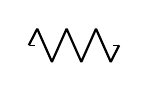
\begin{tikzpicture}[baseline]
                               \draw (0,0) to[R] (1,0);
                           \end{tikzpicture}
                         & 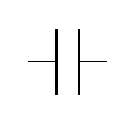
\begin{tikzpicture}[baseline]
                               \draw (0,0) to[C] (1,0);
                           \end{tikzpicture}
                         & 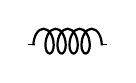
\begin{tikzpicture}[baseline]
                               \draw (0,0) to[L] (1,0);
                           \end{tikzpicture}                                                  \\ \hline
    \end{tblr}
\end{table}

\begin{description}
    \item[Basic elements of a circuit] An RLC circuit has three basic components, shown in the
        table. The general ODE governing an RLC circuit is,
        \begin{align}
            Q                           & = \int I\ \dl t                \\
            LI'' + RI' + \frac{1}{C}\ I & = E'(t)                        \\
            LQ'' + RQ' + \frac{1}{C}\ Q & = E(t) \qquad \text{corollary}
        \end{align}
    \item[Sinusoidally driven RLC] FOr the specific case of a sinusoidal driving EMF,

        \begin{align}
            LI'' + RI' + \frac{1}{C}\ I & = E_{0}\omega \cos(\omega t)        \\
            I_{p}                       & = a\cos(\omega t) + b\sin(\omega t)
        \end{align}


    \item[Reactance] A consolidation of capacitance and inductance derived from the complex
        notation.
        \begin{align}
            I_{p} & = a\cos(\omega t) + b\sin(\omega t)                                          \nonumber \\
            S     & = \omega L - \frac{1}{\omega C}                                                        \\
            I_{p} & = \frac{E_{0}}{R^{2} + S^{2}}\ \Big[-S\cos(\omega t) + R\sin(\omega t)\Big]
        \end{align}

    \item[Impedance] The complex number analog ($ Z $) of ohmic resistance, used to arrive at
        the RLC analog of Ohm's law. It is also known as the apparent resistance \par
        \begin{align}
            |Z|   & = \sqrt{R^{2} + S^{2}}               & E_{0}        & = |Z| I_{0}    \\
            I_{p} & = I_{0} \sin(\omega t - \theta)                                      \\
            I_{0} & = \sqrt{a^{2} + b^{2}}               & \tan(\theta) & = -\frac{a}{b} \\
                  & = \frac{E_{0}}{\sqrt{R^{2} + S^{2}}} &              & = \frac{S}{R}
        \end{align}

    \item[Transient current] Since a real circuit always has $ R > 0 $, the transient
        current always decays exponentially to zero in finite time, with the steady state
        current being the solution of the nh-ODE. \par
\end{description}

The equivalences between mechanical and electrical systems are apparent when looking at
the extreme similarity between the ODEs used to model both systems.

\section{Solution by Variation of Parameters}

The method of undetermined coefficients is restricted to functions $ r(x) $ which are similar
to their derivatives $ r(x)' $. A more general method is introduced here.

\begin{description}
    \item[Variation of Parameters] If $ y_{1}, y_{2} $ form a basis of solutions of the h-ODE,
        and $ W $ is their Wronksian, then the standard form ODE,
        \begin{align}
            y'' + py' + qy & = r                                                                          \\
            y_{h}          & = c_{1}y_{1} + c_{2}y_{2}                                                    \\
            y_{p}          & = -y_{1}\ \int \frac{y_{2}r}{W}\ \dl x + y_{2}\ \int \frac{y_{1}r}{W}\ \dl x
        \end{align}
    \item[Derivation] Starting with a generalization of $ y_{p} $, requires $ p, q, r $ to be
        continuous. \par

        Also, since $ y_{1}, y_{2} $ form a basis of solutions to the h-ODE, their $ W $
        is not zero  anywhere on the interval $ I $ on which they are defined.
        \begin{align}
            y_{p}               & = fy_{1} + gy_{2}                                                                                  \\
            y_{p}'              & = [f'y_{1} + g'y_{2}] + fy_{1}' + gy_{2}'                                                          \\
            f'y_{1} + g'y_{2}   & = 0                                                              &  & \text{artificial constraint} \\
            y_{p}''             & = fy_{1}'' + gy_{2}'' + f'y_{1}' + g'y_{2}'                                                        \\
            f'y_{1}' + g'y_{2}' & = r                                                              &  & \text{substituting into ODE} \\
            f'                  & = \frac{-y_{2}r}{y_{1}y_{2}' - y_{1}'y_{2}} = \frac{-y_{2} r}{W} &  & \text{using}\ W \neq 0       \\
            g'                  & = \frac{y_{1}r}{W}
        \end{align}
        Using the continuity of $ r(x) $, the derivatives $ f', g' $ can be integrated to obtain
        $ f, g $ and complete the derivation.
\end{description}
\chapter{Higher Order Linear ODEs}
\section{Homogeneous Linear ODEs}

\begin{description}
    \item[Linear ODE of nth order] The standard form of an ODE on $ n $-th order is,
        \begin{align}
            y^{(n)} + p_{n-1}(x)y^{(n-1)} + \dots + p_{1}(x)y' + p_{0}(x)y & = r(x)
        \end{align}
        Here, $ \{p_{i}(x)\} $ are any continuous functions of $ x $, and the solution
        $ h(x) $, is defined and $ n $-times differentiable on the interval $ \mathcal{I} $
        in which the set $ \{p_{i}(x)\} $ are defined and continuous.
    \item[Superposition principle] If $ y_{1},\ y_{2} $ are solutions to a linear h-ODE
        of order $ n $, then
        \begin{align}
            c_{1}y_{1} + c_{2}y_{2} = y_{3}
        \end{align}
        is also a solution for some constants $ c_{1}, c_{2} $.
    \item[Linearly Independent functions] A set of functions $ y_{1}(x), \dots, y_{n}(x) $
        are linearly independent (L.I.) on some interval $ \mathcal{I} $ if,
        \begin{align}
            k_{1}y_{1}(x) + \dots + k_{n}y_{n}(x) = 0 \qquad \implies \qquad
            k_{1} = \dots = k_{n} = 0
        \end{align}
        Conversely, if some solution to the above equation exists for which not all $ k_{i} $
        are zero, then the functions are linearly dependent (L.D.)
    \item[Basis of solutions] A set of L.I. solutions to the linear h-ODE of order $ n $.
    \item[General solution] Given a basis of solutions $ \{y_{i}\} $ of the h-ODE,
        \begin{align}
            y & = c_{1}y_{1} + \dots + c_{n}y_{n}
        \end{align}
        is a general solution of the ODE. Particular solutions can be obtained by assigning
        values to the coefficients $ \{c_{i}\} $. \par
        No singular solutions exist which cannot be obtained from the general solution.
    \item[Initial Value Problem] Given the set of $ n $ initial conditions,
        \begin{align}
            y(x_{0}) = K_{0} \quad \ y'(x_{0}) = K_{1}\quad \dots \quad y^{(n)}(X_{0}) = K_{n}
        \end{align}
        There exists a unique solution for a linear h-ODE with coefficients $ \{p_{i}(x)\} $
        continuous on $ \mathcal{I} $ given that $ x_{0} \in \mathcal{I} $.
    \item[Wronskian] Using the determinant of order $ n $,
        \begin{align}
            \renewcommand*{\arraystretch}{1.5}
            W(y_{1},\dots,y_{n}) = \begin{vNiceMatrix}[r, margin]
                                       y_{1}         & y_{2}         & \dots  & y_{n}         \\
                                       y_{1}'        & y_{2}'        & \dots  & y_{n}'        \\
                                       \vdots        & \vdots        & \ddots & \vdots        \\
                                       y_{1}^{(n-1)} & y_{2}^{(n-1)} & \dots  & y_{n}^{(n-1)} \\
                                   \end{vNiceMatrix}
        \end{align}
        If $ W(x) \neq 0 $ for some $ x \in \mathcal{I} $, where the coefficients of the
        h-ODE $ \{p_{i}(x)\} $ are continuous on $ \mathcal{I} $, then the solutions
        $ \{y_{i}(x)\} $ are L.I. \par

        Conversely, if $ W(x) = 0 $ for some $ x = x_{0} \in \mathcal{I} $, then $W \equiv 0$
        identically for all $ x_{0} \in \mathcal{I} $ and the functions are L.D.
    \item[Existence and Uniqueness] If the coefficients $ \{p_{i}(x)\} $ are continuous on
        some interval $ \mathcal{I} $, then the h-ODE has a general solution on $ \mathcal{I} $.
        \par
        Using the fact that the Wronskian is merely the coefficient matrix of the system of linear
        equations in the unknowns $ \{c_{i}\} $ in the general solution, \par
        The Wronskisan of a solution composed of an L.I. basis of solutions is guaranteed to
        cover all possible solutions. Thus the general solution is unique. \par
\end{description}

\section{Homogeneous Linear ODEs with Constant Coefficients}

\begin{description}
    \item[Standard form] In standard form, the h-ODE with constant coefficients of order $ n $,
        alongside its characteristic equation is,
        \begin{align}
            y^{(n)} + a_{n-1}y^{(n-1)} + \dots + a_{1}y' + a_{0} & = 0             \\
            y_{h}                                                & = e^{\lambda x} \\
            \lambda^{n} + a_{n-1}\lambda^{n-1} + \dots a_{1}\lambda + a_{0} = 0
        \end{align}
    \item[Distinct real roots] Each distinct root $ \lambda_{k} $ corresponds to a solution
        to the ODE $ e^{k\lambda} $
        \begin{align}
            W & = \begin{vNiceMatrix}[r, margin]
                      e^{\lambda_{1}x}                  & e^{\lambda_{2}x}                  & \dots  & e^{\lambda_{n}x}                  \\
                      \lambda_{1}e^{\lambda_{1}x}       & \lambda_{2}e^{\lambda_{2}x}       & \dots  & \lambda_{n}e^{\lambda_{n}x}       \\
                      \lambda_{1}^{2}e^{\lambda_{1}x}   & \lambda_{2}^{2}e^{\lambda_{2}x}   & \dots  & \lambda_{n}^{2}e^{\lambda_{n}x}   \\
                      \vdots                            & \vdots                            & \ddots & \vdots                            \\
                      \lambda_{1}^{n-1}e^{\lambda_{1}x} & \lambda_{2}^{n-1}e^{\lambda_{2}x} & \dots  & \lambda_{n}^{n-1}e^{\lambda_{n}x}
                  \end{vNiceMatrix}
        \end{align}
    \item[Vandermode determinant] A simplified version of the above determinant given by,
        \begin{align}
            W & = \exp\left( x\sum_{k=1}^{n} \lambda_{k} \right)\ \begin{vNiceMatrix}[r, margin]
                                                                      1                 & 1                 & \dots  & 1                 \\
                                                                      \lambda_{1}       & \lambda_{2}       & \dots  & \lambda_{n}       \\
                                                                      \lambda_{1}^{2}   & \lambda_{2}^{2}   & \dots  & \lambda_{n}^{2}   \\
                                                                      \vdots            & \vdots            & \ddots & \vdots            \\
                                                                      \lambda_{1}^{n-1} & \lambda_{2}^{n-1} & \dots  & \lambda_{n}^{n-1}
                                                                  \end{vNiceMatrix}                       \\
              & = \exp\left( x\sum_{k=1}^{n} \lambda_{k} \right)\ (-1)^{n(n-1)/2} \cdot \prod_{j = 1}^{n}\ (\lambda_{j} - \lambda_{k}) \qquad n \geq j > k
        \end{align}
        The above expression is simply the difference between all possible combinations of roots.
        Since the first term is a product of exponentials, it is never zero. \par
        So, the Wronksian provides L.I only if all the roots are distinct, and thus none
        of the terms $ (\lambda_{j} - \lambda_{k}) $ are zero.
    \item[Repeated roots] For repeated roots of multiplicity $ m $, whether real or complex,
        \begin{align}
            y_{1}  & = e^{\lambda x}      & z_{1}, z_{2}     & = e^{\alpha x}\sin \beta x, e^{\alpha x} \cos \beta x           \\
            y_{2}  & = xe^{\lambda x}     & z_{3}, z_{4}     & = xe^{\alpha x}\sin \beta x, xe^{\alpha x} \cos \beta x         \\
            y_{3}  & = x^{2}e^{\lambda x} & z_{5}, z_{6}     & = x^{2}e^{\alpha x}\sin \beta x, x^{2}e^{\alpha x} \cos \beta x \\
            \vdots &                      & \vdots           & \nonumber                                                       \\
            y_{m}  & = x^{m}e^{\lambda x} & z_{2m-1}, z_{2m} & = x^{m}e^{\alpha x}\sin \beta x, x^{m}e^{\alpha x} \cos \beta x
        \end{align}
        Other solutions are obtained by multiplying higher powers of $ x $ to existing solutions.
        \par
        To derive the above multiple roots factor, consider the root $ \lambda_{1} $ with
        multiplicity $ m $,
        \begin{align}
            \mathcal{L}[y]             & = y^{(n)} + a_{n-1}y^{(n-1)} + \dots + a_{1}y' + a_{0}y                              \\
            \mathcal{L}[e^{\lambda x}] & = (\lambda^{n} + a_{n-1}\lambda^{n-1} + \dots + a_{1}\lambda + a_{0})\ e^{\lambda x} \\
                                       & = (\lambda - \lambda_{1})^{m} \cdot h(\lambda) \cdot e^{\lambda x}
        \end{align}
        Here $ h(\lambda) $ is the leftover polynomial after factoring out all the $ \lambda_{1} $.
        \begin{align}
            \diffp**{\lambda}{\mathcal{L}[e^{\lambda x}]}
             & = \mathcal{L}\left[ \diffp**{\lambda}{e^{\lambda x}} \right]
            = \mathcal{L}[xe^{\lambda x}]                                                       \\
             & = m(\lambda - \lambda_{1})^{m-1} \cdot h(\lambda)e^{\lambda x} \nonumber         \\
             & + (\lambda - \lambda_{1})^{m} \cdot \diffp**{\lambda}{[h(\lambda)e^{\lambda x}]} \\
        \end{align}
        Since $ m > 2 $, the RHS is zero at $ \Lambda = \lambda_{1} $. This means that
        $\mathcal{L}[xe^{\lambda x}] = 0$, and thus $ xe^{\lambda x} $ is a solution.
        \par Further differentiation w.r.t. $ \lambda $ can be used to arrive at further
        solutions corresponding to $ \lambda_{1} $.
\end{description}

\section{Nonhomogeneous Linear ODEs}

\begin{description}
    \item[Standard form] Ensuring the coefficient of $ y^{(n)} $ is $ 1 $,
        \begin{align}
            y^{(n)} + a_{n-1}y^{(n-1)} + \dots + a_{1}y' + a_{0} & = r(x)                \\
            y                                                    & = y_{h}(x) + y_{p}(x)
        \end{align}
        The Initial value problem is the same as for h-ODEs.
    \item[Undetermined coefficients] Similar to second order nh-ODEs, higher order ODEs
        can be solved using the pre-factor $ x^{m} $ to deal with roots of multiplicity $ m $.
    \item[Variation of parameters] Generalizing to order $ n $,
        \begin{align}
            y_{p} & = \sum_{k = 1}^{n}\ y_{k} \int \frac{W_{k}}{W}\ r \dl x
        \end{align}
        $ W $ is the Wronskian of the h-ODE with a basis of solutions $ \{y_{1}, y_{2},
            \dots,y_{n}\} $. $ W_{k} $ is the reduced Wronskian produced by replacing the
        $ k $-th column of $ W $ with the column vector $ [0\ 0\ \dots\ 0\ 1]^{T} $
\end{description}
\chapter{Systems of ODEs, Phase Plane, Qualitative Methods}
\section{Systems of ODEs as Models in Engineering Applications}
\begin{description}
    \item[Conversion to system of ODEs] Any ODE of order $ n $ can be converted to a system
        of $ n $ ODEs of first order. Linear algebra provides easy methods of solving this
        system of linear equations using eigenvectors and eigenvalues.
        \begin{align}
            y^{(n)}                          & = F\left( t,\ y,\ y',\ y'',\ \dots,\ y^{(n-1)} \right)  \\
            \text{Set} \qquad y_1            & = y, \qquad y_2 = y', \quad \dots \quad y_n = y^{(n-1)} \\
            \text{System becomes}\qquad y_1' & = y_2 \nonumber                                         \\
            y_2'                             & = y_3 \nonumber                                         \\
            \vdots \nonumber                                                                           \\
            y_{n-1}'                         & = y_n \nonumber                                         \\
            y_n'                             & = F(t,\ y_1,\ y_2,\ \dots,\ y_n)
        \end{align}
    \item[Eigenvalues] When a system of linear equations is expressed in vector form,
        \begin{align}
            \renewcommand*{\arraystretch}{1.5}
            y_1'                 & = a_{11}y_1 + a_{12}y_2 \nonumber         \\
            y_2'                 & = a_{21}y_1 + a_{22}y_2                   \\
            \bmatcol{y_1'}{y_2'} & = \bmattt{a_{11}}{a_{12}}{a_{21}}{a_{22}} \\
            \vec{y'}             & = \vec{A}\vec{y}
        \end{align}
        For a matrix equation to have a non-trivial solution,
        \begin{align}
            \vec{A}\vec{x}                     & = \lambda \vec{x}                         \\
            (\vec{A} - \lambda\vec{I}) \vec{x} & = 0                                       \\
            \det(\vec{A} - \lambda\vec{I})     & = \begin{vNiceMatrix}[r, margin]
                                                       (a_{11} - \lambda) & a_{12}             \\
                                                       a_{21}             & (a_{22} - \lambda)
                                                   \end{vNiceMatrix}
        \end{align}
        This quadratic equation has solutions $ \lambda_1, \lambda_2 $ called eigenvalues.
        The corresponding eigenvectors $ \vec{v^{(1)}}, \vec{v^{(2)}} $ are found as
        solutions of the respective systems.
        \begin{align}
            (\vec{A} - \lambda_1\vec{I}) \vec{v^{(1)}} & = 0 \\
            (\vec{A} - \lambda_2\vec{I}) \vec{v^{(2)}} & = 0
        \end{align}
\end{description}

\section{Basic Theory of Systems of ODEs, Wronskian}
\begin{description}
    \item[General system of ODEs] Using a set of functions $ \{f_i\} $,
        \begin{align}
            y_1'     & = f_1(t,\ y_1,\ \dots,\ y_n) \\
            y_2'     & = f_2(t,\ y_1,\ \dots,\ y_n) \\
            \vdots                                  \\
            y_n'     & = f_n(t,\ y_1,\ \dots,\ y_n) \\
            \text{converting to vector notation,}   \\
            \vec{y'} & = \vec{f}(t, \vec{y})
        \end{align}
        Introducing the set of solutions as a vector, and another vector for the I.C.
        \begin{align}
            \vec{y}      & = \vec{h}(t) = \begin{bNiceMatrix}[r, margin]
                                              h_1(t) \\ h_2(t) \\ \vdots \\ h_n(t)
                                          \end{bNiceMatrix} &
            \vec{y}(t_0) & = \vec{K} = \begin{bNiceMatrix}[r, margin]
                                           K(0) \\ K(1) \\ \vdots \\ K_n
                                       \end{bNiceMatrix}
        \end{align}
    \item[Existence and Uniqueness] Given the preconditions,
        \begin{align}
            \{f_1,\ f_2,\ \dots,\ f_n\} \qquad       &
            \text{are continuous}                      \\
            \left\{ \diffp{f_i}{y_k} \right\} \qquad &
            \text{are continuous for all}\ j,k
        \end{align}
        Continuity is guaranteed in some point $ (t_0,\ K_0,\ K_1,\ \dots,\ K_n) $ in
        this interval of continuity in $ (t,\ y_0,\ y_1,\ \dots,\ y_n) $ space. \par
        Then, a solution to the system of ODEs exists in some interval
        $ t \in (t_0 - \alpha, t_0 + \alpha) $ and is guaranteed to be unique.
    \item[Linear System] A subset of the above general system of ODEs obeying,
        \begin{align}
            \begin{bNiceMatrix}[r, margin]
                y_1' \\ \vdots \\ y_n'
            \end{bNiceMatrix} & = \begin{bNiceMatrix}[r, margin]
                                      a_{11} & \dots  & a_{1n} \\
                                      \vdots & \ddots & \vdots \\
                                      a_{n1} & \dots  & a_{nn}
                                  \end{bNiceMatrix} \begin{bNiceMatrix}[r, margin]
                                                        y_1 \\ \vdots \\ y_n
                                                    \end{bNiceMatrix} + \begin{bNiceMatrix}[r, margin]
                                                                            g_1 \\ \vdots \\ g_n
                                                                        \end{bNiceMatrix} \\
            \vec{y'}                       & = \vec{Ay} + \vec{g}
        \end{align}
        The above system is homogeneous if $ \vec{g} = 0 $, with $ a_{jk} =
            \difsp{f_j}{y_k} $. \par
        If the elements of $ \vec{g} $ and $ \vec{a} $ are continuous functions of
        $ t $ in some interval $ t \in (\alpha, \beta) $ which contains the point
        $ t = t_0 $, then a solution exists and is guaranteed to be unique.
    \item[Superposition Principle] If $ \vec{y^{(1)}} $ and $ \vec{y^{(2)}} $ are
        solutions of the h-linear system of ODEs on some interval, then
        \begin{align}
            \vec{y^{(3)}} & = c_1 \vec{y^{(1)}} + c_2 \vec{y^{(2)}}
        \end{align}
        is also a solution. (using the linearity of matrix multiplication and of
        differentiation)
    \item[Basis] A set of L.I. solutions $ \{ \vec{y^{(i)}} \} $ form a basis in the
        interval $ \mathcal{J} $ if the elements of $ \vec{a} $ are continuous in
        $ \mathcal{J} $. \par

        A linear combination of this basis is a general solution that contains all
        possible solutions.
    \item[Wronskian] The old Wronskian of a set of solutions $ \{z_i\} $ becomes
        a matrix whose columns are members of the basis set $ \vec{y^{(i)}} $. \par

        The rows are successive derivatives (transformed into subscript variables).
        \begin{align}
            \begin{bNiceMatrix}[r, margin]
                z_1         & z_1         & \dots  & z_n         \\
                z_1'        & z_2'        & \dots  & z_n'        \\
                \vdots      & \vdots      & \ddots & \vdots      \\
                z_1^{(n-1)} & z_2^{(n-1)} & \dots  & z_n^{(n-1)}
            \end{bNiceMatrix} & \to
            \begin{bNiceMatrix}[r, margin]
                y_1^{(1)} & y_1^{(2)} & \dots  & y_1^{(n)} \\
                y_2^{(1)} & y_2^{(2)} & \dots  & y_2^{(n)} \\
                \vdots    & \vdots    & \ddots & \vdots    \\
                y_n^{(1)} & y_n^{(2)} & \dots  & y_n^{(n)}
            \end{bNiceMatrix}                                                \\
            W = \det(\vec{Y})                                   &
            = \det\begin{bNiceMatrix}[r, margin] \vec{y^{(1)}} &
                   \dots                     & \vec{y^{(n)}}\end{bNiceMatrix} \\
        \end{align}
        The Wronskian is either identically zero everywhere (if L.D.) or nowhere
        (if L.I.) in the interval $ \mathcal{J} $ under consideration.

    \item[Fundamental matrix] The above matrix $ \vec{Y} $ is called a fundamental
        matrix if the solutions $ \{\vec{y^{(i)}}\} $ form a basis.
        \begin{align}
            \vec{y}                        & = c_1\vec{y^{(1)}} + \dots + c_2\vec{y^{(n)}}                            \\
            \vec{y}                        & = \vec{Yc}                                                               \\
            \begin{bNiceMatrix}[r, margin]
                y_1 \\ \vdots \\ y_n
            \end{bNiceMatrix} & = \begin{bNiceMatrix}[r, margin] \vec{y^{(1)}} &
                                             & \vec{y^{(n)}}\end{bNiceMatrix}
            \begin{bNiceMatrix}[r, margin]
                c_1 \\ \vdots \\ c_n
            \end{bNiceMatrix}
        \end{align}
\end{description}

\section{Constant-Coefficient Systems, Phase Plane Method}
\begin{description}
    \item[Constant coefficient system] If the matrix $ \vec{a} $ has terms
        independent of $ t $, then the initial guess
        \begin{align}
            \vec{y'} & = \vec{Ay}        & \vec{y} & = \vec{x} e^{\lambda t} \\
            \vec{Ax} & = \lambda \vec{x}
        \end{align}
        leads to an eigenvalue problem. Here, $ \lambda, \vec{x} $ are the pairs
        of eigenvalues and eigenvectors respectively.
    \item[L.I. eigenvectors condition] For the above matrix $ \vec{A} $ to have
        a set of L.I. eigenvectors (as is common in real world applications), conditions
        are one of
        \begin{itemize}
            \item $\vec{A}$ is symmetric. $ a_{jk} = a_{kj} $ or $\vec{A} = \vec{A^T} $.
            \item $\vec{A}$ is skew symmetric. $ a_{jk} = -a_{kj} $
                  or $\vec{A} = -\vec{A^T} $.
            \item $ \vec{A} $ has $ n $ distinct eigenvalues.
        \end{itemize}
    \item[General solution] If $ \vec{A} $ has a set of L.I. eigenvectors as above,
        then the corresponding solutions form a basis. \par
        A general solution is of the form,
        \begin{align}
            \vec{y} & = c_1 \vec{x^{(1)}}e^{\lambda_1 t} + \quad \cdots \quad
            + c_n \vec{x^{(n)}}e^{\lambda_n t}
        \end{align}
        From this point onwards, the limited case of two member families of
        ODEs is taken up.
\end{description}


\begin{description}
    \item[Phase plane] The use of a parameter to plot the two solutions $ y_1 $ vs.
        $y_2$ instead of the usual pair of $ y $ vs. $ t $ curves.
    \item[Critical Points] Points in the phase plane where the tangent direction is
        not defined (for example at $ (0, 0) $ in the expression below).
        \begin{align}
            \diff{y_2}{y_1} & = \frac{y_2' \dl t}{y_1' \dl t} = \frac{y_2'}{y_1'}   \\
                            & = \frac{a_{21}y_1 + a_{22}y_2}{a_{11}y_1 + a_{12}y_2}
        \end{align}
    \item[Improper Node] A critical point $ P_0 $ at which all but two trajectories
        have the same limiting direction of the tangent $ L_1 $. The two exceptional
        trajectories also have a different (and equal) limit $ L_2 $.

    \item[Proper Node] A critical point at which every trajectory has a distinct
        limiting direction, and for any given direction $ \vec{d} $, there is some
        trajectory whose limiting direction at $ P_0 $ is equal to $ \vec{d} $.
    \item[Saddle Point] Two incoming and two outgoing trajectories intersect $ P_0 $,
        while all other trajectories bypass $ P_0 $.
    \item[Center] A critical point, enclosed by many closed trajectories, none of
        which ever pass through $ P_0 $.
    \item[Spiral] A critical point which all trajectories approach as
        $ t \to \infty $ which otherwise resembles a center.
    \item[Degenerate Node] In the (almost never physical) case when no basis of
        eigenvectors can be found. The usual condition is that $ \vec{A} $ is neither
        symmetric nor skew-symmetric and happens to have degenerate eigenvalues.
        \begin{figure}[H]
            \centering
            \begin{subfigure}[b]{0.49\textwidth}
                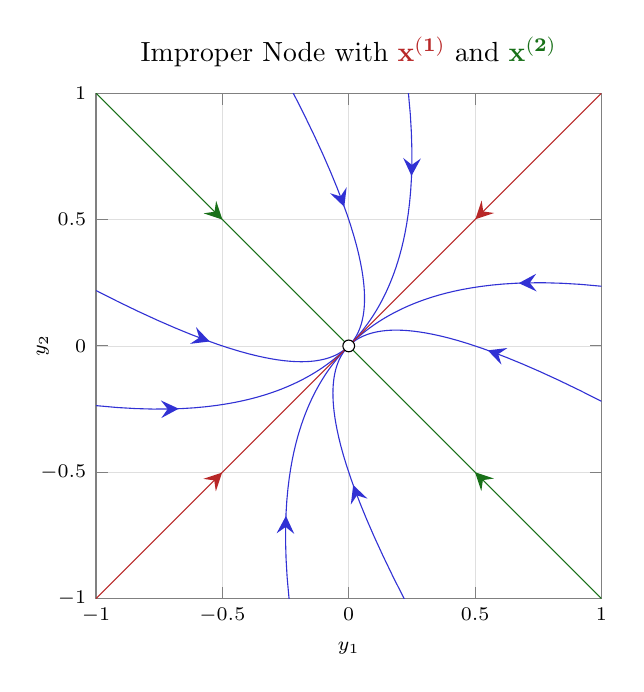
\begin{tikzpicture}
                    \begin{axis}[
                            declare function = {
                                    u(\x) = e^(-2*\x);
                                    v(\x) = e^(-4*\x);
                                },
                            xmin = -1, xmax = 1, ymin = -1, ymax = 1,
                            % restrict y to domain = -1:1,
                            title = {Improper Node with
                                    ${\color{y_p} \vec{x^{(1)}}}$ and
                                    ${\color{y_h} \vec{x^{(2)}}}$},
                            xlabel = $ y_1 $,
                            ylabel = $ y_2 $, ylabel shift = {-1em},
                            axis equal,
                            width = 8cm,
                            legend pos = north west,
                            grid = both,
                            domain = 0:3,
                            Ani]
                        \foreach \c in {-0.5, -1, 0.5, 1} {%
                                \edef\temp{%
                                    \noexpand \addplot[ samples = 100, color=blue3,
                                        arrow inside={end=stealth,opt={scale=2}}{0.65}]
                                    ({\c*u(x) + v(x)}, {\c*u(x) - v(x)});
                                    \noexpand \addplot[ samples = 100, color=blue3,
                                        arrow inside={end=stealth,opt={scale=2}}{0.65}]
                                    ({\c*u(x) - v(x)}, {\c*u(x) + v(x)});
                                }\temp
                            }
                        \addplot[ samples = 100, color=y_p,
                            arrow inside={end=stealth,opt={scale=2}}{0.5}]
                        ({u(x)}, {u(x)});
                        \addplot[ samples = 100, color=y_h,
                            arrow inside={end=stealth,opt={scale=2}}{0.5}]
                        ({v(x)}, {-v(x)});
                        \addplot[ samples = 100, color=y_p,
                            arrow inside={end=stealth,opt={scale=2}}{0.5}]
                        ({-u(x)}, {-u(x)});
                        \addplot[ samples = 100, color=y_h,
                            arrow inside={end=stealth,opt={scale=2}}{0.5}]
                        ({-v(x)}, {v(x)});
                        \node[GraphNode, fill = white, draw = black] at (axis cs:0,0) {};
                    \end{axis}
                \end{tikzpicture}
            \end{subfigure}
            \hfill
            \begin{subfigure}[b]{0.49\textwidth}
                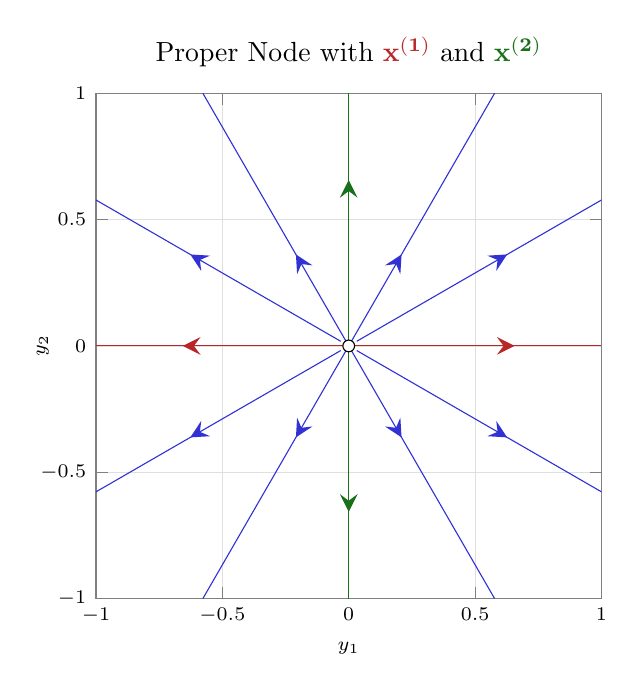
\begin{tikzpicture}
                    \begin{axis}[
                            declare function = {
                                    u(\x) = e^(\x);
                                    v(\x) = e^(\x);
                                },
                            xmin = -1, xmax = 1, ymin = -1, ymax = 1,
                            % restrict y to domain = -1:1,
                            title = {Proper Node with
                                    ${\color{y_p} \vec{x^{(1)}}}$ and
                                    ${\color{y_h} \vec{x^{(2)}}}$},
                            xlabel = $ y_1 $,
                            ylabel = $ y_2 $, ylabel shift = {-1em},
                            axis equal,
                            width = 8cm,
                            legend pos = north west,
                            grid = both,
                            domain = -4:0,
                            Ani]
                        \foreach \c in {-sqrt(3), -1/sqrt(3), sqrt(3), 1/sqrt(3)} {%
                                \edef\temp{%
                                    \noexpand \addplot[ samples = 100, color=blue3,
                                        arrow inside={end=stealth,opt={scale=2}}{0.35}]
                                    ({\c*u(x)}, {-v(x)});
                                    \noexpand \addplot[ samples = 100, color=blue3,
                                        arrow inside={end=stealth,opt={scale=2}}{0.35}]
                                    ({\c*u(x)}, {v(x)});
                                }\temp
                            }
                        \addplot[ samples = 100, color=y_p,
                            arrow inside={end=stealth,opt={scale=2}}{0.65}]
                        ({u(x)}, {0});
                        \addplot[ samples = 100, color=y_h,
                            arrow inside={end=stealth,opt={scale=2}}{0.65}]
                        ({0}, {-v(x)});
                        \addplot[ samples = 100, color=y_p,
                            arrow inside={end=stealth,opt={scale=2}}{0.65}]
                        ({-u(x)}, {0});
                        \addplot[ samples = 100, color=y_h,
                            arrow inside={end=stealth,opt={scale=2}}{0.65}]
                        ({0}, {v(x)});
                        \node[GraphNode, fill = white, draw = black] at (axis cs:0,0) {};
                    \end{axis}
                \end{tikzpicture}
            \end{subfigure}
        \end{figure}

        \begin{figure}[H]
            \centering
            \begin{subfigure}[b]{0.48\textwidth}
                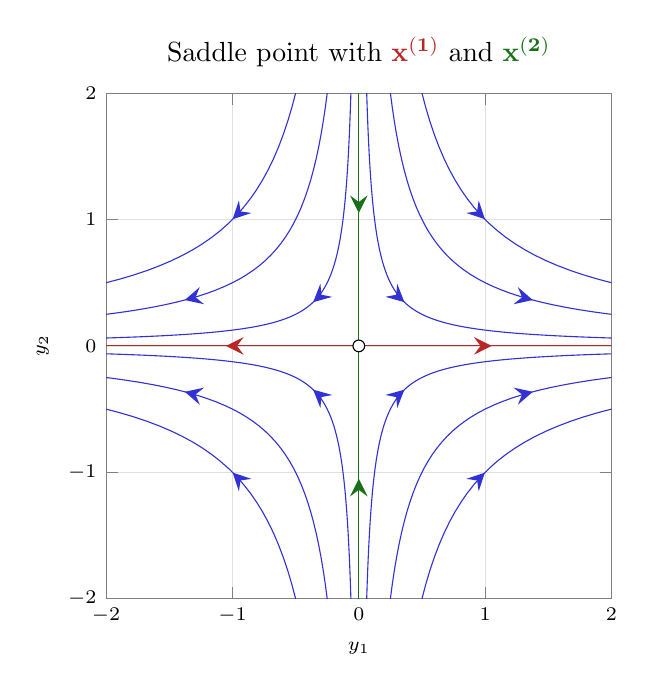
\begin{tikzpicture}
                    \begin{axis}[
                            declare function = {
                                    u(\x) = e^(\x);
                                    v(\x) = e^(-\x);
                                },
                            xmin = -2, xmax = 2, ymin = -2, ymax = 2,
                            % restrict y to domain = -1:1,
                            title = {Saddle point with
                                    ${\color{y_p} \vec{x^{(1)}}}$ and
                                    ${\color{y_h} \vec{x^{(2)}}}$},
                            xlabel = $ y_1 $,
                            ylabel = $ y_2 $,
                            axis equal,
                            width = 8cm,
                            legend pos = north west,
                            grid = both,
                            domain = -3:3,
                            Ani]
                        \foreach \c in {1/8, 1/2, 1} {%
                                \edef\temp{%
                                    \noexpand \addplot[ samples = 100, color=blue3,
                                        arrow inside={end=stealth,opt={scale=2}}{0.5, 0.7, 0.8, 0.9}]
                                    ({\c*u(x)}, {-v(x)});
                                    \noexpand \addplot[ samples = 100, color=blue3,
                                        arrow inside={end=stealth,opt={scale=2}}{0.5, 0.7, 0.8, 0.9}]
                                    ({\c*u(x)}, {v(x)});
                                    \noexpand \addplot[ samples = 100, color=blue3,
                                        arrow inside={end=stealth,opt={scale=2}}{0.5, 0.7, 0.8, 0.9}]
                                    ({-\c*u(x)}, {-v(x)});
                                    \noexpand \addplot[ samples = 100, color=blue3,
                                        arrow inside={end=stealth,opt={scale=2}}{0.5, 0.7, 0.8, 0.9}]
                                    ({-\c*u(x)}, {v(x)});
                                }\temp
                            }
                        \addplot[ samples = 100, color=y_p,
                            arrow inside={end=stealth,opt={scale=2}}{0.05}]
                        ({u(x)}, {0});
                        \addplot[ samples = 100, color=y_h,
                            arrow inside={end=stealth,opt={scale=2}}{0.95}]
                        ({0}, {-v(x)});
                        \addplot[ samples = 100, color=y_p,
                            arrow inside={end=stealth,opt={scale=2}}{0.05}]
                        ({-u(x)}, {0});
                        \addplot[ samples = 100, color=y_h,
                            arrow inside={end=stealth,opt={scale=2}}{0.95}]
                        ({0}, {v(x)});
                        \node[GraphNode, fill = white, draw = black] at (axis cs:0,0) {};
                    \end{axis}
                \end{tikzpicture}
            \end{subfigure}
            \hfill
            \begin{subfigure}[b]{0.48\textwidth}
                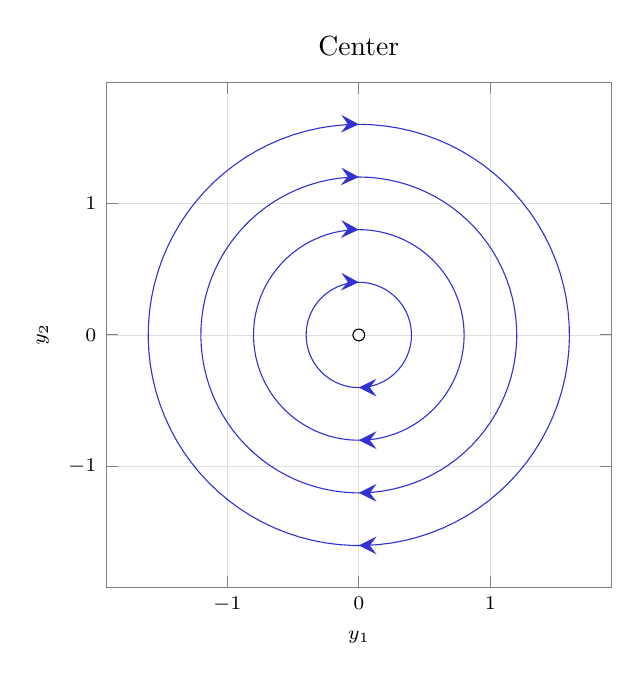
\begin{tikzpicture}
                    \begin{axis}[
                            % xmin = -1, xmax = 1, ymin = -1, ymax = 1,
                            % restrict y to domain = -1:1,
                            title = {Center},
                            xlabel = $ y_1 $,
                            ylabel = $ y_2 $,
                            axis equal,
                            width = 8cm,
                            legend pos = north west,
                            grid = both,
                            domain = 0:2*pi,
                            Ani]
                        \foreach \c in {0.4,0.8,...,2.0} {%
                                \edef\temp{%
                                    \noexpand \addplot[ samples = 100, color=blue3,
                                        arrow inside={end=stealth,opt={scale=2}}{0, 0.5}]
                                    ({\c*sin(x)}, {\c*cos(x)});
                                }\temp
                            }
                        \node[GraphNode, fill = white, draw = black] at (axis cs:0,0) {};
                    \end{axis}
                \end{tikzpicture}
            \end{subfigure}
        \end{figure}

        \begin{figure}[H]
            \centering
            \begin{subfigure}[b]{0.49\textwidth}
                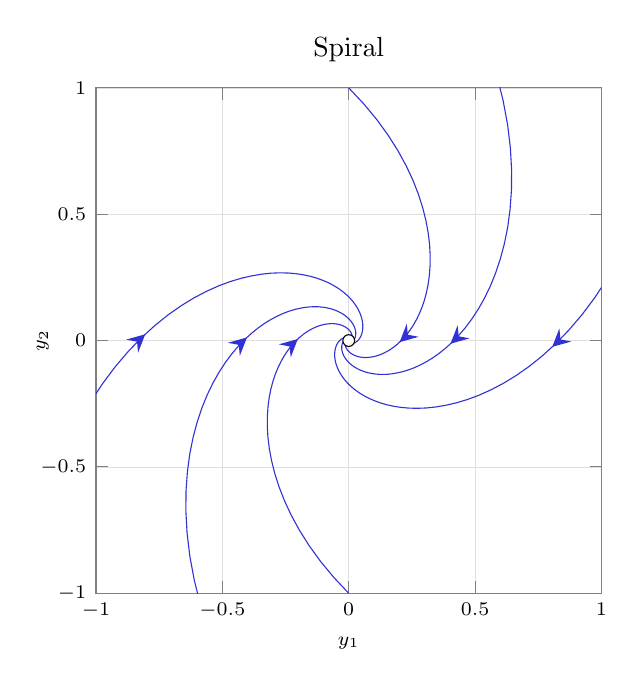
\begin{tikzpicture}
                    \begin{axis}[
                            xmin = -1, xmax = 1, ymin = -1, ymax = 1,
                            % restrict y to domain = -1:1,
                            title = {Spiral},
                            xlabel = $ y_1 $,
                            ylabel = $ y_2 $, ylabel shift = {-1em},
                            axis equal,
                            width = 8cm,
                            legend pos = north west,
                            grid = both,
                            domain = 0:2*pi,
                            Ani]
                        \foreach \c in {1,2,4} {%
                                \edef\temp{%
                                    \noexpand \addplot[ samples = 100, color=blue3,
                                        arrow inside={end=stealth,opt={scale=2}}{0.8}]
                                    ({\c*e^(-x)*sin(x)}, {\c*e^(-x)*cos(x)});
                                    \noexpand \addplot[ samples = 100, color=blue3,
                                        arrow inside={end=stealth,opt={scale=2}}{0.8}]
                                    ({-\c*e^(-x)*sin(x)}, {-\c*e^(-x)*cos(x)});
                                }\temp
                            }
                        \node[GraphNode, fill = white, draw = black] at (axis cs:0,0) {};
                    \end{axis}
                \end{tikzpicture}
            \end{subfigure}
            \hfill
            \begin{subfigure}[b]{0.49\textwidth}
                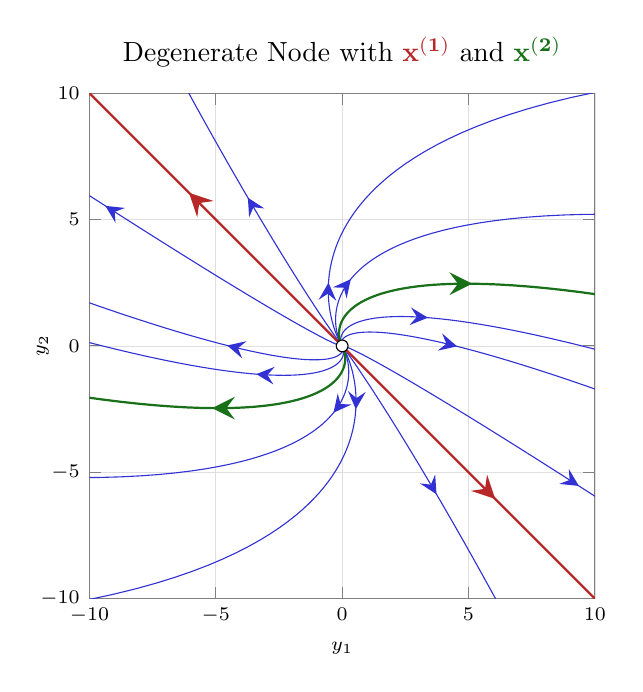
\begin{tikzpicture}
                    \begin{axis}[
                            xmin = -10, xmax = 10, ymin = -10, ymax = 10,
                            % restrict y to domain = -1:1,
                            title = {Degenerate Node with
                                    ${\color{y_p} \vec{x^{(1)}}}$ and
                                    ${\color{y_h} \vec{x^{(2)}}}$},
                            xlabel = $ y_1 $,
                            ylabel = $ y_2 $, ylabel shift = {-1em},
                            axis equal,
                            width = 8cm,
                            legend pos = north west,
                            grid = both,
                            domain = -1:1,
                            Ani]
                        \foreach \c in {1/2,1/4,2} {%
                                \edef\temp{%
                                    \noexpand \addplot[thin, samples = 100, color=blue3,
                                        arrow inside={end=stealth,opt={scale=2}}{0.15}]
                                    ({(\c + x)*e^(3*x)}, {(-\c - x + 1)*e^(3*x)});
                                    \noexpand \addplot[thin, samples = 100, color=blue3,
                                        arrow inside={end=stealth,opt={scale=2}}{0.15}]
                                    ({(\c - x)*e^(3*x)}, {(-\c + x - 1)*e^(3*x)});
                                    \noexpand \addplot[thin, samples = 100, color=blue3,
                                        arrow inside={end=stealth,opt={scale=2}}{0.15}]
                                    ({(-\c + x)*e^(3*x)}, {(\c - x + 1)*e^(3*x)});
                                    \noexpand \addplot[thin, samples = 100, color=blue3,
                                        arrow inside={end=stealth,opt={scale=2}}{0.15}]
                                    ({(-\c - x)*e^(3*x)}, {(\c + x - 1)*e^(3*x)});
                                }\temp
                            }
                        \addplot[thick, samples = 100, color=y_p,
                            arrow inside={end=stealth,opt={scale=2}}{0.3}]
                        ({e^(3*x)}, {-e^(3*x)});
                        \addplot[thick, samples = 100, color=y_p,
                        arrow inside={end=stealth,opt={scale=2}}{0.3}]
                        (-{e^(3*x)}, {e^(3*x)});
                        \addplot[thick, samples = 100, color=y_h,
                            arrow inside={end=stealth,opt={scale=2}}{0.3}]
                        ({x*e^(3*x)}, {(-x+1)*e^(3*x)});
                        \addplot[thick, samples = 100, color=y_h,
                            arrow inside={end=stealth,opt={scale=2}}{0.3}]
                        ({-x*e^(3*x)}, {-1*(-x+1)*e^(3*x)});
                        \node[GraphNode, fill = white, draw = black] at (axis cs:0,0) {};
                    \end{axis}
                \end{tikzpicture}
            \end{subfigure}
        \end{figure}
\end{description}

\section{Criteria for Critical Points, Stability}
\begin{description}
    \item[Characteristic equation] For the two member system of linear ODEs with
        constant coefficients,
        \begin{align}
            \vec{A}                        & = \bmattt{a_{11}}{a_{12}}{a_{21}}{a_{22}} \\
            \det(\vec{A} - \lambda\vec{I}) & =
            \lambda^{2} - (a_{11} + a_{22})\lambda + \det(\vec{A}) = 0                 \\
            \lambda^{2} - p\lambda + q     & = 0
        \end{align}
    \item[Critical point categories] Rearranging the characteristic equation into its
        factors $ \lambda_1,\ \lambda_2 $,
        \begin{align}
            p                           & = \lambda_1 + \lambda_2       &
            q                           & = \lambda_1 \lambda_2           \\
            \text{Discriminant}\ \Delta & = p^{2} - 4q                  &
            \Delta                      & = (\lambda_1 - \lambda_2)^{2}
        \end{align}
        \begin{table}[ht]
            \centering
            \SetTblrInner{rowsep=0.5em}
            \begin{tblr}{colspec={Q[r]|Q[l]}, colsep = 2em}
                \textbf{Critical Point} &
                \textbf{Eigenvalues} $ \lambda_1, \lambda_2 $            \\ \hline[dotted]
                Node                    & Real, same sign                \\
                Saddle point            & Real, opposite signs           \\
                Center                  & Purely imaginary               \\
                Spiral point            & Complex with nonzero real part \\ \hline
            \end{tblr}
        \end{table}
    \item[Stability] From physics, stability is a measure of the effect in the future
        of a small change in the system at present time.
    \item[Stable critical point] If for every disk $ D_\epsilon $ centered on $ P_0 $,
        there is a disk $ D_{\delta} $ with $ \delta, \epsilon >0 $, such that every trajectory
        which has $ P(t = t_1) = P_1 \in D_{\delta}$ has all its points corresponding to
        $ t \geq t_1 $ in $ D_{\epsilon} $.
    \item[Attractive critical point] Every trajectory in $ D_\delta $ for a stable
        critical point, approaches $ P_0 $ asymptotically as $ t \to \infty $.

        \begin{table}[ht]
            \centering
            \SetTblrInner{rowsep=0.5em}
            \begin{tblr}{colspec={Q[r]|Q[l]}, colsep = 2em}
                \textbf{Stability}    &
                \textbf{Condition on} $ \vec{p},\ \vec{q} $        \\ \hline[dotted]
                Stable and attractive & $ p<0 $ and $ q > 0 $      \\
                Stable                & $ p \leq 0 $ and $ q > 0 $ \\
                Unstable              & $ p > 0 $ or $\ \ q < 0 $  \\ \hline
            \end{tblr}
        \end{table}
\end{description}

\section{Qualitative Methods for Nonlinear Systems}
\begin{description}
    \item[Assumptions] The system of ODEs is autonomous, and the functions $ f_1, f_2 $
        are independent of $ t $. \par
        Also, the system of ODEs has finitely many critical points. This
        means that each critical point is isolated. \par
        For analysis, each critical point is treated as the origin when being analyzed,
        using the coordinate transformation,
        \begin{align}
            P_0         & = (a, b)  & (a, b)      & \to (0, 0) \\
            \tilde{y_i} & = y_1 - a & \tilde{y_2} & = y_2 - b
        \end{align}
    \item[Linearization] The system is linearlised around its critical point
        $ (0, 0) $ using,
        \begin{align}
            \vec{y} & = \vec{f}(\vec{y}) \equiv \vec{Ay} + \vec{h}(\vec{y}) \\
            y_1'    & = a_{11}y_1 + a_{12}y_2 + h_1(y_1, y_2)               \\
            y_2'    & = a_{21}y_1 + a_{22}y_2 + h_2(y_1, y_2)
        \end{align}
        Notice $ \vec{A} $ here is independent of $ y $ since $ P_0  = (0, 0)$ is
        a critical point giving. \par
        If $ f_1, f_2 $ are continuous and have continuous partial derivatives in a
        region around $ P_0 $, and if $ \det(\vec{A}) \neq 0 $, then the kind and
        stability of the critical points of the original system are the same as
        those of the linearized system. \par
        Exceptions occur if the linearized system has equal roots or purely imaginary
        roots.
        The general method is as follows,
        \begin{enumerate}
            \item Set up the mathematical model.
            \item Identify the critical points as conditions for $ \vec{y} = 0 $
            \item Drop all nonlinear terms in order to linearize the system
            \item Treat each critical point in turn, transforming coordinates as
                  needed.
        \end{enumerate}
    \item[Transformation to first order ODE] A second order autonomous ODE can
        be transformed using,
        \begin{align}
            F(y, y', y'') & = 0                    & y & = y_1, \qquad y' = y_2 \\
            y''           & = \diff{y_2}{y_1}\ y_2
        \end{align}
    \item[Limit Cycle] A closed trajectory in phase space into which other trajectories
        spiral asymptotically. Similar to an attractive node, but instead of a single point
        in phase space, this is a closed stable trajectory. \par

        In the real world, this requires systems with variable damping (which can also be
        negative), which push trajectories starting outside and inside the limit cycle
        inward and outward towards it
        respectively.
\end{description}

\section{Nonhomogeneous Linear Systems of ODEs}

\begin{description}
    \item[General solution] Assuming $ \vec{g} \not \equiv \vec{0}$ and the entries of
        $ \vec{A} $ are continuous on some interval $ \mathcal{J} $ of the $t-$axis,\par
        a general solution of the nh-system is given by,
        \begin{align}
            \vec{y'} & = \vec{Ay} + \vec{g}            \\
            \vec{y}  & = \vec{y^{(h)}} + \vec{y^{(p)}}
        \end{align}
    \item[Undetermined coefficients] The method is analogous to the single ODE
        procedure, for the same set of candidate functions. The only change is in the
        modification rule.
    \item[Variation of parameters] Start with a basis of solutions $ \vec{Z} $ of the
        h-ODE system.
        \begin{align}
            \vec{Z'}      & = A\vec{Z}                      \\
            \vec{y^{(p)}} & = \vec{Z}(t)\vec{u}(t)          \\
            \vec{y'}      & = \vec{Ay} + \vec{g}  \nonumber \\
            \vec{Zu'}     & = \vec{g}                       \\
            \vec{u'}      & = \vec{Z^{-1}g}
        \end{align}
        $ \vec{Z^{-1}} $ is guaranteed to exist since $ \vec{Z} $ is a basis and
        its Wronskian is nonzero.
\end{description}
\chapter{Series Solutions of ODEs. Special Functions}
\section{Power Series Method}
\begin{description}
    \item[Power Series] A function approximated using a polynomial
        with center $ x_0 $ given by,
        \begin{align}
            f(x) & = \sum_{m = 0}^{\infty} a_m\ (x - x_0)^{m}
        \end{align}
        Here, the set $ \{a_m\} $ are constant coefficients of the series. Also,
        the set $ m $ only includes posittive integers.
    \item[Partial sum] The $ n $-th partial sum and the $ n $-th remainder of
        the above power series is,
        \begin{align}
            s_n(x)                 & = \sum_{m = 0}^{n} a_m\ (x - x_0)^{m}        \\
            R_n(x) = f(x) - s_n(x) & = \sum_{m = n+1}^{\infty} a_m\ (x - x_0)^{m}
        \end{align}
    \item[Convergent series] If for some $ x_1 $, the sequence of partial sums
        $ \{s_n(x_1)\} $ approaches some finite limit $ s(x_1) $, then the series is
        considered convergent at $ x = x_1 $
        \begin{align}
            \lim_{n \rightarrow \infty}
            s_n(x_1) & = s(x_1)                                  \\
                     & = \sum_{m = 0}^{\infty}a_m\ (x - x_0)^{m}
        \end{align}
        Alternatively, for any positive $ \epsilon $ there is an $ N $, such that
        $ s_n(x_1) $ for all $ n > N $ lies within $ \epsilon $ distance of the
        asymptotic limit $ s(x_1) $.
        \begin{align}
            |R_n(x_1)|      & = |s(x_1) - s_n(x_1)| < \epsilon           &
            \forall \quad n & > N                                          \\
            s_n(x_1)        & \in (s(x_1) - \epsilon, s(x_1) + \epsilon) &
            \forall \quad n & > N
        \end{align}
    \item[Convergence interval] The set of values of $ x $ for which the power
        series converges. Sometimes this set may contain only the element $ x = x_0 $.
    \item[Radius of convergence] The half-width of the interval of convergence. Denoted
        $ R $ (from complex notation where the zone of convergence becomes a disk).
        \begin{align}
            s(x) \quad \text{converges} \quad & \forall \quad |x - x_0| < R   \\
            \text{and diverges} \quad         & \forall \quad |x - x_0| > R   \\
            \frac{1}{R}                       & = \lim_{m \rightarrow \infty}
            \Big| \frac{a_{m+1}}{a_m}\Big|                                    \\
            \frac{1}{R}                       & = \lim_{m \rightarrow \infty}
            (|a_m|)^{1/m}
        \end{align}
        The above formulas require the limits to exist and be nonzero. If the limits
        are $ \infty $, then the series only converges at the center $ x_0 $.
    \item[Analytic function] A function that has a Taylor series representation at
        $ x = x_0 $ is analytic at $ x_0 $. \par
        If $ p, q, r $ are analytic at $ x_0 $, then
        \begin{align}
            y'' + p(x)y' + q(x)y = r(x) \nonumber
        \end{align}
        has every solution analytic at $ x_0 $ with some radius of convergence
        $ R > 0 $.
    \item[Operations on Power series] The following operations performed on convergent
        power series result in another power series converging to the result of the same
        operation on the function itself.
        \begin{align}
            y(x)                       & = \sum_{m = 0}^{\infty}a_m\ (x - x_0)^{m}       \\
            \diff{y}{x}                & = \sum_{m = 1}^{\infty}m a_m\ (x - x_0)^{m-1} &
            \forall \quad |x - x_0|    & < R                                             \\
            f(x) + g(x)                & = \sum_{m = 0}^{\infty}
            (a_m + b_m)\ (x - x_0)^{m} &
            \forall \quad |x - x_0|    & < R_f \cap R_g                                  \\
            f(x)g(x)                   & = \sum_{m = 0}^{\infty} \left[ \sum_{k=0}^{m}
            a_kb_{m-k} \right]\ (x - x_0)^{m}                                            \\
            f(x)                       & \equiv 0                                      &
            \implies \{a_m\}           & \equiv 0
        \end{align}
        The last equation follows from polynomials being identically $ 0 $ if and
        only if every single coefficient is identically $ 0 $.
\end{description}

\section{Legendre's Equation, Legendre Polynomials}
\begin{description}
    \item[Legendre ODE] In Physics, this ODE is very frequently encountered, which
        yields a recurrence relation when solved using the power series method,
        \begin{align}
            0       & = (1 - x^2)y'' - 2xy' + n(n+1)y         \\
            y       & = \sum_{m = 0}^{\infty} a_m\ x^m        \\
            a_{s+2} & = -\frac{(n-s)(n+s+1)}{(s+2)(s+1)}\ a_s \\
        \end{align}

        The solution in terms of the two free constants $ a_0 $ and $ a_1 $,
        \begin{align}
            y(x) & = a_0y_1 + a_1 y_2                      \\
            y_1  & = 1 - \frac{n(n+1)}{2!}\ x^2
            + \frac{(n-2)n(n+1)(n+3)}{4!}\ x^4 - \dots     \\
            y_2  & = x - \frac{(n-1)(n+2)}{3!}\ x^3
            + \frac{(n-3)(n-1)(n+2)(n+4)}{5!}\ x^5 - \dots \\
        \end{align}
    \item[Convergence] The Legendre polynomials converge only for $ |x| < 1 $.
        Since the standard form of the ODE,
        \begin{align}
            y'' - \frac{2x}{(1-x^2)}\ y' + \frac{n(n+1)}{(1 - x^2)}\ y & = 0
        \end{align}
        is not analytic at $ x = \pm 1 $, the convergence interval of the solution is
        at best $ (-1, 1) $.
    \item[Legendre's polynomial] For $ n $ being a non-negative integer, either $ y_1 $
        or $ y_2 $ terminate after finitely many terms depending on $ n $ being even or odd.
        \begin{align}
            P_n(x) & = \sum_{m = 0}^{M} (-1^m)\ \frac{(2n - 2m)!}
            {2^n\ m!\ (n-m)!\ (n-2m)!}\ x^{n-2m}
        \end{align}
        Here, $ M = n/2 $ or $ (n-1)/2 $ depending on n even or odd. \par
        The specific choice of coefficients ensures that $ Pn(1) = 1 $ for all $ n $. \par
        The recurrence relation is the other condition that enables the calculation of the
        above general formula for the series.
        \begin{align}
            P_0(x) & = 1                                  &
            P_1(x) & = x                                    \\
            P_2(x) & = \frac{1}{2}\ (3x^2 - 1)            &
            P_3(x) & = \frac{1}{2}\ (5x^3 - 3x)             \\
            P_4(x) & = \frac{1}{8}\ (35x^4 - 30x^2 + 3)   &
            P_5(x) & = \frac{1}{8}\ (63x^5 - 70x^3 + 15x)
        \end{align}
        These polynomials are orthogonal in the interval $ [-1, 1] $.\
\end{description}

\section{Extended Power Series Method: Frobenius Method}
\begin{description}
    \item[Frobenius ODE] Let $ b(x), c(x) $ be any functions analytic at $ x = 0 $. Then,
        \begin{align}
            y'' + \frac{b(x)}{x}\ y' + \frac{c(x)}{x^2}\ y & = 0
        \end{align}
        has at least one solution with $ r $ real or complex and $ a_0 \neq 0 $,
        \begin{align}
            y(x) & = x^r \sum_{m = 0}^{\infty}a_m\ x^m
        \end{align}
        The ODE also has a second L.I. solution that looks similar to the first.
    \item[Regular point] A point $ x_0 $ at which the ODE,
        \begin{align}
            y'' + p(x)y' + q(x) & = 0                         \\
            p(x),\ q(x)\        & \text{are analytic at}\ x_0
        \end{align}
    \item[Singular point] A point $ x_0 $ which is not a regular point as defined
        above.
    \item[Indicial equation] A quadratic equation in $ r $ which indicates the
        form of the second L.I. solution to the Frobenius ODE.
        \begin{align}
            x^2 y'' + x\ b(x)y' + c(x)y & = 0                           \\
            \text{Substitute}\qquad b(x) = \sum_{m=0}^{\infty} b_m x^m,
            \qquad c(x)                 & = \sum_{m=0}^{\infty} c_m x^m \\
            \text{Gathering terms with}\ x^r
            \qquad r(r-1) + b_0 r + c_0 & = 0
        \end{align}
        The Euler-Cauchy ODE is the simplest case of the Frobenius ODE and illustrates
        the three cases arising form the indicial equation described below.
    \item[Distinct roots not differing by an integer] If $ r_1, r_2 $ are the two roots,
        then a basis of solutions is,
        \begin{align}
            y_1(x) & = x^{r_1} \sum_{m=0}^{\infty}a_m x^m \\
            y_2(x) & = x^{r_2} \sum_{m=0}^{\infty}A_m x^m
        \end{align}
        where the coefficients $ \{a_m\}, \{A_m\} $ are found by comparing powers of
        $ x^r $ and higher terms in the ODE.
    \item[Repeated root] Here, $ r_1 = r_2 = (1 - b_0)/2 $ and
        \begin{align}
            y_1(x) & = x^{r} \sum_{m=0}^{\infty}a_m x^m                         \\
            y_2(x) & = y_1 \ln(x) + x^{r} \sum_{m=0}^{\infty}A_m x^m &  & (x>0)
        \end{align}
    \item[Roots differing by an integer] This case also includes complex roots,
        and the stipulation that $ r_1 > r_2 $,
        \begin{align}
            y_1(x) & = x^{r_1} \sum_{m=0}^{\infty}a_m x^m                  \\
            y_2(x) & = ky_1(x) \ln(x) + x^{r_2} \sum_{m=0}^{\infty}A_m x^m
        \end{align}
        It is possible that $ k=0 $ happens because of simplicity in the ODE.
\end{description}

\section{Bessel's Equation, Bessel Functions Jv(x)}
\begin{description}
    \item[Bessel's ODE] The standard form of the Bessel ODE with
        $ \nu \in \mathcal{R^+} \cup 0 $ is,
        \begin{align}
            x^2y'' + xy' + (x^2 - \nu^2)y & = 0
        \end{align}
        This is often the result of the physical system having cylindrical symmetry.
    \item[Power series solution] Applying the general power series method to find
        indicial equation,
        \begin{align}
            y                & = \iser{0} a_m\ x^{m+r} \\
            (r + \nu)(r-\nu) & = 0                     \\
            r_1              & = \nu (\geq 0)
            \qquad \qquad r_2 = -\nu                   \\
            a_{2m}           & = \frac{(-1)^m\ a_0}
            {2^{2m}\ m!\ (\nu+1)(\nu+2)\dots(\nu+m)}
            \qquad \forall\ m=\{1,2,3,\dots\}
        \end{align}
    \item[Integer parameter] For the special case of $ \nu \in \mathcal{I^+} \cup 0 $,
        assign $ \nu \rightarrow n $,
        \begin{align}
            a_0    & = \frac{1}{2^n\ n!}                          \\
            a_{2m} & = \frac{(-1)^m}{2^{2m+n}\ m!\ (n+m)!} \qquad
            \forall\ m= \{1,2,3,\dots\}
        \end{align}
    \item[Function of the first kind] By inserting the above recursion relation into the
        power series solution and noting that odd powers have zero coefficient,
        \begin{align}
            J_n(x) & = x^n\ \iser{0} \frac{(-1)^m\ x^{2m}}{2^{2m+n}\ m!\ (n+m)!}
        \end{align}
        This series converges for all $ x $.
    \item[Asymptotic behavior] All of the $ J_{\nu}(x) $ resemble cosine functions,
        with gradually decaying amplitudes and zeros not being evenly spaced. This is
        also evident from the similarity in their series expansions,
        \begin{align}
            J_0                               & = 1 - \frac{x^2}{2^2\ (1!)^2}
            + \frac{x^4}{2^4\ (2!)^2} - \frac{x^6}{2^6\ (3!)^2} + \dots                 \\
            J_1                               & = \frac{x}{2} - \frac{x^3}{2^3\ 1!\ 2!}
            + \frac{x^5}{2^5\ 2!\ 3!} - \frac{x^7}{2^7\ 3!\ 4!} + \dots                 \\
            \lim_{x \rightarrow \infty}J_n(x) & \approxeq \frac{2}{\pi x}
            \cos \Bigg( x - \frac{n\pi}{2} - \frac{\pi}{4} \Bigg)
        \end{align}
    \item[Gamma function] The generalization of the factorial to non-integer indices.
        \begin{align}
            \Gamma(\nu+1) & = \int_{0}^{\infty}e^{-t}\ t^{\nu}\ \dl t &
            (\nu          & > -1)                                       \\
            \Gamma(\nu+1) & = \nu\ \Gamma(\nu)                          \\
            \Gamma(n+1)   & = n!                                      &
            (n            & \in 0 \cup \mathcal{I^+})
        \end{align}
    \item[Real positive parameter] Replacing the factorial with the Gamma function,
        \begin{align}
            a_0        & = \frac{1}{2^{\nu}\ \Gamma(\nu+1)}        \\
            J_{\nu}(x) & = x^{\nu}\ \iser{0} \frac{(-1)^m\ x^{2m}}
            {2^{2m + \nu}\ m!\ \Gamma(\nu+m+1)}
        \end{align}
        $ \nu $ is called the order of the Bessel function.
    \item[Properties of Bessel functions] Starting from the power series definition,
        some properties of $ J_{\nu}(x) $ are,
        \begin{align}
            \diff**{x}{[x^{\nu}\ J_{\nu}]}  & = x^{\nu}\ J_{\nu - 1}    \\
            \diff**{x}{[x^{-\nu}\ J_{\nu}]} & = -x^{-\nu}\ J_{\nu + 1}  \\
            J_{\nu-1} + J_{\nu+1}           & = \frac{2\nu}{x}\ J_{\nu} \\
            J_{\nu-1} - J_{\nu+1}           & = 2\ \diff**{x}{J_{\nu}}
        \end{align}
        The second set of relations comes from adding and subtratcing the expansions of
        the first set.
    \item[Half-integer parameter] Some basic results,
        \begin{align}
            \Gamma(1/2)      & = \sqrt{\pi}                        \\
            J_{\frac{1}{2}}  & = \sqrt{\frac{2}{\pi x}}\ \sin(x) &
            J_{-\frac{1}{2}} & = \sqrt{\frac{2}{\pi x}}\ \cos(x)   \\
        \end{align}
    \item[General Solution] For the special case of $ \nu \not\in \mathcal{I} $, a
        straightforward second solution that is L.I. is found by using $ -\nu $,
        \begin{align}
            y(x) & = c_1\ J_\nu + c_2\ J_{-\nu}
        \end{align}
        When $ \nu $ is an integer, this second function becomes L.D since,
        \begin{align}
            J_{-n} & = (-1)^n\ J_n
        \end{align}
        Result follows from the fact that $ \Gamma(n+1) $ is not defined for $ n < -1 $.
        In this case, a more involved procedure is necessary to find the second L.I.
        solution.
\end{description}

\section{Bessel Functions Yv(x), General Solution}
\begin{description}
    \item[Zero parameter] Special case where the ODE reduces to
        \begin{align}
            0      & = xy'' + y' + xy                                   &
            r_1    & = r_2 = 0                                            \\
            y_2    & = J_0 \ln(x) + \iser{1}A_m\ x^m                    &
            h_m    & = \sum_{r=1}^{m} \frac{1}{r}                         \\
            A_{2m} & = \frac{(-1)^{m-1}\ h_m}{2^{2m}\ (m!)^2}             \\
            y_2(x) & = J_0(x) \ln(x) + \frac{x^2}{4} - \frac{3x^4}{128}
            + \frac{11x^6}{13824} + \dots
        \end{align}

    \item[Neumann function of order 0] Bessel function of order zero, using the constants
        \begin{align}
            a      & = \frac{2}{\pi}                                              \\
            b      & = \lim_{s \rightarrow \infty} \left[ 1 + \frac{1}{2} + \dots
            + \frac{1}{s} - \ln(s) \right] = \gamma - \ln(2)                      \\
            Y_0(x) & = a(y_2 + bJ_0)                                              \\
                   & = \frac{2}{\pi} \left[ J_0 \{\ln(x/2) + \gamma\}
                + \iser{1} \frac{(-1)^{m-1}\ h_m}{2^{2m}\ (m!)^2}\ x^{2m} \right]
        \end{align}
        This function behaves like $ \ln x $ for small $ x $

    \item[Integer parameter] When the parameter is an integer $ n $, another special case
        is given by
        \begin{align}
            Y_n   & = \lim_{\nu \rightarrow n}Y_\nu (x)                    \\
            Y_\nu & = \frac{J_\nu \cos(\nu \pi) - J_{-\nu}}{\sin(\nu \pi)}
        \end{align}
        For non-integer $ \nu $, the two functions $ J_\nu $ and $ J_{-\nu} $ are
        already L.I. and thus, $ Y_\nu $ is also L.I. of $ J_\nu $. \par

        By taking the limit above, the expression for $ Y_n $ becomes,
        \begin{align}
            Y_n & = \frac{2}{\pi} J_n \{ \ln(x/2) + \gamma \}
            + \frac{x^n}{\pi} \iser{0} \frac{(-1)^{m-1}\ (h_m + h_{m+n})}
            {2^{2m+n}\ m!\ (m+n)!}\ x^{2m}                          \\
                & - \frac{1}{nx^n} \sum_{m=0}^{n-1} \frac{(n-m-1)!}
            {2^{2m-n}\ m!}\ x^{2m}       \qquad\qquad (x>0)
        \end{align}
        Some conventions used in the above formula, and a simple result that follows
        is,
        \begin{align}
            h_0    & = 0 \qquad \text{(by convention)} \\
            Y_{-n} & = (-1)^n Y_n
        \end{align}

    \item[General solution] Using the above special cases, a general solution can now be
        defined using,
        \begin{align}
            y & = c_1 J_\nu(x) + c_2 Y_\nu (x)
        \end{align}

    \item[Hankel functions] Solutions of Bessel's ODE that are complex for real $ x $,
        given by linear combinations of $ J_\nu $ and $ Y_\nu $,
        \begin{align}
            H_\nu^{(1)} & = J_\nu + i Y_\nu \\
            H_\nu^{(2)} & = J_\nu - i Y_\nu
        \end{align}
        These functions are also called Bessel functions of the third kind.
\end{description}

\chapter{Laplace Transforms}
\section{Laplace Transform, Linearity, First Shifting Theorem (s-Shifting)}
\begin{description}
    \item[Operational calculus] The process of transforming a calculus problem to an
        algebraic problem. Laplace transforms are one example.
    \item[Integral transform] The operation of transforming a function in one space
        $ (t) $ to another space $ (s) $by performing an integration.
        \begin{align}
            F(s) & = \infint k(s, t)\ f(t)\ \dl t
        \end{align}
        Here, the function $ k(s, t) $ is called the kernel, since it is the bridge
        function of both variables $ s $ and $ t $.
    \item[Laplace transform] The integral transform with kernel,
        \begin{align}
            k(s, t) & = \exp(-st)                                   \\
            F(s)    & = \Lap\{f\} \equiv \infint e^{-st}f(t)\ \dl t
        \end{align}
    \item[Inverse Laplace transform] The inverse of the above operation defined as,
        \begin{align}
            f(t)                   & \equiv \Lap^{-1}\{F\} \\
            \Lap^{-1}\{\Lap\{f\}\} & = f                   \\
            \Lap\{\Lap^{-1}\{F\}\} & = F
        \end{align}
        Original functions ($ t $ domain) are written in small letters and their
        Laplace transforms ($ s $ domain) are written in capital letters.
    \item[Linearity of Laplace transform] Since integration is a linear opeartion,
        \begin{align}
            \Lap\{af(t) + bg(t)\} & = a\Lap\{f(t)\}
            + b\Lap\{g(t)\}                         \\
                                  & = aF(s) + G(s)
        \end{align}
        assuming $ F(s) $ and $ G(s) $ already exist.
        \begin{table}[H]
            \centering
            \begin{tblr}{
                colspec={
                Q[r, $$, azure9!20]|[white,1pt]Q[l, $$, purple9!20]|[white,1pt]
                    Q[r, $$, azure9!20]|[white,1pt]Q[l, $$, purple9!20]},
                colsep = 1em, rowsep = 1em}
                \SetCell{azure9!50}\mathbf{f(t)}  &
                \SetCell{purple9!50}\mathbf{F(s)} &
                \SetCell{azure9!50}\mathbf{f(t)}  &
                \SetCell{purple9!50}\mathbf{F(s)}                                       \\
                \hline
                1                                 & \frac{1}{s}                       &
                t                                 & \frac{1}{s^2}                       \\
                \hline[white, 1pt]
                t^2                               & \frac{2!}{s^3}                    &
                t^n                               & \frac{n!}{s^{n+1}}                  \\
                \hline[white, 1pt]
                t^a\ (a>0)                        & \frac{\Gamma(a+1)}{s^{a+1}}       &
                e^{at}                            & \frac{1}{s-a}                       \\
                \hline[white, 1pt]
                \cos(\omega t)                    & \frac{s}{s^2 + \omega^2}          &
                \sin(\omega t)                    & \frac{\omega}{s^2 + \omega^2}       \\
                \hline[white, 1pt]
                \cosh(at)                         & \frac{s}{s^2 - a^2}               &
                \sinh(at)                         & \frac{a}{s^2 - a^2}                 \\
                \hline[white, 1pt]
                e^{at}\cos(\omega t)              & \frac{s-a}{(s-a)^2 + \omega^2}    &
                e^{at}\sin(\omega t)              & \frac{\omega}{(s-a)^2 + \omega^2}   \\
                \hline
            \end{tblr}
        \end{table}
    \item[First shifting theorem] Performing the equivalent of a shift along the
        $ s $ axis in transformed space has the following effect,
        \begin{align}
            \Lap\left\{ e^{at} f(t) \right\} & = F(s-a)              \\
            e^{at} f(t)                      & = \Lap^{-1}\{F(s-a)\}
        \end{align}
    \item[Existence theorem] If $ f(t) $ is piecewise continuous ( only has
        finite jump discontinuities if any) and satisfies the growth restriction,
        \begin{align}
            |f(t)| & \leq Me^{kt}
        \end{align}
        for some $ M, k >0 $ for all $ t geq 0 $. The linear index of $ e $ is the
        fastest rate at which the function is allowed to grow. \par
        A function satisfying these (sufficient) conditions has a Laplace transform.
    \item[Uniqueness theorem] A Laplace transform, if it exists, is uniquely determined.
        \par
        Two functions with the same Laplace transform cannot differ over any finite
        interval. At most they can differ at specific points on the $ t $ axis. \par
        If two continuous functions have the same transform, they are identical.
\end{description}

\section{Transforms of Derivatives and Integrals, ODEs}
\begin{description}
    \item[Transforming derivaties] In order to solve ODEs, the effect on $ \Lap\{f(t)\} $
        of performing differentiation needs to be used,
        \begin{align}
            \Lap\{f'\}  & = s\Lap\{f\} - f(0)            \\
            \Lap\{f''\} & = s^2\Lap\{f\} - sf(0) - f'(0)
        \end{align}
        These relations require the terms on the RHS to be continuous for all $t \geq 0$
        and satisfy the exponential growth restriction. \par
        The terms on the LHS need to be piecewise continuous on every finite interval in
        $ t \geq 0 $
        The generalised rule for transforming $ n $-th order derivatives is,
        \begin{align}
            \Lap\{f^{(n)}\} & = s\Lap\{f^{(n-1)}\} - f^{(n-1)}(0)          \\
                            & = s^n \Lap\{f\} - s^{n-1}f(0) - s^{n-2}f'(0)
            - \dots - f^{(n-1)}(0)
        \end{align}
        One of the important uses of this relation is to use $ \Lap\{f''\} $ to
        work backwards and find $ \Lap\{f\} $

    \item[Transforming Integrals] For a piecewise continuous function $ f(t) $ in
        $ t \geq 0 $ which obeys the exponential growth restriction for all $ t \geq 0 $,
        \begin{align}
            |f(t)|                                          & \leq M\exp(kt)   \\
            M                                               & > 0 \qquad k > 0 \\
            \Lap\left\{ \int_0^t f(\tau)\ \dl \tau \right\} & = \frac{F(s)}{s} \\
            \int_0^t f(\tau)\ \dl \tau                      & =
            \Lap^{-1}\left\{ \frac{F(s)}{s} \right\}
        \end{align}

    \item[Subsidiary equation] The equation obtained by Laplace transforming the ODE.
        \begin{align}
            \Lap\{y(t)\} = Y(s)  \qquad \text{and}
            \qquad \Lap\{r(t)\}                           & = R(s)            \\
            [s^2 Y - sy(0) - y'(0)] + a\ [sY - y(0)] + bY & = R(s)            \\
            (s+a)y(0) + y'(0) + R(s)                      & = (s^2 + as + b)Y
        \end{align}

    \item[Transfer function] A function that models the system's output for all possible
        inputs.
        \begin{align}
            Q(s) & = \frac{1}{s^2 + as + b}                    \\
                 & = \frac{Y(s)}{R(s)} \qquad \text{if} \qquad
            y(0) = y'(0) = 0
        \end{align}
        The transfer funtion does not depend on the input $ r(t) $ or on the I.C.
        and only depends on the system itself.

    \item[Application to IVPs] Consider the standard form of the second order IVP with
        constant coefficients, whose subsidiary equation is first found as,
        \begin{align}
            y'' + ay' + by          & = r(t)                      \\
            y(0) = K_0 \qquad y'(0) & = K_1                       \\
            Y                       & = [(s+a)y(0) + y'(0)]Q + RQ
        \end{align}
        The final step is simply the decomposition of $ Y(s) $ into partial fractions
        whose inverse Laplace transforms are standard results. \par
        The advantages of solving ODEs using this method are,
        \begin{itemize}
            \item Avoid having to solve the h-ODE first.
            \item Avoid having to find a general solution and then apply the I.C to
                  get a particular solution.
            \item Handle complicated $ r(t) $ very easily.
            \item Initial conditions for $ t_0 \neq 0 $ are dealt with by a change of
                  variable $ u = t - t_0 $ so that the new I.C. are at $ u = 0 $
        \end{itemize}

\end{description}

\section{Unit Step Function, Second Shifting Theorem}
\begin{description}
    \item[Heaviside function] A constant function that is shifted upwards by distance
        $ 1 $, at $ t = a $, defined by
        \begin{align}
            u(t-a) & = \begin{dcases}
                           0 & t < a \\
                           1 & t > a
                       \end{dcases}
        \end{align}
        The function is not defined at $ t = a $ by convention. Its Laplace transform from
        the integral definition is,
        \begin{align}
            \Lap\{u(t-a)\} & = \frac{e^{-as}}{s}
        \end{align}
        Multiplying a function $ f(t) $ by the Heaviside function $ u(t-a) $ (for some
        positive $ a $) simply sets the function to $ 0\ \forall\ x < a $.

    \item[Second shifting theorem] This theorem deals with a $ t-$shifted function with
        a Heaviside function nullifying it upto the shift distance $ a $.
        \begin{align}
            f(t)              & \rightarrow \tilde{f} \equiv f(t-a)u(t-a) \\
            \tilde{f}         & = \begin{dcases}
                                      0      & x < a \\
                                      f(t-a) & x > a
                                  \end{dcases}                          \\
            \Lap\{\tilde{f}\} & = e^{-as}\Lap\{f(t)\}                     \\
            f(t-a)u(t-a)      & = \Lap^{-1}\{e^{-as}F(s)\}
        \end{align}
        A corollary to the above relation is to replace $ (t-a) \rightarrow t $
        \begin{align}
            \Lap\{f(t)u(t-a)\} & = e^{-as}\Lap\{f(t+a)\}
        \end{align}
        Inputs in engineering problems often have finite duration before they are
        switched off. This is modeled very easily by the Heaviside function. \par
        Linear sums of Heaviside functions can be used to model functions being
        nullified for a small time-window before being switched on again, or vice
        versa.
        \begin{align}
            r(t) & = \begin{dcases}
                         0 & x < a       \\
                         k & x \in (a,b) \\
                         0 & x > b
                     \end{dcases}    \\
            r(t) & = k[u(t-a) - u(t-b)]
        \end{align}
\end{description}

\section{Short Impulses, Dirac's Delta Function, Partial Fractions}
\begin{description}
    \item[Finite analog] A function that has unit area under the curve and is a finite
        duration rectangular wave.
        \begin{align}
            f_k(t-a)                    & =
            \begin{dcases}
                0           & t < a          \\
                \frac{1}{k} & t \in [a, a+k] \\
                0           & t > k
            \end{dcases}                                        \\
            \int_{0}^{\infty} f_k \dl t & =\int_{a}^{a+k} \frac{1}{k} \dl t = 1
        \end{align}
    \item[Impulse] From, physics, the integral of a force taken over the duration
        it acts on the system. Consider a time dependent force $ F(t) $ acting on the
        system for a duration $ \delta t $ starting at time $ t_0 $.
        \begin{align}
            I & = \int_{t_0}^{t_0 + \delta t} f(t) \dl t
        \end{align}
    \item[Dirac's delta function] The infiniteismal width limit of the finite
        rectangular wave defined above. The unit area under the curve is still preserved.
        \begin{align}
            \delta(t-a) & = \lim_{k \rightarrow 0} f_k (t - a) \\
            \delta(t-a) & = \begin{dcases}
                                \infty & t = a    \\
                                0      & t \neq a
                            \end{dcases}
        \end{align}
    \item[Sifting property] The Dirac delta function picks out the value of its
        coefficient under an integration.
        \begin{align}
            \infint g(t)\ \delta(t-a) & = g(a)
        \end{align}
    \item[Laplace transform of Dirac's delta] Using the limit $ k \rightarrow 0 $ of the
        finite analog delta fucntion to find the Laplace transform,
        \begin{align}
            \Lap\{f_k(t-a)\}    & = \frac{e^{-as} - e^{-(a+k)s}}{ks} \\
            \Lap\{\delta(t-a)\} & = e^{-as}
        \end{align}
    \item[Partial fractions] In the case of higher powers of polynomial factors
        in the denominator, the numerator is a generalized polynomial of one less order.
        \begin{align}
            \frac{P(nk - 1)}{[Q(k)]^n} & = \frac{P_1}{Q(k)} + \frac{P_2}{[Q(k)]^2}
            + \dots + \frac{P_n}{[Q(k)]^n}
        \end{align}
        Here, $\{P_1, \dots, P_n\}$ are each polynomials of order $ k-1 $ \par
        The specific case of $ Q(k) $ having only complex roots, requires convolution and
        is not covered here.
\end{description}

\section{Convolution, Integral Equations}
\begin{description}
    \item[Multiplication of Laplace transforms]  Unlike the addition of functions, which
        leads simply to the addition of their Laplace transforms, multiplication needs to be
        dealth with using convolution
        \begin{align}
            \Lap\{fg\} & \neq \Lap\{f\} \Lap\{g\}
        \end{align}
    \item[Convolution] The process of filtering a function using the other as a mask,
        which leads to their respective Laplace transforms being multiplied.
        \begin{align}
            h(t) & = (f * g)(t) = \int_{0}^{t} f(\tau)\ g(t - \tau)\ \dl \tau \\
            H(s) & = F(s) \cdot G(s)
        \end{align}
        This assumes that $ f(t) $ and $ g(t) $ satisfy the conditions for their
        Laplace transforms to exist individually.
    \item[Properties of convolution] Using the integral definition above,
        \begin{align}
            f * g           & = g * f             &  & \text{commutative law}  \\
            f * (g_1 + g_2) & = f * g_1 + f * g_2 &  & \text{distributive law} \\
            (f * g) * \nu   & = f * (g * \nu)     &  & \text{associative law}  \\
            f * 0           & = 0
        \end{align}
        Now for some unusual properties which do not resemble the corresponding
        properties for the multiplication of real numbers,
        \begin{align}
            f * 1 & \neq f &  & \text{in general}        \\
            f * f & \geq 0 &  & \text{is not guaranteed}
        \end{align}
        When solving partial fractions, convolution helps deal with the case of
        repeated complex roots in the denominator.
    \item[nh-ODEs using Convolution] Consider the specific case of an ODE of the form,
        \begin{align}
            y'' + ay' + by & = r(t) & y(0) & = 0 \quad y'(0) = 0                 \\
            Y              & = RQ   & y(t) & = \int_{0}^{t} q(t - \tau)\ r(\tau)
            \ \dl \tau
        \end{align}
        The limits of integration need to be applied very carefully in case the input
        $ r(t) $ happens to act only for a limited time window.
    \item[Integral equations] For the specific case where the unknown function $ y(t) $
        happens to appear in an integral that can be rearranged to resemble a convolution
        integral, convolution can immediately be used to simplify the Laplace transform.
\end{description}

\section{Differentiation and Integration of Transforms, ODEs with Variable Coefficients}
\begin{description}
    \item[Differentiation of transforms] To find the derivative of the Laplace transform,
        (w.r.t $ s $), the operation on $ f(t) $ is,
        \begin{align}
            F'(s)              & = \diff**{s}{\infint e^{-st}\ f(t)\ \dl t}
            = - \infint e^{-st}\ t \cdot f(t)\ \dl t                        \\
            F'(s)              & = -\Lap\{t \cdot f(t)\}                    \\
            \Lap^{-1}\{F'(s)\} & = -t \cdot f(t)
        \end{align}
        Differentiating the Laplace transform thus is equivalent to multiplying the
        original function by $ (-t) $.
    \item[Integration of transforms] Assuming the limit of $ f(t) / t $ exists for
        $ t \rightarrow 0^+ $, and the Laplace transform of $ f(t) $ exists, then,
        \begin{align}
            \Lap\left\{ \frac{f(t)}{t} \right\} & = \int_{s}^{\infty} F(p)\ \dl p \\
        \end{align}
    \item[Special Linear ODEs with variable coefficients] Using the relation above,
        \begin{align}
            \Lap\{ty'\}  & = -\diff**{s}{[sY - y(0)]} = -Y - s \diff Ys \\
            \Lap\{ty''\} & = -\diff**{s}{[s^2Y - sy(0) - y'(0)]}
            = -2sY - s^2 \diff Ys + y(0)
        \end{align}
    \item[Laguerre ODE] A special ODE which is amenable to the above Laplace transform
        manipulation,
        \begin{align}
            ty'' + (1 - t)y' + ny             & = 0                         \\
            (s - s^2) \diff Ys + (n + 1 - s)Y & = 0                       &
                                              & \text{(subsidiary eqn.)}    \\
            Y                                 & = \frac{(s-1)^n}{s^{n+1}}   \\
            l_n                               & = \Lap^{-1}\{Y\}
        \end{align}
        By convention, take $ l_0 = 1 $ and for higher order polynomials, the Rodrigues'
        formula is
        \begin{align}
            l_n & = \frac{e^t}{n!}\ \difoverride{n} \diff**[n]{t}{(t^n e^{-t})} \\
            l_0 & = 1                                                           \\
            l_1 & = -t + 1                                                      \\
            l_2 & =\frac{1}{2}\ (t^2 - 4t + 2)                                  \\
            l_3 & = \frac{1}{6}\ (-t^3 + 9t^2 - 18t + 6)
        \end{align}
\end{description}

\section{Systems of ODEs}

\begin{description}
    \item[First order linear system with constant coefficients] The Laplace transform of
        such a system is,
        \begin{align}
            y_1'                          & = a_{11}y_1 + a_{12}y_2 + g_1(t) \\
            y_2'                          & = a_{21}y_1 + a_{22}y_2 + g_2(t) \\
            (a_{11} - s)Y_1 + (a_{12})Y_2 & = -y_1(0) - G_1(s)               \\
            (a_{21})Y_1 + (a_{22} - s)Y_2 & = -y_2(0) - G_2(s)
        \end{align}
        Written in vector form, (using small and capital letters for functions and
        Laplace transforms respectively as for scalars),
        \begin{align}
            \vec{y'}                    & = \vec{A}\vec{y} + \vec{g} \\
            (\vec{A} - s\vec{I})\vec{Y} & = -\vec{y}(0) - \vec{G}
        \end{align}
        This system of equations in $ Y_1,\ Y_2$ can be solved and then inverse
        transformed to solve the given system of ODEs.
        
\end{description}
\chapter{Linear Algebra: Matrices, Vectors, Determinants, Linear Systems}
\section{Matrices, Vectors: Addition and Scalar Multiplication}

\begin{description}
    \item[Matrix] A rectangular array of numbers in square brackets. A matrix with
        one row or one column is called a row or column vector respectively. \par
        The matrix is considered square if it has the same number of rows and columns.
        \begin{align}
            \begin{bNiceMatrix}[r, margin]
                a_1 \\ a_2 \\ a_3
            \end{bNiceMatrix} &  & \begin{bNiceMatrix}[r, margin]
                                       b_1 & b_2 & b_3
                                   \end{bNiceMatrix} &  & \begin{bNiceMatrix}[r, margin]
                                                              c_{11} & c_{12} & c_{13} \\
                                                              c_{21} & c_{22} & c_{23} \\
                                                              c_{31} & c_{32} & c_{33}
                                                          \end{bNiceMatrix}
        \end{align}
        Elements of a matrix are indexed by their row and column address in that order.
    \item[Matrix notation] A capital boldface letter is used to denote a matrix (or
        a vector). It can also be represented by putting its general term in square
        brackets. For an $ m \times n $ matrix,
        \begin{align}
            \vec{A} \equiv [a_{jk}] \equiv \begin{bNiceMatrix}[r, margin]
                                               a_{11} & a_{12} & \cdots & a_{1n} \\
                                               a_{21} & a_{22} & \cdots & a_{2n} \\
                                               \vdots & \vdots & \ddots & \vdots \\
                                               a_{m1} & a_{m2} & \cdots & a_{mn}
                                           \end{bNiceMatrix}
        \end{align}
    \item[Main diagonal] The diagonal entries of a square matrix from top left to
        bottom right
        \begin{align}
            \{a_{jj}\} \quad \forall \quad j \in \{1,\dots,n\}
        \end{align}
    \item[Vector] A special matrix with one row or one column (called a column vector
        or row vector respectively). \par
        It is represented by small boldface letters or by the general term in square
        brackets.
        \begin{align}
            \vec{v} & \equiv [v_j] \equiv \bmatcol{v_1}{v_2}             &
            \vec{u} & \equiv [u_k] \equiv \begin{bNiceMatrix}[r, margin]
                                              u_1 & u_2
                                          \end{bNiceMatrix}
        \end{align}
    \item[Equality of matrices] Two matrices are equal if and only if each element of
        the two matrices are equal. Matrices of different sizes are automatically not equal.
    \item[Addition of matrices] Two matrices of equal size are added by element-wise
        addition of their entries.
        \begin{align}
            \vec{C}         & = \vec{A} + \vec{B} &
            \implies c_{jk} & = a_{jk} + b_{jk}
        \end{align}
    \item[Scalar Multiplication of matrices] Multiplying a matrix by a scalar
        requires elementwise multiplication by that scalar.
        \begin{align}
            \vec{C}         & = \lambda \vec{A} &
            \implies c_{jk} & = \lambda a_{jk}
        \end{align}
    \item[Properties of Matrices] Using the above definitions of addition and scalar
        multiplication,
        \begin{align}
            \vec{A} + \vec{B}             & = \vec{B} + \vec{A}             &
                                          & \text{commutative}                    \\
            (\vec{A} + \vec{B}) + \vec{C} & = \vec{A} + (\vec{B} + \vec{C}) &
                                          & \text{associative}                    \\
            \vec{A} + (\vec{-A})          & = 0                             &
                                          & \text{additive inverse}               \\
            c(\vec{A} + \vec{B})          & = c\vec{A} + c\vec{B}           &   & \\
            1\ \vec{A}                    & = \vec{A}
        \end{align}
\end{description}

\section{Matrix Multiplication}

\begin{description}
    \item[Product of two matrices] Two matrices $ \vec{A} $ and $ \vec{B} $ can be
        multiplied if their inner dimensions match,
        \begin{align}
            \vec{A}          & := m \times n                   &
            \vec{B}          & := r \times p                     \\
            n                & = r                             &
            \implies \vec{C} & = \vec{A} \vec{B}                 \\
            \vec{C}          & := m \times p                     \\
            c_{jk}           & = \sum_{l=1}^{n} a_{jl}\ b_{lk}
        \end{align}
        In the summation above, $ l $is a dummy variable traversing over the common
        inner dimension $ n $. The subscripts $ j $ and $ k $ have ranges $ m $ and
        $ p $ respectively.

    \item[Properties] Matrix multiplication is not commutative.
        \begin{align}
            \vec{AB} & \neq \vec{BA} &  & \text{in general}                   \\
            \vec{AB} & = 0           &  & \not\!\!\implies \vec{BA} = \vec{0} \\
                     &               &  & \not\!\!\implies \vec{A} = \vec{0}  \\
                     &               &  & \not\!\!\implies \vec{B} = \vec{0}
        \end{align}
        This might be because the product is not defined or because the result happens to
        be different even when the product is defined. \par
        The second rule follows from the fact that the $ \vec{0} $ matrix requires all
        of its elements to be $ 0 $. \par
        Properties similar to multiplication of scalars are,
        \begin{align}
            (k\vec{A})\ \vec{B}          & = k\ (\vec{AB}) = \vec{A}\ (k\vec{B}) \\
            \vec{A}\ (\vec{BC})          & = (\vec{AB})\ \vec{C}                 \\
            (\vec{A} + \vec{B})\ \vec{C} & = \vec{AC} + \vec{BC}                 \\
            \vec{C}\ (\vec{A} + \vec{B}) & = \vec{CA} + \vec{CB}
        \end{align}
        Parallel computation by computers uses the shortcut,
        \begin{align}
            \vec{AB} & = \vec{A} \begin{bNiceMatrix}[r, margin]
                                     \vec{b}_1 & \vec{b}_2 & \cdots & \vec{b}_p
                                 \end{bNiceMatrix} =
            \begin{bNiceMatrix}[r, margin]
                \vec{Ab}_1 & \vec{Ab}_2 & \cdots & \vec{Ab}_p
            \end{bNiceMatrix}
        \end{align}

    \item[Linear Transforms] The most direct use of matrix multiplication is in
        linear transforms of the form,
        \begin{align}
            \vec{y} = \bmatcol{y_1}{y_2} &
            = \bmattt{a_{11}}{a_{12}}{a_{21}}{a_{22}} \bmatcol{x_1}{x_2} = \vec{Ax}
        \end{align}
        If another step takes the system $ \vec{x} $ to $ \vec{w} $, using
        \begin{align}
            \vec{x} & = \vec{Bw} & \vec{y} & = \vec{Ax} \\
            \vec{y} & = \vec{Cw} & \vec{C} & = \vec{AB}
        \end{align}
        Thus, the definition of matrix multiplication follows from the act of linear
        transforms or from systems of linear equations.

    \item[Transpose] Writing a matrix's rows as columns (or columns as rows). For the
        special case of a square matrix, the diagonal elements stay in place, as seen here.
        \begin{align}
            \vec{A}^T & = \begin{bNiceMatrix}[r, margin]
                              a_{11} & a_{21} & \cdots & a_{n1} \\
                              a_{12} & a_{22} & \cdots & a_{n2} \\
                              \vdots & \vdots & \ddots & \vdots \\
                              a_{1n} & a_{2n} & \cdots & a_{nn}
                          \end{bNiceMatrix}
        \end{align}
        Some useful propoerties of the transpose are,
        \begin{align}
            \Big( \vec{A}^T \Big)^T & = A                     \\
            (\vec{A} + \vec{B})^T   & = \vec{A}^T + \vec{B}^T \\
            (c\vec{A})^T            & = c\ \vec{A}^T          \\
            (\vec{AB})^T            & = \vec{B}^T\ \vec{A}^T
        \end{align}

    \item[Special names for matrices] Some square matrices have special names based
        on their transpose,
        \begin{align}
            \vec{A}^T & = \vec{A}                  & a_{jk}      & = a_{kj}          &
                      & \text{symmetric}                                               \\
            \vec{A}^T & = -\vec{A}                 & a_{kk}      & = 0               &
                      & \text{skew-symmetric}                                          \\
            a_{jk}    & = 0                        & \forall\  j & > k               &
                      & \text{upper-triangular}                                        \\
            a_{jk}    & = 0                        & \forall\  j & < k               &
                      & \text{lower-triangular}                                        \\
            a_{jk}    & = 0                        & \forall\  j & \neq k            &
                      & \text{diagonal}                                                \\
            a_{kk}    & = c                        & \forall\  k & \in \{1,\dots,n\} &
                      & \text{scalar}                                                  \\
            a_{kk}    & = 1                        & \forall\  k & \in \{1,\dots,n\} &
                      & \text{identity}\ (\vec{I})
        \end{align}
        The scalar matrix has the same effect on multiplying by another compatible matrix
        $ \vec{A} $ as multiplication by the scalar $ c $.
        \begin{align}
            \vec{AS} & = \vec{SA} = c\ \vec{A} \\
            \vec{AI} & = \vec{IA} = \vec{A}
        \end{align}

    \item[Stochastic matrix] A matrix whose entries are all non-negative and whose
        columns all sum to $ 1 $. They can be used to represent the transition
        probabilities between states of a system.

    \item[Markov process] A process in which the current state of the system only depends
        on the previous state of the system. \par
        No other details of its state history are remembered by the system. \par
        The transition matrix is a stochastic matrix used to convey the probablities of
        transition from every state of the system to every other state possible.
        \begin{align}
            \vec{y}_{n} & = \vec{A}\ \vec{y}_{n-1} \\
            \vec{y}_{n} & = \vec{A}^n \ \vec{y}_0
        \end{align}
\end{description}

\section{Linear Systems of Equations, Gauss Elimination}
\begin{description}
    \item[Linear system] A system of $ m $ equations in $ n $ unknowns is represented as,
        \begin{align}
            a_{11}x_1 + \dots + a_{1n}x_n          & = b_1    \\
            a_{21}x_1 + \dots + a_{2n}x_n          & = b_2    \\
            \cdots\cdots\cdots\cdots\cdots\cdots\  & = \cdots \\
            a_{m1}x_1 + \dots + a_{mn}x_n          & = b_m    \\
        \end{align}

    \item[Augmented matrix] Condensing the matrices $ \vec{A} $ and $ \vec{b} $ into one
        onject, by adding $ \vec{b} $ after the last column of $ \vec{A} $,
        \begin{align}
            \vec{Ax}        & = \vec{b}                            &
            \vec{\tilde{A}} & = \begin{bNiceArray}{rrr|r}
                                    a_{11} & \dots  & a_{1n} & b_1    \\
                                    a_{21} & \dots  & a_{2n} & b_2    \\
                                    \vdots & \ddots & \vdots & \vdots \\
                                    a_{m1} & \dots  & a_{mn} & b_m    \\
                                \end{bNiceArray}
        \end{align}

    \item[Elementary row operations] Three kindds of manipulations of the rows of a
        matrix, that leave its determinant unchanged.
        \begin{itemize}
            \item Interchange of two rows
            \item Adding a constant multiple of one row to another
            \item Multiplying a row by a nonzero constant
        \end{itemize}

    \item[Gauss Elimination] Repeated row operations on the augmented matrix in order
        to convert it into upper triangular form. Then, simple back substitution from the
        bottom-up can yield one element of the solution at a time.
        \par The general procedure is as follows,
        \begin{itemize}
            \item Eliminate the first variable from all but the first row by performing
                  the appropriate row operations on the augmented matrix.
            \item Repeat this process for the next variable, keeping in mind that the
                  first $ (k-1) $ rows remain unchanged when targeting variable $ x_k $.
            \item After performing this operation $ k $ times, the first $ k $ columns
                  of the coefficient matrix will be upper triangular.
        \end{itemize}

    \item[Row equivalnce] Two linear systems related by a finite number of row
        operations. They necessarily have the same solution.

    \item[Types of linear system] A system is called consistent if it has at least one
        solution. \par
        For a linear system with $ m $ equations and $ n $ unknowns, (translates to a
        matrix with $ m $ rows and $ n $ columns),
        \begin{align}
            m & > n & \implies & \ \text{overdetermined}   \\
            m & = n & \implies & \ \text{determined}       \\
            m & < n & \implies & \ \text{under-determined}
        \end{align}

    \item[Infinitely many solutions] If reduction to upper triangular form leaves
        one or more rows completely zero, then the system has infinitely many solutions,
        and by convention the free variables are denoted by a different alphabet.

    \item[No solution] Gauss elimination will simply produce a contradictory statement,
        such as two unequal constants being related by an equality.

    \item[Row Echelon form] The upper-triangular like form of the coefficient matrix
        after completion of Gauss elimination. This may have some number or completely
        zero rows at the bottom. \par
        Starting from the first row, every row will have more zero elements starting from
        the left edge before the first nonzero element.
        \begin{align}
            \Big[\vec{A}| \vec{b}\Big] & \iff \Big[\vec{R}| \vec{f}\Big] \\
            \Big[\vec{R}| \vec{f}\Big] & =
            \begin{bNiceArray}{rrrrr|r}
                r_{11} & r_{12} & \dots  & \dots  & r_{1n} & f_1     \\
                0      & r_{22} & \dots  & \dots  & r_{2n} & f_2     \\
                0      & \ddots &        & \dots  &        & \vdots  \\
                0      & 0      & r_{kk} & \dots  & r_{kn} & f_k     \\
                0      & 0      & 0      & 0      & 0      & f_{k+1} \\
                \vdots & \vdots & \vdots & \vdots & \vdots & \vdots  \\
                0      & 0      & 0      & 0      & 0      & f_{m}   \\
            \end{bNiceArray}
        \end{align}
        Here, $ k \leq m $

    \item[Rank of matrix] The number of nonzero rows $ k $ in the row echelon form of
        the matrix $ \vec{A} $ is called its rank. The rank can be used to classify the
        type of solutions of the linear system.
        \begin{itemize}
            \item If the rank $ k $ is less than the number of rows $ m $, and at least
                  one of the RHS elements $ \{f_{k+1}, \dots,f_m\} $ is non-zero, then the
                  system has no solution.
            \item If the system is consistent ($ r = m $ or $ r < m $ and all of the
                  RHS elements $ \{f_{k+1}, \dots, f_m\} $) are zero, then the system
                  has at least one solution.
        \end{itemize}
\end{description}

\section{Linear Independence, Rank of a Matrix, Vector Space}
\begin{description}
    \item[Linear Independence of vectors] Given a set of vectors with the same number of
        components $ \{\vec{a}_i\} $, the equation
        \begin{align}
            c_1 \vec{a}_1 + c_2\vec{a_2} + \dots + c_n\vec{a}_n & = \vec{0}
        \end{align}
        for some scalars $\{c_i\} $, always has the trivial solution
        $ \{c_i\} = 0 $. \par
        If this is the only solution to this equation, then the set of vectors $ \{a_i\} $
        are considered L.I. \par
        If there is some solution to the above equation which does not require the entire
        set $ \{c_i\} $ to be zero, then the vectors are linearly dependent (L.D.)

    \item[Rank of a matrix] The maximum  number of L.I. row vectors of a matrix. \par
        Rank of a matrix is invariant under elementary row operations. \par
        If the matrix formed by a set of vectors as rows, has rank equal to the number
        of rows, then the set of vectors are L.I. \par
        Using the result,
        \begin{align}
            \rank(\vec{A}) & = \rank(\vec{A}^T)
        \end{align}
        The rank of a matrix is also equal to the number of L.I. column vectors in it.

    \item[Linear dependence of vectors] Consider a set of $ p $ vectors each having
        $ n $ components. If $ n < p $, then the set of vectors are L.D.

    \item[Vector Space] For a non-empty set of vectors $ V $, whose members all have the
        same number of components, all linear combinations of elements of $ V $ are also
        members of $ V $.
        \begin{align}
            \vec{a},\ \vec{b}                 & \in V &
            \implies k_1 \vec{a} + k_2\vec{b} & \in V
        \end{align}
        Here $ \{k_1\} $ are real numbers.

    \item[Dimension and basis of vector space] The maximum number of L.I. vectors
        in $ V $. (for the special case of finite dimensional spaces) \par
        Such a set of L.I. vectors in $ V $ is called a basis of $ V $. Adding another
        vector to this set would make it L.D. \par
        The number of vectors in a basis of $ V $ is equal to $ \text{dim}(V) $.

    \item[Span] The set of all linear combinations of a set of vectors is called the span
        of those vectors. If this set of vectors is L.I., then they form a basis for
        that span (which is also a vector space).

    \item[Subspace] Any non-empty subset of $ V $ that obeys the same rules for
        addition and scalar multiplication as the parent vector space $ V $.

    \item[Row space and Column space of a matrix] The span of the row vectors or column
        vectors of a matrix. \par
        The row space and column space of $ \vec{A} $ have the same dimension, equal to
        $ \rank(\vec{A}) $.

    \item[Null space, nullity] For a homogeneous system of equations,
        \begin{align}
            \vec{Ax} & = \vec{0}
        \end{align}
        The solution set of this system is called the null space of $ \vec{A} $. The
        dimension of the null space is called the nullity.
\end{description}

\section{Solutions of Linear Systems: Existence, Uniqueness}
\begin{description}
    \item[Submatrix] A matrix obtained by omitting some rows or columns of a larger
        matrix.

    \item[Existence of solutions] A linear system of $ m $ equations in $ n $ variables
        is consistent (has at least one solution) if and only if the coefficient matrix
        $ \vec{A} $ and augmented matrix $ \vec{\tilde{A}} $ have the same rank. \par

        \begin{itemize}
            \item The solution is unique if and only if this common rank is equal to
                  $ n $.
            \item If the common rank $ r < n $, then the system has infinitely many
                  solutions.
            \item If the solutions exist, they can be obtained by Gauss elimination.
        \end{itemize}

    \item[Homogeneous Linear System] A homogeneous system $ \vec{Ax} = \vec{0} $ always
        has a trivial solution, where $ A $ is an $ m \times n $ matrix. \par
        Nontrivial solutions exist if and only if $ \rank(\vec{A})  < n $ \par

        Homogeneous linear systems with fewer equations than unknowns $ (m < n) $
        always has nontrivial solutions.
        \begin{align}
            \rank(\vec{A})          & \leq m & m & < n \\
            \implies \rank(\vec{A}) & < n
        \end{align}

    \item[Solution space] Only in the case of homogeneous systems, the trivial and
        nontrivial solutions together form a vector space called the solution space. \par

        The dimension of the solution space is $ n-r $, where the system has $ n $
        variables, but the matrix $ \vec{A} $ has rank $ r < n $. \par

        This is also called the null space of $ \vec{A} $, and its dimension is called
        the nullity. This leads to,
        \begin{align}
            \rank(\vec{A}) + \text{nullity}(\vec{A}) = n
        \end{align}
        Homogeneous linear systems with fewer equations than unknowns $ (m < n) $
        always has nontrivial solutions.

    \item[Nonhomogeneous Linear Systems] Analogous to the theorem for ODEs, the
        set of all solutions to a nh-linear system is of the form,
        \begin{align}
            \vec{x} & = \vec{x}_p + \vec{x}_h
        \end{align}
        where $ \vec{x}_p $ is a particular solution to the nh-system and $ \vec{x}_h $
        is the set of all solutions to the corresponding h-system.
\end{description}

\section{Second and Third-order determinants}
\begin{description}
    \item[Second order determinant] A square matrix of order 2 has the determinant
        \begin{align}
            D = \det(\vec{A}) & \equiv \begin{vNiceMatrix}[c, margin]
                                           a & b \\ c & d
                                       \end{vNiceMatrix} = ad - bc
        \end{align}
    \item[Minor of a matrix element] The determinant of the submatrix obtained by
        removing the row and column in which the element is located.
        For example, a $ 3 \times 3 $ matrix gives,
        \begin{align}
            M_{1,1} & = \begin{bNiceMatrix}[c,margin]
                            \CodeBefore
                            \cellcolor{y_p!10}{2-1,3-1,1-2,1-3}
                            \cellcolor{y_h!10}{2-2,3-2,2-3,3-3}
                            \Body
                            a & b & c \\
                            d & e & f \\
                            g & h & i
                        \end{bNiceMatrix} &
            M_{2,1} & = \begin{bNiceMatrix}[c,margin]
                            \CodeBefore
                            \cellcolor{y_p!10}{1-1,3-1,2-2,2-3}
                            \cellcolor{y_h!10}{1-2,1-3,3-2,3-3}
                            \Body
                            a & b & c \\
                            d & e & f \\
                            g & h & i
                        \end{bNiceMatrix} &
            M_{3,1} & = \begin{bNiceMatrix}[c,margin]
                            \CodeBefore
                            \cellcolor{y_p!10}{1-1,2-1,3-2,3-3}
                            \cellcolor{y_h!10}{1-2,1-3,2-2,2-3}
                            \Body
                            a & b & c \\
                            d & e & f \\
                            g & h & i
                        \end{bNiceMatrix} \\
            M_{1,1} & = \begin{vNiceMatrix}[c,margin]
                            e & f \\
                            h & i \\
                        \end{vNiceMatrix}     &
            M_{2,1} & = \begin{vNiceMatrix}[c,margin]
                            b & c \\
                            h & i \\
                        \end{vNiceMatrix}     &
            M_{3,1} & = \begin{vNiceMatrix}[c,margin]
                            b & c \\
                            e & f \\
                        \end{vNiceMatrix}       \\
        \end{align}

    \item[Cofactor of a matrix] In order to calculate higher order determinants,
        \begin{align}
            C_{i, j}      & = (-1)^{i+j} M_{i,j}                  \\
            \det(\vec{A}) & = \sum_{i=1}^{n} a_{ik} \cdot C_{i,k}
        \end{align}
        For some column index $ k $. Alternatively the expansion can also be performed
        along any row.

    \item[Third order determinants] A square matrix of order 3 has the determinant,
        \begin{align}
            D = \det(\vec{A}) & \equiv \begin{vNiceMatrix}[c,margin]
                                           a & b & c \\
                                           d & e & f \\
                                           g & h & i
                                       \end{vNiceMatrix}                   \\
                              & = a \cdot C_{1,1} + d \cdot C_{2,1} + g \cdot C_{3,1} \\
                              & = a \cdot M_{1,1} - d \cdot M_{2,1} + g \cdot M_{3,1}
        \end{align}
\end{description}

\section{Determinants, Cramer's Rule}
\begin{description}
    \item[Determinant properties] A scalar associated to a square matrix, used in linear
        algebra and solving linera systems.
    \item[Properties of determinants] Similar to the underlying matrices,
        \begin{itemize}
            \item Determinant is invariant when adding a scalar multiple of one row
                  to another.
            \item Interchanging rows however, introduces a global multiplier of (-1).
            \item Multiplying a row by a scalar introduces a global multiplier by
                  the same scalar.\begin{align}
                      \det(c\vec{A}) & = c^n\ \det(\vec{A})
                  \end{align}
            \item Transposing a matrix does not change its determinant.
            \item A zero row or column makes the determinant zero.
            \item A row or column being a scalar multiple of another makes the
                  determinant zero.
        \end{itemize}

    \item[Relating rank and determinant of a matrix] Let $ A_{m \times n} $ have non-zero
        rank $ r $. \par
        $ \rank(\vec{A}) = r \geq 1 $ ifand only if $ \vec{A} $ has at least one
        $ r \times r $ submatrix with nonzero determinant. \par
        The determinant of any submatrix with more than $ r $ rows contained in $ A $
        is zero. \par
        For the specific case of $ m = n $ (square matrix)
        \begin{align}
            \det(\vec{A}) \neq 0 \qquad \iff \qquad \rank(\vec{A})  = n
        \end{align}

    \item[Cramer's rule] A computationally inefficient method of solving linear systems
        using quotients of determinants. \par
        Consider a system of $ n $ equations in $ n $ variables
        \begin{align}
            \vec{Ax} & = \vec{b}                      \\
            D_k      & = D\ \text{with k}^{\text{th}}
            \text{ column replaced by}\ \vec{b}       \\
            x_k      & = \frac{D_k}{D}
        \end{align}
        For the unique solution defined above to exist, the system has to have
        $ \det(\vec{A}) \neq 0 $. \par
        If the system is homogeneous, $ D \neq 0 $ guarantees only the trivial solution
        exists.
\end{description}

\section{Inverse of a Matrix, Gauss-Jordan Elimination}
\begin{description}
    \item[Inverse of a matrix] Analog of the multilicative inverse of a number,
        \begin{align}
            \vec{AA}^{-1} & = \vec{A}^{-1}\vec{A} = \vec{I}
        \end{align}
        This is only defined for square matrices with $ \vec{I} $ being the identity
        matrix of order $ n $. \par
        The inverse of a matrix is unique, if it exsits.

    \item[Singular matrix] A matrix which does not have an inverse.

    \item[Existence of inverse] The inverse of a matrix exists if and only if it
        has maximum possible rank $ n $. \par
        or if and only if $ \det(\vec{A}) \neq 0 $.

    \item[Gauss-Jordan method] Enhancement of Gauss elimination method to find the
        inverse using the following steps,
        \begin{itemize}
            \item Construct the augmented matrix $ \vec{\tilde{A}} =
                      \begin{bNiceArray}{c|c}[margin]
                          \vec{A} & \vec{I}
                      \end{bNiceArray} $
            \item Apply Gauss elimination to $ \vec{A} $ until it is triangular
                  \begin{align}
                      \begin{bNiceArray}{c|c}[margin]
                          \vec{A} & \vec{I}
                      \end{bNiceArray} \to \begin{bNiceArray}{c|c}[margin]
                                               \vec{U} & \vec{H}
                                           \end{bNiceArray}
                  \end{align}
            \item Apply further row operations to convert $ \vec{U} $ into a diagonal
                  matrix with all diagonal entries $ 1 $.
                  \begin{align}
                      \begin{bNiceArray}{c|c}[margin]
                          \vec{U} & \vec{H}
                      \end{bNiceArray} \to \begin{bNiceArray}{c|c}[margin]
                                               \vec{I} & \vec{K}
                                           \end{bNiceArray}
                  \end{align}
            \item The inverse is now directly read from the right half of
                  $ \vec{\tilde{A}} $.
                  \begin{align}
                      \vec{K} & =  \vec{A}^{-1}
                  \end{align}
        \end{itemize}

    \item[Inverse using Cramer's rule] Cramer's rule provides a direct formula to
        calculate the inverse, using the cofactors of $ \det{\vec{A}} $
        \begin{align}
            \vec{A}^{-1} & = \frac{1}{\det(\vec{A})}\ \big[C_{jk}\big]^T
            = \frac{1}{\det{\vec{A}}}\ \begin{bNiceMatrix}[c, margin]
                                           C_{11} & C_{21} & \dots  & C_{n1} \\
                                           C_{12} & C_{22} & \dots  & C_{n2} \\
                                           \vdots & \vdots & \ddots & \vdots \\
                                           C_{1n} & C_{2n} & \dots  & C_{nn} \\
                                       \end{bNiceMatrix}
        \end{align}
        For the special case of $ 2 \times 2 $ matrices, where this is an easy
        computation,
        \begin{align}
            \vec{A}      & = \begin{bNiceMatrix}[r, margin]
                                 a & b \\ c & d
                             \end{bNiceMatrix} \vec{A}^{-1}                          &
            \vec{A}^{-1} & = \frac{1}{\det{\vec{A}}}\ \begin{bNiceMatrix}[r, margin]
                                                          d & -b \\ -c & a
                                                      \end{bNiceMatrix}
        \end{align}

    \item[Properties of inverse] Inverse of a matrix has some properties resembling
        the transpose,
        \begin{align}
            (\vec{AB})^{-1}             & = \vec{B}^{-1}\ \vec{A}^{-1} \\
            \big(\vec{A}^{-1}\big)^{-1} & = \vec{A}
        \end{align}

    \item[Cancellation laws] Laws explaining the unusual properties of matrix
        multiplication.
        \begin{itemize}
            \item If $ \rank(\vec{A}) = n $ and $ \vec{AB} = \vec{AC} $ then,
                  $ \vec{B} = \vec{C} $
            \item If $ \rank(\vec{A}) = n $ and $ \vec{AB} = 0 $ then,
                  $ \vec{B} = 0 $
            \item  If $ \vec{AB} = 0 $ but $ \vec{A} \neq 0 $ and $ \vec{B} \neq 0 $,
                  then $ \rank(\vec{B}) < n $ and $ \rank(\vec{A}) < n $
            \item If $ \vec{A} $ is singular, then $ \vec{AB} $ and $ \vec{BA} $ are
                  also singular.
        \end{itemize}

    \item[Determinant of matrix product] The determinant of the product of matrices
        is given by,
        \begin{align}
            \det(\vec{AB}) = \det(\vec{BA}) \equiv \det(\vec{A}) \cdot \det(\vec{B})
        \end{align}
\end{description}

\section{Vector Spaces, Inner Product Spaces, Linear Transformations}

\begin{description}
    \item[Real vector space] A vector space whose components are ordered $ n $-tuples
        of real numbers. This is denoted $ \mathcal{R}^{n} $. \par

    \item[Vector addition] With any two elements $ \vec{a} $ and $ \vec{b} $ of the
        vector space $ V $, a unique member of $ V $ can be associated to the operation
        $ \vec{a} + \vec{b} $ satisfying,
        \begin{align}
            \vec{a} + \vec{b}             & = \vec{b} + \vec{a}             &
                                          & \text{commutativity}              \\
            (\vec{a} + \vec{b}) + \vec{c} & = \vec{a} + (\vec{b} + \vec{c}) &
                                          & \text{associativity}              \\
            \vec{a} + \vec{0}             & = \vec{a}                       &
                                          & \text{zero vector}                \\
            \vec{a} + (-\vec{a})          & = \vec{0}                       &
                                          & \text{additive inverse}           \\
        \end{align}

    \item[Scalar multiplication] For every element $ \vec{a} $ of the
        vector space $ V $, and a scalar $ c $ a unique member of $ V $ can be associated
        to the operation $ k\vec{a} $ satisfying,
        \begin{align}
            k(\vec{a} + \vec{b}) & = k\vec{a} + k\vec{b}              &
                                 & \text{distributivity over vectors}   \\
            (k + m) \vec{a}      & = k\vec{a} + m\vec{a}              &
                                 & \text{distributivity over scalars}   \\
            c\ (k\vec{a})        & = (ck)\ \vec{a}                    &
                                 & \text{associativity}                 \\
            1 \cdot \vec{a}      & = \vec{a}                          &
                                 & \text{additive identity}
        \end{align}

        The above axioms are necessary and sufficient to define vector spaces.

    \item[Dimension of vector space] The maximum size of a set of L.I. vectors in
        $ V $, such that adding even one more vector to the set would make it L.I. \par
        If a vector space contains a L.I. set of $ n $ vectors, no matter how large
        $ n $ is, then $ V $ is an infinite dimensional vector space.

    \item[Inner Product] Given two members $ \vec{a} $ and $ \vec{b} $ of a vector
        space in $ \mathcal{R}^n $,
        \begin{align}
            \vec{a} \dotp \vec{b} = (\vec{a}, \vec{b}) & \equiv \vec{a}^T \vec{b}
            = \begin{bNiceMatrix}
                  a_1 & a_2 & \dots & a_n
              \end{bNiceMatrix} \dotp \begin{bNiceMatrix}
                                          b_1 \\ b_2 \\ \vdots \\ b_n
                                      \end{bNiceMatrix} = \sum_{l=1}^{n} a_l b_l
        \end{align}

    \item[Real Inner Product space] Consider a real vector space $ V $ and two members
        $ \vec{a} $ and $ \vec{b} $. \par
        If there is a real number associated with these vectors denoted by
        $ \vec{a} \dotp \vec{b} $ (with $ p,\ q $ being scalars)
        \begin{align}
            (p\vec{a} + q\vec{b}, \vec{c}) & = p (\vec{a}, \vec{c})
            + q (\vec{b}, \vec{c})         &
                                           &                        &
            \text{linearity}                                          \\
            (\vec{a}, \vec{b})             & = (\vec{b}, \vec{a})   &
                                           &                        &
            \text{symmetry}                                           \\
            (\vec{a}, \vec{a})             & \geq 0                   \\
            (\vec{a}, \vec{a})             & = 0 \iff \vec{a} = 0   &
                                           &                        &
            \text{positive-definite}
        \end{align}

    \item[Orthogonal] Two vectors are orthogonal if their inner product is zero.
    \item[Norm] The norm (or length) of a vector is the square root of its inner product.
        \begin{align}
            \lVert \vec{a} \rVert & \equiv \sqrt{(\vec{a}, \vec{a})}   \\
                                  & = \sqrt{a_1^2 + \dots + a_n^2}   &
                                  & \text{Euclidean space}
        \end{align}
    \item[Unit vector] A vector with $ \lVert \vec{a} \rVert = 1 $

    \item[Vector inequalities] Using the above definition of the norm,
        \begin{align}
            \abs{ (\vec{a}, \vec{b}) }                                      &
            \leq \lVert \vec{a} \rVert\ \lVert \vec{b} \rVert               &
                                                                            &   &
            \text{Cauchy-Shwarz inequality}                                       \\
            \lVert \vec{a} + \vec{b} \rVert                                 &
            \leq \lVert \vec{a} \rVert + \lVert \vec{b} \rVert              &
                                                                            &   &
            \text{Triangle inequality}                                            \\
            \lVert \vec{a} + \vec{b} \rVert^2
            + \lVert \vec{a} - \vec{b} \rVert^2                             &
            = 2\Big(\lVert \vec{a} \rVert^2 + \lVert \vec{b} \rVert^2 \Big) &
                                                                            &   &
            \text{Parallellogram equality}
        \end{align}

    \item[Linear Transform] A mapping from each vector $ \vec{x} $ in $ X $ to a
        unique vector $ \vec{y} $ in $ Y $ denoted by
        \begin{align}
            F\vec{x} & = \vec{y} & F(x) & = y
        \end{align}
        For all vectors $ \vec{a} $ and $ \vec{b} $ in $ X $ and for all scalars $ c $,
        \begin{align}
            F(\vec{a} + \vec{b}) & = F(\vec{a}) + F(\vec{b}) \\
            F(c\vec{a})          & = c\ F(\vec{a})
        \end{align}

    \item[Image] The result of a linear transform acting on a source vector.
        In the above definition, $ \vec{y} $ is the image of $ \vec{x} $
        under $ F $

    \item[Matrices as linear transforms] All linear transforms of the form
        $ \mathcal{R}^n \to \mathcal{R}^m $ can be represented by an
        $ m \times n $ matrix.
        \begin{align}
            \vec{y} & = \vec{Ax}
        \end{align}
        The matrix $ \vec{A} $ is said to represent the linear transform $ F $.

    \item[Composition of Linear Transforms] An ordered application of linear transforms
        one after the other. \par
        For some vector spaces $ W, X, Y $,
        \begin{align}
            F & : X \to Y                      & G & : W \to X \\
            H & \equiv (F \circ G) = FG = F(G) & H & : W \to Y
        \end{align}
        Compositions of linera transforms are also linear. In terms of matrices, this
        is analogous to multiplication of matrices.
        \begin{align}
            \vec{y} & = \vec{Ax} & \vec{x} & = \vec{Bw} \\
            \vec{y} & = \vec{Cw} & \vec{C} & = \vec{AB}
        \end{align}

\end{description}
\chapter{Linear Algebra: Matrix Eigenvalue Problems}
\section{The Matrix Eigenvalue Problem, Determining Eigenvalues and Eigenvectors}

\begin{description}
    \item[Matrix Eigenvalue problem] The process of finding scalars $ \lambda $ and
        nonzero vectors $ \vec{v} $ satisfying,
        \begin{align}
            \vec{Ax} & = \lambda \vec{x}
        \end{align}
        This equation is always solved by the trivial $ \vec{v}  = \vec{0}$ which is
        not of interest.

    \item[Characteristic determinant] The determinant which is set to zero in order to
        obtain non-trivial solutions of the eigenvalue problem,
        \begin{align}
            (\vec{A} - \lambda \vec{I})\ \vec{x} & = 0   \\
            \det(\vec{A} - \lambda \vec{I})      & = 0 &
            D(\lambda)                           & = 0
        \end{align}
        The eigenvalues are solutions to this polynomial equation in $ \lambda $. An
        $ n \times n $ matrix has at least one and at most $ n $ distinct eigenvalues.

    \item[Eigenspace] The set of all eigenvectors corresponding to the same eigenvalue,
        along with the zero vector, form a vector space called the eigenspace of the
        matrix corresponding to that eigenvalue.

    \item[Algebraic multiplicity] The order $ (M_\lambda) $ of an eigenvalue $ \lambda $
        as a root of the characteristic equation.

    \item[Geometric multiplicity] The number of L.I. eigenvectors $ (m_\lambda) $
        corresponding to a particular eigenvalue.

    \item[Defect of eigenvalue] The difference,
        \begin{align}
            \Delta_\lambda & \equiv M_\lambda - m_\lambda \\
            \Delta_\lambda & \geq 0
        \end{align}

    \item[Eigenvalues of transpose] Using the properties of determinant, $ \vec{A}^T $
        has the same eigenvalues as $ \vec{A} $.
\end{description}

\section{Some Applications of Eigenvalue Problems}

\begin{description}
    \item[Applications] Systems which can be reduced to a system of linear equations or
        a system of linear ODEs can be solved using the eigenvalue problem

    \item[Steady state] The unity eigenvalue represents the steady state of a system,
        since the action of the system on the input state causes no change
        \begin{align}
            \lambda & = 1 & \implies \vec{Ax} & = x
        \end{align}

    \item[Interpretation of eigenvectors] Usually, the eigenvector can be interpreted as
        the privileged initial state of the system, which produces a final state in
        proportion to it.
\end{description}

\section{Symmetric, Skew-Symmetric, and Orthogonal Matrices}

\begin{description}
    \item[Orthogonal matrix] A special square matrix whose transpose is equal to its
        inverse.
        \begin{align}
            \vec{A}^T & = \vec{A}^{-1}
        \end{align}

    \item[Eigenvalues conditions] The eigenvalues of a symmetric matrix are real. \par
        The eigenvalues of a skew-symmetric matrix are pure imaginary or zero.

    \item[Orthogonal transforms] Transforms that are defined as
        \begin{align}
            \vec{y} & = \vec{Ax} &  & \vec{A}\ \text{is orthogonal}
        \end{align}
        Any orthogonal transform in Euclidean $ \mathcal{R}^2 $ is a rotation ( that may
        be combined with a reflection in a straight line). \par
        Any orthogonal transform in Euclidean $ \mathcal{R}^3 $ is a rotation ( that may
        be combined with a reflection in a plane).

    \item[Invariance of Inner product] The inner product of two vectors undergoing the
        same orthogonal transform is preserved. For some orthogonal matrix $ C $,
        \begin{align}
            \vec{u}               & = \vec{Ca}              & \vec{v} & = \vec{Cb} \\
            \lVert \vec{a} \rVert & =\lVert \vec{u} \rVert  &
            \lVert \vec{b} \rVert & =\lVert \vec{v} \rVert                         \\
            \vec{a} \dotp \vec{b} & = \vec{u} \dotp \vec{v}
        \end{align}

    \item[Orthonormality System] A system whose elements have nonzero dot product
        only when the other vector is the same element.
        \begin{align}
            \vec{a}_j \dotp \vec{a}_k & = \begin{dcases}
                                              0 & j \neq k \\
                                              1 & j = k
                                          \end{dcases}
        \end{align}
        A real square matrix is orthogonal if and only if its column vectors form
        an orthonormal system. (Also applies to its row vectors)

    \item[Determinant of orthogonal matrix] This is always $ \pm 1 $.
        \begin{align}
            \vec{AA}^T                          & = \vec{I} &
            \det(\vec{A}) \cdot \det(\vec{A}^T) & = 1         \\
            \det(\vec{A})^2                     & = 1       &
            \det(\vec{A})                       & = \pm 1
        \end{align}

    \item[Eigenvalues of orthogonal matrix] Since the entries are real, the eigenvalues
        are real or complex conjugate pairs. \par
        Additionally, their absolute value is 1.
\end{description}

\section{Eigenbases, Diagonalization, Quadratic Forms}

\begin{description}
    \item[Eigenbasis] A basis for $ \mathcal{R}^n $ formed by the set of eigenvectors of
        a matrix $ \vec{A} $. This means,
        \begin{align}
            \vec{y} & = \vec{Ax}                                            &
            \vec{x} & = \sum_{j=1}^{n} c_j\ \vec{b}_j                         \\
            \vec{y} & = \sum_{j=1}^{n} c_j\ \Big( \lambda_j \vec{b}_j \Big)
        \end{align}
        Thus, the multiplication $ \vec{Ax} $ is replaced by the much simpler linear
        superposition of eigenvectors. \par

        For the special case of all eigenvalues being distinct, an eigenbasis exists
        for $ \mathcal{R}^n $. \par

    \item[Symmetric matrix eigenbasis] A symmetric matrix has an orthonormal basis
        for eigenvectors for $ \mathcal{R}^n $.

    \item[Similar matrices] Two matrices are similar if
        \begin{align}
            \vec{\hat{A}} & = \vec{P}^{-1}\vec{AP}
        \end{align}
        and $ \vec{P} $ is some non-singular matrix. \par
        Such a transformation is called a similarity transformation.

    \item[Similarity transformation] These transformations preserve eigenvalues and
        transoform the corresponding eigenvectors by,
        \begin{align}
            \vec{y}_j & = \vec{P}^{-1}\vec{x}_j &
            \mu_j     & = \lambda_j
        \end{align}

    \item[Diagonalization] If a matrix $ \vec{A} $ of order $ n $, has a basis of
        eigenvectors, then
        \begin{align}
            \vec{D} & = \vec{X}^{-1}\vec{AX}
        \end{align}
        $ \vec{D} $ is diagonal with the eigenvalues being the entries of the main
        diagonal. \par
        Additionally, $ \vec{X} $ is simply a matrix composed of these eigenvectors as
        columns.
        \begin{align}
            \vec{D}^m & = \vec{X}^{-1}\vec{A}^m \vec{X}
        \end{align}
        for some positive integer $ m $.

    \item[Quadratic Form] A quadratic form $ Q $ in a vector $ \vec{x} $ is a sum of the
        $ n^2 $ terms. It is a scalar defined as,
        \begin{align}
            Q & \equiv \vec{x}^T \vec{Ax} = \sum_{j=1}^{n}\sum_{k=1}^{n}
            x_j\ a_{jk}\ j_k                                             \\
              & \equiv \begin{bNiceMatrix}
                           x_1 & x_2 & \dots & x_n
                       \end{bNiceMatrix} \cdot
            \begin{bNiceMatrix}
                a_{11} & a_{12} & \dots  & a_{1n} \\
                a_{21} & a_{22} & \dots  & a_{2n} \\
                \vdots & \vdots & \ddots & \vdots \\
                a_{n1} & a_{12} & \dots  & a_{nn} \\
            \end{bNiceMatrix} \cdot
            \begin{bNiceMatrix}
                x_1 \\ x_2 \\ \vdots \\ x_n
            \end{bNiceMatrix}
        \end{align}

        Additionally, $ \vec{A} $ is called the coefficient matrix of this form.

    \item[Symmetric coefficient matrix] Any coefficient matrix can be replaced in the
        quadratic form by its another symmetric matrix using,
        \begin{align}
            \vec{C} & = \frac{\vec{A} + \vec{A}^T}{2}           &
            Q       & = \vec{x}^T \vec{Cx} = \vec{x}^T \vec{Ax}
        \end{align}

    \item[Canonical form] Also called principal axis form. Starting with,
        \begin{align}
            \vec{A}      & = \vec{A}^T & \vec{A} & = \vec{XD}\vec{X}^{-1} \\
            \vec{X}^{-1} & = \vec{X}^T & Q       & = \vec{x}^T \vec{Ax}
        \end{align}
        Since an orthonormal basis of eigenvectors is guaranteed.

    \item[Principal axis theorem] Any quadratic form can be transformed into the
        simplified form, (with symmetric matrix $ \vec{A} $)
        \begin{align}
            Q       & = \vec{x}^T\vec{Ax}                                   &
            \vec{y} & = \vec{X}^{-1}\vec{x}                                   \\
            Q       & = \vec{y}^T\vec{Dy} = \sum_{j=1}^{n} \lambda_j\ y_j^2
        \end{align}
        Here, the eigenvalues need not be distinct.
\end{description}

\section{Complex Matrices and Forms}

\begin{description}
    \item[Conjugate transpose] The process of applying a complex conjugate operation
        before taking the transpose of a matrix. Useful in quantum physics etc.
        \begin{align}
            \vec{A}^\dag & \equiv \big( \vec{\bar{A}} \big)^T
        \end{align}

    \item[Special complex matrices] Some complex matrices are special analogous to the
        symmetric and skew-symmetric matrices defined earlier
        \begin{align}
            \vec{A}^\dag & = \vec{A}      &  & \text{Hermitian}      \\
            \vec{A}^\dag & = -\vec{A}     &  & \text{Skew-Hermitian} \\
            \vec{A}^\dag & = \vec{A}^{-1} &  & \text{Unitary}
        \end{align}

    \item[Eigenvalues of special matrices] The eigenvalues of
        \begin{itemize}
            \item Hermitian matrices are real
            \item skew-Hermitian matrices are either zero or purely imaginary
            \item unitary matrix have absolute value 1
        \end{itemize}

    \item[Inner Product] For complex numbers, the inner product generalizes to
        \begin{align}
            \vec{a} \dotp \vec{b} & \equiv \vec{a}^\dag \vec{b}
        \end{align}

    \item[Norm of complex vector] Even when the components of a vector are complex
        numbers $ (\vec{v} \in \mathcal{C}^n) $,
        \begin{align}
            \lVert\vec{a}\rVert & \equiv \sqrt{\vec{a} \dotp \vec{a}}
            = \sqrt{\vec{a}^\dag \vec{a}} = \sum_{i=1}^{n} \abs{ a_i }^2
        \end{align}

    \item[Unitary transformation] A transformation of the form $ \vec{y} = \vec{Ax} $,
        where $ \vec{A} $ is unitary, preserves the inner product and the norm.

    \item[Unitary system] A set of vectors obeying
        \begin{align}
            \vec{a}_j \dotp \vec{a}_k = \vec{a}_{j}^\dag\ \vec{a}_k &
            = \begin{dcases}
                  1 & j = k    \\
                  0 & j \neq k
              \end{dcases}
        \end{align}

    \item[Unitary matrix] The determinant of a unitary matrix has absolute value 1.
        \par A complex square matrix is unitary if and only if its column vectors form a
        unitary system. (also its row vectors)

    \item[Eigenbasis] A Hermitian, skew-Hermitian, or unitary matrix has a basis of
        eigenvectors for $ \mathcal{C}^n $ that form a unitary system.

    \item[Complex quadratic forms] Similar to quadratic real forms, complex forms are
        defined as,
        \begin{align}
            \vec{x}^\dag \vec{Ax} & = \sum_{j=1}^{n} \sum_{k=1}^{n}
            a_{jk}\ \bar{x_j} x_k
        \end{align}
        This is a summation of $ n^2 $ terms that can now be complex.
        For the special cases of
        \begin{itemize}
            \item Hermitian matrices, the form is real.
            \item skew-Hermitian matrices, the form is zero or purely imaginary.
        \end{itemize}
\end{description}
\tikzstyle{force}=[-Triangle,y_p,thick,line cap=round]

\chapter{Vector Differential Calculus: Grad, Div, Curl}

\section{Vectors in 2-Space and 3-Space}
\begin{description}
    \item[Scalar] A quantity determined solely by its magnitude.
    \item[Vector] A quantity determined by magnitude and direction. It is represented
        by a directed line segment (an arrow).
    \item[Norm] The length of a vector represented by $ \abs{ \vec{v} } $.
    \item[Translation] Displacement without rotation (as a linear transform or operation
        , usually acting on vectors)
    \item[Unit vector] A vector with length 1
    \item[Equality of vectors] Two vectors are equal if and only if their magnitudes and
        directions are both equal.
        \begin{align}
            \vec{a} = \vec{b} \iff \abs{ \vec{a} } = \abs{ \vec{b} }
            \quad \text{and} \quad \vec{\hat{a}} = \vec{\hat{b}}
        \end{align}

    \item[Components of a vector] If a vector has initial point $ P(x_1, y_1, z_1) $
        and terminal point $ Q(x_2, y_2, z_2) $, then
        \begin{align}
            \vec{v}                                   & = \begin{bNiceMatrix}[r, margin]
                                                              v_1 \\ v_2 \\ v_3
                                                          \end{bNiceMatrix}
            \equiv \begin{bNiceMatrix}[r, margin]
                       (x_2 - x_1) \\ (y_2 - y_1) \\ (z_2 - z_1)
                   \end{bNiceMatrix} &
            \abs{ \vec{a} }                           & = \sqrt{v_1^2 + v_2^2 + v_3^2}
        \end{align}
        This definition of a vector's components is specific to a Cartesian coordinate
        system in 3-d.

    \item[Position vector] A vector whose initial point is the origin and terminal point
        is a given point in 3-d space.

    \item[Algebraic vector] Given a fixed Cartesian coordinate system, every ordered
        triple of real numbers $ (a_1, a_2, a_3) $ is associated to a unique vector
        $ \vec{a} $ (and vice versa). Only the zero vector has no direction. \par
        A vector equation is the same as a scalar equation for each of its components.

    \item[Vector addition] Adding two vectors is performed by adding their
        corresponding components.
        \begin{align}
            \vec{a} + \vec{b} & \equiv \begin{bNiceMatrix}[r, margin]
                                           a_1 + b_1 \\ a_2 + b_2 \\ a_3 + b_3
                                       \end{bNiceMatrix}
        \end{align}

        Geometrically, the initial point of $ \vec{b} $ is placed at the terminal point
        of $ \vec{a} $ and the vector sum is drawn from the initial point of $ \vec{a} $
        to the terminal point of $ \vec{b} $.

        \begin{figure}[H]
            \centering
            \begin{tikzpicture}[scale = 3]
                \draw[force, y_h] (0,0.05) -- (0,0.95) node[midway,right]
                {$\vec{a}$};
                \draw[force, y_p] (0,1) -- (0.95,1) node[midway, above]
                {$\vec{b}$};
                \draw[force, black] (0.05,0.05) -- (0.95,0.95) node[midway, right = 2]
                {$\vec{a} + \vec{b}$};
            \end{tikzpicture}
            \hspace{2in}
            \begin{tikzpicture}[scale = 2]
                \def\ang{30}
                \def\F{1.4}  % force magnitude
                \coordinate (O) at (0,0);
                \coordinate (a) at (1, 1);
                \coordinate (b) at (-1, 1);
                \coordinate (c) at (0, 2);
                \draw[dotted,black] (a) -- (c);
                \draw[dotted,black] (b) -- (c);
                \draw[force, y_h] (O) -- (a) node[midway, right = 2] {$\vec{a}$};
                \draw[force, y_p] (O) -- (b) node[midway, left = 2] {$\vec{b}$};
                \draw[force,black] (O) -- (c) node[above] {$\vec{a} + \vec{b}$};
            \end{tikzpicture}
        \end{figure}

        The paralleogram rule is used in physics to calculate the resultant (vector sum)
        of many forces acting on the same point. \par

    \item[Properties of vector addition] Similar to scalar addition,
        \begin{align}
            \vec{a} + \vec{b}             & = \vec{b} + \vec{a}             &
                                          &                                 &
            \text{commutative}                                                \\
            (\vec{u} + \vec{v}) + \vec{w} & = \vec{u} + (\vec{v} + \vec{w}) &
                                          &                                 &
            \text{associative}                                                \\
            \vec{a} + \vec{0}             & = \vec{a}                       &
                                          &                                 &
            \text{additive null}                                              \\
            \vec{a} + (-\vec{a})          & = \vec{0}                       &
                                          &                                 &
            \text{additive inverse}
        \end{align}

    \item[Scalar multiplication] Multiplying a vector by a scalar multiplies it by
        every component of the vector.
        \begin{align}
            c\ \vec{v}         & \equiv \begin{bNiceMatrix}[r, margin]
                                            c\ v_1 \\ c\ v_2 \\ c\ v_3
                                        \end{bNiceMatrix} &
            \abs{ c\ \vec{v} } & = \abs{ c } \abs{ \vec{v} }
        \end{align}
        Geometrically, if $ c<0  $, then $ c \vec{v} $ faces the opposite direction.

    \item[Properties of scalar multiplication] Similar to scalars,
        \begin{align}
            c(\vec{a} + \vec{b}) & = c\vec{a} + c\vec{b} &
            (c + k)\vec{a}       & = c\vec{a} + k\vec{a}   \\
            c\ (k\vec{a})        & = (ck)\ \vec{a}       &
            1 \cdot \vec{a}      & = \vec{a}               \\
            (-1) \cdot \vec{a}   & = -\vec{a}            &
            0 \cdot \vec{a}      & = \vec{0}
        \end{align}

    \item[Standard basis] $ \mathcal{R}^3 $ represented geometrically by 3-d
        Cartesian space, has dimension 3, and needs a set of 3 basis vectors defined by
        \begin{align}
            \vec{\hat{i}} & = \begin{bNiceMatrix}[r, margin]
                                  1 \\ 0 \\ 0
                              \end{bNiceMatrix}          &
            \vec{\hat{j}} & = \begin{bNiceMatrix}[r, margin]
                                  0 \\ 1 \\ 0
                              \end{bNiceMatrix}          &
            \vec{\hat{k}} & = \begin{bNiceMatrix}[r, margin]
                                  0 \\ 0 \\ 1
                              \end{bNiceMatrix}           \\
            \vec{a}       & = a_1 \vec{\hat{i}} + a_2 \vec{\hat{j}} +
            a_3 \vec{\hat{k}}
        \end{align}
\end{description}

\section{Inner Product (Dot Product)}
\begin{description}
    \item[Inner product] The product of lengths of two vectors and the cosine of the angle
        between them. This is a scalar.
        \begin{align}
            \vec{a} \dotp \vec{b} &
            = \begin{dcases}
                  \abs{\vec{a}} \abs{\vec{b}} \cos(\theta) &
                  \abs{\vec{a}} \neq 0\ \text{and}\ \abs{\vec{b}} \neq 0 \\
                  0                                        &
                  \abs{\vec{a}} = 0\ \text{or}\ \abs{\vec{b}} = 0
              \end{dcases}
        \end{align}
        Here $ \theta $ is the smaller angle between the vectors measured after
        making their initial points coincide. \par
        In terms of the components,
        \begin{align}
            \vec{a} \dotp \vec{b} & \equiv \sum_{k=1}^{n} a_k b_k
        \end{align}

    \item[Orthogonal vectors] Two vectors are perpendicular if and only if their
        inner product is zero.

    \item[Length of a vector] The square root of the inner product of a vector with
        itself. This is geomatrically equal to its magnitude. \par
        Additionally, the angle between two nonzero vectors can be found using,
        \begin{align}
            \abs{\vec{v}} & \equiv \sqrt{\vec{v} \dotp \vec{v}} \\
            \cos \theta   & = \frac{\vec{a} \dotp \vec{b}}
            {\abs{\vec{a}} \abs{\vec{b}}}
        \end{align}

    \item[Properties of inner product] Some properties similar to multiplication,
        \begin{align}
            (p\vec{a} + q\vec{b}) \dotp \vec{c} & = p \vec{a} \dotp \vec{c}
            + q \vec{b} \dotp \vec{c}           &
                                                & \text{linear}                \\
            \vec{a} \dotp \vec{b}               & = \vec{b} \dotp \vec{a}    &
                                                & \text{symmetry}              \\
            \vec{a} \dotp \vec{a}               & \geq 0                       \\
            \vec{a} \dotp \vec{a}               & = 0 \iff \vec{a = \vec{0}} &
                                                & \text{positive-definite}     \\
            (\vec{a} + \vec{b}) \dotp \vec{c}   & = \vec{a} \dotp \vec{c}
            + \vec{b} \dotp \vec{c}             &
                                                & \text{distributive}
        \end{align}

    \item[Inequality relations] The fact that $ \abs{\cos\theta} \leq 1$ gives,
        \begin{align}
            \abs{\vec{a} + \vec{b}}                               &
            \leq \abs{\vec{a}} + \abs{\vec{b}}                    &
                                                                  &
            \text{Triangle inequality}                              \\
            \abs{\vec{a} \dotp \vec{b}}                           &
            \leq \abs{\vec{a}} \abs{\vec{b}}                      &
                                                                  &
            \text{Cauchy-Schwraz inequality}                        \\
            \abs{\vec{a} + \vec{b}}^2 + \abs{\vec{a} - \vec{b}}^2 &
            = 2 (\abs{\vec{a}}^2 + \abs{\vec{b}}^2)               &
                                                                  &
            \text{parallellogram equality}
        \end{align}

    \item[Orthogonal projection] The orthogonal projection (or component) of a vector
        along a line whose unit vector is $ \vec{\hat{b}} $ is defined as
        \begin{align}
            p & = \vec{a} \dotp \vec{\hat{b}} = \abs{\vec{a}} \cos \theta
        \end{align}
        Here $ \theta $ is the angle between the vector $ \vec{a} $ and the line it is
        projected upon. \par

        A plane can be defined in Cartesian 3d by requiring the projection of all points
        on it upon the normal vector to be constant.
        \begin{align}
            \vec{\hat{n}} \dotp \vec{r} & = p
        \end{align}
        Here, $ p $ is the distance of $ \vec{\hat{n}} $ from the origin. All planes
        parallel to this plane simply vary in their $ p $ value.
\end{description}

\section{Vector Product (Cross Product)}

\begin{description}
    \item[Cross product] Geometrically, a vector orthogonal to the two given vectors
        whose magnitude is equal to the area of the parallellogram formed by them.
        \begin{align}
            \vec{v} & \equiv \vec{a} \times \vec{b}
        \end{align}
        \begin{itemize}
            \item If $ \vec{a} = 0 $ or $ \vec{b} = 0 $, then by definition,
                  $ \vec{v}  = \vec{0} $.
            \item Else if $ \vec{a} $ and $ \vec{b} $ are parallel, such that the angle
                  between then is $ 0 $ or $ \pi $, then again $ \vec{v} = \vec{0} $
            \item Outside of these special cases, the magnitude of the cross product is
                  \begin{align}
                      \abs{\vec{v}} & \equiv \abs{\vec{a} \times \vec{b}}
                      = \abs{\vec{a}} \abs{\vec{b}} \sin \theta           \\
                      \vec{v}       &
                      = \begin{vNiceMatrix}[r, margin]
                            \vec{\hat{i}} & \vec{\hat{j}} & \vec{\hat{k}} \\
                            a_1           & a_2           & a_3           \\
                            b_1           & b_2           & b_3
                        \end{vNiceMatrix}
                  \end{align}
                  Its direction is such that $ \vec{v} $ is perpendicular to both
                  $ \vec{a} $ and $ \vec{b} $ and the three vectors $ \vec{a}, \vec{b},
                      \vec{v} $ form a right-handed triple.
        \end{itemize}

    \item[Right handed triple] If the fingers of the right hand are on the plane formed
        by $ \vec{a} $ and $ \vec{b} $, then the right thumb points in the direction of
        $ \vec{c} $. \par
        This convention picks one of the two possible choices for the direction of
        $ \vec{c} $.

    \item[Properties of cross product] Similar to scalar multiplication,
        \begin{align}
            (p\vec{a}) \times \vec{b}               & = p (\vec{a} \times \vec{b}) =
            \vec{a} \times (p\vec{b})                                                  \\
            \vec{a} \times (\vec{b} + \vec{c})      & = \vec{a} \times \vec{b}
            + \vec{a} \times \vec{c}                                                   \\
            (\vec{a} + \vec{b}) \times \vec{c}      & = \vec{a} \times \vec{c}
            + \vec{b} \times \vec{c}                &
                                                    & \text{distributive}              \\
            \vec{a} \times \vec{b}                  & = - (\vec{b} \times \vec{a})   &
                                                    & \text{anti-commutative}          \\
            \vec{a} \times (\vec{b} \times \vec{c}) & \neq
            (\vec{a} \times \vec{b}) \times \vec{c} &
                                                    & \text{not associative}
        \end{align}

    \item[Scalar Triple product] Also called the mixed product or box product. This
        is a scalar resulting from three input vectors. \par
        \begin{align}
            (\vec{a}\ \vec{b}\ \vec{c}) & \equiv \vec{a} \dotp
            (\vec{b} \times \vec{c})                                      \\
                                        & = \begin{vNiceMatrix}[r, margin]
                                                a_1 & a_2 & a_3 \\
                                                b_1 & b_2 & b_3 \\
                                                c_1 & c_2 & c_3
                                            \end{vNiceMatrix}
        \end{align}

    \item[Properties of box product] Some important properties,
        \begin{itemize}
            \item Geometrically, it is the volume of the parallellopiped with the three
                  vectors as the edge vectors.
            \item The dot and cross can be interchanged
                  \begin{align}
                      \vec{a} \dotp (\vec{b} \times \vec{c}) & =
                      (\vec{a} \times \vec{b}) \dotp \vec{c}
                  \end{align}
            \item Three vectors in Cartesian $ \mathcal{R}^3 $ are L.I. if and only if
                  their box product is nonzero.
        \end{itemize}
\end{description}

\section{Vector and Scalar Functions and Their Fields, Vector Calculus: Derivatives}

\begin{description}
    \item[Vector function] Functions of scalars that produce vectors as outputs. Such a
        function defines a vector field in the domain of definiton.
        \begin{align}
            \vec{v}(P)       & = \begin{bNiceMatrix}[margin]
                                     v_1(P) \\ v_2(P) \\ v_3(P)
                                 \end{bNiceMatrix}          &
            \vec{v}(x, y, z) & = \begin{bNiceMatrix}[margin]
                                     v_1(x,y,z) \\ v_2(x,y,z) \\ v_3(x,y,z)
                                 \end{bNiceMatrix}
        \end{align}
        A vector function may additionally depend on some other variable such as time.

    \item[Scalar function] Functions of scalars that produce scalars as outputs. Such a
        function defines a scalar field in the domain of definiton.
        \begin{align}
            f \equiv f(P) & f & \equiv f(x, y, z)
        \end{align}
        A scalar function may additionally depend on some other variable such as time.
        \par The value of the scalar function is independent of the choice of coordinate
        system.

    \item[Vector calculus] Many properties outlined here carry over from regular
        calculus.

    \item[Convergence] A sequence of vectors $ \{\vec{a}_k\} $ is said to converge if
        there exists some vector $ \vec{a} $ such that
        \begin{align}
            \lim_{n \rightarrow \infty} \abs{\vec{a}_n - \vec{a}} &
            = 0                                                     \\
            \lim_{n \rightarrow \infty} \vec{a}_n                 &
            = \vec{a} \qquad \text{(Limit vector)}
        \end{align}
        The corresponding definition of the convergence of vector functions of a scalar
        are identical to the standard definition of the convergence of scalar functions
        $ f(x) $ and omitted here.

    \item[Continuity] If a vector function $ \vec{v}(t) $ is defined in some
        neighbourhood of $ t = t_0 $ (including $ t_0 $ itself) and
        \begin{align}
            \lim_{t \rightarrow t_0} \vec{v}(t) & = \vec{v}(t_0)
        \end{align}
        then, the vector function is continuous at $ t = t_0 $.

    \item[Derivative of vector function] The derivative of $ \vec{v}(t) $ at $ t= t_0 $
        exists, is the limit
        \begin{align}
            \lim_{\Delta t \rightarrow 0} \frac{\vec{v}(t + \Delta t) - \vec{v}(t)}
            {\Delta t} \equiv \vec{v}'(t)
        \end{align}
        assuming this limit exists. \par
        When a coordinate system is defined, each component of the vector function is
        differentiated separately to yield the derivative of the vector.

    \item[Properties of vector derivatives] Similar to the properties of scalar
        derivatives,
        \begin{align}
            (c\vec{v})'                  & = c\ \vec{v}'                  \\
            (\vec{u} + \vec{v})'         & = \vec{u}' + \vec{v}'          \\
            (\vec{u} \dotp \vec{v})'     &
            = \vec{u}' \dotp \vec{v} + \vec{u} \dotp \vec{v}'             \\
            (\vec{u} \times \vec{v})'    &
            = \vec{u}' \times \vec{v} + \vec{u} \times \vec{v}'           \\
            (\vec{u}\ \vec{v}\ \vec{w})' & = (\vec{u}'\ \vec{v}\ \vec{w})
            + (\vec{u}\ \vec{v}'\ \vec{w}) + (\vec{u}\ \vec{v}\ \vec{w}')
        \end{align}

    \item[Partial derivatives of vector function] The operation to be applied to the
        vector function is simply applied to each component individually.
        \begin{align}
            \vec{v}(\{t_k\})          & \equiv \vec{v}(t_1, t_2, \dots, t_n)   \\
            \diffp{\vec{v}}{t_1}      & = \diffp{v_1}{t_1}\ \vec{\hat{i}}
            + \diffp{v_2}{t_1}\ \vec{\hat{j}}
            + \diffp{v_3}{t_1}\ \vec{\hat{k}}                                  \\
            \diffp{\vec{v}}{t_1, t_2} & = \diffp{v_1}{t_1, t_2}\ \vec{\hat{i}}
            + \diffp{v_2}{t_1, t_2}\ \vec{\hat{j}}
            + \diffp{v_3}{t_1, t_2}\ \vec{\hat{k}}
        \end{align}
\end{description}

\section{Curves, Arc Length, Curvature, Torsion}

\begin{description}
    \item[Parametric vector functions] Replacing the independent variable in each
        component of a vector by a common parameter ($ t $) yields,
        \begin{align}
            \vec{v}(t) & =
            \begin{bNiceMatrix}[r, margin]
                x(t) \\ y(t) \\ z(t)
            \end{bNiceMatrix}
            = x(t)\ \vec{\hat{i}} + y(t)\ \vec{\hat{j}} + z(t)\ \vec{\hat{k}}
        \end{align}
        This makes the curve oriented in the direction of increasing $ t $. (called the
        positive sense on the curce $ C $)

    \item[Twisted curve] A curve that does not lie in a plane in $ 3d $ space. Else, it
        is called a plane curve.

    \item[Simple curve] A curve which does not touch or intersect itself. There is a
        unique value of the parameter $ t $ for every point of the curve,

    \item[Tangent vector] The limiting position of a straight line through $ P $ on
        curve $ C $ and another close point $ Q $
        \begin{align}
            P           & : \vec{r}(t)                    &
            Q           & : \vec{r}(t + \Delta t)           \\
            \vec{r}'(t) & = \lim_{\Delta t \rightarrow 0}
            \frac{\vec{r}(t + \Delta t) - \vec{r}(t)}{\Delta t}
        \end{align}
        If $ \vec{r} \neq \vec{0} $, it is called the tangent vector to curve $ C $ at
        point $ P $.

    \item[Parametric straight line] The equation of a line passing through $ \vec{a} $
        in the direction of $ \vec{b} $ is given by
        \begin{align}
            \vec{v}    & = \vec{a} + t\vec{b}                           \\
            \vec{q}(w) & = \vec{r} + w\vec{r}' &  & \text{Tangent line}
        \end{align}
        Here, both $ \vec{r} $ and $ \vec{r}' $ are functions of the original parameter
        $ t $.

    \item[Length of curve] If a curve $ C $ is specified using a paramteric vector
        functionm $ \vec{r}(t) $, then the length of a curve corresponding to
        $ t \in [a,b] $ is given by
        \begin{align}
            l & = \int_{a}^{b} \sqrt{\vec{r}' \dotp \vec{r}'}\ \dl t
        \end{align}
        assuming $ \vec{r} $ is differentiable.

    \item[Arc length of a curve] The length of a curve from $ t = a $ to a variable end
        point $ t = w $. It is defined as
        \begin{align}
            s(w) & = \int_{a}^{w} \sqrt{\vec{r}' \dotp \vec{r}'}\ \dl t
        \end{align}

    \item[Linear element] From the definition of Pythagoras theorem, the linear element
        in $ 3d $ Cartesian space is
        \begin{align}
            \dl s^2 \equiv \vec{\dl r} \dotp  \vec{\dl r}
            = \dl x^2 + \dl y^2 + \dl z^2
        \end{align}

    \item[Trajectories] In mechanics, the parameter is usually time $ (t) $ and a curve
        represents the path taken by an object through $ 3d $ space. \par
        The first and second derivaties of the position $ \vec{r}(t) $ represent the
        velocity vector and acceleration vector respectively.
        \begin{align}
            \vec{v}(t) & \equiv \vec{r}'(t)  &
            \vec{a}(t) & \equiv \vec{r}''(t) &
        \end{align}
        The acceleration can be split into tangential and normal components. \par
        Defining the unit tangent vector in terms of the arc length $ s $,
        \begin{align}
            \vec{u}(s) & = \frac{\vec{r}'(t)}{\abs{\vec{r}'(t)}} = \vec{r}'(s) \\
            \vec{v}(t) & = \vec{u}(s)\ \diff st                                \\
            \vec{a}(t) & = \diff*{\vec{u(s)}}{s}\ \left( \diff st \right)^2 +
            \vec{u}(s)\ \diff[2] st                                            \\
        \end{align}
        Since the tangent vector $ \vec{u}(s) $ is always a unit vector, the first
        acceleration term has to be perpendicular to the velocity.

    \item[Normal acceleration] The acceleration vector can be split into two
        components, normal and tangential using the projection rule,
        \begin{align}
            \vec{a}(t)                 & = \vec{a}_{\text{norm}}
            + \vec{a}_{\text{tangent}} &
            \vec{a}_{\text{tangent}}   & = \vec{a} \dotp \vec{\hat{v}}
        \end{align}

    \item[Curvature] The rate of change of the unit tangent vector at a point $ P $ on
        the curve $ C $, give by
        \begin{align}
            \kappa (s) & \equiv \abs{\diff*{\vec{u}(s)}{s}}
            = \abs{\diff*[2]{\vec{r}(s)}{s}}
        \end{align}
        Here, the arc length $ (s) $ is used as the parameter of the curve instead of the
        usual $ t $.

    \item[Normal plane] The plane through $ P $ on curve $ C $ whose normal vector is
        the tangent vector $ \vec{u} $.

    \item[Osculating plane] The plane spanned by the tangent vector and its derivative
        (which happens to be the normal vector at that point). \par
        This plane contains the osculating (kissing) circle to the curve $ C $ at the
        point $ P $. Its normal vector is $ \vec{b} = \vec{u} \times \vec{n} $.

    \item[Rectifying plane] The third plane which is spanned by $ \vec{u} $ and
        $ \vec{b} $. Its normal vector is the unit normal vector $ \vec{u}' = \vec{p} $.

    \item[Torsion] The rate of change of the osculating plane defined as,
        \begin{align}
            \vec{p}       & \equiv \frac{1}{\kappa}\ \vec{u}'   &
                          & \text{unit principal normal vector}   \\
            \vec{b}       & \equiv \vec{u} \times \vec{p}       &
                          & \text{unit binormal vector}           \\
            \abs{\tau(s)} & = \abs{\vec{b}'(s)}                   \\
            \tau (s)      & = -\vec{p}(s) \dotp \vec{b}'(s)
        \end{align}
        Since the unit tangent vector $ \vec{u} $ has constant magnitude, its derivate is
        orthogonal to itself by definition. The right handed triple of vectors
        $ \vec{u}, \vec{p}, \vec{b} $ are defined at each point on the curve.
\end{description}

\section{Calculus Review: Functions of Several Variables}

\begin{description}
    \item[Chain rule] Consider a mapping from the domain $ B $ in the $ uv $ plane
        onto the domain $ D $ in $ xyz $ space using the mapping,
        \begin{align}
            x & \equiv x(u, v) & y & \equiv y(u, v) & z & \equiv z(u, v)
        \end{align}
        These functions are continuous and have continuous first partial derivatives in
        $ B $. \par
        Further, let $ f \equiv f(x, y, z) $ be continouous and have continouous first
        partial derivatices in $ D $. Then,
        \begin{align}
            w         & = f\Big( x(u, v),\ y(u, v),\ z(u, v) \Big)    \\
            \diffp wu & = \diffp wx\ \diffp xu + \diffp wy\ \diffp yu
            + \diffp wz\ \diffp zu                                    \\
            \diffp wv & = \diffp wx\ \diffp xv + \diffp wy\ \diffp yv
            + \diffp wz\ \diffp zv
        \end{align}

    \item[Mean Value theorem] With $ f(x, y, z) $ and $ D $ as defined above, and any
        two points $ P_0 $ and $ P $ connected by a straight line that lies entirely in
        $ D $,
        \begin{align}
            P_0 : (x_0, y_0, z_0)  \qquad
            P                                         & : (x_0 + h, y_0 + k, z_0 + l) \\
            f(x_0 + h, y_0 + k, z_0 + l) - f(x, y, z) & = h\ \diffp fx + k\ \diffp fy
            + l\ \diffp fz
        \end{align}
        This is a generalization of the much more familiar special case,
        \begin{align}
            f & \equiv f(x) & f(x_0 + h) - f(x_0) & = h\ \diffp fx
        \end{align}
\end{description}

\section{Gradient of a Scalar Field, Directional Derivative}

\begin{description}
    \item[Gradient] A vector function derived from a scalar function $ f $ in the $ 3d $
        Cartesian space, defined by,
        \begin{align}
            \nabla f & \equiv \diffp fx\ \vec{\hat{i}} + \diffp fy\ \vec{\hat{j}}
            + \diffp fz\ \vec{\hat{k}}
        \end{align}
        The differential operator for $ 3d $ Cartsian coordinates is defined as
        \begin{align}
            \nabla & \equiv \diffp {}{x}\ \vec{\hat{i}} + \diffp {}{y}\ \vec{\hat{j}}
            + \diffp {}{z}\ \vec{\hat{k}}
        \end{align}

    \item[Directional derivative] The directional derivative of a function $ f $ at a
        point of $ P $ in the direction of $ \vec{b} $,
        \begin{align}
            D_{\vec{b}}f & \equiv \diff fs =
            \lim_{s \rightarrow 0} \frac{f(Q) - f(P)}{s}
        \end{align}
        Here, $ Q $ is a point on the line passing through $ P $ in the direction of
        $ \vec{b} $, and $ s $ is the distance between these two points. \par
        Defining the line in terms of a unit vector $ \vec{b} $ and arc length $ s $ from
        an intitial point $ \vec{p_0} $,
        \begin{align}
            \vec{r}                  & = \vec{p_0} + s\ \vec{b}       &
            \diff{\vec{r}}{s}        & = \vec{b}                        \\
            D_{\vec{b}}f = \diffp fs & = \vec{\hat{b}} \dotp \nabla f
        \end{align}

    \item[Gradient is a vector] The magnitude and direction of the gradient are
        independent of the choice of Cartesian coordinates. \par
        Also, the gradient (if it is a nonzero vector) points in the direction of maximum
        increase of the function at that point.

    \item[Normal vector to surface] For a function $ f $ whose level surface is defined
        as $ S : f(x, y, z) = c $,
        \begin{align}
            0 & = \diffp fx\ \diffp xs + \diffp fy\ \diffp ys + \diffp fz\ \diffp zs &
            0 & = \nabla f \dotp \vec{r}'
        \end{align}
        Since the gradient is perpendicluar all possible tangent vectors at the point
        $ P $ on surface $ S $, it is the surface normal vector at $ P $.

    \item[Potentials] A scalar field whose gradient happens to be a vector field.
        \begin{align}
            \vec{v}(P) & = \nabla f(P)
        \end{align}
        The corresponding vector field is called conservative.

    \item[Gravitational field] THe force of gravitation between two particles is the best
        known exmaple of a conservative force. \par
        For two particles at $ P_0: (x_0, y_0, z_0) $ and $ P: (x, y, z) $ separated by
        distance $ r $.
        \begin{align}
            \vec{p}                                      & = \frac{-c}{r^3}\ \vec{r}
            = \frac{-c}{r^3} \begin{bNiceMatrix}[margin]
                                 (x - x_0) \\ (y - y_0) \\ (z - z_0)
                             \end{bNiceMatrix} &
            \phi(x, y, z)                                & = \frac{c}{r}             \\
            \vec{p}                                      & = \nabla \phi
        \end{align}

        The vector field of force produced by any mass distribution in a space is the
        gradient of a scalar field (potential) $ \phi $ which satisfies Laplace's
        equation in any region free of matter.

    \item[Laplace's equation] A partial differential equation defined as
        \begin{align}
            \nabla^2 f & \equiv \diffp[2] fx + \diffp[2] fy + \diffp[2] fz = 0
        \end{align}

    \item[Laplacian] The operator which condenses the Laplacian equation, defined as
        \begin{align}
            \nabla \dotp \nabla f & \equiv \nabla^2 f              \\
            \nabla^2              & \equiv \Delta \equiv \diffp[2]
            {}{x} + \diffp[2] {}{y} + \diffp[2] {}{z}
        \end{align}
\end{description}

\section{Divergence of a Vector Field}

\begin{description}
    \item[Divergence] This obtains a scalar field from a vector field. Consider a
        differentiable vector function $ \vec{v} $ with components in $ 3d $ Cartesian
        space, given by
        \begin{align}
            \vec{v}              & = \begin{bNiceMatrix}
                                         v_1(x, y, z) \\ v_2(x, y, z) \\ v_3(x, y, z)
                                     \end{bNiceMatrix} \\
            \nabla \dotp \vec{v} & =
            \begin{bNiceMatrix}
                \difsp {}{x} \\ \difsp {}{y} \\ \difsp {}{z}
            \end{bNiceMatrix} \dotp \begin{bNiceMatrix}
                                        v_1 \\ v_2 \\ v_3
                                    \end{bNiceMatrix} =
            \diffp{v_1}{x} + \diffp{v_2}{y} + \diffp{v_3}{z}
        \end{align}
        Note that the dot product notation is not the usual multiplication. It represents
        the partial derivative acting on the components of $ \vec{v} $.

    \item[Invariance of divergence] Since the divergence is a scalar field, it is
        independent of the choice of coordinate system. \par
        It only depends on the point $ P $ in space and the form of $ \vec{v} $ for a
        particular choice of coordinate system.

    \item[Fluid flow] An example of divergence used in physical systems is the flow of
        a fluid that has density $ \rho $ in a region $ R $ with no sources and sinks.
        \par
        Let $ \vec{v} $ be the velocity vector of the fluid.
        \begin{align}
            \diffp{\rho}{t} + \nabla \dotp (\rho\vec{v}) & = 0
        \end{align}
        This is the continuity equation of a compressible fluid flow

    \item[Solenoidal vector field] A special case of the above system is steady flow,
        which means that $ \rho $ is independent of time, and constant fluid density. This
        gives the incompressibility condition
        \begin{align}
            \nabla \dotp \vec{v} & = 0
        \end{align}
        Such a vector field is called solenoidal.
\end{description}

\section{Curl of a Vector Field}

\begin{description}
    \item[Curl] Let $ \vec{v} $ be a differentiable vector function in $ 3d $ defined in
        Cartesian coordinates,
        \begin{align}
            \nabla \times \vec{v} & =
            \begin{vNiceMatrix}[margin]
                \vec{\hat{i}} & \vec{\hat{j}} & \vec{\hat{k}} \\
                \difsp{}{x}   & \difsp{}{y}   & \difsp{}{z}   \\
                v_1           & v_2           & v_3
            \end{vNiceMatrix}
        \end{align}
        This assumes the coordinate system is right handed. \par
        The curl is a vector independent of the choice of coordinate system.

    \item[Curl of rotating body] The curl is in the direction of the axis of rotation and
        its magnitude is equal to twice the angular speed.

    \item[Relating curl, grad and div] A vector function that is the gradient of a
        continouous differentiable scalar function is irrotational.
        \begin{align}
            \nabla \times (\nabla f) & = 0 &  & \text{Irrotational}
        \end{align}

        For a vector function $ \vec{v} $ that is twice continuously differentiable,
        \begin{align}
            \nabla \dotp (\nabla \times \vec{v}) = 0
        \end{align}
        These relations are proved using the fact that second order partial derivaties
        commute.
\end{description}
\chapter{Vector Integral Calculus, Integral Theorems}

\section{Line Integrals}

\begin{description}
    \item[Curve integral] A generalization of the usual definite integral, which now
        integrates over a general one-dimensional curve in space, instead of the $ x $
        axis.
        \begin{align}
            I          & = \int_{a}^{b} f(x)\ \dl x              \\
            \vec{r}(t) & = \begin{bNiceMatrix}[margin]
                               x(t) \\ y(t) \\ z(t)
                           \end{bNiceMatrix} \qquad t \in [a, b]
        \end{align}
        The path of integration is parametrized using a single parameter $ (t) $.
        \par If the initial and terminal point of the curve coincide, it is called a
        closed path. \par

    \item[Smooth curve] A curve which has a unique tangent defined at each point that
        varies continuously when traversing $ C $. \par
        $ \vec{r}(t) $ is differentiable and $ \vec{r}'(t) $ is continuous and not the
        zero vector at any point along $ C $.

    \item[Line Integral] Curve integrals are commonly called line integrals, even if the
        path itself is not a straight line. They are defined for some vector function
        $ \vec{F}(\vec{r}) $ over a curve $ C $ by,
        \begin{align}
            \int_{C} \vec{F}(\vec{r}) \dotp \dl{\vec{r}} & =
            \int_{a}^{b} \vec{F}(\vec{r}(t)) \dotp \vec{r}'(t)\ \dl t \\
            \int_{C} (F_1 \dl x + F_2 \dl y + F_3 \dl z) & =
            \int_{a}^{b} (F_1 x' + F_2 y' + F_3 z')\ \dl t
        \end{align}
        The above definition requires right-handed $ 3d $ Cartesian coordinates. \par
        The differentiation is w.r.t. the parameter $ t $.

        The line integral can be thought of as the sum of many infinitesimal vectors each
        of which is the tangential component of $ \vec{F} $ at $ \vec{r} $. Thus,
        \begin{align}
            \dl I & = \vec{F} \dotp \frac{\vec{r}'}{\abs{\vec{r'}}}
        \end{align}
        The integrand is piecewise continuous if $ \vec{F} $ is continuous and the curve
        $ C $ is at least piecewise smooth.

    \item[Properties of line integral] Similar to the definite scalar integral,
        \begin{align}
            \int_{C} k\vec{F}  \dotp \dl{\vec{r}}           & =
            k\ \int_{C} \vec{F} \dotp \dl{\vec{r}}              \\
            \int_{C} (\vec{F} + \vec{G}) \dotp \dl{\vec{r}} & =
            \int_{C} \vec{F} \dotp \dl{\vec{r}} +
            \int_{C} \vec{G} \dotp \dl{\vec{r}}                 \\
            \int_{C} \vec{F} \dotp \dl{\vec{r}}             & =
            \int_{C_1} \vec{F} \dotp \dl{\vec{r}} +
            \int_{C_2} \vec{F} \dotp \dl{\vec{r}}
        \end{align}
        Splitting a path into pieces that have the same orientation does not change
        the line integral.

    \item[Invariance of line integral] Any representation of the path $ C $ that
        preserve the orientation of the curve, do not change the line integral.

    \item[Work done by a force] When the path is no longer a straight line, the total
        work done by a force is the sum of many small displacements along the path $ C $
        \begin{align}
            \dl W & = \vec{F}(\vec{r}) \dotp \dl{\vec{r}}          &
            W     & = \int_{C} \vec{F}(\vec{r}) \dotp \dl{\vec{r}}
        \end{align}

    \item[Vector line integral] Without taking the dot product, the line integral
        can be evaluated separately for each component to give,
        \begin{align}
            \int_{C} \vec{F}(\vec{r})\ \dl t &
            = \int_{a}^{b} \vec{F}(\vec{r}(t))\ \dl t =
            \begin{bNiceMatrix}[margin]
                \int_{a}^{b} F_1 (\vec{r}(t))\ \dl t \\
                \int_{a}^{b} F_2 (\vec{r}(t))\ \dl t \\
                \int_{a}^{b} F_3 (\vec{r}(t))\ \dl t \\
            \end{bNiceMatrix}
        \end{align}

    \item[Path Dependence] Generally, the path taken affects the outcome of the line
        integral even if the function $ \vec{F}(\vec{r}) $ and the endpoints remain the
        same.
\end{description}

\section{Path Independence of Line Integrals}

\begin{description}
    \item[Path Independene] A line integral is path independent in domain $ D $ if for
        all pairs of points $ (A, B) $ in this domain, the path integral has the same
        value regardless of the path taken from $ A $ to $ B $.

    \item[Gradient of scalar function] A line integral (with continouous vector
        components in the integrand) is path independent if and only if the vector
        happens to
        be the gradient of some scalar function in the same domain.
        \begin{align}
            \vec{F} = \nabla f \quad \iff \quad
            \int_{A}^{B} \vec{F} \dotp \dl{\vec{r}} = f(B) - f(A)
        \end{align}
        This scalar function $ f $ is called the potential of the vector field
        $ \vec{F} $.

    \item[Closed line integral] A line integral is path independent if and only if
        its value around any possible closed path is zero.

    \item[Conservative field] In physics, if the work done by a force $ \vec{F} $ is
        path independent, then the vector field is called conservative. Else, it is called
        dissipative.

    \item[Exact differential form] If the integrand $ \vec{F} \dotp \dl{\vec{r}} $ is
        equal to an infinitesimal change in some scalar function $ f $,
        \begin{align}
            \vec{F} \dotp \dl{\vec{r}} & = F_1 \dl x + F_2 \dl y + F_3 \dl z    \\
                                       & =\diffp fx\ \dl x + \diffp fy\ \dl y +
            \diffp fz\ \dl z = \dl f
        \end{align}
        Here, $ f(x, y, z) $ is some differentiable function in the domain $ D $. \par
        This reduces to the condition that the above equation is exact if and only if
        the vector function $ \vec{F} $ is the gradient of the differentiable scalar
        function $ f $ everywhere in the domain $ D $.

    \item[Simply connected domain] Any closed curve in the domain $ D $ can be
        continuously shrunk to any point in $ D $ without leaving $ D $.

    \item[Criterion for exactness] Let the components of a vector function be continuous
        and have continuous first partial derivatives  in a domain $ D $. Then,

        \begin{itemize}
            \item If the differential form is exact in $ D $ then the vector field is
                  irrotational.
                  \begin{align}
                      \vec{F} \dotp \dl{\vec{r}} = \dl f \quad \implies
                      \quad  \nabla \times F = 0
                  \end{align}

            \item Conversely, if the vector field $ \vec{F} $ is irrotational in a
                  simply connected domain $ D $, then the line integral is path
                  independent.
        \end{itemize}
\end{description}

\section{Calculus Review: Double Integrals}

\begin{description}
    \item[Area] Double integration happens over any bounded region in $ \mathcal{R}^2 $
        whose boundary curve has a unique tanget at all points. \par
        The only exception is a finite number of cusps. (Discontinuity in the tangent
        vector over the boundary). \par
        This is analogous to a regular integral having at most a finite number of jump
        discontinuities.

    \item[Definition of double integral] Assuming some function $ f(x, y) $ is
        continuous in $ \mathcal{R} $ and this region is bounded by finitely many smooth
        curves, the integral over the area is
        \begin{align}
            I & \equiv \iint_R f(x, y)\ \dl A = \iint_R f(x, y)\ \dl x\ \dl y
        \end{align}

    \item[Properties of double integral] Similar to the definite single integral,
        \begin{align}
            \iint_R\ kf\ \dl A    & = k\ \iint_R f\ \dl A                          \\
            \iint_R\ (f+g)\ \dl A & = \iint_R f\ \dl A +  \iint_R g\ \dl A         \\
            \iint_R\ (f+g)\ \dl A & = \iint_{R_1} f\ \dl A +  \iint_{R_2} f\ \dl A
        \end{align}
        The area to be integrated over can be split into parts just like the line segment
        for the case of the single integral.

    \item[Mean value theorem] If the area of integration $ R $ as defined above is also
        simply connected, then
        \begin{align}
            \iint_R f(x, y)\ \dl A & = f(x_0, y_0)\ A
        \end{align}
        for some point $ (x_0, y_0) $ in $ R $ and $ A $ being the total area of $ R $.

    \item[Evaluation] Sucessively integrating over $ x $ then $ y $ is the most
        common means of performing double integration.
        \begin{align}
            \iint_R f\ \dl x\ \dl y & = \int_{a}^{b} \left[ \int_{g(x)}^{h(x)}
                f(x, y)\ \dl y \right] \dl x
        \end{align}
        Here, $ x $ is considered a constant when performing the integration over $ y $.
        \par The order of integration can also be reversed if the computation happens to
        be simpler.
        \begin{figure}[H]
            \centering
            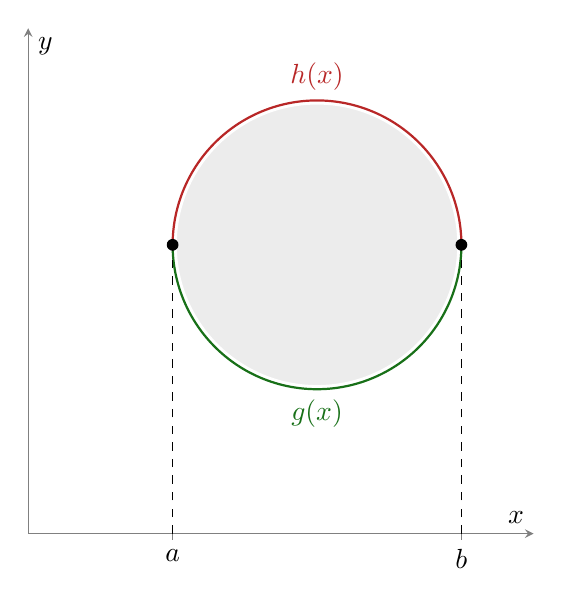
\begin{tikzpicture}
                \begin{axis}[
                        width = 8cm, height = 8cm,
                        xmin = 0, xmax = 3.5, ymin = 0, ymax = 3.5,
                        axis lines = middle,
                        xlabel = \normalsize $ x $, ylabel = \normalsize $ y $,
                        ymajorticks = false,
                        axis equal, xtick = {1, 3},
                        xticklabels = {\normalsize $ a $, \normalsize $ b $},
                        Ani]
                    \addplot[GraphSmooth, y_h, domain= pi : 2*pi, variable=\t]
                    ({2 + cos(\t)}, {2 + sin(\t)})
                    node[midway, below] {$ g(x) $};
                    \addplot[GraphSmooth, y_p, domain= 0 : pi, variable=\t]
                    ({2 + cos(\t)}, {2 + sin(\t)})
                    node[midway, above] {$ h(x) $};
                    \draw[dashed, black] (1, 0) -- (1, 2);
                    \draw[dashed, black] (3, 0) -- (3, 2);
                    \filldraw[draw = black!0, fill=gray!15](2, 2) circle (0.975);
                    \node[GraphNode] at (axis cs:1,2) {};
                    \node[GraphNode] at (axis cs:3,2) {};
                \end{axis}
            \end{tikzpicture}
        \end{figure}
        If the region $ R $ cannot be represented in the above form, it must at least be
        divisible into a finite number of areas that can.

    \item[Applications] The double integral of the unit function is simply
        the area enclosed by the boundary curves.
        \begin{align}
            \iint_R \dl A & = A_{\text{total}}
        \end{align}
        The volume beneath a surface $ z = f(x, y) > 0 $ and the $ xy $ plane is equal
        to its double integral over the area projected onto the $ xy $ plane.
        \begin{align}
            \iint_R f(x, y)\ \dl x\ \dl y = V
        \end{align}
        This is analogous to the area between the $ x $ axis and a one dimensional curve
        being its definite integral.

    \item[Change of variables] Starting with the single integral analog
        \begin{align}
            \int_{a}^{b}f(x) \dl x      & = \int_{\alpha}^{\beta}
            f\Big(x(u)\Big)\ \diff xu \dl u                       \\
            \iint_R f(x, y) \dl x \dl y & =
            \iint_{R^*} f\Big(x(u, v),\ y(u, v)\Big)\ \abs{J} \dl u \dl v
        \end{align}

    \item[Jacobian] A determinant that supplies the partial derivatives of each of the
        old variables w.r.t. each of the new variables.
        \begin{align}
            J & = \begin{vNiceMatrix}[r, margin]
                      \difcp xu & \difcp xv \\ \difcp yu & \difcp yv
                  \end{vNiceMatrix} =
            \diffp xu \ \diffp yv - \diffp xv \ \diffp yu
        \end{align}
        Assuming the functions $ x(u, v) $ and $ y(u, v) $ are continuous and have
        continuous first partial derivatives in some region $ R^* $ in the $ uv $ plane.

        \par There has to be a bijective mapping from $ (u, v) $ in $ R^* $ to $ (x, y) $
        in $ R $. The Jacobian has the same sign throughout $ R^* $

\end{description}

\section{Green's Theorem in the Plane}

\begin{description}
    \item[Utility] Converting a double integral over a region $ R $ into a line integral
        over its boundary in order to simplify computations.

    \item[Green' theorem] For a closed region $ R $ in 2 dimensions bounded by a finite
        number of smooth curves. Call this boundary $ C $. \par
        Let $ F_1(x, y) $ and $ F_2(x, y) $ be continuous functions in $ R $. Let the
        derivatives $ \difsp{F_1}{y} $ and $ \difsp{F_2}{x} $ also be continuous in a
        domain that is a superset of $ R $.

        \begin{align}
            \iint_R \left( \diffp{F_1}{y} - \diffp{F_2}{x} \right) \dl A & =
            \oint_C F_1 \dl x + F_2 \dl y                                    \\
            \iint (\nabla \times \vec{F}) \dotp \vec{k}\ \dl A           & =
            \oint_C \vec{F} \dotp \dl{\vec{r}}
        \end{align}
        The region $ R $ is to the left when moving along its boundary in order to
        preserve orientation. (in accordance with the direction of cross product)

    \item[Proof] General proof is complex and not covered here. For a specific kind of
        region $ R $ which can be represented by boundary curves in $ x $ or $ y $,
        \begin{align}
            \iint_R \diffp {F_1}{y}\ \dl A & = \int_{a}^{b} \Bigg[
            \int_{u(x)}^{v(x)} \diffp{F_1}{y}\ \dl y \Bigg]\ \dl x                   \\
                                           & = \int_{a}^{b} \Bigg[F_1
            \big( x, v(x) \big) - F_1 \big( x, u(x) \big) \Bigg] \dl x               \\
                                           & = -\int_{a}^{b} F_1 \big( x, u(x) \big)
            - \int_{b}^{a} F_1 \big( x, v(x) \big) = -\oint_C F_1 \big( x, y \big)
        \end{align}
        Since $ u(x) $ and $ v(x) $ both travel from $ x = a $ to $ x = b $, the above
        relation is a round trip starting and ending at $ x = a $, which reduces it
        to the closed line integral needed. \par
        A similar procedure for the closed region traversed from $ y = c $ to $ y = d $,
        via the two curves $ p(y) $ and $ q(y) $ gives the other half of the proof. \par

    \item[Area of region] Using Green's theorem to bypass the double integration,
        \begin{align}
            \iint_R \dl A & = \frac{1}{2} \oint_C \ (x \dl y) - (y \dl x) &
                          & \text{cartesian}                                \\
                          & = \frac{1}{2} \oint_C r^2 \dl \theta          &
                          & \text{polar}
        \end{align}

    \item[Normal derivative] Consider a scalar functionm $ w(x, y) $ that is continuous
        and has continuous first partial derivatives in the region $ R $.
        \begin{align}
            \vec{r}'               & = \diff {\vec{r}}{s} &
            \vec{r}' \dotp \vec{n} & = 0
        \end{align}
        Here, the parameter $ s $ is the arc length of the boundary curve. This ensures that
        the derivative $ \vec{r}' $ is the unit tangent vector. \par
        The outward facing vector perpendicular to $ \vec{r}' $ is the unit normal vector
        $ \vec{n} $. \par
        The component of the gradient along the unit normal vector is called the normal
        derivative.
        \begin{align}
            \nabla w \dotp \vec{n} = \diffp wn
        \end{align}

    \item[Relating Laplacian and normal derivative] Using the substitutions,
        \begin{align}
            F_1                       & = - \diffp wy               &
            F_2                       & = \diffp wx                   \\
            \iint_R \nabla^2 w\ \dl A & = \oint_C\ \diffp wn\ \dl s
        \end{align}
\end{description}

\section{Surfaces for Surface Integrals}

\begin{description}
    \item[Parametric representation] Similar to curves, surfaces can be parametrized
        using two parameters $ (u, v) $ to give
        \begin{align}
            \vec{r} & = \begin{bNiceMatrix}[margin]
                            x \\ y \\ z
                        \end{bNiceMatrix} \equiv
            \begin{bNiceMatrix}[margin]
                x(u, v) \\ y(y, v) \\ z(u, v)
            \end{bNiceMatrix}
        \end{align}
        This maps every point $ (u, v) $ in a region $ R $ of the $ uv $ plane onto
        the surface $ S $ in $ \mathcal{R}^3 $.

    \item[Tangent Plane] Consider one possible curve $ C $ on surface $ S $ that passes
        through a given point $ P $. \par
        Since the curve can be parametrized using a single parameter ($ t $), the chain
        rule gives,
        \begin{align}
            u,\ v                      & \equiv u(t),\ v(t)                  &
            \vec{\tilde{r}}(t)         & \equiv \vec{r}\Big(u(t),\ v(t)\Big)   \\
            \diff {\vec{\tilde{r}}}{t} & = \vec{\tilde{r}}'
            = \diffp {\vec{r}}{u}\ u'
            + \diffp {\vec{r}}{v}\ v'  &
            \vec{\tilde{r}}'           & = \vec{r}_u\ u' + \vec{r}_v\ v'
        \end{align}
        Here the functions $ u(t) $ and $ v(t) $ are continuous and have continuous
        derivatives w.r.t. $ t $.

    \item[Surface Normal vector] The partial derivatives are assumed L.I. and thus span
        the tangent plane at $ P $. Their cross product becomes the normal to the surface
        at $ P $
        \begin{align}
            \vec{N} & = \vec{r}_u \times \vec{r}_v \neq \vec{0}
        \end{align}
        Using the fact that the gradient of a level curve at a given point is the
        surface normal vector,
        \begin{align}
            g(x, y, z) = 0 \quad & \implies \quad \vec{N} = \nabla g
        \end{align}

    \item[Smooth surface] A surface whose normal vector depends continuously on the
        points of the surface.  \par
        At best, the surfaces encountered in practical applications can have a finite
        number of smooth portions.
\end{description}

\section{Surface Integrals}

\begin{description}
    \item[Parametrized surface integral] If the surface $ S $ is parametrized using
        the parameters $ u, v $which lie in region $ R $ of the $ uv $ plane, then,
        \begin{align}
            S :\ \vec{r}(u, v) & = \begin{bNiceMatrix}[margin]
                                       x(u, v) \\ y(u, v) \\ z(u, v)
                                   \end{bNiceMatrix}
        \end{align}
        This surface is piecewise smooth with a normal vector defined at every point.
        \begin{align}
            \vec{N}       & = \vec{r}_u \times \vec{r}_v                          &
            \vec{\hat{n}} & = \frac{\vec{N}}{\abs{\vec{N}}}                         \\
            \iint_S \vec{F} \dotp \vec{\hat{n}}
            \ \dl A       & = \iint_R \vec{F}(\vec{r}) \dotp \vec{N}\ \dl u \dl v
        \end{align}
        The area element of the actual surface $ \vec{\hat{n}}\ \dl A $ maps on to the
        area element $ \abs{\vec{N}} \dl u \dl v $ of the parameter plane $ R $.

    \item[Flux] In physics, the flux through a surface is the amount of some physical
        quantity (mass, heat) passing through the surface. \par
        It can mathematically be represented as the component of a vector field normal
        to the surface.
        \begin{align}
            \iint_S \vec{F} \dotp \vec{\hat{n}}\ \dl A &
            = \iint_S F_1\ \dl y \dl z + F_2\ \dl x \dl z + F_3\ \dl x \dl y
        \end{align}

    \item[Orientation of Surfaces] Changing the orientation of the surface (by choosing
        $ -\vec{n}$ instead of $ \vec{n} $), the value of the surface integral gets
        multiplied by $ -1 $.

    \item[Non-Orientable surface] Usually surfaces which have a positive direction of
        the normal vector at a given point $ P $ also have the same positive direction of
        the normal vector at all other points that can be reached by smoothly translating
        $ P $ along the surface. \par
        Surfaces like the Mobius strip are non-oreintable, because they do not satisfy
        this condition.

    \item[Surface Integral disregarding orientation] Consider a scalar function of
        position $ G(\vec{r}) $ to be integrated over a surface,
        \begin{align}
            \iint_S G(\vec{r})\ \dl A & = \iint_R G(\vec{r})\ \abs{\vec{N}}
            \ \dl u \dl v
        \end{align}
        Here, the normal vector and position vector are both parametrized using
        $ (u, v) $. \par
        One application is to find the mass of a surface, in which case the scalar
        function $ G(\vec{r}) $ is its area density. \par
        The total area of a surface $ A $ can be found using
        \begin{align}
            A & = \iint_S \dl A = \iint_R \abs{\vec{r}_u \times \vec{r}_v}\ \dl u \dl v
        \end{align}

    \item[Parametrization using coordinates] If the parameters chosen happen to be the
        $ x $ and $ y $ coordinates themselves, then,
        \begin{align}
            \vec{r}                   & = \begin{bNiceMatrix}[margin]
                                              x \\ y \\ f(x, y)
                                          \end{bNiceMatrix} \\
            \iint_S G(\vec{r})\ \dl A & = \iint_{R^*} G(x, y, f)\
            \Bigg[ \sqrt{1 + (\difcp fx)^2 + (\difcp fy)^2} \Bigg]\ \dl x \dl y
        \end{align}
        Here the parameter plane $ R^* $ is the $ xy $ plane and geometrically is the
        projection of the surface $ S $ onto the $ xy $ plane. \par
        By convention the normal vector points upwards away from the $ xy $ plane.

\end{description}

\section{Triple Integrals, Divergence Theorem of Gauss}

\begin{description}
    \item[Triple Integral] An integral over a closed, bounded $ 3d $ region in space.
        This volume is bounded by finitely many smooth surfaces. \par
        \begin{align}
            I & = \iiint_T\ f(x, y, z)\ \dl V
        \end{align}

    \item[Gauss' Divergence theorem] Triple integrals over a volume can be transformed
        into double integrals over the boundary surface using the divergence of the
        position vector,
        \begin{align}
            \vec{r}              & = \begin{bNiceMatrix}[margin]
                                         F_1 \\ F_2 \\ F_3
                                     \end{bNiceMatrix}                       &
            \nabla \dotp \vec{r} & = \diffp {F_1}{x} + \diffp{F_2}{y} + \diffp{F_3}{z}
        \end{align}
        For some continuous vector function $ \vec{F} $ in the region $ T $ which is
        continuous and has continuous first partial derivatives in some domain
        containing $ T $,
        \begin{align}
            \iiint_T\ \nabla \dotp F\ \dl V           &
            = \iint_S\ \vec{F} \dotp \vec{n}\ \dl S                        \\
            \iiint_T\ \Bigg[\diffp {F_1}{x} + \diffp{F_2}{y}
            + \diffp{F_3}{z}\Bigg]\ \dl x \dl y \dl z &
            = \iint_S\ F_1 \dl y \dl z + F_2 \dl x \dl z + F_3 \dl x \dl y \\
        \end{align}

    \item[Co-ordinate Invariance of divergence] Since the divergence is a scalar
        function of the position $ P $ in space, it is invariant under change of
        co-ordinate system.
        \begin{align}
            \nabla \dotp \vec{F}(P) & = \lim_{d(T) \rightarrow 0}
            \ \frac{1}{V(T)}\ \iint_{S(T)}\ \vec{F} \dotp \vec{n}\ \dl A
        \end{align}
        Here, $ V(T) $ is the volume of the region in space $ T $. \par
        $ S(T) $ is the boundary surface of the region $ T $.
        $ d(T) $ is the distance of the points in $ T $ from a specific point $ P $
        chosen in $ T $ to satisfy the mean value theorem for triple integrals.
\end{description}

\section{Further Applications of the Divergence Theorem}

\begin{description}
    \item[Fluid flow] Consider an incompressible fluid with density $ \rho = 1 $, with
        steady flow that does not varyin time. \par
        If the outward normal vector is $ \vec{n} $ and the fluid flow is characterized by
        the velocity field $ \vec{v} $, then
        \begin{align}
            \iint_S \vec{v} \dotp \vec{n}\ \dl A
        \end{align}
        represents the total mass of fluid flowing out of the region $ T $ bounded by the
        surface $ S $. \par
        There are no sources or sinks in a region $ T $ if and only if
        $ \nabla \dotp \vec{v} = 0$ everywhere in $ T $.

    \item[Heat equation] Since heat flows in the direction of decreasing temperature at a
        rate proportional to the gradient,
        \begin{align}
            \vec{v} & = -K\ \nabla U & \nabla \dotp \vec{v} & = -K\ \nabla^2 U
        \end{align}
        where $ U $ is the temperature, $ t $ is the time and $ K $ is the thermal
        conductivity of the body. \par
        Equating the rate of decrease of heat of the region $ T $ to the total heat
        flowing out of the bounding surface $ S $,
        \begin{align}
            \diffp Ut & = c^2\ \nabla^2 U
        \end{align}
        where $ c $ is the thermal diffusivity of the material. This equation is also
        called the diffusion equation.

    \item[Potential theory] Looking at solutions of Laplace's equation,
        \begin{align}
            \nabla^2 f & = \diff[2] fx + \diffp[2] fy + \diffp[2] fz = 0
        \end{align}
        Any solution of Laplace's equation $ f $ with continuous second-order partial
        derivatives is called a harmonic function.

    \item[Solutions of Laplace's equation] Using the definition of directional derivative
        to define the normal derivative in the direction of the outward normal,
        \begin{align}
            \diffp fn & \equiv \nabla f \dotp \vec{n}
        \end{align}
        If the underlying scalar function $ f $ is such that $ \vec{F} = \nabla f $,
        \begin{align}
            \iiint_T\ \nabla^2 f\ \dl V & = \iint_S\ \diffp fn\ \dl A
        \end{align}
        If $ f $ is a harmonic function then the integral of the normal derivative over
        the bounding surface $ S $ of some region in space $ T $ is zero.

    \item[Green's first formula] A special case of Green's theorem when the vector
        function $ \vec{F} $ is
        \begin{align}
            \vec{F}              & = f\ \nabla g                                 &
            \nabla \dotp \vec{F} & = f\ \nabla^2 g + (\nabla f) \dotp (\nabla g)
        \end{align}
        Substituting into Green's theorem gives,
        \begin{align}
            \iiint_T\ \Big[f\ \nabla^2 g + (\nabla f) \dotp (\nabla g)\Big]\ \dl V
             & = \iint_S \ f\ \diffp gn\ \dl A
        \end{align}

    \item[Green's second formula] An even more special case of Green's theorem, using
        the symmetry in Green's first formula upon interchange of $ f $ and $ g $.
        \begin{align}
            \iiint_T\ \Big[f\ \nabla^2 g - g\ \nabla^2 f \Big]\ \dl V
             & = \iint_S \ \left( f\ \diffp gn - g\ \diffp fn \right)\ \dl A
        \end{align}

    \item[Uniqueness of Harmonic functions] Let $ f $ be harmonic in some domain $ D $
        and equal to zero at every point of the bounding surface $ S $  of a region in
        space $ T $ as defined above. \par
        Then, $ f $ is identically zero in $ T $ \par
        This harmonic function $ f $ is uniquely determined in $ T $ by its values on the
        bounding surface $ S $
\end{description}

\section{Stokes' Theorem}

\begin{description}
    \item[Stokes' theorem] A generalization of Green's theorem in the plane to the full
        $ 3d $ space, using the curl. \par
        Consider a surface $ S $ whose bounding curve is parametrized using the arc length
        $ s $, with the outward normal unit vector being $ \vec{n} $
        \begin{align}
            \iint_R\ (\nabla \times \vec{F}) \dotp \vec{n}\ \dl A
             & = \oint_C\ \vec{F} \dotp \vec{r}'(s)\ \dl s
        \end{align}
        The unit tangent vector $ \vec{r}' $ is differentiated w.r.t. the arc length
        $ s $. \par
        The orientation of the curve is the same convention as for the cross product.
        \begin{align}
            \vec{n}\ \dl A  & = \vec{N}\ \dl u \dl v                      \\
            \vec{r}'\ \dl s & = \dl x \vec{\hat{i}} + \dl y \vec{\hat{j}}
            + \dl z \vec{\hat{k}}
        \end{align}
        In terms of the $ xyz $ coordinate system,
        \begin{align}
             & \iint_R \Bigg[\left( \diffp {F_3}{y} - \diffp{F_2}{z} \right) N_1
                + \left( \diffp {F_1}{z} - \diffp{F_3}{x} \right) N_2
                + \left( \diffp {F_2}{x} - \diffp{F_1}{y} \right) N_3\Bigg]
            \ \dl u \dl v                                                        \\
             & = \oint_C\ F_1\ \dl x + F_2\ \dl y + F_3\ \dl z
        \end{align}

    \item[Relation to Green's theorem] Green's theorem in the plane is a special case
        of Stokes' theorem,
        \begin{align}
            \vec{F}               & = \begin{bNiceMatrix}[margin]
                                          F_1 \\ F_2 \\ 0
                                      \end{bNiceMatrix}    &
            \nabla \times \vec{F} & =
            \begin{bNiceMatrix}[margin]
                -\difcp {F_2}{z} \\
                \difcp {F_1}{z}  \\
                \difcp {F_2}{x} - \difcp{F_1}{y}
            \end{bNiceMatrix}                          \\
            \vec{n}               & = \begin{bNiceMatrix}[margin]
                                          0 \\ 0 \\ 1
                                      \end{bNiceMatrix}    &
            \vec{r}'              & = \begin{bNiceMatrix}[margin]
                                          \dl x \\ \dl y \\ 0
                                      \end{bNiceMatrix}     \\
            \iint_S\ \Biggl( \diffp{F_2}{x} - \diffp{F_1}{y} \Biggr) \dl A
                                  & = \oint_C\ F_1 \dl x + F_2 \dl y
        \end{align}

    \item[Physical meaning of curl] Consider a disk of radius $ r_0 $ whose boundary
        is $ C_0 $ and the enlosed area is $ S_0 $,
        \begin{align}
            \oint_{C_0} \vec{v} \dotp \vec{r}'\ \dl s
             & = \iint_{S_0}\ (\nabla \times \vec{v}) \dotp \vec{n}\ \dl A \\
             & = \Big[(\nabla \times \vec{v}) \dotp \vec{n}\Big]_{Q}\ A_0
        \end{align}
        This is the $ 2d $ analog of the mean value theorem with the area of the disk
        $ A_0 $ and $ Q $ being some point in the area for which the equality holds.

        \begin{align}
            \Big[(\nabla \times \vec{v}) \dotp \vec{n}\Big]_Q
             & = \lim_{r_0 \rightarrow 0}
            \ \frac{1}{A_0}\ \oint_{C_0}\ \Biggl( \vec{v} \dotp \vec{r}'
            \Biggr)\ \dl s
        \end{align}
        If $ \vec{v} $ is the velocity vector, then the component of the curl in the
        outward normal direction can be visualized as a measure of the circulation of
        the fluid flow around the point $ Q $.

    \item[Path Independence] The proof for path independence of a line integral is
        straightforward using Stokes' theorem. \par
        Starting with the fact that the curl is zero, which means that the vector 
        function is the divergence of a scalar field, Stokes' theorem makes the 
        line integral over any closed path identically zero. \par
\end{description}
\chapter{Fourier Analysis}

\section{Fourier Series}

\begin{description}
    \item[Periodic function] A function defined on the real line, except possibly at a
        finite number of points such that,
        \begin{align}
            f(x + p)  & = f(x) & \forall\ x \in \mathcal{R} \\
            f(x + np) & =f(x)  & \forall\ n \in \mathcal{I}
        \end{align}
        for some positive real $ p $, which is called the period. \par
        The smallest positive period is called the fundamental period.

    \item[Trigonometric system] A family of periodic functions all having period $ 2\pi $
        which are the simplest basis used to represent all periodic functions.
        \begin{align}
            T & = \{1,\ \cos x,\ \sin x,\ \cos(2x),\ \sin(2x), \dots,\ \cos(nx),
            \ \sin(nx), \dots\}
        \end{align}

    \item[Fourier Series] A periodic function si represented as a linear combination of
        the above basis with each member assigned a coefficient (called the Fourier
        coefficient).
        \begin{align}
            f(x) & = a_0 + \iser[n]{0} a_n \cos(nx) + b_n \sin(nx)          \\
            a_0  & = \frac{1}{2\pi}\ \int_{-\pi}^{\pi} f(x)\ \dl x          \\
            a_n  & = \frac{1}{\pi}\ \int_{-\pi}^{\pi} f(x)\ \cos(nx)\ \dl x \\
            b_n  & = \frac{1}{\pi}\ \int_{-\pi}^{\pi} f(x)\ \sin(nx)\ \dl x
        \end{align}

    \item[Orthogonality of a trigonometric system] If integral over one period (taken to
        be $ -\pi $ to $ \pi $ by convention) of the product of any two members of the
        basis is zero, then the basis is orthogonal.
        \begin{align}
            \int_{-\pi}^{\pi}\ \cos(nx)\ \cos(mx)\ \dl x & = 0             &
            n                                            & \neq m            \\
            \int_{-\pi}^{\pi}\ \sin(nx)\ \sin(mx)\ \dl x & = 0             &
            n                                            & \neq m            \\
            \int_{-\pi}^{\pi}\ \cos(nx)\ \sin(mx)\ \dl x & = 0             &
            n,m                                          & \in \mathcal{I}
        \end{align}
        The Euler formulas for the Fourier coefficients are derived from the application
        of the orthogonality condition to the Fouier series definition.

    \item[Convergence of Fourier series] Let $ f(x) $ be periodic with period $ 2\pi $
        and be piecewise continuous in $ [-\pi, \pi] $. Also, let it have both
        left-handed and right-handed derivatives defined everywhere in this interval.
        \par Then, its Fourier series converges and is equal to $ f(x) $ at all points
        except at the finitely many points of discontinuity of $ f(x) $. \par
        At such points, the series converges to the average of the left and right-handed
        limits of $ f(x) $.
\end{description}

\section{Arbitrary Period, Even and Odd Functions, Half-Range Expansions}

\begin{description}
    \item[Functions with arbitrary period] Instead of the standard period $ p = 2\pi $,
        generalizing to $ p = 2L $ simply involves a change of variable
        \begin{align}
            2\pi \rightarrow 2L & \implies x \rightarrow \frac{\pi x}{L}    \\
            f(x)                & \rightarrow a_0 + \iser[n]{0} \Bigg[
                a_n\ \cos\left( \frac{n\pi x}{L} \right) +
            b_n\ \sin\left( \frac{n\pi x}{L} \right) \Bigg]                 \\
            a_0                 & = \frac{1}{2L}\ \int_{-L}^{L} f(x)\ \dl x \\
            a_n                 & = \frac{1}{L}\ \int_{-L}^{L}
            f(x)\ \cos\left( \frac{n\pi x}{L} \right) \dl x                 \\
            b_n                 & = \frac{1}{L}\ \int_{-L}^{L}
            f(x)\ \sin\left( \frac{n\pi x}{L} \right) \dl x
        \end{align}

    \item[Even and Odd functions] Even functions and odd functions can be
        represented just by a Fourier cosine and sine series respectively.
        \begin{align}
            f(-x) = f(x)  & \implies b_n = 0 \qquad \text{even}      \\
            f(-x) = -f(x) & \implies a_0 = a_n = 0 \qquad \text{odd}
        \end{align}

    \item[Lineraity] The Fourier series is linear under addition and scalar
        multiplication.
        \begin{align}
            f(x) + g(x) & \rightarrow F(x) + G(x) \\
            c\ f(x)     & \rightarrow c\ F(x)
        \end{align}
        Where the uppercase is the fourier series expansion of the lowercase function.

    \item[Half-range expansions] Extending the function specified in the domain
        $ [0, L] $ into the domain $ [-L, L] $ as either an even or odd function in order
        to simplify the computation of Fourier coefficients.
\end{description}

\section{Forced Oscillations}

\begin{description}
    \item[Standard form ODE] A second order linear ODE is very common in physical systems
        undergoing forced damped oscillations.
        \begin{align}
            my'' + cy' + ky = r(t)
        \end{align}
        Here, the output $ y(t) $ is the solution to the ODE, corresponding to the input
        $ r(t) $. The constant coefficients $ m, c, k $ characterize the system.

    \item[Solution to ODE] Since the input can be represented as a Fourier series,
        the output can also be decomposed into a sum of outputs corresponding to each
        input term. \par
        The amplitude of each of the output terms happens to be a function of the input
        frequency and typically, one or two frequencies dominate the output in most real
        world systems.
\end{description}

\section{Approximation by Trigonometric Polynomials}

\begin{description}
    \item[Trigonometric polynomial] An approximation of a function using a series of
        trigonometric functions. The fourier series expansion happens to be an example.
        \begin{align}
            f(x) & = A_0 + \iser[n]{1} \Big[ A_n \cos(nx) + B_n \sin(nx) \Big]
        \end{align}
        Here, $ N $ is called the order.

    \item[Square Error] The error in this approximation is
        \begin{align}
            E & = \int_{-\pi}^{\pi} (f - F)^2\ \dl x
        \end{align}
        This error is a measure of the agreement between the approximation $ f $ and
        the actual function $ F $ over the entire period of the trigonometric function.

    \item[Minimum square error] The squared error of a trigonometric polynomial
        $ F $ with fixed order $ N $ is smallest in the domainm $[-\pi, \pi] $ if the
        coefficients are the Fourier coefficients $ A_n = a_n, B_n = b_n $
        \begin{align}
            E^* & = \int_{-\pi}^{\pi} f^2\ \dl x  - \pi\ \Bigg[ 2a_0^2
                + \sum_{n=1}^{N} (a_n^2 + b_n^2) \Bigg]
        \end{align}
        The above squared error can only decrease with increasing $ N $.

    \item[Bessel's Inequality] Given a function $ f $ and fourier coefficients $ a_0,
            \{a_n\}, \{b_n\} $, the condition on minimized squared error gives,
        \begin{align}
            2a_0^2 + \iser[n]{1} (a_n^2 + b_n^2) & \leq \frac{1}{\pi}\ \int_{-\pi}^{\pi}
            \ f(x)^2\ \dl x
        \end{align}

    \item[Parseval's identity] The integral of the square of a function over its
        standardized period $ [-\pi, \pi] $ is equal to the sum of the squares of its
        Fourier coefficients. (rough analog of the Pythagoras theorem)
        \begin{align}
            2a_0^2 + \iser[n]{1} (a_n^2 + b_n^2) & = \frac{1}{\pi}\ \int_{-\pi}^{\pi}
            \ f(x)^2\ \dl x
        \end{align}
\end{description}

\section{Sturm-Liouville Problems, Orthogonal Functions}

\begin{description}
    \item[Sturm-Liouville problem] A second order ODE, along with boundary conditions
        of the form,
        \begin{align}
            \diff{}{x}\Bigg[p(x)\ \diff yx\Bigg] +
            \Bigg[ q(x) + \lambda r(x) \Bigg]y & = 0                         \\
            k_1 y + k_2 y'                     & = 0 \qquad \text{at}\ x = a \\
            l_1 y + l_2 y'                     & = 0 \qquad \text{at}\ x = b
        \end{align}
        for some interval $ x \in [a,b] $. $ \lambda $ is a paramter and the two
        $ k, l $ are real constants. \par
        If $ p,q,r,p' $ are real valued and continuous in the interval $ [a,b] $ and
        $ r $ is the same sign throughout, then all eigenvalues $ \lambda $ of the
        Sturm-Liouville equation are real.

    \item[Orthogonal functions] Using a weight function $ r(x) > 0 $, two functions
        are orthogonal in the interval $ x \in [a, b] $ if,
        \begin{align}
            (y_m, y_n) & = \int_{a}^{b} r(x)\ y_m(x)\ y_n(x)\ \dl x = 0 &
                       & \forall\quad m \neq n
        \end{align}

    \item[Norm of function] The square integral of the function $ f(x) $ with respect
        to the weight function $ r(x) $.
        \begin{align}
            \lVert y_n \rVert = \sqrt{(y_n, y_n)} &
            = \sqrt{\int_{a}^{b} r(x)\ y_n^2(x)\ \dl x}
        \end{align}

    \item[Orthonormal functions] A set of functions that are orthogonal in some interval
        $ x \in [a, b] $ and additionally all have unit norm. Using the Kronecker Delta
        functions,
        \begin{align}
            (y_m, y_n)  & = \int_{a}^{b} r(x)\ y_m(x)\ y_n(x)\ \dl x = \delta_{mn} \\
            \delta_{mn} & = \begin{dcases}
                                0 & \quad \text{if}\ m \neq n \\
                                1 & \quad \text{if}\ m = n    \\
                            \end{dcases}
        \end{align}
        The weight function is not mentioned when it is the identically equal to 1.

    \item[Eigenfunctions of Sturm-Lioville problems] Let $ y_m(x) $ and $ y_n(x) $ be
        eigenfunctions that correspond to different eigenvalues $ \lambda_m $ and
        $ \lambda_n $ of the Sturm-Liouville problem. \par
        Then, $ y_m, y_n $ are orthogonal on the interval $ [a, b] $ with respect to
        their weight function $ r(x) $ \par
        If $ p(a) = p(b) $, then the boundary conditions also become periodic,
        \begin{align}
            y(a) & = y(b) & y'(a) & = y'(b)
        \end{align}

    \item[Orthogonal system] Many real world systems can be cast into Sturm-Liouville
        form leading to a set of orthonormal basis functions. Examples include the Bessel
        functions, Legendre polynomials and Fourier series expansions.


\end{description}

%% section exercises
% \chapter{First Order ODEs}
\section{Basic Concepts: Modeling}

\begin{enumerate}
    \item Using the substitution $v = 2 \pi x$

          \begin{align}
              y' & = -2 \sin(2 \pi x)                     \\
              dy & = -2 \int \sin(2 \pi x) \quad dx       \\
              dy & = \frac{-1}{\pi} \int \sin(v) \quad dv \\
              y  & = \frac{\cos(2\pi x)}{\pi} + c
          \end{align}


    \item Using the substitution $v = -x^{2} / 2$

          \begin{align}
              y' & = -x \exp(-x^{2} / 2)                \\
              dy & = - \int x \exp(-x^{2} / 2) \quad dx \\
              dy & = \int \exp(v) \quad dv              \\
              y  & = \exp(-x^{2} / 2) + c
          \end{align}


    \item Using the integration over $y$

          \begin{align}
              y' & = y                         \\
              dx & = \int \frac{1}{y} \quad dy \\
              x  & = \ln(y) + c                \\
              y  & = C\exp(x)
          \end{align}


    \item Using the integration over $y$

          \begin{align}
              y' & = -1.5 y                      \\
              dx & = \int \frac{-2}{3y} \quad dy \\
              x  & = \frac{-2 \ln(y)}{3} + c     \\
              y  & = C\exp(-1.5x)
          \end{align}


    \item Using the substitution $v = 2 \pi x$

          \begin{align}
              y'            & = 4 e^{-x} \cos(x)                                                      \\
              \int \quad dy & = 4 \int e^{-x} \cos(x) \quad dx                                        \\
              y             & = 4 e^{-x} \sin(x)  + 4 \int e^{-x} \sin(x) \quad dx                    \\
              y             & = 4 e^{-x} \sin(x)  - 4 e^{-x} \cos(x) - 4 \int e^{-x} \cos(x) \quad dx \\
              y             & = 2 e^{-x} (\sin(x) - \cos(x))                                          \\
              y             & = -2 \sqrt{2} e^{-x} \cos\left(x + \frac{\pi}{4}\right) + c
          \end{align}


    \item Using the standard result for trigonometric ODEs, (second order ODE will result in two arbitrary constants)

          \begin{align}
              y'' & = -y                            \\
              y   & = c_{1} \cos(x) + c_{2} \sin(x)
          \end{align}


    \item Using the substitution $a  = 5.13$

          \begin{align}
              y'            & = \cosh(5.13 x)                             \\
              \int \quad dy & = \int \cosh(a x)  \quad dx                 \\
              y             & = \int \frac{e^{ax} + e^{-ax}}{2}  \quad dx \\
              y             & = \frac{\sinh(ax)}{a} + c
          \end{align}


    \item Using the substitution $a  = -0.2$ (Third order ODE results in 3 arbitrary constants)

          \begin{align}
              y''' & = \exp(-0.2x)                              \\
              y    & = \frac{\exp(ax)}{a^{3}} + bx^{2} + cx + d
          \end{align}


    \item IC is $y(0) = 2$

          \begin{align}
              4y      & = 4c\exp(-4x) + 1.4 \\
              y'      & =-4c \exp(-4x)      \\
              y' + 4y & = 1.4               \\
              y(0)    & = c + 0.35 = 2      \\
              c       & = 1.65
          \end{align}

          \begin{figure}[H]
              \centering
              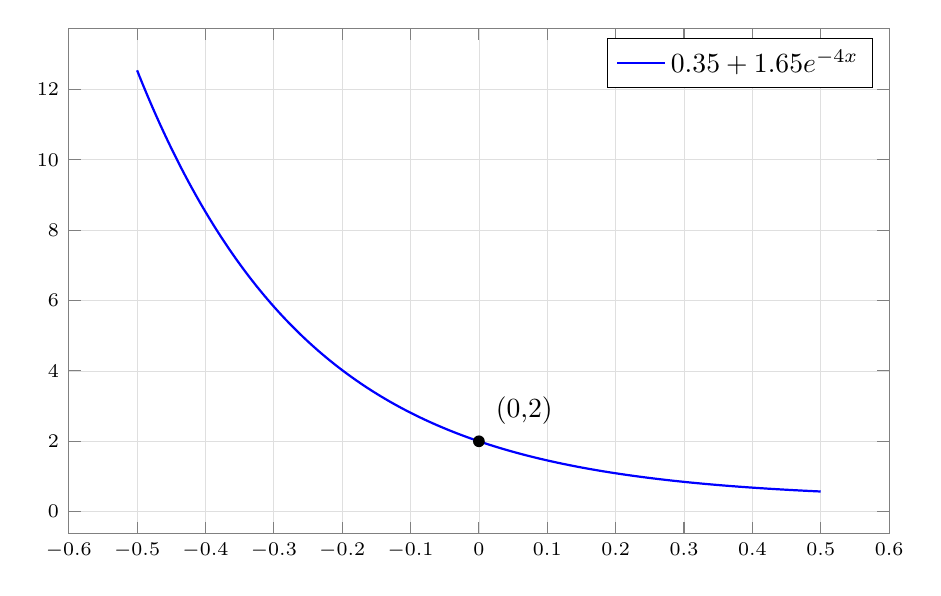
\begin{tikzpicture}
                  \begin{axis}[Ani, grid=both]
                      \addplot [GraphSmooth, domain=-0.5:0.5]
                      {0.35 + 1.65*e^(-4*x)};
                      \node[GraphNode, label={45:{(0,2)}}]
                      at (axis cs:0,2) {};
                      \addlegendentry{$0.35 + 1.65 e^{-4x}$}
                  \end{axis}
              \end{tikzpicture}
          \end{figure}

    \item IC is $y(0) = \pi$

          \begin{align}
              5xy      & = (5x) \ ce^{-2.5 x^{2}} \\
              y'       & = (-5x)\ ce^{-2.5 x^{2}} \\
              y' + 5xy & = 0                      \\
              y(0)     & = c  = \pi
          \end{align}

          \begin{figure}[H]
              \centering
              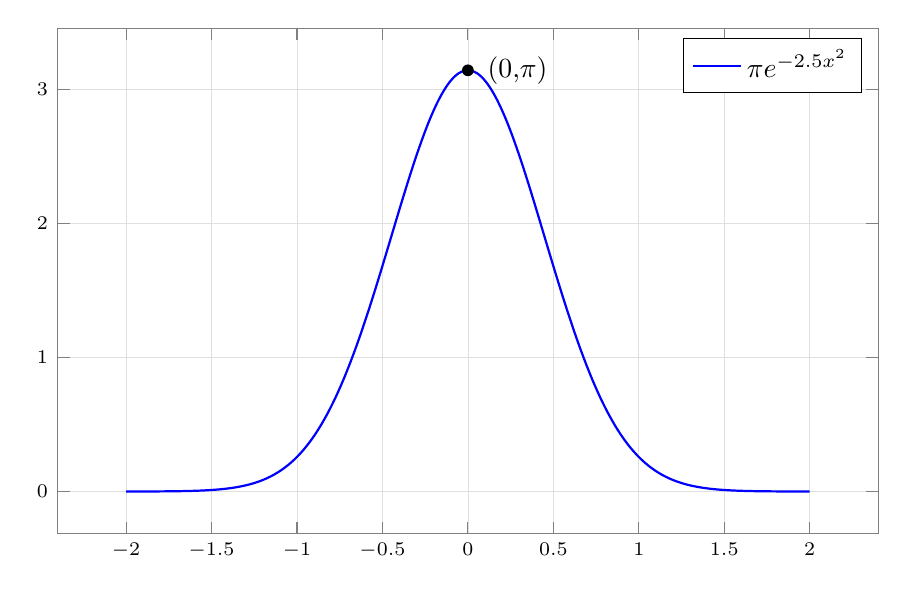
\begin{tikzpicture}
                  \begin{axis}[Ani, grid=both]
                      \addplot [GraphSmooth, domain=-2:2]
                      {pi * e^(-2.5 * x^(2))};
                      \node[GraphNode, label={0:{(0,$\pi$)}}]
                      at (axis cs:0,pi) {};
                      \addlegendentry{$\pi e^{-2.5x^{2}}$}
                  \end{axis}
              \end{tikzpicture}
          \end{figure}

    \item IC is $y(0) = 1/2$

          \begin{align}
              y'     & = (1 + x + c)\ e^{x} \\
              y' - y & = e^{x}              \\
              y(0)   & = c  = 1/2
          \end{align}

          \begin{figure}[H]
              \centering
              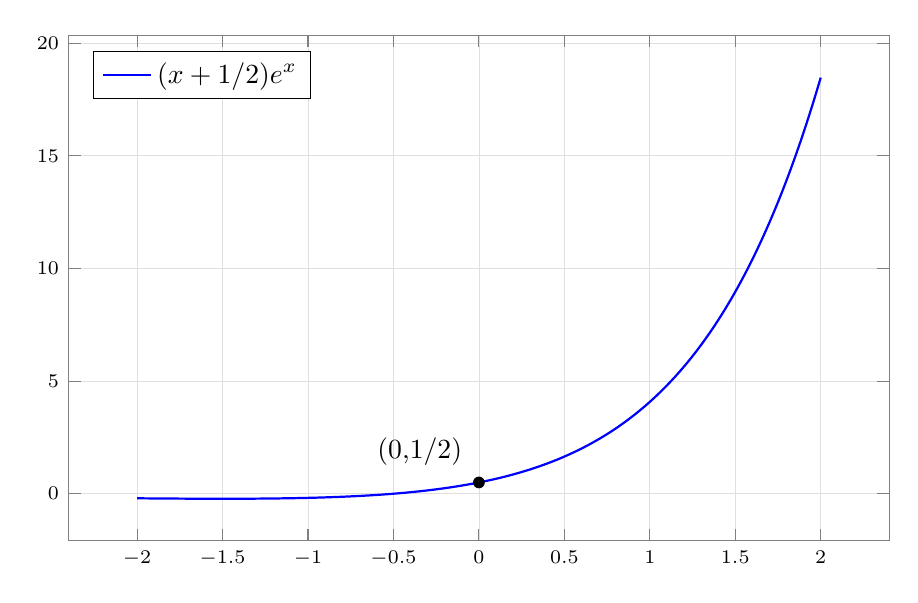
\begin{tikzpicture}
                  \begin{axis}[Ani, grid=both, legend pos = north west]
                      \addplot [GraphSmooth, domain=-2:2]
                      {(x + 0.5) * e^(x))};
                      \node[GraphNode, label={135:{(0,1/2)}}]
                      at (axis cs:0,1/2) {};
                      \addlegendentry{$(x + 1/2)e^{x}$}
                  \end{axis}
              \end{tikzpicture}
          \end{figure}

    \item IC is $y(1) = 4$

          \begin{align}
              2yy' & = 8x          & y & > 0 \\
              yy'  & = 4x          & y & > 0 \\
              y(1) & = c + 4  = 16           \\
              c    & = 12
          \end{align}

          \begin{figure}[H]
              \centering
              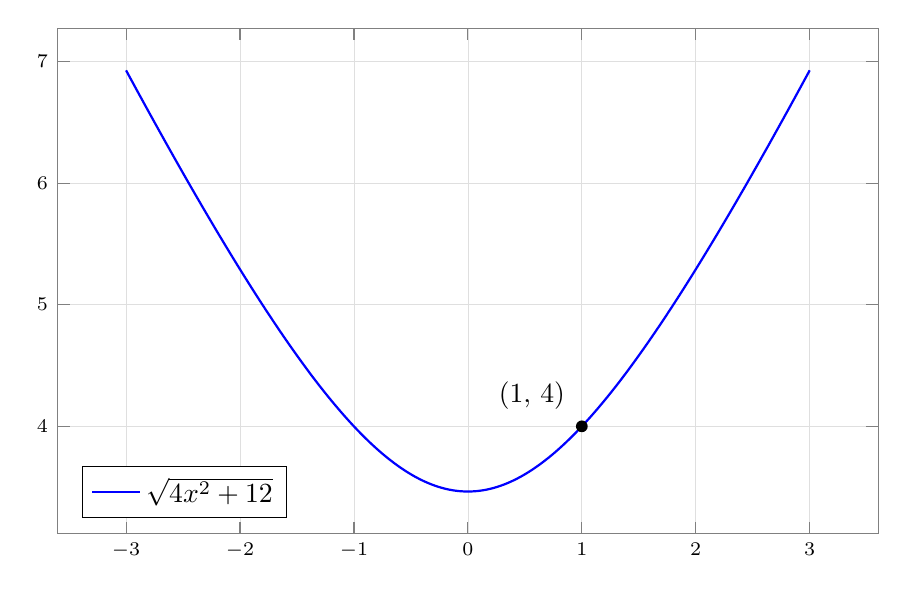
\begin{tikzpicture}
                  \begin{axis}[Ani, grid=both, legend pos = south west]
                      \addplot [GraphSmooth, domain=-3:3]
                      {(4*x^(2) + 12)^(1/2)};
                      \node[GraphNode, label={135:{(1, 4)}}]
                      at (axis cs:1, 4) {};
                      \addlegendentry{$\sqrt{4x^{2} + 12}$}
                  \end{axis}
              \end{tikzpicture}
          \end{figure}

    \item IC is $y(0) = 1/4$

          \begin{align}
              y'        & = \frac{ce^{-x}}{(1 + ce^{-x})^{2}}         \\
              y - y^{2} & = \frac{1 + ce^{-x} - 1}{(1 + ce^{-x})^{2}} \\
              y'        & = y - y^{2}                                 \\
              y(0)      & = \frac{1}{(1+c)}  = 1/4                    \\
              c         & = 3
          \end{align}

          \begin{figure}[H]
              \centering
              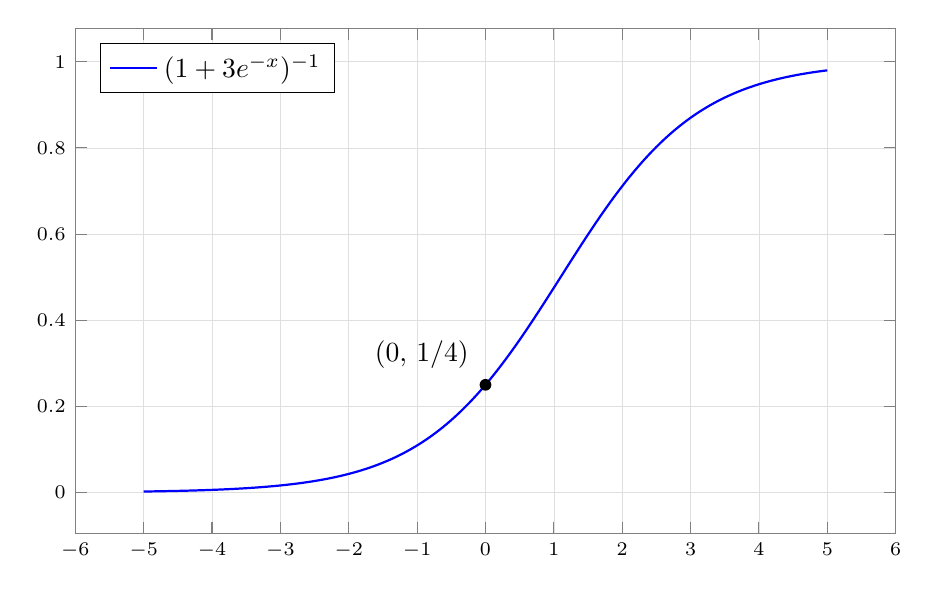
\begin{tikzpicture}
                  \begin{axis}[Ani, grid=both, legend pos = north west]
                      \addplot [GraphSmooth, domain=-5:5]
                      {1 / (1 + 3 * e^(-x))};
                      \node[GraphNode, label={135:{(0, 1/4)}}]
                      at (axis cs:0,1/4) {};
                      \addlegendentry{$(1 + 3e^{-x})^{-1}$}
                  \end{axis}
              \end{tikzpicture}
          \end{figure}

    \item IC is $y(\pi / 2) = 0$

          \begin{align}
              2y - 8     & = 2c\ \sin^{2} x              \\
              y' \tan x  & = 2c\ \sin x \ \cos x\ \tan x \\
              y' \tan x  & = 2y -  8                     \\
              y(\pi / 2) & = c + 4  = 0                  \\
              c          & = -4
          \end{align}

          \begin{figure}[H]
              \centering
              \begin{tikzpicture}
                  \begin{axis}[Ani, grid=both, legend pos = north east, PiStyleX]
                      \addplot [GraphSmooth, domain=-pi:pi]
                      {4 - 4*(sin(deg(x)))^(2)};
                      \node[GraphNode, label={0:{($\pi / 2$, 0)}}]
                      at (axis cs:pi/2, 0) {};
                      \addlegendentry{$-4 \sin^{2} x + 4$}
                  \end{axis}
              \end{tikzpicture}
          \end{figure}

    \item By Inspection , the ODE in Problem 13 has the constant solutions

          \begin{align}
              y & = 1 \\
              y & = 0
          \end{align}


    \item Verifying the general solution by substitution

          \begin{align}
              xy'    & = cx           \\
              y'^{2} & = c^{2}        \\
              y      & = cx - c^{2}   \\
              y      & = xy' - y'^{2}
          \end{align}

          Verifying the singular solution by substitution

          \begin{align}
              xy'    & = \frac{x^{2}}{2} \\
              y'^{2} & = \frac{x^{2}}{4} \\
              y      & = \frac{x^{2}}{4} \\
              y      & = xy' - y'^{2}
          \end{align}

          The parabola happens to have the same derivative for all $x$ as the member of the family of straight lines tangent to it. This makes the parabola a singular solution to the ODE.

    \item Given a starting mass of $1$ gm, find the time taken to reach a mass of $0.5$ gm. This is equal to half-life.

          \begin{align}
              \frac{dy}{dt} & = -ky                                                                           \\
              \ln y         & = -kt + c                                                                       \\
              y             & = c \ e^{-kt}                                                                   \\
              y_{T}         & = \frac{y_{0}}{2}                                                               \\
              e^{-kT}       & = 1/2                                                                           \\
              T             & = \frac{\ln 2}{k} = \frac{ln 2}{1.4 \times 10^{-11}} = 1568.89\  \mathrm{years}
          \end{align}


    \item Given the half life $ T = 3.6 $ days, in 1 day,

          \begin{align}
              y        & = c\ e^{-kt}                                               \\
              y(t = 1) & = c\ e^{-k} = y_{0} e ^{-k}                                \\
              y(t = 1) & = 1\ \mathrm{g} \times \exp \left(\frac{- \ln 2}{T}\right) \\
              y(t = 1) & = 0.825\ \mathrm{g}
          \end{align}
          and for 1 year,
          \begin{align}
              y(t = 365) & = c\ e^{-k} = y_{0} e ^{-365\ k}                                      \\
              y(t = 365) & = 1\ \mathrm{g} \times \exp \left(\frac{- \ln 2 \times 365}{T}\right) \\
              y(t = 365) & = 0\ \mathrm{g}
          \end{align}


    \item Given IC is $y(0) = 0$ and $y'(0) = 0$,

          \begin{align}
              \frac{d^{2}y}{dt^{2}} & = g                                            \\
              y                     & = a + bt + \frac{gt^{2}}{2}                    \\
              y(0)                  & = 0                         & \implies a & = 0 \\
              y'(0)                 & = 0                         & \implies b & = 0 \\
              y                     & = \frac{gt^{2}}{2}
          \end{align}


    \item Given IC is $y(18,000) = 1/2 \times y(0)$ and height $t$

          \begin{align}
              \frac{dy}{dt} & = -ky                                                     \\
              \ln y         & = -kt + c                                                 \\
              y             & = c \ e^{-kt}                                             \\
              y_{T}         & = \frac{y_{0}}{2}                                         \\
              e^{-kT}       & = 1/2                                                     \\
              k             & = \frac{\ln 2}{T} = \frac{ln 2}{18000}\  \mathrm{ft}^{-1} \\
              y(35,000)     & = y(0) \times 2^{-35/18}                                  \\
              y(35,000)     & = y(0) \times 0.259
          \end{align}

\end{enumerate}


\section{Geometric Meaning of y' = f(x, y)}

\begin{enumerate}
    \item Plotting direction field and curve passing through $(\pi / 4, 0)$

          \begin{align}
              y'         & = 1 + y^{2}                        &
              \dl x      & = \int \frac{1}{1 + y^{2}} \ \dl y   \\
              x          & = \arctan y + c                    &
              y          & = \tan(x + c)                        \\
              y(\pi / 4) & = \tan(\pi / 4 + c) = 0            &
              c          & = -\pi / 4
          \end{align}

          \begin{figure}[H]
              \centering
              \begin{tikzpicture}
                  \def\U{1}
                  \def\V{(1 + y^2)}
                  \def\LEN{sqrt(\U * \U + \V * \V)}
                  \begin{axis}[
                          PiStyleX, PiStyleY,
                          xtick distance = pi, ytick distance = pi,
                          legend pos = outer north east,
                          width = 8cm, Ani,
                          axis equal, domain = -2*pi:2*pi,
                          view = {0}{90},
                      ]
                      \addplot3 [forget plot,
                          color = gray!50,
                          point meta = {\LEN},
                          quiver={u={(\U) / \LEN},
                                  v={(\V) / \LEN},
                                  scale arrows = 0.5,},
                          -stealth,
                          samples=16,
                      ] (x, y, 0);
                      \addplot[GraphSmooth, y_h, restrict y to domain = -6.28:6.28]
                      {tan(x - pi/4)};
                      \addlegendentry{$ y' = \tan (x - \pi/4) $};
                  \end{axis}
              \end{tikzpicture}
          \end{figure}


    \item Plotting direction field and curve passing through $(1, 1)$ and $(0, 2)$

          \begin{align}
              y'               & = \frac{-4x}{y}       &
              \int -4x \ \dl x & = \int y \ \dl y        \\
              \frac{y^{2}}{2}  & = -2 x^{2} + c        &
              y^{2} + 4x^{2}   & = c                     \\
              c_{1}            & = 5 , \quad c_{2} = 4
          \end{align}

          \begin{figure}[H]
              \centering
              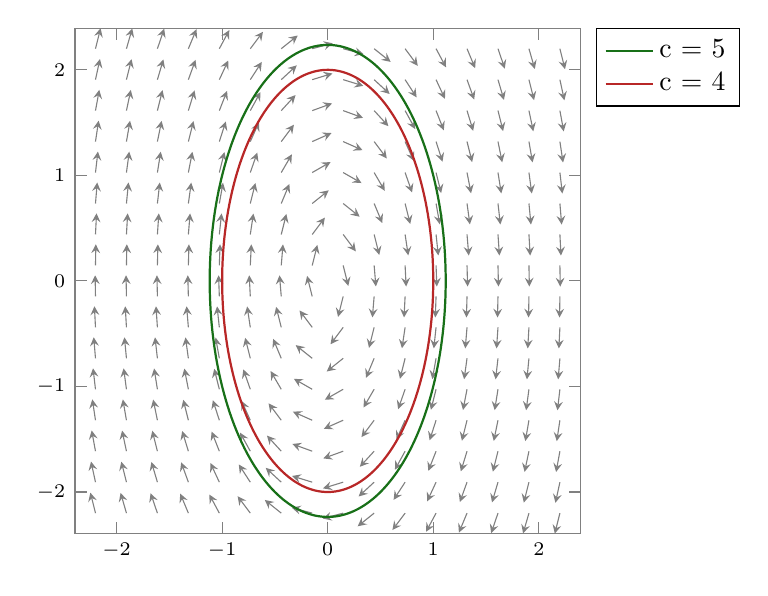
\begin{tikzpicture}
                  \def\U{y}
                  \def\V{-4*x}
                  \def\LEN{sqrt(\U * \U + \V * \V)}
                  \begin{axis}[
                          legend pos = outer north east,
                          width = 8cm,
                          height = 8cm,
                          Ani,
                          axis equal,
                          view     = {0}{90}, % for a view 'from above'
                      ]
                      \addplot3 [
                          forget plot,
                          domain = -2.2:2.2,
                          color = gray,
                          point meta = {\LEN},
                          quiver={u={(\U) / \LEN},
                                  v={(\V) / \LEN},
                                  scale arrows = 0.2,},
                          -stealth,
                          samples=16,
                      ] (x, y, 0);
                      \addplot [GraphSmooth, y_h, domain=-pi:pi, variable = \t]
                      ({sqrt(5/4) * cos(t)}, {sqrt(5) * sin(t)});
                      \addplot [GraphSmooth, domain=-pi:pi, variable = \t,
                          y_p]
                      ({sqrt(4/4) * cos(t)}, {sqrt(4) * sin(t)});
                      \addlegendentry{c = $5$};
                      \addlegendentry{c = $4$};
                  \end{axis}
              \end{tikzpicture}
          \end{figure}

    \item Plotting direction field and curve passing through $(0, 0)$ and $(2, 1/2)$

          \begin{align}
              y'          & = 1 - y^{2}                                      &
              \int\dl x   & = \int \frac{1}{1 - y^{2}} \ \dl y                 \\
              2 \int\dl x & = \int \frac{1}{1 + y} + \frac{1}{1 - y} \ \dl y &
              2x + a      & = \ln \left(\frac{1+y}{1-y}\right)                 \\
              y           & = \left(\frac{ce^{2x} - 1}{ce^{2x} + 1}\right)   &
              c_{1}       & = 1 , \quad c_{2} = \frac{3}{e^4}
          \end{align}

          \begin{figure}[H]
              \centering
              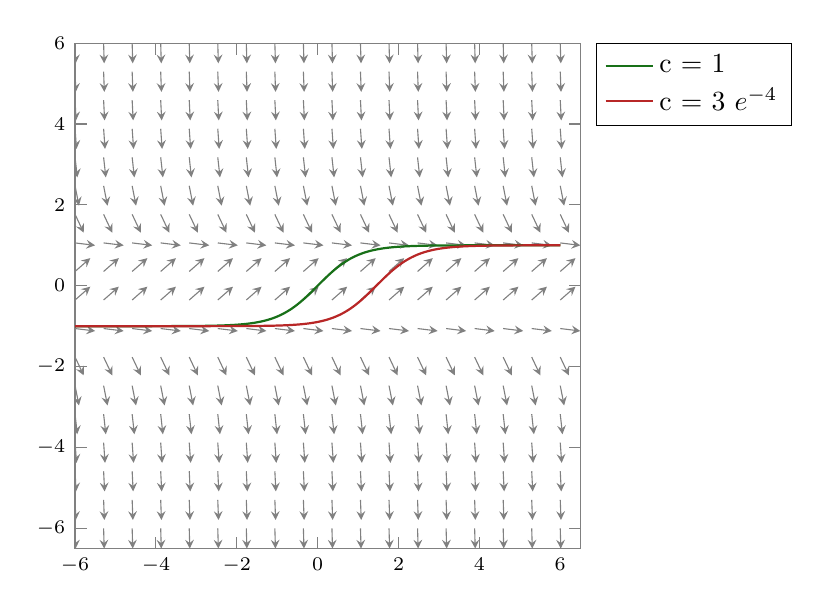
\begin{tikzpicture}
                  % \def\U{1}
                  % \def\V{1-y^(2)}
                  \def\LEN{sqrt(\U * \U + \V * \V)}
                  \begin{axis}[
                          legend pos = outer north east,
                          width = 8cm,
                          height = 8cm,
                          Ani,
                          axis equal,
                          view     = {0}{90}, % for a view 'from above'
                      ]
                      \addplot3 [
                          forget plot,
                          domain = -6:6,
                          color = gray,
                          quiver={
                                  %   u={(\U) / \LEN},
                                  %   v={(\V) / \LEN},
                                  u = 1 / sqrt(2 - 2 * y^2 + y^4),
                                  v = (1 - y^(2)) / sqrt(2 - 2 * y^2 + y^4),
                                  scale arrows = 0.5,},
                          -stealth,
                          samples=18,
                      ] (x, y, 0);
                      \addplot [GraphSmooth, y_h, domain=-6:6]
                      {(exp(2*x) - 1) / (exp(2*x) + 1)};
                      \addplot [GraphSmooth, domain=-6:6, y_p]
                      {((3 / exp(4))*exp(2*x) - 1) / ((3 / exp(4))*exp(2*x) + 1)};
                      \addlegendentry{c = $1$};
                      \addlegendentry{c = $3\ e^{-4}$};
                  \end{axis}
              \end{tikzpicture}
          \end{figure}

    \item Plotting direction field and curve passing through $(0, 0), (0, 1), (0, 2)$
          and $(0, 3)$

          \begin{align}
              y'                             & = 2y - y^{2}                          \\
              \int \ \dl x                   & = \int \frac{1}{y (2 - y)} \ \dl y    \\
              \int 2 \ \dl x                 & = \int \frac{1}{y} - \frac{1}{y - 2}
              \ \dl y                                                                \\
              \ln \left(\frac{y}{y-2}\right) & = 2 x + b                             \\
              y                              & = \frac{2c\ e^{2x}}{c\ e^{2x} - 1}    \\
              c_{1} = 0 , \quad c_{2}        & = -1, \quad c_{3} = \mathrm{singular}
              , \quad c_{4} = 1
          \end{align}

          \begin{figure}[H]
              \centering
              \begin{tikzpicture}
                  \def\U{1}
                  \def\V{y * (2 - y)}
                  \def\LEN{sqrt(\U * \U + \V * \V)}
                  \begin{axis}[
                          legend pos = outer north east,
                          width = 8cm,
                          height = 8cm,
                          Ani,
                          axis equal,
                          view     = {0}{90}, % for a view 'from above'
                      ]
                      \addplot3 [
                          forget plot,
                          domain = -5:5,
                          y domain = -4:6,
                          color = gray!50,
                          point meta = {\LEN},
                          quiver={u={(\U) / \LEN},
                                  v={(\V) / \LEN},
                                  scale arrows = 0.5,},
                          -stealth,
                          samples=20,
                      ] (x, y, 0);
                      \addplot [GraphSmooth, y_h, domain=-5:5]{0};
                      \addplot [GraphSmooth, domain=-5:5, y_p]{2};
                      \addplot [GraphSmooth, domain=-5:5, y_s]
                      {(2*e^(2*x)) / (1 + e^(2*x))};
                      \addplot [GraphSmooth, domain=0.2:5
                          , color = y_t]
                      {(2*e^(2*x)) / (e^(2*x) - 1)};
                      \addplot [GraphSmooth, domain=-5:-0.2
                          , color = y_t]
                      {(2*e^(2*x)) / (e^(2*x) - 1)};
                      \addlegendentry{c = $0$};
                      \addlegendentry{c = $-1$};
                      \addlegendentry{singular};
                      \addlegendentry{c = $1$};
                  \end{axis}
              \end{tikzpicture}
          \end{figure}

    \item Chini's equation
          %% Conpensating for the lack of any actual equations in this problem

    \item Plotting direction field and curve passing through $(0, -0.4)$ and $(0, 1)$

          \begin{align}
              y'           & = \sin^{2}y                           &
              \int \ \dl x & = \int \csc^{2} y \ \dl y               \\
              \tan y       & = \frac{-1}{x + c}                    &
              y            & = \arctan \left(\frac{-1}{x+c}\right)   \\
              c_{1}        & = \cot (0.4), \quad c_{2} = -\cot (1)
          \end{align}

          \begin{figure}[H]
              \centering
              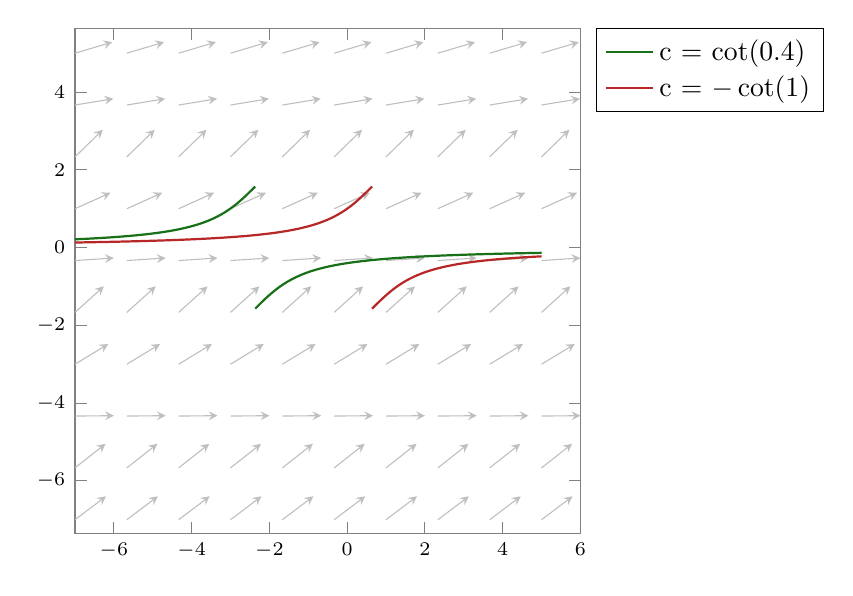
\begin{tikzpicture}
                  \def\U{1}
                  \def\V{sin(deg(y))^2}
                  \def\LEN{sqrt(\U * \U + \V * \V)}
                  \begin{axis}[
                          unbounded coords = jump,
                          legend pos = outer north east,
                          width = 8cm,
                          height = 8cm,
                          Ani,
                          axis equal,
                          view     = {0}{90}, % for a view 'from above'
                      ]
                      \addplot3 [
                          forget plot,
                          domain = -7:5,
                          color = gray!50,
                          point meta = {\LEN},
                          quiver={u={(\U) / \LEN},
                                  v={(\V) / \LEN},
                                  scale arrows = 1,},
                          -stealth,
                          samples=10,
                      ] (x, y, 0);
                      \addplot [GraphSmooth, y_h, domain=-7:-cot(0.4)]
                      {atan(-1/(x + cot(0.4)))};
                      \addplot [forget plot, GraphSmooth, y_h, domain=-cot(0.4):5]
                      {atan(-1/(x + cot(0.4)))};
                      \addplot [GraphSmooth, color = y_p, domain=-7:cot(1)]
                      {atan(-1/(x - cot(1)))};
                      \addplot [forget plot, GraphSmooth, color = y_p
                          , domain=cot(1):5]
                      {atan(-1/(x - cot(1)))};
                      \addlegendentry{c = $\cot (0.4)$};
                      \addlegendentry{c = $-\cot(1)$};
                  \end{axis}
              \end{tikzpicture}
          \end{figure}

    \item Plotting direction field and curve passing through $(2, 2)$ and $(3, 3)$,
          using the substitution $y = vx$

          \begin{align}
              y'            & = e^{y/x}                                         \\
              y'            & = e^{v} \qquad
              dv = -\frac{y}{x^{2}} \ \dl x                                     \\
              \int  \ \dl y & = x e^{y/x} - \int \frac{-y\ e^{y/x}}{x}  \ \dl x \\
              y             & = x e^{y/x} - \int \frac{y\ e^{v}}{v}  \ \dl v    \\
              y             & = x e^{y/x} - y\ \mathrm{Ei}(y/x) + c             \\
              c_{1}         & = 2 \mathrm{Ei}(1) - 2e, \quad c_{2}
              = 3 \mathrm{Ei}(1) - 3e
          \end{align}

          \begin{figure}[H]
              \centering
              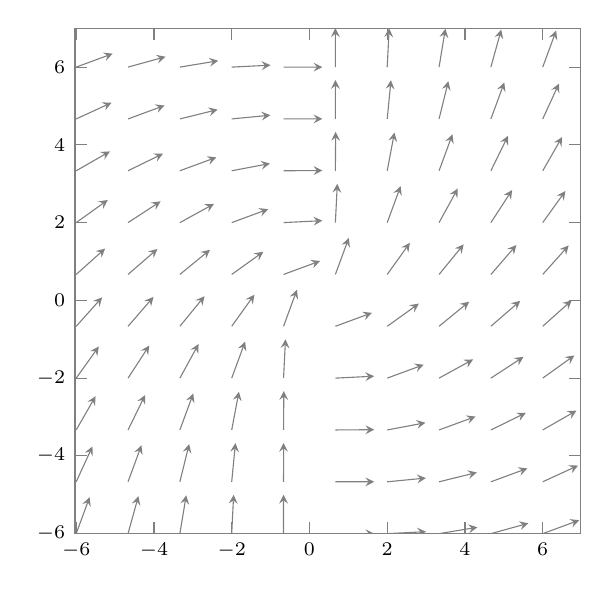
\begin{tikzpicture}
                  \def\U{1}
                  \def\V{e^(y/x)}
                  \def\LEN{sqrt(\U * \U + \V * \V)}
                  \begin{axis}[
                          unbounded coords = jump,
                          legend pos = outer north east,
                          width = 8cm,
                          height = 8cm,
                          Ani,
                          axis equal,
                          view     = {0}{90}, % for a view 'from above'
                      ]
                      \addplot3 [
                          forget plot,
                          domain = -6:6,
                          color = gray,
                          point meta = {\LEN},
                          quiver={u={(\U) / \LEN},
                                  v={(\V) / \LEN},
                                  scale arrows = 1,},
                          -stealth,
                          samples=10,
                      ] (x, y, 0);
                  \end{axis}
              \end{tikzpicture}
          \end{figure}

    \item Plotting direction field and curve passing through $(0, 1/2), (0, 1)$
          and $(0, 2)$

          \begin{align}
              y'                       & = -2xy                                  &
              \int \frac{1}{y} \ \dl y & = -2 \int x  \ \dl x                      \\
              \ln y                    & = -x^{2} + b                            &
              y                        & = c\ e^{-x^{2}}                           \\
              c_{1}                    & = 1/2, \quad c_{2} = 1, \quad c_{3} = 2
          \end{align}

          \begin{figure}[H]
              \centering
              \begin{tikzpicture}
                  \def\U{1}
                  \def\V{-2*x*y}
                  \def\LEN{sqrt(\U * \U + \V * \V)}
                  \begin{axis}[
                          unbounded coords = jump,
                          legend pos = outer north east,
                          width = 8cm,
                          height = 8cm,
                          Ani,
                          axis equal,
                          view     = {0}{90}, % for a view 'from above'
                      ]
                      \addplot3 [
                          forget plot,
                          domain = -3:3,
                          color = gray!50,
                          point meta = {\LEN},
                          quiver={u={(\U) / \LEN},
                                  v={(\V) / \LEN},
                                  scale arrows = 0.25,},
                          -stealth,
                          samples=16,
                      ] (x, y, 0);
                      \addplot [GraphSmooth, y_h, domain=-3:3]
                      {0.5 * e^(-1* x * x)};
                      \addplot [GraphSmooth, domain=-3:3, color = y_p]
                      {1 * e^(-1* x * x)};
                      \addplot [GraphSmooth, domain=-3:3, color = y_t]
                      {2 * e^(-1* x * x)};
                      \addlegendentry{c = $1/2$};
                      \addlegendentry{c = $1$};
                      \addlegendentry{c = $2$};
                  \end{axis}
              \end{tikzpicture}
          \end{figure}

    \item Plotting direction field and curve passing through $(0, 1/2), (0, 1)$
          and $(0, 2)$

          \begin{align}
              y' & = \cos (\pi x)                    &
              y  & = \frac{1}{\pi}\ \sin (\pi x) + c
          \end{align}

          \begin{figure}[H]
              \centering
              \begin{tikzpicture}
                  \def\U{1}
                  \def\V{cos(pi * x)}
                  \def\LEN{sqrt(\U * \U + \V * \V)}
                  \begin{axis}[
                          unbounded coords = jump,
                          legend pos = outer north east,
                          width = 8cm,
                          height = 8cm,
                          Ani,
                          axis equal,
                          view     = {0}{90}, % for a view 'from above'
                      ]
                      \addplot3 [
                          forget plot,
                          domain = -2:2,
                          color = gray!50,
                          point meta = {\LEN},
                          quiver={u={(\U) / \LEN},
                                  v={(\V) / \LEN},
                                  scale arrows = 0.2,},
                          -stealth,
                          samples=16,
                      ] (x, y, 0);
                      \addplot [GraphSmooth, y_h, domain=-2:2]
                      {(1/pi) * sin(pi * x)};
                      \addplot [GraphSmooth, y_p, domain=-2:2]
                      {(1/pi) * sin(pi * x) + 1};
                      \addplot [GraphSmooth, y_t, domain=-2:2]
                      {(1/pi) * sin(pi * x) - 1};
                      \addlegendentry{c = $0$};
                      \addlegendentry{c = $1$};
                      \addlegendentry{c = $-1$};
                  \end{axis}
              \end{tikzpicture}
          \end{figure}

    \item Plotting direction field and curve passing through $(0, 1/2), (0, 1)$
          and $(0, 2)$

          \begin{align}
              y'       & = -5y^{1/2} &
              \sqrt{y} & = -2.5x + c
          \end{align}

          \begin{figure}[H]
              \centering
              \begin{tikzpicture}
                  \def\U{1}
                  \def\V{-5 * y^(1/2)}
                  \def\LEN{sqrt(\U * \U + \V * \V)}
                  \begin{axis}[
                          unbounded coords = jump,
                          legend pos = outer north east,
                          width = 8cm,
                          height = 8cm,
                          Ani,
                          axis equal,
                          view     = {0}{90}, % for a view 'from above'
                      ]
                      \addplot3 [
                          forget plot,
                          domain = -1:0,
                          y domain = 0:1,
                          color = gray!50,
                          point meta = {\LEN},
                          quiver={u={(\U) / \LEN},
                                  v={(\V) / \LEN},
                                  scale arrows = 0.05,},
                          -stealth,
                          samples=16,
                      ] (x, y, 0);
                      \addplot [GraphSmooth, y_h, domain=-1:0,
                          restrict y to domain=0:1]
                      ({x}, {(-2.5  * x)^(2)});
                      \addplot [GraphSmooth, y_p, domain=-1:0,
                          restrict y to domain=0:1]
                      ({x}, {(-2.5  * x -1)^(2)});
                      \addplot [GraphSmooth, y_t, domain=-1:0,
                          restrict y to domain=0:1]
                      ({x}, {(-2.5  * x - 0.2)^(2)});
                      \addlegendentry{c = $0$};
                      \addlegendentry{c = $-1$};
                      \addlegendentry{c = $-0.2$};
                  \end{axis}
              \end{tikzpicture}
          \end{figure}

    \item Isoclines with an ODE of the form $y' = f(y)$ will be of the form $f(y) = c$.
          These are straight lines parallel to the x axis.

    \item Plotting direction field and curve passing through $(0, 2)$

          \begin{align}
              vy             & = 2             &
              \int y \ \dl y & = 2\int \ \dl t   \\
              y^{2}          & = 4t + c        &
              y(0)           & = \sqrt{c} = 2    \\
              y              & =\sqrt{4t + 4}
          \end{align}

          \begin{figure}[H]
              \centering
              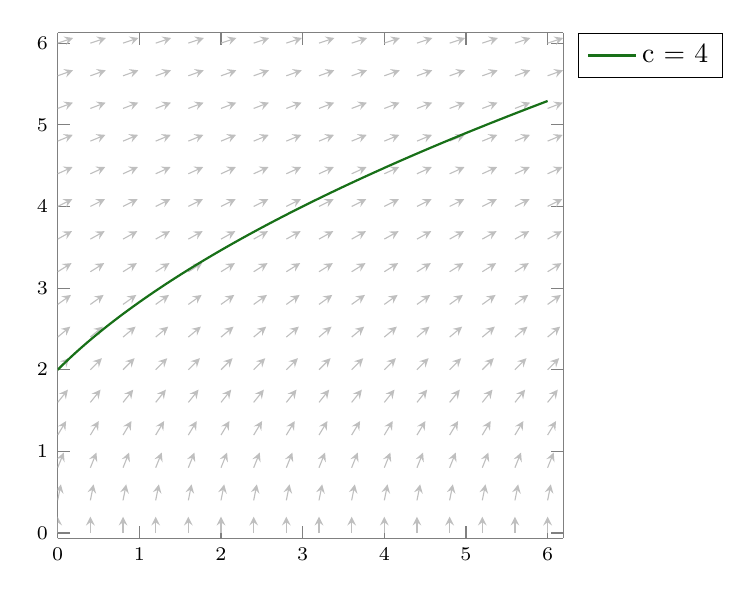
\begin{tikzpicture}
                  \def\U{y}
                  \def\V{2}
                  \def\LEN{sqrt(\U * \U + \V * \V)}
                  \begin{axis}[
                          unbounded coords = jump,
                          legend pos = outer north east,
                          width = 8cm,
                          height = 8cm,
                          Ani,
                          axis equal,
                          view     = {0}{90}, % for a view 'from above'
                      ]
                      \addplot3 [
                          forget plot,
                          domain = 0:6,
                          y domain = 0:6,
                          color = gray!50,
                          point meta = {\LEN},
                          quiver={u={(\U) / \LEN},
                                  v={(\V) / \LEN},
                                  scale arrows = 0.2,},
                          -stealth,
                          samples=16,
                      ] (x, y, 0);
                      \addplot [GraphSmooth, y_h, domain=0:6]
                      {(4*x + 4)^(1/2)};
                      \addlegendentry{c = $4$};
                  \end{axis}
              \end{tikzpicture}
          \end{figure}

    \item Plotting direction field and curve passing through $(1, 1)$

          \begin{align}
              y                        & = vt                       &
              \int \frac{1}{y} \ \dl y & = \int \frac{1}{t} \ \dl t   \\
              \ln y                    & = \ln t + b                &
              y                        & = ct                         \\
              c                        & = 1
          \end{align}

          \begin{figure}[H]
              \centering
              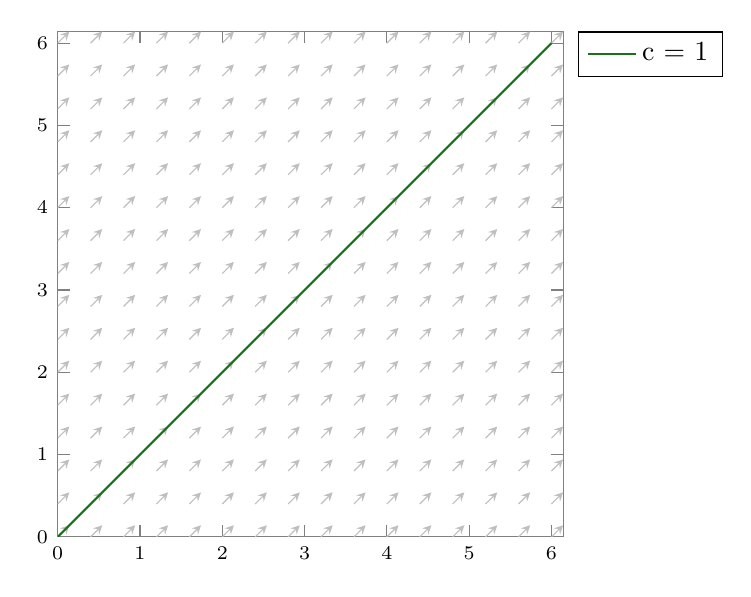
\begin{tikzpicture}
                  \def\U{1}
                  \def\V{1}
                  \def\LEN{sqrt(\U * \U + \V * \V)}
                  \begin{axis}[
                          unbounded coords = jump,
                          legend pos = outer north east,
                          width = 8cm,
                          height = 8cm,
                          Ani,
                          axis equal,
                          view     = {0}{90}, % for a view 'from above'
                      ]
                      \addplot3 [
                          forget plot,
                          domain = 0:6,
                          color = gray!50,
                          point meta = {\LEN},
                          quiver={u={(\U) / \LEN},
                                  v={(\V) / \LEN},
                                  scale arrows = 0.2,},
                          -stealth,
                          samples=16,
                      ] (x, y, 0);
                      \addplot [GraphSmooth, y_h, domain=0:6]
                      {x};
                      \addlegendentry{c = $1$};
                  \end{axis}
              \end{tikzpicture}
          \end{figure}

    \item Plotting direction field and curve passing through $(0, 1/\sqrt{2})$

          \begin{align}
              y^{2} + v^{2}                          & = 1                &
              \diff yt                               & = \sqrt{1 - y^{2}}   \\
              \int \frac{1}{\sqrt{1- y^{2}}} \ \dl y & = \int\ \dl t      &
              \arcsin y                              & = t + c              \\
              y                                      & = \sin (t + c)     &
              c                                      & = \frac{\pi}{4}
          \end{align}

          \begin{figure}[H]
              \centering
              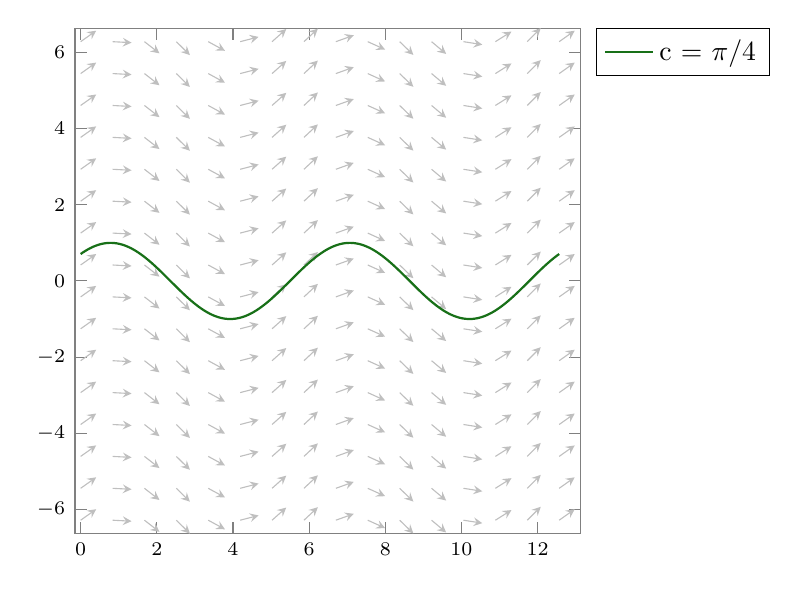
\begin{tikzpicture}
                  \def\U{1}
                  \def\V{cos(x + 0.25 * pi)}
                  \def\LEN{sqrt(\U * \U + \V * \V)}
                  \begin{axis}[
                          unbounded coords = jump,
                          legend pos = outer north east,
                          width = 8cm,
                          height = 8cm,
                          Ani,
                          axis equal,
                          view     = {0}{90}, % for a view 'from above'
                      ]
                      \addplot3 [
                          forget plot,
                          domain = 0 : 4 * pi,
                          y domain = -2 * pi : 2 * pi,
                          color = gray!50,
                          point meta = {\LEN},
                          quiver={u={(\U) / \LEN},
                                  v={(\V) / \LEN},
                                  scale arrows = 0.5,},
                          -stealth,
                          samples=16,
                      ] (x, y, 0);
                      \addplot [GraphSmooth, y_h, domain=0:4*pi]
                      {sin(x + 0.25 * pi)};
                      \addlegendentry{c = $\pi / 4$};
                  \end{axis}
              \end{tikzpicture}
          \end{figure}

    \item Plotting direction field given $m = k = 1$ and $v_{0} = 10$ and drag
          proportional to $v^{2}$. \\
          Terminal velocity is $v^{T} = \sqrt{g} = 3.13\ m/s^{2}$

          \begin{align}
              my''                            & = mv' = mg - kv^{2}                   \\
              \int \frac{1}{g - v^{2}}\ \dl v & = \int \ \dl t                        \\
              \frac{1}{2 \sqrt{g}}
              \int \frac{1}{\sqrt{g} - v}
              + \frac{1}{\sqrt{g} + v}
              \ \dl v                         & = \int \ \dl t                        \\
              \ln \left(\frac{v + \sqrt{g}}
              {v - \sqrt{g}}\right)           & = 2 \sqrt{g} t + b                    \\
              v                               & = \sqrt{g}
              \ \frac{c\ \exp(2 \sqrt{g}t) + 1}{c\ \exp(2 \sqrt{g}t) - 1}             \\
              c                               & = \frac{10 + \sqrt{g}}{10 - \sqrt{g}}
          \end{align}
          \begin{figure}[H]
              \centering
              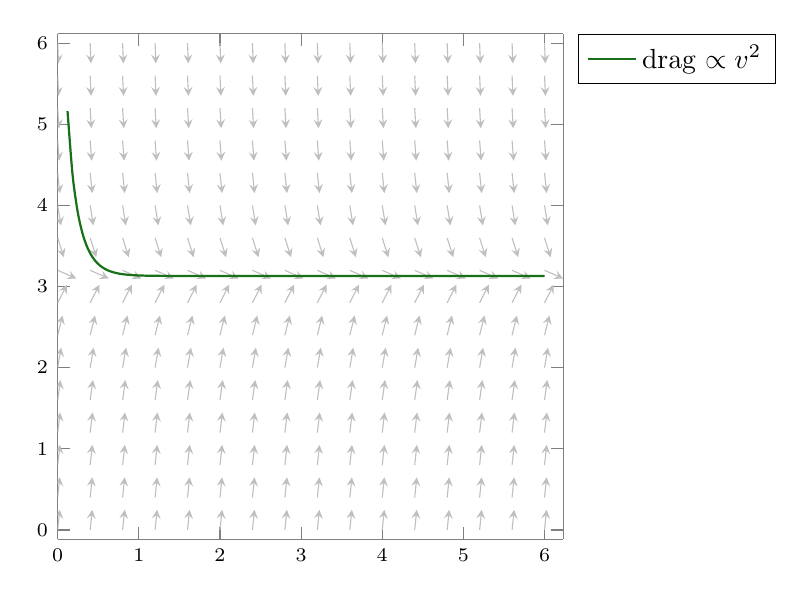
\begin{tikzpicture}
                  \def\U{1}
                  \def\V{-1 * (y^(2) - 9.8)}
                  \def\LEN{sqrt(\U * \U + \V * \V)}
                  \def\c{(10 + (9.8)^(1/2)) / (10 - (9.8)^(1/2))}
                  \begin{axis}[
                          unbounded coords = jump,
                          legend pos = outer north east,
                          width = 8cm,
                          height = 8cm,
                          Ani,
                          axis equal,
                          view     = {0}{90}, % for a view 'from above'
                      ]
                      \addplot3 [
                          forget plot,
                          domain = 0 : 6,
                          y domain = 0  : 6 ,
                          color = gray!50,
                          point meta = {\LEN},
                          quiver={u={(\U) / \LEN},
                                  v={(\V) / \LEN},
                                  scale arrows = 0.25,},
                          -stealth,
                          samples=16,
                      ] (x, y, 0);
                      \addplot [GraphSmooth, y_h, domain=0:6, samples = 100,
                          restrict y to domain = 0:6]
                      {sqrt(9.8) * (\c * e^(2 * sqrt(9.8) * x) + 1)
                          / (\c * e^(2 * sqrt(9.8) * x) - 1)};
                      \addlegendentry{drag $\propto v^{2}$};
                  \end{axis}
              \end{tikzpicture}
          \end{figure}

          Plotting direction field given $m = k = 1$ and $v_{0} = 10$ and drag
          proportional to $v$. \\
          Terminal velocity is $v^{T} = g = 9.8\ m/s^{2}$
          \begin{align}
              my''                             & = mv' = mg - kv   \\
              \int \frac{1}{g - v}\ \dl v      & = \int \ \dl t    \\
              \ln \left(\frac{1}{v - g}\right) & = t + b           \\
              v                                & = g + c e^{-t}    \\
              c                                & = v_{0} - g = 0.2
          \end{align}

          \begin{figure}[H]
              \centering
              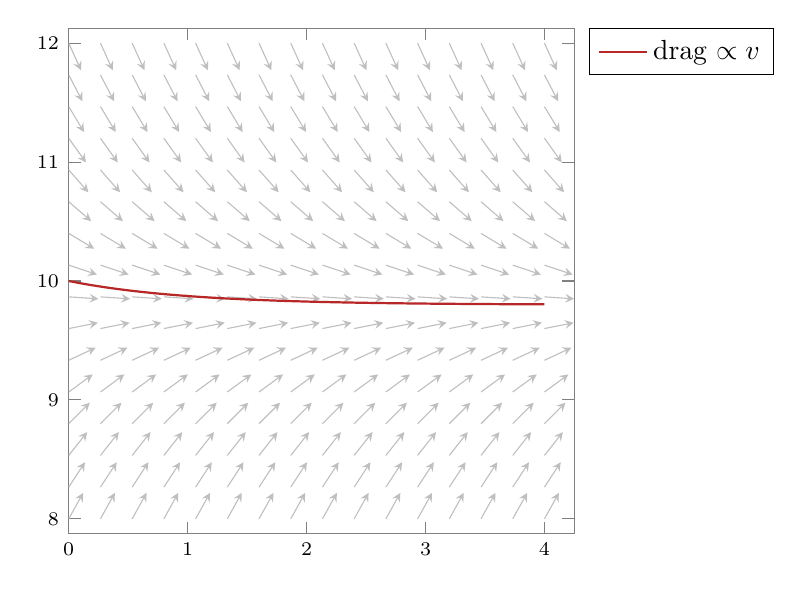
\begin{tikzpicture}
                  \def\U{1}
                  \def\V{-1 * (y - 9.8)}
                  \def\LEN{sqrt(\U * \U + \V * \V)}
                  \begin{axis}[
                          unbounded coords = jump,
                          legend pos = outer north east,
                          width = 8cm,
                          height = 8cm,
                          Ani,
                          axis equal,
                          view     = {0}{90}, % for a view 'from above'
                      ]
                      \addplot3 [
                          forget plot,
                          domain = 0 : 4,
                          y domain = 8  : 12 ,
                          color = gray!50,
                          point meta = {\LEN},
                          quiver={u={(\U) / \LEN},
                                  v={(\V) / \LEN},
                                  scale arrows = 0.25,},
                          -stealth,
                          samples=16,
                      ] (x, y, 0);
                      \addplot [GraphSmooth, domain=0:4, y_p]
                      {9.8 + 0.2 * e^(-x)};
                      \addlegendentry{drag $\propto v$};
                  \end{axis}
              \end{tikzpicture}
          \end{figure}

    \item CAS Project using the ODE $y' = y + x$
          \begin{enumerate}
              \item Zooming in the regions $x \in [-5, 2]$ shows the upper part
                    of the solutions which increase for large $x$ \\
                    Zooming in the regions $y \in [-1, 5]$ shows the lower part
                    of the solutions which decreases for large $x$, as well as the
                    straight line unstable equilibrium solution

                    \begin{figure}[H]
                        \centering
                        \begin{subfigure}[b]{0.49\textwidth}
                            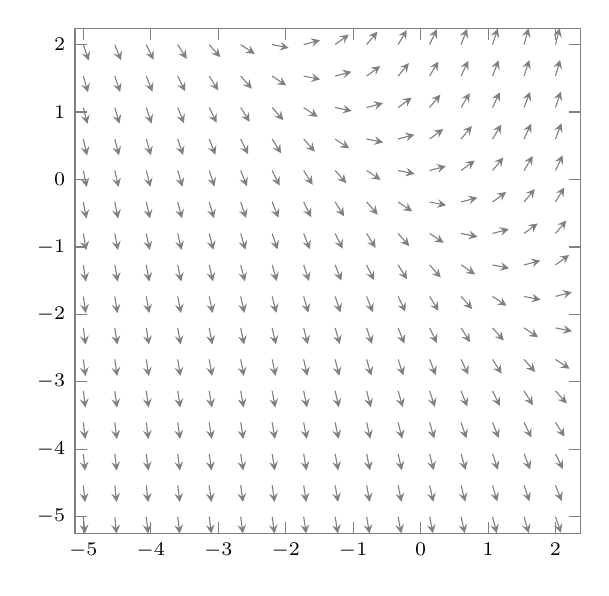
\begin{tikzpicture}
                                \def\U{1}
                                \def\V{(x + y)}
                                \def\LEN{sqrt(\U * \U + \V * \V)}
                                \begin{axis}[
                                        unbounded coords = jump,
                                        legend pos = outer north east,
                                        width = 8cm,
                                        height = 8cm,
                                        Ani,
                                        axis equal,
                                        view     = {0}{90}, % for a view 'from above'
                                    ]
                                    \addplot3 [
                                        forget plot,
                                        domain = -5 : 2,
                                        color = gray,
                                        point meta = {\LEN},
                                        quiver={u={(\U) / \LEN},
                                                v={(\V) / \LEN},
                                                scale arrows = 0.25,},
                                        -stealth,
                                        samples=16,
                                    ] (x, y, 0);
                                \end{axis}
                            \end{tikzpicture}
                        \end{subfigure}
                        \hfill
                        \begin{subfigure}[b]{0.49\textwidth}
                            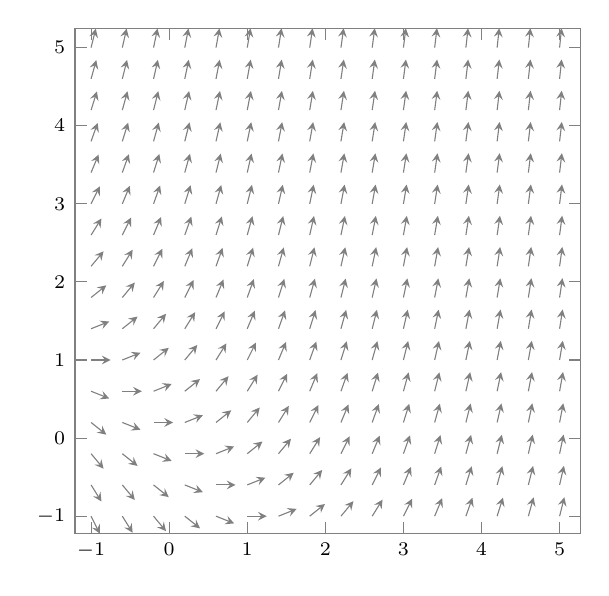
\begin{tikzpicture}
                                \def\U{1}
                                \def\V{(x + y)}
                                \def\LEN{sqrt(\U * \U + \V * \V)}
                                \begin{axis}[
                                        unbounded coords = jump,
                                        legend pos = outer north east,
                                        width = 8cm,
                                        height = 8cm,
                                        Ani,
                                        axis equal,
                                        view     = {0}{90}, % for a view 'from above'
                                    ]
                                    \addplot3 [
                                        forget plot,
                                        domain = -1:5,
                                        restrict y to domain = -1:5,
                                        color = gray,
                                        point meta = {\LEN},
                                        quiver={u={(\U) / \LEN},
                                                v={(\V) / \LEN},
                                                scale arrows = 0.25,},
                                        -stealth,
                                        samples=16,
                                    ] (x, y, 0);
                                \end{axis}
                            \end{tikzpicture}
                        \end{subfigure}
                    \end{figure}
              \item Implicit differentiation gives the ODE

                    \begin{align}
                        x^{2} + 9y^{2} & = c \quad (y > 0)             \\
                        x + 9yy'       & = 0                           \\
                        y'             & = \frac{-x}{9y} \quad (y > 0)
                    \end{align}
                    The sign of the RHS determine whether the direction field is
                    an ellipse or a hyperbola. A special case of the RHS being
                    $-x/y$ gives a circle (a special ellipse)

                    \begin{figure}[H]
                        \centering
                        \begin{subfigure}[b]{0.49\textwidth}
                            \centering
                            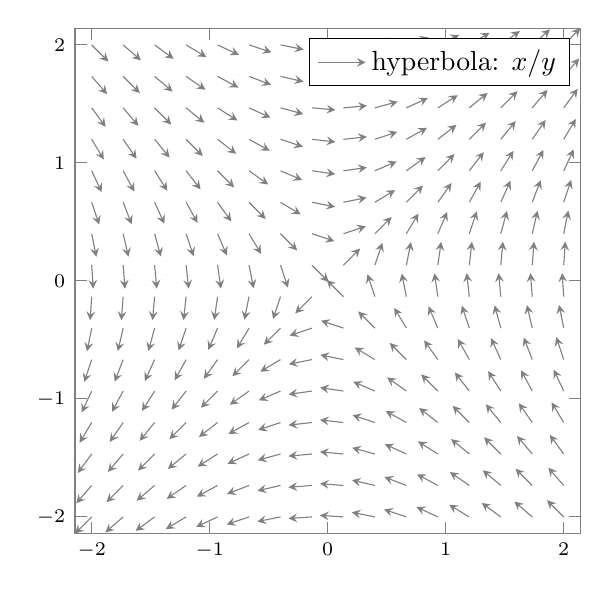
\begin{tikzpicture}
                                \def\U{y}
                                \def\V{x}
                                \def\LEN{sqrt(\U * \U + \V * \V)}
                                \begin{axis}[
                                        unbounded coords = jump,
                                        width = 8cm,
                                        height = 8cm,
                                        Ani,
                                        axis equal,
                                        view     = {0}{90}, % for a view 'from above'
                                    ]
                                    \addplot3 [
                                        domain = -2 : 2,
                                        restrict y to domain = -2:2,
                                        color = gray,
                                        point meta = {\LEN},
                                        quiver={u={(\U) / \LEN},
                                                v={(\V) / \LEN},
                                                scale arrows = 0.2,},
                                        -stealth,
                                        samples=16,
                                    ] (x, y, 0);
                                    \addlegendentry{hyperbola: $x/y$};
                                \end{axis}
                            \end{tikzpicture}
                        \end{subfigure}
                        \hfill
                        \begin{subfigure}[b]{0.49\textwidth}
                            \centering
                            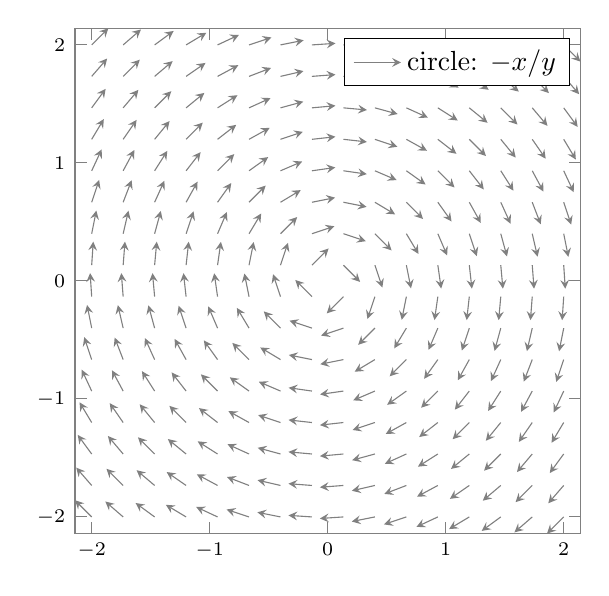
\begin{tikzpicture}
                                \def\U{y}
                                \def\V{-x}
                                \def\LEN{sqrt(\U * \U + \V * \V)}
                                \begin{axis}[
                                        unbounded coords = jump,
                                        width = 8cm,
                                        height = 8cm,
                                        Ani,
                                        axis equal,
                                        view     = {0}{90}, % for a view 'from above'
                                    ]
                                    \addplot3 [
                                        domain = -2 : 2,
                                        restrict y to domain = -2:2,
                                        color = gray,
                                        point meta = {\LEN},
                                        quiver={u={(\U) / \LEN},
                                                v={(\V) / \LEN},
                                                scale arrows = 0.2,},
                                        -stealth,
                                        samples=16,
                                    ] (x, y, 0);
                                    \addlegendentry{circle: $-x/y$};
                                \end{axis}
                            \end{tikzpicture}
                        \end{subfigure}
                        \vskip\baselineskip
                        \begin{subfigure}[b]{0.49\textwidth}
                            \centering
                            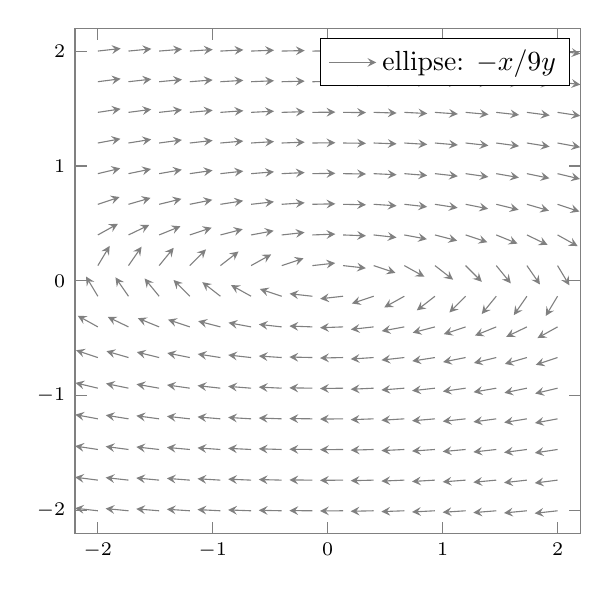
\begin{tikzpicture}
                                \def\U{9*y}
                                \def\V{-x}
                                \def\LEN{sqrt(\U * \U + \V * \V)}
                                \begin{axis}[
                                        unbounded coords = jump,
                                        width = 8cm,
                                        height = 8cm,
                                        Ani,
                                        axis equal,
                                        view     = {0}{90}, % for a view 'from above'
                                    ]
                                    \addplot3 [
                                        domain = -2 : 2,
                                        restrict y to domain = -2:2,
                                        color = gray,
                                        point meta = {\LEN},
                                        quiver={u={(\U) / \LEN},
                                                v={(\V) / \LEN},
                                                scale arrows = 0.2,},
                                        -stealth,
                                        samples=16,
                                    ] (x, y, 0);
                                    \addlegendentry{ellipse: $-x/9y$};
                                \end{axis}
                            \end{tikzpicture}
                        \end{subfigure}
                        \hfill
                        \begin{subfigure}[b]{0.49\textwidth}
                            \centering
                            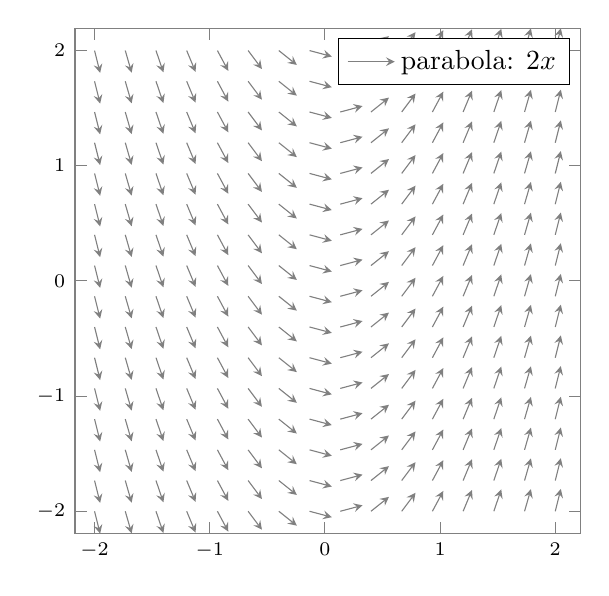
\begin{tikzpicture}
                                \def\U{1}
                                \def\V{2*x}
                                \def\LEN{sqrt(\U * \U + \V * \V)}
                                \begin{axis}[
                                        unbounded coords = jump,
                                        width = 8cm,
                                        height = 8cm,
                                        Ani,
                                        axis equal,
                                        view     = {0}{90}, % for a view 'from above'
                                    ]
                                    \addplot3 [
                                        domain = -2 : 2,
                                        color = gray,
                                        point meta = {\LEN},
                                        quiver={u={(\U) / \LEN},
                                                v={(\V) / \LEN},
                                                scale arrows = 0.2,},
                                        -stealth,
                                        samples=16,
                                    ] (x, y, 0);
                                    \addlegendentry{parabola: $2x$};
                                \end{axis}
                            \end{tikzpicture}
                        \end{subfigure}
                    \end{figure}
              \item From the figure above, $y' = -x/y$ produces a circle
              \item For the ODE $y' = -y/2$
                    \begin{align}
                        y'    & = \frac{-1}{2y} \\
                        y^{2} & = -x + c
                    \end{align}

                    For $y > 0$, the solutions decrease because the ODE is
                    monotonically negative for all $y > 0$.
                    \begin{figure}[H]
                        \centering
                        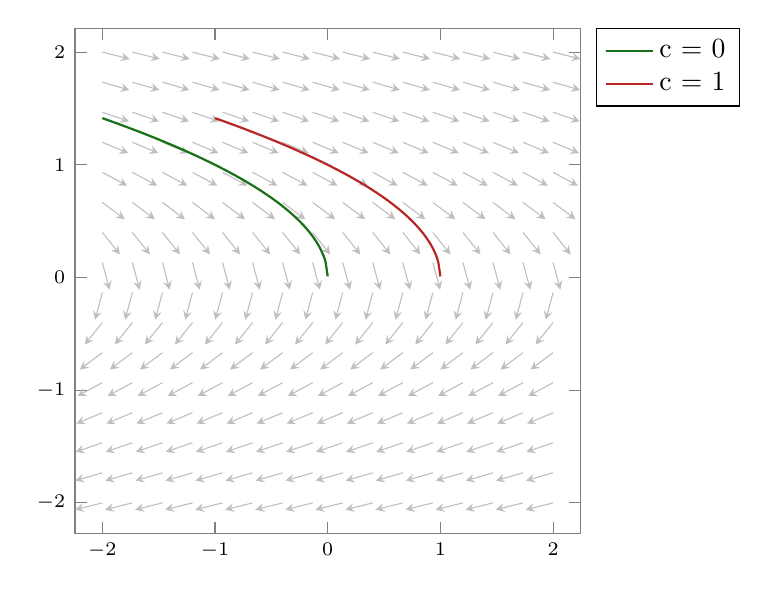
\begin{tikzpicture}
                            \def\U{y}
                            \def\V{(-0.5)}
                            \def\LEN{sqrt(\U * \U + \V * \V)}
                            \begin{axis}[
                                    unbounded coords = jump,
                                    legend pos = outer north east,
                                    width = 8cm,
                                    height = 8cm,
                                    Ani,
                                    axis equal,
                                    view     = {0}{90}, % for a view 'from above'
                                ]
                                \addplot3 [
                                    forget plot,
                                    domain = -2:2,
                                    color = gray!50,
                                    point meta = {\LEN},
                                    quiver={u={(\U) / \LEN},
                                            v={(\V) / \LEN},
                                            scale arrows = 0.25,},
                                    -stealth,
                                    samples=16,
                                ] (x, y, 0);
                                \addplot [GraphSmooth, y_h, domain=-2:0,
                                    samples = 100]
                                {sqrt(-x)};
                                \addlegendentry{c = $0$};
                                \addplot [GraphSmooth, y_p, domain=-1:1,
                                    samples = 100]
                                {sqrt(-x + 1)};
                                \addlegendentry{c = $1$};
                            \end{axis}
                        \end{tikzpicture}
                    \end{figure}
          \end{enumerate}

    \item Euler's method with $y(0) = 1$ and step size $h = 0.1$

          \begin{align}
              y' & = y      &
              y  & = ce^{x}   \\
              c  & = 1
          \end{align}

          \begin{figure}[H]
              \centering
              \begin{tikzpicture}
                  \begin{axis}[
                          grid = both,
                          legend pos = north west,
                          unbounded coords = jump,
                          width = 12cm,
                          height = 12cm,
                          Ani,
                      ]
                      \addplot[
                          only marks,]
                      table [
                              x index =1,
                              y index =2,
                              col sep=comma]
                          {./tables/table_01_01_17.csv};
                      \addplot [
                          forget plot,
                          GraphSmooth,
                          domain=0:1]
                      {e^(x)};
                      \addlegendentry{numerical};
                      \addplot[
                          only marks,
                          color = red,
                          mark = square]
                      table [
                              x index =1,
                              y index =3,
                              col sep=comma]
                          {./tables/table_01_01_17.csv};
                      \addlegendentry{exact};
                  \end{axis}
              \end{tikzpicture}
          \end{figure}

    \item Euler's method with $y(0) = 1$ and step size $h = 0.01$

          \begin{align}
              y' & = y      &
              y  & = ce^{x}   \\
              c  & = 1
          \end{align}

          \begin{figure}[H]
              \centering
              \begin{tikzpicture}
                  \begin{axis}[
                          xticklabel style={
                                  /pgf/number format/fixed,
                                  /pgf/number format/precision=5
                              },
                          grid = both,
                          legend pos = north west,
                          unbounded coords = jump,
                          width = 8cm,
                          height = 8cm,
                          Ani,
                      ]
                      \addplot[
                          only marks,]
                      table [
                              x index =1,
                              y index =2,
                              col sep=comma]
                          {./tables/table_01_01_18.csv};
                      \addplot [
                          forget plot,
                          GraphSmooth,
                          domain=0:0.1]
                      {e^(x)};
                      \addlegendentry{numerical};
                      \addplot[
                          only marks,
                          color = red,
                          mark = square]
                      table [
                              x index =1,
                              y index =3,
                              col sep=comma]
                          {./tables/table_01_01_18.csv};
                      \addlegendentry{exact};
                  \end{axis}
              \end{tikzpicture}
          \end{figure}

    \item Euler's method with $y(0) = 0$ and step size $h = 0.1$

          \begin{align}
              y' & = (y - x)^{2} &
              y  & = x - \tanh x
          \end{align}

          \begin{figure}[H]
              \centering
              \begin{tikzpicture}
                  \begin{axis}[
                          grid = both,
                          legend pos = north west,
                          unbounded coords = jump,
                          width = 12cm,
                          height = 12cm,
                          Ani,
                      ]
                      \addplot[
                          only marks,]
                      table [
                              x index =1,
                              y index =2,
                              col sep=comma]
                          {./tables/table_01_01_19.csv};
                      \addplot [
                          forget plot,
                          GraphSmooth,
                          domain=0:1]
                      {x - tanh(x)};
                      \addlegendentry{numerical};
                      \addplot[
                          only marks,
                          color = red,
                          mark = square]
                      table [
                              x index =1,
                              y index =3,
                              col sep=comma]
                          {./tables/table_01_01_19.csv};
                      \addlegendentry{exact};
                  \end{axis}
              \end{tikzpicture}
          \end{figure}

    \item Euler's method with $y(0) = 1$ and step size $h = 0.2$

          \begin{align}
              y' & = -5x^{4}y^{2}          &
              y  & = \frac{1}{(c + x^{5})}   \\
              c  & = 1
          \end{align}

          \begin{figure}[H]
              \centering
              \begin{tikzpicture}
                  \begin{axis}[
                          grid = both,
                          legend pos = north east,
                          unbounded coords = jump,
                          width = 12cm,
                          height = 12cm,
                          Ani,
                      ]
                      \addplot[
                          only marks,]
                      table [
                              x index =1,
                              y index =2,
                              col sep=comma]
                          {./tables/table_01_01_20.csv};
                      \addplot [
                          forget plot,
                          GraphSmooth,
                          domain=0:2]
                      {(1 + x^5)^(-1)};
                      \addlegendentry{numerical};
                      \addplot[
                          only marks,
                          color = red,
                          mark = square]
                      table [
                              x index =1,
                              y index =3,
                              col sep=comma]
                          {./tables/table_01_01_20.csv};
                      \addlegendentry{exact};
                  \end{axis}
              \end{tikzpicture}
          \end{figure}

\end{enumerate}
\section{Separable ODEs. Modeling}

\begin{enumerate}
    \item Adding the constant of integration later might result in a vastly
          different general solution which is almost always wrong.

    \item Using $u = y/x$. Then substituting $(1 + u^{4}) = m$

          \begin{align}
              y'                     & = \frac{-x^{3}}{y^{3}} = \frac{-1}{u^{3}}     \\
              \frac{\dl u}{f(u) - u} & =  \frac{\dl x}{x} = \frac{-u^{3}\ \dl u}
              {1 + u^{4}}                                                            \\
              \ln (|x|) + b          & = \int \frac{-\dl m}{4m} = \frac{-1}{4} \ln m \\
              1 + \left(\frac{y}{x}\right)^{4}
                                     & = \frac{c}{x^{4}}                             \\
              y^{4}                  & = c - x^{4}
          \end{align}
          \begin{figure}[H]
              \centering
              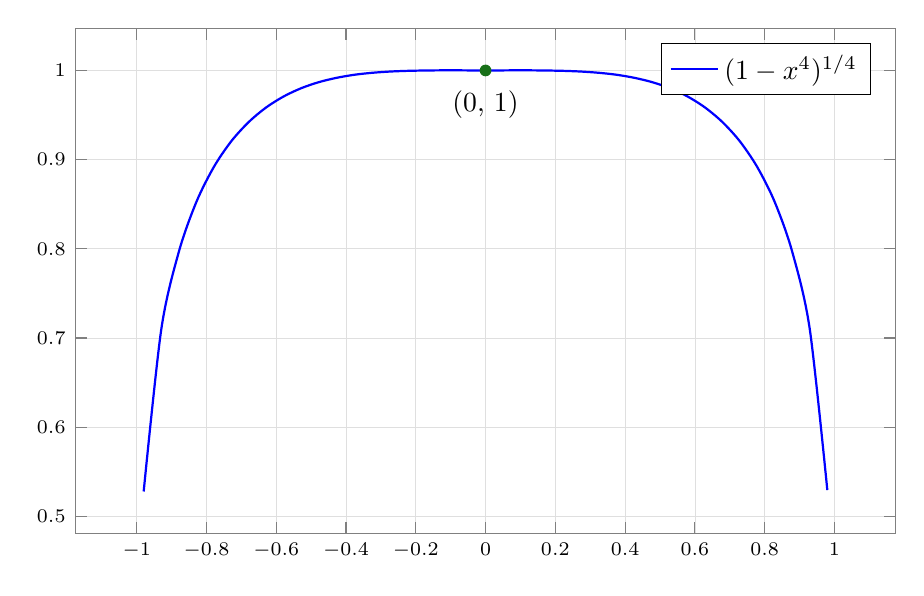
\begin{tikzpicture}
                  \begin{axis}[Ani, grid=both, legend pos = north east]
                      \addplot [GraphSmooth, domain=-5:5]
                      {(1 - x^(4))^(1/4)};
                      \node[GraphNode, y_h, label={270:{(0, 1)}}]
                      at (axis cs:0,1) {};
                      \addlegendentry{$(1 - x^{4})^{1/4}$}
                  \end{axis}
              \end{tikzpicture}
          \end{figure}
          Checking by differentiation and substitution,
          \begin{align}
              4y^{3}\ \dl y     & = -4x^{3} dx &
              y^{3}\ y' + x^{3} & = 0
          \end{align}


    \item Separating variables,

          \begin{align}
              \int \cos ^{2}y\ \dl y                        & = \int \ \dl x &
              \int \frac{1}{2} + \frac{\cos (2y)}{2}\ \dl y & = \int \ \dl x   \\
              \frac{y}{2} + \frac{\sin (2y)}{4}             & =  x + c
          \end{align}
          \begin{figure}[H]
              \centering
              \begin{tikzpicture}
                  \begin{axis}[PiStyleY, Ani, grid=both, legend pos = north west,
                          trig format plots = rad]
                      \addplot [GraphSmooth, y_h, domain=-pi:pi]
                      ({x/2 + sin(2*x)/4}, {x});
                      \node[GraphNode, label={270:{(0, 0)}}]
                      at (axis cs:0,0) {};
                      \addlegendentry{$x = y/2 + \sin(2y)/4$}
                  \end{axis}
              \end{tikzpicture}
          \end{figure}
          Checking by differentiation and substitution,
          \begin{align}
              dx & = \frac{(1 + \cos(2y))\ dy}{2} &
              y' & = \sec ^{2}y
          \end{align}


    \item Separating variables, with $u = \sin(2 \pi x)$

          \begin{align}
              \int \frac{1}{y} \ \dl y & = \pi \int \frac{\cos(2 \pi x)}
              {\sin (2 \pi x)}\ \dl x  &
              \dl u                    & = 2 \pi \cos(2 \pi x)\ \dl x      \\
              \int \frac{2}{y}\ \dl y  & = \int \frac{1}{u}\ \dl u       &
              2 \ln |y|                & =  \ln |u| + b                    \\
              y^{2}                    & = c\ |\sin(2 \pi x)|
          \end{align}
          \begin{figure}[H]
              \centering
              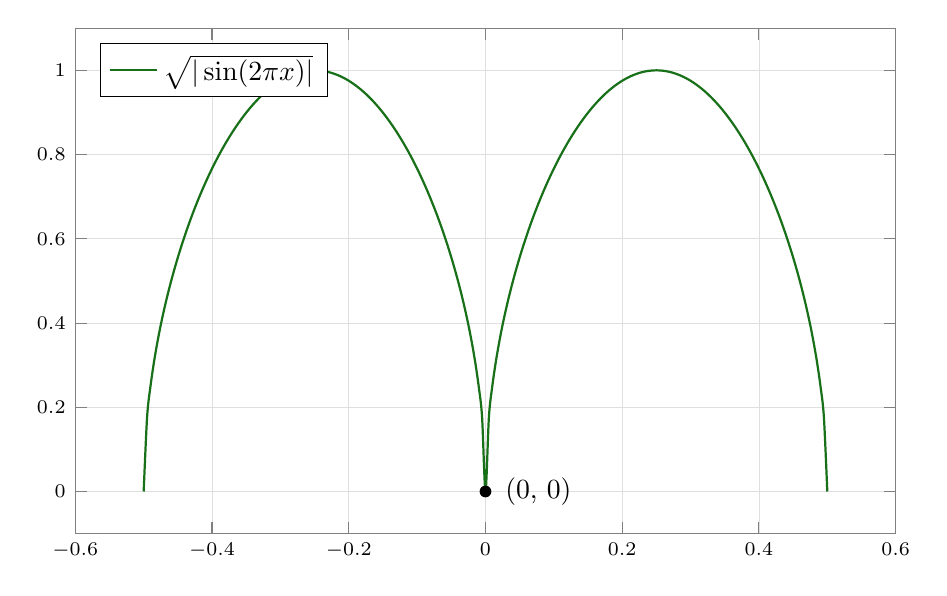
\begin{tikzpicture}
                  \begin{axis}[Ani, grid=both, legend pos = north west,
                          trig format plots = rad]
                      \addplot [GraphSmooth, y_h, domain=-0.5:0.5, samples = 201]
                      {(abs(sin(2 * pi * x)))^0.5};
                      \node[GraphNode, label={0:{(0, 0)}}]
                      at (axis cs:0,0) {};
                      \addlegendentry{$\sqrt{ |\sin(2 \pi x)| }$}
                  \end{axis}
              \end{tikzpicture}
          \end{figure}
          Checking by differentiation and substitution,
          \begin{align}
              y' & = \begin{dcases}
                         \frac{\pi \ \cos(2 \pi x)}{\sqrt{\sin (2 \pi x)}}
                         =  \frac{\pi y \ \cos(2 \pi x)}{\sin (2 \pi x)}   &
                         \mathrm{for} \quad x >= 0                           \\
                         \frac{-\pi \ \cos(-2 \pi x)}{\sqrt{\sin (-2 \pi x)}}
                         =  \frac{-\pi y \ \cos(2 \pi x)}{\sin (-2 \pi x)} &
                         \mathrm{for} \quad  x < 0                           \\
                     \end{dcases}
          \end{align}


    \item Separating variables,

          \begin{align}
              \int y\ \dl y   & = -36 \int x\ \dl x &
              y^{2} + 36x^{2} & =  c
          \end{align}
          \begin{figure}[H]
              \centering
              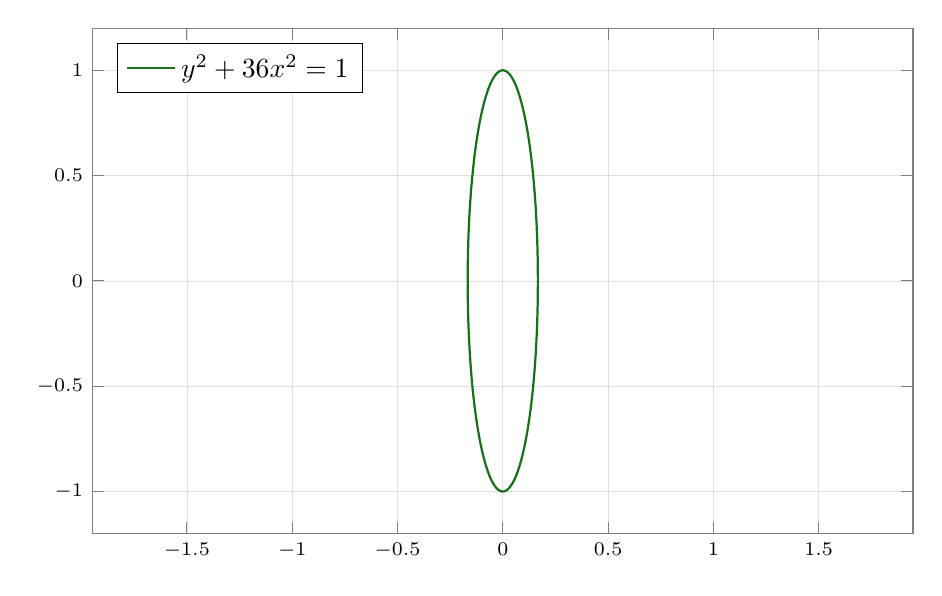
\begin{tikzpicture}
                  \begin{axis}[Ani, grid=both, legend pos = north west,                           xticklabel style={/pgf/number format/fixed}, axis equal]
                      \addplot [GraphSmooth, y_h, domain=-pi:pi, variable=\t]
                      ({sin(t)/6}, {cos(t)});
                      \addlegendentry{$y^{2} + 36x^{2} = 1$}
                  \end{axis}
              \end{tikzpicture}
          \end{figure}
          Checking by differentiation and substitution,
          \begin{align}
              2y\ y'      & = -72x\ \dl x &
              y\ y' + 36x & = 0
          \end{align}


    \item Separating variables,

          \begin{align}
              \int \frac{1}{y^2}\ \dl y & = \int \exp(2x - 1)\ \dl x   &
              \frac{-1}{y}              & = \frac{\exp(2x - 1)}{2} + b   \\
              y                         & =  \frac{-2}{c + e^{(2x-1)}}
          \end{align}
          \begin{figure}[H]
              \centering
              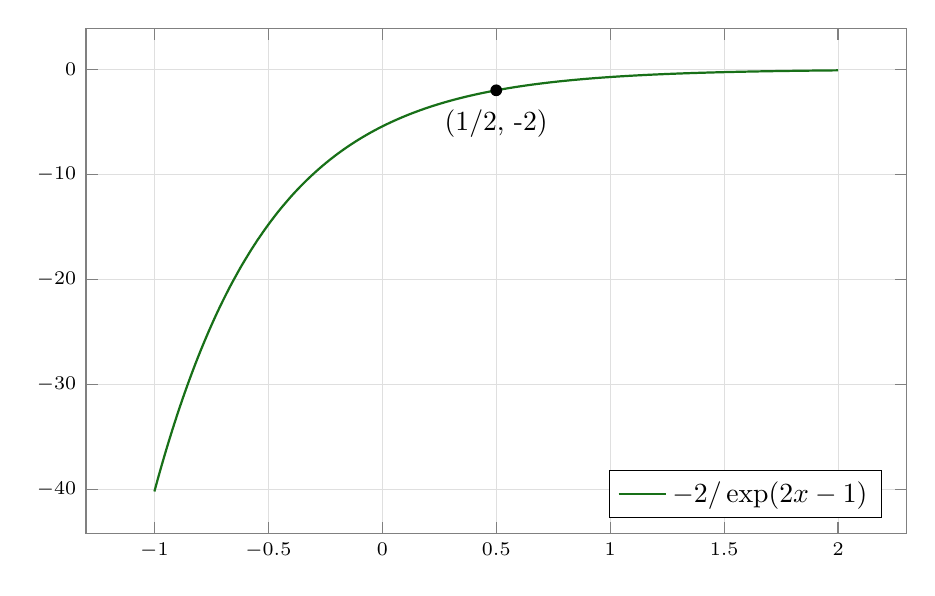
\begin{tikzpicture}
                  \begin{axis}[Ani, grid=both, legend pos = south east]
                      \addplot [GraphSmooth, y_h, domain=-1:2]
                      {-2 * (e^(2*x - 1))^(-1)};
                      \node[GraphNode, label={270:{(1/2, -2)}}]
                      at (axis cs:1/2,-2) {};
                      \addlegendentry{$-2/\exp(2x-1)$}
                  \end{axis}
              \end{tikzpicture}
          \end{figure}
          Checking by differentiation and substitution,
          \begin{align}
              y' & = \frac{4\ e^{(2x-1)}}{(c + e^{(2x-1)})^{2}} &
              y' & = y^{2}\ e^{(2x-1)}
          \end{align}


    \item Using $u = y/x$.

          \begin{align}
              y'                            & = u + \frac{2 y^{2}}{u^{2}} \sin^{2} u \\
              x\ du + u\ \dl x              & = (u + x^{2} \sin ^{2} u )\ \dl x      \\
              \int \frac{1}{\sin ^{2}u}\ du & = \int x\ \dl x                        \\
              - \cot u                      & = \frac{x^{2}}{2} + b                  \\
              y                             & = x\ \arctan \left(\frac{2}{c - x^{2}}
              \right)
          \end{align}
          \begin{figure}[H]
              \centering
              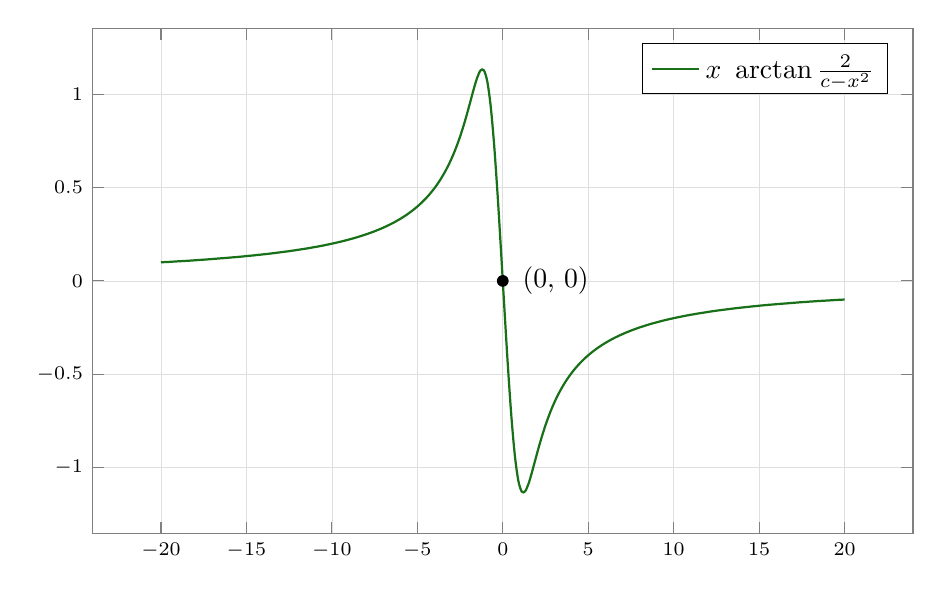
\begin{tikzpicture}
                  \begin{axis}[Ani, grid=both, legend pos = north east]
                      \addplot [GraphSmooth, y_h, domain=-20:20]
                      {x * atan(2 / (-1*x*x))};
                      \node[GraphNode, label={0:{(0, 0)}}]
                      at (axis cs:0,0) {};
                      \addlegendentry{$x\ \arctan \frac{2}{c-x^{2}}$}
                  \end{axis}
              \end{tikzpicture}
          \end{figure}
          Checking by differentiation and substitution,
          \begin{align}
              y' & = \arctan \left(\frac{2}{c - x^{2}}\right) +
              \frac{x\ (c - x^{2})^{2}}{4 + (c - x^{2})^{2}}
              \times \frac{4x}{(c - x^{2})^{2}}                         \\
              y' & = \frac{y}{x} + x^{2}\ \frac{4}{4 + (c - x^{2})^{2}} \\
              y' & = \frac{y}{x} + x^{2} \ \sin ^{2}
              \left[\arctan\left(\frac{2}{c - x^{2}}\right)\right] = \frac{y}{x}
              + x^{2}\ \sin ^{2} \left(\frac{y}{x}\right)
          \end{align}


    \item Using $u = y + 4x$.

          \begin{align}
              u' - 4                                       & = u^{2}                &
              \int \frac{1}{4 + u^{2}}\ du                 & = \int \ \dl x           \\
              \frac{1}{2} \arctan \left(\frac{u}{2}\right) & = x + b                &
              y                                            & = 2 \tan (2x + c) - 4x
          \end{align}
          \begin{figure}[H]
              \centering
              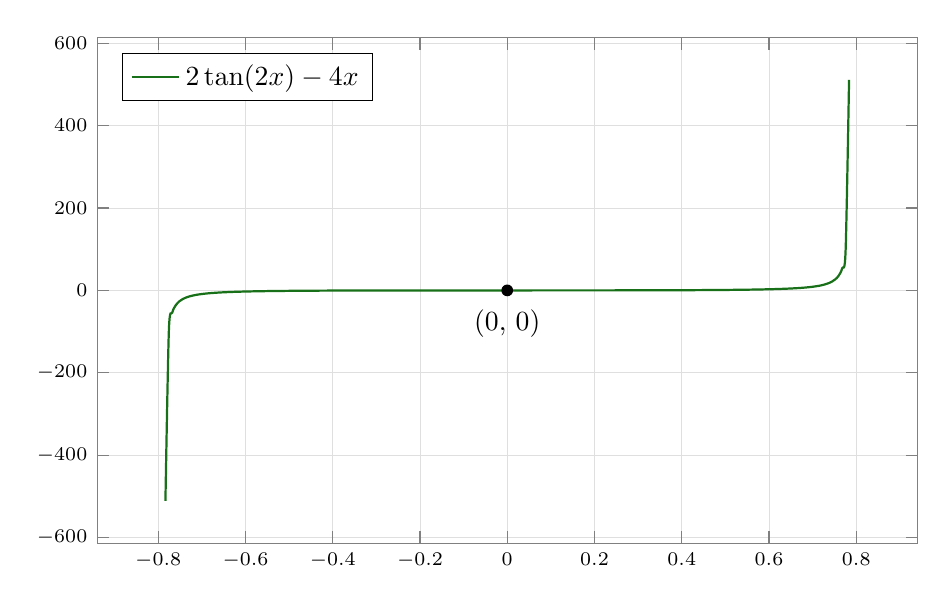
\begin{tikzpicture}
                  \begin{axis}[Ani, grid=both, legend pos = north west,
                          trig format plots = rad]
                      \addplot [GraphSmooth, y_h, domain=-pi/4.01:pi/4.01,
                          samples = 201]
                      {2 * tan(2*x) - 4*x};
                      \node[GraphNode, label={270:{(0, 0)}}]
                      at (axis cs:0,0) {};
                      \addlegendentry{$2 \tan (2x) - 4x$}
                  \end{axis}
              \end{tikzpicture}
          \end{figure}
          Checking by differentiation and substitution,
          \begin{align}
              y' & = -4 + \frac{4}{\cos ^{2}(2x + c)}              \\
              y' & = 4 \frac{\sin ^{2}(2x + c)}{\cos ^{2}(2x + c)}
              = (2 \tan (2x+c))^{2}                                \\
              y' & = (y + 4x)^{2}
          \end{align}


    \item Using $u = y/x$.

          \begin{align}
              y'                       & = xu^{2} + u = u + xu'                  &
              \int \frac{1}{u^{2}}\ du & = \int \ \dl x                            \\
              \frac{-1}{u}             & = x + b = \frac{-x}{y}                  &
              y                        & = \frac{-x}{x + c} = \frac{-1}{1 + c/x}
          \end{align}
          \begin{figure}[H]
              \centering
              \begin{tikzpicture}
                  \begin{axis}[Ani, grid=both, legend pos = north west,
                          trig format plots = rad, restrict y to domain = -100:100]
                      \addplot [GraphSmooth, y_h, domain=-2.5:0.5, samples = 200,
                      ]
                      {-x / (x + 1)};
                      \node[GraphNode, label={270:{(0, 0)}}]
                      at (axis cs:0,0) {};
                      \addlegendentry{$-x / (x + 1)$}
                  \end{axis}
              \end{tikzpicture}
          \end{figure}
          Checking by differentiation and substitution,

          \begin{align}
              xy'       & = \frac{-cx}{(x+c)^{2}}                 &
              y + y^{2} & = \frac{-x^{2} + x^{2} - cx}{(x+c)^{2}}   \\
              xy'       & = y + y^{2}
          \end{align}


    \item Using $u = y/x$.

          \begin{align}
              y'       & = 1 + u = u + xu'         &
              \int\ du & = \int \frac{1}{x}\ \dl x   \\
              u        & = \ln |x| + b             &
              y        & = x \ln |x| + cx
          \end{align}
          \begin{figure}[H]
              \centering
              \begin{tikzpicture}
                  \begin{axis}[Ani, grid=both, legend pos = north west,
                          trig format plots = rad]
                      \addplot [GraphSmooth, y_h, domain=-1:1, samples = 100
                      ]
                      {x * ln(abs(x)) + x};
                      \node[GraphNode, label={45:{(0, 0)}}]
                      at (axis cs:0,0) {};
                      \addlegendentry{$x\ (\ln|x| + 1)$}
                  \end{axis}
              \end{tikzpicture}
          \end{figure}
          Checking by differentiation and substitution,
          \begin{align}
              xy'   & = xc + x\ln |x| + x &
              x + y & = xy'
          \end{align}


    \item Given IC is $y(4) = 6$

          \begin{align}
              y'                        & = \frac{-y}{x}             &
              \int \frac{-1}{y} \ \dl y & = \int \frac{1}{x} \ \dl x   \\
              \ln |y|                   & = -\ln |x|  - b            &
              |y|                       & = \frac{c}{ |x| }            \\
              c                         & = 24                       &
              \implies y                & = \frac{24}{x}
          \end{align}
          \begin{figure}[H]
              \centering
              \begin{tikzpicture}
                  \begin{axis}[Ani, grid=both, legend pos = north west,
                          trig format plots = rad]
                      \addplot [GraphSmooth, y_h, domain=-8:8, samples = 200,
                          restrict y to domain = -100:100]
                      {24/x};
                      \node[GraphNode, label={45:{(4, 6)}}]
                      at (axis cs:4, 6) {};
                      \addlegendentry{$24 / x$}
                      \addplot [GraphSmooth, y_p, domain=-8:8, samples = 200,
                          restrict y to domain = -100:100]
                      {-24/x};
                      \node[GraphNode, label={45:{(4, 6)}}]
                      at (axis cs:4, 6) {};
                      \addlegendentry{$-24 / x$}
                  \end{axis}
              \end{tikzpicture}
          \end{figure}
          Checking by differentiation and substitution,
          \begin{align}
              y            & = \frac{24}{x}      &
              y'           & = \frac{-24}{x^2}     \\
              \frac{-y}{x} & = \frac{-24}{x^{2}}
          \end{align}


    \item Given IC is $y(1) = 0$

          \begin{align}
              y'                                 & = 1 + 4y^{2}             &
              \int \frac{1}{y^{2} + 1/4} \ \dl y & = \int 4 \ \dl x           \\
              2 \arctan(2y)                      & = 4x + c                 &
              c                                  & = -4                       \\
              y                                  & =\frac{\tan (2x - 2)}{2}
          \end{align}
          \begin{figure}[H]
              \centering
              \begin{tikzpicture}
                  \begin{axis}[Ani, grid=both, legend pos = north west,
                          trig format plots = rad, restrict y to domain = -100:100]
                      \addplot [GraphSmooth, y_h, domain=1 - pi/4:1 + pi/4,
                          restrict y to domain = -100:100]
                      {0.5 * tan(2*x - 2)};
                      \node[GraphNode, label={45:{(1, 0)}}]
                      at (axis cs:1, 0) {};
                      \addlegendentry{$24 / x$}
                  \end{axis}
              \end{tikzpicture}
          \end{figure}
          Checking by differentiation and substitution,
          \begin{align}
              1 + 4y^{2} & = 1 + \tan ^{2} (2x - 2) = \sec ^{2} (2x - 2) \\
              y'         & = \sec^{2} (2x - 2)
          \end{align}


    \item Given IC is $y(0) = \pi / 2$

          \begin{align}
              \int \frac{1}{\sin ^{2}y} \ \dl y
                      & = \int \frac{1}{\cosh ^{2}x} \ \dl x          \\
              -\cot y & = \tanh x + c                                 \\
              y       & = \arctan \left(\frac{-1}{\tanh x + c}\right) \\
              c       & = 0                                           \\
              y       & = \arctan\left(\frac{-1}{\tanh x}\right)
          \end{align}
          Checking by differentiation and substitution,
          \begin{align}
              y'               & = \frac{\tanh ^{2}x}{1 + \tanh ^{2}x} \times
              \frac{1}{\tanh ^{2}x} \times \frac{1}{\cosh ^{2}x}                  \\
              y' \cosh ^{2}(x) & = \frac{1}{1 + \tanh ^{2}x}                      \\
                               & = \frac{(-1/\tanh x)^{2}}{1 + (-1/ \tanh x)^{2}}
              = \sin ^{2} \left[\arctan\left(\frac{-1}{\tanh x}\right)\right]     \\
                               & = \sin ^{2} y
          \end{align}


    \item Given IC is $r(0) = r_{0}$

          \begin{align}
              \dl r                    & = -2tr \ \dl t        &
              \int \frac{1}{r} \ \dl r & = \int -2t \ \dl t      \\
              \ln |r|                  & = -t^{2} + b          &
              |r|                      & = c \exp (-t^{2})       \\
              c                        & = r_{0}               &
              r                        & = r_{0} \exp (-t^{2})
          \end{align}
          \begin{figure}[H]
              \centering
              \begin{tikzpicture}
                  \begin{axis}[Ani, grid=both, legend pos = north east,
                          trig format plots = rad, ]
                      \addplot [GraphSmooth, y_h, domain=0:3,
                      ]
                      {e^(-x*x)};
                      \node[GraphNode, label={270:{(0, $r_{0}$)}}]
                      at (axis cs:0, 1) {};
                      \addlegendentry{$r_{0} \exp(-t^{2})$}
                  \end{axis}
              \end{tikzpicture}
          \end{figure}
          Checking by differentiation and substitution,
          \begin{align}
              r'   & = c \exp (-t^{2}) \times (-2t)  &
              -2tr & = (-2t) \times c \exp (-2t^{2})
          \end{align}


    \item Given IC is $y(2) = 3$

          \begin{align}
              \int y \ \dl y  & = \int -4x \ \dl x &
              \frac{y^{2}}{2} & = -2x^{2} + b        \\
              y^{2} + 4x^{2}  & = c                &
              c               & = 25
          \end{align}
          \begin{figure}[H]
              \centering
              \begin{tikzpicture}
                  \begin{axis}[Ani, grid=both, legend pos = north west, axis equal,
                          trig format plots = rad,]
                      \addplot [GraphSmooth, y_h, domain=-pi:pi, variable = \t
                      ]
                      ({2.5 * sin(t)}, {5*cos(t)});
                      \node[GraphNode, label={45:{(2, 3)}}]
                      at (axis cs:2, 3) {};
                      \addlegendentry{$y^{2} + 4x^{2} = 25$};
                  \end{axis}
              \end{tikzpicture}
          \end{figure}
          Checking by differentiation and substitution,
          \begin{align}
              2yy' + 8x & = 0             &
              y'        & = \frac{-4x}{y}
          \end{align}


    \item Given IC is $y(0) = 2$, and substituting $u = x+y-2$

          \begin{align}
              y'                             & = u^{2}  = u' - 1      \\
              \int\ \frac{1}{1+u^{2}}\ \dl u & = \int\ \dl x          \\
              \arctan (u)                    & = x + c                \\
              y                              & = 2 - x + \tan (x + c) \\
              c                              & = 0
          \end{align}
          \begin{figure}[H]
              \centering
              \begin{tikzpicture}
                  \begin{axis}[Ani, grid=both, legend pos = north east]
                      \addplot [GraphSmooth, y_h, domain=-2*pi:2*pi, samples = 400,
                          restrict y to domain = -25:25]
                      {2 - x + tan(x)};
                      \node[GraphNode, label={45:{(0, 2)}}]
                      at (axis cs:0, 2) {};
                      \addlegendentry{$2 - x + \tan(x)$};
                  \end{axis}
              \end{tikzpicture}
          \end{figure}
          Checking by differentiation and substitution,
          \begin{align}
              y'             & = -1 + \sec ^{2} (x + c) = \tan ^{2} ( x + c) \\
              (x + y -2)^{2} & = \tan ^{2} (x + c)
          \end{align}


    \item Given IC is $y(1) = 0$, and substituting $u = y/x$

          \begin{align}
              y'                     & = u + 3x^{3} \cos ^{2} u = u + xu' \\
              \int\ \sec^{2}u\ \dl u & = \int\ 3x^{2}\ \dl x              \\
              \tan u                 & = x^{3} + c                        \\
              y                      & = x\ \arctan (x^{3} + c)           \\
              c                      & = -1
          \end{align}
          \begin{figure}[H]
              \centering
              \begin{tikzpicture}
                  \begin{axis}[Ani, grid=both, legend pos = north east,
                          trig format plots = rad]
                      \addplot [GraphSmooth, y_h, domain=-4:4, samples = 200
                      ]
                      {x * atan(x^3 - 1)};
                      \node[GraphNode, label={0:{(1, 0)}}]
                      at (axis cs:1, 0) {};
                      \addlegendentry{$x\ \arctan(x^{3} + c)$};
                  \end{axis}
              \end{tikzpicture}
          \end{figure}
          Checking by differentiation and substitution,
          \begin{align}
              y'      & = \arctan (x^{3} + c) + \frac{3x^{3}}
              {1 + (x^{3} + c)^{2}}                                  \\
              xy' - y & = \frac{3x^{4}}{1 + (x^{3} + c)^{2}}         \\
              3x^{4} \times \cos ^{2}(y/x)
                      & = 3x^{4} \times \frac{1}{1 + (x^{3} +c)^{2}}
          \end{align}


    \item Introducing limits into the equation

          \begin{align}
              \int\ g(y)\ \dl y                  & = \int\ f(x)\ \dl x + c             \\
              y(x_{0})                           & = y_{0}                             \\
              \int_{x_{0}}^{x}\ f(x) \ \dl x + c & = \int_{x_{0}}^{x} \ g(y) y'\ \dl x \\
                                                 & = \int_{y(x_{0})}^{y(x)} \ g(y)
              \ \dl y                                                                  \\
                                                 & = \int_{y_{0}}^{y} \ g(y)\ dy
          \end{align}


    \item Given IC is $y(t = 0) = y_{0}$ where $ t $ is the time in weeks, and $ y $
          is the number of bacteria.

          \begin{align}
              \diff yt       & = ky                  &
              \ln        |y| & = kt + b                \\
              y              & = c e^{kt} \qquad y>0 &
              c              & = y_{0}
          \end{align}
          \begin{figure}[H]
              \centering
              \begin{tikzpicture}
                  \begin{axis}[Ani, grid=both, legend pos = north west,
                          xlabel = time ($ t $),
                          ylabel = bacteria count ratio ($ y / y_{0} $)]
                      \addplot [GraphSmooth, y_h, domain=0:5
                      ]
                      {e^(x*ln(2))};
                      \node[GraphNode, label={90:{(0, 1)}}] at (axis cs:0, 1) {};
                      \node[GraphNode, label={90:{(2, 4)}}] at (axis cs:2, 4) {};
                      \node[GraphNode, label={-45:{(4, 16)}}] at (axis cs:4, 16) {};
                      \addlegendentry{$y = y_{0}\   e^{t \ln 2 } = y_{0}2^{t}$};
                  \end{axis}
              \end{tikzpicture}
          \end{figure}
          Inserting into ODE solution,
          \begin{align}
              y(t = 2) & = 2y_{0}   &
              y(t = 4) & = 16 y_{0}
          \end{align}


    \item Given IC is $y(t = 0) = y_{0}$ where $ t $ is the time in weeks, and $ y $
          is the number of bacteria, $ b $ is the birth rate and $ k $ is the death rate

          \begin{align}
              \diff yt       & = by - ky                 &
              \ln        |y| & = (b-k)t + c                \\
              y              & = c e^{(b-k)t} \qquad y>0 &
              c              & = y_{0}
          \end{align}
          \begin{figure}[H]
              \centering
              \begin{tikzpicture}
                  \begin{axis}[Ani, grid=both, legend pos = north west,
                          xlabel = time ($ t $),
                          ylabel = bacteria count ratio ($ y / y_{0} $)]
                      \addplot [GraphSmooth, y_h, domain=0:2] {e^(x)};
                      \addplot [GraphSmooth, y_p, domain=0:2] {e^(-x)};
                      \addplot [GraphSmooth, y_t, domain=0:2] {e^(0)};
                      \node[GraphNode, label={90:{(0, 1)}}] at (axis cs:0, 1) {};
                      \addlegendentry{$y = y_{0}\ e^{t}$};
                      \addlegendentry{$y = y_{0}\ e^{-t}$};
                      \addlegendentry{$y = y_{0}$};
                  \end{axis}
              \end{tikzpicture}
          \end{figure}
          Interpreting the results,
          \begin{align}
              \lim_{t \to \infty}\ y & =
              \begin{cases}
                  \infty & \quad \mathrm{if} \quad b>k \\
                  0      & \quad \mathrm{if} \quad b<k \\
                  y_{0}  & \quad \mathrm{if} \quad b=k
              \end{cases}
          \end{align}


    \item Given IC is $y(t = 0) = y_{0}$ where $ t $ is the time in years, and $ y $
          is the quantity of C-14.
          Half life of C-14 is $ T_{1/2} = 5715 $ years.

          \begin{align}
              \diff yt       & = - ky                  &
              \ln        |y| & = -kt + c                 \\
              y              & = c e^{-kt} \qquad y>0  &
              c              & = y_{0}                   \\
              k              & = \frac{\ln 2}{T_{1/2}}
          \end{align}

          \begin{figure}[H]
              \centering
              \begin{tikzpicture}
                  \begin{axis}[Ani, grid=both, legend pos = north east,
                          xlabel = time in years ($ t $),
                          ylabel = C-14 ratio ($ y / y_{0} $)]
                      \addplot [GraphSmooth, y_h, domain=0:5800] {e^(-x * (ln(2)/5715))};
                      \node[GraphNode, label={0:{(0, 1)}}] at (axis cs:0, 1) {};
                      \node[GraphNode, label={45:{(3000, 0.695)}}]
                      at (axis cs:3000, 0.695) {};
                      \addlegendentry{$y = y_{0}\ e^{-1.213 \times 10^{-4}\ t}$};
                  \end{axis}
              \end{tikzpicture}
          \end{figure}
          After 3000 years the C-14 content is $ 69.5 \% $ of $ y_{0} $.

    \item For the particle, let $ v_{0} $ be initial velocity, $ v (t) $ be the
          velocity at time $ t $
          in seconds.

          \begin{align}
              \frac{dv}{dt} & = v' = k                                            \\
              v             & = kt + c                                            \\
              c             & = v_{0}                                             \\
              k             & =\frac{v - v_{0}}{t} = \frac{\num{9e3}}{\num{1e-3}}
              = \SI{9e6}{\meter \per \square \second}
          \end{align}
          In order to find the distance traveled $ s $ in time $ t $,
          \begin{align}
              v = \diff st & = kt + v_{0}                    &
              s            & = \frac{kt^{2}}{2} + v_{0}t + b   \\
              b            & = 0                             &
              s            & = 4.5 + 1 = \SI{5.5}{\meter}
          \end{align}


    \item At constant temperature, pressure $ p $ and volume $ V $ are related by,

          \begin{align}
              \frac{dV}{dp} = \frac{-V}{p}                           \\
              \int\ \frac{-1}{V}\ dV       & = \int\ \frac{1}{p}\ dp \\
              \ln \left(\frac{1}{V}\right) & = \ln p + b             \\
              Vp                           & = c
          \end{align}


    \item Standard mixing problem with brine $ y $ in lb and time $ t $ in minutes

          \begin{align}
              \diff yt                 & = 0 - \frac{2y}{400}                      \\
              \int\ \frac{1}{y}\ \dl y & = \frac{-1}{200} \int\ \dl t              \\
              y                        & = c e^{-t/200}                            \\
              y(t = 0)                 & = 100                                   &
              c                        & = 100                                     \\
              y(t = 60)                & = 100 \times \exp \left(\frac{-60}{200}
              \right) = \SI{74.08}{lb}
          \end{align}

          After 1 hour, 74.08 lb of salt remains in the tank

    \item Newton's law of cooling problem, with temperature $ y $ in celsius and time
          $ t $ in minutes

          \begin{align}
              \diff yt                         & = k(y - y_{A})                   \\
              \int\ \frac{1}{y - y_{A}}\ \dl y & = k \int\ \dl t                  \\
              y                                & = y_{A} + c e^{kt}               \\
              y_{A}                            & = 22                 & c & = -17 \\
              y(t = 1)                         & = 22 - 17 e^{k} = 12 & k & = \ln
              \left(\frac{10}{17}\right)                                          \\
              21.9                             & = 22 - 17e^{kt}      & t & =9.68
          \end{align}

          For the temperature to be \SI{21.9}{\celsius}, the time taken is
          $ \SI{9.68}{\minute} $

    \item Gompertz growth model for tumours, with time $ t $ and mass of tumour $ y $,

          \begin{align}
              \diff yt            & = -Ay\ln y                          &
              A                   & >0                                    \\
              y'                  & = 0                                 &
              \implies y          & = 0 \qquad \mathrm{or} \qquad y = 1   \\
              y''                 & = -A(1 + \ln y)                       \\
              \implies y''(y = 0) & >0                                  &
                                  & y''(y = 1)< 0
          \end{align}
          $ y = 0 $ is the unstable equilibrium solution of no tumour. $ y = 1 $
          is the stable equilibrium solution. On solving the ODE explicitly,
          \begin{align}
              \diff yt                      & = -Ay \ln y         \\
              \int\ \frac{1}{y\ln y}\ \dl y & = -A \int\ \dl t    \\
              u                             & = \ln y           &
              du                            & = \frac{\dl y}{y}   \\
              \int\ \frac{\dl u}{u}         & = -At + b         &
              \ln u                         & = -At + b           \\
              \ln y                         & = ce^{-At}        &
              y                             & = \exp(ce^{-At})    \\
              y(t = 0)                      & = e^{c}           &
              y_{0} > 1                     & \implies c > 0
          \end{align}

          \begin{figure}[H]
              \centering
              \begin{tikzpicture}
                  \def\U{1}
                  \def\V{-y*ln(y)}
                  \def\LEN{sqrt(\U * \U + \V * \V)}
                  \begin{axis}[
                          legend pos = outer north east,
                          width = 8cm,
                          height = 8cm,
                          Ani,
                          axis equal,
                          view     = {0}{90}, % for a view 'from above'
                      ]
                      \addplot3 [
                          forget plot,
                          domain = 0:5,
                          color = gray!50,
                          point meta = {\LEN},
                          quiver={u={(\U) / \LEN},
                                  v={(\V) / \LEN},
                                  scale arrows = 0.2,},
                          -stealth,
                          samples=20,
                      ] (x, y, 0);
                      \addplot [thick, GraphSmooth, y_h, domain=0:5]
                      {e^(e^(-x))};
                      \addlegendentry{$ c = 1 $ and $A = 1$};
                      \addplot [thick, GraphSmooth, y_p, domain=0:5]
                      {e^(-10*e^(-x))};
                      \addlegendentry{$ c = -10 $ and $ A = 1 $};
                  \end{axis}
              \end{tikzpicture}
          \end{figure}
          Solutions with $ y_{0} > 1 $ decay to the steady state
          solution $ y = 1 $, whereas $ y_{0} < 1$ increases sigmoidally to the same
          stable equilibrium value.

    \item Let $ y $ be the moisture content and $ t $ be time in minutes.

          \begin{align}
              \diff yt    & = -ky                                                 \\
              y           & = ce^{-kt}                 & c & = y_{0}              \\
              y(t = 10)   & = y_{0} e^{-10k} = y_{0}/2 & k & = \frac{\ln 2}{10}   \\
              y_{0} / 100 & = y_{0} e^{-kt}            & t & = \SI{66.4}{\minute}
          \end{align}


    \item It will take between 60 and 70 minutes since $ 64 < 100 < 128 $ and
          thus $ 2^{6} < 2^{t*} < 2^{7} $. $ t* = 6.64$.
          \stepcounter{equation}

    \item Using Newton's Law of cooling, consider the temperature $ y $ in
          Fahrenheit and time $ t $ in minutes

          \begin{align}
              \diff yt                         & = k(y - y_{A})           \\
              \int\ \frac{1}{y - y_{A}}\ \dl y & = k \int\ \dl t          \\
              y                                & = y_{A} + c e^{kt}       \\
              y(t = 30)                        & = y_{A} + ce^{30k}     &
              y(t = 40)                        & =y_{A} + ce^{40k}        \\
              190 - 110 = 80                   & = c(e^{30k} - e^{40k})
          \end{align}


          Since Newton's law of cooling specifies that the rate of cooling slows down
          with time, $ y_{20} - y_{30} > y_{30} - y_{40}$.
          This means $ y_{20} > 270$ F. Since this is above boiling point of water,
          Jack can only have been inside the bar for about 6 minutes at
          most.

    \item In the first powered stage, the distance travelled by the rocket is,

          \begin{align}
              y''       & = 7t                                               \\
              y         & = \frac{7t^{3}}{6} + bt + c                        \\
              y(t = 0)  & = c = 0                     & y'(t=0)    & = b = 0 \\
              y(t = 10) & = \frac{7000}{6}            & y'(t = 10) & = 350
          \end{align}
          In the next stage, under the influence of only gravity
          ($ g = \SI{10}{\meter\per\second\squared} $), the distance traveled is,
          \begin{align}
              y_{f} & = \frac{0^{2} - 350^{2}}{-2g} = \SI{6125}{\meter}
          \end{align}


          The maximum height reached by the rocket is thus, $ \SI{7291.7}{\meter} $

    \item Non-vertical straight line through the origin is of the form $ y = mx $
          for finite $ m $.
          \begin{figure}[H]
              \centering
              \begin{tikzpicture}
                  \def\U{x}
                  \def\V{-y}
                  \def\LEN{sqrt(\U * \U + \V * \V)}
                  \begin{axis}[
                          legend pos = outer north east,
                          width = 8cm,
                          height = 8cm,
                          Ani,
                          axis equal,
                          view     = {0}{90}, % for a view 'from above'
                      ]
                      \addplot3 [domain = -4:4,
                          color = gray!50,
                          point meta = {\LEN},
                          quiver={u={(\U) / \LEN},
                                  v={(\V) / \LEN},
                                  scale arrows = 0.25,},
                          -stealth,
                          samples=16,
                      ] (x, y, 0);
                      \addplot [GraphSmooth, domain=-4:4,
                          color = y_t!50,
                          restrict y to domain = -4:4] {1/x};
                      \addplot [GraphSmooth, domain=-4:4,
                          color = y_h!50,
                          restrict y to domain = -4:4] {4/x};
                      \addplot [GraphSmooth, domain=-4:4,
                          color = y_p!50] {x};
                      \addlegendentry{$ y' = -y/x $};
                      \addlegendentry{$ y = 1/x $};
                      \addlegendentry{$ y = 4/x $};
                      \addlegendentry{$ y = x $}
                      \draw[y_p,->, thick] (axis cs:1,1) -- (axis cs:2,2);
                      \draw[y_t,->, thick] (axis cs:1,1) -- (axis cs:2,0);
                      \draw[y_p,->, thick] (axis cs:2,2) -- (axis cs:3,3);
                      \draw[y_h,->, thick] (axis cs:2,2) -- (axis cs:3,1);
                  \end{axis}
              \end{tikzpicture}
          \end{figure}

          Consider the set of solutions to the ODE $ y' = g(y/x) $ intersecting
          the line $ y = mx $. $ y' = g(m) $ by definition, which means that the tangents
          to the family of solutions to the ODE are all parallel and aligned in the
          direction $ g(m) $. This means that the line $ y = mx $ intersects all of
          the solutions of the ODE at the angle between the directions $ m $ and
          $ g(m) $.

    \item Resolving the gravitational force on the block into two components along and
          perpendicular to the inclined plane,

          \begin{align}
              N  & = mg\ \cos \alpha                  &
                 & \text{perpendicular to plane}        \\
              ma & = mg\ \sin \alpha - f              &
                 & \text{along plane}                   \\
              f  & = \mu N = \mu mg\ \cos \alpha      &
                 & \text{kinetic friction}              \\
              a  & = g(\sin \alpha - \mu \cos \alpha)
                 &                                    &
              = 10 \left(\frac{1}{2}
              - \frac{0.2\sqrt{3}}{2}\right)
          \end{align}
          Now, given the initial velocity $ u = \SI{0}{\meter\per\second} $, and the
          distance to slide along the plane $ s = \SI{10}{\meter} $,
          \begin{align}
              v^{2} & = u^{2} + 2as                       \\
                    & = (1 - 0.2 \sqrt{3}) \times 100     \\
              v     & = 10 \times \sqrt{1 - 0.2 \sqrt{3}}
              = \SI{8.08}{\meter\per\second}
          \end{align}


    \item Given force $ S $ and angle $ \phi $,

          \begin{align}
              \Delta S              & = kS\ \Delta \phi         &
              \int\ \frac{1}{S}\ dS & = k \int\ d\phi             \\
              S                     & = ce^{k\phi}              &
              c                     & = S_{0}                     \\
              \phi                  & = \frac{\ln (1000)}{0.15} &
              \phi                  & = 2\pi \times 7.34
          \end{align}

          Thus, 7.5 revolutions of the rope around the bollard is enough to withstand a
          force 1000 times larger on the other end of the rope (because of the nature
          of exponential increase).

    \item For conic sections,
          \begin{enumerate}
              \item For cirlces with center as the origin, the equation is,

                    \begin{align}
                        y^{2} + x^{2} & = r^{2}        &
                        2yy' + 2x     & = 0              \\
                        y'            & = \frac{-x}{y}
                    \end{align}
              \item For the family of parabolas $ xy = c $,
                    \begin{align}
                        xy' + y & = 0            &
                        y'      & = \frac{-y}{x}
                    \end{align}
                    \begin{figure}[H]
                        \centering
                        \begin{tikzpicture}
                            \def\U{x}
                            \def\V{-y}
                            \def\LEN{sqrt(\U * \U + \V * \V)}
                            \begin{axis}[
                                    legend pos = outer north east,
                                    width = 8cm,
                                    height = 8cm,
                                    Ani,
                                    axis equal,
                                    view     = {0}{90}, % for a view 'from above'
                                ]
                                \addplot3 [
                                    forget plot,
                                    domain = -4:4,
                                    color = gray!50,
                                    point meta = {\LEN},
                                    quiver={u={(\U) / \LEN},
                                            v={(\V) / \LEN},
                                            scale arrows = 0.25,},
                                    -stealth,
                                    samples=16,
                                ] (x, y, 0);
                                \addplot [GraphSmooth, domain=-4:4, y_h,
                                    restrict y to domain= -4:4]
                                {1/x};
                                \addlegendentry{$ c = 1 $};
                                \addplot [GraphSmooth, domain=-4:4, y_p,
                                    restrict y to domain= -4:4]
                                {-4/x};
                                \addlegendentry{$ c = -4 $};
                            \end{axis}
                        \end{tikzpicture}
                    \end{figure}
              \item For the family of straight lines passing through the origin,
                    $ y = mx $,
                    \begin{align}
                        y' & = m = \frac{y}{x}
                    \end{align}

              \item The product of the RHS of these two families of curves is,
                    \begin{align}
                        \frac{y}{x} \times \frac{-x}{y} & = -1 &
                        m_{1} \times m_{2}              & = -1
                    \end{align}
                    By definition, the product of slopes being -1 is the condition for
                    the two curves to be orthogonal. This also extends to two families
                    of curves being orthogonal.
                    \begin{figure}[H]
                        \centering
                        \begin{tikzpicture}
                            \def\U{y}
                            \def\V{-x}
                            \def\LEN{sqrt(\U * \U + \V * \V)}
                            \begin{axis}[
                                    legend pos = outer north east,
                                    width = 8cm,
                                    height = 8cm,
                                    Ani,
                                    axis equal,
                                    view     = {0}{90}, % for a view 'from above'
                                ]
                                \addplot3 [
                                    forget plot,
                                    domain = -4:4,
                                    color = gray!50,
                                    point meta = {\LEN},
                                    quiver={u={(\U) / \LEN},
                                            v={(\V) / \LEN},
                                            scale arrows = 0.25,},
                                    -stealth,
                                    samples=16,
                                ] (x, y, 0);
                                \addplot [thick, GraphSmooth, y_h, domain=-pi:pi,
                                    variable = \t]
                                ({cos(t)}, {sin(t)});
                                \addplot [thick, GraphSmooth, y_p, domain=-pi:pi,
                                    variable = \t]
                                ({3 * cos(t)}, {3 * sin(t)});
                                \addplot [thick, GraphSmooth, y_s, domain = -4:4,]
                                {x};
                                \addplot [thick, GraphSmooth, y_t, domain = -4:4]
                                {-x};
                                \addlegendentry{$ x^{2} + y^{2} = 1 $};
                                \addlegendentry{$ x^{2} + y^{2} = 9 $};
                                \addlegendentry{$ y = x $};
                                \addlegendentry{$ y = -x $};
                            \end{axis}
                        \end{tikzpicture}
                    \end{figure}
              \item Does every one-parameter family of curves lead to a first order ODE?
                    \begin{align}
                        f(x, y, c) & = 0                          &
                                   & \text{parameter c}             \\
                        g\left(x, y, \frac{dy}{dx}, c\right)
                                   & = 0                          &
                                   & \text{differentiating wrt }x   \\
                        F\left(x, y, \frac{dy}{dx}\right)
                                   & = 0                          &
                                   & \text{eliminating c from the
                            above two expressions}
                    \end{align}

                    The last step is the definition of a first order ODE.
          \end{enumerate}

    \item \begin{enumerate}
              \item Plotting the direction field for the given ODE,
                    \begin{figure}[H]
                        \centering
                        \begin{tikzpicture}
                            \def\U{1}
                            \def\V{e^(-x^(2))}
                            \def\LEN{sqrt(\U * \U + \V * \V)}
                            \begin{axis}[
                                    legend pos = outer north east,
                                    width = 8cm,
                                    height = 8cm,
                                    Ani,
                                    axis equal,
                                    view     = {0}{90}, % for a view 'from above'
                                ]
                                \addplot3 [
                                    forget plot,
                                    domain = -3:3,
                                    color = gray!50,
                                    point meta = {\LEN},
                                    quiver={u={(\U) / \LEN},
                                            v={(\V) / \LEN},
                                            scale arrows = 0.2,},
                                    -stealth,
                                    samples=16,
                                ] (x, y, 0);
                                \addplot[no marks, color = blue!0!red, thick,
                                    domain = -3:3]
                                gnuplot[id=erf]{erf(x) - 2};
                                \addplot[no marks, color = blue!25!red, thick,
                                    domain = -3:3]
                                gnuplot[id=erf]{erf(x) - 1};
                                \addplot[no marks, color = blue!50!red, thick,
                                    domain = -3:3]
                                gnuplot[id=erf]{erf(x)};
                                \addplot[no marks, color = blue!75!red, thick,
                                    domain = -3:3]
                                gnuplot[id=erf]{erf(x) + 1};
                                \addplot[no marks, color = blue!100!red, thick,
                                    domain = -3:3]
                                gnuplot[id=erf]{erf(x) + 2};
                                \node[GraphNode, label={0:\scriptsize {(0, 0)}},
                                    fill = black] at (axis cs:0, 0) {};
                                \addlegendentry{erf$(x) - 2 $};
                                \addlegendentry{erf$(x) - 1 $};
                                \addlegendentry{erf$(x) $};
                                \addlegendentry{erf$(x) + 1 $};
                                \addlegendentry{erf$(x) + 2 $};
                            \end{axis}
                        \end{tikzpicture}
                    \end{figure}

              \item Using the series expansion of $ y' = e^{-x^{2}} $, and integrating
                    the terms in the expansion individually, an approximate solution to
                    the ODE can be plotted

                    \begin{align}
                        y' = e^{-x^{2}} & = 1 - x^{2} + \frac{x^{4}}{4!}
                        - \frac{x^{6}}{6!} + \dots                       \\
                        y               & = x - \frac{x^{3}}{3}
                        + \frac{x^{5}}{5 \cdot 4!} - \frac{x^{7}}{7 \cdot 6!} + \dots
                    \end{align}

                    \begin{figure}[H]
                        \centering
                        \begin{tikzpicture}
                            \def\U{1}
                            \def\V{e^(-x^(2))}
                            \def\LEN{sqrt(\U * \U + \V * \V)}
                            \begin{axis}[
                                    legend pos = outer north east,
                                    width = 8cm,
                                    height = 8cm,
                                    Ani,
                                    axis equal,
                                    view     = {0}{90}, % for a view 'from above'
                                ]
                                \addplot3 [
                                    forget plot,
                                    domain = -1:1,
                                    color = gray!50,
                                    point meta = {\LEN},
                                    quiver={u={(\U) / \LEN},
                                            v={(\V) / \LEN},
                                            scale arrows = 0.1,},
                                    -stealth,
                                    samples=16,
                                ] (x, y, 0);

                                \addplot[no marks, y_h, thick, domain = -1:1]
                                gnuplot[id=erf]{erf(x)};
                                \addplot[thick, GraphSmooth, y_p, domain = -1:1]
                                {x - x^(3)/3 + x^(5)/factorial(5)
                                    - x^(7)/factorial(7) + x^(9)/factorial(9)};
                                \node[GraphNode, label={0:{(0, 0)}}, fill = black]
                                at (axis cs:0, 0) {};
                                \addlegendentry{erf$(x) $};
                                \addlegendentry{$x - x^{3}/3 + x^{5}/5! - x^{7}/7!
                                        + x^{9}/9!$};

                            \end{axis}
                        \end{tikzpicture}
                    \end{figure}

              \item TBC.
          \end{enumerate}

    \item Torricelli's law for a hemispherical tank (concave up). Same method as
          in Example 7,
          \begin{figure}[H]
              \centering
              \begin{tikzpicture}
                  \def\U{1}
                  \def\V{e^(-x^(2))}
                  \def\LEN{sqrt(\U * \U + \V * \V)}
                  \begin{axis}[
                          ticks = none,
                          % axis lines = none,
                          width = 8cm,
                          height = 8cm,
                          Ani,
                          axis equal,
                      ]
                      \addplot[no marks, color = black, thick, domain = -pi:0,
                          samples = 200, variable = \t]
                      ({cos(t)}, {sin(t)});
                      \addplot[no marks, color = black, thick, domain = -1:1]
                      {0};
                      \node[GraphNode, label={270:hole}, fill = white]
                      at (axis cs:0, -1) {};
                      \draw[->, red, thick, -stealth] (0,-1) -- (0,-0.5)
                      node[midway, left]{y};
                      \draw[->, red, thick, -stealth] (0,-0.5) -- (0.866,-0.5)
                      node[midway, above]{r};
                      \draw[fill opacity=0.25,fill=blue, dotted] (-0.866, -0.5)
                      arc (-150:-30:1);
                  \end{axis}
              \end{tikzpicture}
          \end{figure}
          With height $ y $, volume $ V $, radius of hemisphere $ R $, area of the
          hole $ A $, and area of the water's top surface $ B $,

          \begin{align}
              v(t)            & = 0.6\ \sqrt{2gy(t)}                               \\
              \Delta V        & = Av \Delta t                                    &
                              & \text{water outflow from hole}                     \\
              \Delta V^{*}    & = -B \Delta y                                    &
                              & \text{decrease in water volume in vessel}          \\
              \Delta V^{*}    & = -\pi r^{2} \Delta y                            &
                              & = -\pi \left[R^{2} - (R - y)^{2}\right] \Delta y   \\
                              & = \pi y (y - 2R) \Delta y                          \\
              0.6 A \sqrt{2g}\ \sqrt{y}\ \dl t
                              & = \pi y (y - 2R) \ \dl y                           \\
              \lambda \ \dl t & = \sqrt{y} (y - 2R)\ \dl y
          \end{align}
          For simplicity, set $ y(t = 0) = R $, which means the tank is full initially,
          and set $ \lambda = \num{1e-3} $ so that $ A \ll R $
          \begin{align}
              \lambda t + c & = \frac{2y^{5/2}}{5} - \frac{4Ry^{3/2}}{3}   \\
              c             & = \frac{-14R^{5/2}}{15}                    &
              \lambda       & = \frac{0.6 A \sqrt{2g}}{\pi}
          \end{align}

          \begin{figure}[H]
              \centering
              \begin{tikzpicture}
                  \begin{axis}[Ani, grid=both, legend pos = north east,
                          xlabel = time ($ t $),
                          ylabel = height of water ($ y / R $)]
                      \addplot [GraphSmooth, y_h, domain=0:1, variable = \h]
                      ({1000 * (14/15 + 0.4 * h^(5/2) - (4/3) * h^(3/2))}, {h});
                      \node[GraphNode, label={270:{(0, 1)}}] at (axis cs:0, 1) {};
                      % \addlegendentry{$y = y_{0}\ e^{-1.213 \times 10^{-4}\ t}$};
                  \end{axis}
              \end{tikzpicture}
          \end{figure}
          Time taken to empty the tank is $ t^{*} = \dfrac{14}{15 \lambda} $
\end{enumerate}
\section{Exact ODEs, Integrating Factors}

\begin{enumerate}
    \item Test for exactness passed.

          \begin{align}
              \ \dl x + x^{2}\ \dl y & = 0              \\
              M                      & = 2xy          &
              N                      & = x^{2}          \\
              \diffp{M}{y}           & = 2x           &
              \diffp{N}{x}           & = 2x             \\
              \diffp{M}{y}           & = \diffp{N}{x}
          \end{align}

          Solving ODE,

          \begin{align}
              u                   & = \int M\ \dl x + k(y)     &
                                  & = 2y \int\ x\ \dl x + k(y)   \\
              u                   & = yx^{2} + k(y)              \\
              \diffp{u}{y}        & = N                        &
              x^{2} + \diff{k}{y} & = x^{2}                      \\
              \diff{k}{y}         & = 0                        &
              k                   & = b                          \\
              u(x, y)             & = x^{2}y
          \end{align}


          \begin{figure}[H]
              \centering
              \begin{tikzpicture}
                  \begin{axis}[
                          set layers,
                          colorbar,
                          colormap/jet,
                          title = {Level curves for $ u(x, y) = x^{2}y $},
                          width = 8cm,
                          height = 8cm,
                          Ani, grid = both,
                          axis equal,
                          view     = {0}{90}, % for a view 'from above'
                      ]
                      \addplot3 [
                          domain = -5:5,
                          thick,
                          contour gnuplot={
                                  levels={-3,-2,-1,0,1,2,3},
                                  labels=false,
                              },
                          samples=50
                      ] {x^(2)*y};
                  \end{axis}
              \end{tikzpicture}
          \end{figure}

    \item Test for exactness passed.

          \begin{align}
              x^{3}\ \dl x + y^{3}\ \dl y & = 0              \\
              M                           & = x^{3}        &
              N                           & = y^{3}          \\
              \diffp{M}{y}                & = 0            &
              \diffp{N}{x}                & = 0              \\
              \diffp{M}{y}                & = \diffp{N}{x}
          \end{align}

          Solving ODE,

          \begin{align}
              u            & = \int M\ \dl x + k(y)      &
                           & = \int\ x^{3}\ \dl x + k(y)   \\
              u            & = \frac{x^{4}}{4} + k(y)      \\
              \diffp{u}{y} & = N                         &
              \diff{k}{y}  & = y^{3}                       \\
              \diff{k}{y}  & = y^{3}                     &
              k            & = \frac{y^{4}}{4}             \\
              u(x, y)      & = \frac{x^{4} + y^{4}}{4}
          \end{align}


          \begin{figure}[H]
              \centering
              \begin{tikzpicture}
                  \begin{axis}[
                          set layers,
                          colorbar,
                          colormap/jet,
                          title = {Level curves for $ u(x, y)
                                      = \dfrac{x^{4} + y^{4}}{4} $},
                          width = 8cm,
                          height = 8cm,
                          Ani, grid = both,
                          axis equal,
                          enlargelimits = true,
                          view     = {0}{90}, % for a view 'from above'
                      ]
                      \addplot3 [
                          % domain = -5:5,
                          thick,
                          contour gnuplot={
                                  levels={0,4,8,12,16,20},
                                  labels=false,
                              },
                          samples=100
                      ] {(x^(4) + y^(4))/4};
                  \end{axis}
              \end{tikzpicture}
          \end{figure}

    \item Test for exactness passed.

          \begin{align}
              0            & = \sin x \cos y\ \dl x + \cos x \sin y\ \dl y   \\
              M            & = \sin x \cos y                               &
              N            & = \cos x \sin y                                 \\
              \diffp{M}{y} & = -\sin x \sin y                              &
              \diffp{N}{x} & = -\sin x \sin y                                \\
              \diffp{M}{y} & = \diffp{N}{x}
          \end{align}

          Solving ODE,

          \begin{align}
              u                           & = \int M\ \dl x + k(y)              &
                                          & = \cos y \int\ \sin x\ \dl x + k(y)   \\
              u                           & = -\cos x \cos y + k(y)               \\
              \diffp{u}{y}                & = N                                 &
              \diff{k}{y} + \cos x \sin y & = \cos x \sin y                       \\
              \diff{k}{y}                 & = 0                                 &
              k                           & = b                                   \\
              u(x, y)                     & = -\cos x \cos y
          \end{align}


          \begin{figure}[H]
              \centering
              \begin{tikzpicture}
                  \begin{axis}[
                          PiStyleX, PiStyleY,
                          set layers,
                          colorbar,
                          colormap/jet,
                          title = {Level curves for $ u(x, y) = -\cos x \cos y $},
                          width = 8cm,
                          height = 8cm,
                          Ani, grid = both,
                          axis equal,
                          % enlargelimits = true,
                          view     = {0}{90}, % for a view 'from above'
                      ]
                      \addplot3 [
                          domain = -pi:pi,
                          thick,
                          contour gnuplot={
                                  number = 10,
                                  % levels={-1, -0.5, 0, 0.5, 1},
                                  labels=false,
                              },
                          samples=100
                      ] {-cos(x)*cos(y)};
                  \end{axis}
              \end{tikzpicture}
          \end{figure}

    \item Test for exactness passed.

          \begin{align}
              0                 & = e^{3\theta}\ \dl r + 3r e^{3\theta} d\theta   \\
              M                 & = e^{3\theta}                                 &
              N                 & = 3re^{3\theta}                                 \\
              \diffp{M}{\theta} & = 3e^{3\theta}                                &
              \diffp{N}{r}      & = 3e^{3\theta}                                  \\
              \diffp{M}{\theta} & = \diffp{N}{r}
          \end{align}

          Solving ODE,

          \begin{align}
              u                                 & = \int M\ \dl r + k(\theta) &
                                                & = e^{3\theta} \int\ \dl r
              + k(\theta)                                                       \\
              u                                 & = re^{3\theta} + k(\theta)    \\
              \diffp{u}{\theta}                 & = N                         &
              \diff {k}{\theta} + 3re^{3\theta} & = 3re^{3\theta}               \\
              \diff{k}{y}                       & = 0                         &
              k                                 & = b                           \\
              u(r, \theta)                      & = re^{3\theta}
          \end{align}


    \item Test for exactness failed.

          \begin{align}
              0            & = (x^{2} + y^{2}) \ \dl x - 2xy \ \dl y   \\
              P            & = x^{2} + y^{2}                         &
              Q            & = -2xy                                    \\
              \diffp{P}{y} & = 2y                                    &
              \diffp{Q}{x} & = -2y                                     \\
              \diffp{P}{y} & \neq \diffp{Q}{x}
          \end{align}

          Finding the integrating factor,

          \begin{align}
              R^{*} = \frac{1}{P} \left( Q_{x} - P_{y}
              \right) & = \frac{-4y}{x^{2} + y^{2}}                      \\
              R = \frac{-1}{Q}\left( Q_{x} - P_{y}
              \right) & = \frac{-4y}{2xy} = \frac{-2}{x}  = R(x)         \\
              F       & = \exp \left( \int\ R(x)\ \dl x \right) = x^{-2}
          \end{align}

          Checking the integrating factor $ F = x^{-2} $,

          \begin{align}
              0            & = 1 + \frac{y^{2}}{x^{2}}\ \dl x - \frac{2y}{x}\ \dl y   \\
              M            & = 1 + \frac{y^{2}}{x^{2}}                              &
              N            & = \frac{-2y}{x}                                          \\
              \diffp{M}{y} & = \frac{2y}{x^{2}}                                     &
              \diffp{N}{x} & = \frac{2y}{x^{2}}                                       \\
              \diffp{M}{y} & = \diffp{N}{x}
          \end{align}

          Solving ODE,

          \begin{align}
              u                                 & = \int N\ \dl y+ k(x)         &
                                                & = \frac{-2}{x} \int\ y\ \dl y
              + k(x)                                                              \\
              u                                 & = \frac{-y^{2}}{x} + k(x)       \\
              \diffp{u}{x}                      & = M                           &
              \diff{k}{x} + \frac{y^{2}}{x^{2}} & =  1 + \frac{y^{2}}{x^{2}}      \\
              \diff{k}{x}                       & = 1                           &
              k                                 & = x                             \\
              u(x, y)                           & = x - \frac{y^{2}}{x}
          \end{align}


          \begin{figure}[H]
              \centering
              \begin{tikzpicture}
                  \begin{axis}[
                          set layers,
                          colorbar,
                          colormap/jet,
                          title = {Level curves for $ u(x, y) = x - \dfrac{y^{2}}{x} $},
                          width = 8cm,
                          height = 8cm,
                          Ani, grid = both,
                          axis equal,
                          % enlargelimits = true,
                          view     = {0}{90}, % for a view 'from above'
                      ]
                      \addplot3 [
                          domain = -10:10,
                          thick,
                          contour gnuplot={
                                  % number = 10,
                                  levels={-10, -5, 0, 5, 10},
                                  labels=false,
                              },
                          samples=100
                      ] {x - (y^2/x)};
                  \end{axis}
              \end{tikzpicture}
          \end{figure}

    \item Test for exactness failed. Using the integration factor given
          $ F = (y + 1)x^{-4} $

          \begin{align}
              0            & = 3(y + 1)\ \dl x - 2x\ \dl y                        \\
              M            & = 3y + 3                      & N            & = -2x \\
              \diffp{M}{y} & = 3                           & \diffp{N}{x} & = -2  \\
              \diffp{M}{y} & \neq \diffp{N}{x}
          \end{align}

          Checking the integrating factor,

          \begin{align}
              0            & = 3(y + 1)^{2}x^{-4}\ \dl x - 2x^{-3}(y+1)\ \dl y   \\
              P            & = 3x^{-4}(y+1)^{2}                                &
              Q            & = -2x^{-3}(y+1)                                     \\
              \diffp{P}{y} & = 6x^{-4}(y+1)                                    &
              \diffp{Q}{x} & = 6x^{-4}(y+1)                                      \\
              \diffp{P}{y} & = \diffp{Q}{x}
          \end{align}

          Performing the integration,
          \begin{align}
              u                          & = \int P\ \dl x + k(y)                  \\
                                         & = 3(y+1)^{2} \int\ x^{-4}\ \dl x + k(y) \\
              u                          & = -(y+1)^{2}x^{-3} + k(y)               \\
              \diffp{u}{y}               & = Q                                     \\
              \diff{k}{y} - 2x^{-3}(y+1) & =  - 2x^{-3}(y+1)                       \\
              \diff{k}{y}                & = 0                                     \\
              k                          & = b                                     \\
              u(x, y)                    & = -x^{-3}(y+1)
          \end{align}


          \begin{figure}[H]
              \centering
              \begin{tikzpicture}
                  \begin{axis}[
                      set layers,
                      colorbar,
                      colormap/jet,
                      title = {Level curves for $ u(x, y) = -x^{-3}(y+1) $},
                      width = 8cm,
                      height = 8cm,
                      Ani, grid = both,
                      axis equal,
                      % enlargelimits = true,
                      view     = {0}{90}, % for a view 'from above'
                      ]
                      \addplot3 [
                          domain = -10:10,
                          thick,
                          contour gnuplot={
                                  % number = 10,
                                  levels={-2, -1, 0, 1, 2},
                                  labels=false,
                              },
                          samples=100
                      ] {-x^(-3) * (y+1)};
                  \end{axis}
              \end{tikzpicture}
          \end{figure}

    \item Test for exactness failed.

          \begin{align}
              0            & = 2x \tan y\ \dl x + \sec ^{2}y\ \dl y   \\
              P            & = 2x \tan y                            &
              Q            & = \sec ^{2}y                             \\
              \diffp{P}{y} & = 2x \sec^{2}y                         &
              \diffp{Q}{x} & = 0                                      \\
              \diffp{P}{y} & \neq \diffp{Q}{x}
          \end{align}

          Finding the integrating factor,

          \begin{align}
              R^{*} = \frac{1}{P} \left( Q_{x} - P_{y}
              \right) & = \frac{- 2x \sec ^{2}y}{2x \tan y}                 \\
              R = \frac{-1}{Q}\left( Q_{x} - P_{y}
              \right) & = \frac{- 2x \sec ^{2}y}{- \sec ^{2} y}  = R(x)     \\
              F       & = \exp \left( \int\ R(x)\ \dl x \right) = e^{x^{2}}
          \end{align}

          Checking the integrating factor $ F = e^{x^{2}} $

          \begin{align}
              0            & = 2x e^{x^{2}} \tan y\ \dl x + e^{x^{2}} \sec ^{2} y
              \ \dl y                                                               \\
              M            & = 2x e^{x^{2}} \tan y                                &
              N            & =  e^{x^{2}} \sec ^{2} y                               \\
              \diffp{M}{y} & = 2x e^{x^{2}} \sec ^{2} y                           &
              \diffp{N}{x} & = 2x e^{x^{2}} \sec ^{2} y                             \\
              \diffp{M}{y} & = \diffp{N}{x}
          \end{align}

          Solving the ODE

          \begin{align}
              u                                & = \int N\ \dl y+ k(x)         \\
                                               & = e^{x^{2}} \int\ \sec ^{2} y
              \ \dl y+ k(x)                                                    \\
              u                                & = e^{x^{2}} \tan y + k(x)     \\
              \diffp{u}{x}                     & = M                           \\
              \diff{k}{x} + 2xe^{x^{2}} \tan y & =  2xe^{x^{2}} \tan y         \\
              \diff{k}{x}                      & = 0                           \\
              k                                & = b                           \\
              u(x, y)                          & = e^{x^{2}} \tan y
          \end{align}


          \begin{figure}[H]
              \centering
              \begin{tikzpicture}
                  \begin{axis}[
                          PiStyleY, ytick distance = 0.5 *pi,
                          set layers,
                          colorbar,
                          colormap/jet,
                          title = {Level curves for $ u(x, y) = e^{x^{2}} \tan y $},
                          width = 8cm,
                          height = 8cm,
                          Ani, grid = both,
                          axis equal,
                          % enlargelimits = true,
                          view     = {0}{90}, % for a view 'from above'
                      ]
                      \addplot3 [
                          domain = -pi:pi,
                          thick,
                          contour gnuplot={
                                  % number = 10,
                                  levels={-2, -1, 0, 1, 2},
                                  labels=false,
                              },
                          samples=100
                      ] {e^(x^2) * tan(y)};
                  \end{axis}
              \end{tikzpicture}
          \end{figure}

    \item Test for exactness passed.

          \begin{align}
              0            & = e^{x} \cos y\ \dl x - e^{x} \sin y\ \dl y   \\
              P            & = e^{x} \cos y                              &
              Q            & = -e^{x} \sin y                               \\
              \diffp{P}{y} & = -e^{x} \sin y                             &
              \diffp{Q}{x} & = -e^{x} \sin y                               \\
              \diffp{P}{y} & \neq \diffp{Q}{x}
          \end{align}

          Solving the ODE, settings $ (P, Q) \to (M, N) $

          \begin{align}
              u                          & = \int N\ \dl y+ k(x)              &
                                         & = -e^{x} \int\ \sin y\ \dl y+ k(x)   \\
              u                          & = e^{x} \cos y + k(x)                \\
              \diffp{u}{x}               & = M                                &
              \diff{k}{x} + e^{x} \cos y & =  e^{x} \cos y                      \\
              \diff{k}{x}                & = 0                                &
              k                          & = b                                  \\
              u(x, y)                    & = e^{x} \cos y
          \end{align}


          \begin{figure}[H]
              \centering
              \begin{tikzpicture}
                  \begin{axis}[
                          PiStyleY, ytick distance = pi,
                          set layers,
                          colorbar,
                          colormap/jet,
                          title = {Level curves for $ u(x, y) = e^{x} \cos y $},
                          width = 8cm,
                          height = 8cm,
                          Ani, grid = both,
                          axis equal,
                          % enlargelimits = true,
                          view     = {0}{90}, % for a view 'from above'
                      ]
                      \addplot3 [
                          domain = -2*pi:2*pi,
                          thick,
                          contour gnuplot={
                                  % number = 10,
                                  levels={-2, -1, 0, 1, 2},
                                  labels=false,
                              },
                          samples=100
                      ] {e^(x) * cos(y)};
                  \end{axis}
              \end{tikzpicture}
          \end{figure}

    \item Test for exactness passed.

          \begin{align}
              0            & = e^{2x} (2 \cos y)\ \dl x - e^{2x} ( \sin y) \ \dl y   \\
              P            & = e^{2x} (2 \cos y)                                   &
              Q            & = -e^{2x} (\sin y)                                      \\
              \diffp{P}{y} & = e^{2x} (-2 \sin y)                                  &
              \diffp{Q}{x} & = -e^{2x} (2 \sin y)                                    \\
              \diffp{P}{y} & = \diffp{Q}{x}
          \end{align}

          Solving the ODE, setting $ (P, Q) \to (M, N) $, and the IC $ y(0) = 0 $

          \begin{align}
              u                            & = \int N\ \dl y+ k(x)               &
                                           & = -e^{2x} \int\ \sin y\ \dl y+ k(x)   \\
              u                            & = e^{2x} \cos y + k(x)              &
              \diffp{u}{x}                 & = M                                   \\
              \diff{k}{x} + 2e^{2x} \cos y & =  e^{2x} (2\cos y)                 &
              \diff{k}{x}                  & = 0                                   \\
              k                            & = b                                 &
              u(x, y)                      & = e^{2x} \cos y  + c                  \\
              \text{particular solution}   &                                     &
              e^{2x} \cos y                & = 1
          \end{align}


          \begin{figure}[H]
              \centering
              \begin{tikzpicture}
                  \begin{axis}[
                          PiStyleY, ytick distance = pi,
                          set layers,
                          colorbar,
                          colormap/jet,
                          title = {Level curves for $ u(x, y) = e^{2x} \cos y $},
                          width = 8cm,
                          height = 8cm,
                          Ani, grid = both,
                          axis equal,
                          % enlargelimits = true,
                          view     = {0}{90}, % for a view 'from above'
                      ]
                      \addplot3 [
                          domain = -2*pi:2*pi,
                          thick,
                          contour gnuplot={
                                  % number = 10,
                                  levels={-2, -1, 0, 1, 2},
                                  labels=false,
                              },
                          samples=100
                      ] {e^(2*x) * cos(y)};
                  \end{axis}
              \end{tikzpicture}
          \end{figure}

    \item Test for exactness failed. Using the integration factor given $ F = \cos(x+y) $

          \begin{align}
              y\ \dl x + [y + \tan(x + y)]\ \dl y & = 0                 \\
              M                                   & = y               &
              N                                   & = [y + \tan(x+y)]   \\
              \diffp{M}{y}                        & = 1               &
              \diffp{N}{x}                        & = \sec ^{2}(x+y)    \\
              \diffp{M}{y}                        & \neq \diffp{N}{x}
          \end{align}

          Checking the integrating factor,

          \begin{align}
              0            & = y \cos(x+y)\ \dl x + [y \cos(x+y) + \sin(x+y)]\ \dl y \\
              P            & = y \cos(x+y)                                           \\
              Q            & = [y \cos(x+y) + \sin(x+y)]                             \\
              \diffp{P}{y} & = \cos(x+y) - y \sin(x+y)                               \\
              \diffp{Q}{x} & = -y \sin(x+y) +\cos(x+y)                               \\
              \diffp{P}{y} & = \diffp{Q}{x}
          \end{align}

          Solving the ODE,

          \begin{align}
              u                                    & = \int P\ \dl x + k(y)        \\
                                                   & = y \int\ \cos(x+y)\ \dl x
              + k(y)                                                               \\
              u                                    & = y \sin(x+y) + k(y)          \\
              \diffp{u}{y}                         & = Q                           \\
              \diff{k}{y} + y\cos(x+y) + \sin(x+y) & = [y \cos(x+y) + \sin(x+y)]   \\
              \diff{k}{y}                          & = 0                         &
              k                                    & = b                           \\
              u(x, y)                              & = y\sin(x+y)
          \end{align}


          \begin{figure}[H]
              \centering
              \begin{tikzpicture}
                  \begin{axis}[
                          set layers,
                          colorbar,
                          colormap/jet,
                          title = {Level curves for $ u(x, y) = y\sin(x+y) $},
                          width = 8cm,
                          height = 8cm,
                          Ani, grid = both,
                          axis equal,
                          % enlargelimits = true,
                          view     = {0}{90}, % for a view 'from above'
                      ]
                      \addplot3 [
                          domain = -10:10,
                          thick,
                          contour gnuplot={
                                  % number = 10,
                                  levels={-2, -1, 0, 1, 2},
                                  labels=false,
                              },
                          samples=100
                      ] {y * sin(x+y)};
                  \end{axis}
              \end{tikzpicture}
          \end{figure}

    \item Test for exactness failed.

          \begin{align}
              0            & = 2 \cosh x \cos y\ \dl x - \sinh x \sin y \ \dl y   \\
              P            & = 2\cosh x \cos y                                  &
              Q            & = -\sinh x \sin y                                    \\
              \diffp{P}{y} & = -2 \cosh x \sin y                                &
              \diffp{Q}{x} & = -\cosh x \sin y                                    \\
              \diffp{P}{y} & \neq \diffp{Q}{x}
          \end{align}

          Finding the integrating factor,

          \begin{align}
              R^{*} = \frac{1}{P} \left( Q_{x} - P_{y}
              \right) & = \frac{\cosh x \sin y}{2 \cosh x \cos y}    = R^{*}(y) \\
              R = \frac{-1}{Q}\left( Q_{x} - P_{y}
              \right) & = \frac{\cosh x \sin y}{\sinh x \sin y}  = R(x)         \\
              F       & = \exp \left( \int\ R(x)\ \dl x \right) = \sinh |x|
          \end{align}

          Checking the integrating factor $ F = \sinh |x| $

          \begin{align}
              0            & =2 \cosh x \sinh |x| \cos y\ \dl x - \sinh x
              \sinh |x| \sin y \ \dl y                                            \\
              M            & = 2 \cosh x \sinh |x| \cos y                         \\
              N            & =  - \sinh x \sinh |x| \sin y                        \\
              \diffp{M}{y} & = -2 \cosh x \sinh |x| \sin y                        \\
              \diffp{N}{x} & = -\sin y \cosh x \sinh |x| - \sin y \sinh x \cosh x
              \ \frac{x}{|x|}                                                     \\
              \text{using} \qquad \sinh(-x)
                           & = -\sinh x \qquad \text{and} \qquad \sinh x
              \ \frac{x}{|x|} = \sinh |x|                                         \\
              \diffp{M}{y} & = \diffp{N}{x}
          \end{align}

          Solving the ODE,

          \begin{align}
              u            & = \int N\ \dl y+ k(x)                             \\
                           & = -\sinh x \sinh |x| \int\ \sin(y)\ \dl y+ k(x)   \\
              u            & = \sinh x \sinh |x| \cos y + k(x)                 \\
              \diffp{u}{x} & = M                                               \\
              \diff{k}{x} + \cos y \ (2 \sinh |x| \cosh x)
                           & = 2 \cosh x \sinh |x| \cos y                      \\
              \diff{k}{x}  & = 0                                             &
              k            & = b                                               \\
              u(x, y)      & = \sinh x \sinh |x| \cos y
          \end{align}


          \begin{figure}[H]
              \centering
              \begin{tikzpicture}
                  \begin{axis}[
                          PiStyleY, ytick distance = pi,
                          set layers,
                          colorbar,
                          colormap/jet,
                          title = {Level curves for
                                  $ u(x, y) = \sinh x \sinh |x| \cos y $},
                          width = 8cm,
                          height = 8cm,
                          Ani, grid = both,
                          axis equal,
                          % enlargelimits = true,
                          view     = {0}{90}, % for a view 'from above'
                      ]
                      \addplot3 [
                          domain = -6:6,
                          thick,
                          contour gnuplot={
                                  % number = 10,
                                  levels={-2, -1, 0, 1, 2},
                                  labels=false,
                              },
                          samples=100
                      ] {cos(y) * sinh(x) * sinh(abs(x))};
                  \end{axis}
              \end{tikzpicture}
          \end{figure}

    \item Test for exactness passed.

          \begin{align}
              0            & = 2 xy\ e^{x^{2}}\ \dl x + e^{x^{2}} \ \dl y   \\
              P            & = 2 xy\ e^{x^{2}}                            &
              Q            & = e^{x^{2}}                                    \\
              \diffp{P}{y} & = 2x\ e^{x^{2}}                              &
              \diffp{Q}{x} & = 2x\ e^{x^{2}}                                \\
              \diffp{P}{y} & \neq \diffp{Q}{x}
          \end{align}

          Solving the ODE, setting $ (P, Q) \to (M, N) $, and the IC $ y(0) = 2 $

          \begin{align}
              u                       & = \int M\ \dl x + k(y)                &
                                      & = y \int\ 2x\ e^{x^{2}}\ \dl x + k(y)   \\
              u                       & = e^{x^{2}}y + k(y)                   &
              \diffp{u}{y}            & = N                                     \\
              \diff{k}{y} + e^{x^{2}} & = e^{x^{2}}                             \\
              \diff{k}{y}             & = 0                                   &
              k                       & = b                                     \\
              u(x, y)                 & = e^{x^{2}}y + c                      &
              c                       & = -2
          \end{align}


          \begin{figure}[H]
              \centering
              \begin{tikzpicture}
                  \begin{axis}[
                          set layers,
                          colorbar,
                          colormap/jet,
                          title = {Level curves for $ u(x, y) = e^{x^{2}}y  $},
                          width = 8cm,
                          height = 8cm,
                          Ani, grid = both,
                          axis equal,
                          % enlargelimits = true,
                          view     = {0}{90}, % for a view 'from above'
                      ]
                      \addplot3 [
                          domain = -3:3,
                          thick,
                          contour gnuplot={
                                  % number = 10,
                                  levels={2, 1, 0, -1, -2},
                                  labels=false,
                              },
                          samples=100
                      ] {y * e^(x^(2))};
                  \end{axis}
              \end{tikzpicture}
          \end{figure}

    \item Test for exactness failed. Using the integration factor given $ F = \exp(x+y) $

          \begin{align}
              0            & = e^{-y}\ \dl x + e^{-x}[1 - e^{-y}]\ \dl y   \\
              M            & = e^{-y}                                    &
              N            & = e^{-x}[1 - e^{-y}]                          \\
              \diffp{M}{y} & = -e^{-y}                                   &
              \diffp{N}{x} & = -e^{-x}[1 - e^{-y}]                         \\
              \diffp{M}{y} & \neq \diffp{N}{x}
          \end{align}

          Checking the integrating factor,

          \begin{align}
              0            & = e^{x}\ \dl x + (e^{y} - 1)\ \dl y &
              P            & = e^{x}                               \\
              Q            & = e^{y} - 1                         &
              \diffp{P}{y} & = 0                                   \\
              \diffp{Q}{x} & = 0                                 &
              \diffp{P}{y} & = \diffp{Q}{x}
          \end{align}

          Solving the ODE,

          \begin{align}
              u               & = \int P\ \dl x + k(y)      &
                              & = \int\ e^{x}\ \dl x + k(y)   \\
              u               & = e^{x} + k(y)              &
              \diffp{u}{y}    & = Q                           \\
              \diff{k}{y} + 0 & = e^{y} - 1                   \\
              \diff{k}{y}     & = e^{y} - 1                 &
              k               & = e^{y} - y                   \\
              u(x, y)         & = e^{x} + e^{y} - y
          \end{align}


          \begin{figure}[H]
              \centering
              \begin{tikzpicture}
                  \begin{axis}[
                          set layers,
                          colorbar,
                          colormap/jet,
                          title = {Level curves for $ u(x, y) = e^{x} + e^{y} - y  $},
                          width = 8cm,
                          height = 8cm,
                          Ani, grid = both,
                          axis equal,
                          % enlargelimits = true,
                          view     = {0}{90}, % for a view 'from above'
                      ]
                      \addplot3 [
                          domain = -10:10,
                          thick,
                          contour gnuplot={
                                  % number = 10,
                                  levels={2, 3, 4, 5},
                                  labels=false,
                              },
                          samples=100
                      ] {e^(x) + e^(y) - y};
                  \end{axis}
              \end{tikzpicture}
          \end{figure}

    \item Test for exactness failed. Using the integration factor given
          $ F = x^{a}y^{b} $

          \begin{align}
              0            & = (a+1)y\ \dl x + (b+1)x\ \dl y   \\
              M            & = (a+1)y                        &
              N            & = (b+1)x                          \\
              \diffp{M}{y} & = (a+1)                         &
              \diffp{N}{x} & = (b+1)                           \\
              \diffp{M}{y} & \neq \diffp{N}{x}
          \end{align}

          Checking the integrating factor,

          \begin{align}
              0            & = (a+1)x^{a}y^{(b+1)}\ \dl x + (b+1)x^{(a+1)}y^{b}
              \ \dl y                                                           \\
              P            & = (a+1)x^{a}y^{(b+1)}                              \\
              Q            & = (b+1)x^{(a+1)}y^{b}                              \\
              \diffp{P}{y} & = (a+1)(b+1)x^{a}y^{b}                             \\
              \diffp{Q}{x} & = (b+1)(a+1)x^{a}y^{b}                             \\
              \diffp{P}{y} & = \diffp{Q}{x}
          \end{align}

          Solving the ODE,

          \begin{align}
              u                                 & = \int P\ \dl x + k(y)        \\
                                                & = (a+1)y^{(b+1)}\int\ x^{a}
              \ \dl x + k(y)                                                    \\
              u                                 & = x^{(a+1)}y^{(b+1)} + k(y)   \\
              \diffp{u}{y}                      & = Q                           \\
              \diff{k}{y} + (b+1)x^{(a+1)}y^{b} & = (b+1)x^{(a+1)}y^{b}         \\
              \diff{k}{y}                       & = 0                         &
              k                                 & = b                           \\
              u(x, y)                           & = x^{(a+1)}y^{(b+1)}
          \end{align}


    \item Test for exactness passes if $ b = k $.

          \begin{align}
              0                   & = (ax + by)\ \dl x + (kx + ly)\ \dl y   \\
              M                   & = ax+by                               &
              N                   & = kx+ly                                 \\
              \diffp{M}{y}        & = b                                   &
              \diffp{N}{x}        & = k                                     \\
              \diffp{M}{y}        & = \diffp{N}{x}                        &
              \text{if}\qquad   b & = k
          \end{align}

          Solving the ODE, after setting $ k = b $, and $ (M, N) \to (P, Q)$

          \begin{align}
              u             & = \int P\ \dl x + g(y)                        \\
                            & = \int\ (ax + by)\ \dl x + g(y)               \\
              u             & = \frac{ax^{2}}{2} + bxy + g(y)               \\
              \diffp{u}{y}  & = Q                                           \\
              \diff gy + bx & = bx + ly                                     \\
              \diff gy      & = ly                                        &
              g(y)          & = \frac{ly^{2}}{2}                            \\
              u(x, y)       & = \frac{ax^{2}}{2} + bxy + \frac{ly^{2}}{2}
          \end{align}

          \begin{figure}[H]
              \centering
              \begin{tikzpicture}
                  \begin{axis}[
                          set layers,
                          colorbar,
                          colormap/jet,
                          title = {Level curves for $ u(x, y) = \dfrac{x^{2}}{2}
                                      + xy + \dfrac{y^{2}}{2} $},
                          width = 8cm,
                          height = 8cm,
                          Ani, grid = both,
                          axis equal,
                          % enlargelimits = true,
                          view     = {0}{90}, % for a view 'from above'
                      ]
                      \addplot3 [
                          domain = -5:5,
                          thick,
                          contour gnuplot={
                                  % number = 10,
                                  levels={1, 2, 3, 4, 5},
                                  labels=false,
                              },
                          samples=100
                      ] {0.5 * x^(2) + 0.5 * y^(2) + x*y};
                  \end{axis}
              \end{tikzpicture}
          \end{figure}

    \item \begin{enumerate}
              \item Solving as an exact ODE,

                    \begin{align}
                        0            & = e^{y}\sinh x  \ \dl x + e^{y} \cosh x
                        \ \dl y                                                  \\
                        M            & = e^{y} \sinh x                         &
                        N            & = e^{y} \cosh x                           \\
                        \diffp{M}{y} & = e^{y} \sinh x                         &
                        \diffp{N}{x} & = e^{y} \sinh x                           \\
                        \diffp{M}{y} & = \diffp{N}{x}
                    \end{align}

                    Solving the ODE, after setting $ k = b $, and $ (M, N) \to (P, Q)$

                    \begin{align}
                        u                       & = \int P\ \dl x + g(y)        \\
                                                & = e^{y}\int\ \sinh x\ \dl x
                        + g(y)                                                  \\
                        u                       & = e^{y} \cosh x + g(y)        \\
                        \diffp{u}{y}            & = Q                           \\
                        \diff gy + e^{y}\cosh x & = e^{y}\cosh x                \\
                        \diff gy                & = 0                         &
                        g(y)                    & = b                           \\
                        u(x, y)                 & = e^{y} \cosh x
                    \end{align}


                    Solving as a separable ODE,

                    \begin{align}
                        \int\ \tanh x\ \dl x & = -\int\ \dl y \\
                        \ln (\cosh x)        & = -y + b       \\
                        \cosh x              & = ce^{-y}      \\
                        e^{y}\cosh x         & = c
                    \end{align}

                    Both methods match.

              \item Test for exactness failed.

                    \begin{align}
                        0            & = (1+2x) \cos y\ \dl x + \frac{1}{\cos y}
                        \ \dl y                                                    \\
                        P            & = (1+2x) \cos y                           &
                        Q            & = \sec y                                    \\
                        \diffp{P}{y} & = -(1+2x) \sin y                          &
                        \diffp{Q}{x} & = 0                                         \\
                        \diffp{P}{y} & \neq \diffp{Q}{x}
                    \end{align}

                    Finding the integrating factor,

                    \begin{align}
                        R^{*} = \frac{1}{P} \left( Q_{x} - P_{y} \right)
                         & = \frac{(1+2x) \sin y}{(1+2x) \cos y}    = R^{*}(y) \\
                        R = \frac{-1}{Q}\left( Q_{x} - P_{y} \right)
                         & = \frac{(1+2x) \sin y}{- \sec y}                    \\
                        F = \exp \left( \int\ R^{*}(y)\ \dl y\right)
                         & = \exp (-\ln |\cos y|) = | \sec y |
                    \end{align}

                    Checking the integrating factor $ F = | \sec y | $

                    \begin{align}
                        0            & = (1 +2x) \frac{\cos y}{|\cos y|}\ \dl x
                        + \frac{1}{\cos y\ |\cos y|} \ \dl y                    \\
                        M            & = (1 +2x) \frac{\cos y}{|\cos y|}        \\
                        N            & = \frac{1}{\cos y\ |\cos y|}             \\
                        \diffp{M}{y} & = 0                                      \\
                        \diffp{N}{x} & = 0                                      \\
                        \diffp{M}{y} & = \diffp{N}{x}
                    \end{align}

                    Solving the ODE,

                    \begin{align}
                        u               & = \int M\ \dl x + k(y)                    \\
                                        & = \frac{\cos y}{|\cos y|}\ \int\ (1+2x)
                        \ \dl x + k(y)                                              \\
                        u               & = \frac{\cos y}{|\cos y|} (x + x^{2})
                        + k(y)                                                      \\
                        \diffp{u}{y}    & = N                                       \\
                        \diff{k}{y} + 0 & = \frac{1}{\cos y\ |\cos y|}              \\
                        \diff{k}{y}     & = \frac{1}{\cos y\ |\cos y|}            &
                        k               & = \frac{\sin y}{|\cos y|}                 \\
                        u(x, y)         & = \frac{(x+x^{2})\cos y + \sin y}
                        {|\cos y|}
                    \end{align}

                    Solving by separation,

                    \begin{align}
                        \int\ (1+2x)\ \dl x & = -\int\ \sec^{2}y\ \dl y \\
                        x + x^{2} + \tan y  & =  c
                    \end{align}

                    Both answers match, given $ \cos y > 0 $.

              \item Test for exactness failed.

                    \begin{align}
                        0            & = (x^{2} + y^{2})\ \dl x - 2xy\ \dl y   \\
                        P            & = x^{2} + y^{2}                       &
                        Q            & = -2xy                                  \\
                        \diffp{P}{y} & = 2y                                  &
                        \diffp{Q}{x} & = -2y                                   \\
                        \diffp{P}{y} & \neq \diffp{Q}{x}
                    \end{align}

                    Finding the integrating factor,

                    \begin{align}
                        R^{*} = \frac{1}{P} \left( Q_{x} - P_{y} \right)
                         & = \frac{-4y}{x^{2} + y^{2}} \\
                        R = \frac{-1}{Q}\left( Q_{x} - P_{y} \right)
                         & = \frac{-4y}{2xy} = R(x)    \\
                        F = \exp \left( \int\ R(x)\ \dl x \right)
                         & = \exp (-2\ln x) = x^{-2}
                    \end{align}

                    Checking the integrating factor $ F = x^{-2} $

                    \begin{align}
                        0            & = \left( 1 + \frac{y^{2}}{x^{2}} \right)
                        \ \dl x - \frac{2y}{x}\ \dl y
                                     &
                        M            & = 1 + \frac{y^{2}}{x^{2}}                  \\
                        N            & = - \frac{2y}{x}                         &
                        \diffp{M}{y} & = \frac{2y}{x^{2}}                         \\
                        \diffp{N}{x} & = \frac{2y}{x^{2}}                       &
                        \diffp{M}{y} & = \diffp{N}{x}
                    \end{align}

                    Solving the ODE,

                    \begin{align}
                        u            & = \int N\ \dl y+ k(x)              &
                                     & = \int\ \frac{-2y}{x}\ \dl y+ k(x)   \\
                        u            & = \frac{-y^{2}}{x} + k(x)          &
                        \diffp{u}{x} & = M                                  \\
                        \diff{k}{x} + \frac{y^{2}}{x^{2}}
                                     & = 1 + \frac{y^{2}}{x^{2}}            \\
                        \diff{k}{x}  & = 1                                &
                        k            & = x                                  \\
                        u(x, y)      & = x - \frac{-y^{2}}{x}
                    \end{align}

                    Solving by separation, with $ v = y/x $

                    \begin{align}
                        y'                          & = \frac{x^{2} + y^{2}}{2xy}  &
                                                    & = \frac{1}{2v} + \frac{v}{2}   \\
                        v                           & = \frac{y}{x}                &
                        y'                          & = xv' + v                      \\
                        xv'                         & =  \frac{1 - v^{2}}{2v}      &
                        \frac{2v}{1 - v^{2}}\ dv    & = \frac{1}{x}\ \dl x           \\
                        \ln \left( \frac{1}{1 - v^{2}} \right)
                                                    & = \ln x + b                    \\
                        \frac{1}{1 - v^{2}}         & = cx                         &
                        \frac{x^{2}}{x^{2} - y^{2}} & = cx                           \\
                        \frac{1}{c}                 & = x - \frac{y^{2}}{x}
                    \end{align}

                    Both answers match.

              \item Test for exactness failed.

                    \begin{align}
                        0            & = 3x^{2}y\ \dl x + 4x^{3}\ \dl y   \\
                        P            & = 3x^{2}y                        &
                        Q            & = 4x^{3}                           \\
                        \diffp{P}{y} & = 3x^{2}                         &
                        \diffp{Q}{x} & = 12x^{2}                          \\
                        \diffp{P}{y} & \neq \diffp{Q}{x}
                    \end{align}

                    Finding the integrating factor,

                    \begin{align}
                        R^{*} = \frac{1}{P} \left( Q_{x} - P_{y} \right)
                         & = \frac{9x^{2}}{3x^{2}y} = R^{*}(y) \\
                        R = \frac{-1}{Q}\left( Q_{x} - P_{y} \right)
                         & = \frac{9x^{2}}{-4x^{3}} = R(x)     \\
                        F = \exp \left( \int\ R^{*}(y)\ \dl y\right)
                         & = \exp (3\ln y) = y^{3}
                    \end{align}

                    Checking the integrating factor $ F = y^{3} $

                    \begin{align}
                        0            & = 3x^{2}y^{4}\ \dl x + 4x^{3}y^{3}\ \dl y &
                        M            & = 3x^{2}y^{4}                               \\
                        N            & = 4x^{3}y^{3}                             &
                        \diffp{M}{y} & = 12x^{2}y^{3}                              \\
                        \diffp{N}{x} & = 12x^{2}y^{3}                            &
                        \diffp{M}{y} & = \diffp{N}{x}
                    \end{align}

                    Solving the ODE,

                    \begin{align}
                        u                         & = \int N\ \dl y+ k(x)            &
                                                  & = \int\ 4x^{3}y^{3}\ \dl y+ k(x)   \\
                        u                         & = x^{3}y^{4} + k(x)              &
                        \diffp{u}{x}              & = M                                \\
                        \diff{k}{x} + 3x^{2}y^{4} & = 3x^{2}y^{4}                      \\
                        \diff{k}{x}               & = 0                              &
                        k                         & = b                                \\
                        u(x, y)                   & = x^{3}y^{4}
                    \end{align}

                    Solving by separation,

                    \begin{align}
                        3y\ \dl x                 & = -4x\ dy                  &
                        \int\ \frac{-4}{y}\ \dl y & = \int\ \frac{3}{x}\ \dl x   \\
                        \ln y^{-4}                & = \ln x^{3} + b            &
                        x^{3}y^{4}                & = c
                    \end{align}

                    Both answers match.
              \item  Wherever possible, separation of variables is a far shorter method.
                    TBC.
          \end{enumerate}

    \item Starting with $ u(x, y) = x^{2} \cos y $,

          \begin{align}
              du = 0               & = 2x \cos y\ \dl x - x^{2} \sin y\ \dl y \\
              \text{dividing by}\  & x\ \text{to destroy exactness,}          \\
              0                    & = 2\cos y\ \dl x - x\sin y \ dy
          \end{align}

          The above ODE is still solvable by separation, after destroying exactness.
          More complex integrating factors can be divided out from the ODE if needed.

    \item
          \begin{enumerate}
              \item Test for exactness failed.

                    \begin{align}
                        0            & = \dl y - y^{2}\sin x\ \dl x   \\
                        P            & = -y^{2}\sin x               &
                        Q            & = 1                            \\
                        \diffp{P}{y} & = -2y\sin x                  &
                        \diffp{Q}{x} & = 0                            \\
                        \diffp{P}{y} & \neq \diffp{Q}{x}
                    \end{align}

                    Finding the integrating factor,

                    \begin{align}
                        R^{*} = \frac{1}{P} \left( Q_{x} - P_{y} \right)
                         & = \frac{2y\sin x}{-y^{2}\sin x}    = R^{*}(y)       \\
                        R = \frac{-1}{Q}\left( Q_{x} - P_{y} \right)
                         & = \frac{2y\sin x}{-1}                               \\
                        F
                         & = \exp \left( \int\ R^{*}(y)\ \dl y\right) = y^{-2}
                    \end{align}

                    Solving the ODE, using $ (P, Q) \to (M, N) $

                    \begin{align}
                        0               & = y^{-2}\ \dl y- \sin x\ \dl x &
                        u               & = \int N\ \dl y+ k(x)            \\
                                        & = \int\ y^{-2}\ \dl y+ k(x)    &
                        u               & = -1/y + k(x)                    \\
                        \diffp{u}{x}    & = M                            &
                        \diff{k}{x} + 0 & = -\sin x                        \\
                        \diff{k}{x}     & = -\sin x                      &
                        k               & = \cos x                         \\
                        u(x, y)         & = \frac{-1}{y} + \cos x
                    \end{align}


              \item Solving by separation of variables,

                    \begin{align}
                        \frac{\dl y}{y^{2}}          & = \sin x\ \dl x       \\
                        \int\ \frac{1}{y^{2}}\ \dl y & = \int\ \sin x\ \dl x \\
                        \frac{-1}{y} + \cos x        & = c
                    \end{align}

                    Both methods match, but this method is simpler.

              \item Graphing the particular solutions given,
                    $ c = 0, -2, +2, +1.5, -1.5, +1, -1 $
                    \begin{figure}[H]
                        \centering
                        \begin{tikzpicture}
                            \begin{axis}[
                                    PiStyleX,
                                    set layers,
                                    colorbar,
                                    colormap/jet,
                                    title = {Level curves for
                                            $ u(x, y) = \dfrac{-1}{y} + \cos x $},
                                    width = 8cm,
                                    height = 8cm,
                                    Ani, grid = both,
                                    axis equal,
                                    % enlargelimits = true,
                                    view     = {0}{90}, % for a view 'from above'
                                ]
                                \addplot3 [
                                    domain = -2*pi:2*pi,
                                    thick,
                                    contour gnuplot={
                                            % number = 10,
                                            levels={0, -2, +2, +1.5, -1.5, +1, -1 },
                                            labels=false,
                                        },
                                    samples=100
                                ] {(-1/y) + cos(x)};
                            \end{axis}
                        \end{tikzpicture}
                    \end{figure}

              \item The solutions $ y = 0 $ and $ x = n\pi+ \frac{\pi}{2}$ do
                    not show up in the general solution.
          \end{enumerate}
\end{enumerate}
\section{Linear ODEs, Bernoulli equation, Population Dynamics}

\begin{enumerate}
    \item To prove the two relations,

          \begin{align}
              \exp(-\ln x)      & = x^{-\ln e} = x^{-1} = \frac{1}{x}            \\
              \exp(-\ln \sec x) & = \sec x ^{-\ln e} = \sec x ^{-1}   & = \cos x
          \end{align}


    \item Suppose $ c \neq 0 $,

          \begin{align}
              h & = \int\ p(x)\ \dl x + c                             \\
              y & = e^{-c}\ e^{-h}\ \int\ e^{c}\ e^{h}r(x)\ \dl x + b \\
              y & = e^{-h}\ \int\ e^{h}r(x)\ \dl x + b
          \end{align}

          It is evident that the choice of $ c $ did not affect the final expression.
          So, the easy way out is to set $ c = 0 $

    \item Solving ODE and graphing,

          \begin{align}
              y'  - y & = 5.2                                                  \\
              p(x)    & = -1                                                 &
              r(x)    & = 5.2                                                  \\
              h       & = \int\ p(x)\ \dl x                                  &
                      & = \int -1\ \dl x                                       \\
                      & = -x                                                   \\
              y       & = e^{-h}\ \int\ e^{h}r(x)\ \dl x + c                   \\
                      & = e^{x} \left[ \int\ e^{-x} (5.2)\ \dl x + c \right]   \\
              y       & = -5.2 + ce^{x}                                      &
              c       & = 5.2
          \end{align}

          \begin{figure}[H]
              \centering
              \begin{tikzpicture}
                  \begin{axis}[
                          legend pos = outer north east,
                          grid = both,
                          width = 8cm,
                          height = 8cm,
                          Ani,
                          view     = {0}{90}, % for a view 'from above'
                      ]
                      \addplot[GraphSmooth, y_h, domain = -5:10,
                          restrict y to domain = -100:100]
                      {-5.2 + 5.2 * e^(x)};
                      \addplot[GraphSmooth, y_p, domain = -5:10,
                          restrict y to domain = -100:100, dotted]
                      {e^(x)};
                      \node[GraphNode, label={0:{(0, 0)}}] at (axis cs:0, 0) {};
                      \addlegendentry{$ y = 5.2 (e^{x} - 1)$};
                      \addlegendentry{$y_{\text{transient}} = 5.2\ e^{x}$};
                  \end{axis}
              \end{tikzpicture}
          \end{figure}

    \item Solving ODE and graphing,

          \begin{align}
              y'  - 2y                   & = -4x                                   \\
              p(x)                       & = -2                                  &
              r(x)                       & = -4x                                   \\
              h                          & = \int\ p(x)\ \dl x                   &
                                         & = \int -2\ \dl x                        \\
                                         & = -2x                                   \\
              y                          & = e^{-h}\ \int\ e^{h}r(x)\ \dl x + c    \\
                                         & = e^{2x} \left[ \int\ e^{-2x} (-4x)
              \ \dl x + c \right]                                                  \\
              \int\ e^{-2x} (-4x)\ \dl x & = 2x e^{-2x} - \int\ 2 e^{-2x}\ \dl x   \\
                                         & = e^{-2x} (2x+1)                        \\
              y                          & = (2x+1) +  ce^{2x}                   &
              c                          & = 1
          \end{align}

          \begin{figure}[H]
              \centering
              \begin{tikzpicture}
                  \begin{axis}[
                          legend pos = outer north east,
                          grid = both,
                          width = 8cm,
                          height = 8cm,
                          Ani,
                          view     = {0}{90}, % for a view 'from above'
                      ]
                      \addplot[GraphSmooth, y_h, domain = -2:10,
                          restrict y to domain = -2:10]
                      {2*x + 1 + e^(2*x)};
                      \addplot[GraphSmooth, y_p, domain = -2:10,
                          restrict y to domain = -2:10, dotted]
                      {e^(2*x)};
                      \node[GraphNode, label={135:{(0, 2)}}] at (axis cs:0, 2) {};
                      \addlegendentry{$ y = 2x + 1 + e^{2x}$};
                      \addlegendentry{$y_{\text{transient}} = e^{2x}$};
                  \end{axis}
              \end{tikzpicture}
          \end{figure}

    \item Solving ODE and graphing,

          \begin{align}
              y'  + ky                    & = e^{-kx}                               \\
              p(x)                        & = k                                   &
              r(x)                        & = e^{-kx}                               \\
              h                           & = \int\ p(x)\ \dl x                   &
                                          & = \int k\ \dl x                         \\
                                          & = kx                                    \\
              y                           & = e^{-h}\ \int\ e^{h}r(x)\ \dl x + c    \\
                                          & = e^{-kx} \left[ \int\ e^{kx} e^{-kx}
              \ \dl x + c \right]                                                   \\
              \int\ e^{kx} e^{-kx}\ \dl x & = x                                     \\
                                          & = e^{-kx} (x+c)                         \\
              y                           & = xe^{-kx} +  ce^{-kx}                &
              c  = k                      & = 1
          \end{align}

          \begin{figure}[H]
              \centering
              \begin{tikzpicture}
                  \begin{axis}[
                          legend pos = outer north east,
                          grid = both,
                          width = 8cm,
                          height = 8cm,
                          Ani,
                          view     = {0}{90}, % for a view 'from above'
                      ]
                      \addplot[GraphSmooth, y_h, domain = -4:10,
                          restrict y to domain = -2:6]
                      {e^(-x) * (x + 1)};
                      \addplot[GraphSmooth, y_p, domain = -4:10,
                          restrict y to domain = -2:6, dotted]
                      {e^(-x)};
                      \node[GraphNode, label={45:{(0, 1)}}] at (axis cs:0, 1) {};
                      \addlegendentry{$ y = xe^{-x} + e^{-x}$};
                      \addlegendentry{$y_{\text{transient}} = e^{-x}$};
                  \end{axis}
              \end{tikzpicture}
          \end{figure}

    \item Solving ODE and graphing, using the IC $ y(\pi/4) = 3 $

          \begin{align}
              y'  + 2y                     & = 4 \cos 2x                            \\
              p(x)                         & = 2                                  &
              r(x)                         & = 4 \cos 2x                            \\
              h                            & = \int\ p(x)\ \dl x                  &
                                           & = \int 2\ \dl x                        \\
                                           & = 2x                                   \\
              y                            & = e^{-h}\ \int\ e^{h}r(x)\ \dl x + c   \\
                                           & = e^{-2x} \left[ \int\ e^{2x}
              \ 4 \cos 2x\ \dl x + c \right]                                        \\
              4\int\ e^{2x} \cos 2x\ \dl x & = \frac{4e^{2x}}{2^{2} + 2^{2}}
              \ (2\cos 2x + 2 \sin 2x)                                              \\
                                           & = e^{2x}(\cos 2x + \sin 2x)            \\                                                                 \\
              y                            & = \cos 2x + \sin 2x +  ce^{-2x}      &
              c                            & = \frac{2}{e^{-\pi/2}}
          \end{align}

          \begin{figure}[H]
              \centering
              \begin{tikzpicture}
                  \begin{axis}[
                          PiStyleX,
                          xtick distance = 0.5*\PI,
                          legend pos = north east,
                          grid = both,
                          width = 12cm,
                          height = 8cm,
                          Ani,
                          view     = {0}{90}, % for a view 'from above'
                      ]
                      \addplot[GraphSmooth, y_h, domain = -0.5:12,
                          restrict y to domain = -10:20]
                      {cos(2*x) + sin(2*x) + (2*e^(pi/2)) * e^(-2*x)};
                      \addplot[GraphSmooth, y_p, domain = -0.5:12,
                          restrict y to domain = -10:20, dotted]
                      {(2*e^(pi/2)) * e^(-2*x)};
                      \node[GraphNode, label={0:{($ \pi/4 $, 3)}}] at (axis cs:pi/4, 3)
                      {};
                      \addlegendentry{$ y = \cos 2x + \sin 2x +  2e^{\pi/2}\ e^{-2x}$};
                      \addlegendentry{$y_{\text{transient}} = 2e^{\pi/2}\ e^{-2x}$};
                  \end{axis}
              \end{tikzpicture}
          \end{figure}

    \item Solving ODE and graphing, using the IC $ y(\pi/4) = 3 $

          \begin{align}
              xy'  - 2y & = x^{3}e^{x}                                \\
              p(x)      & = \frac{-2}{x}                            &
              r(x)      & = x^{2}e^{x}                                \\
              h         & = \int\ p(x)\ \dl x                       &
                        & = \int \frac{-2}{x}\ \dl x                  \\
                        & = -2\ln (x)                                 \\
              y         & = e^{-h}\ \int\ e^{h}r(x)\ \dl x + c        \\
                        & = x^{2} \left[ \int\ x^{-2}\ (x^{2}e^{x})
              \ \dl x + c \right]                                     \\
              y         & = x^{2}e^{x} +  cx^{2}                    &
              c         & = 1
          \end{align}

          \begin{figure}[H]
              \centering
              \begin{tikzpicture}
                  \begin{axis}[
                          legend pos = outer north east,
                          grid = both,
                          width = 8cm,
                          height = 8cm,
                          Ani,
                          view     = {0}{90}, % for a view 'from above'
                      ]
                      \addplot[GraphSmooth, y_h, domain = -2:2,
                          %   restrict y to domain = -10:100
                      ]
                      {x^2 * (1  + e^(x))};
                      \addplot[GraphSmooth, y_p, domain = -2:2,
                          %   restrict y to domain = -10:100,
                          dotted, red]
                      {x^2};
                      \node[GraphNode, label={90:{(0, 0)}}] at (axis cs:0, 0) {};
                      \addlegendentry{$ y = x^{2}e^{x} + x^{2} $};
                      \addlegendentry{$y_{\text{transient}} = x^{2} $};
                  \end{axis}
              \end{tikzpicture}
          \end{figure}

    \item Solving ODE and graphing, using the IC $ y(0) = 0 $

          \begin{align}
              y'  + y\tan x & = e^{-0.01x}\cos x                               \\
              p(x)          & = \tan x                                       &
              r(x)          & = e^{-0.01x}\cos x                               \\
              h             & = \int\ p(x)\ \dl x                            &
                            & = \int\ \tan x\ \dl x                            \\
                            & = \ln |\sec x|                                   \\
              y             & = e^{-h}\ \int\ e^{h}r(x)\ \dl x + c             \\
                            & = \cos x \left[ \int\ \sec x\ \left(
              e^{-0.01x}\cos x \right)\ \dl x + c \right]                      \\
              y             & = -100\ \cos x\ e^{-0.01x} + c\ \cos x         &
              c             & = 100                                            \\
              y             & = -100\ \cos x\ \left( e^{-0.01x}  - 1 \right)
          \end{align}

          \begin{figure}[H]
              \centering
              \begin{tikzpicture}
                  \begin{axis}[
                          %   legend pos = outer north east,
                          enlargelimits = false,
                          grid = both,
                          width = 16cm,
                          height = 8cm,
                          Ani,
                          view     = {0}{90}, % for a view 'from above'
                      ]
                      \addplot[GraphSmooth, y_h, samples = 2000,
                          domain = -10:400,
                          %   restrict y to domain = -10:100
                      ]
                      {-100*cos(x)*(e^(-0.01*x) - 1)};
                      \addplot[GraphSmooth, samples = 2000,
                          domain = -10:400,
                          %   restrict y to domain = -10:100,
                          dotted, y_p]
                      {100*cos(x)};
                      \node[GraphNode, label={90:{(0, 0)}}] at (axis cs:0, 0) {};
                  \end{axis}
              \end{tikzpicture}
          \end{figure}

    \item Solving ODE and graphing, using the IC $ y(0) = -2.5 $

          \begin{align}
              y'  + y\sin x & = e^{\cos x}                            \\
              p(x)          & = \sin x                              &
              r(x)          & = e^{\cos x}                            \\
              h             & = \int\ p(x)\ \dl x                   &
                            & = \int \sin x\ \dl x                    \\
                            & = -\cos x                               \\
              y             & = e^{-h}\ \int\ e^{h}r(x)\ \dl x + c    \\
                            & = e^{\cos x} \left[ \int\ e^{-\cos x}
              \ (e^{\cos x})\ \dl x + c \right]                       \\
              y             & = e^{\cos x} (x + c)                  &
              c             & = \frac{-2.5}{e}
          \end{align}

          \begin{figure}[H]
              \centering
              \begin{tikzpicture}
                  \begin{axis}[
                          legend pos = outer north east,
                          grid = both,
                          width = 8cm,
                          height = 8cm,
                          Ani,
                          view     = {0}{90}, % for a view 'from above'
                      ]
                      \addplot[GraphSmooth, y_h, domain = -2*pi:8*pi,
                      ]
                      {(x - 2.5/e) * e^(cos(x))};
                      \addplot[GraphSmooth, y_p, domain = -2*pi:8*pi,
                          dotted, red]
                      {(-2.5/e) * e^(cos(x))};
                      \node[GraphNode, label={270:{(0, -2.5)}}] at (axis cs:0, -2.5)
                      {};
                      \addlegendentry{$ y = e^{\cos x}
                              \left( x - \frac{2.5}{e} \right) $};
                      \addlegendentry{$y_{\text{transient}}
                              = - \frac{2.5}{e}\ e^{\cos x} $};
                  \end{axis}
              \end{tikzpicture}
          \end{figure}

    \item Solving ODE and graphing, using the IC $ y(\pi/4) = 4/3 $

          \begin{align}
              y'\cos x            & =  (1 - 3y)\sec x                       \\
              y' + 3\sec^{2} x\ y & = \sec^{2}x                             \\
              p(x)                & = 3\sec^{2} x                           \\
              r(x)                & = \sec^{2} x                            \\
              h                   & = \int\ p(x)\ \dl x                     \\
                                  & = 3\int \sec^{2} x\ \dl x
              = 3 \tan x                                                    \\
              y                   & = e^{-h}\ \int\ e^{h}r(x)\ \dl x + c    \\
                                  & = e^{-3\tan x} \left[ \int\ e^{3\tan x}
              \ (\sec ^{2} x)\ \dl x + c \right]                            \\
              \int\ e^{3\tan x}\ (\sec ^{2} x)\ \dl x
                                  & = \int e^{3u}\ \dl u                    \\
                                  & =\frac{e^{3u}}{3}
              = \frac{e^{3\tan x}}{3}                                       \\
              y                   & = \frac{1}{3} + ce^{-3\tan x}           \\
              c                   & = e^{3}
          \end{align}

          \begin{figure}[H]
              \centering
              \begin{tikzpicture}
                  \begin{axis}[
                          PiStyleX,
                          legend pos = north east,
                          grid = both,
                          width = 14cm,
                          height = 8cm,
                          Ani,
                          view     = {0}{90}, % for a view 'from above'
                      ]
                      \addplot[JumpPlot, domain = -2*pi:2*pi,
                          restrict y to domain = -100:100
                      ]
                      {1/3 + e^(3 * (1 - tan(x)))};
                      \addplot[JumpPlot, domain = -2*pi:2*pi,
                          restrict y to domain = -100:100,
                          dotted, red]
                      {e^(3 * (1 - tan(x)))};
                      \node[GraphNode, label={45:{($ \pi/4 $, 4/3)}}]
                      at (axis cs:pi/4, 4/3) {};
                      \addlegendimage{blue,mark size=2}
                      \addlegendimage{red,mark size=2}
                      \addlegendentry{$ y = \frac{1}{3} + e^{3 -3\tan x} $};
                      \addlegendentry{$y_{\text{transient}} = e^{3 -3\tan x} $};
                  \end{axis}
              \end{tikzpicture}
          \end{figure}

    \item Solving ODE and graphing, using the IC $ y(0) = -2.5 $

          \begin{align}
              y'             & = (y - 2)\cot x                            \\
              y' - \cot x\ y & = -2\cot x                                 \\
              p(x)           & = -\cot x                                &
              r(x)           & = -2\cot x                                 \\
              h              & = \int\ p(x)\ \dl x                      &
                             & = -\int \cot x\ \dl x                      \\
                             & = -\ln |\sin x|                            \\
              y              & = e^{-h}\ \int\ e^{h}r(x)\ \dl x + c       \\
                             & = \sin x \left[ \int\ \csc x\ (-2\cot x)
              \ \dl x + c \right]                                         \\
              y              & = 2 + c\sin x                            &
              c              & = 1
          \end{align}

          \begin{figure}[H]
              \centering
              \begin{tikzpicture}
                  \begin{axis}[
                          PiStyleX,
                          legend pos = outer north east,
                          grid = both,
                          width = 8cm,
                          height = 8cm,
                          Ani,
                          view     = {0}{90}, % for a view 'from above'
                      ]
                      \addplot[GraphSmooth, y_h, domain = 0:4*pi,
                      ]
                      {2 + sin(x)};
                      \addplot[GraphSmooth, y_p, domain = 0:4*pi,
                          dotted]
                      {sin(x)};
                      \node[GraphNode, label={0:{($ \pi/2 $, 3)}}]
                      at (axis cs:pi/2, 3) {};
                      \addlegendentry{$ y = 2 + \sin x $};
                      \addlegendentry{$y_{\text{transient}} = \sin x $};
                  \end{axis}
              \end{tikzpicture}
          \end{figure}

    \item Solving ODE and graphing, using the IC $ y(1) = 2 $

          \begin{align}
              xy'  + 4y & = 8x^{4}                                \\
              p(x)      & = 4/x                                 &
              r(x)      & = 8x^{3}                                \\
              h         & = \int\ p(x)\ \dl x                   &
                        & = \int \frac{4}{x}\ \dl x               \\
                        & = 4\ln x                                \\
              y         & = e^{-h}\ \int\ e^{h}r(x)\ \dl x + c    \\
                        & = x^{-4} \left[ \int\ x^{4}\ (8x^{3})
              \ \dl x + c \right]                                 \\
              y         & = cx^{-4} + x^{4}                     &
              c         & = 1
          \end{align}

          \begin{figure}[H]
              \centering
              \begin{tikzpicture}
                  \begin{axis}[
                          legend pos = north east,
                          grid = both,
                          width = 12cm,
                          height = 8cm,
                          Ani,
                          view     = {0}{90}, % for a view 'from above'
                      ]
                      \addplot[GraphSmooth, y_h, domain = 0:4,
                          restrict y to domain = -1000:1000
                      ]
                      {x^4 + x^(-4)};
                      \addplot[GraphSmooth, y_p, domain = 0:4,
                          restrict y to domain = -1000:1000,
                          dotted]
                      {x^(-4)};
                      \node[GraphNode, label={90:{(1, 2)}}] at (axis cs:1, 2) {};
                      \addlegendentry{$ y = x^{-4} + x^{4} $};
                      \addlegendentry{$y_{\text{transient}} = x^{0-4} $};
                  \end{axis}
              \end{tikzpicture}
          \end{figure}

    \item Solving ODE by separation of variables and graphing

          \begin{align}
              y'                             & = (6y - 15)\tanh (1.5x)          \\
              \int\ \frac{1}{6y - 15}\ \dl y & =  \int\ \tanh(1.5x)\ \dl x      \\
              \frac{1}{6}\ \ln \left( \frac{1}{6y - 15} \right)
                                             & = \frac{2}{3}\ \ln[\cosh (1.5x)] \\
              6y - 15                        & = b[\cosh (1.5x)]^{-4}           \\
              y                              & = 2.5 + c\ [\cosh(1.5x)]^{4}
          \end{align}

          \begin{figure}[H]
              \centering
              \begin{tikzpicture}
                  \begin{axis}[
                          % ymode = log,
                          legend pos = north west,
                          grid = both,
                          width = 12cm,
                          height = 8cm,
                          Ani,
                          view     = {0}{90}, % for a view 'from above'
                      ]
                      \addplot[GraphSmooth, y_h, domain = 0:2,]
                      {2.5 + (cosh(1.5*x))^(4)};
                      \node[GraphNode, label={90:{(0, 3.5)}}] at (axis cs:0, 3.5) {};
                      \addlegendentry{$ y = 2.5 + [\cosh(1.5x)]^{4} $};
                  \end{axis}
              \end{tikzpicture}
          \end{figure}

    \item Solving,
          \begin{enumerate}
              \item Solving ODE

                    \begin{align}
                        y' - \frac{y}{x} & = \frac{-1}{x}\ \cos(1/x)              \\
                        p(x)             & = -1/x                               &
                        r(x)             & = \frac{-1}{x}\ \cos(1/x)              \\
                        h                & = \int\ p(x)\ \dl x                  &
                                         & = \int \frac{-1}{x}\ \dl x             \\
                                         & = -\ln x                               \\
                        y                & = e^{-h}\ \int\ e^{h}r(x)\ \dl x + c   \\
                                         & = x \left[ \int\ \frac{-1}{x^{2}}
                        \ \cos(1/x)\ \dl x + c \right]                            \\
                        I                & =\int\ \frac{-1}{x^{2}}\ \cos(1/x)
                        \ \dl x                                                   \\
                                         & =\int\ \cos(u)\ du                   &
                        u                & = \frac{1}{x}\quad du
                        = \frac{-1}{x^{2}}dx                                      \\
                                         & = \sin u = \sin(1/x)                   \\
                        y                & = cx + x\sin(1/x)
                    \end{align}

                    For $ c = 0 $, an IC is $ (2/\pi, 2/\pi) $
                    \begin{figure}[H]
                        \centering
                        \begin{tikzpicture}
                            \begin{axis}[
                                    legend pos = north west,
                                    grid = both,
                                    width = 12cm,
                                    height = 8cm,
                                    Ani,
                                    view     = {0}{90}, % for a view 'from above'
                                ]
                                \addplot[GraphSmooth, y_h, domain = -3:3, samples = 200,
                                    %   restrict y to domain = -10:100
                                ]
                                {x*sin(1/x)};
                                \node[GraphNode, label={-45:{($ 2/\pi $, $ 2/\pi $)}}]
                                at (axis cs:2/pi, 2/pi) {};
                                \addlegendentry{$ y = x\ \sin(1/x) $};
                            \end{axis}
                            ymode = log,
                        \end{tikzpicture}
                    \end{figure}
                    \begin{figure}[H]
                        \centering
                        \begin{tikzpicture}
                            \begin{axis}[
                                    title = zoomed in,
                                    legend pos = north west,
                                    grid = both,
                                    width = 12cm,
                                    height = 8cm,
                                    Ani,
                                    view     = {0}{90}, % for a view 'from above'
                                ]
                                \addplot[GraphSmooth, y_h, domain = 0.001:0.05,
                                    samples = 1000]
                                {x*sin(1/x)};
                                \addplot[GraphSmooth, y_h, domain = -0.05:-0.001,
                                    samples = 1000]
                                {x*sin(1/x)};
                                \addlegendentry{$ y = x\ \sin(1/x) $};
                            \end{axis}
                        \end{tikzpicture}
                    \end{figure}

              \item Solving ODE for general $ n $

                    \begin{align}
                        y' - \frac{ny}{x} & = -x^{n-2}\ \cos(1/x)                  \\
                        p(x)              & = -n/x                               &
                        r(x)              & = -x^{n-2}\ \cos(1/x)                  \\
                        h                 & = \int\ p(x)\ \dl x                  &
                                          & = \int \frac{-n}{x}\ \dl x             \\
                                          & = -n\ln x                              \\
                        y                 & = e^{-h}\ \int\ e^{h}r(x)\ \dl x + c   \\
                                          & = x^{n} \left[ \int\ -x^{-2}
                        \ \cos(1/x)\ \dl x + c \right]                             \\
                        I                 & =\int\ \frac{-1}{x^{2}}\ \cos(1/x)
                        \ \dl x                                                    \\
                                          & =\int\ \cos(u)\ du                   &
                        u                 & = \frac{1}{x}\quad du
                        = \frac{-1}{x^{2}}dx                                       \\
                                          & = \sin u = \sin(1/x)                   \\
                        y                 & = cx^{n} + x^{n}\sin(1/x)
                    \end{align}

                    The graph is untractable close to $ x = 0 $. For large positive
                    powers, the expression is dominated by the polynomial term. TBC.
          \end{enumerate}

    \item $ y_{1} $ and $ y_{2} $ are solutions of the homogenous ODE, then

          \begin{align}
              \text{Let} \quad y_{1}' + py_{1}   & = 0            &
              y_{2}' + py_{2}                    & = 0              \\
              y_{1}' + y_{2}' + (y_{1} + y_{2})p & = 0            &
                                                 & \text{summing}   \\
              y_{3}' + py_{3}                    & = 0            &
              y_{1} + y_{2}                      & = y_{3}
          \end{align}

          $ y_{1} + y_{2} $ is also a solution to the homogenous ODE. This does not
          hold true for the nonhomogenous ODE as the RHS is $ 2r $ instead of $ r $.

          \begin{align}
              \text{Let} \quad y_{1}' + py_{1}   & = r            &
              y_{2}' + py_{2}                    & = r              \\
              y_{1}' + y_{2}' + (y_{1} + y_{2})p & = 2r           &
                                                 & \text{summing}   \\
              y_{3}' + py_{3}                    & \neq r         &
              y_{1} + y_{2}                      & = y_{3}
          \end{align}


          For a scalar multiple $ a $, $ y_{4} $ is also a solution to the homogenous
          ODE. This does not hold for the inhomogenous ODE.

          \begin{align}
              \text{Let} \quad y_{1}' + py_{1} & = 0      &
              ay_{1}' + apy_{1}                & = 0        \\
              y_{4}' + py_{4}                  & = 0      &
              y_{4}                            & = ay_{1}   \\
              \text{Let} \quad y_{1}' + py_{1} & = r      &
              ay_{1}' + apy_{1}                & = ar       \\
              y_{4}' + py_{4}                  & \neq r   &
              y_{4}                            & = ay_{1}
          \end{align}


    \item The trivial solution $ y_{t}(x) \equiv 0\ \forall\ x$ is a solution of every homogenous
          ODE, but not every nonhomogenous ODE.

          \begin{align}
              \text{Let} \quad y_{1}' + py_{1} & = 0    \\
              y_{t}' + py_{t}                  & = 0    \\
              0                                & = 0    \\
              \text{Let} \quad y_{1}' + py_{1} & = r    \\
              y_{t}' + py_{t}                  & = r    \\
              0                                & \neq r
          \end{align}


    \item Let $ y_{n} $ and $ y_{h} $ solve the nonhomogenous and homogenous ODE
          respectively.

          \begin{align}
              \text{Let} \quad y_{h}' + py_{h}   & = 0     &
              y_{n}' + py_{n}                    & = r       \\
              y_{h}' + y_{n}' + p(y_{h} + y_{n}) & = 0 + r   \\
              y_{c}' + py_{c}                    & = r     &
              y_{h} + y_{n}                      & = y_{c}
          \end{align}

          Their sum is also a solution to the nonhomogenous ODE.

    \item Let $ y_{1} $ and $ y_{2} $ solve the nonhomogenous ODE,

          \begin{align}
              \text{Let} \quad y_{1}' + py_{1}   & = r               &
              y_{2}' + py_{2}                    & = r                 \\
              y_{1}' - y_{2}' + (y_{1} - y_{2})p & = 0               &
                                                 & \text{difference}   \\
              y_{3}' + py_{3}                    & = 0               &
              y_{1} - y_{2}                      & = y_{3}
          \end{align}

          Their difference solves the homogenous ODE.

    \item Let $ y_{1} $ solve the nonhomogenous ODE and $ y_{2} = cy_{1} $,

          \begin{align}
              \text{Let} \quad y_{1}' + py_{1} & = r  &
              cy_{1}' + cpy_{1}                & = cr   \\
              y_{2}' + py_{2}                  & = cr
          \end{align}

          $ cy_{1} $ solves a different nonhomogenous ODE with RHS being $ cr $.

    \item Both ODEs have the same $ p $ and differ in their RHS.

          \begin{align}
              \text{Let} \quad y_{1}' + py_{1}   & = r_{1}         &
              y_{2}' + py_{2}                    & = r_{2}           \\
              y_{1}' + y_{2}' + (y_{1} + y_{2})p & = r_{1} + r_{2} &
                                                 & \text{summing}    \\
              y_{3}' + py_{3}                    & = r_{3}         &
              r_{1} + r_{2}                      & = r_{3}
          \end{align}

          $ y_{1} + y_{2} $ solves the ODE with the same $ p $ and RHS $ r_{1} + r_{2} $.

    \item Method of variation,

          \begin{align}
              y               & = c\ \exp\left( -\int\ p(x)\ \dl x \right)= cy_{*} \\
              y_{*} \quad \text{solves the ODE} \quad y' + py
                              & = 0                                                \\
              y_{*}' + py_{*} & = 0
          \end{align}

          $ uy_{*} $ is a solution of the nonhomogenous ODE $ y' +py = r $,

          \begin{align}
              y  & = u(x)\ \exp\left( -\int\ p(x)\ \dl x \right)        &
                 & = u(x)\ e^{-h}                                         \\
              r  & = u'y_{*} + uy_{*}' + p(uy_{*})                      &
              r  & = u'y_{*} + u (y_{*}' + py_{*})                        \\
              u' & = \frac{r}{y_{*}}                                    &
              h  & = \int\ p(x)\ \dl x                                    \\
              u' & = re^{h}                                               \\
              u  & = \int\ e^{h}\ r(x)\ \dl x + c                         \\
              y  & = u(x)\ e^{-h}                                       &
                 & = e^{-h} \left[ \int\ e^{h}\ r(x)\ \dl x + c \right]
          \end{align}

          which matches the earlier result.

    \item Solving ODE by separation of variables and graphing, given the IC $ y(0) = -1/3 $

          \begin{align}
              y' + y                          & = y^{2}                          \\
              \int\ \frac{1}{y(y - 1)}\ \dl y & =  \int\ \dl x                   \\
              \ln y - \ln (y-1)               & = x + b                          \\
              \frac{y}{y-1}                   & = ce^{x}                         \\
              y                               & = \frac{1}{1 - ce^{-x}} & c & =4
          \end{align}

          \begin{figure}[H]
              \centering
              \begin{tikzpicture}
                  \begin{axis}[
                          legend pos = north east,
                          grid = both,
                          width = 14cm,
                          height = 8cm,
                          Ani,
                          view     = {0}{90}, % for a view 'from above'
                      ]
                      \addplot[GraphSmooth, y_h, domain = -4:6,
                          restrict y to domain = -100:100
                      ]
                      {1/(1 - 4*e^(-x))};
                      \node[GraphNode, label={90:{(0, -1/3)}}] at (axis cs:0, -1/3) {};
                      \addlegendentry{$ y = \frac{1}{1 - 4e^{-x}} $};
                  \end{axis}
              \end{tikzpicture}
          \end{figure}

    \item Solving ODE by separation of variables and graphing, given the IC $ y(0) = 3 $

          \begin{align}
              y' + xy         & = xy^{-1}                           \\
              \int\ \frac{y}{(1 - y^{2})}\ \dl y
                              & =  \int\ x\ \dl x                   \\
              \ln (1 - y^{2}) & = -x^{2} + b                        \\
              (1 - y^{2})     & = ce^{-x^{2}}                       \\
              y               & = \sqrt{1 - ce^{-x^{2}}} & c & = -8
          \end{align}

          \begin{figure}[H]
              \centering
              \begin{tikzpicture}
                  \begin{axis}[
                          legend pos = north east,
                          grid = both,
                          width = 14cm,
                          height = 8cm,
                          Ani,
                          view     = {0}{90}, % for a view 'from above'
                      ]
                      \addplot[GraphSmooth, y_h, domain = -5:5,
                          restrict y to domain = -100:100
                      ]
                      {(1 + 8*e^(-x*x))^(1/2)};
                      \node[GraphNode, label={0:{(0, 3)}}] at (axis cs:0, 3) {};
                      \addlegendentry{$ y = \sqrt{1 +8e^{-x^{2}}} $};
                  \end{axis}
              \end{tikzpicture}
          \end{figure}

    \item Solving ODE and graphing,

          \begin{align}
              y' + y       & = -xy^{-1}                                  \\
              y' +py       & = gy^{a}                                  &
              a            & = -1                                        \\
              p(x)         & = 1                                       &
              g(x)         & = -x                                        \\
              u' + (1-a)pu & = (1-a)g                                  &
              u            & = y^{(1-a)}                                 \\
              u' + 2pu     & = 2g                                        \\
              h            & = \int\ 2p(x)\ \dl x                      &
                           & = \int 2\ \dl x                             \\
                           & = 2x                                        \\
              y            & = e^{-h}\ \int\ e^{h}\{2g(x)\}\ \dl x + c   \\
                           & = e^{-2x} \left[ \int\ e^{2x}\ \{-2x\}
              \ \dl x + c \right]                                        \\
              I            & =\int\ e^{2x}\ \{2x\}\ \dl x                \\
                           & = xe^{2x} - \int\ e^{2x}\ \dl x             \\
                           & = \left( x - \frac{1}{2} \right)e^{2x}      \\
                           & = \sin u = \sin(1/x)                        \\
              y            & = \frac{1}{2} - x + ce^{-2x}              &
              c            & = 1
          \end{align}

          \begin{figure}[H]
              \centering
              \begin{tikzpicture}
                  \begin{axis}[
                          legend pos = north east,
                          grid = both,
                          width = 14cm,
                          height = 8cm,
                          Ani,
                          view     = {0}{90}, % for a view 'from above'
                      ]
                      \addplot[GraphSmooth, y_h, domain = -1:5]
                      {0.5 - x + e^(-2*x)};
                      \addplot[GraphSmooth, y_p, domain = -1:5, dotted]
                      {e^(-2*x)};
                      \node[GraphNode, label={45:{(0, 1.5)}}] at (axis cs:0, 1.5) {};
                      \addlegendentry{$ y = 1/2 - x + e^{-2x} $};
                      \addlegendentry{$ y_{\text{transient}} = e^{-2x} $};
                  \end{axis}
              \end{tikzpicture}
          \end{figure}

    \item Solving ODE by separation and graphing,

          \begin{align}
              y'                  & = 3.2y - 10y^{2}                        \\
              \int\ \frac{1}{y(3.2 - 10y)}\ \dl y
                                  & =  \int\ \dl x                          \\
              3.2A - 10Ay + By    & = 1                                   &
              A                   & = \frac{1}{3.2},\ B = \frac{10}{3.2}    \\
              \ln \left( \frac{y}{3.2 - 10y} \right)
                                  & = 3.2x + b                              \\
              \frac{y}{3.2 - 10y} & = ce^{3.2x}                             \\
              y                   & = \frac{3.2e^{3.2x}}{1 + 10ce^{3.2x}} &
              c                   & = 0.32
          \end{align}

          \begin{figure}[H]
              \centering
              \begin{tikzpicture}
                  \begin{axis}[
                          legend pos = north west,
                          grid = both,
                          width = 14cm,
                          height = 8cm,
                          Ani,
                          view     = {0}{90}, % for a view 'from above'
                      ]
                      \addplot[GraphSmooth, y_h, domain = -3:3,
                          %   restrict y to domain = -100:100
                      ]
                      {1/(1 + (5/16)*e^(-3.2*x))};
                      \node[GraphNode, label={-45:{(0, 32/42)}}]
                      at (axis cs:0, 32/42) {};
                      \addlegendentry{$ y = \left[ 1 + (5/16)e^{-3.2x} \right]^{-1} $};
                  \end{axis}
              \end{tikzpicture}
          \end{figure}

    \item Solving ODE by separation and graphing,

          \begin{align}
              y'                  & = \frac{\tan y}{x-1}                     \\
              \int\ \cot y\ \dl y & =  \int\ \frac{1}{x-1}\ \dl x            \\
              \ln |\sin y|        & = \ln (x-1) + b                          \\
              y                   & = \arcsin [c \cdot (x-1)]     & c & = -1
          \end{align}

          \begin{figure}[H]
              \centering
              \begin{tikzpicture}
                  \begin{axis}[
                          PiStyleY,
                          axis equal,
                          legend pos = outer north east,
                          grid = both,
                          width = 8cm,
                          height = 8cm,
                          Ani,
                          view     = {0}{90}, % for a view 'from above'
                      ]
                      \addplot[GraphSmooth, y_h, domain = 0:2,
                          %   restrict y to domain = -100:100
                      ]
                      {asin(1-x)};
                      \node[GraphNode, label={-0:{(0, $ \pi/2 $)}}]
                      at (axis cs:0, pi/2) {};
                      \addlegendentry{$ y = \arcsin(1-x) $};
                  \end{axis}
              \end{tikzpicture}
          \end{figure}

    \item Solving ODE by separation and graphing, setting $ c = 1 $,

          \begin{align}
              y'            & = \frac{1}{6e^{y} - 2x}                     \\
              \frac{dx}{dy} & = 6e^{y} - 2x                               \\
              y' + 2y       & = 6e^{x}                                  &
              x             & \rightleftharpoons y                        \\
              p(x)          & = 2                                       &
              r(x)          & = 6e^{x}                                    \\
              h             & = \int\ p(x)\ \dl x                       &
                            & = \int 2\ \dl x                             \\
                            & = 2x                                        \\
              y             & = e^{-h}\ \int\ e^{h}\ r(x)\ \dl x + c      \\
                            & = e^{-2x} \left[ \int\ e^{2x}\ \{6e^{x}\}
              \ \dl x + c \right]                                         \\
              y             & =  2e^{x} + ce^{-2x}                        \\
              x             & = 2e^{y} + ce^{-2y}                       &
              y             & \rightleftharpoons x
          \end{align}

          \begin{figure}[H]
              \centering
              \begin{tikzpicture}
                  \begin{axis}[
                          xmode = log,
                          legend pos = north east,
                          grid = both,
                          width = 12cm,
                          height = 8cm,
                          Ani,
                          view     = {0}{90}, % for a view 'from above'
                      ]
                      \addplot[GraphSmooth, y_h, domain = -5:5, variable = \t,
                          %   restrict y to domain = -100:100
                      ]
                      ({2*e^(t) + e^(-2*t)}, {t});
                      \node[GraphNode, label={0:{(3, 0)}}] at (axis cs:3,0) {};
                      \addlegendentry{$ x = 2e^{y} + e^{-2y} $};
                  \end{axis}
              \end{tikzpicture}
          \end{figure}
          \begin{figure}[H]
              \centering
              \begin{tikzpicture}
                  \begin{axis}[
                          legend pos = north east,
                          grid = both,
                          width = 12cm,
                          height = 8cm,
                          Ani,
                          view     = {0}{90}, % for a view 'from above'
                      ]
                      \addplot[GraphSmooth, y_h, domain = -5:5, variable = \t,
                          %   restrict y to domain = -100:100
                      ]
                      ({2*e^(t) + e^(-2*t)}, {t});
                      \node[GraphNode, label={0:{(3, 0)}}] at (axis cs:3,0) {};
                      \addlegendentry{$ x = 2e^{y} + e^{-2y} $};
                  \end{axis}
              \end{tikzpicture}
          \end{figure}

    \item Solving ODE by separation and graphing,

          \begin{align}
              2xyy' + (x-1)y^{2}         & = x^{2}e^{x}                             \\
              y^{2}                      & = z                                    &
              2yy'                       & = z'                                     \\
              z' + \frac{x-1}{x}\ z      & = xe^{x}                                 \\
              p(x)                       & = 1 - 1/x                              &
              r(x)                       & = xe^{x}                                 \\
              h                          & = \int\ p(x)\ \dl x                    &
                                         & = \int (1 - 1/x)\ \dl x                  \\
                                         & = x - \ln x                              \\
              z                          & = e^{-h}\ \int\ e^{h}\ r(x)\ \dl x + c   \\
                                         & = xe^{-x} \left[ \int\ \frac{e^{x}}{x}
              \ \{xe^{x}\}\ \dl x + c \right]                                       \\
              z                          & =  cxe^{-x} + \frac{xe^{x}}{2}           \\
              y                          & = \sqrt{\frac{xe^{x}}{2}
              \left( 1 + e^{-2x}\right)} &
              c                          & =1
          \end{align}

          \begin{figure}[H]
              \centering
              \begin{tikzpicture}
                  \begin{axis}[
                          %   ymode = log,
                          %   axis equal,
                          legend pos = north west,
                          grid = both,
                          width = 12cm,
                          height = 8cm,
                          Ani,
                          view     = {0}{90}, % for a view 'from above'
                      ]
                      \addplot[GraphSmooth, y_h, domain = 0:3,
                          %   restrict y to domain = -100:100
                      ]
                      {(x*e^(x) * 0.5*(1 + e^(-2*x)))^(1/2)};
                      \node[GraphNode, label={0:{(0, 0)}}] at (axis cs:0, 0) {};
                      \addlegendentry{$ y = [(1/2)xe^{x} \left( 1 + e^{-2x}\right)]^{1/2} $};
                  \end{axis}
              \end{tikzpicture}
          \end{figure}

    \item Examples are in the exercises above.
          \begin{enumerate}
              \item Separable ODEs are of the form,

                    \begin{align}
                        \frac{dy}{dx}     & = \frac{g(x)}{f(y)} \\
                        \int\ f(y)\ \dl y & = \int\ g(x)\ \dl x
                    \end{align}

              \item Exact ODEs are of the form,

                    \begin{align}
                        M(x, y)\ \dl x + N(x, y)\ \dl y & = 0            \\
                        \diffp{M}{y}                    & = \diffp{N}{x}
                    \end{align}

                    They are useful when separation of variables is not possible.
              \item Linear ODEs are of the form,

                    \begin{align}
                        y' + p(x)y & = r(x)                                 \\
                        y          & = e^{-h}\ \int\ e^{h}\ r(x)\ \dl x + c \\
                        h          & = \int\ p(x)\ \dl x
                    \end{align}

                    This form helps separate the transient response (term with $ c $)
                    from the steady state response (term without $ c $).
          \end{enumerate}

    \item Solving,
          \begin{enumerate}
              \item Riccati's equation, (with $ p, g, h $ being functions of $ x $)

                    \begin{align}
                        y' + py           & = gy^{2} + h                          \\
                        Y' +pY            & = gY^{2} + h                          \\
                        Y                 & \ \text{solves the ODE}               \\
                        \left( Y + \frac{1}{u} \right)' + p\left( Y
                        + \frac{1}{u} \right)
                                          & = g\left( Y + \frac{1}{u} \right)^{2}
                        + h                                                       \\
                        y                 & = Y + \frac{1}{u}                     \\
                        Y' + pY -\frac{u'}{u^{2}} + \frac{p}{u}
                                          & = gY^{2} + h + \frac{g}{u^{2}}
                        + \frac{2Yg}{u}                                           \\
                        u' - pu           & = -g - 2Ygu                           \\
                        u' + (2Yg - p)\ u & = -g
                    \end{align}


              \item $ Y = x $ is a solution of the ODE,

                    \begin{align}
                        y' - (2x^{3} + 1)y & = -x^{2}y^{2}-x^{4} -x +1   \\
                        y' + py            & = gy^{2} + h                \\
                        p(x)               & = -(2x^{3} + 1)           &
                        g(x)               & = -x^{2}                    \\
                        h(x)               & = 1 - x - x^{4}
                    \end{align}

                    Checking if the given $ Y $ is a solution,

                    \begin{align}
                        1 - (2x^{3} + 1)x + (x^{4} + x -1) + x^{4} & = 0
                    \end{align}

                    Solving the Riccati equation,

                    \begin{align}
                        u' + (2Yg - p)\ u & = -g                                  \\
                        u' + (-2x^{3} + 2x^{3} + 1)\ u
                                          & = x^{2}                               \\
                        u' + u            & = x^{2}                               \\
                        u                 & = e^{-x}\ \left[ \int\ e^{x}\ x^{2}
                        \ \dl x + c \right]                                       \\
                        I                 & = \int\ e^{x}\ x^{2}\ \dl x           \\
                                          & = x^{2}e^{x} - \int\ 2x e^{x}\ \dl x  \\
                                          & = x^{2}e^{x} - 2xe^{x} + \int\ 2e^{x}
                        \ \dl x                                                   \\
                                          & = (x^{2} - 2x + 2)e^{x}               \\
                        u                 & = (x^{2} - 2x + 2) + ce^{-x}          \\
                                          & = \frac{1}{y - x}                     \\
                        y                 & = x + \frac{1}{(x^{2} - 2x + 2)
                        + ce^{-x}}        &
                        c                 & = 1
                    \end{align}


                    This graph passes through $ (0, 1/3) $.
                    \begin{figure}[H]
                        \centering
                        \begin{tikzpicture}
                            \begin{axis}[
                                    %   ymode = log,
                                    %   axis equal,
                                    legend pos = north west,
                                    grid = both,
                                    width = 12cm,
                                    height = 8cm,
                                    Ani,
                                    view     = {0}{90}, % for a view 'from above'
                                ]
                                \addplot[GraphSmooth, y_h, domain = -1:4,
                                    %   restrict y to domain = -100:100
                                ]
                                {x + (e^(-x) + (x^2 - 2*x + 2))^(-1)};
                                \node[GraphNode, label={0:{(0, 1/3)}}]
                                at (axis cs:0, 1/3) {};
                                \addlegendentry{$ y = x + [(x^{2} - 2x + 2)
                                    + e^{-x}]^{-1} $};
                            \end{axis}
                        \end{tikzpicture}
                    \end{figure}

              \item Clairaut equation,

                    \begin{align}
                        y'^{2}- xy' + y       & = 0                      \\
                        2y'y'' -xy'' - y' +y' & = 0                    &
                                              & \text{differentiating}   \\
                        y''\ (2y' - x)        & = 0                      \\
                        y''                   & = 0                    &
                        y                     & = ax + b                 \\
                        y'                    & = x/2                  &
                        y                     & = x^{2}/4 + c            \\
                        Y                     & = ax + b                 \\
                        Y'^{2}- xY' + Y       & =a^{2} - ax + ax + b   &
                                              & = 0                      \\
                        -a^{2}                & = b                    &
                        c                     & = 0
                    \end{align}

                    General solution is $ Y = ax - a^{2} $. A singular solution
                    $ y = x^{2}/4 $ which
                    cannot be obtained from the general solution also exists.
                    \begin{figure}[H]
                        \centering
                        \begin{tikzpicture}
                            \begin{axis}[
                                    %   ymode = log,
                                    %   axis equal,
                                    colormap/jet,
                                    cycle list = {[of colormap]},
                                    restrict y to domain = -20:40,
                                    legend pos = south west,
                                    grid = both,
                                    width = 12cm,
                                    height = 8cm,
                                    Ani,
                                    view     = {0}{90}, % for a view 'from above'
                                ]
                                \addplot[GraphSmooth, black, domain = -15:15]
                                {0.25*x^2};
                                \addlegendentry{Envelope $ y = x^{2}/4 $};
                                \foreach [evaluate=\i as \n using (\i + 4)*100/(8)]
                                \i in {-4,-3.75,...,4} {%
                                        \edef\temp{%
                                            \noexpand
                                            \addplot[forget plot,
                                                domain=-15:15,
                                                color=red!\n!blue,
                                            ]
                                            {\i * (x - \i)};
                                        }\temp
                                    }
                            \end{axis}
                        \end{tikzpicture}
                    \end{figure}

              \item The general Clairaut equation is,

                    \begin{align}
                        y           & = xy' + g(y')     \\
                        Y           & = cx +g(c)      &
                        Y'          & = c               \\
                        xY' + g(Y') & = xc + g(c) = Y
                    \end{align}

                    This straight line family $ Y = xc + g(c) $ is thus a solution to the ODE.

                    \begin{align}
                        g'(y') & = -x                   & g(y') & = \frac{-x^{2}}{2} \\
                        y'     & = xy'' + y' +g'(y')y'' & 0     & = xy'' + g'(y')y'' \\
                        -x     & = g'(y')
                    \end{align}

                    $g'(y') = -x$ is thus a solution to the ODE.
          \end{enumerate}

    \item Newton's law of cooling, with temperature $ y $ and time $ t $,

          \begin{align}
              y'              & = k(y - y_{a})                     \\
              \ln (y - y_{a}) & = kt + b                         &
              y               & = y_{a} + ce^{kt}                  \\
              y(0)            & = 300                            &
              c               & = 240                              \\
              y(10)           & = 200                            &
              k               & = \frac{1}{10}\ \ln (7/12)         \\
              y(t^{*})        & = 61                             &
              t^{*}           & = 10\ \frac{\ln(240)}{\ln(12/7)}   \\
              t^{*}           & = \SI{101.68}{\min}
          \end{align}

          \begin{figure}[H]
              \centering
              \begin{tikzpicture}
                  \begin{axis}[
                          xlabel = Time ($ t $),
                          ylabel = Temperature ($ y $),
                          legend pos = north east,
                          grid = both,
                          width = 12cm,
                          height = 8cm,
                          Ani,
                          view     = {0}{90}, % for a view 'from above'
                      ]
                      \addplot[GraphSmooth, y_h, domain = 0:150,
                          %   restrict y to domain = -100:100
                      ]
                      {60 + 240*e^(-0.054*x)};
                      \node[GraphNode, label={45:{(101, 61)}}] at (axis cs:101, 61) {};
                      \addlegendentry{$ y = y_{a} + ce^{-kt} $};
                  \end{axis}
              \end{tikzpicture}
          \end{figure}

    \item Newton's law of cooling, with temperature $ y $ and time $ x $,

          \begin{align}
              y'   & = k_{1}(y - y_{a}) + k_{2}(y - y_{\omega}) + P             \\
              y' - y\ (k_{1} + k_{2})
                   & = P - k_{1}y_{a} - k_{2}y_{\omega}                         \\
                   & = [ P - k_{2}y_{\omega} -k_{1}A ] + k_{1}C \cos(\lambda x) \\
              p(x) & = -m                                                       \\
              r(x) & = a + b\cos(\lambda x)                                     \\
              h    & = \int\ p(x)\ \dl x                                        \\
                   & = \int -m\ \dl x                                           \\
                   & = -mx                                                      \\
              y    & = e^{-h}\ \int\ e^{h}\ r(x)\ \dl x + c                     \\
                   & = e^{mx} \left[ \int\ e^{-mx}
              \ \left\{ a + b\cos (\lambda x)  \right\}\ \dl x + c \right]      \\
              y    & =  ce^{mx} -\frac{a}{m} +
              \left[ \frac{b}{m^{2}+\lambda^{2}} \right]
              \left( -m \cos (\lambda x) + \lambda \sin (\lambda x)\right)      \\
                   & = ce^{(k_{1} + k_{2})x}
              - \frac{P - k_{1}y_{a} - k_{2}y_{\omega}}{k_{1} + k_{2}}          \\
                   & + \frac{k_{1}C}{(k_{1}
                  + k_{2})^{2} + \lambda^{2}}\ \left[ -(k_{1} + k_{2})
              \cos (\lambda x) + \lambda \sin (\lambda x) \right]               \\
              y    & = ce^{-\mu x} + \nu + \alpha \cos (\lambda x)
              + \beta \sin(\lambda x)
          \end{align}

          The solution contains a transient term (dependent on the IC), a constant
          term to vertically shift the solution,
          and the sinusoidal terms with their own respective coefficients.
          The two sinusoidal terms, share the same time period.
          \begin{figure}[H]
              \centering
              \begin{tikzpicture}
                  \begin{axis}[
                          xlabel = Time ($ x $),
                          ylabel = Temperature ($ y $),
                          legend pos = north east,
                          grid = both,
                          width = 12cm,
                          height = 8cm,
                          Ani,
                          view     = {0}{90}, % for a view 'from above'
                      ]
                      \addplot[GraphSmooth, y_h, domain = -3:40, ]
                      {1 + e^(-x) - cos(x) + sin(x)};
                      \addplot[GraphSmooth, y_p, domain = -3:40, dotted, ]
                      {e^(-x)};
                      \addlegendentry{$ y = e^{-x} + 1 - \cos (\lambda x)
                              + \sin(\lambda x) $};
                      \addlegendentry{$ y_{\text{transient}} = e^{-x}$};
                  \end{axis}
              \end{tikzpicture}
          \end{figure}

    \item Drug injection model, with drug quantity $ y $ and time $ x $,

          \begin{align}
              y'           & = A - ky                                     \\
              \ln (A - ky) & = -kx + b                                    \\
              y            & = \frac{A}{k} - ce^{-kx}                     \\
              y(0)         & = 0                      & c & = \frac{A}{k} \\
              A            & = 3                      & k & = 1
          \end{align}

          \begin{figure}[H]
              \centering
              \begin{tikzpicture}
                  \begin{axis}[
                          xlabel = Time ($ t $),
                          ylabel = Drug Quantity ($ y $),
                          legend pos = north east,
                          grid = both,
                          width = 12cm,
                          height = 8cm,
                          Ani,
                          view     = {0}{90}, % for a view 'from above'
                      ]
                      \addplot[GraphSmooth, y_h, domain = 0:7,]
                      {3 + 2*e^(-x)} node[pos = 0.75,above]{$ y_{0} = 5 $};
                      \addplot[GraphSmooth, y_p, domain = 0:7]
                      {3 - 3*e^(-x)} node[pos = 0.25, above left]{$ y_{0} = 0 $};
                      \addlegendentry{$ y = 3 + 2e^{-x}$};
                      \addlegendentry{$ y = 3 - 3e^{-x}$};
                  \end{axis}
              \end{tikzpicture}
          \end{figure}

    \item Epidemic model. Let the fraction diseased be $ y $, and the healthy fraction be
          $ 1-y $. Every diseased individual has contact with every healthy individual.

          \begin{align}
              y'                            & = Ky(1-y)               \\
              \int\ \frac{1}{y(1-y)}\ \dl y & = K \int\ \dl x         \\
              \ln y - \ln (y-1)             & = Kx + b                \\
              \frac{y}{y-1}                 & =     ce^{Kx}           \\
              y                             & = \frac{1}{1 - c^{-Kx}}
          \end{align}

          \begin{figure}[H]
              \centering
              \begin{tikzpicture}
                  \begin{axis}[
                          xlabel = Time ($ x $),
                          ylabel = Infected fraction ($ y $),
                          legend pos = south east,
                          grid = both,
                          width = 12cm,
                          height = 8cm,
                          Ani,
                          view     = {0}{90}, % for a view 'from above'
                      ]
                      \addplot[GraphSmooth, y_h, domain = 0:15]
                      {(1   + (2/3)*e^(-x))^(-1)} node[pos = 0,below]{$ y_{0} = 0.6 $};
                      \addplot[GraphSmooth, y_p, domain = 0:15]
                      {(1  + 9*e^(-x))^(-1)} node[pos = 0.25,right]{$ y_{0} = 0.1 $};
                      \addplot[GraphSmooth, y_t, domain = 0:15]
                      {(1  + 999*e^(-x))^(-1)} node[pos = 0.5, right]{$ y_{0} = 0.001 $};
                      \addlegendentry{$ y = 1 + 0.67e^{-x}$};
                      \addlegendentry{$ y = 1 + 9e^{-x}$};
                      \addlegendentry{$ y = 1  + 999e^{-x}$};
                  \end{axis}
              \end{tikzpicture}
          \end{figure}

    \item Water inflow and outflow rate is $ \lambda $, and total volume of
          the lake is $ V $, with pollutant concentration $ y $ and time $ x $,

          \begin{align}
              y'       & = \frac{\lambda}{V} \left( \frac{p}{4} - y \right)   \\
              y        & = \frac{p}{4} + ce^{-\lambda x/V}                    \\
              y(0)     & = \frac{p}{4} + c = p                              &
              c        & = \frac{3p}{4}                                       \\
              y        & = \frac{p}{4} \left( 1 + 3e^{-\lambda x/V} \right)   \\
              y(t^{*}) & = \frac{p}{2}                                      &
              t^{*}    & = \frac{\ln 3}{\lambda / V}
          \end{align}

          Time needed is $ t^{*} = 2.825 $ years.

    \item Schaefer model, based on logistic equation, with quantity of fish $ y $,
          time $ x $,

          \begin{align}
              y'                               & = (A-H)y - By^{2}                &
              H                                & < A                                \\
              \int \frac{\lambda}{y} + \frac{\mu}{A-H -By}\ \dl y
                                               & = \int\ \dl x                      \\
              \lambda(A-H) + y(\mu - B\lambda) & = 1                                \\
              \lambda                          & = \frac{1}{A-H}                  &
              \mu                              & = \frac{B}{A-H}                    \\
              \ln y - \ln (A-H - By)           & = (A-H)x + D                       \\
              y                                & = \frac{(A-H)}{B + ce^{-(A-H)x}}
          \end{align}

          To find the equilibrium solutions,

          \begin{align}
              y'        & = 0                                  \\
              y_{1}     & = 0                                &
              y_{2}     & = \frac{A-H}{B} > 0                  \\
              y'(y_{2}) & = Ay_{2} - By_{2}^{2} - Hy_{2} = 0
          \end{align}

          At $ y = y_{2} $, the harvesting term $ -Hy_{2} $ is equal to the natural
          change term $ Ay_{2} - By_{2}^{2} $. This results in a steady state of the
          fish quantity in spite of a non-zero harvesting of fish.

    \item $ A = B = 1 $, $ H = 0.2 $, $ y(0) = 2 $,

          \begin{align}
              y'   & = 0.8y - y^{2}                            \\
              y    & = \frac{0.8}{1 + ce^{-0.8x}}              \\
              y(0) & = 2                          & c & = -0.6
          \end{align}

          From the direction field, $ y_{1} $ is an unstable equilibrium and
          $ y_{2} $ is a stable equilibrium, and is the asymptotic value of $ y $.
          \begin{figure}[H]
              \centering
              \begin{tikzpicture}
                  \def\U{1}
                  \def\V{(0.8*y - y^2)}
                  \def\LEN{sqrt(\U * \U + \V * \V)}
                  \begin{axis}[
                          legend pos = outer north east,
                          width = 8cm,
                          height = 8cm,
                          Ani,
                          axis equal,
                          view     = {0}{90}, % for a view 'from above'
                      ]
                      \addplot3 [
                          forget plot,
                          domain = -1:5,
                          color = gray!50,
                          point meta = {\LEN},
                          quiver={u={(\U) / \LEN},
                                  v={(\V) / \LEN},
                                  scale arrows = 0.2,},
                          -stealth,
                          samples=18,
                      ] (x, y, 0);
                      \addplot[GraphSmooth, y_h, domain = -1:5,
                          restrict y to domain = -1:4]
                      {0.8/(1 - 0.6*e^(-0.8*x))};
                      \addplot[GraphSmooth, y_p, domain = -1:5,
                          restrict y to domain = -1:4]
                      {1/(1 - 0.5*e^(-x))};
                      \node[GraphNode, label={0:{(0, 2)}}] at (axis cs:0, 2) {};
                      \addlegendentry{fishing $ H = 0.2$};
                      \addlegendentry{no fishing $ H = 0$};
                  \end{axis}
              \end{tikzpicture}
          \end{figure}
          In the absence of fishing the asymptotic value is $ A = 1 $.

    \item Same equation as last problem with intermittient fishing every 3 years.

          \begin{align}
              y    & = \frac{0.8}{1 - 0.6e^{-0.8x}}   & y(0)  & = 2      \\
              y(3) & = 1.0835                                            \\
              z    & = \frac{1}{1 - c_{2}e^{-x}}      & c_{2} & = -3.655 \\
              z(6) & = 0.991                                             \\
              w    & = \frac{0.8}{1 - c_{3}e^{-0.8x}} & c_{3} & = 23.419
          \end{align}

          \begin{figure}[H]
              \centering
              \begin{tikzpicture}
                  \begin{axis}[
                          xlabel = Time ($ x $),
                          ylabel = Fish quantity ($ y $),
                          legend pos = north east,
                          grid = both,
                          width = 12cm,
                          height = 8cm,
                          Ani,
                          view     = {0}{90}, % for a view 'from above'
                      ]
                      \addplot[GraphSmooth, y_h, domain = 0:3]
                      {0.8/(1 - 0.6*e^(-0.8*x))} node[pos = 0.5,right]{Phase 1};
                      \addplot[GraphSmooth, y_p, domain = 3:6]
                      {1/(1 + 3.655*e^(-x))} node[pos = 0.5,above]{Phase 2};
                      \addplot[GraphSmooth, y_t, domain = 6:9]
                      {0.8/(1 - 23.419*e^(-0.8*x))} node[pos = 0.5,above]{Phase 3};
                      \node[GraphNode, label={0:{(0, 2)}}] at (axis cs:0, 2) {};
                      \addlegendentry{$ y = 0.8/(1 - 0.6e^{-0.8x})$};
                      \addlegendentry{$ y = 1/(1 + 3.655e^{-x})$};
                      \addlegendentry{$ y = 0.8/(1 - 23.419e^{-0.8x})$};
                  \end{axis}
              \end{tikzpicture}
          \end{figure}

    \item Death rate $ B $, Birth rate $ A $, with population $ y $ and time $ x $,

          \begin{align}
              y'                & = Ay^{2} - By               &       & = Ay(y - B/A) \\
              y_{1}             & = 0                         & y_{2} & = B/A         \\
              \int \frac{1}{y} - \frac{1}{y - B/A}\ \dl x
                                & = -B\int\ \dl x                                     \\
              \frac{y}{y - B/A} & = ce^{-Bx}                                          \\
              y                 & = \frac{(B/A)}{1 - ce^{Bx}}
          \end{align}

          \begin{figure}[H]
              \centering
              \begin{tikzpicture}
                  \begin{axis}[
                          xlabel = Time ($ x $),
                          ylabel = Population ($ y $),
                          legend pos = north east,
                          grid = both,
                          width = 12cm,
                          height = 8cm,
                          Ani,
                          view     = {0}{90}, % for a view 'from above'
                          restrict y to domain = 0:3,
                      ]
                      \addplot[GraphSmooth, y_h, domain = 0:15]
                      {(1   - (1/11)*e^(x))^(-1)} node[pos = 0.75,right]
                      {\footnotesize$ y_{0} = 1.1$};
                      \addplot[GraphSmooth, y_p, domain = 0:15]
                      {(1   - (1/101)*e^(x))^(-1)} node[pos = 0.75,right]
                      {\footnotesize$ y_{0} = 1.01$};
                      \addplot[GraphSmooth, y_s, domain = 0:15]
                      {(1  + (1/99)*e^(x))^(-1)} node[pos = 0.25,above right]
                      {\footnotesize$ y_{0} = 0.99 $};
                      \addplot[GraphSmooth, y_t, domain = 0:15]
                      {(1  + 3*e^(x))^(-1)} node[pos = 0.25, above]
                      {\footnotesize$ y_{0} = 0.25 $};
                      \addlegendentry{$ y = [1 - (1/11)e^{-x}]^{-1}$};
                      \addlegendentry{$ y = [1 - (1/101)e^{-x}]^{-1}$};
                      \addlegendentry{$ y = [1 + (1/99e^{-x}]^{-1}$};
                      \addlegendentry{$ y = [1 + (1/3)e^{-x}]^{-1}$};
                  \end{axis}
              \end{tikzpicture}
          \end{figure}
          If $ y_{0} < B/A $, then $ y'_{0} < 0 $ and extinction happens.\\
          If $ y_{0} > B/A $, then $ y'_{0} > 0 $ and exponential growth happens.

    \item Air inflow and outflow rate is $ \lambda $, and total volume of
          the room is $ V $, with fresh air $ y $ and time $ x $,

          \begin{align}
              y'              & = \lambda \left( 1 - \frac{y}{V} \right)   \\
              \ln(1 - y/V)    & = \frac{-\lambda}{V}x + b                  \\
              1 - \frac{y}{V} & = ce^{-\lambda x/V}                        \\
              \frac{y}{V}     & =  1 - ce^{-\lambda x/V}                 &
              c               & = 1                                        \\
              y(t^{*})        & = 0.9V                                   &
              t^{*}           & = \frac{\ln 0.1}{-\lambda / V}
          \end{align}

          Time needed is $ t^{*} = \SI{76.753}{\minute} $.
\end{enumerate}
\section{Orthogonal Trajectories}

\begin{enumerate}
    \item All ellipses with foci -3 and +3 on the x axis, will have eccentricity $ c = 3 $,\\

          \begin{align}
              \frac{x^{2}}{a^{2}} + \frac{y^{2}}{a^{2} - 3^{2}}     & = 1                  \\
              a^{2}yy' + x(a^{2} - 9)                               & = 0                  \\
              a^{2}                                                 & = \frac{9x}{yy' + x} \\
              \frac{x^{2}(x + yy')}{x} - \frac{y^{2}(x + yy')}{yy'} & = 9                  \\
              x(x + yy')(yy') - y^{2}(x + yy')                      & = 9yy'               \\
              y'^{2} (xy^{2}) + y' (x^{2}y - y^{3} - 9y) - xy^{2}   & = 0
          \end{align}

          \begin{figure}[H]
              \centering
              \begin{tikzpicture}
                  \begin{axis}[
                          %   ymode = log,
                          %   axis equal,
                          colormap/jet,
                          cycle list = {[of colormap]},
                          restrict y to domain = -20:40,
                          legend pos = south west,
                          grid = both,
                          width = 8cm,
                          height = 8cm,
                          Ani,
                          view     = {0}{90}, % for a view 'from above'
                      ]
                      \foreach \i in {3.2,3.4,...,4} {%
                              \addplot[forget plot, samples = 100, thin,
                                  domain=-pi:pi, variable = \t, color = blue
                              ]
                              ({\i * cos(t)}, {sqrt(\i*\i - 9) * sin(t)});
                          }
                      \node[GraphNode, label={180:{\footnotesize (3, 0)}}] at (axis cs:3, 0) {};
                      \node[GraphNode, label={0:{\footnotesize (-3, 0)}}] at (axis cs:-3, 0) {};
                  \end{axis}
              \end{tikzpicture}
          \end{figure}

    \item All circles passing through origin and having centre on $ y = x^{3} $

          \begin{align}
              (x - a)^{2} + (y - a^{3})^{2}                         & = c^{2}         \\
              a^{2} + a^{6}                                         & = c^{2}         \\
              (x - a)^{2} + (y - a^{3})^{2}                         & = a^{2} + a^{6} \\
              \frac{x^{2}(x + yy')}{x} - \frac{y^{2}(x + yy')}{yy'} & = 9             \\
              x(x + yy')(yy') - y^{2}(x + yy')                      & = 9yy'          \\
              y'^{2} (xy^{2}) + y' (x^{2}y - y^{3} - 9y) - xy^{2}   & = 0
          \end{align}

          \begin{figure}[H]
              \centering
              \begin{tikzpicture}
                  \begin{axis}[
                          %   ymode = log,
                          %   axis equal,
                          restrict y to domain = -5:20,
                          axis equal,
                          legend pos = north west,
                          grid = both,
                          width = 12cm,
                          height = 8cm,
                          Ani,
                          view     = {0}{90}, % for a view 'from above'
                      ]
                      \addplot[GraphSmooth, ForestGreen, dotted, domain = 0:3]
                      {x^3};
                      \addlegendentry{Locus of centres $ y = x^{3} $};
                      \foreach [evaluate=\i as \n using (\i)*100/(2)] \i in {0.5,1,1.5,1.75,2} {%
                              \edef\temp{%
                                  \noexpand
                                  \addplot[forget plot,
                                      samples = 100,
                                      domain=-pi:pi,,
                                      %   variable = \t,
                                      color=blue!\n!red,
                                  ]
                                  ({\i + cos(x)*(\i^(2) +\i^(6))^(1/2)}, {\i^(3) + sin(x)*(\i^(2) +\i^(6))^(1/2)});
                                  \noexpand \node[GraphNode,
                                      inner sep = 1pt,
                                      color = blue!\n!red] at (axis cs:\i,\i^3){};
                              }\temp
                          }
                  \end{axis}
              \end{tikzpicture}
          \end{figure}

    \item The catenary is $ y = \cosh x $,

          \begin{align}
              y - a & = \cosh (x - a)
          \end{align}

          \begin{figure}[H]
              \centering
              \begin{tikzpicture}
                  \begin{axis}[
                          %   ymode = log,
                          %   axis equal,
                          %   restrict y to domain = -5:20,
                          legend pos = south east,
                          grid = both,
                          width = 12cm,
                          height = 8cm,
                          Ani,
                          view     = {0}{90}, % for a view 'from above'
                      ]
                      \addplot[GraphSmooth, black, thin, domain = -7:7]
                      {x + 1};
                      \addlegendentry{Locus of minima $ y = x + 1$};
                      \foreach [evaluate=\i as \n using (\i + 4)*100/(8)] \i in {-4, -3.5,...,4} {%
                              \edef\temp{%
                                  \noexpand
                                  \addplot[forget plot,
                                      samples = 100,
                                      domain=\i - 4:\i + 4,
                                      %   variable = \t,
                                      color=blue!\n!red,
                                  ]
                                  {\i + cosh(x - \i)};
                                  \noexpand \node[GraphNode,
                                      inner sep = 1pt,
                                      color = blue!\n!red] at (axis cs:\i,\i + 1){};
                              }\temp
                          }
                  \end{axis}
              \end{tikzpicture}
          \end{figure}

    \item Finding OT for given family of curves $ z(x;b) $,

          \begin{align}
              y  & = x^{2} + c                                      \\
              y' & = 2x                                             \\
              y  & \rightarrow z   & y' & \rightarrow \frac{-1}{z'} \\
              z' & = \frac{-1}{2x} & z  & = -0.5 \ln x + b
          \end{align}

          \begin{figure}[H]
              \centering
              \begin{tikzpicture}
                  \begin{axis}[
                          %   ymode = log,
                          %   axis equal,
                          axis equal,
                          restrict y to domain = -5:10,
                          legend pos = outer north east,
                          grid = both,
                          width = 8cm,
                          Ani,
                      ]
                      \foreach [evaluate=\i as \n using (\i + 4)*100/(8)] \i in {-4,0,...,4} {%
                              \edef\temp{%
                                  \noexpand \addplot[forget plot, very thin,
                                      samples = 100,
                                      domain=-5:+5,
                                      color=blue,
                                  ]
                                  {x^(2) + \i};
                                  \noexpand \addplot[forget plot, very thin,
                                      samples = 100,
                                      domain=0.01:+5,
                                      color=red,
                                  ]
                                  {-0.5*ln(x) + \i};
                              }\temp
                          }
                      \addlegendimage{color = blue}
                      \addlegendimage{color = red}
                      \addlegendentry{Given $y = x^{2} + c$};
                      \addlegendentry{Orthogonal $z = -0.5\ln x + b$};
                  \end{axis}
              \end{tikzpicture}
          \end{figure}

    \item Finding OT for given family of curves $ z(x;b) $,

          \begin{align}
              y                              & = cx                                                       \\
              \frac{y'}{x} - \frac{y}{x^{2}} & = 0            & y'            & = \frac{y}{x}             \\
              y                              & \rightarrow z  & y'            & \rightarrow \frac{-1}{z'} \\
              z'                             & = \frac{-x}{z} & z^{2} + x^{2} & = b^{2}
          \end{align}

          \begin{figure}[H]
              \centering
              \begin{tikzpicture}
                  \begin{axis}[
                          %   ymode = log,
                          %   axis equal,
                          axis equal,
                          restrict y to domain = -10:10,
                          legend pos = outer north east,
                          grid = both,
                          width = 8cm,
                          Ani,
                      ]
                      \foreach \i in {0,1,2,3,5,6,7,8} {%
                              \addplot[GraphSmooth, thin, forget plot,
                                  samples = 50,
                                  domain=-10:+10,
                                  color=blue,
                              ]
                              {tan((pi/8)*\i) * x};
                          }
                      \foreach \i in {2,4,6,8} {%
                              \addplot[forget plot, thin,
                                  samples = 100,
                                  domain=-pi:+pi,
                                  color=red,
                              ]
                              ({\i*cos(x)},{\i*sin(x)});
                          }
                      \addlegendimage{color = blue}
                      \addlegendimage{color = red}
                      \addlegendentry{Given $y = cx$};
                      \addlegendentry{Orthogonal $z^{2} + x^{2} = b^{2}$};
                  \end{axis}
              \end{tikzpicture}
          \end{figure}

    \item Finding OT for given family of curves $ z(x;b) $,

          \begin{align}
              xy      & = c                                                       \\
              xy' + y & = 0           & y'            & = \frac{-y}{x}            \\
              y       & \rightarrow z & y'            & \rightarrow \frac{-1}{z'} \\
              z'      & = \frac{x}{z} & z^{2} - x^{2} & = b
          \end{align}

          \begin{figure}[H]
              \centering
              \begin{tikzpicture}
                  \begin{axis}[
                          %   ymode = log,
                          %   axis equal,
                          axis equal,
                          restrict y to domain = -10:10,
                          legend pos = outer north east,
                          grid = both,
                          width = 8cm,
                          Ani,
                      ]
                      \foreach \i in {4,16,32,64} {%
                              \addplot[GraphSmooth, thin, forget plot,
                                  samples = 100,
                                  domain=-10:+10,
                                  color=blue,
                              ]
                              {\i / x};
                              \addplot[GraphSmooth, thin, forget plot,
                                  samples = 100,
                                  domain=-10:+10,
                                  color=Violet,
                              ]
                              {-\i / x};}
                      \foreach \i in {1,3,...,7} {%
                              \addplot[forget plot, thin,
                                  samples = 100,
                                  domain=-pi:+pi,
                                  color=red,
                              ]
                              ({\i*tan(x)},{\i*sec(x)});
                          }
                      \addlegendimage{color = blue}
                      \addlegendimage{color = red}
                      \addlegendentry{Given $xy = c$};
                      \addlegendentry{Orthogonal $z^{2} - x^{2} = b^{2}$};
                  \end{axis}
              \end{tikzpicture}
          \end{figure}

    \item Finding OT for given family of curves $ z(x;b) $,

          \begin{align}
              y             & = \frac{c}{x^{2}}                                              \\
              x^{2}y' + 2xy & = 0               & y'             & = \frac{-2y}{x}           \\
              y             & \rightarrow z     & y'             & \rightarrow \frac{-1}{z'} \\
              z'            & = \frac{x}{2z}    & 2z^{2} - x^{2} & = b^{2}
          \end{align}

          \begin{figure}[H]
              \centering
              \begin{tikzpicture}
                  \begin{axis}[
                          %   ymode = log,
                          enlargelimits = false,
                          axis equal,
                          restrict y to domain = -10:10,
                          legend pos = outer north east,
                          grid = both,
                          width = 8cm,
                          Ani,
                      ]
                      \foreach \i in {4,64,256} {%
                              \addplot[GraphSmooth, thin, forget plot,
                                  samples = 100,
                                  domain=-10:+10,
                                  color=blue,
                              ]
                              {\i / (x^2)};
                              \addplot[GraphSmooth, thin, forget plot,
                                  samples = 100,
                                  domain=-10:+10,
                                  color=Violet,
                              ]
                              {-\i / (x^2)};}
                      \foreach \i in {1,5,7} {%
                              \addplot[forget plot, thin,
                                  samples = 100,
                                  domain=-pi:+pi,
                                  color=red,
                              ]
                              ({\i*tan(x)},{(\i / sqrt(2))*sec(x)});
                          }
                      \addlegendimage{color = blue}
                      \addlegendimage{color = red}
                      \addlegendentry{Given $x^{2}y = c$};
                      \addlegendentry{Orthogonal $2z^{2} - x^{2} = b^{2}$};
                  \end{axis}
              \end{tikzpicture}
          \end{figure}

    \item Finding OT for given family of curves $ z(x;b) $,

          \begin{align}
              y        & = \sqrt{x + c}                                     \\
              2yy' - 1 & = 0            & y'    & = \frac{1}{2y}            \\
              y        & \rightarrow z  & y'    & \rightarrow \frac{-1}{z'} \\
              z'       & = -2z          & \ln z & = -2x + b^{*}             \\
              z        & = be^{-2x}
          \end{align}

          \begin{figure}[H]
              \centering
              \begin{tikzpicture}
                  \begin{axis}[
                          %   ymode = log,
                          enlargelimits = false,
                          axis equal,
                          restrict y to domain = -10:10,
                          legend pos = outer north east,
                          grid = both,
                          width = 8cm,
                          Ani,
                      ]
                      \foreach \i in {-8,-4,...,8} {%
                              \addplot[GraphSmooth, thin, forget plot,
                                  samples = 200,
                                  domain=-\i:10,
                                  color=blue,
                              ]
                              {sqrt(x + \i)};
                              \addplot[GraphSmooth, thin, forget plot,
                                  samples = 200,
                                  domain=-\i:10,
                                  color=Violet,
                              ]
                              {-sqrt(x + \i)};
                          }
                      \foreach \j in {-1000,-10,0,10, 1000} {%
                              \addplot[forget plot, thin,
                                  samples = 100,
                                  domain=-2:10,
                                  color=red,
                              ]
                              {\j * e^(-2*x)};
                          }
                      \addlegendimage{color = blue}
                      \addlegendimage{color = red}
                      \addlegendentry{Given $y = \sqrt{x + c}$};
                      \addlegendentry{Orthogonal $z = be^{-2x}$};
                  \end{axis}
              \end{tikzpicture}
          \end{figure}

    \item Finding OT for given family of curves $ z(x;b) $,

          \begin{align}
              y                          & = ce^{-x^{2}}                                       \\
              e^{x^{2}}y' + 2xe^{x^{2}}y & = 0             & y'    & = -2xy                    \\
              y                          & \rightarrow z   & y'    & \rightarrow \frac{-1}{z'} \\
              z'                         & = \frac{1}{2xz} & z^{2} & = \ln x + b
          \end{align}

          \begin{figure}[H]
              \centering
              \begin{tikzpicture}
                  \begin{axis}[
                          %   ymode = log,
                          enlargelimits = false,
                          axis equal,
                          restrict y to domain = -5:5,
                          domain = -5:5,
                          legend pos = outer north east,
                          grid = both,
                          width = 8cm,
                          Ani,
                      ]
                      \foreach \i in {-8,-4,-2,0,2,4,8} {%
                              \addplot[GraphSmooth, thin, forget plot,
                                  samples = 100,
                                  domain=-5:+5,
                                  color=blue,
                              ]
                              {\i * e^(-(x^2))};
                          }
                      \foreach \i in {-4,...,4} {%
                              \addplot[forget plot, thin,
                                  samples = 100,
                                  domain=-5:5,
                                  color=red,
                              ]
                              {sqrt(ln(x) + \i)};
                              \addplot[forget plot, thin,
                                  samples = 100,
                                  domain=-5:5,
                                  color=BrickRed,
                              ]
                              {-sqrt(ln(x) + \i)};
                          }
                      \addlegendimage{color = blue}
                      \addlegendimage{color = red}
                      \addlegendentry{Given $y = ce^{-x^{2}}$};
                      \addlegendentry{Orthogonal $z^{2} = \ln x + b$};
                  \end{axis}
              \end{tikzpicture}
          \end{figure}

    \item Finding OT for given family of curves $ z(x;b) $,

          \begin{align}
              x^{2} + (y-c)^{2}                                                  & = c^{2}                                                                                                           \\
              x + (y-c)y'                                                        & = 0                                             & c                                   & =  y + \frac{x}{y'}       \\
              x^{2}  + \frac{x^{2}}{y'^{2}}                                      & = y^{2} + \frac{x^{2}}{y'^{2}} + \frac{2xy}{y'}                                                                   \\
              y'                                                                 & = \frac{2xy}{x^{2} - y^{2}}                                                                                       \\
              y                                                                  & \rightarrow z                                   & y'                                  & \rightarrow \frac{-1}{z'} \\
              z'                                                                 & = \frac{z^{2} - x^{2}}{2xz}                     & (x^{2} - z^{2})\ \dl x + 2xz\ \dl z & = 0                       \\
              F                                                                  & = e^{-2\ln x}                                   &                                     & = x^{-2}                  \\
              \left( 1 - \frac{z^{2}}{x^{2}}\right)\ \dl x + \frac{2z}{x}\ \dl z & = 0                                                                                                               \\
              \frac{z^{2}}{x} + l(x)                                             & = u(x, z)                                       & 1                                   & = \diff{l(x)}{x}          \\
              u(x, y)                                                            & = \frac{z^{2}}{x} + x                           & z^{2} + x^{2}                       & = 2bx                     \\
              z^{2} + (x - b)^{2}                                                & = b^{2}
          \end{align}

          \begin{figure}[H]
              \centering
              \begin{tikzpicture}
                  \begin{axis}[
                          %   ymode = log,
                          axis equal,
                          restrict y to domain = -12:12,
                          domain = -5:5,
                          legend pos = outer north east,
                          grid = both,
                          width = 8cm,
                          Ani,
                      ]
                      \foreach \i in {1,3,...,5} {%
                              \addplot[GraphSmooth, thin, forget plot,
                                  samples = 100,
                                  domain=-pi:+pi,
                                  color=blue,
                              ]
                              ({\i*cos(x)}, {\i + \i*sin(x)});
                          }
                      \foreach \i in {1,3,...,5} {%
                              \addplot[forget plot, thin,
                                  samples = 100,
                                  domain=-pi:pi,
                                  color=red,
                              ]
                              ({\i + \i*cos(x)}, {\i*sin(x)});
                          }
                      \addlegendimage{color = blue}
                      \addlegendimage{color = red}
                      \addlegendentry{Given $x^{2} + (y-c)^{2} = c^{2}$};
                      \addlegendentry{Orthogonal $z^{2} + (x - b)^{2} = b^{2}$};
                  \end{axis}
              \end{tikzpicture}
          \end{figure}

    \item Finding OT for given family of curves $ z(x;b) $,

          \begin{align}
              x^{2} + y^{2} & = c                                            \\
              2x + 2yy'     & = 0           & y' & = \frac{-x}{y}            \\
              y             & \rightarrow z & y' & \rightarrow \frac{-1}{z'} \\
              z'            & = \frac{z}{x} & z  & = bx
          \end{align}

          \begin{figure}[H]
              \centering
              \begin{tikzpicture}
                  \begin{axis}[
                          %   ymode = log,
                          %   axis equal,
                          enlargelimits = false,
                          axis equal,
                          restrict y to domain = -10:10,
                          legend pos = outer north east,
                          grid = both,
                          width = 8cm,
                          Ani,
                      ]
                      \foreach \i in {0,1,2,3,5,6,7,8} {%
                              \addplot[GraphSmooth, thin, forget plot,
                                  samples = 50,
                                  domain=-10:+10,
                                  color=red,
                              ]
                              {tan((pi/8)*\i) * x};
                          }
                      \foreach \i in {2,4,6,8} {%
                              \addplot[forget plot, thin,
                                  samples = 100,
                                  domain=-pi:+pi,
                                  color=blue,
                                  dashed
                              ]
                              ({\i*cos(x)},{\i*sin(x)});
                          }
                      \addlegendimage{color = blue}
                      \addlegendimage{color = red}
                      \addlegendentry{Equipotential lines \\ $y^{2} + x^{2} = b^{2}$};
                      \addlegendentry{Electric lines of force \\ $z = bx$};
                  \end{axis}
              \end{tikzpicture}
          \end{figure}

    \item Locus of circles passing through $ (1, 0) $ and $ (-1, 0) $,

          \begin{align}
              x^{2} + (y-c)^{2}             & = r^{2}                                                                                & r^{2}               & = 1  + c^{2}              \\
              x + (y-c)y'                   & = 0                                                                                    & c                   & =  y + \frac{x}{y'}       \\
              x^{2}  + \frac{x^{2}}{y'^{2}} & = y^{2} + \frac{x^{2}}{y'^{2}} + \frac{2xy}{y'} + 1                                                                                      \\
              y'                            & = \frac{2xy}{x^{2} - y^{2} - 1}                                                                                                          \\
              y                             & \rightarrow z                                                                          & y'                  & \rightarrow \frac{-1}{z'} \\
              z'                            & = \frac{1 + z^{2} - x^{2}}{2xz}                                                                                                          \\
              0                             & = (x^{2} - z^{2} - 1)\ \dl x + 2xz\ \dl z                                                                                                \\
              F                             & = e^{-2\ln x}                                                                          &                     & = x^{-2}                  \\
              0                             & = \left( 1 - \frac{z^{2}}{x^{2}} - \frac{1}{x^{2}}\right)\ \dl x + \frac{2z}{x}\ \dl z                                                   \\
              \frac{z^{2}}{x} + l(x)        & = u(x, z)                                                                              & 1 - \frac{1}{x^{2}} & = \diff{l(x)}{x}          \\
              u(x, z)                       & = \frac{z^{2}}{x} + x + \frac{1}{x}                                                    & z^{2} + x^{2}  +1   & = -2bx                    \\
              z^{2} + (x + b)^{2}           & = b^{2} - 1
          \end{align}

          \begin{figure}[H]
              \centering
              \begin{tikzpicture}
                  \begin{axis}[
                          %   ymode = log,
                          axis equal,
                          restrict y to domain = -12:12,
                          domain = -5:5,
                          legend pos = outer north east,
                          grid = both,
                          width = 8cm,
                          Ani,
                      ]
                      \foreach \i in {-8, -6,...,8} {%
                              \addplot[GraphSmooth, very thin, forget plot,
                                  samples = 100,
                                  domain=-pi:+pi,
                                  color=blue,
                              ]
                              ({sqrt(1 + \i*\i)*cos(x)}, {\i + sqrt(1 + \i*\i)*sin(x)});
                          }
                      \foreach \i in {-8,-6,-4,-2,2,4,6,8} {%
                              \addplot[forget plot, very thin,
                                  samples = 100,
                                  domain=-pi:pi,
                                  color=red,
                              ]
                              ({sqrt(\i*\i - 1)*cos(x) - \i}, {sqrt(\i*\i - 1)*sin(x)});
                          }
                      \addlegendimage{color = blue}
                      \addlegendimage{color = red}
                      \addlegendentry{Electric lines of force \\ $1 + c^{2} = x^{2} + (y - c)^{2}$};
                      \addlegendentry{Equipotential lines \\ $z^{2} + (x + b)^{2} = b^{2} - 1$};
                  \end{axis}
              \end{tikzpicture}
          \end{figure}

    \item Finding OT of given family $g(z, x;b) $,

          \begin{align}
              4x^{2} + 9y^{2} & = c                                               \\
              4x + 9yy'       & = 0                                               \\
              y'              & = \frac{-4x}{9y}                                  \\
              y               & \rightarrow z    & y' & \rightarrow \frac{-1}{z'} \\
              z'              & = \frac{9z}{4x}                                   \\
              4\ln z          & = 9\ln x + b^{*} & z  & = bx^{9/4}
          \end{align}

          \begin{figure}[H]
              \centering
              \begin{tikzpicture}
                  \begin{axis}[
                          %   ymode = log,
                          axis equal,
                          restrict y to domain = -12:15,
                          domain = -5:5,
                          legend pos = outer north east,
                          grid = both,
                          width = 8cm,
                          Ani,
                      ]
                      \foreach \i in {0,5,...,25} {%
                              \addplot[GraphSmooth, very thin, forget plot,
                                  samples = 100,
                                  domain=0:+pi,
                                  color=blue,
                              ]
                              ({(\i/2)*cos(x)}, {(\i/3)*sin(x)});
                          }
                      \foreach \i in {0.01, 0.1, 0.5, 2} {%
                              \addplot[forget plot, very thin,
                                  samples = 100,
                                  domain=0:15,
                                  color=red,
                              ]
                              {\i * x^(9/4)};
                          }
                      \addlegendimage{color = blue}
                      \addlegendimage{color = red}
                      \addlegendentry{Isotherms \\ $4x^{2} + 9y^{2} + c$};
                      \addlegendentry{Heat flow curves \\ $z^{4} = bx^{9}$};
                  \end{axis}
              \end{tikzpicture}
          \end{figure}

    \item Finding condition for OT of family of ellipses $g(z, x;b) $, being a conic section

          \begin{align}
              \frac{x^{2}}{a^{2}} + \frac{y^{2}}{b^{2}} & = c^{2}                                                             \\
              \frac{x}{a^{2}} + \frac{yy'}{b^{2}}       & = 0                                                                 \\
              y'                                        & =\frac{b^{2}}{a^{2}}\ \frac{-x}{y}                                  \\
              y                                         & \rightarrow z                      & y' & \rightarrow \frac{-1}{z'} \\
              z'                                        & = \frac{b^{2}}{a^{2}}\ \frac{z}{x}                                  \\
              a^{2}\ln z                                & = b^{2}\ln x + m^{*}               & z  & = mx^{b^{2}/a^{2}}
          \end{align}

          For OT to be a straight lines, $ b^{2} = a^{2} $. For a family of ellipses, $ b, a > 0 $.
          This rules out $ b = 0 $. A parabola requires $ b^{2} = 2a^{2} $ or $ 2b^{2} = a^{2} $. These
          are the only conic section OT possible.\\
          $ a \rightarrow 0 $ makes the ellipse a straight line segment along the x-axis. (Analogous
          for $ b \rightarrow 0 $). TBC

    \item Cauchy-Riemann equations,

          \begin{align}
              u(x, y)  & = c                                    & \diffp{u}{x}\ \dl x + \diffp{u}{y}\ \dl y & = 0                                                 \\
              \diff yx & = \frac{-\difsp ux}{\difsp uy} = m_{1} & \frac{-1}{\difs yx} = \frac{-1}{m_{1}}    & = \frac{\difsp uy}{\difsp ux}                       \\
              v(x, y)  & = b                                    & \diffp{v}{x}\ \dl x + \diffp{v}{y}\ \dl y & = 0                                                 \\
              \diff yx & = \frac{-\difsp vx}{\difsp vy}         & \frac{-1}{\difs yx} = m_{2}                                                                     \\
              m_{2}    & = \frac{-1}{m_{1}}                     & \text{if} \qquad                          & u_{x} = v_{y} \quad \text{and} \quad u_{y} = -v_{x}
          \end{align}

          This is only the forward proof, since no complex differentiation is involved. \\
          To find the OT of the given curves,

          \begin{align}
              e^{x}\sin y                    & = c                                    \\
              v_{y}                          & = e^{x}\sin y & v_{x} & = -e^{x}\cos y \\
              -\cos y\ \dl x + \sin y\ \dl y & = 0                                    \\
              \ln |\cos y| + x               & = b
          \end{align}


    \item Consider the family of curves whose direction field is given by $ (1, f(x)) $.
          Since the direction field of every point with the same y-coordinate is identical,

          \begin{align}
              y' & = f(x)                   & y = \int\ f(x)\ \dl x & = g(x) + c \\
              z' & = \frac{-1}{f(x)} = h(x) & z = \int\ h(x)\ \dl x & = j(x) + b
          \end{align}

          Two members of the family of curves $ y(x;c) $ cannot intersect at the same $ x $ value,
          as they will always be separated by an additive non-zero constant $ c_{1} - c_{2} $.\\
          $ y_{1}(x) = y_{2}(x) $ automatically means that $ z_{1}(x) = z_{2}(x) $, where
          $ z(x;b) $ is the OT family. \\
          $ y' $ being independent of $ y $ means that $ z' $ is also independent of $ z $. So
          the same congruence condition holds for the OT family.
\end{enumerate}
\section{Existence and Uniqueness of Solutions for Initial Value Problems}

\begin{enumerate}
    \item $ p $ and $ r $ are continuous
          \begin{align}
              p,q          & \text{ are continuous } & \forall\ x & \in |x - x_{0}| \leq a \\
              y' = f(x, y) & = r(x) - yp(x)                                                \\
              \diffp fy    & = -p(x)
          \end{align}

          The fact than $ r,p $ are continuous means that they are bounded in that interval.
          Thus, $ f $ and $ f_{y} $ are bounded in the interval.

          This means a unique solution exists for an IVP over this interval.

    \item Checking for existence of solution,
          \begin{align}
              (x-2)y' & = y             & y(2) & = 1      \\
              y'      & = \frac{y}{x-2} & y    & = c(x-2)
          \end{align}
          $ y' $ is not bounded in any region including $ x = 2 $. So the IVP above has no
          solution.By explicitly solving, the solution cannot pass through $ (2, 1) $ for
          any finite $ c $.

    \item Solution exists in the smaller region among
          \begin{align}
              |x - x_{0}| & \leq a & |x - x_{0}| & \leq b/K
          \end{align}
          For very large $ b $, $ a < b/K $ and thus the region in which a solution exists
          is $ |x - x_{0}| \leq a $.

    \item $ k = 0 $ gives infinitely many solutions. \\
          $ k \neq 0 $ gives no solution for finite $ k $, as evident from the explicit
          solution to the ODE shown above $ y = c(x-2) $.

    \item Using the existence theorem,
          \begin{align}
              y'      & = 2y^{2} & y(1)  & = 1  \\
              f(x, y) & = 2y^{2} & f_{y} & = 4y
          \end{align}
          In the rectangle of length $ a $ and height $ b $ centered on $ (1, 1) $,
          \begin{align}
              |f|                                               & \leq K & |f_{y}| & \leq M \\
              \left| 2\left( 1 + \frac{b}{2} \right)^{2}\right| & \leq K                    \\
              \left| 2 + 2b + \frac{b^{2}}{2} \right|           & \leq K
          \end{align}
          $ \alpha = b/K$ is the subinterval of the rectangle in which the solution
          exists. Maximizing $ \alpha $,
          \begin{align}
              \diff{\alpha}{b}                        & = 0 & \diff*{\frac{2b}{(b+2)^{2}}}{b} & = 0 \\
              \frac{(b+2) \cdot (2b+4-4b)}{(b+2)^{4}} & = 0 & \frac{b-2}{(b+2)^{3}}           & = 0
          \end{align}
          The optimal value of $ b = 2 $ and $ \alpha = 1/4 $, which is the largest possible
          rectangle in which a solution is guaranteed to exist.
          An explicit solution to the ODE is
          \begin{align}
              y = \frac{1}{3 - 2x}
          \end{align}

    \item \begin{enumerate}
              \item Picard Iteration,
                    \begin{align}
                        \int_{y}^{y_{0}}\  \dl y & = \int_{x}^{x_{0}}\ f(x, y)\ \dl x                  \\
                        y - y_{0}                & = \int_{x_{0}}^{x}\ f(t, y(t))\ \dl t               \\
                        y_{n}(x)                 & = y_{0} + \int_{x_{0}}^{x}\ f(t, y_{n-1}(t))\ \dl t
                    \end{align}

              \item By the iterative method,
                    \begin{align}
                        y'    & = x+y                                                                  & y(0)  & = 0                                                \\
                        y_{1} & = y_{0} + \int_{x_{0}}^{x}\ (t + y_{0}(t))\ \dl t                      & y_{1} & = \frac{t^{2}}{2}\Bigg|_{0}^{x}                    \\
                              & = \frac{x^{2}}{2}                                                                                                                   \\
                        y_{2} & = y_{0} + \int_{x_{0}}^{x}\ (t + y_{1}(t))\ \dl t                      & y_{2} & = \frac{t^{2}}{2} + \frac{t^{3}}{3!}\Bigg|_{0}^{x} \\
                        y_{n} & = \frac{x^{2}}{2!} + \frac{x^{3}}{3!} + \dots + \frac{x^{n+1}}{(n+1)!}
                    \end{align}
                    Solving exactly,
                    \begin{align}
                        y'                       & = x+y                                                 & y' - y & = x  \\
                        h                        & = \int\ -1\ \dl x                                     &        & = -x \\
                        y                        & = e^{-h}\left[ \int\ e^{h}\{r(x)\}\ \dl x + c \right]                 \\
                        \int\ xe^{-x}\ \dl x = I & = -xe^{-x} + \int e^{-x}\ \dl x                                       \\
                        y                        & = -(x + 1) + ce^{x}                                   & c      & = 1
                    \end{align}
                    \begin{figure}[H]
                        \centering
                        \begin{tikzpicture}
                            \begin{axis}[
                                    legend pos = north west,
                                    grid = both,
                                    width = 12cm,
                                    height = 8cm,
                                    Ani,
                                    domain = -3:3,
                                    xmax = 4.1,
                                    % restrict y to domain = 0:3,
                                ]
                                \addplot[GraphSmooth, thin, color = red!100!blue]
                                {e^(x) - x - 1} node[pos = 1,right]
                                {\footnotesize$ y_{\text{analytical}}$};
                                \addplot[GraphSmooth, thin, color = red!0!blue]
                                {x^(2)/2} node[pos = 1,right]
                                {\footnotesize$ n = 1$};
                                \addplot[GraphSmooth, thin, color = red!50!blue]
                                {x^(2)/2 + x^(3)/6 + x^(4)/24 + x^(5)/120} node[pos = 0.9,right]
                                {\footnotesize$ n = 4$};
                                \node[GraphNode, label={90:{\footnotesize (0, 0)}}] at (axis cs:0, 0) {};
                                \addlegendentry{$ y = e^{x} - x - 1$};
                            \end{axis}
                        \end{tikzpicture}
                    \end{figure}

              \item By the iterative method,
                    \begin{align}
                        y'    & = 2y^{2}                                         & y(0)  & = 1                   \\
                        y_{1} & = y_{0} + \int_{x_{0}}^{x}\ (2y_{0}^{2})\ \dl t  & y_{1} & = 1 + 2t\Big|_{0}^{x} \\
                              & = 1 + 2x                                                                         \\
                        y_{2} & = y_{0} + \int_{x_{0}}^{x}\ 2y_{1}^{2}(t)\ \dl t                                 \\
                        y_{2} & = 1 + 2x + 4x^{2} + \frac{8x^{3}}{3}
                    \end{align}
                    Solving exactly,
                    \begin{align}
                        y'           & = 2y^{2}                      \\
                        \frac{-1}{y} & = 2x+c                        \\
                        y            & = \frac{-1}{2x+c}  & c & = -1 \\
                        y            & = \frac{1}{1 - 2x}
                    \end{align}
                    \begin{figure}[H]
                        \centering
                        \begin{tikzpicture}
                            \begin{axis}[
                                    legend pos = north west,
                                    grid = both,
                                    width = 12cm,
                                    height = 8cm,
                                    Ani,
                                    domain = -0.2:0.25,
                                    xmax = 0.4,
                                    % restrict y to domain = 0:3,
                                ]
                                \addplot[GraphSmooth, thin, color = red!100!blue]
                                {1/(1-2*x)} node[pos = 1,right]
                                {\footnotesize$ y_{\text{analytical}}$};
                                \addplot[GraphSmooth, thin, color = red!0!blue]
                                {1+2*x} node[pos = 1,right]
                                {\footnotesize$ n = 1$};
                                \addplot[GraphSmooth, thin, color = red!50!blue]
                                {1 + 2*x + 4*x^(2) + (8/3)*x^(3)} node[pos = 1,right]
                                {\footnotesize$ n = 2$};
                                \node[GraphNode, label={90:{\footnotesize (0, 1)}}] at (axis cs:0, 1) {};
                                \addlegendentry{$ y = (1-2x)^{-1}$};
                            \end{axis}
                        \end{tikzpicture}
                    \end{figure}

              \item By the iterative method,
                    \begin{align}
                        y'    & = 2y^{1/2}                                        & y(1)  & = 0              \\
                        y_{1} & = y_{0} + \int_{x_{0}}^{x}\ (2y_{0}^{1/2})\ \dl t & y_{1} & = 0\Big|_{1}^{x} \\
                              & = 0                                                                          \\
                        y_{2} & = y_{3} = \dots = y_{n} = 0
                    \end{align}
                    Solving exactly,
                    \begin{align}
                        y'      & = 2y^{1/2}               \\
                        y^{1/2} & = x+c       & c   & = -1 \\
                        y       & = (x-1)^{2} & x-1 & >0
                    \end{align}
                    \begin{figure}[H]
                        \centering
                        \begin{tikzpicture}
                            \begin{axis}[
                                    legend pos = north west,
                                    grid = both,
                                    width = 12cm,
                                    height = 8cm,
                                    Ani,
                                    domain = 1:2,
                                    xmax = 2.3,
                                    % restrict y to domain = 0:3,
                                ]
                                \addplot[GraphSmooth, thin, color = red!100!blue]
                                {(x-1)^(2)} node[pos = 1,right]
                                {\footnotesize$ y_{\text{analytical}}$};
                                \addplot[GraphSmooth, thin, color = red!0!blue]
                                {0} node[pos = 1,right]
                                {\footnotesize$ n = 1,2,\dots$};
                                \node[GraphNode, label={90:{\footnotesize (1, 0)}}] at (axis cs:1, 0) {};
                                \addlegendentry{$ y^{1/2} = (x-1)$};
                            \end{axis}
                        \end{tikzpicture}
                    \end{figure}
                    Picard's iteration approximates the trivial solution, not the parabolic one.

              \item TBC. Proof requires more real analysis than I know.
          \end{enumerate}

    \item From example, rectangle $ \mathcal{R} $ has length $ 2a $ and height $ 2b $.
          \begin{align}
              y'      & = 1 + y^{2} & y(0)                     & = 0    \\
              f(x, y) & = 1 + y^{2} & f_{y}                    & = 2y   \\
              |f|     & \leq K      & \implies |1 + (0+b)^{2}| & \leq K \\
          \end{align}
          $ \alpha = b/K$ is the subinterval of the rectangle in which the solution
          exists. Maximizing $ \alpha $,
          \begin{align}
              \diff{\alpha}{b}                          & = 0 & \diff*{\frac{b}{1+b^{2}}}{b}  & = 0 \\
              \frac{(1+b^{2}) - b(2b)}{(1 + b^{2})^{2}} & = 0 & \frac{1-b^{2}}{(1+b^{2})^{2}} & = 0
          \end{align}
          The optimal value of $ b = 1 $ and $ \alpha = 1/2 $, which is the largest possible
          rectangle in which a solution is guaranteed to exist.
          An explicit solution to the ODE is
          \begin{align}
              y = \tan x
          \end{align}

    \item Showing that a Lipschitz condition holds for a linear ODE, with $ p, r $
          continuous in $ |x - x_{0}| \leq a $. From the mean value theorem of differential
          calculus,
          \begin{align}
              y' = f(x, y)                                  & = r(x) - yp(x)                                  \\
              f(x, y_{2}) - f(x, y_{1})                     & = (y_{2} - y_{1})\ \diffp fy[y = \tilde{y}]     \\
                                                            & = -(y_{2} - y_{1})\  p(x) \Big|_{y = \tilde{y}} \\
              \text{if} \quad |p(x)|                        & \leq M \quad                                    \\
              \text{then} \quad |f(x, y_{2}) - f(x, y_{1})| & \leq M|y_{2} - y_{1}|                           \\
              |p(x)| \cdot |y_{2} - y_{1}|                  & \leq M|y_{2} - y_{1}|
          \end{align}
          $ p(x) $is continuous in the rectangle is thus bounded in the rectangle. Let this bound
          be $ M $This proves the existence of a Lipschitz condition for linear first order ODEs.
          Additionally, the continuity of $ f(x, y) $ automatically guarantees the uniqueness of a
          solution to these IVPs. (using the integrating factor method)

    \item If the existence and uniqueness theorems are satisfied in the rectangle $ \mathcal{R} $,
          then the point of intersection of two distinct solutions to the ODE would satisfy the IVP for
          both of the IVPs. This directly violates the uniqueness theorem.

    \item All three possible kinds of IVP needed.
          \begin{align}
              (x^{2} - x)y' & = (2x - 1)y         \\
              \ln y         & = \ln (x^{2}-x) + b \\
              y             & = cx(x-1)
          \end{align}
          \begin{enumerate}
              \item for infinitely many solutions, $ y(0) = 0 $ and $ y(1) = 0 $
              \item for no solution, $ y(0) = k $ and $ y(1) = k $ with $ k \neq 0 $
              \item for a unique solution, $ y(\alpha) = \beta $ with
                    $ \alpha \in \mathbb{R} - \{0, 1\} $ and $ \beta \in \mathbb{R} $
          \end{enumerate}
\end{enumerate}
% \chapter{Second-Order Linear ODEs}
\section{Homogeneous Linear ODEs of Second Order}

\begin{enumerate}
    \item $ y $ does not occur explicitly.
          \begin{align}
              F(x, y', y'') & = 0               \\
              z             & = y' & z' & = y'' \\
              F(x, z, z')   & = 0
          \end{align}
          This is a fist order ODE in $ z $, which can be solved for $ z $. Then,
          \begin{align}
              y = \int z\ \dl x
          \end{align}

    \item F is not necessarily linear. $ x $ does not occur explicitly.
          \begin{align}
              F(y, y', y'')                    & = 0                                                \\
              z                                & = y'                      & y'' & = \diff* {y'}{x} \\
              y''                              & = \diff {y'}{y}\ \diff yx &     & = z \diff zy     \\
              F\left( y, z, z \diff zy \right) & = 0
          \end{align}
          This is a fist order ODE in $ z $, with independent variable $ y $.
          \begin{align}
              y = \int z\ \dl x
          \end{align}

    \item Reducing to first order,
          \begin{align}
              y'' + y'      & = 0                                                        \\
              z             & = y'          & y''                        & = z \diff zy  \\
              z\diff zy + z & = 0           & \diff zy                   & = -1          \\
              z = y'        & = -y + b      & \int\ \frac{1}{y-b}\ \dl y & = -\int \dl x \\
              \ln(y-b)      & = -x + c^{*}                                               \\
              y             & = b + ce^{-x}
          \end{align}
          \begin{figure}[H]
              \centering
              \begin{tikzpicture}
                  \begin{axis}[
                          legend pos = north east,
                          grid = both,
                          width = 12cm,
                          height = 8cm,
                          Ani,
                          domain = -2:2,
                          % xmax = 2.3,
                          % restrict y to domain = 0:3,
                      ]
                      \addplot[GraphSmooth, color = red!0!blue]
                      {1 + e^(-x)};
                      \addplot[GraphSmooth, color = red!50!blue]
                      {-e^(-x)};
                      \addplot[GraphSmooth, color = red!100!blue]
                      {e^(-x)};
                      \node[GraphNode, label={90:{\footnotesize (0, 2)}}] at (axis cs:0, 2) {};
                      \addlegendentry{$ y = 1 + e^{-x}$};
                      \addlegendentry{$ y' = -e^{-x}$};
                      \addlegendentry{$ y'' = e^{-x}$};
                  \end{axis}
              \end{tikzpicture}
          \end{figure}

    \item Reducing to first order,
          \begin{align}
              2xy'' & = 3y'                                          \\
              z     & = y'                        & y'' & = z'       \\
              2xz'  & = 3z                                           \\
              \ln z & =  \frac{3}{2}\ln x + c^{*} & y'  & = cx^{3/2} \\
              y     & = b + cx^{5/2}
          \end{align}
          \begin{figure}[H]
              \centering
              \begin{tikzpicture}
                  \begin{axis}[
                          legend pos = north west,
                          grid = both,
                          width = 12cm,
                          height = 8cm,
                          Ani,
                          domain = 0:4,
                          % xmax = 2.3,
                          % restrict y to domain = 0:3,
                      ]
                      \addplot[GraphSmooth, color = red!0!blue]
                      {1 + x^(5/2)};
                      \addplot[GraphSmooth, color = red!50!blue]
                      {2.5*x^(3/2)};
                      \addplot[GraphSmooth, color = red!100!blue]
                      {3.75*x^(1/2)};
                      \node[GraphNode, label={90:{\footnotesize (0, 1)}}] at (axis cs:0, 1) {};
                      \addlegendentry{$ y = 1 + x^{5/2}$};
                      \addlegendentry{$ y' = 2.5x^{3/2}$};
                      \addlegendentry{$ y'' = 3.75x^{1/2}$};
                  \end{axis}
              \end{tikzpicture}
          \end{figure}

    \item Reducing to first order,
          \begin{align}
              yy''            & = 3y'^{2}                                                         \\
              z               & = y'              & y''                          & = z \diff zy   \\
              yz\diff zy      & = 3z^{2}          & \diff zy                     & = \frac{3z}{y} \\
              \ln z = y'      & = 3\ln y + b^{*}                                                  \\
              z               & = by^{3}          & \int\ \frac{1}{y^{3}}\ \dl y & = b\int \dl x  \\
              \frac{1}{y^{2}} & = bx +c                                                           \\
              y               & = (bx + c)^{-1/2}
          \end{align}
          \begin{figure}[H]
              \centering
              \begin{tikzpicture}
                  \begin{axis}[
                          legend pos = north east,
                          grid = both,
                          width = 12cm,
                          height = 8cm,
                          Ani,
                          domain = -0.9:4,
                          % xmax = 2.3,
                          restrict y to domain = -4:4,
                      ]
                      \addplot[GraphSmooth, color = red!0!blue]
                      {(1 + x)^(-1/2)};
                      \addplot[GraphSmooth, color = red!50!blue]
                      {-0.5*(x+1)^(-3/2)};
                      \addplot[GraphSmooth, color = red!100!blue]
                      {0.75*(x+1)^(-5/2)};
                      \node[GraphNode, label={45:{\footnotesize (0, 1)}}] at (axis cs:0, 1) {};
                      \addlegendentry{$ y = (x+1)^{-1/2}$};
                      \addlegendentry{$ y' = -0.5(x+1)^{-3/2}$};
                      \addlegendentry{$ y'' = 0.75(x+1)^{-5/2}$};
                  \end{axis}
              \end{tikzpicture}
          \end{figure}

    \item Reducing to first order,
          \begin{align}
              xy'' + 2y' + xy & = 0                                                        & y_{1} & = \frac{\cos x}{x} \\
              y_{2}           & = uy_{1}                                                   & p(x)  & = \frac{2}{x}      \\
              V = u'          & = \frac{1}{y_{1}^{2}} \exp\left( -\int p(x)\ \dl x \right)                              \\
                              & = \frac{x^{2}}{\cos ^{2}x}\ x^{-2}                         &       & = \sec ^{2}x       \\
              u               & = \int \sec ^{2}x\ \dl x                                   &       & = \tan x           \\
              y               & = ay_{1} + by_{2}                                                                       \\
                              & = \frac{a\cos x}{x} + \frac{b\sin x}{x}
          \end{align}

    \item Reducing to first order,
          \begin{align}
              y'' + y'^{3}\ \sin y & = 0                                                                    \\
              z                    & = y'                   & y''                       & = z \diff zy      \\
              z\diff zy            & = -z^{3}\sin y         & \diff zy                  & = -z^{2}\sin y    \\
              \frac{-1}{z}         & = \cos y + b                                                           \\
              z                    & =\frac{-1}{\cos y + b} & \int\ (b + \cos y)\ \dl y & = -\int \dl x     \\
              by + \sin y          & = -x +c                & x                         & = -\sin y +by + c
          \end{align}

    \item Reducing to first order,
          \begin{align}
              y''        & = 1 + y'^{2}                                   \\
              z          & = y'                     & y'' & = z'          \\
              z'         & = 1 + z^{2}                                    \\
              \arctan(z) & = x + b                  & z   & = \tan(x + b) \\
              y          & = c + \ln |\sec (x + b)|
          \end{align}

    \item Reducing to first order,
          \begin{align}
              x^{2}y'' - 5xy' + 9y & = 0                                                        & y_{1} & = x^{3}        \\
              y_{2}                & = uy_{1}                                                   & p(x)  & = \frac{-5}{x} \\
              V = u'               & = \frac{1}{y_{1}^{2}} \exp\left( -\int p(x)\ \dl x \right)                          \\
                                   & = x^{-6}\ x^{5}                                            &       & = 1/x          \\
              u                    & = \int 1/x\ \dl x                                          &       & = \ln x        \\
              y                    & = ay_{1} + by_{2}                                                                   \\
                                   & = ax^{3} + bx^{3}\ln x
          \end{align}

    \item Reducing to first order,
          \begin{align}
              y'' + \left( 1 + \frac{1}{y} \right)y'^{2} & = 0                                                                                    \\
              z                                          & = y'                                   & y''      & = z \diff zy                       \\
              z\diff zy                                  & = -\left( 1 + \frac{1}{y} \right)z^{2} & \diff zy & = -\left( 1 + \frac{1}{y} \right)z \\
              \ln (1/z)                                  & = y + \ln y                                                                            \\
              \frac{1}{z}                                & = ye^{y}                               & z = y'   & = \frac{1}{ye^{y}}                 \\
              by + \sin y                                & = -x +c                                & x        & = -\sin y +by + c
          \end{align}

    \item Curve passes through $ y(0) = 0 $ and $ y'(0) = 1 $,
          \begin{align}
              y'   & = z           & y''   & = z'          \\
              y''  & = 2y'         & z'    & = 2z          \\
              z    & = b^{*}e^{2x} & y     & = be^{2x} + c \\
              y(0) & = b + c = 0   & y'(0) & = 2b = 1      \\
              b    & = 0.5         & c     & = -0.5
          \end{align}
          \begin{figure}[H]
              \centering
              \begin{tikzpicture}
                  \begin{axis}[
                          legend pos = north west,
                          grid = both,
                          width = 12cm,
                          height = 8cm,
                          Ani,
                          domain = -1:3,
                          % xmax = 2.3,
                          %   restrict y to domain = -2:2,
                      ]
                      \addplot[GraphSmooth, color = red!0!blue]
                      {0.5*e^(2*x) - 0.5} node[pos = 1,right]
                      {$ y$};
                      \addplot[GraphSmooth, color = red!100!blue]
                      {e^(2*x)} node[pos = 1,right]
                      {$ y'$};
                      \addlegendentry{$ y = 0.5(e^{2x} - 1)$};
                      \addlegendentry{$ y' = e^{2x}$};
                  \end{axis}
              \end{tikzpicture}
          \end{figure}

    \item Curve passes through $ y(-1) = 0 $ and $ y(1) = 0 $,
          \begin{align}
              y''          & = \sqrt{1 + y'^{2}}                                                                               \\
              y'           & = z                              & y''                                   & = z'                   \\
              z'           & = \sqrt{1 + z^{2}}               & \int\frac{1}{\sqrt{1 + z^{2}}}\ \dl z & = x + b                \\
              \sinh^{-1} z & = x + b                          & z                                     & = \sinh (x + b)        \\
              y            & = c + \cosh (x + b)                                                                               \\
              y(1)         & = c + \cosh(1+b) = 0             & y(-1)                                 & = c + \cosh (-1+b) = 0 \\
              b            & = -b \quad \text{or} \quad b = 0                                                                  \\
              b            & = 0                              & c                                     & = -\cosh(1)            \\
          \end{align}
          \begin{figure}[H]
              \centering
              \begin{tikzpicture}
                  \begin{axis}[
                          legend pos = south east,
                          grid = both,
                          width = 12cm,
                          height = 8cm,
                          Ani,
                          domain = -3:3,
                      ]
                      \addplot[GraphSmooth, color = red!0!blue]
                      {cosh(x) - cosh(1)} node[pos = 1,right]
                      {$ y$};
                      \addplot[GraphSmooth, color = red!100!blue]
                      {sinh(x)} node[pos = 1,right]
                      {$ y'$};
                      \node[GraphNode, label={-45:{\footnotesize (1, 0)}}] at (axis cs:1, 0) {};
                      \node[GraphNode, label={90:{\footnotesize (-1, 0)}}] at (axis cs:-1, 0) {};
                      \addlegendentry{$ y = \cosh x - \cosh(1)$};
                      \addlegendentry{$ y' = \sinh x$};
                  \end{axis}
              \end{tikzpicture}
          \end{figure}

    \item Sum of acceleration and velocity is constant, with initial velocity $ v_{0} $ and
          initial position $ y_{0} $,
          \begin{align}
              y'' + y' & = \alpha                                                       & \alpha                          & > 0          \\
              y'       & = z                                                            & y''                             & = z'         \\
              z'       & = \alpha - z                                                   & \int\frac{1}{z - \alpha}\ \dl z & = -t + b^{*} \\
              z        & = \alpha + be^{-t}                                                                                              \\
              y        & = \alpha t - be^{-t}  + c                                                                                       \\
              y(0)     & = -b + c                                                       & y'(0)                           & = \alpha + b \\
              y''(0)   & = -b = \alpha - v_{0}                                                                                           \\
              y        & = (y_{0} + v_{0} - \alpha) + \alpha t + (\alpha - v_{0})e^{-t}
          \end{align}
          \begin{figure}[H]
              \centering
              \begin{tikzpicture}
                  \begin{axis}[
                          legend pos = north west,
                          grid = both,
                          width = 12cm,
                          height = 8cm,
                          Ani,
                          domain = -1:6,
                      ]
                      \addplot[GraphSmooth, color = red!0!blue]
                      {-1 + x + e^(-x)} node[pos = 1,right]
                      {$ y$};
                      \addplot[GraphSmooth, color = red!100!blue]
                      {1 - e^(-x)} node[pos = 1,right]
                      {$ y'$};
                      \node[GraphNode, label={-45:{\footnotesize (0, 0)}}] at (axis cs:0, 0) {};
                      \addlegendentry{$ y = -1 + t + e^{-t}$};
                      \addlegendentry{$ y' = 1 - e^{-t}$};
                  \end{axis}
              \end{tikzpicture}
          \end{figure}

    \item Velocity is the reciprocal of acceleration, with initial velocity $ v_{0} $ and
          initial position $ y_{0} $,
          \begin{align}
              y''  & = \frac{1}{y'}                                                                                                   \\
              y'   & = z                                                                                          & y''   & = z'      \\
              z'   & = \frac{1}{z}                                                                                & z^{2} & = 2x + b  \\
              z    & = (2x+ b)^{1/2}                                                                                                  \\
              y    & = \frac{(2x + b)^{3/2}}{3}  + c                                                                                  \\
              y(0) & = \frac{b^{3/2}}{3} + c                                                                      & y'(0) & = b^{1/2} \\
              y    & = \frac{\left( 2x + v_{0}^{2} \right)^{3/2}}{3} + \left( y_{0} - \frac{v_{0}^{3}}{3} \right)
          \end{align}
          \begin{figure}[H]
              \centering
              \begin{tikzpicture}
                  \begin{axis}[
                          legend pos = north west,
                          grid = both,
                          width = 12cm,
                          height = 8cm,
                          Ani,
                          domain = -1:4,
                      ]
                      \addplot[GraphSmooth, color = red!0!blue]
                      {(1/3)*((2*x)^(1.5))} node[pos = 1,right]
                      {$ y$};
                      \addplot[GraphSmooth, color = red!100!blue]
                      {(2*x)^(0.5)} node[pos = 1,right]
                      {$ y'$};
                      \node[GraphNode, label={-45:{\footnotesize (0, 0)}}] at (axis cs:0, 0) {};
                      \addlegendentry{$ y = (2x)^{1.5}/3$};
                      \addlegendentry{$ y' = (2x)^{0.5}$};
                  \end{axis}
              \end{tikzpicture}
          \end{figure}

    \item The given basis is L.I, since for some any non-zero constant $ \lambda $,
          \begin{align}
              y_{1}               & = \cos (2.5x) & y_{2} & = \sin (2.5x)      \\
              \frac{y_{2}}{y_{1}} & = \tan (2.5x) &       & \not\equiv \lambda
          \end{align}
          Solving the IVP,
          \begin{align}
              4y'' + 25y & = 0                        & y & = a \cos(2.5x) + b\sin(2.5x) \\
              y(0)       & = a = 3                                                       \\
              y'(0)      & = 2.5b = -2.5              & b & = -1                         \\
              y          & = 3\cos(2.5x) - \sin(2.5x)
          \end{align}
          \begin{figure}[H]
              \centering
              \begin{tikzpicture}
                  \begin{axis}[
                          PiStyleX,
                          legend pos = north west,
                          grid = both,
                          width = 12cm,
                          height = 8cm,
                          Ani,
                          domain = -pi:pi,
                      ]
                      \addplot[GraphSmooth, color = red!0!blue]
                      {3*cos(2.5*x) - sin(2.5*x)} node[pos = 1,right]
                      {$ y$};
                      \addplot[GraphSmooth, color = red!100!blue]
                      {-2.5*cos(2.5*x) - 7.5*sin(2.5*x)} node[pos = 1,right]
                      {$ y'$};
                      \node[GraphNode, label={45:{\footnotesize (0, 3)}}] at (axis cs:0, 3) {};
                      \node[GraphNode, label={-135:{\footnotesize (0, -2.5)}}] at (axis cs:0, -2.5) {};
                  \end{axis}
              \end{tikzpicture}
          \end{figure}

    \item The given basis is L.I, since for some any non-zero constant $ \lambda $,
          \begin{align}
              y_{1}               & = e^{-0.3x} & y_{2} & = xe^{-0.3x}       \\
              \frac{y_{2}}{y_{1}} & = x         &       & \not\equiv \lambda
          \end{align}
          Solving the IVP,
          \begin{align}
              y'' + 0.6y' + 0.09y & = 0                           & y     & = (a + bx)e^{-0.3x} \\
              y(0)                & = a = 2.2                                                   \\
              y'                  & = e^{-0.3x}(b - 0.3a - 0.3bx) & y'(0) & = b - 0.66 = 0.14   \\
              b                   & = 0.8                                                       \\
              y                   & = (2.2 + 0.8x)e^{-0.3x}
          \end{align}
          \begin{figure}[H]
              \centering
              \begin{tikzpicture}
                  \begin{axis}[
                          legend pos = north west,
                          grid = both,
                          width = 12cm,
                          height = 8cm,
                          Ani,
                          domain = -5:5,
                      ]
                      \addplot[GraphSmooth, color = red!0!blue]
                      {(2.2 + 0.8*x)*e^(-0.3*x)} node[pos = 1,right]
                      {$ y$};
                      \addplot[GraphSmooth, color = red!100!blue]
                      {(0.14 - 0.24*x)*e^(-0.3*x)} node[pos = 1,right]
                      {$ y'$};
                      \node[GraphNode, label={45:{\footnotesize (0, 2.2)}}] at (axis cs:0, 2.2) {};
                      \node[GraphNode, label={-135:{\footnotesize (0, 0.14)}}] at (axis cs:0, 0.14) {};
                  \end{axis}
              \end{tikzpicture}
          \end{figure}

    \item The given basis is L.I, since for some any non-zero constant $ \lambda $,
          \begin{align}
              y_{1}               & = x^{3/2} & y_{2} & = x^{-1/2}         \\
              \frac{y_{1}}{y_{2}} & = x^{2}   &       & \not\equiv \lambda
          \end{align}
          Solving the IVP,
          \begin{align}
              4x^{2}y'' & = 3y                          & y     & = x^{3/2}\left( a + \frac{b}{x^{2}} \right) \\
              y(1)      & = a + b = -3                  & y'(1) & = 1.5a - 0.5b = 0                           \\
              b         & = 3a                          & a     & = -3/4                                      \\
              y         & = -0.75x^{3/2} - 2.25x^{-1/2}
          \end{align}
          \begin{figure}[H]
              \centering
              \begin{tikzpicture}
                  \begin{axis}[
                          legend pos = north west,
                          grid = both,
                          width = 12cm,
                          height = 8cm,
                          Ani,
                          domain = 0:5,
                          restrict y to domain = -10:10
                      ]
                      \addplot[GraphSmooth, color = red!0!blue]
                      {-0.75*x^(3/2) - 2.25*x^(-1/2)} node[pos = 1,right]
                      {$ y$};
                      \addplot[GraphSmooth, color = red!100!blue]
                      {(-9/8)*x^(1/2) + (9/8)*x^(-3/2)} node[pos = 1,right]
                      {$ y'$};
                      \node[GraphNode, label={-90:{\footnotesize (1, -3)}}] at (axis cs:1, -3) {};
                      \node[GraphNode, label={45:{\footnotesize (1, 0)}}] at (axis cs:1, 0) {};
                  \end{axis}
              \end{tikzpicture}
          \end{figure}

    \item The given basis is L.I, since for some any non-zero constant $ \lambda $,
          \begin{align}
              y_{1}               & = x     & y_{2} & = x\ln x           \\
              \frac{y_{2}}{y_{1}} & = \ln x &       & \not\equiv \lambda
          \end{align}
          Solving the IVP,
          \begin{align}
              x^{2}y'' - xy' + y & = 0                & y     & = ax + bx\ln x \\
              y(1)               & = a  = 4.3                                  \\
              y'                 & = a + b + b\ln x   & y'(1) & = a + b  = 0.5 \\
              b                  & = -3.8                                      \\
              y                  & = 4.3x - 3.8x\ln x
          \end{align}
          \begin{figure}[H]
              \centering
              \begin{tikzpicture}
                  \begin{axis}[
                          legend pos = north west,
                          grid = both,
                          width = 12cm,
                          height = 8cm,
                          Ani,
                          domain = 0:8,
                          restrict y to domain = -10:10
                      ]
                      \addplot[GraphSmooth, color = red!0!blue]
                      {4.3*x - 3.8*x*ln(x)} node[pos = 1,right]
                      {$ y$};
                      \addplot[GraphSmooth, color = red!100!blue]
                      {0.5 - 3.8*ln(x)} node[pos = 1,right]
                      {$ y'$};
                      \node[GraphNode, label={90:{\footnotesize (1, 4.3)}}] at (axis cs:1, 4.3) {};
                      \node[GraphNode, label={-135:{\footnotesize (1, 0.5)}}] at (axis cs:1, 0.5) {};
                  \end{axis}
              \end{tikzpicture}
          \end{figure}

    \item The given basis is L.I, since for some any non-zero constant $ \lambda $,
          \begin{align}
              y_{1}               & = e^{-x}\cos x & y_{2} & = e^{-x}\sin x     \\
              \frac{y_{2}}{y_{1}} & = \tan x       &       & \not\equiv \lambda
          \end{align}
          Solving the IVP,
          \begin{align}
              y'' - 2y' + 2y & = 0                                 & y     & = e^{-x}(a\cos x + b\sin x) \\
              y(0)           & = a  = 0                                                                  \\
              y'             & = e^{-x}[(b-a)\cos x - (a+b)\sin x] & y'(0) & = b - a  = 15               \\
              b              & = 15                                                                      \\
              y              & = 15e^{-x}\sin x
          \end{align}
          \begin{figure}[H]
              \centering
              \begin{tikzpicture}
                  \begin{axis}[
                          legend pos = north west,
                          grid = both,
                          width = 12cm,
                          height = 8cm,
                          Ani,
                          domain = -0.25:8,
                          %   restrict y to domain = -10:10
                      ]
                      \addplot[GraphSmooth, color = red!0!blue]
                      {15*e^(-x)*sin(x)} node[pos = 0,left]
                      {$ y$};
                      \addplot[GraphSmooth, color = red!100!blue]
                      {15*e^(-x)*(cos(x) - sin(x))} node[pos = 0,left]
                      {$ y'$};
                      \node[GraphNode, label={135:{\footnotesize (0, 0)}}] at (axis cs:0, 0) {};
                      \node[GraphNode, label={45:{\footnotesize (0, 15)}}] at (axis cs:0, 15) {};
                  \end{axis}
              \end{tikzpicture}
          \end{figure}

    \item Outline of algorithm for program to test if two solutions defined on the
          interval $ I $ are L.I.,
          \begin{enumerate}
              \item Define the Wronskian for the two functions as,
                    \begin{align}
                        W(y_{1}, y_{2})(x) := y_{2}y_{1}' - y_{1}y_{2}'
                    \end{align}
              \item If $ W \neq 0 $ for some $ x_{0} \in I $, return TRUE.
              \item Else if $ W \equiv 0 \quad \forall \quad x \in I$, return FALSE.
          \end{enumerate}
\end{enumerate}
\section{Homogeneous Linear ODEs with Constant Coefficients}

\begin{enumerate}
    \item Solving ODE,
          \begin{align}
              4y'' - 25y               & = 0                                \\
              a                        & = 0                              &
              b                        & = \frac{-25}{4}                    \\
              a^{2} - 4b               & = 25 > 0                           \\
              \lambda_{1}, \lambda_{2} & = \frac{0 \pm \sqrt{25}}{2}      &
                                       & = \pm \frac{5}{2}                  \\
              y                        & = c_{1}e^{5x/2} + c_{2}e^{-5x/2}
          \end{align}
          Checking by substitution,
          \begin{align}
              y'  & = \frac{5c_{1}}{2}e^{5x/2} - \frac{5c_{2}}{2}e^{-5x/2}   \\
              y'' & = \frac{25c_{1}}{4}e^{5x/2} + \frac{25c_{2}}{4}e^{-5x/2} \\
              y'' & = \frac{25}{4}y
          \end{align}

    \item Solving ODE,
          \begin{align}
              y'' + 36y  & = 0                                        \\
              a          & = 0                             & b & = 36 \\
              a^{2} - 4b & = -144 < 0                                 \\
              \omega^{2} & = 36 - \frac{0^{2}}{4} = 36                \\
              y          & = c_{1}\cos(6x) + c_{2}\sin(6x)
          \end{align}
          Checking by substitution,
          \begin{align}
              y'  & = -6c_{1}\sin(6x) + 6c_{2}\cos(6x)   \\
              y'' & = -36c_{2}\cos(6x) - 36c_{2}\sin(6x) \\
              y'' & = -36y
          \end{align}

    \item Solving ODE,
          \begin{align}
              y'' + 6y' + 8.96y        & = 0                                 \\
              a                        & = 6                               &
              b                        & = 8.96                              \\
              a^{2} - 4b               & = 36 - 4(8.96) = \frac{4}{25} > 0   \\
              \lambda_{1}, \lambda_{2} & = \frac{-6 \pm \sqrt{4/25}}{2}    &
                                       & = -3.2, -2.8                        \\
              y                        & = c_{1}e^{-3.2x} + c_{2}e^{-2.8x}
          \end{align}
          Checking by substitution,
          \begin{align}
              y'                & = -3.2c_{1}e^{-3.2x} - 2.8c_{2}e^{-2.8x}   \\
              y''               & = 10.24c_{1}e^{-3.2x} + 7.84c_{2}e^{-2.8x} \\
              y'' + 6y' + 8.96y & = c_{1}e^{-3.2x}\ (10.24 - 19.2 + 8.96)    \\
                                & + c_{2}e^{-2.8x}\ (7.84 - 16.8 + 8.96)     \\
                                & = 0
          \end{align}

    \item Solving ODE,
          \begin{align}
              y'' + 4y' + (\pi^{2} + 4)y & = 0                                       \\
              a                          & = 4                                     &
              b                          & = (\pi^{2} + 4)                           \\
              a^{2} - 4b                 & = -4\pi ^{2} < 0                          \\
              \omega^{2}                 & = (\pi ^{2} + 4) - \frac{4^{2}}{4}
              = \pi ^{2}                                                             \\
              y                          & = [c_{1}\cos(\pi x) + c_{2}\sin(\pi x)]
              \exp(-2x)
          \end{align}
          Checking by substitution,
          \begin{align}
              y'        & = e^{-2x}\cos(\pi x) (\pi c_{2} - 2c_{1})
              + e^{-2x}\sin(\pi x)(-\pi c_{1} - 2c_{2})             \\
              y''       & = e^{-2x}\cos(\pi x)(-2\pi c_{2} + 4c_{1}
              - \pi ^{2}c_{1} - 2\pi c_{2})                         \\
                        & + e^{-2x}\sin(\pi x)(2\pi c_{1} + 4c_{2}
              - \pi ^{2}c_{2} + 2\pi c_{1})                         \\
              y'' + 4y' & = c_{1}e^{-2x}\cos(\pi x)(-4-\pi ^{2})
              + c_{2}e^{-2x}\sin(\pi x)(-4-\pi ^{2})                \\
                        & = -(4 + \pi ^{2})y
          \end{align}

    \item Solving ODE,
          \begin{align}
              y'' + 2\pi y' + \pi ^{2}y & = 0                           \\
              a                         & = 2\pi                      &
              b                         & = \pi ^{2}                    \\
              a^{2} - 4b                & = 0                           \\
              \lambda_{1}, \lambda_{2}  & = \frac{-2\pi \pm 0}{2}     &
                                        & = -\pi                        \\
              y                         & = (c_{1}+ c_{2}x)e^{-\pi x}
          \end{align}
          Checking by substitution,
          \begin{align}
              y'           & = e^{-\pi x}(c_{2} - \pi c_{1} - \pi c_{2}x)      \\
              y''          & = e^{-\pi x}(-\pi c_{2}-\pi c_{2} + \pi ^{2}c_{1}
              + \pi ^{2}c_{2}x)                                                \\
              y''+ 2\pi y' & = e^{-\pi x}(-\pi ^{2}c_{1} - \pi ^{2}c_{2}x)     \\
                           & = -\pi ^{2}y
          \end{align}

    \item Solving ODE,
          \begin{align}
              10y'' - 32y' + 25.6y     & = 0                          \\
              a                        & = -3.2                     &
              b                        & = 2.56                       \\
              a^{2} - 4b               & = 3.2^{2} - 4(2.56) = 0      \\
              \lambda_{1}, \lambda_{2} & = \frac{-3.2 \pm 0}{2}     &
                                       & = -1.6                       \\
              y                        & = (c_{1}+ c_{2}x)e^{1.6 x}
          \end{align}
          Checking by substitution,
          \begin{align}
              y'          & = e^{1.6 x}(c_{2} + 1.6 c_{1} + 1.6 c_{2}x)               \\
              y''         & = e^{1.6 x}(1.6 c_{2}+1.6 c_{2} + 2.56c_{1} + 2.56c_{2}x) \\
              10y''- 32y' & = e^{1.6 x}(-25.6c_{1} - 25.6c_{2}x)                      \\
                          & = -25.6y
          \end{align}

    \item Solving ODE,
          \begin{align}
              y'' + 4.5y'              & = 0                                 \\
              a                        & = 4.5                             &
              b                        & = 0                                 \\
              a^{2} - 4b               & = 20.25 > 0                         \\
              \lambda_{1}, \lambda_{2} & = \frac{-4.5 \pm \sqrt{20.25}}{2} &
                                       & = -4.5, 0                           \\
              y                        & = c_{1}e^{-9x} + c_{2}
          \end{align}
          Checking by substitution,
          \begin{align}
              y'          & = -4.5c_{1}e^{-4.5x}              \\
              y''         & = 20.25c_{1}e^{-4.5x}             \\
              y'' + 4.5y' & = c_{1}e^{-4.5x}(20.25 - 4.5^{2}) \\
                          & = 0
          \end{align}

    \item Solving ODE,
          \begin{align}
              y'' + y' + 3.25y & = 0                                       \\
              a                & = 1                          & b & = 3.25 \\
              a^{2} - 4b       & = 1 - 13 = -12 < 0                        \\
              \omega^{2}       & = 3.25 - \frac{1^{2}}{4} = 3              \\
              y                & = [c_{1}\cos(\sqrt{3} x)
              + c_{2}\sin(\sqrt{3} x)] \exp(-x/2)
          \end{align}
          Checking by substitution,
          \begin{align}
              y'       & = e^{-x/2}\cos(\sqrt{3} x) (\sqrt{3} c_{2} - 0.5c_{1})
              + e^{-x/2}\sin(\sqrt{3} x)(-\sqrt{3} c_{1} - 0.5c_{2})               \\
              y''      & = e^{-x/2}\cos(\sqrt{3} x)(-0.5\sqrt{3} c_{2} + 0.25c_{1}
              - 3c_{1} - 0.5\sqrt{3} c_{2})                                        \\
                       & + e^{-x/2}\sin(\sqrt{3} x)(0.5\sqrt{3} c_{1} + 0.25c_{2}
              - 3c_{2} + 0.5\sqrt{3} c_{1})                                        \\
              y'' + y' & = e^{-x/2}\cos(\sqrt{3} x)(-3.25c_{1}) + e^{-x/2}
              \sin(\sqrt{3}x)(-3.25c_{2})                                          \\
                       & = -3.25y
          \end{align}

    \item Solving ODE,
          \begin{align}
              y'' + 1.8y' - 2.08y      & = 0                                 \\
              a                        & = 1.8                             &
              b                        & = -2.08                             \\
              a^{2} - 4b               & = 1.8^{2} - 4(-2.08) = 11.56 > 0    \\
              \lambda_{1}, \lambda_{2} & = \frac{-1.8 \pm \sqrt{11.56}}{2} &
                                       & = -2.6, 0.8                         \\
              y                        & = c_{1}e^{-2.6x} + c_{2}e^{0.8x}
          \end{align}
          Checking by substitution,
          \begin{align}
              y'                  & = -2.6c_{1}e^{-2.6x} + 0.8c_{2}e^{0.8x}  \\
              y''                 & = 5.76c_{1}e^{-2.6x} + 0.64c_{2}e^{0.8x} \\
              y'' + 1.8y' - 2.08y & = c_{1}e^{-2.6x}\ (6.76 - 4.68 - 2.08)   \\
                                  & + c_{2}e^{0.8x}\ (0.64 + 1.44 - 2.08)    \\
                                  & = 0
          \end{align}

    \item Solving ODE,
          \begin{align}
              0          & = 100y'' + 240y' + (196 \pi ^{2} + 144)y         \\
              a          & = 2.40                                         &
              b          & = (1.96 \pi ^{2} + 1.44)                         \\
              a^{2} - 4b & = 2.40^{2} - 4(1.96\pi ^{2} + 1.44) =
              - \frac{196 \pi^{2}}{25} < 0                                  \\
              \omega^{2} & = (1.96 \pi ^{2} + 1.44) - \frac{2.4^{2}}{4} =
              \frac{49 \pi^{2}}{25}                                         \\
              y          & = [c_{1}\cos(1.4\pi x) + c_{2}\sin(1.4\pi x)]
              \exp(-1.2x)
          \end{align}
          Checking by substitution,
          \begin{align}
              y'          & = e^{-1.2x}\cos(1.4\pi x) (1.4\pi c_{2} - 1.2c_{1})
              + e^{-1.2x}\sin(1.4\pi x)(-1.4\pi c_{1} - 1.2c_{2})                \\
              y''         & = e^{-1.2x}\cos(1.4\pi x)(-1.68\pi c_{2} + 1.44c_{1}
              - 1.96\pi^{2} c_{1} - 1.68\pi c_{2})                               \\
                          & + e^{-1.2x}\sin(1.4\pi x)(1.68\pi c_{1} + 1.44c_{2}
              - 1.96\pi^{2} c_{2} + 1.68 \pi c_{1})                              \\
              y'' + 2.4y' & = c_{1}e^{-1.2x}\cos(1.4\pi x)(-1.44 - 1.96\pi ^{2}) \\
                          & + c_{2}e^{-1.2x}\sin(1.4x)(-1.44 - 1.96\pi ^{2})     \\
                          & = -(1.44 + 1.96\pi ^{2})y
          \end{align}

    \item Solving ODE,
          \begin{align}
              4y'' -4y' - 3y           & = 0                                \\
              a                        & = -1                             &
              b                        & = -3/4                             \\
              a^{2} - 4b               & = 1^{2} - 4(-3/4) = 4 > 0          \\
              \lambda_{1}, \lambda_{2} & = \frac{1 \pm \sqrt{4}}{2}       &
                                       & = -0.5, 1.5                        \\
              y                        & = c_{1}e^{1.5x} + c_{2}e^{-0.5x}
          \end{align}
          Checking by substitution,
          \begin{align}
              y'              & = 1.5c_{1}e^{1.5x} - 0.5c_{2}e^{-0.5x}   \\
              y''             & = 2.25c_{1}e^{1.5x} + 0.25c_{2}e^{-0.5x} \\
              4y'' - 4y' - 3y & = c_{1}e^{1.5x}\ (9 - 6  -3)             \\
                              & + c_{2}e^{-0.5x}\ (1 + 2 - 3)            \\
                              & = 0
          \end{align}

    \item Solving ODE,
          \begin{align}
              y'' + 9y' + 20y          & = 0                                \\
              a                        & = 9                              &
              b                        & = 20                               \\
              a^{2} - 4b               & = 9^{2} - 4(20) = 1 > 0            \\
              \lambda_{1}, \lambda_{2} & = \frac{-9 \pm \sqrt{1}}{2}      &
                                       & = -5, -4                           \\
              y                        & = c_{1}e^{-1.5x} + c_{2}e^{0.5x}
          \end{align}
          Checking by substitution,
          \begin{align}
              y'              & = -5c_{1}e^{-5x} - 4c_{2}e^{-4x}  \\
              y''             & = 25c_{1}e^{-5x} + 16c_{2}e^{-4x} \\
              y'' + 9y' + 20y & = c_{1}e^{-5x}\ (25 - 45 + 20)    \\
                              & + c_{2}e^{-4x}\ (16 - 36 + 20)    \\
                              & = 0
          \end{align}

    \item Solving ODE,
          \begin{align}
              9y'' - 30y' + 25y        & = 0                                      \\
              a                        & = -30/9                                &
              b                        & = 25/9                                   \\
              a^{2} - 4b               & = \frac{30}{9}^{2} - \frac{100}{9} = 0   \\
              \lambda_{1}, \lambda_{2} & = \frac{30/9 \pm 0}{2}                 &
                                       & = 5/3                                    \\
              y                        & = (c_{1}+ c_{2}x)e^{5x/3}
          \end{align}
          Checking by substitution,
          \begin{align}
              y'         & = e^{5x/3}\left( c_{2} + \frac{5}{3} c_{1}
              + \frac{5}{3} c_{2}x \right)                                        \\
              y''        & = e^{5x/3}\left( \frac{5}{3} c_{2} + \frac{5}{3} c_{2}
              + \frac{25}{9}c_{1} + \frac{25}{9}c_{2}x \right)                    \\
              9y''- 30y' & = e^{5x/3}(-25c_{1} - 25c_{2}x)                        \\
                         & = -25y
          \end{align}

    \item Solving ODE,
          \begin{align}
              y'' + 2k^{2}y' + k^{4}y  & = 0                            \\
              a                        & = 2k^{2}                     &
              b                        & = k^{4}                        \\
              a^{2} - 4b               & = 0                            \\
              \lambda_{1}, \lambda_{2} & = \frac{-2k^{2} \pm 0}{2}    &
                                       & = k^{2}                        \\
              y                        & = (c_{1}+ c_{2}x)e^{-k^{2}x}
          \end{align}
          Checking by substitution,
          \begin{align}
              y'            & = e^{-k^{2}x}( c_{2} - k^{2} c_{1} - k^{2} c_{2}x)     \\
              y''           & = e^{-k^{2}x}( -k^{2} c_{2} - k^{2} c_{2} + k^{4}c_{1}
              + k^{4}c_{2}x)                                                         \\
              y''+ 2k^{2}y' & = e^{-k^{2}x}(-k^{4}c_{1} - k^{4}c_{2}x)               \\
                            & = -k^{4}y
          \end{align}

    \item Solving ODE,
          \begin{align}
              0          & = y'' + 0.54y' + (\pi + 0.0729)y                        \\
              a          & = 0.54                                                &
              b          & = (\pi + 0.0729)                                        \\
              a^{2} - 4b & = 0.54^{2} - 4(\pi + 0.0729) = -4\pi < 0                \\
              \omega^{2} & = (\pi + 0.0729) - \frac{0.54^{2}}{4} = \pi             \\
              y          & = [c_{1}\cos(\sqrt{\pi} x) + c_{2}\sin(\sqrt{\pi} x)]
              \exp(-0.27x)
          \end{align}
          Checking by substitution,
          \begin{align}
              y'           & = e^{-0.27x}\cos(\sqrt{\pi} x) (\sqrt{\pi} c_{2}
              - 0.27c_{1})                                                        \\
                           & + e^{-0.27x}\sin(\sqrt{\pi} x)(-\sqrt{\pi} c_{1}
              - 0.27c_{2})                                                        \\
              y''          & = e^{-0.27x}\cos(\sqrt{\pi} x)(-0.27\sqrt{\pi} c_{2}
              + 0.0729c_{1} - \pi c_{1} - 0.27\sqrt{\pi} c_{2})                   \\
                           & + e^{-0.27x}\sin(\sqrt{\pi} x)(0.27\sqrt{\pi} c_{1}
              + 0.0729c_{2} - \pi c_{2} + 0.27\sqrt{\pi} c_{1})                   \\
              y'' + 0.54y' & = c_{1}e^{-0.27x}\cos(\sqrt{\pi} x)(-\pi-0.0729)     \\
                           & + c_{2}e^{-0.27x}\sin(1.4x)(-\pi-0.0729)             \\
                           & = -(\pi + 0.0729) y
          \end{align}

    \item Given the basis, characteristic equation has real distinct roots,
          \begin{align}
              \lambda_{1} & = 2.6                           & \lambda_{2} & = -4.3 \\
              a           & = -(\lambda_{1} + \lambda_{2})  & = 1.7                \\
              b           & = \lambda_{1} \cdot \lambda_{2} & = -11.18             \\
              0           & = y'' -4.3y' - 11.18y
          \end{align}

    \item Given the basis, characteristic equation has real repeated roots,
          \begin{align}
              \lambda_{1} & = \exp(-\sqrt{5}x)       &
              \lambda_{2} & = \exp(-\sqrt{5}x)         \\
              -a/2        & = -\sqrt{5}              &
              a           & = 2\sqrt{5}                \\
              a^{2} - 4b  & = 0                      &
              b           & =   5                      \\
              0           & = y'' + 2\sqrt{5}y' + 5y
          \end{align}

    \item Given the basis, characteristic equation has imaginary roots,
          \begin{align}
              \lambda_{1} & = \cos(2\pi x)     & \lambda_{2} & = \sin(2\pi x) \\
              -a/2        & = 0                & a           & = 0            \\
              b - a^{2}/4 & = \omega ^{2}      & b           & =   4\pi ^{2}  \\
              0           & = y'' + 4\pi ^{2}y
          \end{align}

    \item Given the basis, characteristic equation has imaginary roots,
          \begin{align}
              \lambda_{1}                   & = \exp[(-2+i)x]     &
              \lambda_{2}                   & = \exp[(-2-i)x]       \\
              \lambda_{1} + \lambda_{2}     & = e^{-2x}(2\cos x)  &
              a                             & = -2\cos x\ e^{-2x}   \\
              \lambda_{1} \cdot \lambda_{2} & = e^{-4x}           &
              b                             & =   e^{-4x}
          \end{align}
          To obtain an ODE with constant coefficients, consider the superposition of
          these solutions,
          \begin{align}
              \lambda_{3} & = \frac{\lambda_{1} + \lambda_{2}}{2}  &
                          & = e^{-2x}(\cos x)                        \\
              \lambda_{4} & = \frac{\lambda_{1} - \lambda_{2}}{2i} &
                          & = e^{-2x}(\sin x)                        \\
              -a/2        & = -2                                   &
              a           & = 4                                      \\
              \omega ^{2} & = b - \frac{a^{2}}{4}                  &
              b           & = 5                                      \\
              0           & = y'' + 4y' + 5y
          \end{align}

    \item Given the basis, characteristic equation has imaginary roots,
          \begin{align}
              \lambda_{1} & = e^{-3.1x}\cos(2.1 x)                    &
              \lambda_{2} & = e^{-3.1x}\sin(2.1 x)                      \\
              -a/2        & = -3.1                                    &
              a           & = 6.2                                       \\
              b - a^{2}/4 & = \omega ^{2}                             &
              b           & =   \frac{6.2^{2}}{4} + (2.1)^{2} = 14.02   \\
              0           & = y'' + 6.2y' + 14.02y
          \end{align}

    \item Solving ODE, with IC $ y(0) = 4.6, y'(0) = -1.2 $,
          \begin{align}
              0          & = y'' + 25y                       \\
              a          & = 0                             &
              b          & = 25                              \\
              a^{2} - 4b & = -100  < 0                       \\
              \omega^{2} & = 25 - \frac{0^{2}}{4} = 25       \\
              y          & = c_{1}\cos(5x) + c_{2}\sin(5x)   \\
              y(0)       & = c_{1} = 4.6                   &
              y'(0)      & = 5c_{2} = -1.2                   \\
              y          & = 4.6 \cos(5x) - 0.24 \sin(5x)
          \end{align}
          Checking by substitution,
          \begin{align}
              y'         & = \cos(5 x) (- 1.2) + \sin(5 x)(-23)       \\
              y''        & = \cos(5 x)(-115) + \sin(5 x)(6)           \\
              y'' + 25y' & = \cos(5 x)(-115 + 115) + \sin(5 x)(6 - 6) \\
                         & = 0
          \end{align}

    \item Solving ODE, with IC $ y(1/2) = 1, y'(1/2) = -2 $,
          \begin{align}
              y'' + 4y' + (\pi^{2} + 4)y & = 0                                         \\
              a                          & = 4                                       &
              b                          & = (\pi^{2} + 4)                             \\
              a^{2} - 4b                 & = -4\pi ^{2} < 0                            \\
              \omega^{2}                 & = (\pi ^{2} + 4) - \frac{4^{2}}{4}
              = \pi ^{2}                                                               \\
              y                          & = [c_{1}\cos(\pi x) + c_{2}\sin(\pi x)]
              \exp(-2x)                                                                \\
              y(0)                       & = \frac{c_{2}}{e} = 1                     &
              c_{2}                      & = e                                         \\
              y'(0)                      & = \frac{1}{e} (-\pi c_{1} - 2 c_{2}) = -2 &
              c_{1}                      & = 0                                         \\
              y                          & = e^{-2x}\left( e\sin(\pi x) \right)
          \end{align}
          Checking by substitution,
          \begin{align}
              y'        & = e^{-2x}\cos(\pi x) (\pi e) + e^{-2x}\sin(\pi x)(-2e) \\
              y''       & = e^{-2x}\cos(\pi x)(-2\pi e -2\pi e)                  \\
                        & + e^{-2x}\sin(\pi x)(-\pi ^{2}e + 4e)                  \\
              y'' + 4y' & = e^{-2x+1}\cos(\pi x)(-4\pi + 4\pi)
              + e^{-2x+1}\sin(\pi x)(-4-\pi ^{2})                                \\
                        & = -(4 + \pi ^{2})y
          \end{align}

    \item Solving ODE, with IC $ y(0) = 10, y'(0) = 0 $,
          \begin{align}
              y'' + y' - 6y            & = 0                            \\
              a                        & = 1                          &
              b                        & = -6                           \\
              a^{2} - 4b               & = 25 > 0                       \\
              \lambda_{1}, \lambda_{2} & = \frac{-1 \pm \sqrt{25}}{2} &
                                       & = 2, -3                        \\
              y                        & = c_{1}e^{-3x} + c_{2}e^{2x}   \\
              y(0)                     & = c_{1} + c_{2} = 10         &
              y'(0)                    & = -3c_{1} + 2c_{2} = 0         \\
              y                        & = 4e^{-3x} + 6e^{2x}
          \end{align}
          Checking by substitution,
          \begin{align}
              y'            & = -12e^{-3x} + 12e^{2x}  \\
              y''           & = 36e^{-3x} + 24e^{2x}   \\
              y'' + y' - 6y & = e^{-3x}\ (36 - 12 -24) \\
                            & + e^{2x}\ (24 + 12 - 26) \\
                            & = 0
          \end{align}

    \item Solving ODE, with IC $ y(-2) = e, y'(-2) = -e/2 $,
          \begin{align}
              4y'' -4y' - 3y           & = 0                                   \\
              a                        & = -1                                &
              b                        & = -3/4                                \\
              a^{2} - 4b               & = 1^{2} - 4(-3/4) = 4 > 0             \\
              \lambda_{1}, \lambda_{2} & = \frac{1 \pm \sqrt{4}}{2}          &
                                       & = -0.5, 1.5                           \\
              y                        & = c_{1}e^{1.5x} + c_{2}e^{-0.5x}      \\
              y(-2)                    & = c_{1}e^{-3} + c_{2}e = e          &
              y'(-2)                   & = 1.5c_{1}e^{-3} - 0.5c_{2}e = -e/2   \\
              y                        & = e^{-0.5x}
          \end{align}
          Checking by substitution,
          \begin{align}
              y'              & = -0.5e^{-0.5x}          \\
              y''             & = + 0.25e^{-0.5x}        \\
              4y'' - 4y' - 3y & = e^{-0.5x}\ (1 + 2 - 3) \\
                              & = 0
          \end{align}

    \item Solving ODE, with IC $ y(0) = 2 , y'(0) = -2$,
          \begin{align}
              y'' - y                  & = 0                          \\
              a                        & = 0                        &
              b                        & = -1                         \\
              a^{2} - 4b               & = 4 > 0                      \\
              \lambda_{1}, \lambda_{2} & = \frac{0 \pm \sqrt{4}}{2} &
                                       & = \pm 1                      \\
              y                        & = c_{1}e^{x} + c_{2}e^{-x}   \\
              y(0)                     & = c_{1} + c_{2} = 2        &
              y'(0)                    & = c_{1} - c_{2} = -2         \\
              y                        & = 2e^{-x}
          \end{align}
          Checking by substitution,
          \begin{align}
              y'  & = -2e^{-x} \\
              y'' & = 2e^{-x}  \\
              y'' & = y
          \end{align}

    \item Solving ODE, with IC $ y(0) = 1 , y'(0) = 1$,
          \begin{align}
              y'' - k^{2}y             & = 0                               \\
              a                        & = 0                             &
              b                        & = -k^{2}                          \\
              a^{2} - 4b               & = 4k^{2} > 0                      \\
              \lambda_{1}, \lambda_{2} & = \frac{0 \pm \sqrt{4k^{2}}}{2} &
                                       & = \pm k                           \\
              y                        & = c_{1}e^{kx} + c_{2}e^{-kx}      \\
              y(0)                     & = c_{1} + c_{2} = 1/k           &
              y'(0)                    & = c_{1} - c_{2} = 1/k             \\
              y                        & = \frac{1}{k}e^{kx}
          \end{align}
          Checking by substitution,
          \begin{align}
              y'  & = e^{kx}  \\
              y'' & = ke^{kx} \\
              y'' & = k^{2}y
          \end{align}

    \item Solving ODE, with IC $ y(0) = 4.5, y'(0) = -4.5\pi - 1 $
          \begin{align}
              y'' + 2\pi y' + \pi ^{2}y & = 0                                 \\
              a                         & = 2\pi                            &
              b                         & = \pi ^{2}                          \\
              a^{2} - 4b                & = 0                                 \\
              \lambda_{1}, \lambda_{2}  & = \frac{-2\pi \pm 0}{2}           &
                                        & = -\pi                              \\
              y                         & = (c_{1}+ c_{2}x)e^{-\pi x}         \\
              y(0)                      & = c_{1} = 4.5                     &
              y'(0)                     & = c_{2} - \pi c_{1} = -4.5\pi - 1   \\
              y                         & =(4.5 - x)e^{-\pi x}
          \end{align}
          Checking by substitution,
          \begin{align}
              y'           & = e^{-\pi x}(-1 - 4.5\pi + \pi x)            \\
              y''          & = e^{-\pi x}(2\pi + 4.5\pi ^{2} - \pi ^{2}x) \\
              y''+ 2\pi y' & = e^{-\pi x}(-4.5 \pi ^{2} + \pi ^{2}x)      \\
                           & = -\pi ^{2}y
          \end{align}

    \item Solving ODE, with IC $ y(0) = -0.2, y'(0) = -0.325 $,
          \begin{align}
              8y'' - 2y' - y           & = 0                                 \\
              a                        & = -1/4                            &
              b                        & = -1/8                              \\
              a^{2} - 4b               & = 9/16 > 0                          \\
              \lambda_{1}, \lambda_{2} & = \frac{1/4 \pm \sqrt{9/16}}{2}   &
                                       & = 0.5, -0.25                        \\
              y                        & = c_{1}e^{0.5x} + c_{2}e^{-0.25x}   \\
              y(0)                     & = c_{1} + c_{2} = -0.2            &
              y'(0)                    & = 0.5c_{1} - 0.25c_{2} = -0.325     \\
              y                        & = 1.5e^{0.5x} - 1.7e^{-0.25x}
          \end{align}
          Checking by substitution,
          \begin{align}
              y'             & = 0.75e^{0.5x} + 0.425e^{-0.25x}    \\
              y''            & =  0.375e^{0.5x} -0.10625e^{-0.25x} \\
              8y'' - 2y' - y & = e^{0.5x}\ (3  - 1.5 - 1.5)        \\
                             & + e^{-0.25x}(-0.85 - 0.85 + 1.7)    \\
                             & = 0
          \end{align}

    \item Solving ODE, with IC $ y(0) = 0, y'(0) = 1 $,
          \begin{align}
              0          & = y'' + 0.54y' + (\pi + 0.0729)y                            \\
              a          & = 0.54                                                    &
              b          & = (\pi + 0.0729)                                            \\
              a^{2} - 4b & = 0.54^{2} - 4(\pi + 0.0729) = -4\pi < 0                    \\
              \omega^{2} & = (\pi + 0.0729) - \frac{0.54^{2}}{4} = \pi                 \\
              y          & = [c_{1}\cos(\sqrt{\pi} x) + c_{2}\sin(\sqrt{\pi} x)]
              \exp(-0.27x)                                                             \\
              y(0)       & = c_{1} = 0                                                 \\
              y'(0)      & = \sqrt{\pi}c_{2} = 1                                       \\
              y          & = \frac{1}{\sqrt{\pi}}\ \sin(\sqrt{\pi} x)\  \exp(-0.27x)
          \end{align}
          Checking by substitution,
          \begin{align}
              y'           & = e^{-0.27x}\cos(\sqrt{\pi} x) (1) \\
                           & + e^{-0.27x}\sin(\sqrt{\pi} x)
              (- 0.27/\sqrt{\pi})                               \\
              y''          & = e^{-0.27x}\cos(\sqrt{\pi} x)
              (-0.27 - 0.27)                                    \\
                           & + e^{-0.27x}\sin(\sqrt{\pi} x)
              (0.27^{2}/\sqrt{\pi} - \sqrt{\pi})                \\
              y'' + 0.54y' & = e^{-0.27x}\cos(\sqrt{\pi} x)
              (-0.54 + 0.54)                                    \\
                           & + e^{-0.27x}\sin(\sqrt{\pi} x)
              (-0.27^{2}/\sqrt{\pi} - \sqrt{\pi})               \\
                           & = -(\pi + 0.0729) y
          \end{align}

    \item Solving ODE, with IC $ y(0) = 3.3, y'(0) = 10 $,
          \begin{align}
              9y'' - 30y' + 25y        & = 0                                      \\
              a                        & = -30/9                                &
              b                        & = 25/9                                   \\
              a^{2} - 4b               & = \frac{30}{9}^{2} - \frac{100}{9} = 0   \\
              \lambda_{1}, \lambda_{2} & = \frac{30/9 \pm 0}{2}                 &
                                       & = 5/3                                    \\
              y                        & = (c_{1}+ c_{2}x)e^{5x/3}                \\
              y(0)                     & = c_{1} = 3.3                          &
              y'(0)                    & = c_{2} + \frac{5}{3}c_{1} = 10          \\
              y                        & = e^{5x/3}(3.3 + 4.5)
          \end{align}
          Checking by substitution,
          \begin{align}
              y'         & = e^{5x/3}\left( 4.5 + 5.5 + 7.5x \right) \\
              y''        & = e^{5x/3}\left( 15 + \frac{55}{6}
              + \frac{25}{2}x \right)                                \\
              9y''- 30y' & = 25e^{5x/3}\left( - \frac{165}{50}
              - \frac{225}{50} c_{2}x \right)                        \\
                         & = -25\ (3.3 + 4.5x)\ e^{5x/3} = -25y
          \end{align}

    \item Using Wronskian to check if functions are L.I.,
          \begin{align}
              y_{1}                   & = e^{kx}                      &
              y_{2}                   & = xe^{kx}                       \\
              W(y_{1}, y_{2})         & = y_{1}'y_{2} - y_{1}y_{2}'     \\
                                      & = kxe^{2kx} - (kx + 1)e^{2kx} &
                                      & =-e^{2kx}                       \\
              W                       & \neq 0                        &
              \text{for some} \quad I & \in \mathbb{R}
          \end{align}
          For $ k \neq 0 $, the functions are L.I.

    \item Using Wronskian to check if functions are L.I.,
          \begin{align}
              y_{1}                   & = e^{ax}                    &
              y_{2}                   & = e^{-ax}                     \\
              W(y_{1}, y_{2})         & = y_{1}'y_{2} - y_{1}y_{2}'   \\
                                      & = a + a                     &
                                      & = 2a                          \\
              W                       & \neq 0                      &
              \text{for some} \quad I & \in \mathbb{R}^{+}
          \end{align}
          For $ a \neq 0 $, the functions are L.I.

    \item Using Wronskian to check if functions are L.I.,
          \begin{align}
              y_{1}                   & = x^{2}                           &
              y_{2}                   & = x^{2}\ln x                        \\
              W(y_{1}, y_{2})         & = y_{1}'y_{2} - y_{1}y_{2}'         \\
                                      & = 2x^{3}\ln x - x^{3}(1 + 2\ln x) &
                                      & = -x^{3}                            \\
              W                       & \neq 0                            &
              \text{for some} \quad I & \in (1, \infty)
          \end{align}
          The functions are L.I.

    \item Using Wronskian to check if functions are L.I.,
          \begin{align}
              y_{1}                    & = \ln x                               &
              y_{2}                    & = \ln x^{3}                             \\
              W(y_{1}, y_{2})          & = y_{1}'y_{2} - y_{1}y_{2}'             \\
                                       & = \frac{3\ln x}{x} - \frac{3\ln x}{x} &
                                       & = 0                                     \\
              W                        & \equiv 0                              &
              \text{for every} \quad I & \in (1, \infty)
          \end{align}
          The functions are L.D.

    \item Using Wronskian to check if functions are L.I.,
          \begin{align}
              y_{1}                    & = \sin (2x)                           &
              y_{2}                    & = \cos x \sin x                         \\
              W(y_{1}, y_{2})          & = y_{1}'y_{2} - y_{1}y_{2}'             \\
                                       & = 2\cos(2x)\ \cos x \sin x - \sin(2x)
              (\cos ^{2}
              - \sin ^{2}x)            &
                                       & = 0                                     \\
              W                        & \equiv 0                              &
              \text{for every} \quad I & \in \mathbb{R}^{-}
          \end{align}
          The functions are L.D.

    \item Using Wronskian to check if functions are L.I.,
          \begin{align}
              y_{1}                    & = e^{-x}\cos(x/2)           &
              y_{2}                    & = 0                           \\
              W(y_{1}, y_{2})          & = y_{1}'y_{2} - y_{1}y_{2}'   \\
                                       & = 0                           \\
              W                        & \equiv 0                    &
              \text{for every} \quad I & \in [-1, 1]
          \end{align}
          The functions are L.D.

    \item Solving ODE, with IC $ y(0) = m , y'(0) = -n$,
          \begin{align}
              y'' - y                  & = 0                                          \\
              a                        & = 0                                        &
              b                        & = -1                                         \\
              a^{2} - 4b               & = 4 > 0                                      \\
              \lambda_{1}, \lambda_{2} & = \frac{0 \pm \sqrt{4}}{2}                 &
                                       & = \pm 1                                      \\
              y                        & = c_{1}e^{x} + c_{2}e^{-x}                   \\
              y(0)                     & = c_{1} + c_{2} = m                        &
              y'(0)                    & = c_{1} - c_{2} = -n                         \\
              y                        & = \frac{m-n}{2}e^{x} + \frac{m+n}{2}e^{-x}
          \end{align}
          Checking by substitution,
          \begin{align}
              m & = 1                   & n & =1      \\
              y & = e^{-x}                            \\
              m & = 1.001               & n & = 0.999 \\
              y & = 0.001e^{x} + e^{-x}
          \end{align}
          The IC has to be balanced $ m = n $, for the coefficient of $ e^{x} $ to be
          $ 0 $. Imbalance causes the $ e^{x} $ term to have a nonzero coefficient
          and the solution to grow exponentially.

    \item
          \begin{enumerate}
              \item Expressing $ a,b $ in terms of $ \lambda_{1}, \lambda_{2} $,
                    \begin{align}
                        y'' + ay' + by             & = 0                             &
                        \lambda^{2} + a\lambda + b & = 0                               \\
                        a                          & = -(\lambda_{1} + \lambda_{2})  &
                        b                          & = \lambda_{1} \cdot \lambda_{2}
                    \end{align}
                    Working backwards from the solutions to the three different cases
                    for the roots of the characteristic equation,
                    the above relations can be used to construct the ODE.

              \item By present method,
                    \begin{align}
                        y'' + 4y'                & = 0                            \\
                        a                        & = 4                          &
                        b                        & = 0                            \\
                        a^{2} - 4b               & = 16 > 0                       \\
                        \lambda_{1}, \lambda_{2} & = \frac{-4 \pm \sqrt{16}}{2} &
                                                 & = 0, -4                        \\
                        y                        & = c_{2} + c_{1}e^{-4x}
                    \end{align}
                    By reduction to first order,
                    \begin{align}
                        z       & = y'                   & z' & = y''          \\
                        z' + 4z & = 0                                          \\
                        \ln z   & = -4x + c_{1}^{*}      & z  & = c_{1}e^{-4x} \\
                        y       & = c_{1}e^{-4x} + c_{2}
                    \end{align}
                    Both methods have to match, because the ODE satisfies the conditions
                    for a unique solution. \par
                    For the general case with some $ a \neq 0 $ and $ b = 0 $,
                    By present method,
                    \begin{align}
                        y'' + ay'                & = 0                               \\
                        b                        & = 0                               \\
                        a^{2} - 4b               & = a^{2} > 0                       \\
                        \lambda_{1}, \lambda_{2} & = \frac{-a \pm \sqrt{a^{2}}}{2} &
                                                 & = 0, -a                           \\
                        y                        & = c_{2} + c_{1}e^{-ax}
                    \end{align}
                    By reduction to first order,
                    \begin{align}
                        z       & = y'                   & z' & = y''          \\
                        z' + az & = 0                                          \\
                        \ln z   & = -ax + c_{1}^{*}      & z  & = c_{1}e^{-ax} \\
                        y       & = c_{1}e^{-ax} + c_{2}
                    \end{align}

              \item $ xe^{\lambda x} $ to be verified against the ODE with repeated
                    roots,
                    \begin{align}
                        y'' + ay' + by & = 0                                    \\
                        y'             & = e^{\lambda x} (\lambda x + 1)        \\
                        y''            & = e^{\lambda x}(\lambda ^{2}x
                        + 2\lambda)                                             \\
                        y'' + ay' + by & = e^{\lambda x} \left[ (\lambda ^{2}
                        + a\lambda + b)x + 2\lambda + a \right]                 \\
                        b              & = a^{2}/4                            &
                        \lambda        & = -a/2                                 \\
                        (\lambda ^{2} + a\lambda + b)
                                       & = 0                                  &
                        y'' + ay' + by & = 0
                    \end{align}
                    The given ODE is,
                    \begin{align}
                        y'' - y' - 6y            & = 0                            \\
                        a                        & = -1                         &
                        b                        & = -6                           \\
                        a^{2} - 4b               & = 25 > 0                       \\
                        \lambda_{1}, \lambda_{2} & = \frac{1 \pm \sqrt{25}}{2}  &
                                                 & = 3, -2                        \\
                        y                        & = c_{2}e^{3x} + c_{1}e^{-2x}
                    \end{align}
                    Substituting $y = xe^{\lambda_{1}x}$ into the ODE, shows it is not
                    a solution.
                    \begin{align}
                        y'          & = e^{\lambda_{1}x}
                        (1 + \lambda_{1}x)                \\
                        y''         & = e^{\lambda_{1}x}
                        (2\lambda_{1} + \lambda_{1}^{2}x) \\
                        y'' -y' -6y & = e^{\lambda_{1}x}
                        \left[ 2\lambda_{1} - 1 + x(\lambda_{1}^{2} - \lambda_{1} - 6)
                        \right]                           \\
                                    & = e^{\lambda_{1}x}
                        (2\lambda_{1} - 1) \neq 0
                    \end{align}
                    Explanation. TBC
              \item Let $ \delta \to 0 $ with,
                    \begin{align}
                        \lambda_{2}       & = \lambda_{1} + \delta             \\
                        e^{\lambda _{2}x} & = e^{\delta x}\ e^{\lambda_{1}x}   \\
                                          & = (1 + \delta x)\ e^{\lambda_{1}x} \\
                        y_{2}             & = xe^{\lambda_{1}x}
                    \end{align}
                    Getting rid of the additive component and scalar $ \delta $, leaves
                    the second solution $ xe^{\lambda_{1}x} $.
                    The series approximation only holds for $ \delta \to 0 $.
          \end{enumerate}
\end{enumerate}
\section{Differential Operators}

\begin{enumerate}
    \item Applying the operator to the given functions,
          \begin{align}
              L     & = D^{2} + 2D                                          \\
              y_{1} & = \cosh(2x)       & Ly_{1} & = 4\sinh(2x)+ 4\sinh(2x) \\
              y_{2} & = e^{-x} + e^{2x} & Ly_{2} & = -e^{-x} + 8e^{2x}      \\
              y_{3} & = \cos x          & Ly_{3} & = -\cos x - 2\sin x
          \end{align}

    \item Applying the operator to the given functions,
          \begin{align}
              L     & = D - 3I                                                       \\
              y_{1} & = 3x^{2} + 3x           & Ly_{1} & = -3x + 3 - 9x^{2}          \\
              y_{2} & = 3e^{3x}               & Ly_{2} & = e^{3x}(9 - 9) = 0         \\
              y_{3} & = \cos (4x) - \sin (4x) & Ly_{3} & = -7 \cos (4x)  - \sin (4x)
          \end{align}

    \item Applying the operator to the given functions,
          \begin{align}
              L     & = (D - 2I)^{2} &        & = D^{2} - 4D + 4I                  \\
              y_{1} & = e^{2x}       & Ly_{1} & = e^{2x} (4 - 8 + 4) = 0           \\
              y_{2} & = xe^{2x}      & Ly_{2} & = e^{2x}(4 + 4x - 4 - 8x + 4x) = 0 \\
              y_{3} & = e^{-2x}      & Ly_{3} & = e^{-2x}(4 + 8 + 4) = 16e^{-2x}
          \end{align}

    \item Applying the operator to the given functions,
          \begin{align}
              L      & = (D + 6I)^{2}                           &
                     & = D^{2} + 12D + 36I                        \\
              y_{1}  & = 6x + \sin(6x)                          &
              Ly_{1} & = 72 + 216x + 72\cos(6x)                   \\
              y_{2}  & = xe^{-6x}                               &
              Ly_{2} & = e^{-6x}(36x - 12 + 12 - 72x + 36x) = 0
          \end{align}

    \item Applying the operator to the given functions,
          \begin{align}
              L      & = (D - 2I)(D + 3I)                       &
                     & = D^{2} + D - 6I                           \\
              y_{1}  & = e^{2x}                                 &
              Ly_{1} & = e^{2x} (4 + 2 - 6) = 0                   \\
              y_{2}  & = xe^{2x}                                &
              Ly_{2} & = e^{2x}(4 + 4x + 1 + 2x - 6x) = 5e^{2x}   \\
              y_{3}  & = e^{-3x}                                &
              Ly_{3} & = e^{-3x}(9 - 3 - 6) = 0
          \end{align}

    \item Factorising $ P(D) $ and solving,
          \begin{align}
              P(D)y                 & = 0                               &
              (D^{2} + 4D + 3.36I)y & = 0                                 \\
              0                     & = \left( D + \frac{6}{5}I \right)
              \left( D + \frac{14}{5}I \right)y                           \\
              \lambda_{1}           & = -6/5                            &
              y_{1}                 & = e^{-1.2x}                         \\
              \lambda_{2}           & = -14/5                           &
              y_{2}                 & = e^{-2.8x}                         \\
              y                     & = c_{1}e^{-1.2x} + c_{2}e^{-2.8x}
          \end{align}

    \item Factorising $ P(D) $ and solving,
          \begin{align}
              P(D)y                                       & = 0              &
              (4D^{2} - I)y                               & = 0                \\
              \left( 2D + I \right)\left( 2D - I \right)y & = 0                \\
              \lambda_{1}                                 & = -1/2           &
              y_{1}                                       & = e^{-0.5x}        \\
              \lambda_{2}                                 & = 1/2            &
              y_{2}                                       & = e^{0.5x}         \\
              y                                           & = c_{1}e^{-0.5x}
              + c_{2}e^{0.5x}
          \end{align}

    \item Factorising $ P(D) $ and solving,
          \begin{align}
              P(D)y                             & = 0                    &
              (D^{2} + 3I)y                     & = 0                      \\
              (D + i\sqrt{3}I)(D - i\sqrt{3}I)y & = 0                      \\
              \lambda_{1}                       & = -i\sqrt{3}           &
              y_{1}                             & = e^{-i\sqrt{3}x}        \\
              \lambda_{2}                       & = i\sqrt{3}            &
              y_{2}                             & = e^{i\sqrt{3}x}         \\
              y                                 & = c_{1}\cos(\sqrt{3}x)
              + c_{2}\sin(\sqrt{3}x)
          \end{align}

    \item Factorising $ P(D) $ and solving,
          \begin{align}
              P(D)y                   & = 0                        &
              (D^{2} - 4.2D + 4.41I)y & = 0                          \\
              (D - 2.1I)^{2}y         & = 0                          \\
              \lambda_{1}             & = 2.1                      &
              y_{1}                   & = e^{2.1x}                   \\
              \lambda_{2}             & = 2.1                      &
              y_{2}                   & = xe^{2.1x}                  \\
              y                       & = (c_{1} + c_{2}x)e^{2.1x}
          \end{align}

    \item Factorising $ P(D) $ and solving,
          \begin{align}
              P(D)y                                 & = 0                         &
              (D^{2} + 4.8D + 5.76I)y               & = 0                           \\
              \left( D + \frac{12}{5}I \right)^{2}y & = 0                           \\
              \lambda_{1}                           & = -2.4                      &
              y_{1}                                 & = e^{-2.4x}                   \\
              \lambda_{2}                           & = -2.4                      &
              y_{2}                                 & = xe^{-2.4x}                  \\
              y                                     & = (c_{1} + c_{2}x)e^{-2.4x}
          \end{align}

    \item Factorising $ P(D) $ and solving,
          \begin{align}
              P(D)y                 & = 0                             &
              (D^{2} - 4D + 3.84I)y & = 0                               \\
              \left( D - \frac{12}{5}I \right) \left( D - \frac{8}{5}I \right)y
                                    & = 0                               \\
              \lambda_{1}           & = 2.4                           &
              y_{1}                 & = e^{2.4x}                        \\
              \lambda_{2}           & = 1.6                           &
              y_{2}                 & = e^{1.6x}                        \\
              y                     & = c_{1}e^{1.6x} + c_{2}e^{2.4x}
          \end{align}

    \item Factorising $ P(D) $ and solving,
          \begin{align}
              P(D)y       & = 0                                            &
              0           & = (D^{2} + 3D + 2.5I)y                           \\
              0           & = \left( D + \frac{3}{2} - \frac{i}{2} \right)
              \left( D + \frac{3}{2} + \frac{i}{2} \right)                   \\
              \lambda_{1} & = - \frac{3}{2} + \frac{i}{2}                  &
              y_{1}       & = e^{-1.5x}e^{i\ 0.5x}                           \\
              \lambda_{2} & = - \frac{3}{2} - \frac{i}{2}                  &
              y_{2}       & = e^{-1.5x}e^{-i\ 0.5x}                          \\
              y           & = [c_{1}\cos(x/2) + c_{2}\sin(x/2)]e^{-1.5x}
          \end{align}

    \item To illustrate the linearity of $ L $,
          \begin{align}
              c            & = 4                                 &
              k            & = -6                                  \\
              y            & = e^{2x}                            &
              w            & = \cos(2x)                            \\
              \mathcal{L}y & = P(D)y                             &
                           & = (D^{2} + aD + bI)y                  \\
              L(cy + kw)   & = L[4e^{2x} -6 \cos(2x)]              \\
                           & = 16e^{2x} + 24\cos (2x) \nonumber    \\
                           & + 8ae^{2x} + 12a \sin(2x) \nonumber   \\
                           & + 4be^{2x} - 6b \cos(2x)              \\
                           & = c\ \mathcal{L}y+ k\ \mathcal{L}w
          \end{align}
          For the general case, using the linearity of the $ D^{n} $ and $ I $ operators,
          \begin{align}
              L(cy + kw) & = D^{2}(cy + kw) + aD(cy + kw) + bI(cy + kw)    \\
                         & = (D^{2} + aD + bI)\ cy + (D^{2} + aD + bI)\ kw \\
                         & = L(cy) + L(kw)                                 \\
                         & = c\ \mathcal{L}y+ k\ \mathcal{L}w
          \end{align}

    \item Testing the given solution, if the ODE has roots $ \mu $ and $ \lambda $,
          \begin{align}
              0 & =   D^{2} + aD + bI                                             \\
              0 & = (D - \mu I)(D - \lambda I )                                   \\
              y & = \frac{e^{\mu x} - e^{\lambda x}}{\mu - \lambda}               \\
              0 & = \frac{\mu ^{2}e^{\mu x} - \lambda ^{2}e^{\lambda x}}
              {\mu - \lambda}
              +  a\left( \frac{\mu e^{\mu x} - \lambda e^{\lambda x}}{\mu - \lambda}
              \right)
              +  b \left( \frac{e^{\mu x} - e^{\lambda x}}{\mu - \lambda} \right) \\
              0 & = \frac{e^{\mu x}(\mu ^{2} + a\mu + b)}{\mu - \lambda}
              + \frac{e^{\lambda x}(\lambda ^{2} + a\lambda + b)}{\mu - \lambda}  \\
                & = 0 + 0
          \end{align}
          Proving the relation for repeated roots, (here the variable is
          $ a = \mu - \lambda$),
          \begin{align}
              \lim_{\mu \to \lambda} \frac{e^{\mu x} - e^{\lambda x}}{\mu - \lambda}
               & =
              \lim_{a \to 0} \frac{e^{\lambda x} (e^{ax} - 1)}{a} \\
               & = \lim_{a \to 0} \diff*{(e^{\lambda x + ax})}{a} \\
               & = x\ e^{\lambda x + ax}                          \\
               & = xe^{\mu x}
          \end{align}
          Thus, the second root is $ xe^{\mu x} $, using L'Hopital rule.

    \item To prove linearity of $ L $,
          \begin{align}
              L = P(D)   & = D^{2} + aD + bI                                \\
              L(cy + kw) & = D^{2}(cy + kw) + aD(cy + kw) + bI(cy + kw)     \\
                         & = D^{2} + aD + bI (cy) + v\ (kw)                 \\
                         & = c\ (D^{2} + aD + bI)y + k\ (D^{2} + aD + bI) w \\
                         & = c\ \mathcal{L}y+k\ \mathcal{L}w
          \end{align}
          Since the differential operators $ D^{n} $ are linear operators, their
          composition $ L $ is also linear.
\end{enumerate}
\section{Modeling of Free Oscillations of a Mass-Spring System}

\colorlet{xcol}{blue!70!black}
\colorlet{vcol}{green!60!black}
\colorlet{acol}{red!50!blue!80!black!80}
\tikzstyle{force}=[->,BrickRed,very thick,line cap=round]
\tikzstyle{myarr}=[-{Latex[length=3,width=2]},thin]

\begin{enumerate}
    \item Initial velocity $ v_{0} $ and position $ y_{0} $, gives
          \begin{align}
              y     & = A \cos \omega_{0}t + B \sin \omega_{0}t \\
              y(0)  & = A = y_{0}                               \\
              y'(0) & = B\omega_{0} = v_{0}
          \end{align}

          Graphing solutions for $ \omega_{0} = \pi, y_{0} = 1$, with the different time series
          intersecting at $ t = n $
          \begin{figure}[H]
              \centering
              \begin{tikzpicture}
                  \begin{axis}[
                          %   ymode = log,
                          %   axis equal,
                          %   restrict y to domain = -5:20,
                          xlabel = Time ($ t $),
                          ylabel = Position ($ y $),
                          legend pos = south east,
                          grid = both,
                          width = 12cm,
                          height = 8cm,
                          Ani,
                      ]
                      \foreach [evaluate=\i as \n using (\i + 4)*100/(8)] \i in {-4, 0,...,4} {%
                              \edef\temp{%
                                  \noexpand
                                  \addplot[
                                      samples = 200,
                                      domain=0:4,
                                      color=blue!\n!red,
                                  ]
                                  {cos(pi*x) + (\i/pi)*sin(pi*x)};
                                  \noexpand \addlegendentry{$ v_{0} = \i$};
                              }\temp
                          }
                  \end{axis}
              \end{tikzpicture}
          \end{figure}

    \item Given $ m = \SI{20}{\newton} $ and $ y_{0} = \SI{2}{\cm} $,
          \begin{align}
              mg         & = ky_{0}                                &  & \text{Hooke's law} \\
              k          & = \frac{20}{0.02} = \SI{1000}{\N\per\m}                         \\
              \omega_{0} & = \sqrt{\frac{k}{m}} = \sqrt{500}                               \\
              f_{0}      & = \frac{\omega_{0}}{2\pi}               &  & = \SI{3.56}{\Hz}   \\
              T          & = \frac{1}{f_{0}}                       &  & = \SI{0.281}{\s}
          \end{align}

    \item Doubling the mass increases inertia, which decreases natural frequency
          \begin{align}
              f_{1} = 2\pi \sqrt{\frac{k}{2m}} = \frac{1}{\sqrt{2}}f_{0}
          \end{align}
          Doubling the spring modulus increases natural frequency
          \begin{align}
              f_{2} = 2\pi \sqrt{\frac{2k}{m}} = \sqrt{2}f_{0}
          \end{align}

    \item No, because the frequency $ f_{0} $ does not depend on the initial velocity $ v_{0} $.
          The initial velocity only increases the maximum amplitude of the oscillations, not the time
          period of the motion.

    \item Springs in parallel, with $ m = 5 $, $ k_{1} = 20 $, $ k_{2} = 45$,
          \begin{align}
              mg                    & = k_{1}y & \omega_{1} & = \sqrt{\frac{k_{1}}{m}} = \SI{2}{\N\per\m}    \\
              mg                    & = k_{2}y & \omega_{2} & = \sqrt{\frac{k_{2}}{m}} = \SI{3}{\N\per\m}    \\
              mg = (k_{1} + k_{2})y & = k_{3}y & \omega_{2} & = \sqrt{\frac{k_{3}}{m}} = \SI{3.61}{\N\per\m}
          \end{align}
          Springs in parallel have an effective spring constant given by,
          \begin{align}
              k_{\text{par}} & = \sum_{i=1}^{n}k_{i}
          \end{align}

    \item Springs in series, with $ k_{1} = 8 $, $ k_{2} = 12$. Consider a point in between the two
          springs. At static equilibrium,
          \begin{align}
              k_{1}y_{1} = k_{2}y_{2}
          \end{align}
          When replacing the springs by an effective spring with constant $ k_{3} $, and looking
          at a point between the mass and the bottom-most spring at static equilibrium,
          \begin{align}
              k_{1}y_{1}      & = k_{2}y_{2} = k_{3}y_{3} = mg      \\
              y_{3}           & = y_{1} + y_{2}                     \\
              \frac{1}{k_{3}} & = \frac{1}{k_{1}} + \frac{1}{k_{2}}
          \end{align}
          The above relation follows from the fact that the total extension of the system of
          springs in series is equal to the sum of the extension in each individual spring.
          Springs in parallel have an effective spring constant given by,
          \begin{align}
              k_{3} & = \frac{k_{1}k_{2}}{(k_{1} + k_{2})} \\
                    & = \SI{4.8}{\N\per\m}
          \end{align}

    \item For small angle $ \theta $, the relation $ \sin \theta \approxeq \theta$,
          \begin{figure}[H]
              \centering
              \begin{tikzpicture}
                  \def\ang{30}
                  \def\F{1.4}  % force magnitude
                  \coordinate (O) at (0,0);
                  \coordinate (FT) at (90+\ang:{\F*cos(\ang)});
                  \coordinate (FG) at (-90:\F);
                  \coordinate (FGx) at (-90+\ang:{0.7*\F});
                  \coordinate (MA) at (180+\ang:{\F*sin(\ang)});
                  \draw[dashed,black] (O) -- (FGx);
                  \draw[dashed,black] (MA) -- (FG);
                  \draw[force] (O) -- (FT) node[midway,above right=-2] {$T$};
                  \draw[force] (O) -- (FG) node[right=0] {$mg$};
                  \draw[force,acol] (O) -- (MA) node[left=0] {$ma$};
                  \draw pic[thin,"$\theta$",black,draw=black,angle radius=14,angle eccentricity=1.45] {angle=FG--O--FGx};
              \end{tikzpicture}
          \end{figure}
          For small displacement $ x $,
          \begin{align}
              mg\cos \theta                     & = T                  &       & \text{along string}                 \\
              mg\sin \theta                     & = ma                 &       & \text{along tangent}                \\
              mg\sin \theta \approxeq mg \theta & = ma                 & a     & = g\theta = \frac{gx}{l}            \\
              \omega_{0}                        & = \sqrt{\frac{g}{l}} & f_{0} & = \frac{1}{2\pi} \sqrt{\frac{g}{l}}
          \end{align}

    \item Let the equilibrium depth of cylinder bottom be $ y_{0} $, with density of water $ \rho $. Now the entire
          mass of water is acted upon by the gravitational force on the water above the equal line.
          \begin{align}
              (\rho V)g = mg & = \rho\ (\pi R^{2} y_{0})g
          \end{align}
          When a small downward displacement y happens, the restoring force is,
          \begin{align}
              ma     & = -mg + (\rho\pi g R^{2})\ (y_{0} + y)                                                                  \\
                     & = \rho\ (\pi R^{2} g y)                                                                                 \\
              \omega & =\sqrt{\frac{\rho\pi R^{2}g}{m}}       & T & = \frac{2\pi}{\omega} = \sqrt{\frac{4\pi m}{\rho R^{2} g}} \\
              m      & =\frac{\rho R^{2}g}{4\pi}\ T^{2}       &   & = \frac{9.8 \cdot 997 \cdot 0.09}{\pi}                     \\
                     & = \SI{279.9}{\kg}
          \end{align}

    \item $ 1 L $ of water vibrating in a U-shaped tube, displaced by $ y $ upwards,
          \begin{align}
              ma & = \rho (\pi R^{2})(2y)g
                 & \omega^{2}                                                        & = \frac{2\rho g \pi R^{2}}{m}                       \\
              f  & = \frac{\omega}{2\pi} = \sqrt{\frac{\rho g R^{2}}{2\pi (\rho V)}}
                 &                                                                   & = \sqrt{\frac{9.8 \cdot (0.01)^{2}}{2 \pi (0.001)}} \\
                 & = \SI{0.395}{\Hz}
          \end{align}

    \item
          \begin{enumerate}
              \item A pendulum's simple harmonic oscillation is governed by the relation,
                    \begin{align}
                        ma         & = mg \sin \theta \approxeq mg \theta                                                       \\
                                   & = mg \frac{x}{l}                                                                           \\
                        \omega_{2} & = \frac{g}{l}                        & T & = \frac{2\pi}{\omega} = 2\pi \sqrt{\frac{l}{g}} \\
                        T          & = \SI{2}{\s}
                    \end{align}
                    In 1 minute, the pendulum has completed 30 ticks.

              \item Given $ y_{0} = 0.01,\ m = 8,\ v_{0} = 0.1 $,
                    \begin{align}
                        mg & = ky_{0}                                                  &        & \text{static equilibrium}                  \\
                        ma & = -mg + k(y + y_{0}) = ky                                                                                       \\
                        a  & = \frac{k}{m}y = \frac{gy}{y_{0}}                         & \omega & = \sqrt{\frac{g}{y_{0}}} = \SI{31.305}{Hz} \\
                        y  & = y_{0}\cos \omega t + \frac{v_{0}}{\omega} \sin \omega t                                                       \\
                    \end{align}

              \item Torsional spring, with $ \theta' (0) = v_{0} = $ and $ \theta(0) = \theta_{0} $,
                    \begin{align}
                        \theta '' & = \frac{-K}{I_{0}}\ \theta                                        & \omega^{2} & = \frac{K}{I_{0}} \\
                        \theta    & = \theta_{0} \cos(\omega t) + \frac{v_{0}}{\omega} \sin(\omega t)                                  \\
                                  & = [0.5325] \cos(3.7 t) + [0.0943] \sin(3.7 t)
                    \end{align}
          \end{enumerate}

    \item Consider the standard solution for a damped oscillation,
          \begin{align}
              y(t)  & = c_{1}\exp\left[ -(\alpha - \beta)t \right] + c_{2}\exp\left[ -(\alpha + \beta)t \right] \\
              y'(0) & = -c_{1}(\alpha - \beta) - c_{2}(\alpha + \beta) = v_{0}                                  \\
              y(0)  & = c_{1} + c_{2} = y_{0}                                                                   \\
              v_{0} & = -c_{1}(\alpha - \beta) - (y_{0} - c_{1})(\alpha + \beta)                                \\
              c_{1} & =\frac{v_{0} + y_{0}(\alpha + \beta)}{2\beta}                                             \\
              c_{2} & = -\frac{v_{0} + y_{0}(\alpha - \beta)}{2\beta}
          \end{align}

    \item Checking the zero crossings of overdamped motion, $ \alpha > \beta > 0 $,
          \begin{align}
              y(t)                                    & = c_{1}\exp\left[ -(\alpha - \beta)t \right] + c_{2}\exp\left[ -(\alpha + \beta)t \right] \\
              y(t^{*})                                & = 0 \implies \frac{-c_{1}}{c_{2}} = \exp(-2\beta t^{*})                                   \\
              \ln \left( \frac{-c_{1}}{c_{2}} \right) & = -2\beta t^{*}                                                                           \\
              t^{*}                                   & =\frac{-1}{2\beta} \ln \left( \frac{-c_{1}}{c_{2}} \right)                                \\
              t^{*} > 0                               & \implies \frac{-c_{1}}{c_{2}} \in (0, 1)
          \end{align}
          $ t^{*} > 0 $, which means that the body crosses mean position at some real time, has at most one solution
          given by $ c_{1}c_{2} < 0 $ and $ |c_{2}| > |c_{1}| $.

    \item For critically damped motion,
          \begin{align}
              y(t)  & = (c_{1} + c_{2}t)e^{-\alpha t} & y'(t) & = (c_{2} - \alpha c_{1} - \alpha c_{2}t)e^{-\alpha t} \\
              y_{0} & = c_{1}                         & v_{0} & = c_{2} - \alpha c_{1}                                \\
              c_{2} & =v_{0} + \alpha y_{0}
          \end{align}
          Plotting graphs for $ \alpha = 1,\ y_{0} = 1 $,
          \begin{align}
              y & = [1 + (1 + v_{0})t]e^{-t} = 0 \\
              t & = \frac{-1}{1 + v_{0}}
          \end{align}
          \begin{figure}[H]
              \centering
              \begin{tikzpicture}
                  \begin{axis}[
                          %   ymode = log,
                          %   axis equal,
                          %   restrict y to domain = -5:20,
                          xlabel = Time ($ t $),
                          ylabel = Position ($ y $),
                          legend pos = north east,
                          grid = both,
                          width = 12cm,
                          height = 8cm,
                          Ani,
                      ]
                      \foreach [evaluate=\i as \n using (\i - 1)*100/(4)] \i in {1,...,5} {%
                              \edef\temp{%
                                  \noexpand
                                  \addplot[
                                      samples = 200,
                                      domain=0:6,
                                      color=blue!\n!red,
                                  ]
                                  {(1 + (-1/\i)*x)*e^(-x)};
                                  \noexpand \addlegendentry{$ t^{*} = \i$};
                              }\temp
                          }
                      \addplot[
                          samples = 200,
                          domain=0:6,
                          color= black,
                      ]
                      {(1 + (1 + 0)*x)*e^(-x)};
                      \addlegendentry{$ t^{*} = \infty$};
                  \end{axis}
              \end{tikzpicture}
          \end{figure}

    \item To avoid oscillations,
          \begin{align}
              c^{2} - 4mk & \geq 0                                      \\
              c           & \geq 2 \sqrt{mk} = 2 \sqrt{2000 \cdot 4500} \\
              c           & \geq \SI{6000}{\kg\per\s}
          \end{align}

    \item Applying binomial approximation,
          \begin{align}
              \omega^{*}           & = \sqrt{\frac{k}{m} - \frac{c^{2}}{4m^{2}}} = \omega\sqrt{1 - \frac{c^{2}}{4mk}} \\
              (1 - x)^{n}          & =  \left[ 1 - nx + \frac{n(n-1)}{2}x^{2} \right]                                 \\
              (1 - x)^{1/2}        & =  \left[ 1 - \frac{x}{2} - \frac{x^{2}}{8}  \right]                             \\
              x                    & = \frac{c^{2}}{4mk} = \frac{100}{4 \cdot 10 \cdot 90} = 1/36                     \\
              \omega^{*}           & = 0.986 \cdot \omega = 0.986 \cdot \sqrt{\frac{90}{10}} = \SI{2.95804398}{\Hz}   \\
              \omega_{\text{true}} & = \SI{2.95803989}{\Hz}
          \end{align}
          The binomial approximation using 2 terms provides an answer
          with an error of $ 0.00013\% $.

    \item For the maxima of underdamped motion, with $ \alpha > 0 $ and $ \omega > 0 $,
          \begin{align}
              y(t)      & = [A \cos(\omega t) + B\sin(\omega t)]e^{-\alpha t}                                    \\
              y'(t)     & = e^{-\alpha t}[(B\omega - A\alpha)\cos(\omega t) - (A\omega + B\alpha)\sin(\omega t)] \\
              y'(t) = 0 & \implies \tan(\omega t) = \frac{B\omega - A\alpha}{A\omega + B\alpha}
          \end{align}
          The times at which extrema are reached are equally spaced, as seen by the expression for
          $ y'(t) = 0 $ involving only constants. The period of oscillations is,
          \begin{align}
              \Delta t & = \frac{2\pi}{\omega } & \omega & = \sqrt{\frac{k}{m} - \frac{c^{2}}{4m^{2}}}
          \end{align}

    \item To find the maxima of the function,
          \begin{align}
              y(t)       & = e^{-t}\sin t                                \\
              y'(t)      & = e^{-t}[\cos t - \sin t]                     \\
              y''(t)     & = e^{-t}[-2\cos t]                            \\
              y'(t) = 0  & \implies \tan t = 1                           \\
              y''(t) < 0 & \implies \cos t > 0                           \\
                         & \implies t \in (2n\pi - \pi/2, 2n\pi + \pi/2)
          \end{align}
          Maxima occurs at $ t_{\text{max}} = 2n\pi + \arctan(1) $. The minima occur at
          $t_{\text{min}} = (2n-1)\pi + \arctan(1) $ correspondingly.

          \begin{figure}[H]
              \centering
              \begin{tikzpicture}
                  \begin{axis}[
                          PiStyleX,
                          xlabel = Time $ (t) $,
                          ylabel = Position $ (y) $,
                          legend pos = north west,
                          grid = both,
                          width = 12cm,
                          height = 8cm,
                          Ani,
                          domain = 0:6,
                          %   restrict y to domain = -10:10
                      ]
                      \addplot[GraphSmooth, color = red!0!blue, dotted]
                      {-e^(-x)} node[pos = 0.5,below]
                      {$ -e^{-t}$};
                      \addplot[GraphSmooth, color = red!100!blue, dotted]
                      {e^(-x)} node[pos = 0.5,above]
                      {$ e^{-t}$};
                      \addplot[GraphSmooth, color = red!50!blue]
                      {e^(-x)*sin(x)};
                      \node[GraphNode, label={90:$ t = \pi/4 $}] at (axis cs:pi/4, 0.322) {};
                      \node[GraphNode, label={-90:$ t = 5\pi/4 $}] at (axis cs:5*pi/4, -0.014) {};
                  \end{axis}
              \end{tikzpicture}
          \end{figure}

    \item For underdamped oscillations at successive maxima,
          \begin{align}
              y_{1}                                 & = Ce^{-\alpha t_{1}} \cos(\omega t_{1} + \delta)                                              \\
              y_{2}                                 & = Ce^{-\alpha t_{2}} \cos(\omega t_{2} + \delta)                                              \\
              \frac{y_{2}}{y_{1}}                   & = \exp[-\alpha(t_{2} - t_{1})]                   & t_{2} - t_{1} & = \frac{2\pi}{\omega}      \\
              \ln\left( \frac{y_{2}}{y_{1}} \right) & = \frac{2\pi \alpha}{\omega}                                                                  \\
              y'' + 2y' + 5y                        & = 0                                                                                           \\
              \lambda_{1}, \lambda_{2}              & = -1 \pm 2i                                      & y             & = Ce^{-t}\cos(2t + \delta) \\
              \Delta                                & = \frac{2\pi \cdot (1)}{2}                       &               & = \pi
          \end{align}

    \item Time between consecutive maxima is $ \SI{3}{\s} $, mass $ m = \SI{0.5}{\kg} $,
          \begin{align}
              \frac{y(30)}{y(0)} & = \exp\left[ -\alpha(t_{2} - t_{1}) \right] &        & = \exp(-30\alpha) = 0.5  \\
              \alpha             & = \frac{\ln 2}{30}                                                              \\
              T                  & = \frac{2\pi}{\omega} = \SI{3}{\s}          & \omega & = \frac{2\pi}{3}         \\
              \alpha             & = \frac{c}{2m}                              & c      & = \SI{0.0231}{\kg\per\s}
          \end{align}

    \item
          \begin{enumerate}
              \item Solving the general ODE with $ y(0) = 1,\ y'(0) = 0 $,
                    \begin{align}
                        y'' + cy' + y            & = 0                                                                                                                                       \\
                        \lambda_{1}, \lambda_{2} & = \frac{-c}{2} \pm \frac{\sqrt{c^{2} - 4}}{2} = -\alpha \pm \beta                                                                         \\
                        y                        & = \begin{dcases}
                                                         c_{1}e^{-(\alpha - \beta)t} + c_{2}e^{-(\alpha + \beta) t}  & c > 2 \\
                                                         (c_{1} + c_{2}t)e^{-\alpha t}                               & c = 2 \\
                                                         e^{-\alpha t}[c_{1}\cos(-i\beta t) + c_{2} \sin(-i\beta t)] & c < 2
                                                     \end{dcases}
                    \end{align}
                    Applying the IC to each case individually, overdamped motion gives,
                    \begin{align}
                        c_{1} + c_{2} & = 1                             & -c_{1}(\alpha - \beta) - c_{2}(\alpha + \beta) & = 0                             \\
                        c_{1}         & = \frac{\alpha + \beta}{2\beta} & c_{2}                                          & = \frac{\beta - \alpha}{2\beta}
                    \end{align}
                    critically damped motion gives,
                    \begin{align}
                        c_{1} & = 1      & -c_{1}\alpha + c_{2} & = 0 \\
                        c_{2} & = \alpha
                    \end{align}
                    underdamped motion gives,
                    \begin{align}
                        c_{1} & = 1                     & -\alpha c_{1} - i\beta c_{2} & = 0 \\
                        c_{2} & = \frac{i\alpha}{\beta}
                    \end{align}

                    For the alternative IC, $ y(0) = 1,\ y'(0) = -2 $, \newline
                    Applying the IC to each case individually, overdamped motion gives,
                    \begin{align}
                        c_{1} + c_{2} & = 1                                 & -c_{1}(\alpha - \beta) - c_{2}(\alpha + \beta) & = -2                                \\
                        c_{1}         & = \frac{\alpha + \beta - 2}{2\beta} & c_{2}                                          & = \frac{\beta - \alpha + 2}{2\beta}
                    \end{align}
                    critically damped motion gives,
                    \begin{align}
                        c_{1} & = 1          & -c_{1}\alpha + c_{2} & = -2 \\
                        c_{2} & = \alpha - 2
                    \end{align}
                    underdamped motion gives,
                    \begin{align}
                        c_{1} & = 1                           & -\alpha c_{1} - i\beta c_{2} & = -2 \\
                        c_{2} & = \frac{i(\alpha - 2)}{\beta}
                    \end{align}

                    \begin{figure}[H]
                        \centering
                        \begin{tikzpicture}
                            \begin{axis}[
                                    title = {Critically damped},
                                    ylabel = Position ($ y $),
                                    legend pos = north east,
                                    grid = both,
                                    width = 12cm,
                                    height = 8cm,
                                    Ani,
                                ]
                                \foreach [evaluate=\i as \n using (\i + 2)*100/(4)] \i in {-2,0,2} {%
                                        \edef\temp{%
                                            \noexpand
                                            \addplot[
                                                samples = 200,
                                                domain=0:6,
                                                color=blue!\n!red,
                                            ]
                                            {(1 + (1 + \i)*x)*e^(-x)};
                                            \noexpand \addlegendentry{$ v_{0} = \i$};
                                        }\temp
                                    }
                            \end{axis}
                        \end{tikzpicture}
                    \end{figure}

                    \begin{figure}[H]
                        \centering
                        \begin{tikzpicture}
                            \begin{axis}[
                                    title = {Overdamped},
                                    ylabel = Position ($ y $),
                                    legend pos = north east,
                                    grid = both,
                                    width = 12cm,
                                    height = 8cm,
                                    Ani,
                                ]
                                \foreach [evaluate=\i as \n using (\i + 4)*100/(8)] \i in {-4,0,4} {%
                                        \edef\temp{%
                                            \noexpand
                                            \addplot[
                                                samples = 200,
                                                domain=0:8,
                                                color=blue!\n!red,
                                            ]
                                            {((sqrt(2) + 1 + \i)/(2))*e^((1 - sqrt(2))*x) +
                                                ((-sqrt(2) + 1 - \i)/(2))*e^((-1 - sqrt(2))*x)};
                                            \noexpand \addlegendentry{$ v_{0} = \i$};
                                        }\temp
                                    }
                            \end{axis}
                        \end{tikzpicture}
                    \end{figure}

                    \begin{figure}[H]
                        \centering
                        \begin{tikzpicture}
                            \begin{axis}[
                                    title = Underdamped,
                                    ylabel = Position ($ y $),
                                    legend pos = north east,
                                    grid = both,
                                    width = 12cm,
                                    height = 8cm,
                                    Ani,
                                ]
                                \foreach [evaluate=\i as \n using (\i + 2)*100/(4)] \i in {-2,0,2} {%
                                        \edef\temp{%
                                            \noexpand
                                            \addplot[
                                                samples = 200,
                                                domain=0:20,
                                                color=blue!\n!red,
                                            ]
                                            {e^(-x*0.2)*cos(x*0.9797) +
                                                e^(-x*0.2)*sin(x*0.9797)*((0.2 + \i)/ 0.9797)};
                                            \noexpand \addlegendentry{$ v_{0} = \i$};
                                        }\temp
                                    }
                            \end{axis}
                        \end{tikzpicture}
                    \end{figure}

              \item To show the transition of damping levels,
                    \begin{figure}[H]
                        \centering
                        \begin{tikzpicture}
                            \begin{axis}[
                                    ylabel = Position ($ y $),
                                    legend pos = north east,
                                    grid = both,
                                    width = 12cm,
                                    height = 8cm,
                                    Ani,
                                    domain = 0:40,
                                ]
                                \addplot[
                                    samples = 200,
                                    color=blue,
                                ]
                                {e^(-x*0.05)*cos(x*0.9987) +
                                    e^(-x*0.05)*sin(x*0.9987)*((0.1)/ 0.9987)};
                                \addlegendentry{$ c = 0.1$};
                                \addplot[
                                    samples = 200,
                                    color=blue!50!red,
                                ]
                                {(1 + x)*e^(-x)};
                                \addlegendentry{$ c = 2$};
                                \addplot[
                                    samples = 200,
                                    color=red,
                                ]
                                {(1.00689687752485)*e^(-0.0827625302982197*x) +
                                    (-0.00689687752485164)*e^(-12.0827625302982*x)};
                                \addlegendentry{$ c = \sqrt{148}$};
                            \end{axis}
                        \end{tikzpicture}
                    \end{figure}

              \item Amplitude decaying to 0.1\% of its initial value at $ t^{*} $, \newline
                    For critically damped motion,
                    \begin{align}
                        [y_{0} + ((c/2) y_{0} + v_{0})t]e^{- ct/2} = 0.001 \cdot y_{0}
                    \end{align}
                    This cannot yield an explicit relation, but provides an implicit relation between
                    $ c $ and $ t^{*} $. Similar implicit relations can be established for underdamped and
                    overdamped motion.

              \item Solving analytically, TBC
                    \begin{align}
                        0      & = y'' + cy' + y                                                                                                                                       \\
                        \alpha & = c/2 \qquad \beta = \frac{\sqrt{c^{2} - 4}}{2}                                                                                                       \\
                        y      & = \begin{dcases}
                                       \left( \frac{\beta + \alpha}{2\beta} \right)e^{-(\alpha - \beta)t} + \left( \frac{\beta - \alpha}{2\beta} \right)e^{-(\alpha + \beta) t} & c > 2 \\
                                       (1 + \alpha t)e^{-\alpha t}                                                                                                              & c = 2 \\
                                       e^{-\alpha t}\left[\cos(-i\beta t) + \left( \frac{i\alpha}{\beta} \right) \sin(-i\beta t)\right]                                         & c < 2
                                   \end{dcases}
                    \end{align}

              \item The difference is that in B, the system has a zero crossing and in A it does not.
          \end{enumerate}
\end{enumerate}
\section{Euler-Cauchy Equations}

\begin{enumerate}
    \item Auxiliary equation has a double root,
          \begin{align}
              (1-a)^{2}       & = 4b                                             \\
              y_{2}           & = x^{(1-a)/2}\ln x                               \\
              0               & =               x^{2}y'' +
              axy' + \left[ \frac{(1-a)^{2}}{4} \right]y                         \\
              y_{2}'          & = x^{(-1-a)/2} \left[ 1 +
              \left( \frac{1-a}{2} \right)\ln x  \right]                         \\
              y_{2}''         & = x^{(-3-a)/2}\left[ -a +
              \ln x \left( \frac{a^{2}-1}{4} \right) \right]                     \\
              x^{2}y'' + axy' & = x^{(1-a)/2}\left[\ln x \left( \frac{-a^{2}-1 +
              2a}{4} \right)  \right]                                            \\
                              & = x^{(1-a)/2}\ \ln x\left[ \frac{-(1-a)^{2}}{4}
              \right]                                                            \\
                              & = \left[ \frac{-(1-a)^{2}}{4} \right] y
          \end{align}
          Now, if the roots are distinct,
          \begin{align}
              (1-a)^{2}            & > 4b                                              \\
              y                    & = x^{m_{1}}\ln x                                  \\
              y'                   & = x^{m_{1}-1}(1 + m_{1}\ln x)                     \\
              y''                  & = x^{m_{1} - 2}(2m_{1}-1 + m_{1}(m_{1} - 1)\ln x) \\
              x^{2}y'' + axy' + by & = x^{m_{1}} \Big[ 2m_{1} - 1 + a                  \\
                                   & + \{m_{1}^{2} + (a-1)m_{1} + b\}\ln x \Big]       \\
                                   & = 2x^{m_{1}}\left[ m_{1} - \left( \frac{1-a}{2}
                  \right) \right]
          \end{align}
          Thus, the fact that the roots are distinct makes this not satisfy the ODE.
          If instead, the roots were repeated, $ m = (1-a)/2 $ holds and the ODE
          is satisfied.

    \item Finding the general solution
          \begin{align}
              x^{2}y'' -20y & = 0                        &
              a             & = 0, \quad b= -20            \\
              (a-1)^{2}-4b  & = 81 > 0                   &
              m_{1}, m_{2}  & = -4, 5                      \\
              y             & = c_{1}x^{-4} + c_{2}x^{5}
          \end{align}

    \item Finding the general solution
          \begin{align}
              5x^{2}y'' + 23xy' + 16.2y & = 0                             &
              a                         & = 4.6, \quad b= 3.24              \\
              (a-1)^{2}-4b              & = 0                             &
              m_{1}, m_{2}              & = -1.8                            \\
              y                         & = (c_{1} + c_{2}\ln x )x^{-1.8}
          \end{align}

    \item Finding the general solution
          \begin{align}
              x^{2}y'' + 2xy' & = 0                   &
              a               & = 2, \quad b= 0         \\
              (a-1)^{2}-4b    & = 1 > 0               &
              m_{1}, m_{2}    & = -1, 0                 \\
              y               & = c_{1} + c_{2}x^{-1}
          \end{align}

    \item Finding the general solution
          \begin{align}
              4x^{2}y'' + 5y & = 0                                     &
              a              & = 0, \quad b= 5/4                         \\
              (a-1)^{2}-4b   & = -4 < 0                                &
              m_{1}, m_{2}   & = 0.5 \pm i                               \\
              y              & = e^{0.5x}[A\cos(\ln x) + B\sin(\ln x)]
          \end{align}

    \item Finding the general solution
          \begin{align}
              x^{2}y'' + 0.7xy' - 0.1y & = 0                            &
              a                        & = 0.7, \quad b= -0.1             \\
              (a-1)^{2}-4b             & = 0.49 > 0                     &
              m_{1}, m_{2}             & =  0.5, -0.2                     \\
              y                        & = c_{1}x^{0.5} + c_{2}x^{-0.2}
          \end{align}

    \item Finding the general solution
          \begin{align}
              (x^{2}D^{2} - 4xD + 6I)y & = 0                       &
              a                        & = -4, \quad b= 6            \\
              (a-1)^{2}-4b             & = 1 > 0                   &
              m_{1}, m_{2}             & =  3, 2                     \\
              y                        & = c_{1}x^{3} + c_{2}x^{2}
          \end{align}

    \item Finding the general solution
          \begin{align}
              (x^{2}D^{2} - 3xD + 4I)y & = 0                           &
              a                        & = -3, \quad b= 4                \\
              (a-1)^{2}-4b             & = 0                           &
              m_{1}, m_{2}             & =  2                            \\
              y                        & = [ c_{1} + c_{2}\ln x ]x^{2}
          \end{align}

    \item Finding the general solution
          \begin{align}
              (x^{2}D^{2} - 0.2xD + 0.36I)y & = 0                              &
              a                             & = -0.2, \quad b= 0.36              \\
              (a-1)^{2}-4b                  & = 0                              &
              m_{1}, m_{2}                  & =  0.6                             \\
              y                             & = [ c_{1} + c_{2} \ln x ]x^{0.6}
          \end{align}

    \item Finding the general solution
          \begin{align}
              (x^{2}D^{2} - xD + 5I)y & = 0                                      &
              a                       & = -1, \quad b= 5                           \\
              (a-1)^{2}-4b            & = -16 < 0                                &
              m_{1}, m_{2}            & =  1 \pm 2i                                \\
              y                       & = e^{x}[A\cos(2 \ln x) + B\sin(2 \ln x)]
          \end{align}

    \item Finding the general solution
          \begin{align}
              (x^{2}D^{2} - 3xD + 10I)y & = 0                             &
              a                         & = -3, \quad b= 10                 \\
              (a-1)^{2}-4b              & = -24 < 0                       &
              m_{1}, m_{2}              & =  2 \pm \sqrt{6}i                \\
              y                         & = x^{2} [A\cos(\sqrt{6}\ln x) +
                      B\sin(\sqrt{6}\ln x)]
          \end{align}

    \item Solving the IVP $ y(1) = 0.4,\ y'(1) = 0 $ and graphing,
          \begin{align}
              x^{2}y'' - 4xy' + 6y & = 0                       &
              a                    & = -4, \quad b= 6            \\
              (a-1)^{2}-4b         & = 1 > 0                   &
              m_{1}, m_{2}         & =  3, 2                     \\
              y                    & = c_{1}x^{3} + c_{2}x^{2}   \\
              y(1)                 & = c_{1} + c_{2} = 0.4     &
              y'(1)                & = 3c_{1} + 2c_{2} = 0       \\
              c_{1}                & = -0.8                    &
              c_{2}                & = 1.2
          \end{align}
          \begin{figure}[H]
              \centering
              \begin{tikzpicture}
                  \begin{axis}[
                          %   ymode = log,
                          %   axis equal,
                          %   restrict y to domain = -5:20,
                          legend pos = north east,
                          grid = both,
                          width = 12cm,
                          height = 8cm,
                          Ani,
                      ]
                      \addplot[GraphSmooth, y_h, domain=-4:4,]
                      {-0.8*x^(3) + 1.2*x^(2)};
                      \node[GraphNode, label={45:(1, 0.4)}] at (axis cs:1, 0.4) {};
                      \addlegendentry{$y = -0.8x^{3} + 1.2x^{2}$};
                  \end{axis}
              \end{tikzpicture}
          \end{figure}

    \item Solving the IVP $ y(1) = 1,\ y'(1) = -1.5 $ and graphing,
          \begin{align}
              x^{2}y'' + 3xy' + 0.75y & = 0                             &
              a                       & = 3, \quad b= 0.75                \\
              (a-1)^{2}-4b            & = 1 > 0                         &
              m_{1}, m_{2}            & =  -1.5, -0.5                     \\
              y                       & = c_{1}x^{-1.5} + c_{2}x^{-0.5}   \\
              y(1)                    & = c_{1} + c_{2} = 1             &
              y'(1)                   & = -1.5c_{1} - 0.5c_{2} = -1.5     \\
              c_{1}                   & = 1                             &
              c_{2}                   & = 0
          \end{align}
          \begin{figure}[H]
              \centering
              \begin{tikzpicture}
                  \begin{axis}[
                          %   ymode = log,
                          %   axis equal,
                          restrict y to domain = 0:10,
                          legend pos = north east,
                          grid = both,
                          width = 12cm,
                          height = 8cm,
                          Ani,
                      ]
                      \addplot[GraphSmooth, y_h, domain=0:2,]
                      {*x^(-1.5)};
                      \node[GraphNode, label={45:(1, 1)}] at (axis cs:1, 1) {};
                      \addlegendentry{$y = x^{-1.5}$};
                  \end{axis}
              \end{tikzpicture}
          \end{figure}

    \item Solving the IVP $ y(1) = 0,\ y'(1) = 2.5 $ and graphing,
          \begin{align}
              x^{2}y'' + xy' + 9y & = 0                                       &
              a                   & = 1, \quad b= 9                             \\
              (a-1)^{2}-4b        & = -36 < 0                                 &
              m_{1}, m_{2}        & =  0 \pm 3i                                 \\
              y                   & = c_{1}\cos(3 \ln x) + c_{2}\sin(3 \ln x)   \\
              y(1)                & = c_{1} = 0                                 \\
              y'(1)               & = 3c_{2} = 2.5                            &
              c_{2}               & = \frac{5}{6}
          \end{align}
          \begin{figure}[H]
              \centering
              \begin{tikzpicture}
                  \begin{axis}[
                          xmode = log,
                          %   axis equal,
                          %   restrict y to domain = -100:100,
                          legend pos = north west,
                          grid = both,
                          width = 12cm,
                          height = 8cm,
                          Ani,
                      ]
                      \addplot[GraphSmooth, y_h, domain=0.01:10,]
                      {(5/6)*sin(3*ln(x))};
                      \node[GraphNode, label={135:(1, 0)}] at (axis cs:1, 0) {};
                      \addlegendentry{$y = (5/6)\sin(3\ln x)$};
                  \end{axis}
              \end{tikzpicture}
          \end{figure}

    \item Solving the IVP $ y(1) = 3.6,\ y'(1) = 0.4 $ and graphing,
          \begin{align}
              x^{2}y'' + 3xy' + y & = 0                             \\
              a                   & = 3, \quad b= 1                 \\
              (a-1)^{2}-4b        & = 0                           &
              m_{1}, m_{2}        & =  -1                           \\
              y                   & = (c_{1} + c_{2} \ln x)x^{-1}   \\
              y(1)                & = c_{1} = 3.6                 &
              y'(1)               & = c_{2} - c_{1} = 0.4           \\
              c_{2}               & = 4.0
          \end{align}
          \begin{figure}[H]
              \centering
              \begin{tikzpicture}
                  \begin{axis}[
                          restrict y to domain = -10:10,
                          legend pos = south east,
                          grid = both,
                          width = 12cm,
                          height = 8cm,
                          Ani,
                      ]
                      \addplot[GraphSmooth, y_h, domain=0:10,]
                      {x^(-1)*(3.6 + 4*ln(x))};
                      \node[GraphNode, label={-85:(1, 3.6)}] at (axis cs:1, 3.6) {};
                      \addlegendentry{$y = x^{-1}(3.6 + 4\ln x)$};
                  \end{axis}
              \end{tikzpicture}
          \end{figure}

    \item Solving the IVP $ y(1) = -\pi,\ y'(1) =  2\pi $ and graphing,
          \begin{align}
              (x^{2}D^{2} - 3xD + 4I)y & = 0                           &
              a                        & = -3, \quad b= 4                \\
              (a-1)^{2}-4b             & = 0                           &
              m_{1}, m_{2}             & =  2                            \\
              y                        & = [ c_{1} + c_{2}\ln x ]x^{2}   \\
              y(1)                     & = c_{1} = -\pi                &
              y'(1)                    & = c_{2} + 2c_{1} = 2\pi         \\
              c_{2}                    & = 4\pi
          \end{align}
          \begin{figure}[H]
              \centering
              \begin{tikzpicture}
                  \begin{axis}[
                          %   restrict y to domain = -10:10,
                          legend pos = north west,
                          grid = both,
                          width = 12cm,
                          height = 8cm,
                          Ani,
                      ]
                      \addplot[GraphSmooth, y_h, domain=0:2,]
                      {x^(2)*(-pi + 4*pi*ln(x))};
                      \node[GraphNode, label={90:(1, $-\pi$)}] at (axis cs:1, -pi) {};
                      \addlegendentry{$y = x^{2}(-\pi + 4\pi\ln x)$};
                  \end{axis}
              \end{tikzpicture}
          \end{figure}

    \item Solving the IVP $ y(1) = 1,\ y'(1) = 1 $ and graphing,
          \begin{align}
              (x^{2}D^{2} + xD + I)y & = 0                                   &
              a                      & = 1, \quad b= 1                         \\
              (a-1)^{2}-4b           & = -4 < 0                              &
              m_{1}, m_{2}           & =  0 \pm i                              \\
              y                      & = c_{1}\cos(\ln x) + c_{2}\sin(\ln x)   \\
              y(1)                   & = c_{1} = 1                           &
              y'(1)                  & = c_{2} = 1
          \end{align}
          \begin{figure}[H]
              \centering
              \begin{tikzpicture}
                  \begin{axis}[
                          xmode = log,
                          %   axis equal,
                          %   restrict y to domain = 0:200,
                          legend pos = north east,
                          grid = both,
                          width = 12cm,
                          height = 8cm,
                          Ani,
                      ]
                      \addplot[GraphSmooth, y_h, domain=0.01:10000,]
                      {sin(ln(x)) + cos(ln(x))};
                      \node[GraphNode, label={180:(1, 1)}] at (axis cs:1, 1) {};
                      \addlegendentry{$y = \cos(\ln x) + \sin(\ln x)$};
                  \end{axis}
              \end{tikzpicture}
          \end{figure}

    \item Solving the IVP $ y(1) = 1,\ y'(1) = 0 $ and graphing,
          \begin{align}
              (9x^{2}D^{2} + 3xD + I)y & = 0                            &
              a                        & = 1/3, \quad b= 1/9              \\
              (a-1)^{2}-4b             & = 0                            &
              m_{1}, m_{2}             & =  1/3                           \\
              y                        & = x^{1/3}(c_{1} + c_{2} \ln x)   \\
              y(1)                     & = c_{1} = 1                    &
              y'(1)                    & = \frac{c_{1}}{3} + c_{2} = 0    \\
              c_{2}                    & = -1/3
          \end{align}
          \begin{figure}[H]
              \centering
              \begin{tikzpicture}
                  \begin{axis}[
                          %   axis equal,
                          %   restrict y to domain = 0:200,
                          legend pos = north west,
                          grid = both,
                          width = 12cm,
                          height = 8cm,
                          Ani,
                      ]
                      \addplot[GraphSmooth, y_h, domain=0:1.2,]
                      {x^(1/3)*(1 + (1/3)*ln(x))};
                      \node[GraphNode, label={135:(1, 1)}] at (axis cs:1, 1) {};
                      \addlegendentry{$y = (1 + 1/3 \ln x)x^{1/3}$};
                  \end{axis}
              \end{tikzpicture}
          \end{figure}

    \item Solving the IVP $ y(1) = 0.1,\ y'(1) = -4.5 $ and graphing,
          \begin{align}
              (x^{2}D^{2}  - xD - 15I)y & = 0                        &
              a                         & = -1, \quad b= -15           \\
              (a-1)^{2}-4b              & = 64 > 0                   &
              m_{1}, m_{2}              & =  -3, 5                     \\
              y                         & = c_{1}x^{-3} + c_{2}x^{5}   \\
              y(1)                      & = c_{1} + c_{2} = 0.1      &
              y'(1)                     & = -3c_{1} + 5c_{2} = -4.5    \\
              c_{2}                     & = -0.525                   &
              c_{1}                     & = 0.625
          \end{align}
          \begin{figure}[H]
              \centering
              \begin{tikzpicture}
                  \begin{axis}[
                          %   axis equal,
                          restrict y to domain = -100:100,
                          legend pos = north east,
                          grid = both,
                          width = 12cm,
                          height = 8cm,
                          Ani,
                      ]
                      \addplot[GraphSmooth, y_h, domain=-4:4,]
                      {0.625*x^(-3) - 0.525*x^(5)};
                      \node[GraphNode, label={45:(1, 0.1)}] at (axis cs:1, 0.1) {};
                      \addlegendentry{$y = 0.625x^{-3} - 0.525x^{5}$};
                  \end{axis}
              \end{tikzpicture}
          \end{figure}

    \item \begin{enumerate}
              \item By reduction of order with one solution $y_{1} = x^{(1-a)/2}$, and
                    the auxiliary equation having repeated roots.
                    \begin{align}
                        0              & = m^{2} + (a-1)m + by                     \\
                        b              & = \frac{(1-a)^{2}}{4}                     \\
                        0              & = x^{2}y'' + axy' + \frac{(1-a)^{2}}{4}y  \\
                        y_{2} = uy_{1} & = ux^{(1-a)/2}                            \\
                        y_{2}'         & = u'x^{(1-a)/2}
                        + \frac{u(1-a)}{2}x^{(-1-a)/2}                             \\
                        y_{2}''        & = u''x^{(1-a)/2}
                        + u'(1-a)x^{(-1-a)/2} + \frac{u(a^{2} - 1)}{4}x^{(-3-a)/2} \\
                        0              & = u''x^{(5-a)/2}
                        + u'(1-a)x^{(3-a)/2} + \frac{u(a^{2} - 1)}{4}x^{(1-a)/2}   \\
                                       & + au'x^{(3-a)/2}
                        + \frac{au(1-a)}{2}x^{(1-a)/2}  + \frac{u(1-a)^{2}}{4}
                        x^{(1-a)/2}                                                \\
                        0              & = u'' x^{(5-a)/2}
                        + u' x^{(3-a)/2} = u''x + u'                               \\
                        z              & = u' \qquad z' = u''                      \\
                        z'             & = \frac{-z}{x}  \qquad \implies z
                        = \frac{1}{x} \qquad \implies u = \ln x                    \\
                        y_{2}          & = y_{1}\ln x
                    \end{align}

              \item Let $ y_{1} = x^{m} $ and $ y_{2} = x^{m+s} $,
                    \begin{align}
                        0                   & = y'' + (1 -2m - s)y' + (m^{2} + ms)y \\
                        y_{3}               & = \frac{x^{m+s} - x^{m}}{(m+s) - s}
                        = \frac{x^{m+s} - x^{m}}{s}                                 \\
                        \lim_{s \to 0}y_{3} & = \lim_{s \to 0} \diff*{x^{m+s}}{s}
                        \cdot \frac{1}{\difs ss}                                    \\
                                            & = \lim_{s \to 0} x^{m}\diff*{\exp(s
                        \ \ln x)}{s}                                                \\
                                            & = \lim_{s \to 0} x^{m}\left( x^{s}
                        \ln x \right) = x^{m}\ln x
                    \end{align}

              \item In the critical case, with repeated roots $ b = (1-a)^{2}/4 $,
                    \begin{align}
                        0                    & = x^{2}y'' + axy' + by            \\
                        y_{2}                & = x^{(1-a)/2}\ln x                \\
                        y_{2}'               & = x^{(-1-a)/2} \left[ 1
                        + \left( \frac{1-a}{2} \right)\ln x \right]              \\
                        y_{2}''              & = x^{(-3-a)/2} \left[ -a
                        + \left( \frac{a^{2} - 1}{4} \right) \ln x \right]       \\
                        x^{2}y'' + axy' + by & = x^{(1-a)/2} \left[  \frac{a^{2}
                        - 1 + 2a - 2a^{2} + (1-a)^{2}}{4} \right] \ln x          \\
                                             & = 0
                    \end{align}
                    Thus, $ x^{(1-a)/2}\ln x $ is indeed a solution to the ODE when
                    the auxiliary equation has repeated roots.

              \item Substitute $ x = e^{t} \qquad (x>0)$,
                    \begin{align}
                        x^{2}y'' + axy' + by      & = 0                                \\
                        y'                        & = \frac{\difs yt}{\difs xt}
                        = e^{-t}\diff yt                                               \\
                        y''                       & = \diff* {\left( e^{-t}\diff
                            yt \right)}{x} = \frac{1}{\difs xt}\ \diff* {\left( e^{-t}
                        \diff yt \right)}{t}                                           \\
                                                  & = e^{-2t}\left(\diff[2] yt
                        - \diff yt  \right)                                            \\
                        e^{2t}y'' + ae^{t}y' + by & = \diff[2] yt + (a-1)\diff yt + by
                    \end{align}

              \item Let $y_{1}, y_{2} = e^{\lambda_{1} t}, e^{\lambda_{2} t}$ be
                    solutions to the above ODE in $ y, t $, with
                    $ \lambda_{2} = \lambda_{1} + \delta $
                    \begin{align}
                        \lambda^{2} + (a-1)\lambda + b
                                                 & = 0                       \\
                        b                        & = (a - 1)^{2} / 4         \\
                        \text{By superposition} \quad y_{3}
                                                 & = \frac{e^{\lambda_{2} t}
                        - e^{\lambda_{1} t}}{\lambda_{2} - \lambda_{1}}      \\
                        \lim_{\delta \to 0}y_{3} & = \lim_{\delta \to 0}
                        \diff {y_{3}}{\delta}                                \\
                                                 & =\lim_{\delta \to 0}
                        \diff*{\frac{e^{\lambda_{1}t}(e^{\delta t} - 1)}{\delta}}
                        {\delta}                                             \\
                                                 & = \lim_{\delta \to 0}
                        t e^{\lambda_{1}t}e^{\delta t} = te^{\lambda_{1}t}
                    \end{align}
                    The two solutions are $ e^{\lambda t} $ and $ te^{\lambda t} $,
                    which when converted back to functions of $ x $, become
                    $ x^{\lambda} $ and $ x^{\lambda} \ln x $.
          \end{enumerate}
\end{enumerate}
\section{Existence and Uniqueness of Solutions, Wronskian}

\begin{enumerate}
    \item \begin{align}
              W(y_{1}, y_{2})  & = y_{1}y_{2}' - y_{1}'y_{2}                       &
              W                & = -(y_{1}'y_{2} - y_{1}y_{2}')                      \\
                               & = \frac{y_{1}y_{2}' - y_{1}'y_{2}}{y_{1}^{2}}
              \ y_{1}^{2}      &
                               & = -\frac{(y_{1}'y_{2} - y_{1}y_{2}')}{y_{2}^{2}}
              \ y_{2}^{2}                                                            \\
                               & = \left( \frac{y_{2}}{y_{1}} \right)'\ y_{1}^{2}  &
                               & = -\left( \frac{y_{1}}{y_{2}} \right)'\ y_{2}^{2}   \\
              \text{if}\ y_{1} & \neq 0                                            &
              \text{if}\ y_{2} & \neq 0
          \end{align}

    \item the functions are L.I. by the quotient method,
          \begin{align}
              y_{1} & = e^{4x}                                   &
              y_{2} & = e^{-1.5x}                                  \\
              Q(x)  & = \frac{y_{1}}{y_{2}} = e^{5.5x}           &
              Q     & \neq 0\ \text{for some}\ x \in \mathcal{R}
          \end{align}
          the functions are L.I. using the Wronskian,
          \begin{align}
              W(y_{1}, y_{2}) & = -1.5e^{2.5x} - 4e^{2.5x}                 \\
                              & = -5.5e^{2.5x}                             \\
              W               & \neq 0\ \text{for some}\ x \in \mathcal{R}
          \end{align}

    \item the functions are L.I. by the quotient method,
          \begin{align}
              y_{1} & = e^{-0.4x}                                &
              y_{2} & = e^{-2.6x}                                  \\
              Q(x)  & = \frac{y_{1}}{y_{2}} = e^{2.2x}           &
              Q     & \neq 0\ \text{for some}\ x \in \mathcal{R}
          \end{align}
          the functions are L.I. using the Wronskian,
          \begin{align}
              W(y_{1}, y_{2}) & = -2.6e^{-3x} + 0.4e^{-3x}                 \\
                              & = -2.2e^{-3x}                              \\
              W               & \neq 0\ \text{for some}\ x \in \mathcal{R}
          \end{align}

    \item the functions are L.I. by the quotient method,
          \begin{align}
              y_{1} & = x                                        &
              y_{2} & = 1/x                                        \\
              Q(x)  & = \frac{y_{1}}{y_{2}} = x^{2}              &
              Q     & \neq 0\ \text{for some}\ x \in \mathcal{R}
          \end{align}
          the functions are L.I. using the Wronskian,
          \begin{align}
              W(y_{1}, y_{2}) & = \frac{-1}{x} - \frac{1}{x}               \\
                              & =\frac{-2}{x}                              \\
              W               & \neq 0\ \text{for some}\ x \in \mathcal{R}
          \end{align}

    \item the functions are L.I. by the quotient method,
          \begin{align}
              y_{1} & = x^{3}                                    &
              y_{2} & = x^{2}                                      \\
              Q(x)  & = \frac{y_{1}}{y_{2}} = x                  &
              Q     & \neq 0\ \text{for some}\ x \in \mathcal{R}
          \end{align}
          the functions are L.I. using the Wronskian,
          \begin{align}
              W(y_{1}, y_{2}) & = 2x^{4} - 3x^{4}                          \\
                              & = -x^{4}                                   \\
              W               & \neq 0\ \text{for some}\ x \in \mathcal{R}
          \end{align}

    \item the functions are L.I. by the quotient method,
          \begin{align}
              y_{1} & = e^{-x}\cos(\omega x)                     &
              y_{2} & = e^{-x}\sin(\omega x)                       \\
              Q(x)  & = \frac{y_{1}}{y_{2}} = \cot(\omega x)     &
              Q     & \neq 0\ \text{for some}\ x \in \mathcal{R}
          \end{align}
          the functions are L.I. using the Wronskian,
          \begin{align}
              W(y_{1}, y_{2}) & = e^{-2x}\cos(\omega x)[\omega \cos(\omega x)
              - \sin(\omega x)]                                                \\
                              & - e^{-2x}\sin(\omega x)[-\omega \sin(\omega x)
              - \cos(\omega x)]                                                \\
                              & =e^{-2x}[\omega]                               \\
              W               & \neq 0\ \text{for some}\ x \in \mathcal{R}
          \end{align}

    \item the functions are L.I. by the quotient method,
          \begin{align}
              y_{1} & = \cosh ax                                 &
              y_{2} & = \sinh ax                                   \\
              Q(x)  & = \frac{y_{2}}{y_{1}} = \tanh ax           &
              Q     & \neq 0\ \text{for some}\ x \in \mathcal{R}
          \end{align}
          the functions are L.I. using the Wronskian,
          \begin{align}
              W(y_{1}, y_{2}) & = a\cosh^{2} ax - a\sinh^{2} ax            \\
                              & = a                                        \\
              W               & \neq 0\ \text{for some}\ x \in \mathcal{R}
          \end{align}

    \item the functions are L.I. by the quotient method,
          \begin{align}
              y_{1} & = x^{k}\cos(\ln x)                         &
              y_{2} & = x^{k}\sin(\ln x)                           \\
              Q(x)  & = \frac{y_{1}}{y_{2}} = \cot(\ln x)        &
              Q     & \neq 0\ \text{for some}\ x \in \mathcal{R}
          \end{align}
          the functions are L.I. using the Wronskian,
          \begin{align}
              W(y_{1}, y_{2}) & = x^{2k-2}\cos(\ln x)[ k\sin(\ln x) + \cos(\ln x)] \\
                              & - x^{2k-2}\sin(\ln x)[-\sin(\ln x) + k\cos(\ln x)] \\
                              & = x^{2k-2}                                         \\
              W               & \neq 0\ \text{for some}\ x \in \mathcal{R}
          \end{align}

    \item the functions are L.I. using the Wronskian,
          \begin{align}
              y_{1}           & = \cos(5x)                                 &
              y_{2}           & = \sin(5x)                                   \\
              W(y_{1}, y_{2}) & = 5\cos^{2}(5x) + 5\sin^{2}(5x)              \\
                              & = 5                                          \\
              W               & \neq 0\ \text{for some}\ x \in \mathcal{R}
          \end{align}
          to construct the ODE given these solutions,
          \begin{align}
              \alpha                   & = 0        & \beta & = 5               \\
              \lambda_{1}, \lambda_{2} & = 0 \pm 5i & a     & = 0, \quad b = 25 \\
              y'' + 25y                & = 0
          \end{align}
          solving the IVP $ y(0) = 3,\ y'(0) = -5 $,
          \begin{align}
              c_{1} & = 3                    & 5c_{2} & = -5 \\
              y     & = 3\cos(5x) - \sin(5x)
          \end{align}

    \item the functions are L.I. using the Wronskian,
          \begin{align}
              y_{1}           & = x^{m_{1}}                                &
              y_{2}           & = x^{m_{2}}                                  \\
              W(y_{1}, y_{2}) & = x^{m_{1} + m_{2} - 1}[m_{2} - m_{1}]       \\
              W               & \neq 0\ \text{for some}\ x \in \mathcal{R}
          \end{align}
          to construct the Euler-Cauchy ODE given these solutions,
          \begin{align}
              \lambda_{1}, \lambda_{2} & = m_{1}, m_{2}       \\
              (a-1)                    & = -(m_{1} + m_{2}) &
              b                        & = m_{1}m_{2}         \\
              x^{2}y'' + (1 - m_{1} - m_{2})xy' + m_{1}m_{2}y
                                       & = 0
          \end{align}
          solving the IVP $ y(1) = -2,\ y'(1) = 2m_{1} - 4m_{2} $,
          \begin{align}
              c_{1} + c_{2}           & = -2                      &
              m_{1}c_{1} + m_{2}c_{2} & = 2m_{1} - 4m_{2}           \\
              y                       & = 2x^{m_{1}} -4 x^{m_{2}}
          \end{align}

    \item the functions are L.I. using the Wronskian,
          \begin{align}
              y_{1}           & = e^{-2.5x}\cos(0.3x)                               &
              y_{2}           & = e^{-2.5x}\sin(0.3x)                                 \\
              W(y_{1}, y_{2}) & = e^{-5x}\cos(0.3x)[0.3\cos(0.3x) - 2.5\sin(0.3x)]    \\
                              & - e^{-5x}\sin(0.3x)[-0.3\sin(0.3x) - 2.5\cos(0.3x)]   \\
                              & = e^{-5x}[0.3]                                        \\
              W               & \neq 0\ \text{for some}\ x \in \mathcal{R}
          \end{align}
          to construct the ODE given these solutions,
          \begin{align}
              \lambda_{1}, \lambda_{2} & = -2.5 \pm 0.3i              \\
              a                        & = 5             & b & = 6.34 \\
              y'' + 5y' + 6.34y        & = 0
          \end{align}
          solving the IVP $ y(0) = 3,\ y'(0) = -7.5 $,
          \begin{align}
              c_{1} & = 3                    & -2.5c_{1} + 0.3c_{2} & = -7.5 \\
              c_{2} & = 0                                                    \\
              y     & = 3e^{-2.5x}\cos(0.3x)
          \end{align}

    \item the functions are L.I. using the Wronskian,
          \begin{align}
              y_{1}           & = x^{2}                                    &
              y_{2}           & = x^{2}\ln x                                 \\
              W(y_{1}, y_{2}) & = x^{3}[1 + 2\ln x - 2\ln x]                 \\
                              & = x^{3}                                      \\
              W               & \neq 0\ \text{for some}\ x \in \mathcal{R}
          \end{align}
          to construct the Euler-Cauchy ODE given these solutions,
          \begin{align}
              \lambda_{1}, \lambda_{2} & = 2            \\
              (a-1)                    & = -4 & b & = 4 \\
              x^{2}y'' - 3xy' + 4y     & = 0
          \end{align}
          solving the IVP $ y(1) = 4,\ y'(1) = 6 $,
          \begin{align}
              c_{1} & = 4                      & 2c_{1} + c_{2} & = 6 \\
              c_{2} & = -2                                            \\
              y     & = 4x^{2}  - 2 x^{2}\ln x
          \end{align}

    \item the functions are L.I. using the Wronskian,
          \begin{align}
              y_{1}           & = 1                                        &
              y_{2}           & = e^{-2x}                                    \\
              W(y_{1}, y_{2}) & = -2e^{-2x}                                  \\
              W               & \neq 0\ \text{for some}\ x \in \mathcal{R}
          \end{align}
          to construct the ODE given these solutions,
          \begin{align}
              \lambda_{1}, \lambda_{2} & = 0, -2           \\
              a                        & = 2     & b & = 0 \\
              y'' + 2y'                & = 0
          \end{align}
          solving the IVP $ y(0) = 1,\ y'(0) = -1 $,
          \begin{align}
              c_{1} + c_{2} & = 1                 & -2c_{2} & = -1  \\
              c_{2}         & = 0.5               & c_{1}   & = 0.5 \\
              y             & = 0.5 (1 + e^{-2x})
          \end{align}

    \item the functions are L.I. using the Wronskian,
          \begin{align}
              y_{1}           & = e^{-kx}\cos(\pi x)                       &
              y_{2}           & = e^{-kx}\sin(\pi x)                         \\
              W(y_{1}, y_{2}) & = e^{-2kx}\cos(\pi x)[\pi \cos(\pi x)
              - k\sin(\pi x)]                                                \\
                              & - e^{-2kx}\sin(\pi x) [-\pi \sin(\pi x)
              - k\cos(\pi x)]                                                \\
                              & = \pi e^{-2kx}                               \\
              W               & \neq 0\ \text{for some}\ x \in \mathcal{R}
          \end{align}
          to construct the ODE given these solutions,
          \begin{align}
              \alpha                          & = -k                            &
              \beta                           & = \pi                             \\
              \lambda_{1}, \lambda_{2}        & = -k \pm i\pi                   &
              a                               & = 2k, \quad b = k^{2} + \pi^{2}   \\
              y'' + 2ky' + (k^{2} + \pi^{2})y & = 0
          \end{align}
          solving the IVP $ y(0) = 1,\ y'(0) = -k - \pi $,
          \begin{align}
              c_{1}               & = 1                                        &
              -kc_{1} + \pi c_{2} & = -k-\pi                                     \\
              c_{2}               & = -1                                         \\
              y                   & =e^{-kx}\left[ \cos(kx) - \sin(kx) \right]
          \end{align}

    \item the functions are L.I. using the Wronskian,
          \begin{align}
              y_{1}           & = \cosh(1.8 x)                             &
              y_{2}           & = \sinh(1.8 x)                               \\
              W(y_{1}, y_{2}) & = 1.8\cosh^{2}x - 1.8\sinh^{2}x              \\
                              & = 1.8                                        \\
              W               & \neq 0\ \text{for some}\ x \in \mathcal{R}
          \end{align}
          to construct the ODE given these solutions,
          \begin{align}
              \lambda_{1}, \lambda_{2} & = \pm 1.8 & a & = 0, \quad b = 3.24 \\
              y'' - 3.24y              & = 0
          \end{align}
          solving the IVP $ y(0) = 14.20,\ y'(0) = 16.38 $,
          \begin{align}
              c_{1} & = 14.20                       & 1.8c_{2} & = 16.38 \\
              c_{2} & = 9.1                                              \\
              y     & = 14.20 \cosh x + 9.1 \sinh x
          \end{align}

    \item
          \begin{enumerate}
              \item Solving the ODE using both kinds of basis functions,
                    \begin{align}
                        y''  - y & = 0                               \\
                        y        & = c_{1}e^{x} + c_{2}e^{-x}      &
                                 & \text{exponential functions}      \\
                        y        & = c_{3}\cosh(x) + c_{4}\sinh(x) &
                                 & \text{hyperbolic functions}       \\
                        c_{3}    & = 0.5(c_{1} + c_{2})            &
                        c_{4}    & = 0.5(c_{1} - c_{2})
                    \end{align}

              \item Claim : Solutions of a basis set can be $ 0 $ at the same point
                    (say $ X $).
                    \begin{align}
                        y_{1}(X)                      & = y_{2}(X) = 0              \\
                        c_{1}y_{1}(X) + c_{2}y_{2}(X) & = 0 \qquad
                        \text{without needing}\ c_{1}, c_{2} = 0                    \\
                        y_{2}(X)                      & = \frac{-c_{1}}{c_{2}}y_{1} \\
                        W(X)                          & =  \Bigg[ y_{1}y_{2}'
                        - y_{2}'y_{1} \Bigg]_{x = X}                                \\
                                                      & = \frac{-c_{2}}
                        {c_{1}}y_{1}(X)y_{1}'(X)
                        + \frac{c_{2}}{c_{1}}
                        y_{1}'(X)y_{1}(X)                                           \\
                                                      & = 0
                    \end{align}
                    The fact that $ W(X) = 0 $ means that the two functions are linearly
                    dependent in $ \mathcal{I} $. But this contradicts the assumption
                    that they are members of a basis set. This contradiction falsifies
                    the original claim.

              \item Refer previous part. Instead of $ y_{1}(X) = y_{2}(X) = 0 $, the new
                    claim is that $ y_{1}'(X) = y_{2}'(X) = 0 $.
                    Procedure is the same from the Wronskian step onward.

              \item These formulas exist if one of the solutions is not the trivial
                    solution, which is true for most physical systems.

              \item Sketching,
                    \begin{figure}[H]
                        \centering
                        \begin{tikzpicture}
                            \begin{axis}[
                                    %   axis equal,
                                    % restrict y to domain = -100:100,
                                    legend pos = north west,
                                    grid = both,
                                    width = 12cm,
                                    height = 8cm,
                                    Ani,
                                ]
                                \addplot[GraphSmooth, y_h,domain=-1:0]{0};
                                \addplot[forget plot,GraphSmooth, y_h,domain=0:1]
                                {x^(3)};
                                \addlegendentry{$y_{1}$};
                                \addplot[GraphSmooth, y_p, domain=-1:0, dashed]
                                {x^(3)};
                                \addplot[forget plot,GraphSmooth, y_p, domain=0:1,
                                    dashed]{0};
                                \addlegendentry{$y_{2}$};
                            \end{axis}
                        \end{tikzpicture}
                    \end{figure}
                    Wronskian is zero in $ (-1,0) $ and $ (0, 1) $ separately because
                    one of the two functions is zero.
                    It is also zero at $ x = 0 $. \par
                    However, over the entire interval $ (-1, 1) $, they are L.I, because,
                    \begin{align}
                        c_{1}y_{1} + c_{2}y_{2} & = 0                               \\
                        x                       & < 0    & \implies  c_{2} & \neq 0 \\
                        x                       & \geq 0 & \implies  c_{1} & \neq 0
                    \end{align}
                    Looking at the functions and their derivatives, both are continuous
                    in $ (-1, 1) $, which means that these functions can be solutions
                    to an ODE. \par
                    Consider an Euler-Cauchy equation with $ m_{1}, m_{2} = 0, 3 $
                    \begin{align}
                        (a - 1)             & = -3 & b              & = 0 \\
                        m^{2}  - 3m         & = 0  & x^{2}y'' -2xy' & = 0 \\
                        y'' - \frac{2}{x}y' & = 0
                    \end{align}
                    If the interval under consideration is $ (-1, 1) $, then
                    $ p(x) = 2/x $ is discontinuous at $ x = 0 $, which means that
                    Theorem 2 does not apply to this ODE.

              \item Eliminating $ q(x) $,
                    \begin{align}
                        y_{1}'' + p(x)y_{1}' + q(x)y_{1}   & = 0                      \\
                        y_{2}'' + p(x)y_{2}' + q(x)y_{2}   & = 0                      \\
                        y_{2}'' + py_{2}' - y_{2}\left( \frac{y_{1}''
                        + py_{1}'}{y_{1}} \right)          & = 0                      \\
                        y_{1}y_{2}'' - y_{1}''y_{2} + p (y_{1}y_{2}'
                        - y_{1}'y_{2})                     & = 0                      \\
                        \diff Wx                           & = \diff* {(y_{1}y_{2}'
                        - y_{1}'y_{2})}{x}                                            \\
                        \diff Wx = y_{1}y_{2}'' - y_{1}''y_{2}
                        + y_{1}'y_{2}' - y_{1}'y_{2}'      & = y_{1}y_{2}''
                        - y_{1}''y_{2}                                                \\
                        W' + pW                            & = 0                      \\
                        \int_{x_{0}}^{x}\frac{1}{W}\ \dl W & = -\int_{x_{0}}^{t} p(t)
                        \ \dl t                                                       \\
                        \frac{W(x)}{W(x_{0})}              & = \exp
                        \left( -\int_{x_{0}}^{x} p(t)\ \dl t \right)
                    \end{align}
                    Applying Abel's formula to problem 6, TBC
          \end{enumerate}
\end{enumerate}
\section{Nonhomogeneous ODEs}


\begin{enumerate}
    \item Solving the h-ODE,
          \begin{align}
              y'' + 5y' + 4y           & = 0                                      & a & = 5, \quad b = 4 \\
              \lambda_{1}, \lambda_{2} & = \frac{-5 \pm \sqrt{9}}{2}              &   & = -4, -1         \\
              y_{h}                    & = \color{y_h} c_{1}e^{-4x} + c_{2}e^{-x}
          \end{align}
          Solving the nh-ODE,
          \begin{align}
              y'' + 5y' + 4y         & = 10e^{-3x}                                                         \\
              y_{p}                  & = Ke^{-3x}                                  &   & \text{basic rule} \\
              e^{-3x}(9K - 15K + 4K) & = 10e^{-3x}                                 & K & = -5              \\
              y_{p}                  & = \color{y_p} {\color{y_p} -5e^{-3x}}                               \\
              y                      & = {\color{y_p} y_{p}} + {\color{y_h} y_{h}}
          \end{align}

    \item Solving the h-ODE,
          \begin{align}
              0                        & = 10y'' + 50y' + 57.6y                                      & a & = 5, \quad b = 5.76 \\
              \lambda_{1}, \lambda_{2} & = \frac{-5 \pm \sqrt{1.96}}{2}                              &   & = -3.2, -1.8        \\
              y_{h}                    & = \color{y_h} {c_{1}e^{-3.2x} + c_{2}e^{-1.8x} \color{y_h}}
          \end{align}
          Solving the nh-ODE,
          \begin{align}
              10y'' + 50y' + 57.6y & = \cos x                                                                      \\
              y_{p}                & = K\cos x + M\sin x                         &             & \text{basic rule} \\
              47.6K + 50M          & = 1                                         & 47.6M - 50K & = 0               \\
              K                    & = 0.00998                                   & M           & =  0.0105         \\
              y_{p}                & = \color{y_p} 0.00998\cos x + 0.0105 \sin x                                   \\
              y                    & = {\color{y_p} y_{p}} + {\color{y_h} y_{h}}
          \end{align}

    \item Solving the h-ODE,
          \begin{align}
              0                        & = y'' + 3y' + 2y                          & a & = 3, \quad b = 2 \\
              \lambda_{1}, \lambda_{2} & = \frac{-3 \pm \sqrt{1}}{2}               &   & = -1, -2         \\
              y_{h}                    & = \color{y_h} c_{1}e^{-1x} + c_{2}e^{-2x}
          \end{align}
          Solving the nh-ODE,
          \begin{align}
              y'' + 3y' + 2y  & = 12x^{2}                                                                                  \\
              y_{p}           & = K_{0} + K_{1}x + K_{2}x^{2}               &                          & \text{basic rule} \\
              2K_{2}x^{2}     & = 12x^{2}                                   & 2K_{2} + 3K_{1} + 2K_{0} & = 0               \\
              6K_{2} + 2K_{1} & = 0                                         & K_{2}                    & = 6               \\
              K_{1}           & = -18                                       & K_{0}                    & = 21              \\
              y_{p}           & = \color{y_p} 21 - 18x + 6x^{2}                                                            \\
              y               & = {\color{y_p} y_{p}} + {\color{y_h} y_{h}}
          \end{align}

    \item Solving the h-ODE,
          \begin{align}
              0                        & = y'' - 9y                               & a & = 0, \quad b = -9 \\
              \lambda_{1}, \lambda_{2} & = \frac{0 \pm \sqrt{36}}{2}              &   & = -3, 3           \\
              y_{h}                    & = \color{y_h} c_{1}e^{-3x} + c_{2}e^{3x}
          \end{align}
          Solving the nh-ODE,
          \begin{align}
              y'' - 9y      & = 18\cos(\pi x)                                                                         \\
              y_{p}         & = K \cos(\pi x) + M \sin(\pi x)                    &                & \text{basic rule} \\
              -9K -\pi^{2}K & = 18                                               & -\pi^{2}M - 9M & = 0               \\
              K             & = \frac{-18}{\pi ^{2} + 9}                         & M              & = 0               \\
              y_{p}         & = \color{y_p} \frac{-18\cos (\pi x)}{\pi ^{2} + 9}                                      \\
              y             & = {\color{y_p} y_{p}} + {\color{y_h} y_{h}}
          \end{align}

    \item Solving the h-ODE,
          \begin{align}
              0                        & = y'' + 4y' + 4y                      & a & = 4, \quad b = 4 \\
              \lambda_{1}, \lambda_{2} & = \frac{-4 \pm \sqrt{0}}{2}           &   & = -2, -2         \\
              y_{h}                    & = \color{y_h} (c_{1} + c_{2}x)e^{-2x}
          \end{align}
          Solving the nh-ODE,
          \begin{align}
              y'' + 4y' + 4y & = e^{-x}\cos x                                                        \\
              y_{p}          & = e^{-x}(K \cos x + M \sin x)               &     & \text{basic rule} \\
              y_{p}'         & = e^{-x}[ (M-K)\cos x - (K+M)\sin x ]                                 \\
              y_{p}''        & = e^{-x}[(-2M)\cos x + (2K)\sin x]                                    \\
              2M             & = 1                                         & -2K & = 0               \\
              M              & = 0.5                                       & K   & = 0               \\
              y_{p}          & = \color{y_p} 0.5e^{-x}\sin(x)                                        \\
              y              & = {\color{y_p} y_{p}} + {\color{y_h} y_{h}}
          \end{align}

    \item Solving the h-ODE,
          \begin{align}
              0                        & = y'' + y' + ( \pi ^{2} + 0.25 )y                            & a & = 1, \quad b = \pi ^{2} + 0.25 \\
              \lambda_{1}, \lambda_{2} & = \frac{-1 \pm i\sqrt{4\pi^{2}}}{2}                          &   & = -0.5 \pm i \pi               \\
              y_{h}                    & = \color{y_h} e^{-0.5x}[c_{1}\cos(\pi x) + c_{2}\sin(\pi x)]
          \end{align}
          Solving the nh-ODE,
          \begin{align}
              e^{-0.5x}\sin (\pi x) & =  y'' + y' + ( \pi ^{2} + 0.25 )y                                             \\
              y_{p}                 & = xe^{-0.5x}[K \cos (\pi x) + M \sin (\pi x)] \qquad\qquad \text{modification} \\
              [x\sin] \qquad 0      & = -(\pi ^{2} - 0.25)M + \pi K - 0.5M - \pi K + 0.25M + \pi ^{2}M               \\
              [x\cos] \qquad 0      & =  -\pi M  + (0.25 - \pi ^{2})K + \pi M - 0.5K + \pi ^{2}K + 0.25K             \\
              [\sin] \qquad 1       & =-M -2\pi K + M                                                                \\
              [\cos] \qquad 0       & = 2\pi M - K + K                                                               \\
              M                     & = 0 \qquad\qquad K = \frac{-1}{2\pi}                                           \\
              y_{p}                 & = \color{y_p} \frac{-x}{2\pi}e^{-0.5x}\cos(\pi x)                              \\
              y                     & = {\color{y_p} y_{p}} + {\color{y_h} y_{h}}
          \end{align}

    \item Solving the h-ODE,
          \begin{align}
              0                        & = y'' + 2y' + 0.75y                           & a & = 2, \quad b = 0.75 \\
              \lambda_{1}, \lambda_{2} & = \frac{-2 \pm \sqrt{1}}{2}                   &   & = -1.5, -0.5        \\
              y_{h}                    & = \color{y_h} c_{1}e^{-1.5x} + c_{2}e^{-0.5x}
          \end{align}
          Solving the nh-ODE,
          \begin{align}
              y'' + 2y' + 0.75y & = 3e^{x} + 4.5x                                                                         \\
              y_{p}             & = K_{0} + K_{1}x + M e^{x}                  &                    & \text{superposition} \\
              y_{p}'            & = K_{1} + Me^{x}                                                                        \\
              y_{p}''           & = Me^{x}                                                                                \\
              M + 2M + 0.75M    & = 3                                         & 2K_{1} + 0.75K_{0} & = 0                  \\
              0.75K_{1}         & = 4.5                                       & K_{1}              & = 6                  \\
              K_{0}             & = -16                                       & M                  & = 0.8                \\
              y_{p}             & = \color{y_p} 0.8e^{x} -16 + 6x                                                         \\
              y                 & = {\color{y_p} y_{p}} + {\color{y_h} y_{h}}
          \end{align}

    \item Solving the h-ODE,
          \begin{align}
              0                        & = 3y'' + 27y                                & a & = 0, \quad b = 9 \\
              \lambda_{1}, \lambda_{2} & = \frac{0 \pm i\sqrt{36}}{2}                &   & = 0 \pm 3i       \\
              y_{h}                    & = \color{y_h} c_{1}\cos(3x) + c_{2}\sin(3x)
          \end{align}
          Solving the nh-ODE,
          \begin{align}
              3y'' + 27y          & = 3\cos x + \cos(3x)                                                                                  \\
              y_{p}               & = [K_{1} \cos x + K_{2} \sin x] + x[M_{1}\cos(3x) + M_{2}\sin(3x)]         \qquad \text{modification} \\
              y_{p}''             & = -K_{1}\cos x - K_{2}\sin x                                                                          \\
                                  & +  (6M_{2} - 9M_{1}x)\cos(3x) - (9M_{2}x + 6M_{1})\sin(3x)                                            \\
              [\cos(x)] \qquad 3  & =  -3K_{1} + 27K_{1}                                                                                  \\
              [\sin(x)] \qquad 0  & =  -3K_{2} + 27K_{2}                                                                                  \\
              [\cos(3x)] \qquad 1 & =  18M_{2} - 27M_{1}x + 27M_{1}x                                                                      \\
              [\sin(3x)] \qquad 0 & =  -27M_{2}x - 18M_{1} + 27M_{2}x                                                                     \\
              y_{p}               & = \color{y_p} \frac{1}{8} \cos x + \frac{x}{18}\sin(3x)                                               \\
              y                   & = {\color{y_p} y_{p}} + {\color{y_h} y_{h}}
          \end{align}

    \item Solving the h-ODE,
          \begin{align}
              0                        & = y'' - 16y                              & a & = 0, \quad b = -16 \\
              \lambda_{1}, \lambda_{2} & = \frac{0 \pm \sqrt{64}}{2}              &   & = -4, 4            \\
              y_{h}                    & = \color{y_h} c_{1}e^{-4x} + c_{2}e^{4x}
          \end{align}
          Solving the nh-ODE,
          \begin{align}
              y'' - 16y           & = 9.6e^{4x} + 30e^{x}                                  \\
              y_{p}               & = Me^{x} + Kxe^{4x}         \qquad \text{modification} \\
              y_{p}''             & = Me^{x} + Ke^{4x}(8 + 16x)                            \\
              [e^{4x}] \qquad 9.6 & = 8K + 16Kx - 16Kx                                     \\
              [e^{x}] \qquad 30   & = M - 16M                                              \\
              y_{p}               & = \color{y_p} -2e^{x} + 1.2xe^{4x}                     \\
              y                   & = {\color{y_p} y_{p}} + {\color{y_h} y_{h}}
          \end{align}

    \item Solving the h-ODE,
          \begin{align}
              0                        & = y'' + 2y' + y                      & a & = 2, \quad b = 1 \\
              \lambda_{1}, \lambda_{2} & = \frac{-2 \pm \sqrt{0}}{2}          &   & = -1, -1         \\
              y_{h}                    & = \color{y_h} (c_{1} + c_{2}x)e^{-x}
          \end{align}
          Solving the nh-ODE,
          \begin{align}
              y'' + 2y' + y       & = 2x\sin x                                                                            \\
              y_{p}               & = [K_{0} + K_{1}x] \cos x + [M_{0} + M_{1}x]\sin x         \qquad \text{modification} \\
              y_{p}'              & = \cos x [K_{1} + M_{0} + M_{1}x] + \sin x [M_{1} - K_{0} - K_{1}x]                   \\
              y_{p}''             & = \cos x [2M_{1} - K_{0} - K_{1}x] + \sin x [-2K_{1} - M_{0} - M_{1}x]                \\
              [\cos(x)] \qquad 0  & =  2M_{1} - K_{0} + 2K_{1} + 2M_{0} + K_{0}                                           \\
              [\sin(x)] \qquad 0  & = -2K_{1} - M_{0} + 2M_{1} - 2K_{0} + M_{0}                                           \\
              [x\cos(x)] \qquad 0 & =  -K_{1} + 2M_{1} + K_{1}                                                            \\
              [x\sin(x)] \qquad 2 & = -M_{1} - 2K_{1} + M_{1}                                                             \\
              y_{p}               & = \color{y_p} (1-x)\cos x + \sin x                                                    \\
              y                   & = {\color{y_p} y_{p}} + {\color{y_h} y_{h}}
          \end{align}

    \item Solving the h-ODE,
          \begin{align}
              0                        & = y'' + 3y                                                & a & = 0, \quad b = 3  \\
              \lambda_{1}, \lambda_{2} & = \frac{0 \pm i\sqrt{12}}{2}                              &   & = 0 \pm \sqrt{3}i \\
              y_{h}                    & = \color{y_h} c_{1}\cos(\sqrt{3}x) + c_{2}\sin(\sqrt{3}x)
          \end{align}
          Solving the nh-ODE,
          \begin{align}
              y'' + 3y          & = 18x^{2}                                         \\
              y_{p}             & = K_{0} + K_{1}x + K_{2}x^{2} \qquad \text{basic} \\
              [x^{2}] \qquad 18 & = 3K_{2}                                          \\
              [x] \qquad 0      & = 3K_{1}                                          \\
              [1] \qquad 0      & = 2K_{2} + 3K_{0}                                 \\
              y_{p}             & = \color{y_p} -4 + 6x^{2}                         \\
              y                 & = {\color{y_p} y_{p}} + {\color{y_h} y_{h}}
          \end{align}
          Solving the IVP, $ y(0) = -3,\ y'(0) = 0 $,
          \begin{align}
              y(0) = -3 & = -4 + c_{1}                    \\
              y'(0) = 0 & =\sqrt{3}c_{2}                  \\
              y         & = -4 + 6x^{2} + \cos(\sqrt{3}x)
          \end{align}

    \item Solving the h-ODE,
          \begin{align}
              0                        & = y'' + 4y                                  & a & = 0, \quad b = 4 \\
              \lambda_{1}, \lambda_{2} & = \frac{0 \pm i\sqrt{16}}{2}                &   & = 0 \pm 2i       \\
              y_{h}                    & = \color{y_h} c_{1}\cos(2x) + c_{2}\sin(2x)
          \end{align}
          Solving the nh-ODE,
          \begin{align}
              y'' + 4y              & = -12\sin(2x)                               \\
              y_{p}                 & = Kx \cos(2x) + Mx \sin(2x)                 \\
              y_{p}'                & = \cos(2x)[K + 2Mx] + \sin(2x)[M - 2Kx]     \\
              y_{p}''               & = \cos(2x)[4M - 4Kx] + \sin(2x)[-4K - 4Mx]  \\
              [\sin(2x)] \qquad -12 & = -4K                                       \\
              [\cos(2x)] \qquad 0   & = 4M                                        \\
              y_{p}                 & = \color{y_p} 3x \cos(2x)                   \\
              y                     & = {\color{y_p} y_{p}} + {\color{y_h} y_{h}}
          \end{align}
          Solving the IVP, $ y(0) = 1.8,\ y'(0) = 5 $,
          \begin{align}
              y(0) = 1.8 & = c_{1}                            \\
              y'(0) = 5  & = 2c_{2}                           \\
              y          & = (1.8 + 3x)\cos(2x) + 2.5\sin(2x)
          \end{align}

    \item Solving the h-ODE,
          \begin{align}
              0                        & = 8y'' - 6y' + y                             & a & = -3/4, \quad b = 1/8 \\
              \lambda_{1}, \lambda_{2} & = \frac{3/4 \pm \sqrt{1/16}}{2}              &   & = 0.5, 0.25           \\
              y_{h}                    & = \color{y_h} c_{1}e^{0.25x} + c_{2}e^{0.5x}
          \end{align}
          Solving the nh-ODE,
          \begin{align}
              8y'' - 6y' + y    & = 3e^{x} + 3x^{-x}                          \\
              y_{p}             & = Ke^{x} + Me^{-x} \qquad \text{basic}      \\
              [e^{x}] \qquad 3  & = 8K - 6K + K                               \\
              [e^{-x}] \qquad 3 & = 8M + 6M + M                               \\
              y_{p}             & = \color{y_p} e^{x} + 0.2e^{-x}             \\
              y                 & = {\color{y_p} y_{p}} + {\color{y_h} y_{h}}
          \end{align}
          Solving the IVP, $ y(0) = 0.2,\ y'(0) = 0.05 $,
          \begin{align}
              y(0) = 0.2   & = 1.2 + c_{1} + c_{2}                       \\
              y'(0) = 0.05 & = 0.8 + 0.25c_{1} + 0.5c_{2}                \\
              y            & = e^{0.25x} - 2e^{0.5x} + e^{x} + 0.2e^{-x}
          \end{align}

    \item Solving the h-ODE,
          \begin{align}
              0                        & = y'' + 4y' + 4y                      & a & = 4, \quad b = 4 \\
              \lambda_{1}, \lambda_{2} & = \frac{-4 \pm \sqrt{0}}{2}           &   & = -2, -2         \\
              y_{h}                    & = \color{y_h} (c_{1} + c_{2}x)e^{-2x}
          \end{align}
          Solving the nh-ODE,
          \begin{align}
              y'' + 4y' + 4y             & = e^{-2x}\sin(2x)                                    \\
              y_{p}                      & = e^{-2x}(K\cos(2x) + M\sin(2x)) \qquad \text{basic} \\
              y_{p}'                     & = e^{-2x}[\cos(2x)(2M - 2K) - \sin(2x)(2M + 2K)]     \\
              y_{p}''                    & = e^{-2x}[\cos(2x)(-8M) + \sin(2x)(8K)]              \\
              [e^{-2x}\cos(2x)] \qquad 0 & =  -8M + 8M - 8K + 4K                                \\
              [e^{-2x}\sin(2x)] \qquad 1 & = 8K - 8M - 8K + 4M                                  \\
              y_{p}                      & = \color{y_p} e^{-2x}[-0.25\sin(2x)]                 \\
              y                          & = {\color{y_p} y_{p}} + {\color{y_h} y_{h}}
          \end{align}
          Solving the IVP, $ y(0) = 1,\ y'(0) = -1.5 $,
          \begin{align}
              y(0) = 1     & = c_{1}                               \\
              y'(0) = -1.5 & = -0.5 + c_{2} - 2c_{1}               \\
              y            & = -0.25e^{-2x}\sin(2x) + (1+x)e^{-2x}
          \end{align}

    \item Solving the h-ODE,
          \begin{align}
              0                        & = x^{2}y'' - 3xy' + 3y            & a & = -3, \quad b = 3 \\
              \lambda_{1}, \lambda_{2} & = \frac{4 \pm \sqrt{4}}{2}        &   & = 1, 3            \\
              y_{h}                    & = \color{y_h} c_{1}x + c_{2}x^{3}
          \end{align}
          Solving the nh-ODE,
          \begin{align}
              x^{2}y'' - 3xy' + 3y & = 3\ln x - 4                                \\
              y_{p}                & = \color{y_p} \ln x                         \\
              y                    & = {\color{y_p} y_{p}} + {\color{y_h} y_{h}}
          \end{align}
          Solving the IVP, $ y(1) = 0,\ y'(1) = 1 $,
          \begin{align}
              y(1) = 0  & = c_{1} + c_{2}      \\
              y'(1) = 1 & = c_{1} + 3c_{2} + 1 \\
              y         & = \ln x
          \end{align}

    \item Solving the h-ODE,
          \begin{align}
              0                        & = y'' - 2y'                       & a & = -2, \quad b = 0 \\
              \lambda_{1}, \lambda_{2} & = \frac{2 \pm \sqrt{4}}{2}        &   & = 0, 2            \\
              y_{h}                    & = \color{y_h} c_{1} + c_{2}e^{2x}
          \end{align}
          Solving the nh-ODE,
          \begin{align}
              y'' - 2y'           & = 6e^{2x} - 4e^{-2x}                & y_{p}              & = Kxe^{2x} + Me^{-2x} \qquad \text{modif}   \\
              y_{p}'              & = Ke^{2x}[1 + 2x] - 2Me^{-2x}       & y_{p}''            & = Ke^{2x}[4 + 4x] + 4Me^{-2x}               \\
              [e^{2x}] \qquad 6   & = 4K  - 2K                          & [xe^{2x}] \qquad 0 & = 4K - 4K                                   \\
              [e^{-2x}] \qquad -4 & = 4M + 4M                                                                                              \\
              y_{p}               & = \color{y_p} 3xe^{2x} - 0.5e^{-2x} & y                  & = {\color{y_p} y_{p}} + {\color{y_h} y_{h}}
          \end{align}
          Solving the IVP, $ y(0) = -1,\ y'(0) = 6 $,
          \begin{align}
              y(0) = -1 & = c_{1} + c_{2} - 0.5                \\
              y'(0) = 6 & = 2c_{2} + 1 + 3                     \\
              y         & = (3x + 1)e^{2x} - 0.5e^{-2x}  - 1.5
          \end{align}

    \item Solving the h-ODE,
          \begin{align}
              0                        & = y'' + 0.2y' + 0.26y                                      & a & = 0.2, \quad b = 0.26 \\
              \lambda_{1}, \lambda_{2} & = \frac{-0.2 \pm i\sqrt{1}}{2}                             &   & = -0.1 \pm 0.5i       \\
              y_{h}                    & = \color{y_h} e^{-0.1x}[c_{1}\cos(0.5x) + c_{2}\sin(0.5x)]
          \end{align}
          Solving the nh-ODE,
          \begin{align}
              y'' + 0.2y' + 0.26y    & = 1.22e^{0.5x}          & y_{p} & = Ke^{0.5x} \qquad \text{basic}             \\
              [e^{0.5x}] \qquad 1.22 & = 0.25K + 0.1K + 0.26K  & K     & = 2                                         \\
              y_{p}                  & = \color{y_p} 2e^{0.5x} & y     & = {\color{y_p} y_{p}} + {\color{y_h} y_{h}}
          \end{align}
          Solving the IVP, $ y(0) = 3.5,\ y'(0) = 0.35 $,
          \begin{align}
              y(0) = 3.5   & = c_{1} + 2                                         \\
              y'(0) = 0.35 & = -0.1c_{2} + 0.5c_{2} + 1                          \\
              y            & = e^{-0.1x}[1.5\cos(0.5x) - \sin(0.5x)] + 2e^{0.5x}
          \end{align}

    \item Solving the h-ODE,
          \begin{align}
              0                        & = y'' + 2y' + 10y                                   & a & = 2, \quad b = 10 \\
              \lambda_{1}, \lambda_{2} & = \frac{-2 \pm i\sqrt{36}}{2}                       &   & = -1 \pm 3i       \\
              y_{h}                    & = \color{y_h} e^{-x}[c_{1}\cos(3x) + c_{2}\sin(3x)]
          \end{align}
          Solving the nh-ODE,
          \begin{align}
              y'' + 2y' + 10y      & = 17\sin x + 37\sin(3x)                                                         \\
              y_{p}                & = K_{1}\cos x + K_{2}\sin x + M_{1}\cos(3x) + M_{2}\sin(3x) \qquad \text{basic} \\
              [\cos x] \qquad 0    & = -K_{1} + 2K_{2} + 10K_{1}                                                     \\
              [\sin x] \qquad 17   & = -K_{2} - 2K_{1} + 10K_{2}                                                     \\
              [\cos(3x)] \qquad 0  & = -9M_{1} + 6M_{2} + 10M_{1}                                                    \\
              [\sin(3x)] \qquad 37 & = -9M_{2} - 6M_{1} + 10M_{2}                                                    \\
              y_{p}                & = \color{y_p} -0.4\cos x + 1.8\sin x - 6\cos(3x) + \sin(3x)                     \\
              y                    & = {\color{y_p} y_{p}} + {\color{y_h} y_{h}}
          \end{align}
          Solving the IVP, $ y(0) = 6.6,\ y'(0) = -2.2 $,
          \begin{align}
              y(0) = 6.6   & = c_{1} - 0.4 - 6                             \\
              y'(0) = -2.2 & = -c_{1} + 3c_{2} + 1.8 + 3                   \\
              y            & = e^{-x}[13 \cos(3x) + 2\sin(3x)]             \\
                           & -0.4\cos x + 1.8\sin x - 6\cos(3x) + \sin(3x)
          \end{align}

    \item
          \begin{enumerate}
              \item To look at the effect of changing initial conditions, consider the IVP,
                    \begin{align}
                        y'' + 4y & = -12\sin (2x)                            \\
                        y_{h}    & = y_{0}\cos(2x) + \frac{v_{0}}{2}\sin(2x) \\
                        y_{p}    & = \color{y_p} 3x\cos(2x)
                    \end{align}
                    The nh-ODE solution $ y_{p} $ does not depend on IC and is not plotted
                    here. Looking at the effect of varying $ y_{0},\ v_{0} $ on $ y $ and then
                    on just $ y_{h} $,

                    \begin{figure}[H]
                        \centering
                        \begin{tikzpicture}
                            \begin{axis}[
                                PiStyleX,
                                title = {$ y_{0} = 1,\ v_{0} = [-20:10:20]$},
                                    ylabel = general solution ($ y $),
                                legend pos = north east,
                                grid = both,
                                width = 12cm,
                                height = 8cm,
                                Ani,
                                ]
                                \foreach [evaluate=\i as \n using (\i + 20)*100/(40)] \i in {-20, -10,...,20} {%
                                        \edef\temp{%
                                            \noexpand
                                            \addplot[
                                                samples = 200,
                                                domain=0:6,
                                                color=blue!\n!red,
                                            ]
                                            {3*x*cos(2*x) + (\i/2)*sin(2*x) + cos(2*x)};
                                            \noexpand \addlegendentry{$ v_{0} = \i$};
                                        }\temp
                                    }
                            \end{axis}
                        \end{tikzpicture}
                    \end{figure}

                    \begin{figure}[H]
                        \centering
                        \begin{tikzpicture}
                            \begin{axis}[
                                PiStyleX,
                                title = {$ v_{0} = 0,\ y_{0} = [-20:10:20]$},
                                    ylabel = general solution ($ y $),
                                legend pos = north east,
                                grid = both,
                                width = 12cm,
                                height = 8cm,
                                Ani,
                                ]
                                \foreach [evaluate=\i as \n using (\i + 20)*100/(40)] \i in {-20, -10,...,20} {%
                                        \edef\temp{%
                                            \noexpand
                                            \addplot[
                                                samples = 200,
                                                domain=0:9,
                                                color=blue!\n!red,
                                            ]
                                            {3*x*cos(2*x) + \i * cos(2*x)};
                                            \noexpand \addlegendentry{$ y_{0} = \i$};
                                        }\temp
                                    }
                            \end{axis}
                        \end{tikzpicture}
                    \end{figure}

                    \begin{figure}[H]
                        \centering
                        \begin{tikzpicture}
                            \begin{axis}[
                                PiStyleX,
                                title = {$ y_{0} = 1,\ v_{0} = [-20:10:20]$},
                                    ylabel = Homogeneous solution ($ y_{h} $),
                                legend pos = north east,
                                grid = both,
                                width = 12cm,
                                height = 8cm,
                                Ani,
                                ]
                                \foreach [evaluate=\i as \n using (\i + 20)*100/(40)] \i in {-20, -10,...,20} {%
                                        \edef\temp{%
                                            \noexpand
                                            \addplot[
                                                samples = 200,
                                                domain=0:6,
                                                color=blue!\n!red,
                                            ]
                                            {(\i/2)*sin(2*x) + cos(2*x)};
                                            \noexpand \addlegendentry{$ v_{0} = \i$};
                                        }\temp
                                    }
                            \end{axis}
                        \end{tikzpicture}
                    \end{figure}

                    \begin{figure}[H]
                        \centering
                        \begin{tikzpicture}
                            \begin{axis}[
                                PiStyleX,
                                title = {$ v_{0} = 0,\ y_{0} = [-20:10:20]$},
                                    ylabel = Homogeneous solution ($ y_{h} $),
                                legend pos = north east,
                                grid = both,
                                width = 12cm,
                                height = 8cm,
                                Ani,
                                ]
                                \foreach [evaluate=\i as \n using (\i + 20)*100/(40)] \i in {-20, -10,...,20} {%
                                        \edef\temp{%
                                            \noexpand
                                            \addplot[
                                                samples = 200,
                                                domain=0:6,
                                                color=blue!\n!red,
                                            ]
                                            {\i * cos(2*x)};
                                            \noexpand \addlegendentry{$ y_{0} = \i$};
                                        }\temp
                                    }
                            \end{axis}
                        \end{tikzpicture}
                    \end{figure}

              \item Repeating the above procedure but for $ y_{h} $ decaying to zero,
                    \begin{align}
                        y'' + 3y' + 2y & = 10                                                        \\
                        y_{h}          & = \color{y_h} c_{1}e^{-x} + c_{2}e^{-2x}                    \\
                        y_{p}          & = \color{y_p} 5                                             \\
                        y              & = -(y_{0} + v_{0} - 5)e^{-2x} + (2y_{0} + v_{0} - 10)e^{-x} \\
                                       & + 5
                    \end{align}
                    \begin{figure}[H]
                        \centering
                        \begin{tikzpicture}
                            \begin{axis}[
                                title = {$ y_{0} = 0,\ v_{0} = [-20:10:20]$},
                                    ylabel = general solution ($ y $),
                                legend pos = south east,
                                grid = both,
                                width = 12cm,
                                height = 8cm,
                                Ani,
                                ]
                                \foreach [evaluate=\i as \n using (\i + 20)*100/(40)] \i in {-20, -10,...,20} {%
                                        \edef\temp{%
                                            \noexpand
                                            \addplot[
                                                samples = 200,
                                                domain=0:6,
                                                color=blue!\n!red,
                                            ]
                                            {(5 - \i)*e^(-2*x) + (\i - 10)*e^(-x) + 5};
                                            \noexpand \addlegendentry{$ v_{0} = \i$};
                                        }\temp
                                    }
                            \end{axis}
                        \end{tikzpicture}
                    \end{figure}

                    \begin{figure}[H]
                        \centering
                        \begin{tikzpicture}
                            \begin{axis}[
                                title = {$ v_{0} = 0,\ y_{0} = [-10:-5:10]$},
                                    ylabel = general solution ($ y $),
                                legend pos = south east,
                                grid = both,
                                width = 12cm,
                                height = 8cm,
                                Ani,
                                ]
                                \foreach [evaluate=\i as \n using (\i + 10)*100/(20)] \i in {-10, -5,...,10} {%
                                        \edef\temp{%
                                            \noexpand
                                            \addplot[
                                                samples = 200,
                                                domain=0:6,
                                                color=blue!\n!red,
                                            ]
                                            {(5 - \i)*e^(-2*x) + (2*\i - 10)*e^(-x) + 5};
                                            \noexpand \addlegendentry{$ y_{0} = \i$};
                                        }\temp
                                    }
                            \end{axis}
                        \end{tikzpicture}
                    \end{figure}

                    \begin{figure}[H]
                        \centering
                        \begin{tikzpicture}
                            \begin{axis}[
                                title = {$ y_{0} = 0,\ v_{0} = [-20:10:20]$},
                                    ylabel = Homogeneous solution ($ y_{h} $),
                                legend pos = south east,
                                grid = both,
                                width = 12cm,
                                height = 8cm,
                                Ani,
                                ]
                                \foreach [evaluate=\i as \n using (\i + 20)*100/(40)] \i in {-20, -10,...,20} {%
                                        \edef\temp{%
                                            \noexpand
                                            \addplot[
                                                samples = 200,
                                                domain=0:6,
                                                color=blue!\n!red,
                                            ]
                                            {(-\i)*e^(-2*x) + (\i)*e^(-x)};
                                            \noexpand \addlegendentry{$ v_{0} = \i$};
                                        }\temp
                                    }
                            \end{axis}
                        \end{tikzpicture}
                    \end{figure}

                    \begin{figure}[H]
                        \centering
                        \begin{tikzpicture}
                            \begin{axis}[
                                title = {$ v_{0} = 0,\ y_{0} = [-20:10:20]$},
                                    ylabel = Homogeneous solution ($ y_{h} $),
                                legend pos = south east,
                                grid = both,
                                width = 12cm,
                                height = 8cm,
                                Ani,
                                ]
                                \foreach [evaluate=\i as \n using (\i + 20)*100/(40)] \i in {-20, -10,...,20} {%
                                        \edef\temp{%
                                            \noexpand
                                            \addplot[
                                                samples = 200,
                                                domain=0:6,
                                                color=blue!\n!red,
                                            ]
                                            {(-\i)*e^(-2*x) + (2*\i)*e^(-x)};
                                            \noexpand \addlegendentry{$ y_{0} = \i$};
                                        }\temp
                                    }
                            \end{axis}
                        \end{tikzpicture}
                    \end{figure}

              \item Repeating the above procedure but for $ y_{h} $ growing with time,
                    \begin{align}
                        y'' - y & = \sin x                               \\
                        y_{h}   & = \color{y_h} c_{1}e^{x} + c_{2}e^{-x} \\
                        y_{p}   & = \color{y_p} -\sin x                  \\
                        y       & = 0.5(y_{0} - v_{0} - 1)e^{-x}         \\
                                & + 0.5(y_{0} + v_{0} + 1)e^{x} - \sin x
                    \end{align}

                    \begin{figure}[H]
                        \centering
                        \begin{tikzpicture}
                            \begin{axis}[
                                title = {$ y_{0} = 0,\ v_{0} = [0:2:10]$},
                                    ylabel = general solution ($ y $),
                                legend pos = north west,
                                grid = both,
                                width = 12cm,
                                height = 8cm,
                                Ani,
                                ]
                                \foreach [evaluate=\i as \n using (\i)*100/(10)] \i in {0,2,...,10} {%
                                        \edef\temp{%
                                            \noexpand
                                            \addplot[
                                                samples = 200,
                                                domain=0:2,
                                                color=blue!\n!red,
                                            ]
                                            {(0.5 + 0.5*\i)*e^(x) + (-0.5*\i - 0.5)*e^(-x) - sin(x)};
                                            \noexpand \addlegendentry{$ v_{0} = \i$};
                                        }\temp
                                    }
                            \end{axis}
                        \end{tikzpicture}
                    \end{figure}

                    \begin{figure}[H]
                        \centering
                        \begin{tikzpicture}
                            \begin{axis}[
                                title = {$ v_{0} = 0,\ y_{0} = [-20:10:20]$},
                                    ylabel = general solution ($ y $),
                                legend pos = north west,
                                grid = both,
                                width = 12cm,
                                height = 8cm,
                                Ani,
                                ]
                                \foreach [evaluate=\i as \n using (\i + 20)*100/(40)] \i in {-20,-10,...,20} {%
                                        \edef\temp{%
                                            \noexpand
                                            \addplot[
                                                samples = 200,
                                                domain=0:3,
                                                color=blue!\n!red,
                                            ]
                                            {(0.5 + 0.5*\i)*e^(x) + (0.5*\i - 0.5)*e^(-x) - sin(x)};
                                            \noexpand \addlegendentry{$ y_{0} = \i$};
                                        }\temp
                                    }
                            \end{axis}
                        \end{tikzpicture}
                    \end{figure}
                    The other 2 plots are not shown because of the negligible impact of $ y_{p} $ on the
                    general solution.

              \item For the $ y_{h} $ part of the solution to not be present in $ y $, back-calculate
                    the IC so that the coefficients of $ y_{h} $ turn out to be zero.
                    \begin{align}
                        y'' + 3y' + 2y & = 10                                                            \\
                        y_{h}          & = \color{y_h} c_{1}e^{-x} + c_{2}e^{-2x}                        \\
                        y_{p}          & = \color{y_p} 5                                                 \\
                        y              & = -(y_{0} + v_{0} - 5)e^{-2x} + (2y_{0} + v_{0} - 10)e^{-x} + 5 \\
                        y_{0} + v_{0}  & = 5, \qquad\qquad 2y_{0}  + v_{0} = 10                          \\
                        y_{0}          & = 5, \qquad \qquad v_{0} = 0                                    \\
                        y              & = y_{p} = 5
                    \end{align}
                    This graph has been plotted above.

              \item Modification rule being used for simple and double root. TBC

          \end{enumerate}
    \item Extending the method of undetermined coefficients to products of functions
          in the table as $ r(x) $, the guess also becomes a product of the corresponding
          guess functions from the table. The rule of modifying guesses to account for
          overlap with solutions of the h-ODE still applies. \par

          For Euler-Cauchy equations, the transformation $ x = e^{t},\ x>0 $, which leads
          to an ODE with constant coefficients. The modifier for a single or double root
          matching the guess function is $\ln x $ and $ \ln^{2} x$ respectively. \par

          In the table, $ P_{n} $ is a polynomial of degree $ n $. The reverse transformation
          to construct this table is
          \begin{align}
              e^{\lambda x} & \rightarrow x^{\lambda} \\
              \omega x      & \rightarrow \beta \ln x \\
              x             & \rightarrow \ln x
          \end{align}
          \begin{table}[H]
              \centering
              \SetTblrInner{rowsep=0.5em}
              \begin{tblr}{colspec={Q[l,$$]|Q[l,$$]}, colsep = 2em}
                  \text{RHS}\quad \mathbf{r(x)}                         & \text{Guess}\quad \mathbf{y_{p}(x)}                                              \\ \hline[dotted]
                  kx^{\lambda}                                          & C x^{\lambda}                                                                    \\ \hline[dotted]
                  kx^{\lambda} \cdot P_{n}(\ln x) \quad n\in\mathcal{N} & x^{\lambda} \cdot Q_{n}(\ln x)                                                   \\ \hline[dotted]
                  k\cos(\beta \ln x)                                    & \SetCell[r=2]{h} K\cos(\beta \ln x) + M\sin(\beta \ln x)                         \\
                  k\sin(\beta \ln x)                                    &                                                                                  \\ \hline[dotted]
                  kx^{\lambda}\cos(\beta \ln x)                         & \SetCell[r=2]{h} x^{\lambda}\left[\cos(\beta \ln x) + M\sin(\beta \ln x) \right] \\
                  kx^{\lambda}\sin(\beta \ln x)                         &                                                                                  \\ \hline
              \end{tblr}
          \end{table}
\end{enumerate}
\section{Modeling: Forced Oscillations, Resonance}

\begin{enumerate}
    \item Refer to chapter notes.

    \item Spring mass systems with harmonic oscillations as steady state solutions.
          $ y_{p} $ has to be sinusoidal and $ y_{h} $ has to decay to zero. \par
          From Problem set 2.7, Problems - 2, 4, 10, 14, 18. \par
          This includes problems where the steady state solution does not have constant
          amplitude.

    \item Solving the h-ODE,
          \begin{align}
              0                        & = y'' + 6y' + 8y                          &
              a                        & = 6, \quad b = 8                            \\
              \lambda_{1}, \lambda_{2} & = \frac{-6 \pm \sqrt{4}}{2}               &
                                       & = -2, -4                                    \\
              y_{h}                    & = \color{y_h} c_{1}e^{-2x} + c_{2}e^{-4x}
          \end{align}
          Solving the nh-ODE,
          \begin{align}
              y'' + 6y + 8y & = 42.5\cos(2x)                                        \\
              y_{p}         & = K \cos(2x) + M \sin(2x)                           &
                            & \text{basic rule}                                     \\
              42.5          & = -4K + 12M + 8K                                    &
              \cdots\cdots  & [\cos(2x)]                                            \\
              0             & = -4M - 12K + 8M                                    &
              \cdots\cdots  & [\sin(2x)]                                            \\
              K             & = \frac{17}{16}                                     &
              M             & = \frac{51}{16}                                       \\
              y_{p}         & = \color{y_p} \frac{17}{16}\ [\cos(2x) + 3\sin(2x)]   \\
              y             & = {\color{y_p} y_{p}} + {\color{y_h} y_{h}}
          \end{align}

    \item Solving the h-ODE,
          \begin{align}
              0                        & = y'' + 2.5y' + 10y            &
              a                        & = 2.5, \quad b = 10              \\
              \lambda_{1}, \lambda_{2} & = \frac{-2.5 \pm i\ 5.809}{2}  &
                                       & = -1.25 \pm i\ 2.9045            \\
              y_{h}                    & = \color{y_h} e^{-1.25x}[c_{1}
                      \cos(2.9045 x) + c_{2} \sin(2.9045 x)]
          \end{align}
          Solving the nh-ODE,
          \begin{align}
              y'' + 2.5y + 10y & = -13.6 \sin(4x)                              \\
              y_{p}            & = K \cos(4x) + M \sin(4x)                   &
                               & \text{basic rule}                             \\
              0                & = -16K + 10M + 10K                          &
              \cdots\cdots     & [\cos(2x)]                                    \\
              -13.6            & = -16M - 10K + 10M                          &
              \cdots\cdots     & [\sin(2x)]                                    \\
              K                & = 1                                         &
              M                & = 0.6                                         \\
              y_{p}            & = \color{y_p} \cos(4x) + 0.6 \sin(4x)         \\
              y                & = {\color{y_p} y_{p}} + {\color{y_h} y_{h}}
          \end{align}

    \item Solving the h-ODE,
          \begin{align}
              0                        & = y'' + y' + 4.25y                     &
              a                        & = 1, \quad b = 4.25                      \\
              \lambda_{1}, \lambda_{2} & = \frac{-1 \pm 4i}{2}                  &
                                       & = -0.5 \pm 2i                            \\
              y_{h}                    & = \color{y_h} e^{-0.5x}[c_{1} \cos(2x)
                      + c_{2} \sin(2x)]
          \end{align}
          Solving the nh-ODE,
          \begin{align}
              y'' + y' + 4.25y & = 22.1 \cos(4.5x)                                  \\
              y_{p}            & = K \cos(4.5x) + M \sin(4.5x)                    &
                               & \text{basic rule}                                  \\
              22.1             & = -20.25K + 4.5M + 4.25K                         &
              \cdots\cdots     & [\cos(4.5x)]                                       \\
              0                & = -20.25M - 4.5K + 4.25M                         &
              \cdots\cdots     & [\sin(4.5x)]                                       \\
              K                & = -1.28                                          &
              M                & = 0.36                                             \\
              y_{p}            & = \color{y_p} -1.28 \cos(4.5x) + 0.36 \sin(4.5x)   \\
              y                & = {\color{y_p} y_{p}} + {\color{y_h} y_{h}}
          \end{align}

    \item Solving the h-ODE,
          \begin{align}
              0                        & = y'' + 4y' + 3y                         &
              a                        & = 4, \quad b = 3                           \\
              \lambda_{1}, \lambda_{2} & = \frac{-4 \pm \sqrt{4}}{2}              &
                                       & = -3, -1                                   \\
              y_{h}                    & = \color{y_h} c_{1}e^{-3x} + c_{2}e^{-x}
          \end{align}
          Solving the nh-ODE,
          \begin{align}
              y'' + 4y' + 3y & = \cos x + \frac{1}{3}\cos(3x)                     \\
              y_{p}          & = K_{1} \cos(x) + K_{2} \sin(x) + M_{1}\cos(3x)
              + M_{2}\sin(3x)                                                     \\
              1              & = -K_{1} + 4K_{2} + 3K_{1}                       &
              \cdots\cdots   & [\cos(x)]                                          \\
              0              & = -K_{2} - 4K_{1} + 3K_{2}                       &
              \cdots\cdots   & [\sin(x)]                                          \\
              1/3            & = -9M_{1} + 12M_{2} + 3M_{1}                     &
              \cdots\cdots   & [\cos(3x)]                                         \\
              0              & = -9M_{2} - 12M_{1} + 3M_{2}                     &
              \cdots\cdots   & [\sin(x)]                                          \\
              K_{1}          & = 0.1, \qquad K_{2} = 0.2, \qquad M_{1} = -1/90
              , \qquad M_{2} = 1/45                                               \\
              y_{p}          & = \color{y_p} \frac{1}{10} \cos(x) + \frac{1}{5}
              \sin(x) +
              \frac{-1}{90}\cos(3x) + \frac{1}{45}\sin(3x)                        \\
              y              & = {\color{y_p} y_{p}} + {\color{y_h} y_{h}}
          \end{align}

    \item Solving the h-ODE,
          \begin{align}
              0                        & = 4y'' + 12y' + 9y                      &
              a                        & = 3, \quad b = 9/4                        \\
              \lambda_{1}, \lambda_{2} & = \frac{-3 \pm \sqrt{0}}{2}             &
                                       & = -1.5, -1.5                              \\
              y_{h}                    & = \color{y_h} (c_{1} + c_{2}x)e^{-1.5x}
          \end{align}
          Solving the nh-ODE,
          \begin{align}
              4y'' + 12y' + 9y   & = 225 - 75\sin(3x)                                  \\
              y_{p}              & = K_{1} \cos(3x) + K_{2} \sin(3x) + M_{0}           \\
              0                  & = -36K_{1} + 36K_{2} + 9K_{1}                     &
              \cdots\cdots       & [\cos(3x)]                                          \\
              -75                & = -36K_{2} - 36K_{1} + 9K_{2}                     &
              \cdots\cdots       & [\sin(3x)]                                          \\
              [x^{0}] \qquad 225 & = 9M_{0}                                            \\
              M_{0}              & = 25, \qquad K_{1} = 4/3, \qquad K_{2} = 1          \\
              y_{p}              & = \color{y_p} \frac{4}{3}\cos(3x) + \sin(3x) + 25   \\
              y                  & = {\color{y_p} y_{p}} + {\color{y_h} y_{h}}
          \end{align}

    \item Solving the h-ODE,
          \begin{align}
              0                        & = 2y'' + 4y' + 6.5y            &
              a                        & = 2, \quad b = 13/4              \\
              \lambda_{1}, \lambda_{2} & = \frac{-2 \pm i\sqrt{9}}{2}   &
                                       & = -1 \pm 1.5i                    \\
              y_{h}                    & = \color{y_h} [c_{1}\sin(1.5x)
                  + c_{2}\cos(1.5x)]e^{-x}
          \end{align}
          Solving the nh-ODE,
          \begin{align}
              2y'' + 4y' + 6.5y & = 4\sin(1.5x)                                 \\
              y_{p}             & = K \cos(1.5x) + M \sin(1.5x)                 \\
              0                 & = -4.5K + 6M + 6.5K                         &
              \cdots\cdots      & [\cos(1.5x)]                                  \\
              4                 & = -4.5M - 6K + 6.5M                         &
              \cdots\cdots      & [\sin(1.5x)]                                  \\
              K                 & = 0.2, \qquad M = -0.6                        \\
              y_{p}             & = \color{y_p} \frac{1}{5}\cos(1.5x)
              + \frac{-3}{5}\sin(1.5x)                                          \\
              y                 & = {\color{y_p} y_{p}} + {\color{y_h} y_{h}}
          \end{align}

    \item Solving the h-ODE,
          \begin{align}
              0                        & = y'' + 3y' + 3.25y          &
              a                        & = 3, \quad b = 3.25            \\
              \lambda_{1}, \lambda_{2} & = \frac{-3 \pm i\sqrt{4}}{2} &
                                       & = -1.5 \pm i                   \\
              y_{h}                    & = \color{y_h} [c_{1}\sin(x)
                  + c_{2}\cos(x)]e^{-1.5x}
          \end{align}
          Solving the nh-ODE,
          \begin{align}
              y'' + 3y' + 3.25y & = 3\cos x - 1.5\sin x                         \\
              y_{p}             & = K \cos x + M \sin x                         \\
              3                 & = -K + 3M + 3.25K                           &
              \cdots\cdots      & [\cos(x)]                                     \\
              -1.5              & = -M - 3K + 3.25M                           &
              \cdots\cdots      & [\sin(x)]                                     \\
              K                 & = 0.8, \qquad M = 0.4                         \\
              y_{p}             & = \color{y_p} \frac{4}{5}\cos x
              + \frac{2}{5}\sin x                                               \\
              y                 & = {\color{y_p} y_{p}} + {\color{y_h} y_{h}}
          \end{align}

    \item Solving the h-ODE,
          \begin{align}
              0                        & = y'' + 16y                                 &
              a                        & = 0, \quad b = 16                             \\
              \lambda_{1}, \lambda_{2} & = \frac{0 \pm i\sqrt{64}}{2}                &
                                       & = 0 \pm 4i                                    \\
              y_{h}                    & = \color{y_h} c_{1}\sin(4x) + c_{2}\cos(4x)
          \end{align}
          Solving the nh-ODE,
          \begin{align}
              y'' + 16y    & = 56\cos(4x)                                     \\
              y_{p}        & = Kx \cos(4x) + Mx \sin(4x)                      \\
              y_{p}'       & = [K + 4Mx] \cos(4x) + [M - 4Kx] \sin(4x)        \\
              y_{p}''      & = [8M - 16Kx] \cos(4x) + [-8K - 16Mx] \sin(4x)   \\
              56           & = 8M                                           &
              \cdots\cdots & [\cos(4x)]                                       \\
              0            & = -8K                                          &
              \cdots\cdots & [\sin(4x)]                                       \\
              K            & = 0, \qquad M = 7                                \\
              y_{p}        & = \color{y_p} 7x \sin(4x)                        \\
              y            & = {\color{y_p} y_{p}} + {\color{y_h} y_{h}}
          \end{align}

    \item Solving the h-ODE,
          \begin{align}
              0                        & = y'' + 2y                         &
              a                        & = 0, \quad b = 2                     \\
              \lambda_{1}, \lambda_{2} & = \frac{0 \pm i\sqrt{8}}{2}        &
                                       & = 0 \pm \sqrt{2}i                    \\
              y_{h}                    & = \color{y_h} c_{1}\sin(\sqrt{2}x)
              + c_{2}\cos(\sqrt{2}x)
          \end{align}
          Solving the nh-ODE,
          \begin{align}
              y'' + 2y     & = \cos(\sqrt{2}x) + \sin(\sqrt{2}x)           \\
              y_{p}        & = Kx \cos(\sqrt{2}x) + Mx \sin(\sqrt{2}x)     \\
              y_{p}'       & = [K + \sqrt{2}Mx] \cos(\sqrt{2}x)
              + [M - \sqrt{2}Kx] \sin(\sqrt{2}x)                           \\
              y_{p}''      & = [2\sqrt{2}M - 2Kx] \cos(\sqrt{2}x)
              + [-2\sqrt{2}K - 2Mx] \sin(\sqrt{2}x)                        \\
              1            & = 2\sqrt{2}M                                &
              \cdots\cdots & [\cos(\sqrt{2}x)]                             \\
              1            & = -2\sqrt{2}K                               &
              \cdots\cdots & [\cos(\sqrt{2}x)]                             \\
              K            & = \frac{-1}{2\sqrt{2}}, \qquad M
              = \frac{1}{2\sqrt{2}}                                        \\
              y_{p}        & = \color{y_p} \frac{-x\cos(\sqrt{2}x)
              + x\sin(\sqrt{2}x)}{2\sqrt{2}}                               \\
              y            & = {\color{y_p} y_{p}} + {\color{y_h} y_{h}}
          \end{align}

    \item Solving the h-ODE,
          \begin{align}
              0                        & = y'' + 2y' + 5y               &
              a                        & = 2, \quad b = 5                 \\
              \lambda_{1}, \lambda_{2} & = \frac{-2 \pm i\sqrt{16}}{2}  &
                                       & = -1 \pm 2i                      \\
              y_{h}                    & = \color{y_h} [c_{1}\sin(2x) +
                  c_{2}\cos(2x)]e^{-x}
          \end{align}
          Solving the nh-ODE,
          \begin{align}
              y'' + 2y' + 5y & = 4\cos x + 8\sin x                           \\
              y_{p}          & = K \cos x + M \sin x                         \\
              4              & = -K + 2M + 5K                              &
              \cdots\cdots   & [\cos x]                                      \\
              8              & = -M - 2K + 5M                              &
              \cdots\cdots   & [\sin x]                                      \\
              K              & = 0, \qquad M = 2                             \\
              y_{p}          & = \color{y_p} 2\sin x                         \\
              y              & = {\color{y_p} y_{p}} + {\color{y_h} y_{h}}
          \end{align}

    \item Solving the h-ODE,
          \begin{align}
              0                        & = y'' + y                                 &
              a                        & = 0, \quad b = 1                            \\
              \lambda_{1}, \lambda_{2} & = \frac{0 \pm i\sqrt{4}}{2}               &
                                       & = 0 \pm i                                   \\
              y_{h}                    & = \color{y_h} c_{1}\sin(x) + c_{2}\cos(x)
          \end{align}
          Solving the nh-ODE,
          \begin{align}
              y'' + y      & = \cos(\omega x)                                         \\
              y_{p}        & = K \cos(\omega x) + M \sin(\omega x)                    \\
              1            & = -\omega^{2}K + K                                     &
              \cdots\cdots & [\cos(\omega x)]                                         \\
              0            & = -\omega^{2}M + M                                     &
              \cdots\cdots & [\sin(\omega x)]                                         \\
              K            & = \frac{1}{1 - \omega^{2}},
              \qquad M = 0 \quad (\text{since}\ \omega^{2} \neq 1)                    \\
              y_{p}        & = \color{y_p} \frac{1}{1 - \omega^{2}}\ \cos(\omega x)   \\
              y            & = {\color{y_p} y_{p}} + {\color{y_h} y_{h}}
          \end{align}

    \item Solving the h-ODE,
          \begin{align}
              0                        & = y'' + y                                 &
              a                        & = 0, \quad b = 1                            \\
              \lambda_{1}, \lambda_{2} & = \frac{0 \pm i\sqrt{4}}{2}               &
                                       & = 0 \pm i                                   \\
              y_{h}                    & = \color{y_h} c_{1}\sin(x) + c_{2}\cos(x)
          \end{align}
          Solving the nh-ODE,
          \begin{align}
              y'' + y      & = 5e^{-x}\cos x                               \\
              y_{p}        & = e^{-x}[K \cos x + M \sin x]                 \\
              y_{p}'       & = e^{-x}[(-K + M) \cos x + (-M - K) \sin x]   \\
              y_{p}''      & = e^{-x}[(-2M) \cos x + (2K) \sin x]          \\
              5            & = -2M + K                                   &
              \cdots\cdots & [e^{-x}\cos x]                                \\
              0            & = 2K + M                                    &
              \cdots\cdots & [e^{-x}\sin x]                                \\
              K            & = 1, \qquad M = -2                            \\
              y_{p}        & = \color{y_p} e^{-x}[\cos x - 2\sin x]        \\
              y            & = {\color{y_p} y_{p}} + {\color{y_h} y_{h}}
          \end{align}

    \item Solving the h-ODE,
          \begin{align}
              0                        & = y'' + 4y' + 8y               &
              a                        & = 4, \quad b = 8                 \\
              \lambda_{1}, \lambda_{2} & = \frac{-4 \pm i\sqrt{16}}{2}  &
                                       & = -2 \pm 2i                      \\
              y_{h}                    & = \color{y_h} [c_{1}\sin(2x) +
                  c_{2}\cos(2x)]e^{-2x}
          \end{align}
          Solving the nh-ODE,
          \begin{align}
              y'' + 4y' + 8y & = 2\cos(2x) + \sin(2x)                        \\
              y_{p}          & = K \cos(2x) + M \sin(2x)                     \\
              2              & = -4K + 8M + 8K                             &
              \cdots\cdots   & [\cos(2x)]                                    \\
              1              & = -4M - 8K + 8M                             &
              \cdots\cdots   & [\sin(2x)]                                    \\
              K              & = 0, \qquad M = 1/4                           \\
              y_{p}          & = \color{y_p} 0.25 \sin(2x)                   \\
              y              & = {\color{y_p} y_{p}} + {\color{y_h} y_{h}}
          \end{align}

    \item Solving the h-ODE,
          \begin{align}
              0                        & = y'' + 25y                   &
              a                        & = 0, \quad b = 25               \\
              \lambda_{1}, \lambda_{2} & = \frac{0 \pm i\sqrt{100}}{2} &
                                       & = 0 \pm 5i                      \\
              y_{h}                    & = \color{y_h} c_{1}\cos(5x)
              + c_{2}\sin(5x)
          \end{align}
          Solving the nh-ODE, with IC $ y(0) = 1, y'(0) = 1 $,
          \begin{align}
              y'' + 25y    & = 24\sin x                                        \\
              y_{p}        & = K \cos(x) + M \sin(x)                           \\
              0            & = -K + 25K                                      &
              \cdots\cdots & [\cos(x)]                                         \\
              24           & = -M + 25M                                      &
              \cdots\cdots & [\sin(x)]                                         \\
              K            & = 0, \qquad M = 1                                 \\
              y_{p}        & = \color{y_p} \sin(x)                             \\
              y(0) = 1     & = c_{1}                                         &
              y'(0) = 1    & = 5c_{2} + 1                                      \\
              y            & = {\color{y_p} \sin x} + {\color{y_h} \cos(5x)}
          \end{align}

          \begin{figure}[H]
              \centering
              \begin{tikzpicture}[
                      declare function = {
                              y_p = sin(x) ;
                              y_h = cos(5*x) ;
                          }
                  ]
                  \begin{axis}[
                          PiStyleX,
                          domain = 0:15,
                          legend pos = north west,
                          grid = both,
                          Ani,
                      ]
                      \addplot[GraphSmooth, y_h]{y_h};
                      \addlegendentry{$y - y_{p}$};
                      \addplot[GraphSmooth, y_p]{y_p + y_h};
                      \addlegendentry{$y$};
                  \end{axis}
              \end{tikzpicture}
          \end{figure}

    \item Solving the h-ODE,
          \begin{align}
              0                        & = y'' + 4y                                  &
              a                        & = 0, \quad b = 4                              \\
              \lambda_{1}, \lambda_{2} & = \frac{0 \pm i\sqrt{16}}{2}                &
                                       & = 0 \pm 2i                                    \\
              y_{h}                    & = \color{y_h} c_{1}\cos(2x) + c_{2}\sin(2x)
          \end{align}
          Solving the nh-ODE, with IC $ y(0) = 0, y'(0) = \frac{3}{35} $,
          \begin{align}
              y'' + 4y             & = \sin(x) + \frac{1}{3}\sin(3x)
              + \frac{1}{5}\sin(5x)                                            \\
              y_{p}                & = M_{1} \sin x + M_{2}\sin(3x)
              + M_{3}\sin(5x)                                                  \\
              1                    & = -M_{1} + 4M_{1}                       &
              \cdots\cdots         & [\sin(x)]                                 \\
              1/3                  & = -9M_{2} + 4M_{2}                      &
              \cdots\cdots         & [\sin(3x)]                                \\
              1/5                  & = -25M_{3}  + 4M_{3}                    &
              \cdots\cdots         & [\sin(5x)]                                \\
              M_{1}                & = 1/3 \qquad M_{2} = -1/15 \qquad M_{3}
              = -1/105                                                         \\
              y_{p}                & = \color{y_p} \frac{1}{3}\sin(x)
              - \frac{1}{15}\sin(3x)
              - \frac{1}{105}\sin(5x)                                          \\
              y(0) = 0             & = c_{1}                                 &
              y'(0) = \frac{3}{35} & = 2c_{2} + \frac{3}{35}                   \\
              y                    & = {\color{y_p} \frac{1}{3}\sin(x)
              - \frac{1}{15}\sin(3x)
              - \frac{1}{105}\sin(5x)} + {\color{y_h}0}
          \end{align}

          \begin{figure}[H]
              \centering
              \begin{tikzpicture}[
                      declare function = {
                              y_p = (1/3)*sin(x) - (1/15)*sin(3*x) - (1/21)*sin(5*x) ;
                              y_h = 0 ;
                          }
                  ]
                  \begin{axis}[
                          PiStyleX,
                          domain = 0:15,
                          legend pos = north west,
                          grid = both,
                          Ani,
                      ]
                      \addplot[GraphSmooth, y_h, thin]{y_h};
                      \addlegendentry{$y - y_{p}$};
                      \addplot[GraphSmooth, y_p]{y_p + y_h};
                      \addlegendentry{$y$};
                  \end{axis}
              \end{tikzpicture}
          \end{figure}

    \item Solving the h-ODE,
          \begin{align}
              0                        & = y'' + 8y' + 17y            &
              a                        & = 8, \quad b = 17              \\
              \lambda_{1}, \lambda_{2} & = \frac{-8 \pm i\sqrt{4}}{2} &
                                       & = -4 \pm i                     \\
              y_{h}                    & = \color{y_h} [c_{1}\cos(x)
                  + c_{2}\sin(x)]e^{-4x}
          \end{align}
          Solving the nh-ODE, with IC $ y(0) = -5.4, y'(0) = 9.4 $,
          \begin{align}
              y'' + 8y' + 17y & = 474.5\sin(0.5x)                          \\
              y_{p}           & = K\cos(0.5x) + M\sin(0.5x)                \\
              0               & = -0.25K + 4M + 17K                      &
              \cdots\cdots    & [\cos(0.5x)]                               \\
              474.5           & = -0.25M - 4K + 17M                      &
              \cdots\cdots    & [\sin(0.5x)]                               \\
              K               & = \frac{-32}{5} \qquad M = \frac{134}{5}   \\
              y_{p}           & = \color{y_p} \frac{-32\cos(0.5x)
              + 134\sin(0.5x)}{5}                                          \\
              y(0) = -5.4     & = c_{1} - 6.4                            &
              y'(0) = -4      & = (-4c_{1} + c_{2})                        \\
              y               & = {\color{y_p} \frac{-32\cos(0.5x)
                  + 134\sin(0.5x)}{5}} + {\color{y_h} e^{-4x}\cos x}
          \end{align}

          \begin{figure}[H]
              \centering
              \begin{tikzpicture}[
                      declare function = {
                              y_p = (-32/5)*cos(0.5*x) + (134/5)*sin(0.5*x) ;
                              y_h = e^(-4*x)*cos(x) ;
                          }
                  ]
                  \begin{axis}[
                          domain = 0:30,
                          legend pos = south east,
                          grid = both,
                          Ani,
                      ]
                      \addplot[GraphSmooth, y_h]{y_h};
                      \addlegendentry{$y - y_{p}$};
                      \addplot[GraphSmooth, y_p]{y_p + y_h};
                      \addlegendentry{$y$};
                  \end{axis}
              \end{tikzpicture}
          \end{figure}

    \item Solving the h-ODE,
          \begin{align}
              0                        & = y'' + 2y' + 2y              &
              a                        & = 2, \quad b = 2                \\
              \lambda_{1}, \lambda_{2} & = \frac{-2 \pm i\sqrt{4}}{2}  &
                                       & = -1 \pm i                      \\
              y_{h}                    & = \color{y_h} [c_{1}\cos(x) +
                  c_{2}\sin(x)]e^{-x}
          \end{align}
          Solving the nh-ODE,
          \begin{align}
              y'' + 2y' + 2y & = e^{-0.5x}\sin(0.5x)                               \\
              y_{p}          & = e^{-0.5x}[K\cos(0.5x) + M\sin(0.5x)]              \\
              y_{p}'         & = e^{-0.5x}[(-0.5K + 0.5M)\cos(0.5x)                \\
                             & + (-0.5M - 0.5K)\sin(0.5x)]                         \\
              y_{p}''        & = e^{-0.5x}[(-0.5M)\cos(0.5x) + (0.5K)\sin(0.5x)]   \\
              0              & = -0.5M -K + M + 2K                               &
              \cdots\cdots   & [e^{-0.5x}\cos(0.5x)]                               \\
              1              & = 0.5K - M - K + 2M                               &
              \cdots\cdots   & [e^{-0.5x}\sin(0.5x)]                               \\
              K              & = \frac{-2}{5} \qquad M = \frac{4}{5}               \\
              y_{p}          & = \color{y_p} \left[ \frac{-2\cos(0.5x)
                      + 4\sin(0.5x)}{5} \right] e^{-0.5x}
          \end{align}
          Solving the IC, $ y(0) = 0, y'(0) = 1 $,
          \begin{align}
              y(0) = 0  & = c_{1} - 0.4                                             \\
              y'(0) = 1 & = (-c_{1} + c_{2}) + 0.2 + 0.4                            \\
              y         & = {\color{y_p} e^{-0.5x}[-0.4\cos(0.5x) + 0.8\sin(0.5x)]}
              + {\color{y_h} e^{-x}[0.4\cos x + 0.8\sin x]}
          \end{align}

          \begin{figure}[H]
              \centering
              \begin{tikzpicture}[
                      declare function = {
                              y_p = e^(-0.5*x)*((-0.4)*cos(0.5*x) + (0.8)*sin(0.5*x)) ;
                              y_h = e^(-x)*(0.4*cos(x) + 0.8*sin(x)) ;
                          }
                  ]
                  \begin{axis}[
                          domain = 0:15,
                          legend pos = north east,
                          grid = both,
                          Ani,
                      ]
                      \addplot[GraphSmooth,y_h]{y_h};
                      \addlegendentry{$y - y_{p}$};
                      \addplot[GraphSmooth,y_p]{y_p + y_h};
                      \addlegendentry{$y$};
                  \end{axis}
              \end{tikzpicture}
          \end{figure}

    \item Solving the h-ODE,
          \begin{align}
              0                        & = y'' + 5y                         &
              a                        & = 0, \quad b = 5                     \\
              \lambda_{1}, \lambda_{2} & = \frac{0 \pm i\sqrt{20}}{2}       &
                                       & = 0 \pm i\sqrt{5}                    \\
              y_{h}                    & = \color{y_h} c_{1}\cos(\sqrt{5}x)
              + c_{2}\sin(\sqrt{5}x)
          \end{align}
          Solving the nh-ODE,
          \begin{align}
              y'' + 5y     & = \cos(\pi x) - \sin(\pi x)         \\
              y_{p}        & = K\cos(\pi x) + M\sin(\pi x)       \\
              1            & = -\pi^{2}K + 5K                  &
              \cdots\cdots & [\cos(\pi x)]                       \\
              -1           & = -\pi^{2}M + 5M                  &
              \cdots\cdots & [\sin(\pi x)]                       \\
              K            & = \frac{-1}{\pi^{2} - 5} \qquad M
              = \frac{1}{\pi^{2} - 5}                            \\
              y_{p}        & = \color{y_p} \frac{-\cos(\pi x)
                  + \sin(\pi x)}{\pi^{2} - 5}
          \end{align}
          Solving the IC, $ y(0) = 0, y'(0) = 0 $,
          \begin{align}
              y(0) = 0  & = c_{1} - \frac{1}{\pi^{2} - 5}   \\
              y'(0) = 0 & = \sqrt{5}c_{2}
              + \frac{\pi}{\pi^{2} - 5}                     \\
              y         & = {\color{y_p} \frac{-\cos(\pi x)
                  + \sin(\pi x)}{\pi^{2} - 5} }
              + {\color{y_h} \frac{\cos(\sqrt{5}x)
                  - (\pi/\sqrt{5})\sin(\sqrt{5}x) }{\pi^{2} - 5}}
          \end{align}

          \begin{figure}[H]
              \centering
              \begin{tikzpicture}[
                      declare function = {
                              fac = 1/(pi^(2) - 5) ;
                              y_p = fac*(-cos(x) + sin(x)) ;
                              y_h = fac*(cos(sqrt(5)*x) - (pi/sqrt(5))*sin(sqrt(5)*x)) ;
                          }
                  ]
                  \begin{axis}[
                          domain = 0:20,
                          legend pos = north east,
                          grid = both,
                          Ani,
                      ]
                      \addplot[GraphSmooth, y_h]{y_h};
                      \addlegendentry{$y - y_{p}$};
                      \addplot[GraphSmooth, y_p]{y_p + y_h};
                      \addlegendentry{$y$};
                  \end{axis}
              \end{tikzpicture}
          \end{figure}

          Figure does not agree with $ y'(0) = 0 $, TBC investigate

    \item Beats formula,
          \begin{align}
              y & = Y_{0}[\cos(\omega t) - \cos(\omega_{0} t)]                       \\
                & = Y_{0}\left[\cos\left( \frac{\omega t + \omega_{0}t}{2}
                  + \frac{\omega t - \omega_{0}t}{2} \right)
                  - \cos\left( \frac{\omega t + \omega_{0}t}{2} - \frac{\omega t
              - \omega_{0}t}{2} \right)\right]                                       \\
                & = Y_{0} [\cos(a+b) - \cos(a-b)]                                    \\
                & = Y_{0}[-2\sin a \sin b] = -2Y_{0} \left[ \sin\left( \frac{\omega
                      + \omega_{0}}{2}\ t \right)
              \sin\left( \frac{\omega - \omega_{0}}{2}\ t \right)\right]             \\
                & = 2Y_{0}\left[ \sin\left( \frac{\omega_{0} + \omega}{2}\ t \right)
                  \sin\left( \frac{\omega_{0} - \omega}{2}\ t \right)\right]
          \end{align}
          In a damped forced harmonic oscillator, $ a > 0 $, and the solutions have an
          exponential decay multiplier $ \exp(-ax/2) $. Thus, beats will quickly die out
          along with the rest of the transient response $ y_{h} $ leaving only the
          steady state response $ y_{p} $ remaining. \par
          No damping, implies $ a = 0 $ and the beats persist to the point of being
          noticeable.

    \item Solving the h-ODE,
          \begin{align}
              0                        & = y'' + 25y                                 &
              a                        & = 0, \quad b = 25                             \\
              \lambda_{1}, \lambda_{2} & = \frac{0 \pm i\sqrt{100}}{2}               &
                                       & = 0 \pm 5i                                    \\
              y_{h}                    & = \color{y_h} c_{1}\cos(5x) + c_{2}\sin(5x)
          \end{align}
          Solving the nh-ODE,
          \begin{align}
              y'' + 25y & = 99\cos(4.9 x)                                             \\
              y_{p}     & = K\cos(4.9 x)                                              \\
              99        & = -4.9^{2}K + 25K            & \cdots\cdots & [\cos(4.9 x)] \\
              K         & = 100.0 \qquad M = 0                                        \\
              y_{p}     & = \color{y_p} 100\cos(4.9 x)
          \end{align}
          Solving the IC, $ y(0) = 2, y'(0) = 0 $,
          \begin{align}
              y(0) = 2  & = c_{1} + 100                  \\
              y'(0) = 0 & = 5c_{2}                       \\
              y         & = {\color{y_p} 100\cos(4.9x) }
              - {\color{y_h} 98\cos(5x)}
          \end{align}

          \begin{figure}[H]
              \centering
              \begin{tikzpicture}[
                      declare function = {
                              y_p = 100*cos(4.9*x) ;
                              y_h = -98*cos(5*x) ;
                          }
                  ]
                  \begin{axis}[
                          domain = 0:70,
                          legend pos = north east,
                          grid = both,
                          Ani,
                      ]
                      \addplot[GraphSmooth, color = y_h,very thin]{y_h};
                      \addlegendentry{$y - y_{p}$};
                      \addplot[GraphSmooth, red, color = y_p,very thin, samples = 500]
                      {y_p + y_h};
                      \addlegendentry{$y$};
                  \end{axis}
              \end{tikzpicture}
          \end{figure}

          Solving the changed IC, $ y(0) = 75, y'(0) = 0 $,
          \begin{align}
              y(0) = 75 & = c_{1} + 100                  \\
              y'(0) = 0 & = 5c_{2}                       \\
              y         & = {\color{y_p} 100\cos(4.9x) }
              - {\color{y_h} 25\cos(5x)}
          \end{align}

          \begin{figure}[H]
              \centering
              \begin{tikzpicture}[
                      declare function = {
                              y_p = 100*cos(4.9*x) ;
                              y_h = -25*cos(5*x) ;
                          }
                  ]
                  \begin{axis}[
                          domain = 0:70,
                          legend pos = north east,
                          grid = both,
                          Ani,
                      ]
                      \addplot[GraphSmooth, color = y_h,very thin]{y_h};
                      \addlegendentry{$y - y_{p}$};
                      \addplot[GraphSmooth, red, color = y_p,very thin, samples = 500]
                      {y_p + y_h};
                      \addlegendentry{$y$};
                  \end{axis}
              \end{tikzpicture}
          \end{figure}
          \par
          Changing the frequency of the input to move it closer to the natural frequency,
          makes the envelope frequency $ (\omega_{0} - \omega)/2 $ smaller, and the
          envelope time period larger.

    \item
          \begin{enumerate}
              \item Deriving the maximum amplitude as a function of input frequency,
                    \begin{align}
                        C^{*}                    & = \frac{F_{0}}
                        {\sqrt{[m(\omega_{0}^{2}
                                - \omega^{2})]^{2} + [\omega c]^{2}}}
                        = \frac{F_{0}}{\sqrt{R(\omega)}}                      \\
                        \diff {C^{*}}{\omega}    & = \frac{-F_{0}R^{-3/2}}{2}
                        \ \diff {R}{\omega}                                   \\
                                                 & = \frac{-F_{0}R^{-3/2}}{2}
                        [2m^{2}(\omega_{0}^{2}
                        - \omega^{2})(-2\omega) + 2\omega c^{2}]              \\
                        \diff{C^{*}}{\omega} = 0 & \implies c^{2} = 2m^{2}
                        (\omega_{0}^{2} - \omega^{2})                         \\
                        \omega^{2}               & = \omega_{0}^{2}
                        - \frac{c^{2}}{2m^{2}} = \frac{2mk - c^{2}}{2m^{2}}   \\
                    \end{align}
                    For $ c^{2} > 2mk $, no real solution exists for $ \difs {C^{*}}
                        {\omega} = 0$, and there is no extremum of $ C(\omega) $, and thus
                    no peak in the function. \par
                    For $ c^{2} < 2mk $,
                    \begin{align}
                        \omega_{\text{max}}^{2}    & = \omega_{0}^{2} -
                        \frac{c^{2}}{2m^{2}}                                \\
                        C^{*}(\omega_{\text{max}}) & = F_{0}\left[ c^{2}
                        \omega_{0}^{2} - \frac{c^{4}}{4m^{2}}\right]^{-1/2} \\
                                                   & = \frac{2mF_{0}}{c}
                        \ [4m^{2}\omega_{0}^{2} - c^{2}]^{-1/2}
                    \end{align}

              \item Looking at the variation of $ C^{*} $ with $ c $,
                    \begin{align}
                        S(c)             & = Pc^{2} + Q, \qquad P = \omega^{2},
                        \qquad Q = m^{2}(\omega_{0}^{2} - \omega^{2})^{2}         \\
                        \diff {C^{*}}{c} & = \frac{-F_{0}}{2} [S(c)]^{-3/2}
                        \ \diff Sc                                                \\
                                         & = \frac{-F_{0}}{2} [Pc^{2} + Q]^{-3/2}
                        \ 2Pc                                                     \\
                    \end{align}
                    For $ P, Q > 0 $, $ S(c) $ is always positive, which means that
                    $ \difs {C^{*}}{c} $ is negative and $ C^{*} $ increases for
                    decreasing $ c $.

              \item Graphing the variation of $ C^{*} $ vs $ \omega $ for differing
                    values of $ c $, \par Dummy values are
                    $ m = 1, k = 1, \omega_{0} = 1 $

                    \begin{figure}[H]
                        \centering
                        \begin{tikzpicture}
                            \begin{axis}[
                                    title = {Practical resonance},
                                    xlabel = {Input frequency ($ \omega $)},
                                    ylabel = {Amplification $ \left( \dfrac{C^{*}}
                                                {F_{0}} \right) $},
                                    legend pos = north west,
                                    grid = both,
                                    Ani,height = 12cm,
                                    colormap/viridis,
                                    cycle list = {[samples of colormap = 7]},
                                ]
                                \foreach [evaluate=\c as \n using (\c + 3)*100/(6)]
                                \c in {-3,...,3} {%
                                        \edef\temp{%
                                            \noexpand
                                            \addplot+[samples = 200, thick,
                                                domain=0:2]
                                            {((1 - x^(2))^(2) + x^(2)*2^(2*\c))^(-1/2)};
                                            \noexpand \addlegendentry{$ c = 2^{\c}$};
                                        }\temp
                                    }
                            \end{axis}
                        \end{tikzpicture}
                    \end{figure}
              \item Solving the h-ODE, with $ m = k = 1, c = 0.25 $,
                    \begin{align}
                        \omega_{\text{max}}
                              & = \sqrt{\left[ 1 - \frac{c^{2}}{2}
                        \right]} = \SI{0.9843}{\Hz}                   \\
                        0     & = y'' + 0.25y' +  y                 &
                        a     & = 0.25, \quad b = 1                   \\
                        \lambda_{1}, \lambda_{2}
                              & = \frac{-.25 \pm i\sqrt{3.9375}}{2} &
                              & = -0.125 \pm 0.9922i                  \\
                        y_{h} & = \color{y_h} [c_{1}\cos(0.9922x)
                            + c_{2}\sin(0.9922x)]e^{-0.125x}
                    \end{align}
                    Solving the nh-ODE,
                    \begin{align}
                        y'' + 0.25y' + y & = \cos(3x) + \cos(0.984x)         \\
                        y_{p}            & = \color{y_p} 3.9985 \sin(0.984x)
                        + 0.516 \cos(0.984x)                                 \\
                                         & \color{y_p} + 0.0116 \sin(3x)
                        - 0.124\cos(3x)
                    \end{align}
                    Solving the IC, $ y(0) = 2, y'(0) = 0 $,
                    \begin{align}
                        y(0) = 2  & = c_{1} + 100                               \\
                        y'(0) = 0 & = 5c_{2}                                    \\
                        y         & = {\color{y_p} y_{p}} + {\color{y_h} y_{h}}
                    \end{align}
                    The response amplification is much larger for the input frequency
                    close to the practical resonance frequency than the other input
                    farther away, as seen in the coefficients of the output function.

                    \begin{figure}[H]
                        \centering
                        \begin{tikzpicture}[
                                declare function = {
                                        y_p = 3.9985*sin(0.984*x) + 0.516*cos(0.894*x);
                                        y_h = 0.0116*sin(3*x) - 0.124*cos(3*x) ;
                                    }
                            ]
                            \begin{axis}[
                                    domain = 0:10,
                                    legend pos = north east,
                                    grid = both,
                                    Ani,
                                ]
                                \addplot[GraphSmooth, y_h]{y_h};
                                \addlegendentry{Close output};
                                \addplot[GraphSmooth, y_p]{y_p};
                                \addlegendentry{Far output};
                                \addplot[GraphSmooth, dashed, y_p, dashed]
                                {cos(3*x)};
                                \addlegendentry{Far Input}
                                \addplot[GraphSmooth, dashed, y_h, dashed]
                                {cos(0.984*x)};
                                \addlegendentry{Close Input}
                            \end{axis}
                        \end{tikzpicture}
                    \end{figure}
                    From the plot, the amplification of the inputs is clearly different.

              \item TBC.
          \end{enumerate}

    \item Piecewise continuous forcing function, \par
          Solving the h-ODE,
          \begin{align}
              0                        & = y'' + y                                 &
              a                        & = 0, \quad b = 1                            \\
              \lambda_{1}, \lambda_{2} & = \frac{0 \pm i\sqrt{4}}{2}               &
                                       & = 0 \pm i                                   \\
              y_{h}                    & = \color{y_h} c_{1}\cos(x) + c_{2}\sin(x)
          \end{align}
          Solving the nh-ODE,
          \begin{align}
              y'' + y             & = 1 - \frac{x^{2}}{\pi^{2}}                  \\
              y_{p}               & = K_{0} + K_{1}x + K_{2}x^{2}                \\
              1                   & = 2K_{2} + K_{0}                           &
              \cdots\cdots        & [x^{0}]                                      \\
              \frac{-1}{\pi ^{2}} & = K_{2}                                    &
              \cdots\cdots        & [x^{2}]                                      \\
              K_{0}               & = 1 + \frac{2}{\pi^{2}}, \qquad K_{1} = 0,
              \qquad K_{2} = \frac{-1}{\pi^{2}}                                  \\
              y_{p}               & = \color{y_p} \frac{2 + \pi^{2}
                  - x^{2}}{\pi^{2}}
          \end{align}
          Solving the IC $ y(0) = 0,\ y'(0) = 0 $,
          \begin{align}
              y(0) = 0  & = c_{1} + \frac{2 + \pi^{2}}{\pi^{2}}                \\
              y'(0) = 0 & = c_{2}                                              \\
              y_{1}     & = {\color{y_p} \frac{2 + \pi^{2} - x^{2}}{\pi^{2} }}
              - {\color{y_h} \frac{2 + \pi^{2}}{\pi^{2}}\cos x}
          \end{align}
          To guarantee continuity of the output and its derivative at $ x = \pi $,
          \begin{align}
              y_{2}                       & = M \cos x + N \sin x              &
              x                           & > \pi                                \\
              \lim_{x \to \pi^{-}} y_{1}  & = \frac{4 + \pi^{2}}{\pi^{2}}      &
              \lim_{x \to \pi^{+}} y_{2}  & = -M                                 \\
              \lim_{x \to \pi^{-}} y_{1}' & = \frac{-2}{\pi}                   &
              \lim_{x \to \pi^{+}} y_{2}' & = -N                                 \\
              y_{2}                       & = -\frac{4+\pi^{2}}{\pi^{2}}\cos x
              + \frac{2}{\pi}\sin x
          \end{align}

          \begin{figure}[H]
              \centering
              \begin{tikzpicture}[
                      declare function = {
                              y_1 = (2 + pi^(2) - x^(2))/pi^(2)
                              - cos(x)*((2 + pi^(2))/pi^(2));
                              y_2 = - cos(x)*((4 + pi^(2))/pi^(2)) + (2/pi)*sin(x) ;
                          }
                  ]
                  \begin{axis}[
                          PiStyleX, xtick distance = pi,
                          legend pos = north east,
                          grid = both,
                          Ani,
                      ]
                      \addplot[GraphSmooth, y_h, domain = 0:pi]{y_1};
                      \addlegendentry{Forced};
                      \addplot[GraphSmooth, y_p, domain = pi:4*pi]{y_2};
                      \addlegendentry{Free};
                      \node[GraphNode, label={45:$x = \pi$}] at (axis cs:pi, 1.4053) {};
                  \end{axis}
              \end{tikzpicture}
          \end{figure}

    \item Solving the h-ODE,
          \begin{align}
              0                        & = y'' + y                                 &
              a                        & = 0, \quad b = 1                            \\
              \lambda_{1}, \lambda_{2} & = \frac{0 \pm i\sqrt{4}}{2}               &
                                       & = 0 \pm i                                   \\
              y_{h}                    & = \color{y_h} c_{1}\sin(x) + c_{2}\cos(x)
          \end{align}
          Solving the nh-ODE,
          \begin{align}
              y'' + y      & = \cos(\omega x)                                         \\
              y_{p}        & = K \cos(\omega x) + M \sin(\omega x)                    \\
              1            & = -\omega^{2}K + K                                     &
              \cdots\cdots & [\cos(\omega x)]                                         \\
              0            & = -\omega^{2}M + M                                     &
              \cdots\cdots & [\sin(\omega x)]                                         \\
              K            & = \frac{1}{1 - \omega^{2}}, \qquad M = 0 \quad
              (\text{since}\ \omega^{2} \neq 1)                                       \\
              y_{p}        & = \color{y_p} \frac{1}{1 - \omega^{2}}\ \cos(\omega x)   \\
              y            & = {\color{y_p} y_{p}} + {\color{y_h} y_{h}}
          \end{align}
          Solving the IVP $ y(0) = 0,\ y'(0) = 0 $,
          \begin{align}
              y(0) = 0  & = c_{2} + \frac{1}{1 - \omega^{2}}                          \\
              y'(0) = 0 & = c_{1}                                                     \\
              y         & = \frac{1}{1 - \omega^{2}} [\cos(\omega x) - \cos(x)]       \\
                        & = \frac{2}{1 - \omega^{2}}\sin\left( \frac{x + \omega x}{2}
              \right)
              \sin\left( \frac{x - \omega x}{2} \right)
          \end{align}
          \begin{figure}[H]
              \centering
              \begin{tikzpicture}[
                      declare function = {
                              fun_y(\o, \x) =
                              2*(1 - \o*\o)^(-1)*sin(0.5*(\x + \o*\x))*
                              sin(0.5*(\x - \o*\x)) ;
                          }
                  ]
                  \begin{axis}[
                          legend pos = north east,
                          grid = both,
                          Ani,
                      ]
                      \addplot[GraphSmooth, y_p,
                          domain = 0:40*pi]{fun_y(0.1, x)};
                      \addlegendentry{$ \omega = 0.1 $};
                  \end{axis}
              \end{tikzpicture}
          \end{figure}
          \begin{figure}[H]
              \centering
              \begin{tikzpicture}[
                      declare function = {
                              fun_y(\o, \x) = 2*(1 - \o*\o)^(-1)
                              *sin(0.5*(\x + \o*\x))*sin(0.5*(\x - \o*\x)) ;
                          }
                  ]
                  \begin{axis}[
                          legend pos = north east,
                          grid = both,
                          Ani,
                      ]
                      \addplot[GraphSmooth, y_p, domain = 0:80*pi]{fun_y(0.95, x)};
                      \addlegendentry{$ \omega = 0.95 $};
                  \end{axis}
              \end{tikzpicture}
          \end{figure}
          \begin{figure}[H]
              \centering
              \begin{tikzpicture}[
                      declare function = {
                              fun_y(\o, \x) =
                              2*(1 - \o*\o)^(-1)*sin(0.5*(\x + \o*\x))
                              *sin(0.5*(\x - \o*\x)) ;
                          }
                  ]
                  \begin{axis}[
                          legend pos = north east,
                          grid = both,
                          Ani,
                      ]
                      \addplot[GraphSmooth, y_p, domain = 0:10*pi]{fun_y(4, x)};
                      \addlegendentry{$ \omega = 4 $};
                  \end{axis}
              \end{tikzpicture}
          \end{figure}
          \begin{figure}[H]
              \centering
              \begin{tikzpicture}[
                      declare function = {
                              fun_y(\o, \x) =
                              2*(1 - \o*\o)^(-1)*sin(0.5*(\x + \o*\x))
                              *sin(0.5*(\x - \o*\x)) ;
                          }
                  ]
                  \begin{axis}[
                          legend pos = north east,
                          grid = both,
                          Ani,
                      ]
                      \addplot[GraphSmooth, y_p, domain = 0:40*pi]{fun_y(20, x)};
                      \addlegendentry{$ \omega = 20 $};
                  \end{axis}
              \end{tikzpicture}
          \end{figure}
\end{enumerate}
\section{Modeling: Electric Circuits}

\begin{enumerate}
    \item Solving the h-ODE,
          \begin{align}
              0                         & = RI' + \frac{1}{C}\ I                                \\
              \int\  \frac{1}{I}\ \dl I & = \frac{-1}{RC}\int \dl t                             \\
              I_{h}                     & = {\color{y_h} p_{1}\exp\left( \frac{-t}{RC} \right)} \\
              I_{p}                     & = {\color{y_p} 0}                                     \\
              I                         & ={\color{y_p} I_{p}} + {\color{y_h}I_{h}}
          \end{align}
          After the transient current exponentially decays to zero, the steady state current
          is zero, because the capacitor has charged up fully. Note that this result is
          independent of the constant emf $ E_{0} $.

    \item RL circuit with sinusoidally varying $ E $,
          \begin{align}
              \omega E_{0}\cos(\omega t) & = RI' + \frac{1}{C}\ I                                                      \\
              S                          & = \omega L - \frac{1}{\omega C}                                             \\
              I_{p}                      & = \frac{E_{0}}{R^{2} + S^{2}}\ \Big[-S\cos(\omega t) + R\sin(\omega t)\Big] \\
              I_{p}                      & = {\color{y_p} \frac{E_{0} \cdot (\omega C)^{2}}{(\omega RC)^{2} + 1}
              \left[ R\sin(\omega t) + \frac{1}{\omega C} \cos(\omega t) \right]}                                      \\
              I_h                        & = {\color{y_h} c_{1} \exp\left( \frac{-t}{RC} \right)}                      \\
              I                          & ={\color{y_p} I_{p}} + {\color{y_h}I_{h}}
          \end{align}

    \item For an RL circuit with a constant emf,
          \begin{align}
              E                                & = LI' + RI                                                                        \\
              \int\  \frac{1}{(RI - E)}\ \dl I & = \frac{-1}{L}\int \dl t                                                          \\
              \frac{1}{R}\ln(RI - E)           & = \frac{-t}{L} + c_{1}                                                            \\
              I                                & = {\color{y_p} \frac{E}{R}} + {\color{y_h} c_{1}\exp\left( \frac{-Rt}{L} \right)} \\
              I                                & ={\color{y_p} I_{p}} + {\color{y_h}I_{h}}
          \end{align}
          Graphing the current for $ L = 0.25,\ R = 10,\ E = 48 $,
          \begin{figure}[H]
              \centering
              \begin{tikzpicture}[
                      declare function = {
                              I_p = 48/10;
                              I_h = e^(-40*x);
                          }
                  ]
                  \begin{axis}[
                          xlabel = {Time ($ t $)},
                          ylabel = {Current ($ I $)},
                          legend pos = north east,
                          grid = both,
                          xtick distance = 0.05,
                          width = 12cm,
                          height = 8cm,
                          xtick = {0,0.05,...,0.2},
                          Ani,
                      ]
                      \addplot[GraphSmooth, red, color = y_p, domain = 0:0.2]{I_p + I_h};
                      \addlegendentry{$ I $};
                  \end{axis}
              \end{tikzpicture}
          \end{figure}

    \item For an RL circuit with a constant emf, solving the h-ODE
          \begin{align}
              E_{0}\sin(\omega t)        & = LI' + RI                                                                              \\
              E_{0}\omega \cos(\omega t) & = LI'' + RI'                                                   & a & = R/L \qquad b = 0 \\
              \lambda_{1}, \lambda_{2}   & = \frac{-R/L \pm R/L}{2}                                       &   & = \frac{-R}{L}, 0  \\
              I_{h}                      & = {\color{y_h} c_{1} + c_{2}\exp\left( \frac{-Rt}{L} \right) }
          \end{align}
          Solving the nh-ODE,
          \begin{align}
              S     & = \omega L - \frac{1}{\omega C}                                             \\
              I_{p} & = \frac{E_{0}}{R^{2} + S^{2}}\ \Big[-S\cos(\omega t) + R\sin(\omega t)\Big] \\
              I_{p} & = {\color{y_p} \frac{E_{0}}{R^{2} + (\omega L)^{2}}\
              \Big[R\sin(\omega t) - \omega L \cos(\omega t)\Big]}                                \\
              I     & ={\color{y_p} I_{p}} + {\color{y_h}I_{h}}
          \end{align}
          Graphing the current for $ L = 0.25,\ R = 1,\ E = 10,\ \omega = 4$,
          \begin{figure}[H]
              \centering
              \begin{tikzpicture}[
                      declare function = {
                              I_p = sin(x - (pi/4));
                              I_h = e^(-0.1*x);
                          }
                  ]
                  \begin{axis}[
                          xlabel = {Time ($ t $)},
                          ylabel = {Current ($ I $)},
                          legend pos = north east,
                          grid = both,
                          width = 12cm,
                          height = 8cm,
                          domain = 0:50,
                          Ani,
                      ]
                      \addplot[GraphSmooth, color = y_p]{I_p + I_h};
                      \addplot[GraphSmooth, color = y_h]{I_h};
                      \addlegendentry{$ I $};
                      \addlegendentry{$ I_{h} $};
                  \end{axis}
              \end{tikzpicture}
          \end{figure}

    \item For an LC circuit with a negligible resistance and sinusoidal emf, solving the h-ODE, \par
          given $ L = 0.5,\ C = 0.005,\ \omega = 1,\ E_{0} = 1$,
          \begin{align}
              \cos t                   & = LI'' + \frac{1}{C}\ I                          & a & = 0 \qquad b = \frac{-4}{LC} \\
              \lambda_{1}, \lambda_{2} & = \frac{0 \pm i\sqrt{4/LC}}{2}                   &   & = 0 \pm \frac{i}{\sqrt{LC}}  \\
              I_{h}                    & = {\color{y_h} c_{1}\cos(20 t)+ c_{2}\sin(20 t)}
          \end{align}
          Solving the nh-ODE,
          \begin{align}
              S     & = \omega L - \frac{1}{\omega C} = \frac{-399}{2}              \\
              I_{p} & = \frac{E_{0}}{R^{2} + S^{2}}\ \Big[-S\cos(t) + R\sin(t)\Big] \\
              I_{p} & = {\color{y_p} \frac{-E_{0}}{S}\ [\cos(t)]}                   \\
              I     & ={\color{y_p} I_{p}} + {\color{y_h}I_{h}}
          \end{align}
          Applying the IC $ Q(0) = 0,\ I(0) = 0 $,
          \begin{align}
              I(0) = 0 & = c_{1} - \frac{E_{0}}{S}                                                          \\
              Q(0) = 0 & \implies I'(0) = 0 = 20c_{2}                                                       \\
              I        & = {\color{y_h} \frac{E_{0}}{S} \cos(20t)} - {\color{y_p} \frac{E_{0}}{S}\ \cos(t)}
          \end{align}
          \begin{figure}[H]
              \centering
              \begin{tikzpicture}[
                      declare function = {
                              fac = (-2/399);
                              I_h = fac * cos(20*x);
                              I_p = -fac*cos(x);
                          }
                  ]
                  \begin{axis}[
                          PiStyleX,
                          xlabel = {Time ($ t $)},
                          ylabel = {Current ($ I $)},
                          legend pos = north east,
                          grid = both,
                          width = 12cm,
                          height = 8cm,
                          domain = 0:3*pi,
                          Ani,
                      ]
                      \addplot[GraphSmooth, color = y_p]{I_p + I_h};
                      \addplot[GraphSmooth, color = y_h, thin]{I_h};
                      \addlegendentry{$ I $};
                      \addlegendentry{$ I_{h} $};
                  \end{axis}
              \end{tikzpicture}
          \end{figure}

    \item For an LC circuit with a negligible resistance and sinusoidal emf, solving the h-ODE, \par
          given $ L = 0.5,\ C = 0.005,\ \omega = 1,\ E_{t} = 2t^{2}$,
          \begin{align}
              4t                       & = LI'' + \frac{1}{C}\ I                          & a & = 0 \qquad b = \frac{-4}{LC} \\
              \lambda_{1}, \lambda_{2} & = \frac{0 \pm i\sqrt{4/LC}}{2}                   &   & = 0 \pm \frac{i}{\sqrt{LC}}  \\
              I_{h}                    & = {\color{y_h} c_{1}\cos(20 t)+ c_{2}\sin(20 t)}
          \end{align}
          Solving the nh-ODE,
          \begin{align}
              I_{p} & = K_{0} + K_{1}t                          \\
              K_{0} & = 0, \qquad K_{1} = 4C                    \\
              I_{p} & = {\color{y_p} 4Ct}                       \\
              I     & ={\color{y_p} I_{p}} + {\color{y_h}I_{h}}
          \end{align}
          Applying the IC $ Q(0) = 0,\ I(0) = 0 $,
          \begin{align}
              I(0) = 0 & = c_{1}                                                   \\
              Q(0) = 0 & \implies I'(0) = 0 = 20c_{2} + 4C                         \\
              I        & = {\color{y_h} \frac{-C}{5}\sin(20t)} + {\color{y_p} 4Ct}
          \end{align}
          \begin{figure}[H]
              \centering
              \begin{tikzpicture}[
                      declare function = {
                              I_h = -0.001*sin(20*x);
                              I_p = 0.02*x;
                          }
                  ]
                  \begin{axis}[
                          PiStyleX,
                          xlabel = {Time ($ t $)},
                          ylabel = {Current ($ I $)},
                          legend pos = north east,
                          grid = both,
                          width = 12cm,
                          height = 8cm,
                          domain = 0:1*pi,
                          Ani,
                      ]
                      \addplot[GraphSmooth, color = y_p]{I_p + I_h};
                      \addplot[GraphSmooth, color = y_h, thin]{I_h};
                      \addlegendentry{$ I $};
                      \addlegendentry{$ I_{h} $};
                  \end{axis}
              \end{tikzpicture}
          \end{figure}

    \item Maximize $ I_{0} $, given $ R, L $ are constant,
          \begin{align}
              I_{0}                & = E_{0} \left[ R^{2} + (\omega L)^{2} + \frac{1}{(\omega C)^{2}}
              - \frac{2L}{C} \right]^{-1/2}                                                           \\
              \diff {I_{0}}{C}     & = \frac{-E_{0}}{2} \cdot \left( \frac{-2}{\omega^{2}C^{3}}
              + \frac{2L}{C^{2}} \right) \cdot [R^{2} + S^{2}]^{-3/2}                                 \\
              \diff {I_{0}}{C} = 0 & \implies \frac{1}{\omega^{2}} = LC \implies S = 0
          \end{align}
          At zero complex impedance, the resistance of the circuit is minimized thus maximizing
          the current amplitude.

    \item Finding the steady state current,
          \begin{align}
              0.5I'' + 4I' + \frac{1}{0.1}\ I & = \diff* {500 \sin(2t)}{t} = 1000\cos(2t)                                   \\
              S                               & = \omega L - \frac{1}{\omega C} = -4                                        \\
              I_{p}                           & = \frac{E_{0}}{R^{2} + S^{2}}\ \Big[-S\cos(\omega t) + R\sin(\omega t)\Big] \\
              I_{p}                           & = {\color{y_p} \frac{125}{2}\ [\cos(2t) + \sin(2t)]}                        \\
          \end{align}

    \item Finding the steady state current,
          \begin{align}
              0.1I'' + 4I' + \frac{1}{0.05}\ I & = \diff* {110}{t} = 0                          \\
              I_{p}                            & = Kt + M                                       \\
              0                                & = 4K + 20M            & \cdots\cdots & [t^{0}] \\
              0                                & = 20K                 & \cdots\cdots & [t]     \\
              I_{p}                            & = {\color{y_p} 0}                              \\
          \end{align}

    \item Finding the steady state current,
          \begin{align}
              I'' + 2I' + 20I & = \diff* {157\sin(3t)}{t} = 471\cos(3t)                                     \\
              S               & = \omega L - \frac{1}{\omega C} = -\frac{11}{3}                             \\
              I_{p}           & = \frac{E_{0}}{R^{2} + S^{2}}\ \Big[-S\cos(\omega t) + R\sin(\omega t)\Big] \\
              I_{p}           & = {\color{y_p} 33\cos(2t) + 18\sin(2t)}                                     \\
          \end{align}

    \item Finding the steady state current,
          \begin{align}
              0.4I'' + 12I' + 80I & = \diff* {220\sin(10t)}{t} = 2200\cos(10t)                                  \\
              S                   & = \omega L - \frac{1}{\omega C} = -4                                        \\
              I_{p}               & = \frac{E_{0}}{R^{2} + S^{2}}\ \Big[-S\cos(\omega t) + R\sin(\omega t)\Big] \\
              I_{p}               & = {\color{y_p} 5.5 \left[ \cos(10t) + 3\sin(10t) \right]}                   \\
          \end{align}

    \item Finding the steady state current,
          \begin{align}
              0.1I'' + 0.2I' + \frac{1}{2}\ I & = \diff* {220\sin(314t)}{t} = 69080\cos(314t)                               \\
              S                               & = \omega L - \frac{1}{\omega C} = 31.4                                      \\
              I_{p}                           & = \frac{E_{0}}{R^{2} + S^{2}}\ \Big[-S\cos(\omega t) + R\sin(\omega t)\Big] \\
              I_{p}                           & = {\color{y_p} -7.00534\cos(10t) + 0.04462 \sin(10t) }                      \\
          \end{align}
    \item Finding the steady state current,
          \begin{align}
              1.2I'' + 12I' + \frac{3000}{20}\ I & = \diff* {12000\sin(25t)}{t} = 300000\cos(25t)                              \\
              S                                  & = \omega L - \frac{1}{\omega C} = 24                                        \\
              I_{p}                              & = \frac{E_{0}}{R^{2} + S^{2}}\ \Big[-S\cos(\omega t) + R\sin(\omega t)\Big] \\
              I_{p}                              & = {\color{y_p} -400\cos(25t) + 200\sin(25t) }                               \\
          \end{align}

    \item If $ R > 0 $, then prove $ I_{h} $ decays to zero with time, given $ R, L, C > 0 $,
          \begin{align}
              E_{0}\omega\cos(\omega t) & = LI'' + RI' + \frac{1}{C}\ I                                                                                   \\
              a                         & = \frac{R}{L}                                               & b     & = \frac{1}{LC}                            \\
              \alpha                    & = \frac{R}{2L}                                              & \beta & = \frac{1}{2L}\sqrt{R^{2} - \frac{4L}{C}} \\
              I_{h}                     & = e^{-\alpha t}[c_{1}\cos(\beta t) + c_{2}\sin(\beta t)]    & \beta & < 0                                       \\
              I_{h}                     & = c_{1}e^{-(\alpha + \beta)t} + c_{2}e^{-(\alpha - \beta)t} & \beta & > 0
          \end{align}
          Since $ 0 < \beta < \alpha $ is guaranteed for the case $ \beta > 0 $, the two terms both have a
          negative exponent. In both cases, exponential decay is unavoidable for $ R > 0 $.

    \item From the above problem,
          \begin{align}
              \beta     & = \frac{1}{2L} \sqrt{R^{2} - \frac{4L}{C}}               \\
              \beta = 0 & \implies R_{\text{crit}} = 2\sqrt{\frac{L}{C}}           \\
              R         & \begin{dcases}
                              = R_{\text{crit}} & \text{critically damped} \\
                              < R_{\text{crit}} & \text{underdamped}       \\
                              > R_{\text{crit}} & \text{overdamped}        \\
                          \end{dcases}
          \end{align}

    \item Solving the h-ODE,
          \begin{align}
              0                        & = 0.2I'' + 8I' + \frac{1000}{12.5}\ I    & a & = 40 \qquad b = 400 \\
              \lambda_{1}, \lambda_{2} & = \frac{-40 \pm \sqrt{0}}{2}             &   & = -20, -20          \\
              I_{h}                    & = {\color{y_h} (c_{1} + c_{2}t)e^{-20t}}
          \end{align}
          Solving the nh-ODE,
          \begin{align}
              0.2I'' + 8I' + \frac{1000}{12.5}\ I & = \diff* {100\sin(10t)}{t} = 1000\cos(10t)                                  \\
              S                                   & = \omega L - \frac{1}{\omega C} = -6                                        \\
              I_{p}                               & = \frac{E_{0}}{R^{2} + S^{2}}\ \Big[-S\cos(\omega t) + R\sin(\omega t)\Big] \\
              I_{p}                               & = {\color{y_p}  6\cos(25t) + 12\sin(25t) }                                  \\
          \end{align}
          Applying the IC $ Q(0) = 0,\ I(0) = 0 $,
          \begin{align}
              I(0) = 0 & = c_{1} + 6                                                                    \\
              Q(0) = 0 & \implies I'(0) = 0 = 300 + c_{2} - 20c_{1}                                     \\
              I        & = {\color{y_h} [-6 + 14.7t]e^{-20t}} + {\color{y_p} 6[\cos(25t) + 2\sin(25t)]}
          \end{align}
          \begin{figure}[H]
              \centering
              \begin{tikzpicture}[
                      declare function = {
                              I_h = (-6 + 14.7*x)*e^(-20*x);
                              I_p = 6*(cos(25*x) + 2*sin(25*x));
                          }
                  ]
                  \begin{axis}[
                          PiStyleX,
                          xlabel = {Time ($ t $)},
                          ylabel = {Current ($ I $)},
                          legend pos = north east,
                          grid = both,
                          width = 12cm,
                          height = 8cm,
                          domain = 0:0.2*pi,
                          Ani,
                      ]
                      \addplot[GraphSmooth, color = y_p]{I_p + I_h};
                      \addplot[GraphSmooth, color = y_h, thin]{I_h};
                      \addlegendentry{$ I $};
                      \addlegendentry{$ I_{h} $};
                  \end{axis}
              \end{tikzpicture}
          \end{figure}

    \item Solving the h-ODE,
          \begin{align}
              0                        & = I'' + 6I' + 25I                                      & a & = 6 \qquad b = 25 \\
              \lambda_{1}, \lambda_{2} & = \frac{-6 \pm i\sqrt{64}}{2}                          &   & = -3 \pm 4i       \\
              I_{h}                    & = {\color{y_h} [c_{1}\cos(4t) + c_{2}\sin(4t)]e^{-3t}}
          \end{align}
          Solving the nh-ODE,
          \begin{align}
              I'' + 6I' + 25I & = -600\sin t + 2400\cos t                              \\
              I_{p}           & = K\cos t + M\sin t                                    \\
              2400            & = -K + 6M + 25K              & \cdots\cdots & [\cos t] \\
              -600            & = -M - 6K + 25M              & \cdots\cdots & [\sin t] \\
              I_{p}           & = {\color{y_p}  100\cos(t) }                           \\
          \end{align}
          Applying the IC $ Q(0) = 0,\ I(0) = 0 $,
          \begin{align}
              I'(0) + 6I(0) + 25Q(0) & = E(0) = 600                                                                   \\
              I(0) = 0               & = 100 + c_{1}                                                                  \\
              Q(0) = 0               & \implies I'(0) = 600 = 4c_{2} - 3c_{1}                                         \\
              I                      & = {\color{y_h} [-100\cos(4t) + 75\sin(4t)]e^{-3t}} + {\color{y_p} 100 \cos(t)}
          \end{align}
          \begin{figure}[H]
              \centering
              \begin{tikzpicture}[
                      declare function = {
                              I_h = (-100*cos(4*x) + 75*sin(4*x))*e^(-3*x);
                              I_p = 100*cos(x);
                          }
                  ]
                  \begin{axis}[
                          PiStyleX, xtick distance = pi,
                          xlabel = {Time ($ t $)},
                          ylabel = {Current ($ I $)},
                          legend pos = north east,
                          grid = both,
                          width = 12cm,
                          height = 8cm,
                          domain = 0:3*pi,
                          Ani,
                      ]
                      \addplot[GraphSmooth, color = y_p]{I_p + I_h};
                      \addplot[GraphSmooth, color = y_h, thin]{I_h};
                      \addlegendentry{$ I $};
                      \addlegendentry{$ I_{h} $};
                  \end{axis}
              \end{tikzpicture}
          \end{figure}

    \item Solving the h-ODE,
          \begin{align}
              0                        & = I'' + 18I' + 80I                            & a & = 18 \qquad b = 80 \\
              \lambda_{1}, \lambda_{2} & = \frac{-18 \pm \sqrt{4}}{2}                  &   & = -8, -10          \\
              I_{h}                    & = {\color{y_h} c_{1}e^{-10t} + c_{2} e^{-8t}}
          \end{align}
          Solving the nh-ODE,
          \begin{align}
              I'' + 18I' + 80I & = -8200\sin(10t)                                                     \\
              I_{p}            & = K\cos(10t) + M\sin(10t)                                            \\
              0                & = -100K + 180M + 80K                       & \cdots\cdots & [\cos t] \\
              -8200            & = -100M - 180K + 80M                       & \cdots\cdots & [\sin t] \\
              I_{p}            & = {\color{y_p}  45\cos(10t) + 5\sin(10t) }                           \\
          \end{align}
          Applying the IC $ Q(0) = 0,\ I(0) = 0 $,
          \begin{align}
              E(0) = 820 & = I'(0) + 18I(0) + 80Q(0)                     \\
              I(0) = 0   & = 45 + c_{1} + c_{2}                          \\
              Q(0) = 0   & \implies I'(0) = 820 = -8c_{2} - 10c_{1} + 50 \\
              I          & = {\color{y_h} 160e^{-10t} - 205e^{-8t}}
              + {\color{y_p} 45 \cos(10t) + 5\sin(10t)}
          \end{align}
          \begin{figure}[H]
              \centering
              \begin{tikzpicture}[
                      declare function = {
                              I_h =160*e^(-10*x) - 205*e^(-8*x);
                              I_p = 45*cos(10*x) + 5*sin(10*x);
                          }
                  ]
                  \begin{axis}[
                          PiStyleX, xtick distance = 0.1*pi,
                          xlabel = {Time ($ t $)},
                          ylabel = {Current ($ I $)},
                          legend pos = north east,
                          grid = both,
                          width = 12cm,
                          height = 8cm,
                          domain = 0:0.6*pi,
                          Ani,
                      ]
                      \addplot[GraphSmooth, color = y_p]{I_p + I_h};
                      \addplot[GraphSmooth, color = y_h, thin]{I_h};
                      \addlegendentry{$ I $};
                      \addlegendentry{$ I_{h} $};
                  \end{axis}
              \end{tikzpicture}
          \end{figure}

    \item  To understand the underlying similarities in the modeling of spring-mass systems
          and electrical circuits,
          \begin{table}[ht]
              \centering
              \SetTblrInner{rowsep=0.5em}
              \begin{tblr}{colspec={Q[r]|[dotted]Q[r, $$]|Q[l, $$]|[dotted]Q[l]}, colsep = 1em}
                  \SetCell[c=2]{c}\textbf{Spring Mass} &                     & \SetCell[c=2]{c} \text{\textbf{Electrical Circuit}} &                           \\ \hline[dotted]
                  Mass                                 & m                   & L                                                   & Inductance                \\
                  Damping constant                     & c                   & R                                                   & Resistance                \\
                  Spring modulus                       & k                   & 1/C                                                 & reciprocal of Capacitance \\
                  Driving Force                        & F_{0}\cos(\omega t) & E_{0}\omega \cos(\omega t)                          & derivative of EMF         \\
                  Displacement                         & y(t)                & I(t)                                                & Current                   \\ \hline
              \end{tblr}
          \end{table}

          \begin{align}
              5I'' + 10I' + 60I & = 220 \cos(10t) \\
              I'' + 2I' + 12I   & = 44 \cos(10t)
          \end{align}
          From the above table, $ L = \SI{1}{\henry},\  R = \SI{2}{\ohm},\ C = 1/12 \unit{\farad}$, \par
          the derivative of the emf becomes, $ E(t)' = 44 \cos(10t) \unit{\volt} $, which means,
          $ E(t) =  4.4\sin(10t) \unit{\volt}$

    \item Deriving the solution to the electrical system ODE using complex numbers,
          \begin{align}
              L\tilde{I}'' +  R \tilde{I}' + \frac{1}{C}\ \tilde{I}                    & = E_{0}\omega \exp(i\omega t)                   \\
              I_{p}                                                                    & = K\exp(i\omega t)                              \\
              I_{p}'                                                                   & = i\omega K\exp(i\omega t)                      \\
              I_{p}''                                                                  & = -\omega^{2}K\exp(i\omega t)                   \\
              K\exp(i\omega t) [-\omega^{2}L + iR\omega + 1/C]                         & = E_{0}i\omega \exp(i\omega t)                  \\
              K                                                                        & = \frac{E_{0}i}{-S + iR} = \frac{E_{0}}{R + iS} \\
              |I_{p}|                                               = \sqrt{K \bar{K}} & = \frac{E_{0}}{\sqrt{S^{2} + R^{2}}}            \\
              \text{given}\ R > 0, \qquad \arg Z                                       & = \frac{S}{R} = \tan(-\theta)
          \end{align}
          These results agree with the text.
\end{enumerate}
\section{Solution by Variation of Parameters}

\begin{enumerate}
    \item Solving the h-ODE,
          \begin{align}
              y'' + 9y                 & = 0                          &
              a                        & = 0 \qquad b = 9               \\
              \lambda_{1}, \lambda_{2} & = \frac{0 \pm i\sqrt{36}}{2} &
                                       & = 0 \pm 3i                     \\
              y_{h}                    & = {\color{y_h} c_{1}\cos(3x)
              + c_{2}\sin(3x)}
          \end{align}
          Solving the nh-ODE by variation of parameters,
          \begin{align}
              r(x)            & = \sec(3x)                                        \\
              W(y_{1}, y_{2}) & = 3\cos^{2}(3x) + 3\sin^{2}(3x) = 3               \\
              f'              & = \frac{-y_{2}r}{W} = \frac{-\tan(3x)}{3}       &
              g'              & = \frac{y_{1}r}{W} = \frac{1}{3}                  \\
              f               & = \frac{1}{9}\ln|\cos(3x)|                      &
              g               & = \frac{x}{3}                                     \\
              y_{p}           & = {\color{y_p} \frac{\ln|\cos(3x)|}{9} \cos(3x)
              + \frac{x}{3}\sin(3x)}                                              \\
              y               & = {\color{y_h} y_{h}} + {\color{y_p} y_{p}}
          \end{align}

    \item Solving the h-ODE,
          \begin{align}
              y'' + 9y                 & = 0                          &
              a                        & = 0 \qquad b = 9               \\
              \lambda_{1}, \lambda_{2} & = \frac{0 \pm i\sqrt{36}}{2} &
                                       & = 0 \pm 3i                     \\
              y_{h}                    & = {\color{y_h} c_{1}\cos(3x)
              + c_{2}\sin(3x)}
          \end{align}
          Solving the nh-ODE by variation of parameters,
          \begin{align}
              r(x)            & = \csc(3x)                                    \\
              W(y_{1}, y_{2}) & = 3\cos^{2}(3x) + 3\sin^{2}(3x) = 3           \\
              f'              & = \frac{-y_{2}r}{W} = \frac{-1}{3}          &
              g'              & = \frac{y_{1}r}{W} = \frac{\cot(3x)}{3}       \\
              f               & = \frac{-x}{3}                              &
              g               & = \frac{\ln|\sin(3x)|}{9}                     \\
              y_{p}           & = {\color{y_p} \frac{-x}{3} \cos(3x)
              + \frac{\ln|\sin(3x)|}{9}\sin(3x)}                              \\
              y               & = {\color{y_h} y_{h}} + {\color{y_p} y_{p}}
          \end{align}

    \item Solving the h-ODE,
          \begin{align}
              x^{2}y'' - 2xy' + 2y     & = 0                                 &
              a - 1                    & = -3 \qquad b = 2                     \\
              \lambda_{1}, \lambda_{2} & = \frac{3 \pm \sqrt{1}}{2}          &
                                       & = 2, 1                                \\
              y_{h}                    & = {\color{y_h} c_{1}x + c_{2}x^{2}}
          \end{align}
          Solving the nh-ODE by variation of parameters,
          \begin{align}
              r(x)            & = x\sin(x)                                    \\
              W(y_{1}, y_{2}) & = 2x^{2} - x^{2} = x^{2}                      \\
              f'              & = \frac{-y_{2}r}{W} = -x\sin(x)             &
              g'              & = \frac{y_{1}r}{W} = \sin(x)                  \\
              f               & = x\cos(x) - \sin(x)                        &
              g               & = -\cos(x)                                    \\
              y_{p}           & = {\color{y_p} -x\sin(x)}                     \\
              y               & = {\color{y_h} y_{h}} + {\color{y_p} y_{p}}
          \end{align}

    \item Solving the h-ODE,
          \begin{align}
              y'' - 4y' + 5y           & = 0                          &
              a                        & = -4 \qquad b = 5              \\
              \lambda_{1}, \lambda_{2} & = \frac{4 \pm i\sqrt{4}}{2}  &
                                       & = 2 \pm i                      \\
              y_{h}                    & = {\color{y_h} [c_{1}\cos(x)
                  + c_{2}\sin(x)]e^{2x}}
          \end{align}
          Solving the nh-ODE by variation of parameters,
          \begin{align}
              r(x)            & = e^{2x}\csc x                                \\
              W(y_{1}, y_{2}) & = e^{4x}\cos(x)[\cos x + 2\sin x]             \\
                              & - e^{4x}\sin x[-\sin x + 2\cos x]             \\
                              & = e^{4x}                                      \\
              f'              & = \frac{-y_{2}r}{W} = -1                    &
              g'              & = \frac{y_{1}r}{W} = \cot x                   \\
              f               & = -x                                        &
              g               & = \ln|\sin(x)|                                \\
              y_{p}           & = {\color{y_p} e^{2x}[-x\cos x
              + \ln\left( |\sin x| \right) \sin x]}                           \\
              y               & = {\color{y_h} y_{h}} + {\color{y_p} y_{p}}
          \end{align}

    \item Solving the h-ODE,
          \begin{align}
              y'' + y                  & = 0                                         &
              a                        & = 0 \qquad b = 1                              \\
              \lambda_{1}, \lambda_{2} & = \frac{0 \pm i\sqrt{4}}{2}                 &
                                       & = 0 \pm i                                     \\
              y_{h}                    & = {\color{y_h} c_{1}\cos(x) + c_{2}\sin(x)}
          \end{align}
          Solving the nh-ODE by undetermined coefficients,
          \begin{align}
              y'' + y      & = \cos x - \sin x                              \\
              y_{p}        & = Kx\cos x + Mx\sin x                          \\
              y_{p}'       & = \cos x [K + Mx] + \sin x [M - Kx]            \\
              y_{p}''      & = \cos x [2M - Kx] + \sin x [-2K - Mx]         \\
              1            & = 2M                                         &
              \cdots\cdots & [\cos x]                                       \\
              -1           & =  -2K                                       &
              \cdots\cdots & [\sin x]                                       \\
              y_{p}        & = {\color{y_p} \frac{x}{2}[\cos x + \sin x]}   \\
              y            & = {\color{y_h} y_{h}} + {\color{y_p} y_{p}}
          \end{align}

    \item Solving the h-ODE,
          \begin{align}
              y'' + 6y' + 9y           & = 0                                     &
              a                        & = 6 \qquad b = 9                          \\
              \lambda_{1}, \lambda_{2} & = \frac{-6 \pm i\sqrt{0}}{2}            &
                                       & = -3, -3                                  \\
              y_{h}                    & = {\color{y_h} (c_{1} + c_{2}x)e^{-3x}}
          \end{align}
          Solving the nh-ODE by variation of parameters,
          \begin{align}
              r(x)            & = \frac{16}{x^{2} + 1}\ e^{-3x}                \\
              W(y_{1}, y_{2}) & = e^{-6x}                                      \\
              f'              & = \frac{-y_{2}r}{W} = \frac{-16x}{1 + x^{2}} &
              g'              & = \frac{y_{1}r}{W} = \frac{16}{1 + x^{2}}      \\
              f               & = -8\ln(1 + x^{2})                           &
              g               & = 16\arctan x                                  \\
              y_{p}           & = {\color{y_p} e^{-3x}[-8\ln(1 + x^{2})
              + 16x \arctan x]}                                                \\
              y               & = {\color{y_h} y_{h}} + {\color{y_p} y_{p}}
          \end{align}

    \item Solving the h-ODE,
          \begin{align}
              y'' - 4y' + 4y           & = 0                                    &
              a                        & = -4 \qquad b = 4                        \\
              \lambda_{1}, \lambda_{2} & = \frac{4 \pm i\sqrt{0}}{2}            &
                                       & = 2, 2                                   \\
              y_{h}                    & = {\color{y_h} (c_{1} + c_{2}x)e^{2x}}
          \end{align}
          Solving the nh-ODE by variation of parameters,
          \begin{align}
              r(x)            & = 6e^{2x}x^{-4}                               \\
              W(y_{1}, y_{2}) & = e^{4x}                                      \\
              f'              & = \frac{-y_{2}r}{W} = -6x^{-3}              &
              g'              & = \frac{y_{1}r}{W} = 6x^{-4}                  \\
              f               & = 3x^{-2}                                   &
              g               & = -2x^{-3}                                    \\
              y_{p}           & = {\color{y_p} e^{2x}[x^{-2}]}                \\
              y               & = {\color{y_h} y_{h}} + {\color{y_p} y_{p}}
          \end{align}

    \item Solving the h-ODE,
          \begin{align}
              y'' + 4y                 & = 0                          &
              a                        & = 0 \qquad b = 4               \\
              \lambda_{1}, \lambda_{2} & = \frac{0 \pm i\sqrt{16}}{2} &
                                       & = 0 \pm 2i                     \\
              y_{h}                    & = {\color{y_h} c_{1}\cos(2x)
              + c_{2}\sin(2x)}
          \end{align}
          Solving the nh-ODE by undetermined coefficients,
          \begin{align}
              y'' + 4y     & = \cosh(2x) = 0.5e^{2x} + 0.5e^{-2x}          \\
              y_{p}        & = K\cosh(2x)                                  \\
              1            & =  4K + 4K                                  &
              \cdots\cdots & [\cosh(2x)]                                   \\
              y_{p}        & = {\color{y_p} \frac{1}{8}\cosh(2x)}          \\
              y            & = {\color{y_h} y_{h}} + {\color{y_p} y_{p}}
          \end{align}

    \item Solving the h-ODE,
          \begin{align}
              y'' - 2y' + 1y           & = 0                                   &
              a                        & = -2 \qquad b = 1                       \\
              \lambda_{1}, \lambda_{2} & = \frac{2 \pm i\sqrt{0}}{2}           &
                                       & = 1, 1                                  \\
              y_{h}                    & = {\color{y_h} (c_{1} + c_{2}x)e^{x}}
          \end{align}
          Solving the nh-ODE by variation of parameters,
          \begin{align}
              r(x)            & = 35e^{x}x^{1.5}                              \\
              W(y_{1}, y_{2}) & = e^{2x}                                      \\
              f'              & = \frac{-y_{2}r}{W} = -35x^{2.5}            &
              g'              & = \frac{y_{1}r}{W} = 35x^{1.5}                \\
              f               & = -10x^{3.5}                                &
              g               & = 14x^{2.5}                                   \\
              y_{p}           & = {\color{y_p} 4e^{x}x^{3.5}}                 \\
              y               & = {\color{y_h} y_{h}} + {\color{y_p} y_{p}}
          \end{align}

    \item Solving the h-ODE,
          \begin{align}
              y''  + 2y' + 2y          & = 0                          &
              a                        & = 2 \qquad b = 2               \\
              \lambda_{1}, \lambda_{2} & = \frac{-2 \pm i\sqrt{4}}{2} &
                                       & = -1 \pm i                     \\
              y_{h}                    & = {\color{y_h} [c_{1}\cos x
                  + c_{2}\sin x]e^{-x}}
          \end{align}
          Solving the nh-ODE by variation of parameters,
          \begin{align}
              r(x)            & = 4e^{-x}\sec ^{3}x                           \\
              W(y_{1}, y_{2}) & = e^{-2x}                                     \\
              f'              & = \frac{-y_{2}r}{W} = -4\tan x \sec^{2}x    &
              g'              & = \frac{y_{1}r}{W} = 4 \sec^{2}x              \\
              f               & = -2\tan^{2}x                               &
              g               & = 4\tan x                                     \\
              y_{p}           & = {\color{y_p} e^{-x}\sin x\ [2\tan x]}       \\
              y               & = {\color{y_h} y_{h}} + {\color{y_p} y_{p}}
          \end{align}

    \item Solving the h-ODE,
          \begin{align}
              x^{2}y'' - 4xy' + 6y     & = 0                                     &
              a - 1                    & = -5 \qquad b = 6                         \\
              \lambda_{1}, \lambda_{2} & = \frac{5 \pm \sqrt{1}}{2}              &
                                       & = 2, 3                                    \\
              y_{h}                    & = {\color{y_h} c_{1}x^{2} + c_{2}x^{3}}
          \end{align}
          Solving the nh-ODE by variation of parameters,
          \begin{align}
              r(x)            & = 21x^{-6}                                    \\
              W(y_{1}, y_{2}) & = x^{4}                                       \\
              f'              & = \frac{-y_{2}r}{W} = -21x^{-7}             &
              g'              & = \frac{y_{1}r}{W} = 21x^{-8}                 \\
              f               & = \frac{21}{6}x^{-6}                        &
              g               & = -3x^{-7}                                    \\
              y_{p}           & = {\color{y_p} 0.5x^{-4}}                     \\
              y               & = {\color{y_h} y_{h}} + {\color{y_p} y_{p}}
          \end{align}

    \item Solving the h-ODE,
          \begin{align}
              y'' - y                  & = 0                                      &
              a                        & = 0 \qquad b = -1                          \\
              \lambda_{1}, \lambda_{2} & = \frac{0 \pm \sqrt{4}}{2}               &
                                       & = -1, 1                                    \\
              y_{h}                    & = {\color{y_h} c_{1}e^{-x} + c_{2}e^{x}}
          \end{align}
          Solving the nh-ODE by variation of parameters,
          \begin{align}
              r(x)            & = \frac{1}{\cosh x}                                \\
              W(y_{1}, y_{2}) & = 2                                                \\
              f'              & = \frac{-y_{2}r}{W} = \frac{-e^{2x}}{1 + e^{2x}} &
              g'              & = \frac{y_{1}r}{W} = \frac{e^{-2x}}{e^{-2x} + 1}   \\
              f               & = -0.5\ln (1 + e^{2x})                           &
              g               & = -0.5\ln(1 + e^{-2x})                             \\
              y_{p}           & = {\color{y_p} -0.5[e^{-x}\ln(1 + e^{2x})
              + e^{x}\ln(1 + e^{-2x})]}                                            \\
              y               & = {\color{y_h} y_{h}} + {\color{y_p} y_{p}}
          \end{align}

    \item Solving the h-ODE,
          \begin{align}
              x^{2}y'' + xy' - 9y      & = 0                                      &
              a - 1                    & = 0 \qquad b = -9                          \\
              \lambda_{1}, \lambda_{2} & = \frac{0 \pm \sqrt{36}}{2}              &
                                       & = -3, 3                                    \\
              y_{h}                    & = {\color{y_h} c_{1}x^{-3} + c_{2}x^{3}}
          \end{align}
          Solving the nh-ODE by variation of parameters,
          \begin{align}
              r(x)            & = 48x^{3}                                     \\
              W(y_{1}, y_{2}) & = 6x^{-1}                                     \\
              f'              & = \frac{-y_{2}r}{W} = -8x^{7}               &
              g'              & = \frac{y_{1}r}{W} = 8x                       \\
              f               & = -x^{8}                                    &
              g               & = 4x^{2}                                      \\
              y_{p}           & = {\color{y_p} 3x^{5}}                        \\
              y               & = {\color{y_h} y_{h}} + {\color{y_p} y_{p}}
          \end{align}

    \item Applying both methods to compare
          \begin{enumerate}
              \item Solving the h-ODE,
                    \begin{align}
                        y''  + 4y' + 3y          & = 0                         &
                        a                        & = 4 \qquad b = 3              \\
                        \lambda_{1}, \lambda_{2} & = \frac{-4 \pm \sqrt{4}}{2} &
                                                 & = -3, -1                      \\
                        y_{h}                    & = {\color{y_h} c_{1}e^{-3x}
                        + c_{2}e^{-x}}
                    \end{align}
                    Solving the nh-ODE by variation of parameters,
                    \begin{align}
                        r(x)            & = 65\cos(2x)                                \\
                        W(y_{1}, y_{2}) & = 2e^{-4x}                                  \\
                        f'              & = \frac{-y_{2}r}{W} = \frac{-65\cos(2x)
                        e^{3x}}{2}      &
                        g'              & = \frac{y_{1}r}{W} = \frac{65\cos(2x)
                        e^{x}}{2}                                                     \\
                        f               & = \frac{-5e^{3x}}{2}\ [3\cos(2x)
                        + 2\sin(2x)]    &
                        g               & = \frac{13e^{x}}{2} [\cos(2x) + 2\sin(2x)]  \\
                        y_{p}           & = {\color{y_p} -\cos(2x) + 8\sin(2x)}       \\
                        y               & = {\color{y_h} y_{h}} + {\color{y_p} y_{p}}
                    \end{align}

                    Solving the nh-ODE by undetermined coefficients,
                    \begin{align}
                        y'' + 4y' + 3y & = 65\cos(2x)                                  \\
                        y_{p}          & = K\cos(2x) + M\sin(2x)                       \\
                        65             & =  -4K + 8M + 3K                            &
                        \cdots\cdots   & [\cos(2x)]                                    \\
                        0              & =  -4M - 8K + 3M                            &
                        \cdots\cdots   & [\sin(2x)]                                    \\
                        y_{p}          & = {\color{y_p} -\cos(2x) + 8\sin(2x)}         \\
                        y              & = {\color{y_h} y_{h}} + {\color{y_p} y_{p}}
                    \end{align}
                    Both methods match, but method 2 is simpler.

              \item Solving the h-ODE,
                    \begin{align}
                        y''  - 2y' + y           & = 0                        &
                        a                        & = -2 \qquad b = 1            \\
                        \lambda_{1}, \lambda_{2} & = \frac{2 \pm \sqrt{0}}{2} &
                                                 & = 1, 1                       \\
                        y_{h}                    & = {\color{y_h} [c_{1}
                            + c_{2}x]e^{x}}
                    \end{align}
                    Solving the nh-ODE by variation of parameters,
                    \begin{align}
                        r_{1}(x)        & = 35e^{x}x^{1.5}                   \\
                        W(y_{1}, y_{2}) & = e^{2x}                           \\
                        f'              & = \frac{-y_{2}r}{W} = -35x^{2.5} &
                        g'              & = \frac{y_{1}r}{W} = 35x^{1.5}     \\
                        f               & = -10x^{3.5}                     &
                        g               & = 14x^{2.5}                        \\
                        y_{p1}          & = {\color{y_p} 4e^{x}x^{3.5}}
                    \end{align}

                    Solving the nh-ODE by undetermined coefficients,
                    \begin{align}
                        y'' - 2y' + y & = x^{2}                                 \\
                        y_{p2}        & = K_{2}x^{2} + K_{1}x + K_{0}           \\
                        1             & =  K_{2}                              &
                        \cdots\cdots  & [x^{2}]                                 \\
                        0             & =  -4K_{2} + K_{1}                    &
                        \cdots\cdots  & [x]                                     \\
                        0             & =  2K_{2}  - 2K_{1} + K_{0}           &
                        \cdots\cdots  & [1]                                     \\
                        y_{p2}        & = {\color{y_p} x^{2} + 4x + 6}          \\
                        y             & = {\color{y_h} [c_{1} + c_{2}x]e^{x}}
                        + {\color{y_p} 4e^{x}x^{3.5} + x^{2} + 4x + 6}
                    \end{align}
                    Each of the terms in $ r(x) $ are more amenable to one of the
                    methods.

              \item Refer Problem set 2.7, Question 20 for the method of undetermined
                    coefficients applied to Euler-Cauchy ODEs.
          \end{enumerate}
\end{enumerate}
% \chapter{Higher Order Linear ODEs}
\section{Homogeneous Linear ODEs}
\begin{enumerate}
      \item The given functions are solutions, trivially. \par
            Checking if the given solutions are L.I.
            \begin{align}
                  y^{iv} & = 0                             \\
                  y      & = \{1, x, x^{2}, x^{3}\}        \\
                  W      & = \begin{vNiceMatrix}[r, margin]
                                   1 & x & x^{2} & x^{3}  \\
                                   0 & 1 & 2x    & 3x^{2} \\
                                   0 & 0 & 2     & 6x     \\
                                   0 & 0 & 0     & 6      \\
                             \end{vNiceMatrix} = 12
            \end{align}
            Since $ W \neq 0 $, the solutions form a basis.

      \item Checking if the given functions are solutions, true
            \begin{align}
                  y''' - 2y'' - y' + 2y & = 0                           \\
                  y                     & = \{e^{x}, e^{-x}, e^{2x}\}   \\
                  0                     & = 1 - 2 - 1 + 2             &
                  \cdots\cdots          & [e^{x}]                       \\
                  0                     & = -1 - 2 + 1 + 2            &
                  \cdots\cdots          & [e^{-x}]                      \\
                  0                     & = 8 - 8 - 2 + 2             &
                  \cdots\cdots          & [e^{2x}]
            \end{align}
            Checking if the given solutions are L.I.
            \begin{align}
                  y & = \{e^{x}, e^{-x}, e^{2x}\}     \\
                  W & = \begin{vNiceMatrix}[r, margin]
                              e^{x} & e^{-x}  & e^{2x}  \\
                              e^{x} & -e^{-x} & 2e^{2x} \\
                              e^{x} & e^{-x}  & 4e^{2x} \\
                        \end{vNiceMatrix} = - 6e^{2x}
            \end{align}
            Since $ W \neq 0 $, the solutions form a basis.

      \item Checking if the given functions are solutions, true
            \begin{align}
                  y^{iv} + 2y'' + y & = 0                                        \\
                  y                 & = \{\cos x, \sin x, x\cos x, x\sin x\}     \\
                  0                 & = x\cos x + 4\sin x - 2x\cos x - 4\sin x
                  + x \cos x        &
                  \cdots\cdots      & [x\cos x]                                  \\
                  0                 & = x\sin x - 4\cos x -2x\sin x + 4\cos x
                  + x\sin x         &
                  \cdots\cdots      & [x\sin x]                                  \\
                  0                 & = 1 - 2 + 1                              &
                  \cdots\cdots      & [\cos x]                                   \\
                  0                 & = 1 - 2 + 1                              &
                  \cdots\cdots      & [\sin x]
            \end{align}
            Checking if the given solutions are L.I.
            \begin{align}
                  y & = \{\cos x, \sin x, x\cos x, x\sin x\}     \\
                  W & = \begin{vNiceMatrix}[r, margin]
                              \cos x  & \sin x  & x\cos x            &
                              x\sin x                                  \\
                              -\sin x & \cos x  & -x\sin x + \cos x  &
                              x\cos x + \sin x                         \\
                              -\cos x & -\sin x & -x\cos x - 2\sin x &
                              -x\sin x + 2\cos x                       \\
                              \sin x  & -\cos x & x\sin x - 3\cos x  &
                              -x\cos x - 3\sin x
                        \end{vNiceMatrix} = 4
            \end{align}
            Since $ W \neq 0 $, the solutions form a basis.

      \item Checking if the given functions are solutions, true
            \begin{align}
                  0            & = y''' + 12y'' + 48y' + 64y             \\
                  y            & = \{e^{-4x}, xe^{-4x}, x^{2}e^{-4x}\}   \\
                  0            & = -64 + 192 - 192 + 64                &
                  \cdots\cdots & [e^{-4x}]                               \\
                  0            & = e^{-4x}[-192x + 48 + 192x - 96 + 48
                  - 64x + 64x] &
                  \cdots\cdots & [xe^{-4x}]                              \\
                  0            & = e^{-4x}[(-64 + 192 - 192 + 64)x^{2}
                              + (96 - 192 + 96)x - (24 + 24)]
                               &
                  \cdots\cdots & [xe^{-4x}]
            \end{align}
            Checking if the given solutions are L.I.
            \begin{align}
                  y & = \{e^{-4x}, xe^{-4x}, x^{2}e^{-4x}\}                  \\
                  W & = \begin{vNiceMatrix}[r, margin]
                              e^{-4x}   & xe^{-4x}          & x^{2}e^{-4x}         \\
                              -4e^{-4x} & e^{-4x}(1 - 4x)   & e^{-4x}(2x - 4x^{2}) \\
                              16e^{-4x} & e^{-4x}(-8 + 16x) & e^{-4x}(2 - 16x
                              + 16x^{2})
                        \end{vNiceMatrix} = 2 e^{-12x}
            \end{align}
            Since $ W \neq 0 $, the solutions form a basis.

      \item Checking if the given functions are solutions, true
            \begin{align}
                  0             & = y''' + 2y'' + 5y'                        \\
                  y             & = \{1, e^{-x}\cos(2x), e^{-x}\sin(2x)\}    \\
                  0             & = 0 + 0 + 0                              &
                  \cdots\cdots  & [1]                                        \\
                  0             & = e^{-x}[\cos(2x)(11 - 6 - 5) + \sin(2x)
                  (2 + 8 - 10)] &
                  \cdots\cdots  & [e^{-x}\cos(2x)]                           \\
                  0             & = e^{-x}[\cos(2x)(-2 -8 + 10) + \sin(2x)
                  (11 -6 - 5)]  &
                  \cdots\cdots  & [e^{-x}\sin(2x)]
            \end{align}
            Checking if the given solutions are L.I.
            \begin{align}
                  y & = \{1, e^{-x}\cos(2x), e^{-x}\sin(2x)\}                                                          \\
                  W & = \begin{vNiceMatrix}[r, margin]
                              1 & e^{-x}\cos(2x)                & e^{-x}\sin(2x)    \\
                              0 & e^{-x}[-2\sin(2x) - \cos(2x)] & e^{-x}[-\sin(2x)
                              + 2\cos(2x)]                                          \\
                              0 & e^{-x}[4\sin(2x) - 3\cos(2x)] & e^{-x}[-3\sin(2x)
                                          - 4\cos(2x)]
                        \end{vNiceMatrix}  = 10 e^{-2x}
            \end{align}
            Since $ W \neq 0 $, the solutions form a basis.

      \item Checking if the given functions are solutions, true
            \begin{align}
                  0 & = x^{3}y''' - 3x^{2}y'' + 3xy'                          \\
                  y & = \{1, x^{2}, x^{4}\}                                   \\
                  0 & = 0 + 0 + 0                    & \cdots\cdots & [1]     \\
                  0 & = 0 - 6x^{2} + 6x^{2}          & \cdots\cdots & [x^{2}] \\
                  0 & = 24x^{4} - 36x^{4} + 12x^{4}  & \cdots\cdots & [x^{4}]
            \end{align}
            Checking if the given solutions are L.I.
            \begin{align}
                  y & = \{1, x^{2}, x^{4}\}           \\
                  W & = \begin{vNiceMatrix}[r, margin]
                              1 & x^{2} & x^{4}   \\
                              0 & 2x    & 4x^{3}  \\
                              0 & 2     & 12x^{2}
                        \end{vNiceMatrix} = 16 x^{3}
            \end{align}
            Since $ W \neq 0 $, the solutions form a basis.

      \item General properties of solutions of $ n $-th order ODEs with constant
            coefficients.
            \begin{enumerate}
                  \item Relation between solutions of characteristic equation and
                        coefficients,
                        \begin{align}
                              y^{(n)} + a_{n-1}y^{(n-1)} + \dots + a_{1}y' + a_{0}y
                                                           & = 0                  \\
                              \text{Try} \quad y           & = e^{\lambda x}      \\
                              \difoverride{k} \diff[k] yx  & = \lambda^{k}
                              e^{\lambda x}                                       \\
                              \lambda^{n} + a_{n-1}\lambda^{n-1} +
                              \dots + a_{1}\lambda + a_{0} & = 0 = P_{n}(\lambda)
                        \end{align}
                        The relation between the $ n $ roots of the polynomial
                        $ P_{n}(\lambda) $, and the coefficients of the characteristic
                        equation is a standard result. Let $ S_{k} $ be the sum of
                        products of roots taken $ k $ at a time. Then,
                        \begin{align}
                              a_{k} & = (-1)^{k} S_{k}
                        \end{align}

                  \item Reduction of order by substituting
                        \begin{align}
                              z       & = y^{(k)}   \\
                              z^{(m)} & = y^{(k+m)}
                        \end{align}
                        extends to higher order ODEs since differentiation of higher
                        order works the same as double differentiation.

                  \item Let $ \lambda $ be a root of the characteristic equation with
                        multiplicity
                        $ m $,
                        \begin{align}
                              \diff* {e^{\lambda x}u}{x}
                               & = \lambda e^{\lambda x}u + e^{\lambda x}\diff ux \\
                              (D - \lambda) e^{\lambda x} u
                               & = e^{\lambda x} \diff ux                         \\
                              (D - \lambda)^{m} e^{\lambda x} u
                               & = e^{\lambda x}D^{m}u
                        \end{align}
                        The LHS is zero by virtue of $ \lambda $ being a repeated root.
                        This means that the RHS is a polynomial of degree $ (m-1) $.
                        In the interest of L.I. basis of solutions, each solution
                        corresponding to the repeated root is multiplied by increasing
                        powers of $ x $ until $ x^{m-1} $.

                  \item For twice repeated root, the derivation is the same as for an
                        ODE of order 2.
                        For higher multiplicity, with $ \mu = \lambda + \delta $
                        \begin{align}
                              y_{2} & = \lim_{\lambda \to \mu} \frac{x^{m}e^{\mu x}
                              - x^{m}e^{\lambda x}}{\mu - \lambda}                   \\
                              y_{2} & = \lim_{\delta \to 0} \frac{x^{m}e^{\lambda x}
                              e^{\delta x} - x^{m}e^{\lambda x}}{\delta}             \\
                                    & = \lim_{\delta \to 0} \diff* {(x^{m}
                              e^{\lambda x}
                              e^{\delta x} - x^{m}e^{\lambda x})}{\delta}            \\
                                    & = x^{m+1}e^{\lambda x}
                        \end{align}
                        This result also generalizes from second order to higher order
                        linear h-ODEs with constant coefficients.
            \end{enumerate}

      \item The given functions are {\color{y_p} not L.I.} on the interval $ x \geq 0 $
            , since the zero function is
            a member of the set and $ W \equiv 0 $.

      \item The given functions are {\color{y_h} L.I.} on the interval $ x \geq 0 $,
            \begin{align}
                  W & = \begin{vNiceMatrix}[r, margin]
                              \tan x           & \cot x           & 1 \\
                              \sec^{2}x        & -\csc^{2} x      & 0 \\
                              2\sec^{2}x\tan x & 2\csc^{2}x\cot x & 0 \\
                        \end{vNiceMatrix} = \frac{2}{\sin^{3}x \cos^{3}x}
            \end{align}

      \item The given functions are {\color{y_h} L.I.} on the interval $ x \geq 0 $,
            \begin{align}
                  W & = \begin{vNiceMatrix}[r, margin]
                              e^{2x}  & xe^{2x}        & x^{2}e^{2x}             \\
                              2e^{2x} & [1 + 2x]e^{2x} & [2x + 2x^{2}]e^{2x}     \\
                              4e^{2x} & [4 + 4x]e^{2x} & [2 + 6x + 4x^{2}]e^{2x}
                        \end{vNiceMatrix} = 2(1 - x)e^{6 x}
            \end{align}

      \item The given functions are {\color{y_h} L.I.} on the interval $ x \geq 0 $,
            \begin{align}
                  W & = \begin{vNiceMatrix}[r, margin]
                              e^{x}\cos x            & e^{x}\sin x            & e^{x} \\
                              e^{x}[\cos x - \sin x] & e^{x}[\cos x + \sin x] & e^{x} \\
                              e^{x}[-2\sin x]        & e^{x}[2\cos x]         & e^{x}
                        \end{vNiceMatrix} = e^{3x}
            \end{align}

      \item The given functions are {\color{y_p} not L.I.} on the interval
            $ x \geq 0 $, \par either using the expansion, $ \cos(2x) = \cos^{2}x -
                  \sin^{2}x $ or,
            \begin{align}
                  W & = \begin{vNiceMatrix}[r, margin]
                              \sin^{2} x & \cos^{2} x & \cos(2x)   \\
                              \sin(2x)   & -\sin(2x)  & -2\sin(2x) \\
                              2\cos(2x)  & -2\cos(2x) & -4\cos(2x)
                        \end{vNiceMatrix} = 0
            \end{align}

      \item The given functions are {\color{y_h} L.I.} on the interval $ x \geq 0 $,
            \begin{align}
                  W & = \begin{vNiceMatrix}[r, margin]
                              \sin x  & \cos x  & \sin(2x)   \\
                              \cos x  & -\sin x & 2\cos(2x)  \\
                              -\sin x & -\cos x & -4\sin(2x)
                        \end{vNiceMatrix} = 3 \sin{(2x)}
            \end{align}

      \item The given functions are {\color{y_p} not L.I.} on the interval $ x \geq 0 $,
            \par
            either using the superposition, $ 2\pi\cos^{2}x + 2\pi\sin^{2}x = 2\pi $ or,
            \begin{align}
                  W & = \begin{vNiceMatrix}[r, margin]
                              \sin^{2} x & \cos^{2} x & 2\pi \\
                              \sin(2x)   & -\sin(2x)  & 0    \\
                              2\cos(2x)  & -2\cos(2x) & 0
                        \end{vNiceMatrix} = 0
            \end{align}

      \item The given functions are {\color{y_p} not L.I.} on the interval $ x \geq 0 $,
            \par
            either using the superposition, $ \cosh 2x + \sinh 2x = e^{2x} $ or,
            \begin{align}
                  W & = \begin{vNiceMatrix}[r, margin]
                              \cosh 2x  & \sinh 2x  & e^{2x}  \\
                              2\sinh 2x & 2\cosh 2x & 2e^{2x} \\
                              4\cosh 2x & 4\sinh 2x & 4e^{2x}
                        \end{vNiceMatrix} = 0
            \end{align}

      \item \begin{enumerate}
                  \item Checking each condition,
                        \begin{enumerate}[itemsep = 2em]
                              \item If $ S $ contains the zero function, can $ S $
                                    be linearly independent? \par
                                    {\color{y_p} No}, if $ 0 \in S $, then S cannot be
                                    an L.I. set
                              \item If $ S $ is linearly independent on a subinterval
                                    $\mathcal{J}$ of $\mathcal{I}$, is it linearly
                                    independent on $ \mathcal{I} $? \par
                                    {\color{y_h} Yes}, since $ W \equiv 0 $ has already
                                    been violated when the set $ S $ is L.I. on
                                    $ \mathcal{J} $
                              \item If $S$ is linearly dependent on a subinterval
                                    $\mathcal{J}$ of $\mathcal{I}$, is it linearly
                                    dependent on $\mathcal{I}$?
                                    \par {\color{y_p} No}, since $ W \neq 0$ may be true
                                    for some $ x \in \mathcal{I} - \mathcal{J} $
                              \item If $S$ is linearly independent on $\mathcal{I}$, is
                                    it linearly independent on a subinterval
                                    $\mathcal{J}$?
                                    \par {\color{y_p} No}, since the set $ S $ might
                                    have $ W \equiv 0 \ \forall\ \mathcal{J}$
                                    but $ W \neq 0 $ for some point in $ \mathcal{I}
                                          - \mathcal{J} $
                              \item If $S$ is linearly dependent on $\mathcal{I}$, is it
                                    linearly independent on a subinterval $\mathcal{J}$?
                                    \par {\color{y_p} No}, since $ W \equiv 0\ \forall
                                          \ x \in \mathcal{I} $, this has to hold for all
                                    subintervals $ \mathcal{J} $ as well
                              \item If $S$ is linearly dependent on $\mathcal{I}$, and
                                    if $T$ contains $S$, is $T$ linearly dependent on
                                    $\mathcal{I}$? \par
                                    {\color{y_p} No}, since one member of $ S $ can be
                                    expressed as a linear superposition of other members
                                    of $ S $.
                                    This means that the superset $ T $ is also L.D.
                        \end{enumerate}
                  \item To use the Wronskian on a set of functions $ S $ to test their
                        linear independence, they have to be $ n $ times differentiable
                        on the interval $ \mathcal{I} $ of testing, but need not be
                        continuous.
                        \par Other methods might include simple ratios of member
                        functions in $ S $ to check for linear independence, or the use
                        of pre-established relations between member functions to come
                        up with linear superpositions which disprove L.I.
            \end{enumerate}


\end{enumerate}
\section{Homogeneous Linear ODEs with Constant Coefficients}
\begin{enumerate}
    \item Solving h-ODE
          \begin{align}
              y''' + 25y'             & = 0                                  \\
              \lambda^{3} + 25\lambda & = 0                                  \\
              \lambda                 & = \{0, 5i, -5i\}                     \\
              y_{h}                   & = {\color{y_h} c_{1} + c_{2}\cos(5x)
              + c_{3}\sin(5x)}
          \end{align}
    \item Solving h-ODE
          \begin{align}
              y^{(iv)} + 2y'' + y            & = 0                             \\
              \lambda^{4} + 2\lambda^{2} + 1 & = 0                             \\
              \lambda                        & = \{i, i, -i, -i\}              \\
              y_{h}                          & = {\color{y_h} [c_{1} + c_{2}x]
              \cos x + [c_{3} + c_{4}x] \sin x}
          \end{align}
    \item Solving h-ODE
          \begin{align}
              y^{(iv)} + 4y''            & = 0                               \\
              \lambda^{4} + 4\lambda^{2} & = 0                               \\
              \lambda                    & = \{0, 0, 2i, -2i\}               \\
              y_{h}                      & = {\color{y_h} [c_{1} + c_{2}x] +
              c_{3}\cos(2x) + c_{4} \sin(2x)}
          \end{align}
    \item Solving h-ODE
          \begin{align}
              y''' - y'' - y' + y                     & = 0                   \\
              \lambda^{3} - \lambda^{2} - \lambda + 1 & = 0                   \\
              \lambda                                 & = \{-1, 1, 1\}        \\
              y_{h}                                   & = {\color{y_h} [c_{1}
                  + c_{2}x]e^{x} +
              c_{3}e^{-x}}
          \end{align}
    \item Solving h-ODE
          \begin{align}
              y^{iv} + 10y'' + 9y             & = 0                        \\
              \lambda^{4} + 10\lambda^{2} + 9 & = 0                        \\
              \lambda                         & = \{-i, i, -3i, 3i\}       \\
              y_{h}                           & = {\color{y_h} c_{1}\cos x
              + c_{2} \sin x + c_{3}\cos(3x) + c_{4}\sin(3x) }
          \end{align}
    \item Solving h-ODE
          \begin{align}
              y^{v} + 8y''' + 16y'                   & = 0                       \\
              \lambda^{5} + 8\lambda^{3} + 16\lambda & = 0                       \\
              \lambda                                & = \{0, 2i, 2i, -2i, -2i\} \\
              y_{h}                                  & = {\color{y_h} [c_{1}
                  + c_{2}x]\cos(2x) +
              [c_{3} + c_{4}x]\sin(x) + c_{5} }
          \end{align}
    \item Solving the h-ODE,
          \begin{align}
              y''' + 3.2y'' + 4.81y'                     & = 0           \\
              \lambda^{3} + 3.2\lambda^{2} + 4.81\lambda & = 0           \\
              \lambda_{1}, \lambda_{2}                   & = \frac{-3.2
              \pm i\sqrt{9}}{2} = -1.6 \pm 1.5i                          \\
              y_{h}                                      & = \color{y_h}
              e^{-1.6x}[c_{1}\cos(1.5x)
                      + c_{2}\sin(1.5x)] + c_{3}
          \end{align}
          Applying IC $ y(0) = 3.4, y'(0) = -4.6, y''(0) = 9.91 $,
          \begin{align}
              3.4   & = c_{1} + c_{3}                                         \\
              -4.6  & = -1.6c_{1} + 1.5c_{2}                                  \\
              9.91  & = 0.31c_{1} - 4.8c_{2}                                  \\
              y_{h} & = \color{y_h} e^{-1.6x}[\cos(1.5x) - 2\sin(1.5x)] + 2.4
          \end{align}
          \begin{figure}[H]
              \centering
              \begin{tikzpicture}[
                      declare function = {
                              y_p = 2.4 + e^(-1.6*x)*(cos(1.5*x) + sin(1.5*x)) ;
                          }
                  ]
                  \begin{axis}[
                          PiStyleX,
                          xtick distance = 0.5*pi,
                          domain = 0:2*pi,
                          legend pos = north east,
                          grid = both,
                          Ani,
                      ]
                      \addplot[GraphSmooth, y_p]{y_p};
                      \addlegendentry{$y_{p}$};
                  \end{axis}
              \end{tikzpicture}
          \end{figure}

    \item Solving the h-ODE,
          \begin{align}
              0               & = y''' + 7.5y'' + 14.25y' - 9.125y                    \\
              0               & = \lambda^{3} + 7.5\lambda^{2} + 14.25\lambda - 9.125 \\
              \{\lambda_{i}\} & = \{0.5, -4 \pm 1.5i\}                                \\
              y_{h}           & = \color{y_h} c_{1}e^{0.5x} +
              + e^{-4x}[c_{2}\cos(1.5x) + c_{3}\sin(1.5x)]
          \end{align}
          Applying IC $ y(0) = 10.05, y'(0) = -54.975, y''(0) = 257.5125 $,
          \begin{align}
              10.05    & = c_{1} + c_{2}                                      \\
              -54.975  & = 0.5c_{1} + 1.5c_{3} - 4c_{2}                       \\
              257.5125 & = 0.25c_{1} + 13.75c_{2} - 14c_{3}                   \\
              y_{h}    & = \color{y_h} -0.65e^{0.5x} + e^{-4x}[10.7\cos(1.5x)
                      - 7.89\sin(1.5x)]
          \end{align}
          \begin{figure}[H]
              \centering
              \begin{tikzpicture}[
                      declare function = {
                              y_p = -0.65*e^(0.5*x) + e^(-4*x)*(10.7*cos(1.5*x)
                              - 7.78*sin(1.5*x)) ;
                          }
                  ]
                  \begin{axis}[
                          PiStyleX,
                          xtick distance = 0.5*pi,
                          domain = 0:2*pi,
                          legend pos = north east,
                          grid = both,
                          Ani,
                      ]
                      \addplot[GraphSmooth, y_p]{y_p};
                      \addlegendentry{$y_{p}$};
                  \end{axis}
              \end{tikzpicture}
          \end{figure}

    \item Solving the h-ODE,
          \begin{align}
              0               & = 4y''' + 8y'' + 41y' + 37y                    \\
              0               & = 4\lambda^{3} + 8\lambda^{2} + 41\lambda + 37 \\
              \{\lambda_{i}\} & = \{-1, -0.5 \pm 3i\}                          \\
              y_{h}           & = \color{y_h} c_{1}e^{-x}
              + e^{-0.5x}[c_{2}\cos(3x) + c_{3}\sin(3x)]
          \end{align}
          Applying IC $ y(0) = 9, y'(0) = -6.5, y''(0) = -39.75 $,
          \begin{align}
              9      & = c_{1} + c_{2}                                 \\
              -6.5   & = -c_{1} - 0.5c_{2} + 3c_{3}                    \\
              -39.75 & = c_{1} - 8.75c_{2} - 3c_{3}                    \\
              y_{h}  & = \color{y_h} 4e^{-x} + e^{-0.5x} [5\cos(1.5x)]
          \end{align}
          \begin{figure}[H]
              \centering
              \begin{tikzpicture}[
                      declare function = {
                              y_p = 4*e^(-x) + e^(-0.5*x)*(5*cos(1.5*x)) ;
                          }
                  ]
                  \begin{axis}[
                          PiStyleX,
                          xtick distance = pi,
                          domain = 0:4*pi,
                          legend pos = north east,
                          grid = both,
                          Ani,
                      ]
                      \addplot[GraphSmooth, y_p]{y_p};
                      \addlegendentry{$y_{p}$};
                  \end{axis}
              \end{tikzpicture}
          \end{figure}

    \item Solving the h-ODE,
          \begin{align}
              0               & = y^{iv} + 4y                                  \\
              0               & = \lambda^{4} + 4                              \\
              \{\lambda_{i}\} & = \{-1 \pm i, 1 \pm i\}                        \\
              y_{h}           & = \color{y_h} e^{x}[c_{1}\cos x + c_{2}\sin x]
              + e^{-x}[c_{3}\cos x + c_{4}\sin x]
          \end{align}
          Applying IC $ y(0) = 1/2, y'(0) = -3/2, y''(0) = 5/2, y'''(0) = -7/2 $,
          \begin{align}
              1/2   & = c_{1} + c_{2}                                    \\
              -3/2  & = c_{1} + c_{2} - c_{3} + c_{4}                    \\
              5/2   & = 2c_{2} - 2c_{4}                                  \\
              -7/2  & = -2c_{1} + 2c_{2} + 2c_{3} + 2c_{4}               \\
              y_{h} & = \color{y_h} \frac{e^{x}}{16}[11\cos x - 3\sin x]
              + \frac{e^{-x}}{16}[9\cos x - 23\sin x]
          \end{align}
          \begin{figure}[H]
              \centering
              \begin{tikzpicture}[
                      declare function = {
                              y_p = (e^(x)/16)*(11*cos(x) - 3*sin(x)) +
                              (e^(-x)/16)*(9*cos(x) - 23*sin(x)) ;
                          }
                  ]
                  \begin{axis}[
                          PiStyleX,
                          xtick distance = 0.4*pi,
                          domain = 0:1.6*pi,
                          legend pos = north west,
                          grid = both,
                          Ani,
                      ]
                      \addplot[GraphSmooth, y_p]{y_p};
                      \addlegendentry{$y_{p}$};
                  \end{axis}
              \end{tikzpicture}
          \end{figure}

    \item Solving the h-ODE,
          \begin{align}
              0               & = y^{iv} - 9y'' - 400y                      \\
              0               & = \lambda^{4} - 9\lambda^{2} - 400          \\
              \{\lambda_{i}\} & = \{-5, 5, -4i, 4i\}                        \\
              y_{h}           & = \color{y_h} c_{1}\cos(4x) + c_{2}\sin(4x)
              + c_{3}e^{-5x} + c_{4}e^{5x}
          \end{align}
          Applying IC $ y(0) = 0, y'(0) = 0, y''(0) = 41, y'''(0) = 0 $,
          \begin{align}
              0     & = c_{1} + c_{3} + c_{4}                        \\
              0     & = 4c_{2} - 5c_{3} + 5c_{4}                     \\
              41    & = -16c_{1} + 25c_{3} + 25c_{4}                 \\
              0     & = -64c_{2} - 125c_{3} + 125c_{4}               \\
              y_{h} & = \color{y_h} -\cos x + 0.5e^{-5x} + 0.5e^{5x}
          \end{align}
          \begin{figure}[H]
              \centering
              \begin{tikzpicture}[
                      declare function = {
                              y_p = -cos(4*x) + cosh(5*x) ;
                          }
                  ]
                  \begin{axis}[
                          domain = -0.4:0.4,
                          legend pos = south west,
                          grid = both,
                          Ani,
                      ]
                      \addplot[GraphSmooth, y_p]{y_p};
                      \addlegendentry{$y_{p}$};
                  \end{axis}
              \end{tikzpicture}
          \end{figure}

    \item Solving the h-ODE,
          \begin{align}
              0               & = y^{v} - 5y''' + 4y'                            \\
              0               & = \lambda^{5} - 5\lambda^{3} + 4\lambda          \\
              \{\lambda_{i}\} & = \{-2, -1, 0, 1, 2\}                            \\
              y_{h}           & = \color{y_h} c_{1}e^{-2x} + c_{2}e^{-x} + c_{3}
              + c_{4}e^{x} + c_{5}e^{2x}
          \end{align}
          Applying IC $ y(0) = 0, y'(0) = -5, y''(0) = 11, y'''(0) = -23,
              y^{iv}(0) = 47 $,
          \begin{align}
              0     & = c_{1} + c_{2} + c_{3} + c_{4} + c_{5} \\
              -5    & = -2c_{1} - c_{2} + c_{4} + 2c_{5}      \\
              11    & = 4c_{1} + c_{2} + c_{4} + 4c_{5}       \\
              -23   & = -8c_{1} - c_{2} + c_{4} + 8c_{5}      \\
              47    & = 16c_{1} + c_{2} + c_{4} + 16c_{5}     \\
              y_{h} & = \color{y_h} 3e^{-2x} - e^{-x} - 2
          \end{align}
          \begin{figure}[H]
              \centering
              \begin{tikzpicture}[
                      declare function = {
                              y_p = 3*e^(-2*x) - e^(-x) - 2;
                          }
                  ]
                  \begin{axis}[
                          domain = 0:5,
                          legend pos = south west,
                          grid = both,
                          Ani,
                      ]
                      \addplot[GraphSmooth, y_p]{y_p};
                      \addlegendentry{$y_{p}$};
                  \end{axis}
              \end{tikzpicture}
          \end{figure}

    \item Solving the h-ODE,
          \begin{align}
              0               & = y^{iv} + 0.45y''' - 0.165y'' + 0.0045y' - 0.00175y \\
              0               & = \lambda^{4} + 0.45\lambda^{3} - 0.165\lambda^{2}
              + 0.0045\lambda - 0.00175                                              \\
              \{\lambda_{i}\} & = \{-0.7, 0.25, -0.1i, 0.1i\}                        \\
              y_{h}           & = \color{y_h} c_{1}e^{-0.7x} + c_{2}e^{0.25x}
              + c_{3}\cos(0.1x) + c_{4}\sin(0.1x)
          \end{align}
          Applying IC $ y(0) = 17.4, y'(0) = -2.82, y''(0) = 2.0485, y'''(0)
              = -1.458675 $,
          \begin{align}
              17.4      & = c_{1} + c_{2} + c_{3}                                 \\
              -2.82     & = -0.7c_{1} + 0.25c_{2} + 0.1c_{4}                      \\
              2.0485    & = 0.49c_{1} + 0.0625c_{2} - 0.01c_{3}                   \\
              -1.458675 & = -0.343c_{1} + 0.015625c_{2} - 0.001c_{4}              \\
              y_{h}     & = \color{y_h} 4.3e^{-0.7x} + e^{0.25x} + 12.1\cos(0.1x)
              - 0.6\sin(0.1x)
          \end{align}
          \begin{figure}[H]
              \centering
              \begin{tikzpicture}[
                      declare function = {
                              y_p = 4.3*e^(-0.7*x) + e^(0.25*x)
                              + 12.1*cos(0.1*x) - 0.6*sin(0.1*x);
                          }
                  ]
                  \begin{axis}[
                          domain = 0:15,
                          legend pos = north west,
                          grid = both,
                          Ani,
                      ]
                      \addplot[GraphSmooth, y_p]{y_p};
                      \addlegendentry{$y_{p}$};
                  \end{axis}
              \end{tikzpicture}
          \end{figure}

    \item
          \begin{enumerate}
              \item For a constant coefficient ODE, if one solution $ \lambda_{1} $
                    is known,
                    \begin{align}
                        (\lambda - \lambda_{1}) \cdot h(\lambda) & = P(\lambda)
                    \end{align}
                    The remainder after factoring out $ (\lambda - \lambda_{1}) $ is also
                    a polynomial in $ \lambda $ corresponding to the ODE obtained after
                    reduction of order.
              \item $ y_{1} $ is a known solution of
                    \begin{align}
                        0                      & = y''' + p_{2}(x)y'' + p_{1}(x)y'
                        + p_{0}(x)y                                                   \\
                        \text{Let} \quad y_{2} & = uy_{1}                             \\
                        y_{2}'                 & = u'y_{1} + uy_{1}'                  \\
                        y_{2}''                & = u''y_{1} + uy_{1}'' + 2u'y_{1}'    \\
                        y_{2}'''               & = u'''y_{1} + 3u''y_{1}' + uy_{1}'''
                        + 3u'y_{1}''                                                  \\
                        0                      & = u'''[y_{1}] + u''[3y_{1}'
                        + p_{2}y_{1}]
                        + u'[3y_{1}'' + 2p_{2}y_{1}' + p_{1}y_{1}]  \nonumber         \\
                                               & + u[y_{1}''' + p_{2}y_{1}''
                        + p_{1}y_{1}'
                        + p_{0}y_{1}]
                    \end{align}
                    Setting $ z = u' $ and thus, $ u = \int z(x) \dl x $, the ODE of 1
                    lesser order is given by,
                    \begin{align}
                        y_{1}z'' + (3y_{1}' + p_{2}y_{1})z' + (3y_{1}'' + 2p_{2}y_{1}'
                        + p_{1}y_{1})z & = 0
                    \end{align}

              \item Applying the above method with $ y_{1} = x $,
                    \begin{align}
                        x^{3}y''' - 3x^{2}y'' + (6 - x^{2})xy' - (6 - x^{2})y
                                                               & = 0             \\
                        y_{2} = ux \qquad y_{2}'               & = u + xu'       \\
                        y_{2}'' =2u' + xu'' \qquad y_{2}'''    & = 3u'' + xu'''  \\
                        u'''[x^{4}] + u'[-x^{4}]               & = 0             \\
                        u''' - u'                              & = 0             \\
                        \text{Let} \quad u' = z \qquad z'' - z & = 0             \\
                        z                                      & = c_{1}e^{-x}
                        + c_{2}e^{x}                                             \\
                        u                                      & = c_{1}e^{-x}
                        + c_{2}e^{x}                                             \\
                        y_{2}                                  & = c_{1}\ xe^{x}
                        + c_{2}\ xe^{-x}
                    \end{align}

              \item TBC. Trying Euler Cauchy third order ODEs with a basis given by,
                    \begin{align}
                        \text{Basis}\ S         & = \{1, x, x^{2}\} \\
                        x^{2}y''' - 2xy'' + 2y' & = 0
                    \end{align}
                    By inspection, one of the solutions is $ x^{0} $. Reduction of order
                    is also trivial by assigning $ z = y' $.
                    \begin{align}
                        x^{2}z'' - 2xz' + 2z & = 0
                    \end{align}
                    This can be solved using the usual methods for Euler-Cauchy ODEs to
                    obtain $ x, x^{2} $ as the other two solutions to the oringinal ODE.
          \end{enumerate}

\end{enumerate}
\section{Nonhomogeneous Linear ODEs}

\begin{enumerate}
    \item Solving the h-ODE,
          \begin{align}
              0               & = y''' + 3y'' + 3y' + y                           &
              0               & = \lambda^{3} + 3\lambda^{2} + 3\lambda + 1         \\
              \{\lambda_{i}\} & = \{-1, -1, -1\}                                  &
              y_{h}           & = \color{y_h} [c_{1} + c_{2}x + c_{3}x^{2}]e^{-x}
          \end{align}
          Solving the nh-ODE by undetermined coefficients,
          \begin{align}
              y''' + 3y'' + 3y' + y & = e^{x} - x - 1                               \\
              y_{p}                 & = Ke^{x} + M + Nx                             \\
              1                     & = K + 3K + 3K + K                           &
              \cdots\cdots          & [e^{x}]                                       \\
              -1                    & = 3N + M                                    &
              \cdots\cdots          & [1]                                           \\
              -1                    & = N                                         &
              \cdots\cdots          & [x]                                           \\
              y_{p}                 & = \color{y_p} \frac{e^{x}}{8} + 2 - x         \\
              y                     & = {\color{y_h} y_{h}} + {\color{y_p} y_{p}}
          \end{align}

    \item Solving the h-ODE,
          \begin{align}
              0               & = y''' + 2y'' - y' - 2y                     &
              0               & = \lambda^{3} + 2\lambda^{2} - 2\lambda - 2   \\
              \{\lambda_{i}\} & = \{-2, -1, 1\}                             &
              y_{h}           & = \color{y_h} c_{1}e^{-2x} + c_{2}e^{-x}
              + c_{3}e^{x}
          \end{align}
          Solving the nh-ODE by undetermined coefficients,
          \begin{align}
              y''' + 2y'' - y' - 2y & = 1 - 4x^{3}                                  \\
              y_{p}                 & = K_0 + K_1 x + K_2 x^{2} + K_3 x^{3}         \\
              1                     & = 6K_3 + 4K_2 - K_1 - 2K_0                  &
              \cdots\cdots          & [1]                                           \\
              0                     & = 12K_3 - 2K_2 - 2K_1                       &
              \cdots\cdots          & [x]                                           \\
              0                     & = -3K_3 -2K_2                               &
              \cdots\cdots          & [x^{2}]                                       \\
              -4                    & = -2K_3                                     &
              \cdots\cdots          & [x^{3}]                                       \\
              y_{p}                 & = \color{y_p} -8 + 15x - 3x^{2} + 2x^{3}      \\
              y                     & = {\color{y_h} y_{h}} + {\color{y_p} y_{p}}
          \end{align}

    \item Solving the h-ODE,
          \begin{align}
              0               & = y^{iv} + 10y'' + 9y                                \\
              0               & = \lambda^{4} + 10\lambda^{2} + 9                    \\
              \{\lambda_{i}\} & = \{-i, i, -3i, 3i\}                                 \\
              y_{h}           & = \color{y_h} c_1 \cos x + c_2 \sin x + c_3 \cos(3x)
              + c_4 \sin(3x)
          \end{align}
          Solving the nh-ODE by undetermined coefficients,
          \begin{align}
              y^{iv} + 10y'' + 9y & = 6.5\sinh(2x)                                \\
              y_{p}               & = K\cosh(2x) + M\sinh(2x)                     \\
              0                   & = 16K + 40K + 9K                            &
              \cdots\cdots        & [\cosh(2x)]                                   \\
              6.5                 & = 16M + 40M + 9M                            &
              \cdots\cdots        & [\sinh(2x)]                                   \\
              y_{p}               & = \color{y_p} 0.1\sinh(2x)                    \\
              y                   & = {\color{y_h} y_{h}} + {\color{y_p} y_{p}}
          \end{align}

    \item Solving the h-ODE,
          \begin{align}
              0               & = y''' + 3y'' - 5y' - 39y                          \\
              0               & = \lambda^{3} + 3\lambda^{2} - 5\lambda - 39       \\
              \{\lambda_{i}\} & = \{3, -3 \pm 2i\}                                 \\
              y_{h}           & = \color{y_h} e^{-3x}[c_1 \cos(2x) + c_2 \sin(2x)]
              + c_3 e^{3x}
          \end{align}
          Solving the nh-ODE by undetermined coefficients,
          \begin{align}
              y''' + 3y'' - 5y' - 39y & = -300\cos(x)                                 \\
              y_{p}                   & = K\cos(x) + M\sin(x)                         \\
              -300                    & = -39K - 5M - 3K - M                        &
              \cdots\cdots            & [\cos(x)]                                     \\
              0                       & = -39M + 5K - 3M + K                        &
              \cdots\cdots            & [\sin(x)]                                     \\
              y_{p}                   & = \color{y_p} 7\cos x + \sin x                \\
              y                       & = {\color{y_h} y_{h}} + {\color{y_p} y_{p}}
          \end{align}

    \item Solving the h-ODE,
          \begin{align}
              0               & = x^{3}y''' + x^{2}y'' - 2xy' + 2y           \\
              0               & = m(m-1)(m-2) + m(m-1) - 2m + 2              \\
              \{\lambda_{i}\} & = \{-1, 1, 2\}                               \\
              y_{h}           & = \color{y_h} c_1 x^{-1} + c_2 x + c_3 x^{2}
          \end{align}
          Solving the nh-ODE by variation of parameters,
          \begin{align}
              x^{3}y''' + x^{2}y'' - 2xy' + 2y   & = x^{-2}
              \\
              W = \begin{vNiceMatrix}[r, margin]
                      x^{-1}  & x & x^{2} \\
                      -x^{-2} & 1 & 2x    \\
                      2x^{-3} & 0 & 2
                  \end{vNiceMatrix} & = \frac{6}{x} \qquad\qquad r(x) = x^{-5}
              \\
              W_{1} =
              \begin{vNiceMatrix}[r, margin]
                  0 & x & x^{2} \\
                  0 & 1 & 2x    \\
                  1 & 0 & 2
              \end{vNiceMatrix}     & = x^{2} \qquad\qquad
              W_{2} =
              \begin{vNiceMatrix}[r, margin]
                  x^{-1}  & 0 & x^{2} \\
                  -x^{-2} & 0 & 2x    \\
                  2x^{-3} & 1 & 2
              \end{vNiceMatrix}  = -3
              \\
              W_{3} =
              \begin{vNiceMatrix}[r, margin]
                  x^{-1}  & x & 0 \\
                  -x^{-2} & 1 & 0 \\
                  2x^{-3} & 0 & 1
              \end{vNiceMatrix}     & = \frac{2}{x}
              \\
              T_1                                &
              = x^{-1} \int \frac{x^{-2}}{6}\ \dl x
              = -\frac{x^{-2}}{6}                                              \\
              T_2                                &
              = x \int \frac{x^{-4}}{-2}\ \dl x
              = \frac{x^{-2}}{6}                                               \\
              T_3                                &
              = x^{2} \int \frac{x^{-5}}{3}\ \dl x
              = \frac{-x^{-2}}{12}                                             \\
              y_{p}                              &
              = \color{y_p} \frac{-1}{12x^{2}}                                 \\
              y                                  &
              = {\color{y_h} y_{h}} + {\color{y_p} y_{p}}
          \end{align}

    \item Solving the h-ODE,
          \begin{align}
              0               & = y''' + 4y'                                    &
              0               & = \lambda^{3} + 4\lambda                          \\
              \{\lambda_{i}\} & = \{0, -2i, 2i\}                                &
              y_{h}           & = \color{y_h} c_1 \cos(2x) + c_2 \sin(2x) + c_3
          \end{align}
          Solving the nh-ODE by undetermined coefficients,
          \begin{align}
              y''' + 4y'   & = \sin x                                      \\
              y_{p}        & = K\cos(x) + M\sin(x)                         \\
              0            & = -M + 4M                                   &
              \cdots\cdots & [\cos(x)]                                     \\
              1            & = K - 4K                                    &
              \cdots\cdots & [\sin(x)]                                     \\
              y_{p}        & = \color{y_p} \frac{-1}{3}\cos x              \\
              y            & = {\color{y_h} y_{h}} + {\color{y_p} y_{p}}
          \end{align}

    \item Solving the h-ODE,
          \begin{align}
              0               & = y''' - 9y'' + 27y' - 27y                     &
              0               & = \lambda^{3}  - 9\lambda^{2} + 27\lambda - 27   \\
              \{\lambda_{i}\} & = \{3, 3, 3\}                                  &
              y_{h}           & = \color{y_h} [c_1 + c_2 x + c_3 x^{2}] e^{3x}
          \end{align}
          Solving the nh-ODE by undetermined coefficients,
          \begin{align}
              y''' - 9y'' + 27y' - 27y & = 27\sin(3x)                                  \\
              y_{p}                    & = K\cos(3x) + M\sin(3x)                       \\
              0                        & = -27K + 81M + 81K - 27M                    &
              \cdots\cdots             & [\cos(3x)]                                    \\
              27                       & = -27M - 81K + 81M + 27K                    &
              \cdots\cdots             & [\sin(3x)]                                    \\
              y_{p}                    & = \color{y_p} \frac{-1}{4}\cos(3x)
              + \frac{1}{4}\sin(3x)                                                    \\
              y                        & = {\color{y_h} y_{h}} + {\color{y_p} y_{p}}
          \end{align}

    \item Solving the h-ODE,
          \begin{align}
              0               & = y^{iv} - 5y'' + 4y                   &
              0               & = \lambda^{4} - 5\lambda^{2} + 4         \\
              \{\lambda_{i}\} & = \{-2, -1, 1, 2\}                     &
              y_{h}           & = \color{y_h} c_1 e^{-2x} + c_2 e^{-x}
              + c_3 e^{x} + c_4 e^{2x}
          \end{align}
          Solving the nh-ODE by undetermined coefficients,
          \begin{align}
              y^{iv} - 5y'' + 4y & = 10e^{-3x}                                   \\
              y_{p}              & = Ke^{3x}                                     \\
              10                 & = 81K - 45K + 4K                            &
              \cdots\cdots       & [e^{-3x}]                                     \\
              y_{p}              & = \color{y_p} 0.25e^{-3x}                     \\
              y                  & = {\color{y_h} y_{h}} + {\color{y_p} y_{p}}
          \end{align}
          Applying the IC $ y(0) = 1, y'(0) = 0, y''(0) = 0, y'''(0) = 0 $
          \begin{align}
              1 & = c_1 + c_2 + c_3 + c_4 + 0.25                   \\
              0 & = -2c_1 - c_2 + c_3 + 2c_4 + -0.75               \\
              0 & = 4c_1 + c_2 + c_3 + 4c_4 + 2.25                 \\
              0 & = -8c_1 - c_2 + c_3 + 8c_4 + -6.75               \\
              y & = {\color{y_h} -e^{-2x} + 1.5e^{-x} + 0.25e^{x}}
              + {\color{y_p} 0.25e^{-3x}}
          \end{align}
          \begin{figure}[H]
              \centering
              \begin{tikzpicture}[
                      declare function = {
                              y_p = 0.25*e^(-3*x);
                              y_h = -e^(-2*x) + 1.5*e^(-x) + 0.25*e^(x);
                          }
                  ]
                  \begin{axis}[
                          domain = 0:1.5,
                          legend pos = north west,
                          grid = both,
                          Ani,
                      ]
                      \addplot[GraphSmooth, y_h]{y_h};
                      \addlegendentry{$y - y_{p}$};
                      \addplot[GraphSmooth, y_p]{y_p + y_h};
                      \addlegendentry{$y$};
                  \end{axis}
              \end{tikzpicture}
          \end{figure}

    \item Solving the h-ODE,
          \begin{align}
              0               & = y^{iv} + 5y'' + 4y                  \\
              0               & = \lambda^{4} + 5\lambda^{2} + 4      \\
              \{\lambda_{i}\} & = \{-2i, -i, i, 2i\}                  \\
              y_{h}           & = \color{y_h} c_1 \cos x + c_2 \sin x
              + c_3 \cos(2x) + c_4 \sin(2x)
          \end{align}
          Solving the nh-ODE by undetermined coefficients,
          \begin{align}
              y^{iv} + 5y'' + 4y & = 90\sin(4x)                                  \\
              y_{p}              & = K\sin(4x)                                   \\
              90                 & = 256K - 80K + 4K                           &
              \cdots\cdots       & [\sin(4x)]                                    \\
              y_{p}              & = \color{y_p} 0.5\sin(4x)                     \\
              y                  & = {\color{y_h} y_{h}} + {\color{y_p} y_{p}}
          \end{align}
          Applying the IC $ y(0) = 1, y'(0) = 2, y''(0) = -1, y'''(0) = -32 $
          \begin{align}
              1   & = c_1 + c_3                                        &
              2   & = c_2 + 2c_4 + 2                                     \\
              -1  & = -c_1 - 4c_3                                      &
              -32 & = -c_2 - 8c_4 - 32                                   \\
              y   & = {\color{y_h} \cos x} + {\color{y_p} 0.5\sin(4x)}
          \end{align}
          \begin{figure}[H]
              \centering
              \begin{tikzpicture}[
                      declare function = {
                              y_p = 0.5*sin(4*x);
                              y_h = cos(x);
                          }
                  ]
                  \begin{axis}[
                          PiStyleX,
                          xtick distance = pi,
                          domain = 0:4*pi,
                          legend pos = south west,
                          grid = both,
                          Ani,
                      ]
                      \addplot[GraphSmooth, y_h]{y_h};
                      \addlegendentry{$y - y_{p}$};
                      \addplot[GraphSmooth, y_p]{y_p + y_h};
                      \addlegendentry{$y$};
                  \end{axis}
              \end{tikzpicture}
          \end{figure}

    \item Solving the h-ODE,
          \begin{align}
              0               & = x^{3}y''' + xy' - y                            &
              0               & = m(m-1) (m-2) + m - 1                             \\
              \{\lambda_{i}\} & = \{1, 1, 1\}                                    &
              y_{h}           & = \color{y_h} [c_1 + c_2 \ln x + c_3 \ln^{2}x] x
          \end{align}
          Solving the nh-ODE by undetermined coefficients,
          \begin{align}
              x^{3}y''' + xy' - y & = x^{2}                                       \\
              y_{p}               & = K_0 + K_1 x + K_2 x^{2}                     \\
              0                   & = K_1 - K_1                                 &
              \cdots\cdots        & [x]                                           \\
              1                   & = 2K_2 - K_2                                &
              \cdots\cdots        & [x^{2}]                                       \\
              y_{p}               & = \color{y_p} x^{2}                           \\
              y                   & = {\color{y_h} y_{h}} + {\color{y_p} y_{p}}
          \end{align}
          Applying the IC $ y(1) = 1, y'(1) = 3, y''(1) = 14 $
          \begin{align}
              1  & = c_1 + 1                                                    &
              3  & = c_1 + c_2 + 2                                                \\
              14 & = c_2 + 2c_3 + 2                                             &
              y  & = {\color{y_h} x[\ln x + 6.5\ln^{2}x]} + {\color{y_p} x^{2}}
          \end{align}
          \begin{figure}[H]
              \centering
              \begin{tikzpicture}[
                      declare function = {
                              y_p = x^(2);
                              y_h = x*ln(x)*(1 + 6.5*ln(x));
                          }
                  ]
                  \begin{axis}[
                          domain = 0:2,
                          legend pos = north west,
                          grid = both,
                          Ani,
                      ]
                      \addplot[GraphSmooth, y_h]{y_h};
                      \addlegendentry{$y - y_{p}$};
                      \addplot[GraphSmooth, y_p]{y_p + y_h};
                      \addlegendentry{$y$};
                  \end{axis}
              \end{tikzpicture}
          \end{figure}

    \item Solving the h-ODE,
          \begin{align}
              0               & = y''' - 2y'' - 3y'                         &
              0               & = \lambda^{3} - 2\lambda^{2} - 3\lambda       \\
              \{\lambda_{i}\} & = \{-1, 0, 3\}                              &
              y_{h}           & = \color{y_h} c_1 + c_2 e^{-x} + c_3 e^{3x}
          \end{align}
          Solving the nh-ODE by undetermined coefficients,
          \begin{align}
              y''' - 2y'' - 3y' & = 74e^{-3x}\sin x                             \\
              y_{p}             & = e^{-3x}[K\cos x + M\sin x]                  \\
              0                 & = (-18 - 16 + 9)K + (26 + 12 - 3)M          &
              \cdots\cdots      & [e^{-3x}\cos x]                               \\
              74                & = (-26 - 12 + 3)K + (-18 - 16 + 9)M         &
              \cdots\cdots      & [e^{-3x}\sin x]                               \\
              y_{p}             & = \color{y_p} -e^{-3x}[1.4\cos x + \sin x]    \\
              y                 & = {\color{y_h} y_{h}} + {\color{y_p} y_{p}}
          \end{align}
          Applying the IC $ y(0) = -1.4, y'(0) = 3.2, y''(0) = -5.2 $
          \begin{align}
              -1.4 & = c_1 + c_2 + c_3 - 1.4                                        \\
              3.2  & = -c_2 + 3c_3 + 3.2                                            \\
              -5.2 & = c_2 + 9c_3 - 5.2                                             \\
              y    & = {\color{y_h} 0} + {\color{y_p} e^{-3x}[-1.4\cos x - \sin x]}
          \end{align}
          \begin{figure}[H]
              \centering
              \begin{tikzpicture}[
                      declare function = {
                              y_p = e^(-3*x)*(-1.4*cos(x) - sin(x));
                              y_h = 0;
                          }
                  ]
                  \begin{axis}[
                          domain = -1.2:2,
                          restrict y to domain =-10:10,
                          legend pos = north east,
                          grid = both,
                          Ani,
                      ]
                      \addplot[GraphSmooth, y_h]{y_h};
                      \addlegendentry{$y - y_{p}$};
                      \addplot[GraphSmooth, y_p]{y_p + y_h};
                      \addlegendentry{$y$};
                  \end{axis}
              \end{tikzpicture}
          \end{figure}

    \item Solving the h-ODE,
          \begin{align}
              0               & = y''' - 2y'' - 9y'+ 18y                            \\
              0               & = \lambda^{3} - 2\lambda^{2} - 9\lambda + 18        \\
              \{\lambda_{i}\} & = \{-3, 2, 3\}                                      \\
              y_{h}           & = \color{y_h} c_1 e^{-3x} + c_2 e^{2x} + c_3 e^{3x}
          \end{align}
          Solving the nh-ODE by undetermined coefficients,
          \begin{align}
              y''' - 2y'' - 9y'+ 18y & = e^{2x}                                      \\
              y_{p}                  & = e^{2x}[Mx + N]                              \\
              1                      & = -5M                                       &
              \cdots\cdots           & [e^{2x}]                                      \\
              0                      & = 0                                         &
              \cdots\cdots           & [xe^{2x}]                                     \\
              y_{p}                  & = \color{y_p} \frac{-1}{5}xe^{2x}             \\
              y                      & = {\color{y_h} y_{h}} + {\color{y_p} y_{p}}
          \end{align}
          Applying the IC $ y(0) = 4.5, y'(0) = 8.8, y''(0) = 17.2 $
          \begin{align}
              4.5  & = c_1 + c_2 + c_3                                       \\
              8.8  & = -3c_1 + 2c_2 + 3c_3 - 0.2                             \\
              17.2 & = 9c_1 + 4c_2 + 9c_3 - 0.8                              \\
              y    & = {\color{y_h} 4.5e^{2x}} + {\color{y_p} [-0.2x]e^{2x}}
          \end{align}
          \begin{figure}[H]
              \centering
              \begin{tikzpicture}[
                      declare function = {
                              y_p = e^(2*x)*(4.5 - 0.2*x);
                              y_h = e^(2*x)*4.5;
                          }
                  ]
                  \begin{axis}[
                          domain = -2:2,
                          %   restrict y to domain =-10:100,
                          legend pos = north west,
                          grid = both,
                          Ani,
                      ]
                      \addplot[GraphSmooth, y_h]{y_h};
                      \addlegendentry{$y - y_{p}$};
                      \addplot[GraphSmooth, y_p]{y_p + y_h};
                      \addlegendentry{$y$};
                  \end{axis}
              \end{tikzpicture}
          \end{figure}

    \item Solving the h-ODE,
          \begin{align}
              0               & = y''' - 4y'                                 \\
              0               & = \lambda^{3} - 4\lambda                     \\
              \{\lambda_{i}\} & = \{-2, 0, 2\}                               \\
              y_{h}           & = \color{y_h} c_1 e^{-2x} + c_2 + c_3 e^{2x}
          \end{align}
          Solving the nh-ODE by undetermined coefficients,
          \begin{align}
              y''' - 4y'   & = 10\cos x + 5\sin x                          \\
              y_{p}        & = M\cos x + N\sin x                           \\
              10           & = -4N - N                                   &
              \cdots\cdots & [\cos x]                                      \\
              5            & = 4M + M                                    &
              \cdots\cdots & [\sin x]                                      \\
              y_{p}        & = \color{y_p} \cos x - 2\sin x                \\
              y            & = {\color{y_h} y_{h}} + {\color{y_p} y_{p}}
          \end{align}
          Applying the IC $ y(0) = 3, y'(0) = -2, y''(0) = -1 $
          \begin{align}
              3  & = c_1 + c_2 + c_3 + 1                               \\
              -2 & = -2c_1 + 2c_3 - 2                                  \\
              -1 & = 4c_1 + 4c_3 - 1                                   \\
              y  & = {\color{y_h} 2} + {\color{y_p} \cos x - 2 \sin x}
          \end{align}
          \begin{figure}[H]
              \centering
              \begin{tikzpicture}[
                      declare function = {
                              y_p = e^(2*x)*(4.5 - 0.2*x);
                              y_h = e^(2*x)*4.5;
                          }
                  ]
                  \begin{axis}[
                          domain = -2:2,
                          legend pos = north west,
                          grid = both,
                          Ani,
                      ]
                      \addplot[GraphSmooth, y_h]{y_h};
                      \addlegendentry{$y - y_{p}$};
                      \addplot[GraphSmooth, y_p]{y_p + y_h};
                      \addlegendentry{$y$};
                  \end{axis}
              \end{tikzpicture}
          \end{figure}

    \item TBC
    \item Refer chapter notes from chapter 2 and 3. Taking $ a \neq b \neq c $
          \begin{align}
              (D - a)(D - b)(D - c)y                      & = e^{ax}
              \\
              W= \begin{vNiceMatrix}[r, margin]
                     e^{ax}      & e^{bx}      & e^{cx}      \\
                     ae^{ax}     & be^{bx}     & ce^{cx}     \\
                     a^{2}e^{ax} & b^{2}e^{bx} & c^{2}e^{cx} \\
                 \end{vNiceMatrix}  &
              = (- a^{2}b + a^{2}c + ab^{2} - ac^{2} - b^{2}c + bc^{2}) e^{x(a+b+c)}
                                                          &
              \\
              r(x)                                        & = e^{ax}
              \\
              W_{1} =      \begin{vNiceMatrix}[r, margin]
                               0 & e^{bx}      & e^{cx}      \\
                               0 & be^{bx}     & ce^{cx}     \\
                               1 & b^{2}e^{bx} & c^{2}e^{cx} \\
                           \end{vNiceMatrix} &
              = (- b + c) e^{x(b+c)} \qquad\qquad \frac{W_1}{W} = k_1 e^{-ax}   \\
              W_{2} =\begin{vNiceMatrix}[r, margin]
                         e^{ax}      & 0 & e^{cx}      \\
                         ae^{ax}     & 0 & ce^{cx}     \\
                         a^{2}e^{ax} & 1 & c^{2}e^{cx} \\
                     \end{vNiceMatrix}       &
              = (a - c) e^{x(a+c)} \qquad\qquad \frac{W_2}{W} = k_2 e^{-bx}     \\
              W_{3} =     \begin{vNiceMatrix}[r, margin]
                              e^{a}      & e^{b}      & 0 \\
                              ae^{a}     & be^{b}     & 0 \\
                              a^{2}e^{a} & b^{2}e^{b} & 1 \\
                          \end{vNiceMatrix}  &
              = (- a + b) e^{x(a+b)} \qquad\qquad \frac{W_3}{W} = k_3 e^{-cx}   \\
              T_1                                         &
              = y_1 \int \frac{W_1}{W}\ r\ \dl x = e^{ax} \cdot m_1 x = xe^{ax} \\
              T_2                                         &
              = y_2 \int \frac{W_2}{W}\ r\ \dl x = e^{bx} \cdot m_2 e^{(a-b)x}
              = e^{bx}                                                          \\
              T_3                                         &
              = y_3 \int \frac{W_3}{W}\ r\ \dl x = e^{cx} \cdot m_3 e^{(a-c)x}
              = e^{ax}
          \end{align}
          From variation of parameters, the only new solution is $ xe^{ax} $ which
          matches the result from the undetermined co-efficients method. The set of
          $ k, m $ are some constants.
\end{enumerate}
% \chapter{Systems of ODEs, Phase Plane, Qualitative Methods}
\section{Systems of ODEs as Models in Engineering Applications}
\begin{enumerate}
    \item Looking at the system of ODEs, with tank size $ V $ and flow rate $ f $,
          \begin{align}
              y_1' & = \frac{f}{V}\ y_2 - \frac{f}{V}\ y_1 \\
              y_2' & = \frac{f}{V}\ y_1 - \frac{f}{V}\ y_2
          \end{align}
          {\color{y_h} Yes}, the effect on this system of $ f \rightarrow 2f $ is
          the same as the effect of $ V \rightarrow 0.5V $.

    \item With $ V_1 = 200, V_2 = 100 $ the system of ODEs changes to,
          \begin{align}
              y_1'          & = \frac{f}{V_2}\ y_2 - \frac{f}{V_1}\ y_1               \\
              y_2'          & = \frac{f}{V_1}\ y_1 - \frac{f}{V_2}\ y_2               \\
              \vec{y'}      & = \bmattt{-2/200}{2/100}{2/200}{-2/100} \vec{y}         \\
              \lambda_1     & = -0.03                                               &
              \vec{v^{(1)}} & = \bmatcol{-1}{1}                                       \\
              \lambda_1     & = 0                                                   &
              \vec{v^{(2)}} & = \bmatcol{2}{1}                                        \\
              \vec{y}       & = c_1 \bmatcol{-1}{1} e^{-0.03t} + c_2 \bmatcol{2}{1}
          \end{align}
          Using the initial conditions, $ y_1(0) = 150, y_2(0) = 150 $,
          \begin{align}
              \vec{y}(0)= \bmatcol{-c_1 + 2c_2}{c_1 + c_2} & = \bmatcol{150}{150} \\
              c_1 = 50 \qquad c_2                          & = 100                \\
              \vec{y}                                      & =
              \bmatcol{-50}{50}e^{-0.03t} + \bmatcol{200}{100}
          \end{align}
          \begin{figure}[H]
              \centering
              \begin{tikzpicture}[
                      declare function = {
                              y_1 = (200 - 50*e^(-0.03*x)) / 200;
                              y_2 = (100 + 50*e^(-0.03*x)) / 100;
                          }
                  ]
                  \begin{axis}[
                          ylabel = Concentration $ (y/V) $,
                          xlabel = Time $ (t) $ in $ \unit{min} $,
                          domain = 0:200,
                          legend pos = north east,
                          grid = both,
                          Ani,
                      ]
                      \addplot[GraphSmooth, color = y_h]{y_1};
                      \addlegendentry{$y - y_{p}$};
                      \addplot[GraphSmooth, color = y_p]{y_2};
                      \addlegendentry{$y$};
                  \end{axis}
              \end{tikzpicture}
          \end{figure}
          The concentration in both tanks still approaches equality as is physically
          expected.

    \item To derive the eigenvectors
          \begin{align}
              \vec{A}                                & = \bmattt{-0.02}{0.02}{0.02}{-0.02} \\
              \det(\vec{A} - \lambda \vec{I})        & = 0                                 \\
                                                     & = \begin{vNiceMatrix}[r, margin]
                                                             -0.02 - \lambda & 0.02            \\
                                                             0.02            & -0.02 - \lambda
                                                         \end{vNiceMatrix} \\
                                                     & = \lambda^{2} + 0.04\lambda         \\
              \lambda_1, \lambda_2                   & = 0, -0.04                          \\
              (-0.02 + 0.04)x_1 + 0.02 x_2 = 0 \quad & \implies
              \quad \vec{v^{(2)}} = \bmatcol{-1}{1}                                        \\
              (-0.02 + 0)x_1 + 0.02 x_2 = 0 \quad    & \implies
              \quad \vec{v^{(1)}} = \bmatcol{1}{1}
          \end{align}

    \item For a general $ a = f/V $, with both tanks having equal volume,
          \begin{align}
              \vec{A}                         & = \bmattt{-a}{a}{a}{-a}         \\
              \det(\vec{A} - \lambda \vec{I}) & = 0                             \\
                                              & = \begin{vNiceMatrix}[r, margin]
                                                      -a - \lambda & a            \\
                                                      a            & -a - \lambda
                                                  \end{vNiceMatrix} \\
                                              & = \lambda^{2} + 2a\lambda       \\
              \lambda_1, \lambda_2            & = 0, -2a                        \\
              (-a + 2a)x_1 + a x_2 = 0 \quad  & \implies
              \quad \vec{v^{(2)}} = \bmatcol{-1}{1}                             \\
              (-a + 0)x_1 + a x_2 = 0 \quad   & \implies
              \quad \vec{v^{(1)}} = \bmatcol{1}{1}                              \\
              y                               & = c_1 \bmatcol{1}{1} +
              c_2 \bmatcol{-1}{1}e^{-2at}
          \end{align}
          The eigenvectors are independent of $ a $. Only the exponential decay rate
          depends on $ a $.

    \item Upon adding a third tank $ T_3 $ connected to $ T_2 $,
          \begin{align}
              y_1' & = \frac{-f}{V}\ y_1 + \frac{f}{V}\ y_2                      \\
              y_1' & = \frac{-2f}{V}\ y_2 + \frac{f}{V}\ y_1  + \frac{f}{V}\ y_3 \\
              y_3' & = \frac{-f}{V}\ y_3 + \frac{f}{V}\ y_2                      \\
          \end{align}

    \item Solving the system above,
          \begin{align}
              \vec{a} & = \begin{bNiceMatrix}[r, margin]
                              -k & k   & 0  \\
                              k  & -2k & k  \\
                              0  & k   & -k
                          \end{bNiceMatrix} \qquad \qquad \{\lambda_i\} = \{0, -k, -3k\} \\
              y       & = c_1 \begin{bNiceMatrix}[r, margin]
                                  1 \\ 1 \\ 1
                              \end{bNiceMatrix} + c_2 \begin{bNiceMatrix}[r, margin]
                                                          1 \\ -2 \\ 1
                                                      \end{bNiceMatrix} e^{-3kt}
              + c_3 \begin{bNiceMatrix}[r, margin]
                        -1 \\ 0 \\ 1
                    \end{bNiceMatrix} e^{-kt}
          \end{align}

    \item $ I_1 (0) = 0, I_2(0) = -3 $,
          \begin{align}
              \vec{J_h} + \vec{J_p}       & = {\color{y_p} \bmatcol{3}{0}}
              + {\color{y_h} c_1 \bmatcol{2}{1}e^{-2t} + c_2 \bmatcol{1}{0.8}e^{-0.8t}} \\
              \vec{J}(0)= \bmatcol{0}{-3} & = \bmatcol{3}{0} + c_1\bmatcol{2}{1}
              +  c_2\bmatcol{1}{0.8}                                                    \\
              c_1                         & = 1 \qquad c_2 = -5
          \end{align}

    \item Remaking the system of ODEs,
          \begin{align}
              I_1'                 & = -4I_1 + 4I_2 + 12                             \\
              I_2'                 & = 0.4I_1' - 0.54I_2                             \\
              I_2'                 & = -1.6I_1 + 1.06I_2 + 4.8                       \\
              \vec{J'}             & = \vec{Aj} + \vec{g}                            \\
              \bmatcol{I_1'}{I_2'} & = \bmattt{-4}{4}{-1.6}{1.06} \bmatcol{I_1}{I_2}
              + \bmatcol{12}{4.8}                                                    \\
          \end{align}
          Solving the h-ODE,
          \begin{align}
              \{\lambda\} & = \{-1.5, -1.44\}, \qquad \vec{v^{(1)}} = \bmatcol{1.6}{1}
              , \qquad \vec{v^{(2)}} = \bmatcol{25/16}{1}                              \\
              \vec{I_h}   & = \color{y_h} c_1 \bmatcol{8}{5} e^{-1.5t}
              + c_2 \bmatcol{25}{16} e^{-1.44t}
          \end{align}
          Solving the nh-ODE,
          \begin{align}
              \vec{I_p}      & = \bmatcol{a_1}{a_2}                            \\
              \bmatcol{0}{0} & = \bmattt{-4}{4}{-1.6}{1.06} \bmatcol{a_1}{a_2}
              + \bmatcol{12}{4.8}                                              \\
              \vec{I_p}      & = \color{y_p} \bmatcol{3}{0}
          \end{align}

    \item $ I_1 (0) = 28, I_2(0) = 14 $,
          \begin{align}
              \vec{J_h} + \vec{J_p}          & = {\color{y_p} \bmatcol{3}{0}}
              + {\color{y_h} c_1 \bmatcol{2}{1}e^{-2t} + c_2 \bmatcol{1}{0.8}e^{-0.8t}} \\
              \vec{J_h}(0)= \bmatcol{28}{14} & = \bmatcol{3}{0} + c_1\bmatcol{2}{1}
              +  c_2\bmatcol{1}{0.8}                                                    \\
              c_1                            & = 10 \qquad c_2 = 5
          \end{align}

    \item By the usual method,
          \begin{align}
              y'' + 3y' + 2y             & = 0                                    \\
              \lambda^{2} + 3\lambda + 2 & = 0                                    \\
              \{\lambda_i\}              & = \{-1, -2\}                           \\
              y_h                        & = \color{y_h} c_1 e^{-x} + c_2 e^{-2x}
          \end{align}
          By converting to a system of first order ODEs,
          \begin{align}
              y_1           & = y                                    & y_2           & = y'              \\
              y_2'          & = -3y_2 - 2y_1                                                             \\
              y_1'          & = y_2                                                                      \\
              \vec{a}       & = \bmattt{0}{1}{-2}{-3}                & \{\lambda_i\} & = \{-2, -1\}      \\
              \vec{v^{(1)}} & = \bmatcol{-1}{2}                      & \vec{v^{(2)}} & = \bmatcol{-1}{1} \\
              y_h           & = \color{y_h} c_1 e^{-2x} + c_2 e^{-x}
          \end{align}
          Both results match.

    \item By the usual method,
          \begin{align}
              4y'' - 15y' - 4y              & = 0                                       \\
              \lambda^{2} - 3.75\lambda - 1 & = 0                                       \\
              \{\lambda_i\}                 & = \{-0.25, 4\}                            \\
              y_h                           & = \color{y_h} c_1 e^{-0.25x} + c_2 e^{4x}
          \end{align}
          By converting to a system of first order ODEs,
          \begin{align}
              y_1           & = y                                       & y_2           & = y'             \\
              y_2'          & = 3.75y_2 + y_1                                                              \\
              y_1'          & = y_2                                                                        \\
              \vec{a}       & = \bmattt{0}{1}{1}{3.75}                  & \{\lambda_i\} & = \{-0.25, 4\}   \\
              \vec{v^{(1)}} & = \bmatcol{-4}{1}                         & \vec{v^{(2)}} & = \bmatcol{1}{4} \\
              y_h           & = \color{y_h} c_1 e^{-0.25x} + c_2 e^{4x}
          \end{align}
          Both results match.

    \item By the usual method,
          \begin{align}
              y''' + 2y'' - y' - 2y                    & = 0                       \\
              \lambda^{3} + 2\lambda^{2} - \lambda - 2 & = 0                       \\
              \{\lambda_i\}                            & = \{-2, -1, 1\}           \\
              y_h                                      & = \color{y_h} c_1 e^{-2x}
              + c_2 e^{-x} + c_3 e^{x}
          \end{align}
          By converting to a system of first order ODEs,
          \begin{align}
              y_3'          & = 2y_1 + y_2 - 2y_3                                             & y_2'          & = y_3 \\
              y_1'          & = y_2                                                                                   \\
              \vec{a}       & = \begin{bNiceMatrix}[r, margin]
                                    0 & 1 & 0 \\ 0 & 0 & 1 \\ 2 & 1 & -2
                                \end{bNiceMatrix}                            & \{\lambda_i\} & = \{-2, -1, 1\}        \\
              \vec{v^{(1)}} & = \begin{bNiceMatrix}[r, margin] 1 \\ -2 \\ 4 \end{bNiceMatrix} &
              \vec{v^{(2)}} & = \begin{bNiceMatrix}[r, margin] 1 \\ -1 \\ 1 \end{bNiceMatrix}                         \\
              \vec{v^{(3)}} & = \begin{bNiceMatrix}[r, margin] 1 \\ 1 \\ 1 \end{bNiceMatrix}                          \\
              y_h           & = \color{y_h} c_1 e^{-2x} + c_2 e^{-x} + c_3 e^{x}
          \end{align}
          Both results match.

    \item By the usual method,
          \begin{align}
              y'' + 2y' - 24y             & = 0                                    \\
              \lambda^{2} + 2\lambda - 24 & = 0                                    \\
              \{\lambda_i\}               & = \{-6, 4\}                            \\
              y_h                         & = \color{y_h} c_1 e^{-6x} + c_2 e^{4x}
          \end{align}
          By converting to a system of first order ODEs,
          \begin{align}
              y_1           & = y                                    & y_2           & = y'             \\
              y_2'          & = -2y_2 + 24y_1                                                           \\
              y_1'          & = y_2                                                                     \\
              \vec{a}       & = \bmattt{0}{1}{24}{-2}                & \{\lambda_i\} & = \{-6, 4\}      \\
              \vec{v^{(1)}} & = \bmatcol{-1}{6}                      & \vec{v^{(2)}} & = \bmatcol{1}{4} \\
              y_h           & = \color{y_h} c_1 e^{-6x} + c_2 e^{4x}
          \end{align}
          Both results match.

    \item Two spring-mass systems hanging in series.
          \begin{enumerate}
              \item Setting up the model,
                    \begin{align}
                        m_2 y_2''                      & = - k_2 (y_2 - y_1)                                   &
                        y_2''                          & = - 2y_2 + 2y_1                                         \\
                        m_1 y_1''                      & = k_2 (y_2 - y_1) - k_1 y_1                           &
                        y_1''                          & = 2y_2 - 5y_1                                           \\
                        \begin{bNiceMatrix}[r, margin]
                            y_1'' \\ y_2''
                        \end{bNiceMatrix} & + \begin{bNiceMatrix}[r, margin]
                                                  5 & -2 \\ -2 & 2
                                              \end{bNiceMatrix} \bmatcol{y_1}{y_2} = \bmatcol{0}{0} &
                        \vec{y''}                      & + \vec{Ay} = \vec{0}
                    \end{align}
                    Using the guess, $ \vec{y} = \vec{x}\cos(\omega t) $,
                    \begin{align}
                        \vec{y''}                                                           &
                        = -\omega^{2} \vec{x} \cos(\omega t)                                                    \\
                        (-\omega^{2}\vec{I} + \vec{A})\ \vec{x}                             & = 0               \\
                        \bmattt{-\omega^{2} + 5}{-2}{-2}{-\omega^{2} + 2}\bmatcol{x_1}{x_2} & = 0               \\
                        \{\omega^{2}_i\}                                                    & = \{1, 6\}        \\
                        \vec{v^{(1)}} = \bmatcol{1}{2} \qquad \vec{v^{(2)}}                 & = \bmatcol{-2}{1} \\
                        \bmatcol{y_1}{y_2}                                                  &
                        = \color{y_h} c_1 \bmatcol{1}{2}\cos(t)
                        + c_2 \bmatcol{-2}{1}\cos\left( \sqrt{6}t \right)
                    \end{align}
              \item Initial conditions which guarantee $ c_1 = 0 $ or $ c_2  = 0$ are
                    of interest, since the system oscillates purely according to one mode.
                    \begin{align}
                        \bmatcol{y_1(0)}{y_2(0)} & = \bmatcol{c_1 - 2c_2}{2c_1 + c_2}                                   \\
                        y_2(0)                   & = 2\ y_1(0) \qquad \text{masses displaced in the same direction}     \\
                        y_2(0)                   & = -0.5\ y_1(0) \qquad \text{masses displaced in opposite directions}
                    \end{align}
                    The above two kinds of I.C. correspond to only one mode remaining in $ \vec{y} $.
          \end{enumerate}

    \item From example 2, the system of ODEs is,
          \begin{align}
              I_1'          & = -4I_1 + 4I_2 + 12                                      \\
              I_2'          & = -1.6I_1 + \left( 1.6 - \frac{1}{10C} \right) I_2 + 4.8 \\
              \vec{A}       & = \bmattt{-4}{4}{-1.6}{(1.6 - 0.1/C)}                    \\
              \{\lambda_i\} & = \frac{-(24C + 1) \pm \sqrt{576C^2 - 112C + 1}}{20C}
          \end{align}
          %   \begin{figure}[H]
          %       \centering
          %       \begin{tikzpicture}[
          %               declare function = {
          %                       sqin = (576*x^(2) - 112*x + 1)^(0.5);
          %                       y_1 = (-24*x - 1 - sqin) / (20*x);
          %                       y_2 = (-24*x - 1 + sqin) / (20*x);
          %                   }
          %           ]
          %           \begin{axis}[
          %                   ylabel = Eigenvalue,
          %                   xlabel = Capacitance $ (C) $ in $ \unit{farad} $,
          %                   domain = 0.186:5,
          %                   legend pos = north east,
          %                   grid = both,
          %                   Ani,
          %               ]
          %               \addplot[GraphSmooth, color = y_h]{y_1};
          %               \addlegendentry{$\lambda_2$};
          %               \addplot[GraphSmooth, color = y_p]{y_2};
          %               \addlegendentry{$\lambda_1$};
          %           \end{axis}
          %       \end{tikzpicture}
          %   \end{figure}
          From the CAS, letting capacitance approach infinity gives
          \begin{align}
              \lim_{C \rightarrow \infty}\lambda_1 & = 0^{-}    &
              \lim_{C \rightarrow \infty}\lambda_2 & = -2.4^{+}
          \end{align}
\end{enumerate}

\section{Basic Theory of Systems of ODEs, Wronskian}

No Problem set in book.

\section{Constant-Coefficient Systems, Phase Plane Method}
\begin{enumerate}
    \item Solving the homogeneous system of ODEs,
          \begin{align}
              \vec{y'}        & = \vec{Ay}                   &
              \vec{A}         & = \bmattt{1}{1}{3}{-1}         \\
              \lambda^{2} - 4 & = 0                          &
              \{\lambda_i\}   & = \{-2, 2\}                    \\
              \vec{v^{(1)}}   & = \bmatcol{-1}{3}            &
              \vec{v^{(2)}}   & = \bmatcol{1}{1}               \\
              \vec{y}         & = c_1 \bmatcol{-1}{3}e^{-2t}
              + c_2 \bmatcol{1}{1} e^{2t}
          \end{align}

    \item Solving the homogeneous system of ODEs,
          \begin{align}
              \vec{y'}                     & = \vec{Ay}                  &
              \vec{A}                      & = \bmattt{6}{9}{1}{6}         \\
              \lambda^{2} - 12\lambda + 27 & = 0                         &
              \{\lambda_i\}                & = \{3, 9\}                    \\
              \vec{v^{(1)}}                & = \bmatcol{-3}{1}           &
              \vec{v^{(2)}}                & = \bmatcol{3}{1}              \\
              \vec{y}                      & = c_1 \bmatcol{-3}{1}e^{3t}
              + c_2 \bmatcol{3}{1} e^{9t}
          \end{align}

    \item Solving the homogeneous system of ODEs,
          \begin{align}
              \vec{y'}               & = \vec{Ay}              &
              \vec{A}                & = \bmattt{1}{2}{0.5}{1}   \\
              \lambda^{2} - 2\lambda & = 0                     &
              \{\lambda_i\}          & = \{0, 2\}                \\
              \vec{v^{(1)}}          & = \bmatcol{-2}{1}       &
              \vec{v^{(2)}}          & = \bmatcol{2}{1}          \\
              \vec{y}                & = c_1 \bmatcol{-2}{1}
              + c_2 \bmatcol{2}{1} e^{2t}
          \end{align}

    \item Solving the homogeneous system of ODEs,
          \begin{align}
              \vec{y'}                   & = \vec{Ay}                            &
              \vec{A}                    & = \bmattt{-8}{-2}{2}{-4}                \\
              \lambda^{2} + 7\lambda - 9 & = 0                                   &
              \lambda_1, \lambda_2       & = \left\{ \frac{-7 + \sqrt{85}}{2},\
              \frac{-7 - \sqrt{85}}{2} \right\}                                    \\
              \vec{v^{(1)}}              & = \bmatcol{9 - \sqrt{85}}{1}          &
              \vec{v^{(2)}}              & = \bmatcol{9 + \sqrt{85}}{1}            \\
              \vec{y}                    & = c_1 \vec{v^{(1)}} e^{\lambda_1 t}
              + c_2 \vec{v^{(2)}} e^{\lambda_2 t}
          \end{align}

    \item Solving the homogeneous system of ODEs,
          \begin{align}
              \vec{y'}                  & = \vec{Ay}                 &
              \vec{A}                   & = \bmattt{2}{5}{5}{25/2}     \\
              \lambda^{2} - 14.5\lambda & = 0                        &
              \lambda_1, \lambda_2      & = \left\{ 0, 14.5 \right\}   \\
              \vec{v^{(1)}}             & = \bmatcol{-5}{2}          &
              \vec{v^{(2)}}             & = \bmatcol{2}{5}             \\
              \vec{y}                   & = c_1 \bmatcol{-5}{2}
              + c_2 \bmatcol{2}{5} e^{14.5t}
          \end{align}

    \item Solving the homogeneous system of ODEs,
          \begin{align}
              \vec{y'}             & = \vec{Ay}                              &
              \vec{A}              & = \bmattt{2}{-2}{2}{2}                    \\
              0                    & = \lambda^{2} - 4\lambda + 8            &
              \lambda_1, \lambda_2 & = \left\{ 2 - 2 \i, 2 + 2 \i \right\}     \\
              \vec{v^{(1)}}        & = \bmatcol{-\i}{1}                      &
              \vec{v^{(2)}}        & = \bmatcol{\i}{1}                         \\
              \vec{y}              & = c_1 \bmatcol{-\i}{1} e^{(2 - 2 \i)t}
              + c_2 \bmatcol{\i}{1} e^{(2 + 2 \i)t}                            \\
              y_1                  & = e^{2t} [-c_1 \sin(2t) - c_2 \sin(2t)] &
              y_2                  & = e^{2t} [c_1 \cos(2t) + c_2 \cos(2t)]
          \end{align}

    \item Solving the homogeneous system of ODEs,
          \begin{align}
              \vec{y'}  = \vec{Ay} \qquad\qquad
              \vec{A} = \begin{bNiceMatrix}[r, margin]
                            0  & 1  & 0 \\
                            -1 & 0  & 1 \\
                            0  & -1 & 0
                        \end{bNiceMatrix}                       \\
              0                     = \lambda^{3} + 2\lambda \qquad \qquad
              \lambda_1, \lambda_2  = \left\{ 0, -\sqrt{2}\ \i, \sqrt{2}\ \i
              \right\}                                                      \\
              \vec{v^{(1)}}         =
              \begin{bNiceMatrix}[r, margin] 1 \\ 0 \\ 1 \end{bNiceMatrix}
              \qquad\qquad \vec{v^{(2)}} =
              \begin{bNiceMatrix}[r, margin]
                  -1 \\ \sqrt{2}\ \i \\ 1
              \end{bNiceMatrix}
              \qquad\qquad \vec{v^{(3)}} =
              \begin{bNiceMatrix}[r, margin]
                  -1 \\ -\sqrt{2}\ \i \\ 1
              \end{bNiceMatrix}                                 \\
              \vec{y}  = c_1 \begin{bNiceMatrix}[r, margin] 1 \\
                                 0             \\
                                 1\end{bNiceMatrix}
              + c_2 \begin{bNiceMatrix}[r, margin] -1 \\
                        \sqrt{2}\ \i   \\
                        1\end{bNiceMatrix}e^{-\sqrt{2}\ \i t}
              + c_3 \begin{bNiceMatrix}[r, margin] -1 \\
                        -\sqrt{2}\ \i  \\
                        1\end{bNiceMatrix}e^{\sqrt{2}\ \i t}
              \\
              y_1 = c_1 - c_2\cos(\sqrt{2}t) - c_3\cos(\sqrt{2}t)           \\
              y_2 = c_2\sqrt{2}\sin(\sqrt{2}t) - c_3\sqrt{2}\sin(\sqrt{2}t) \\
              y_3 = c_1 + c_2\cos(\sqrt{2}t) + c_3\cos(\sqrt{2}t)
          \end{align}
          Dividing the third eigenvector by $ -\i $ produces the textbook result.

    \item Solving the homogeneous system of ODEs,
          \begin{align}
              \vec{y'}      & = \vec{Ay}
              \qquad\qquad
              \vec{A}                           = \bmattt{8}{-1}{1}{10} \\
              0             & = \lambda^{2} - 18\lambda + 81
              \qquad\qquad
              \lambda_1, \lambda_2              = \left\{ 9, 9 \right\} \\
              \vec{y^{(2)}} & = (\vec{x^{(1)}}t + \vec{u})e^{\lambda t} \\
              \vec{v^{(1)}} & = \bmatcol{-1}{1}
              \qquad\qquad
              (\vec{A} - \lambda\vec{I})\vec{u} = \vec{x^{(1)}}         \\
              u_1 + u_2     & = 1
              \qquad\qquad
              \vec{u}                           = \bmatcol{0}{1}        \\
              y             & = c_1 \bmatcol{-1}{1}e^{9t}
              + c_2\left( \bmatcol{-1}{1}t + \bmatcol{0}{1} \right)e^{9t}
          \end{align}

    \item Solving the homogeneous system of ODEs,
          \begin{align}
              \vec{y'}  = \vec{Ay} \qquad\qquad
              \vec{A} = \begin{bNiceMatrix}[r, margin]
                            10  & 10  & -4  \\
                            -10 & 1   & -14 \\
                            -4  & -14 & -2
                        \end{bNiceMatrix}             \\
              0                     = \lambda^{3} - 9\lambda -324\lambda + 2196
              \qquad\qquad
              \lambda_1, \lambda_2  = \left\{ -18, 9, 18 \right\} \\
              \vec{v^{(1)}}         =
              \begin{bNiceMatrix}[r, margin] 1 \\ 2 \\ 2 \end{bNiceMatrix}
              \qquad\qquad
              \vec{v^{(2)}} =
              \begin{bNiceMatrix}[r, margin]
                  -2 \\ -1 \\ 2
              \end{bNiceMatrix}
              \qquad\qquad
              \vec{v^{(3)}} =
              \begin{bNiceMatrix}[r, margin]
                  2 \\ -2 \\ 1
              \end{bNiceMatrix}                       \\
              \vec{y}  = c_1 \begin{bNiceMatrix}[r, margin] 1 \\
                                 2             \\
                                 2\end{bNiceMatrix}e^{-18t}
              + c_2 \begin{bNiceMatrix}[r, margin] -2 \\
                        -1             \\
                        2\end{bNiceMatrix}e^{-9t}
              + c_3 \begin{bNiceMatrix}[r, margin] 2 \\
                        -2            \\
                        1\end{bNiceMatrix}e^{18t}
          \end{align}

    \item Solving the homogeneous system of ODEs,
          \begin{align}
              \vec{y'}      & = \vec{Ay}
              \qquad\qquad
              \vec{A}                           = \bmattt{2}{2}{5}{-1}   \\
              0             & = \lambda^{2} - \lambda - 12
              \qquad\qquad
              \lambda_1, \lambda_2              = \left\{ -3, 4 \right\} \\
              \vec{v^{(1)}} & = \bmatcol{-2}{5}
              \qquad\qquad
              \vec{v^{(2)}} = \bmatcol{1}{1}                             \\
              \vec{y}       & = c_1 \bmatcol{-2}{5}e^{-3t}
              + c_2\bmatcol{1}{1}e^{4t}
          \end{align}
          Using the I.C.,
          \begin{align}
              \vec{y}(0) & = \bmatcol{0}{7} = \bmatcol{-2c_1 + c_2}{5c_1 + c_2} \\
              c_1        & = 1 \qquad\qquad c_2 = 2
          \end{align}

    \item Solving the homogeneous system of ODEs,
          \begin{align}
              \vec{y'}      & = \vec{Ay}
              \qquad\qquad
              \vec{A}                           = \bmattt{2}{5}{-0.5}{-1.5} \\
              0             & = \lambda^{2} - 0.5\lambda - 0.5
              \qquad\qquad
              \lambda_1, \lambda_2              = \left\{ -0.5, 1 \right\}  \\
              \vec{v^{(1)}} & = \bmatcol{-2}{1}
              \qquad\qquad
              \vec{v^{(2)}} = \bmatcol{-5}{1}                               \\
              \vec{y}       & = c_1 \bmatcol{-2}{1}e^{-0.5t}
              + c_2\bmatcol{-5}{1}e^{t}
          \end{align}
          Using the I.C.,
          \begin{align}
              \vec{y}(0) & = \bmatcol{-12}{0} = \bmatcol{-2c_1 - 5c_2}
              {c_1 + c_2}                                              \\
              c_1        & = -4 \qquad\qquad c_2 = 4                   \\
              \vec{y}    & = \bmatcol{8}{-4}e^{-0.5t}
              + c_2\bmatcol{-20}{4}e^{t}
          \end{align}

    \item Solving the homogeneous system of ODEs,
          \begin{align}
              \vec{y'}      & = \vec{Ay}
              \qquad\qquad
              \vec{A}                           = \bmattt{1}{3}{1/3}{1} \\
              0             & = \lambda^{2} - 2\lambda
              \qquad\qquad
              \lambda_1, \lambda_2              = \left\{ 0, 2 \right\} \\
              \vec{v^{(1)}} & = \bmatcol{-3}{1}
              \qquad\qquad
              \vec{v^{(2)}} = \bmatcol{3}{1}                            \\
              \vec{y}       & = c_1 \bmatcol{-3}{1}
              + c_2\bmatcol{3}{1}e^{2t}
          \end{align}
          Using the I.C.,
          \begin{align}
              \vec{y}(0) & = \bmatcol{12}{2} = \bmatcol{-3c_1 + 3c_2}{c_1 + c_2} \\
              c_1        & = -1 \qquad\qquad c_2 = 3                             \\
              \vec{y}    & = \bmatcol{3}{-1}
              + c_2\bmatcol{9}{3}e^{2t}
          \end{align}

    \item Solving the homogeneous system of ODEs,
          \begin{align}
              \vec{y'}      & = \vec{Ay}
              \qquad\qquad
              \vec{A}                           = \bmattt{0}{1}{1}{0}    \\
              0             & = \lambda^{2} - 1
              \qquad\qquad
              \lambda_1, \lambda_2              = \left\{ -1, 1 \right\} \\
              \vec{v^{(1)}} & = \bmatcol{-1}{1}
              \qquad\qquad
              \vec{v^{(2)}} = \bmatcol{1}{1}                             \\
              \vec{y}       & = c_1 \bmatcol{-1}{1}e^{-t}
              + c_2\bmatcol{1}{1}e^{t}
          \end{align}
          Using the I.C.,
          \begin{align}
              \vec{y}(0) & = \bmatcol{0}{2} = \bmatcol{-c_1 + c_2}{c_1 + c_2} \\
              c_1        & = 1 \qquad\qquad c_2 = 1                           \\
              \vec{y}    & = \bmatcol{-1}{1}e^{-t}
              + c_2\bmatcol{1}{1}e^{t}
          \end{align}

    \item Solving the homogeneous system of ODEs,
          \begin{align}
              \vec{y'}      & = \vec{Ay}
              \qquad\qquad
              \vec{A}                           = \bmattt{-1}{-1}{1}{-1}        \\
              0             & = \lambda^{2} + 2\lambda + 2
              \qquad\qquad
              \lambda_1, \lambda_2              = \left\{ -1-\i, -1+\i \right\} \\
              \vec{v^{(1)}} & = \bmatcol{-\i}{1}
              \qquad\qquad
              \vec{v^{(2)}} = \bmatcol{\i}{1}                                   \\
              \vec{y}       & = c_1 \bmatcol{-\i}{1}e^{(-1-\i)t}
              + c_2\bmatcol{i}{1}e^{(-1+\i)t}
          \end{align}
          Using the I.C.,
          \begin{align}
              \vec{y}(0) & = \bmatcol{1}{0} = \bmatcol{\i(-c_1 + c_2)}{c_1 + c_2} \\
              c_1        & = 0.5i \qquad\qquad c_2 = -0.5i                        \\
              \vec{y}    & = \bmatcol{0.5}{0.5i}e^{(-1-\i)t}
              + \bmatcol{0.5}{-0.5i}e^{(-1+i)t}                                   \\
              y_1        & = e^{-t}\cos(t)                                        \\
              y_2        & = e^{-t}\sin(t)
          \end{align}

    \item Solving the homogeneous system of ODEs,
          \begin{align}
              \vec{y'}      & = \vec{Ay}
              \qquad\qquad
              \vec{A}                           = \bmattt{3}{2}{2}{3}   \\
              0             & = \lambda^{2} - 6\lambda + 5
              \qquad\qquad
              \lambda_1, \lambda_2              = \left\{ 1, 5 \right\} \\
              \vec{v^{(1)}} & = \bmatcol{-1}{1}
              \qquad\qquad
              \vec{v^{(2)}} = \bmatcol{1}{1}                            \\
              \vec{y}       & = c_1 \bmatcol{-1}{1}e^{t}
              + c_2\bmatcol{1}{1}e^{5t}
          \end{align}
          Using the I.C.,
          \begin{align}
              \vec{y}(0) & = \bmatcol{0.5}{-0.5} = \bmatcol{-c_1 + c_2}{c_1 + c_2} \\
              c_1        & = -0.5 \qquad\qquad c_2 = 0                             \\
              \vec{y}    & = \bmatcol{0.5}{-0.5}e^{t}
          \end{align}

    \item Converting system of ODEs into a single ODE,
          \begin{align}
              y_1'                 & = 8y_1 - y_2                 &
              y_2'                 & = y_1 + 10y_2                  \\
              y_2                  & = 8y_1 - y_1'                &
              8y_1' - y_1''        & = 81y_1 - 10y_1'               \\
              0                    & = z'' - 18z' + 81z           &
              \lambda_1, \lambda_2 & = 9, 9                         \\
              z = y_1              & = (c_1 + c_2t)e^{9t}         &
              y_1'                 & = e^{9t}(c_2 + 9c_1 + 9c_2t)   \\
              y_2                  & = e^{9t}(-c_1 - c_2 - c_2t)    \\
              \vec{y}              & = c_1 \bmatcol{1}{-1}e^{9t}
              + c_2\left( \bmatcol{1}{-1}t + \bmatcol{0}{-1} \right)e^{9t}
          \end{align}
          This matches the other method.

    \item Converting system of ODEs into a single ODE,
          \begin{align}
              y_1'                 & = -y_1 + y_2                               &
              y_2'                 & = -y_1 - y_2                                 \\
              y_2                  & = y_1 + y_1'                               &
              y_1' + y_1''         & = -2y_1 - y_1'                               \\
              0                    & = z'' + 2z' + 2z                           &
              \lambda_1, \lambda_2 & = -1 \pm i                                   \\
              z = y_1              & = [c_1 \cos(t) + c_2\sin(t)]e^{-t}           \\
              y_1'                 & = e^{-t}[(-c_1 + c_2)\cos t + (-c_1 - c_2)
              \sin t]                                                             \\
              y_2                  & = e^{-t}[c_2 \cos t - c_1 \sin t]            \\
              \vec{y}              & = c_1 \bmatcol{\cos t}{-\sin t}e^{-t}
              + c_2\bmatcol{\sin t}{\cos t}e^{-t}
          \end{align}
          This matches the other method.

    \item Solving the homogeneous system of ODEs for the two tanks,
          \begin{align}
              y_1'          & = \frac{4}{200}y_2 - \frac{16}{200}y_1
              \qquad\qquad
              y_2' = \frac{16}{200}y_1 - \frac{16}{200}y_2                          \\
              \vec{y'}      & = \vec{Ay}
              \qquad\qquad
              \vec{A}                           = \bmattt{-0.08}{0.02}{0.08}{-0.08} \\
              0             & = \lambda^{2} + \frac{4}{25}\lambda + \frac{3}{625}
              \qquad\qquad
              \lambda_1, \lambda_2
              = \left\{ \frac{-3}{25}, \frac{-1}{25} \right\}                       \\
              \vec{v^{(1)}} & = \bmatcol{-1}{2}
              \qquad\qquad
              \vec{v^{(2)}} = \bmatcol{1}{2}                                        \\
              \vec{y}       & = c_1 \bmatcol{-1}{2}e^{-0.12t}
              + c_2\bmatcol{1}{2}e^{-0.04t}
          \end{align}
          Using the I.C.,
          \begin{align}
              \vec{y}(0) & = \bmatcol{100}{200} = \bmatcol{-c_1 + c_2}{2c_1 + 2c_2} \\
              c_1        & = 0 \qquad\qquad c_2 = 100                               \\
              \vec{y}    & = \bmatcol{100}{200}e^{-0.04t}
          \end{align}

    \item By KVL on each loop in the circuit,
          \begin{align}
              LI_2' + R(I_2 - I_1)                      & = 0                       &
              R(I_1 - I_2) + \frac{1}{C}\int I_1\ \dl t & = 0                         \\
              R(I_1' - I_2') + \frac{1}{C}I_1           & = 0                       &
              I_1'                                      & = \frac{-1}{RC}I_1 + I_2'   \\
              I_2'                                      & = 0.75(I_1 - I_2)         &
              I_1'                                      & = -3.25I_1 - 0.75I_2
          \end{align}
          Solving the system of h-ODEs
          \begin{align}
              \vec{I'}      & = \vec{AI}
              \qquad\qquad
              \vec{A}                           = \bmattt{-3.25}{-0.75}{0.75}{-0.75} \\
              0             & = \lambda^{2} + 4\lambda + 3
              \qquad\qquad
              \lambda_1, \lambda_2              = \left\{ -3, -1 \right\}            \\
              \vec{v^{(1)}} & = \bmatcol{-3}{1}
              \qquad\qquad
              \vec{v^{(2)}} = \bmatcol{-1}{3}                                        \\
              \vec{I}       & = c_1 \bmatcol{-3}{1}e^{-3t}
              + c_2 \bmatcol{-1}{3}e^{-t}
          \end{align}

    \item Graphing the 6 types of critical points,
          \begin{enumerate}
              \item Improper Node, with $ c_1 = c_2 = 1 $, passing through $ (2, 0) $
              \item Proper Node, with $ c_1 = c_2 = 1 $, passing through $ (1, 1) $
              \item Saddle point, with $ c_1 = c_2 = 1 $, passing through $ (1, 1) $
              \item Center, with $ c_1 = c_2 = 1 $, passing through $ (1, 1) $
              \item Spiral, with $ c_1 = c_2 = 1 $, passing through $ (0, 1) $
              \item Improper Node, with $ c_1 = -1,\ c_2 = 1 $, passing
                    through $ (-1, 2) $
          \end{enumerate}
          \begin{figure}[H]
              \centering
              \begin{tikzpicture}
                  \begin{axis}[
                          declare function = {
                                  u(\x) = e^(-2*\x);
                                  v(\x) = e^(-4*\x);
                              },
                          xmin = -2.5, xmax = 2.5, ymin = -2.5, ymax = 2.5,
                          % restrict y to domain = -1:1,
                          title = {Improper Node with
                                  ${\color{y_p} \vec{x^{(1)}}}$ and
                                  ${\color{y_h} \vec{x^{(2)}}}$},
                          xlabel = $ y_1 $,
                          ylabel = $ y_2 $,
                          axis equal,
                          width = 8cm,
                          legend pos = north west,
                          domain = -0.5:1.5,
                          Ani]
                      \foreach \c in {1, -1} {%
                              \edef\temp{%
                                  \noexpand \addplot[ samples = 100, color=blue3,
                                      arrow inside={end=stealth,opt={scale=2}}{0.9}]
                                  ({\c*u(x) + v(x)}, {\c*u(x) - v(x)});
                                  \noexpand \addplot[ samples = 100, color=blue3,
                                      arrow inside={end=stealth,opt={scale=2}}{0.9}]
                                  ({\c*u(x) - v(x)}, {\c*u(x) + v(x)});
                              }\temp
                          }
                      \addplot[ samples = 100, color=y_p,
                          arrow inside={end=stealth,opt={scale=2}}{0.75}]
                      ({u(x)}, {u(x)});
                      \addplot[ samples = 100, color=y_h,
                          arrow inside={end=stealth,opt={scale=2}}{0.75}]
                      ({v(x)}, {-v(x)});
                      \addplot[ samples = 100, color=y_p,
                          arrow inside={end=stealth,opt={scale=2}}{0.75}]
                      ({-u(x)}, {-u(x)});
                      \addplot[ samples = 100, color=y_h,
                          arrow inside={end=stealth,opt={scale=2}}{0.75}]
                      ({-v(x)}, {v(x)});
                      \node[GraphNode, fill = white, draw = black] at (axis cs:0,0)
                      {};
                      \node[GraphNode,
                          label={90:\scriptsize(2, 0)}] at (axis cs:2,0) {};
                  \end{axis}
              \end{tikzpicture}
              \begin{tikzpicture}
                  \begin{axis}[
                          declare function = {
                                  u(\x) = e^(\x);
                                  v(\x) = e^(\x);
                              },
                          xmin = -2, xmax = 2, ymin = -2, ymax = 2,
                          % restrict y to domain = -1:1,
                          title = {Proper Node with
                                  ${\color{y_p} \vec{x^{(1)}}}$ and
                                  ${\color{y_h} \vec{x^{(2)}}}$},
                          xlabel = $ y_1 $,
                          ylabel = $ y_2 $,
                          axis equal,
                          width = 8cm,
                          legend pos = north west,
                          domain = -4:1,
                          Ani]
                      \foreach \c in {-sqrt(3), -1/sqrt(3), 1} {%
                              \edef\temp{%
                                  \noexpand \addplot[ samples = 100, color=blue3,
                                      arrow inside={end=stealth,opt={scale=2}}{0.2}]
                                  ({\c*u(x)}, {-v(x)});
                                  \noexpand \addplot[ samples = 100, color=blue3,
                                      arrow inside={end=stealth,opt={scale=2}}{0.2}]
                                  ({\c*u(x)}, {v(x)});
                              }\temp
                          }
                      \addplot[ samples = 100, color=y_p,
                          arrow inside={end=stealth,opt={scale=2}}{0.5}]
                      ({u(x)}, {0});
                      \addplot[ samples = 100, color=y_h,
                          arrow inside={end=stealth,opt={scale=2}}{0.5}]
                      ({0}, {-v(x)});
                      \addplot[ samples = 100, color=y_p,
                          arrow inside={end=stealth,opt={scale=2}}{0.5}]
                      ({-u(x)}, {0});
                      \addplot[ samples = 100, color=y_h,
                          arrow inside={end=stealth,opt={scale=2}}{0.5}]
                      ({0}, {v(x)});
                      \node[GraphNode, fill = white, draw = black] at (axis cs:0,0)
                      {};
                      \node[GraphNode,
                          label={-45:\scriptsize(1,1)}] at (axis cs:1,1) {};
                  \end{axis}
              \end{tikzpicture}
          \end{figure}

          \begin{figure}[H]
              \centering
              \begin{tikzpicture}
                  \begin{axis}[
                          declare function = {
                                  u(\x) = e^(\x);
                                  v(\x) = e^(-\x);
                              },
                          xmin = -2, xmax = 2, ymin = -2, ymax = 2,
                          % restrict y to domain = -1:1,
                          title = {Saddle point with
                                  ${\color{y_p} \vec{x^{(1)}}}$ and
                                  ${\color{y_h} \vec{x^{(2)}}}$},
                          xlabel = $ y_1 $,
                          ylabel = $ y_2 $,
                          axis equal,
                          width = 8cm,
                          legend pos = north west,
                          domain = -3:3,
                          Ani]
                      \foreach \c in {0.125, 1} {%
                              \edef\temp{%
                                  \noexpand \addplot[ samples = 100, color=blue3,
                                      arrow inside={end=stealth,opt={scale=2}}
                                          {0.5, 0.7, 0.8, 0.9}]
                                  ({\c*u(x)}, {-v(x)});
                                  \noexpand \addplot[ samples = 100, color=blue3,
                                      arrow inside={end=stealth,opt={scale=2}}
                                          {0.5, 0.7, 0.8, 0.9}]
                                  ({\c*u(x)}, {v(x)});
                                  \noexpand \addplot[ samples = 100, color=blue3,
                                      arrow inside={end=stealth,opt={scale=2}}
                                          {0.5, 0.7, 0.8, 0.9}]
                                  ({-\c*u(x)}, {-v(x)});
                                  \noexpand \addplot[ samples = 100, color=blue3,
                                      arrow inside={end=stealth,opt={scale=2}}
                                          {0.5, 0.7, 0.8, 0.9}]
                                  ({-\c*u(x)}, {v(x)});
                              }\temp
                          }
                      \addplot[ samples = 100, color=y_p,
                          arrow inside={end=stealth,opt={scale=2}}{0.05}]
                      ({u(x)}, {0});
                      \addplot[ samples = 100, color=y_h,
                          arrow inside={end=stealth,opt={scale=2}}{0.95}]
                      ({0}, {-v(x)});
                      \addplot[ samples = 100, color=y_p,
                          arrow inside={end=stealth,opt={scale=2}}{0.05}]
                      ({-u(x)}, {0});
                      \addplot[ samples = 100, color=y_h,
                          arrow inside={end=stealth,opt={scale=2}}{0.95}]
                      ({0}, {v(x)});
                      \node[GraphNode, fill = white, draw = black] at (axis cs:0,0)
                      {};
                      \node[GraphNode,
                          label={45:\scriptsize(1, 1)}] at (axis cs:1,1) {};
                  \end{axis}
              \end{tikzpicture}
              \begin{tikzpicture}
                  \begin{axis}[
                          % xmin = -1, xmax = 1, ymin = -1, ymax = 1,
                          % restrict y to domain = -1:1,
                          title = {Center},
                          xlabel = $ y_1 $,
                          ylabel = $ y_2 $,
                          axis equal,
                          width = 8cm,
                          legend pos = north west,
                          domain = 0:2*pi,
                          Ani]
                      \foreach \c in {0.5,sqrt(2)} {%
                              \edef\temp{%
                                  \noexpand \addplot[ samples = 100, color=blue3,
                                      arrow inside={end=stealth,opt={scale=2}}
                                          {0, 0.5}]
                                  ({\c*sin(x)}, {\c*cos(x)});
                              }\temp
                          }
                      \node[GraphNode, fill = white, draw = black] at (axis cs:0,0)
                      {};
                      \node[GraphNode,
                          label={45:\scriptsize(1, 1)}] at (axis cs:1,1) {};
                  \end{axis}
              \end{tikzpicture}
          \end{figure}

          \begin{figure}[H]
              \centering
              \begin{tikzpicture}
                  \begin{axis}[
                          xmin = -2, xmax = 2, ymin = -2, ymax = 2,
                          % restrict y to domain = -1:1,
                          title = {Spiral},
                          xlabel = $ y_1 $,
                          ylabel = $ y_2 $,
                          axis equal,
                          width = 8cm,
                          legend pos = north west,
                          domain = -0.5*pi:1.5*pi,
                          Ani]
                      \foreach \c in {1,4} {%
                              \edef\temp{%
                                  \noexpand \addplot[ samples = 100, color=blue3,
                                      arrow inside={end=stealth,opt={scale=2}}
                                          {0.95}]
                                  ({\c*e^(-x)*sin(x)}, {\c*e^(-x)*cos(x)});
                                  \noexpand \addplot[ samples = 100, color=blue3,
                                      arrow inside={end=stealth,opt={scale=2}}
                                          {0.95}]
                                  ({-\c*e^(-x)*sin(x)}, {-\c*e^(-x)*cos(x)});
                              }\temp
                          }
                      \node[GraphNode, fill = white, draw = black] at (axis cs:0,0)
                      {};
                      \node[GraphNode,
                          label={45:\scriptsize(0, 1)}] at (axis cs:0, 1) {};
                  \end{axis}
              \end{tikzpicture}
              \begin{tikzpicture}
                  \begin{axis}[
                          xmin = -10, xmax = 10, ymin = -10, ymax = 10,
                          % restrict y to domain = -1:1,
                          title = {Degenerate Node with
                                  ${\color{y_p} \vec{x^{(1)}}}$ and
                                  ${\color{y_h} \vec{x^{(2)}}}$},
                          xlabel = $ y_1 $,
                          ylabel = $ y_2 $,
                          axis equal,
                          width = 8cm,
                          legend pos = north west,
                          domain = -1:1,
                          Ani]
                      \foreach \c in {-1} {%
                              \edef\temp{%
                                  \noexpand \addplot[thin, samples = 100, color=blue3,
                                      arrow inside={end=stealth,opt={scale=2}}
                                          {0.25}]
                                  ({(\c + x)*e^(3*x)}, {(-\c - x + 1)*e^(3*x)});
                                  \noexpand \addplot[thin, samples = 100, color=blue3,
                                      arrow inside={end=stealth,opt={scale=2}}
                                          {0.15}]
                                  ({(\c - x)*e^(3*x)}, {(-\c + x - 1)*e^(3*x)});
                                  \noexpand \addplot[thin, samples = 100, color=blue3,
                                      arrow inside={end=stealth,opt={scale=2}}
                                          {0.25}]
                                  ({(-\c + x)*e^(3*x)}, {(\c - x + 1)*e^(3*x)});
                                  \noexpand \addplot[thin, samples = 100, color=blue3,
                                      arrow inside={end=stealth,opt={scale=2}}
                                          {0.15}]
                                  ({(-\c - x)*e^(3*x)}, {(\c + x - 1)*e^(3*x)});
                              }\temp
                          }
                      \addplot[thick, samples = 100, color=y_p,
                          arrow inside={end=stealth,opt={scale=2}}{0.3}]
                      ({e^(3*x)}, {-e^(3*x)});
                      \addplot[thick, samples = 100, color=y_p,
                      arrow inside={end=stealth,opt={scale=2}}{0.3}]
                      (-{e^(3*x)}, {e^(3*x)});
                      \addplot[thick, samples = 100, color=y_h,
                          arrow inside={end=stealth,opt={scale=2}}{0.3}]
                      ({x*e^(3*x)}, {(-x+1)*e^(3*x)});
                      \addplot[thick, samples = 100, color=y_h,
                          arrow inside={end=stealth,opt={scale=2}}{0.3}]
                      ({-x*e^(3*x)}, {-1*(-x+1)*e^(3*x)});
                      \node[GraphNode, fill = white, draw = black] at (axis cs:0,0)
                      {};
                      \node[GraphNode,
                          label={45:\scriptsize(-1, 2)}] at (axis cs:-1, 2) {};
                  \end{axis}
              \end{tikzpicture}
          \end{figure}
\end{enumerate}
\section{Criteria for Critical Points, Stability}
\begin{enumerate}
    \item Finding the type and stability of critical point,
          \begin{align}
              y_1'                       & = y_1                 &
              y_2'                       & = 2y_2                  \\
              \vec{A}                    & = \bmattt{1}{0}{0}{2} &
              \lambda^{2} - 3\lambda + 2 & = 0
          \end{align}
          Using $ p = 3,\ q = 2,\ \Delta = 1 $ gives an unstable  improper node at
          $ (0, 0) $.
          \begin{align}
              \lambda_1     & = 1                       &
              \vec{v^{(1)}} & = \bmatcol{1}{0}            \\
              \lambda_2     & = 2                       &
              \vec{v^{(2)}} & = \bmatcol{0}{1}            \\
              \vec{y}       & = c_1 \bmatcol{1}{0}e^{t}
              + c_2 \bmatcol{0}{1}e^{2t}
          \end{align}
          \begin{figure}[H]
              \centering
              \begin{tikzpicture}
                  \begin{axis}[
                          declare function = {
                                  u(\x) = e^(\x);
                                  v(\x) = e^(2*\x);
                              },
                          xmin = -1, xmax = 1, ymin = -1, ymax = 1,
                          % restrict y to domain = -1:1,
                          title = {Improper Node with
                                  ${\color{y_p} \vec{x^{(1)}}}$ and
                                  ${\color{y_h} \vec{x^{(2)}}}$},
                          xlabel = $ y_1 $,
                          ylabel = $ y_2 $,
                          axis equal,
                          width = 8cm,
                          legend pos = north west,
                          grid = both,
                          domain = -4:0,
                          Ani]
                      \foreach \c in {1/2, 1} {%
                              \edef\temp{%
                                  \noexpand \addplot[ samples = 100, color=blue3,
                                      arrow inside={end=stealth,opt={scale=2}}{0.5}]
                                  ({\c*u(x)}, {-v(x)});
                                  \noexpand \addplot[ samples = 100, color=blue3,
                                      arrow inside={end=stealth,opt={scale=2}}{0.5}]
                                  ({\c*u(x)}, {v(x)});
                                  \noexpand \addplot[ samples = 100, color=blue3,
                                      arrow inside={end=stealth,opt={scale=2}}{0.5}]
                                  ({-\c*u(x)}, {-v(x)});
                                  \noexpand \addplot[ samples = 100, color=blue3,
                                      arrow inside={end=stealth,opt={scale=2}}{0.5}]
                                  ({-\c*u(x)}, {v(x)});
                              }\temp
                          }
                      \addplot[ samples = 100, color=y_p,
                          arrow inside={end=stealth,opt={scale=2}}{0.65}]
                      ({u(x)}, {0});
                      \addplot[ samples = 100, color=y_h,
                          arrow inside={end=stealth,opt={scale=2}}{0.65}]
                      ({0}, {-v(x)});
                      \addplot[ samples = 100, color=y_p,
                          arrow inside={end=stealth,opt={scale=2}}{0.65}]
                      ({-u(x)}, {0});
                      \addplot[ samples = 100, color=y_h,
                          arrow inside={end=stealth,opt={scale=2}}{0.65}]
                      ({0}, {v(x)});
                      \node[GraphNode, fill = white, draw = black] at (axis cs:0,0) {};
                  \end{axis}
              \end{tikzpicture}
          \end{figure}

    \item Finding the type and stability of critical point,
          \begin{align}
              y_1'                        & = -4y_1                 &
              y_2'                        & = -3y_2                   \\
              \vec{A}                     & = \bmattt{-4}{0}{0}{-3} &
              \lambda^{2} + 7\lambda + 12 & = 0
          \end{align}
          Using $ p = -7,\ q = 12,\ \Delta = 1 $ gives an improper node at
          $ (0, 0) $.
          \begin{align}
              \lambda_1     & = -4                        &
              \vec{v^{(1)}} & = \bmatcol{1}{0}              \\
              \lambda_2     & = -3                        &
              \vec{v^{(2)}} & = \bmatcol{0}{1}              \\
              \vec{y}       & = c_1 \bmatcol{1}{0}e^{-4t}
              +  c_2 \bmatcol{0}{1} e^{-3t}
          \end{align}
          \begin{figure}[H]
              \centering
              \begin{tikzpicture}
                  \begin{axis}[
                          declare function = {
                                  u(\x) = e^(-4*\x);
                                  v(\x) = e^(-3*\x);
                              },
                          xmin = -1, xmax = 1, ymin = -1, ymax = 1,
                          % restrict y to domain = -1:1,
                          title = {Improper Node with
                                  ${\color{y_p} \vec{x^{(1)}}}$ and
                                  ${\color{y_h} \vec{x^{(2)}}}$},
                          xlabel = $ y_1 $,
                          ylabel = $ y_2 $,
                          axis equal,
                          width = 8cm,
                          legend pos = north west,
                          grid = both,
                          domain = 0:1.5,
                          Ani]
                      \foreach \c in {1/2, 3} {%
                              \edef\temp{%
                                  \noexpand \addplot[ samples = 100, color=blue3,
                                      arrow inside={end=stealth,opt={scale=2}}{0.75}]
                                  ({\c*u(x)}, {-v(x)});
                                  \noexpand \addplot[ samples = 100, color=blue3,
                                      arrow inside={end=stealth,opt={scale=2}}{0.75}]
                                  ({\c*u(x)}, {v(x)});
                                  \noexpand \addplot[ samples = 100, color=blue3,
                                      arrow inside={end=stealth,opt={scale=2}}{0.75}]
                                  ({-\c*u(x)}, {-v(x)});
                                  \noexpand \addplot[ samples = 100, color=blue3,
                                      arrow inside={end=stealth,opt={scale=2}}{0.75}]
                                  ({-\c*u(x)}, {v(x)});
                              }\temp
                          }
                      \addplot[ samples = 100, color=y_p,
                          arrow inside={end=stealth,opt={scale=2}}{0.5}]
                      ({u(x)}, {0});
                      \addplot[ samples = 100, color=y_h,
                          arrow inside={end=stealth,opt={scale=2}}{0.5}]
                      ({0}, {-v(x)});
                      \addplot[ samples = 100, color=y_p,
                          arrow inside={end=stealth,opt={scale=2}}{0.5}]
                      ({-u(x)}, {0});
                      \addplot[ samples = 100, color=y_h,
                          arrow inside={end=stealth,opt={scale=2}}{0.5}]
                      ({0}, {v(x)});
                      \node[GraphNode, fill = white, draw = black] at (axis cs:0,0) {};
                  \end{axis}
              \end{tikzpicture}
          \end{figure}

    \item Finding the type and stability of critical point,
          \begin{align}
              y_1'            & = y_2                  &
              y_2'            & = -9y_1                  \\
              \vec{A}         & = \bmattt{0}{1}{-9}{0} &
              \lambda^{2} + 9 & = 0
          \end{align}
          Using $ p = 0,\ q = 9,\ \Delta = -36 $ gives a center at
          $ (0, 0) $.
          \begin{align}
              \lambda_1     & = -3\ \i                            &
              \vec{v^{(1)}} & = \bmatcol{\i}{3}                     \\
              \lambda_2     & = 3\ \i                             &
              \vec{v^{(2)}} & = \bmatcol{-\i}{3}                    \\
              \vec{y}       & = c_1 \bmatcol{\sin(3t)}{3\cos(3t)}
              + c_2 \bmatcol{\sin(3t)}{3\cos(3t)}
          \end{align}
          \begin{figure}[H]
              \centering
              \begin{tikzpicture}
                  \begin{axis}[
                          % xmin = -1, xmax = 1, ymin = -1, ymax = 1,
                          % restrict y to domain = -1:1,
                          declare function = {
                                  u(\x) = sin(3*\x);
                                  v(\x) = 3*cos(3*\x);
                              },
                          title = {Center},
                          xlabel = $ y_1 $,
                          ylabel = $ y_2 $,
                          axis equal,
                          width = 8cm,
                          legend pos = north west,
                          grid = both,
                          domain = 0:2*pi/3,
                          Ani]
                      \foreach \c in {0.5, 2, 4} {%
                              \edef\temp{%
                                  \noexpand \addplot[ samples = 200, color=blue3,
                                      arrow inside={end=stealth,opt={scale=2}}{0.25}]
                                  ({(\c + 1)*u(x)}, {(\c + 1)*v(x)});
                              }\temp
                          }
                      \node[GraphNode, fill = white, draw = black] at (axis cs:0,0) {};
                  \end{axis}
              \end{tikzpicture}
          \end{figure}

    \item Finding the type and stability of critical point,
          \begin{align}
              y_1'            & = 2y_1 + y_2           &
              y_2'            & = 5y_1 - 2y_2            \\
              \vec{A}         & = \bmattt{2}{1}{5}{-2} &
              \lambda^{2} - 9 & = 0
          \end{align}
          Using $ p = 0,\ q = -9,\ \Delta = 36 $ gives a saddle point at
          $ (0, 0) $.
          \begin{align}
              \lambda_1     & = -3                         &
              \vec{v^{(1)}} & = \bmatcol{-1}{5}              \\
              \lambda_2     & = 3                          &
              \vec{v^{(2)}} & = \bmatcol{1}{1}               \\
              \vec{y}       & = c_1 e^{-3t}\bmatcol{-1}{5}
              + c_2 e^{3t} \bmatcol{1}{1}
          \end{align}
          \begin{figure}[H]
              \centering
              \begin{tikzpicture}
                  \begin{axis}[
                          declare function = {
                                  u(\x) = e^(-3*\x);
                                  v(\x) = e^(3*\x);
                              },
                          xmin = -10, xmax = 10, ymin = -10, ymax = 10,
                          % restrict y to domain = -1:1,
                          title = {Saddle point with
                                  ${\color{y_p} \vec{x^{(1)}}}$ and
                                  ${\color{y_h} \vec{x^{(2)}}}$},
                          xlabel = $ y_1 $,
                          ylabel = $ y_2 $,
                          axis equal,
                          width = 8cm,
                          legend pos = north west,
                          grid = both,
                          domain = -0.5:1,
                          Ani]
                      \foreach \c in {1} {%
                              \edef\temp{%
                                  \noexpand \addplot[ samples = 100, color=blue3,
                                      arrow inside={end=stealth,opt={scale=2}}{0.5}]
                                  ({-\c*u(x) + v(x)}, {5*\c*u(x) + v(x)});
                                  \noexpand \addplot[ samples = 100, color=blue3,
                                      arrow inside={end=stealth,opt={scale=2}}{0.5}]
                                  ({\c*u(x) + v(x)}, {-5*\c*u(x) + v(x)});
                                  \noexpand \addplot[ samples = 100, color=blue3,
                                      arrow inside={end=stealth,opt={scale=2}}{0.5}]
                                  ({-\c*u(x) - v(x)}, {5*\c*u(x) - v(x)});
                                  \noexpand \addplot[ samples = 100, color=blue3,
                                      arrow inside={end=stealth,opt={scale=2}}{0.5}]
                                  ({\c*u(x) - v(x)}, {-5*\c*u(x) - v(x)});
                              }\temp
                          }
                      \addplot[ samples = 100, color=y_p,
                          arrow inside={end=stealth,opt={scale=2}}{0.75}]
                      ({-u(x)}, {5*u(x)});
                      \addplot[ samples = 100, color=y_h,
                          arrow inside={end=stealth,opt={scale=2}}{0.25}]
                      ({v(x)}, {v(x)});
                      \addplot[ samples = 100, color=y_p,
                          arrow inside={end=stealth,opt={scale=2}}{0.75}]
                      ({u(x)}, {-5*u(x)});
                      \addplot[ samples = 100, color=y_h,
                          arrow inside={end=stealth,opt={scale=2}}{0.25}]
                      ({-v(x)}, {-v(x)});
                      \node[GraphNode, fill = white, draw = black] at (axis cs:0,0) {};
                  \end{axis}
              \end{tikzpicture}
          \end{figure}

    \item Finding the type and stability of critical point,
          \begin{align}
              y_1'                       & = -2y_1 + 2y_2           &
              y_2'                       & = -2y_1 - 2y_2             \\
              \vec{A}                    & = \bmattt{-2}{2}{-2}{-2} &
              \lambda^{2} + 4\lambda + 8 & = 0
          \end{align}
          Using $ p = 0,\ q = 9,\ \Delta = -36 $ gives a center at
          $ (0, 0) $.
          \begin{align}
              \lambda_1     & = -2 - 2i                                 &
              \vec{v^{(1)}} & = \bmatcol{i}{1}                            \\
              \lambda_2     & = -2 + 2i                                 &
              \vec{v^{(2)}} & = \bmatcol{-i}{1}                           \\
              \vec{y}       & = c_1 e^{-2t}\bmatcol{\sin(2t)}{\cos(2t)}
              + c_2 e^{-2t} \bmatcol{\sin(2t)}{\cos(2t)}
          \end{align}
          \begin{figure}[H]
              \centering
              \begin{tikzpicture}
                  \begin{axis}[
                          xmin = -1, xmax = 1, ymin = -1, ymax = 1,
                          % restrict y to domain = -1:1,
                          declare function = {
                                  u(\x) = e^(-2*\x)*sin(2*\x);
                                  v(\x) = e^(-2*\x)*3*cos(2*\x);
                              },
                          title = {Spiral},
                          xlabel = $ y_1 $,
                          ylabel = $ y_2 $,
                          axis equal,
                          width = 8cm,
                          legend pos = north west,
                          grid = both,
                          domain = 0:pi,
                          Ani]
                      \foreach \c in {2} {%
                              \edef\temp{%
                                  \noexpand \addplot[ samples = 200, color=blue3,
                                      arrow inside={end=stealth,opt={scale=2}}{0.8}]
                                  ({(\c + 1)*u(x)}, {(\c + 1)*v(x)});
                                  \noexpand \addplot[ samples = 200, color=blue3,
                                      arrow inside={end=stealth,opt={scale=2}}{0.8}]
                                  ({(-\c + 1)*u(x)}, {(-\c + 1)*v(x)});
                                  \noexpand \addplot[ samples = 200, color=blue3,
                                      arrow inside={end=stealth,opt={scale=2}}{0.8}]
                                  ({(\c - 1)*u(x)}, {(\c - 1)*v(x)});
                                  \noexpand \addplot[ samples = 200, color=blue3,
                                      arrow inside={end=stealth,opt={scale=2}}{0.8}]
                                  ({(-\c - 1)*u(x)}, {(-\c - 1)*v(x)});
                              }\temp
                          }
                      \node[GraphNode, fill = white, draw = black] at (axis cs:0,0) {};
                  \end{axis}
              \end{tikzpicture}
          \end{figure}

    \item Finding the type and stability of critical point,
          \begin{align}
              y_1'                         & = -6y_1 - y_2             &
              y_2'                         & = -9y_1 - 6y_2              \\
              \vec{A}                      & = \bmattt{-6}{-1}{-9}{-6} &
              \lambda^{2} + 12\lambda + 27 & = 0
          \end{align}
          Using $ p = -12,\ q = 27,\ \Delta = 36 $ gives a center at
          $ (0, 0) $.
          \begin{align}
              \lambda_1     & = -9                        &
              \vec{v^{(1)}} & = \bmatcol{1}{3}              \\
              \lambda_2     & = -3                        &
              \vec{v^{(2)}} & = \bmatcol{-1}{3}             \\
              \vec{y}       & = c_1 e^{-9t}\bmatcol{1}{3}
              + c_2 e^{-3t} \bmatcol{-1}{3}
          \end{align}
          \begin{figure}[H]
              \centering
              \begin{tikzpicture}
                  \begin{axis}[
                          declare function = {
                                  u(\x) = e^(-9*\x);
                                  v(\x) = e^(-3*\x);
                              },
                          xmin = -2, xmax = 2, ymin = -2, ymax = 2,
                          % restrict y to domain = -1:1,
                          title = {Proper Node with
                                  ${\color{y_p} \vec{x^{(1)}}}$ and
                                  ${\color{y_h} \vec{x^{(2)}}}$},
                          xlabel = $ y_1 $,
                          ylabel = $ y_2 $,
                          axis equal,
                          width = 8cm,
                          legend pos = north west,
                          grid = both,
                          domain = 0:1.2,
                          Ani]
                      \foreach \c in {4} {%
                              \edef\temp{%
                                  \noexpand \addplot[ samples = 100, color=blue3,
                                      arrow inside={end=stealth,opt={scale=2}}{0.9}]
                                  ({\c*u(x) - v(x)}, {3*\c*u(x) + 3*v(x)});
                                  \noexpand \addplot[ samples = 100, color=blue3,
                                      arrow inside={end=stealth,opt={scale=2}}{0.9}]
                                  ({-\c*u(x) - v(x)}, {-3*\c*u(x) + 3*v(x)});
                                  \noexpand \addplot[ samples = 100, color=blue3,
                                      arrow inside={end=stealth,opt={scale=2}}{0.9}]
                                  ({\c*u(x) + v(x)}, {3*\c*u(x) - 3*v(x)});
                                  \noexpand \addplot[ samples = 100, color=blue3,
                                      arrow inside={end=stealth,opt={scale=2}}{0.9}]
                                  ({-\c*u(x) + v(x)}, {-3*\c*u(x) - 3*v(x)});
                              }\temp
                          }
                      \addplot[ samples = 100, color=y_p,
                          arrow inside={end=stealth,opt={scale=2}}{0.75}]
                      ({u(x)}, {3*u(x)});
                      \addplot[ samples = 100, color=y_h,
                          arrow inside={end=stealth,opt={scale=2}}{0.75}]
                      ({-v(x)}, {3*v(x)});
                      \addplot[ samples = 100, color=y_p,
                          arrow inside={end=stealth,opt={scale=2}}{0.75}]
                      ({-u(x)}, {-3*u(x)});
                      \addplot[ samples = 100, color=y_h,
                          arrow inside={end=stealth,opt={scale=2}}{0.75}]
                      ({v(x)}, {-3*v(x)});
                      \node[GraphNode, fill = white, draw = black] at (axis cs:0,0) {};
                  \end{axis}
              \end{tikzpicture}
          \end{figure}

    \item Finding the type and stability of critical point,
          \begin{align}
              y_1'                       & = y_1 + 2y_2          &
              y_2'                       & = 2y_1 + y_2            \\
              \vec{A}                    & = \bmattt{1}{2}{2}{1} &
              \lambda^{2} - 2\lambda - 3 & = 0
          \end{align}
          Using $ p = 2,\ q = -3,\ \Delta = 16 $ gives a saddle point at
          $ (0, 0) $.
          \begin{align}
              \lambda_1     & = -1                        &
              \vec{v^{(1)}} & = \bmatcol{-1}{1}             \\
              \lambda_2     & = 3                         &
              \vec{v^{(2)}} & = \bmatcol{1}{1}              \\
              \vec{y}       & = c_1 e^{-t}\bmatcol{-1}{1}
              + c_2 e^{3t} \bmatcol{1}{1}
          \end{align}
          \begin{figure}[H]
              \centering
              \begin{tikzpicture}
                  \begin{axis}[
                          declare function = {
                                  u(\x) = e^(-\x);
                                  v(\x) = e^(3*\x);
                              },
                          xmin = -8, xmax = 8, ymin = -8, ymax = 8,
                          % restrict y to domain = -1:1,
                          title = {Saddle point with
                                  ${\color{y_p} \vec{x^{(1)}}}$ and
                                  ${\color{y_h} \vec{x^{(2)}}}$},
                          xlabel = $ y_1 $,
                          ylabel = $ y_2 $,
                          axis equal,
                          width = 8cm,
                          legend pos = north west,
                          grid = both,
                          domain = -1.75:1,
                          Ani]
                      \foreach \c in {2} {%
                              \edef\temp{%
                                  \noexpand \addplot[ samples = 100, color=blue3,
                                      arrow inside={end=stealth,opt={scale=2}}{0.4}]
                                  ({-\c*u(x) + v(x)}, {\c*u(x) + v(x)});
                                  \noexpand \addplot[ samples = 100, color=blue3,
                                      arrow inside={end=stealth,opt={scale=2}}{0.4}]
                                  ({\c*u(x) + v(x)}, {-\c*u(x) + v(x)});
                                  \noexpand \addplot[ samples = 100, color=blue3,
                                      arrow inside={end=stealth,opt={scale=2}}{0.4}]
                                  ({-\c*u(x) - v(x)}, {\c*u(x) - v(x)});
                                  \noexpand \addplot[ samples = 100, color=blue3,
                                      arrow inside={end=stealth,opt={scale=2}}{0.4}]
                                  ({\c*u(x) - v(x)}, {-\c*u(x) - v(x)});
                              }\temp
                          }
                      \addplot[ samples = 100, color=y_p,
                          arrow inside={end=stealth,opt={scale=2}}{0.75}]
                      ({-u(x)}, {u(x)});
                      \addplot[ samples = 100, color=y_h,
                          arrow inside={end=stealth,opt={scale=2}}{0.15}]
                      ({v(x)}, {v(x)});
                      \addplot[ samples = 100, color=y_p,
                          arrow inside={end=stealth,opt={scale=2}}{0.75}]
                      ({u(x)}, {-u(x)});
                      \addplot[ samples = 100, color=y_h,
                          arrow inside={end=stealth,opt={scale=2}}{0.15}]
                      ({-v(x)}, {-v(x)});
                      \node[GraphNode, fill = white, draw = black] at (axis cs:0,0) {};
                  \end{axis}
              \end{tikzpicture}
          \end{figure}

    \item Finding the type and stability of critical point,
          \begin{align}
              y_1'                        & = -y_1 + 4y_2           &
              y_2'                        & = 3y_1 - 2y_2             \\
              \vec{A}                     & = \bmattt{-1}{4}{3}{-2} &
              \lambda^{2} + 3\lambda - 10 & = 0
          \end{align}
          Using $ p = -3,\ q = -10,\ \Delta =49 $ gives a saddle point at
          $ (0, 0) $.
          \begin{align}
              \lambda_1     & = -5                         &
              \vec{v^{(1)}} & = \bmatcol{-1}{1}              \\
              \lambda_2     & = 2                          &
              \vec{v^{(2)}} & = \bmatcol{4}{3}               \\
              \vec{y}       & = c_1 e^{-5t}\bmatcol{-1}{1}
              + c_2 e^{2t} \bmatcol{4}{3}
          \end{align}
          \begin{figure}[H]
              \centering
              \begin{tikzpicture}
                  \begin{axis}[
                          declare function = {
                                  u(\x) = e^(-5*\x);
                                  v(\x) = e^(2*\x);
                              },
                          xmin = -10, xmax = 10, ymin = -10, ymax = 10,
                          % restrict y to domain = -1:1,
                          title = {Saddle point with
                                  ${\color{y_p} \vec{x^{(1)}}}$ and
                                  ${\color{y_h} \vec{x^{(2)}}}$},
                          xlabel = $ y_1 $,
                          ylabel = $ y_2 $,
                          axis equal,
                          width = 8cm,
                          legend pos = north west,
                          grid = both,
                          domain = -0.5:0.5,
                          Ani]
                      \foreach \c in {2} {%
                              \edef\temp{%
                                  \noexpand \addplot[ samples = 100, color=blue3,
                                      arrow inside={end=stealth,opt={scale=2}}{0.75}]
                                  ({-\c*u(x) + 4*v(x)}, {\c*u(x) + 3*v(x)});
                                  \noexpand \addplot[ samples = 100, color=blue3,
                                      arrow inside={end=stealth,opt={scale=2}}{0.75}]
                                  ({\c*u(x) + 4*v(x)}, {-\c*u(x) + 3*v(x)});
                                  \noexpand \addplot[ samples = 100, color=blue3,
                                      arrow inside={end=stealth,opt={scale=2}}{0.75}]
                                  ({-\c*u(x) - 4*v(x)}, {\c*u(x) - 3*v(x)});
                                  \noexpand \addplot[ samples = 100, color=blue3,
                                      arrow inside={end=stealth,opt={scale=2}}{0.75}]
                                  ({\c*u(x) - 4*v(x)}, {-\c*u(x) - 3*v(x)});
                              }\temp
                          }
                      \addplot[ samples = 100, color=y_p,
                          arrow inside={end=stealth,opt={scale=2}}{0.75}]
                      ({-u(x)}, {u(x)});
                      \addplot[ samples = 100, color=y_h, domain = -1.5:1,
                          arrow inside={end=stealth,opt={scale=2}}{0.2}]
                      ({4*v(x)}, {3*v(x)});
                      \addplot[ samples = 100, color=y_p,
                          arrow inside={end=stealth,opt={scale=2}}{0.75}]
                      ({u(x)}, {-u(x)});
                      \addplot[ samples = 100, color=y_h, domain = -1.5:1,
                          arrow inside={end=stealth,opt={scale=2}}{0.2}]
                      ({-4*v(x)}, {-3*v(x)});
                      \node[GraphNode, fill = white, draw = black] at (axis cs:0,0) {};
                  \end{axis}
              \end{tikzpicture}
          \end{figure}

    \item Finding the type and stability of critical point,
          \begin{align}
              y_1'                        & = 4y_1 + y_2          &
              y_2'                        & = 4y_1 + 4y_2           \\
              \vec{A}                     & = \bmattt{4}{1}{4}{4} &
              \lambda^{2} - 8\lambda + 12 & = 0
          \end{align}
          Using $ p = 8,\ q = 12,\ \Delta = 16 $ gives an improper node at
          $ (0, 0) $.
          \begin{align}
              \lambda_1     & = 2                         &
              \vec{v^{(1)}} & = \bmatcol{-1}{2}             \\
              \lambda_2     & = 6                         &
              \vec{v^{(2)}} & = \bmatcol{1}{2}              \\
              \vec{y}       & = c_1 e^{2t}\bmatcol{-1}{2}
              + c_2 e^{6t} \bmatcol{1}{2}
          \end{align}
          \begin{figure}[H]
              \centering
              \begin{tikzpicture}
                  \begin{axis}[
                          declare function = {
                                  u(\x) = e^(2*\x);
                                  v(\x) = e^(6*\x);
                              },
                          xmin = -2, xmax = 2, ymin = -2, ymax = 2,
                          % restrict y to domain = -1:1,
                          title = {Improper Node with
                                  ${\color{y_p} \vec{x^{(1)}}}$ and
                                  ${\color{y_h} \vec{x^{(2)}}}$},
                          xlabel = $ y_1 $,
                          ylabel = $ y_2 $,
                          axis equal,
                          width = 8cm,
                          legend pos = north west,
                          grid = both,
                          domain = -2:0.1,
                          Ani]
                      \foreach \c in {1, 0.5} {%
                              \edef\temp{%
                                  \noexpand \addplot[ samples = 100, color=blue3,
                                      arrow inside={end=stealth,opt={scale=2}}{0.25}]
                                  ({-\c*u(x) + v(x)}, {2*\c*u(x) + 2*v(x)});
                                  \noexpand \addplot[ samples = 100, color=blue3,
                                      arrow inside={end=stealth,opt={scale=2}}{0.25}]
                                  ({\c*u(x) + v(x)}, {-2*\c*u(x) + 2*v(x)});
                                  \noexpand \addplot[ samples = 100, color=blue3,
                                      arrow inside={end=stealth,opt={scale=2}}{0.25}]
                                  ({-\c*u(x) - v(x)}, {2*\c*u(x) - 2*v(x)});
                                  \noexpand \addplot[ samples = 100, color=blue3,
                                      arrow inside={end=stealth,opt={scale=2}}{0.25}]
                                  ({\c*u(x) - v(x)}, {-2*\c*u(x) - 2*v(x)});
                              }\temp
                          }
                      \addplot[ samples = 100, color=y_p,
                          arrow inside={end=stealth,opt={scale=2}}{0.5}]
                      ({-u(x)}, {2*u(x)});
                      \addplot[ samples = 100, color=y_h,
                          arrow inside={end=stealth,opt={scale=2}}{0.4}]
                      ({v(x)}, {2*v(x)});
                      \addplot[ samples = 100, color=y_p,
                          arrow inside={end=stealth,opt={scale=2}}{0.5}]
                      ({u(x)}, {-2*u(x)});
                      \addplot[ samples = 100, color=y_h,
                          arrow inside={end=stealth,opt={scale=2}}{0.4}]
                      ({-v(x)}, {-2*v(x)});
                      \node[GraphNode, fill = white, draw = black] at (axis cs:0,0) {};
                  \end{axis}
              \end{tikzpicture}
          \end{figure}

    \item Finding the type and stability of critical point,
          \begin{align}
              y_1'                        & = y_2                   &
              y_2'                        & = -5y_1 - 2y_2            \\
              \vec{A}                     & = \bmattt{0}{1}{-5}{-2} &
              \lambda^{2} - 8\lambda + 12 & = 0
          \end{align}
          Using $ p = 8,\ q = 12,\ \Delta = 16 $ gives a spiral at
          $ (0, 0) $.
          \begin{align}
              \lambda_1 & = -1 - 2i                                \qquad\qquad
              \vec{v^{(1)}}  = \bmatcol{-0.2+0.4i}{1}                           \\
              \lambda_2 & = -1 + 2i                                \qquad\qquad
              \vec{v^{(2)}}  = \bmatcol{-0.2-0.4i}{1}                           \\
              \vec{y}   & = c_1 e^{(-1-2i)t}\bmatcol{-0.2+0.4i}{1}
              + c_2 e^{(-1+2i)t} \bmatcol{-0.2-0.4i}{1}                         \\
              \vec{y}   & = e^{-t}c_1 \bmatcol{-0.2\cos(2t)
              + 0.4\sin(2t)}{\cos(2t)}  \nonumber                               \\
                        & + e^{-t}c_2 \bmatcol{-0.2\cos(2t)
                  + 0.4\sin(2t)}{\cos(2t)}
          \end{align}
          \begin{figure}[H]
              \centering
              \begin{tikzpicture}
                  \begin{axis}[
                          xmin = -1, xmax = 1, ymin = -1, ymax = 1,
                          % restrict y to domain = -1:1,
                          declare function = {
                                  u(\x) = e^(-\x)*(-0.2*cos(2*\x) + 0.4*sin(2*\x));
                                  v(\x) = e^(-\x)*cos(2*\x);
                              },
                          title = {Spiral},
                          xlabel = $ y_1 $,
                          ylabel = $ y_2 $,
                          axis equal,
                          width = 8cm,
                          legend pos = north west,
                          grid = both,
                          domain = 0:2*pi,
                          Ani]
                      \foreach \c in {2} {%
                              \edef\temp{%
                                  \noexpand \addplot[ samples = 200, color=blue3,
                                      arrow inside={end=stealth,opt={scale=2}}{0.6}]
                                  ({(\c + 1)*u(x)}, {(\c + 1)*v(x)});
                                  \noexpand \addplot[ samples = 200, color=blue3,
                                      arrow inside={end=stealth,opt={scale=2}}{0.6}]
                                  ({(-\c + 1)*u(x)}, {(-\c + 1)*v(x)});
                                  \noexpand \addplot[ samples = 200, color=blue3,
                                      arrow inside={end=stealth,opt={scale=2}}{0.6}]
                                  ({(\c - 1)*u(x)}, {(\c - 1)*v(x)});
                                  \noexpand \addplot[ samples = 200, color=blue3,
                                      arrow inside={end=stealth,opt={scale=2}}{0.6}]
                                  ({(-\c - 1)*u(x)}, {(-\c - 1)*v(x)});
                              }\temp
                          }
                      \node[GraphNode, fill = white, draw = black] at (axis cs:0,0) {};
                  \end{axis}
              \end{tikzpicture}
          \end{figure}

    \item Damped oscillations,
          \begin{align}
              y'' + 2y' + 2y             & = 0                     &
              y_1                        & = y, \qquad y_2 = y'      \\
              y_2'                       & = -2y_1 -2y_2           &
              y_1'                       & = y_2                     \\
              \vec{A}                    & = \bmattt{0}{1}{-2}{-2} &
              \lambda^{2} + 2\lambda + 2 & = 0
          \end{align}
          Using $ p = -2,\ q = 2,\ \Delta = -4 $ gives a spiral at
          $ (0, 0) $.
          \begin{align}
              \lambda_1 & = -1 - \i                                \qquad\qquad
              \vec{v^{(1)}}  = \bmatcol{-1+\i}{2}                               \\
              \lambda_2 & = -1 + \i                                \qquad\qquad
              \vec{v^{(2)}}  = \bmatcol{-1-\i}{2}                               \\
              \vec{y}   & = c_1 e^{(-1-\i)t}\bmatcol{-1+\i}{2}
              + c_2 e^{(-1+\i)t} \bmatcol{-1-\i}{2}                             \\
              \vec{y}   & = e^{-t}c_1 \bmatcol{\cos(t)+ \sin(t)}{2\cos(t)}
              + e^{-t}c_2 \bmatcol{\cos(t) + \sin(t)}{2\cos(t)}
          \end{align}

    \item Harmonic oscillations,
          \begin{align}
              y'' + \frac{1}{9}y        & = 0                      &
              y_1                       & = y, \qquad y_2 = y'       \\
              y_2'                      & = -\frac{1}{9}y_1        &
              y_1'                      & = y_2                      \\
              \vec{A}                   & = \bmattt{0}{1}{-1/9}{0} &
              \lambda^{2} + \frac{1}{9} & = 0
          \end{align}
          Using $ p = 0,\ q = 1/9,\ \Delta = -4/9 $ gives a center at
          $ (0, 0) $.
          \begin{align}
              \lambda_1 & = \frac{-\i}{3}                                \qquad\qquad
              \vec{v^{(1)}}  = \bmatcol{3i}{1}                                        \\
              \lambda_2 & = \frac{\i}{3}                                \qquad\qquad
              \vec{v^{(2)}}  = \bmatcol{-3i}{1}                                       \\
              \vec{y}   & = c_1 e^{-t\ \i/3}\bmatcol{3\ \i}{1}
              + c_2 e^{t\ \i/3} \bmatcol{-3\ \i}{1}                                   \\
              \vec{y}   & = c_1 \bmatcol{3\sin(t/3)}{\cos(t/3)}
              + c_2 \bmatcol{3\sin(t/3)}{\cos(t/3)}
          \end{align}
          \begin{figure}[H]
              \centering
              \begin{tikzpicture}
                  \begin{axis}[
                          % xmin = -1, xmax = 1, ymin = -1, ymax = 1,
                          % restrict y to domain = -1:1,
                          declare function = {
                                  u(\x) = 3*sin(\x/3);
                                  v(\x) = cos(\x/3);
                              },
                          title = {Center},
                          xlabel = $ y_1 $,
                          ylabel = $ y_2 $,
                          axis equal,
                          width = 8cm,
                          legend pos = north west,
                          grid = both,
                          domain = 0:6*pi,
                          Ani]
                      \foreach \c in {0.5, 2, 4} {%
                              \edef\temp{%
                                  \noexpand \addplot[ samples = 200, color=blue3,
                                      arrow inside={end=stealth,opt={scale=2}}{0.5}]
                                  ({(\c + 1)*u(x)}, {(\c + 1)*v(x)});
                              }\temp
                          }
                      \node[GraphNode, fill = white, draw = black] at (axis cs:0,0) {};
                  \end{axis}
              \end{tikzpicture}
          \end{figure}

    \item Refer to notes for sections 4.3 and 4.4

    \item From example 1, the general solution after making the change
          $ -t \to \tau $ is, the nature of the critical point remains
          the same, except that the sink becomes a source. \par
          This follows from the indices of the exponential becoming both
          positive.
          \begin{align}
              y & = c_1 \bmatcol{1}{1}e^{2\tau} + c_2\bmatcol{-1}{1}e^{4\tau}
          \end{align}
          \begin{figure}[H]
              \centering
              \begin{tikzpicture}
                  \begin{axis}[
                          declare function = {
                                  u(\x) = e^(-2*\x);
                                  v(\x) = e^(-4*\x);
                              },
                          xmin = -1, xmax = 1, ymin = -1, ymax = 1,
                          % restrict y to domain = -1:1,
                          title = {Improper Sink node with
                                  ${\color{y_p} \vec{x^{(1)}}}$ and
                                  ${\color{y_h} \vec{x^{(2)}}}$},
                          xlabel = $ y_1 $,
                          ylabel = $ y_2 $,
                          axis equal,
                          width = 8cm,
                          legend pos = north west,
                          grid = both,
                          domain = 0:3,
                          Ani]
                      \foreach \c in {-0.5, -1, 0.5, 1} {%
                              \edef\temp{%
                                  \noexpand \addplot[ samples = 100, color=blue3,
                                      arrow inside={end=stealth,opt={scale=2}}{0.65}]
                                  ({\c*u(x) + v(x)}, {\c*u(x) - v(x)});
                                  \noexpand \addplot[ samples = 100, color=blue3,
                                      arrow inside={end=stealth,opt={scale=2}}{0.65}]
                                  ({\c*u(x) - v(x)}, {\c*u(x) + v(x)});
                              }\temp
                          }
                      \addplot[ samples = 100, color=y_p,
                          arrow inside={end=stealth,opt={scale=2}}{0.5}]
                      ({u(x)}, {u(x)});
                      \addplot[ samples = 100, color=y_h,
                          arrow inside={end=stealth,opt={scale=2}}{0.5}]
                      ({v(x)}, {-v(x)});
                      \addplot[ samples = 100, color=y_p,
                          arrow inside={end=stealth,opt={scale=2}}{0.5}]
                      ({-u(x)}, {-u(x)});
                      \addplot[ samples = 100, color=y_h,
                          arrow inside={end=stealth,opt={scale=2}}{0.5}]
                      ({-v(x)}, {v(x)});
                      \node[GraphNode, fill = white, draw = black] at (axis cs:0,0)
                      {};
                  \end{axis}
              \end{tikzpicture}
              \begin{tikzpicture}
                  \begin{axis}[
                          declare function = {
                                  u(\x) = e^(2*\x);
                                  v(\x) = e^(4*\x);
                              },
                          xmin = -1, xmax = 1, ymin = -1, ymax = 1,
                          % restrict y to domain = -1:1,
                          title = {Improper Source node with
                                  ${\color{y_p} \vec{x^{(1)}}}$ and
                                  ${\color{y_h} \vec{x^{(2)}}}$},
                          xlabel = $ y_1 $,
                          ylabel = $ y_2 $,
                          axis equal,
                          width = 8cm,
                          legend pos = north west,
                          grid = both,
                          domain = -3:0,
                          Ani]
                      \foreach \c in {-0.5, -1, 0.5, 1} {%
                              \edef\temp{%
                                  \noexpand \addplot[ samples = 100, color=blue3,
                                      arrow inside={end=stealth,opt={scale=2}}{0.35}]
                                  ({\c*u(x) + v(x)}, {\c*u(x) - v(x)});
                                  \noexpand \addplot[ samples = 100, color=blue3,
                                      arrow inside={end=stealth,opt={scale=2}}{0.35}]
                                  ({\c*u(x) - v(x)}, {\c*u(x) + v(x)});
                              }\temp
                          }
                      \addplot[ samples = 100, color=y_p,
                          arrow inside={end=stealth,opt={scale=2}}{0.5}]
                      ({u(x)}, {u(x)});
                      \addplot[ samples = 100, color=y_h,
                          arrow inside={end=stealth,opt={scale=2}}{0.5}]
                      ({v(x)}, {-v(x)});
                      \addplot[ samples = 100, color=y_p,
                          arrow inside={end=stealth,opt={scale=2}}{0.5}]
                      ({-u(x)}, {-u(x)});
                      \addplot[ samples = 100, color=y_h,
                          arrow inside={end=stealth,opt={scale=2}}{0.5}]
                      ({-v(x)}, {v(x)});
                      \node[GraphNode, fill = white, draw = black] at (axis cs:0,0)
                      {};
                  \end{axis}
              \end{tikzpicture}
          \end{figure}

    \item The new system is, for some small perturbation $ \mu > 0 $,
          \begin{align}
              \vec{y}       & = \bmattt{\mu}{1}{-4}{\mu}                           &
              0             & = \lambda^{2} - (2\mu)\lambda + (4 + \mu^{2})          \\
              p             & = 2\mu \qquad q = (4 + \mu^{2})                      &
              \Delta        & = -16                                                  \\
              \lambda_1     & = \mu - 2\ \i                                        &
              \vec{v^{(1)}} & = \bmatcol{\i}{2}                                      \\
              \lambda_2     & = \mu + 2\ \i                                        &
              \vec{v^{(2)}} & = \bmatcol{-\i}{2}                                     \\
              \vec{y}       & = e^{\mu t} (c_1 + c_2)\bmatcol{\sin(2t)}{2\cos(2t)}
          \end{align}

          This spiral is symmetric in $ y_1 $ and $ y_2 $ and for the special
          case $ \mu = 0 $, reduces to a center. In this problem, $ \mu = 0.1 $.

    \item From the previous problem, $ \mu \neq 0 $, causes the center to become
          a spiral, which is a source $ (\mu > 0) $ or sink $ (\mu < 0) $.

    \item Types of perturbation $ a_{jk} \to a_{jk} + b $ required to
          produce different kinds of critical points.
          \begin{enumerate}
              \item To get a saddle point,
                    \begin{align}
                        \vec{A}               & = \bmattt{b}{1+b}{-4+b}{b}           \\
                        0                     & = \lambda^{2} + 2b\lambda + (3b + 4) \\
                        q = (3b+4)            & < 0 \qquad \qquad
                        b \in \left( -\infty, \frac{-4}{3} \right)                   \\
                        \Delta = b^2 - 3b - 4 & > 0 \qquad\qquad
                        b \in (-\infty,-1) \cup (4, \infty)                          \\
                        \text{Saddle point}\  & \implies b \in
                        \left( -\infty, \frac{-4}{3} \right)
                    \end{align}
              \item To get a stable and attractive node.
                    \begin{align}
                        \vec{A}                             & = \bmattt{b}{1+b}
                        {-4+b}{b}                                                 \\
                        0                                   &
                        = \lambda^{2} + 2b\lambda + (3b + 4)                      \\
                        q = (3b+4)                          & > 0 \qquad \qquad
                        b \in \left( \frac{-4}{3}, \infty \right)                 \\
                        p = -2b                             & < 0 \qquad\qquad
                        b \in (0, \infty)                                         \\
                        \Delta = b^2 - 3b - 4               & \geq 0 \qquad\qquad
                        b \in (-\infty,-1] \cup [4, \infty)                       \\
                        \text{Stable and attractive node}\  & \implies b \in
                        [4, \infty)
                    \end{align}
              \item To get a stable and attractive spiral.
                    \begin{align}
                        \vec{A}                               &
                        = \bmattt{b}{1+b}{-4+b}{b}                                \\
                        0                                     &
                        = \lambda^{2} + 2b\lambda + (3b + 4)                      \\
                        q = (3b+4)                            & > 0 \qquad \qquad
                        b \in \left( \frac{-4}{3}, \infty \right)                 \\
                        \Delta = b^2 - 3b - 4                 & < 0 \qquad\qquad
                        b \in (-1, 4)                                             \\
                        p = -2b                               & < 0 \qquad\qquad
                        b \in (0, \infty)                                         \\
                        \text{Stable and attractive spiral}\  & \implies b \in
                        (0, 4)
                    \end{align}
              \item To get a unstable spiral,
                    \begin{align}
                        \vec{A}                  & = \bmattt{b}{1+b}{-4+b}{b} \\
                        0                        & = \lambda^{2} + 2b\lambda
                        + (3b + 4)                                            \\
                        q = (3b+4)               & > 0 \qquad \qquad
                        b \in \left( \frac{-4}{3}, \infty \right)             \\
                        \Delta = b^2 - 3b - 4    & < 0 \qquad\qquad
                        b \in (-1, 4)                                         \\
                        p = -2b                  & > 0 \qquad\qquad
                        b \in (-\infty, 0)                                    \\
                        \text{Unstable spiral}\  & \implies b \in
                        (-1, 0)
                    \end{align}
              \item To get a unstable node,
                    \begin{align}
                        \vec{A}                  & = \bmattt{b}{1+b}{-4+b}{b} \\
                        0                        & = \lambda^{2} + 2b\lambda
                        + (3b + 4)                                            \\
                        q = (3b+4)               & > 0 \qquad \qquad
                        b \in \left( \frac{-4}{3}, \infty \right)             \\
                        \Delta = b^2 - 3b - 4    & \geq 0 \qquad\qquad
                        b \in (-\infty,-1] \cup [4, \infty)                   \\
                        p = -2b                  & > 0 \qquad\qquad
                        b \in (-\infty, 0)                                    \\
                        \text{Unstable spiral}\  & \implies b \in
                        \Bigg( \frac{-4}{3}, -1 \Bigg]
                    \end{align}
          \end{enumerate}
    \item Plotting some phase portraits. Cant show the effect of continuous change
          in $ b $ on paper.
          \begin{figure}[H]
              \centering
              \begin{tikzpicture}
                  \begin{axis}[
                          declare function = {
                                  u(\x) = e^(-2-sqrt(6)*\x);
                                  v(\x) = e^(-2+sqrt(6)*\x);
                              },
                          xmin = -3, xmax = 3, ymin = -3, ymax = 3,
                          title style = {align = center},
                          title = {Saddle point with
                                  $ b = -2 $ \\ ${\color{y_p} \vec{x^{(1)}}}$
                                  and ${\color{y_h} \vec{x^{(2)}}}$},
                          xlabel = $ y_1 $,
                          ylabel = $ y_2 $,
                          axis equal,
                          width = 8cm,
                          legend pos = north west,
                          grid = both,
                          domain = -0.75:0.75,
                          Ani]
                      \foreach \c in {1, 2} {%
                              \edef\temp{%
                                  \noexpand \addplot[ samples = 100, color=blue3,
                                      arrow inside={end=stealth,opt={scale=2}}{0.65}]
                                  ({-\c*sqrt(6)*u(x) + sqrt(6)*v(x)},
                                  {\c*6*u(x) + 6*v(x)});
                                  \noexpand \addplot[ samples = 100, color=blue3,
                                      arrow inside={end=stealth,opt={scale=2}}{0.65}]
                                  ({\c*sqrt(6)*u(x) + sqrt(6)*v(x)},
                                  {-\c*6*u(x) + 6*v(x)});
                                  \noexpand \addplot[ samples = 100, color=blue3,
                                      arrow inside={end=stealth,opt={scale=2}}{0.65}]
                                  ({-\c*sqrt(6)*u(x) - sqrt(6)*v(x)},
                                  {\c*6*u(x) - 6*v(x)});
                                  \noexpand \addplot[ samples = 100, color=blue3,
                                      arrow inside={end=stealth,opt={scale=2}}{0.65}]
                                  ({\c*sqrt(6)*u(x) - sqrt(6)*v(x)},
                                  {-\c*6*u(x) - 6*v(x)});
                              }\temp
                          }
                      \addplot[ samples = 100, color=y_p,
                          arrow inside={end=stealth,opt={scale=2}}{0.75}]
                      ({-sqrt(6)*u(x)}, {6*u(x)});
                      \addplot[ samples = 100, color=y_h,
                          arrow inside={end=stealth,opt={scale=2}}{0.2}]
                      ({sqrt(6)*v(x)}, {6*v(x)});
                      \addplot[ samples = 100, color=y_p,
                          arrow inside={end=stealth,opt={scale=2}}{0.75}]
                      ({sqrt(6)*u(x)}, {-6*u(x)});
                      \addplot[ samples = 100, color=y_h,
                          arrow inside={end=stealth,opt={scale=2}}{0.2}]
                      ({-sqrt(6)*v(x)}, {-6*v(x)});
                      \node[GraphNode, fill = white, draw = black] at (axis cs:0,0)
                      {};
                  \end{axis}
              \end{tikzpicture}
              \begin{tikzpicture}
                  \begin{axis}[
                          xmin = -1, xmax = 1, ymin = -1, ymax = 1,
                          % restrict y to domain = -1:1,
                          title style = {align = center},
                          title = {Degenerate Node with $ b = -1 $ \\
                                  ${\color{y_p} \vec{x^{(1)}}}$ and
                                  ${\color{y_h} \vec{x^{(2)}}}$},
                          xlabel = $ y_1 $,
                          ylabel = $ y_2 $,
                          axis equal,
                          width = 8cm,
                          legend pos = north west,
                          grid = both,
                          domain = -1:3,
                          Ani]
                      \foreach \c in {1/2} {%
                              \edef\temp{%
                                  \noexpand \addplot[thin, samples = 100, color=blue3,
                                      arrow inside={end=stealth,opt={scale=2}}{0.75}]
                                  ({(-0.2)*e^(-x)}, {(\c + x)*e^(-x)});
                                  \noexpand \addplot[thin, samples = 100, color=blue3,
                                      arrow inside={end=stealth,opt={scale=2}}{0.75}]
                                  ({(-0.2)*e^(-x)}, {(-\c + x)*e^(-x)});
                                  \noexpand \addplot[thin, samples = 100, color=blue3,
                                      arrow inside={end=stealth,opt={scale=2}}{0.75}]
                                  ({(0.2)*e^(-x)}, {(\c - x)*e^(-x)});
                                  \noexpand \addplot[thin, samples = 100, color=blue3,
                                      arrow inside={end=stealth,opt={scale=2}}{0.75}]
                                  ({(0.2)*e^(-x)}, {(-\c - x)*e^(-x)});
                              }\temp
                          }
                      \addplot[thick, samples = 100, color=y_p,
                          arrow inside={end=stealth,opt={scale=2}}{0.8}]
                      ({0}, {e^(-x)});
                      \addplot[thick, samples = 100, color=y_p,
                          arrow inside={end=stealth,opt={scale=2}}{0.8}]
                      ({0}, {-e^(-x)});
                      \addplot[thick, samples = 100, color=y_h,
                          arrow inside={end=stealth,opt={scale=2}}{0.8}]
                      ({-0.2*e^(-x)}, {(x)*e^(-x)});
                      \addplot[thick, samples = 100, color=y_h,
                          arrow inside={end=stealth,opt={scale=2}}{0.8}]
                      ({0.2*e^(-x)}, {(-x)*e^(-x)});
                      \node[GraphNode, fill = white, draw = black] at (axis cs:0,0)
                      {};
                  \end{axis}
              \end{tikzpicture}
          \end{figure}
          \begin{figure}[H]
              \centering
              \begin{tikzpicture}
                  \begin{axis}[
                          xmin = -1, xmax = 1, ymin = -1, ymax = 1,
                          % restrict y to domain = -1:1,
                          declare function = {
                                  u(\x) = e^(-0.5*\x)*sin(1.5*\x);
                                  v(\x) = e^(-0.5*\x)*3*cos(1.5*\x);
                              },
                          title = {Stable Spiral with $ b = -0.5 $},
                          xlabel = $ y_1 $,
                          ylabel = $ y_2 $,
                          axis equal,
                          width = 8cm,
                          legend pos = north west,
                          grid = both,
                          domain = 0:2.5*pi,
                          Ani]
                      \foreach \c in {1/4} {%
                              \edef\temp{%
                                  \noexpand \addplot[ samples = 200, color=y_h,
                                      arrow inside={end=stealth,opt={scale=2}}{0.75}]
                                  ({(\c + 1)*u(x)}, {(\c + 1)*v(x)});
                                  \noexpand \addplot[ samples = 200, color=y_h,
                                      arrow inside={end=stealth,opt={scale=2}}{0.75}]
                                  ({(-\c + 1)*u(x)}, {(-\c + 1)*v(x)});
                                  \noexpand \addplot[ samples = 200, color=y_p,
                                      arrow inside={end=stealth,opt={scale=2}}{0.75}]
                                  ({(\c - 1)*u(x)}, {(\c - 1)*v(x)});
                                  \noexpand \addplot[ samples = 200, color=y_p,
                                      arrow inside={end=stealth,opt={scale=2}}{0.75}]
                                  ({(-\c - 1)*u(x)}, {(-\c - 1)*v(x)});
                              }\temp
                          }
                      \node[GraphNode, fill = white, draw = black] at (axis cs:0,0)
                      {};
                  \end{axis}
              \end{tikzpicture}
              \begin{tikzpicture}
                  \begin{axis}[
                          %   xmin = -1, xmax = 1, ymin = -1, ymax = 1,
                          % restrict y to domain = -1:1,
                          declare function = {
                                  u(\x) = e^(\x)*sqrt(6)*sin(sqrt(6)*\x);
                                  v(\x) = e^(\x)*3*cos(sqrt(6)*\x);
                              },
                          title = {Unstable Spiral with $ b = 1 $},
                          xlabel = $ y_1 $,
                          ylabel = $ y_2 $,
                          axis equal,
                          width = 8cm,
                          legend pos = north west,
                          grid = both,
                          domain = -3:1,
                          Ani]
                      \foreach \c in {1/4} {%
                              \edef\temp{%
                                  \noexpand \addplot[ samples = 200, color=y_h,
                                      arrow inside={end=stealth,opt={scale=2}}{0.75}]
                                  ({(\c + 1)*u(x)}, {(\c + 1)*v(x)});
                                  \noexpand \addplot[ samples = 200, color=y_h,
                                      arrow inside={end=stealth,opt={scale=2}}{0.75}]
                                  ({(-\c + 1)*u(x)}, {(-\c + 1)*v(x)});
                                  \noexpand \addplot[ samples = 200, color=y_p,
                                      arrow inside={end=stealth,opt={scale=2}}{0.75}]
                                  ({(\c - 1)*u(x)}, {(\c - 1)*v(x)});
                                  \noexpand \addplot[ samples = 200, color=y_p,
                                      arrow inside={end=stealth,opt={scale=2}}{0.75}]
                                  ({(-\c - 1)*u(x)}, {(-\c - 1)*v(x)});
                              }\temp
                          }
                      \node[GraphNode, fill = white, draw = black] at (axis cs:0,0)
                      {};
                  \end{axis}
              \end{tikzpicture}
          \end{figure}
          \begin{figure}[H]
              \centering
              \begin{tikzpicture}
                  \begin{axis}[
                          xmin = -1, xmax = 1, ymin = -1, ymax = 1,
                          % restrict y to domain = -1:1,
                          title style = {align = center},
                          title = {Degenerate Node with $ b = 4 $ \\
                                  ${\color{y_p} \vec{x^{(1)}}}$ and
                                  ${\color{y_h} \vec{x^{(2)}}}$},
                          xlabel = $ y_1 $,
                          ylabel = $ y_2 $,
                          axis equal,
                          width = 8cm,
                          legend pos = north west,
                          grid = both,
                          domain = -0.75:0.5,
                          Ani]
                      \foreach \c in {1/2} {%
                              \edef\temp{%
                                  \noexpand \addplot[thin, samples = 100, color=blue3,
                                      arrow inside={end=stealth,opt={scale=2}}{0.1}]
                                  ({(\c + x)*e^(4*x)}, {0.2*e^(4*x)});
                                  \noexpand \addplot[thin, samples = 100, color=blue3,
                                      arrow inside={end=stealth,opt={scale=2}}{0.1}]
                                  ({(-\c + x)*e^(4*x)}, {0.2*e^(4*x)});
                                  \noexpand \addplot[thin, samples = 100, color=blue3,
                                      arrow inside={end=stealth,opt={scale=2}}{0.1}]
                                  ({(\c - x)*e^(4*x)}, {-0.2*e^(4*x)});
                                  \noexpand \addplot[thin, samples = 100, color=blue3,
                                      arrow inside={end=stealth,opt={scale=2}}{0.1}]
                                  ({(-\c - x)*e^(4*x)}, {-0.2*e^(4*x)});
                              }\temp
                          }
                      \addplot[thick, samples = 100, color=y_p,
                          arrow inside={end=stealth,opt={scale=2}}{0.1}]
                      ({e^(4*x)}, {0});
                      \addplot[thick, samples = 100, color=y_p,
                          arrow inside={end=stealth,opt={scale=2}}{0.1}]
                      ({-e^(4*x)}, {0});
                      \addplot[thick, samples = 100, color=y_h,
                          arrow inside={end=stealth,opt={scale=2}}{0.2}]
                      ({x*e^(4*x)}, {(0.2)*e^(4*x)});
                      \addplot[thick, samples = 100, color=y_h,
                          arrow inside={end=stealth,opt={scale=2}}{0.2}]
                      ({-x*e^(4*x)}, {(-0.2)*e^(4*x)});
                      \node[GraphNode, fill = white, draw = black] at (axis cs:0,0) {};
                  \end{axis}
              \end{tikzpicture}
          \end{figure}

    \item TBC.
    \item Plotting the points on the $ p-q $ plane,
          \begin{figure}[H]
              \centering
              \begin{tikzpicture}
                  \begin{axis}[
                          xmax = 8, xmin = -8, ymax = 12, ymin = -4,
                          % restrict y to domain = -1:1,
                          title = {Stability Chart},
                          axis lines = center,
                          xlabel = {\large $ p $},
                          ylabel = {\large $ q $},
                          width = 12cm, height = 12cm,
                          legend pos = north west,
                          % grid = both,
                          domain = -10:10,
                          Ani]
                      \addplot[GraphSmooth, thick, color = black] {0.25*x^(2)};
                      \node[GraphNode,fill = y_h, label={-45:{E10}}] at (axis cs:2, 1) {};
                      \node[GraphNode,fill = y_h, label={0:{E11}}] at (axis cs:0, -1) {};
                      \node[GraphNode,fill = y_h, label={0:{E12}}] at (axis cs:0, 4) {};
                      \node[GraphNode,fill = y_h, label={90:{E13}}] at (axis cs:-2, 2) {};
                      \node[GraphNode,fill = y_h, label={180:{E14}}] at (axis cs:6, 9) {};
                      \node[GraphNode, fill = y_p, label={0:{P1}}] at (axis cs:3, 2) {};
                      \node[GraphNode, fill = y_p, label={0:{P3}}] at (axis cs:0, 9) {};
                      \node[GraphNode, fill = y_p, label={0:{P5}}] at (axis cs:-4, 8) {};
                  \end{axis}
              \end{tikzpicture}
          \end{figure}
\end{enumerate}
\section{Qualitative Methods for Nonlinear Systems}

\begin{enumerate}
    \item Consider the closed trajectory intersecting with the two axes. This is an
          ellipse with major axis $ 2a $ and minor axis $ 2b $.
          \begin{table}[H]
              \centering
              \SetTblrInner{rowsep=0.5em}
              \begin{tblr}{colspec={Q[r]|Q[l]|Q[l]|Q[l]}, colsep = 2em}
                  \textbf{Intersection}    & \textbf{Position} $ y $ &
                  \textbf{Velocity} $ y' $ & \textbf{Trajectory}       \\ \hline[dotted]
                  $ +x $ axis              & $ a $                   &
                  $0$                      & Right edge                \\
                  $ -x $ axis              & $ -a $                  &
                  $0$                      & Left edge                 \\
                  $ +y $ axis              & $ 0 $                   &
                  $b$                      & Mean position \newline
                  traveling left                                       \\
                  $ -y $ axis              & $ 0 $                   &
                  $-b$                     & Mean position \newline
                  traveling right                                      \\ \hline
              \end{tblr}
          \end{table}
          For the open trajectory, the penduum never reverses angular direction.
          Maxima and minima in the open trajectory represent the bottom and top of
          the vertical plane circular trajectory. \par
          When the trajectory intersects the $ y_2 $ axis, the pendulum is at the mean
          position moving at maximum angular speed (because its potential energy is
          lowest at this point in the cyclic path).

    \item A limit cycle is the limiting set of a different trajectory that may
          not have had its initial conditions close to the limit cycle. The limit
          cycle is the steady state behaviour after all transient effects have worn
          off.\par
          A closed trajectory surrounding a center is constrained to start and always
          stay on this trajectory.

    \item System of ODEs for Van der Pol oscillator is,
          \begin{align}
              y_1' & = y_2 & y_2' & = \mu(1 - y_1^{2})y_2 - y_1
          \end{align}
          After simulating until steady state, the attractor is plotted here for
          different values of $ \mu $,
          \begin{figure}[H]
              \centering
              \pgfplotstableread[col sep=comma]{./tables/van_der_pol_many.csv}\anitable
              \begin{subfigure}[b]{0.48\textwidth}
                  \begin{tikzpicture}
                      \begin{axis}[
                              % xmin = -1, xmax = 1, ymin = -1, ymax = 1,
                              % restrict y to domain = -1:1,
                              xlabel = $ y_1 $,
                              ylabel = $ y_2 $,
                              axis equal,
                              width = 8cm,
                              legend pos = north west,
                              legend style={nodes={scale=0.75}},
                              grid = both,
                              Ani]
                          \addplot[GraphSmooth, color = red5] table[x index=0,y index=1,
                                  col sep=comma, ]{\anitable};
                          \addlegendentry{$\mu = 0.2$}
                          \addplot[GraphSmooth, color = yellow8] table[x index=2,y index=3,
                                  col sep=comma, ]{\anitable};
                          \addlegendentry{$\mu = 0.4$}
                          \addplot[GraphSmooth, color = green8] table[x index=4,y index=5,
                                  col sep=comma, ]{\anitable};
                          \addlegendentry{$\mu = 0.6$}
                          \addplot[GraphSmooth, color = blue3] table[x index=6,y index=7,
                                  col sep=comma, ]{\anitable};
                          \addlegendentry{$\mu = 0.8$}
                      \end{axis}
                  \end{tikzpicture}
              \end{subfigure}
              \hfill
              \begin{subfigure}[b]{0.48\textwidth}
                  \begin{tikzpicture}
                      \begin{axis}[
                              % xmin = -1, xmax = 1, ymin = -1, ymax = 1,
                              % restrict y to domain = -1:1,
                              xlabel = $ y_1 $,
                              ylabel = $ y_2 $,
                              axis equal,
                              width = 8cm,
                              legend pos = north west,
                              legend style={nodes={scale=0.75}},
                              grid = both,
                              Ani]
                          \addplot[GraphSmooth, color = red5] table[x index=8,y index=9,
                                  col sep=comma, ]{\anitable};
                          \addlegendentry{$\mu = 1.0$}
                          \addplot[GraphSmooth, color = green8] table[x index=10,y index=11,
                                  col sep=comma, ]{\anitable};
                          \addlegendentry{$\mu = 1.5$}
                          \addplot[GraphSmooth, color = blue3] table[x index=12,y index=13,
                                  col sep=comma, ]{\anitable};
                          \addlegendentry{$\mu = 2.0$}
                      \end{axis}
                  \end{tikzpicture}
              \end{subfigure}
          \end{figure}
          All the simulations have initial condition $ (1, 0) $. The spiraling of the
          individual trajectories into the limit cycle is not plotted here, for the sake
          of clarity. \par
          The limit cycle starts very closely resembling the circle for
          $ \mu \approxeq 0 $, then deforms into the shape in the graph smoothly as
          $ \mu $ increases.

    \item Finding critical points,
          \begin{align}
              y_1'         & = 4y_1 - y_1^{2}     & y_2' & = y_2 \\
              y_1(4 - y_1) & = 0                  & y_2  & = 0   \\
              P_1          & = \color{y_h}(0, 0)  &
              P_2          & = \color{y_p} (4, 0)
          \end{align}
          Linearizing the system for $ P_1 $
          \begin{align}
              \vec{y'}       & = \bmattt{4}{0}{0}{1} \vec{y}    &
              0              & = \lambda^{2} - 5\lambda + 4       \\
              p < 0 \qquad q & > 0 \qquad \Delta >0             &
                             & \color{y_h} \text{Improper node}
          \end{align}
          Linearizing the system for $ P_2 $
          \begin{align}
              z_1            & = y_1 - 4                       &
              z_2            & = y_2                             \\
              z_1'           & = 4(z_1 + 4) - (z_1 + 4)^{2}    &
              z_2'           & = z_2                             \\
              \vec{y'}       & = \bmattt{-4}{0}{0}{1} \vec{y}  &
              0              & = \lambda^{2} + 3\lambda - 4      \\
              p < 0 \qquad q & < 0 \qquad \Delta >0            &
                             & \color{y_p} \text{Saddle point}
          \end{align}

    \item Finding critical points,
          \begin{align}
              y_1'            & = y_2                & y_2' & = -y_1 + 0.5y_1^{2} \\
              y_1(0.5y_1 - 1) & = 0                  & y_2  & = 0                 \\
              P_1             & = \color{y_h}(0, 0)  &
              P_2             & = \color{y_p} (2, 0)
          \end{align}
          Linearizing the system for $ P_1 $
          \begin{align}
              \vec{y'}       & = \bmattt{0}{1}{-1}{0} \vec{y} &
              0              & = \lambda^{2} + 1                \\
              p = 0 \qquad q & > 0 \qquad \Delta < 0          &
                             & \color{y_h} \text{Center}
          \end{align}
          Linearizing the system for $ P_2 $
          \begin{align}
              z_1            & = y_1 - 2                       &
              z_2            & = y_2                             \\
              z_1'           & = z_2                           &
              z_2'           & = 0.5(z_1 + 2)z_1                 \\
              \vec{y'}       & = \bmattt{0}{1}{1}{0} \vec{y}   &
              0              & = \lambda^{2} - 1                 \\
              p = 0 \qquad q & < 0 \qquad \Delta > 0           &
                             & \color{y_p} \text{Saddle point}
          \end{align}

    \item Finding critical points,
          \begin{align}
              y_1'         & = y_2                 & y_2' & = -y_1(1 + y_1) \\
              y_1(y_1 + 1) & = 0                   & y_2  & = 0             \\
              P_1          & = \color{y_h}(0, 0)   &
              P_2          & = \color{y_p} (-1, 0)
          \end{align}
          Linearizing the system for $ P_1 $
          \begin{align}
              \vec{y'}       & = \bmattt{0}{1}{-1}{0} \vec{y} &
              0              & = \lambda^{2} + 1                \\
              p = 0 \qquad q & > 0 \qquad \Delta < 0          &
                             & \color{y_h} \text{Center}
          \end{align}
          Linearizing the system for $ P_2 $
          \begin{align}
              z_1            & = y_1 + 1                       &
              z_2            & = y_2                             \\
              z_1'           & = z_2                           &
              z_2'           & = -(z_1 - 1)z_1                   \\
              \vec{y'}       & = \bmattt{0}{1}{1}{0} \vec{y}   &
              0              & = \lambda^{2} - 1                 \\
              p = 0 \qquad q & < 0 \qquad \Delta > 0           &
                             & \color{y_p} \text{Saddle point}
          \end{align}

    \item Finding critical points,
          \begin{align}
              y_1'                & = -y_1 + y_2(1 - y_2) &
              y_2'                & = -y_1 - y_2            \\
              -y_1 + y_2(1 - y_2) & = 0                   &
              y_1 + y_2           & = 0                     \\
              P_1                 & = \color{y_h}(0, 0)   &
              P_2                 & = \color{y_p} (-2, 2)
          \end{align}
          Linearizing the system for $ P_1 $
          \begin{align}
              \vec{y'}       & = \bmattt{-1}{1}{-1}{-1} \vec{y}     &
              0              & = \lambda^{2} + 2\lambda + 2           \\
              p < 0 \qquad q & > 0 \qquad \Delta < 0                &
                             & \color{y_h} \text{Attractive Spiral}
          \end{align}
          Linearizing the system for $ P_2 $
          \begin{align}
              z_1            & = y_1 + 2                         &
              z_2            & = y_2 - 2                           \\
              z_1'           & = 2 - z_1 - (z_2 + 2)(z_2 + 1)    &
              z_2'           & = 2 - z_1 - z_2 - 2                 \\
              \vec{y'}       & = \bmattt{-1}{-3}{-1}{-1} \vec{y} &
              0              & = \lambda^{2} + 2\lambda - 2        \\
              p < 0 \qquad q & < 0 \qquad \Delta > 0             &
                             & \color{y_p} \text{Saddle point}
          \end{align}

    \item Finding critical points,
          \begin{align}
              y_1'         & = y_2(1 - y_2)          &
              y_2'         & = y_1(1 - y_1)            \\
              y_2(1 - y_2) & = 0                     &
              y_1(1 - y_1) & = 0                       \\
              P_1          & = \color{y_h}(0, 0)     &
              P_2          & = \color{y_p} (0, 1)      \\
              P_3          & = \color{brown6} (1, 0) &
              P_4          & = \color{blue2} (1, 1)
          \end{align}
          Linearizing the system for $ P_1 $
          \begin{align}
              \vec{y'}       & = \bmattt{0}{1}{1}{0} \vec{y}   &
              0              & = \lambda^{2} - 1                 \\
              p = 0 \qquad q & < 0 \qquad \Delta > 0           &
                             & \color{y_h} \text{Saddle Point}
          \end{align}
          Linearizing the system for $ P_2 $
          \begin{align}
              z_1            & = y_1                          &
              z_2            & = y_2 - 1                        \\
              z_1'           & =  -z_2(z_2 + 1)               &
              z_2'           & = z_1(1 - z_1)                   \\
              \vec{y'}       & = \bmattt{0}{-1}{1}{0} \vec{y} &
              0              & = \lambda^{2} + 1                \\
              p = 0 \qquad q & > 0 \qquad \Delta < 0          &
                             & \color{y_p} \text{Center}
          \end{align}
          Linearizing the system for $ P_3 $
          \begin{align}
              z_1            & = y_1 - 1                      &
              z_2            & = y_2                            \\
              z_1'           & =  z_2(1 - z_2)                &
              z_2'           & = -z_1(1 + z_1)                  \\
              \vec{y'}       & = \bmattt{0}{1}{-1}{0} \vec{y} &
              0              & = \lambda^{2} + 1                \\
              p = 0 \qquad q & > 0 \qquad \Delta < 0          &
                             & \color{brown6} \text{Center}
          \end{align}
          Linearizing the system for $ P_4 $
          \begin{align}
              z_1            & = y_1 - 1                         &
              z_2            & = y_2 - 1                           \\
              z_1'           & = -z_2(1 + z_2)                   &
              z_2'           & = -z_1(1 + z_1)                     \\
              \vec{y'}       & = \bmattt{0}{-1}{-1}{0} \vec{y}   &
              0              & = \lambda^{2} - 1                   \\
              p = 0 \qquad q & > 0 \qquad \Delta > 0             &
                             & \color{blue2} \text{Saddle point}
          \end{align}

    \item Finding critical points,
          \begin{align}
              y'' - 9y + y^{3}       & = 0                       \\
              y_1'                   & = y_2                   &
              y_2'                   & = y_1(9 - y_1^{2})        \\
              y_2                    & = 0                     &
              y_1 (y_1 - 3)(y_1 + 3) & = 0                       \\
              P_1                    & = \color{y_h}(0, 0)     &
              P_2                    & = \color{y_p} (-3, 0)     \\
              P_3                    & = \color{brown6} (3, 0)
          \end{align}
          Linearizing the system for $ P_1 $
          \begin{align}
              \vec{y'}       & = \bmattt{0}{1}{9}{0} \vec{y}   &
              0              & = \lambda^{2} - 2                 \\
              p = 0 \qquad q & < 0 \qquad \Delta > 0           &
                             & \color{y_h} \text{Saddle point}
          \end{align}
          Linearizing the system for $ P_2 $
          \begin{align}
              z_1            & = y_1 + 3                       &
              z_2            & = y_2                             \\
              z_1'           & = z_2                           &
              z_2'           & = (z_1 - 3)(z_1)(6 - z_1)         \\
              \vec{y'}       & = \bmattt{0}{1}{-18}{0} \vec{y} &
              0              & = \lambda^{2} + 18                \\
              p = 0 \qquad q & > 0 \qquad \Delta < 0           &
                             & \color{y_p} \text{Center}
          \end{align}
          Linearizing the system for $ P_3 $
          \begin{align}
              z_1            & = y_1 - 3                       &
              z_2            & = y_2                             \\
              z_1'           & = z_2                           &
              z_2'           & = -(z_1 + 3)(z_1)(6 + z_1)        \\
              \vec{y'}       & = \bmattt{0}{1}{-18}{0} \vec{y} &
              0              & = \lambda^{2} + 18                \\
              p = 0 \qquad q & > 0 \qquad \Delta < 0           &
                             & \color{brown6} \text{Center}
          \end{align}

    \item Finding critical points,
          \begin{align}
              y'' + y - y^{3}        & = 0                       \\
              y_1'                   & = y_2                   &
              y_2'                   & = y_1(y_1^{2} - 1)        \\
              y_2                    & = 0                     &
              y_1 (y_1 + 1)(y_1 - 1) & = 0                       \\
              P_1                    & = \color{y_h}(0, 0)     &
              P_2                    & = \color{y_p} (-1, 0)     \\
              P_3                    & = \color{brown6} (1, 0)
          \end{align}
          Linearizing the system for $ P_1 $
          \begin{align}
              \vec{y'}       & = \bmattt{0}{1}{-1}{0} \vec{y} &
              0              & = \lambda^{2} + 1                \\
              p = 0 \qquad q & > 0 \qquad \Delta < 0          &
                             & \color{y_h} \text{Center}
          \end{align}
          Linearizing the system for $ P_2 $
          \begin{align}
              z_1            & = y_1 + 1                       &
              z_2            & = y_2                             \\
              z_1'           & = z_2                           &
              z_2'           & = (z_1 - 1)(z_1 - 2)(z_1)         \\
              \vec{y'}       & = \bmattt{0}{1}{2}{0} \vec{y}   &
              0              & = \lambda^{2} - 2                 \\
              p = 0 \qquad q & < 0 \qquad \Delta > 0           &
                             & \color{y_p} \text{Saddle point}
          \end{align}
          Linearizing the system for $ P_3 $
          \begin{align}
              z_1            & = y_1 - 1                          &
              z_2            & = y_2                                \\
              z_1'           & = z_2                              &
              z_2'           & = (z_1 + 1)(z_1)(2 + z_1)            \\
              \vec{y'}       & = \bmattt{0}{1}{2}{0} \vec{y}      &
              0              & = \lambda^{2} - 2                    \\
              p = 0 \qquad q & < 0 \qquad \Delta > 0              &
                             & \color{brown6} \text{Saddle point}
          \end{align}

    \item Finding critical points,
          \begin{align}
              y'' + \cos y & = 0                                \\
              y_1'         & = y_2                            &
              y_2'         & = -\cos(y_1)                       \\
              y_2          & = 0                              &
              \cos(y_1)    & = 0                                \\
              P_1          & = \color{y_h}(2n\pi - \pi/2, 0)  &
              P_2          & = \color{y_p} (2n\pi + \pi/2, 0)   \\
          \end{align}
          Linearizing the system for $ P_1 $
          \begin{align}
              z_1            & = y_1 - 2n\pi + \pi/2          &
              z_2            & = y_2                            \\
              z_1'           & = z_2                          &
              z_2'           & = -\cos(z_1 + 2n\pi - \pi/2)     \\
                             &                                &
                             & = -\sin(z_1 + 2n\pi)             \\
                             &                                &
                             & = -z_1 + \frac{1}{6}z_1^{3}      \\
              \vec{y'}       & = \bmattt{0}{1}{-1}{0} \vec{y} &
              0              & = \lambda^{2} + 1                \\
              p = 0 \qquad q & > 0 \qquad \Delta < 0          &
                             & \color{y_h} \text{Center}
          \end{align}
          Linearizing the system for $ P_2 $
          \begin{align}
              z_1            & = y_1 - 2n\pi - \pi/2           &
              z_2            & = y_2                             \\
              z_1'           & = z_2                           &
              z_2'           & = -\cos(z_1 + 2n\pi + \pi/2)      \\
                             &                                 &
                             & = \sin(z_1 + 2n\pi)               \\
                             &                                 &
                             & = z_1 - \frac{1}{6}z_1^{3}        \\
              \vec{y'}       & = \bmattt{0}{1}{1}{0} \vec{y}   &
              0              & = \lambda^{2} - 1                 \\
              p = 0 \qquad q & < 0 \qquad \Delta > 0           &
                             & \color{y_p} \text{Saddle point}
          \end{align}

    \item Finding critical points,
          \begin{align}
              y'' + 9y + y^{2} & = 0                     \\
              y_1'             & = y_2                 &
              y_2'             & = -y_1(y_1 + 9)         \\
              y_2              & = 0                   &
              y_1(y_1 + 9)     & = 0                     \\
              P_1              & = \color{y_h}(0, 0)   &
              P_2              & = \color{y_p} (-9, 0)   \\
          \end{align}
          Linearizing the system for $ P_1 $
          \begin{align}
              \vec{y'}       & = \bmattt{0}{1}{-9}{0} \vec{y} &
              0              & = \lambda^{2} + 9                \\
              p = 0 \qquad q & > 0 \qquad \Delta < 0          &
                             & \color{y_h} \text{Center}
          \end{align}
          Linearizing the system for $ P_2 $
          \begin{align}
              z_1            & = y_1 + 9                       &
              z_2            & = y_2                             \\
              z_1'           & = z_2                           &
              z_2'           & = (9 - z_1)(z_1)                  \\
              \vec{y'}       & = \bmattt{0}{1}{9}{0} \vec{y}   &
              0              & = \lambda^{2} - 9                 \\
              p = 0 \qquad q & < 0 \qquad \Delta > 0           &
                             & \color{y_p} \text{Saddle point}
          \end{align}

    \item Finding critical points,
          \begin{align}
              y'' + \sin y & = 0                              \\
              y_1'         & = y_2                          &
              y_2'         & = -\sin(y_1)                     \\
              y_2          & = 0                            &
              \cos(y_1)    & = 0                              \\
              P_1          & = \color{y_h}(2n\pi, 0)        &
              P_2          & = \color{y_p} (2n\pi + \pi, 0)   \\
          \end{align}
          Linearizing the system for $ P_1 $
          \begin{align}
              z_1            & = y_1 - 2n\pi                  &
              z_2            & = y_2                            \\
              z_1'           & = z_2                          &
              z_2'           & = -\sin(z_1 + 2n\pi)             \\
                             &                                &
                             & = -z_1 + \frac{1}{6}z_1^{3}      \\
              \vec{y'}       & = \bmattt{0}{1}{-1}{0} \vec{y} &
              0              & = \lambda^{2} + 1                \\
              p = 0 \qquad q & > 0 \qquad \Delta < 0          &
                             & \color{y_h} \text{Center}
          \end{align}
          Linearizing the system for $ P_2 $
          \begin{align}
              z_1            & = y_1 - 2n\pi - \pi             &
              z_2            & = y_2                             \\
              z_1'           & = z_2                           &
              z_2'           & = -\sin(z_1 + 2n\pi + \pi)        \\
                             &                                 &
                             & = z_1 - \frac{1}{6}z_1^{3}        \\
              \vec{y'}       & = \bmattt{0}{1}{1}{0} \vec{y}   &
              0              & = \lambda^{2} - 1                 \\
              p = 0 \qquad q & < 0 \qquad \Delta > 0           &
                             & \color{y_p} \text{Saddle point}
          \end{align}

    \item
          \begin{enumerate}
              \item Van der Pol equation,
                    \begin{align}
                        y_1'             & = y_2                             &
                        y_2'             & = \mu y_2 - y_1  -\mu y_1^{2} y_2   \\
                        \vec{A}          & = \bmattt{0}{1}{-1}{\mu}          &
                        0                & = \lambda^{2} - \mu\lambda + 1      \\
                        p = \mu \qquad q & = 1                               &
                        \Delta           & = \mu^{2} - 4
                    \end{align}
                    For $ \mu = 0, \mu > 0, \mu< 0 $, the critical point at $ (0, 0) $
                    is a center, spiral source and spiral sink respectively.
              \item Rayleigh equation,
                    \begin{align}
                        z'' - \mu \left( 1 - \frac{z'^{2}}{3} \right) z' + z & = 0 \\
                        z''' - \mu\left( 1 - \frac{z'^2}{3} \right)z''
                        + \mu z' \left( \frac{2z'}{3} \right)z'' + z'        & = 0 \\
                        z''' - ( 1 - z'^2)\mu z''
                        + z'                                                 & = 0 \\
                    \end{align}
                    Using the substitution $ z' \rightarrow y $, the above equation
                    reduces to the Van der Pol ODE.
              \item Duffing equation,
                    \begin{align}
                        y'' + \omega_0^{2}y + \beta y^{3}  & = 0                                \\
                        y_1'                               & = y_2                            &
                        y_2'                               & = -y_1(\omega_0^{2}
                        + \beta y_1^{2})                                                        \\
                        y_2                                & = 0                              &
                        -y_1(\omega_0^{2} + \beta y_1^{2}) & = 0                                \\
                        P_1                                & = \color{y_h}(0, 0)              &
                        P_2                                & = \color{y_p}
                        (-\alpha, 0)                                                            \\
                        P_2                                & = \color{brown6}
                        (\alpha, 0)                        &
                        \alpha                             & = \frac{\omega_0}{\sqrt{-\beta}}
                    \end{align}
                    $ P_2 $ and $ P_3 $ require $ \beta < 0 $ in order to exist. \par
                    Linearizing the system for $ P_1 $
                    \begin{align}
                        \vec{y'}       & = \bmattt{0}{1}{-\omega_0^{2}}{0} \vec{y} &
                        0              & = \lambda^{2} + \omega_0^{2}                \\
                        p = 0 \qquad q & > 0 \qquad \Delta < 0                     &
                                       & \color{y_h} \text{Center}
                    \end{align}
                    Linearizing the system for $ P_2 $
                    \begin{align}
                        z_1            & = y_1 + \alpha                             &
                        z_2            & = y_2                                        \\
                        z_1'           & = z_2                                      &
                        z_2'           & = (\alpha - z_1)(\beta z_1)(z_1 - 2\alpha)   \\
                        \vec{y'}       & = \bmattt{0}{1}{\omega_0^{2}}{0} \vec{y}   &
                        0              & = \lambda^{2} - \omega_0^{2}                 \\
                        p = 0 \qquad q & < 0 \qquad \Delta > 0                      &
                                       & \color{y_p} \text{Saddle point}
                    \end{align}
                    Linearizing the system for $ P_2 $
                    \begin{align}
                        z_1            & = y_1 - \alpha                              &
                        z_2            & = y_2                                         \\
                        z_1'           & = z_2                                       &
                        z_2'           & = -(\alpha + z_1)(\beta z_1)(z_1 + 2\alpha)   \\
                        \vec{y'}       & = \bmattt{0}{1}{\omega_0^{2}}{0} \vec{y}    &
                        0              & = \lambda^{2} - \omega_0^{2}                  \\
                        p = 0 \qquad q & < 0 \qquad \Delta > 0                       &
                                       & \color{brown6} \text{Saddle point}
                    \end{align}
          \end{enumerate}

    \item Reframing ODE as a phase plane parametric function,
          \begin{align}
              y'' - 4y + y^{3}     & = 0                             \\
              \diff{y_2}{y_1}\ y_2 & = 4y_1 - y_1^{3}                \\
              \diff{y_2}{y_1}      & = \frac{y_1 (4 - y_1^{2})}{y_2} \\
              0.5 y_2^{2}          & = 2y_1^{2} - 0.25y_1^{4} + C
          \end{align}
          Drawing contour plots for this equation in $ y_1,\ y_2 $.
          \begin{figure}[H]
              \centering
              \begin{tikzpicture}
                  \begin{axis}[
                          set layers,
                          enlargelimits = true,
                          colorbar,
                          colormap/jet,
                          width = 12cm,
                          height = 12cm,
                          Ani, grid = both,
                          axis equal,
                          view     = {0}{90}, % for a view 'from above'
                      ]
                      \addplot3 [
                          domain = -10:10,
                          thick,
                          contour gnuplot={
                                  levels={-3,-1,...,11},
                                  labels=false,
                              },
                          samples=200
                      ] {0.5*y^(2) - 2*x^(2) + 0.25*x^(4)};
                  \end{axis}
              \end{tikzpicture}
          \end{figure}
\end{enumerate}
\section{Nonhomogeneous Linear Systems of ODEs}

\begin{enumerate}
    \item Following the proof for second order linear nh-ODEs,
          Start with the fact that the solution $ \vec{y^{(h)}} $ of the
          h-ODE includes all possible solutions. \par

          Let $ \vec{y^{*}} $ be a solution of the nh-ODE on the interval
          $ \mathcal{I} $ and some point $ t_0 \in \mathcal{I} $.
          \begin{align}
              \vec{y}       & = \vec{y^{(p)}} + \vec{y^{(h)}}\
              \text{be a solution of the nh-ODE}                        \\
              \vec{Y}       & \equiv \vec{y^{*}} - \vec{y^{(p)}}        \\
              \vec{Y}\      & \text{solves the h-ODE}                   \\
              \vec{Y}(t_0)  & = \vec{y^{*}}(t_0) - \vec{y^{(p)}}(t_0)   \\
              \vec{Y'}(t_0) & = \vec{y^{*'}}(t_0) - \vec{y^{(p)'}}(t_0) \\
          \end{align}
          For any I.C. in $ \mathcal{I} $, there exists a unique $ c_1, c_2 $
          which goes into $ \vec{y^{(h)}} $. Since $ \vec{y^{(h)}} $ and
          $\vec{y^{*}}$ no longer have any arbitrary constants, $ \vec{Y} $
          has also been uniquely determined. \par

          This proves that every possible IVP has a solution contained in the
          general solution of the nh-ODE and that no singular solution exists.

    \item Solving the h-ODE,
          \begin{align}
              \vec{y'}                         & = \bmattt{1}{1}{3}{-1} \vec{y}
              + \bmatcol{10\cos(t)}{10\sin(t)} &
              \lambda^{2} - 4                  & = 0                              \\
              \lambda_1                        & = -2                           &
              \vec{v^{(1)}}                    & = \bmatcol{-1}{3}                \\
              \lambda_2                        & = 2                            &
              \vec{v^{(2)}}                    & = \bmatcol{1}{1}                 \\
              \vec{y^{(h)}}                    & = \color{y_h}
              c_1 \bmatcol{-1}{3}e^{-2t} + c_2 \bmatcol{1}{1} e^{2t}
          \end{align}
          Solving the nh-ODE,
          \begin{align}
              \vec{y^{(p)}}             & = \bmatcol{A_1\cos(t) + B_1\sin(t)}
              {A_2\cos(t) + B_2\sin(t)} &
              \vec{g}                   & = \bmatcol{10 \cos(t)}{10 \sin(t)}    \\
              \vec{y^{(p)'}}            & = \vec{Ay^{(p)}} + \vec{g}            \\
              -A_1\sin(t) + B_1\cos(t)  & = [A_1 + A_2 + 10]\cos(t)           &
                                        & + [B_1 + B_2]\sin(t)                  \\
              -A_2\sin(t) + B_2\cos(t)  & = [3A_1 - A_2]\cos(t)               &
                                        & + [3B_1 - B_2 + 10]\sin(t)            \\
              \vec{y^{(p)}}             & = \color{y_p} \bmatcol
              {-2}{-8}\cos(t) + \bmatcol{0}{2}\sin(t)
          \end{align}

    \item Solving the h-ODE,
          \begin{align}
              \vec{y'}                     & = \bmattt{0}{1}{1}{0} \vec{y}
              + \bmatcol{e^{3t}}{-3e^{3t}} &
              \lambda^{2} - 1              & = 0                             \\
              \lambda_1                    & = -1                          &
              \vec{v^{(1)}}                & = \bmatcol{-1}{1}               \\
              \lambda_2                    & = 1                           &
              \vec{v^{(2)}}                & = \bmatcol{1}{1}                \\
              \vec{y^{(h)}}                & = \color{y_h}
              c_1 \bmatcol{-1}{1}e^{-t} + c_2 \bmatcol{1}{1} e^{t}
          \end{align}
          Solving the nh-ODE,
          \begin{align}
              \vec{y^{(p)}}  & = \bmatcol{A_1 e^{3t}}{A_2 e^{3t}}  &
              \vec{g}        & = \bmatcol{e^{3t}}{-3 e^{3t}}         \\
              \vec{y^{(p)'}} & = \vec{Ay^{(p)}} + \vec{g}            \\
              3A_1           & = A_2 + 1                           &
              3A_2           & = A_1 - 3                             \\
              \vec{y^{(p)}}  & = \color{y_p} \bmatcol{0}{-1}e^{3t}
          \end{align}

    \item Solving the h-ODE,
          \begin{align}
              \vec{y'}                   & = \bmattt{4}{-8}{2}{-6} \vec{y}
              + \bmatcol{2\cosh(t)}
              {\cosh(t) + 2\sinh(t)}     &
              \lambda^{2} + 2\lambda - 8 & = 0                               \\
              \lambda_1                  & = -4                            &
              \vec{v^{(1)}}              & = \bmatcol{1}{1}                  \\
              \lambda_2                  & = 2                             &
              \vec{v^{(2)}}              & = \bmatcol{4}{1}                  \\
              \vec{y^{(h)}}              & = \color{y_h}
              c_1 \bmatcol{1}{1}e^{-4t} + c_2 \bmatcol{4}{1} e^{2t}
          \end{align}
          Solving the nh-ODE,
          \begin{align}
              \vec{y^{(p)}}               & = \bmatcol{A_1\cosh(t) + B_1\sinh(t)}
              {A_2\cosh(t) + B_2\sinh(t)} &
              \vec{g}                     & = \bmatcol{2 \cosh(t)}
              {\cosh(t) + 2\sinh(t)}                                                \\
              \vec{y^{(p)'}}              & = \vec{Ay^{(p)}} + \vec{g}              \\
              B_1                         & = 4A_1 - 8A_2 + 2                     &
              A_1                         & = 4B_1 - 8B_2                           \\
              B_2                         & = 2A_1 - 6A_2 + 1                     &
              A_2                         & = 2B_1 - 6B_2 + 2                       \\
              \vec{y^{(p)}}               & = \color{y_p}
              \bmatcol{2}{1} \sinh(t)
          \end{align}

    \item Solving the h-ODE,
          \begin{align}
              \vec{y'}                    & = \bmattt{4}{1}{2}{3} \vec{y}
              + \bmatcol{0.6t}{-2.5t}     &
              \lambda^{2} - 7\lambda + 10 & = 0                             \\
              \lambda_1                   & = 2                           &
              \vec{v^{(1)}}               & = \bmatcol{-1}{2}               \\
              \lambda_2                   & = 5                           &
              \vec{v^{(2)}}               & = \bmatcol{1}{1}                \\
              \vec{y^{(h)}}               & = \color{y_h}
              c_1 \bmatcol{-1}{2}e^{2t} + c_2 \bmatcol{1}{1} e^{5t}
          \end{align}
          Solving the nh-ODE,
          \begin{align}
              \vec{y^{(p)}}  & = \bmatcol{A_1 t + B_1}{A_2 t + B_2}  &
              \vec{g}        & = \bmatcol{0.6t}{-2.5t}                 \\
              \vec{y^{(p)'}} & = \vec{Ay^{(p)}} + \vec{g}              \\
              A_1            & = [4A_1 + A_2 + 0.6]t + [4B_1 + B_2]    \\
              A_2            & = [2A_1 + 3A_2 - 2.5]t +[2B_1 + 3B_2]   \\
              \vec{y^{(p)}}  & = \color{y_p} \bmatcol{-0.43}{1.12}t
              + \bmatcol{-0.241}{0.534}
          \end{align}

    \item Solving the h-ODE,
          \begin{align}
              \vec{y'}                  & = \bmattt{0}{4}{4}{0} \vec{y}
              + \bmatcol{0}{-16t^2 + 2} &
              \lambda^{2} - 16          & = 0                             \\
              \lambda_1                 & = -4                          &
              \vec{v^{(1)}}             & = \bmatcol{-1}{1}               \\
              \lambda_2                 & = 4                           &
              \vec{v^{(2)}}             & = \bmatcol{1}{1}                \\
              \vec{y^{(h)}}             & = \color{y_h}
              c_1 \bmatcol{-1}{1}e^{-4t} + c_2 \bmatcol{1}{1} e^{4t}
          \end{align}
          Solving the nh-ODE,
          \begin{align}
              \vec{y^{(p)}}           & = \bmatcol{A_1 t^2 + B_1 t + D_1}
              {A_2 t^2 + B_2 t + D_2} &
              \vec{g}                 & = \bmatcol{0}{-16t^2 + 2}         \\
              \vec{y^{(p)'}}          & = \vec{Ay^{(p)}} + \vec{g}        \\
              [2A_1]t + [B_1]         & = 4A_2 t^2 + 4B_2 t + 4D_2        \\
              [2A_2]t + [B_2]         & = [4A_1 - 16]t^2 + 4B_1 t
              + [4D_1 + 2]                                                \\
              \vec{y^{(p)}}           & = \color{y_p} \bmatcol{4}{0}t^2
              + \bmatcol{0}{2}t
          \end{align}

    \item Solving the h-ODE,
          \begin{align}
              \vec{y'}                   & = \bmattt{-3}{-4}{5}{6} \vec{y}
              + \bmatcol{11t + 15}
              {3e^{-t} -15t - 20}        &
              \lambda^{2} - 3\lambda + 2 & = 0                               \\
              \lambda_1                  & = 1                             &
              \vec{v^{(1)}}              & = \bmatcol{-1}{1}                 \\
              \lambda_2                  & = 2                             &
              \vec{v^{(2)}}              & = \bmatcol{-4}{5}                 \\
              \vec{y^{(h)}}              & = \color{y_h}
              c_1 \bmatcol{-1}{1}e^{t} + c_2 \bmatcol{-4}{5} e^{2t}
          \end{align}
          Solving the nh-ODE,
          \begin{align}
              \vec{y^{(p)}}              & = \bmatcol{A_1 e^{-t} + B_1 t + D_1}
              {A_2 e^{-t} + B_2 t + D_2} &
              \vec{g}                    & = \bmatcol{11t + 15}
              {3e^{-t} -15t - 20}                                               \\
              \vec{y^{(p)'}}             & = \vec{Ay^{(p)}} + \vec{g}           \\
              [2A_1]t + [B_1]            & = 4A_2 t^2 + 4B_2 t + 4D_2           \\
              [2A_2]t + [B_2]            & = [4A_1 - 16]t^2 + 4B_1 t
              + [4D_1 + 2]                                                      \\
              \vec{y^{(p)}}              & = \color{y_p} \bmatcol{4}{0}t^2
              + \bmatcol{0}{2}t
          \end{align}

    \item As in the case of a second order linear ODE, the method of undetermined
          coefficients requires a guess to be the superposition of the candidate
          functions that make up $ \vec{g} $. \par
          If the modification rule comes into play, only that part of the guess needs
          to be modified which appears in $ \vec{g} $.

    \item When using the modification rule, and if $ \vec{u} $ is the eigenvector
          corresponding to $ \lambda $
          \begin{align}
              \vec{y^{(p)}} & = [\vec{u}t + \vec{v}] \exp(\lambda t)
          \end{align}
          The linear system of equation in $ a,\ v_1,\ v_2 $ yields a straight line
          results and not a single point. This means that there is one DOF in
          choosing $ \vec{v} $ becuase the system is missing one equation. \par
          This resembles the single DOF in choosing eigenvectors corresponding
          to each eigenvalue.

    \item Solving the h-ODE,
          \begin{align}
              \vec{y'}                   & = \bmattt{-3}{-4}{5}{6} \vec{y}
              + \bmatcol{5}{-6}e^t       &
              \lambda^{2} - 3\lambda + 2 & = 0                               \\
              \lambda_1                  & = 1                             &
              \vec{v^{(1)}}              & = \bmatcol{-1}{1}                 \\
              \lambda_2                  & = 2                             &
              \vec{v^{(2)}}              & = \bmatcol{-4}{5}                 \\
              \vec{y^{(h)}}              & = \color{y_h}
              c_1 \bmatcol{-1}{1}e^{t} + c_2 \bmatcol{-4}{5} e^{2t}
          \end{align}
          Solving the nh-ODE, using the modification rule
          \begin{align}
              \vec{y^{(p)}}                         & = \left( \bmatcol{-a}{a}t
              + \bmatcol{B_1}{B_2} \right) e^{t}    &
              \vec{g}                               & = \bmatcol{5}{-6}e^{t}        \\
              \vec{y^{(p)'}}                        & = \vec{Ay^{(p)}} + \vec{g}    \\
              \bmatcol{-a+B_1-at}{a+B_2+at}         & = \bmatcol{-at-3B_1-4B_2+5}
              {at+5B_1+6B_2-6}                                                      \\
              \bmattt{4}{4}{5}{5}\bmatcol{B_1}{B_2} & = \bmatcol{a+5}{a+6}        &
              a                                     & = 1                           \\
              \vec{y^{(p)}}                         & = \color{y_p}
              \left( \bmatcol{-1}{1}t + \bmatcol{0}{1.5} \right)e^{t}
          \end{align}
          Applying the I.C.,
          \begin{align}
              \bmatcol{19}{-23} & = \bmatcol{-c_1 - 4c_2}{c_1 + 5c_2 + 1.5} \\
              c_1               & = 3 \qquad\qquad c_2 = -6.5               \\
              \vec{y}           & = {\color{y_h} \bmatcol{-1}{1}e^{t}
              + \bmatcol{22}{-32.5} e^{2t}} + {\color{y_p}
              \bmatcol{11/3}{4/3}e^{2t}}
          \end{align}

    \item Solving the h-ODE,
          \begin{align}
              \vec{y'}                & = \bmattt{0}{1}{1}{0} \vec{y}
              + \bmatcol{6}{-1}e^{2t} &
              \lambda^{2} - 1         & = 0                             \\
              \lambda_1               & = -1                          &
              \vec{v^{(1)}}           & = \bmatcol{-1}{1}               \\
              \lambda_2               & = 1                           &
              \vec{v^{(2)}}           & = \bmatcol{1}{1}                \\
              \vec{y^{(h)}}           & = \color{y_h}
              c_1 \bmatcol{-1}{1}e^{-t} + c_2 \bmatcol{1}{1} e^{t}
          \end{align}
          Solving the nh-ODE,
          \begin{align}
              \vec{y^{(p)}}  & = \bmatcol{A_1}{A_2}e^{2t}              &
              \vec{g}        & = \bmatcol{6}{-1}e^{2t}                   \\
              \vec{y^{(p)'}} & = \vec{Ay^{(p)}} + \vec{g}                \\
              2A_1           & = A_2 + 6                               &
              2A_2           & = A_1 - 1                                 \\
              \vec{y^{(p)}}  & = \color{y_p} \bmatcol{11/3}{4/3}e^{2t}
          \end{align}
          Applying the I.C.,
          \begin{align}
              \bmatcol{1}{0} & = \bmatcol{-c_1 + c_2 + 11/3}
              {c_1 + c_2 + 4/3}                                     \\
              c_1            & = 3 \qquad\qquad c_2 = -6.5          \\
              \vec{y}        & = {\color{y_h} \bmatcol{-2}{-2}e^{t}
              + \bmatcol{-2/3}{2/3} e^{-t}} + {\color{y_p}
              \bmatcol{11/3}{4/3}e^{2t}}
          \end{align}

    \item Solving the h-ODE,
          \begin{align}
              \vec{y'}                            & = \bmattt{1}{4}{1}{1} \vec{y}
              + \bmatcol{-t^2+6t}{-t^2+t-1}e^{2t} &
              \lambda^{2} - 2\lambda - 3          & = 0                             \\
              \lambda_1                           & = -1                          &
              \vec{v^{(1)}}                       & = \bmatcol{-2}{1}               \\
              \lambda_2                           & = 3                           &
              \vec{v^{(2)}}                       & = \bmatcol{2}{1}                \\
              \vec{y^{(h)}}                       & = \color{y_h}
              c_1 \bmatcol{-2}{1}e^{-t} + c_2 \bmatcol{2}{1} e^{3t}
          \end{align}
          Solving the nh-ODE,
          \begin{align}
              \vec{y^{(p)}}           & = \bmatcol{A_1 t^2 + B_1 t + D_1}
              {A_2 t^2 + B_2 t + D_2} &
              \vec{g}                 & = \bmatcol{-t^2 + 6t}{-t^2 + t - 1}   \\
              \vec{y^{(p)'}}          & = \vec{Ay^{(p)}} + \vec{g}            \\
              2A_1                    & = B_1 + 4B_2 + 6                    &
              2A_2                    & = B_1 + B_2 + 1                       \\
              B_1                     & = D_1 + 4D_2                        &
              B_2                     & = D_1 + D_2 - 1                       \\
              0                       & = A_1 + 4A_2 - 1                    &
              0                       & = A_1 + A_2 - 1                       \\
              \vec{y^{(p)}}           & = \color{y_p} \bmatcol{t^2 + t}{-t}
          \end{align}
          Applying the I.C.,
          \begin{align}
              \bmatcol{2}{-1} & = \bmatcol{-2c_1 + 2c_2}
              {c_1 + c_2}                                             \\
              c_1             & = -1 \qquad\qquad c_2 = 0             \\
              \vec{y}         & = {\color{y_h} \bmatcol{2}{-1}e^{-t}}
              + {\color{y_p} \bmatcol{t^2 + t}{-t}}
          \end{align}

    \item Solving the h-ODE,
          \begin{align}
              \vec{y'}                          & = \bmattt{0}{1}{-4}{0} \vec{y}
              + \bmatcol{-5\sin(t)}{17\cos(2t)} &
              \lambda^{2} + 4                   & = 0                              \\
              \lambda_1                         & = -2i                          &
              \vec{v^{(1)}}                     & = \bmatcol{i}{2}                 \\
              \lambda_2                         & = 2i                           &
              \vec{v^{(2)}}                     & = \bmatcol{-i}{2}                \\
              \vec{y^{(h)}}                     & = c_1 \bmatcol{i}{2}e^{-2it}
              + c_2 \bmatcol{1}{2i} e^{2it}                                        \\
              \vec{y^{(h)}}                     & = \color{y_h}
              c_1 \bmatcol{\sin(2t)}{2\cos(2t)}
              + c_2 \bmatcol{\cos(2t)}{-2\sin(2t)}
          \end{align}
          Solving the nh-ODE,
          \begin{align}
              \vec{y^{(p)}}             & = \bmatcol{A_1\cos(t) + B_1\sin(t)}
              {A_2\cos(t) + B_2\sin(t)} &
              \vec{g}                   & = \bmatcol{-5 \sin(t)}{17 \cos(t)}    \\
              \vec{y^{(p)'}}            & = \vec{Ay^{(p)}} + \vec{g}            \\
              B_1                       & = A_2                               &
              -A_1                      & = B_2 - 5                             \\
              B_2                       & = -4A_1 + 17                        &
              -A_2                      & = -4B_1                               \\
              \vec{y^{(p)}}             & = \color{y_p}
              \bmatcol{4\cos(t)}{\sin(t)}
          \end{align}
          Applying the I.C.,
          \begin{align}
              \bmatcol{5}{2} & = \bmatcol{c_2 + 4}
              {2c_1}                                    \\
              c_1            & = 1 \qquad\qquad c_2 = 1 \\
              \vec{y}        & = {\color{y_h}
              \bmatcol{\cos(2t) + \sin(2t)}{2\cos(2t) - 2\sin(2t)}}
              + {\color{y_p} \bmatcol{4\cos(t)}{\sin(t)}}
          \end{align}

    \item Solving the h-ODE,
          \begin{align}
              \vec{y'}                    & = \bmattt{0}{4}{-1}{0} \vec{y}
              + \bmatcol{5e^t}{-20e^{-t}} &
              \lambda^{2} + 4             & = 0                              \\
              \lambda_1                   & = -2i                          &
              \vec{v^{(1)}}               & = \bmatcol{2i}{1}                \\
              \lambda_2                   & = 2i                           &
              \vec{v^{(2)}}               & = \bmatcol{-2i}{1}               \\
              \vec{y^{(h)}}               & = c_1 \bmatcol{2i}{1}e^{-2it}
              + c_2 \bmatcol{2}{i} e^{2it}                                   \\
              \vec{y^{(h)}}               & = \color{y_h}
              c_1 \bmatcol{2\sin(2t)}{\cos(2t)}
              + c_2 \bmatcol{2\cos(2t)}{-\sin(2t)}
          \end{align}
          Solving the nh-ODE,
          \begin{align}
              \vec{y^{(p)}}            & = \bmatcol{A_1 e^{t} + B_1 e^{-t}}
              {A_2 e^{t} + B_2 e^{-t}} &
              \vec{g}                  & = \bmatcol{5 e^{t}}{-20 e^{-t}}      \\
              \vec{y^{(p)'}}           & = \vec{Ay^{(p)}} + \vec{g}           \\
              A_1                      & = 4A_2 + 5                         &
              -B_1                     & = 4B_2                               \\
              A_2                      & = -A_1                             &
              -B_2                     & = -B_1 - 20                          \\
              \vec{y^{(p)}}            & = \color{y_p}
              \bmatcol{e^t - 16e^{-t}}{-e^{t} + 4e^{-t}}
          \end{align}
          Applying the I.C.,
          \begin{align}
              \bmatcol{1}{0} & = \bmatcol{2c_2 - 15}{c_1 + 3} \\
              c_1            & = -3 \qquad\qquad c_2 = 8      \\
              \vec{y}        & = {\color{y_h}
              \bmatcol{16\cos(2t) - 6\sin(2t)}{-3\cos(2t) - 8\sin(2t)}}
              + {\color{y_p} \bmatcol{1}{-1}e^{t}
              + \bmatcol{-16}{4}e^{-t}}
          \end{align}

    \item Solving the h-ODE,
          \begin{align}
              \vec{y'}                       & = \bmattt{1}{2}{0}{-1} \vec{y}
              + \bmatcol{e^{2t} - 2t}{t + 1} &
              \lambda^{2} - 1                & = 0                              \\
              \lambda_1                      & = -1                           &
              \vec{v^{(1)}}                  & = \bmatcol{-1}{1}                \\
              \lambda_2                      & = 1                            &
              \vec{v^{(2)}}                  & = \bmatcol{1}{0}                 \\
              \vec{y^{(h)}}                  & = \color{y_h}
              c_1 \bmatcol{-1}{1}e^{-t} + c_2 \bmatcol{1}{0} e^{t}
          \end{align}
          Solving the nh-ODE,
          \begin{align}
              \vec{y^{(p)}}              & = \bmatcol{A_1 e^{2t} + B_1 t + D_1}
              {A_2 e^{2t} + B_2 t + D_2} &
              \vec{g}                    & = \bmatcol{e^{2t} - 2t}{t + 1}         \\
              \vec{y^{(p)'}}             & = \vec{Ay^{(p)}} + \vec{g}             \\
              2A_1                       & =  A_1 + 2A_2 + 1                    &
              2A_2                       & =  -A_2                                \\
              B_1                        & =  [B_1 + 2B_2 - 2] t + [D_1 + 2D_2] &
              B_2                        & =  [-B_2 + 1] t + [-D_2 + 1]           \\
              \vec{y^{(p)}}              & = \color{y_p} \bmatcol{1}{0}e^{2t}
              + \bmatcol{0}{1}t + \bmatcol{0}{0}
          \end{align}
          Applying the I.C.,
          \begin{align}
              \bmatcol{1}{-4} & = \bmatcol{-c_1 + c_2 + 1}{c_1} \\
              c_1             & = -4 \qquad\qquad c_2 = -4      \\
              \vec{y}         & = {\color{y_h}
              \bmatcol{4}{-4}e^{-t} + \bmatcol{-4}{0} e^{t}}
              + {\color{y_p} \bmatcol{1}{0}e^{2t}
              + \bmatcol{0}{1}t}
          \end{align}

    \item Refer to notes

    \item Setting up the model,
          \begin{align}
              LI_1' + R_1 (I_1 - I_2) - E                             & = 0    \\
              \frac{1}{C} \int I_2\ \dl t + R_2 I_2 + R_1 (I_2 - I_1) & = 0    \\
              \frac{1}{C}I_2 + I_2' (R_2 + R_1) - I_1' R_1            & = 0    \\
              -\frac{1}{C}I_2
              + R_1 \left[ \frac{R_1 (I_2 - I_1) + E}{L} \right]      &
              = I_2' (R_1 + R_2)                                               \\
              \frac{R_1 (I_2 - I_1) + E}{L}                           & = I_1'
          \end{align}
          Applying the given values to the above equation,
          \begin{align}
              I_1' & = -2I_1 + 2I_2 + 200     \\
              I_2' & = - 0.4I_I + 0.2I_2 + 40
          \end{align}
          Solving the h-ODE,
          \begin{align}
              \vec{y'}            & = \bmattt{-2}{2}{-0.4}{0.2} \vec{y}
              + \bmatcol{200}{40} &
              0                   & = \lambda^{2} + 1.8\lambda + 0.4      \\
              \lambda_1           & = -0.9 - \sqrt{0.41}                &
              \vec{v^{(1)}}       & = \bmatcol{2}{1.1 - \sqrt{0.41}}      \\
              \lambda_2           & = -0.9 + \sqrt{0.41}                &
              \vec{v^{(2)}}       & = \bmatcol{2}{1.1 + \sqrt{0.41}}      \\
              \vec{y^{(h)}}       & = \color{y_h}
              c_1 \vec{v^{(1)}}e^{\lambda_1 t}
              + c_2 \vec{v^{(2)}} e^{\lambda_2 t}
          \end{align}
          Solving the nh-ODE,
          \begin{align}
              \vec{y^{(p)}}          & = \bmatcol{B_1 t + D_1}
              {B_2 t + D_2} \qquad\qquad
              \vec{g} = \bmatcol{200}{40}                             \\
              \vec{y^{(p)'}}         & = \vec{Ay^{(p)}} + \vec{g}     \\
              B_1                    & =  [-2B_1 + 2B_2] t
              + [-2D_1 + 2D_2 + 200] &                                \\
              B_2                    & =  [-0.4B_1 + 0.2B_2] t
              + [-0.4D_1 + 0.2D_2 + 40]                               \\
              \vec{y^{(p)}}          & = \color{y_p} \bmatcol{100}{0}
          \end{align}

    \item Now $ E = 440\sin(t) $,
          Solving the nh-ODE,
          \begin{align}
              \vec{y^{(p)}}               & = \bmatcol{A_1\cos(t) + B_1 \sin(t)}
              {A_2 \cos(t) + B_2 \sin(t)} &
              \vec{g}                     & = \bmatcol{-440\sin(t)}{-88\sin(t)}    \\
              \vec{y^{(p)'}}              & = \vec{Ay^{(p)}} + \vec{g}             \\
              B_1                         & = -2A_1 + 2A_2                       &
              B_2                         & =  -0.4A_1 + 0.2A_2                    \\
              -A_1                        & = -2B_1 + 2B_2 - 440                 &
              -A_2                        & =  -0.4B_1 + 0.2B_2 - 88               \\
              \vec{y^{(p)}}               & = \color{y_p}
              \bmatcol{352/3}{44/3} \cos(t) + \bmatcol{-616/3}{-44} \sin(t)
          \end{align}

    \item Applying the I.C, $ I_1(0) = I_2(0) = Q(0) = 0 $
          \begin{align}
              \bmatcol{0}{0} & = \bmatcol
              {2c_1 + 2c_2 + 100}
              {(1.1 - \sqrt{0.41})c_1 + (1.1 + \sqrt{0.41})4c_2} \\
              c_1            & = -4 \qquad\qquad c_2 = -4        \\
              \vec{y}        & = {\color{y_h}
              -67.9 \vec{v^{(1)}}e^{\lambda_1 t}
              + 17.9 \vec{v^{(2)}} e^{\lambda_2 t}}
              + {\color{y_p} \bmatcol{100}{0}}
          \end{align}

    \item Setting up the model,
          \begin{align}
              L_1 I_1' + R_1 (I_1 - I_2) + R_2 I_1 - E & = 0    \\
              L_2 I_2' + R_2 (I_2 - I_1)               & = 0    \\
              -3I_1 + 1.25I_2 + 125                    & = I_1' \\
              1.4I_1 - 1.4I_2                          & = I_2'
          \end{align}
          Solving the h-ODE,
          \begin{align}
              \vec{y'}           & = \bmattt{-3}{1.25}{1.4}{-1.4} \vec{y}
              + \bmatcol{125}{0} &
              0                  & = \lambda^{2} + (22/5)\lambda + (49/20)   \\
              \lambda_1          & = -2.2 -  \sqrt{2.39}                   &
              \vec{v^{(1)}}      & = \bmatcol{-8 -\sqrt{239}}{14}            \\
              \lambda_2          & = -2.2 +  \sqrt{2.39}                   &
              \vec{v^{(2)}}      & = \bmatcol{-8 +\sqrt{239}}{14}            \\
              \vec{y^{(h)}}      & = \color{y_h}
              c_1 \vec{v^{(1)}}e^{\lambda_1 t}
              + c_2 \vec{v^{(2)}} e^{\lambda_2 t}
          \end{align}
          Solving the nh-ODE,
          \begin{align}
              \vec{y^{(p)}}             & = \bmatcol{B_1 t + D_1}
              {B_2 t + D_2} \qquad\qquad
              \vec{g} = \bmatcol{125}{0}                                       \\
              \vec{y^{(p)'}}            & = \vec{Ay^{(p)}} + \vec{g}           \\
              B_1                       & =  [-3B_1 + 1.25B_2] t
              + [-3D_1 + 1.25D_2 + 125] &                                      \\
              B_2                       & =  [1.4B_1 - 1.4B_2] t
              + [1.4D_1 - 1.4D_2]                                              \\
              \vec{y^{(p)}}             & = \color{y_p} \bmatcol{500/7}{500/7}
          \end{align}
          Applying the I.C, $ I_1(0) = I_2(0)$
          \begin{align}
              \bmatcol{0}{0} & = \bmatcol
              {(-8-\sqrt{239})c_1 + (-8+\sqrt{239})c_2 + 500/7}
              {14c_1 + 14c_2 + 500/7}                     \\
              c_1            & = -4 \qquad\qquad c_2 = -4 \\
              \vec{y}        & = {\color{y_h}
              1.079 \vec{v^{(1)}}e^{\lambda_1 t}
              - 6.181 \vec{v^{(2)}} e^{\lambda_2 t}}
              + {\color{y_p} \bmatcol{500/7}{500/7}}
          \end{align}
\end{enumerate}
% \chapter{Series Solutions of ODEs, Special Functions}
\section{Power Series Method}

\begin{enumerate}
    \item TBC. Refer notes.
    \item Finding radius of convergence,
          \begin{align}
              f(x)                           & = \sum_{m = 0}^{\infty} (m+1)m\ x^{m} \\
              \frac{1}{R}                    & = \lim_{m \rightarrow \infty}
              \Big| \frac{a_{m+1}}{a_m}\Big| & = \lim_{m \rightarrow \infty}
              \Big|\frac{(m+2)(m+1)}{m(m+1)}\Big| = 1                                \\
              R                              & = 1
          \end{align}

    \item Finding radius of convergence,
          \begin{align}
              f(x)            & = \sum_{m = 0}^{\infty}
              \frac{(-1)^m}{k^m}\ x^{2m}                      \\
              \frac{1}{R}     & = \lim_{m \rightarrow \infty}
              |a_{2m}|^{1/2m} & = \lim_{m \rightarrow \infty}
              \Bigg|\left( \frac{-1}{k} \right)^{m}\Bigg|^{1/2m}
              = \frac{1}{\sqrt{k}}                            \\
              R               & = \sqrt{k}
          \end{align}

    \item Finding radius of convergence,
          \begin{align}
              f(x)        & = \sum_{m = 0}^{\infty}
              \frac{x^{2m + 1}}{(2m + 1)!}                \\
              \frac{1}{R} & = \lim_{m \rightarrow \infty}
              \Bigg| \frac{a_{m+1}}{a_m} \Bigg|
                          & = \lim_{m \rightarrow \infty}
              \Bigg| \frac{1}{(2m+2)(2m+3)} \Bigg| = 0    \\
              R           & = \infty
          \end{align}

    \item Finding radius of convergence,
          \begin{align}
              f(x)            & = \sum_{m = 0}^{\infty}
              \frac{2^m}{3^m}\ x^{2m}                         \\
              \frac{1}{R}     & = \lim_{m \rightarrow \infty}
              |a_{2m}|^{1/2m} & = \lim_{m \rightarrow \infty}
              \Bigg|\left( \frac{2}{3} \right)^{m}\Bigg|^{1/2m}
              = \frac{\sqrt{2}}{\sqrt{3}}                     \\
              R               & = \sqrt{1.5}
          \end{align}

    \item Solving by power series method,
          \begin{alignat}{6}
              y     & ={}      & a_0   & {}+{}    & a_1 x  &
              {}+{} & a_2 x^2  & {}+{} & a_3x^3   & {}+{}  & \dots \\
              y'    & ={}      & a_1   & {}+{}    & 2a_2 x &
              {}+{} & 3a_3 x^2 & {}+{} & 4a_4 x^3 & {}+{}  & \dots \\
              xy'   & ={}      &       &          & a_1 x  &
              {}+{} & 2a_2 x^2 & {}+{} & 3a_3 x^3 & {}+{}  & \dots
          \end{alignat}
          Equating powers of $ x $ on both sides, \\
          \begin{align}
              y' + xy' & = y                                  \\
              a_0      & = a_1         &     &     &  & [x^0] \\
              a_1      & = a_1 + 2a_2  & a_2 & = 0 &  & [x^1] \\
              a_2      & = 3a_3 + 2a_2 & a_3 & = 0 &  & [x^2] \\
              a_3      & = 4a_4 + 3a_3 & a_4 & = 0 &  & [x^3] \\
              y        & = a_0(1 + x)
          \end{align}

    \item Solving by power series method,
          \begin{alignat}{6}
              y     & ={}      & a_0   & {}+{}    & a_1 x  &
              {}+{} & a_2 x^2  & {}+{} & a_3x^3   & {}+{}  & \dots \\
              y'    & ={}      & a_1   & {}+{}    & 2a_2 x &
              {}+{} & 3a_3 x^2 & {}+{} & 4a_4 x^3 & {}+{}  & \dots \\
              -2xy  & ={}      &       & {}-{}    & 2a_0 x &
              {}-{} & 2a_1 x^2 & {}-{} & 2a_2 x^3 & {}+{}  & \dots
          \end{alignat}
          Equating powers of $ x $ on both sides, \\
          \begin{align}
              y'   & = -2xy                                           \\
              a_1  & = 0                                  &
                   &                                      &   & [x^0] \\
              2a_2 & = -2a_0                              &
              a_2  & = -a_0                               &   & [x^1] \\
              3a_3 & = -2a_1                              &
              a_3  & = 0                                  &   & [x^2] \\
              4a_4 & = -2a_2                              &
              a_4  & = \left( \frac{-1^2}{2!} \right) a_0 &   & [x^3] \\
              5a_5 & = -2a_3                              &
              a_5  & = 0                                  &   & [x^4] \\
              6a_6 & = -2a_4                              &
              a_6  & = \frac{-1^3}{3!}a_0                 &   & [x^5]
          \end{align}
          Assigning the power series to a function,
          \begin{align}
              y & = a_0 \left[1 - \frac{x^2}{1!} + \frac{x^4}{2!}
              - \frac{x^6}{3!} + \dots \right]                    \\
                & = a_0 \sum_{m = 0}^{\infty}
              \frac{\left( -x^2 \right)^m}{m!} = a_0\exp(-x^2)
          \end{align}

    \item Solving by power series method,
          \begin{alignat}{6}
              y     & ={}      & a_0   & {}+{}    & a_1 x  &
              {}+{} & a_2 x^2  & {}+{} & a_3x^3   & {}+{}  & \dots \\
              y'    & ={}      & a_1   & {}+{}    & 2a_2 x &
              {}+{} & 3a_3 x^2 & {}+{} & 4a_4 x^3 & {}+{}  & \dots \\
              xy'   & ={}      &       &          & a_1 x  &
              {}+{} & 2a_2 x^2 & {}+{} & 3a_3 x^3 & {}+{}  & \dots
          \end{alignat}
          Equating powers of $ x $ on both sides, \\
          \begin{align}
              xy' -3y     & = k                         \\
              -3a_0       & = k             &
              a_0         & = \frac{-k}{3}  &   & [x^0] \\
              a_1 - 3a_1  & = 0             &
              a_1         & = 0             &   & [x^1] \\
              2a_2 - 3a_2 & = 0             &
              a_2         & = 0             &   & [x^2] \\
              3a_3 - 3a_3 & = 0             &
              a_3         & \in \mathcal{R} &   & [x^3] \\
              4a_4 - 3a_4 & = 0             &
              a_4         & = 0             &   & [x^4] \\
          \end{align}
          Assigning the power series to a function,
          \begin{align}
              y & = \frac{-k}{3} + a_3 x^3
          \end{align}

    \item Solving by power series method,
          \begin{alignat}{6}
              y     & ={}       & a_0   & {}+{}     & a_1 x  &
              {}+{} & a_2 x^2   & {}+{} & a_3x^3    & {}+{}  & \dots \\
              y'    & ={}       & a_1   & {}+{}     & 2a_2 x &
              {}+{} & 3a_3 x^2  & {}+{} & 4a_4 x^3  & {}+{}  & \dots \\
              y''   & ={}       & 2a_2  & {}+{}     & 6a_3 x &
              {}+{} & 12a_4 x^2 & {}+{} & 20a_5 x^3 & {}+{}  & \dots
          \end{alignat}
          Equating powers of $ x $ on both sides, \\
          \begin{align}
              y'' + y     & = 0                           \\
              a_0 + 2a_2  & = 0               &
              a_2         & = \frac{-a_0}{2}  &   & [x^0] \\
              6a_3 + a_1  & = 0               &
              a_3         & = \frac{-a_1}{6}  &   & [x^1] \\
              12a_4 + a_2 & = 0               &
              a_4         & = \frac{a_0}{24}  &   & [x^2] \\
              20a_5 + a_3 & = 0               &
              a_5         & = \frac{a_1}{120} &   & [x^3]
          \end{align}
          Assigning the power series to a function,
          \begin{align}
              y & = a_0\left[ 1 - \frac{x^2}{2!} + \frac{x^4}{4!} - \dots \right]
              + a_1 \left[ 1 - \frac{x^3}{3!} + \frac{x^5}{5!} - \dots \right]    \\
                & = a_0 \cos(x) + a_1 \sin(x)
          \end{align}

    \item Solving by power series method,
          \begin{alignat}{6}
              xy    & ={}       &       & {}        & a_0 x  &
              {}+{} & a_1 x^2   & {}+{} & a_2x^3    & {}+{}  & \dots \\
              -y'   & ={}-{}    & a_1   & {}-{}     & 2a_2 x &
              {}-{} & 3a_3 x^2  & {}-{} & 4a_4 x^3  & {}-{}  & \dots \\
              y''   & ={}       & 2a_2  & {}+{}     & 6a_3 x &
              {}+{} & 12a_4 x^2 & {}+{} & 20a_5 x^3 & {}+{}  & \dots
          \end{alignat}
          Equating powers of $ x $ on both sides, \\
          \begin{align}
              y'' - y' + xy & = 0                                   \\
              2a_2          & = a_1                     &
              a_2           & = \frac{a_1}{2!}          &   & [x^0] \\
              6a_3 + a_0    & = 2a_2                    &
              a_3           & = \frac{a_1 - a_0}{3!}    &   & [x^1] \\
              12a_4 + a_1   & = 3a_3                    &
              a_4           & = \frac{-a_1 - a_0}{4!}   &   & [x^2] \\
              20a_5 + a_2   & = 4a_4                    &
              a_5           & = \frac{-4a_1 - a_0}{5!}  &   & [x^3] \\
              30a_6 + a_3   & = 5a_5                    &
              a_6           & = \frac{-8a_1 + 3a_0}{6!} &   & [x^4] \\
              42a_7 + a_4   & = 6a_6                    &
              a_7           & = \frac{-3a_1 + 8a_0}{7!} &   & [x^5]
          \end{align}
          Consolidating power series in terms of $ a_0 $ and $ a_1 $,
          \begin{align}
              y & = a_0\left[ 1 - \frac{x^3}{3!} - \frac{x^4}{4!}
              - \frac{x^5}{5!} + \frac{3x^6}{6!} + \frac{8x^7}{7!} \dots \right] \\
                & + a_1 \left[ \frac{x}{1!} + \frac{x^2}{2!}
                  + \frac{x^3}{3!} - \frac{x^4}{4!} - \frac{4x^5}{5!}
                  - \frac{8x^6}{6!} - \frac{3x^7}{7!} + \dots \right]
          \end{align}

    \item Solving by power series method,
          \begin{alignat}{6}
              x^2 y & ={}       &       & {}        &        &
                    & a_0 x^2   & {}+{} & a_1x^3    & {}+{}  & \dots \\
              -y'   & ={}-{}    & a_1   & {}-{}     & 2a_2 x &
              {}-{} & 3a_3 x^2  & {}-{} & 4a_4 x^3  & {}-{}  & \dots \\
              y''   & ={}       & 2a_2  & {}+{}     & 6a_3 x &
              {}+{} & 12a_4 x^2 & {}+{} & 20a_5 x^3 & {}+{}  & \dots
          \end{alignat}
          Equating powers of $ x $ on both sides, \\
          \begin{align}
              y'' - y' + xy & = 0                                    \\
              2a_2          & = a_1                      &
              a_2           & = \frac{a_1}{2!}           &   & [x^0] \\
              6a_3          & = 2a_2                     &
              a_3           & = \frac{a_1}{3!}           &   & [x^1] \\
              12a_4 + a_0   & = 3a_3                     &
              a_4           & = \frac{a_1 - 2a_0}{4!}    &   & [x^2] \\
              20a_5 + a_1   & = 4a_4                     &
              a_5           & = \frac{-5a_1 - 2a_0}{5!}  &   & [x^3] \\
              30a_6 + a_2   & = 5a_5                     &
              a_6           & = \frac{-17a_1 - 2a_0}{6!} &   & [x^4] \\
              42a_7 + a_3   & = 6a_6                     &
              a_7           & = \frac{-37a_1 - 2a_0}{7!} &   & [x^5]
          \end{align}
          Consolidating power series in terms of $ a_0 $ and $ a_1 $,
          \begin{align}
              y & = a_0\left[ 1 - \frac{2x^4}{4!}
              - \frac{2x^5}{5!} - \frac{2x^6}{6!} - \frac{2x^7}{7!} \dots \right] \\
                & + a_1 \left[ \frac{x}{1!} + \frac{x^2}{2!}
                  + \frac{x^3}{3!} + \frac{x^4}{4!} - \frac{5x^5}{5!}
                  - \frac{17x^6}{6!} - \frac{37x^7}{7!} + \dots \right]
          \end{align}

    \item Trying the general $ m $-th term approach,
          \begin{align}
              y''    & = \sum_{m=2}^{\infty}a_m\ m(m-1)x^{m-2}     &
                     & = \sum_{m=0}^{\infty}a_{m+2}\ (m+2)(m+1)x^m   \\
                     &                                             &
              x^2y'' & = \sum_{m=2}^{\infty}a_{m}\ (m)(m-1)x^m       \\
              y'     & = \sum_{m=1}^{\infty}a_m\ mx^{m-1}          &
              2xy'   & = \sum_{m = 1}^{\infty}2a_{m}\ (m)x^m
          \end{align}
          Equating powers of $ x $,
          \begin{align}
              (1-x^2)y'' + 2y   & = 2xy'                     \\
              2a_2 + 2a_0       & = 0                      &
              a_2               & = -a_0                     \\
              6a_3              & = 2a_1                   &
              a_3               & = \frac{a_1}{3}            \\
              (m+1)(m+2)a_{m+2} & = (m^2 + m - 2)a_m       &
              \forall \quad m   & \geq 2                     \\
              a_{m+2}           & = \frac{(m-1)a_m}{(m+1)}
          \end{align}
          Consolidating terms using $ a_0 $ and $a_1$,
          \begin{align}
              y & = a_0 \left[1 - x^2 - \frac{x^4}{3} - \frac{x^6}{5}
              - \frac{x^8}{7} - \dots \right]                         \\
                & + a_1 \left[ x + \frac{x^3}{3} + \frac{x^5}{6}
                  + \frac{x^7}{9} + \frac{x^9}{12} + \dots \right]
          \end{align}

    \item Trying the general $ m $-th term approach,
          \begin{align}
              y''    & = \sum_{m=2}^{\infty}a_m\ m(m-1)x^{m-2}     &
                     & = \sum_{m=0}^{\infty}a_{m+2}\ (m+2)(m+1)x^m   \\
              x^{2}y & = \sum_{m=0}^{\infty}a_m\ x^{m+2}           &
                     & = \sum_{m = 2}^{\infty}a_{m-2}\ x^m
          \end{align}
          Equating powers of $ x $,
          \begin{align}
              2a_2 + a_0                        & = 0               &
              a_2                               & = -\frac{a_0}{2!}   \\
              6a_3                              & = -a_1            &
              a_3                               & = -\frac{a_1}{3!}   \\
              (m+1)(m+2)a_{m+2} + a_m + a_{m-2} & = 0               &
              \forall \quad m                   & \geq 2              \\
              a_{m+2}                           & = \frac{-a_{m} -
              a_{m-2}}{(m+2)(m+1)}
          \end{align}
          Consolidating terms using $ a_0 $ and $a_1$,
          \begin{align}
              y & = a_0 \left[ 1 - \frac{x^2}{2!} - \frac{x^4}{4!}
              + 13\frac{x^6}{6!} + \dots \right]                               \\
                & + a_1 \left[ \frac{x}{1!} - \frac{x^3}{3!} - 5\frac{x^5}{5!}
                  + 25\frac{x^7}{7!} \dots \right]
          \end{align}

    \item Trying the general $ m $-th term approach,
          \begin{align}
              y''     & = \sum_{m=2}^{\infty}a_m\ m(m-1)x^{m-2}     &
                      & = \sum_{m=0}^{\infty}a_{m+2}\ (m+2)(m+1)x^m   \\
              y'      & = \sum_{m=1}^{\infty}a_m\ mx^{m-1}          &
              4xy'    & = \sum_{m=1}^{\infty}4a_{m}\ (m)x^m           \\
              4x^{2}y & = \sum_{m=0}^{\infty}4a_m\ x^{m+2}          &
                      & = \sum_{m = 2}^{\infty}4a_{m-2}\ x^m
          \end{align}
          Equating powers of $ x $,
          \begin{align}
              2a_2 - 2a_0                  & = 0                   &
              a_2                          & = a_0                   \\
              6a_3 - 2a_1                  & = 4a_1                &
              a_3                          & = a_1                   \\
              (m+1)(m+2)a_{m+2} + 4a_{m-2} & = (4m + 2) a_m        &
              \forall \quad m              & \geq 2                  \\
              a_{m+2}                      & = \frac{(4m+2)a_{m} -
                  4a_{m-2}}{(m+2)(m+1)}
          \end{align}
          Consolidating terms using $ a_0 $ and $a_1$,
          \begin{align}
              y & = a_0 \left[ 1 + \frac{x^2}{1!} + \frac{x^4}{2!}
              + \frac{x^6}{3!} + \frac{x^8}{4!}\dots \right]       \\
                & + a_1 \left[ x + \frac{x^3}{1!} + \frac{x^5}{2!}
              + \frac{x^7}{3!} + \frac{x^9}{4!} + \dots \right]    \\
              y & = (a_0 + a_1 x)\ e^{x^2}
          \end{align}

    \item Shifting summation indices,
          \begin{enumerate}
              \item Using $ s \rightarrow m+1 $
                    \begin{align}
                        f(s) & = \sum_{s = 2}^{\infty}\frac{s(s+1)}
                        {s^2 + 1}\ x^{s-1}                               \\
                             & = \frac{6}{5}\ x + \frac{12}{10}\ x^2
                        + \frac{20}{17}\ x^3 + \frac{30}{26}\ x^4
                        + \frac{42}{37}\ x^5 + \dots                     \\
                             & = \sum_{m = 1}^{\infty} \frac{(m+1)(m+2)}
                        {(m+1)^2 + 1}\ x^m
                    \end{align}
              \item Using $ p \rightarrow m-4$
                    \begin{align}
                        g(p) & = \sum_{p = 1}^{\infty}\frac{p^2}
                        {(p+1)!}\ x^{p+4}                              \\
                             & = \frac{1}{2!}\ x^5 + \frac{4}{3!}\ x^6
                        + \frac{9}{4!}\ x^7 + \frac{16}{5!}\ x^8
                        + \frac{25}{6!}\ x^9 + \dots                   \\
                             & = \sum_{m = 5}^{\infty} \frac{(m-4)^2}
                        {(m-3)!}\ x^m
                    \end{align}
          \end{enumerate}

    \item Trying the general $ m $-th term approach,
          \begin{align}
              y' & = \sum_{m=1}^{\infty}a_m\ mx^{m-1}       &
              y' & = \sum_{m=0}^{\infty}a_{m+1}\ (m+1)x^{m}   \\
              4y & = \sum_{m=0}^{\infty}4a_m\ x^{m}
          \end{align}
          Equating powers of $ x $,
          \begin{align}
              y' + 4y             & = 1                       \\
              4a_0 + a_1          & = 0                     &
              a_1                 & = -4a_0                   \\
              (m+1)a_{m+1} + 4a_m & = 0                     &
              \forall \quad m     & \geq 1                    \\
              a_{m+1}             & = \frac{-4a_{m}}{(m+1)}
          \end{align}
          Consolidating terms using $ a_0 $,
          \begin{align}
              y & = a_0 \left[ 1 - \frac{4x}{1!} + \frac{4^2 x^2}{2!}
              - \frac{4^3 x^3}{3!} + \frac{4^4 x^4}{4!} - \dots \right] \\
              y & = a_0 e^{-4x}
          \end{align}
          Applying the I.C. $y(0) = 1.25, x_1 = 0.2$,
          \begin{align}
              y(0)   & = a_0 = 1.25                    \\
              y(x_1) & = 1.25 \cdot \exp(-4 \cdot 0.2) \\
                     & = 0.56166
          \end{align}
          \begin{figure}[H]
              \centering
              \begin{tikzpicture}
                  \begin{axis}[
                          declare function = {
                                  a_0 = 1.25; a_1 = 1;
                                  t_0(\x) = a_0 * 1;
                                  t_1(\x) = a_0 * (-4/factorial(1)) * (\x);
                                  t_2(\x) = a_0 * (4^2/factorial(2)) * (\x)^2;
                                  t_3(\x) = a_0 * (-4^3/factorial(3)) * (\x)^3;
                                  t_4(\x) = a_0 * (4^4/factorial(4)) * (\x)^4;
                                  t_5(\x) = a_0 * (-4^5/factorial(5)) * (\x)^5;
                              },
                          xlabel = $ x $,
                          ylabel = $ y $,
                          legend pos = outer north east,
                          grid = both,
                          width = 8cm,
                          domain = 0.199:0.201,
                          Ani]
                      \addplot[GraphSmooth, color = red4]
                      {t_0(x)};
                      \addplot[GraphSmooth, color = brown4]
                      {t_0(x) + t_1(x)};
                      \addplot[GraphSmooth, color = yellow4]
                      {t_0(x) + t_1(x) + t_2(x)};
                      \addplot[GraphSmooth, color = green4]
                      {t_0(x) + t_1(x) + t_2(x) + t_3(x)};
                      \addplot[GraphSmooth, color = azure4]
                      {t_0(x) + t_1(x) + t_2(x) + t_3(x) + t_4(x)};
                      \addplot[GraphSmooth, color = violet4]
                      {t_0(x) + t_1(x) + t_2(x) + t_3(x) + t_4(x) + t_5(x)};
                      \node[GraphNode, label={-90:{\footnotesize (0.2, 0.562)}}]
                      at (axis cs:0.2, 0.562) {};
                      \addlegendentry{$ s_0 $}
                      \addlegendentry{$ s_1 $}
                      \addlegendentry{$ s_2 $}
                      \addlegendentry{$ s_3 $}
                      \addlegendentry{$ s_4 $}
                      \addlegendentry{$ s_5 $}
                  \end{axis}
              \end{tikzpicture}
          \end{figure}


    \item Trying the general $ m $-th term approach,
          \begin{align}
              y''  & = \sum_{m=2}^{\infty}a_m\ m(m-1)x^{m-2}     &
                   & = \sum_{m=0}^{\infty}a_{m+2}\ (m+2)(m+1)x^m   \\
              y'   & = \sum_{m=1}^{\infty}a_m\ mx^{m-1}          &
              3xy' & = \sum_{m=1}^{\infty}3a_{m}\ (m)x^m
          \end{align}
          Equating powers of $ x $,
          \begin{align}
              2a_2 + 2a_0                       & = 0                   &
              a_2                               & = -a_0                  \\
              6a_3 + 5a_1                       & = 0                   &
              a_3                               & = \frac{-5}{6}a_1       \\
              (m+1)(m+2)a_{m+2} + (3m + 2)a_{m} & = 0                   &
              \forall \quad m                   & \geq 2                  \\
              a_{m+2}                           & = \frac{-(3m+2)a_{m}}
              {(m+2)(m+1)}
          \end{align}
          Consolidating terms using $ a_0 $ and $a_1$,
          \begin{align}
              y & = a_0 \left[ 1 - \frac{2x^2}{2!} + \frac{16x^4}{4!}
              - \frac{224x^6}{6!} + \dots \right]                     \\
                & + a_1 \left[ x - \frac{5x^3}{3!} + \frac{55x^5}{5!}
                  - \frac{935x^7}{7!} + \dots \right]
          \end{align}
          Applying the I.C. $y(0) = 1, y'(0) = 1, x_1 = 0.5$,
          \begin{align}
              y(0)   & = a_0 = 1                       \\
              y'(0)  & = a_1 = 1                       \\
              y(x_1) & = 1.25 \cdot \exp(-4 \cdot 0.2) \\
                     & = 1.15455
          \end{align}
          \begin{figure}[H]
              \centering
              \begin{tikzpicture}
                  \begin{axis}[
                          declare function = {
                                  a_0 = 1; a_1 = 1;
                                  t_0(\x) = a_0 * 1;
                                  t_1(\x) = a_1 * (\x);
                                  t_2(\x) = a_0 * (-2/factorial(2)) * (\x)^2;
                                  t_3(\x) = a_1 * (-5/factorial(3)) * (\x)^3;
                                  t_4(\x) = a_0 * (16/factorial(4)) * (\x)^4;
                                  t_5(\x) = a_1 * (55/factorial(5)) * (\x)^5;
                              },
                          xlabel = $ x $,
                          ylabel = $ y $,
                          legend pos = outer north east,
                          grid = both,
                          width = 8cm,
                          domain = 0.4:0.6,
                          Ani]
                      \addplot[GraphSmooth, color = red4]
                      {t_0(x)};
                      \addplot[GraphSmooth, color = brown4]
                      {t_0(x) + t_1(x)};
                      \addplot[GraphSmooth, color = yellow4]
                      {t_0(x) + t_1(x) + t_2(x)};
                      \addplot[GraphSmooth, color = green4]
                      {t_0(x) + t_1(x) + t_2(x) + t_3(x)};
                      \addplot[GraphSmooth, color = azure4]
                      {t_0(x) + t_1(x) + t_2(x) + t_3(x) + t_4(x)};
                      \addplot[GraphSmooth, color = violet4]
                      {t_0(x) + t_1(x) + t_2(x) + t_3(x) + t_4(x) + t_5(x)};
                      \node[GraphNode, label={-135:{\footnotesize (0.5, 1.154)}}]
                      at (axis cs:0.5, 1.154) {};
                      \addlegendentry{$ s_0 $}
                      \addlegendentry{$ s_1 $}
                      \addlegendentry{$ s_2 $}
                      \addlegendentry{$ s_3 $}
                      \addlegendentry{$ s_4 $}
                      \addlegendentry{$ s_5 $}
                  \end{axis}
              \end{tikzpicture}
          \end{figure}

    \item Trying the general $ m $-th term approach,
          \begin{align}
              y''    & = \sum_{m=2}^{\infty}a_m\ m(m-1)x^{m-2}     &
                     & = \sum_{m=0}^{\infty}a_{m+2}\ (m+2)(m+1)x^m   \\
                     &                                             &
              x^2y'' & = \sum_{m=2}^{\infty}a_{m}\ (m)(m-1)x^m       \\
              y'     & = \sum_{m=1}^{\infty}a_m\ mx^{m-1}          &
              2xy'   & = \sum_{m = 1}^{\infty}2a_{m}\ (m)x^m
          \end{align}
          Equating powers of $ x $,
          \begin{align}
              (1-x^2)y'' + 30y  & = 2xy'                               \\
              2a_2 + 30a_0      & = 0                                &
              a_2               & = -15a_0                             \\
              6a_3 + 30a_1      & = 2a_1                             &
              a_3               & = \frac{-14a_1}{3}                   \\
              (m+1)(m+2)a_{m+2} & = (m^2 + m - 30)a_m                &
              \forall \quad m   & \geq 2                               \\
              a_{m+2}           & = \frac{(m+6)(m-5)a_m}{(m+1)(m+2)}
          \end{align}
          Consolidating terms using $ a_0 $ and $a_1$,
          \begin{align}
              y & = a_0 \left[1 - 15x^2 + 30x^4 - 10x^6
              - \frac{15x^8}{7} - \dots \right]                      \\
                & + a_1 \left[ x - \frac{14x^3}{3} + \frac{21x^5}{5}
                  \right]
          \end{align}
          Applying the I.C. $y(0) = 0, y'(0) = 1.875, x_1 = 0.5$,
          \begin{align}
              y(0)   & = a_0 = 0     \\
              y'(0)  & = a_1 = 1.875 \\
              y(x_1) & = 0.08984
          \end{align}
          \begin{figure}[H]
              \centering
              \begin{tikzpicture}
                  \begin{axis}[
                          declare function = {
                                  a_0 = 0; a_1 = 1.875;
                                  t_0(\x) = a_0 * 1;
                                  t_1(\x) = a_1 * (\x);
                                  t_2(\x) = a_0 * (-2/factorial(2)) * (\x)^2;
                                  t_3(\x) = a_1 * (-14/3) * (\x)^3;
                                  t_4(\x) = a_0 * (16/factorial(4)) * (\x)^4;
                                  t_5(\x) = a_1 * (21/5) * (\x)^5;
                              },
                          xlabel = $ x $,
                          ylabel = $ y $,
                          legend pos = outer north east,
                          grid = both,
                          width = 8cm,
                          domain = 0.4:0.6,
                          Ani]
                      \addplot[GraphSmooth, color = red4]
                      {t_1(x)};
                      \addplot[GraphSmooth, color = brown4]
                      {t_1(x) + t_3(x)};
                      \addplot[GraphSmooth, color = yellow4]
                      {t_1(x) + t_3(x) + t_5(x)};
                      \node[GraphNode, label={45:{\footnotesize (0.5, 0.0898)}}]
                      at (axis cs:0.5, 0.0898) {};
                      \addlegendentry{$ s_1 $}
                      \addlegendentry{$ s_3 $}
                      \addlegendentry{$ s_5 $}
                  \end{axis}
              \end{tikzpicture}
          \end{figure}

    \item Trying the general $ m $-th term approach,
          \begin{align}
              -2y' & = \sum_{m=1}^{\infty}-2a_m\ mx^{m-1}       &
                   & = \sum_{m = 0}^{\infty}-2a_{m+1}\ (m+1)x^m   \\
              xy'  & = \sum_{m = 1}^{\infty}a_{m}\ (m)x^m       &
              xy   & = \sum_{m = 1}^{\infty} a_{m-1} x^{m}
          \end{align}
          Equating powers of $ x $,
          \begin{align}
              (x-2)y'              & = xy                               \\
              -2a_1                & = 0                              &
              a_1                  & = 0                                \\
              ma_m - 2(m+1)a_{m+1} & = a_{m-1}                        &
              \forall \quad m      & \geq 1                             \\
              a_{m+1}              & = \frac{m a_m - a_{m-1}}{2(m+1)}
          \end{align}
          Consolidating terms using $ a_0 $ and $a_1$,
          \begin{align}
              y & = a_0 \left[1 + 0x - \frac{x^2}{4} - \frac{x^3}{12}
              + 0x^4 + \frac{x^5}{120} +  \dots \right]               \\
          \end{align}
          Applying the I.C. $y(0) = 4, x_1 = 2$,
          \begin{align}
              y(0)   & = a_0 = 4                       \\
              y(x_1) & = -1.6                          \\
              z(x_1) & = (z - 2)^2 e^z \Big|_{z=2} = 0
          \end{align}
          \begin{figure}[H]
              \centering
              \begin{tikzpicture}
                  \begin{axis}[
                          declare function = {
                                  a_0 = 4; a_1 = 1.875;
                                  t_0(\x) = a_0 * 1;
                                  t_1(\x) = a_0 * 0 * (\x);
                                  t_2(\x) = a_0 * (-1/4) * (\x)^2;
                                  t_3(\x) = a_0 * (-1/12) * (\x)^3;
                                  t_4(\x) = a_0 * (0) * (\x)^4;
                                  t_5(\x) = a_0 * (1/120) * (\x)^5;
                              },
                          xlabel = $ x $,
                          ylabel = $ y $,
                          legend pos = outer north east,
                          grid = both,
                          width = 8cm,
                          domain = 1.9:2.1,
                          Ani]
                      \addplot[GraphSmooth, color = red4]
                      {t_0(x)};
                      \addplot[GraphSmooth, color = brown4]
                      {t_0(x) + t_1(x)};
                      \addplot[GraphSmooth, color = yellow4]
                      {t_0(x) + t_1(x) + t_2(x)};
                      \addplot[GraphSmooth, color = green4]
                      {t_0(x) + t_1(x) + t_2(x) + t_3(x)};
                      \addplot[GraphSmooth, color = azure4]
                      {t_0(x) + t_1(x) + t_2(x) + t_3(x) + t_4(x)};
                      \addplot[GraphSmooth, color = violet4]
                      {t_0(x) + t_1(x) + t_2(x) + t_3(x) + t_4(x) + t_5(x)};
                      \node[GraphNode, label={45:{\footnotesize (2, -1.6)}}]
                      at (axis cs:2, -1.6) {};
                      \addlegendentry{$ s_0 $}
                      \addlegendentry{$ s_1 $}
                      \addlegendentry{$ s_2 $}
                      \addlegendentry{$ s_3 $}
                      \addlegendentry{$ s_4 $}
                      \addlegendentry{$ s_5 $}
                  \end{axis}
              \end{tikzpicture}
          \end{figure}

    \item Graphing the partial sums of the Maclaurin series of
          \begin{align}
              \sin(x) & = x - \frac{x^3}{3!} + \frac{x^5}{5!} - \frac{x^7}{7!}
          \end{align}
          \begin{figure}[H]
              \centering
              \begin{tikzpicture}
                  \begin{axis}[
                          declare function = {
                                  a_0 = 1;
                                  t_0(\x) = a_0 * x;
                                  t_1(\x) = a_0 * (-1/6) * (\x)^3;
                                  t_2(\x) = a_0 * (1/120) * (\x)^5;
                                  t_3(\x) = a_0 * (-1/factorial(7)) * (\x)^7;
                              },
                          xlabel = $ x $,
                          ylabel = $ y $,
                          legend pos = south west,
                          grid = both,
                          width = 12cm,
                          PiStyleX,
                          domain = 0:1.5*pi,
                          xtick distance = 0.2*pi,
                          Ani]
                      \addplot[GraphSmooth, color = black]
                      {sin(x)};
                      \addplot[GraphSmooth, color = red5]
                      {t_0(x)};
                      \addplot[GraphSmooth, color = brown5]
                      {t_0(x) + t_1(x)};
                      \addplot[GraphSmooth, color = yellow5]
                      {t_0(x) + t_1(x) + t_2(x)};
                      \addplot[GraphSmooth, color = green5]
                      {t_0(x) + t_1(x) + t_2(x) + t_3(x)};
                      \addlegendentry{True}
                      \addlegendentry{$ s_0 $}
                      \addlegendentry{$ s_1 $}
                      \addlegendentry{$ s_2 $}
                      \addlegendentry{$ s_3 $}
                  \end{axis}
              \end{tikzpicture}
          \end{figure}
          From the plot, higher series sums diverge from the true sine curve
          at larger values of $ x $, which means they are closer approximations.
\end{enumerate}
\section{Legendre's Equation, Legendre Polynomials}
\begin{enumerate}
    \item Setting $ n=0 $,
          \begin{align}
              y_1(x) & = 1 - \frac{0 \cdot 1}{2!}\ x^2 + \dots                     \\
                     & = 1 + 0 + 0 + \dots                                         \\
                     & = 1                                                         \\
              y_2(x) & = x - \frac{-1 \cdot 2}{3!}\ x^3
              + \frac{-1 \cdot -3 \cdot 2 \cdot 4}{5!}\ x^5 + \dots                \\
                     & = x + \frac{x^3}{3} + \frac{x^5}{5} + \frac{x^7}{7} + \dots \\
                     & = \frac{1}{2}\left[ x - \frac{x^2}{2}
              + \frac{x^3}{3} - \frac{x^4}{4} + \frac{x^5}{5} - \dots \right]      \\
                     & - \frac{1}{2}\left[ -x - \frac{x^2}{2} - \frac{x^3}{3}
              - \frac{x^4}{4} - \frac{x^5}{5} - \dots \right]                      \\
                     & = \frac{1}{2} [\ln(1 + x) - \ln(1-x)]                       \\
                     & = \frac{1}{2}\ \ln \left( \frac{1+x}{1-x} \right)
          \end{align}
          Solving by separating variables,
          \begin{align}
              (1-x^2)y''              & = 2xy'                               \\
              z                       & = y'                               &
              z'                      & = y''                                \\
              (1-x^2)z'               & = 2xz                              &
              \int \frac{1}{z}\ \dl z & = \int \frac{2x}{1 - x^2}\ \dl x     \\
              u                       & = 1 - x^2                          &
              \dl u                   & = -2x \dl x                          \\
              \ln(z)                  & = -\ln(1 - x^2)                      \\
              y' = z                  & = \frac{1}{1-x^2}                  &
              y'                      & = \frac{1}{2} \left( \frac{1}{1-x}
              + \frac{1}{1+x} \right)                                        \\
              y                       & = \frac{1}{2} \ln \left(
              \frac{1+x}{1-x}\right) + c_3
          \end{align}

    \item Setting $ n=1 $, and using the result from Problem $ 1 $,
          \begin{align}
              y_2(x) & = x - \frac{0 \cdot 3}{3!}\ x^3 + \dots            \\
                     & = x + 0 + 0 + \dots                                \\
                     & = x                                                \\
              y_1(x) & = 1 - \frac{1 \cdot 2}{2!}\ x^2
              + \frac{-1 \cdot 1 \cdot 2 \cdot 4}{4!}\ x^4 - \dots        \\
                     & = 1 - x^2 - \frac{x^4}{3} - \frac{x^6}{5} - \dots  \\
                     & = 1 - x\left[ x + \frac{x^3}{3} + \frac{x^5}{5}
              + \dots \right]                                             \\
                     & 1 - \frac{x}{2}\ \ln\left( \frac{1+x}{1-x} \right) \\
          \end{align}

    \item Deriving the Legendre polynomials from the general term, with
          $ M = \lfloor n/2 \rfloor $
          \begin{align}
              P_n(x)           & = \sum_{m = 0}^{M} (-1^m)\ \frac{(2n - 2m)!}
              {2^n\ m!\ (n-m)!\ (n-2m)!}\ x^{n-2m}                            \\
              n = 0 \implies M & = 0                                          \\
              P_0(x)           & = \frac{0!}{2^0\ 0!\ 0!\ 0!}\ x^0
              = {\color{y_h} 1}                                               \\
              n = 1 \implies M & = 0                                          \\
              P_1(x)           & = \frac{2!}{2^1\ 0!\ 1!\ 1!}\ x^1
              = {\color{y_p}x}                                                \\
              n = 2 \implies M & = 1                                          \\
              P_2(x)           & = \frac{4!}{2^2\ 0!\ 2!\ 2!}\ x^2
              - \frac{2!}{2^2\ 1!\ 1!\ 0!}\ x^0
              = {\color{y_h} \frac{1}{2}(3x^2 - 1)}                           \\
              n = 3 \implies M & = 1                                          \\
              P_3(x)           & = \frac{6!}{2^3\ 0!\ 3!\ 3!}\ x^3
              - \frac{4!}{2^3\ 1!\ 2!\ 1!}\ x^1
              = {\color{y_p}\frac{1}{2}(5x^3 - 3x)}
          \end{align}
          For $ n>3 $, there are $ 3 $ terms in the summation,
          \begin{align}
              n = 4 \implies M & = 2                                             \\
              P_4(x)           & = \frac{8!}{2^4\ 0!\ 4!\ 4!}\ x^4
              - \frac{6!}{2^4\ 1!\ 3!\ 2!}\ x^2
              + \frac{4!}{2^4\ 2!\ 2!\ 0!}\ x^0                                  \\
                               & = {\color{y_h} \frac{1}{8}(35x^4 - 30x^2 + 3)}  \\
              n = 5 \implies M & = 2                                             \\
              P_5(x)           & = \frac{10!}{2^5\ 0!\ 5!\ 5!}\ x^5
              - \frac{8!}{2^5\ 1!\ 4!\ 3!}\ x^3
              + \frac{6!}{2^5\ 2!\ 3!\ 1!}\ x                                    \\
                               & = {\color{y_p}\frac{1}{8}(63x^5 - 70x^3 + 15x)}
          \end{align}

    \item Verifying that $ \{P_i(x)\} $ satisfy the Legendre ODE,
          \begin{align}
              %       (1-x^2)y'' - 2xy' + (n)(n+1)y & = 0                       \\
              P_0(x)                     & = 1                      &
              (1-x^2)(0) + 0             & = 2x(0)                    \\
              P_1(x)                     & = x                      &
              (1-x^2)(0) + 2x            & = 2x(1)                    \\
              P_2(x)                     & = \frac{1}{2}(3x^2 - 1)  &
              (1-x^2)(3) + 3(3x^2 - 1)   & = 2x(3x)                   \\
              P_3(x)                     & = \frac{1}{2}(5x^3 - 3x) &
              (1-x^2)(30x) + 60x^3 - 36x & = 30x^3 - 60
          \end{align}
          For $ P_4, P_5 $,
          \begin{align}
              P_4(x) & = \frac{1}{8}(35x^4 - 30x^2 + 3)  \\
              (1-x^2)(420x^2 - 60) + 20(35x^4 - 30x^2 + 3)
                     & = 280x^4 - 120x^2                 \\
              P_5(x) & = \frac{1}{8}(63x^5 -70x^3 + 15x) \\
              (1 - x^2)(1260x^3 - 420x) + 1890x^5 - 2100x^3 + 450x
                     & = 630x^5 - 420x^3 + 30x
          \end{align}

    \item For $ n= 6, 7 $, there are $ 4 $ terms in the summation,
          \begin{align}
              n = 6 \implies M & = 3                                         \\
              P_6(x)           & = \frac{12!}{2^6\ 0!\ 6!\ 6!}\ x^6
              - \frac{10!}{2^6\ 1!\ 5!\ 4!}\ x^4                             \\
                               & + \frac{8!}{2^6\ 2!\ 4!\ 2!}\ x^2
              + \frac{6!}{2^6\ 3!\ 3!\ 0!}\ x^0                              \\
                               & = {\color{y_h} \frac{1}{16}(231x^6 - 315x^4
              + 105x^2 - 5)}                                                 \\
              n = 7 \implies M & = 3                                         \\
              P_7(x)           & = \frac{14!}{2^7\ 0!\ 7!\ 7!}\ x^7
              - \frac{12!}{2^7\ 1!\ 6!\ 5!}\ x^5                             \\
                               & + \frac{10!}{2^7\ 2!\ 5!\ 3!}\ x^3
              + \frac{8!}{2^7\ 3!\ 4!\ 1!}\ x                                \\
                               & = {\color{y_p}\frac{1}{6}(429x^7 - 693x^5
              + 315x^3 - 35x)}
          \end{align}

    \item Plotting $ P_2 $ to $ P_10 $ on common axes,
          \begin{figure}[H]
              \centering
              \begin{tikzpicture}
                  \begin{axis}[
                          xlabel = $ x $,
                          ylabel = $ y $,
                          legend pos = outer north east,
                          grid = both,
                          height = 12cm,
                          domain = 0:1,
                          colormap/viridis,
                          cycle list = {[samples of colormap = 6]},
                          samples = 200,
                          Ani]
                      \addplot+[thick] {leg_P_0(x)};
                      \addplot+[thick] {leg_P_2(x)};
                      \addplot+[thick] {leg_P_4(x)};
                      \addplot+[thick] {leg_P_6(x)};
                      \addplot+[thick] {leg_P_8(x)};
                      \addplot+[thick] {leg_P_10(x)};
                      \addlegendentry{$ P_{0} $}
                      \addlegendentry{$ P_{2} $}
                      \addlegendentry{$ P_{4} $}
                      \addlegendentry{$ P_{6} $}
                      \addlegendentry{$ P_{8} $}
                      \addlegendentry{$ P_{10} $}
                  \end{axis}
              \end{tikzpicture}
          \end{figure}
          \begin{figure}[H]
              \centering
              \begin{tikzpicture}
                  \begin{axis}[
                          xlabel = $ x $,
                          ylabel = $ y $,
                          legend pos = outer north east,
                          grid = both,
                          height = 12cm,
                          domain = 0:1,
                          colormap/viridis,
                          cycle list = {[samples of colormap = 5]},
                          samples = 200,
                          Ani]
                      \addplot+[thick] {leg_P_1(x)};
                      \addplot+[thick] {leg_P_3(x)};
                      \addplot+[thick] {leg_P_5(x)};
                      \addplot+[thick] {leg_P_7(x)};
                      \addplot+[thick] {leg_P_9(x)};
                      \addlegendentry{$ P_{1} $}
                      \addlegendentry{$ P_{3} $}
                      \addlegendentry{$ P_{5} $}
                      \addlegendentry{$ P_{7} $}
                      \addlegendentry{$ P_{9} $}
                  \end{axis}
              \end{tikzpicture}
          \end{figure}
          Wthin the interval $ (0, 1) $ each polynomial only intersects $ y = 0.5 $
          once, at $ x_0 $.
          \begin{table}[ht]
              \centering
              \SetTblrInner{rowsep=0.5em}
              \begin{tblr}{
                  colspec={Q[r,$$]|[dotted]Q[l,$$]|Q[r,$$]|[dotted]Q[l,$$]},
                  colsep = 1em}
                  \text{Even} & x_0    & \text{Odd} & x_0    \\ \hline[dotted]
                  P_2         & 0.8165 & P_1        & 0.5    \\
                  P_4         & 0.9430 & P_3        & 0.9059 \\
                  P_6         & 0.9726 & P_5        & 0.9618 \\
                  P_8         & 0.984  & P_7        & 0.9794 \\
                  P_{10}      & 0.9895 & P_9        & 0.9872 \\ \hline
              \end{tblr}
          \end{table}

    \item TBC. Whenever inbuilt precision limits are reached.
    \item Plotting the first few legendre functions of the second kind,
          \begin{figure}[H]
              \centering
              \begin{tikzpicture}
                  \begin{axis}[
                          xlabel = $ x $,
                          ylabel = $ y $,
                          legend pos = outer north east,
                          grid = both,
                          height = 12cm,
                          restrict y to domain = -3:3,
                          domain = -1:1,
                          colormap/viridis,
                          cycle list = {[samples of colormap = 4]},
                          samples = 200,
                          Ani]
                      \addplot+[thick] {leg_Q_0(x)};
                      \addplot+[thick] {leg_Q_1(x)};
                      \addplot+[thick] {leg_Q_2(x)};
                      \addplot+[thick] {leg_Q_3(x)};
                      \addlegendentry{$ Q_{0} $}
                      \addlegendentry{$ Q_{1} $}
                      \addlegendentry{$ Q_{2} $}
                      \addlegendentry{$ Q_{3} $}
                  \end{axis}
              \end{tikzpicture}
          \end{figure}

    \item Substituting the given expression into the legendre ODE,
          \begin{align}
              0 & = (1-x^2)y'' - 2xy' + n(n+1)y =                                \\
              y & = a_s x^s + a_{s+1}x^{s+1} + a_{s+2}x^{s+2}                    \\
              0 & = x^{s+2} [-(s+2)(s+1)a_{s+2} - 2(s+2)a_{s+2} + n(n+1)a_{s+2}] \\
                & + x^{s+1} [-(s+1)s a_{s+1}] - 2(s+1)a_{s+1} + n(n+1)a_{s+1}    \\
                & + x^s [(s+2)(s+1)a_{s+2} - s(s-1)a_s - 2(s)a_s
              + n(n+1)a_s ]                                                      \\
                & + x^{s-1} [(s+1)s a_{s+1}]                                     \\
                & + x^{s-2} [s(s-1)a_s]
          \end{align}
          Since only $ x^s $ has two different coefficients, setting the expression
          to zero,
          \begin{align}
              a_{s+2} & = a_s\ \frac{s^2 + s - n^2 - n}{(s+1)(s+2)}            \\
                      & = -a_s\ \frac{n^2 - ns + ns - s^2 + n - s}{(s+1)(s+2)} \\
                      & = -a_s\ \frac{(n-2)(1 + s + n)}{(s+1)(s+2)}
          \end{align}

    \item Generating function given by,
          \begin{align}
              G(u, x) & = \sum_{n = 0}^{\infty} f_n (x)\ u^n
          \end{align}
          \begin{enumerate}
              \item For Legendre polynomials,
                    \begin{align}
                        G(u, x) & = (1 - 2xu + u^2)^{-1/2}                             \\
                                & = (1 - v)^{-1/2}                                     \\
                                & = 1 + \frac{v}{2} + \frac{3v^2}{4 \cdot 2!}
                        + \frac{15v^3}{8 \cdot 3!} + \dots                             \\
                                & = 1 + \frac{2xu - u^2}{2} + \frac{3(2xu - u^2)^2}{8}
                        + \frac{15(2xu - u^2)^3}{48} + \dots                           \\
                                & = \sum_{k = 0}^{\infty} \frac{(2k)!}
                        {2^{2k}\ k!k!}\ v^k
                        = \sum_{k = 0}^{\infty} \frac{(2k)!}
                        {2^{2k}\ k!k!}\ u^k\ (2x-u)^k
                    \end{align}
                    Gathering the coefficients of $ u^m $, using the binomial expansion
                    of $ (2x - u)^k $. Here, $ r $ is used as the summation index
                    when finding $ f_n(x) $, with $ r \in \{0, \dots,
                        \lfloor n/2 \rfloor\} $
                    \begin{align}
                        0 \leq m & \leq k                                     \\
                        g(u, x)  & = \sum_{k = 0}^{\infty}\ \frac{(2k)!}
                        {2^{k}\ k!}\ u^k\
                        \sum_{m = 0}^{k} \frac{1}{(k-m)!m!}\ (-u)^m (x)^{n-m} \\
                        f_n(x)   & = \frac{(2n)!}{2^n\ n!\ (n)!\ 0!}\ x^n
                        - \frac{(2n-2)!}{2^{n-1}\ (n-1)!\ (n-2)!1!}\ x^{n-2}  \\
                                 & + \frac{(2n-4)!}
                        {2^{n-2}\ (n-2)!\ (n-4)!2!}\ x^{n-4} - \dots          \\
                                 & = \sum_{r=0}^{\lfloor n/2 \rfloor}
                        \frac{(-1)^r\ (2n-2r)!}{2^{n-r}\ (n-r)!\ (n-2r)!\ r!}\ x^{n-2r}
                    \end{align}
                    The above expression is exactly the $ n $-th Legendre polynomial, and
                    simutaneously the coefficient $ f_n(x) $ of $ u^n $ in the
                    binomial expansion of the generating function.

              \item By the cartesian distane rule,
                    \begin{align}
                        r^2             & = (A_{1x} - A_{2x})^2
                        + (A_{1y} - A_{2y})^2                                    \\
                        r^2             & = r_1^2 + r_2^2 - 2r_1 r_2 \cos \theta \\
                        \frac{1}{r}     & = \left( r_1^2 + r_2^2
                        - 2r_1 r_2 \cos \theta \right) ^{-1/2}                   \\
                                        & = \frac{1}{r_2} \left( 1
                        + \frac{r_1^2}{r_2^2}
                        - \frac{2r_1}{r_2} \cos \theta \right)^{-1/2}            \\
                        \frac{r_1}{r_2} & \to u\qquad \qquad
                        \cos\theta \to x                                         \\
                                        & = \frac{1}{r_2} (1 + u^2 - 2ux)^{-1/2} \\
                                        & = \frac{1}{r_2} \sum_{m = 0}^{\infty}
                        P_m(\cos \theta)\ \left( \frac{r_1}{r_2} \right)^m
                    \end{align}
                    This result follows from the previous part.

              \item Using the generating function at $ x = 1 $
                    \begin{align}
                        G(u, 1) & = (1 - 2u + u^2)^{-1/2} = (1-u)^{-1} \\
                                & = \sum_{k=0}^{\infty} u^k
                        = \sum_{n=0}^{\infty} P_n(x) u^n               \\
                        P_n (1) & = 1 \qquad \forall n
                    \end{align}
                    Using the generating function at $ x = -1 $
                    \begin{align}
                        G(u, -1) & = (1 + 2u + u^2)^{-1/2} = (1+u)^{-1} \\
                                 & = \sum_{k=0}^{\infty}
                        \frac{(-1)(-2)\dots(-k)}{k!} u^k
                        = \sum_{n=0}^{\infty} (-1)^n u^n                \\
                        P_n (-1) & = (-1)^n \quad \forall \quad n
                    \end{align}
                    Using the generating function at $ x = 0 $
                    \begin{align}
                        G(u, 0) & = (1 + u^2)^{-1/2}                         \\
                                & = \sum_{k=0}^{\infty}
                        \frac{(-1/2)(-3/2)\dots(1/2 - k)}{k!} u^{2k}         \\
                        P_n (0) & = 0 \quad \forall \quad n = 2k+1           \\
                        P_n(0)  & = \frac{(-1)^k\ [1 \cdot 3 \cdots (2k-1)]}
                        {2^k\ k!} \quad \forall \quad n = 2k
                    \end{align}
          \end{enumerate}

    \item Reducing to the Legendre ODE,
          \begin{align}
              (a^2 - x^2)y'' - 2xy' + n(n+1)y       & = 0                             \\
              x = au \qquad \dl x                   & = a\ \dl u                      \\
              \diff yx = \diff yu \ \diff ux        & = \frac{1}{a} \diff yu          \\
              \diff[2]yx = \frac{1}{a}\ \diff[2]yu
              \diff ux                              & = \frac{1}{a^2} \diff[2]yu      \\
              \left[ \frac{a^2 - (au)^2}{a^2} \right]\ \diff[2]yu
              - \frac{2au}{a}\ \diff yu + (n)(n+1)y & = 0                             \\
              (1 - u^2) \diff[2]yu - 2u \diff yu
              + n(n+1)y                             & = 0                             \\
              y                                     & = c_1 P_n (u) + c_2 Q_n (u)     \\
                                                    & = c_1 P_n (x/a) + c_2 Q_n (x/a)
          \end{align}

    \item Rodriguez formula,
          \begin{align}
              (x^2 - 1)^n                               & = \sum_{k = 0}^{n}
              \binom{n}{k} x^{2n-2k}(-1)^k                                   \\
              \difoverride{n} \diff*[n] {(x^2 -1)^n}{x} &
              = \sum_{k=0}^{M}(-1)^k\ \frac{n!\ (2n-2k)!}
              {(n-k)!\ k!\ (n-2k)!}\ x^{n - 2k}                              \\
              \left[ \frac{1}{2^n\ n!} \right] \difoverride{n}
              \diff*[n] {(x^2 -1)^n}{x}                 &
              = \sum_{k=0}^{M}(-1)^k\ \frac{(2n-2k)!}
              {2^n\ k!\ (n-k)!\ (n-2k)!}\ x^{n - 2k}                         \\
                                                        & = P_n (x)
          \end{align}
          Here, $ M = \lfloor n/2 \rfloor $ and the expression matches the Legendre
          polynomial formula given.

    \item Applying Rodriguez formula for $ n = 0 $ to $ n = 5 $,
          \begin{align}
              P_0 (x) & = \frac{1}{2^0\ 0!}\ \left[ (x^2 - 1)^0 \right]
              = {\color{y_h} 1}                                         \\
              P_1 (x) & = \frac{1}{2^1\ 1!}\ \diff**{x}
              {\left[ (x^2 - 1)^1 \right]}
              = \frac{1}{2} (2x)
              = {\color{y_p} x}                                         \\
              P_2 (x) & = \frac{1}{2^2\ 2!}\ \diff**[2]{x}
              {\left[ (x^2 - 1)^2 \right]}
              = \frac{1}{8} (12x^2 - 4)
              =  {\color{y_h} \frac{1}{2}(3x^2 - 1)}                    \\
              P_3 (x) & = \frac{1}{2^3\ 3!}\ \diff**[3]{x}
              {\left[ (x^2 - 1)^3 \right]}
              = \frac{1}{48} (120x^3 - 72x)
              =  {\color{y_p} \frac{1}{2}(5x^3 - 3x)}                   \\
              P_4 (x) & = \frac{1}{2^4\ 4!}\ \diff**[4]{x}
              {\left[ (x^2 - 1)^4 \right]}
              = {\color{y_h} \frac{1}{8}(35x^4 - 30x^2 + 3)}            \\
              P_5 (x) & = \frac{1}{2^5\ 5!}\ \diff**[5]{x}
              {\left[ (x^2 - 1)^5 \right]}
              =  {\color{y_p} \frac{1}{8}(63x^5 - 70x^3 + 15x)}
          \end{align}

    \item Bonnet's recursion, differentiating w.r.t. $ u $,
          \begin{align}
              \frac{x - u}{(1 - 2ux + u^2)^{3/2}}   & = \sum_{n = 1}^{\infty}
              n P_n(x)\ u^{n-1}                                               \\
              (x-u) \sum_{n=0}^{\infty} P_n(x)\ u^n &
              = (1 - 2ux + u^2)\sum_{n = 1}^{\infty} n P_n(x)\ u^{n-1}        \\
                                                    &
              = (1 - 2ux + u^2)\sum_{n = 0}^{\infty} (n+1) P_{n+1}(x)\ u^{n}  \\
              xP_n - P_{n-1}                        &
              = (n+1)P_{n+1} - 2xn P_n + (n-1)P_{n-1}                         \\
              (n+1)\ P_{n+1}                        &
              = (2n + 1)x\ P_n - n\ P_{n-1}
          \end{align}
          Manual calculations TBC.

    \item Finding and cross-checking associated Legendre functions,
          \begin{enumerate}
              \item $ n = k = 1 $,
                    \begin{align}
                        P_1^1 (x) & = (1 - x^2)^{1/2}\ \diff**{x}{\left[
                        p_1(x) \right]}                                       \\
                                  & = \sqrt{1 - x^2} = \mu                    \\
                        2xy'      & = \frac{-2x^2}{\mu}                       \\
                        (1 - x^2)y'' + \left( 2 - \frac{1}{1-x^2} \right)y
                                  & = \frac{-1}{\mu} + \frac{(1 - 2x^2)}{\mu}
                        = \frac{-2x^2}{\mu}
                    \end{align}
              \item $ n = 2, k = 1 $,
                    \begin{align}
                        P_2^1 (x) & = \sqrt{1 - x^2}\ \diff**{x}{\left[
                        p_2(x) \right]}                                            \\
                                  & = 3x \sqrt{1 - x^2} = 3x\mu                    \\
                        2xy'      & = \frac{-2x^2}{\mu}
                        = \frac{6x - 12x^3}{\mu}                                   \\
                        (1 - x^2)y'' + \left(6 - \frac{1}{1-x^2} \right)y
                                  & = \frac{6x^3 - 9x}{\mu} + \frac{(15x - 18x^3)}
                        {\mu}                                                      \\
                                  & = \frac{(6x - 12x^3)}{\mu}
                    \end{align}
              \item $ n = 2, k = 2 $,
                    \begin{align}
                        P_2^2 (x) & = (1 - x^2)\ \diff**[2]{x}{\left[
                        p_2(x) \right]}                               \\
                                  & = 3(1 - x^2)                      \\
                        2xy'      & = -12x^2                          \\
                        (1 - x^2)y'' + \left(6 - \frac{4}{1-x^2} \right)y
                                  & = -6 + 6x^2 + (6 - 18x^2)         \\
                                  & = -12x^2
                    \end{align}
              \item $ n = 4, k = 2 $,
                    \begin{align}
                        P_4^2 (x) & = (1 - x^2)\ \diff**[2]{x}{\left[
                        p_4(x) \right]}                               \\
                                  & = \frac{15(7x^2 - 1)(1 - x^2)}{2} \\
                        2xy'      & = -60x^2(7x^2 - 4)                \\
                        (1 - x^2)y'' + \left(20 - \frac{4}{1-x^2} \right)y
                                  & = (1-x^2)(120 - 630x^2)
                        + 15(8 - 10x^2)(7x^2 - 1)                     \\
                                  & = -420x^4 + 240x^2
                    \end{align}
          \end{enumerate}
\end{enumerate}
\section{Extended Power Series Method: Frobenius Method}
\begin{enumerate}
    \item TBC. Refer notes and chapter end exercises from C2 and C5.

    \item Finding indicial equation, using the coefficients of the lowest power, after
          $ x+2 \to x $,
          \begin{align}
              y'' + \frac{y'}{(x+2)} - \frac{y}{(x+2)^2} & = 0   \\
              x^2y'' + xy' - y                           & = 0   \\
              r(r - 1) + r - 1                           & = 0 &
              r_1 = -1,\ r_2                             & = 1   \\
          \end{align}
          Finding the first solution,
          \begin{align}
              y_1               & = \iser{1} a_{m-1}\ x^{m}        &
              xy_1'             & = \iser{1} a_{m-1}\ m x^{m}        \\
              x^2 y_1''         & = \iser{2} a_{m-1}\ m(m-1) x^{m}   \\
              a_{m-1} (m^2 - 1) & = 0                                \\
              y_1               & = \color{y_h} x
          \end{align}
          Finding the second solution using reduction of order,
          \begin{align}
              y_2    & = gy_1                               &
              y_2'   & = g + xg'                              \\
              y_2''  & = 2g' + xg''                           \\
              0      & = x^2 (2g' + xg'') + x(g + xg') - gx   \\
              0      & = g''(x^3) + g'(3x^2)                &
              h      & = g'                                   \\
              h'     & = -h \frac{3}{x}                     &
              \ln(h) & = -3\ln(x)                             \\
              g'     & = x^{-3}                             &
              g      & = \frac{1}{2x^2}                       \\
              y_2    & = gy_1 = \color{y_p} \frac{1}{2x}
          \end{align}
          After reversing the change of variables, the general solution is
          \begin{align}
              y & = c_1 y_1 + c_2 y_2             \\
                & = c_1 (x+2) + \frac{c_2}{(x+2)}
          \end{align}

    \item Finding indicial equation, using the coefficients of the lowest power,
          \begin{align}
              x^2 y'' + (2)x y' + (x^2) y & = 0    \\
              r(r - 1) + 2r + 0           & = 0  &
              r_1 = 0,\ r_2               & = -1
          \end{align}
          Finding the first solution,
          \begin{align}
              y_1            & = \iser{0} a_{m}\ x^{m}          &
              xy_1'          & = \iser{1} a_{m}\ m x^{m}          \\
              x^2 y_1''      & = \iser{2} a_{m}\ m(m-1) x^{m}   &
              a_m            & = -a_{m-2}\ \frac{1}{m(m+1)}       \\
              y_1            & = a_0\left[ 1 - \frac{x^2}{3!}
                  + \frac{x^4}{5!} - \frac{x^6}{7!}
              + \dots\right] &
              y_1            & = \color{y_h}  \frac{\sin(x)}{x}
          \end{align}
          Finding the second solution using reduction of order,
          \begin{align}
              y_2   & = gy_1                                                          \\
              y_2'  & = g\ \frac{x \cos(x) - \sin(x)}{x^2} + g'\ \frac{\sin(x)}{x}    \\
              y_2'' & = g''\ \frac{\sin(x)}{x} + 2g'\ \frac{x \cos(x) - \sin(x)}{x^2}
              + g\ \frac{(2 - x^2)\sin(x) - 2x\cos(x)}{x^3}                           \\
              0     & = g'\ [ 2x\cos(x) - 2\sin(x) + 2\sin(x)]
              + g''\ [x \sin(x)]                                                      \\
              0     & = g''[x\sin(x)] + g'[2x\cos(x)]
          \end{align}
          Solving the reduced order equation,
          \begin{align}
              h      & = g'                                   &
              h'     & = -h\ [2\cot(x)]                         \\
              \ln(h) & = - 2\ln(\sin x)                       &
              g'     & = \frac{1}{\sin^{2}x}                    \\
              g      & = -\cot(x)                             &
              y_2    & = gy_1 = \color{y_p} \frac{\cos(x)}{x}
          \end{align}

    \item Finding indicial equation, using the coefficients of the lowest power,
          \begin{align}
              x^2 y'' + (x) y   & = 0   \\
              r(r - 1) + 0r + 0 & = 0 &
              r_1 = 1,\ r_2     & = 0
          \end{align}
          Finding the first solution,
          \begin{align}
              y_1            & = \iser{1} a_{m-1}\ x^{m}      &
              xy_1''         & = \iser{1} a_{m}\ m(m+1) x^{m}   \\
              a_{m}          & = \frac{-a_{m-1}}{(m)(m+1)}      \\
              y_1            & = x\left[ 1 - \frac{x}{2!}
                  + \frac{x^2}{2 \cdot 3!} - \frac{x^3}{6 \cdot 4!}
              + \dots\right] &
              y_1            & = \color{y_h}  \iser{1}
              \frac{(-1)^{m-1}}{(m-1)!\ m!}\ x^{m}
          \end{align}
          Finding the second solution using standard forumla,
          \begin{align}
              y_2     & = ky_1\ln(x) + \iser{0}A_m x^m                            \\
              y_2''   & = k\left[y_1'' \ln(x) - \frac{y_1}{x^2}
              + \frac{2y_1'}{x}\right] + \iser{2} A_m\ m(m-1) x^{m-2}             \\
              0       & = kx \ln(x) y_1'' - \frac{ky_1}{x} + 2ky_1' + k\ln(x) y_1 \\
                      & + 1 + \iser{1}[A_m + A_{m+1}\ m(m+1)] x^m                 \\
              -(k+1)  & = k \left[\iser{1}\frac{(-1)^m (2m + 1)}
                  {m!\ (m+1)!}\ x^m\right]
              + \iser{1}[A_m + A_{m+1}\ m(m+1)] x^m                               \\
              k       & = -1                                                      \\
              A_{m+1} & = \left[ \frac{(-1)^{m} (2m+1)}{m!\ (m+1)!} - A_m \right]
              \ \frac{1}{m(m+1)}                                                  \\
              y_2(x)  & = {\color{y_p}-y_1(x)\ln(x) + 1
              + \iser{1} A_m x^m}
          \end{align}

    \item Finding indicial equation, using the coefficients of the lowest power,
          \begin{align}
              x y'' + (2x+1)y' + (x+1)y         & = 0   \\
              x^2 y'' + (2x+1)\ xy' + x(x+1)\ y & = 0   \\
              r(r - 1) + r + 0                  & = 0 &
              r_1 = 0,\ r_2                     & = 0
          \end{align}
          Finding the first solution, by matching coefficients
          \begin{align}
              y_1   & = x^0 \iser{0} a_m x^m
              \qquad\qquad\qquad x^2 y_1'' = \iser{2} a_m\ m(m-1)x^m                   \\
              xy_1' & = \iser{1} a_m\ m x^{m}
              \qquad\qquad\qquad x^2y_1' = \iser{2} a_{m-1}\ (m-1) x^m                 \\
              a_0   & = 1  \qquad a_1 = -a_0 = -1                                      \\
              0     & = m^2\ a_m + (2m-1)\ a_{m-1} + a_{m-2}                           \\
              a_m   & = -\frac{(2m-1)\ a_{m-1} + a_{m-2}}{m^2}                         \\
              y_1   & = 1 - x + \frac{x^2}{2} - \frac{x^3}{6} + \frac{x^4}{24} - \dots \\
                    & = \iser{0} \frac{(-x)^m}{m!} = \color{y_h} \exp(-x)
          \end{align}
          Finding second root by reduction of order,
          \begin{align}
              y_2       & = gy_1                              &
              y_2'      & = g'y_1 + gy_1'                       \\
              y_2''     & = g''y_1 + 2g'y_1' + gy_1''           \\
              0         & = x(g''y_1 + 2g'y_1' + gy_1'')        \\
                        & + (2x+1)(g'y_1 + gy_1') + (x+1)gy_1   \\
              g''[xy_1] & = -g' [2xy_1' + (2x+1)y_1]          &
              g''x      & = -g'                                 \\
              \ln(g')   & = -\ln(x)                           &
              g         & = \ln(x)                              \\
              y_2       & = \color{y_p} \exp(-x)\ \ln(x)
          \end{align}

    \item Finding indicial equation, using the coefficients of the lowest power,
          \begin{align}
              x y'' + 2x^3 y' + (x^2 - 2)y          & = 0   \\
              x^2 y'' + (2x^3)\ xy' + (x^3 - 2x)\ y & = 0   \\
              r(r - 1) + 0r + 0                     & = 0 &
              r_1 = 1,\ r_2                         & = 0
          \end{align}
          Finding the first solution, by matching coefficients
          \begin{align}
              y_1      & = \iser{1} a_{m-1} x^{m}
              \qquad\qquad\qquad x y_1'' = \iser{1} a_m\ m(m+1)x^{m}              \\
              x^3 y_1' & = \iser{3} a_{m-3}\ (m-2) x^{m}
              \qquad\qquad\qquad x^2y_1 = \iser{3} a_{m-3}\ x^{m}                 \\
              2a_1     & = 2a_0  \qquad a_1 = a_0 = 1                             \\
              6a_2     & = 2a_1  \qquad a_2 = a_1/3 = 1/3                         \\
              0        & = m(m+1)\ a_m + (2m-3)\ a_{m-3} - 2a_{m-1}               \\
              a_m      & = \frac{2 a_{m-1} - (2m-3) a_{m-3}}{m(m+1)}              \\
              y_1      & = {\color{y_h} x + x^2 + \frac{x^3}{3} - \frac{7x^4}{36}
              - \frac{97x^5}{360} - \dots}
          \end{align}
          Finding the second solution using standard forumla,
          \begin{align}
              y_2   & = ky_1\ln(x) + \iser{0}A_m x^m                             \\
              y_2'  & = \frac{ky_1}{x} + k\ln(x)y_1' + \iser{0}A_{m+1}\ (m+1)x^m \\
              y_2'' & = k\left[y_1'' \ln(x) - \frac{y_1}{x^2}
              + \frac{2y_1'}{x}\right] + \iser{2}A_m\ (m)(m-1)x^{m-2}            \\
              0     & = \frac{-ky_1}{x} + 2ky_1' + 2kx^2y_1                      \\
                    & + \iser{1}A_{m+1}\ m(m+1) x^m
              + \iser{3}2 A_{m-2}\ (m-2) x^{m}                                   \\
                    & - \iser{0}2 A_{m}\ x^{m} + \iser{2}A_{m-2} x^{m}
          \end{align}
          Equating coefficients of $ x^0 $ and $ x^1 $,
          \begin{align}
              0       & = (k - 2A_0) + (2A_2 - 2A_1 + 3k) x
              + (-k/3 + 2k + 6A_3 - 2A_2 + A_0) x^2                               \\
              k       & = 2 \qquad A_0 = 1 \qquad A_2 = A_1 - 3 \qquad
              A_3 = \frac{A_2 - 13}{3}                                            \\
                      & + \iser{1}\frac{(-1)^m (2m + 1)}
              {m!\ (m+1)!}\ x^m
              + \iser{1}[A_m + A_{m+1}\ m(m+1)] x^m                               \\
              k       & = -1                                                      \\
              A_{m+1} & = \left[ \frac{(-1)^{m} (2m+1)}{m!\ (m+1)!} - A_m \right]
              \ \frac{1}{m(m+1)}                                                  \\
              y_2(x)  & = {\color{y_p} 2y_1(x)\ln(x) + 1
              + A_1\ x + (A_1 - 3)\ x^2 + \frac{A_1 - 16}{3}\ x^3 + \dots}
          \end{align}
          No elegant closed form for the higher powers. Need to manually calculate the
          rest of the $ \{A_m\} $ for $ m \geq 2 $.

    \item Finding indicial equation, using the coefficients of the lowest power,
          \begin{align}
              y'' + (x-1)y             & = 0   \\
              x^2 y'' + (x^3 - x^2)\ y & = 0   \\
              r(r - 1) + 0r + 0        & = 0 &
              r_1 = 1,\ r_2            & = 0
          \end{align}
          Finding the first solution, by matching coefficients
          \begin{align}
              y_1     & = \iser{1} a_{m-1} x^{m}            &
              y_1''   & = \iser{0} a_{m+1}\ (m+2)(m+1)x^{m}   \\
              x y_1   & = \iser{2} a_{m-2}\ x^{m}             \\
              2a_1    & = 0                                 &
              a_1     & = 0                                   \\
              6a_2    & = a_0                               &
              a_2     & = 1/6                                 \\
              a_{m-1} & = a_{m-2} + (m+2)(m+1)\ a_{m+1}     &
              a_{m}   & = \frac{a_{m-2} - a_{m-3}}{(m+1)m}    \\
              y_1     & = {\color{y_h} x + \frac{x^3}{6}
              - \frac{x^4}{12} + \frac{x^5}{120} - \frac{x^6}{120} + \dots}
          \end{align}
          Finding the second solution using standard forumla,
          \begin{align}
              y_2   & = ky_1\ln(x) + \iser{0}A_m x^m                             \\
              y_2'  & = \frac{ky_1}{x} + k\ln(x)y_1' + \iser{0}A_{m+1}\ (m+1)x^m \\
              y_2'' & = k\left[y_1'' \ln(x) - \frac{y_1}{x^2}
              + \frac{2y_1'}{x}\right] + \iser{2}A_m\ (m)(m-1)x^{m-2}            \\
              0     & = \frac{-ky_1}{x^2} + \frac{2ky_1'}{x}                     \\
                    & + \iser{0}A_{m+2}\ (m+1)(m+2) x^m
              + \iser{1}2 A_{m-1}\ x^{m} - \iser{0} A_m\ x^m
          \end{align}
          Finding coefficients of $ x^0 $ and $ x^1 $ terms,
          \begin{align}
              0   & = -\frac{k}{x} - \frac{kx}{6} + \frac{kx^2}{12} + \frac{2k}{x}
              + kx - \frac{2kx^2}{3}                                                \\
                  & + (2A_2 - A_0) + (6A_3 + 2A_0 - A_1)x + (12A_4 + 2A_1 - A_2)x^2
              + \dots                                                               \\
              k   & = 0 \qquad A_0 = 1 \qquad A_1 = 0\ \text{(arbitrary)}           \\
              y_2 & = {\color{y_p} 1 + \frac{x^2}{2} - \frac{x^3}{3}
              + \frac{x^4}{24} + \dots  }
          \end{align}
          There is no elegant closed form for the rest of the coefficients $ \{A_i\} $ and
          successive comparison of higher powers of $ x $ needs to be used to find them.

    \item Finding indicial equation, using the coefficients of the lowest power,
          \begin{align}
              xy'' + y' - xy         & = 0   \\
              x^2 y'' + xy' - (x^2)y & = 0   \\
              r(r - 1) + r + 0       & = 0 &
              r_1 = 0,\ r_2          & = 0
          \end{align}
          Finding the first solution, by matching coefficients
          \begin{align}
              y_1         & = \iser{0} a_{m} x^{m}                                 &
              xy_1''      & = \iser{1} a_{m+1}\ (m+1)(m)x^{m}                        \\
              x y_1       & = \iser{1} a_{m-1}\ x^{m}                              &
              y'          & = \iser{0} a_{m+1}\ (m+1) x^{m}                          \\
              a_1         & = 0                                                      \\
              2a_2 + 2a_2 & = a_0                                                  &
              a_2         & = 1/4                                                    \\
              a_{m-1}     & = (m+1)^2\ a_{m+1}                                     &
              a_{m}       & = \frac{a_{m-2}}{m^2}                                    \\
              y_1         & = 1 + \frac{x^2}{2^2} + \frac{x^4}{2^2\ 4^2}
              + \frac{x^6}{2^2\ 4^2\ 6^2} + \dots                                    \\
              y_1         & = {\color{y_h} \iser{0} \frac{x^{2m}}{2^{2m}\ (m!)^2}}
          \end{align}
          Finding second solution by using standard result,
          \begin{align}
              y_2   & = y_1 \ln(x) + \iser{1}A_m\ x^m                              \\
              y_2'  & = y_1' \ln(x) + \frac{y_1}{x} + \iser{0} A_{m+1}\ (m+1)x^{m} \\
              y_2'' & = y_1'' \ln(x) + \frac{2y_1'}{x} - \frac{y_1}{x^2}
              + \iser{0}A_{m+2}\ (m+1)(m+2)x^{m}                                   \\
              0     & = 2y_1' + \iser{1}A_{m+1}\ m(m+1)x^{m}
              + \iser{0}A_{m+1}\ (m+1)x^m - \iser{2}A_{m-1}\ x^m
          \end{align}
          Equating coefficients of $ x^0, x^1 $,
          \begin{align}
              0   & = 0 + x/2 + 2A_2 x + A_1 + 2A_2 x              &
              A_2 & = -1/8 \quad A_1 = 0                                           \\
              A_2 & = 16A_4 + 1/8                                  & A_4 & = -1/64 \\
              A_4 & = 36A_6 + 1/192                                &
              A_6 & = -1/1728                                                      \\
              A_1 & = 9A_3                                         & A_3 & = 0     \\
              A_3 & = 25A_5                                        &
              A_5 & = 0                                                            \\
              y_2 & = \color{y_p} y_1\ln(x) - \left[ \frac{x^2}{8}
                  + \frac{x^4}{64} + \frac{x^6}{1728} + \dots \right]
          \end{align}

    \item Finding indicial equation, using the limits as $ x \to 0 $
          of $ b(x) $ and $ c(x) $ after rewriting the ODE in standard form,
          \begin{align}
              2x(x-1)y'' - (x+1)y' + y                                 & = 0 \\
              x^2y'' - \frac{(x+1)}{2(x-1)}\ xy' + \frac{x}{2(x-1)}\ y & = 0 \\
              r(r-1) + \frac{r}{2} + 0                                 & = 0 \\
              r_1 = 1/2 \qquad\qquad r_2                               & = 0
          \end{align}
          Finding the first solution using $ r_1 = 1/2 $, and noting that the series
          never truncates upon differentiation of fractional powers,
          \begin{align}
              y_1       & = \iser{0} a_m x^{m + 0.5}                          \\
              y_1'      & = \iser{-1}a_{m+1}\ (m + 1.5)x^{m+0.5}            &
              xy_1'     & = \iser{0}a_{m}\ (m + 0.5)x^{m+0.5}                 \\
              y_1''     & = \iser{0}a_{m}\ (m + 0.5)(m - 0.5)x^{m - 1.5}    &
              x^2 y_1'' & = \iser{0}a_{m}\ (m + 0.5)(m - 0.5)x^{m + 0.5}      \\
              x y_1''   & = \iser{-1}a_{m+1}\ (m + 1.5)(m + 0.5)x^{m + 0.5}
          \end{align}
          Finding the recursive relation for higher coefficients,
          \begin{align}
              0       & = 2a_m(m+0.5)(m-0.5) - 2a_{m+1}(m+1.5)(m+0.5) \\
                      & - a_m(m+0.5) - a_{m+1}(m+1.5) + a_m           \\
              a_{m+1} & = a_m\ \frac{m(2m-1)}{(m+1.5)(2m+1.5)}        \\
              y_1     & = \color{y_h} x^{1/2}
          \end{align}
          Finding the second solution using $ r_2 = 0 $,
          \begin{align}
              y_1       & = \iser{0} a_m x^m                   \\
              y_1'      & = \iser{0}a_{m+1}\ (m+1)x^{m}      &
              xy_1'     & = \iser{1}a_{m}\ (m)x^{m}            \\
              y_1''     & = \iser{0}a_{m+2}\ (m+2)(m+1)x^{m} &
              x^2 y_1'' & = \iser{2}a_{m}\ (m)(m - 1)x^{m}     \\
              x y_1''   & = \iser{1}a_{m+1}\ (m+1)(m)x^{m}
          \end{align}
          Finding the recursive relation for higher coefficients,
          \begin{align}
              0       & = 2m(m-1)\ a_m - 2m(m+1)\ a_{m+1} - m\ a_m
              - (m+1)\ a_{m+1} + a_m                                 \\
              a_{m+1} & = \frac{(2m - 1)(m - 1)}{(2m+1)(m+1)}\ a_m   \\
              a_{1}   & = a_0 = 1 \qquad\qquad a_2 = a_3 = \dots = 0 \\
              y_2     & = \color{y_p} 1 + x
          \end{align}

    \item Finding indicial equation, using the limits as $ x \to 0 $
          of $ b(x) $ and $ c(x) $ after rewriting the ODE in standard form,
          \begin{align}
              xy'' + 2y' + 4xy              & = 0  \\
              x^2y'' + (2)\ xy' + (4x^2)\ y & = 0  \\
              r(r-1) + 2r + 0               & = 0  \\
              r_1 = 0 \qquad\qquad r_2      & = -1
          \end{align}
          Finding the first solution using $ r_1 = 0 $,
          \begin{align}
              x^2y'' & = \iser{2}a_m\ m(m-1)x^m &
              xy'    & = \iser{1}a_m\ m x^m       \\
              x^2y   & = \iser{2}a_{m-2}\ x^{m}   \\
              a_1    & = 0 = a_3 = a_5 = \dots
          \end{align}
          Finding the recursive relation for higher coefficients,
          \begin{align}
              0   & = m(m-1)\ a_m + 2m\ a_m + 4a_{m-2}                \\
              a_m & = \frac{-4}{m(m+1)}a_{m-2}                        \\
              y_1 & =  1 - \frac{2^2x^2}{3!} + \frac{2^4 x^4}{5!}
              - \frac{2^6 x^6}{7!} + \dots                            \\
              y_1 & = \frac{1}{2x}\left[ 2x - \frac{(2x)^3}{3!}
              + \frac{(2x)^5}{5!} - \frac{(2x)^7}{7!} + \dots \right] \\
              y_1 & = \color{y_h} \frac{\sin(2x)}{2x}
          \end{align}
          Finding second root by reduction of order,
          \begin{align}
              y_2       & = gy_1                            &
              y_2'      & = g'y_1 + gy_1'                     \\
              y_2''     & = g''y_1 + 2g'y_1' + gy_1''         \\
              0         & = x(g''y_1 + 2g'y_1' + gy_1'')      \\
                        & + 2(g'y_1 + gy_1') + (4x)gy_1       \\
              g''[xy_1] & = -g' [2xy_1' + 2y_1]               \\
              g''       & = -g' [4\cot(2x)]                   \\
              \ln(g')   & = -2\ln(|\sin(2x)|)               &
              g'        & = \csc^{2}(2x)                      \\
              g         & = -\frac{\cot(2x)}{2}             &
              y_2       & = \color{y_p} \frac{\cos(2x)}{2x}
          \end{align}

    \item Finding indicial equation, using the limits as $ x \to 0 $
          of $ b(x) $ and $ c(x) $ after rewriting the ODE in standard form,
          \begin{align}
              xy'' + (2-2x)y' + (x-2)y               & = 0  \\
              x^2y'' + (2 - 2x)\ xy' + (x^2 - 2x)\ y & = 0  \\
              r(r-1) + 2r + 0                        & = 0  \\
              r_1 = 0 \qquad\qquad r_2               & = -1
          \end{align}
          Finding the first solution using $ r_1 = 0 $,
          \begin{align}
              xy''        & = \iser{1}a_{m+1}\ (m+1)(m)x^{m} & \\
              2y'         & = 2\iser{0}a_{m+1}\ (m+1) x^{m}  &
              -2xy'       & = -2\iser{1}a_m\ m x^{m}           \\
              -2y         & = -2\iser{0}a_{m}\ x^{m}         &
              xy          & = \iser{1}a_{m-1}\ x^{m}           \\
              2a_1 - 2a_0 & = 0                              &
              a_1         & = a_0 = 1                          \\
              6a_2        & = 4a_1 - a_0                     &
              a_2         & = 1/2
          \end{align}
          Finding the recursive relation for higher coefficients,
          \begin{align}
              0       & = (m^2+ 3m + 2)\ a_{m+1} - (2m + 2)\ a_m + a_{m-1}         \\
              a_{m+1} & = \frac{2(m+1)\ a_m - a_{m-1}}{(m+1)(m+2)}                 \\
              y_1     & =  1  + x + \frac{x^2}{2} + \frac{x^3}{6} + \frac{x^4}{24}
              + \frac{x^5}{120} + \dots                                            \\
              y_1     & = \color{y_h} \exp(x)
          \end{align}
          Finding second root by reduction of order,
          \begin{align}
              y_2       & = gy_1                              &
              y_2'      & = g'y_1 + gy_1'                       \\
              y_2''     & = g''y_1 + 2g'y_1' + gy_1''           \\
              0         & = x(g''y_1 + 2g'y_1' + gy_1'')        \\
                        & + (2-2x)(g'y_1 + gy_1') + (x-2)gy_1   \\
              g''[xy_1] & = -g' [2xy_1' + 2y_1 - 2xy_1]         \\
              g''[x]    & = -g' [2]                             \\
              \ln(g')   & = -2\ln(x)                          &
              g'        & = x^{-2}                              \\
              g         & = \frac{-1}{x}                      &
              y_2       & = \color{y_p} \frac{\exp(x)}{x}
          \end{align}

    \item Finding indicial equation, using the limits as $ x \to 0 $
          of $ b(x) $ and $ c(x) $ after rewriting the ODE in standard form,
          \begin{align}
              x^2y'' + (6)\ xy' + (4x^2 + 6)\ y & = 0  \\
              r^2 + 5r + 6                      & = 0  \\
              r_1 = -3 \qquad\qquad r_2         & = -2
          \end{align}
          Finding the first solution using $ r_1 = -3 $,
          \begin{align}
              y                    & = \iser{-3}a_{m+3}\ x^{m}          &
              x^2 y                & = \iser{-1}a_{m+1}\ x^{m}            \\
              y'                   & = \iser{-4}a_{m+4}\ (m+1)x^{m}     &
              xy'                  & = \iser{-3}a_{m+3}\ (m)x^{m}         \\
              x^2 y''              & =  \iser{-3}a_{m+3}\ (m)(m-1)x^{m} & \\
              12a_0 - 18a_0 + 6a_0 & = 0                                &
              a_0                  & = 0                                  \\
              6a_1 - 12 a_1 + 6a_1 & = 0                                &
              a_1                  & = 1\ (\text{free})
          \end{align}
          Finding the recursive relation for higher coefficients,
          \begin{align}
              0       & = (m^2 + 5m + 6)\ a_{m+3} + 4a_{m+1}          \\
              a_{m+3} & = \frac{-4a_{m+1}}{(m+2)(m+3)}                \\
              y_1     & =  \frac{1}{x^3} \left[ x - \frac{2^2x^3}{3!}
              + \frac{2^4x^5}{5!} - \frac{2^6x^7}{7!} + \dots \right] \\
              y_1     & = \color{y_h} \frac{\sin(2x)}{2x^3}
          \end{align}
          Finding second root by reduction of order,
          \begin{align}
              y_2      & = gy_1                                      &
              y_2'     & = g'y_1 + gy_1'                               \\
              y_2''    & = g''y_1 + 2g'y_1' + gy_1''                   \\
              0        & = x^2(g''y_1 + 2g'y_1' + gy_1'')              \\
                       & + (6x)(g'y_1 + gy_1') + (4x^2 + 6)gy_1        \\
              g''[y_1] & = -g' \left[ 2y_1' + 6\frac{y_1}{x} \right]   \\
              g''      & = -g' [4\cot(2x)]                             \\
              \ln(g')  & = -2\ln(|\sin(2x)|)                         &
              g'       & = \csc^2(2x)                                  \\
              g        & = -\frac{\cot(2x)}{2}                       &
              y_2      & = \color{y_p} \frac{\cos(2x)}{4x^3}
          \end{align}

    \item Finding indicial equation, using the coefficients of the lowest power,
          \begin{align}
              x y'' + (-2x+1)y' + (x-1)y         & = 0   \\
              x^2 y'' + (-2x+1)\ xy' + x(x-1)\ y & = 0   \\
              r(r - 1) + r + 0                   & = 0 &
              r_1 = 0,\ r_2                      & = 0
          \end{align}
          Finding the first solution, by matching coefficients
          \begin{align}
              y_1         & = \iser{0} a_m x^m                      &
              xy_1        & = \iser{1} a_{m-1} x^{m}                  \\
              xy_1''      & = \iser{1} a_{m+1}\ (m+1)(m)x^{m}         \\
              y_1'        & = \iser{0} a_{m+1}\ (m+1) x^{m}         &
              xy_1'       & = \iser{1} a_{m}\ (m) x^m                 \\
              a_1 - a_0   & = 0                                     &
              a_1         & = a_0 = 1                                 \\
              (2m+1)\ a_m & = (m^2+ 2m + 1)\ a_{m+1} + a_{m-1}        \\
              a_{m+1}     & = \frac{(2m+1)\ a_m - a_{m-1}}{(m+1)^2}   \\
              y_1         & = 1 + x + \frac{x^2}{2} + \frac{x^3}{6}
              + \frac{x^4}{24} + \dots                                \\
                          & = \color{y_h} \exp(x)
          \end{align}
          Finding second root by reduction of order,
          \begin{align}
              y_2       & = gy_1                              &
              y_2'      & = g'y_1 + gy_1'                       \\
              y_2''     & = g''y_1 + 2g'y_1' + gy_1''           \\
              0         & = x(g''y_1 + 2g'y_1' + gy_1'')        \\
                        & + (1-2x)(g'y_1 + gy_1') + (x-1)gy_1   \\
              g''[xy_1] & = -g' [2xy_1' + (1 - 2x)y_1]        &
              g''x      & = -g'                                 \\
              \ln(g')   & = -\ln(x)                           &
              g         & = \ln(x)                              \\
              y_2       & = \color{y_p} \exp(x)\ \ln(x)
          \end{align}

    \item Hypergeometric ODE,
          \begin{enumerate}
              \item Indicial equation,
                    \begin{align}
                        x(1-x)\ y'' + [c - (a+b+1)x]\ y' - ab\ y       & = 0     \\
                        (1-x)\ x^2y'' + [c - (a+b+1)x]\ xy' - (abx)\ y & = 0     \\
                        r(r-1) + cr + 0                                & = 0     \\
                        r_1 = 0 \qquad r_2                             & = 1 - c
                    \end{align}
                    Applying Frobenius method with $ r_1  = 0$,
                    \begin{align}
                        y       & = \iser{0} j_m\ x^m                  \\
                        y'      & = \iser{0} j_{m+1}\ (m+1)x^{m}     &
                        xy'     & = \iser{1} j_m\ mx^{m}               \\
                        y''     & = \iser{2} j_m\ m(m-1)x^{m-2}      &
                        x^2 y'' & = \iser{2} j_m\ m(m-1)x^{m}          \\
                        xy''    & = \iser{1}j_{m+1}\ m(m+1)x^{m}       \\
                        c\ j_1  & = ab\ j_0                          &
                        j_1     & = \frac{ab}{c}\ j_0 = \frac{ab}{c}
                    \end{align}
                    Finding recursive relation for higher coefficients, using $ j_0=1 $
                    \begin{align}
                        j_{m+1} & = \frac{(m+a)(m+b)} {(m+c)(m+1)}\ j_m \\
                        y       & = 1 + \frac{ab}{1!\ c}\ x
                        + \frac{a(a+1)\ b(b+1)}{2!\ c(c+1)}\ x^2        \\
                                & + \frac{a(a+1)(a+2)\ b(b+1)(b+2)}
                        {3!\ c(c+1)(c+2)}\ x^3 + \dots
                    \end{align}
                    To arrive at the geometric series sum,
                    \begin{align}
                        F(1,1,1\ ;x) & = 1 + x + x^2 + x^3 + \dots = \frac{1}{1-x}
                    \end{align}
                    This is also true for $ a = 1, b = c $ or $ b = 1, a = c $ since
                    those two expresisons will cancel.

              \item For the infinite series to reduce to a polynomial, it must truncate.
                    This requires $ b $ or $ a $ to be non-positive integers.
                    Performing the ratio test,
                    \begin{align}
                        \frac{t_{m+1}}{t_m}                     &
                        = \frac{(a+m-1)(b+m-1)}{m\ (c+m-1)}\ x        \\
                        \lim_{m \to \infty} \frac{t_{m+1}}{t_m} & = x
                    \end{align}
                    For the ratio test to guarantee convergence, $ |x| < 1 $.

              \item Showing elementray functions to be special cases of the solution
                    to the hypergeometric ODE,
                    \begin{align}
                        F(-n,b,b\ ;-x) & = 1 + nx + \frac{n(n-1)}{2!}\ x^2 +
                        \frac{n(n-1)(n-2)}{3!}\ x^3 + \dots                          \\
                                       & = \sum_{r=0}^{n} \frac{n!}{(n-r)!\ r!}\ x^r
                        = \color{y_h} (1+x)^n
                    \end{align}
                    Starting with $ F(1-n,1,2\ ; x) $,
                    \begin{align}
                        F(1-n,1,2\ ;x)        & = 1 - \frac{(n-1)\ 1!}{1!\ 2!}\ x
                        + \frac{(n-1)(n-2)\ 2!}{2!\ 3!}\ x^2 + \dots                \\
                                              & + \frac{(n-1)(n-2)\dots(1)\ (n-1)!}
                        {(n-1)!\ n!}\ (-1)^n x^{n-1}                                \\
                                              & = \frac{-1}{nx} \left[ -nx
                            + \frac{n(n-1)}{2!}\ x^2
                        - \frac{n(n-1)(n-2)}{3!}\ x^3 + \dots \right]               \\
                                              & = \frac{-1}{nx} [ (1-x)^n - 1 ]     \\
                        {\color{y_p} (1-x)^n} & = 1 - nx\ F(1-n,1,2\ ;x)
                    \end{align}
                    Starting with $ a = 1/2, b = 1, c = 3/2 $,
                    \begin{align}
                        F(1/2,1,3/2\ ;-x^2)    & = 1 - \frac{1}{1!\ 3}\ x^2
                        + \frac{(3/4)\ 2!}{2!\ (15/4)}\ x^4
                        - \frac{(15/8)\ 3!}{3!\ (105/8)}\ x^6 + \dots                  \\
                                               & =\frac{1}{x} \left[ x - \frac{x^3}{3}
                        + \frac{x^5}{5} - \frac{x^7}{7} + \dots \right]                \\
                        x\ F(1/2,1,3/2\ ;-x^2) & = \color{y_h} \arctan(x)
                    \end{align}
                    Starting with $ a = 1/2, b = 1/2, c = 3/2 $,
                    \begin{align}
                        F\left( \frac{1}{2}, \frac{1}{2},
                        \frac{3}{2}\ ; x^2 \right) & = 1 + \frac{(1/4)}
                        {1!\ (6/4)}\ x^2 + \frac{(9/16)}{2!\ (15/4)}\ x^4
                        + \frac{(15/8)(15/8)}{3!\ (105/8)}\ x^6 + \dots       \\
                                                   & =\frac{1}{x} \left[ x
                            + \frac{x^3}{6} + \frac{3x^5}{40}
                        + \frac{6!\ x^7}{4^3\ 3!\ 3!\ 7} + \dots \right]      \\
                        x\ F(1/2,1,3/2\ ;-x^2)     & = \color{y_p} \arcsin(x)
                    \end{align}
                    Starting with $ a = 1 = b, c = 2 $,
                    \begin{align}
                        F(1,1,2\ ; -x)    & = 1 - \frac{1!\ 1!}{1!\ 2!}\ x
                        + \frac{2!\ 2!}{2!\ 3!}\ x^2 - \frac{3!\ 3!}{3!\ 4!}\ x^3
                        + \dots                                                   \\
                                          & = \frac{1}{x}\left[ x - \frac{x^2}{2}
                            + \frac{x^3}{3}
                        - \frac{x^4}{4} + \dots \right] = \frac{\ln(x)}{x}        \\
                        x\ F(1,1,2\ ; -x) & = \color{y_h} \frac{\ln(x)}{x}
                    \end{align}
                    Starting with $ a = 1/2, b = 1, c = 3/2 $,
                    \begin{align}
                        F(1/2,1,3/2\ ;x^2)      & = 1 + \frac{1}{1!\ 3}\ x^2
                        + \frac{(3/4)\ 2!}{2!\ (15/4)}\ x^4
                        + \frac{(15/8)\ 3!}{3!\ (105/8)}\ x^6 + \dots                   \\
                                                & =\frac{1}{x} \left[ x + \frac{x^3}{3}
                        + \frac{x^5}{5} + \frac{x^7}{7} + \dots \right]                 \\
                                                & = \frac{1}{2x} [\ln(1+x) - \ln(1-x)]  \\
                        2x\ F(1/2,1,3/2\ ;-x^2) & = \color{y_p}
                        \frac{\ln(1+x)}{\ln(1-x)}
                    \end{align}
                    More relations TBC.

              \item Frobenius method with $ r_2 = 1-c $,
                    \begin{align}
                        y       & = \iser{0} j_m\ x^{m-c+1}                     \\
                        y'      & = \iser{-1} j_{m+1}\ (m-c+2)x^{m-c+1}         \\
                        xy'     & = \iser{0} j_m\ (m-c+1)x^{m-c+1}              \\
                        y''     & = \iser{-2} j_{m+2}\ (m-c+3)(m-c+2)x^{m-c+1}  \\
                        x^2 y'' & = \iser{0} j_m\ (m-c+1)(m-c)x^{m-c+1}         \\
                        xy''    & = \iser{-1} j_{m+1}\ (m-c+2)(m-c+1)x^{m-c+1}  \\
                        0       & = j_{m+1}\ (m-c+2)(m-c+1) - j_m\ (m-c+1)(m-c) \\
                                & + j_{m+1}\ c(m-c+2) - j_{m}\ (a+b+1)(m-c+1)
                        - j_m\ (ab)                                             \\
                        j_1     & = j_0\ \frac{(a-c+1)(b-c+1)}{1\cdot(2-c)}     \\
                        j_2     & = j_1\ \frac{(a-c+2)(b-c+2)}{2\cdot(3-c)}
                    \end{align}
                    Finding coefficients of $ x^{1-c} $ and $ x^{2-c} $,
                    \begin{align}
                        y_2 & = x^{1-c} \Bigg[ 1 + \frac{(a-c+1)(b-c+1)}{1!\ (2-c)}\ x \\
                            & + \frac{(a-c+1)(a-c+2)(b-c+1)(b-c+2)}{2!\ (2-c)(3-c)}
                        \ x^2 + \dots \Bigg]                                           \\
                            & = x^{(1-c)}\ F(a-c+1, b-c+1, 2-c\ ; x)
                    \end{align}
                    The correspondence to the hypergeometric fucntion is readily seen
                    from the form of the solution $ y_2(x) $.

              \item General hypergeometric function,
                    \begin{align}
                        x           & = \frac{t - t_1}{t_2 - t_1}                &
                        x(1-x)      & = \frac{(t_2 - t)(t - t_1)}{(t_2 - t_1)^2}   \\
                        (t_2 - t_1) & = A^2 - 4B                                 &
                        t_1 t_2     & = B                                          \\
                        x(1-x)      & = \frac{t^2 + At + B}{t_2 - t_1}             \\
                        \diff yt    & = \diff yx\ \frac{1}{(t_2 - t_1)}          &
                        \diff[2] yt & = \diff[2]yx\ \frac{1}{(t_2 - t_1)^2}        \\
                        (Ct + D)    & = C(t_2 - t_1)\ x + [C t_1 + D]            &
                    \end{align}
                    Consolidating all terms,
                    \begin{align}
                        (t^2 + At + B)\ \ddot{y} & = \frac{x(x-1)}{(t_2 - t_1)}\ y'' \\
                        (Ct + D)\ \dot{y}        & = [(a+b+1)x - c] y'               \\
                        K                        & = ab                              \\
                        Ct_1 + D                 & = -c(t_2 - t_1)                   \\
                        C                        & = a + b + 1
                    \end{align}
                    This reduces the general hypergeometric equation to the special form
                    involving $ a,b,c $.
          \end{enumerate}

    \item Solving using hypergeometric ODE,
          \begin{align}
              0     & = x(1-x)y'' - (0.5 + 3x)y' - y                       \\
              c     & = -0.5                                             &
              (a+b) & = 2 \qquad ab = 1                                    \\
              c     & = \frac{-1}{2}                                     &
              a     & = 1 \qquad b = 1                                     \\
              y_1   & = \color{y_h} F\left( 1,1,\frac{-1}{2}\ ;x \right) &
              y_2   & = \color{y_p} x^{3/2}F \left(
              \frac{5}{2}, \frac{5}{2}, \frac{5}{2}\ ;x \right)
          \end{align}

    \item Solving using hypergeometric ODE,
          \begin{align}
              0     & = x(1-x)y'' + (0.5 + 2x)y' - 2y                       \\
              c     & = 0.5                                               &
              (a+b) & = -3 \qquad ab = 2                                    \\
              c     & = \frac{1}{2}                                       &
              a     & = -2 \qquad b = -1                                    \\
              y_1   & = \color{y_h} F\left( -2,-1,\frac{1}{2}\ ;x \right) &
              y_2   & = \color{y_p} x^{-1/2}F \left(
              \frac{-3}{2}, \frac{-1}{2}, \frac{3}{2}\ ;x \right)
          \end{align}

    \item Solving using hypergeometric ODE,
          \begin{align}
              0     & = x(1-x)y'' + (0.25)y' + 2y                \\
              c     & = 0.25                                 &
              (a+b) & = -1 \qquad ab = -2                        \\
              c     & = \frac{1}{4}                          &
              a     & = -2 \qquad b = 1                          \\
              y_1   & = F\left( -2,1,\frac{1}{4}\ ;x \right) &
              y_2   & = \color{y_p} x^{3/4}F \left(
              \frac{-5}{4}, \frac{7}{4}, \frac{7}{4}\ ;x \right) \\
              y_1   & = \color{y_h} 1 - 8x + \frac{32x^2}{5}
          \end{align}

    \item Solving using general hypergeometric form,
          \begin{align}
              (t^2 - 3t + 2)\ddot{y} - (0.5) \dot{y} + (0.25)y = 0                   \\
              A = -2 \qquad B = 2 \qquad C = 0 \qquad D = -0.5 \qquad K  = 0.25      \\
              t_1 = 1 \qquad t_2 = 2 \qquad a+b = -1 \qquad c = 0.5 \qquad ab = 0.25 \\
              a = \frac{-1}{2} \qquad b = \frac{-1}{2} \qquad c = \frac{1}{4}
              \qquad x = t-1                                                         \\
              y_1 = \color{y_h} F\left( \frac{-1}{2}, \frac{-1}{2}, \frac{1}{4}
              \ ;(t-1) \right)                                                       \\
              y_1 = \color{y_p} (t-1)^{3/4} F\left( \frac{1}{4}, \frac{1}{4}, \frac{7}{4}
              \ ;(t-1) \right)
          \end{align}

    \item Solving using general hypergeometric form,
          \begin{align}
              (t^2 - 5t + 6)\ddot{y} + (t - 1.5) \dot{y} - (4)y = 0                \\
              A = -5 \qquad B = 6 \qquad C = 1 \qquad D = -1.5 \qquad K  = -4      \\
              t_1 = 2 \qquad t_2 = 3 \qquad a+b = 0 \qquad c = -0.5 \qquad ab = -4 \\
              a = 2 \qquad b = -2 \qquad c = \frac{-1}{2} \qquad x = t-2           \\
              y_1 = \color{y_h} F\left( 2, -2, \frac{-1}{2}
              \ ;t-2 \right)                                                       \\
              y_1 = \color{y_p} (t-2)^{1/2} F\left( \frac{7}{2}, \frac{-1}{2},
              \frac{5}{2}\ ;t-2 \right)
          \end{align}

    \item Solving using general hypergeometric form,
          \begin{align}
              (t^2 + t)\ddot{y} + (t/3) \dot{y} - (1/3)y = 0                            \\
              A = 1 \qquad B = 0 \qquad C = 1/3 \qquad D = 0 \qquad K  = -1/3           \\
              t_1 = -1 \qquad t_2 = 0 \qquad a+b = -2/3 \qquad c = 1/3 \qquad ab = -1/3 \\
              a = -1 \qquad b = \frac{1}{3} \qquad c = \frac{1}{3} \qquad x = t+1       \\
              y_1 = \color{y_h} F\left( -1, \frac{1}{3}, \frac{1}{3}
              \ ;t+1 \right)                                                            \\
              y_1 = \color{y_p} (t+1)^{2/3} F\left( \frac{-1}{3}, 1,
              \frac{5}{3}\ ;t+1 \right)
          \end{align}
\end{enumerate}
\section{Bessel's Equation, Bessel Functions Jv(x)}
\begin{enumerate}
    \item For Bessel functions with integer parameter,
          \begin{align}
              J_n                               & = x^n \iser{0}\frac{(-1)^m\ x^{2m}}
              {2^{2m+n}\ m!\ (n+m)!}                                                  \\
              \text{Ratio test} \quad
              \frac{a_{m+1}}{a_m}               & = \frac{-x^2}{2^2(m+1)(n+m+1)}      \\
              \lim_{m \rightarrow \infty}
              \Bigg| \frac{a_{m+1}}{a_m} \Bigg| & = 0
          \end{align}
          This guarantees convergence for all $ x $. In case $ n < 0 $, the ratio
          test can only be applied on terms with $ m + n > 0  $.

    \item Reducing to Bessel ODE form,
          \begin{align}
              0   & = x^2y'' + xy' + \left( x^2 - \frac{2^2}{7^2} \right)y &
              \nu & = \frac{2}{7}                                            \\
              y_1 & = \color{y_h} J_{2/7}                                  &
              y_2 & = \color{y_p} J_{-2/7}
          \end{align}

    \item Reducing to Bessel ODE form,
          \begin{align}
              0                & = xy'' + y' + \frac{1}{4}\ y              &
              \sqrt{x}         & = z                                         \\
              \diff zx         & = \frac{1}{2\sqrt{x}} = \frac{1}{2z}      &
              \diff[2] yx      & = \frac{1}{2z} \left[ \frac{\ddot{y}}{2z}
              - \frac{\dot{y}}{2z^2} \right]                                 \\
              0                & = \ddot{y}\ \frac{z^2}{4z^2}
              + \dot{y}\ \left[\frac{1}{2z} - \frac{z^2}{4z^3}\right]
              + y\ \frac{1}{4} &
              0                & = \ddot{y} + \frac{\dot{y}}{z} + y          \\
              0                & = z^2 \ddot{y} + z\dot{y} + (z^2 - 0^2)y    \\
              y_1              & = \color{y_h} J_0(\sqrt{x})
          \end{align}
          Second L.I. solution requires $ Y_{\nu}(\sqrt{x}) $.

    \item Reducing to Bessel form ODE,
          \begin{align}
              0                      & = y'' + \left( e^{-2x} - \frac{1}{9} \right) y &
              z                      & = e^{-x}                                         \\
              \diff zx               & = -z                                           &
              \diff[2] yx            & = z (\dot{y} + z\ddot{y})                        \\
              0                      & = z^2 \ddot{y} + z\dot{y} + \left( z^2 -
              \frac{1}{3^2} \right)y &
              \nu                    & = 1/3                                            \\
              y_1                    & = \color{y_h} J_{1/3}(e^{-x})                  &
              y_2                    & = \color{y_p} J_{-1/3}(e^{-x})
          \end{align}

    \item Reducing to Bessel form ODE,
          \begin{align}
              0   & = x^2y'' + xy' + (\lambda^2x^2 - \nu^2) y  &
              z   & = \lambda x                                  \\
              y'  & = \lambda \dot{y}                          &
              y'' & = \lambda^2 \ddot{y}                         \\
              0   & = z^2 \ddot{y} + z\dot{y} + (z^2 - \nu^2)y   \\
              y_1 & = \color{y_h} J_{\nu}(\lambda x)           &
              y_2 & = \color{y_p} J_{-\nu}(\lambda x)
          \end{align}
          provided $ \nu \not\in \mathcal{I}$.

    \item Transforming both dependent and independent variable,
          \begin{align}
              0               & = x^2y'' + \left( x + \frac{3}{4} \right) \frac{y}{4}   \\
              y               & = u\sqrt{x}                                           &
              \sqrt{x}        & = z                                                     \\
              y'              & = \frac{1}{2z} \left( z\dot{u} + u \right)            &
              y''             & = \frac{1}{2z} \diff**{z}{\left( \frac{\dot{u}}{2}
              + \frac{u}{2z} \right)}                                                   \\
              y''             & = \frac{1}{2z} \left( \frac{\ddot{u}}{2}
              + \frac{\dot{u}} {2z} - \frac{u}{2z^2} \right)                            \\
              0               & = \frac{z^3\ddot{u}}{4} + \frac{z^2\dot{u}}{4}
              -\frac{zu}{4} + \frac{uz^3}{4}
              +\frac{3uz}{16} &
              0               & = z^2\ddot{u} + z\dot{u}
              + u \left( z^2 - \frac{1}{4} \right)                                      \\
              y_1             & = \color{y_h} \sqrt{x}\ J_{1/2}(\sqrt{x})             &
              y_2             & = \color{y_p} \sqrt{x}\ J_{-1/2}(\sqrt{x})
          \end{align}

    \item Transforming both dependent and independent variable,
          \begin{align}
              0          & = x^2y'' + xy' + (x^2 - 1)\ \frac{y}{4}          &
              x          & = 2z                                               \\
              y'         & = \frac{\dot{y}}{2}                              &
              y''        & = \frac{\ddot{y}}{4}                               \\
              0          & = \ddot{y} + \dot{y} + \left( z^2
              - \frac{1}{4} \right) y                                         \\
              y_1        & = \color{y_h} J_{1/2}\left( \frac{x}{2} \right)
              = \frac{\sin(x/2)}
              {\sqrt{x}} &
              y_2        & = \color{y_p} J_{-1/2}\left( \frac{x}{2} \right)
              = \frac{\cos(x/2)}{\sqrt{x}}
          \end{align}

    \item Transforming both dependent and independent variable,
          \begin{align}
              0      & = (2x+1)^2y'' + 2(2x+1)y' + 16x(x+1)y  &
              2x + 1 & = z                                      \\
              y'     & = 2 \dot{y}                            &
              y''    & = 4 \ddot{y}                             \\
              0      & = z^2 \ddot{y} + z\dot{y} + (z^2 - 1)y   \\
              y_1    & = \color{y_h} J_{1}(2x+1)
          \end{align}
          Second L.I. solution requires $ Y_1(x) $.

    \item Transforming both dependent and independent variable,
          \begin{align}
              0   & = xy'' + (2\nu + 1)y' + xy                                    &
              y   & = x^{-\nu} u                                                    \\
              y'  & = x^{-\nu} u' - \nu x^{-\nu-1} u                                \\
              y'' & = x^{-\nu} u'' - 2\nu x^{-\nu-1} u' + (\nu)(\nu+1)x^{-\nu-2}u   \\
              0   & = u''[x^{-\nu+1}] + u'[x^{-\nu}] + u[(x^2-\nu^2)x^{-\nu-1}]     \\
              0   & = x^2 u'' + x u' + u(x^2-\nu^2)                                 \\
              y_1 & = \color{y_h}x^{-\nu}\ J_{\nu}(x)                             &
              y_1 & = \color{y_p}x^{-\nu}\ J_{-\nu}(x)
          \end{align}
          provided $ \nu \not\in \mathcal{I}$.

    \item Transforming both dependent and independent variable,
          \begin{align}
              0       & = x^2y'' + (1-2\nu)xy' + \nu^2(x^{2\nu} +1 - \nu^2)y   \\
              y       & = x^{\nu}u                                           &
              x^{\nu} & = z                                                    \\
              y'      & = \nu x^{\nu-1} [z \dot{u} + u]                      &
              y'      & = \nu z^{1 - 1/\nu} [z \dot{u} + u]                    \\
              y''     & = \nu^2 z^{1 - 2/\nu}\ \Big[z^2\ddot{u}
              + z\dot{u}(3 - 1/\nu) + u(1 - 1/\nu) \Big]                       \\
              0       & = \ddot{u}(z^2) + \dot{u} [z]
              + u[z^2 - \nu^2]                                                 \\
              u_1     & =  J_{\nu}(z)                                        &
              u_2     & =  J_{-\nu}(z)                                         \\
              y_1     & = \color{y_h}x^\nu\ J_{\nu}(x^\nu)                   &
              y_2     & = \color{y_p}x^\nu\ J_{-\nu}(x^\nu)
          \end{align}
          provided $ \nu \not\in \mathcal{I}$.

    \item Graphing solutions of given ODE with varying $ k $, where $ k \in \mathcal{I}$
          gives elementary functions as solutions. $  $
          \begin{align}
              y'' + \frac{k}{x}\ y' + y & = 0                                       \\
              y(0) = 1 \qquad y'(0)     & = 0                                       \\
              y_1                       & = \color{y_h} x^{(1-k)/2}\ J_{(k-1)/2}(x)
          \end{align}
          \begin{figure}[H]
              \centering
              \begin{tikzpicture}
                  \begin{axis}[
                          legend pos = north east,
                          grid = both,
                          width = 12cm,
                          height = 12cm,
                          Ani,
                      ]
                      \foreach [evaluate=\c as \n using (\c)*100/(10)] \c in {2,...,10}
                          {%
                              \edef\temp{%
                                  \noexpand
                                  \addplot[
                                      samples = 200,
                                      domain=0:4*pi,
                                      color=blue!\n!red, thin,
                                  ] gnuplot[id=besjn] {x^((1-\c)/2)*besjn((\c-1)/2, x)};
                                  \noexpand \addlegendentry{$ k = \c$};
                              }\temp
                          }
                  \end{axis}
              \end{tikzpicture}
          \end{figure}
          \begin{figure}[H]
              \centering
              \begin{tikzpicture}
                  \begin{axis}[
                          legend pos = north east,
                          grid = both,
                          width = 12cm,
                          height = 12cm,
                          Ani,
                      ]
                      \foreach [evaluate=\c as \n using (\c-1)*100/(1)] \c in {1,3,...,9}
                          {%
                              \edef\temp{%
                                  \noexpand
                                  \addplot[
                                      samples = 200,
                                      domain=0:4*pi,
                                      color=blue!\n!red, thin,
                                  ] gnuplot[id=besjn] {x^((1-\c)/2)*besjn((\c-1)/2, x)};
                                  \noexpand \addlegendentry{$ k = \c$};
                              }\temp
                          }
                  \end{axis}
              \end{tikzpicture}
          \end{figure}
          \begin{figure}[H]
              \centering
              \pgfplotstableread[col sep=comma]{./tables/bessel_many.csv}\anitable
              \begin{tikzpicture}
                  \begin{axis}[
                          % xmin = -1, xmax = 1, ymin = -1, ymax = 1,
                          % restrict y to domain = -1:1,
                          height = 12cm,
                          legend pos = south east,
                          legend style={nodes={scale=0.75}},
                          grid = both,
                          Ani]
                      \addplot[GraphSmooth, color = red5] table[x index=0,y index=1,
                              col sep=comma, ]{\anitable};
                      \addlegendentry{$k = 0.0$}
                      \addplot[GraphSmooth, color = yellow8] table[x index=4,y index=5,
                              col sep=comma, ]{\anitable};
                      \addlegendentry{$k = 0.4$}
                      \addplot[GraphSmooth, color = green8] table[x index=8,y index=9,
                              col sep=comma, ]{\anitable};
                      \addlegendentry{$k = 0.8$}
                      \addplot[GraphSmooth, color = blue3] table[x index=12,y index=13,
                              col sep=comma, ]{\anitable};
                      \addlegendentry{$k = 1.2$}
                      \addplot[GraphSmooth, color = purple3]
                      table[x index=16,y index=17,
                              col sep=comma, ]{\anitable};
                      \addlegendentry{$k = 1.6$}
                      \addplot[GraphSmooth, color = magenta3]
                      table[x index=20,y index=21,
                              col sep=comma, ]{\anitable};
                      \addlegendentry{$k = 2.0$}
                  \end{axis}
              \end{tikzpicture}
          \end{figure}
          \begin{figure}[H]
              \centering
              \pgfplotstableread[col sep=comma]{./tables/bessel_many.csv}\anitable
              \begin{tikzpicture}
                  \begin{axis}[
                          % xmin = -1, xmax = 1, ymin = -1, ymax = 1,
                          % restrict y to domain = -1:1,
                          height = 12cm,
                          legend pos = south east,
                          legend style={nodes={scale=0.75}},
                          grid = both,
                          Ani]
                      \addplot[GraphSmooth, color = red5] table[x index=2,y index=3,
                              col sep=comma, ]{\anitable};
                      \addlegendentry{$k = 0.2$}
                      \addplot[GraphSmooth, color = yellow8] table[x index=6,y index=7,
                              col sep=comma, ]{\anitable};
                      \addlegendentry{$k = 0.6$}
                      \addplot[GraphSmooth, color = green8] table[x index=10,y index=11,
                              col sep=comma, ]{\anitable};
                      \addlegendentry{$k = 1.0$}
                      \addplot[GraphSmooth, color = blue3] table[x index=14,y index=15,
                              col sep=comma, ]{\anitable};
                      \addlegendentry{$k = 1.4$}
                      \addplot[GraphSmooth, color = purple3]
                      table[x index=18,y index=19,
                              col sep=comma, ]{\anitable};
                      \addlegendentry{$k = 1.8$}
                  \end{axis}
              \end{tikzpicture}
          \end{figure}
          The locations of the zeros and extrema shift forward in $ x $ with increasing
          $ k $. This looks like an increasingly damped sinusoidal oscilation with the
          envelope not being exponential.

    \item
          \begin{enumerate}
              \item Graphing on common axes, and using the asymptotic approximation for
                    $ J_n(x) $,
                    \begin{figure}[H]
                        \centering
                        \begin{tikzpicture}
                            \begin{axis}[
                                    legend pos = north east,
                                    grid = both,
                                    width = 12cm,
                                    height = 12cm,
                                    Ani,
                                ]
                                \foreach [evaluate=\c as \n using (\c)*100/(5)]
                                \c in {0,...,5}
                                    {
                                        \edef\temp{%
                                            \noexpand
                                            \addplot[
                                                samples = 200,
                                                domain=1000:1010,
                                                color=blue!\n!red, thin,
                                            ] gnuplot[id=besjn] {besjn(\c, x)};
                                            \noexpand \addlegendentry{$ n = \c$};
                                        }\temp
                                    }
                            \end{axis}
                        \end{tikzpicture}
                    \end{figure}
                    After the transients have decayed, the $ J_n(x) $ practically
                    resembles $ k\cos(x) $ for even $ n $ and $ k\sin(x) $ for odd $ n $.

              \item Checking the difference function between the $ J_n $ and its
                    approximation, the difference goes to zero for around $ x_n = 200\pi $.
                    \begin{figure}[H]
                        \centering
                        \begin{tikzpicture}
                            \begin{axis}[
                                    legend pos = outer north east,
                                    grid = both,
                                    width = 12cm,
                                    height = 8cm,
                                    ylabel = Error,
                                    Ani,
                                    domain = 0:200*pi,
                                    PiStyleX,
                                    xtick distance = 40*pi,
                                ]
                                \foreach [evaluate=\c as \n using (\c)*100/(10)]
                                \c in {0,...,10}
                                    {
                                        \edef\temp{%
                                            \noexpand \addplot[
                                                samples = 200,
                                                color=blue!\n!red, thin,
                                            ] gnuplot[id = besjn] {besjn(\c, x)-
                                                    ((cos(x - \c*0.5*pi
                                                    - 0.25*pi))*sqrt(2/(x*pi)))};
                                            \noexpand \addlegendentry{$ J_{\c}(x)$};
                                        }\temp
                                    }
                            \end{axis}
                        \end{tikzpicture}
                    \end{figure}
                    $ x_n $ decreases with increasing $ n $, since the decay is faster.

              \item Using $ \nu = \pm 1/2 $, the error is analytically zero. To machine
                    precision, this is also seen in the plot.
                    \begin{figure}[H]
                        \centering
                        \begin{tikzpicture}
                            \begin{axis}[
                                    legend pos = north west,
                                    ylabel = Error,
                                    grid = both,
                                    width = 12cm,
                                    height = 8cm,
                                    Ani,
                                    domain = 0:20*pi,
                                    % ymin = -1e-9,ymax=1e-9,
                                ]
                                \addplot[samples = 200,
                                    color=blue, thin,]
                                gnuplot {(sin(x) - (cos(x - 0.5*0.5*pi - 0.25*pi)))
                                        *sqrt(2/(x*pi))};
                                \addlegendentry{$ J_{1/2}(x)$};
                                \addplot[samples = 200,
                                    color=red, thin,]
                                gnuplot {(cos(x) - (cos(x + 0.5*0.5*pi - 0.25*pi)))
                                        *sqrt(2/(x*pi))};
                                \addlegendentry{$ J_{-1/2}(x)$};
                            \end{axis}
                        \end{tikzpicture}
                    \end{figure}

              \item Looking at the error in the approximation formula for fixed $ n $,
                    \begin{figure}[H]
                        \centering
                        \begin{tikzpicture}
                            \begin{axis}[
                                    legend pos = north east,
                                    ylabel = Error,
                                    grid = both,
                                    width = 12cm,
                                    height = 8cm,
                                    Ani,
                                    domain = 0.5*pi:20*pi,
                                    PiStyleX,
                                    xtick distance = 5*pi,
                                ]
                                \addplot[GraphSmooth, color = y_p]
                                gnuplot[id = besjn] {besjn(1, x)-
                                        ((cos(x - 1*0.5*pi - 0.25*pi))*sqrt(2/(x*pi)))};
                                \addlegendentry{$ J_{1}(x)$};
                            \end{axis}
                        \end{tikzpicture}
                    \end{figure}

              \item Looking at the functions $ J_0 $ and $ J_1 $, the extrema of $ J_0 $
                    seem to occur at the zeros of $ J_1 $.
                    \begin{align}
                        2J_0 ' & = J_{-1} - J_1 = -2J_1                          \\
                        J_{-n} & = -1^{n}J_n \qquad \forall\ n \in \mathcal{I^+}
                    \end{align}
                    From the above relation, this is proved to be true.
                    \begin{figure}[H]
                        \centering
                        \begin{tikzpicture}
                            \begin{axis}[
                                    legend pos = south east,
                                    ylabel = Error,
                                    width = 12cm,
                                    height = 12cm,
                                    Ani,
                                    domain = pi:5*pi,
                                ]
                                \addplot[GraphSmooth, color = y_p]
                                gnuplot[id=besj0] {besj0(x)};
                                \addlegendentry{$ J_{0}(x)$};
                                \addplot[GraphSmooth, color = y_h]
                                gnuplot[id=besj1] {besj1(x)};
                                \addlegendentry{$ J_{1}(x)$};
                                \draw[color=black, dotted, thick]
                                (axis cs:3.8317, -0.5) -- (axis cs:3.8317, 0.5);
                                \draw[color=black, dotted, thick]
                                (axis cs:7.0156, -0.5) -- (axis cs:7.0156, 0.5);
                                \draw[color=black, dotted, thick]
                                (axis cs:10.1735, -0.5) -- (axis cs:10.1735, 0.5);
                                \draw[color=black, dotted, thick]
                                (axis cs:13.3237, -0.5) -- (axis cs:13.3237, 0.5);
                                \draw[color=black]
                                (axis cs:0, 0) -- (axis cs:20, 0);
                            \end{axis}
                        \end{tikzpicture}
                    \end{figure}
          \end{enumerate}

    \item Using Rolle's theorem, and the fact that $ J_n(x) $ are continuous and
          differentiable in $ \mathcal{R^+} $,
          \begin{align}
              J_n(a) = J_n(b)             & = 0       &
              a^{-n}J_n(a) = b^{-n}J_n(b) & = 0         \\
              [x^{-n}J_n(x)]'             & = 0       &
              \text{for some}\ c          & \in (a,b)   \\
              c^{-n}J_{n+1}(c)            & = 0       &
              J_{n+1}(c)                  & = 0
          \end{align}
          If $ a,b $ are consecutive zeros, then $ c $ is guaranteed to be the only
          extremum point within $ (a,b) $. This makes it the only zero of $ J_{n+1} $
          within $ (a,b) $.

    \item Using the approximation formula, it gets better as $ x $ increases. This is
          seen as the reduction in error for successively higher zeros
          \begin{align}
              J_n(x) & = \sqrt{\frac{2}{\pi x}}\ \cos\left( x
              - \frac{n\pi}{2} - \frac{\pi}{4} \right)
          \end{align}
          \begin{figure}[H]
              \centering
              \SetTblrInner{rowsep=0.5em}
              \begin{tblr}{colspec={Q[r]|Q[r]|Q[r]}, colsep = 1em}
                  \SetCell[c=3]{c} $ J_0 $ &          &        \\ \hline[dotted]
                  Approx.                  & Accurate & Error  \\ \hline[dotted]
                  2.3562                   & 2.4048   & 0.0486 \\
                  5.4978                   & 5.5201   & 0.0223 \\
                  8.6394                   & 8.6537   & 0.0143 \\
                  11.7810                  & 11.7915  & 0.0106 \\
                  14.9226                  & 14.9309  & 0.0084 \\
                  18.0642                  & 18.0711  & 0.0069 \\
                  21.2058                  & 21.2116  & 0.0059 \\
                  24.3473                  & 24.3525  & 0.0051 \\ \hline
              \end{tblr}
              \hspace{0.5in}
              \begin{tblr}{colspec={Q[r]|Q[r]|Q[r]}, colsep = 1em}
                  \SetCell[c=3]{c} $ J_1 $ &          &         \\ \hline[dotted]
                  Approx.                  & Accurate & Error   \\ \hline[dotted]
                  3.9270                   & 3.8317   & -0.0953 \\
                  7.0686                   & 7.0156   & -0.0530 \\
                  10.2102                  & 10.1735  & -0.0367 \\
                  13.3518                  & 13.3237  & -0.0281 \\
                  16.4934                  & 16.4706  & -0.0227 \\
                  19.6350                  & 19.6159  & -0.0191 \\
                  22.7765                  & 22.7601  & -0.0165 \\
                  25.9181                  & 25.9037  & -0.0145 \\ \hline
              \end{tblr}
          \end{figure}
    \item  Special case of Problem 13 with $ n = 0 $
    \item Using the definition of $ v $,
          \begin{align}
              y   & = uv                                                     &
              v   & = \exp\left( -\frac{1}{2}\int p\ \dl x \right)             \\
              y'  & = u'v + uv'                                              &
              y'  & = u''v + 2u'v' + uv''                                      \\
              v'  & = \frac{-pv}{2}                                          &
              v'' & = -\frac{pv'}{2} - \frac{p'v}{2}                           \\
              0   & = y'' + py' + qy                                           \\
              0   & = u''[v] + u'[-pv + pv]
              + u\left[ \frac{- 2p'v - p^2v + 4qv}{4} \right]                  \\
              0   & = u'' + u\left[ q - \frac{p^2}{4} - \frac{p'}{2} \right]   \\
          \end{align}

    \item According to Problem 16, the substitution is
          \begin{align}
              y    & = u \exp\left( -\frac{1}{2}\int p\ \dl x \right) &
              0    & = y'' + \frac{1}{x}\ y' + \left( 1
              - \frac{\nu^2}{x^2} \right)\ y                            \\
              p(x) & = \frac{1}{x}                                    &
              y    & = u \exp[\ln(x^{-1/2})]                            \\
              0    & = u'' + u\left[ 1 - \frac{\nu^2}{x^2}
              - \frac{1}{4x^2} + \frac{1}{2x^2} \right]                 \\
              0    & =x^2u'' + u[x^2 - \nu^2 + 1/4]
          \end{align}

    \item Let $ \nu = \pm 0.5 $, then,
          \begin{align}
              0 & = x^2 u'' + u\left[ x^2 - 1/4 + 1/4 \right]                   &
              0 & = u'' + u                                                       \\
              u & = c_1 \cos(x) + c_2 \sin(x)                                   &
              y & = \frac{c_1}{\sqrt{x}} \cos(x) + \frac{c_2}{\sqrt{x}} \sin(x)
          \end{align}
          Since $ J_\nu $ and $ J_{-\nu} $ are L.I. solutions, from the series expansions
          of $ \sin(x) $ and $ \cos(x) $, it can be deduced that,
          \begin{align}
              J_{1/2}   & = \frac{c_1}{\sqrt{x}} \sin(x) &
              J_{-1/2}  & = \frac{c_2}{\sqrt{x}} \cos(x)   \\
              c_1 = c_2 & = \sqrt{\frac{2}{\pi}}
          \end{align}
          The normalization arises form the choice of $ a_0 $ in the power series
          definition of $ J_\nu $.

    \item Using the derivative recursion relations,
          \begin{align}
              2J_0'       & = J_{-1} - J_1                    &
              J_{-1}      & = -J_1                              \\
              J_0'        & = \color{y_h} -J_1                  \\
              [x^{1}J_1]' & = x^{1}J_0                        &
              xJ_1' + J_1 & = xJ_0                              \\
              J_1'        & = \color{y_h} J_0 - \frac{J_1}{x}   \\
              2J_2'       & = J_1 - J_3                       &
              J_2'        & = \color{y_h} \frac{J_1 - J_3}{2}
          \end{align}

    \item Using the recursion relation to perform double derivative,
          \begin{align}
              [x^\nu J_\nu]'' & = [x^{\nu}J_{\nu-1}]'                                 \\
                              & = [x^{2\nu-1}(x^{1-\nu}J_{\nu-1})]'                   \\
              \text{RHS}      & =  x^{2\nu-1} [x^{1-\nu}J_{\nu-1}]'
              + (2\nu-1)x^{2\nu-2}[x^{1-\nu}J_{\nu-1}]                                \\
                              & = -x^{\nu}J_\nu + \frac{(2\nu-1)}{x}\ [x^{\nu}J_\nu]' \\
                              & = \color{y_h} -x^{\nu}J_\nu +
              (2\nu-1)x^{\nu-1}J_\nu' + (2\nu-1)\nu x^{\nu-2} J_\nu                   \\
              \text{LHS}      & = [x^{\nu}J_\nu' + \nu x^{\nu-1}J_\nu]'               \\
                              & = \color{y_p} x^{\nu} J_\nu '' + 2\nu x^{\nu-1}J_\nu'
              + \nu(\nu-1) x^{\nu-2}J_\nu                                             \\
              0               & = J_\nu'' \ [x^\nu]
              + J_\nu'\ [2\nu - 2\nu + 1]x^{\nu-1}
              - J_\nu \ [x^2 - \nu^2]x^{\nu-2}                                        \\
              0               & = x^2 J_\nu'' + x J_\nu ' + (x^2 - \nu^2) J_\nu
          \end{align}
          This proves that $ J_\nu $ is a solution to the ODE,
          \begin{align}
              x^2y'' + xy' + (x^2 - \nu^2)y & = 0
          \end{align}

    \item Integrating,
          \begin{align}
              \int x^\nu J_{\nu-1}\ \dl x & = \int \diff**{x}{[x^{\nu}J_{\nu}]}\ \dl x \\
                                          & = x^{\nu} J_{\nu} + c
          \end{align}

    \item Integrating,
          \begin{align}
              \int x^{-\nu} J_{\nu+1}\ \dl x &
              = -\int \diff**{x}{[x^{-\nu}J_{\nu}]}\ \dl x             \\
                                             & = -x^{-\nu} J_{\nu} + c
          \end{align}

          Using recurrence relation,
          \begin{align}
              2J_{\nu}'             & = J_{\nu-1} - J_{\nu+1} \\
              \int J_{\nu+1}\ \dl x & = \int J_{\nu-1}\ \dl x
              - 2\int \diff**{x}{J_{\nu}}\ \dl x              \\
                                    & = \int J_{\nu-1}\ \dl x
              - 2J_{\nu}                                      \\
          \end{align}

    \item Using recurrence relation,
          \begin{align}
              \int xJ_0 \dl x & = \int \diff**{x}{[xJ_1]} \dl x  = xJ_1 \\
              -\int J_1 \dl x & = \int \diff**{x}{[J_0]} \dl x  = J_0   \\
              [xJ_1]'         & = xJ_1' + J_1 = xJ_0                    \\
          \end{align}
          Applying these relations,
          \begin{align}
              \int x^2 J_0 \dl x & = x \int xJ_0 \dl x
              - \int \left[  \int xJ_0 \dl x \right] \dl x                       \\
                                 & = x^2 J_1 - \int x J_1 \dl x                  \\
                                 & = x^2 J_1 - x \int J_1 \dl x + \int J_0 \dl x \\
                                 & = x^2 J_1 + xJ_0 - \int J_0 \dl x             \\
          \end{align}

    \item Using recurrence relations,
          \begin{align}
              \int x^{-1}J_4 \dl x & = \int (-x^2)(-x^{-3}J_4) \dl x                \\
                                   & = -x^2 (x^{-3}J_3) + \int 2x (x^{-3}J_3) \dl x \\
                                   & = -x^{-1}J_3 - \int (2)(-x^{-2}J_3) \dl x      \\
                                   & = -\frac{J_3}{x} - \frac{2J_2}{x^2} + c
          \end{align}

    \item Using recurrence relation, such that the result does not have any powers of
    $ x $, and only linear combinations of loewr order $ J_n $,
          \begin{align}
              \int J_5 \dl x & = \int J_3 \dl x - 2 \int J_4' \dl x         \\
                             & = -2J_4 + \int J_3 \dl x                     \\
                             & = -2J_4 + \int J_1 \dl x - 2 \int J_2' \dl x \\
                             & = -2J_4 - 2J_2 - J_0 + c
          \end{align}
\end{enumerate}
\section{Bessel Functions Yv(x), General Solution}
\begin{enumerate}
    \item Since $ \nu \in \mathcal{I} $,
          \begin{align}
              x^2y'' + xy' + (x^2 - 4^2)y & = 0                  \\
              \nu                         & = 4                  \\
              y_1                         & = \color{y_h} J_4(x) \\
              y_2                         & = \color{y_p} Y_4(x)
          \end{align}

    \item Substituting $ u = yx^2 $,
          \begin{align}
              0   & = xy'' + 5y' + xy                                            &
              y   & = \frac{u}{x^2}                                                \\
              y'  & = \frac{u'}{x^2} - \frac{2u}{x^3}                            &
              y'' & = \frac{u''}{x^2} - \frac{4u'}{x^3} + \frac{6u}{x^4}           \\
              0   & = u'' \left[ \frac{1}{x} \right] + u'\left[ \frac{-4+5}{x^2}
              \right] + u\left[ \frac{6-10 + x^2}{x^3} \right]                     \\
              0   & = x^2 u'' + xu' + u\ [x^2 - 2^2]                               \\
              u_1 & = J_2(x)                                                     &
              u_2 & = Y_2(x)                                                       \\
              y_1 & = \color{y_h} x^{-2}\ J_2(x)                                 &
              y_2 & = \color{y_p} x^{-2}\ Y_2(x)
          \end{align}
          Since $ \nu \in \mathcal{I} $, the Neumann function is necessary.

    \item Substituting $ z = x^2 $,
          \begin{align}
              0   & = 9x^2y'' + 9xy' + (36x^4 - 16)y                             &
              z   & = x^2                                                          \\
              y'  & = 2x \dot{y} = 2\sqrt{z}\dot{y}                              &
              y'' & = 4z\ddot{y} + 2\dot{y}                                        \\
              0   & = \ddot{y}\ [36z^2] + \dot{y}\ [18z + 18z] + y\ [36z^2 - 16]   \\
              0   & = \ddot{y}\ [z^2] + \dot{y}\ [z] + y\ \left[ z^2
              - \frac{2^2}{3^2} \right]                                            \\
              y_1 & = J_{2/3}(z)                                                 &
              y_2 & = J_{-2/3}(z)                                                  \\
              y_1 & = \color{y_h} J_{2/3}(x^2)                                   &
              y_2 & = \color{y_p} J_{-2/3}(x^2)
          \end{align}

    \item Substituting $ y = u\sqrt{x},\ z = (2/3)x^{3/2} $,
          \begin{align}
              0   & = y'' + xy                                                       \\
              y   & = u \sqrt{x} \qquad\qquad z = (2/3)x^{3/2}                       \\
              y'  & = (1.5z)^{1/3} \left[ (1.5z)^{1/3} \dot{u}
              + \frac{(1.5z)^{-2/3}}{2} u \right]                                    \\
                  & = (1.5z)^{2/3}\ \dot{u} + \frac{(1.5z)^{-1/3}}{2}\ u             \\
              y'' & =(1.5z)^{1/3} \left[ (1.5z)^{2/3}\ \ddot{u}
              + (1.5)(1.5z)^{-1/3}\ \dot{u} - \frac{(1.5z)^{-4/3}}{4}\ u\right]      \\
                  & = 1.5z\ \ddot{u} + 1.5\ \dot{u} - (0.25)(1.5z)^{-1}\ u           \\
              0   & = z\ddot{u} + \dot{u} + u \left[z - \frac{1}{9z} \right]         \\
                  & = z^2 \ddot{u} + z\dot{u} + u \left[ z^2 - \frac{1}{3^2} \right] \\
              u_1 & = J_{1/3}(z) \qquad\qquad u_2 = J_{-1/3}(z)                      \\
              y_1 & ={\color{y_h} \sqrt{x}\  J_{1/3}
              \left( \frac{2x^{3/2}}{3} \right)} \qquad\qquad
              y_2 = {\color{y_p} \sqrt{x}\ J_{-1/3}
              \left( \frac{2x^{3/2}}{3} \right)}
          \end{align}

    \item Substituting $ \sqrt{x} = z $,
          \begin{align}
              0           & = 4xy'' + 4y' + y                                     &
              z           & = \sqrt{x}                                              \\
              y'          & = \frac{\dot{y}}{2\sqrt{x}} = \frac{\dot{y}}{2z}      &
              y''         & = \frac{1}{2z} \left[ \frac{\ddot{y}}{2z}
              - \frac{\dot{y}}{2z^2} \right]                                        \\
              0           & = \ddot{y} + \dot{y} \left[ \frac{2}{z} - \frac{1}{z}
              \right] + y &
              0           & = z^2 \ddot{y} + z\dot{y} + z^2y                        \\
              y_1         & = J_0(z)                                              &
              y_2         & = Y_0(z)                                                \\
              y_1         & = \color{y_h}J_0(\sqrt{x})                            &
              y_2         & = \color{y_p}Y_0(\sqrt{x})
          \end{align}
          Since $ \nu \in \mathcal{I} $, the Neumann function is necessary.

    \item Substituting $ 12\sqrt{x} = z $,
          \begin{align}
              0   & = xy'' + y' + 36y                                 &
              z   & = 12\sqrt{x}                                        \\
              y'  & = \frac{6\dot{y}}{\sqrt{x}} = \frac{72\dot{y}}{z} &
              y'' & = \frac{72^2}{z} \left[ \frac{\ddot{y}}{z}
              - \frac{\dot{y}}{z^2} \right]                             \\
              0   & = 36 \ddot{y} + \frac{36\dot{y}}{z} + 36y         &
              0   & = z^2 \ddot{y} + z\dot{y} + (z^2 - 0)y              \\
              y_1 & = J_0(z)                                          &
              y_2 & = Y_0(z)                                            \\
              y_1 & = \color{y_h}J_0(12\sqrt{x})                      &
              y_2 & = \color{y_p}Y_0(12\sqrt{x})
          \end{align}
          Since $ \nu \in \mathcal{I} $, the Neumann function is necessary.

    \item Substituting $ y = u\sqrt{x},\ z = kx^2/2 $,
          \begin{align}
              0   & = y'' + k^2x^2 y                                        \\
              y   & = u \sqrt{x} \qquad\qquad z = \frac{kx^2}{2}            \\
              y'  & = \sqrt{2kz} \left[ (2z/k)^{1/4}\ \dot{u}
              + \frac{(2z/k)^{-3/4}}{2k}\ u \right]                         \\
                  & = (8kz^3)^{1/4}\ \dot{u} + (32z/k)^{-1/4}\ u            \\
              y'' & = \sqrt{2kz} \left[ (8kz^3)^{1/4}\ \ddot{u}
                  + \frac{3(8k)^{1/4}}{4z^{1/4}}\ \dot{u}
                  + \frac{(8k)^{1/4}}{4z^{1/4}}\ \dot{u}
              - \frac{k^{1/4}}{4z^{5/4}\ 32^{1/4}}\ u \right]               \\
                  & = (32k^3z^5)^{1/4}\ \ddot{u} + \dot{u} [(32k^3z)^{1/4}]
              - 0.25u\ (k/2z)^{3/4}                                         \\
              0   & = \ddot{u}\ [(32k^3z^5)^{1/4}]
              + \dot{u}\ [(32k^3z)^{1/4}]
              + u \left[(2kz)(2z/k)^{1/4} - 0.25(k/2z)^{3/4} \right]        \\
                  & = z^{5/4} \ddot{u} + z^{1/4}\dot{u}
              + u \left[ z^{5/4} - \frac{z^{-3/4}}{16} \right]              \\
                  & = z^{2} \ddot{u} + z\dot{u}
              + u \left[ z^{2} - \frac{1}{16} \right]                       \\
              u_1 & = J_{1/4}(z) \qquad\qquad u_2 = J_{-1/4}(z)             \\
              y_1 & ={\color{y_h} \sqrt{x}\  J_{1/4}
              \left( \frac{kx^{2}}{2} \right)} \qquad\qquad
              y_2 = {\color{y_p} \sqrt{x}\ J_{-1/4}
              \left( \frac{kx^{2}}{2} \right)}
          \end{align}

    \item Substituting $ y = u\sqrt{x},\ z = kx^3/3 $,
          \begin{align}
              0   & = y'' + k^2x^4 y                                 \\
              y   & = u \sqrt{x} \qquad\qquad z = \frac{kx^3}{3}     \\
              y'  & = u'x^{1/2} + \frac{ux^{-1/2}}{2}                \\
              y'' & = u'' x^{1/2} + u'x^{-1/2} - \frac{ux^{-3/2}}{4} \\
              0   & = u'' x^{1/2} + u'x^{-1/2}
              + u\left[ k^2x^{9/2} - 0.25x^{-3/2} \right]            \\
                  & = u''x + u' + \frac{u}{x} [k^2x^6 - 0.25]
          \end{align}
          Replacing $ x $ with $ z $,
          \begin{align}
              u'  & = \dot{u}\ kx^2 = (9kz^2)^{1/3}\ \dot{u}                        \\
              u'' & = (9kz^2)^{1/3} \left[ \ddot{u}\ (9kz^2)^{1/3}
              + \dot{u}\ (9k)^{1/3} \frac{2}{3z^{1/3}} \right]                      \\
                  & = (9kz^2)^{2/3}\ \ddot{u} + (2/3)\dot{u}\ (9k)^{2/3}z^{1/3}     \\
              0   & = \ddot{u} \left[ (9z^2) \right]
              + \dot{u} \left[ 6z + 3z \right] + u\ [9z^2 - 1/4]                    \\
              0   & =z^2 \ddot{u} + z\dot{u} + u \left[ z^2 - \frac{1}{6^2} \right] \\
              u_1 & = J_{1/6}(z) \qquad\qquad u_2 = J_{-1/6}(z)                     \\
              y_1 & ={\color{y_h} \sqrt{x}\  J_{1/6}
              \left( \frac{kx^{3}}{3} \right)} \qquad\qquad
              y_2 = {\color{y_p} \sqrt{x}\ J_{-1/6}
              \left( \frac{kx^{3}}{3} \right)}
          \end{align}

    \item Substituting $y = ux^3 $,
          \begin{align}
              0   & = xy'' - 5y' + xy                             &
              y   & = ux^3                                          \\
              y'  & = x^3\ u'+ 3x^2\ u                            &
              y'' & = x^3\ u'' + 6x^2\ u' + 6x\ u                   \\
              0   & = u''\ x^4 + u'\ x^3 + u\ [6x^2 -15x^2 + x^4]   \\
              0   & = x^2 u'' + xu' + u\ [x^2 - 3^2]                \\
              u_1 & = J_3(x)                                      &
              u_2 & = Y_3(x)                                        \\
              y_1 & = \color{y_h} x^{3 }\ J_3(x)                  &
              y_2 & = \color{y_p} x^{3 }\ Y_3(x)
          \end{align}
          Since $ \nu \in \mathcal{I} $, the Neumann function is necessary.

    \item
          \begin{enumerate}
              \item Graphing on common axes, and using the asymptotic approximation for
                    $ J_n(x) $,
                    \begin{figure}[H]
                        \centering
                        \begin{tikzpicture}
                            \begin{axis}[
                                    legend pos = north east,
                                    grid = both,
                                    width = 12cm,
                                    height = 12cm,
                                    Ani,
                                    colormap/viridis,
                                    cycle list = {[samples of colormap = 6]},
                                ]
                                \foreach [evaluate=\c as \n using (\c)*100/(5)]
                                \c in {0,...,5}
                                    {
                                        \edef\temp{%
                                            \noexpand
                                            \addplot+[thick,
                                                samples = 200,
                                                domain=1000:1010,
                                            ] gnuplot[id=besyn] {besyn(\c, x)};
                                            \noexpand \addlegendentry{$ n = \c$};
                                        }\temp
                                    }
                            \end{axis}
                        \end{tikzpicture}
                    \end{figure}
                    After the transients have decayed, the $ Y_n(x) $ practically
                    resembles $ k\sin(x) $ for even $ n $ and $ k\cos(x) $ for odd $ n $.
                    \par
                    Similar to the relation for $ J_n $, extrema of $ Y_1 $ correspond to
                    zero crossings of $ Y_0 $.

              \item Checking the difference function between the $ Y_n $ and its
                    approximation, the difference goes to zero for around
                    $ x_n = 200\pi $. A second plot is shown at large $ x $ to see the
                    small magnitude of error in the approximation.
                    \begin{figure}[H]
                        \centering
                        \begin{tikzpicture}
                            \begin{axis}[
                                    legend pos = outer north east,
                                    grid = both,
                                    width = 12cm,
                                    height = 8cm,
                                    ylabel = Error,
                                    Ani,
                                    restrict y to domain = -2:1,
                                    domain = 0:20*pi,
                                    PiStyleX,
                                    xtick distance = 4*pi,
                                    colormap/viridis,
                                    cycle list = {[samples of colormap = 11]},
                                ]
                                \foreach [evaluate=\c as \n using (\c)*100/(10)]
                                \c in {0,...,10}
                                    {
                                        \edef\temp{%
                                            \noexpand \addplot+[thick,
                                                samples = 200,
                                            ] gnuplot[id = besyn] {besyn(\c, x)-
                                                    ((sin(x - \c*0.5*pi
                                                    - 0.25*pi))*sqrt(2/(x*pi)))};
                                            \noexpand \addlegendentry{$ Y_{\c}(x)$};
                                        }\temp
                                    }
                            \end{axis}
                        \end{tikzpicture}
                    \end{figure}
                    \begin{figure}[H]
                        \centering
                        \begin{tikzpicture}
                            \begin{axis}[
                                    legend pos = outer north east,
                                    grid = both,
                                    width = 12cm,
                                    height = 8cm,
                                    ylabel = Error,
                                    Ani,
                                    % restrict y to domain = -2:1,
                                    domain = 190*pi:200*pi,
                                    PiStyleX,
                                    xtick distance = 4*pi,
                                    colormap/viridis,
                                    cycle list = {[samples of colormap = 11]},
                                ]
                                \foreach [evaluate=\c as \n using (\c)*100/(10)]
                                \c in {0,...,10}
                                    {
                                        \edef\temp{%
                                            \noexpand \addplot+[thick,
                                                samples = 200,
                                            ] gnuplot[id = besyn] {besyn(\c, x)-
                                                    ((sin(x - \c*0.5*pi
                                                    - 0.25*pi))*sqrt(2/(x*pi)))};
                                            \noexpand \addlegendentry{$ Y_{\c}(x)$};
                                        }\temp
                                    }
                            \end{axis}
                        \end{tikzpicture}
                    \end{figure}
                    $ x_n $ increases with increasing $ n $, since the decay is slower.

              \item Using the approximation formula, it gets better as $ x $ increases.
                    This is seen as the reduction in error for successively higher zeros
                    \begin{align}
                        Y_n(x) & = \sqrt{\frac{2}{\pi x}}\ \sin\left( x
                        - \frac{n\pi}{2} - \frac{\pi}{4} \right)
                    \end{align}
                    \begin{figure}[H]
                        \centering
                        \SetTblrInner{rowsep=0.5em}
                        \begin{tblr}{colspec={Q[r]|Q[r]|Q[r]}, colsep = 1em}
                            \SetCell[c=3]{c} $ Y_0 $ &          &        \\ \hline[dotted]
                            Approx.                  & Accurate & Error  \\ \hline[dotted]
                            0.7854                   & 0.8936   & 0.1082 \\
                            3.9270                   & 3.9577   & 0.0307 \\
                            7.0686                   & 7.0861   & 0.0175 \\
                            10.2102                  & 10.2223  & 0.0122 \\
                            13.3518                  & 13.3611  & 0.0093 \\
                            16.4934                  & 16.5009  & 0.0076 \\
                            19.6350                  & 19.6413  & 0.0064 \\
                            22.7765                  & 22.7820  & 0.0055 \\
                            25.9181                  & 25.9230  & 0.0048 \\
                            29.0597                  & 29.0640  & 0.0043 \\ \hline
                        \end{tblr}
                    \end{figure}

              \item Repeating the above procedure for $ Y_1 $ and $ Y_2 $, the
                    approximation still works better for later zeros, but as the order
                    increases, the approximation clearly gets worse for the same zero
                    crossings.
                    \begin{figure}[H]
                        \centering
                        \SetTblrInner{rowsep=0.5em}
                        \begin{tblr}{colspec={Q[r]|Q[r]|Q[r]}, colsep = 1em}
                            \SetCell[c=3]{c} $ Y_1 $ &          &         \\\hline[dotted]
                            Approx.                  & Accurate & Error   \\\hline[dotted]
                            2.3562                   & 2.1971   & -0.1591 \\
                            5.4978                   & 5.4297   & -0.0681 \\
                            8.6394                   & 8.5960   & -0.0434 \\
                            11.7810                  & 11.7492  & -0.0318 \\
                            14.9226                  & 14.8974  & -0.0251 \\
                            18.0642                  & 18.0434  & -0.0208 \\
                            21.2058                  & 21.1881  & -0.0177 \\
                            24.3473                  & 24.3319  & -0.0154 \\
                            27.4889                  & 27.4753  & -0.0136 \\
                            30.6305                  & 30.6183  & -0.0122 \\ \hline
                        \end{tblr}
                        \hspace{0.5in}
                        \begin{tblr}{colspec={Q[r]|Q[r]|Q[r]}, colsep = 1em}
                            \SetCell[c=3]{c} $ J_1 $ &          &         \\\hline[dotted]
                            Approx.                  & Accurate & Error   \\\hline[dotted]
                            3.9270                   & 3.3842   & -0.5427 \\
                            7.0686                   & 6.7938   & -0.2748 \\
                            10.2102                  & 10.0235  & -0.1867 \\
                            13.3518                  & 13.2100  & -0.1418 \\
                            16.4934                  & 16.3790  & -0.1144 \\
                            19.6350                  & 19.5390  & -0.0959 \\
                            22.7765                  & 22.6940  & -0.0826 \\
                            25.9181                  & 25.8456  & -0.0725 \\
                            29.0597                  & 28.9951  & -0.0647 \\
                            32.2013                  & 32.1430  & -0.0583 \\ \hline
                        \end{tblr}
                    \end{figure}
          \end{enumerate}

    \item Suppose the two Hankel functions are L.D., then there exists some $ k $
          (constant) for which,
          \begin{align}
              H_\nu^{(1)} & = k H_\nu^{(2)} \\
              J_\nu       & = k J_\nu       \\
              kY_\nu      & = -kY_\nu
          \end{align}
          No such $ k $ exists which means that the two solutions are L.I. \par
          Since $ J_\nu $ and $ Y_\nu $ are themselves solutions of the Bessel ODE,
          Hankel functions are also solutions to the Bessel ODE by being linear
          superpositions of Bessel and Neumann functions.

    \item Modified Bessel function,
          \begin{align}
              I_\nu(x) & = i^{-\nu}J_\nu (ix)                                 \\
              0        & = x^2y'' + xy' - (x^2 + \nu^2)y                      \\
              0        & = x^2[-i^{-\nu}J_\nu''(ix)] + x[i^{1-\nu}J_\nu'(ix)]
              - i^{-\nu}(x^2 + \nu^2)J_\nu(ix)                                \\
              z        & = ix                                                 \\
              0        & = z^2J_\nu''(z) + zJ_\nu'(z) + (z^2 - \nu^2)J_\nu(z)
          \end{align}
          The fact that the last equality holds by the definition of $ J_\nu $, means
          $ I_\nu(x) $ satisfies the given ODE.

    \item Using the power series definition fo $ J_\nu $,
          \begin{align}
              I_\nu(x) & = i^{-\nu}J_\nu(ix)                                  \\
                       & = i^{-\nu}(ix)^\nu \iser{0} \frac{(-1)^m\ (ix)^{2m}}
              {2^{2m + \nu}\ m!\ \Gamma(\nu + m + 1)}                         \\
                       & = x^{\nu} \iser{0} \frac{x^{2m}}
              {2^{2m + \nu}\ m!\ \Gamma(\nu + m + 1)}
          \end{align}

    \item From the power series definition of $ I_\nu $ in Problem 14, all terms are
          nonzero for $ x \neq 0 $, which means the function is nonzero and monotonically
          increasing in $ x $, for $ x \in \mathcal{R} $ and is real. \par
          Real $ \nu $ TBC. \par
          To prove the relation, for some integer $ n $,
          \begin{align}
              I_{-n}(x) & = i^{n} J_{-n}(ix)             \\
                        & = i^{n} (-1)^n J_n(ix)         \\
                        & = (-i)^n \frac{I_n(x)}{i^{-n}} \\
                        & = (-i^2)^n I_n(x) = I_n(x)
          \end{align}

    \item Modified Bessel functions of the third kind,
          \begin{align}
              K_\nu(x)    & = \frac{\pi}{2\sin(\nu \pi)} [I_{-\nu}(x) - I_\nu(x)] \\
              I_{-\nu}(x) & = i^{\nu} J_{-\nu}(ix)                                \\
          \end{align}
          Since $ I_\nu $ already satisfies the ODE from Problem 12, checking
          $ I_{-\nu} $,
          \begin{align}
              0 & = -x^2 [i^{\nu} J_{-\nu}''(ix)] + ix [i^{\nu}J_{-\nu}'(ix)] -
              (x^2 + \nu^2) i^{\nu} J_{-\nu}(ix)                                 \\
              z & = ix                                                           \\
              0 & = z^2 J_{-\nu}''(z) + z J_{\nu}'(z) + (z^2 - \nu^2)J_{-\nu}(z) \\
          \end{align}
          Since $ J_{-\nu} $ satisfies the original Bessel ODE, $I_{-\nu}(x)$
          satisfies the given ODE. Since the given expression is a linear combination of
          $ I_{\nu} $ and $ I_{-\nu} $, it also solves the ODE
\end{enumerate}
% \chapter{Laplace Transforms}
\section{Laplace Transform, Linearity, First Shifting Theorem (s-Shifting)}

\begin{enumerate}
      \item Finding Laplace transform,
            \begin{align}
                  f(t)         & = \color{y_h} 3t + 12             \\
                  \Lap\{f(t)\} & = 3 \Lap \{t\} + 12 \Lap \{1\}    \\
                               & = \color{y_p} \frac{3 + 12s}{s^2}
            \end{align}
      \item Finding Laplace transform,
            \begin{align}
                  f(t)         & = \color{y_h} (a-bt)^2                             \\
                  \Lap\{f(t)\} & = b^2 Lap\{t^2\} - 2ab \Lap \{t\} + a^2 \Lap \{1\} \\
                               & = \color{y_p} \frac{(a^2)s^2 - (2ab)s + 2b^2}{s^3}
            \end{align}
      \item Finding Laplace transform,
            \begin{align}
                  f(t)         & = \color{y_h} \cos(\pi t)           \\
                  \Lap\{f(t)\} & = \color{y_p} \frac{s}{s^2 + \pi^2}
            \end{align}
      \item Finding Laplace transform,
            \begin{align}
                  f(t)         & = \color{y_h} \cos^2(\omega t)                            \\
                  \Lap\{f(t)\} & = \Lap\left\{ \frac{1 + \cos(2\omega t)}{2} \right\}      \\
                               & = \frac{1}{2s} + \frac{s}{2(s^2 + 4\omega^2)}             \\
                               & = \color{y_p}  \frac{s^2 + 2\omega^2}{s(s^2 + 4\omega^2)}
            \end{align}
      \item Finding Laplace transform,
            \begin{align}
                  f(t)         & = \color{y_h} e^{2t}\sinh(t)                    \\
                  \Lap\{f(t)\} & = \Lap\left\{ \frac{e^{3t} - e^{t}}{2} \right\} \\
                               & = \color{y_p}  \frac{1}{(s-1)(s-3)}
            \end{align}
      \item Finding Laplace transform,
            \begin{align}
                  f(t)         & = \color{y_h} e^{-t}\sinh(4t)         \\
                  \Lap\{f(t)\} & = \color{y_p}  \frac{4}{(s+1)^2 - 16}
            \end{align}
      \item Finding Laplace transform,
            \begin{align}
                  f(t)         & = \color{y_h} \sin(\omega t + \theta)   \\
                  \Lap\{f(t)\} & =  \cos\theta\ \Lap \{\sin(\omega t)\}
                  + \sin\theta\ \Lap \{\cos(\omega t)\}                  \\
                               & = \color{y_p}  \frac{\omega \cos \theta
                        + s \sin \theta}{s^2 + \omega^2}
            \end{align}
      \item Finding Laplace transform,
            \begin{align}
                  f(t)         & = \color{y_h} 1.5\sin(3 t - \pi/2)   \\
                  \Lap\{f(t)\} & =  \cos(\pi/2)\ \Lap \{\sin(3 t)\}
                  + \sin(\pi/2)\ \Lap \{\cos(3 t)\}                   \\
                               & = \color{y_p}  -\frac{1.5s}{s^2 + 9}
            \end{align}
      \item Finding Laplace transform,
            \begin{align}
                  f(t)             & = \color{y_h} 1-t                            &
                  \forall \quad  t & \in [0,1]                                      \\
                  \Lap\{f(t)\}     & =  \int_{0}^{1} e^{-st}(1-t)\ \dl t          &
                                   & = \left[ -\frac{e^{-st}}{s} +
                  \frac{te^{-st}}{s} + \frac{e^{-st}}{s^2} \right]_0^1              \\
                                   & = \frac{(st - s + 1)e^{-st}}{s^2} \Bigg|_0^1 &
                                   & = \color{y_p}\frac{e^{-s} + s - 1}{s^2}
            \end{align}
      \item Finding Laplace transform,
            \begin{align}
                  f(t)             & = \color{y_h} k                          &
                  \forall \quad  t & \in [0,c]                                  \\
                  \Lap\{f(t)\}     & =  \int_{0}^{c} ke^{-st}\ \dl t          &
                                   & = \left[ -\frac{ke^{-st}}{s} \right]_0^c   \\
                                   & = \frac{k}{s} - \frac{ke^{-sc}}{s}       &
                                   & = \color{y_p}\frac{k(1 - e^{-sc})}{s}
            \end{align}
      \item Finding Laplace transform,
            \begin{align}
                  f(t)             & = \color{y_h} t                            &
                  \forall \quad  t & \in [0,b]                                    \\
                  \Lap\{f(t)\}     & =  \int_{0}^{b} e^{-st}(t)\ \dl t          &
                                   & = \left[ -\frac{te^{-st}}{s} -
                  \frac{e^{-st}}{s^2} \right]_0^b                                 \\
                                   & = \frac{-(st+1)e^{-st}}{s^2}\Bigg|_0^b     &
                                   & = \color{y_p}\frac{1 - (1+bs)e^{-bs}}{s^2}
            \end{align}
      \item Finding Laplace transform,
            \begin{align}
                  f(t)         & = \color{y_h}
                  \begin{dcases}
                        t & t \in [0,1)  \\
                        1 & t \in [1, 2) \\
                  \end{dcases}                                             \\
                  \Lap\{f(t)\} & =  \int_{0}^{1} e^{-st}(t)\ \dl t
                  +  \int_{1}^{2} e^{-st}\ \dl t                               \\
                               & = \left[ \frac{te^{-st}}{-s}
                        - \frac{e^{-st}}{s^2}  \right]_0^1
                  + \left[ \frac{e^{-st}}{-s} \right]_1^2                      \\
                               & = \frac{-se^{-s} - e^{-s} + 1}{s^2}
                  + \frac{e^{-s} - e^{-2s}}{s}                                 \\
                               & = \color{y_p}\frac{1 - se^{-2s}- e^{-s}}{s^2}
            \end{align}
      \item Finding Laplace transform,
            \begin{align}
                  f(t)         & = \color{y_h}
                  \begin{dcases}
                        1  & t \in [0,1)  \\
                        -1 & t \in [1, 2) \\
                  \end{dcases}                                            \\
                  \Lap\{f(t)\} & =  \int_{0}^{1} e^{-st}\ \dl t
                  -  \int_{1}^{2} e^{-st}\ \dl t                               \\
                               & = \left[ \frac{e^{-st}}{-s} \right]_0^1
                  + \left[ \frac{e^{-st}}{s} \right]_1^2                       \\
                               & = \frac{(1 - e^{-s}) + (e^{-2s} - e^{-s})}{s} \\
                               & = \color{y_p}\frac{1 + e^{-2s} - 2e^{-s}}{s}
            \end{align}
      \item Finding Laplace transform,
            \begin{align}
                  f(t)         & = \color{y_h}
                  \begin{dcases}
                        k & t \in [a,b) \\
                  \end{dcases}                                              \\
                  \Lap\{f(t)\} & =  \int_{a}^{b} ke^{-st}\ \dl t             &
                               & = \left[ \frac{ke^{-st}}{-s} \right]_a^b      \\
                               & = \color{y_p}\frac{k(e^{-as} - e^{-bs})}{s}
            \end{align}
      \item Finding Laplace transform,
            \begin{align}
                  f(t)             & = \color{y_h} 1 - 0.5t                         &
                  \forall \quad  t & \in [0,1]                                        \\
                  \Lap\{f(t)\}     & =  \int_{0}^{1} e^{-st}(1-0.5t)\ \dl t         &
                                   & = \left[ -\frac{e^{-st}}{s} +
                  \frac{te^{-st}}{2s} + \frac{e^{-st}}{2s^2} \right]_0^1              \\
                                   & = \frac{(st - 2s + 1)e^{-st}}{2s^2} \Bigg|_0^1 &
                                   & = \color{y_p}\frac{(1-s)e^{-s} + (2s-1)}{s^2}
            \end{align}
      \item Finding Laplace transform,
            \begin{align}
                  f(t)         & = \color{y_h}
                  \begin{dcases}
                        1   & t \in [0,1)  \\
                        2-t & t \in [1, 2) \\
                  \end{dcases}                                                   \\
                  \Lap\{f(t)\} & =  \int_{0}^{1} e^{-st}\ \dl t
                  +  \int_{1}^{2}(2-t) e^{-st}\ \dl t                                  \\
                               & = \left[ \frac{e^{-st}}{-s} \right]_0^1
                  + \left[ \frac{2e^{-st}}{-s} + \frac{e^{-st}(1+st)}{s^2} \right]_1^2 \\
                               & = \frac{(s - se^{-s}) + (2se^{-s} - 2se^{-2s})
                  + (1+2s)e^{-2s} - (1+s)e^{-s}}{s^2}                                  \\
                               & = \color{y_p}\frac{-e^{-s} + e^{-2s} + s}{s^2}
            \end{align}
      \item Converting the table in the text into a table for inverse transforms,
            \begin{table}[H]
                  \centering
                  \begin{tblr}{
                        colspec={
                        Q[r, $$, purple9!20]|[white,1pt]Q[l, $$, azure9!20]|[white,1pt]
                              Q[r, $$, purple9!20]|[white,1pt]Q[l, $$, azure9!20]},
                        colsep = 1em, rowsep = 1em}
                        \SetCell{purple9!50
                        }\mathbf{F(s)}                    &
                        \SetCell{azure9!50}
                        \mathbf{\Lap^{-1}\{F(s)\}}        &
                        \SetCell{purple9!50}
                        \mathbf{F(s)}                     &
                        \SetCell{azure9!50}
                        \mathbf{\Lap^{-1}\{F(s)\}}                                      \\
                        \hline
                        \frac{1}{s}                       & 1                         &
                        \frac{1}{s^2}                     & t                           \\
                        \hline[white, 1pt]
                        \frac{1}{s^3}                     & \frac{t^2}{2!}            &
                        \frac{1}{s^n}                     & \frac{t^{n-1}}{(n-1)!}      \\
                        \hline[white, 1pt]
                        \frac{1}{s^a}\ (a>0)              & \frac{t^{a-1}}{\Gamma(a)} &
                        \frac{1}{s-a}                     & e^{at}                      \\
                        \hline[white, 1pt]
                        \frac{s}{s^2 + \omega^2}          & \cos(\omega t)            &
                        \frac{\omega}{s^2 + \omega^2}     & \sin(\omega t)              \\
                        \hline[white, 1pt]
                        \frac{s}{s^2 - a^2}               & \cosh(at)                 &
                        \frac{a}{s^2 - a^2}               & \sinh(at)                   \\
                        \hline[white, 1pt]
                        \frac{s-a}{(s-a)^2 + \omega^2}    & e^{at}\cos(\omega t)      &
                        \frac{\omega}{(s-a)^2 + \omega^2} & e^{at}\sin(\omega t)        \\
                        \hline
                  \end{tblr}
            \end{table}

      \item From Problem 10,
            \begin{align}
                  \Lap \{f\}                        & = \frac{k}{s}\ (1 - e^{-cs}) \\
                  f(t)                              & = \color{y_h}
                  \begin{dcases}
                        0 & t \leq 2 \\
                        1 & t > 2    \\
                  \end{dcases}                                                    \\
                  \int_{c}^{\infty} ke^{-st}\ \dl t & = \infint ke^{-st}\ \dl t
                  - \int_{0}^{c} ke^{-st}\ \dl t                                   \\
                  \Lap\{k\} - \Lap\{f\}             & = \frac{ke^{-cs}}{s}         \\
                  k                                 & = 1 \qquad \qquad c = 2      \\
                  \Lap\{f_1\}                       & = \frac{e^{-2s}}{s}
            \end{align}
      \item Starting from the hyperbolic functions,
            \begin{align}
                  e^{at}         & = \color{y_h}\frac{\cosh(at) + \sinh(at)}{2}      \\
                  \Lap\{e^{at}\} & = \frac{\Lap\{\cosh(at)\} + \Lap\{\sinh(at)\}}{2} \\
                                 & = \frac{s+a}{s^2 - a^2}                           \\
                                 & = \color{y_p} \frac{1}{s-a}
            \end{align}

      \item For the function $ \exp(t^2) $,
            \begin{align}
                  f(t)   & = \exp(t^2)   \\
                  |f(t)| & = |\exp(t^2)| \\
                  \text{Suppose} \quad |\exp(t^2)| \leq M\exp(kt)
            \end{align}
            for all $ t \geq 0 $ given $ k, M $ are some constants. This requires
            $ t^2 \leq kt $ for all $ k \geq 0 $. No such $ k $ exists by the definition
            of power law functions. So, this assumption is incorrect.

      \item Functions which go to $ \pm \infty $ such as $ 1/x,\ \tan(x)$ do not have
            Laplace transforms as the integral diverges.

      \item For $ a = -1/2 $,
            \begin{align}
                  f(t)         & = \color{y_h} t^{-1/2}                    \\
                  \Lap\{f(t)\} & = \frac{\Gamma(1/2)}{s^{1/2}}             \\
                               & = \color{y_p} \frac{\sqrt{\pi}}{\sqrt{s}}
            \end{align}
            This function is not defined for $ t=0 $ and therefore, does not meet the
            requirements of the existence theorem in the text. This means that the
            theorem provides sufficient but not necessary conditions.

      \item For some positive scalar consant $ c $, let $ u = ct $
            \begin{align}
                  \Lap\{f(ct)\}          & = \infint e^{-st}f(ct)\ \dl t               \\
                                         & = \frac{1}{c}\infint \exp
                  \left( \frac{-su}{c} \right) f(u)\ \dl u                             \\
                                         & = \color{y_p}\frac{1}{c}\ F(s/c)            \\
                  \Lap\{\cos(\omega t)\} & = \frac{1}{\omega} \left[ \frac{(s/\omega)}
                  {(s/\omega)^2 + 1} \right]                                           \\
                                         & = \color{y_p} \frac{s}{s^2 + \omega^2}
            \end{align}

      \item To prove the inverse Laplace transform is linear,
            \begin{align}
                  \Lap^{-1}\{\Lap\{af(t) + bg(t)\}\} & = \Lap^{-1}\{a \Lap\{f(t)\}
                  + b \Lap\{g(t)\}\}                                                   \\
                                                     & =\Lap^{-1}\{a\ F(s) + b\ G(s)\} \\
                  a\ f(t) + b\ g(t)                  & = a \Lap^{-1}\{F(s)\} +
                  b \Lap^{-1}\{G(s)\}
            \end{align}
            Since the two RHS are equal, $ \Lap^{-1} $ is linear.

      \item To find the inverse Laplace transform,
            \begin{align}
                  F(s)              & = \color{y_p} \frac{0.2s + 1.8}{s^2 + 3.24} \\
                                    & = \frac{(0.2)s + (1)1.8}{s^2 + 1.8^2}       \\
                  \Lap^{-1}\{F(s)\} & = \color{y_h} 0.2\cos(1.8 t) + \sin(1.8 t)
            \end{align}

      \item To find the inverse Laplace transform,
            \begin{align}
                  F(s)              & = \color{y_p} \frac{5s + 1}{s^2 - 25}   \\
                                    & = \frac{(5)s + (0.2)5}{s^2 - 5^2}       \\
                  \Lap^{-1}\{F(s)\} & = \color{y_h} 5\cosh(5t) + 0.2\sinh(5t)
            \end{align}

      \item To find the inverse Laplace transform,
            \begin{align}
                  F(s)              & = \color{y_p} \frac{s}{(Ls)^2 + (n\pi)^2} \\
                                    & = \frac{s(L^{-2})}{s^2 + (n\pi/L)^2}      \\
                  \Lap^{-1}\{F(s)\} & = \color{y_h} \frac{1}{L^2}\ \cos\left(
                  \frac{n\pi}{L}\ t \right)
            \end{align}

      \item To find the inverse Laplace transform,
            \begin{align}
                  F(s)              & = \color{y_p} \frac{1}{(s+\sqrt{2})(s-\sqrt{3})} \\
                                    & = \frac{p_1}{(s+\sqrt{2})}
                  + \frac{p_2}{(s-\sqrt{3})}                                           \\
                  p_1 + p_2         & = 0 \qquad\qquad -\sqrt{3}p_1 + \sqrt{2}p_2 = 1  \\
                  \Lap^{-1}\{F(s)\} & = \color{y_h} \frac{-e^{-\sqrt{2}t}
                  + e^{\sqrt{3}t}}{\sqrt{2}+\sqrt{3}}
            \end{align}

      \item To find the inverse Laplace transform,
            \begin{align}
                  F(s)              & = \color{y_p} \frac{12}{s^4} - \frac{228}{s^6} \\
                                    & = \frac{(2)3!}{s^4}
                  - \frac{5!}{s^6}\ \frac{228}{120}                                  \\
                  \Lap^{-1}\{F(s)\} & = \color{y_h} 2t^2 - 1.9t^5
            \end{align}

      \item To find the inverse Laplace transform,
            \begin{align}
                  F(s)              & = \color{y_p} \frac{4s + 32}{s^2 - 16} \\
                                    & = \frac{(4)s + (8)4}{s^2 - 4^2}        \\
                  \Lap^{-1}\{F(s)\} & = \color{y_h} 4\cosh(4t) + 8\sinh(4t)
            \end{align}

      \item To find the inverse Laplace transform,
            \begin{align}
                  F(s)              & = \color{y_p} \frac{s + 10}{s^2 - s - 2} \\
                                    & = \frac{s+10}{(s-2)(s+1)}                \\
                                    & = \frac{p_1}{(s-2)} + \frac{p_2}{(s+1)}  \\
                  p_1 + p_2         & = 1 \qquad\qquad p_1 - 2p_2 = 10         \\
                  \Lap^{-1}\{F(s)\} & = \color{y_h} 4e^{2t} - 3e^{-t}
            \end{align}

      \item To find the inverse Laplace transform,
            \begin{align}
                  F(s)              & = \color{y_p} \frac{1}{(s+a)(s+b)}            \\
                                    & = \frac{p_1}{(s+a)} + \frac{p_2}{(s+b)}       \\
                  p_1 + p_2         & = 0 \qquad\qquad bp_1 + ap_2 = 1              \\
                  \Lap^{-1}\{F(s)\} & = \color{y_h} \frac{e^{-at} - e^{-bt}}{(b-a)}
            \end{align}

      \item To find the Laplace transform,
            \begin{align}
                  f(t)         & = \color{y_h} t^2e^{-3t}           \\
                  \Lap\{f(t)\} & = \Lap\{t^2\} \qquad
                  \text{with}\quad s \rightarrow s+3                \\
                               & = \color{y_p} \frac{2!}{(s+3)^{3}}
            \end{align}

      \item To find the Laplace transform,
            \begin{align}
                  f(t)         & = \color{y_h} ke^{-at}\cos(\omega t)            \\
                  \Lap\{f(t)\} & = \Lap\{k\cos(\omega t)\} \qquad
                  \text{with}\quad s \rightarrow s+a                             \\
                               & = \color{y_p} \frac{k(s+a)}{(s+a)^2 + \omega^2}
            \end{align}

      \item To find the Laplace transform,
            \begin{align}
                  f(t)         & = \color{y_h} 0.5e^{-4.5t}\sin(2\pi t) \\
                  \Lap\{f(t)\} & = \Lap\{0.5\sin(2\pi t)\} \qquad
                  \text{with}\quad s \rightarrow s+4.5                  \\
                               & = \color{y_p} \frac{0.5 \cdot 2\pi}
                  {(s+4.5)^2 + 4\pi^2}
            \end{align}

      \item To find the Laplace transform,
            \begin{align}
                  f(t)         & = \color{y_h} \sinh t \cos t                         \\
                  \Lap\{f(t)\} & = \Lap\{0.5e^{t}\cos(t)\} - \Lap\{0.5e^{-t}\cos(t)\} \\
                               & = \frac{0.5(s-1)}{(s-1)^2 + 1}
                  - \frac{0.5(s+1)}{(s+1)^2 + 1}                                      \\
                               & = 0.5\left[ \frac{(s-1)(s^2+2s+2)
                  - (s+1)(s^2 - 2s + 2)} {(s^2 - 2s + 2)(s^2 + 2s + 2)} \right]       \\
                               & = \color{y_p}\frac{s^2 - 2}{s^4 + 4}
            \end{align}

      \item To find the inverse Laplace transform,
            \begin{align}
                  F(s)              & = \color{y_p} \frac{\pi}{(s+\pi)^2} \\
                                    & = \pi\ \frac{1}{s^2}
                  \qquad \text{with} \qquad s \rightarrow s+\pi           \\
                  \Lap^{-1}\{F(s)\} & = \color{y_h} \pi t\ e^{-\pi t}
            \end{align}

      \item To find the inverse Laplace transform,
            \begin{align}
                  F(s)              & = \color{y_p} \frac{6}{(s+1)^3} \\
                                    & = 3\ \frac{2!}{s^3}
                  \qquad \text{with} \qquad s \rightarrow s+1         \\
                  \Lap^{-1}\{F(s)\} & = \color{y_h} 3t^2\ e^{-t}
            \end{align}

      \item To find the inverse Laplace transform,
            \begin{align}
                  F(s)              & = \color{y_p} \frac{21}{(s+\sqrt{2})^4}      \\
                                    & = \frac{21}{6}\ \frac{3!}{s^4}
                  \qquad \text{with} \qquad s \rightarrow s+\sqrt{2}               \\
                  \Lap^{-1}\{F(s)\} & = \color{y_h} \frac{7t^3}{2}\ e^{-\sqrt{2}t}
            \end{align}

      \item To find the inverse Laplace transform,
            \begin{align}
                  F(s)              & = \color{y_p} \frac{4}{s^2 - 2s - 3} \\
                                    & = \frac{4}{(s-1)^2 - 2^2}            \\
                                    & = \frac{(2)2}{s^2 - 2^2}
                  \qquad \text{with} \qquad s \rightarrow s-1              \\
                  \Lap^{-1}\{F(s)\} & = 2\sinh(2t)\ e^{t}                  \\
                                    & = \color{y_h} e^{3t} - e^{-t}
            \end{align}

      \item To find the inverse Laplace transform,
            \begin{align}
                  F(s)              & = \color{y_p} \frac{\pi}
                  {s^2 + 10\pi s + 24\pi^2}                                    \\
                                    & = \frac{\pi}{(s+5\pi)^2 - \pi^2}         \\
                                    & = \frac{\pi}{s^2 - \pi^2}
                  \qquad \text{with} \qquad s \rightarrow s+5\pi               \\
                  \Lap^{-1}\{F(s)\} & =  \color{y_h} \sinh(\pi t)\ e^{-5\pi t}
            \end{align}

      \item To find the inverse Laplace transform,
            \begin{align}
                  F(s)              & = \color{y_p} \frac{a_0}{(s+1)}
                  + \frac{a_1}{(s+1)^2} + \frac{a_2}{(s+1)^3}                   \\
                                    & = \frac{a_0}{s} + \frac{a_1}{s^2}
                  + \frac{a_2}{s^3} \qquad \text{with} \qquad s \rightarrow s+1 \\
                  \Lap^{-1}\{F(s)\} & =  \color{y_h} \left[
                        a_0 + a_1t + \frac{a_2t^2}{2!}  \right]e^{-t}
            \end{align}

      \item To find the inverse Laplace transform,
            \begin{align}
                  F(s)              & = \color{y_p} \frac{2s-1}
                  {s^2 - 6s + 18}                                    \\
                                    & = \frac{2(s-3)}{(s-3)^2 + 3^2}
                  + \frac{5}{3}\ \frac{3}{(s-3)^2 + 3^2}             \\
                                    & = \frac{2s}{s^2 + 3^2}
                  + \frac{5}{3}\ \frac{3}{s^2 + 3^2}
                  \qquad \text{with} \qquad s \rightarrow s-3        \\
                  \Lap^{-1}\{F(s)\} & =  \color{y_h} \left[2\cos(3t)
                        + \frac{5}{3}\sin(3t)\right]\ e^{3t}
            \end{align}

      \item To find the inverse Laplace transform,
            \begin{align}
                  F(s)              & = \color{y_p} \frac{a(s+k) + b\pi}
                  {(s+k)^2 + \pi^2}                                      \\
                                    & = \frac{as + b\pi}{s^2 + \pi^2}
                  \qquad \text{with} \qquad s \rightarrow s+k            \\
                  \Lap^{-1}\{F(s)\} & =  \color{y_h} \left[a\cos(\pi t)
                        + b\sin(\pi t)\right]\ e^{-kt}
            \end{align}


      \item To find the inverse Laplace transform,
            \begin{align}
                  F(s)              & = \color{y_p} \frac{k_0(s+a) + k_1}
                  {(s+a)^2}                                               \\
                                    & = \frac{k_0}{s} + \frac{k_1}{s^2}
                  \qquad \text{with} \qquad s \rightarrow s+a             \\
                  \Lap^{-1}\{F(s)\} & =  \color{y_h} [k_0 + k_1 t]\ e^{-at}
            \end{align}
\end{enumerate}
\section{Transforms of Derivatives and Integrals, ODEs}
\begin{enumerate}
    \item Solving IVP using Laplace transform,
          \begin{align}
              y' + 5.2y                & = 19.4\sin(2t)            &
              y(0)                     & = 0                         \\
              R = 19.4\Lap\{\sin(2t)\} & = \frac{2(19.4)}{s^2 + 4} &
              a                        & = 1 \qquad b = 5.2          \\
              a[sY - y(0)] + bY        & = R                       &
              (s+5.2)Y                 & = \frac{38.8}{s^2+4}
          \end{align}
          Solving the subsidiary equation,
          \begin{align}
              Y             & = \color{y_p}\frac{(19.4)\cdot 2}{(s+5.2)(s^2 + 2^2)} &
              Y             & = \frac{p_1}{s+5.2} + \frac{p_2 s + p_3}{s^2+4}         \\
              p_1 + p_2     & = 0                                                   &
              4p_1 + 5.2p_3 & = 38.8                                                  \\
              5.2p_2 + p_3  & = 0                                                   & \\
              Y             & = \frac{(5/4)}{(s+5.2)} + \frac{(-5s+26)}{4(s^2+4)}     \\
              y             & = \color{y_h}\frac{5e^{-5.2t} - 5\cos(2t)
                  + 13\sin(2t)}{4}
          \end{align}

    \item Solving IVP using Laplace transform,
          \begin{align}
              y' + 2y           & = 0              &
              y(0)              & = 1.5              \\
              R = \Lap\{0\}     & = 0              &
              a                 & = 1 \qquad b = 2   \\
              a[sY - y(0)] + bY & = R              &
              (s+2)Y - 1.5      & = 0
          \end{align}
          Solving the subsidiary equation,
          \begin{align}
              Y & = \color{y_p}\frac{1.5}{(s+2)} &
              y & = \color{y_h}1.5e^{-2t}
          \end{align}

    \item Solving IVP using Laplace transform,
          \begin{align}
              y'' - y' - 6y   & = 0                     &
              y(0)            & = 11 \qquad y'(0) = 28    \\
              R = \Lap\{0\}   & = 0                     &
              a               & = -1 \qquad b = -6        \\
              (s^2 + as + b)Y & = R + (s+a)y(0) + y'(0)   \\
              (s^2 - s - 6)Y  & = 11(s-1) + 28
          \end{align}
          Solving the subsidiary equation,
          \begin{align}
              Y           & = \color{y_p}\frac{11(s-1) + 28}{s^2 - s - 6} &
              Y           & = \frac{11s + 17}{(s-3)(s+2)}                   \\
              Y           & = \frac{p_1}{s-3} + \frac{p_2}{s+2}             \\
              p_1 + p_2   & = 11                                          &
              2p_1 - 3p_2 & = 17                                            \\
              Y           & = \frac{10}{(s-3)} + \frac{1}{(s+2)}            \\
              y           & = \color{y_h} 10e^{3t} + e^{-2t}
          \end{align}

    \item Solving IVP using Laplace transform,
          \begin{align}
              y'' + 9y             & = 10e^{-t}              &
              y(0)                 & = 0 \qquad y'(0) = 0      \\
              R = 10\Lap\{e^{-t}\} & = \frac{10}{s+1}        &
              a                    & = 0 \qquad b = 9          \\
              (s^2 + as + b)Y      & = R + (s+a)y(0) + y'(0)   \\
              (s^2 + 9)Y           & = \frac{10}{s+1}
          \end{align}
          Solving the subsidiary equation,
          \begin{align}
              Y          & = \color{y_p}\frac{10}{(s^2+9)(s+1)}                  &
              Y          & = \frac{p_1}{s+1} + \frac{p_2s + p_3}{s^2+9}            \\
              p_1 + p_2  & = 0                                                   &
              9p_1 + p_3 & = 10                                                    \\
              p_2 + p_3  & = 0                                                     \\
              Y          & = \frac{1}{(s+1)} + \frac{-s+1}{(s^2+9)}                \\
              y          & = \color{y_h} e^{-t}  - \cos(3t) + \frac{\sin(3t)}{3}
          \end{align}

    \item Solving IVP using Laplace transform,
          \begin{align}
              y'' - 0.25y     & = 0                     &
              y(0)            & = 12 \qquad y'(0) = 0     \\
              R = \Lap\{0\}   & = 0                     &
              a               & = 0 \qquad b = -0.25      \\
              (s^2 + as + b)Y & = R + (s+a)y(0) + y'(0)   \\
              (s^2 - 0.25)Y   & = 12s
          \end{align}
          Solving the subsidiary equation,
          \begin{align}
              Y & = \color{y_p}\frac{12s}{(s^2-0.25)} &
              y & = \color{y_h} 12\cosh(0.5t)
          \end{align}

    \item Solving IVP using Laplace transform,
          \begin{align}
              y'' - 6y' + 5y         & = 29\cos(2t)                         &
              y(0)                   & = 3.2 \qquad y'(0) = 6.2               \\
              R = 29\Lap\{\cos(2t)\} & = \frac{29s}{s^2 + 4}                &
              a                      & = -6 \qquad b = 5                      \\
              (s^2 + as + b)Y        & = R + (s+a)y(0) + y'(0)                \\
              (s^2 - 6s + 5)Y        & = \frac{29s}{s^2+4} + 3.2(s-6) + 6.2
          \end{align}
          Solving the subsidiary equation,
          \begin{align}
              Y & = \color{y_p}\frac{29s}{(s^2+4)(s-5)(s-1)}
              + \frac{3.2s - 13}{(s-5)(s-1)}                       \\
                & = \frac{p_3s + p_4}{(s^2+4)} + \frac{p_1}{(s-1)}
              + \frac{p_2}{(s-5)}                                  \\
              Y & = \frac{0.2s-4.8}{(s^2+4)}
              + \frac{1}{(s-1)} + \frac{2}{(s-5)}                  \\
              y & = \color{y_h} e^{t} + 2e^{5t} + 0.2\cos(2t)
              - 2.4 \sin(2t)
          \end{align}

    \item Solving IVP using Laplace transform,
          \begin{align}
              y'' + 7y' + 12y      & = 21e^{3t}                         &
              y(0)                 & = 3.5 \qquad y'(0) = -10             \\
              R = 21\Lap\{e^{3t}\} & = \frac{21}{s - 3}                 &
              a                    & = 7 \qquad b = 12                    \\
              (s^2 + as + b)Y      & = R + (s+a)y(0) + y'(0)              \\
              (s^2 + 7s + 12)Y     & = \frac{21}{s - 3} + 3.5(s+7) - 10
          \end{align}
          Solving the subsidiary equation,
          \begin{align}
              Y                 & = \color{y_p}\frac{3.5s^2 + 4s - 22.5}
              {(s+4)(s+3)(s-3)} &
              Y                 & = \frac{p_1}{(s-3)} + \frac{p_2}{(s+3)}
              + \frac{p_3}{(s+4)}                                           \\
              3.5               & = p_1 + p_2 + p_3                       &
              4                 & = 7p_1 + p_2                              \\
              -22.5             & = 12p_1 - 12p_2 - 9p_3                    \\
              Y                 & = \frac{0.5}{s-3} + \frac{0.5}{s+3}
              + \frac{2.5}{s+4} &
              y                 & = \color{y_h} \frac{e^{3t} + e^{-3t}
                  + 5e^{-4t}}{2}
          \end{align}

    \item Solving IVP using Laplace transform,
          \begin{align}
              y'' - 4y' + 4y  & = 0                      &
              y(0)            & = 8.1 \qquad y'(0) = 3.9   \\
              R = \Lap\{0\}   & = 0                      &
              a               & = -4 \qquad b = 4          \\
              (s^2 + as + b)Y & = R + (s+a)y(0) + y'(0)    \\
              (s^2 - 4s + 4)Y & = 8.1(s - 4) + 3.9
          \end{align}
          Solving the subsidiary equation,
          \begin{align}
              Y & = \color{y_p}\frac{8.1(s-2) - 12.3}{(s-2)^2} \\
              y & = \color{y_h} (8.1 - 12.3t)\ e^{2t}
          \end{align}

    \item Solving IVP using Laplace transform,
          \begin{align}
              y'' - 4y' + 3y   & = 6t - 8                      &
              y(0)             & = 0 \qquad y'(0) = 0            \\
              R = \Lap\{6t-8\} & = \frac{6}{s^2} - \frac{8}{s} &
              a                & = -4 \qquad b = 3               \\
              (s^2 + as + b)Y  & = R + (s+a)y(0) + y'(0)         \\
              (s^2 - 4s + 3)Y  & = \frac{6 - 8s}{s^2}
          \end{align}
          Solving the subsidiary equation,
          \begin{align}
              Y               & = \color{y_p}\frac{-8s+6}
              {s^2(s-3)(s-1)} &
              Y               & = \frac{p_1}{(s-3)} + \frac{p_2}{(s-1)}
              + \frac{p_3 s + p_4}{s^2}                                   \\
              0               & = p_1 + p_2 + p_3                       &
              0               & = -p_1 - 3p_2 - 4p_3 + p_4                \\
              -8              & = 3p_3 - 4p_4                           &
              6               & = 3p_4                                    \\
              Y               & = \frac{-1}{s-3} + \frac{1}{s-1}
              + \frac{2}{s^2} &
              y               & = \color{y_h} -e^{3t} + e^{t} + 2t
          \end{align}

    \item Solving IVP using Laplace transform,
          \begin{align}
              y'' + 0.04y         & = 0.02t^2                   &
              y(0)                & = -25 \qquad y'(0) = 0        \\
              R = 0.02\Lap\{t^2\} & = \frac{0.04}{s^3}          &
              a                   & = 0 \qquad b = 0.04           \\
              (s^2 + as + b)Y     & = R + (s+a)y(0) + y'(0)       \\
              (s^2 + 0.04)Y       & = \frac{-25s^4 + 0.04}{s^3}
          \end{align}
          Solving the subsidiary equation,
          \begin{align}
              Y                 & = \color{y_p}\frac{-25s^4 + 0.04}
              {s^3(s^2 + 0.04)} &
              Y                 & = \frac{(0.2 - 5s^2)(0.2 + 5s^2)}
              {0.2s^3(5s^2 + 0.2)}                                    \\
              Y                 & = \frac{1}{s^3} - \frac{25}{s}    &
              y                 & = \color{y_h} 0.5t^2 - 25
          \end{align}

    \item Solving IVP using Laplace transform,
          \begin{align}
              y'' + 3y' + 2.25y   & = 9t^3 + 64                     &
              y(0)                & = 1 \qquad y'(0) = 31.5           \\
              R = \Lap\{9t^3+64\} & = \frac{54}{s^4} + \frac{64}{s} &
              a                   & = 3 \qquad b = 2.25               \\
              (s^2 + as + b)Y     & = R + (s+a)y(0) + y'(0)           \\
              (s^2 + 3s + 2.25)Y  & = \frac{64s^3 + 54}{s^4}
              + (s+3) + 31.5
          \end{align}
          Solving the subsidiary equation,
          \begin{align}
              Y & = \color{y_p}\frac{s^5 + 34.5s^4 + 64s^3 + 54}
              {s^4\ (s+1.5)^2}                                              \\
              Y & = \frac{(s + 1.5) + 1}{(s + 1.5)^2}
              + \frac{32s^2 - 32s + 24}{s^4}                                \\
              y & = \color{y_h} e^{-1.5t} + te^{-1.5t} + 32t - 16t^2 + 4t^3
          \end{align}

    \item Shifting the IVP using $ u = t-4 $,
          \begin{align}
              y'' - 2y' - 3y  & = 0                     &
              u(0)            & = -3 \qquad u'(0) = -17   \\
              R = \Lap\{0\}   & = 0                     &
              a               & = -2 \qquad b = -3        \\
              (s^2 + as + b)Y & = R + (s+a)y(0) + y'(0)   \\
              (s^2 - 2s - 3)Y & = 0 - 3(s-2) - 17
          \end{align}
          Solving the subsidiary equation,
          \begin{align}
              Y   & = \color{y_p}\frac{-3s - 11} {(s-3)(s+1)} &
              Y   & = \frac{p_1}{(s-3)} + \frac{p_2}{(s+1)}     \\
              -3  & = p_1 + p_2                               &
              -11 & = p_1 - 3p_2                                \\
              Y   & = \frac{-5}{(s-3)} + \frac{2}{(s+1)}      &
              y   & = -5e^{3u} + 2e^{-u}                        \\
              y   & = \color{y_h} -5e^{3(t-4)} + 2e^{-(t-4)}
          \end{align}

    \item Shifting the IVP using $ u = t+1 $,
          \begin{align}
              y' - 6y           & = 0               &
              u(0)              & = 4                 \\
              R = \Lap\{0\}     & = 0               &
              a                 & = 1 \qquad b = -6   \\
              a[sY - y(0)] + bY & = R               &
              (sY - 4) - 6Y     & = 0
          \end{align}
          Solving the subsidiary equation,
          \begin{align}
              Y & = \color{y_p}\frac{4}{(s - 6)}   \\
              y & =  4e^{6u}                     &
              y & = \color{y_h} 4e^{6(t+1)}
          \end{align}


    \item Shifting the IVP using $ u = t-2 $, which changes $ r(t) \rightarrow r(u) $
          \begin{align}
              y'' + 2y' + 5y  & = 50(u+2) - 100                &
              u(0)            & = -4 \qquad u'(0) = 14           \\
              R = \Lap\{50u\} & = \frac{50}{s^2}               &
              a               & = 2 \qquad b = 5                 \\
              (s^2 + as + b)Y & = R + (s+a)y(0) + y'(0)          \\
              (s^2 + 2s + 5)Y & = \frac{50}{s^2} - 4(s+2) + 14
          \end{align}
          Solving the subsidiary equation,
          \begin{align}
              Y & = \color{y_p}\frac{-4s^3 + 6s^2 + 50}
              {s^2 (s^2 + 2s + 5)}                                   \\
              Y & = \frac{-4s + 10}{s^2}
              + \frac{4}{(s+1)^2 + 4}                                \\
              y & = -4 + 10u + e^{-u}\left[ 2\sin(2u) \right]        \\
              y & = \color{y_h} e^{-(t-2)}\left[ 2\sin(2t-4) \right]
              + 10t - 24
          \end{align}

    \item Shifting the IVP using $ u = t-1.5 $, which changes $ r(t) \rightarrow r(u) $
          \begin{align}
              y'' + 3y' - 4y      & = 6e^{2u}                      &
              u(0)                & = 4 \qquad u'(0) = 5             \\
              R = 6\Lap\{e^{2u}\} & = \frac{6}{s-2}                &
              a                   & = 3 \qquad b = -4                \\
              (s^2 + as + b)Y     & = R + (s+a)y(0) + y'(0)          \\
              (s^2 + 3s - 4)Y     & = \frac{6}{(s-2)} + 4(s+3) + 5
          \end{align}
          Solving the subsidiary equation,
          \begin{align}
              Y                 & = \color{y_p}\frac{(s+4)(4s - 7)}
              {(s-2)(s+4)(s-1)} &
              Y                 & = \frac{1}{(s-2)} + \frac{3}{(s-1)}     \\
              y                 & = e^{2u} + 3e^{u}                     &
              y                 & = \color{y_h} e^{2t-3}  + 3e^{t- 1.5}
          \end{align}

    \item Finding Laplace transform using the derivative,
          \begin{align}
              y                          & = \color{y_h} t\cos(4t)                &
              y'                         & = -4t\sin(4t) + \cos(4t)                 \\
              y''                        & = -16t\cos(4t) - 8\sin(4t)             &
              \Lap\{f''\}                & = s^2\Lap\{f\} - sf(0) - f'(0)           \\
              -16Y - \frac{32}{s^2 + 16} & = s^2Y - 0 - 1                         &
              Y                          & = \color{y_p}\frac{s^2-16}{(s^2+16)^2}
          \end{align}

    \item Finding Laplace transform using the derivative,
          \begin{align}
              y                  & = \color{y_h} te^{-at}         &
              y'                 & = e^{-at}[1 - at]                \\
              \Lap\{f'\}         & = s\Lap\{f\} - f(0)              \\
              \frac{1}{s+a} - aY & = sY - 0                       &
              Y                  & = \color{y_p}\frac{1}{(s+a)^2}
          \end{align}

    \item Finding Laplace transform using the derivative,
          \begin{align}
              y                  & = \color{y_h} \cos^2(2t)             &
              y'                 & = -4\cos(2t)\sin(2t)                   \\
              y''                & = -8 \cos(4t)                        &
              y''                & = -8[2\cos^2(2t) - 1]                  \\
              \Lap\{f''\}        & = s^2\Lap\{f\} - sf(0) - f'(0)         \\
              -16Y + \frac{8}{s} & = s^2Y - s - 0                       &
              Y                  & = \color{y_p}\frac{s^2+8}{s(s^2+16)}
          \end{align}

    \item Finding Laplace transform using the derivative,
          \begin{align}
              y             & = \color{y_h} \sin^2(\omega t)        &
              y'            & = 2\omega\cos(\omega t)\sin(\omega t)   \\
              y''           & = [\omega\sin(2\omega t)]'            &
              y''           & = 2\omega^2[1 - 2\sin^2(\omega t)]      \\
              \Lap\{f''\}   & = s^2\Lap\{f\} - sf(0) - f'(0)          \\
              \frac{2\omega^2}{s}
              - 4\omega^2 Y & = s^2Y - 0 - 0                        &
              Y             & = \color{y_p}\frac{2\omega^2}
              {s(s^2+4\omega^2)}
          \end{align}

    \item Finding Laplace transform using the derivative,
          \begin{align}
              y                            & = \color{y_h} \sin^4 t             &
              y'                           & = 4\sin^3 t\cos t                    \\
              y''                          & = 4[-\sin^4 t + 3\sin^2 t\cos^2 t] &
              y''                          & = 4[-4\sin^4 t + 3\sin^2 t]          \\
              \Lap\{f''\}                  & = s^2\Lap\{f\} - sf(0) - f'(0)       \\
              -16Y + \frac{24}{s(s^2 + 4)} & = s^2Y - 0 - 0                     &
              Y                            & = \color{y_p}\frac{24}
              {s(s^2+4)(s^2 + 16)}
          \end{align}

    \item Finding Laplace transform using the derivative,
          \begin{align}
              y                & = \color{y_h} \cosh^2 t        &
              y'               & = 2\cosh t \sinh t               \\
              y''              & = 2[\cosh^2 t + \sinh^2 t]     &
              y''              & = 2[2\cosh^2 t - 1]              \\
              \Lap\{f''\}      & = s^2\Lap\{f\} - sf(0) - f'(0)   \\
              4Y - \frac{2}{s} & = s^2Y - s - 0                 &
              Y                & = \color{y_p}\frac{s^2-2}
              {s(s^2 - 4)}
          \end{align}

    \item
          \begin{enumerate}
              \item Finding Laplace transform using the derivative,
                    \begin{align}
                        y            & = \color{y_h} t\cos(\omega t)             &
                        y'           & = \cos(\omega t) -\omega t \sin(\omega t)   \\
                        y''          & = -2\omega \sin(\omega t) -\omega^2 t
                        \cos(\omega t)                                             \\
                        \Lap\{f''\}  & = s^2\Lap\{f\} - sf(0) - f'(0)              \\
                        \frac{-2\omega^2}
                        {s^2 + \omega^2}
                        - \omega^2 Y & = s^2Y - 0 - 1                            &
                        Y            & = \color{y_p}\frac{s^2-\omega^2}
                        {(s^2 + \omega^2)^2}
                    \end{align}
              \item Finding Laplace transform using the derivative,
                    \begin{align}
                        y         & = \color{y_h} \frac{\sin(\omega t)
                            - \omega t\cos(\omega t)}
                        {2\omega^3}                                                \\
                        \Lap\{f\} & = \frac{1}{2\omega^3}\ \left[
                            \frac{\omega}{s^2 + \omega^2}
                        - \frac{\omega(s^2 - \omega^2)}{(s^2 + \omega^2)^2}\right] \\
                        Y         & = \color{y_p}\frac{1}
                        {(s^2 + \omega^2)^2}
                    \end{align}
              \item Finding Laplace transform using the derivative,
                    \begin{align}
                        y                    & = \color{y_h} \frac{t\sin(\omega t)}
                        {2\omega}            &
                        y'                   & = \frac{\omega t \cos(\omega t) +
                        \sin(\omega t)}{2\omega}                                    \\
                        \Lap\{f'\}           & = s\Lap\{f\} - f(0)                  \\
                        sY - 0               & = \frac{s^2 - \omega^2}
                        {2(s^2 + \omega^2)^2}
                        + \frac{1}
                        {2(s^2 + \omega^2 )} &
                        Y                    & = \color{y_p}\frac{s}
                        {(s^2+\omega^2)^2}
                    \end{align}
              \item Finding Laplace transform using the derivative,
                    \begin{align}
                        y         & = \color{y_h} \frac{\sin(\omega t)
                            + \omega t\cos(\omega t)}
                        {2\omega}                                                  \\
                        \Lap\{f\} & = \frac{1}{2\omega}\ \left[
                            \frac{\omega}{s^2 + \omega^2}
                        + \frac{\omega(s^2 - \omega^2)}{(s^2 + \omega^2)^2}\right] \\
                        Y         & = \color{y_p}\frac{s^2}
                        {(s^2 + \omega^2)^2}
                    \end{align}
              \item Finding Laplace transform using the derivative,
                    \begin{align}
                        y           & = \color{y_h} t\cosh(at)       &
                        y'          & = at\sinh(at) + \cosh(at)        \\
                        y''         & = 2a\sinh(at) + a^2t\cosh(at)  &
                        \Lap\{f''\} & = s^2\Lap\{f\} - sf(0) - f'(0)   \\
                        s^2Y - 1    & = \frac{2a^2}{s^2 - a^2}
                        + a^2Y      &
                        Y           & = \color{y_p}\frac{s^2+a^2}
                        {(s^2 - a^2)^2}
                    \end{align}
              \item Finding Laplace transform using the derivative,
                    \begin{align}
                        y           & = \color{y_h} t\sinh(at)       &
                        y'          & = at\cosh(at) + \sinh(at)        \\
                        y''         & = 2a\cosh(at) + a^2t\sinh(at)  &
                        \Lap\{f''\} & = s^2\Lap\{f\} - sf(0) - f'(0)   \\
                        s^2Y        & = \frac{2as}{s^2 - a^2} + a^2Y &
                        Y           & = \color{y_p}\frac{2as}
                        {(s^2 - a^2)^2}
                    \end{align}
          \end{enumerate}

    \item Using integration to find inverse Laplace transform,
          \begin{align}
              G(s) = \frac{F(s)}{s}       & = \color{y_p} \frac{3}{s^2 + 0.25s}   &
              \Lap\left\{ \int_{0}^{t}f(\tau)
              \ \dl \tau \right\}         & =  \frac{F(s)}{s}                       \\
              f(t)                        & = \Lap^{-1}\left\{
              \frac{3}{s + 0.25} \right\} &
              f(\tau)                     & =  3e^{-0.25\tau}                       \\
              g(t)                        & =3\int_{0}^{t}e^{-0.25\tau}\ \dl \tau   \\
                                          & = -12 \Big[ e^{-0.25\tau} \Big]_0^t     \\
                                          & = \color{y_h} 12(1 - e^{-t/4})
          \end{align}

    \item Using integration to find inverse Laplace transform,
          \begin{align}
              G(s) = \frac{F(s)}{s}   & = \color{y_p} \frac{20}{s^3 - 2\pi s^2} &
              G(s)                    & = \Lap\left\{ \int_{0}^{t}f(\tau)
              \ \dl \tau \right\}                                                 \\
              f(t)                    & = \Lap^{-1}\left\{ \frac{20}
              {s^2 - 2\pi s} \right\} &
              f(\tau)                 & =  \Lap^{-1}\left\{ \frac{20}
              {(s-\pi)^2 - \pi^2} \right\}                                        \\
              g(t)                    & = \frac{10}{\pi}\int_{0}^{t}
              e^{2\pi \tau} - 1\ \dl \tau                                         \\
                                      & = \frac{10}{\pi}
              \left[ \frac{e^{2\pi \tau}}{2\pi} - \tau \right]_0^t                \\
                                      & = \color{y_h}\frac{5}{\pi^2}\
              [e^{2\pi t} - 1 - 2\pi t]
          \end{align}

    \item Using integration to find inverse Laplace transform,
          \begin{align}
              G(s) = \frac{F(s)}{s}     & = \color{y_p} \frac{1}{s(s^2 + \omega^2)} &
              G(s)                      & = \Lap\left\{ \int_{0}^{t}f(\tau)
              \ \dl \tau \right\}                                                     \\
              f(t)                      & = \Lap^{-1}\left\{ \frac{1}
              {s^2 + \omega^2} \right\} &
              f(\tau)                   & =  \frac{\sin(\omega t)}{\omega}            \\
              g(t)                      & = \frac{1}{\omega}\int_{0}^{t}
              \sin(\omega \tau) \dl \tau                                              \\
                                        & = \frac{-1}{\omega^2}
              \Bigg[ \cos(\omega \tau) \Bigg]_0^t                                     \\
                                        & = \color{y_h}\frac{1 - \cos(\omega t)}
              {\omega^2}
          \end{align}

    \item Using integration to find inverse Laplace transform,
          \begin{align}
              G(s) = \frac{F(s)}{s}  & = \color{y_p} \frac{1}{s^2(s^2 - 1)} &
              G(s)                   & = \Lap\left\{ \int_{0}^{t}f(\tau)
              \ \dl \tau \right\}                                             \\
              f(t)                   & = \Lap^{-1}\left\{ \frac{1}
              {s(s+1)(s-1)} \right\} &
              f(\tau)                & =  \Lap^{-1}\left\{ \frac{-1}{s}
              + \frac{0.5}{s+1} + \frac{0.5}{s-1} \right\}                    \\
              f(\tau)                & = -1 + 0.5e^{-\tau} + 0.5e^{\tau}    &
              g(t)                   & = \int_{0}^{t}
              f(\tau) \dl \tau                                                \\
              f(t)                   & = \Bigg[ -t - 0.5e^{-\tau}
              + 0.5e^{\tau} \Bigg]_0^t                                        \\
                                     & = \color{y_h} -t + \sinh(t)
          \end{align}

    \item Using integration to find inverse Laplace transform,
          \begin{align}
              G(s) = \frac{F(s)}{s} & = \color{y_p} \frac{s+1}{s^2(s^2 + 9)}   &
              G(s)                  & = \Lap\left\{ \int_{0}^{t}f(\tau)
              \ \dl \tau \right\}                                                \\
              f(t)                  & = \Lap^{-1}\left\{ \frac{s+1}
              {s(s^2 + 9)} \right\} &
              f(\tau)               & = \frac{1}{9} \left[ \frac{1}{s}
              + \frac{9-s}{s^2 + 9} \right]                                      \\
              f(\tau)               & =  \frac{1}{9}\left[ 1
              + 3\sin(3\tau) - \cos(3\tau)\right]                                \\
              g(t)                  & = \int_{0}^{t}
              f(\tau) \dl \tau                                                   \\
                                    & = \frac{1}{9}
              \Bigg[ \tau - \cos(3\tau) - \frac{\sin(3\tau)}{3}
              \Bigg]_0^t                                                         \\
                                    & = \color{y_h} \frac{t + 1 - \cos(3t)}{9}
              - \frac{\sin(3t)}{27}
          \end{align}

    \item Using integration to find inverse Laplace transform,
          \begin{align}
              G(s) = \frac{F(s)}{s}   & = \color{y_p} \frac{3s+4}{s^2(s^2 + k^2)}    &
              G(s)                    & = \Lap\left\{ \int_{0}^{t}f(\tau)
              \ \dl \tau \right\}                                                      \\
              f(t)                    & = \Lap^{-1}\left\{ \frac{3s+4}
              {s(s^2 + k^2)} \right\} &
              f(\tau)                 & = \frac{1}{k^2} \left[ \frac{4}{s}
              + \frac{3k^2 - 4s}{s^2 + k^2} \right]                                    \\
              f(\tau)                 & =  \frac{1}{k^2}\left[ 4
              + 3k\sin(k\tau) - 4\cos(k\tau)\right]                                    \\
              g(t)                    & = \int_{0}^{t}
              f(\tau) \dl \tau                                                         \\
                                      & = \frac{1}{k^2}
              \Bigg[ 4\tau - 3\cos(k\tau) - \frac{4\sin(k\tau)}{k}
              \Bigg]_0^t                                                               \\
                                      & = \color{y_h} \frac{4t + 3 - 3\cos(kt)}{k^2}
              - \frac{4\sin(kt)}{k^3}
          \end{align}

    \item Using integration to find inverse Laplace transform,
          \begin{align}
              G(s) = \frac{F(s)}{s} & = \color{y_p} \frac{1}{s^2(s + a)}         &
              G(s)                  & = \Lap\left\{ \int_{0}^{t}f(\tau)
              \ \dl \tau \right\}                                                  \\
              f(t)                  & = \Lap^{-1}\left\{ \frac{1}
              {s(s + a)} \right\}   &
              F(s)                  & = \frac{1}{a}\left[ \frac{1}{s}
              - \frac{1}{s+a} \right]                                              \\
              f(\tau)               & = \frac{1 - e^{-a\tau}}{a}                   \\
              g(t)                  & = \int_{0}^{t}
              f(\tau) \dl \tau      &
                                    & = \frac{1}{a} \Bigg[ \tau
              + \frac{e^{-a\tau}}{a} \Bigg]_0^t                                    \\
                                    & = \color{y_h} \frac{e^{-at} + at - 1}{a^2}
          \end{align}

    \item
          \begin{enumerate}
              \item Theorems 1 and 2 directly help solve IVPs, whereas Theorem 3 only
                    helps derive complicated $ \Lap^{-1} $ expressions from simple ones.
              \item Let $ f(t) $ be continuous except for a finite jump discontinuity
                    at $ x = a > 0 $,
                    \begin{align}
                        \Lap\{f'\} & = \int_{0}^{a^-} e^{-st}f'(t)\ \dl t
                        + \int_{a^+}^{\infty} e^{-st}f'(t)\ \dl t         \\
                                   & = \Bigg[e^{-st}f(t)\Bigg]_0^{a^-}
                        + \Bigg[e^{-st}f(t)\Bigg]_{a^+}^{\infty}          \\
                                   & + s\int_{0}^{a^-} e^{-st}f(t)\ \dl t
                        + s\int_{a^+}^{\infty} e^{-st}f(t)\ \dl t
                    \end{align}
                    Solving each integral separately,
                    \begin{align}
                        \Lap\{f'\} & = f(a^-)e^{-as} - f(0) - e^{-as}f(a^+) + sF(s)    \\
                                   & = s\Lap\{f\} - f(0) - e^{-as} [f(a^+) - f(a^{-})]
                    \end{align}
                    The existence of $ \Lap\{f\} $ is guaranteed by the fact that it only
                    has a finite jump discontinuity.

              \item Verifying,
                    \begin{align}
                        f(t)       & = \color{y_h}\begin{dcases}
                                                      e^{-t} & t \in (0,1) \\
                                                      0      & t > 1
                                                  \end{dcases}             \\
                        \Lap\{f'\} & = s \int_{0}^{1}e^{-st - t}\ \dl t - 1
                        - e^{-s}[0 - e^{-1}]                                       \\
                                   & = s\Bigg[ \frac{e^{-(s+1)t}}{(s+1)}\Bigg]_1^0
                        - 1 + e^{-s-1}                                             \\
                                   & = \Big[1 - e^{-(s+1)}\Big]\left[
                        \frac{s}{s+1} - 1 \right]                                  \\
                                   & = \color{y_p} \frac{e^{-(s+1)} - 1}{s+1}
                    \end{align}
                    Using the normal method to find $ \Lap\{f'\} $
                    \begin{align}
                        \Lap\{f'\} & = -\int_{0}^{1} e^{-(s+1)t}\ \dl t             &
                                   & = \left[ \frac{e^{-(s+1)t}}{(s+1)} \right]_0^1   \\
                                   & = \frac{e^{-(s+1)} - 1}{(s+1)}
                    \end{align}
                    Both methods agree.
              \item Refer notes. TBC. \par
              Laplace transform method deals with finite jump discontinuities well. 
          \end{enumerate}
\end{enumerate}
\section{Unit Step Function, Second Shifting Theorem}
\begin{enumerate}
    \item Refer notes. TBC. \par
          First shitfing theorem helps identify the effect on $ \Lap^{-1} $ of
          translations of the Laplace transfor along the $ s$ -axis.
          \begin{align}
              F(s)                 & \rightarrow F(s-a)     \\
              \implies \qquad f(t) & \rightarrow e^{at}f(t)
          \end{align}
          Second shitfing theorem helps identify the effect on $ \Lap $ of
          translations of the original function along the $ t$ -axis.
          \begin{align}
              f(t)                 & \rightarrow f(t-a)u(t-a) \\
              \implies \qquad F(s) & \rightarrow e^{-as}F(s)
          \end{align}

    \item Graphing and finding Laplace transform,
          \begin{align}
              f(t) & = \begin{dcases}
                           t & t \in (0,2)
                       \end{dcases}                           \\
              f(t) & = \color{y_h} t [u(t-0) - u(t-2)]           \\
                   & = [(t-0)]u(t-0) -  [(t-2) + 2]u(t-2)        \\
              F(s) & = \color{y_p} \frac{1 - e^{-2s}(2s+1)}{s^2}
          \end{align}

          \begin{figure}[H]
              \centering
              \begin{tikzpicture}[declare function = {
                              f(\t) = ifthenelse(and(\x < 2, \x > 0), 1, 0);}]
                  \begin{axis}[
                          legend pos = north east,
                          xlabel = $ t $,
                          Ani,
                          grid = both,
                          unbounded coords = jump,
                      ]
                      \addplot[GraphSmooth, y_h,
                          domain = 0:1.99]{x * (Hea(x) - Hea(x-2))};
                      \addplot[GraphSmooth, y_h,
                          domain = 2.01:4]{x * (Hea(x) - Hea(x-2))};
                      \addlegendentry{$ f(t)$};
                      \node[OpenInt] at (axis cs:2,2) {};
                      \node[OpenInt] at (axis cs:2,0) {};
                  \end{axis}
              \end{tikzpicture}
          \end{figure}

    \item Graphing and finding Laplace transform,
          \begin{align}
              f(t) & = \begin{dcases}
                           t-2 & t > 2
                       \end{dcases}                  &
              f(t) & = \color{y_h} (t-2) [u(t-2)]      \\
              F(s) & = \color{y_p} \frac{e^{-2s}}{s^2}
          \end{align}

          \begin{figure}[H]
              \centering
              \begin{tikzpicture}[declare function = {
                              f(\t) = ifthenelse(and(\x < 2, \x > 0), 1, 0);}]
                  \begin{axis}[
                          legend pos = north west,
                          xlabel = $ t $,
                          Ani,
                          grid = both,
                          unbounded coords = jump,
                      ]
                      \addplot[GraphSmooth, y_h,
                          domain = 0:1.99]{(x-2) * Hea(x-2)};
                      \addplot[GraphSmooth, y_h,
                          domain = 2.01:4]{(x-2) * Hea(x-2)};
                      \addlegendentry{$ f(t)$};
                      \node[OpenInt] at (axis cs:2,0) {};
                  \end{axis}
              \end{tikzpicture}
          \end{figure}

    \item Graphing and finding Laplace transform,
          \begin{align}
              f(t) & = \begin{dcases}
                           \cos(4t) & t \in (0, \pi)
                       \end{dcases}                      \\
              f(t) & = \color{y_h} cos(4t) [u(t) - u(t-\pi)]          \\
                   & = [\cos(4t)]u(t) - [\cos(4t - 4\pi)]u(t-\pi)     \\
              F(s) & = \color{y_p} \frac{s(1 - e^{-\pi s})}{s^2 + 16}
          \end{align}

          \begin{figure}[H]
              \centering
              \begin{tikzpicture}[declare function = {
                              f(\x) = cos(4*\x) * (Hea(\x) - Hea(\x - pi));}]
                  \begin{axis}[
                          legend pos = north east,
                          xlabel = $ t $,
                          Ani,
                          grid = both,
                          unbounded coords = jump,
                          PiStyleX,
                          xtick distance = 0.5*pi,
                      ]
                      \addplot[GraphSmooth, y_h,
                          domain = 0.01:pi-0.01]{f(x)};
                      \addplot[GraphSmooth, y_h,
                          domain = pi+0.01:2*pi]{f(x)};
                      \addlegendentry{$ f(t)$};
                      \node[OpenInt] at (axis cs:pi,1) {};
                      \node[OpenInt] at (axis cs:pi,0) {};
                  \end{axis}
              \end{tikzpicture}
          \end{figure}

    \item Graphing and finding Laplace transform,
          \begin{align}
              f(t) & = \begin{dcases}
                           e^{t} & t \in (0, \pi/2)
                       \end{dcases}                                 \\
              f(t) & = \color{y_h} e^{t} [u(t) - u(t-\pi/2)]                    \\
                   & = [e^t]u(t) - [e^{\pi/2}\ e^{t-\pi/2}]u(t-\pi/2)           \\
              F(s) & = \color{y_p} \frac{1}{s-1} - \frac{\exp(\pi/2 - \pi s/2)}
              {s - 1}
          \end{align}

          \begin{figure}[H]
              \centering
              \begin{tikzpicture}[declare function = {
                              a =0; b = 0.5*pi;
                              g(\x) = e^(x);
                              f(\x) = g(\x) * (Hea(\x - a) - Hea(\x - b));}]
                  \begin{axis}[
                          legend pos = north east,
                          xlabel = $ t $,
                          Ani,
                          grid = both,
                          unbounded coords = jump,
                          PiStyleX,
                          xtick distance = 0.5*pi,
                      ]
                      \addplot[GraphSmooth, y_h, domain = a+0.01:b-0.01]{f(x)};
                      \addplot[GraphSmooth, y_h, domain = b+0.01:2*pi]{f(x)};
                      \addlegendentry{$ f(t)$};
                      \node[OpenInt] at (axis cs:b,0) {};
                      \node[OpenInt] at (axis cs:b,4.806) {};
                  \end{axis}
              \end{tikzpicture}
          \end{figure}

    \item Graphing and finding Laplace transform,
          \begin{align}
              f(t) & = \begin{dcases}
                           \sin(\pi t) & t \in (2, 4)
                       \end{dcases}                             \\
              f(t) & = \color{y_h} \sin(\pi t) [u(t - 2) - u(t - 4)]          \\
                   & = [\sin(\pi t - 2\pi)]u(t - 2)
              - [\sin(\pi t - 4\pi)]u(t - 4)                                  \\
              F(s) & = \color{y_p} \frac{\pi[e^{-2s} - e^{-4s}]}{s^2 + \pi^2}
          \end{align}

          \begin{figure}[H]
              \centering
              \begin{tikzpicture}[declare function = {
                              a =2; b = 4;
                              g(\x) = sin(pi * \x);
                              f(\x) = g(\x) * (Hea(\x - a) - Hea(\x - b));}]
                  \begin{axis}[
                          legend pos = north east,
                          xlabel = $ t $,
                          Ani,
                          grid = both,
                          unbounded coords = jump,
                      ]
                      \addplot[GraphSmooth, y_h, domain = 0+0.01:b-0.01]{f(x)};
                      \addplot[GraphSmooth, y_h, domain = b+0.01:2*pi]{f(x)};
                      \addlegendentry{$ f(t)$};
                  \end{axis}
              \end{tikzpicture}
          \end{figure}

    \item Graphing and finding Laplace transform,
          \begin{align}
              f(t) & = \begin{dcases}
                           e^{-\pi t} & t \in (2, 4)
                       \end{dcases}                               \\
              f(t) & = \color{y_h} e^{-\pi t} [u(t - 2) - u(t - 4)]            \\
                   & = e^{-2\pi}[e^{-\pi t + 2\pi}]u(t - 2)
              - e^{-4\pi}[e^{-\pi t + 4\pi}]u(t - 4)                           \\
              F(s) & = \color{y_p} \frac{e^{-2s-2\pi} - e^{-4s-4\pi}}{s + \pi}
          \end{align}

          \begin{figure}[H]
              \centering
              \begin{tikzpicture}[declare function = {
                              a =2; b = 4;
                              g(\x) = exp(-pi * \x);
                              f(\x) = g(\x) * (Hea(\x - a) - Hea(\x - b));}]
                  \begin{axis}[
                          legend pos = north east,
                          xlabel = $ t $,
                          Ani,
                          grid = both,
                          unbounded coords = jump,
                      ]
                      \addplot[GraphSmooth, y_h, domain = 0:a-0.001]{f(x)};
                      \addplot[GraphSmooth, y_h, domain = a+0.001:b-0.001]{f(x)};
                      \addplot[GraphSmooth, y_h, domain = b+0.001:6]{f(x)};
                      \addlegendentry{$ f(t)$};
                      \node[OpenInt] at (axis cs:2,0) {};
                      \node[OpenInt] at (axis cs:2,0.001867) {};
                  \end{axis}
              \end{tikzpicture}
          \end{figure}

    \item Graphing and finding Laplace transform,
          \begin{align}
              f(t)               & = \begin{dcases}
                                         t^2 & t \in (1, 2)
                                     \end{dcases}                             \\
              f(t)               & = \color{y_h} t^2 [u(t - 1) - u(t - 2)]          \\
              \Lap\{g(t)u(t-a)\} & = e^{-as}\Lap\{g(t+a)\}                          \\
              F(s)               & = e^{-s}\Lap\{(t+1)^2\} - e^{-2s}\Lap\{(t+2)^2\} \\
              F(s)               & = e^{-s} \left[ \frac{2!}{s^3}
                  + \frac{2}{s^2} + \frac{1}{s} \right] - e^{-2s} \left[
              \frac{2!}{s^3} + \frac{4}{s^2} + \frac{4}{s} \right]                  \\
                                 & = \color{y_p} \frac{e^{-s}(s^2 + 2s + 2)
                  - e^{-2s}(4s^2 + 4s + 2)}{s^3}
          \end{align}

          \begin{figure}[H]
              \centering
              \begin{tikzpicture}[declare function = {
                              a = 1; b = 2;
                              g(\x) = \x^2;
                              f(\x) = g(\x) * (Hea(\x - a) - Hea(\x - b));}]
                  \begin{axis}[
                          legend pos = north east,
                          xlabel = $ t $,
                          Ani,
                          grid = both,
                          unbounded coords = jump,
                      ]
                      \addplot[GraphSmooth, y_h, domain = 0:a-0.001]{f(x)};
                      \addplot[GraphSmooth, y_h, domain = a+0.001:b-0.001]{f(x)};
                      \addplot[GraphSmooth, y_h, domain = b+0.001:6]{f(x)};
                      \addlegendentry{$ f(t)$};
                      \node[OpenInt] at (axis cs:2,4) {};
                      \node[OpenInt] at (axis cs:1,1) {};
                  \end{axis}
              \end{tikzpicture}
          \end{figure}

    \item Graphing and finding Laplace transform,
          \begin{align}
              f(t)               & = \begin{dcases}
                                         t^2 & t > 1.5
                                     \end{dcases}                   \\
              f(t)               & = \color{y_h} t^2 [u(t - 1.5)]    \\
              \Lap\{g(t)u(t-a)\} & = e^{-as}\Lap\{g(t+a)\}           \\
              F(s)               & = e^{-1.5s}\Lap\{(t+1.5)^2\}      \\
              F(s)               & = e^{-1.5s} \left[ \frac{2!}{s^3}
              + \frac{3}{s^2} + \frac{2.25}{s} \right]               \\
                                 & = \color{y_p}
              \frac{e^{-1.5s}(2.25s^2 + 3s + 2)}{s^3}
          \end{align}

          \begin{figure}[H]
              \centering
              \begin{tikzpicture}[declare function = {
                              a = 1.5;
                              g(\x) = \x^2;
                              f(\x) = g(\x) * Hea(\x - a);}]
                  \begin{axis}[
                          legend pos = north west,
                          xlabel = $ t $,
                          Ani,
                          grid = both,
                          unbounded coords = jump,
                      ]
                      \addplot[GraphSmooth, y_h, domain = 0:a-0.001]{f(x)};
                      \addplot[GraphSmooth, y_h, domain = a+0.001:4]{f(x)};
                      \addlegendentry{$ f(t)$};
                      \node[OpenInt] at (axis cs:1.5,0) {};
                      \node[OpenInt] at (axis cs:1.5,2.25) {};
                  \end{axis}
              \end{tikzpicture}
          \end{figure}

    \item Graphing and finding Laplace transform,
          \begin{align}
              f(t)               & = \begin{dcases}
                                         \sinh(t) & t \in (0, 2)
                                     \end{dcases}                      \\
              f(t)               & = \color{y_h} \sinh(t) [u(t) - u(t - 2)]       \\
              \Lap\{g(t)u(t-a)\} & = e^{-as}\Lap\{g(t+a)\}                        \\
              F(s)               & = \Lap\{\sinh(t)\} - e^{-2s}\Lap\{\sinh(t+2)\} \\
              F(s)               & = \frac{1}{s^2 - 1} - e^{-2s} \left[
              \frac{e^2}{2(s-1)} - \frac{e^{-2}}{2(s+1)} \right]                  \\
                                 & = \color{y_p} \frac{1 - e^{-2s}
                  (s\sinh(2) + \cosh(2))} {s^2 - 1}
          \end{align}

          \begin{figure}[H]
              \centering
              \begin{tikzpicture}[declare function = {
                              a = 0; b = 2;
                              g(\x) = sinh(\x);
                              f(\x) = g(\x) * (Hea(\x - a) - Hea(\x - b));}]
                  \begin{axis}[
                          legend pos = north east,
                          xlabel = $ t $,
                          Ani,
                          grid = both,
                          unbounded coords = jump,
                      ]
                      \addplot[GraphSmooth, y_h, domain = 0:a-0.001]{f(x)};
                      \addplot[GraphSmooth, y_h, domain = a+0.001:b-0.001]{f(x)};
                      \addplot[GraphSmooth, y_h, domain = b+0.001:6]{f(x)};
                      \addlegendentry{$ f(t)$};
                      \node[OpenInt] at (axis cs:2,3.627) {};
                      \node[OpenInt] at (axis cs:2,0) {};
                  \end{axis}
              \end{tikzpicture}
          \end{figure}

    \item Graphing and finding Laplace transform,
          \begin{align}
              f(t)               & = \begin{dcases}
                                         \sin(t) & t \in (\pi/2, \pi)
                                     \end{dcases}                     \\
              f(t)               & = \color{y_h} \sinh(t) [u(t - \pi/2) - u(t - \pi)] \\
              \Lap\{g(t)u(t-a)\} & = e^{-as}\Lap\{g(t+a)\}                            \\
              F(s)               & = e^{-\pi s/2}\Lap\{\sin(t + \pi/2)\}
              - e^{-\pi s}\Lap\{\sin(t+\pi)\}                                         \\
              F(s)               & = e^{-\pi s/2}\Lap\{\cos(t)\}
              - e^{-\pi s}\Lap\{-\sin(t)\}                                            \\
              F(s)               & = \color{y_p} \frac{e^{-\pi s/2}s + e^{-\pi s}}
              {s^2 + 1}
          \end{align}

          \begin{figure}[H]
              \centering
              \begin{tikzpicture}[declare function = {
                              a = 0.5*pi; b = pi;
                              g(\x) = sin(\x);
                              f(\x) = g(\x) * (Hea(\x - a) - Hea(\x - b));}]
                  \begin{axis}[
                          legend pos = north east,
                          xlabel = $ t $,
                          Ani,
                          grid = both,
                          unbounded coords = jump,
                          PiStyleX,
                          xtick distance = 0.5*pi
                      ]
                      \addplot[GraphSmooth, y_h, domain = 0:a-0.001]{f(x)};
                      \addplot[GraphSmooth, y_h, domain = a+0.001:b-0.001]{f(x)};
                      \addplot[GraphSmooth, y_h, domain = b+0.001:2*pi]{f(x)};
                      \addlegendentry{$ f(t)$};
                      \node[OpenInt] at (axis cs:1.57,0) {};
                      \node[OpenInt] at (axis cs:1.57,1) {};
                  \end{axis}
              \end{tikzpicture}
          \end{figure}

    \item Graphing and finding inverse Laplace transform,
          \begin{align}
              F(s) & = \color{y_p} \frac{e^{-3s}} {(s-1)^3}                    &
              G(s) & = \frac{1}{(s-1)^3}                                                    \\
              g(t) & = \frac{t^2\ e^t}{2}                                      &
              f(t) & = g(t-3)u(t-3)                                                         \\
              f(t) & = \color{y_h} \begin{dcases}
                                       \frac{(t-3)^2\ e^{t-3}}{2} & t > 3
                                   \end{dcases}
          \end{align}

          \begin{figure}[H]
              \centering
              \begin{tikzpicture}[declare function = {
                              a = 3;
                              g(\x) = 0.5 * e^(\x - 3) * (\x - 3)^2;
                              f(\x) = g(\x) * Hea(\x - a);}]
                  \begin{axis}[
                          legend pos = north west,
                          xlabel = $ t $,
                          Ani,
                          grid = both,
                          unbounded coords = jump,
                      ]
                      \addplot[GraphSmooth, y_h, domain = 2:a-0.001]{f(x)};
                      \addplot[GraphSmooth, y_h, domain = a+0.001:4]{f(x)};
                      \addlegendentry{$ f(t)$};
                      \node[OpenInt] at (axis cs:a,0) {};
                  \end{axis}
              \end{tikzpicture}
          \end{figure}

    \item Graphing and finding inverse Laplace transform,
          \begin{align}
              F(s) & = \color{y_p} \frac{6(1 - e^{-\pi s})} {s^2 + 9} &
              G(s) & = \frac{3}{s^2 + 9}                                \\
              g(t) & = \sin(3t)                                       &
              f(t) & = 2g(t) - 2g(t-\pi)u(t- \pi)                       \\
              f(t) & = \color{y_h}
              \begin{dcases}
                  2\sin(3t) & t < \pi \\
                  4\sin(3t) & t > \pi
              \end{dcases}
          \end{align}

          \begin{figure}[H]
              \centering
              \begin{tikzpicture}[declare function = {
                              a = pi;
                              g(\x) = 2*sin(3*\x);
                              f(\x) = g(\x) * (1 + Hea(\x - a));}]
                  \begin{axis}[
                          legend pos = north west,
                          xlabel = $ t $,
                          Ani,
                          grid = both,
                          unbounded coords = jump,
                          PiStyleX,
                          xtick distance = 0.5*pi,
                      ]
                      \addplot[GraphSmooth, y_h, domain = 0:a-0.001]{f(x)};
                      \addplot[GraphSmooth, y_h, domain = a+0.001:2*pi]{f(x)};
                      \addlegendentry{$ f(t)$};
                      \node[OpenInt] at (axis cs:a,0) {};
                  \end{axis}
              \end{tikzpicture}
          \end{figure}

    \item Graphing and finding inverse Laplace transform,
          \begin{align}
              F(s) & = \color{y_p} \frac{4e^{-2s} - 8e^{-5s}}{s} &
              G(s) & = \frac{1}{s}                                 \\
              g(t) & = 1                                         &
              f(t) & = 4u(t-2) - 8u(t - 5)                         \\
              f(t) & = \color{y_h}
              \begin{dcases}
                  0  & t < 2        \\
                  4  & t \in (2, 5) \\
                  -4 & t > 5
              \end{dcases}
          \end{align}

          \begin{figure}[H]
              \centering
              \begin{tikzpicture}[declare function = {
                              a = 2; b = 5;
                              g(\x) = 1;
                              f(\x) = g(\x) * (4*Hea(\x-a) - 8*Hea(\x-b));
                          }
                  ]
                  \begin{axis}[
                          legend pos = north west,
                          xlabel = $ t $,
                          Ani,
                          grid = both,
                          unbounded coords = jump,
                      ]
                      \addplot[GraphSmooth, y_h, domain = 0:a-0.001]{f(x)};
                      \addplot[GraphSmooth, y_h, domain = a+0.001:b - 0.001]{f(x)};
                      \addplot[GraphSmooth, y_h, domain = b + 0.001:b+2]{f(x)};
                      \addlegendentry{$ f(t)$};
                      \node[OpenInt] at (axis cs:a,4) {};
                      \node[OpenInt] at (axis cs:b,4) {};
                  \end{axis}
              \end{tikzpicture}
          \end{figure}

    \item Graphing and finding inverse Laplace transform,
          \begin{align}
              F(s) & = \color{y_p} \frac{e^{-3s}}{s^4} &
              G(s) & = \frac{1}{s^4}                     \\
              g(t) & = \frac{t^3}{3!}                  &
              f(t) & = g(t - 3)u(t - 3)                  \\
              f(t) & = \color{y_h}
              \begin{dcases}
                  0                 & t < 3 \\
                  \frac{(t-3)^3}{6} & t > 3
              \end{dcases}
          \end{align}

          \begin{figure}[H]
              \centering
              \begin{tikzpicture}[declare function = {
                              a = 3;
                              g(\x) = (\x - 3)^3 / 6;
                              f(\x) = g(\x) * (Hea(\x-a));
                          }
                  ]
                  \begin{axis}[
                          legend pos = north west,
                          xlabel = $ t $,
                          Ani,
                          grid = both,
                          unbounded coords = jump,
                      ]
                      \addplot[GraphSmooth, y_h, domain = 0:a-0.001]{f(x)};
                      \addplot[GraphSmooth, y_h, domain = a+0.001:6]{f(x)};
                      \addlegendentry{$ f(t)$};
                      \node[OpenInt] at (axis cs:a,0) {};
                  \end{axis}
              \end{tikzpicture}
          \end{figure}

    \item Graphing and finding inverse Laplace transform,
          \begin{align}
              F(s) & = \color{y_p} \frac{2(e^{-s} - e^{-3s})}{s^2 - 4} &
              G(s) & = \frac{2}{s^4 - 4}                                 \\
              g(t) & = \sinh(2t)                                         \\
              f(t) & = g(t - 1)u(t - 1) - g(t - 3)u(t - 3)               \\
              f(t) & = \color{y_h}
              \begin{dcases}
                  0                             & t < 1        \\
                  \sinh(2t - 2)                 & t \in (1, 3) \\
                  \sinh(2t - 2) - \sinh(2t - 6) & t > 3
              \end{dcases}
          \end{align}

          \begin{figure}[H]
              \centering
              \begin{tikzpicture}[declare function = {
                              a = 1; b = 3;
                              g(\x) = sinh(2*\x);
                              f(\x) = g(\x - a) * (Hea(\x - a))
                              - g(\x - b) * Hea(\x - b);
                          }
                  ]
                  \begin{axis}[
                          legend pos = north west,
                          xlabel = $ t $,
                          Ani,
                          grid = both,
                          unbounded coords = jump,
                      ]
                      \addplot[GraphSmooth, y_h, domain = 0:a-0.001]{f(x)};
                      \addplot[GraphSmooth, y_h, domain = a+0.001:b - 0.001]{f(x)};
                      \addplot[GraphSmooth, y_h, domain = b + 0.001:3.5]{f(x)};
                      \addlegendentry{$ f(t)$};
                      \node[OpenInt] at (axis cs:a,0) {};
                      \node[OpenInt] at (axis cs:b,27.29) {};
                  \end{axis}
              \end{tikzpicture}
          \end{figure}

    \item Graphing and finding inverse Laplace transform,
          \begin{align}
              F(s) & = \color{y_p} \frac{(s+1)[1 + e^{-2\pi(s+1)}]}{(s+1)^2 + 1} &
              G(s) & = \frac{s(1 + e^{-2\pi s})}{s^2 + 1}                          \\
              g(t) & = \cos(t) + \cos(t - 2\pi)u(t - 2\pi)                         \\
              f(t) & = e^{-t}\ g(t)                                                \\
              f(t) & = \color{y_h}
              \begin{dcases}
                  e^{-t}\cos(t)  & t < 2\pi \\
                  2e^{-t}\cos(t) & t > 2\pi
              \end{dcases}
          \end{align}

          \begin{figure}[H]
              \centering
              \begin{tikzpicture}[declare function = {
                              a = 0; b = 2*pi;
                              g(\x) = e^(-\x) * cos(\x);
                              f(\x) = g(\x) * (Hea(\x - a) + Hea(\x - b));
                          }
                  ]
                  \begin{axis}[name = main,
                          legend pos = north east,
                          xlabel = $ t $,
                          Ani,
                          grid = both,
                          unbounded coords = jump,
                          PiStyleX,
                          xtick distance = pi,
                      ]
                      %   \addplot[GraphSmooth, y_h, domain = a+0.001:b - 0.001]{f(x)};
                      %   \addplot[GraphSmooth, y_h, domain = b + 0.001:4*pi]{f(x)};
                      \addplot[GraphSmooth, y_h, domain = a+0.001*pi:b - 0.001]{f(x)};
                      \addplot[GraphSmooth, y_h, dashed, domain = b + 0.001:3*pi]{f(x)};
                      \node[OpenInt] at (axis cs:b,0.001867) {};
                      \node[OpenInt] at (axis cs:b,0.003734) {};
                  \end{axis}
                  \begin{axis}[at = {(main.north east)},
                          anchor = north east,
                          footnotesize,
                          xshift=-10pt,
                          yshift=-10pt,
                          grid = both,
                          axis background/.style={fill=white},
                          legend pos = north east,
                          xlabel = $ t $,
                          Ani,
                          unbounded coords = jump,
                          PiStyleX,
                          xtick distance = 0.5*pi,
                      ]
                      %   \addplot[GraphSmooth, y_h, domain = a+0.001:b - 0.001]{f(x)};
                      %   \addplot[GraphSmooth, y_h, domain = b + 0.001:4*pi]{f(x)};
                      \addplot[GraphSmooth, y_h, domain = 1.4*pi:b - 0.001]{f(x)};
                      \addplot[GraphSmooth, y_h, dashed, domain = b + 0.001:3*pi]{f(x)};
                      \node[OpenInt] at (axis cs:b,0.001867) {};
                      \node[OpenInt] at (axis cs:b,0.003734) {};
                  \end{axis}
              \end{tikzpicture}
          \end{figure}

    \item Solving the ODE,
          \begin{align}
              0    & = 9y'' - 6y'  + y                                        \\
              y(0) & = 3 \qquad y'(0) = 1                                     \\
              0    & = 9[s^2Y - sy(0) - y'(0)] - 6[sY - y(0)] + Y             \\
              0    & = Y[9s^2 - 6s + 1] - (9s - 6) y(0) - 9y'(0)              \\
              Y    & = \frac{9(3s-1)}{(3s-1)^2} = \color{y_p} \frac{3}{s-1/3} \\
              y    & = \color{y_h} 3e^{t/3}
          \end{align}

    \item Finding the laplace transform of the input,
          \begin{align}
              r(t) & = \color{y_h}e^{-3t} - e^{-5t}      \\
              R(s) & = \frac{1}{(s+3)} - \frac{1}{(s+5)}
              = \color{y_p} \frac{2}{(s+5)(s+3)}
          \end{align}
          Solving the ODE,
          \begin{align}
              r(t) & = y'' + 6y'  + 8y                                               \\
              y(0) & = 0 \qquad y'(0) = 0                                            \\
              R(s) & = [s^2Y - sy(0) - y'(0)] + 6[sY - y(0)] + 8Y                    \\
              R(s) & = Y[s^2 + 6s + 8] - (s + 6) y(0) - y'(0)                        \\
              Y    & = \frac{2}{(s+5)(s+3)} \ \frac{1}{(s+2)(s+4)}                   \\
              Y    & = \color{y_p} \frac{1}{3} \left[ \frac{1}{(s+2)}
              - \frac{3}{(s+3)} + \frac{3}{(s+4)} - \frac{1}{(s+5)} \right]          \\
              y    & = \color{y_h} \frac{e^{-2t} - 3e^{-3t} + 3e^{-4t} - e^{-5t}}{3}
          \end{align}

    \item Finding the laplace transform of the input,
          \begin{align}
              r(t) & = \color{y_h}144t^2           \\
              R(s) & = \color{y_p} \frac{288}{s^3}
          \end{align}
          Solving the ODE,
          \begin{align}
              r(t) & = y'' + 10y'  + 24y                                         \\
              y(0) & = 19/12 \qquad y'(0) = -5                                   \\
              R(s) & = [s^2Y - sy(0) - y'(0)] + 10[sY - y(0)] + 24Y              \\
              R(s) & = Y[s^2 + 10s + 24] - (s + 10) y(0) - y'(0)                 \\
              Y    & = \frac{1}{(s+4)(s+6)}\ \left[ \frac{288}{s^3}
              + \frac{19s+130}{12}\right]                                        \\
              Y    & = \frac{1}{(s+4)(s+6)}\ \left[ \frac{3456 + 19s^4 + 130s^3}
              {12s^3}\right]                                                     \\
              Y    & = \color{y_p} \frac{(19/12)s^2 - 5s + 12}{s^3}              \\
              y    & = \color{y_h} \frac{19}{12} - 5t + 6t^2
          \end{align}

    \item Finding the laplace transform of the input,
          \begin{align}
              r(t)                         & = \color{y_h}
              \begin{dcases}
                  8\sin(t) & t \in (0, \pi) \\
                  0        & t > \pi
              \end{dcases} &
              r(t)                         & = 8\sin(t)[1 - u(t - \pi)]          \\
              r(t)                         & = 8\sin(t) + 8\sin(t-\pi)u(t-\pi) &
              R(s)                         & = \color{y_p} \frac{8(1
                  + e^{-\pi s})}{s^2 + 1}
          \end{align}
          Solving the ODE,
          \begin{align}
              r(t) & = y'' + 9y                                          \\
              y(0) & = 0 \qquad y'(0) = 4                                \\
              R(s) & = [s^2Y - sy(0) - y'(0)] + 9Y                       \\
              R(s) & = Y[s^2 + 9] - s y(0) - y'(0)                       \\
              Y    & = \frac{1}{(s^2 + 9)}\ \left[
              \frac{8e^{-\pi s} + 4s^2 + 12}{s^2 + 1}\right]             \\
              Y    & = \color{y_p} \frac{1}{s^2 + 1} + \frac{3}{s^2 + 9}
              + e^{-\pi s}\left[ \frac{1}{s^2 + 1} - \frac{1}{s^2 + 9} \right]
          \end{align}
          Restating the function using the piecewise method,
          \begin{align}
              y & = \sin(t) + \sin(3t)
              + \sin(t-\pi)u(t - \pi) - \frac{1}{3} \sin(3t - 3\pi)u(t - \pi) \\
              y & = \sin(t)[1 - u(t - \pi)]
              + \sin(3t) [1 + (1/3)u(t - \pi)]                                \\
              y & = \color{y_h}
              \begin{dcases}
                  \sin(t) + \sin(3t)   & t \in (0, \pi) \\
                  \frac{4}{3} \sin(3t) & t > \pi
              \end{dcases}
          \end{align}

    \item Finding the laplace transform of the input,
          \begin{align}
              r(t)                 & = \color{y_h}
              \begin{dcases}
                  4t & t \in (0, 1) \\
                  8  & t > 1
              \end{dcases} &
              r(t)                 & = 4t[1 - u(t-1)] + 8[u(t-1)]                   \\
              r(t)                 & = 4t + [4 - 4(t - 1)]u(t-1)                  &
              R(s)                 & = \color{y_p} \frac{4 + 4e^{-s}(s - 1)}{s^2}
          \end{align}
          Solving the ODE,
          \begin{align}
              r(t) & = y'' + 3y' + 2y                                  \\
              y(0) & = 0 \qquad y'(0) = 0                              \\
              R(s) & = [s^2Y - sy(0) - y'(0)] + 3[sY - y(0)] + 2Y      \\
              R(s) & = Y[s^2 + 3s + 2] - (s+3)y(0) - y'(0)             \\
              Y    & = \frac{4 + 4e^{-s}(s-1)}{s^2(s+1)(s+2)}          \\
              Y    & = \color{y_p} \frac{-3s+2}{s^2} + \frac{4}{s + 1}
              - \frac{1}{s+2} + e^{-s}\left[ \frac{5s-2}{s^2}
                  - \frac{8}{s + 1} + \frac{3}{s + 2} \right]
          \end{align}
          Restating the function using the piecewise method,
          \begin{align}
              y & = -3 + 2t + 4e^{-t} - e^{-2t} +
              [7 - 2t - 8e^{1-t} + 3e^{2-2t}]u(t-1) \\
              y & = \color{y_h}
              \begin{dcases}
                  -3 + 2t + 4e^{-t} - e^{-2t}            & t < 1 \\
                  4 + (4 - 8e)e^{-t} + (3e^2 - 1)e^{-2t} & t > 1
              \end{dcases}
          \end{align}

    \item Finding the laplace transform of the input,
          \begin{align}
              r(t) & = \color{y_h}
              \begin{dcases}
                  3\sin(t) - \cos(t)   & t < 2\pi \\
                  3\sin(2t) - \cos(2t) & t > 2\pi
              \end{dcases}                           \\
              r(t) & = [3\sin(t) - \cos(t)][1 - u(t-2\pi)]
              + [3\sin(2t) - \cos(2t)]u(t - 2\pi)                       \\
              r(t) & = 3\sin t - \cos t - [3\sin t - \cos t - 3\sin(2t)
              + \cos(2t)]u(t - 2\pi)                                    \\
              R(s) & = \color{y_p} \frac{3 - s}{s^2 + 1} + e^{-2\pi s}
              \left[ \frac{s-3}{s^2 + 1} + \frac{6-s}{s^2 + 4} \right]
          \end{align}
          Solving the ODE,
          \begin{align}
              r(t) & = y'' + y' - 2y                                  \\
              y(0) & = 1 \qquad y'(0) = 0                             \\
              R(s) & = [s^2Y - sy(0) - y'(0)] + [sY - y(0)] - 2Y      \\
              R(s) & = Y[s^2 + s - 2] - (s+1)y(0) - y'(0)             \\
              Y    & = \frac{4 + s^3 + s^2}{(s^2 + 1)(s+2)(s-1)}
              +\frac{e^{-2\pi s}}{(s+2)(s-1)}\left[ \frac{s-3}{s^2 + 1}
              + \frac{6-s}{s^2 + 4} \right]                           \\
              Y    & = \color{y_p} \frac{-1}{s^2 + 1} + \frac{1}{s-1}
              + e^{-2\pi s}\left[ \frac{1}{s^2 + 1} - \frac{1}{s^2 + 4} \right]
          \end{align}
          Restating the function using the piecewise method,
          \begin{align}
              y & = -\sin(t) + e^t + [\sin(t) - 0.5\sin(2t)]u(t - 2\pi) \\
              y & = \color{y_h}
              \begin{dcases}
                  -\sin(t) + e^t     & t < 2\pi \\
                  -0.5\sin(2t) + e^t & t > 2\pi
              \end{dcases}
          \end{align}

    \item Finding the laplace transform of the input,
          \begin{align}
              r(t)           & = \color{y_h}
              \begin{dcases}
                  1 & t < 1 \\
                  0 & t > 1
              \end{dcases} &
              r(t)           & = [1 - u(t-1)]                     \\
              R(s)           & = \color{y_p} \frac{1 - e^{-s}}{s}
          \end{align}
          Solving the ODE,
          \begin{align}
              r(t) & = y'' + 3y' + 2y                               \\
              y(0) & = 0 \qquad y'(0) = 0                           \\
              R(s) & = [s^2Y - sy(0) - y'(0)] + 3[sY - y(0)] + 2Y   \\
              R(s) & = Y[s^2 + 3s + 2] - (s+2)y(0) - y'(0)          \\
              Y    & = \frac{1 - e^{-s}}{s(s+2)(s+1)}               \\
              Y    & = \color{y_p} [1 - e^{-s}]\left[ \frac{0.5}{s}
                  - \frac{1}{s+1} + \frac{0.5}{s+2} \right]
          \end{align}
          Restating the function using the piecewise method,
          \begin{align}
              y & = 0.5 - e^{-t} + 0.5e^{-2t} - \Big[0.5 - e^{1-t}
              + 0.5e^{2-2t}\Big]u(t - 1)                           \\
              y & = \color{y_h}
              \begin{dcases}
                  0.5 - e^{-t} + 0.5e^{-2t}       & t < 1 \\
                  e^{-t}[e-1] + 0.5e^{-2t}[1-e^2] & t > 1
              \end{dcases}
          \end{align}

    \item Finding the laplace transform of the input,
          \begin{align}
              r(t)           & = \color{y_h}
              \begin{dcases}
                  t & t < 1 \\
                  0 & t > 1
              \end{dcases} &
              r(t)           & = t[1 - u(t-1)]                                             \\
              r(t)           & = t - [(t-1) + 1]u(t-1)                                   &
              R(s)           & = \color{y_p} \frac{1}{s^2} - e^{-s}\ \frac{(1 + s)}{s^2}
          \end{align}
          Solving the ODE,
          \begin{align}
              r(t) & = y'' + y                                       &
              y(0) & = 0 \qquad y'(0) = 0                              \\
              R(s) & = [s^2Y - sy(0) - y'(0)] + Y                    &
              R(s) & = Y[s^2 + 1] - (s)y(0) - y'(0)                    \\
              Y    & = \frac{1 - e^{-s}(1 + s)}{s^2(s^2 + 1)}          \\
              Y    & = \color{y_p} \frac{1}{s^2} - \frac{1}{s^2 + 1}
              -e^{-s}\left[ \frac{s+1}{s^2} - \frac{(s+1)}{s^2 + 1} \right]
          \end{align}
          Restating the function using the piecewise method,
          \begin{align}
              y & = t - \sin(t) - \Big[ t - \cos(t-1) - \sin(t-1) \Big]u(t-1) \\
              y & = \color{y_h}
              \begin{dcases}
                  t - \sin(t)                      & t < 1 \\
                  -\sin(t) + \cos(t-1) + \sin(t-1) & t > 1
              \end{dcases}
          \end{align}

    \item Finding the laplace transform of the input, with $ x = t-\pi $
          \begin{align}
              r(t)                 & = \color{y_h}
              \begin{dcases}
                  10\sin(x+\pi) &
                  x \in (-\pi, \pi) \\
                  0             &
                  x > \pi
              \end{dcases} &
              r(t)                 & = [-10\sin(x)][1 - u(x-\pi)]                  \\
              r(t)                 & = -10\sin(x) - [10\sin(x - \pi)]u(x - \pi)  &
              R(s)                 & = \color{y_p} - \frac{10\ (1 + e^{-\pi s})}
              {s^2 + 1}
          \end{align}
          Solving the ODE,
          \begin{align}
              r(t) & = y'' + 2y' + 5y                                     \\
              y(0) & = 1 \qquad y'(0) = 2e^{-\pi} - 2                     \\
              R(s) & = [s^2Y - sy(0) - y'(0)] + 2[sY - y(0)] + 5Y         \\
              R(s) & = Y[s^2 + 2s + 5] - (s+2)y(0) - y'(0)                \\
              Y    & = \frac{-10 + s^3 + s + 2e^{-\pi}(s^2 + 1)}
              {(s^2 + 1)(s^2 + 2s + 5)} - \frac{10e^{-\pi s}}
              {(s^2 + 1)(s^2 + 2s + 5)}                                   \\
              Y    & = \color{y_p} \frac{s-2}{s^2 + 1} + \frac{2e^{-\pi}}
              {s^2 + 2s + 5} + e^{-\pi s} \left[ \frac{s-2}{s^2 + 1}
                  - \frac{(s+1) - 1}{(s+1)^2 + 4} \right]
          \end{align}
          Restating the function using the piecewise method,
          \begin{align}
              y & = \cos x - 2\sin x + e^{-\pi-x}\sin(2x)               \\
                & + \Big[ -\cos(x) + 2\sin(x)
              - e^{-x + \pi} \{\cos(2x) - 0.5\sin(2x)\} \Big]u(x-\pi)   \\
              y & = -\cos(t) + 2\sin(t) + e^{-t}\sin(2t)                \\
                & + \Big[ \cos(t) - 2\sin(t)
              - e^{-t + 2\pi} \{\cos(2t) - 0.5\sin(2t)\} \Big]u(t-2\pi) \\
              y & = \color{y_h}
              \begin{dcases}
                  2\sin(t) - \cos(t) + e^{-t}\sin(2t)                   & t < \pi \\
                  e^{-t}\sin(2t)[1 + 0.5e^{2\pi}] - e^{-t+2\pi}\cos(2t) & t > \pi
              \end{dcases}
          \end{align}

    \item Finding the laplace transform of the input, with $ x = t - 1 $
          \begin{align}
              r(t) & = \color{y_h}
              \begin{dcases}
                  8(x+1)^2 & x \in (-1, 4) \\
                  0        & x > 4
              \end{dcases}                                    \\
              r(t) & = 8[x^2 + 2x + 1][1 - u(x-4)]                        \\
              r(t) & = 8[x^2 + 2x + 1]- 8u(x-4) [(x-4)^2 + 5^2 + 10(x-4)] \\
              R(s) & = \color{y_p} \frac{8(2 + 2s + s^2)}{s^3} -
              8e^{-4s} \left[ \frac{2 + 10s + 25s^2}{s^3} \right]
          \end{align}
          Solving the ODE,
          \begin{align}
              r(t) & = y'' + 4y                                           \\
              y(0) & = 1 + \cos(2) \qquad y'(0) = 4 - 2\sin(2)            \\
              R(s) & = [s^2Y - sy(0) - y'(0)] + 4Y                        \\
              R(s) & = Y[s^2 + 4] - (s)y(0) - y'(0)                       \\
              Y    & = \frac{-10 + s^3 + s + 2e^{-\pi}(s^2 + 1)}
              {(s^2 + 1)(s^2 + 2s + 5)} - \frac{10e^{-\pi s}}
              {(s^2 + 1)(s^2 + 2s + 5)}                                   \\
              Y    & = \color{y_p} \frac{s-2}{s^2 + 1} + \frac{2e^{-\pi}}
              {s^2 + 2s + 5} + e^{-\pi s} \left[ \frac{s-2}{s^2 + 1}
                  - \frac{(s+1) - 1}{(s+1)^2 + 4} \right]
          \end{align}
          Restating the function using the piecewise method,
          \begin{align}
              y & = \cos x - 2\sin x + e^{-\pi-x}\sin(2x)               \\
                & + \Big[ -\cos(x) + 2\sin(x)
              - e^{-x + \pi} \{\cos(2x) - 0.5\sin(2x)\} \Big]u(x-\pi)   \\
              y & = -\cos(t) + 2\sin(t) + e^{-t}\sin(2t)                \\
                & + \Big[ \cos(t) - 2\sin(t)
              - e^{-t + 2\pi} \{\cos(2t) - 0.5\sin(2t)\} \Big]u(t-2\pi) \\
              y & = \color{y_h}
              \begin{dcases}
                  2\sin(t) - \cos(t) + e^{-t}\sin(2t)                   & t < \pi \\
                  e^{-t}\sin(2t)[1 + 0.5e^{2\pi}] - e^{-t+2\pi}\cos(2t) & t > \pi
              \end{dcases}
          \end{align}

    \item Solving the given RL circuit,
          \begin{align}
              v(t) & = \color{y_h}\begin{dcases}
                                      0         & t \in (0,\pi) \\
                                      40\sin(t) & t > \pi
                                  \end{dcases}                &
              v(t) & = [40\sin(t)]u(t - \pi)                       \\
              v(t) & = [-40\sin(t-\pi)]u(t-\pi)                  &
              V(s) & = \color{y_p} \frac{-40e^{-\pi s}}{s^2 + 1}
          \end{align}
          Solving the ODE, with $ R = 1000, L = 1 $
          \begin{align}
              v(t) & = j' + 1000j                                             \\
              y(0) & = 0                                                      \\
              V(s) & = sJ - j(0) + 1000J                                      \\
              V(s) & = J[s + 1000] - 0                                        \\
              J    & = \frac{-40e^{-\pi s}}{(s^2 + 1)(s + 1000)} \qquad\qquad
              \mu  = \frac{40}{10^6 + 1}                                      \\
              J    & = \color{y_p} \mu e^{-\pi s} \left[ \frac{(s - 1000)}
                  {s^2 + 1} - \frac{1}{s + 1000} \right]
          \end{align}
          Restating the function using the piecewise method,
          \begin{align}
              j & = \mu [-\cos t + 1000\sin t - e^{-1000(t - \pi)}] U(t - \pi) \\
              y & = \color{y_h}
              \begin{dcases}
                  0                                              & t < \pi \\
                  \mu[-\cos(t) + 1000\sin(t) - e^{-1000(t-\pi)}] & t > \pi
              \end{dcases}
          \end{align}

    \item Solving the given RL circuit,
          \begin{align}
              v(t) & = \color{y_h}\begin{dcases}
                                      490e^{-5t} & t < 1 \\
                                      0          & t > 1
                                  \end{dcases}                               &
              v(t) & = 490e^{-5t}[1 - u(t-1)]                                  \\
              v(t) & = 490e^{-5t} - [490e^{-5}\ \exp(-5t+5)]u(t-1)             \\
              V(s) & = \color{y_p} \frac{490}{s+5} - \frac{490e^{-(s+5)}}{s+5}
          \end{align}
          Solving the ODE, with $ R = 25, L = 0.1 $
          \begin{align}
              v(t) & = 0.1j' + 25j                                       \\
              y(0) & = 0                                                 \\
              V(s) & = 0.1sJ - 0.1j(0) + 25J                             \\
              V(s) & = J[0.1s + 25] - 0                                  \\
              J    & = \frac{4900}{(s+5)(s+250)} - \frac{4900e^{-(s+5)}}
              {(s+5)(s+250)}                                             \\
              J    & = \color{y_p} [1 - e^{-(s+5)}]\left[ \frac{20}{s+5}
                  - \frac{20}{s+250} \right]
          \end{align}
          Restating the function using the piecewise method,
          \begin{align}
              j & = 20e^{-5t} - 20e^{-250t}  - e^{-5}\Big[20e^{-5t+5}
              - 20e^{-250t+250}\Big]u[t - 1]                          \\
              y & = \color{y_h}
              \begin{dcases}
                  20e^{-5t} - 20e^{-250t}   & t < 1 \\
                  20e^{-250t} [e^{245} - 1] & t > 1
              \end{dcases}
          \end{align}

    \item Solving the given RL circuit,
          \begin{align}
              v(t) & = \color{y_h}\begin{dcases}
                                      200t & t < 2 \\
                                      0    & t > 2
                                  \end{dcases}                                &
              v(t) & = 200t [1 - u(t-2)]                                        \\
              v(t) & = 200t - 200\Big[ (t-2) + 2 \Big]u(t-2)                    \\
              V(s) & = \color{y_p} \frac{200}{s^2} - 200e^{-2s}\ \left[ \frac{1
                      + 2s}{s^2} \right]
          \end{align}
          Solving the ODE, with $ R = 10, L = 0.5 $
          \begin{align}
              v(t) & = 0.5j' + 10j                                                   \\
              y(0) & = 0                                                             \\
              V(s) & = 0.5sJ - 0.5j(0) + 10J                                         \\
              V(s) & = J[0.5s + 10] - 0                                              \\
              J    & = \frac{400}{s^2(s+20)} - \frac{400e^{-2s}(1+2s)}
              {s^2(s+20)}                                                            \\
              J    & = \color{y_p} \left[ \frac{-s+20}{s^2} + \frac{1}{s+20} \right]
              - e^{-2s}\left[ \frac{39s + 20}{s^2} - \frac{39}{s+20} \right]
          \end{align}
          Restating the function using the piecewise method,
          \begin{align}
              j & = -1 + 20t + e^{-20t} + \Big[ 1 - 20t + 39e^{-20t + 40} \Big]u(t-2) \\
              y & = \color{y_h}
              \begin{dcases}
                  -1 + 20t + e^{-20t}    & t < 2 \\
                  [39e^{40} + 1]e^{-20t} & t > 2
              \end{dcases}
          \end{align}

    \item Initial charge $ q(0) = CV_0 $, switch is closed at $ t = 0 $,
          \begin{align}
              Rq' + \frac{q}{C}   & = 0                                      &
              RCq'                & = -q                                       \\
              (RC)[sQ - q(0)] + Q & = 0                                      &
              Q                   & = \frac{(RC) \cdot CV_0}{RCs + 1}          \\
              Q                   & = \color{y_p} \frac{CV_0}{s + (1/RC)}    &
              q(t)                & = \color{y_h} CV_0\ \exp\left( \frac{-t}
              {RC} \right)
          \end{align}

    \item Finding the Laplace transform of the input,
          \begin{align}
              v(t) & = \begin{dcases}
                           0                  & t< 4 \\
                           \num{14e6} e^{-3t} & t> 4
                       \end{dcases}                             \\
              v(t) & = [\num{14e6} e^{-3t}]u(t - 4)                        &
              v(t) & = [\num{14e6} e^{-12}e^{-3t+12}]u(t-4)                  \\
              V(s) & = \color{y_p} \frac{[\num{14e6} e^{-12}]e^{-4s}}{s+3}
          \end{align}
          Initial charge $ q(0) = 0,\ R = 10,\ C = 0.01 $,
          \begin{align}
              Rq' + \frac{q}{C}    & = v(t)                                       \\
              10[sQ - q(0)] + 100Q & = V(s)                                       \\
              Q                    & = \frac{\num{14e5}\ e^{-12-4s}}{(s+3)(s+10)} \\
              Q                    & = \color{y_p} e^{-4s-12}(\num{2e5})\ \left[
              \frac{1}{(s+3)} - \frac{1}{(s+10)}\right]                           \\
              q(t)                 & =   \num{2e5} e^{-12}
              \Big[e^{-3t+12} - e^{-10t + 40} \Big]u(t-4)
          \end{align}
          Restating the charge and current in piecewise form,
          \begin{align}
              q(t)         & = \color{y_h} \num{2e5} \Big[ e^{-3t}
              - e^{-10t+28} \Big]u(t-4)                                            \\
              q'(t) = j(t) & = \begin{dcases}
                                   0                                           & t < 4 \\
                                   \num{-6e5}e^{-3t} + \num{2e6}e^{28}e^{-10t} & t > 4
                               \end{dcases}
          \end{align}

    \item Finding the Laplace transform of the input,
          \begin{align}
              v(t) & = \begin{dcases}
                           0        & t< 2 \\
                           100(t-2) & t> 2
                       \end{dcases}                      \\
              v(t) & = [100(t-2)]u(t - 2)                 &
              V(s) & = \color{y_p} \frac{100e^{-2s}}{s^2}
          \end{align}
          Initial charge $ q(0) = 0,\ R = 10,\ C = 0.01 $,
          \begin{align}
              v(t) & = Rq' + \frac{q}{C}                                \\
              V(s) & = 10[sQ - q(0)] + 100Q                             \\
              Q    & = \frac{10e^{-2s}}{s^2(s+10)}                      \\
              Q    & = \color{y_p} \frac{e^{-2s}}{10}\ \left[
              \frac{-s+10}{s^2} + \frac{1}{s+10}\right]                 \\
              q(t) & =   0.1\Big[ -21 + 10t + e^{-10t+20} \Big]u(t - 2)
          \end{align}
          Restating the charge and current in piecewise form,
          \begin{align}
              q(t)         & = \color{y_h} 0.1\Big[ -21 + 10t + e^{-10t+20} \Big]
              u(t - 2)                                                            \\
              q'(t) = j(t) & = \begin{dcases}
                                   0               & t < 2 \\
                                   1 - e^{-10t+20} & t > 2
                               \end{dcases}
          \end{align}

    \item Finding the Laplace transform of the input,
          \begin{align}
              v(t) & = \begin{dcases}
                           0   & t < 0.5          \\
                           100 & t \in (0.5, 0.6) \\
                           0   & t  > 0.6
                       \end{dcases}                             \\
              v(t) & = 100[u(t - 0.5) - u(t - 0.6)]                     &
              V(s) & = \color{y_p} \frac{100[e^{-0.5s} - e^{-0.6s}]}{s}
          \end{align}
          Initial charge $ q(0) = 0,\ R = 10,\ C = 0.01 $,
          \begin{align}
              v(t) & = Rq' + \frac{q}{C}                         \\
              V(s) & = 10[sQ - q(0)] + 100Q                      \\
              Q    & = \frac{10[e^{-0.5s} - e^{-0.6s}]}{s(s+10)} \\
              Q    & = \color{y_p} [e^{-0.5s} - e^{-0.6s}]\left[
              \frac{1}{s} - \frac{1}{s+10}\right]                \\
              q(t) & =   \Big[ 1 - e^{-10t + 5} \Big]u(t - 0.5)
              - \Big[1 - e^{-10t + 6}\Big]u(t - 0.6)
          \end{align}
          Restating the charge and current in piecewise form,
          \begin{align}
              q(t)         & = \color{y_h}
              \begin{dcases}
                  0                   & t < 0.5          \\
                  1 - e^5(e^{-10t})   & t \in (0.5, 0.6) \\
                  e^{-10t}[e^6 - e^5] & t > 0.6
              \end{dcases} \\
              q'(t) = j(t) & =
              \begin{dcases}
                  0                      & t < 0.5          \\
                  10e^5(e^{-10t})        & t \in (0.5, 0.6) \\
                  -10[e^6 - e^5]e^{-10t} & t > 0.6
              \end{dcases}
          \end{align}
          Looking at the jumps in current when the voltage source is switched on and off,
          \begin{align}
              j(0.5^+) - j(0.5^-) & = 10                              \\
              j(0.6^+) - j(0.6^-) & = -10 + 10e^{-1} - 10e^{-1} = -10
          \end{align}
          That part of the current flowing through the circuit because of the resistor,
          instantly gets turned on and off respectively along with the voltage source.

    \item Finding the Laplace transform of the input,
          \begin{align}
              v(t)  & = \begin{dcases}
                            0            & t < \pi           \\
                            -9900\cos(t) & t \in (\pi, 3\pi) \\
                            0            & t  > 3\pi
                        \end{dcases}                            \\
              v'(t) & = 9900\sin(t)[u(t - \pi) - u(t - 3\pi)]                       \\
              v'(t) & = -9900\sin(t - \pi)[u(t - \pi)]
              + 9900\sin(t - 3\pi)[u(t - 3\pi)]                                     \\
              V'(s) & = \color{y_p} \frac{-9900[e^{-\pi s} - e^{-3\pi s}]}{s^2 + 1}
          \end{align}
          Initial charge $ q(0) = 0,\ L = 1,\ C = 0.01 $, \par
          This gives, $ j(0) = j'(0) = 0 $
          \begin{align}
              v'(t) & = Lj'' + \frac{j}{C}                              \\
              V'(s) & = [s^2J - sj(0) - j'(0)] + 100J                   \\
              J     & = \frac{-9900[e^{-\pi s} - e^{-3\pi s}]}
              {(s^2+1)(s^2+100)}                                        \\
              J     & = \color{y_p}[e^{-\pi s} - e^{-3\pi s}]
              \left[ \frac{-100}{s^2+1} + \frac{100}{s^2 + 100} \right] \\
              j(t)  & =   \Big[ 100\sin(t) + 10\sin(10t) \Big]
              [u(t - \pi)- u(t - 3\pi)]
          \end{align}
          Restating the charge and current in piecewise form,
          \begin{align}
              j(t) & = \color{y_h}
              \begin{dcases}
                  0                        & t < \pi           \\
                  100\sin(t) + 10\sin(10t) & t \in (\pi, 3\pi) \\
                  0                        & t > 3\pi
              \end{dcases}
          \end{align}

    \item Finding the Laplace transform of the input,
          \begin{align}
              v(t)  & = \begin{dcases}
                            200t - \frac{200t^3}{3} & t < 1  \\
                            0                       & t  > 1
                        \end{dcases}     \\
              v'(t) & = 200(1 - t^2)\ [1 - u(t-1)]           \\
              v'(t) & = 200(1 - t^2)
              + 200\Big[ (t-1)^2  + 2(t-1) \Big][u(t - 1)]   \\
              V'(s) & = \color{y_p} \frac{200(s^2 - 2)}{s^3}
              + \frac{400(1 + s)e^{-s}}{s^3}
          \end{align}
          Initial charge $ q(0) = 0,\ L = 1,\ C = 0.25 $, \par
          This gives, $ j(0) = j'(0) = 0 $
          \begin{align}
              v'(t) & = Lj'' + \frac{j}{C}                                             \\
              V'(s) & = [s^2J - sj(0) - j'(0)] + 4J                                    \\
              J     & = \frac{200(s^2 - 2)}{s^3(s^2 + 4)}
              + \frac{400(s + 1)e^{-s}}{s^3(s^2 + 4)}                                  \\
              J     & = \color{y_p} \frac{75s^2 - 100}{s^3} - \frac{75s}{s^2 + 4}
              + \left[ \frac{-25s^2 + 100s + 100}{s^3}
              + \frac{25s - 100}{s^2 + 4} \right]e^{-s}                                \\
              j(t)  & = 75 - 50t^2 - 75\cos(2t)                                        \\
                    & + \Big[ -75 + 50t^2 + 25\cos(2t - 2) - 50\sin(2t - 2)\Big]u(t-1)
          \end{align}
          Restating the charge and current in piecewise form,
          \begin{align}
              j(t) & = \color{y_h}
              \begin{dcases}
                  75 - 50t^2 - 75\cos(2t)                   & t < 1 \\
                  -75\cos(2t) + 25\cos(2t-2) - 50\sin(2t-2) & t > 1
              \end{dcases}
          \end{align}

    \item Finding the Laplace transform of the input,
          \begin{align}
              v(t)  & = \begin{dcases}
                            78\sin(t) & t < \pi  \\
                            0         & t  > \pi
                        \end{dcases}                \\
              v'(t) & = 78\cos(t)[1 - u(t - \pi)]           \\
              v'(t) & = 78\cos(t) + [78\cos(t-\pi)]u(t-\pi) \\
              V'(s) & = \color{y_p} \frac{78s}{s^2 + 1}
              + e^{-\pi s}\ \frac{78s}{s^2 + 1}
          \end{align}
          Initial charge $ q(0) = 0,\ L = 0.5,\ C = 0.05 $, \par
          This gives, $ j(0) = j'(0) = 0 $
          \begin{align}
              v'(t) & = Lj'' + \frac{j}{C}                                    \\
              V'(s) & = 0.5[s^2J - sj(0) - j'(0)] + 20J                       \\
              J     & = \frac{156s(1 + e^{-\pi s})}{(s^2 + 1)(s^2 + 40)}      \\
              J     & = \color{y_p} (1 + e^{-\pi s})\left[ \frac{4s}{s^2 + 1}
              - \frac{4s}{s^2 + 40} \right]                                   \\
              j(t)  & = 4\cos(t) - 4\cos(\sqrt{40}t)
              - [4\cos(t) + 4\cos(\sqrt{40}t - \sqrt{40}\pi)]u(t-\pi)
          \end{align}
          Restating the charge and current in piecewise form,
          \begin{align}
              j(t) & = \color{y_h}
              \begin{dcases}
                  4\cos(t) - 4\cos(\sqrt{40}t)                           & t < \pi \\
                  -4\cos(\sqrt{40}t) - 4\cos(\sqrt{40}t - \sqrt{40} \pi) & t > \pi
              \end{dcases}
          \end{align}

    \item Finding the Laplace transform of the input,
          \begin{align}
              v(t) & = \begin{dcases}
                           34e^{-t} & t < 4  \\
                           0        & t  > 4
                       \end{dcases}                                        \\
              v(t) & = 34e^{-t}[1 - u(t - 4)]                                   \\
              v(t) & = 34e^{-t} - [34e^{-4}\ e^{-(t-4)}]u(t - 4)                \\
              V(s) & = \color{y_p} \frac{34}{s+1} - \frac{34e^{-4}e^{-4s}}{s+1}
          \end{align}
          Initial charge $ q(0) = 0,\ R = 4,\ L = 1,\ C = 0.05 $, \par
          This gives, $ j(0) = j'(0) = 0 $
          \begin{align}
              v(t) & = Lj' + Rj + \frac{1}{C}\int_{0}^{t} j\ \dl t      \\
              V(s) & = sJ - j(0) + 4J + \frac{20J}{s}                   \\
              V(s) & = \frac{J(s^2 + 4s + 20)}{s}                       \\
              J    & = \frac{34s}{(s+1)(s^2 + 4s + 20)}
              - \frac{34e^{-4}e^{-4s}\ s}{(s+1)(s^2 + 4s + 20)}         \\
              J    & = \color{y_p} [1 - e^{-4-4s}]\left[ \frac{-2}{s+1}
              + \frac{2(s + 2) + 36}{(s + 2)^2 + 16} \right]            \\
              j(t) & = -2e^{-t} + e^{-2t}[2\cos(4t) + 9\sin(4t)]        \\
                   & +  \Big[ 2e^{-t} - e^{-2t + 4}\Big\{2\cos(4t - 16)
                  + 9\sin(4t - 16)\Big\} \Big]u(t - 4)
          \end{align}
          Restating the charge and current in piecewise form,
          \begin{align}
              j(t) & = \color{y_h}
              \begin{dcases}
                  -2e^{-t} + e^{-2t}[2\cos(4t) + 9\sin(4t)]                  & t < 4 \\
                  e^{-2t}\Big[ 2\cos(4t) + 9\sin(4t) \Big]
                  - e^{-2t + 4}\Big\{ 2\cos(4t - 16) + 9\sin(4t - 16) \Big\} & t > 4
              \end{dcases}
          \end{align}

    \item Finding the Laplace transform of the input,
          \begin{align}
              v(t) & = \begin{dcases}
                           1000 & t < 2  \\
                           0    & t  > 2
                       \end{dcases}                           \\
              v(t) & = 1000[1 - u(t - 2)]                      \\
              V(s) & = \color{y_p} \frac{1000(1 - e^{-2s})}{s}
          \end{align}
          Initial charge $ q(0) = 0,\ R = 2,\ L = 1,\ C = 0.5 $, \par
          This gives, $ j(0) = j'(0) = 0 $
          \begin{align}
              v(t) & = Lj' + Rj + \frac{1}{C}\int_{0}^{t} j\ \dl t                 \\
              V(s) & = sJ - j(0) + 2J + \frac{2J}{s}                               \\
              V(s) & = \frac{J(s^2 + 2s + 2)}{s}                                   \\
              J    & = \frac{1000(1 - e^{-2s})}{(s^2 + 2s + 2)}                    \\
              J    & = \color{y_p} [1 - e^{-2s}]\left[
              \frac{1000}{(s+1)^2 + 1} \right]                                     \\
              j(t) & = 1000e^{-t}\sin(t) - \Big[1000e^{-t+2}\sin(t-2)\Big]u(t - 2)
          \end{align}
          Restating the charge and current in piecewise form,
          \begin{align}
              j(t) & = \color{y_h}
              \begin{dcases}
                  1000e^{-t}\sin(t)                     & t < 2 \\
                  1000e^{-t} [\sin(t) - e^2\sin(t - 2)] & t > 2
              \end{dcases}
          \end{align}

    \item Finding the Laplace transform of the input,
          \begin{align}
              v(t) & = \begin{dcases}
                           255\sin(t) & t < 2\pi  \\
                           0          & t  > 2\pi
                       \end{dcases}                            \\
              v(t) & = 255\sin(t)[1 - u(t - 2\pi)]                       \\
              V(s) & = \color{y_p} \frac{255}{s^2 + 1} [1 - e^{-2\pi s}]
          \end{align}
          Initial charge $ q(0) = 0,\ R = 2,\ L = 1,\ C = 0.1 $, \par
          This gives, $ j(0) = j'(0) = 0 $
          \begin{align}
              v(t) & = Lj' + Rj + \frac{1}{C}\int_{0}^{t} j\ \dl t             \\
              V(s) & = sJ - j(0) + 2J + \frac{10J}{s}                          \\
              V(s) & = \frac{J(s^2 + 2s + 10)}{s}                              \\
              J    & = \frac{255s( 1 - e^{-2\pi s})}{(s^2 + 2s + 10)(s^2 + 1)} \\
              J    & = \color{y_p} [1 - e^{-2\pi s}]\left[ \frac{27s + 6}
              {s^2 + 1} - \frac{27(s+1) + 33}{(s+1)^2 + 9} \right]             \\
              j(t) & = \color{y_h}
              27\cos(t) + 6\sin(t) - e^{-t}\Big[ 27\cos(3t) + 11\sin(3t) \Big] \\
                   & \color{y_h}
              - \Big[ 27\cos(t) + 6\sin(t) - e^{-t+2\pi}\Big\{ 27\cos(3t)
                  + 11\sin(3t) \Big\} \Big] u(t - 2\pi)
          \end{align}
          Restating the charge and current in piecewise form,
          \begin{align}
              j(t) & = \color{y_h}
              \begin{dcases}
                  27\cos(t) + 6\sin(t) - e^{-t}\Big[ 27\cos(3t)
                  + 11\sin(3t) \Big]                                         & t < 2\pi \\
                  e^{-t}\Big\{ 27\cos(3t) + 11\sin(3t) \Big\} [e^{2\pi} - 1] & t > 2\pi
              \end{dcases}
          \end{align}
\end{enumerate}
\section{Short Impulses, Dirac's Delta Function, Partial Fractions}
\begin{enumerate}
    \item Modeling a simple damped harmonic oscillation,
          \begin{enumerate}
              \item Keeping $ k $ constant and decreasing $ c $ to zero, and aplying an
                    impulse at $ t = \pi $,
                    \begin{align}
                        y'' + cy' + ky                           & = \delta(t - \pi) \\
                        s^2Y - sy(0) - y'(0) + c[sY - y(0)] + kY & = e^{-\pi s}      \\
                        Y[s^2 + cs + k] - y(0)[s + c] - y'(0)    & = e^{-\pi s}
                    \end{align}
                    For simplicity, let $ y(0) = y'(0) = 0,\ k = 1 $
                    \begin{align}
                        Y                         & = \color{y_p} \frac{e^{-\pi s}}
                        {(s+c/2)^2 + (1 - c^2/4)} &
                        \lambda                   & = \sqrt{1 - c^2/4}              \\
                        y                         & = \color{y_h}
                        \left[ \frac{e^{-c(t - \pi)/2}\ \sin(\lambda t - \lambda \pi)}
                            {\lambda} \right] u(t - \pi)
                    \end{align}
                    \begin{figure}[H]
                        \centering
                        \begin{tikzpicture}[declare function = {
                                        a = pi;
                                        l(\c) = sqrt(1 - 0.25*\c^2);
                                        g(\c,\x) = e^(-0.5*\c*\x) *
                                        sin(l(\c)*\x - l(\c)*pi) / l(\c);
                                        f(\c, \x) = g(\c, \x - a) * Hea(\x - a);
                                    }
                            ]
                            \begin{axis}[
                                    title = {Varying $ c $ with $ k = 1 $},
                                    grid = both,
                                    width = 12cm,
                                    height = 12cm,
                                    Ani,
                                    % restrict y to domain = -2:1,
                                    domain = 0.5*pi:4*pi,
                                    PiStyleX,
                                    xtick distance = pi,
                                    colormap/viridis,
                                    cycle list = {[samples of colormap = 5]},
                                ]
                                \foreach [evaluate=\c as \n using (\c)*100/(2)]
                                \c in {0, 0.5, 1, 1.5, 2}
                                    {
                                        \edef\temp{%
                                            \noexpand \addplot+[thick,
                                                samples = 200,
                                            ]{f(\c, x)};
                                            \noexpand \addlegendentry{$ c = \c $};
                                        }\temp
                                    }
                            \end{axis}
                        \end{tikzpicture}
                    \end{figure}

              \item Varying $ k $ with $ c = 0 $, and setting $ y(0) = y'(0) = 0 $,
                    \begin{align}
                        y'' + ky                     & = \delta(t - \pi) \\
                        s^2Y - sy(0) - y'(0) + kY    & = e^{-\pi s}      \\
                        Y[s^2 + k] - y(0)[s] - y'(0) & = e^{-\pi s}
                    \end{align}
                    For simplicity, let $ y(0) = y'(0) = 0,\ k = 1 $
                    \begin{align}
                        Y         & = \color{y_p} \frac{e^{-\pi s}}
                        {s^2 + k} &
                        y         & = \color{y_h}
                        \left[ \frac{\sin(\sqrt{k}t - \sqrt{k}\pi)}
                            {\sqrt{k}} \right] u(t - \pi)
                    \end{align}
                    The frequency of the sinusoidal oscillations varies as
                    $ 2\pi\sqrt{k} $ while the amplitude varies as $ 1/\sqrt{k} $.
                    \par Representative plots are plotted for $ k = 0,1,4,9 $
                    \begin{figure}[H]
                        \centering
                        \begin{tikzpicture}[declare function = {
                                        a = pi;
                                        g(\k, \x) = sin(sqrt(\k)*\x) / sqrt(\k);
                                        f(\k, \x) = g(\k, \x - a) * Hea(\x - a);
                                    }
                            ]
                            \begin{axis}[
                                    title = {Varying $ k $ with $ c = 0 $},
                                    legend pos = north west,
                                    grid = both,
                                    width = 12cm,
                                    height = 12cm,
                                    Ani,
                                    % restrict y to domain = -2:1,
                                    domain = 0.5*pi:4*pi,
                                    PiStyleX,
                                    xtick distance = pi,
                                    colormap/viridis,
                                    cycle list = {[samples of colormap = 4]},
                                ]
                                \foreach [evaluate=\k as \n using (\k)*100/(3)]
                                \k in {0,1,2,3}
                                    {
                                        \edef\temp{%
                                            \noexpand \addplot+[thick,
                                                samples = 200,
                                            ]{f(\k^2, x)};
                                            \noexpand \addlegendentry{$ k = \k^2 $};
                                        }\temp
                                    }
                            \end{axis}
                        \end{tikzpicture}
                    \end{figure}

              \item Keeping $ k $ constant and decreasing $ c $ to zero, and aplying an
                    impulse at $ t = \pi $ and another negative impulse at $ t = 3\pi $,
                    \begin{align}
                        y'' + cy' + ky                           &
                        = \delta(t - \pi) - \delta(t - 3\pi)       \\
                        s^2Y - sy(0) - y'(0) + c[sY - y(0)] + kY &
                        = e^{-\pi s} - e^{-3\pi s}                 \\
                        Y[s^2 + cs + k] - y(0)[s + c] - y'(0)    &
                        = e^{-\pi s} - e^{-3\pi s}
                    \end{align}
                    For simplicity, let $ y(0) = y'(0) = 0,\ k = 1 $
                    \begin{align}
                        Y       & = \color{y_p}
                        \frac{e^{-\pi s} - e^{-3\pi s}} {(s+c/2)^2 + (1 - c^2/4)} \\
                        \lambda & = \sqrt{1 - c^2/4}                              \\
                        y       & = \color{y_h}
                        \left[ \frac{e^{-c(t - \pi)/2}\ \sin(\lambda t - \lambda \pi)}
                        {\lambda} \right] u(t - \pi)                              \\
                                & \color{y_h} - \left[ \frac{e^{-c(t - 3\pi)/2}\
                                \sin(\lambda t - 3\lambda \pi)}{\lambda} \right]
                        u(t - 3\pi)
                    \end{align}
                    \begin{figure}[H]
                        \centering
                        \begin{tikzpicture}[declare function = {
                                        a = pi; b = 3*pi;
                                        l(\c) = sqrt(1 - 0.25*\c^2);
                                        g(\c,\x) = e^(-0.5*\c*\x) *
                                        sin(l(\c)*\x - l(\c)*pi) / l(\c);
                                        f(\c, \x) = g(\c, \x - a) * Hea(\x - a)
                                        - g(\c, \x - b) * Hea(\x - b);
                                    }
                            ]
                            \begin{axis}[
                                    title = {Varying $ c $ with $ k = 1 $},
                                    grid = both,
                                    width = 12cm,
                                    height = 12cm,
                                    Ani,
                                    % restrict y to domain = -2:1,
                                    domain = 0.5*pi:6*pi,
                                    PiStyleX,
                                    xtick distance = pi,
                                    colormap/viridis,
                                    cycle list = {[samples of colormap = 5]},
                                ]
                                \foreach [evaluate=\c as \n using (\c)*100/(2)]
                                \c in {0, 0.5, 1, 1.5, 2}
                                    {
                                        \edef\temp{%
                                            \noexpand \addplot+[thick,
                                                samples = 200,
                                            ]{f(\c, x)};
                                            \noexpand \addlegendentry{$ c = \c $};
                                        }\temp
                                    }
                            \end{axis}
                        \end{tikzpicture}
                    \end{figure}

              \item Varying $ k $ with $ c = 0 $, and setting $ y(0) = y'(0) = 0 $,
                    \begin{align}
                        y'' + ky                     & = \delta(t - \pi)
                        - \delta(t - 3\pi)                                        \\
                        s^2Y - sy(0) - y'(0) + kY    & = e^{-\pi s} - e^{-3\pi s} \\
                        Y[s^2 + k] - y(0)[s] - y'(0) & = e^{-\pi s} - e^{-3\pi s}
                    \end{align}
                    For simplicity, let $ y(0) = y'(0) = 0,\ k = 1 $
                    \begin{align}
                        Y & = \color{y_p} \frac{e^{-\pi s} - e^{-3\pi s}}
                        {s^2 + k}                                         \\
                        y & = \color{y_h}
                        \left[ \frac{\sin(\sqrt{k}t - \sqrt{k}\pi)}
                            {\sqrt{k}} \right] u(t - \pi)
                        - \left[ \frac{\sin(\sqrt{k}t - 3\sqrt{k}\pi)}
                            {\sqrt{k}} \right] u(t - 3\pi)
                    \end{align}
                    The frequency of the sinusoidal oscillations varies as
                    $ 2\pi\sqrt{k} $ while the amplitude varies as $ 1/\sqrt{k} $.
                    \par Representative plots are plotted for $ k = 0,1,4,9 $
                    \begin{figure}[H]
                        \centering
                        \begin{tikzpicture}[declare function = {
                                        a = pi; b = 3*pi;
                                        g(\k, \x) = sin(sqrt(\k)*\x) / sqrt(\k);
                                        f(\k, \x) = g(\k, \x - a) * Hea(\x - a)
                                        - g(\k, \x - b)* Hea(\x - b);
                                    }
                            ]
                            \begin{axis}[
                                    title = {Varying $ k $ with $ c = 0 $},
                                    legend pos = north west,
                                    grid = both,
                                    width = 12cm,
                                    height = 12cm,
                                    Ani,
                                    % restrict y to domain = -2:1,
                                    domain = 0.5*pi:4*pi,
                                    PiStyleX,
                                    xtick distance = pi,
                                    colormap/viridis,
                                    cycle list = {[samples of colormap = 4]},
                                ]
                                \foreach [evaluate=\k as \n using (\k)*100/(3)]
                                \k in {0,1,2,3}
                                    {
                                        \edef\temp{%
                                            \noexpand \addplot+[thick,
                                                samples = 200,
                                            ]{f(\k^2, x)};
                                            \noexpand \addlegendentry{$ k = \k^2 $};
                                        }\temp
                                    }
                            \end{axis}
                        \end{tikzpicture}
                    \end{figure}
                    The very elegant result of the system going back to rest when given
                    a negative impulse at $ t = 3\pi $ is easily observed in the plots.
                    This requires the system to have zero daming and therefore not lose
                    any energy with time.
          \end{enumerate}
    \item From Example 1 in the text,
          \begin{enumerate}
              \item Finding the solution for a general $ k $, with impulse magnitude
                    $ 1/k $,
                    \begin{align}
                        y'' + 3y' + 2y  & = [u(t-1) - t(t - 1 - k)]\frac{1}{k}     \\
                        y(0)            & = 0 \qquad y'(0)  = 0                    \\
                        Y[s^2 + 3s + 2] & = \frac{e^{-s} - e^{-s - ks}}{ks}        \\
                        Y               & = \color{y_p} \frac{e^{-s}
                        - e^{-s-ks}}{ks(s + 1)(s + 2)}                             \\
                        g(t)            & = \frac{1 - 2e^{-t} + e^{-2t}}{2k}       \\
                        y               & = f(t-1)u(t-1) - f(t -1 - k)u(t - 1 - k)
                    \end{align}
                    \begin{figure}[H]
                        \centering
                        \begin{tikzpicture}[declare function = {
                                        j(\k, \x) = (1/\k) * (0.5
                                        - e^(-\x+1)+0.5*e^(-2*\x+2)) * Hea(\x - 1)
                                        -  (1/\k) * (0.5 - e^(-\x+1+\k)
                                        + 0.5*e^(-2*\x+2+2*\k)) * Hea(\x - 1 - \k);
                                    }
                            ]
                            \begin{axis}[
                                    legend pos = north east,
                                    grid = both,
                                    width = 12cm,
                                    height = 12cm,
                                    Ani,
                                    % restrict y to domain = -2:1,
                                    domain = 0.5:7,
                                    colormap/viridis,
                                    cycle list = {[samples of colormap = 5]},
                                ]
                                \foreach [evaluate=\k as \n using (\k + 4)*100/(4)]
                                \k in {-4,...,0}
                                    {
                                        \edef\temp{%
                                            \noexpand \addplot+[thick,
                                                samples = 200,
                                            ] {j(2^\k, x)};
                                            \noexpand \addlegendentry{$ k = 2^{\k} $};
                                        }\temp
                                    }
                            \end{axis}
                        \end{tikzpicture}
                    \end{figure}
                    CAS issues with providing a smoothed plot at small values of $ k $.

              \item Let the impulse be applied at $ t = a $,
                    \begin{align}
                        y'' + 3y' + 2y          & = \delta(t-a)              \\
                        y(0)                    & = 1 \qquad y'(0)  = 0      \\
                        Y[s^2 + 3s + 2] - (s+3) & = e^{-as}                  \\
                        Y                       & = \frac{e^{-as} + (s+3)
                        }{(s + 1)(s + 2)}                                    \\
                        Y                       & = \color{y_p}\frac{2}{s+1}
                        - \frac{1}{s+2} + e^{-as} \left[ \frac{1}{s+1}
                        - \frac{1}{s+2} \right]                              \\
                        y(t)                    & = 2e^{-t} - e^{-2t}
                        + [e^{-t + a} - e^{-2t + 2a}]u(t - a)                \\
                        y                       & = \color{y_h}
                        \begin{dcases}
                            2e^{-t} - e^{-2t}                     & t < a \\
                            (2 + e^a)e^{-t} - (1 + e^{2a})e^{-2t} & t > a
                        \end{dcases}
                    \end{align}
                    \begin{figure}[H]
                        \centering
                        \begin{tikzpicture}[declare function = {
                                        j(\k, \x) = 2*e^(-\x) - e^(-2*\x) +
                                        (e^(-\x+\k) - e^(-2*\x + 2*\k)) *
                                        Hea(\x - \k);
                                    }
                            ]
                            \begin{axis}[
                                    legend pos = north east,
                                    grid = both,
                                    width = 12cm,
                                    height = 12cm,
                                    Ani,
                                    % restrict y to domain = -2:1,
                                    domain = 0:10,
                                    colormap/viridis,
                                    cycle list = {[samples of colormap = 6]},
                                ]
                                \foreach [evaluate=\k as \n using (\k)*100/(5)]
                                \k in {0,...,5}
                                    {
                                        \edef\temp{%
                                            \noexpand \addplot+[thick,
                                                samples = 200,
                                            ] {j(\k, x)};
                                            \noexpand \addlegendentry{$ k = \k $};
                                        }\temp
                                    }
                            \end{axis}
                        \end{tikzpicture}
                    \end{figure}
                    For the effect of two equal and opposite impulses one after the other
                    on a system with no damping, see Problem 1 part c, where the system
                    does indeed go back to its initial state after both these impulses
                    have been applied. \par
                    The response does depend on $ a $ as can be seen from the
                    coefficients of the decay terms. \par
                    A linear scaling of the impulse $ b $ would simply scale the output
                    after the impulse by the same factor.
          \end{enumerate}

    \item Solving the IVP,
          \begin{align}
              y'' + 4y                  & = \delta(t - \pi)                    &
              y(0)                      & = 8 \qquad y'(0) = 0                   \\
              s^2Y - sy(0) - y'(0) + 4Y & = e^{-\pi s}                         &
              Y                         & = \color{y_p} \frac{e^{-\pi s} + 8s}
              {s^2 + 4}
          \end{align}
          Restating the output as in piecewise form,
          \begin{align}
              y & = 8\cos(2t) + [0.5\sin(2t)]u(t - \pi)            \\
              y & = \color{y_h}  \begin{dcases}
                                     8\cos(2t)               & y < \pi \\
                                     8\cos(2t) + 0.5\sin(2t) & t > \pi
                                 \end{dcases}
          \end{align}
          \begin{figure}[H]
              \centering
              \begin{tikzpicture}[declare function = {
                              a = pi;
                              g(\x) = 0.5 * sin(2*\x);
                              f(\x) = 8 * cos(2*\x) + g(\x - a) * Hea(\x - a);}]
                  \begin{axis}[
                          legend pos = outer north east,
                          xlabel = {Time $ t $},
                          ylabel = {Output $ y $},
                          Ani,
                          grid = both,
                          PiStyleX,
                          xtick distance = 0.5*pi,
                      ]
                      \addplot[GraphSmooth, y_h, domain = 0:a-0.001]{f(x)};
                      \addplot[GraphSmooth, y_p, domain = a+0.001:3*pi]{f(x)};
                      \addplot[GraphSmooth, dashed, y_p, domain = a+0.001:3*pi]
                      {0.5*sin(2*x)};
                      \addlegendentry{$ y_1$};
                      \addlegendentry{$ y_2$};
                      \addlegendentry{$ \Delta y$};
                      \node[OpenInt] at (axis cs:a,8) {};
                  \end{axis}
              \end{tikzpicture}
          \end{figure}

    \item Solving the IVP,
          \begin{align}
              y'' + 16y                  & = 4\delta(t - 3\pi)                    &
              y(0)                       & = 2 \qquad y'(0) = 0                     \\
              s^2Y - sy(0) - y'(0) + 16Y & = 4e^{-3\pi s}                         &
              Y                          & = \color{y_p} \frac{4e^{-3\pi s} + 2s}
              {s^2 + 16}
          \end{align}
          Restating the output as in piecewise form,
          \begin{align}
              y & = 2\cos(4t) + [\sin(4t)]u(t - 3\pi)            \\
              y & = \color{y_h}  \begin{dcases}
                                     2\cos(4t)            & y < 3\pi \\
                                     2\cos(4t) + \sin(4t) & t > 3\pi
                                 \end{dcases}
          \end{align}
          \begin{figure}[H]
              \centering
              \begin{tikzpicture}[declare function = {
                              a = 3 * pi;
                              g(\x) = sin(4*\x);
                              f(\x) = 2 * cos(4*\x) + g(\x - a) * Hea(\x - a);}]
                  \begin{axis}[
                          legend pos = outer north east,
                          xlabel = {Time $ t $},
                          ylabel = {Output $ y $},
                          Ani,
                          grid = both,
                          PiStyleX,
                          xtick distance = pi,
                      ]
                      \addplot[GraphSmooth, y_h, domain = 2*pi:a-0.001]{f(x)};
                      \addplot[GraphSmooth, y_p, domain = a+0.001:4*pi]{f(x)};
                      \addplot[GraphSmooth, dashed, y_p, domain = a+0.001:4*pi]
                      {sin(4*x)};
                      \addlegendentry{$ y_1$};
                      \addlegendentry{$ y_2$};
                      \addlegendentry{$ \Delta y$};
                      \node[OpenInt] at (axis cs:a,2) {};
                  \end{axis}
              \end{tikzpicture}
          \end{figure}

    \item Solving the IVP,
          \begin{align}
              y'' + y                  & = \delta(t - \pi) - \delta(t - 2\pi) &
              y(0)                     & = 0 \qquad y'(0) = 1                   \\
              s^2Y - sy(0) - y'(0) + Y & = e^{-\pi s} - e^{-2\pi s}           &
              Y                        & = \color{y_p} \frac{e^{-\pi s}
                  - e^{-2\pi s} + 1} {s^2 + 1}
          \end{align}
          Restating the output as in piecewise form,
          \begin{align}
              y & = \sin(t) - [\sin(t)]u(t - \pi) - [\sin(t)]u(t-2\pi) \\
              y & = \color{y_h}  \begin{dcases}
                                     \sin(t)  & y < \pi           \\
                                     0        & y \in (\pi, 2\pi) \\
                                     -\sin(t) & t > 2\pi
                                 \end{dcases}
          \end{align}
          \begin{figure}[H]
              \centering
              \begin{tikzpicture}[declare function = {
                              a = pi; b = 2 * pi;
                              g(\x) = sin(\x);
                              f(\x) = g(\x) + g(\x - a) * Hea(\x - a)
                              - g(\x - b) * Hea(\x - b);}]
                  \begin{axis}[
                          legend pos = outer north east,
                          xlabel = {Time $ t $},
                          ylabel = {Output $ y $},
                          Ani,
                          grid = both,
                          PiStyleX,
                          xtick distance = pi,
                      ]
                      \addplot[GraphSmooth, y_h, domain = 0:a-0.001]{f(x)};
                      \addplot[GraphSmooth, y_p, domain = a+0.001:b - 0.001]{f(x)};
                      \addplot[GraphSmooth, dashed, y_p, domain = a+0.001:b - 0.001]
                      {-sin(x)};
                      \addplot[GraphSmooth, y_t, domain = b+0.001:4*pi]{f(x)};
                      \addplot[GraphSmooth, dashed, y_t, domain = b+0.001:4*pi]
                      {-sin(x)};
                      \addlegendentry{$ y_1$};
                      \addlegendentry{$ y_2$};
                      \addlegendentry{$ y_2 - y_1$};
                      \addlegendentry{$ y_3$};
                      \addlegendentry{$ y_3 - y_2$};
                      \node[OpenInt] at (axis cs:a,0) {};
                      \node[OpenInt,draw = y_p] at (axis cs:b,0) {};
                  \end{axis}
              \end{tikzpicture}
          \end{figure}


    \item Solving the IVP,
          \begin{align}
              y'' + 4y' + 5y & = \delta(t - 1)                             \\
              y(0)           & = 0 \qquad y'(0) = 3                        \\
              e^{-s}         & = s^2Y - sy(0) - y'(0)
              + 4(sY - y(0)) + 5Y                                          \\
              Y              & = \frac{e^{-s} + 3}
              {(s+4)(s+1)}                                                 \\
                             & = \color{y_p} \frac{1}{s+1} - \frac{1}{s+4}
              + e^{-s}\left[ \frac{(1/3)}{s+1} - \frac{(1/3)}{s+4} \right]
          \end{align}
          Restating the output as in piecewise form,
          \begin{align}
              y & = e^{-t} - e^{-4t} + \left[ \frac{e^{-t+1} -e^{-4t + 4}}{3}
              \right]u(t - 1)                                                 \\
              y & = \color{y_h}
              \begin{dcases}
                  e^{-t} - e^{-4t}                      & t < 1 \\
                  [1 +e/3]e^{-t} - [1 + e^{4}/3]e^{-4t} & t > 1
              \end{dcases}
          \end{align}
          \begin{figure}[H]
              \centering
              \begin{tikzpicture}[declare function = {
                              a = 1; b = 4;
                              g(\x) = e^(-\x) - e^(-4*x);
                              f(\x) = g(x) + g(\x - a) * (1/3) * Hea(\x - a);}]
                  \begin{axis}[
                          legend pos = outer north east,
                          xlabel = {Time $ t $},
                          ylabel = {Output $ y $},
                          Ani,
                          grid = both,
                      ]
                      \addplot[GraphSmooth, y_h, domain = 0:a-0.001]{f(x)};
                      \addplot[GraphSmooth, y_p, domain = a+0.001:b]{f(x)};
                      \addplot[GraphSmooth, dashed, y_p, domain = a+0.001:b]
                      {e^(1-x)/3 - e^(4-4*x)/3};
                      \addlegendentry{$ y_1$};
                      \addlegendentry{$ y_2$};
                      \addlegendentry{$ \Delta y$};
                      \node[OpenInt] at (axis cs:a,0.35) {};
                  \end{axis}
              \end{tikzpicture}
          \end{figure}

    \item Solving the IVP,
          \begin{align}
              4y'' + 24y' + 37y          & = 17e^{-t} + \delta(t - 0.5)           \\
              y(0)                       & = 1 \qquad y'(0) = 1                   \\
              \frac{17}{s+1} + e^{-0.5s} & = 4[s^2Y - sy(0) - y'(0)] +
              24[sY - y(0)] + 37Y                                                 \\
              Y(4s^2 + 24s  + 37)        & = \frac{17}{s+1} + e^{-0.5s} + 4s + 28 \\
              Y                          & = \color{y_p} \frac{1}{s+1} + \frac{2}
              {(s+3)^2 + 0.25}
              + e^{-0.5s}\left[ \frac{0.25}{(s+3)^2 + 0.25} \right]
          \end{align}
          Restating the output as in piecewise form,
          \begin{align}
              y & = e^{-t} + e^{-3t}4\sin(0.5t)
              + \left[ 0.5e^{-3t + 1.5}\sin(0.5t - 0.25) \right]u(t - 0.5) \\
              y & = \color{y_h}
              \begin{dcases}
                  e^{-t} + e^{-3t}4\sin(0.5t) & t < 0.5 \\
                  e^{-t} + e^{-3t} \Big[ 4\sin(0.5t) + 0.5e^{1.5}\sin(0.5t -0.25)
                  \Big]                       & t > 0.5
              \end{dcases}
          \end{align}
          \begin{figure}[H]
              \centering
              \begin{tikzpicture}[declare function = {
                              a = 0.5; b = 2;
                              g(\x) = 0.5*e^(-3*\x)*sin(0.5*\x);
                              f(\x) = e^(-\x) + e^(-3*\x)*sin(0.5*\x)
                              + g(\x - a) * Hea(\x - a);}]
                  \begin{axis}[
                          legend pos = outer north east,
                          xlabel = {Time $ t $},
                          ylabel = {Output $ y $},
                          Ani,
                          grid = both,
                      ]
                      \addplot[GraphSmooth, y_h, domain = 0:a-0.001]{f(x)};
                      \addplot[GraphSmooth, y_p, domain = a+0.001:b]{f(x)};
                      \addplot[GraphSmooth, dashed, y_p, domain = a+0.001:b]
                      {g(\x - a)};
                      \addlegendentry{$ y_1$};
                      \addlegendentry{$ y_2$};
                      \addlegendentry{$ \Delta y$};
                      \node[OpenInt] at (axis cs:a,0.66) {};
                  \end{axis}
              \end{tikzpicture}
          \end{figure}

    \item Solving the IVP,
          \begin{align}
              y'' + 3y' + 2y              & = 10\sin(t) + 10\delta(t-1)             \\
              y(0)                        & = 1 \qquad y'(0) = -1                   \\
              \frac{10}{s^2+1} + 10e^{-s} & = [s^2Y - sy(0) - y'(0)] +
              3[sY - y(0)] + 2Y                                                     \\
              Y(s^2 + 3s  + 2)            & = \frac{10}{s^2 + 1} + 10e^{-s} + (s+2) \\
              Y                           & = \color{y_p} \frac{6}{s+1} - \frac{2}
              {s+2} + \frac{1-3s}{s^2 + 1}
              + 10e^{-s}\left[ \frac{1}{s+1} - \frac{1}{s+2} \right]
          \end{align}
          Restating the output as in piecewise form,
          \begin{align}
              y & = 6e^{-t} - 2e^{-2t} + \sin(t) - 3\cos(t)
              + 10u(t-1)\Big[ e^{-t+1} - e^{-2t + 2} \Big]  \\
              y & = \color{y_h}
              \begin{dcases}
                  6e^{-t} - 2e^{-2t} + \sin(t) - 3\cos(t)                   & t < 1 \\
                  [6 + 10e]e^{-t} - [2 + 10e^2]e^{-2t} + \sin(t) - 3\cos(t) & t > 1
              \end{dcases}
          \end{align}
          \begin{figure}[H]
              \centering
              \begin{tikzpicture}[declare function = {
                              a = 1; b = 8;
                              g(\x) = 10 *(e^(-\x) - e^(-2*\x));
                              f(\x) = 6*e^(-\x) - 2*e^(-2*\x) + sin(\x) - 3*cos(\x)
                              + g(\x - a) * Hea(\x - a);}]
                  \begin{axis}[
                          legend pos = outer north east,
                          xlabel = {Time $ t $},
                          ylabel = {Output $ y $},
                          Ani,
                          grid = both,
                      ]
                      \addplot[GraphSmooth, y_h, domain = 0:a-0.001]{f(x)};
                      \addplot[GraphSmooth, y_p, domain = a+0.001:b]{f(x)};
                      \addplot[GraphSmooth, dashed, y_p, domain = a+0.001:b]
                      {g(\x - a)};
                      \addlegendentry{$ y_1$};
                      \addlegendentry{$ y_2$};
                      \addlegendentry{$ \Delta y$};
                      \node[OpenInt] at (axis cs:a,1.2925) {};
                  \end{axis}
              \end{tikzpicture}
          \end{figure}

    \item Solving the IVP,
          \begin{align}
              y'' + 4y' + 5y        & = [1 - u(t - 10)]e^t -e^{10}\delta(t-10) \\
              y(0)                  & = 0 \qquad y'(0) = 1                     \\
              \frac{1}{s-1} - e^{10-10s}\left[
              \frac{s}{s-1} \right] & = [s^2Y - sy(0) - y'(0)] +
              4[sY - y(0)] + 5Y                                                \\
              Y(s^2 + 4s  + 5)      & = \frac{s}{s-1}\ [1 - e^{10-10s}]        \\
              Y                     & = \color{y_p} \left[ \frac{0.1}{(s-1)}
                  + \frac{0.7 - 0.1(s + 2)}{(s+2)^2 + 1} \right]
              \ [1 - e^{10-10s}]
          \end{align}
          Restating the output as in piecewise form,
          \begin{align}
              y & = 0.1e^t + 0.1e^{-2t}\Big[ 7\sin(t) - \cos(t)\Big] \\
                & - 0.1\ u(t-10)\Big[ e^{t} + e^{-2t+30}\Big\{
              7\sin(t-10) - \cos(t-10)\} \Big]                       \\
              y & = \color{y_h}
              \begin{dcases}
                  0.1e^t + 0.1e^{-2t}\Big[ 7\sin(t) - \cos(t)\Big] & t < 10 \\
                  0.1 \Big[ 7e^{-2t}\sin(t) - e^{-2t}\cos(t)
                  -7e^{-2t+30}\sin(t-10)                                    \\
                  + e^{-2t+30}\cos(t-10) \Big]                     & t > 10
              \end{dcases}
          \end{align}
          \begin{figure}[H]
              \centering
              \begin{tikzpicture}[declare function = {
                              a = 10; b = 14;
                              g(\x) = 0.1*e^(\x) + 0.7*e^(-2*\x)*sin(\x)
                              - 0.1*e^(-2*\x)*cos(\x);
                              f(\x) = g(\x) - e^(10) * g(\x - a) * Hea(\x - a);}]
                  \begin{axis}[
                          legend pos = outer north east,
                          xlabel = {Time $ t $},
                          ylabel = {Output $ y $},
                          Ani,
                          grid = both,
                      ]
                      \addplot[GraphSmooth, y_h, domain = 4:a-0.001]{f(x)};
                      \addplot[GraphSmooth, y_p, domain = a+0.001:b]{f(x)};
                      \addlegendentry{$ y_1$};
                      \addlegendentry{$ y_2$};
                      \node[OpenInt] at (axis cs:a,2202) {};
                  \end{axis}
              \end{tikzpicture}
          \end{figure}

    \item Solving the IVP,
          \begin{align}
              y'' + 5y' + 6y   & = \delta(t - \pi/2) + \cos(t)\ u(t-\pi)         \\
              y(0)             & = 0 \qquad y'(0) = 0                            \\
              \frac{-s}{s^2 + 1}
              + e^{-\pi s/2}   & = [s^2Y - sy(0) - y'(0)] +
              5[sY - y(0)] + 6Y                                                  \\
              Y(s^2 + 5s  + 6) & = \frac{-s\ e^{-\pi s}}{s^2 + 1} + e^{-\pi s/2} \\
              Y                & = \color{y_p} e^{-\pi s}\left[ \frac{-0.1s-0.1}
                  {s^2 + 1} + \frac{0.4}{s+2} - \frac{0.3}{s+3} \right] + e^{-\pi s/2}
              \left[ \frac{1}{s+2} - \frac{1}{s+3} \right]
          \end{align}
          Restating the output as in piecewise form,
          \begin{align}
              y & = u(t - \pi)\Big[0.1\cos(t) + 0.1\sin(t) +0.4e^{-2t + 2\pi}
              - 0.3e^{-3t + 3\pi}\Big]                                        \\
                & + u(t - \pi/2)\Big[ e^{-2t + \pi} - e^{-3t + 1.5\pi} \Big]  \\
              y & = \color{y_h}
              \begin{dcases}
                  0                            & t < \pi/2          \\
                  e^{\pi-2t} - e^{1.5\pi - 3t} & t \in (\pi/2, \pi) \\
                  0.1\cos(t) + 0.1\sin(t) + e^{\pi-2t}
                      [ 1 + 0.4e^{\pi}] - e^{1.5\pi - 3t}
                  [1 + 0.3e^{1.5\pi}]          & t > \pi
              \end{dcases}
          \end{align}
          \begin{figure}[H]
              \centering
              \begin{tikzpicture}[declare function = {
                              a = pi/2; b = pi; c = 3*pi;
                              h(\x) = -0.1*cos(\x) - 0.1*sin(\x) + 0.4*e^(-2*\x)
                              - 0.3*e^(-3*\x);
                              g(\x) = e^(-2*\x) - e^(-3*\x);
                              f(\x) = g(\x - a) * Hea(\x - a)
                              + h(\x - b) * Hea(\x - b);
                          }]
                  \begin{axis}[
                          legend pos = outer north east,
                          xlabel = {Time $ t $},
                          ylabel = {Output $ y $},
                          Ani,
                          grid = both,
                          PiStyleX, xtick distance = 0.5*pi,
                      ]
                      \addplot[GraphSmooth, y_h, domain = 0:a-0.001]{f(x)};
                      \addplot[GraphSmooth, y_p, domain = a+0.001:b - 0.001]{f(x)};
                      \addplot[GraphSmooth, y_t, domain = b+0.001:c]
                      {f(x)};
                      \addlegendentry{$ y_1$};
                      \addlegendentry{$ y_2$};
                      \addlegendentry{$ y_3$};
                      \node[OpenInt] at (axis cs:a,0) {};
                      \node[OpenInt, draw = y_p] at (axis cs:b,0.03423) {};
                  \end{axis}
              \end{tikzpicture}
          \end{figure}

    \item Solving the IVP,
          \begin{align}
              y'' + 5y' + 6y   & = u(t - 1) + \delta(t - 2)                  \\
              y(0)             & = 0 \qquad y'(0) = 1                        \\
              \frac{e^{-s}}{s}
              + e^{-2s}        & = [s^2Y - sy(0) - y'(0)] +
              5[sY - y(0)] + 6Y                                              \\
              Y(s^2 + 5s  + 6) & = \frac{e^{-s}}{s} + e^{-2s} + 1            \\
              Y                & = \color{y_p} e^{-s}  \Bigg[\frac{(1/6)}{s}
                  - \frac{(1/2)}{s+2} + \frac{(1/3)}{s+3}\Bigg]  +
              [1 + e^{-2s}] \Bigg[ \frac{1}{s+2} - \frac{1}{s+3} \Bigg]
          \end{align}
          Restating the output as in piecewise form,
          \begin{align}
              y & = e^{-2t} - e^{-3t}
              + u(t - 1)\Bigg[ \frac{1 - 3e^{-2(t-1)} + 2e^{-3(t-1)}}{6} \Bigg] \\
                & + u(t - 2)\Bigg[ e^{-2(t-2)} - e^{-3(t-2)} \Bigg]             \\
              y & = \color{y_h}
              \begin{dcases}
                  e^{-2t} - e^{-3t}                                 & t < 1        \\
                  (1/6) + e^{-2t}[1 - 0.5e^2] - e^{-3t} [1 - e^3/3] & t \in (1, 2) \\
                  (1/6) + e^{-2t}[1 - 0.5e^2 + e^4]
                  - e^{-3t}[1 - e^3/3 + e^6]                        & t > 2
              \end{dcases}
          \end{align}
          \begin{figure}[H]
              \centering
              \begin{tikzpicture}[declare function = {
                              a = 1; b = 2; c = 4;
                              g(\x) = e^(-2*\x) - e^(-3*\x);
                              h(\x) = (1/6) * (1 - 3*e^(-2*\x) + 2*e^(-3*\x));
                              f(\x) = g(\x) + h(\x - a) * Hea(\x - a)
                              + g(\x - b) * Hea(\x - b);
                          }]
                  \begin{axis}[
                          legend pos = outer north east,
                          xlabel = {Time $ t $},
                          ylabel = {Output $ y $},
                          Ani,
                          grid = both,
                          PiStyleX, xtick distance = 0.5*pi,
                      ]
                      \addplot[GraphSmooth, y_h, domain = 0:a-0.001]{f(x)};
                      \addplot[GraphSmooth, y_p, domain = a+0.001:b - 0.001]{f(x)};
                      \addplot[GraphSmooth, y_t, domain = b+0.001:c]
                      {f(x)};
                      \addlegendentry{$ y_1$};
                      \addlegendentry{$ y_2$};
                      \addlegendentry{$ y_3$};
                      \node[OpenInt] at (axis cs:a,0.0855) {};
                      \node[OpenInt, draw = y_p] at (axis cs:b,0.1314) {};
                  \end{axis}
              \end{tikzpicture}
          \end{figure}

    \item Solving the IVP,
          \begin{align}
              y'' + 2y' + 5y                 & = 25t - 100\delta(t - \pi)        \\
              y(0)                           & = -2 \qquad y'(0) = 5             \\
              \frac{25}{s^2} - 100e^{-\pi s} & = [s^2Y - sy(0) - y'(0)] +
              2[sY - y(0)] + 5Y                                                  \\
              Y(s^2 + 2s  + 5)               & = \frac{25}{s^2} - 2s + 1
              - 100e^{-\pi s}                                                    \\
              Y                              & = \color{y_p} \frac{-2s + 5}{s^2}
              - e^{-\pi s} \left[
                  \frac{100}{(s+1)^2 + 4} \right]
          \end{align}
          Restating the output as in piecewise form,
          \begin{align}
              y & = -2 + 5t - u(t-\pi) \Big[ 50e^{-t + \pi}\sin(2t) \Big] \\
              y & = \color{y_h}
              \begin{dcases}
                  -2 + 5t                         & t < \pi \\
                  -2 + 5t - 50e^{\pi - t}\sin(2t) & t > \pi
              \end{dcases}
          \end{align}
          \begin{figure}[H]
              \centering
              \begin{tikzpicture}[declare function = {
                              a = pi; b = 3*pi;
                              g(\x) = 50*e^(-\x)*sin(2*\x);
                              f(\x) = -2 + 5*\x - g(\x - a) * Hea(\x - a);}]
                  \begin{axis}[
                          legend pos = outer north east,
                          xlabel = {Time $ t $},
                          ylabel = {Output $ y $},
                          Ani,
                          grid = both,
                      ]
                      \addplot[GraphSmooth, y_h, domain = 0:a-0.001]{f(x)};
                      \addplot[GraphSmooth, y_p, domain = a+0.001:b]{f(x)};
                      \addplot[GraphSmooth, dashed, y_p, domain = a+0.001:b]
                      {-g(\x - a)};
                      \addlegendentry{$ y_1$};
                      \addlegendentry{$ y_2$};
                      \addlegendentry{$ \Delta y$};
                      \node[OpenInt] at (axis cs:a,13.708) {};
                  \end{axis}
              \end{tikzpicture}
          \end{figure}

    \item Heaviside formulas,
          \begin{enumerate}
              \item $ a $ is a simple root. After decomposition into fractions, the other
                    terms are guaranteed not to have $ (s-a) $ in their denominator.
                    \begin{align}
                        \frac{F(s)}{G(s)}      & = \frac{A}{(s-a)}
                        + \text{other terms}                                      \\
                        \frac{(s-a)F(s)}{G(s)} & = A + (s-a) [\text{other terms}] \\
                        \lim_{s \to a}
                        \frac{(s-a)F(s)}{G(s)} & = A + (0) [\text{other terms}]   \\
                                               & = A
                    \end{align}

              \item $ a $ is a root of order $ m $,
                    \begin{align}
                        \frac{F(s)}{G(s)}         & = \frac{A_m}{(s-a)^m}
                        + \frac{A_{m-1}} {(s-a)^{m-1}} + \dots
                        + \frac{A_1}{(s-a)} + \text{other terms}                   \\
                        \frac{(s-a)^m F(s)}{G(s)} & = A_m + (s-a)A_{m-1} + \dots
                        + (s-a)^{m-1}A_1                                           \\
                                                  & + (s-a)^m [\text{other terms}] \\
                        \lim_{s \to a}
                        \frac{(s-a)^m F(s)}{G(s)} & = A_m + 0
                        \ [\text{all other terms}]
                        = A_m
                    \end{align}
                    For the other terms, consider the $ (m-k)$ th derivative,
                    \begin{align}
                        \difoverride{m-k}
                        \diff*[m-k]{\frac{(s-a)^m F(s)}
                        {G(s)}}{s} & = (m-k)!\ A_k
                        + (s-a) [\text{some terms}]                  \\
                                   & + (s-a)^m\ [\text{other terms}]
                    \end{align}
                    Taking the limit $ s \to a$ makes every term except
                    $ (m-k)!\ A_k $ go to zero, which proves the relation.
          \end{enumerate}

    \item \begin{enumerate}
              \item For a piecewise continuous function with period $ p $, and some
                    positive integer $ k $,
                    \begin{align}
                        \Lap\{f(t)\}               & = \int_{0}^{p}
                        e^{-st}f(t)\ \dl t + \int_{p}^{2p} e^{-st}f(t)\ \dl t + \dots \\
                        \text{Substitute }\ t - kp & \to r                            \\
                        \int_{kp}^{(k+1)p} e^{-st}f(t)
                        \ \dl t                    & = \int_{0}^{p}
                        e^{-s(r + kp)} f(r + kp)\ \dl r                               \\
                                                   & = \int_{0}^{p} e^{-kps}
                        \ e^{-sr} f(r)\ \dl r                                         \\
                        \Lap\{f(t)\}               & = \sum_{k = 0}^{\infty}
                        e^{-kps} \int_{0}^{p} e^{-sr}f(r)\ \dl r                      \\
                                                   & = \color{y_p} \frac{1}
                        {1 - e^{-ps}} \int_{0}^{p} e^{-sr}f(r)\ \dl r
                    \end{align}

              \item Using the formula from part a, with $ p = 2\pi / \omega $,
                    \begin{align}
                        f_1(t)         & = \color{y_h} \sin(\omega t)
                        [1 - u(t - \pi / \omega)]                        \\
                        \Lap\{f_1(t)\} & = \frac{\omega}{s^2 + \omega^2}
                        [1 + e^{-\pi s/ \omega}]                         \\
                        \Lap\{f(t)\}   & = \color{y_p} \left( \frac{1}
                        {1 - e^{-2\pi s/ \omega}}\right)\
                        \frac{\omega [1 + e^{-\pi s / \omega}]}{s^2 + \omega^2}
                    \end{align}

              \item Full wave rectifier simply changes $ p $ to $ \pi/\omega $,
                    \begin{align}
                        \Lap\{f(t)\}                & = \left[ \frac{1
                                + e^{-\pi s / \omega}}
                            {1 - e^{- \pi s / \omega}} \right]\
                        \frac{\omega}{s^2 + \omega^2}                             \\
                                                    & = \frac{\omega}
                        {s^2 + \omega^2}
                        \left[ \frac{1 + e^{-2\mu}}
                        {1 - e^{-2\mu}} \right]     &
                        \Bigg(\frac{\pi s}{2\omega} & = \mu\Bigg)                 \\
                                                    & = \color{y_p} \frac{\omega}
                        {s^2 + \omega^2} \coth(\mu)
                    \end{align}

              \item For the saw-tooth wave, whose slope is $ k/p $ and period is $ p $,
                    \begin{align}
                        f(t)           & = \color{y_h} (k/p)t\ [1 - u(t - p)] \\
                        \Lap\{f_1(t)\} & = \frac{(k/p)}{s^2} - e^{-ps}
                        \left[ \frac{(k/p)(1 + ps)}{s^2} \right]              \\
                        \Lap\{f(t)\}   & = \color{y_p}  \frac{(k/p)}{s^2}
                        - \frac{k e^{-ps}}{s(1 - e^{-ps})}
                    \end{align}
          \end{enumerate}

    \item Given that the staircase function $ g(t) $ is the difference of two
          simpler functions,
          \begin{align}
              g(t) & =\color{y_h} (k/p)t - \Big[(k/p)t - (k/p)t\ u(t-p)\Big] \\
              G(s) & = \color{y_p} \frac{ke^{-ps}}{s(1 - e^{-ps})}
          \end{align}
\end{enumerate}
\section{Convolution, Integral Equations}
\begin{enumerate}
    \item Finding convolution using the integral definition,
          \begin{align}
              1 * 1 & = \int_{0}^{t} f(r)\ g(t - r)\ \dl r &
                    & = \int_{0}^{t} (1)(1)\ \dl r           \\
                    & = \Big[ r \Big]_0^t                  &
                    & = t
          \end{align}

    \item Finding convolution using the integral definition,
          \begin{align}
              1 * \sin(\omega t) & = \int_{0}^{t} f(r)\ g(t - r)\ \dl r    &
                                 & = \int_{0}^{t} \sin(\omega r)(1)\ \dl r   \\
                                 & = \Big[ \frac{\cos(\omega r)}{\omega}
              \Big]_t^0          &
                                 & = \frac{1 - \cos(\omega t)}{\omega}
          \end{align}

    \item Finding convolution using the integral definition,
          \begin{align}
              e^t * e^{-t} & = \int_{0}^{t} f(r)\ g(t - r)\ \dl r         &
                           & = \int_{0}^{t} e^{r}\ e^{r - t}\ \dl r         \\
                           & = e^{-t}\ \Bigg[ \frac{e^{2r}}{2} \Bigg]_0^t &
                           & = \sinh(t)
          \end{align}

    \item Finding convolution using the integral definition,
          \begin{align}
              \cos(\omega t)
              * \cos(\omega t) & = \int_{0}^{t} f(r)\ g(t - r)\ \dl r             \\
                               & = \int_{0}^{t} \cos(\omega r)\
              \cos(\omega t - \omega r)\ \dl r                                    \\
                               & = \frac{1}{2}\int_{0}^{t} [\cos(\omega t)
              + \cos(2\omega r - \omega t)]\ \dl r                                \\
                               & = \Bigg[ \frac{r\cos(\omega t)}{2}
              + \frac{\sin(2\omega r - \omega t)}{4\omega} \Bigg]_0^t             \\
                               & = \frac{\omega t\cos(\omega t) + \sin(\omega t)}
              {2\omega}
          \end{align}

    \item Finding convolution using the integral definition,
          \begin{align}
              \sin(\omega t)
              * \cos(\omega t) & = \int_{0}^{t} f(r)\ g(t - r)\ \dl r      \\
                               & = \int_{0}^{t} \sin(\omega r)\
              \cos(\omega t - \omega r)\ \dl r                             \\
                               & = \frac{1}{2}\int_{0}^{t} [\sin(\omega t)
              + \sin(2\omega r - \omega t)]\ \dl r                         \\
                               & = \Bigg[ \frac{r\sin(\omega t)}{2}
              - \frac{\cos(2\omega r - \omega t)}{4\omega} \Bigg]_0^t      \\
                               & = \frac{t\sin(\omega t)}{2}
          \end{align}

    \item Finding convolution using the integral definition,
          \begin{align}
              e^{at} * e^{bt} & = \int_{0}^{t} f(r)\ g(t - r)\ \dl r                 &
                              & = \int_{0}^{t} e^{ar}\ e^{bt - br}\ \dl r              \\
                              & = e^{bt}\int_{0}^{t} e^{(a-b)r}\ \dl r               &
                              & = \Bigg[ \frac{e^{bt}}{(a-b)}\ e^{(a-b)r} \Bigg]_0^t   \\
                              & = \frac{e^{at} - e^{bt}}{(a-b)}
          \end{align}

    \item Finding convolution using the integral definition,
          \begin{align}
              t * e^{t} & = \int_{0}^{t} f(r)\ g(t - r)\ \dl r  &
                        & = \int_{0}^{t} r\ e^{t - r}\ \dl r      \\
                        & = e^{t}\int_{0}^{t} r\ e^{-r}\ \dl r  &
                        & = e^t \Bigg[ -e^{-r} (1+r) \Bigg]_0^t   \\
                        & = -(1+t) + e^t
          \end{align}

    \item Using convolution to solve the integral equation,
          \begin{align}
              2t            & = y(t) + 4 \int_{0}^{t} y(r)\ (t-r)\ \dl r   \\
              f(t)          & = y(t)                                     &
              g(t)          & = t                                          \\
              F(s)          & = Y                                        &
              G(s)          & = \frac{1}{s^2}                              \\
              \frac{2}{s^2} & = Y + \frac{4Y}{s^2}                       &
              Y             & = \color{y_p} \frac{2}{s^2 + 4}              \\
              y(t)          & = \color{y_h} \sin(2t)
          \end{align}

    \item Using convolution to solve the integral equation,
          \begin{align}
              1           & = y(t) - \int_{0}^{t} y(r)\ \dl r   \\
              f(t)        & = y(t)                            &
              g(t)        & = 1                                 \\
              F(s)        & = Y                               &
              G(s)        & = \frac{1}{s}                       \\
              \frac{1}{s} & = Y - \frac{Y}{s}                 &
              Y           & = \color{y_p} \frac{1}{s - 1}       \\
              y(t)        & = \color{y_h} e^{t}
          \end{align}

    \item Using convolution to solve the integral equation,
          \begin{align}
              \sin(2t)          & = y(t) - \int_{0}^{t} y(r)\ \sin(2t - 2r)\ \dl r   \\
              f(t)              & = y(t)                                           &
              g(t)              & = \sin(2t)                                         \\
              F(s)              & = Y                                              &
              G(s)              & = \frac{2}{s^2 + 4}                                \\
              \frac{2}{s^2 + 4} & = Y - \frac{2Y}{s^2 + 4}                         &
              Y                 & = \color{y_p} \frac{2}{s^2 + 2}                    \\
              y(t)              & = \color{y_h} \sqrt{2}\sin(\sqrt{2}t)
          \end{align}

    \item Using convolution to solve the integral equation,
          \begin{align}
              1           & = y(t) + \int_{0}^{t} y(r)\ (t - r)\ \dl r   \\
              f(t)        & = y(t)                                     &
              g(t)        & = t                                          \\
              F(s)        & = Y                                        &
              G(s)        & = \frac{1}{s^2}                              \\
              \frac{1}{s} & = Y + \frac{Y}{s^2}                        &
              Y           & = \color{y_p} \frac{s}{s^2 + 1}              \\
              y(t)        & = \color{y_h} \cos(t)
          \end{align}

    \item Using convolution to solve the integral equation,
          \begin{align}
              t + e^t           & = y(t) + \int_{0}^{t} y(r)\ \cosh(t - r)\ \dl r   \\
              f(t)              & = y(t)                                          &
              g(t)              & = \cosh(t)                                        \\
              F(s)              & = Y                                             &
              G(s)              & = \frac{s}{s^2 - 1}                               \\
              \frac{1}{s^2}
              + \frac{1}{(s-1)} & = Y + \frac{sY}{s^2 - 1}                        &
              Y                 & = \color{y_p} \frac{s + 1}{s^2}                   \\
              y(t)              & = \color{y_h} 1 + t
          \end{align}

    \item Using convolution to solve the integral equation,
          \begin{align}
              t e^t             & = y(t) + 2e^t\int_{0}^{t} y(r)\ e^{-r}\ \dl r   \\
              f(t)              & = y(t)                                        &
              g(t)              & = e^{t}                                         \\
              F(s)              & = Y                                           &
              G(s)              & = \frac{1}{s - 1}                               \\
              \frac{1}{(s-1)^2} & = Y + \frac{2Y}{s - 1}                        &
              Y                 & = \color{y_p} \frac{1}{(s-1)(s + 1)}            \\
              y(t)              & = \color{y_h} \sinh(t)
          \end{align}

    \item Using convolution to solve the integral equation,
          \begin{align}
              2 - \frac{t^2}{2} & = y(t)  - \int_{0}^{t} y(r)\ (t - r)\ \dl r   \\
              f(t)              & = y(t)                                      &
              g(t)              & = t                                           \\
              F(s)              & = Y                                         &
              G(s)              & = \frac{1}{s^2}                               \\
              \frac{2}{s}
              - \frac{1}{s^3}   & = Y - \frac{Y}{s^2}                         &
              Y                 & =  \frac{(2s^2 - 1)}{s(s^2 - 1)}              \\
              Y                 & = \color{y_p} \frac{1}{s} + \frac{0.5}{s+1}
              + \frac{0.5}{s-1} &
              y(t)              & = \color{y_h} 1 + \cosh(t)
          \end{align}

    \item Variation of parameter $ k $,
          \begin{enumerate}
              \item Solving the general integral equation
                    \begin{align}
                        t e^t                     & = y(t) + ke^t\int_{0}^{t}
                        y(r)\ e^{-r}
                        \ \dl r                                                       \\
                        f(t)                      & = y(t)                          &
                        g(t)                      & = e^{t}                           \\
                        F(s)                      & = Y                             &
                        G(s)                      & = \frac{1}{s - 1}                 \\
                        \frac{1}{(s-1)^2}         & = Y + \frac{kY}{s - 1}          &
                        Y                         & = \frac{1}{(s-1)(s - 1 + k)}      \\
                        Y                         & = \color{y_p} \frac{(1/k)}{s-1}
                        - \frac{(1/k)}{s - 1 + k} &
                        y                         & = \color{y_h} \frac{e^{t}
                            - e^{(1-k)t}}{k}
                    \end{align}
                    \begin{figure}[H]
                        \centering
                        \begin{tikzpicture}[declare function = {
                                        j(\k, \x) = (1/\k) * (e^(\x) - e^(\x - \k*\x));
                                    }
                            ]
                            \begin{axis}[
                                    legend pos = south west,
                                    grid = both,
                                    Ani,
                                    % restrict y to domain = -2:1,
                                    domain = -4:0,
                                ]
                                \foreach [evaluate=\k as \n using (\k + 2.3)*100/(0.5)]
                                \k in {-2.3, -2.2,...,-1.8}
                                    {
                                        \edef\temp{%
                                            \noexpand \addplot[
                                                samples = 200,
                                                color=blue!\n!red, thin,
                                            ] {j(\k, x)};
                                            \noexpand \addlegendentry{$ k = $
                                                \pgfmathprintnumber[precision = 1]{\k}};
                                        }\temp
                                    }
                            \end{axis}
                        \end{tikzpicture}
                    \end{figure}
                    \begin{figure}[H]
                        \centering
                        \begin{tikzpicture}[declare function = {
                                        j(\k, \x) = (1/\k) * (e^(\x) - e^(\x - \k*\x));
                                    }
                            ]
                            \begin{axis}[
                                    legend pos = north west,
                                    grid = both,
                                    Ani,
                                    % restrict y to domain = -2:1,
                                    domain = 0:1,
                                ]
                                \foreach [evaluate=\k as \n using (\k + 2.3)*100/(0.5)]
                                \k in {-2.3, -2.2,...,-1.8}
                                    {
                                        \edef\temp{%
                                            \noexpand \addplot[
                                                samples = 200,
                                                color=blue!\n!red, thin,
                                            ] {j(\k, x)};
                                            \noexpand \addlegendentry{$ k = $
                                                \pgfmathprintnumber[precision = 1]{\k}};
                                        }\temp
                                    }
                            \end{axis}
                        \end{tikzpicture}
                    \end{figure}

              \item TBC. I suspect the changes are gradual and nothing drastic happens in
                    the other integral equations as well.
          \end{enumerate}

    \item Proving properties of convolution,
          \begin{enumerate}
              \item Commutativity, with $ p = t-r $
                    \begin{align}
                        g * f & = \int_{0}^{t} g(r)\ f(t - r)\ \dl r       \\
                              & = \int_{t}^{0} g(t - p)\ f(p)\ \dl (t - p) \\
                              & = \int_{0}^{t} f(p)\ g(t-p)\ \dl p         \\
                              & = f * g
                    \end{align}
              \item Associativity, with $ p = t-r $
                    \begin{align}
                        (f * g) * \nu & = \int_{p=0}^{t}\Bigg[ \int_{r=0}^{p} f(r)
                        \ g(p-r) \dl r \Bigg] \nu(t-p) \dl p                          \\
                                      & = \iint_{0 \leq r \leq p \leq t}
                        f(r) \ g(p-r)\ \nu(t-p)\ \dl r \dl p                          \\
                                      & = \int_{r=0}^{t} f(r) \int_{p=r}^{t} g(p - r)
                        \ \nu(t - p)\ \dl p \dl r                                     \\
                                      & = \int_{r=0}^{t} f(r) \int_{p=0}^{t-r} g(p)
                        \ \nu(t - r - p)\ \dl p \dl r                                 \\
                                      & = \int_{r=0}^{t} [f(r)]\ [(g * \nu)(t - r)]
                        \dl r                                                         \\
                                      & = f * (g * \nu)
                    \end{align}

              \item Distributivity, using the fact that integration is a linear
                    operation,
                    \begin{align}
                        f * (g_1 + g_2) & = \int_{0}^{t} f(r)\ [(g_1 + g_2)(t-r)]
                        \ \dl r                                                   \\
                                        & = \int_{0}^{t} f(r)\ g_1(t-r)\ \dl r
                        + \int_{0}^{t} f(r)\ g_2(t-r)\ \dl r                      \\
                                        & = f * g_1 + f * g_2
                    \end{align}

              \item Dirac's delta function,
                    \begin{align}
                        f_k(t)        & = \begin{dcases}
                                              1/k & t \in [0, k]     \\
                                              0   & \text{otherwise}
                                          \end{dcases}              \\
                        \int_{0}^{\infty} g(t)
                        f_k(t)\ \dl t & = \frac{1}{k}\int_{0}^{k} g(t)\ \dl t \\
                                      & = g(\kappa)
                    \end{align}
                    For some $ \kappa $ in the interval $ [0, k] $. In the limit
                    $ k \rightarrow 0 $, this means that $ \kappa \rightarrow 0 $, and the
                    result of the integration is $ g(0) $.

              \item Unspecified driving force $ r(t) $ with Laplace transform $ R(s) $,
                    \begin{align}
                        y'' + \omega^2 y               & = r(t) \\
                        y(0) = K_1 \qquad y'(0)        & = K_2  \\
                        s^2Y - sK_1 - K_2 + \omega^2 Y & = R    \\
                        \color{y_p} \frac{R + K_2 + sK_1}
                        {s^2 + \omega^2}               & = Y    \\
                        \color{y_h} \frac{1}{\omega}
                        \left[ r(t) * \sin(\omega t) \right]
                        + K_1 \cos(\omega t) + \frac{K_2}
                        {\omega} \sin(\omega t)        & = y(t)
                    \end{align}
                    The rule $ H = FG \implies h(t) = (f * g)(t) $ is used here.
          \end{enumerate}

    \item Finding invese Laplace transform by convolution,
          \begin{align}
              Y     & = \color{y_p} \frac{5.5}{(s+1.5)(s-4)}              \\
              F(s)  & = \frac{1}{(s + 1.5)}                             &
              G(s)  & = \frac{1}{(s-4)}                                   \\
              f(t)  & = e^{-1.5 t}                                      &
              g(t)  & = e^{4t}                                            \\
              f * g & = \int_{0}^{t} f(r)\ g(t-r) \dl r                 &
                    & = \int_{0}^{t} e^{-1.5r} e^{4t - 4r} \dl r          \\
                    & = e^{4t} \int_{0}^{t} e^{-5.5r} \dl r             &
                    & = e^{4t} \Bigg[ \frac{e^{-5.5r}}{-5.5} \Bigg]_0^t   \\
                    & = \frac{e^{4t} - e^{-1.5t}}{5.5}                  &
              y     & = \color{y_h} e^{4t} - e^{-1.5t}
          \end{align}

    \item Finding invese Laplace transform by convolution,
          \begin{align}
              Y     & = \color{y_p} \frac{1}{(s - a)^2}         \\
              F(s)  & = \frac{1}{(s - a)}                     &
              G(s)  & = \frac{1}{(s - a)}                       \\
              f(t)  & = e^{at}                                &
              g(t)  & = e^{at}                                  \\
              f * g & = \int_{0}^{t} f(r)\ g(t-r) \dl r       &
                    & = \int_{0}^{t} e^{ar} e^{at - ar} \dl r   \\
                    & = e^{at} \int_{0}^{t} (1) \dl r         &
                    & = \color{y_h} t\ e^{at}
          \end{align}

    \item Finding invese Laplace transform by convolution,
          \begin{align}
              Y     & = \color{y_p} \frac{2\pi s}{(s^2 + \pi^2)^2}               \\
              F(s)  & = \frac{2\pi}{(s^2 + \pi^2)}                             &
              G(s)  & = \frac{s}{(s^2 + \pi^2)}                                  \\
              f(t)  & = 2\sin(\pi t)                                           &
              g(t)  & = \cos(\pi t)                                              \\
              f * g & = \int_{0}^{t} f(r)\ g(t-r) \dl r                        &
                    & = 2\int_{0}^{t} \sin(\pi r)  \cos(\pi t - \pi r) \dl r     \\
                    & = \int_{0}^{t} [\sin(2\pi r - \pi t) + \sin(\pi t)]\dl r &
                    & = \Bigg[ r \sin(\pi t) + \cos(\pi t - 2\pi r) \Bigg]_0^t   \\
              y     & = \color{y_h} t\sin(\pi t)
          \end{align}

    \item Finding invese Laplace transform by convolution,
          \begin{align}
              Y     & = \color{y_p} \frac{9}{s(s + 3)}        \\
              F(s)  & = \frac{1}{(s + 3)}                   &
              G(s)  & = \frac{1}{s}                           \\
              f(t)  & = e^{-3t}                             &
              g(t)  & = 1                                     \\
              f * g & = \int_{0}^{t} f(r)\ g(t-r) \dl r     &
                    & = \int_{0}^{t} e^{-3r} \dl r            \\
                    & = \Bigg[ \frac{e^{-3r}}{3} \Bigg]_t^0 &
                    & = \frac{1 - e^{-3t}}{3}                 \\
              y     & = \color{y_h} 3\ [1 - e^{-3t}]
          \end{align}

    \item Finding invese Laplace transform by convolution,
          \begin{align}
              Y     & = \color{y_p} \frac{\omega}{s^2(s^2 + \omega^2)}            \\
              F(s)  & = \frac{1}{s^2}                                           &
              G(s)  & = \frac{\omega}{s^2 + \omega^2}                             \\
              f(t)  & = t                                                       &
              g(t)  & = \sin(\omega t)                                            \\
              f * g & = \int_{0}^{t} f(r)\ g(t-r) \dl r                         &
                    & = \int_{0}^{t} (t - r)\sin(\omega r) \dl r                  \\
                    & = \Bigg[ \frac{-t\cos(\omega r)}{\omega}
                  + \frac{\omega r \cos(\omega r) - \sin(\omega r)}{\omega^2}
              \Bigg]_0^t                                                          \\
              y     & = \color{y_h} \frac{-\sin(\omega t) + \omega t}{\omega^2}
          \end{align}

    \item Finding invese Laplace transform by convolution,
          \begin{align}
              Y     & = \color{y_p} \frac{e^{-as}}{s(s - 2)}         \\
              F(s)  & = \frac{e^{-as}}{s}                          &
              G(s)  & = \frac{1}{s - 2}                              \\
              f(t)  & = u(t-a)                                     &
              g(t)  & = e^{2t}                                       \\
              f * g & = \int_{0}^{t} f(r)\ g(t-r) \dl r            &
                    & = \int_{0}^{t} u(r - a) e^{2t - 2r} \dl r      \\
                    & = e^{2t}\int_{a}^{t} e^{-2r} \dl r           &
                    & = e^{2t} \Bigg[ \frac{e^{-2r}}{2} \Bigg]_t^a   \\
              y     & = \color{y_h}
              \begin{dcases}
                  0                        & t < a \\
                  \frac{e^{2(t-a)} - 1}{2} & t > a
              \end{dcases}
          \end{align}

    \item Finding invese Laplace transform by convolution,
          \begin{align}
              Y     & = \color{y_p} \frac{40.5}{s(s^2 - 9)}       \\
              F(s)  & = \frac{1}{s}                             &
              G(s)  & = \frac{3}{s^2 - 9}                         \\
              f(t)  & = 1                                       &
              g(t)  & = \sinh(3t)                                 \\
              f * g & = \int_{0}^{t} f(r)\ g(t-r) \dl r         &
                    & = \int_{0}^{t} \sinh(3r) \dl r              \\
                    & = \Bigg[ \frac{\cosh(3r)}{3} \Bigg]_0^t   &
              y     & = \color{y_h} \frac{27[\cosh(3t) - 1]}{6}
          \end{align}

    \item Finding invese Laplace transform by convolution,
          \begin{align}
              Y     & = \color{y_p} \frac{240}{(s^2 + 1)(s^2 + 25)}                    \\
              F(s)  & = \frac{1}{s^2 + 1}                                            &
              G(s)  & = \frac{5}{s^2 + 25}                                             \\
              f(t)  & = \sin(t)                                                      &
              g(t)  & = \sin(5t)                                                       \\
              f * g & = \int_{0}^{t} f(r)\ g(t-r) \dl r                              &
                    & = \int_{0}^{t} \sin(r)\ \sin(5t - 5r) \dl r                      \\
                    & = 0.5\int_{0}^{t} [\cos(6r - 5t) - \cos(4r - 5t)] \dl r        &
                    & = \Bigg[ \frac{\sin(6r - 5t)}{6} - \frac{\sin(4r - 5t)}
              {4} \Bigg]_0^t                                                           \\
              f * g & = \frac{\sin(t) + \sin(5t)}{12} + \frac{\sin(t) - \sin(5t)}{8} &
              y     & = \color{y_h} 5\sin(t) - \sin(5t)
          \end{align}

    \item Finding invese Laplace transform by convolution,
          \begin{align}
              Y     & = \color{y_p} \frac{18s}{(s^2 + 36)^2}                                \\
              F(s)  & = \frac{6}{s^2 + 36}                                                &
              G(s)  & = \frac{s}{s^2 + 36}                                                  \\
              f(t)  & = \sin(6t)                                                          &
              g(t)  & = \cos(6t)                                                            \\
              f * g & = \int_{0}^{t} f(r)\ g(t-r) \dl r                                   &
                    & = \int_{0}^{t} \sin(6r)\ \cos(6t - 6r) \dl r                          \\
                    & = 0.5\int_{0}^{t} [\sin(6t) + \sin(12r - 6t)] \dl r                 &
                    & = \Bigg[ \frac{r\sin(6t)}{2} - \frac{\cos(12r - 6t)}{24} \Bigg]_0^t   \\
              f * g & = \frac{t \sin(6t)}{2}                                              &
              y     & = \color{y_h} \frac{3t\sin(6t)}{2}
          \end{align}

    \item Solving instead by partial fractions,
          \begin{align}
              F(s) & = \color{y_p} \frac{5.5}{(s + 1.5)(s - 4)}                   &
                   & = \frac{1}{s - 4} - \frac{1}{s + 1.5}                          \\
              y(t) & = \color{y_h} e^{4t} - e^{-1.5t}                               \\
              F(s) & = \color{y_p} \frac{\omega}{s^2(s^2 + \omega^2)}             &
                   & = \frac{1}{\omega} \left[ \frac{1}{s^2}
              - \frac{1}{s^2 + \omega^2} \right]                                    \\
              y(t) & = \color{y_h} \frac{\omega t - \sin(\omega t)}{\omega^2}       \\
              F(s) & = \color{y_p} \frac{40.5}{s(s^2 - 9)}                        &
                   & = \frac{-4.5}{s} + \frac{(9/4)}{s + 3} + \frac{(9/4)}{s - 3}   \\
              y(t) & = \color{y_h} 4.5[-1 + \cosh(3t)]
          \end{align}
\end{enumerate}
\section{Differentiation and Integration of Transforms, ODEs with Variable Coefficients}
\begin{enumerate}
    \item Refer notes. TBC.

    \item Using differentiation to find the Laplace transform,
          \begin{align}
              g(t) & = \color{y_h} 3t \sinh(4t)             &
              F(s) & = 3\Lap\{\sinh(4t)\}                     \\
              F    & = \frac{12}{s^2 -16}                   &
              G(s) & = -F'(s)                                 \\
              G    & = \color{y_p} \frac{24s}{(s^2 - 16)^2}
          \end{align}

    \item Using differentiation to find the Laplace transform,
          \begin{align}
              g(t) & = \color{y_h} 0.5 t\ e^{-3t}        &
              F(s) & = 0.5 \Lap\{ e^{-3t} \}               \\
              F    & = \frac{0.5}{s + 3}                 &
              G(s) & = -F'(s)                              \\
              G    & = \color{y_p} \frac{0.5}{(s + 3)^2}
          \end{align}

    \item Using differentiation to find the Laplace transform,
          \begin{align}
              g(t) & = \color{y_h} t\ e^{-t}\cos(t)                               &
              F(s) & = \Lap\{ e^{-t}\cos(t) \}                                      \\
              F    & = \frac{(s + 1)}{(s + 1)^2 + 1}                              &
              G(s) & = -F'(s)                                                       \\
              G    & = \frac{(s + 1)(2s + 2) - (s^2 + 2s + 2)}{[(s + 1)^2 + 1]^2} &
              G    & = \color{y_p} \frac{s^2 + 2s}{(s^2 + 2s + 2)^2}
          \end{align}

    \item Using differentiation to find the Laplace transform,
          \begin{align}
              g(t) & = \color{y_h} t\ \cos(\omega t)                         &
              F(s) & = \Lap\{ \cos(\omega t) \}                                \\
              F    & = \frac{s}{s^2 + \omega^2}                              &
              G(s) & = -F'(s)                                                  \\
              G    & = \frac{s(2s) - s^2 - \omega^2}{[s^2 + \omega^2]^2}     &
              G    & = \color{y_p} \frac{s^2 - \omega^2}{(s^2 + \omega^2)^2}
          \end{align}

    \item Using differentiation to find the Laplace transform,
          \begin{align}
              g(t) & = \color{y_h} t^2\ \sin(3t)                            &
              F(s) & = \Lap\{ \sin(3t) \}                                     \\
              F    & = \frac{3}{s^2 + 9}                                    &
              G(s) & = F''(s)                                                 \\
              G    & = \Bigg[ \frac{-6s}{(s^2 + 9)^2} \Bigg]'               &
              G    & = \frac{-6(s^2 + 9)^2 + (24s^2)(s^2 + 9)}{(s^2 + 9)^2}   \\
              G    & = \color{y_p} \frac{18(s^2 - 3)}{(s^2 + 9)^3}
          \end{align}

    \item Using differentiation to find the Laplace transform,
          \begin{align}
              g(t) & = \color{y_h} t^2\ \cosh(2t)                                    &
              F(s) & = \Lap\{ \cosh(2t) \}                                             \\
              F    & = \frac{s}{s^2 - 4}                                             &
              G(s) & = (-1)^2 F''(s)                                                   \\
              G    & = \Bigg[ \frac{-(s^2 + 4)}{(s^2 - 4)^2} \Bigg]'                 &
              G    & = \frac{-(2s)(s^2 - 4)^2 + (4s)(s^2 - 4)(s^2 + 4)}{(s^2 - 4)^4}   \\
              G    & = \color{y_p} \frac{2s^3 + 24s}{(s^2 - 4)^3}
          \end{align}

    \item Using differentiation to find the Laplace transform,
          \begin{align}
              g(t) & = \color{y_h} t\ e^{-kt}\sin(t)                  &
              F(s) & = \Lap\{ e^{-kt}\sin(t) \}                         \\
              F    & = \frac{1}{(s+k)^2 + 1}                          &
              G(s) & = -F'(s)                                           \\
              G    & = \color{y_p} \frac{2(s + k)}{[(s + k)^2 + 1]^2}
          \end{align}

    \item Using differentiation to find the Laplace transform,
          \begin{align}
              g(t) & = \color{y_h} 0.5 t^2\ \sin(\pi t)                      &
              F(s) & = \Lap\{ 0.5 \sin(\pi t) \}                               \\
              F    & = \frac{0.5\pi}{s^2 + \pi^2}                            &
              G(s) & = (-1)^2 F''(s)                                           \\
              G    & = \Bigg[ \frac{-\pi s}{(s^2 + \pi^2)^2} \Bigg]'         &
              G    & = \frac{-\pi(s^2 + \pi^2)^2 + \pi (4s^2) (s^2 + \pi^2)}
              {(s^2 + \pi^2)^4}                                                \\
              G    & = \color{y_p} \frac{\pi (3s^2 - \pi^2)}{(s^2 + \pi)^3}
          \end{align}

    \item Using differentiation to find the Laplace transform,
          \begin{align}
              g(t) & = \color{y_h} t^n\ e^{kt}                       &
              F(s) & = \Lap\{ e^{kt} \}                                \\
              F    & = \frac{1}{s-k}                                 &
              G(s) & = (-1)^n F^{(n)}(s)                               \\
              G    & = \Bigg[ \frac{-\pi s}{(s^2 + \pi^2)^2} \Bigg]' &
              G    & = (-1)^n\ \frac{(-1)^n\ n!}{(s - k)^{n+1}}        \\
              G    & = \color{y_p} \frac{n!}{(s - k)^{n+1}}
          \end{align}

    \item Using differentiation to find the Laplace transform,
          \begin{align}
              g(t) & = \color{y_h} 4t\ \cos(0.5\pi t)                       &
              F(s) & = 4\Lap\{ \cos(0.5 \pi t) \}                             \\
              F    & = \frac{4s}{s^2 + 0.25\pi^2}                           &
              G(s) & = -F'(s)                                                 \\
              G    & = \frac{-4s^2 - \pi^2 + 4s(2s)}{(s^2 + 0.25\pi^2)^2}   &
              G    & = \color{y_p} \frac{4s^2 - \pi^2}{(s^2 + 0.25\pi^2)^2}
          \end{align}

    \item Laguerre's polynomials using explicit algorithm,
          \begin{enumerate}
              \item Using a CAS,
                    \begin{align}
                        l_n    & = \frac{e^t}{n!}\ \difoverride{n}
                        \diff**[n]{t}{(t^n e^{-t})}                                \\
                        l_0    & = 1                                               \\
                        l_1    & = 1 - x                                           \\
                        l_2    & = \frac{x^{2}}{2} - 2 x + 1                       \\
                        l_3    & = - \frac{x^{3}}{6} + \frac{3 x^{2}}{2} - 3 x + 1 \\
                        l_4    & = \frac{x^{4}}{24} - \frac{2 x^{3}}{3} + 3 x^{2}
                        - 4 x + 1                                                  \\
                        l_5    & = - \frac{x^{5}}{120} + \frac{5 x^{4}}{24}
                        - \frac{5 x^{3}}{3} + 5 x^{2} - 5 x + 1                    \\
                        l_6    & = \frac{x^{6}}{720} - \frac{x^{5}}{20}
                        + \frac{5 x^{4}}{8} - \frac{10 x^{3}}{3} + \frac{15 x^{2}}{2}
                        - 6 x + 1                                                  \\
                        l_7    & = - \frac{x^{7}}{5040} + \frac{7 x^{6}}{720}
                        - \frac{7 x^{5}}{40} + \frac{35 x^{4}}{24} - \frac{35 x^{3}}{6}
                        + \frac{21 x^{2}}{2} - 7 x + 1                             \\
                        l_8    & = \frac{x^{8}}{40320} - \frac{x^{7}}{630}
                        + \frac{7 x^{6}}{180} - \frac{7 x^{5}}{15} + \frac{35 x^{4}}{12}
                        - \frac{28 x^{3}}{3} + 14 x^{2} - 8 x + 1                  \\
                        l_9    & = - \frac{x^{9}}{362880} + \frac{x^{8}}{4480}
                        - \frac{x^{7}}{140} + \frac{7 x^{6}}{60} - \frac{21 x^{5}}{20}
                        + \frac{21 x^{4}}{4} - 14 x^{3} + 18 x^{2} - 9 x + 1       \\
                        l_{10} & = \frac{x^{10}}{3628800} - \frac{x^{9}}{36288}
                        + \frac{x^{8}}{896} - \frac{x^{7}}{42} + \frac{7 x^{6}}{24}
                        - \frac{21 x^{5}}{10} + \frac{35 x^{4}}{4} - 20 x^{3}
                        + \frac{45 x^{2}}{2}                                       \\
                               & - 10 x + 1
                    \end{align}
                    The fact that these polynomials satisfy the Laguerre ODE is verified
                    using the CAS (not shown here).
                    \begin{align}
                        ty'' + (1 - t)y' + ny & = 0
                    \end{align}
              \item Using the Laplace transform of the Laguerre polynomials,
                    \begin{align}
                        Y & = \color{y_p} \frac{(s-1)^n}{s^{n+1}}                    &
                        Y & = \sum_{m = 0}^{n} \binom{n}{m} \frac{s^{n-m}\ (-1)^{m}}
                        {s^{n+1}}                                                      \\
                        Y & = \sum_{m = 0}^{n} \binom{n}{m} \frac{(-1)^m}{s^{m+1}}   &
                        y & = \color{y_h} \sum_{m = 0}^{n} \binom{n}{m}
                        \frac{(-1)^m}{m!}\ t^m
                    \end{align}
              \item TBC. Everything on CAS behind the scenes
              \item Given the generating function,
                    \begin{align}
                        \frac{1}{(1 - x)^{p+1}}           & = \sum_{m=0}^{\infty}
                        \frac{(m+p)!}{m!\ p!}\ x^m                                \\
                        \sum_{n = 0}^{\infty} l_n(t)\ x^n & = \frac{1}{(1 - x)}
                        \exp\left( \frac{tx}{x-1} \right)                         \\
                                                          & = \Bigg[
                            \sum_{p=0}^{\infty}\  \frac{(-1)^p}{p!}
                        \frac{t^p\ x^p}{(1 - x)^{p+1}} \Bigg]                     \\
                                                          & = \sum_{p=0}^{\infty}
                        \sum_{m = 0}^{\infty} \frac{(-1)^p\ (m+p)!}{m!\ (p!)^2}
                        \ t^p\ x^{p+m}
                    \end{align}
                    Let $ n = m+p $ in order to collect the coefficients of $ x^n $.
                    THen the coefficient of $ t^p $ is
                    \begin{align}
                        \frac{(-1)^p\ n!}{(p!)^2\ (n-p)!} & = \frac{(-1)^p}{p!}
                        \ \binom{n}{p}
                    \end{align}
                    which aligns with the general term of the Laguerre polynomials in
                    part $ c $ above.
          \end{enumerate}

    \item TBC. Draw graphs.

    \item Finding inverse Laplace transform,
          \begin{align}
              Y(s) & = \color{y_p} \frac{s}{(s^2 + 16)^2}                          \\
              F(s) & = \frac{s}{s^2 + 16}                                        &
              G(s) & = \frac{4}{s^2 + 16}                                          \\
              f(t) & = \cos(4t)                                                  &
              g(t) & = \sin(4t)                                                    \\
              f*g  & = \infint \cos(4r)\ \sin(4t - 4r)\ \dl r                    &
                   & = 0.5 \infint \Big[\sin(4t) + \sin(8r - 4t)\Big]\ \dl r       \\
                   & = \Bigg[ \frac{8r\ \sin(4t) - \cos(8r - 4t)}{16} \Bigg]_0^t &
                   & = \frac{t\ \sin(4t)}{2}                                       \\
              y(t) & = \color{y_h} \frac{t\ \sin(4t)}{8}
          \end{align}

    \item Finding inverse Laplace transform,
          \begin{align}
              Y(s) & = \color{y_p} \frac{s}{(s^2 - 9)^2}                             \\
              F(s) & = \frac{s}{s^2 - 9}                                           &
              G(s) & = \frac{3}{s^2 - 9}                                             \\
              f(t) & = \cosh(3t)                                                   &
              g(t) & = \sinh(3t)                                                     \\
              f*g  & = \infint \cosh(3r)\ \sinh(3t - 3r) \dl r                     &
                   & = 0.5 \infint \Big[\sinh(3t) - \sinh(6r - 3t)\Big] \dl r        \\
                   & = \Bigg[ \frac{6r\ \sinh(3t) - \cosh(6r - 3t)}{12} \Bigg]_0^t &
                   & = \frac{t\ \sinh(3t)}{2}                                        \\
              y(t) & = \color{y_h} \frac{t\ \sinh(3t)}{6}
          \end{align}

    \item Finding inverse Laplace transform,
          \begin{align}
              Y(s) & = \color{y_p} \frac{2(s + 3)}{[(s+3)^2 + 1]^2}   &
              G(s) & = \int_{s}^{\infty} F(p) \dl p                     \\
              G(s) & =  \Bigg[ \frac{-1}{(p+3)^2 + 1} \Bigg]_s^\infty &
              G(s) & = \frac{1}{(s+3)^2 + 1}                            \\
              g(t) & = e^{-3t}\sin(t)                                 &
              f(t) & = \color{y_h} t e^{-3t}\ \sin(t)
          \end{align}

    \item Finding inverse Laplace transform,
          \begin{align}
              Y(s)         & = \color{y_p} \ln\left( \frac{s}{s-1} \right) &
              H(s) = Y'(s) & = \frac{-1}{s(s-1)}                             \\
              F(s)         & = \frac{1}{s}                                 &
              G(s)         & = \frac{1}{(s-1)}                               \\
              f(t)         & = 1                                           &
              g(t)         & = e^{t}                                         \\
              f * g        & = \int_{0}^{t} e^r\ \dl r                     &
              f * g        & = e^t - 1                                       \\
              h(t)         & = 1 - e^t                                     &
              y(t)         & = \color{y_h} \frac{e^t - 1}{t}
          \end{align}

    \item Finding inverse Laplace transform,
          \begin{align}
              Y(s)         & = \color{y_p} \arccot \Bigg(\frac{s}{\pi}\Bigg) &
              H(s) = Y'(s) & = \frac{1}{\pi}\ \frac{-\pi^2}{\pi^2 + s^2}       \\
              h(t)         & = -\sin(\pi t)                                  &
              y(t)         & = \color{y_h} \frac{\sin(\pi t)}{t}
          \end{align}

    \item Finding inverse Laplace transform,
          \begin{align}
              Y(s)               & = \color{y_p} \ln \Bigg[\frac{s^2 + 1}
              {(s - 1)^2} \Bigg] &
              H(s) = Y'(s)       & = \frac{2s}{s^2 + 1} - \frac{2}{s - 1}    \\
              h(t)               & = 2\cos(t) - 2e^t                       &
              y(t)               & = \color{y_h} \frac{2e^t - 2\cos(t)}{t}
          \end{align}

    \item Finding inverse Laplace transform,
          \begin{align}
              Y(s)           & = \color{y_p} \ln \Bigg[\frac{s + a}
              {s + b} \Bigg] &
              H(s) = Y'(s)   & = \frac{1}{s + a} - \frac{1}{s + b}         \\
              h(t)           & = e^{-at} - e^{-bt}                       &
              y(t)           & = \color{y_h} \frac{e^{-bt} - e^{-at}}{t}
          \end{align}

\end{enumerate}
\section{Systems of ODEs}

\begin{enumerate}
    \item Solving Examples 1 and 2 in Sec. 4.1 using the Laplace transform method,
          \begin{enumerate}
              \item The system of ODEs in Example 1 is,
                    \begin{align}
                        y_1'          & = 0.02y_2 - 0.02y_1 &
                        y_2'          & = 0.02y_1 - 0.02y_2   \\
                        y_1(0)        & = 0                 &
                        y_2(0)        & = 150                 \\
                        sY_1 - y_1(0) & = 0.02Y_2 - 0.02Y_1 &
                        sY_2 - y_2(0) & = 0.02Y_1 - 0.02Y_2
                    \end{align}
                    Solving the system for $ Y_1, Y_2 $,
                    \begin{align}
                        Y_1 & = \frac{75}{s(25s + 1)}                          &
                        Y_2 & = \frac{3750s + 75}{s(25s + 1)}                    \\
                        Y_1 & = \color{y_p} \frac{75}{s} - \frac{75}{s + 0.04} &
                        Y_2 & = \color{y_p} \frac{75}{s} + \frac{75}{s + 0.04}   \\
                        y_1 & = \color{y_h} 75(1 - e^{-0.04t})                 &
                        y_2 & = \color{y_h} 75(1 + e^{-0.04t})
                    \end{align}
                    The system of ODEs in Example 2 is,
                    \begin{align}
                        j_1'   & = -4j_1 + 4j_2 + 12                &
                        j_2'   & = -1.6j_1 + 1.2j_2 + 4.8             \\
                        j_1(0) & = 0                                &
                        j_2(0) & = 0                                  \\
                        sJ_1   & = 4J_2 - 4J_1 + \frac{12}{s}       &
                        sJ_2   & = -1.6J_1 + 1.2J_2 + \frac{4.8}{s}
                    \end{align}
                    Solving the system for $ J_1, J_2 $,
                    \begin{align}
                        J_1                 & = \frac{60s + 24}{s(5s^2 + 14s + 8)} &
                        J_2                 & = \frac{24}{5s^2 + 14s + 8}            \\
                        J_1                 & = \color{y_p} \frac{3}{s}
                        - \frac{8}{s + 2}
                        + \frac{5}{s + 0.8} &
                        J_2                 & = \color{y_p}  \frac{-4}{s + 2}
                        + \frac{4}{s + 0.8}                                          \\
                        j_1                 & = \color{y_h} 3 - 8e^{-2t}
                        + 5e^{-0.8t}        &
                        j_2                 & = \color{y_h} -4e^{-2t} + 4e^{-0.8t}
                    \end{align}

              \item Solving the systems $ 8 $ in Section 4.3,
                    \begin{align}
                        y_1'          & = -3y_1 + y_2 &
                        y_2'          & = y_1 - 3y_2    \\
                        y_1(0)        & = a           &
                        y_2(0)        & = b             \\
                        sY_1 - y_1(0) & = -3Y_1 + Y_2 &
                        sY_2 - y_2(0) & = Y_1 - 3Y_2
                    \end{align}
                    Solving the system for $ Y_1, Y_2 $,
                    \begin{align}
                        Y_1      & = \frac{a(s + 3) + b}{(s + 2)(s + 4)}             &
                        Y_2      & = \frac{a + b(s + 3)}{(s + 2)(s + 4)}               \\
                        Y_1      & = \color{y_p} \frac{a + b}{2(s+2)} + \frac{a - b}
                        {2(s+4)} &
                        Y_2      & = \color{y_p} \frac{a+b}{2(s+2)} - \frac{a-b}
                        {2(s+4)}                                                       \\
                        y_1      & = \color{y_h} c_1 e^{-2t} + c_2 e^{-4t}           &
                        y_2      & = \color{y_h} c_1 e^{-2t} - c_2 e^{-4t}
                    \end{align}
                    Solving the system $ 11 $ in Section 4.3,
                    \begin{align}
                        y_1'          & = y_1  &
                        y_2'          & = -y_2   \\
                        y_1(0)        & = a    &
                        y_2(0)        & = b      \\
                        sY_1 - y_1(0) & = Y_1  &
                        sY_2 - y_2(0) & = -Y_2
                    \end{align}
                    Solving the system for $ Y_1, Y_2 $,
                    \begin{align}
                        Y_1 & = \color{y_p}\frac{a}{(s - 1)} &
                        Y_2 & = \color{y_p}\frac{b}{(s + 1)}   \\
                        y_1 & = \color{y_h} c_1 e^{t}        &
                        y_2 & = \color{y_h} c_2 e^{-t}
                    \end{align}
                    Solving the system $ 12 $ in Section 4.3,
                    \begin{align}
                        y_1'          & = y_2   &
                        y_2'          & = -4y_1   \\
                        y_1(0)        & = a     &
                        y_2(0)        & = b       \\
                        sY_1 - y_1(0) & = Y_2   &
                        sY_2 - y_2(0) & = -4Y_1
                    \end{align}
                    Solving the system for $ Y_1, Y_2 $,
                    \begin{align}
                        Y_1 & = \color{y_p}\frac{as + b}{(s^2 + 4)}   &
                        Y_2 & = \color{y_p}\frac{-4a + bs}{(s^2 + 4)}   \\
                        y_1 & = \color{y_h} a\cos(2t) + 0.5b\sin(2t)  &
                        y_2 & = \color{y_h} b\cos(2t) - 2a\sin(2t)
                    \end{align}
                    Solving the system $ 13 $ in Section 4.3,
                    \begin{align}
                        y_1'          & = -y_1 + y_2 &
                        y_2'          & = -y_1 - y_2   \\
                        y_1(0)        & = a          &
                        y_2(0)        & = b            \\
                        sY_1 - y_1(0) & = -Y_1 + Y_2 &
                        sY_2 - y_2(0) & = -Y_1 - Y_2
                    \end{align}
                    Solving the system for $ Y_1, Y_2 $,
                    \begin{align}
                        Y_1 & = \color{y_p}\frac{a(s+1) + b}{(s+1)^2 + 1}          &
                        Y_2 & = \color{y_p}\frac{b(s+1) - a}{(s+1)^2 + 1}            \\
                        y_1 & = \color{y_h} e^{-t}\Big[ a\cos(t) + b\sin(t) \Big]  &
                        y_2 & = \color{y_h} e^{-t} \Big[ b\cos(t) - a\sin(t) \Big]
                    \end{align}

              \item Solving the system $ 3 $ in Section 4.6,
                    \begin{align}
                        y_1'          & = -3y_1 + y_2 - 6e^{-2t}     &
                        y_2'          & = y_1 - 3y_2 + 2e^{-2t}        \\
                        y_1(0)        & = a                          &
                        y_2(0)        & = b                            \\
                        sY_1 - y_1(0) & = -3Y_1 + Y_2 -\frac{6}{s+2} &
                        sY_2 - y_2(0) & = Y_1 - 3Y_2 + \frac{2}{s+2}
                    \end{align}
                    Solving the system for $ Y_1, Y_2 $,
                    \begin{align}
                        Y_1 & = \frac{(s+2)(as + 3a + b) + 2(s^2 + s - 5)}
                        {(s+2)^2(s+4)}                                     \\
                        Y_1 & = \color{y_p} \frac{a-b+7}{2(s+4)}
                        + \frac{a+b-3}{2(s+2)}
                        - \frac{3}{(s+2)^2}                                \\
                        Y_2 & = \frac{(s+2)(a + 3b + 3s) +
                        2(s^3 + 7s^2 + 16s + 9)}{(s+2)^2(s+4)}             \\
                        Y_2 & = \color{y_p} \frac{-a + b - 7}{2(s+4)}
                        + \frac{a+b+3}{2(s+2)} - \frac{3}{(s+2)^2} + 2     \\
                        y_1 & = \color{y_h} c_1 e^{-4t} + c_2 e^{-2t}
                        + 1.5[-1 - 2t]\ e^{-2t}                            \\
                        y_2 & = \color{y_h} -c_1 e^{-4t} + c_2 e^{-2t}
                        + 1.5[1 - 2t]\ e^{-2t} + 2\delta(t)
                    \end{align}
                    TBC. What is the dirac delta function doing here?
          \end{enumerate}

    \item Solving using Laplace transforms,
          \begin{align}
              y_1'          & = -y_2                      &
              y_2'          & = -y_1 + 2\cos(t)             \\
              y_1(0)        & = 1                         &
              y_2(0)        & = 0                           \\
              sY_1 - y_1(0) & = -Y_2                      &
              sY_2 - y_2(0) & = -Y_1 + \frac{2s}{s^2 + 1}
          \end{align}
          Solving the system for $ Y_1, Y_2 $,
          \begin{align}
              Y_1 & = \color{y_p} \frac{s}{s^2 + 1} &
              Y_2 & = \color{y_p} \frac{1}{s^2 + 1}   \\
              y_1 & = \color{y_h} \cos(t)           &
              y_2 & = \color{y_h} \sin(t)
          \end{align}

    \item Solving using Laplace transforms,
          \begin{align}
              y_1'          & = -y_1 + 4y_2 &
              y_2'          & = 3y_1 - 2y_2   \\
              y_1(0)        & = 3           &
              y_2(0)        & = 4             \\
              sY_1 - y_1(0) & = -Y_1 + 4Y_2 &
              sY_2 - y_2(0) & = 3Y_1 - 2Y_2
          \end{align}
          Solving the system for $ Y_1, Y_2 $,
          \begin{align}
              Y_1 & = \frac{3s + 22}{(s+5)(s-2)}                       &
              Y_2 & = \frac{4s + 13}{(s+5)(s-2)}                         \\
              Y_1 & = \color{y_p} \frac{-1}{(s+5)} + \frac{4}{(s - 2)} &
              Y_2 & = \color{y_p} \frac{1}{(s+5)} + \frac{3}{(s - 2)}    \\
              y_1 & = \color{y_h} -e^{-5t} + 4e^{2t}                   &
              y_2 & = \color{y_h} e^{-5t} + 3e^{2t}
          \end{align}

    \item Solving using Laplace transforms,
          \begin{align}
              y_1'          & = 4y_2 - 8\cos(4t)            &
              y_2'          & = -3y_1 - 9\sin(4t)             \\
              y_1(0)        & = 0                           &
              y_2(0)        & = 3                             \\
              sY_1 - y_1(0) & = 4Y_2 - \frac{8s}{s^2 + 16}  &
              sY_2 - y_2(0) & = -3Y_1 - \frac{36}{s^2 + 16}
          \end{align}
          Solving the system for $ Y_1, Y_2 $,
          \begin{align}
              Y_1 & = \color{y_p} \frac{4}{s^2 + 16}    &
              Y_2 & = \color{y_p} \frac{3s}{(s^2 + 16)}   \\
              y_1 & = \color{y_h} \sin(4t)              &
              y_2 & = \color{y_h} 3\cos(4t)
          \end{align}

    \item Solving using Laplace transforms,
          \begin{align}
              y_1'          & = y_2 + 1 - u(t-1)            &
              y_2'          & = -y_1 + 1 - u(t-1)             \\
              y_1(0)        & = 0                           &
              y_2(0)        & = 0                             \\
              sY_1 - y_1(0) & = Y_2 + \frac{1- e^{-s}}{s}   &
              sY_2 - y_2(0) & = -Y_1 + \frac{1 - e^{-s}}{s}
          \end{align}
          Solving the system for $ Y_1, Y_2 $,
          \begin{align}
              Y_1                         & = \frac{(1 - e^{-s})(s+1)}
              {s(s^2 + 1)}                &
              Y_2                         & = \frac{(1 - e^{-s})(s-1)}
              {s(s^2+1)}                                                     \\
              Y_1                         & = \color{y_p} [1 - e^{-s}]\left[
                  \frac{1}{s} +
              \frac{1 - s}{s^2+1} \right] &
              Y_2                         & = \color{y_p} [1 - e^{-s}]\left[
                  \frac{-1}{s} +
              \frac{s+1}{s^2+1} \right]                                      \\
          \end{align}
          Writing the result in piecewise form,
          \begin{align}
              y_1 & = 1 + \sin(t) - \cos(t)
              - \Big[ 1 + \sin(t-1) - \cos(t-1) \Big] u(t-1)    \\
              y_2 & = -1 + \sin(t) + \cos(t)
              + \Big[ 1 - \sin(t-1) - \cos(t-1) \Big] u(t-1)    \\
              y_1 & = \color{y_h}
              \begin{dcases}
                  1 + \sin(t) - \cos(t)                     & t < 1 \\
                  \sin(t) - \sin(t-1) + \cos(t) + \cos(t-1) & t > 1
              \end{dcases} \\
              y_2 & = \color{y_h}
              \begin{dcases}
                  - 1 + \sin(t) + \cos(t)                   & t < 1 \\
                  \sin(t) - \sin(t-1) + \cos(t) - \cos(t-1) & t > 1
              \end{dcases}
          \end{align}

    \item Solving using Laplace transforms,
          \begin{align}
              y_1'          & = 5y_1 + y_2 &
              y_2'          & = y_1 + 5y_2   \\
              y_1(0)        & = 1          &
              y_2(0)        & = -3           \\
              sY_1 - y_1(0) & = 5Y_2 +Y_2  &
              sY_2 - y_2(0) & = Y_1 + 5Y_2
          \end{align}
          Solving the system for $ Y_1, Y_2 $,
          \begin{align}
              Y_1 & = \frac{s - 8}{s^2 - 10s + 24}               &
              Y_2 & = \frac{16 - 3s}{s^2 - 10s + 24}               \\
              Y_1 & = \color{y_p} \frac{2}{s-4} - \frac{1}{s-6}  &
              Y_2 & = \color{y_p} \frac{-2}{s-4} - \frac{1}{s-6}   \\
              y_1 & = \color{y_h} 2e^{4t} - e^{6t}               &
              y_2 & = \color{y_h} -2e^{4t} - e^{6t}
          \end{align}

    \item Solving using Laplace transforms,
          \begin{align}
              y_1'          & = 2y_1 - 4y_2 + e^t\ u(t-1)          &
              y_2'          & = y_1 - 3y_2 + e^t\ u(t-1)             \\
              y_1(0)        & = 3                                  &
              y_2(0)        & = 0                                    \\
              sY_1 - y_1(0) & = 2Y_1 - 4Y_2 + \frac{e^{-s+1}}{s-1} &
              sY_2 - y_2(0) & = Y_1 - 3Y_2 + \frac{e^{-s+1}}{s-1}
          \end{align}
          Solving the system for $ Y_1, Y_2 $,
          \begin{align}
              Y_1 & = \frac{3s + 9 + e^{-s+1}}{s^2 + s - 2}                &
              Y_2 & = \frac{3 + e^{-s+1}}{s^2 + s - 2}                       \\
              Y_1 & = \color{y_p} \frac{4}{s-1} - \frac{1}{s+2} + e^{-s+1}
              \left[ \frac{(1/3)}{s-1} - \frac{(1/3)}{s+2} \right]           \\
              Y_2 & = \color{y_p} \frac{1}{s-1} - \frac{1}{s+2} + e^{-s+1}
              \left[ \frac{(1/3)}{s-1} - \frac{(1/3)}{s+2} \right]           \\
          \end{align}
          Writing the result in piecewise form,
          \begin{align}
              y_1 & = 4e^t - e^{-2t} + \Bigg[ \frac{e^{t} - e^{-2t+3}}{3} \Bigg]
              u(t-1)                                                             \\
              y_2 & = e^t - e^{-2t} +  \Bigg[ \frac{e^{t} - e^{-2t+3}}{3} \Bigg]
              u(t-1)                                                             \\
              y_1 & = \color{y_h}
              \begin{dcases}
                  4e^t - e^{-2t}                              & t < 1 \\
                  \frac{13}{3}\ e^{t}
                  - \left[ 1 + \frac{e^3}{3} \right]\ e^{-2t} & t > 1
              \end{dcases}      \\
              y_2 & = \color{y_h}
              \begin{dcases}
                  e^t - e^{-2t}                               & t < 1 \\
                  \frac{4}{3}\ e^t
                  - \left[ 1 + \frac{e^3}{3} \right]\ e^{-2t} & t > 1
              \end{dcases}
          \end{align}

    \item Solving using Laplace transforms,
          \begin{align}
              y_1'          & = -2y_1 + 3y_2 &
              y_2'          & = 4y_1 - y_2     \\
              y_1(0)        & = 4            &
              y_2(0)        & = 3              \\
              sY_1 - y_1(0) & = -2Y_1 + 3Y_2 &
              sY_2 - y_2(0) & = 4Y_1 - Y_2
          \end{align}
          Solving the system for $ Y_1, Y_2 $,
          \begin{align}
              Y_1 & = \frac{4s + 13}{s^2 + 3s - 10}             &
              Y_2 & = \frac{3s + 22}{s^2 + 3s - 10}               \\
              Y_1 & = \color{y_p} \frac{3}{s-2} + \frac{1}{s+5} &
              Y_2 & = \color{y_p} \frac{4}{s-2} - \frac{1}{s+5}   \\
              y_1 & = \color{y_h} 3e^{2t} + e^{-5t}             &
              y_2 & = \color{y_h} 4e^{2t} - e^{-5t}               \\
          \end{align}

    \item Solving using Laplace transforms,
          \begin{align}
              y_1'          & = 4y_1 + y_2  &
              y_2'          & = -y_1 + 2y_2   \\
              y_1(0)        & = 3           &
              y_2(0)        & = 1             \\
              sY_1 - y_1(0) & = 4Y_1 + Y_2  &
              sY_2 - y_2(0) & = -Y_1 + 2Y_2
          \end{align}
          Solving the system for $ Y_1, Y_2 $,
          \begin{align}
              Y_1 & = \color{y_p} \frac{3(s - 3) + 4}{(s - 3)^2} &
              Y_2 & = \color{y_p} \frac{(s - 3) - 4}{(s - 3)^2}    \\
              y_1 & = \color{y_h} [3 + 4t]\ e^{3t}               &
              y_2 & = \color{y_h} [1 - 4t] e^{3t}                  \\
          \end{align}

    \item Solving using Laplace transforms,
          \begin{align}
              y_1'          & = -y_2                                       &
              y_2'          & = -y_1 + 2\cos(t)\Big[1 - u(t - 2\pi)\Big]     \\
              y_1(0)        & = 1                                          &
              y_2(0)        & = 0                                            \\
              sY_1 - y_1(0) & = -Y_2                                       &
              sY_2 - y_2(0) & = -Y_1 + \frac{2s(1 - e^{-2\pi s})}{s^2 + 1}
          \end{align}
          Solving the system for $ Y_1, Y_2 $,
          \begin{align}
              Y_1 & = \frac{s^3 - s + 2s e^{-2\pi s}}{(s^4 - 1)}    \\
              Y_2 & = \frac{s^2 - 1 - 2s^2 e^{-2\pi s}}{s^4 - 1}    \\
              Y_1 & = \color{y_p} \frac{s}{s^2 + 1} + e^{-2\pi s}
              \left[ \frac{s}{s^2 - 1} - \frac{s}{s^2 + 1} \right]  \\
              Y_2 & = \color{y_p} \frac{1}{s^2 + 1} + e^{-2 \pi s}
              \left[ \frac{-1}{s^2 - 1} - \frac{1}{s^2 + 1} \right] \\
          \end{align}
          Writing the result in piecewise form,
          \begin{align}
              y_1 & = \cos(t) + \Big[ \sinh(t - 2\pi) - \cos(t) \Big]
              u(t - 2\pi)                                              \\
              y_2 & = \sin(t) + \Big[ -\cosh(t - 2\pi) - \sin(t) \Big]
              u(t - 2\pi)                                              \\
              y_1 & = \color{y_h}
              \begin{dcases}
                  \cos(t)         & t < 2\pi \\
                  \sinh(t - 2\pi) & t > 2\pi
              \end{dcases}                               \\
              y_2 & = \color{y_h}
              \begin{dcases}
                  \sin(t)         & t < 2\pi \\
                  -\cosh(t -2\pi) & t > 2\pi
              \end{dcases}
          \end{align}

    \item Solving using Laplace transforms,
          \begin{align}
              y_1''                       & = y_1 + 3y_2           &
              y_2''                       & = 4y_1 - 4e^t            \\
              y_1(0)                      & = 2                    &
              y_2(0)                      & = 1                      \\
              y_1'(0)                     & = 3                    &
              y_2'(0)                     & = 2                      \\
              s^2 Y_1 - sy_1(0) - y_1'(0) & = Y_1 + 3Y_2             \\
              s^2 Y_2 - sy_2(0) - y_2'(0) & = 4Y_1 - \frac{4}{s-1}
          \end{align}
          Solving the system for $ Y_1, Y_2 $,
          \begin{align}
              Y_1 & = \frac{2s-3}{s^2 - 3s + 2}                 &
              Y_2 & = \frac{1}{s - 2}                             \\
              Y_1 & = \color{y_p} \frac{1}{s-1} + \frac{1}{s-2} &
              Y_2 & = \color{y_p} \frac{1}{s - 2}                 \\
              y_1 & = \color{y_h} e^t + e^{2t}                  &
              y_2 & = \color{y_h} e^{2t}
          \end{align}

    \item Solving using Laplace transforms,
          \begin{align}
              y_1''                       & = -2y_1 + 2y_2 &
              y_2''                       & = 2y_1 - 5y_2    \\
              y_1(0)                      & = 1            &
              y_2(0)                      & = 3              \\
              y_1'(0)                     & = 0            &
              y_2'(0)                     & = 0              \\
              s^2 Y_1 - sy_1(0) - y_1'(0) & = -2Y_1 + 2Y_2   \\
              s^2 Y_2 - sy_2(0) - y_2'(0) & = 2Y_1 - 5Y_2
          \end{align}
          Solving the system for $ Y_1, Y_2 $,
          \begin{align}
              Y_1 & = \frac{s(s^2 + 11)}{(s^4 + 7s^2 + 6)}               &
              Y_2 & = \frac{s(3s^2 + 8)}{(s^4 + 7s^2 + 6)}                 \\
              Y_1 & = \color{y_p} \frac{2s}{s^2 + 1} - \frac{s}{s^2 + 6} &
              Y_2 & = \color{y_p} \frac{s}{s^2 + 1} + \frac{2s}{s^2 + 6}   \\
              y_1 & = \color{y_h} 2\cos(t) - \cos(\sqrt{6}t)             &
              y_2 & = \color{y_h} \cos(t) + 2\cos(\sqrt{6}t)
          \end{align}

    \item Solving using Laplace transforms,
          \begin{align}
              y_1''                       & = -y_2 - 101\sin(10t)           &
              y_2''                       & = -y_1 + 101\sin(10t)             \\
              y_1(0)                      & = 0                             &
              y_2(0)                      & = 8                               \\
              y_1'(0)                     & = 6                             &
              y_2'(0)                     & = -6                              \\
              s^2 Y_1 - sy_1(0) - y_1'(0) & = -Y_2 - \frac{1010}{s^2 + 100}   \\
              s^2 Y_2 - sy_2(0) - y_2'(0) & = -Y_1 + \frac{1010}{s^2 + 100}
          \end{align}
          Solving the system for $ Y_1, Y_2 $,
          \begin{align}
              Y_1                    & = \frac{-6s^3 + 14s^2+390s + 410}
              {-s^5 + s^4 - 101s^3
              + 101s^2 - 100s + 100}                                                \\
              Y_2                    & = \frac{-2(4s^4 - 7s^3 + 407s^2
                  - 205s + 205)}
              {-s^5 + s^4 - 101s^3
              + 101s^2 - 100s + 100}                                                \\
              Y_1                    & = \color{y_p} \frac{-4}{s-1}
              + \frac{4s}{s^2 + 1}
              + \frac{10}{s^2 + 100} &
              Y_2                    & = \color{y_p} \frac{4}{s-1}
              + \frac{4s}{s^2 + 1}
              - \frac{10}{s^2 + 100}                                                \\
              y_1                    & = \color{y_h} -4e^t + \sin(10t) + 4\cos(t) &
              y_2                    & = \color{y_h} 4e^t - \sin(10t) + 4\cos(t)
          \end{align}

    \item Solving using Laplace transforms,
          \begin{align}
              4y_1' + y_2' - 2y_3'         & = 0               &
              -2y_1 + y_3'                 & = 1                 \\
              2y_2' - 4y_3'                & = -16t              \\
              y_1(0)                       & = 2               &
              y_2(0)                       & = 0                 \\
              y_3(0)                       & = 0                 \\
              4[sY_1 - 2] + sY_2 - 2[sY_3] & = 0               &
              -2[sY_1 + 2] + sY_3          & = \frac{1}{s}       \\
              2[sY_2] - 4[sY_3]            & = \frac{-16}{s^2}
          \end{align}
          Solving the system for $ Y_1, Y_2 $,
          \begin{align}
              Y_1 & = \color{y_p} \frac{2}{s} + \frac{2}{s^3}   &
              Y_2 & = \color{y_p} \frac{2}{s^2}                 &
              Y_3 & = \color{y_p} \frac{1}{s^2} + \frac{4}{s^3}   \\
              y_1 & = \color{y_h} 2 + t^2                       &
              y_2 & = \color{y_h} 2t                            &
              y_3 & = \color{y_h} t + 2t^2
          \end{align}

    \item Solving using Laplace transforms,
          \begin{align}
              y_1' + y_2'             & = 2\sinh(t)                     &
              y_2' + y_3'             & = e^t                             \\
              y_1' + y_3'             & = 2e^t + e^{-t}                   \\
              y_1(0)                  & = 1                             &
              y_2(0)                  & = 1                               \\
              y_3(0)                  & = 0                               \\
              [sY_1 - 1] + [sY_2 - 1] & = \frac{2}{s^2 - 1}             &
              [sY_2 - 1] + sY_3       & = \frac{1}{s-1}                   \\
              [sY_1 - 1] + sY_3       & = \frac{2}{s-1} + \frac{1}{s+1}
          \end{align}
          Solving the system for $ Y_1, Y_2 $,
          \begin{align}
              Y_1 & = \color{y_p} \frac{1}{s-1}     &
              Y_2 & = \color{y_p} \frac{1}{s+1}     &
              Y_3 & = \color{y_p} \frac{2}{s^2 - 1}   \\
              y_1 & = \color{y_h} e^t               &
              y_2 & = \color{y_h} e^{-t}            &
              y_3 & = \color{y_h} 2\sinh(t)
          \end{align}

    \item Model in Example 3 with $ k = 4 $,
          \begin{align}
              y_1(0)         & = 1                                 &
              y_2(0)         & = 1                                   \\
              y_1'(0)        & = 1                                 &
              y_2'(0)        & = -1                                  \\
              y_1''          & = -4y_1 + 4(y_2 - y_1) + 11\sin(t)    \\
              y_2''          & = -4(y_2 - y_1) - 4y_2 - 11\sin(t)    \\
              s^2Y_1 - s - 1 & = -8Y_1 + 4Y_2 + \frac{11}{s^2 + 1}   \\
              s^2Y_2 - s + 1 & = 4Y_1 - 8Y_2 - \frac{11}{s^2 + 1}
          \end{align}
          Solving the system of equations in $ Y_1, Y_2 $,
          \begin{align}
              Y_1 & = \frac{s^3 + s^2 + s + 4}{s^4 + 5s^2 + 4}             &
              Y_2 & = \frac{s^3 - s^2 + s - 4}{s^4 + 5s^2 + 4}               \\
              Y_1 & = \color{y_p} \frac{1}{(s^2 + 1)} + \frac{s}{s^2 + 4}  &
              Y_2 & = \color{y_p} \frac{-1}{(s^2 + 1)} + \frac{s}{s^2 + 4}   \\
              y_1 & = \color{y_h} \sin(t) + \cos(2t)                       &
              y_1 & = \color{y_h} -\sin(t) + \cos(2t)
          \end{align}
          \begin{figure}[H]
              \centering
              \begin{tikzpicture}[declare function = {
                              f(\x) = sin(\x) + cos(2*\x);
                              g(\x) = -sin(\x) + cos(2*\x);}]
                  \begin{axis}[
                          legend pos = outer north east,
                          xlabel = {Time $ t $},
                          ylabel = {Output $ y $},
                          Ani,
                          grid = both,
                      ]
                      \addplot[GraphSmooth, y_h, domain = 0:4*pi]{f(x)};
                      \addplot[GraphSmooth, y_p, domain = 0:4*pi]{g(x)};
                      \addlegendentry{$ y_1$};
                      \addlegendentry{$ y_2$};
                  \end{axis}
              \end{tikzpicture}
          \end{figure}
          The difference between the motion of the two masses is $ 2\sin(t) $ which
          means that the masses periodically coincide and then move apart.

    \item Varying one of four I.C. at a time, TBC. \par
          Plot using scipy ode solver and store results to table.

    \item In Example 1 all flows are doubled,
          \begin{align}
              y_1'       & = -0.16y_1 + 0.04y_2 + 12           &
              y_2'       & = 0.16y_1 - 0.16y_2                   \\
              y_1(0)     & = 0                                 &
              y_2(0)     & = 150                                 \\
              sY_1       & = -0.16Y_1 + 0.04Y_2 + \frac{12}{s} &
              sY_2 - 150 & = 0.16Y_1 - 0.16Y_2
          \end{align}
          Solving the system for $ Y_1, Y_2 $,
          \begin{align}
              Y_1        & = \frac{150(75s + 8)}{s(625s^2 + 200s + 12)}           &
              Y_2        & = \frac{150(625s^2 + 100s + 8)}{s(625s^2 + 200s + 12)}   \\
              Y_1        & = \color{y_p} \frac{100}{s} - \frac{(75/2)}{s + 0.08}
              - \frac{(125/2)}
              {s + 0.24} &
              Y_1        & = \color{y_p} \frac{100}{s} - \frac{75}{s + 0.08}
              + \frac{125}
              {s + 0.24}                                                            \\
              y_1        & = \color{y_h} 100 - (75/2) e^{-0.08t} - (125/2)
              e^{-0.24t} &
              y_1        & = \color{y_h} 100 - 75 e^{-0.08t} + 125 e^{-0.24t}
          \end{align}
          By intuition, doubling all the flow rates, simply fast forwards time by a
          factor of two, which means that setting $ 2t \to \tau $ recovers the
          old solution

    \item Using KVL, the model is,
          \begin{align}
              4j_1 + 8(j_1 - j_2) + 2j_1' & = 390 \cos(t)          &
              8j_2 +8(j_2 - j_1) + 4j_2'  & = 0                      \\
              j_1(0)                      & = 0                    &
              j_2(0)                      & = 0                      \\
              2sJ_1 + 12J_1 - 8J_2        & = \frac{390s}{s^2 + 1} &
              4sJ_2 - 8J_1 + 16J_2        & = 0
          \end{align}
          Solving this system for $ J_1,\ J_2 $,
          \begin{align}
              J_1     & = \frac{195s(s + 4)}{s^4 + 10s^3 + 17s^2 + 10s + 16}        &
              J_2     & = \frac{390s}{s^4 + 10s^3 + 17s^2 + 10s + 16}                 \\
              J_1     & = \color{y_p} \frac{42s + 15}{s^2 + 1} - \frac{26}{s + 2}
              - \frac{16}
              {s + 8} &
              J_2     & = \color{y_p} \frac{18s + 12}{s^2 + 1} - \frac{26}{s + 2}
              + \frac{8}
              {s + 8}                                                                 \\
              j_1     & = \color{y_h} 42\cos(t) + 15\sin(t) - 26e^{-2t} - 16e^{-8t}   \\
              j_2     & = \color{y_h} 18\cos(t) + 12\sin(t) - 26e^{-2t} + 8e^{-8t}
          \end{align}

    \item With the voltage only acting for $ t < 2\pi $, the model is,
          \begin{align}
              4j_1 + 8(j_1 - j_2) + 2j_1' & = 390 \cos(t) \Big[1 - u(t - 2\pi)\Big] \\
              8j_2 +8(j_2 - j_1) + 4j_2'  & = 0                                     \\
              j_1(0)                      & = 0                                     \\
              j_2(0)                      & = 0                                     \\
              2sJ_1 + 12J_1 - 8J_2        & = \frac{390s(1 - e^{-2\pi s})}{s^2 + 1} \\
              4sJ_2 - 8J_1 + 16J_2        & = 0
          \end{align}
          Solving this system for $ J_1,\ J_2 $,
          \begin{align}
              J_1 & = \frac{195 - e^{-2\pi s}[195(s)(s+4)]}
              {s^4 + 10s^3 + 17s^2 + 10s + 16}                                       \\
              J_2 & = \frac{390 - e^{-2\pi s}[390s]}{s^4 + 10s^3 + 17s^2 + 10s + 16} \\
              J_1 & = \color{y_p} \Bigg[\frac{42s + 15}{s^2 + 1}
              - \frac{26}{s+2} - \frac{16}{s + 8}\Bigg] [1 - e^{-2\pi s}]            \\
              J_2 & = \color{y_p} \Bigg[ \frac{18s + 12}{s^2 + 1}
              - \frac{26}{s+2} + \frac{8}{s + 8}\Bigg] [1 - e^{-2\pi s}]             \\
              j_1 & = \color{y_h} 42\cos(t) + 15\sin(t) - 26e^{-2t} - 16e^{-8t}      \\
                  & \color{y_h} - u(t - 2\pi) \Big[ 42\cos(t) + 15\sin(t)
              - 26e^{-2t + 4\pi} - 16e^{-8t + 16\pi} \Big]                           \\
              j_2 & = \color{y_h} 18\cos(t) + 12\sin(t) - 26e^{-2t} + 8e^{-8t}       \\
                  & \color{y_h} - u(t - 2\pi) \Big[ 18\cos(t) + 12\sin(t)
                  - 26e^{-2t + 4\pi} + 8e^{-8t + 16\pi} \Big]
          \end{align}
          When the external EMF turns off, the sinusoidal component of the response
          also turns off, and the only response left is the exponential decay to zero.
          \par When the EMF is still on, the response is exactly what it was in Problem
          19.
\end{enumerate}
% \chapter{Linear Algebra: Matrices, Vectors, Determinants, Linear Systems}
\section{Matrices, Vectors: Addition and Scalar Multiplication}
\begin{enumerate}
    \item Either the dimensions of the matrices do not match, or the elementwise
          comparison among matrices fails. Thus, they are all different.

    \item From the matrix in Example 2,
          \begin{align}
              a_{31} & = 10 & a_{13} & = 81 \\
              a_{26} & = 96 & a_{33} & = 0
          \end{align}

    \item The matrices and their sizes are,
          \begin{align}
              \text{Example}\ 1 & = 3 \times 3                                   &
              \text{Example}\ 2 & = 3 \times 7                                     \\
              \text{Example}\ 3 & = 2 \times 2 \quad \text{and} \quad 2 \times 3 &
              \text{Example}\ 5 & = 3 \times 2
          \end{align}

    \item The main diagonals are,
          \begin{align}
              \text{Example}\ 1 & = \{4, 0, 1\}                         &
              \text{Example}\ 2 & = \{a_{11}, a_{22}\} \quad \text{and}
              \quad \{4, -1\}
          \end{align}

    \item Starting with the given matrix $ \vec{A} $,
          \begin{align}
              \vec{A} & =
              \begin{bmatrix*}[r]
                  40 & 33 & 81 & 0  & 21 & 47 & 33 \\
                  0  & 12 & 78 & 50 & 50 & 96 & 80 \\
                  10 & 0  & 0  & 27 & 43 & 78 & 56
              \end{bmatrix*}             \\
              \vec{B} & = \frac{\vec{A}}{5} =
              \begin{bmatrix*}[r]
                  8.0 & 6.6 & 16.2 & 0    & 4.2  & 9.4  & 6.6  \\
                  0   & 2.4 & 15.6 & 10.0 & 10.0 & 19.2 & 16.0 \\
                  2.0 & 0   & 0    & 5.4  & 8.6  & 15.6 & 11.2
              \end{bmatrix*} \\
              \vec{C} & = \frac{\vec{A}}{10} =
              \begin{bmatrix*}[r]
                  4.0 & 3.3 & 8.1 & 0   & 2.1 & 4.7 & 3.3 \\
                  0   & 1.2 & 7.8 & 5.0 & 5.0 & 9.6 & 8.0 \\
                  1.0 & 0   & 0   & 2.7 & 4.3 & 7.8 & 5.6
              \end{bmatrix*}
          \end{align}

    \item To convert from kilometers to miles,
          \begin{align}
              \vec{B} & = \frac{\vec{A}}{1.6}
          \end{align}

    \item \begin{itemize}
              \item No, since they have different dimensions, regardless of a match in
                    the number of their components.
              \item Yes
              \item No, since they are different tyes of mathematical object
              \item No, since their dimensions do not match even though the number of
                    elements might be the same.
          \end{itemize}

    \item Performing the given computations,
          \begin{align}
              2\vec{A} + 4\vec{B}     & = \begin{bmatrix*}[r]
                                              0  & 24 & 16  \\
                                              32 & 22 & 26  \\
                                              -6 & 16 & -14
                                          \end{bmatrix*}    &
              4\Vec{B} + 2\vec{A}     & = \begin{bmatrix*}[r]
                                              0  & 24 & 16  \\
                                              32 & 22 & 26  \\
                                              -6 & 16 & -14
                                          \end{bmatrix*}    \\
              0\vec{A} + \vec{B}      & = \begin{bmatrix*}[r]
                                              0  & 5 & 2  \\
                                              5  & 3 & 4  \\
                                              -2 & 4 & -2
                                          \end{bmatrix*}    &
              0.4\vec{B} - 4.2\vec{A} & = \begin{bmatrix*}[r]
                                              0     & - 6.4 & -16   \\
                                              -23.2 & -19.8 & -19.4 \\
                                              -5    & 1.6   & 11.8
                                          \end{bmatrix*}
          \end{align}

    \item Performing the given computations,
          \begin{align}
              3\vec{A}                        & = \begin{bmatrix*}[r]
                                                      0  & 6  & 12 \\
                                                      18 & 15 & 15 \\
                                                      3  & 0  & -9
                                                  \end{bmatrix*} &
              0.5\Vec{B}                      & = \begin{bmatrix*}[r]
                                                      0   & 2.5 & 1  \\
                                                      2.5 & 1.5 & 2  \\
                                                      -1  & 2   & -1
                                                  \end{bmatrix*} \\
              3\vec{A} + 0.5\vec{B}           & = \begin{bmatrix*}[r]
                                                      0    & 8.5  & 13  \\
                                                      20.5 & 16.5 & 17  \\
                                                      2    & 2    & -10
                                                  \end{bmatrix*} &
              3\vec{A} + 0.5\vec{B} + \vec{C} & = \text{invalid}
          \end{align}

    \item Performing the given computations,
          \begin{align}
              (4 \cdot 3) \vec{A}  & = \begin{bmatrix*}[r]
                                           0  & 24 & 48  \\
                                           72 & 60 & 60  \\
                                           12 & 0  & -36
                                       \end{bmatrix*} &
              4 (3\vec{A})         & = \begin{bmatrix*}[r]
                                           0  & 24 & 48  \\
                                           72 & 60 & 60  \\
                                           12 & 0  & -36
                                       \end{bmatrix*} \\
              14\vec{B} - 3\vec{B} & = \begin{bmatrix*}[r]
                                           0   & 55 & 22  \\
                                           55  & 33 & 44  \\
                                           -22 & 44 & -22
                                       \end{bmatrix*} &
              11\vec{B}            & = \begin{bmatrix*}[r]
                                           0   & 55 & 22  \\
                                           55  & 33 & 44  \\
                                           -22 & 44 & -22
                                       \end{bmatrix*}
          \end{align}

    \item Performing the given computations,
          \begin{align}
              8\vec{C} + 10\vec{D}    & = \begin{bmatrix*}[r]
                                              0  & 26  \\
                                              34 & 32  \\
                                              28 & -10
                                          \end{bmatrix*} &
              2 (5\vec{D} = 4\vec{C}) & = \begin{bmatrix*}[r]
                                              0  & 26  \\
                                              34 & 32  \\
                                              28 & -10
                                          \end{bmatrix*} \\
              0.6\vec{C} - 0.6\vec{D} & = \begin{bmatrix*}[r]
                                              5.4  & 0.6 \\
                                              -4.2 & 2.4 \\
                                              -0.6 & 0.6
                                          \end{bmatrix*} &
              0.6(\vec{C} - \vec{D})  & = \begin{bmatrix*}[r]
                                              5.4  & 0.6 \\
                                              -4.2 & 2.4 \\
                                              -0.6 & 0.6
                                          \end{bmatrix*}
          \end{align}

    \item Performing the given computations,
          \begin{align}
              (\vec{C} + \vec{D}) + \vec{E}   & = \begin{bmatrix*}[r]
                                                      1 & 5  \\
                                                      6 & 8  \\
                                                      6 & -2
                                                  \end{bmatrix*} &
              (\vec{D} + \vec{E}) + \vec{C}   & = \begin{bmatrix*}[r]
                                                      1 & 5  \\
                                                      6 & 8  \\
                                                      6 & -2
                                                  \end{bmatrix*} \\
              0(\vec{C} - \vec{E}) + 4\vec{D} & = \begin{bmatrix*}[r]
                                                      -16 & 4  \\
                                                      20  & 0  \\
                                                      8   & -4
                                                  \end{bmatrix*} &
              \vec{A} - 0\vec{C}              & = \begin{bmatrix*}[r]
                                                      0 & 2 & 4  \\
                                                      6 & 5 & 5  \\
                                                      1 & 0 & -3
                                                  \end{bmatrix*}
          \end{align}

    \item  \begin{align}
              (2 \cdot 7)\vec{C}                    & = \begin{bmatrix*}[r]
                                                            70  & 28 \\
                                                            -28 & 56 \\
                                                            14  & 0
                                                        \end{bmatrix*} &
              2 (7\vec{C})                          & = \begin{bmatrix*}[r]
                                                            70  & 28 \\
                                                            -28 & 56 \\
                                                            14  & 0
                                                        \end{bmatrix*} \\
              - \vec{D} + 0\vec{E}                  & = \begin{bmatrix*}[r]
                                                            4  & -1 \\
                                                            -5 & 0  \\
                                                            -2 & 1
                                                        \end{bmatrix*} &
              \vec{E} - \vec{D} + \vec{C} + \vec{u} & = \text{invalid}
          \end{align}

    \item  \begin{align}
              (5\vec{u} + 5\vec{v}) - \frac{1}{2}\ \vec{w} & = \begin{bmatrix*}[r]
                                                                   5 \\ 30 \\ -10
                                                               \end{bmatrix*} &
              -20 (\vec{u} + \vec{v}) + 2\vec{w}           & = \begin{bmatrix*}[r]
                                                                   -20 \\ -120 \\ 40
                                                               \end{bmatrix*}    \\
              \vec{E} - (\vec{u} + \vec{v})                & = \text{invalid}      &
              10(\vec{u} + \vec{v}) + \vec{w}              & = \begin{bmatrix*}[r]
                                                                   0 \\ 0 \\ 0
                                                               \end{bmatrix*}
          \end{align}

    \item  \begin{align}
              (\vec{u} + \vec{v}) - \vec{w} & = \begin{bmatrix*}[r]
                                                    5.5 \\ 33 \\ -11
                                                \end{bmatrix*}       &
              \vec{u} + (\vec{v} - \vec{w}) & = \begin{bmatrix*}[r]
                                                    5.5 \\ 33 \\ -11
                                                \end{bmatrix*}          \\
              \vec{C} + 0\vec{w}            & = \text{dimension mismatch} &
              0\vec{E} + \vec{u} - \vec{v}  & = \text{dimension mismatch}
          \end{align}

    \item  \begin{align}
              15\vec{v} - 3\vec{w} - 0\vec{u}       & = \begin{bmatrix*}[r]
                                                            0 \\ 135 \\ 0
                                                        \end{bmatrix*}     &
              -3 (\vec{w} + 15\vec{v})              & = \begin{bmatrix*}[r]
                                                            0 \\ 135 \\ 0
                                                        \end{bmatrix*}        \\
              \vec{D} - \vec{u} + 3\vec{C}          & = \text{invalid}          &
              8.5\vec{w} - 11.1\vec{u} + 0.4\vec{v} & = \begin{bmatrix*}[r]
                                                            -59.55 \\ -253.8 \\ 119.1
                                                        \end{bmatrix*}
          \end{align}

    \item Resultant force is the sum of all the vectors,
          \begin{align}
              \vec{F_r} & = \vec{u} + \vec{v} + \vec{w} = \begin{bmatrix*}[r]
                                                              -4.5 \\ -27 \\ 9
                                                          \end{bmatrix*}
          \end{align}

    \item For the 4 forces to be in equilibrium, their vector sum is $ \vec{0} $
          \begin{align}
              \vec{0} & = \vec{u} + \vec{v} + \vec{w} + \vec{p} \\
              \vec{p} & = \begin{bmatrix*}[r]
                              4.5 \\ 27 \\ -9
                          \end{bmatrix*}
          \end{align}

    \item TBC

    \item Using matrices to represent network connectivity,
          \begin{enumerate}
              \item The start and end points of each branch are,
                    \begin{align}
                        1 :\  & A \to X & 2 :\  & B \to A &
                        3 :\  & C \to A & 4 :\  & B \to X   \\
                        5 :\  & B \to C & 6 :\  & X \to C &
                    \end{align}
                    This translates to the nodal incidence matrix,
                    \begin{align}
                        \begin{bmatrix*}[r]
                            1 & -1 & 1 & 0 & 0  & 0  \\
                            0 & 1  & 0 & 1 & 1  & 0  \\
                            0 & 0  & 1 & 0 & -1 & -1
                        \end{bmatrix*}
                    \end{align}
              \item The start and end points of each branch are,
                    \begin{align}
                        1 :\  & B \to A & 2 :\  & A \to B &
                        3 :\  & C \to X & 4 :\  & X \to A   \\
                        5 :\  & C \to A
                    \end{align}
                    This translates to the nodal incidence matrix,
                    \begin{align}
                        \begin{bmatrix*}[r]
                            -1 & 1  & 0 & -1 & -1 \\
                            1  & -1 & 0 & 0  & 0  \\
                            0  & 0  & 1 & 0  & 1
                        \end{bmatrix*}
                    \end{align}
                    The start and end points of each branch are,
                    \begin{align}
                        1 :\  & A \to B & 2 :\  & B \to C &
                        3 :\  & C \to X & 4 :\  & D \to X   \\
                        5 :\  & D \to A & 6 :\  & A \to C &
                        7 :\  & C \to A &
                    \end{align}
                    This translates to the nodal incidence matrix,
                    \begin{align}
                        \begin{bmatrix*}[r]
                            1  & 0  & 0 & 0 & -1 & 1  & -1 \\
                            -1 & 1  & 0 & 0 & 0  & 0  & 0  \\
                            0  & -1 & 1 & 0 & 0  & -1 & 1  \\
                            0  & 0  & 0 & 1 & 1  & 0  & 0
                        \end{bmatrix*}
                    \end{align}

              \item Converting the given nodal incidence matrices into graphs,
                    \begin{figure}[H]
                        \centering
                        \tikzset{>={Triangle[scale=1.25]}}
                        \begin{tikzpicture}
                            \node[TreeNode] (a) at   (0:3) {$\vec{a}$};
                            \node[TreeNode] (b) at  (90:3) {$\vec{b}$}
                            edge ["\textcolor{y_h}{1}", <-] (a);
                            \node[TreeNode] (c) at (180:3) {$\vec{c}$}
                            edge ["\textcolor{y_h}{2}", <-] (b);
                            \node[TreeNode] (x) at (270:3) {$\vec{x}$}
                            edge ["\textcolor{y_h}{3}", <-] (a)
                            edge ["\textcolor{y_h}{4}", <-] (c);
                        \end{tikzpicture}
                    \end{figure}
                    Converting the given nodal incidence matrices into graphs,
                    \begin{figure}[H]
                        \centering
                        \tikzset{>={Triangle[scale=1.25]}}
                        \begin{tikzpicture}
                            \node[TreeNode] (a) at   (0:3) {$\vec{a}$};
                            \node[TreeNode] (b) at  (90:3) {$\vec{b}$}
                            edge [bend left, "\textcolor{y_h}{1}", <-] (a)
                            edge [bend right, "\textcolor{y_h}{2}", ->] (a);
                            \node[TreeNode] (c) at (180:3) {$\vec{c}$}
                            edge [bend left, "\textcolor{y_h}{3}", ->] (b)
                            edge [bend right, "\textcolor{y_h}{4}", <-] (b);
                            \node[TreeNode] (x) at (270:3) {$\vec{x}$}
                            edge ["\textcolor{y_h}{5}", <-] (a);
                        \end{tikzpicture}
                    \end{figure}
                    Converting the given nodal incidence matrices into graphs,
                    \begin{figure}[H]
                        \centering
                        \tikzset{>={Triangle[scale=1.25]}}
                        \begin{tikzpicture}
                            \node[TreeNode] (a) at   (0:3) {$\vec{a}$};
                            \node[TreeNode] (b) at  (90:3) {$\vec{b}$}
                            edge ["\textcolor{y_h}{1}", <-] (a);
                            \node[TreeNode] (c) at (270:3) {$\vec{c}$}
                            edge ["\textcolor{y_h}{2}", <-] (b)
                            edge ["\textcolor{y_h}{3}", <-] (a);
                            \node[TreeNode] (x) at (180:3) {$\vec{x}$}
                            edge ["\textcolor{y_h}{4}", <-] (b)
                            edge ["\textcolor{y_h}{5}", <-] (c);
                        \end{tikzpicture}
                    \end{figure}

              \item Mesh incidence matrix, with all 4 meshes counter-clockwise.
                    \begin{align}
                        \begin{bmatrix*}[r]
                            1 & 1  & 0 & -1 & 0  & 0 \\
                            0 & 0  & 0 & 1  & -1 & 1 \\
                            0 & -1 & 1 & 0  & 1  & 0 \\
                            1 & 0  & 1 & 0  & 0  & 1
                        \end{bmatrix*}
                    \end{align}
          \end{enumerate}
\end{enumerate}
\section{Matrix Multiplication}
\begin{enumerate}
\item Matrix multiplication requires the two matrices to have the same inner
dimension because the linear transform requires every output variable to be
defined as a linear function of every input variable.
\begin{align}
    y_j        & = f(x_1, x_2,\dots,x_n) \\
    \forall\ j & \in \{1,\dots,m\}
\end{align}

\item A matrix is skew-symmetric and symmetric. This means that
\begin{align}
    \vec{A}          & = \vec{A}^T & \vec{A} & = -\vec{A}^T \\
    \implies \vec{A} & = \vec{0}
\end{align}

\item Outer product of a column and row vector, is
\begin{align}
    \begin{bmatrix*}[r]
        a_1 \\ a_2 \\ a_3
    \end{bmatrix*} \begin{bmatrix*}[r]
                       b_1 & b_2 & b_3
                   \end{bmatrix*} = \begin{bmatrix*}[r]
                                        a_1b_1 & a_1b_2 & a_1b_3 \\
                                        a_2b_1 & a_2b_2 & a_2b_3 \\
                                        a_3b_1 & a_3b_2 & a_3b_3
                                    \end{bmatrix*}
\end{align}
The ratio of any two columns is fixed as is the ratio of any two rows. This
means that not every square matrix can be represented using the above form.

\item A skew symmetric matrix of order $ n $ has to have all diagonal entries
be zero. All lower traingular entries can be distinct. So the number of
different entries is 6 (for order 4) and $ 0.5(n^2 - n) $ for order $ n $.

\item For symmetric matrices, the diagonal elements are unconstrained. The
lower triangular and upper triangular entries match. So the number of distinct
entries is $ 0.5(n^2 + n) $. For order 4, this is 10 entries.

\item Verifying algebra of triangular matrices,
\begin{align}
    \vec{U}_1 + \vec{U}_2 & \qquad  \text{is upper triangular} \\
    \vec{U}_1\vec{U}_2    & \qquad  \text{is upper triangular} \\
    \vec{U}_1^2           & \qquad  \text{is upper triangular} \\
    \vec{U}_1 + \vec{L}_1 & \qquad  \text{is not triangular}   \\
    \vec{U}_1 \vec{L}_1   & \qquad  \text{is not triangular}   \\
    \vec{L}_1 \vec{L}_2   & \qquad  \text{is lower triangular}
\end{align}

\item Idempotent matrix means,
\begin{align}
    \vec{A}^2 = \vec{A}
\end{align}
Consider the general $ 2 \times 2 $ case,
\begin{align}
    \begin{bmatrix*}[r]
        a^2 + bc & ab + bd \\
        ac + dc & bc + d^2
    \end{bmatrix*} & = \bmattt{a}{b}{c}{d}                                  \\
    b                     & = 0                   & \text{or}\  & (a+d) = 1 \\
    c                     & = 0                   & \text{or}\  & (a+d) = 1 \\
    a(1 - a)              & = bc                                            \\
    d(1 - d)              & = bc                                            \\
\end{align}
If only one among $ b $ or $ c $ is zero, then $ (a + d) = 1 $. \par
If both $ b $ and $ c $ are zero, then the matrix is diagonal with $ a $ and
$ d $ limited to the set $ \{0, 1\} $.

\item Nilpotent matrix defined for some positive integer $ m $,
\begin{align}
    \vec{B}^m = \vec{0} \\
\end{align}
Examples are any traingular matrix with zero along the diagonal.
\begin{align}
    \bmattt{0}{a}{0}{0} \qquad \bmattt{0}{0}{b}{0} \qquad
    \bmattt{c}{c}{-c}{-c}
\end{align}

\item Transpose is an involution,
\begin{align}
    \vec{B}  & = \vec{A}^T                         &
    \vec{C}  & = \vec{B}^T                           \\
    [b_{jk}] & = [a_{kj}]                          &
    [c_{jk}] & = [b_{kj}] = [a_{jk}]                 \\
    \vec{C}  & = \Big( \vec{A}^T \Big)^T = \vec{A}
\end{align}
Transpose is associative under addtion,
\begin{align}
    \vec{C}   & = \vec{A} + \vec{B}     &
    [c_{jk}]  & = [a_{jk} + b_{jk}]       \\
    \vec{D}   & = \vec{A}^T + \vec{B}^T &
    [d_{jk}]  & = [a_{kj} + b_{kj}]       \\
    \vec{C}^T & = \vec{D}
\end{align}
Transpose is associative under scalar multiplication,
\begin{align}
    (c\vec{A})^T & = [c\ a_{kj}] = c\ [a_{kj}] = c\ \vec{A}^T
\end{align}

\item To show the transpose of the product of two matrices,
\begin{align}
    \vec{C}              & = \vec{AB}                      &
    [c_{jk}]
                         & = \sum_{l=1}^{n} a_{jl}\ b_{lk}   \\
    \vec{C}^T            & = \vec{D}                       &
    [d_{jk}] = [c_{kj}]
                         & = \sum_{l=1}^{n} a_{kl}\ b_{lj}   \\
    \vec{B}^T\ \vec{A}^T & = \vec{E}                       &
    [e_{jk}]             & = \sum_{m=1}^{n} b_{mj}\ a_{km}   \\
    \vec{D}              & = \vec{E}                       &
\end{align}
This proves the relation since the two expressions are identical but for the
choice of dummy variable $ l,m $ inside the summation.

\item Performing the given matrix multiplications,
\begin{align}
\vec{AB} & = \begin{bNiceMatrix}[r, margin]
4  & -2 & 3 \\
-2 & 1  & 6 \\
1  & 2  & 2
\end{bNiceMatrix} \begin{bNiceMatrix}[r, margin]
1  & -3 & 0  \\
-3 & 1  & 0  \\
0  & 0  & -2
\end{bNiceMatrix} = \begin{bNiceMatrix}[r, margin]
10 & -14 & -6  \\
-5 & 7   & -12 \\
-5 & -1  & -4
\end{bNiceMatrix} \\
\end{align}
Not showing the intermediate steps since they are all mental arithmetic.
\begin{align}
\vec{A}\vec{B}^T   & = \vec{AB}                                   &
\vec{BA}           & = \begin{bNiceMatrix}[r, margin]
10 & -5 & -15 \\ -14 & 7 & -3 \\-2 & -4 & -4
\end{bNiceMatrix}  \\
\vec{B}^T\ \vec{A} & = \vec{BA}
\end{align}

\item Performing the given matrix multiplication,
\begin{align}
\vec{AA}^T & = \begin{bNiceMatrix}[r, margin]
29 & 8  & 6  \\
8  & 41 & 12 \\
6  & 12 & 9
\end{bNiceMatrix} &
\vec{A}^2  & = \begin{bNiceMatrix}[r, margin]
23 & -4 & 6  \\
-4 & 17 & 12 \\
2  & 4  & 19
\end{bNiceMatrix}  \\
\vec{BB}^T & = \begin{bNiceMatrix}[r, margin]
10 & -6 & 0 \\
-6 & 10 & 0 \\
0  & 0  & 4
\end{bNiceMatrix} &
\vec{B}^2  & = \vec{BB}^T
\end{align}

\item Performing the given matrix multiplication,
\begin{align}
\vec{CC}^T         & = \begin{bNiceMatrix}[r, margin]
1 & 2  & 0  \\
2 & 13 & -6 \\
0 & -6 & 4
\end{bNiceMatrix}    &
\vec{BC}           & = \begin{bNiceMatrix}[r, margin]
-9 & -5 \\
3  & -1 \\
4  & 0
\end{bNiceMatrix}       \\
\vec{CB}           & = \text{not defined} &
\vec{C}^T\ \vec{B} & = \begin{bNiceMatrix}[r, margin]
-9 & 3  & 4 \\
-5 & -1 & 0
\end{bNiceMatrix}
\end{align}

\item Performing the given matrix multiplication,
\begin{align}
3\vec{A} - 2\vec{B}                & = \begin{bNiceMatrix}[r, margin]
10 & 0 & 9  \\
0  & 1 & 18 \\
3  & 6 & 10
\end{bNiceMatrix}                  \\
(3\vec{A} - 2\vec{B})^T            & = \begin{bNiceMatrix}[r, margin]
10 & 0  & 3  \\
0  & 1  & 6  \\
9  & 18 & 10
\end{bNiceMatrix}                  \\
3\vec{A}^T - 2\vec{B}^T            & = \begin{bNiceMatrix}[r, margin]
12 & -6 & 3 \\
-6 & 3  & 6 \\
9  & 18 & 6
\end{bNiceMatrix}  - \begin{bNiceMatrix}[r, margin]
2  & -6 & 0  \\
-6 & 2  & 0  \\
0  & 0  & -4
\end{bNiceMatrix} \\
(3\vec{A} - 2\vec{B})^T\ \vec{a}^T & = \begin{bNiceMatrix}[r, margin]
10 & 0  & 3  \\
0  & 1  & 6  \\
9  & 18 & 10
\end{bNiceMatrix}
\begin{bNiceMatrix}[r, margin]
1 \\ -2 \\ 0
\end{bNiceMatrix} = \begin{bNiceMatrix}[r, margin]
10 \\ -2 \\ -27
\end{bNiceMatrix}
\end{align}

\item Performing the given matrix multiplication,
\begin{align}
\vec{Aa}             & = \text{not defined} &
\vec{A}\ \vec{a}^T   & = \begin{bNiceMatrix}[r, margin]
10 \\ -2 \\ -3
\end{bNiceMatrix}       \\
(\vec{Ab})^T         & = \begin{bNiceMatrix}[r, margin]
7 & -11 & 3
\end{bNiceMatrix}    &
\vec{b}^T\ \vec{A}^T & = \vec{Ab}^T
\end{align}

\item Performing the given matrix multiplication,
\begin{align}
\vec{BC}           & = \begin{bNiceMatrix}[r, margin]
-9 & -5 \\ 3 & -1 \\ 4 & 0
\end{bNiceMatrix} &
\vec{B}\ \vec{C}^T & = \text{not defined}        \\
(\vec{Bb})         & = \begin{bNiceMatrix}[r, margin]
0 & -8 & 2
\end{bNiceMatrix}          &
\vec{b}^T\ \vec{B} & = \begin{bNiceMatrix}[r, margin]
0 \\ -8 \\ 2
\end{bNiceMatrix}
\end{align}

\item Performing the given matrix multiplication,
\begin{align}
\vec{ABC}                       & = \vec{A} \cdot
\begin{bNiceMatrix}[r, margin]
-9 & -5 \\ 3 & -1 \\ 4 & 0
\end{bNiceMatrix}
= \begin{bNiceMatrix}[r, margin]
-30 & -18 \\45 & 9 \\ 5 & -7
\end{bNiceMatrix}    &
\vec{ABa}                       & = \text{not defined} \\
\vec{ABb}                       & = \vec{A} \cdot
\begin{bNiceMatrix}[r, margin]
0 \\ -8 \\ 2
\end{bNiceMatrix} = \begin{bNiceMatrix}[r, margin]
22 \\ 4 \\ -12
\end{bNiceMatrix} &
\vec{C}\ \vec{a}^T              & = \text{not defined}
\end{align}

\item Performing the given matrix multiplication,
\begin{align}
\vec{ab} & =\begin{bNiceMatrix}[r, margin]
1
\end{bNiceMatrix}
&
\vec{ba} & = \begin{bNiceMatrix}[r, margin]
3  & -6 & 0 \\
1  & -2 & 0 \\
-1 & 2  & 0
\end{bNiceMatrix}  \\
\vec{aA} & = \begin{bNiceMatrix}[r, margin]
8 & -4 & -9
\end{bNiceMatrix} &
\vec{Bb} & = \begin{bNiceMatrix}[r, margin]
0 \\ -8 \\ 2
\end{bNiceMatrix}
\end{align}

\item Performing the given matrix multiplication,
\begin{align}
1.5\vec{a} + 3\vec{b}      & =\text{not defined}          &
1.5\vec{a}^T + 3\vec{b}    & = \begin{bNiceMatrix}[r, margin]
1.5 \\ 0 \\ -3
\end{bNiceMatrix}               \\
(\vec{A} - \vec{B})\vec{b} & = \begin{bNiceMatrix}[r, margin]
3 & 1 & 3 \\
1 & 0 & 6 \\
1 & 2 & 4
\end{bNiceMatrix} \cdot \vec{b}
= \begin{bNiceMatrix}[r, margin]
7 \\ -3 \\ 1
\end{bNiceMatrix}          &
\vec{Ab} - \vec{Bb}        & = (\vec{A} - \vec{B})\vec{b}
\end{align}

\item Performing the given matrix multiplication,
\begin{align}
\vec{b}^T\ \vec{Ab} & =\vec{b}^T \cdot \begin{bNiceMatrix}[r, margin]
7 \\ -11 \\ 3
\end{bNiceMatrix}
= \begin{bNiceMatrix}[r, margin]
7
\end{bNiceMatrix}                                      \\
\vec{aB}\ \vec{a}^T & = \begin{bNiceMatrix}[r, margin]
7 & -5 & 0
\end{bNiceMatrix} \cdot \vec{a}^T
= \begin{bNiceMatrix}[r, margin]
17
\end{bNiceMatrix}                                      \\
\vec{aC}\ \vec{C}^T & = \vec{a} \cdot \begin{bNiceMatrix}[r, margin]
1 & 2  & 0  \\
2 & 13 & -6 \\
0 & -6 & 4
\end{bNiceMatrix}
= \begin{bNiceMatrix}[r, margin]
3 & -4 & 12
\end{bNiceMatrix}                                      \\
\vec{C}^T\ \vec{ba} & = \begin{bNiceMatrix}[r, margin]
5 \\ 5
\end{bNiceMatrix} \cdot \vec{a}
= \begin{bNiceMatrix}[r, margin]
5 & -10 & 0 \\ 5 & -10 & 0
\end{bNiceMatrix}
\end{align}

\item Proving the relations for $ 2 \times 2 $ matrices,
\begin{align}
    (k\vec{A})\ \vec{B} & = \bmattt{ka_{11}}{ka_{12}}{ka_{21}}{ka_{22}}
    \cdot \bmattt{b_{11}}{b_{12}}{b_{21}}{b_{22}} =
    \bmattt{ka_{11}b_{11} + ka_{12}b_{21}}
    {ka_{11}b_{12} + ka_{12}b_{22}}
    {ka_{21}b_{11} + ka_{22}b_{21}}
    {ka_{21}b_{12} + ka_{22}b_{22}}                                      \\
                        & = k \cdot \bmattt{a_{11}b_{11} + a_{12}b_{21}}
    {a_{11}b_{12} + a_{12}b_{22}}
    {a_{21}b_{11} + a_{22}b_{21}}
    {a_{21}b_{12} + a_{22}b_{22}} = k\ (\vec{AB})
\end{align}

Proving $ 2b $,
\begin{align}
    (\vec{AB})\ \vec{C} & = \bmattt{a_{11}b_{11} + a_{12}b_{21}}
    {a_{11}b_{12} + a_{12}b_{22}}
    {a_{21}b_{11} + a_{22}b_{21}}
    {a_{21}b_{12} + a_{22}b_{22}} \cdot
    \bmattt{c_{11}}{c_{12}}{c_{21}}{c_{22}}                         \\
    \vec{A}\ (\vec{BC}) & = \bmattt{a_{11}}{a_{12}}{a_{21}}{a_{22}}
    \cdot \bmattt{b_{11}c_{11} + b_{12}c_{21}}
    {b_{11}c_{12} + b_{12}c_{22}}
    {b_{21}c_{11} + b_{22}c_{21}}
    {b_{21}c_{12} + b_{22}c_{22}}
\end{align}
The elementwise comparison of the two lines yields the equality.

Proving $ 2c $, using only the first element,
\begin{align}
    \Big[ (\vec{A} + \vec{B})\ \vec{C} \Big]_{11} &
    = (a_{11} + b_{11})c_{11} + (a_{12} + b_{12})c_{21} \\
    \Big[ (\vec{AC} + \vec{BC}) \Big]_{11}        &
    = (a_{11}c_{11} + b_{11}c_{11}) + (a_{12}c_{21} + b_{12}c_{21})
\end{align}
The equality follows from the distributive law of scalar multiplication.

Proving $ 2d $, using the first element,
\begin{align}
    \Big[\vec{C}\ (\vec{A} + \vec{B}) \Big]_{11} &
    = c_{11}(a_{11} + b_{11}) + c_{21}(a_{12} + b_{12}) \\
    \Big[ (\vec{CA} + \vec{CB}) \Big]_{11}       &
    = (c_{11}a_{11} + c_{11}b_{11}) + (c_{12}a_{12} + c_{12}b_{12})
\end{align}
The equality follows from the distributive law of scalar multiplication.

\item Expressing matrix multiplication in terms of row and column vectors, using
superscipt and subscript to indicate a row and column of the matrix.
\begin{align}
\vec{AB} & = \begin{bNiceMatrix}[r, margin]
\vec{A}\vec{b}_1 & \vec{A}\vec{b}_2 & \vec{A}\vec{b}_3
\end{bNiceMatrix}
= \begin{bNiceMatrix}[r, margin]
\vec{a}^1 \vec{b}_1 & \vec{a}^2 \vec{b}_1 & \vec{a}^3 \vec{b}_1 \\
\vec{a}^1 \vec{b}_2 & \vec{a}^2 \vec{b}_2 & \vec{a}^3 \vec{b}_2 \\
\vec{a}^1 \vec{b}_3 & \vec{a}^2 \vec{b}_3 & \vec{a}^3 \vec{b}_3
\end{bNiceMatrix}
\end{align}
This convention is used for this problem and not present in the text.

\item Calculating the product columnwise,
\begin{align}
\vec{AB} & = \begin{bNiceMatrix}[r, margin]
\vec{A}\vec{b}_1 & \vec{A}\vec{b}_2 & \vec{A}\vec{b}_3
\end{bNiceMatrix}
= \begin{bNiceMatrix}[r, margin]
10 & -14 & -6 \\ -5 & 7 & -12 \\ -5 & -1 & -4
\end{bNiceMatrix}
\end{align}

\item Given the constraint on $ \vec{B} $,
\begin{align}
b_{jk}                                  & = j + k             &
\vec{AB}                                & = \vec{BA}            \\
\begin{bNiceMatrix}[r, margin]
a_{11} & a_{12} \\ a_{21} & a_{22}
\end{bNiceMatrix} \cdot \bmattt{2}{3}{3}{4} & =
\bmattt{2}{3}{3}{4} \cdot \begin{bNiceMatrix}[r, margin]
a_{11} & a_{12} \\ a_{21} & a_{22}
\end{bNiceMatrix}     \\
2a_{11} + 3a_{12}                       & = 2a_{11} + 3a_{21} &
3a_{11} + 4a_{12}                       & = 2a_{12} + 3a_{22}   \\
2a_{21} + 3a_{22}                       & = 3a_{11} + 4a_{21} &
3a_{21} + 4a_{22}                       & = 3a_{12} + 4a_{22}
\end{align}
This is a system of 4 equations 4 variables. Solving,
\begin{align}
    a_{12}            & = a_{21}                               &
    3a_{11} + 2a_{12} & = 3a_{11} + 2a_{21}                      \\
    a_{22}            & = a_{11} + \frac{2}{3}\ a_{12}         &
    a_{11}            & = \text{free}                            \\
    \vec{A}           & = \bmattt{x}{y}{y}{(x + \frac{2y}{3})}
\end{align}

\item Symmetric matrices
\begin{enumerate}
\item Verifying,
\begin{align}
    \vec{A} & = \vec{A}^T  & \implies a_{jk} & = a_{kj}  \\
    \vec{A} & = -\vec{A}^T & \implies a_{jk} & = -a_{kj}
\end{align}
Examples TBC.
\item Writing the matrix $ C $ in the given form,
\begin{align}
    (\vec{C} + \vec{C}^T) & = \vec{D}                           &
    \vec{D}^T             & = \vec{C}^T + \Big(\vec{C}^T\Big)^T   \\
    \vec{D}^T             & = \vec{D}                             \\
    (\vec{C} - \vec{C}^T) & = \vec{E}                           &
    \vec{E}^T             & = \vec{C}^T - \Big(\vec{C}^T\Big)^T   \\
    \vec{E}^T             & = -\vec{E}
\end{align}
Using the previous result as a starting point,
\begin{align}
    \vec{A} & = \frac{(\vec{A} + \vec{A}^T)
    + (\vec{A} - \vec{A}^T)}{2}               \\
    \vec{S} & = 0.5(\vec{A} + \vec{A}^T)
            & \vec{T}                       &
    = 0.5(\vec{A} - \vec{A}^T)
\end{align}
Representing $ A $ and $ B $ in this form,
\begin{align}
\vec{A} & = \begin{bNiceMatrix}[r, margin]
4 & -2 & 2 \\ -2 & 1 & 4 \\ 2 & 4 & 2
\end{bNiceMatrix} +
\begin{bNiceMatrix}[r, margin]
0 & 0 & 1 \\ 0 & 0 & 2 \\ -1 & -2 & 0
\end{bNiceMatrix}              \\
\vec{B} & = \begin{bNiceMatrix}[r, margin]
1 & -3 & 0 \\ -3 & 1 & 0 \\ 0 & 0 & -2
\end{bNiceMatrix} +
\begin{bNiceMatrix}[r, margin]
0 & 0 & 0 \\ 0 & 0 & 0 \\ 0 & 0 & 0
\end{bNiceMatrix}
\end{align}
\item Let the matrices be $ \{\vec{A}^i\} $ and the scalar coefficients
$ \{\lambda_i\} $,
\begin{align}
    \vec{S} & = \sum_{i=1}^{n} \lambda_i \vec{A}^i               &
    S_{jk}  & = \sum_{i=1}^{n} \lambda_i \vec{A}^i_{jk}            \\
    S_{jk}  & = \sum_{i=1}^{n} \lambda_i \vec{A}^i_{kj} = S_{kj} &
    \vec{S} & = \vec{S}^T
\end{align}
Repeating the procedure for skew symmetric matrices $ \{\vec{B}^i\} $,
\begin{align}
    \vec{P}   & = \sum_{i=1}^{n} \lambda_i \vec{B}^i       &
    P_{jk}    & = \sum_{i=1}^{n} \lambda_i \vec{B}^i_{jk}    \\
    P_{jk}    & = -\sum_{i=1}^{n} \lambda_i \vec{B}^i_{kj}
    = -P_{kj} &
    \vec{P}   & = -\vec{P}^T
\end{align}

\item Given $ \vec{A} $ and $ \vec{B} $ are symmetric,
\begin{align}
    (\vec{AB})^T      & = \vec{B}^T\ \vec{A}^T = \vec{BA}   \\
    (\vec{AB})^T      & = \vec{AB}                        &
    \implies \vec{BA} & = \vec{AB}
\end{align}
\item Given $ \vec{A} $ and $ \vec{B} $ are skew-symmetric,
\begin{align}
    (\vec{AB})^T      & = \vec{B}^T\ \vec{A}^T
    = \vec{-B} \cdot \vec{-A}                    \\
    (\vec{AB})^T      & = -\vec{AB}            &
    \implies \vec{BA} & = -\vec{AB}
\end{align}
\end{enumerate}

\item Building the transition matrix, where the column and row indices are the
start and end states respectively.
\begin{align}
    \vec{T}   & = \bmattt{0.8}{0.5}{0.2}{0.5}         &
    \vec{A}_0 & = \bmatcol{1}{0}                        \\
    \vec{A}_1 & = \vec{TA}_0 = \bmatcol{0.8}{0.2}     &
    \vec{A}_2 & = \vec{TA}_1 = \bmatcol{0.74}{0.26}     \\
    \vec{A}_3 & = \vec{TA}_2 = \bmatcol{0.722}{0.278} &
\end{align}

\item Calculating the first few steps of the Markov matrix in Example 13,
\begin{align}
\vec{T}   & = \begin{bNiceMatrix}[r, margin]
0.7 & 0.1 & 0 \\ 0.2 & 0.9 & 0.2 \\ 0.1 & 0 & 0.8
\end{bNiceMatrix} \\
\vec{S}^i & = \begin{bNiceMatrix}[r, margin]25\\20\\55\end{bNiceMatrix},
\begin{bNiceMatrix}[r, margin]19.5\\34.0\\46.5\end{bNiceMatrix},
\begin{bNiceMatrix}[r, margin]17.05\\43.8\\39.15\end{bNiceMatrix},
\begin{bNiceMatrix}[r, margin]16.31\\50.66\\33.02\end{bNiceMatrix},
\begin{bNiceMatrix}[r, margin]16.48\\55.46\\28.05\end{bNiceMatrix},
\begin{bNiceMatrix}[r, margin]17.08\\58.82\\24.08\end{bNiceMatrix}                \\
&
\begin{bNiceMatrix}[r, margin]17.84\\61.17\\20.98\end{bNiceMatrix},
\begin{bNiceMatrix}[r, margin]18.60\\62.82\\18.56\end{bNiceMatrix},
\begin{bNiceMatrix}[r, margin]19.30\\63.97\\16.71\end{bNiceMatrix},
\begin{bNiceMatrix}[r, margin]19.91\\64.78\\15.30\end{bNiceMatrix},
\begin{bNiceMatrix}[r, margin]20.41\\65.34\\14.23\end{bNiceMatrix},
\end{align}

Since other transition matrices and other initial conditions involve the
same procedure, they are omitted. TBC

\item The transition matrix and I.C. are,
\begin{align}
\vec{T}   & = \begin{bNiceMatrix}[r, margin]
0.9 & 0.002 \\ 0.1 & 0.998
\end{bNiceMatrix}                   &
\vec{S}^0 & = \begin{bNiceMatrix}[r, margin]
1200 \\ 98800
\end{bNiceMatrix}                               \\
\vec{S}^1 & = \begin{bNiceMatrix}[r, margin]1278\\98722\end{bNiceMatrix}    &
\vec{S}^2 & = \begin{bNiceMatrix}[r, margin]1347\\98653\end{bNiceMatrix}      \\
\vec{S}^3 & = \begin{bNiceMatrix}[r, margin]1409.\\98591.\end{bNiceMatrix},
\end{align}

\item Defining the profit matrix, (solutions are wrong because they have a typo
in the first entry of $ \vec{p} $)
\begin{align}
\vec{A} & = \begin{bNiceMatrix}[r, margin]
400 & 60 & 240 \\ 100 & 120 & 500
\end{bNiceMatrix} &
\vec{p} & = \begin{bNiceMatrix}[r, margin]
35 \\ 62 \\ 30
\end{bNiceMatrix}                 &
\vec{v} & = \vec{Ap} = \begin{bNiceMatrix}[r, margin]
24920 \\ 25940
\end{bNiceMatrix}
\end{align}

\item Rotation matrices,
\begin{enumerate}
\item Single rotation counterclockwise by $ \theta $. Let $ R = 1 $ for
convenience,
\begin{align}
    (x_1, x_2)         & = \{\cos(\alpha), \sin(\alpha)\}       \\
    (y_1, y_2)         & = \{\cos(\alpha + \theta),
    \sin(\alpha+ \theta)\}                                      \\
    y_1                & = x_1 \cos(\theta) - x_2 \sin(\theta)  \\
    y_2                & = x_2 \cos(\theta) + x_1 \sin(\theta)  \\
    \bmatcol{y_1}{y_2} & = \bmattt{\cos(\theta)}{-\sin(\theta)}
    {\sin(\theta)}{\cos(\theta)} \cdot \bmatcol{x_2}{x_2}
\end{align}

\item Repeated rotation by angle $ \theta $,
\begin{align}
    \vec{A}(n\theta)\ \vec{A}(\theta) & = \bmattt
    {\cos(n\theta)}{-\sin(n\theta)}
    {\sin(n\theta)}{\cos(n\theta)} \cdot
    \bmattt{\cos(\theta)}{-\sin(\theta)}
    {\sin(\theta)}{\cos(\theta)}                  \\
                                      & = \bmattt
    {\cos(n\theta +\theta)}{-\sin(n\theta +\theta)}
    {\sin(n\theta +\theta)}{\cos(n\theta +\theta)}
    = \vec{A}\{(n+1)\theta\}
\end{align}
By induction, this holds for all $ n $ since it can be proved by
brute force that it holds for $ n = 1 $. \par
\begin{align}
    \vec{A}(n\theta) & = [\vec{A}(\theta)]^n
\end{align}

\item Using the repeated rotation by $ \alpha $ and $ \beta $, and
matri multiplication representation,
\begin{align}
    \cos(\alpha + \beta) & = \cos \alpha \cos \beta
    - \sin \alpha \sin \beta                        \\
    \cos(\alpha - \beta) & = \cos \alpha \cos \beta
    + \sin \alpha \sin \beta                        \\
    \sin(\alpha + \beta) & = \sin \alpha \cos \beta
    + \cos \alpha \sin \beta                        \\
    \sin(\alpha - \beta) & = \sin \alpha \cos \beta
    - \cos \alpha \sin \beta
\end{align}
The subtraction formulas depend on the fact that $ \sin(-x) =
    -\sin(x) $ whereas $ \cos(-x) = \cos(x) $

\item A scalar matrix would scale all 3 coordinates equally by the scalar
$ k $.
\begin{align}
\begin{bNiceMatrix}[r, margin]
3 & 0 & 0 \\ 0 & 1 & 0 \\ 0 & 0 & 1/2
\end{bNiceMatrix} \cdot \begin{bNiceMatrix}[r, margin]
x_1 \\ x_2 \\ x_3
\end{bNiceMatrix} & =
\begin{bNiceMatrix}[r, margin]
3x_1 \\ x_2 \\ 0.5x_3
\end{bNiceMatrix}                              \\
\vec{Dx}                              & = \vec{y}
\end{align}

\item The row index contatining the ones and zeros represents the
coordinate that will be unchanged. The other two coordinates undergo
rotation by $ \phi $ in the counterclockwise direction. \par
The three matrices represent rotations in $ yz, xz $ and $ xy $ planes
respectively.
\end{enumerate}
\end{enumerate}
\section{Linear Systems of Equations, Gauss Elimination}
\begin{enumerate}
    \item The augmented matrix is,
          \begin{align}
              \vec{\tilde{A}} & = \begin{bNiceArray}{rr|r}
                                      4 & -6 & -11    \\
                                      -3 & 8 & 10    \\
                                  \end{bNiceArray}           &
              \vec{R}         & = \begin{bNiceArray}{rr|r}
                                      4 & -6 & -11    \\
                                      0 & 3.5 & 1.75    \\
                                  \end{bNiceArray}              \\
              x_2             & = \frac{1.75}{3.5} = \color{y_p} 0.5 &
              x_1             & = \frac{-11 + 3}{4} = \color{y_h} -2
          \end{align}

    \item The augmented matrix is,
          \begin{align}
              \vec{\tilde{A}} & = \begin{bNiceArray}{rr|r}
                                      3 & -0.5 & 0.6        \\
                                      1.5 & 4.5 & 6    \\
                                  \end{bNiceArray}              &
              \vec{R}         & = \begin{bNiceArray}{rr|r}
                                      3 & -0.5 & 0.6    \\
                                      0 & 4.75 & 5.7    \\
                                  \end{bNiceArray}                 \\
              x_2             & = \frac{5.7}{4.75} = \color{y_p} 1.2    &
              x_1             & = \frac{0.6 + 0.6}{3} = \color{y_h} 0.4
          \end{align}

    \item The augmented matrix is,
          \begin{align}
              \vec{\tilde{A}} & = \begin{bNiceArray}{rrr|r}
                                      1 & 1 & -1 & 9        \\
                                      0 & 8 & 6 & -6    \\
                                      -2 & 4 & -6 & 40    \\
                                  \end{bNiceArray}            &
                              & \implies \begin{bNiceArray}{rrr|r}
                                             1 & 1 & -1 & 9        \\
                                             0 & 8 & 6 & -6    \\
                                             0 & 6 & -8 & 58    \\
                                         \end{bNiceArray}        \\
              \vec{R}         & = \begin{bNiceArray}{rrr|r}
                                      1 & 1 & -1 & 9        \\
                                      0 & 8 & 6 & -6    \\
                                      0 & 0 & -12.5 & 62.5    \\
                                  \end{bNiceArray}               \\
              x_3             & = \frac{62.5}{-12.5} = \color{y_t} -5  &
              x_2             & = \frac{-6 + 30}{8} = \color{y_p} 3      \\
              x_1             & = \frac{9 - 5  - 3}{1} = \color{y_h} 1
          \end{align}

    \item The augmented matrix is,
          \begin{align}
              \vec{\tilde{A}} & = \begin{bNiceArray}{rrr|r}
                                      4 & 1 & 0 & 4        \\
                                      5 & -3 & 1 & 2    \\
                                      -9 & 2 & -1 & 5    \\
                                  \end{bNiceArray}        &
                              & \implies \begin{bNiceArray}{rrr|r}
                                             4 & 1 & 0 & 4        \\
                                             0 & -4.25 & 1 & -3    \\
                                             0 & 4.25 & -1 & 14    \\
                                         \end{bNiceArray} \\
              \vec{R}         & = \begin{bNiceArray}{rrr|r}
                                      4 & 1 & 0 & 4        \\
                                      0 & -4.25 & 1 & -3    \\
                                      0 & 0 & 0 & 8    \\
                                  \end{bNiceArray}        \\
                              & \text{no solution}
          \end{align}

    \item The augmented matrix is,
          \begin{align}
              \vec{\tilde{A}} & = \begin{bNiceArray}{rr|r}
                                      13 & 12 & -6        \\
                                      -4 & 7 & -73    \\
                                      11 & -13 & 157
                                  \end{bNiceArray}                  &
                              & = \begin{bNiceArray}{rr|r}
                                      13 & 12 & -6        \\
                                      0 & \frac{139}{13} & - \frac{973}{13}    \\
                                      0 & - \frac{301}{13} & \frac{2107}{13}
                                  \end{bNiceArray}    \\
              \vec{R}         & = \begin{bNiceArray}{rr|r}
                                      13 & 12 & -6        \\
                                      0 & \frac{139}{13} & - \frac{973}{13}    \\
                                      0 & 0 & 0
                                  \end{bNiceArray}    \\
              x_2             & = \frac{-973}{139} = \color{y_p} -7         &
              x_1             & = \frac{-6 + 84}{13} = \color{y_h} 6
          \end{align}

    \item The augmented matrix is,
          \begin{align}
              \vec{\tilde{A}} & = \begin{bNiceArray}{rrr|r}
                                      4 & -8 & 3 & 16        \\
                                      -1 & 2 & -5 & -21    \\
                                      3 & -6 & 1 & 7    \\
                                  \end{bNiceArray}                       &
                              & \implies \begin{bNiceArray}{rrr|r}
                                             4 & -8 & 3 & 16        \\
                                             0 & 0 & - \frac{17}{4} & -17    \\
                                             0 & 0 & - \frac{5}{4} & -5    \\
                                         \end{bNiceArray}            \\
              \vec{R}         & = \begin{bNiceArray}{rrr|r}
                                      4 & -8 & 3 & 16        \\
                                      0 & 0 & - \frac{17}{4} & -17    \\
                                      0 & 0 & 0 & 0    \\
                                  \end{bNiceArray}                   \\
              x_3             & = \frac{-17}{-17/4} = \color{y_t} 4               &
              x_2             & = \color{y_p} t_2 \ (\text{free})                   \\
              x_1             & = \frac{16 - 12 + 8t_2}{4} = \color{y_h} 1 + 2t_2
          \end{align}

    \item The augmented matrix is,
          \begin{align}
              \vec{\tilde{A}}    & = \begin{bNiceArray}{rrr|r}
                                         2 & 4 & 1 & 0        \\
                                         -1 & 1 & -2 & 0    \\
                                         4 & 0 & 6 & 0    \\
                                     \end{bNiceArray}              &
                                 & \implies \begin{bNiceArray}{rrr|r}
                                                2 & 4 & 1 & 0        \\
                                                0 & 3 & -1.5 & 0    \\
                                                0 & -8 & 4 & 0    \\
                                            \end{bNiceArray}        \\
              \vec{R}            & = \begin{bNiceArray}{rrr|r}
                                         2 & 4 & 1 & 0        \\
                                         0 & 3 & -\frac{3}{2} & 0    \\
                                         0 & 0 & 0 & 0    \\
                                     \end{bNiceArray}            \\
              x_3                & = \frac{-17}{-17/4} = \color{y_t}
              t_3\ (\text{free}) &
              x_2                & = \color{y_p} \frac{1}{2}\ t_3           \\
              x_1                & = \frac{16 - 12 + 8t_2}{4} = \color{y_h}
              -\frac{3}{2}\ t_3
          \end{align}

    \item The augmented matrix is,
          \begin{align}
              \vec{\tilde{A}} & = \begin{bNiceArray}{rrr|r}
                                      0 & 4 & 3 & 8        \\
                                      2 & 0 & -1 & 2    \\
                                      3 & 2 & 0 & 5    \\
                                  \end{bNiceArray}               &
                              & \implies \begin{bNiceArray}{rrr|r}
                                             3 & 2 & 0 & 5    \\
                                             0 & 4 & 3 & 8        \\
                                             2 & 0 & -1 & 2    \\
                                         \end{bNiceArray}        \\
                              & = \begin{bNiceArray}{rrr|r}
                                      3 & 2 & 0 & 5    \\
                                      0 & 4 & 3 & 8        \\
                                      0 & - \frac{4}{3} & -1 & - \frac{4}{3} \\
                                  \end{bNiceArray} &
              \vec{R}         & = \begin{bNiceArray}{rrr|r}
                                      3 & 2 & 0 & 5    \\
                                      0 & 4 & 3 & 8        \\
                                      0 & 0 & 0 & \frac{4}{3} \\
                                  \end{bNiceArray}               \\
                              & \text{no solution}
          \end{align}

    \item The augmented matrix is,
          \begin{align}
              \vec{\tilde{A}}    & = \begin{bNiceArray}{rrr|r}
                                         0 & -2 & -2 & -8        \\
                                         3 & 4 & -5 & 13    \\
                                     \end{bNiceArray}                     &
              \vec{R}            & \implies \begin{bNiceArray}{rrr|r}
                                                3 & 4 & -5 & 13    \\
                                                0 & -2 & -2 & -8 \\
                                            \end{bNiceArray}               \\
              x_3                & = \frac{-1.5}{-4.5} = \color{y_t}
              t_3\ (\text{free}) &
              x_2                & = \color{y_p} 4 - t_3                           \\
              x_1                & = \frac{13 + 5t_3 - 16 + 4t_3}{3} = \color{y_h}
              -1 +  3t_3
          \end{align}

    \item The augmented matrix is,
          \begin{align}
              \vec{\tilde{A}} & = \begin{bNiceArray}{rrr|r}
                                      5 & -7 & 3 & 17        \\
                                      -15 & 21 & -9 & 50    \\
                                  \end{bNiceArray}        &
              \vec{R}         & \implies \begin{bNiceArray}{rrr|r}
                                             5 & -7 & 3 & 17        \\
                                             0 & 0 & 0 & 101    \\
                                         \end{bNiceArray} \\
                              & \text{no solution}
          \end{align}

    \item The augmented matrix is,
          \begin{align}
              \vec{\tilde{A}} & = \begin{bNiceArray}{rrrr|r}
                                      0 & 5 & 5 & -10 & 0        \\
                                      2 & -3 & -3 & 6 & 2   \\
                                      4 & 1 & 1 & -2 & 4   \\
                                  \end{bNiceArray}       &
                              & \implies \begin{bNiceArray}{rrrr|r}
                                             2 & -3 & -3 & 6 & 2   \\
                                             0 & 5 & 5 & -10 & 0        \\
                                             4 & 1 & 1 & -2 & 4   \\
                                         \end{bNiceArray}   \\
                              & \implies \begin{bNiceArray}{rrrr|r}
                                             2 & -3 & -3 & 6 & 2   \\
                                             0 & 5 & 5 & -10 & 0        \\
                                             0 & 7 & 7 & -14 & 0   \\
                                         \end{bNiceArray} &
              \vec{R}         & = \begin{bNiceArray}{rrrr|r}
                                      2 & -3 & -3 & 6 & 2   \\
                                      0 & 5 & 5 & -10 & 0        \\
                                      0 & 0 & 0 & 0 & 0   \\
                                  \end{bNiceArray}          \\
              x_4             & = \color{y_s} t_4\ (\text{free})    &
              x_3             & = \color{y_t} t_3\ (\text{free})      \\
              x_2             & = \color{y_p} 2t_4 - t_3            &
              x_1             & = \color{y_h} 1
          \end{align}

    \item The augmented matrix is,
          \begin{align}
              \vec{\tilde{A}} & = \begin{bNiceArray}{rrrr|r}
                                      2 & -2 & 4 & 0 & 0        \\
                                      -3 & 3 & -6 & 5 & 15   \\
                                      1 & -1 & 2 & 0 & 0   \\
                                  \end{bNiceArray}        &
                              & \implies \begin{bNiceArray}{rrrr|r}
                                             2 & -2 & 4 & 0 & 0        \\
                                             -3 & 3 & -6 & 5 & 15   \\
                                             1 & -1 & 2 & 0 & 0   \\
                                         \end{bNiceArray}    \\
                              & \implies \begin{bNiceArray}{rrrr|r}
                                             2 & -3 & -3 & 6 & 2   \\
                                             0 & 5 & 5 & -10 & 0        \\
                                             0 & 7 & 7 & -14 & 0   \\
                                         \end{bNiceArray} &
              \vec{R}         & = \begin{bNiceArray}{rrrr|r}
                                      2 & -3 & -3 & 6 & 2   \\
                                      0 & 5 & 5 & -10 & 0        \\
                                      0 & 0 & 0 & 0 & 0   \\
                                  \end{bNiceArray}          \\
              x_4             & = \color{y_s} t_4\ (\text{free})    &
              x_3             & = \color{y_t} t_3\ (\text{free})      \\
              x_2             & = \color{y_p} 2t_4 - t_3            &
              x_1             & = \color{y_h} 1
          \end{align}

    \item The augmented matrix is,
          \begin{align}
              \vec{\tilde{A}} & = \begin{bNiceArray}{rrrr|r}
                                      0 & 10 & 4 & -2 & -4        \\
                                      -3 & -17 & 1 & 2 & 2   \\
                                      1 & 1 & 1 & 0 & 6   \\
                                      8 & -34 & 16 & -10 & 4
                                  \end{bNiceArray}           &
                              & \implies \begin{bNiceArray}{rrrr|r}
                                             -3 & -17 & 1 & 2 & 2   \\
                                             1 & 1 & 1 & 0 & 6   \\
                                             8 & -34 & 16 & -10 & 4 \\
                                             0 & 10 & 4 & -2 & -4        \\
                                         \end{bNiceArray}           \\
                              & \implies\begin{bNiceArray}{rrrr|r}
                                            -3 & -17 & 1 & 2 & 2   \\
                                            0 & - \frac{14}{3} & \frac{4}{3}
                                            & \frac{2}{3} & \frac{20}{3}   \\
                                            0 & - \frac{238}{3} & \frac{56}{3}
                                            & - \frac{14}{3} & \frac{28}{3} \\
                                            0 & 10 & 4 & -2 & -4        \\
                                        \end{bNiceArray}       &
                              & \implies \begin{bNiceArray}{rrrr|r}
                                             -3 & -17 & 1 & 2 & 2   \\
                                             0 & - \frac{14}{3} & \frac{4}{3}
                                             & \frac{2}{3} & \frac{20}{3}   \\
                                             0 & 0 & -4 & -16 & -104 \\
                                             0 & 0 & \frac{48}{7}
                                             & - \frac{4}{7} & \frac{72}{7}        \\
                                         \end{bNiceArray} \\
              \vec{R}         & = \begin{bNiceArray}{rrrr|r}
                                      -3 & -17 & 1 & 2 & 2   \\
                                      0 & - \frac{14}{3} & \frac{4}{3}
                                      & \frac{2}{3} & \frac{20}{3}   \\
                                      0 & 0 & -4 & -16 & -104 \\
                                      0 & 0 & 0 & -28 & -168        \\
                                  \end{bNiceArray}
          \end{align}
          Back substituion gives,
          \begin{align}
              x_4 & = \frac{168}{28} = \color{y_s} 6            &
              x_3 & = \frac{-104 + 96}{-4} = \color{y_t} 2        \\
              x_2 & = \frac{20 - 12 - 8}{3} = \color{y_p} 0     &
              x_1 & = \frac{2 - 12 - 2 + 0}{-3} = \color{y_h} 4
          \end{align}

    \item The augmented matrix is,
          \begin{align}
              \vec{\tilde{A}}
                      & = \begin{bNiceArray}{rrrr|r}
                              2 & 3 & 1 & -11 & 1        \\
                              5 & -2 & 5 & -4 & 5   \\
                              1 & -1 & 3 & -3 & 3   \\
                              3 & 4 & -7 & 2 & -7
                          \end{bNiceArray}          &
                      & \implies \begin{bNiceArray}{rrrr|r}
                                     2 & 3 & 1 & -11 & 1        \\
                                     0 & - \frac{19}{2} & \frac{5}{2}
                                     & \frac{47}{2} & \frac{5}{2}   \\
                                     0 & - \frac{5}{2} & \frac{5}{2}
                                     & \frac{5}{2} & \frac{5}{2}   \\
                                     0 & - \frac{1}{2} & - \frac{17}{2}
                                     & \frac{37}{2} & - \frac{17}{2}
                                 \end{bNiceArray}   \\
                      & \implies\begin{bNiceArray}{rrrr|r}
                                    2 & 3 & 1 & -11 & 1        \\
                                    0 & - \frac{19}{2} & \frac{5}{2}
                                    & \frac{47}{2} & \frac{5}{2}   \\
                                    0 & 0 & \frac{35}{19}
                                    & - \frac{70}{19} & \frac{35}{19}   \\
                                    0 & 0 & - \frac{164}{19}
                                    & \frac{328}{19} & - \frac{164}{19}
                                \end{bNiceArray} &
                      & \implies \begin{bNiceArray}{rrrr|r}
                                     2 & 3 & 1 & -11 & 1        \\
                                     0 & - \frac{19}{2} & \frac{5}{2}
                                     & \frac{47}{2} & \frac{5}{2}   \\
                                     0 & 0 & \frac{35}{19}
                                     & - \frac{70}{19} & \frac{35}{19}   \\
                                     0 & 0 & 0 & 0 & 0
                                 \end{bNiceArray} \\
              \vec{R} & = \begin{bNiceArray}{rrrr|r}
                              2 & 3 & 1 & -11 & 1        \\
                              0 & -19 & 5 & 47 & 5   \\
                              0 & 0 & 1 & -2 & 1   \\
                              0 & 0 & 0 & 0 & 0
                          \end{bNiceArray}
          \end{align}
          Back substituion gives,
          \begin{align}
              x_4 & = \color{y_s}t_4\ (\text{free})                         &
              x_3 & = \color{y_t} 1 + 2t_4                                    \\
              x_2 & = \frac{5 - 47t_4 - 5 - 10t_4}{-19} = \color{y_p} 3t_4  &
              x_1 & = \frac{1 + 11t_4 - 1 - 2t_4 - 9t_4}{2} = \color{y_h} 0
          \end{align}

    \item Using the facts that,
          \begin{itemize}
              \item Sequence of row operations is a row operation.
              \item Every row operation has an inverse operation.
          \end{itemize}
          The proof for all three properties of the row equivalence of matrices follows
          trivially from the above two statements.

    \item TBC. Coded in python. Cross verified with Sympy

    \item Using KVL and KCL, the system is
          \begin{align}
              j_1 + j_2         & = j_3                      &
              2j_1 + j_3 + 2j_1 & = 16                         \\
              4j_2 + j_3        & = 32                         \\
              \vec{A}           & = \begin{bNiceArray}{rr|r}
                                        5 & 1 & 16 \\
                                        1 & 5 & 32
                                    \end{bNiceArray}
                                &                            &
              \implies \begin{bNiceArray}{rr|r}
                           5 & 1 & 16 \\
                           0 & \frac{24}{5} & \frac{144}{5}
                       \end{bNiceArray}
          \end{align}
          Back-substituting gives,
          \begin{align}
              j_2 & = \color{y_p} 6 &
              j_1 & = \color{y_h} 2   \\
              j_3 & = \color{y_t} 8
          \end{align}

    \item Using KVL and KCL, the system is
          \begin{align}
              j_2 + j_3     & = j_1                      &
              4j_1 + 12j_2  & = 36                         \\
              -8j_3 + 12j_2 & = 24                         \\
              \vec{A}       & = \begin{bNiceArray}{rr|r}
                                    4 & 12 & 36 \\
                                    -8 & 20 & 24
                                \end{bNiceArray}
                            &                            &
              \implies \begin{bNiceArray}{rr|r}
                           4 & 12 & 36 \\
                           0 & 44 & 96
                       \end{bNiceArray}
          \end{align}
          Back-substituting gives,
          \begin{align}
              j_2 & = \color{y_p} \frac{24}{11} &
              j_1 & = \color{y_h} \frac{27}{11}   \\
              j_3 & = \color{y_t} \frac{3}{11}
          \end{align}

    \item Using KVL and KCL, the system is
          \begin{align}
              -R_1 j_2          & = E_0                       &
              R_2 j_3 + R_1 j_2 & = 0                           \\
              j_1 + j_2         & = j_3                         \\
              \vec{A}           & = \begin{bNiceArray}{rrr|r}
                                        1 & 1 & -1 & 0 \\
                                        0 & -R_1 & 0 & E_0 \\
                                        0 & R_1 & R_2 & 0 \\
                                    \end{bNiceArray}
                                & \vec{R}                     &
              \implies \begin{bNiceArray}{rrr|r}
                           1 & 1 & -1 & 0 \\
                           0 & -R_1 & 0 & E_0 \\
                           0 & 0 & R_2 & E_0 \\
                       \end{bNiceArray}
          \end{align}
          Back-substituting gives,
          \begin{align}
              j_3 & = \color{y_t} \frac{E_0}{R_2}                  &
              j_2 & = \color{y_p} -\frac{E_0}{R_1}                   \\
              j_1 & = \color{y_h} \frac{E_0\ (R_1 + R_2)}{R_1 R_2}
          \end{align}

    \item Wheatstone bridge, with voltage arbitrarily set to 0 and $ E $ behind and in
          front of the voltage source. Now, by KVL,
          \begin{align}
              E - R_1 I_1 & = R_2 I_2 &
              E - R_x I_x & = R_3 I_3
          \end{align}
          For there to be zero current throught the resistor $ R_0 $, both its ends have
          to be at the same voltage.
          \begin{align}
              E - R_1 I_1 & = E - R_x I_x                                         &
              R_3 I_3     & = R_2 I_2                                               \\
              R_x         & = R_1\ \frac{I_1}{I_x}                                &
              R_x         & = R_1 \frac{I_1\ R_3}{R_2\ I_1} = \frac{R_1 R_3}{R_2}
          \end{align}

    \item By KVL,
          \begin{align}
              x_1 + x_4 & = 1000 & x_1 + x_2 & = 1600 \\
              x_3 + x_4 & = 1600 & x_2 + x_3 & = 2200
          \end{align}
          Solving by Gauss elimination,
          \begin{align}
              \vec{\tilde{A}} & = \begin{bNiceArray}{rrrr|r}
                                      1 & 0 & 0 & 1 & 1000 \\
                                      1 & 1 & 0 & 0 & 1600 \\
                                      0 & 1 & 1 & 0 & 2200 \\
                                      0 & 0 & 1 & 1 & 1600 \\
                                  \end{bNiceArray} &
                              & = \begin{bNiceArray}{rrrr|r}
                                      1 & 0 & 0 & 1 & 1000 \\
                                      0 & 1 & 0 & -1 & 600 \\
                                      0 & 1 & 1 & 0 & 2200 \\
                                      0 & 0 & 1 & 1 & 1600 \\
                                  \end{bNiceArray} \\
                              & = \begin{bNiceArray}{rrrr|r}
                                      1 & 0 & 0 & 1 & 1000 \\
                                      0 & 1 & 0 & -1 & 600 \\
                                      0 & 0 & 1 & 1 & 1600 \\
                                      0 & 0 & 1 & 1 & 1600 \\
                                  \end{bNiceArray} &
              \vec{R}         & = \begin{bNiceArray}{rrrr|r}
                                      1 & 0 & 0 & 1 & 1000 \\
                                      0 & 1 & 0 & -1 & 600 \\
                                      0 & 0 & 1 & 1 & 1600 \\
                                      0 & 0 & 0 & 0 & 0 \\
                                  \end{bNiceArray}
          \end{align}
          Back substitution gives,
          \begin{align}
              x_4 & = \color{y_s} t_4\ (\text{free}) &
              x_3 & = \color{y_t} 1600 - t_4           \\
              x_2 & = \color{y_p} 600 + t_4          &
              x_1 & = \color{y_h} 1000 - t_4
          \end{align}
          The solution is not unique, as one variable is free.

    \item Using Gauss elimination, with supply equaling demand,
          \begin{align}
              \vec{\tilde{A}} & = \begin{bNiceArray}{rrrr|r}
                                      2 & 1 & 1 & 0 & 40 \\
                                      4 & -1 & -1 & 0 & -4 \\
                                      5 & -2 & 0 & -1 & -16 \\
                                      0 & 3 & 0 & -1 & 4 \\
                                  \end{bNiceArray}                     &
                              & = \begin{bNiceArray}{rrrr|r}
                                      2 & 1 & 1 & 0 & 40 \\
                                      0 & -3 & -3 & 0 & -84 \\
                                      0 & - \frac{9}{2} & - \frac{5}{2} & -1 & -116 \\
                                      0 & 3 & 0 & -1 & 4 \\
                                  \end{bNiceArray} \\
                              & = \begin{bNiceArray}{rrrr|r}
                                      2 & 1 & 1 & 0 & 40 \\
                                      0 & -3 & -3 & 0 & -84 \\
                                      0 & 0 & -4 & 2 & -20 \\
                                      0 & 0 & -3 & -1 & -80 \\
                                  \end{bNiceArray}                     &
              \vec{R}         & = \begin{bNiceArray}{rrrr|r}
                                      2 & 1 & 1 & 0 & 40 \\
                                      0 & 1 & 1 & 0 & 28 \\
                                      0 & 0 & -2 & 1 & -10 \\
                                      0 & 0 & 0 & 1 & 26 \\
                                  \end{bNiceArray}
          \end{align}
          Back substitution gives,
          \begin{align}
              S_2 & = \color{y_s} 26 &
              S_1 & = \color{y_t} 18   \\
              P_2 & = \color{y_p} 10 &
              P_1 & = \color{y_h} 6
          \end{align}

    \item Using Gauss elimination, with the number of atoms of each element unchanged
          during the reaction,
          \begin{align}
              \vec{\tilde{A}} & = \begin{bNiceArray}{rrrr|r}
                                      3 & 0 & -1 & 0 & 0 \\
                                      0 & 2 & -2 & -1 & 0 \\
                                      8 & 0 & 0 & -2 & 0 \\
                                  \end{bNiceArray}    &
              \vec{R}         & = \begin{bNiceArray}{rrrr|r}
                                      3 & 0 & -1 & 0 & 0 \\
                                      0 & 2 & -2 & -1 & 0 \\
                                      0 & 0 & \frac{8}{3} & -2 & 0 \\
                                  \end{bNiceArray}
          \end{align}
          Back substitution gives,
          \begin{align}
              x_4 & = \color{y_s} t_4\ (\text{free}) &
              x_3 & = \color{y_t} \frac{3}{4}\ t_4     \\
              x_2 & = \color{y_p} \frac{5}{4}\ t_4   &
              x_1 & = \color{y_h} \frac{1}{4}\ t_4
          \end{align}
          The set of smallest positive integers is thus, $ \{1, 5, 3, 4\} $

    \item Elementary matrices.
          \begin{enumerate}
              \item Showing the effect of the matrices the $ n- $th column of
                    $ \vec{A} $,
                    \begin{align}
                        \vec{E}_1 \vec{A}_n                             & =
                        \begin{bNiceMatrix}[r, margin]
                            a_{1n} \\ a_{3n} \\ a_{2n} \\ a_{4n}
                        \end{bNiceMatrix}            &
                        \vec{E}_2 \vec{A}_n                             & =
                        \begin{bNiceMatrix}[r, margin]
                            a_{1n} \\ a_{2n} \\ -5a_{1n} + a_{3n} \\ a_{4n}
                        \end{bNiceMatrix} &
                        \vec{E}_3 \vec{A}_n                             & =
                        \begin{bNiceMatrix}[r, margin]
                            a_{1n} \\ a_{2n} \\ a_{3n} \\ 8a_{4n}
                        \end{bNiceMatrix}
                    \end{align}
                    Applying the three elementary operations to the general
                    $ 4 \times 2 $ matrix $ \vec{A} $,
                    \begin{align}
                        \vec{B} & = \vec{E}_3\vec{E}_2\vec{E}_1(\vec{A}) &
                        = \vec{E}_3\vec{E}_2\vec{E}_1 \cdot
                        \begin{bNiceMatrix}[r, margin]
                            a_{11} & a_{12} \\ a_{21} & a_{22} \\
                            a_{31} & a_{32} \\ a_{41} & a_{42}
                        \end{bNiceMatrix}                 \\
                        \vec{B} & =  \begin{bNiceMatrix}[r, margin]
                                         a_{11}           & a_{12}           \\
                                         a_{31}           & a_{32}           \\
                                         a_{21} - 5a_{11} & a_{22} - 5a_{12} \\
                                         8a_{41}          & 8a_{42}
                                     \end{bNiceMatrix}
                    \end{align}
                    Checking if the row operations applied in the reverse order produce
                    the same result,
                    \begin{align}
                        \vec{C} & = \vec{E}_1\vec{E}_2\vec{E}_3(\vec{A}) &
                                & = \vec{E}_1\vec{E}_2\vec{E}_3 \cdot
                        \begin{bNiceMatrix}[r, margin]
                            a_{11} & a_{12} \\ a_{21} & a_{22} \\
                            a_{31} & a_{32} \\ a_{41} & a_{42}
                        \end{bNiceMatrix}                 \\
                        \vec{C} & =  \begin{bNiceMatrix}[r, margin]
                                         a_{11}           & a_{12}           \\
                                         a_{31} - 5a_{11} & a_{32} - 5a_{12} \\
                                         a_{21}           & a_{22}           \\
                                         8a_{41}          & 8a_{42}
                                     \end{bNiceMatrix} &
                        \vec{B} & \neq \vec{C}
                    \end{align}

                    Numerical examples of applying elementary operations TBC.

              \item Self-evident for the specific case of $ \vec{E}_1 $ etc.
                    For the general proof, simply use brute force for each kind of
                    row operation one at a time.
          \end{enumerate}


\end{enumerate}
\section{Linear Independence, Rank of a Matrix, Vector Space}
\begin{enumerate}
    \item Finding the rank,
          \begin{align}
              \vec{A}   & = \begin{bNiceMatrix}[r, margin]
                                4 & -2 & 6 \\ -2 & 1 & -3
                            \end{bNiceMatrix} &
              \vec{A}^T & = \begin{bNiceMatrix}[r, margin]
                                4 & -2 \\ -2 & 1 \\ 6 & -3
                            \end{bNiceMatrix} \\
              \vec{R}   & = \begin{bNiceMatrix}[r, margin]
                                4 & -2 & 6 \\ 0 & 0 & 0
                            \end{bNiceMatrix} &
              \vec{Q}   & = \begin{bNiceMatrix}[r, margin]
                                4 & -2 \\ 0 & 0 \\ 0 & 0
                            \end{bNiceMatrix}
          \end{align}
          Using the L.I. rows of $ \vec{R} $ and L.I. columns of $ \vec{Q}^T $,
          rank is 1
          \begin{align}
              \begin{bNiceMatrix}[r, margin]
                  \vec{v}_1 \\ \vec{v}_2 \\ \vec{v}_3
              \end{bNiceMatrix} & = \begin{bNiceMatrix}[r, margin]
                                        2 & -1 & 3
                                    \end{bNiceMatrix} &
              \begin{bNiceMatrix}[r, margin]
                  \vec{u}_1 & \vec{u}_2
              \end{bNiceMatrix}      & = \begin{bNiceMatrix}[r, margin]
                                             2 \\ -1
                                         \end{bNiceMatrix}
          \end{align}

    \item Finding the rank,
          \begin{align}
              \vec{A}   & = \begin{bNiceMatrix}[r, margin]
                                a & b \\ b & a
                            \end{bNiceMatrix} &
              \vec{A}^T & = \begin{bNiceMatrix}[r, margin]
                                a & b \\ b & a
                            \end{bNiceMatrix}   \\
              \vec{R}   & = \begin{bNiceMatrix}[r, margin]
                                a & b \\ 0 & \frac{a^2 - b^2}{a}
                            \end{bNiceMatrix} &
              \vec{Q}   & = \vec{R}
          \end{align}
          Using the L.I. rows of $ \vec{R} $ and L.I. columns of $ \vec{Q}^T $,
          \begin{align}
              \begin{bNiceMatrix}[r, margin]
                  \vec{v}_1 \\ \vec{v}_2
              \end{bNiceMatrix} & = \begin{bNiceMatrix}[r, margin]
                                        a & b \\ 0 & a^2 - b^2
                                    \end{bNiceMatrix} &
              \begin{bNiceMatrix}[r, margin]
                  \vec{u}_1 & \vec{u}_2
              \end{bNiceMatrix} & = \begin{bNiceMatrix}[r, margin]
                                        a & 0 \\ b & a^2 - b^2
                                    \end{bNiceMatrix}
          \end{align}
          \begin{itemize}
              \item If $ a^2 = b^2 $ and $ a \neq 0 $, then rank is 1
              \item Else if $ a^2 \neq b^2 $ and $ a \neq 0 $, rank is 2
              \item Else if $ a = b = 0 $, rank is 0
              \item Else if $ a = 0 $ and $ b \neq 0 $, rank is 2
          \end{itemize}

    \item Finding the rank,
          \begin{align}
              \vec{A}   & = \begin{bNiceMatrix}[r, margin]
                                0 & 3 & 5 \\ 3 & 5 & 0 \\ 5 & 0 & 10
                            \end{bNiceMatrix}             &
              \vec{A}^T & = \begin{bNiceMatrix}[r, margin]
                                0 & 3 & 5 \\ 3 & 5 & 0 \\ 5 & 0 & 10
                            \end{bNiceMatrix}             \\
              \vec{R}   & = \begin{bNiceMatrix}[r, margin]
                                3 & 5 & 0 \\ 0 & 3 & 5 \\ 0 & -\frac{25}{3} & 10
                            \end{bNiceMatrix} &
              \vec{Q}   & = \begin{bNiceMatrix}[r, margin]
                                3 & 5 & 0 \\ 0 & 3 & 5 \\ 0 & -\frac{25}{3} & 10
                            \end{bNiceMatrix} \\
              \vec{R}   & = \begin{bNiceMatrix}[r, margin]
                                3 & 5 & 0 \\ 0 & 3 & 5 \\ 0 & 0 & \frac{215}{9}
                            \end{bNiceMatrix}  &
              \vec{Q}   & = \begin{bNiceMatrix}[r, margin]
                                3 & 5 & 0 \\ 0 & 3 & 5 \\ 0 & 0 & \frac{215}{9}
                            \end{bNiceMatrix}
          \end{align}
          Using the L.I. rows of $ \vec{R} $ and L.I. columns of $ \vec{Q}^T $,
          rank is 3.
          \begin{align}
              \begin{bNiceMatrix}[r, margin]
                  \vec{v}_1 \\ \vec{v}_2 \\ \vec{v}_3
              \end{bNiceMatrix} & = \begin{bNiceMatrix}[r, margin]
                                        3 & 5 & 0 \\ 0 & 3 & 5 \\ 0 & 0 & 1
                                    \end{bNiceMatrix} &
              \begin{bNiceMatrix}[r, margin]
                  \vec{u}_1 & \vec{u}_2 & \vec{u}_3
              \end{bNiceMatrix}  & = \begin{bNiceMatrix}[r, margin]
                                         3 & 0 & 0 \\ 5 & 3 & 0 \\ 0 & 5 & 1
                                     \end{bNiceMatrix}
          \end{align}

    \item Finding the rank,
          \begin{align}
              \vec{A}   & = \begin{bNiceMatrix}[r, margin]
                                6 & -4 & 0 \\ -4 & 0 & 2 \\ 0 & 2 & 6
                            \end{bNiceMatrix}           &
              \vec{A}^T & = \begin{bNiceMatrix}[r, margin]
                                6 & -4 & 0 \\ -4 & 0 & 2 \\ 0 & 2 & 6
                            \end{bNiceMatrix}           \\
              \vec{R}   & = \begin{bNiceMatrix}[r, margin]
                                6 & -4 & 0 \\ 0 & 2 & 6 \\ 0 & -\frac{8}{3} & 2
                            \end{bNiceMatrix} &
              \vec{Q}   & = \begin{bNiceMatrix}[r, margin]
                                6 & -4 & 0 \\ 0 & 2 & 6 \\ 0 & -\frac{8}{3} & 2
                            \end{bNiceMatrix} \\
              \vec{R}   & = \begin{bNiceMatrix}[r, margin]
                                6 & -4 & 0 \\ 0 & 2 & 6 \\ 0 & 0 & 10
                            \end{bNiceMatrix}           &
              \vec{Q}   & = \begin{bNiceMatrix}[r, margin]
                                6 & -4 & 0 \\ 0 & 2 & 6 \\ 0 & 0 & 10
                            \end{bNiceMatrix}
          \end{align}
          Using the L.I. rows of $ \vec{R} $ and L.I. columns of $ \vec{Q}^T $,
          rank is 3.
          \begin{align}
              \begin{bNiceMatrix}[r, margin]
                  \vec{v}_1 \\ \vec{v}_2 \\ \vec{v}_3
              \end{bNiceMatrix} & = \begin{bNiceMatrix}[r, margin]
                                        3 & -2 & 0 \\ 0 & 1 & 3 \\ 0 & 0 & 1
                                    \end{bNiceMatrix} &
              \begin{bNiceMatrix}[r, margin]
                  \vec{u}_1 & \vec{u}_2 & \vec{u}_3
              \end{bNiceMatrix}  & = \begin{bNiceMatrix}[r, margin]
                                         3 & 0 & 0 \\ -2 & 1 & 0 \\ 0 & 3 & 1
                                     \end{bNiceMatrix}
          \end{align}

    \item Finding the rank,
          \begin{align}
              \vec{A}   & = \begin{bNiceMatrix}[r, margin]
                                0.2 & -0.1 & 0.4  \\
                                0   & 1.1  & -0.3 \\
                                0.1 & 0    & -2.1
                            \end{bNiceMatrix}  &
              \vec{A}^T & = \begin{bNiceMatrix}[r, margin]
                                0.2  & 0    & 0.1  \\
                                -0.1 & 1.1  & 0    \\
                                0.4  & -0.3 & -2.1
                            \end{bNiceMatrix}  \\
              \vec{R}   & = \begin{bNiceMatrix}[r, margin]
                                0.2 & -0.1 & 0.4  \\
                                0   & 1.1  & -0.3 \\
                                0   & 0.05 & -2.3
                            \end{bNiceMatrix}  &
              \vec{Q}   & = \begin{bNiceMatrix}[r, margin]
                                0.2 & 0    & 0.1  \\
                                0   & 1.1  & 0.05 \\
                                0   & -0.3 & -2.3
                            \end{bNiceMatrix}  \\
              \vec{R}   & = \begin{bNiceMatrix}[r, margin]
                                0.2 & -0.1 & 0.4               \\
                                0   & 1.1  & -0.3              \\
                                0   & 0    & - \frac{503}{220}
                            \end{bNiceMatrix} &
              \vec{Q}   & = \begin{bNiceMatrix}[r, margin]
                                0.2 & 0   & 0.1               \\
                                0   & 1.1 & 0.05              \\
                                0   & 0   & - \frac{503}{220}
                            \end{bNiceMatrix}
          \end{align}
          Using the L.I. rows of $ \vec{R} $ and L.I. columns of $ \vec{Q}^T $,
          rank is 3.
          \begin{align}
              \begin{bNiceMatrix}[r, margin]
                  \vec{v}_1 \\ \vec{v}_2 \\ \vec{v}_3
              \end{bNiceMatrix} & = \begin{bNiceMatrix}[r, margin]
                                        2 & -1 & 4  \\
                                        0 & 11 & -3 \\
                                        0 & 0  & 1
                                    \end{bNiceMatrix} &
              \begin{bNiceMatrix}[r, margin]
                  \vec{u}_1 & \vec{u}_2 & \vec{u}_3
              \end{bNiceMatrix}  & = \begin{bNiceMatrix}[r, margin]
                                         2 & 0  & 0 \\
                                         0 & 22 & 0 \\
                                         1 & 1  & 1
                                     \end{bNiceMatrix}
          \end{align}

    \item Finding the rank,
          \begin{align}
              \vec{A}   & = \begin{bNiceMatrix}[r, margin]
                                0  & 1 & 0  \\
                                -1 & 0 & -4 \\
                                0  & 4 & 0
                            \end{bNiceMatrix}  &
              \vec{A}^T & = \begin{bNiceMatrix}[r, margin]
                                0 & -1 & 0 \\
                                1 & 0  & 4 \\
                                0 & -4 & 0
                            \end{bNiceMatrix}  \\
              \vec{R}   & =  \begin{bNiceMatrix}[r, margin]
                                 -1 & 0 & -4 \\
                                 0  & 1 & 0  \\
                                 0  & 4 & 0
                             \end{bNiceMatrix} &
              \vec{Q}   & = \begin{bNiceMatrix}[r, margin]
                                1 & 0  & 4 \\
                                0 & -1 & 0 \\
                                0 & -4 & 0
                            \end{bNiceMatrix}  \\
              \vec{R}   & =  \begin{bNiceMatrix}[r, margin]
                                 -1 & 0 & -4 \\
                                 0  & 1 & 0  \\
                                 0  & 0 & 0
                             \end{bNiceMatrix} &
              \vec{Q}   & = \begin{bNiceMatrix}[r, margin]
                                1 & 0  & 4 \\
                                0 & -1 & 0 \\
                                0 & 0  & 0
                            \end{bNiceMatrix}
          \end{align}
          Using the L.I. rows of $ \vec{R} $ and L.I. columns of $ \vec{Q}^T $,
          rank is 2.
          \begin{align}
              \begin{bNiceMatrix}[r, margin]
                  \vec{v}_1 \\ \vec{v}_2
              \end{bNiceMatrix} & = \begin{bNiceMatrix}[r, margin]
                                        1 & 0 & 4 \\
                                        0 & 1 & 0
                                    \end{bNiceMatrix} &
              \begin{bNiceMatrix}[r, margin]
                  \vec{u}_1 & \vec{u}_2
              \end{bNiceMatrix} & = \begin{bNiceMatrix}[r, margin]
                                        1 & 0 \\ 0 & 1 \\ 4 & 0
                                    \end{bNiceMatrix}
          \end{align}

    \item Finding the rank,
          \begin{align}
              \vec{A}   & = \begin{bNiceMatrix}[r, margin]
                                8 & 0 & 4 & 0 \\
                                0 & 2 & 0 & 4 \\
                                4 & 0 & 2 & 0 \\
                            \end{bNiceMatrix}  &
              \vec{A}^T & = \begin{bNiceMatrix}[r, margin]
                                8 & 0 & 4 \\
                                0 & 2 & 0 \\
                                4 & 0 & 2 \\
                                0 & 4 & 0
                            \end{bNiceMatrix}  \\
              \vec{R}   & =  \begin{bNiceMatrix}[r, margin]
                                 8 & 0 & 4 & 0 \\
                                 0 & 2 & 0 & 4 \\
                                 0 & 0 & 0 & 0 \\
                             \end{bNiceMatrix} &
              \vec{Q}   & = \begin{bNiceMatrix}[r, margin]
                                8 & 0 & 4 \\
                                0 & 2 & 0 \\
                                0 & 0 & 0 \\
                                0 & 4 & 0
                            \end{bNiceMatrix}  \\
              \vec{R}   & =  \begin{bNiceMatrix}[r, margin]
                                 8 & 0 & 4 & 0 \\
                                 0 & 2 & 0 & 4 \\
                                 0 & 0 & 0 & 0 \\
                             \end{bNiceMatrix} &
              \vec{Q}   & = \begin{bNiceMatrix}[r, margin]
                                8 & 0 & 4 \\
                                0 & 2 & 0 \\
                                0 & 0 & 0 \\
                                0 & 0 & 0
                            \end{bNiceMatrix}
          \end{align}
          Using the L.I. rows of $ \vec{R} $ and L.I. columns of $ \vec{Q}^T $,
          rank is 2.
          \begin{align}
              \begin{bNiceMatrix}[r, margin]
                  \vec{v}_1 \\ \vec{v}_2
              \end{bNiceMatrix} & = \begin{bNiceMatrix}[r, margin]
                                        2 & 0 & 1 & 0 \\
                                        0 & 1 & 0 & 2
                                    \end{bNiceMatrix} &
              \begin{bNiceMatrix}[r, margin]
                  \vec{u}_1 & \vec{u}_2
              \end{bNiceMatrix} & = \begin{bNiceMatrix}[r, margin]
                                        2 & 0 \\
                                        0 & 1 \\
                                        1 & 0
                                    \end{bNiceMatrix}
          \end{align}

    \item Finding the rank,
          \begin{align}
              \vec{A}   & = \begin{bNiceMatrix}[r, margin]
                                2  & 4  & 8  & 16 \\
                                16 & 8  & 4  & 2  \\
                                4  & 8  & 16 & 2  \\
                                2  & 16 & 8  & 4
                            \end{bNiceMatrix}  &
              \vec{A}^T & = \begin{bNiceMatrix}[r, margin]
                                2  & 16 & 4  & 2  \\
                                4  & 8  & 8  & 16 \\
                                8  & 4  & 16 & 8  \\
                                16 & 2  & 2  & 4
                            \end{bNiceMatrix}  \\
              \vec{R}   & =  \begin{bNiceMatrix}[r, margin]
                                 2 & 4   & 8   & 16   \\
                                 0 & -24 & -60 & -126 \\
                                 0 & 0   & 0   & -30  \\
                                 0 & 12  & 0   & -12
                             \end{bNiceMatrix} &
              \vec{Q}   & = \begin{bNiceMatrix}[r, margin]
                                2 & 16   & 4   & 2   \\
                                0 & -24  & 0   & 12  \\
                                0 & -60  & 0   & 0   \\
                                0 & -126 & -30 & -12
                            \end{bNiceMatrix}  \\
              \vec{R}   & =  \begin{bNiceMatrix}[r, margin]
                                 2 & 4   & 8   & 16   \\
                                 0 & -24 & -60 & -126 \\
                                 0 & 0   & -30 & -75  \\
                                 0 & 0   & 0   & -30  \\
                             \end{bNiceMatrix} &
              \vec{Q}   & = \begin{bNiceMatrix}[r, margin]
                                2 & 16  & 4   & 2   \\
                                0 & -24 & 0   & 12  \\
                                0 & 0   & -30 & -75 \\
                                0 & 0   & 0   & -30 \\
                            \end{bNiceMatrix}
          \end{align}
          Using the L.I. rows of $ \vec{R} $ and L.I. columns of $ \vec{Q}^T $,
          rank is 2.
          \begin{align}
              \begin{bNiceMatrix}[r, margin]
                  \vec{v}_1 \\ \vec{v}_2 \\
                  \vec{v}_3 \\ \vec{v}_4
              \end{bNiceMatrix}                 & = \begin{bNiceMatrix}[r, margin]
                                                        1 & 2 & 4  & 8  \\
                                                        0 & 4 & 10 & 21 \\
                                                        0 & 0 & 2  & 5  \\
                                                        0 & 0 & 0  & 1
                                                    \end{bNiceMatrix} &
              \begin{bNiceMatrix}[r, margin]
                  \vec{u}_1 & \vec{u}_2 & \vec{u}_3 & \vec{u}_4
              \end{bNiceMatrix} & = \begin{bNiceMatrix}[r, margin]
                                        1 & 0  & 0 & 0 \\
                                        8 & -2 & 0 & 0 \\
                                        2 & 0  & 2 & 0 \\
                                        1 & 1  & 5 & 1
                                    \end{bNiceMatrix}
          \end{align}

    \item Finding the rank,
          \begin{align}
              \vec{A}   & = \begin{bNiceMatrix}[r, margin]
                                9 & 0 & 1 & 0 \\
                                0 & 0 & 1 & 0 \\
                                1 & 1 & 1 & 1 \\
                                0 & 0 & 1 & 0
                            \end{bNiceMatrix}  &
              \vec{A}^T & = \begin{bNiceMatrix}[r, margin]
                                9 & 0 & 1 & 0 \\
                                0 & 0 & 1 & 0 \\
                                1 & 1 & 1 & 1 \\
                                0 & 0 & 1 & 0
                            \end{bNiceMatrix}  \\
              \vec{R}   & =  \begin{bNiceMatrix}[r, margin]
                                 9 & 0 & 1           & 0 \\
                                 0 & 1 & \frac{8}{9} & 1 \\
                                 0 & 0 & 1           & 0 \\
                                 0 & 0 & 1           & 0
                             \end{bNiceMatrix} &
              \vec{Q}   & =\begin{bNiceMatrix}[r, margin]
                               9 & 0 & 1           & 0 \\
                               0 & 1 & \frac{8}{9} & 1 \\
                               0 & 0 & 1           & 0 \\
                               0 & 0 & 1           & 0
                           \end{bNiceMatrix}   \\
              \vec{R}   & =  \begin{bNiceMatrix}[r, margin]
                                 9 & 0 & 1           & 0 \\
                                 0 & 1 & \frac{8}{9} & 1 \\
                                 0 & 0 & 1           & 0 \\
                                 0 & 0 & 0           & 0
                             \end{bNiceMatrix} &
              \vec{Q}   & =\begin{bNiceMatrix}[r, margin]
                               9 & 0 & 1           & 0 \\
                               0 & 1 & \frac{8}{9} & 1 \\
                               0 & 0 & 1           & 0 \\
                               0 & 0 & 0           & 0
                           \end{bNiceMatrix}
          \end{align}
          Using the L.I. rows of $ \vec{R} $ and L.I. columns of $ \vec{Q}^T $,
          rank is 3.
          \begin{align}
              \begin{bNiceMatrix}[r, margin]
                  \vec{v}_1 \\ \vec{v}_2 \\
                  \vec{v}_3 \\
              \end{bNiceMatrix}     & = \begin{bNiceMatrix}[r, margin]
                                            9 & 0 & 1 & 0 \\
                                            0 & 9 & 8 & 9 \\
                                            0 & 0 & 1 & 0
                                        \end{bNiceMatrix} &
              \begin{bNiceMatrix}[r, margin]
                  \vec{u}_1 & \vec{u}_2 & \vec{u}_3
              \end{bNiceMatrix} & = \begin{bNiceMatrix}[r, margin]
                                        9 & 0 & 0 \\
                                        0 & 9 & 0 \\
                                        1 & 8 & 1 \\
                                        0 & 9 & 0
                                    \end{bNiceMatrix}
          \end{align}

    \item Finding the rank,
          \begin{align}
              \vec{A}   & = \begin{bNiceMatrix}[r, margin]
                                9 & 0 & 1 & 0 \\
                                0 & 0 & 1 & 0 \\
                                1 & 1 & 1 & 1 \\
                                0 & 0 & 1 & 0
                            \end{bNiceMatrix}  &
              \vec{A}^T & = \begin{bNiceMatrix}[r, margin]
                                9 & 0 & 1 & 0 \\
                                0 & 0 & 1 & 0 \\
                                1 & 1 & 1 & 1 \\
                                0 & 0 & 1 & 0
                            \end{bNiceMatrix}  \\
              \vec{R}   & =  \begin{bNiceMatrix}[r, margin]
                                 9 & 0 & 1           & 0 \\
                                 0 & 1 & \frac{8}{9} & 1 \\
                                 0 & 0 & 1           & 0 \\
                                 0 & 0 & 1           & 0
                             \end{bNiceMatrix} &
              \vec{Q}   & =\begin{bNiceMatrix}[r, margin]
                               9 & 0 & 1           & 0 \\
                               0 & 1 & \frac{8}{9} & 1 \\
                               0 & 0 & 1           & 0 \\
                               0 & 0 & 1           & 0
                           \end{bNiceMatrix}   \\
              \vec{R}   & =  \begin{bNiceMatrix}[r, margin]
                                 9 & 0 & 1           & 0 \\
                                 0 & 1 & \frac{8}{9} & 1 \\
                                 0 & 0 & 1           & 0 \\
                                 0 & 0 & 0           & 0
                             \end{bNiceMatrix} &
              \vec{Q}   & =\begin{bNiceMatrix}[r, margin]
                               9 & 0 & 1           & 0 \\
                               0 & 1 & \frac{8}{9} & 1 \\
                               0 & 0 & 1           & 0 \\
                               0 & 0 & 0           & 0
                           \end{bNiceMatrix}
          \end{align}
          Using the L.I. rows of $ \vec{R} $ and L.I. columns of $ \vec{Q}^T $,
          rank is 3.
          \begin{align}
              \begin{bNiceMatrix}[r, margin]
                  \vec{v}_1 \\ \vec{v}_2 \\
                  \vec{v}_3 \\
              \end{bNiceMatrix}     & = \begin{bNiceMatrix}[r, margin]
                                            9 & 0 & 1 & 0 \\
                                            0 & 9 & 8 & 9 \\
                                            0 & 0 & 1 & 0
                                        \end{bNiceMatrix} &
              \begin{bNiceMatrix}[r, margin]
                  \vec{u}_1 & \vec{u}_2 & \vec{u}_3
              \end{bNiceMatrix} & = \begin{bNiceMatrix}[r, margin]
                                        9 & 0 & 0 \\
                                        0 & 9 & 0 \\
                                        1 & 8 & 1 \\
                                        0 & 9 & 0
                                    \end{bNiceMatrix}
          \end{align}

    \item Proving the general case,
          \begin{enumerate}
              \item All intermediate points in between $ A $ and $ B $ can be written
                    as
                    \begin{align}
                        P & = \lambda A + (1 - \lambda) B & \lambda & \in \mathcal{R}
                    \end{align}
                    For $ a_{jk} = j + k - 1 $, for some integer $ n > 1 $, consider the
                    elements of the first column,
                    \begin{align}
                        a_{1k}  & = k                                   &
                        a_{nk}  & = n + k - 1                             \\
                        a_{jk}  & = (1 - \lambda)(k) + (\lambda)(n+k-1) &
                        a_{jk}  & = j+k-1                                 \\
                        \lambda & = \frac{j - 1}{n-1}
                    \end{align}
                    The fact that $ \lambda $ is independent of $ k $, means that every
                    intermediate row has a separate $ \lambda $ that can be used to
                    express it as a linear combination of the first and last rows. \par
                    All but the first and last row can thus be zeroed out and the rank
                    is 2. \par

              \item Replacing $ 1 $ with $ c $ in the above proof only changes
                    the expression for $ \lambda $ to
                    \begin{align}
                        j + k + c & = [1 + k + c](1 - \lambda) + \lambda[n+k+c] &
                        \lambda   & = \frac{j - 1}{n-1}
                    \end{align}
                    Since $ \lambda $ is still independent of $ k $, the result still
                    holds for some general $ c $.

              \item Every row is a scalar multiple of the first row, as can be seen by
                    \begin{align}
                        a_{j,k}    & = 2^{j+k-2} & a_{j+1, k} & = 2^{j+k-1} \\
                        a_{j+1, k} & = 2a_{j,k}
                    \end{align}
                    Thus, rank is 1. \par
                    Other exmaples TBC
          \end{enumerate}

    \item To prove the relation,
          \begin{align}
              \vec{C}        & = (\vec{AB})^T = \vec{B}^T\vec{A}^T &
              \vec{C}^T      & = \vec{AB}                            \\
              \rank(\vec{C}) & = \rank(\vec{C}^T)
          \end{align}

    \item Consider a nilpotent matrix $ \vec{A} $ and an identity matrix of equal
          rank $ \vec{B} $. This counterexample is now,
          \begin{align}
              \rank(\vec{A}^2) & = 0              &
              \rank(\vec{B}^2) & = \rank(\vec{A})
          \end{align}

    \item $\vec{A}$ is not a square matrix. Let it have $ m $ rows and $ n $ columns.
          \begin{align}
              m                & > n    & \rank(\vec{A}) & = \rank(\vec{A}^T) \\
              \rank(\vec{A}^T) & \leq n & \rank(\vec{A}) & < m
          \end{align}
          Since $ \rank(\vec{A}) $ is less than the number of rows, some of the rows are
          L.D. and can be row reduced to zero. \par
          A similar proof for the case $ m < n $ can be used to prove the column vectors
          of such a matrix are L.D.

    \item $\vec{A}$ is a square matrix of order $ n $ with L.I. rows.
          \begin{align}
              \rank(\vec{A})   & = n & \rank(\vec{A}^T) & = \rank(\vec{A}) \\
              \rank(\vec{A}^T) & = n
          \end{align}
          Since $ \vec{A}^T $ has rank $ n $, $ \vec{A} $ has L.I. columns. \par
          The exact same procedure can be used for the backwards proof, using the fact
          that the L.I. rows of $ \vec{A}^T $ is the same as the L.I. columns of
          $ \vec{A} $.

    \item Consider the column representation of $ \vec{AB} $,
          \begin{align}
              \vec{AB} & = \begin{bNiceMatrix}[r, margin]
                               \vec{Ab}_1 & \vec{Ab}_2 & \dots & \vec{Ab}_n
                           \end{bNiceMatrix}
          \end{align}
          Every column vector $ \vec{Ab}_k $ is a vector in the column space of
          $ \vec{A} $. So, the columns of $ \vec{AB} $ belong to the column space of
          $ \vec{A} $. \par
          The dimension of the column space of a vector is equal to its rank.
          \begin{align}
              \color{y_h} \rank(\vec{AB}) \leq \rank(\vec{A})
          \end{align}
          Using the fact that $ \rank(\vec{A}) = \rank(\vec{A}^T) $
          \begin{align}
              \rank\Big(\vec{(AB)}^T\Big) & = \rank(\vec{AB})               &
              \rank(\vec{B}^T \vec{A}^T)  & \leq \rank(\vec{B}^T)             \\
              \color{y_p} \rank(\vec{AB}) & \color{y_p} \leq \rank(\vec{B})
          \end{align}
          This proves the result.

    \item Checking if the set of vectors are L.I, \textcolor{y_p}{no}
          \begin{align}
              \vec{A} & = \begin{bNiceMatrix}[r, margin]
                              \vec{v}_1 \\ \vec{v}_2 \\ \vec{v}_3
                          \end{bNiceMatrix} &
                      & = \begin{bNiceMatrix}[r, margin]
                              3 & 4  & 0   & 2   \\
                              2 & -1 & 3   & 7   \\
                              1 & 16 & -12 & -22
                          \end{bNiceMatrix}      \\
                      & = \begin{bNiceMatrix}[r, margin]
                              1 & 16  & -12 & -22 \\
                              0 & -33 & 27  & 51  \\
                              0 & -44 & 36  & 68
                          \end{bNiceMatrix}    &
                      & =  \begin{bNiceMatrix}[r, margin]
                               1 & 16  & -12 & -22 \\
                               0 & -33 & 27  & 51  \\
                               0 & 0   & 0   & 0
                           \end{bNiceMatrix}
          \end{align}

    \item Checking if the set of vectors are L.I, \textcolor{y_h}{yes}
          \begin{align}
              \vec{A}                                                      & =
              \begin{bNiceMatrix}[r, margin]
                  \vec{v}_1 \\ \vec{v}_2 \\ \vec{v}_3 \\ \vec{v}_4
              \end{bNiceMatrix}             &
                                                                           & =
              \begin{bNiceMatrix}[r, margin]
                  \frac{1}{1} & \frac{1}{2} & \frac{1}{3} & \frac{1}{4} \\
                  \frac{1}{2} & \frac{1}{3} & \frac{1}{4} & \frac{1}{5} \\
                  \frac{1}{3} & \frac{1}{4} & \frac{1}{5} & \frac{1}{6} \\
                  \frac{1}{4} & \frac{1}{5} & \frac{1}{6} & \frac{1}{7} \\
              \end{bNiceMatrix}            \\
                                                                           & =
              \begin{bNiceMatrix}[r, margin]
                  \frac{1}{1} & \frac{1}{2}  & \frac{1}{3}  & \frac{1}{4}   \\
                  0           & \frac{1}{12} & \frac{1}{12} & \frac{3}{40}  \\
                  0           & \frac{1}{12} & \frac{4}{45} & \frac{1}{12}  \\
                  0           & \frac{3}{40} & \frac{1}{12} & \frac{9}{112} \\
              \end{bNiceMatrix} &
                                                                           & =
              \begin{bNiceMatrix}[r, margin]
                  \frac{1}{1} & \frac{1}{2}  & \frac{1}{3}   & \frac{1}{4}   \\
                  0           & \frac{1}{12} & \frac{1}{12}  & \frac{3}{40}  \\
                  0           & 0            & \frac{1}{180} & \frac{1}{120} \\
                  0           & 0            & \frac{1}{120} & \frac{9}{700} \\
              \end{bNiceMatrix}       \\
                                                                           & =
              \begin{bNiceMatrix}[r, margin]
                  \frac{1}{1} & \frac{1}{2}  & \frac{1}{3}   & \frac{1}{4}    \\
                  0           & \frac{1}{12} & \frac{1}{12}  & \frac{3}{40}   \\
                  0           & 0            & \frac{1}{180} & \frac{1}{120}  \\
                  0           & 0            & 0             & \frac{1}{2800} \\
              \end{bNiceMatrix}
          \end{align}

    \item Checking if the set of vectors are L.I, \textcolor{y_h}{yes}
          \begin{align}
              \vec{A} & = \begin{bNiceMatrix}[r, margin]
                              \vec{v}_1 \\ \vec{v}_2 \\ \vec{v}_3
                          \end{bNiceMatrix} &
                      & = \begin{bNiceMatrix}[r, margin]
                              0 & 1 & 1 \\
                              1 & 1 & 1 \\
                              0 & 0 & 1
                          \end{bNiceMatrix}      \\
                      & = \begin{bNiceMatrix}[r, margin]
                              1 & 1 & 1 \\
                              0 & 1 & 1 \\
                              0 & 0 & 1
                          \end{bNiceMatrix}
          \end{align}

    \item Checking if the set of vectors are L.I, \textcolor{y_p}{no}
          \begin{align}
              \vec{A} & = \begin{bNiceMatrix}[r, margin]
                              \vec{v}_1 \\ \vec{v}_2 \\ \vec{v}_3 \\ \vec{v}_4
                          \end{bNiceMatrix} &
                      & = \begin{bNiceMatrix}[r, margin]
                              1 & 2 & 3 & 4 \\
                              2 & 3 & 4 & 5 \\
                              3 & 4 & 5 & 6 \\
                              4 & 5 & 6 & 7
                          \end{bNiceMatrix}                   \\
                      & = \begin{bNiceMatrix}[r, margin]
                              1 & 2  & 3  & 4  \\
                              0 & -1 & -2 & -3 \\
                              0 & -2 & -4 & -6 \\
                              0 & -3 & -6 & -9
                          \end{bNiceMatrix}                 &
                      & =  \begin{bNiceMatrix}[r, margin]
                               1 & 2  & 3  & 4  \\
                               0 & -1 & -2 & -3 \\
                               0 & 0  & 0  & 0  \\
                               0 & 0  & 0  & 0
                           \end{bNiceMatrix}
          \end{align}

    \item Checking if the set of vectors are L.I, \textcolor{y_p}{no}
          \begin{align}
              \vec{A} & = \begin{bNiceMatrix}[r, margin]
                              \vec{v}_1 \\ \vec{v}_2 \\ \vec{v}_3 \\ \vec{v}_4
                          \end{bNiceMatrix} &
                      & = \begin{bNiceMatrix}[r, margin]
                              2 & 0 & 0 & 7 \\
                              2 & 0 & 0 & 8 \\
                              2 & 0 & 0 & 9 \\
                              2 & 0 & 1 & 0
                          \end{bNiceMatrix}                   \\
                      & = \begin{bNiceMatrix}[r, margin]
                              2 & 0 & 0 & 7  \\
                              0 & 0 & 0 & 1  \\
                              0 & 0 & 0 & 2  \\
                              0 & 0 & 1 & -7
                          \end{bNiceMatrix}                 &
                      & =  \begin{bNiceMatrix}[r, margin]
                               2 & 0 & 0 & 7  \\
                               0 & 0 & 1 & -7 \\
                               0 & 0 & 0 & 1  \\
                               0 & 0 & 0 & 0
                           \end{bNiceMatrix}
          \end{align}

    \item Checking if the set of vectors are L.I, \textcolor{y_p}{no}
          \begin{align}
              \vec{A} & = \begin{bNiceMatrix}[r, margin]
                              \vec{v}_1 \\ \vec{v}_2 \\ \vec{v}_3
                          \end{bNiceMatrix} &
                      & = \begin{bNiceMatrix}[r, margin]
                              0.4 & -0.2 & 0.2 \\
                              0   & 0    & 0   \\
                              3   & -0.6 & 1.5
                          \end{bNiceMatrix}      \\
                      & = \begin{bNiceMatrix}[r, margin]
                              0.4 & -0.2         & 0.2 \\
                              0   & \frac{9}{10} & 0   \\
                              0   & 0            & 0   \\
                          \end{bNiceMatrix}
          \end{align}

    \item Checking if the set of vectors are L.I, \textcolor{y_h}{yes}
          \begin{align}
              \vec{A} & = \begin{bNiceMatrix}[r, margin]
                              \vec{v}_1 \\ \vec{v}_2
                          \end{bNiceMatrix} &
                      & = \begin{bNiceMatrix}[r, margin]
                              9 & 8 & 7 & 6 & 5 \\
                              9 & 7 & 5 & 3 & 1 \\
                          \end{bNiceMatrix} \\
                      & = \begin{bNiceMatrix}[r, margin]
                              9 & 8 & 7 & 6 & 5 \\
                              0 & 1 & 2 & 3 & 4 \\
                          \end{bNiceMatrix}
          \end{align}

    \item Checking if the set of vectors are L.I, \textcolor{y_p}{no}
          \par Since the number of vectors is greater than the number of components.

    \item Checking if the set of vectors are L.I, \textcolor{y_h}{yes}
          \begin{align}
              \vec{A} & = \begin{bNiceMatrix}[r, margin]
                              \vec{v}_1 \\ \vec{v}_2 \\ \vec{v}_3
                          \end{bNiceMatrix} &
                      & = \begin{bNiceMatrix}[r, margin]
                              6  & 0  & -1 & 3  \\
                              2  & 2  & 5  & 0  \\
                              -4 & -4 & -4 & -4 \\
                          \end{bNiceMatrix}      \\
                      & = \begin{bNiceMatrix}[r, margin]
                              6 & 0  & -1             & 3  \\
                              0 & 2  & \frac{16}{3}   & -1 \\
                              0 & -4 & - \frac{14}{3} & -2 \\
                          \end{bNiceMatrix}    &
                      & =  \begin{bNiceMatrix}[r, margin]
                               6 & 0 & -1           & 3  \\
                               0 & 2 & \frac{16}{3} & -1 \\
                               0 & 0 & 6            & -4 \\
                           \end{bNiceMatrix}
          \end{align}

    \item Finding the row echelon form,
          \begin{align}
              \vec{A} & = \begin{bNiceMatrix}[r, margin]
                              \vec{v}_1 \\ \vec{v}_2 \\ \vec{v}_3 \\
                              \vec{v}_4 \\ \vec{v}_5
                          \end{bNiceMatrix} &
                      & = \begin{bNiceMatrix}[r, margin]
                              3  & 0 & 1 & 2 \\
                              6  & 1 & 0 & 0 \\
                              12 & 1 & 2 & 4 \\
                              6  & 0 & 2 & 4 \\
                              9  & 0 & 1 & 2 \\
                          \end{bNiceMatrix}       \\
                      & = \begin{bNiceMatrix}[r, margin]
                              3 & 0 & 1  & 2  \\
                              0 & 1 & -2 & -4 \\
                              0 & 1 & -2 & -4 \\
                              0 & 0 & 0  & 0  \\
                              0 & 0 & -2 & -4 \\
                          \end{bNiceMatrix}       &
                      & =  \begin{bNiceMatrix}[r, margin]
                               3 & 0 & 1  & 2  \\
                               0 & 1 & -2 & -4 \\
                               0 & 0 & 0  & 0  \\
                               0 & 0 & 0  & 0  \\
                               0 & 0 & -2 & -4 \\
                           \end{bNiceMatrix}      \\
          \end{align}
          The linearly independent set of vectors is $ \vec{v}_1, \vec{v}_2, \vec{v}_5 $

    \item Are the given set of vectors a vector space? \textcolor{y_h}{yes}
          \begin{align}
              v_1 - v_2 + 2v_3           & = 0               &
                                         & \in \mathcal{R}^3   \\
              \vec{A},\ \vec{B}          & \in V             &
              \implies \vec{A} + \vec{B} & \in V               \\
              \vec{A}                    & \in V             &
              \implies k\vec{A}          & \in V
          \end{align}
          The dimension is 2, since the relation between the components has 2 d.o.f.
          \par
          A basis is any set of 2 L.I. members of $ V $, for example,
          \begin{align}
              \vec{A} & = \begin{bNiceMatrix}[r, margin]
                              0 \\ 2 \\ 1
                          \end{bNiceMatrix} &
              \vec{B} & = \begin{bNiceMatrix}[r, margin]
                              -2 \\ 0 \\ 1
                          \end{bNiceMatrix}
          \end{align}

    \item Are the given set of vectors a vector space? \textcolor{y_p}{no}
          \begin{align}
              3v_2 + v_3                         & = k               &
                                                 & \in \mathcal{R}^3   \\
              \vec{A},\ \vec{B}                  & \in V             &
              \not\!\!\implies \vec{A} + \vec{B} & \in V               \\
              \vec{A}                            & \in V             &
              \not\!\!\implies k\vec{A}          & \in V
          \end{align}

    \item Are the given set of vectors a vector space? \textcolor{y_p}{no}
          \begin{align}
              v_1                        & \geq v_2          &
                                         & \in \mathcal{R}^2   \\
              \vec{A},\ \vec{B}          & \in V             &
              \implies \vec{A} + \vec{B} & \in V               \\
              \vec{A}                    & \in V             &
              \not\!\!\implies k\vec{A}  & \in V
          \end{align}

    \item Are the given set of vectors a vector space? \textcolor{y_h}{yes}
          \begin{align}
              \{v_1,v_2,\dots,v_{n-2}\}  & = 0               &
                                         & \in \mathcal{R}^n   \\
              \vec{A},\ \vec{B}          & \in V             &
              \implies \vec{A} + \vec{B} & \in V               \\
              \vec{A}                    & \in V             &
              \implies k\vec{A}          & \in V
          \end{align}

          The dimension is 2, since the relation between the components has 2 d.o.f.
          \par
          A basis is any set of 2 L.I. members of $ V $, for example,
          \begin{align}
              \vec{A} & = \begin{bNiceMatrix}[r, margin]
                              0 \\ \vdots \\ 0\\ 1 \\ 0
                          \end{bNiceMatrix} &
              \vec{B} & = \begin{bNiceMatrix}[r, margin]
                              0 \\ \vdots \\ 0\\ 0 \\ 1
                          \end{bNiceMatrix}
          \end{align}

    \item Are the given set of vectors a vector space? \textcolor{y_p}{no}
          \begin{align}
              v_i                        & > 0\ \forall\ i   &
                                         & \in \mathcal{R}^5   \\
              \vec{A},\ \vec{B}          & \in V             &
              \implies \vec{A} + \vec{B} & \in V               \\
              \vec{A}                    & \in V             &
              \not\!\!\implies k\vec{A}  & \in V
          \end{align}

    \item Are the given set of vectors a vector space? \textcolor{y_h}{yes}
          \begin{align}
              3v_1 - 2v_2 + v_3          & = 0                 \\
              4v_1 + 5v_2                & = 0               &
                                         & \in \mathcal{R}^3   \\
              \vec{A},\ \vec{B}          & \in V             &
              \implies \vec{A} + \vec{B} & \in V               \\
              \vec{A}                    & \in V             &
              \implies k\vec{A}          & \in V
          \end{align}

          Since two components can be expressed in terms of the first, there is only
          1 d.o.f. and a basis is
          \begin{align}
              \vec{A} & = \begin{bNiceMatrix}[r, margin]
                              5 \\ -4 \\ -23
                          \end{bNiceMatrix}
          \end{align}

    \item Are the given set of vectors a vector space? \textcolor{y_h}{yes}
          \begin{align}
              3v_1 - v_3                 & = 0                 \\
              2v_1 + 3v_2 - 4v_3         & = 0               &
                                         & \in \mathcal{R}^3   \\
              \vec{A},\ \vec{B}          & \in V             &
              \implies \vec{A} + \vec{B} & \in V               \\
              \vec{A}                    & \in V             &
              \implies k\vec{A}          & \in V
          \end{align}

          Since two components can be expressed in terms of the first, there is only
          1 d.o.f. and a basis is
          \begin{align}
              \vec{A} & = \begin{bNiceMatrix}[r, margin]
                              3 \\ 10 \\ 9
                          \end{bNiceMatrix}
          \end{align}

    \item Are the given set of vectors a vector space? \textcolor{y_p}{no}
          \begin{align}
              \abs{v_j}                          & = 1\ \forall\ j \in
              \{1,\dots,n\}                      &
                                                 & \in \mathcal{R}^n     \\
              \vec{A},\ \vec{B}                  & \in V               &
              \not\!\!\implies \vec{A} + \vec{B} & \in V                 \\
              \vec{A}                            & \in V               &
              \not\!\!\implies k\vec{A}          & \in V
          \end{align}

    \item Are the given set of vectors a vector space? \textcolor{y_h}{yes}
          \begin{align}
              v_1 = 2v_2 = 3v_3          & = 4v_4            &
                                         & \in \mathcal{R}^4   \\
              \vec{A},\ \vec{B}          & \in V             &
              \implies \vec{A} + \vec{B} & \in V               \\
              \vec{A}                    & \in V             &
              \implies k\vec{A}          & \in V
          \end{align}

          Since three components can be expressed in terms of the first, there is only
          1 d.o.f. and a basis is
          \begin{align}
              \vec{A} & = \begin{bNiceMatrix}[r, margin]
                              12 \\ 6 \\ 4 \\ 3
                          \end{bNiceMatrix}
          \end{align}

\end{enumerate}
\section{Solutions of Linear Systems: Existence, Uniqueness}

\begin{enumerate}
    \item No problem set in this section
\end{enumerate}
\section{Reference: Second- and Third-Order Determinants}

\begin{enumerate}
    \item No problem set in this section
\end{enumerate}
\section{Determinants, Cramer's Rule}
\begin{enumerate}
    \item Illustrating Theorem 1 part $ a $ using $ 2 \times 2 $ matrices,
          \begin{align}
              \vec{M}       & = \begin{bNiceMatrix}[c, margin]
                                    a & b \\ c & d
                                \end{bNiceMatrix} &
              \vec{N}       & = \begin{bNiceMatrix}[c, margin]
                                    c & d \\ a & b
                                \end{bNiceMatrix}    \\
              \det(\vec{M}) & = ad - bc                        &
              \det(\vec{N}) & = bc - ad                          \\
                            &                                  &
                            & = -\det(\vec{M})
          \end{align}
          Illustrating Theorem 1 part $ b $ using $ 2 \times 2 $ matrices,
          \begin{align}
              \vec{M}       & = \begin{bNiceMatrix}[c, margin]
                                    a & b \\ c & d
                                \end{bNiceMatrix}       &
              \vec{N}       & = \begin{bNiceMatrix}[c, margin]
                                    a & b \\ c + \lambda a & d + \lambda b
                                \end{bNiceMatrix}  \\
              \det(\vec{M}) & = ad - bc                              &
              \det(\vec{N}) & = ad - bc + [\lambda ab - \lambda ab]    \\
                            &                                        &
                            & = \det(\vec{M})
          \end{align}
          Illustrating Theorem 1 part $ c $ using $ 2 \times 2 $ matrices,
          \begin{align}
              \vec{M}       & = \begin{bNiceMatrix}[c, margin]
                                    a & b \\ c & d
                                \end{bNiceMatrix} &
              \vec{N}       & = \begin{bNiceMatrix}[c, margin]
                                    a & b \\ \lambda c & \lambda d
                                \end{bNiceMatrix}    \\
              \det(\vec{M}) & = ad - bc                        &
              \det(\vec{N}) & = \lambda ad - \lambda bc          \\
                            &                                  &
                            & = \lambda\ \det(\vec{M})
          \end{align}
          Illustrating Theorem 2 part $ a $ using $ 2 \times 2 $ matrices,
          \begin{align}
              \vec{M}       & = \begin{bNiceMatrix}[c, margin]
                                    a & b \\ c & d
                                \end{bNiceMatrix} &
              \vec{N}       & = \begin{bNiceMatrix}[c, margin]
                                    b & a \\ d & c
                                \end{bNiceMatrix}    \\
              \det(\vec{M}) & = ad - bc                        &
              \det(\vec{N}) & = bc - ad                          \\
                            &                                  &
                            & = -\det(\vec{M})
          \end{align}
          Illustrating Theorem 2 part $ b $ using $ 2 \times 2 $ matrices,
          \begin{align}
              \vec{M}       & = \begin{bNiceMatrix}[c, margin]
                                    a & b \\ c & d
                                \end{bNiceMatrix}       &
              \vec{N}       & = \begin{bNiceMatrix}[c, margin]
                                    a & b + \lambda a \\ c & d + \lambda c
                                \end{bNiceMatrix}  \\
              \det(\vec{M}) & = ad - bc                              &
              \det(\vec{N}) & = ad - bc + [\lambda ac - \lambda ac]    \\
                            &                                        &
                            & = \det(\vec{M})
          \end{align}
          Illustrating Theorem 2 part $ c $ using $ 2 \times 2 $ matrices,
          \begin{align}
              \vec{M}       & = \begin{bNiceMatrix}[c, margin]
                                    a & b \\ c & d
                                \end{bNiceMatrix} &
              \vec{N}       & = \begin{bNiceMatrix}[c, margin]
                                    a & \lambda b \\ c & \lambda d
                                \end{bNiceMatrix}    \\
              \det(\vec{M}) & = ad - bc                        &
              \det(\vec{N}) & = \lambda ad - \lambda bc          \\
                            &                                  &
                            & = \lambda\ \det(\vec{M})
          \end{align}
          Illustrating Theorem 2 part $ d $ using $ 2 \times 2 $ matrices,
          \begin{align}
              \vec{M}       & = \begin{bNiceMatrix}[c, margin]
                                    a & b \\ c & d
                                \end{bNiceMatrix} &
              \vec{N}       & = \begin{bNiceMatrix}[c, margin]
                                    a & c \\ b & d
                                \end{bNiceMatrix}    \\
              \det(\vec{M}) & = ad - bc                        &
              \det(\vec{N}) & = ad - bc                          \\
                            &                                  &
                            & = \det(\vec{M})
          \end{align}
          Illustrating Theorem 2 part $ e $ using $ 2 \times 2 $ matrices,
          \begin{align}
              \vec{M}       & = \begin{bNiceMatrix}[c, margin]
                                    a & b \\ c & d
                                \end{bNiceMatrix} &
              \vec{N}       & = \begin{bNiceMatrix}[c, margin]
                                    a & 0 \\ c & 0
                                \end{bNiceMatrix}    \\
              \det(\vec{M}) & = ad - bc                        &
              \det(\vec{N}) & = 0a - 0c                          \\
                            &                                  &
                            & = 0
          \end{align}
          Illustrating Theorem 2 part $ f $ using $ 2 \times 2 $ matrices,
          \begin{align}
              \vec{M}       & = \begin{bNiceMatrix}[c, margin]
                                    a & b \\ c & d
                                \end{bNiceMatrix} &
              \vec{N}       & = \begin{bNiceMatrix}[c, margin]
                                    a & \mu a \\ c & \mu c
                                \end{bNiceMatrix}    \\
              \det(\vec{M}) & = ad - bc                        &
              \det(\vec{N}) & = \mu ac - \mu ac                  \\
                            &                                  &
                            & = 0
          \end{align}

    \item Expanding a second order determinant in all four ways possible,
          \begin{align}
              D      & = \begin{bNiceMatrix}[c, margin]
                             a & b \\ c & d
                         \end{bNiceMatrix}    \\
              D_{1i} & = a(d) - b(c)                    &
              D_{2i} & = -c(b) + d(a)                     \\
              D_{k1} & = a(d) - c(b)                    &
              D_{k2} & = -b(c) + d(a)
          \end{align}
          All four expansion match.

    \item Illustrating Theorem 1 part $ a $ using $ 3 \times 3 $ matrices,
          \begin{align}
              \vec{M}       & = \begin{bNiceMatrix}[c, margin]
                                    a & b & c \\ d & e & f \\ g & h & i
                                \end{bNiceMatrix} &
              \vec{N}       & = \begin{bNiceMatrix}[c, margin]
                                    d & e & f \\ a & b & c \\ g & h & i
                                \end{bNiceMatrix} \\
              \det(\vec{M}) & = aei - afh - dbi + dch + gbf - gec  \\
              \det(\vec{N}) & = dbi - dch - aei + afh + gec - gbf  \\
                            & = -\det(\vec{M})
          \end{align}
          Illustrating Theorem 1 part $ b $ using $ 2 \times 2 $ matrices,
          \begin{align}
              \vec{M}       & = \begin{bNiceMatrix}[c, margin]
                                    a & b & c \\ d & e & f \\ g & h & i
                                \end{bNiceMatrix}                   &
              \vec{N}       & = \begin{bNiceMatrix}[c, margin]
                                    a             & b             & c             \\
                                    d + \lambda a & e + \lambda b & f + \lambda c \\
                                    g             & h             & i
                                \end{bNiceMatrix}       \\
              \det(\vec{M}) & = aei - afh - dbi + dch + gbf - gec                   \\
              \det(\vec{N}) & = aei - afh - dbi + dch + gbf - gec                   \\
                            & + \lambda \Big[abi - ach - abi + ach + gbc - gbc\Big] \\
                            & = \det(\vec{M})
          \end{align}
          Illustrating Theorem 1 part $ c $ using $ 2 \times 2 $ matrices,
          \begin{align}
              \vec{M}       & = \begin{bNiceMatrix}[c, margin]
                                    a & b & c \\ d & e & f \\ g & h & i
                                \end{bNiceMatrix}                   &
              \vec{N}       & = \begin{bNiceMatrix}[c, margin]
                                    \lambda a & \lambda b & \lambda c \\
                                    d         & e         & f         \\
                                    g         & h         & i
                                \end{bNiceMatrix}                   \\
              \det(\vec{M}) & = aei - afh - dbi + dch + gbf - gec                   \\
              \det(\vec{N}) & = \lambda \Big[aei - afh - dbi + dch + gbf - gec\Big] \\
                            & = \lambda \det(\vec{M})
          \end{align}
          Illustrating Theorem 2 part $ a $ using $ 2 \times 2 $ matrices,
          \begin{align}
              \vec{M}       & = \begin{bNiceMatrix}[c, margin]
                                    a & b & c \\ d & e & f \\ g & h & i
                                \end{bNiceMatrix} &
              \vec{N}       & = \begin{bNiceMatrix}[c, margin]
                                    b & a & c \\
                                    e & d & f \\
                                    h & g & i
                                \end{bNiceMatrix}      \\
              \det(\vec{M}) & = aei - afh - dbi + dch + gbf - gec  \\
              \det(\vec{N}) & = bdi - bfg - eai + ecg + haf - hcd  \\
                            & = - \det(\vec{M})
          \end{align}
          Illustrating Theorem 2 part $ b $ using $ 2 \times 2 $ matrices,
          \begin{align}
              \vec{M}       & = \begin{bNiceMatrix}[c, margin]
                                    a & b & c \\ d & e & f \\ g & h & i
                                \end{bNiceMatrix}                   &
              \vec{N}       & = \begin{bNiceMatrix}[c, margin]
                                    a & b + \lambda a & c \\
                                    d & e + \lambda d & f \\
                                    g & h + \lambda g & i
                                \end{bNiceMatrix}                       \\
              \det(\vec{M}) & = aei - afh - dbi + dch + gbf - gec                   \\
              \det(\vec{N}) & = aei - afh - dbi + dch + gbf - gec                   \\
                            & + \lambda \Big[adi - agf - adi + dgc + gaf - gdc\Big] \\
                            & = \det(\vec{M})
          \end{align}
          Illustrating Theorem 2 part $ c $ using $ 2 \times 2 $ matrices,
          \begin{align}
              \vec{M}       & = \begin{bNiceMatrix}[c, margin]
                                    a & b & c \\ d & e & f \\ g & h & i
                                \end{bNiceMatrix}                   &
              \vec{N}       & = \begin{bNiceMatrix}[c, margin]
                                    \lambda a & b & c \\
                                    \lambda d & e & f \\
                                    \lambda g & h & i
                                \end{bNiceMatrix}                       \\
              \det(\vec{M}) & = aei - afh - dbi + dch + gbf - gec                   \\
              \det(\vec{N}) & = \lambda \Big[aei - afh - dbi + dch + gbf - gec\Big] \\
                            & = \lambda \det(\vec{M})
          \end{align}
          Illustrating Theorem 2 part $ d $ using $ 2 \times 2 $ matrices,
          \begin{align}
              \vec{M}       & = \begin{bNiceMatrix}[c, margin]
                                    a & b & c \\ d & e & f \\ g & h & i
                                \end{bNiceMatrix} &
              \vec{N}       & = \begin{bNiceMatrix}[c, margin]
                                    a & d & g \\
                                    b & e & h \\
                                    c & f & i
                                \end{bNiceMatrix}      \\
              \det(\vec{M}) & = aei - afh - dbi + dch + gbf - gec  \\
              \det(\vec{N}) & = aei - afh - bdi + bfg + cdh - ceg  \\
                            & = \det(\vec{M})
          \end{align}
          Illustrating Theorem 2 part $ e $ using $ 2 \times 2 $ matrices,
          \begin{align}
              \vec{M}       & = \begin{bNiceMatrix}[c, margin]
                                    a & b & c \\ d & e & f \\ g & h & i
                                \end{bNiceMatrix} &
              \vec{N}       & = \begin{bNiceMatrix}[c, margin]
                                    a & 0 & c \\
                                    d & 0 & f \\
                                    g & 0 & i
                                \end{bNiceMatrix}      \\
              \det(\vec{M}) & = aei - afh - dbi + dch + gbf - gec  \\
              \det(\vec{N}) & = 0
          \end{align}
          Illustrating Theorem 2 part $ f $ using $ 2 \times 2 $ matrices,
          \begin{align}
              \vec{M}       & = \begin{bNiceMatrix}[c, margin]
                                    a & b & c \\ d & e & f \\ g & h & i
                                \end{bNiceMatrix}          &
              \vec{N}       & = \begin{bNiceMatrix}[c, margin]
                                    a & \lambda a & c \\
                                    d & \lambda d & f \\
                                    g & \lambda g & i
                                \end{bNiceMatrix}              \\
              \det(\vec{M}) & = aei - afh - dbi + dch + gbf - gec          \\
              \det(\vec{N}) & = \lambda(adi - agf - dai + dgc + gaf - gdc) \\
                            & = 0
          \end{align}
          Evaluating determinant by reuction to triangular form,
          \begin{align}
              \vec{M} & = \begin{bNiceMatrix}[c, margin]
                              a & b & c \\
                              d & e & f \\
                              g & h & i
                          \end{bNiceMatrix}                       \\
                      & = \begin{bNiceMatrix}[r, margin]
                              a & b                & c                \\
                              0 & e - \frac{bd}{a} & f - \frac{cd}{a} \\
                              0 & h - \frac{bg}{a} & i -\frac{cg}{a}
                          \end{bNiceMatrix}             \\
                      & = \frac{1}{a} \cdot \begin{bNiceMatrix}[r, margin]
                                                a^2 & ab      & ac      \\
                                                0   & ae - bd & af - cd \\
                                                0   & ah - bg & ai - cg
                                            \end{bNiceMatrix}     \\
                      & = \frac{1}{a} \cdot \begin{bNiceMatrix}[r, margin]
                                                a^2 & ab      & ac        \\
                                                0   & ae - bd & af - cd   \\
                                                0   & 0       & ai - cg -
                                                \frac{(af - cd)(bg - ah)}{ae - bd}
                                            \end{bNiceMatrix}
          \end{align}
          Using the fact that the determinant of a triangular matrix is the product of
          its diagonal terms,
          \begin{align}
              \det(\vec{M}) & = \frac{(ai - cg)(ae - bd) - (af - cd)(ah - bg)}{a} \\
                            & = aei - cge - bdi + bfg - afh + cdh                 \\
                            & = a(ei - fh) - d(bi - ch) + g(bf - ce)
          \end{align}
          This result matches the row major expansion method.

    \item Computaion of a determinant of order $ n $ requires the computation of
          $ n $ determinants of order $ (n-1) $. Starting with $ n = 1 $,
          \begin{align}
              n & = 1 & \implies \text{comp} & = 1                 \\
              n & = 2 & \implies \text{comp} & = 2                 \\
              n & = 3 & \implies \text{comp} & = 3 \cdot 2         \\
              n & = 4 & \implies \text{comp} & = 4 \cdot 3 \cdot 2
          \end{align}
          From this pattern it is easy to extrapolate the result that $ n! $
          computations are required for a determinant of order $ n $.

    \item Multiplying a matrix by a scalar imvolves scaling every element by the scalar.
          However, dividing a determinant by a scalar only involves dividing one column
          by that scalar. \par
          Since $ n $ such divisions have to be performed to convert
          $ \det(\vec{kA}) $ into
          $ \det(\vec{A}) $, the pre-factor is $ k^n $

    \item Making a list of all 9 majors possible,
          \begin{align}
              M_{1,1} & = \begin{vNiceMatrix}[c,margin]
                              e & f \\
                              h & i \\
                          \end{vNiceMatrix} &
              M_{2,1} & = \begin{vNiceMatrix}[c,margin]
                              b & c \\
                              h & i \\
                          \end{vNiceMatrix} &
              M_{3,1} & = \begin{vNiceMatrix}[c,margin]
                              b & c \\
                              e & f \\
                          \end{vNiceMatrix} \\
              M_{1,2} & = \begin{vNiceMatrix}[c,margin]
                              d & f \\
                              g & i \\
                          \end{vNiceMatrix} &
              M_{2,2} & = \begin{vNiceMatrix}[c,margin]
                              a & c \\
                              g & i \\
                          \end{vNiceMatrix} &
              M_{3,2} & = \begin{vNiceMatrix}[c,margin]
                              a & c \\
                              d & f \\
                          \end{vNiceMatrix} \\
              M_{1,3} & = \begin{vNiceMatrix}[c,margin]
                              d & e \\
                              g & h \\
                          \end{vNiceMatrix} &
              M_{2,3} & = \begin{vNiceMatrix}[c,margin]
                              a & b \\
                              g & h \\
                          \end{vNiceMatrix} &
              M_{3,3} & = \begin{vNiceMatrix}[c,margin]
                              a & b \\
                              d & e \\
                          \end{vNiceMatrix}
          \end{align}
          The cofactors are obtained by the formula
          \begin{align}
              C_{j,k} & = (-1)^{j+k}\ M_{j,k}
          \end{align}

    \item Finding the determinant,
          \begin{align}
              \det(\vec{M}) & = \begin{vNiceMatrix}[c,margin]
                                    \cos \alpha & \sin \alpha \\
                                    \sin \beta  & \cos \beta  \\
                                \end{vNiceMatrix}                   &
                            & = \cos \alpha \cos \beta - \sin \alpha \sin \beta \\
                            & = \cos(\alpha + \beta)
          \end{align}

    \item Finding the determinant,
          \begin{align}
              \det(\vec{M}) & = \begin{vNiceMatrix}[c,margin]
                                    0.4 & 4.9  \\
                                    1.5 & -1.3 \\
                                \end{vNiceMatrix} &
                            & = 0.4(-1.3) - 1.5(4.9)         \\
                            & = -7.87
          \end{align}

    \item Finding the determinant,
          \begin{align}
              \det(\vec{M}) & = \begin{vNiceMatrix}[c,margin]
                                    \cos (n\theta)  & \sin (n\theta) \\
                                    -\sin (n\theta) & \cos (n\theta) \\
                                \end{vNiceMatrix} &
                            & = \cos (n\theta) \cos (n\theta)
              + \sin (n\theta) \sin (n\theta)                    \\
                            & = \cos(0) = 1
          \end{align}

    \item Finding the determinant,
          \begin{align}
              \det(\vec{M}) & = \begin{vNiceMatrix}[c,margin]
                                    \cosh(t) & \sinh(t) \\
                                    \sinh(t) & \cosh(t) \\
                                \end{vNiceMatrix} &
                            & = \cosh^2(t) - \sinh^2(t)      \\
                            & = 1
          \end{align}

    \item Finding the determinant,
          \begin{align}
              \det(\vec{M}) & = \begin{vNiceMatrix}[c,margin]
                                    4 & -1 & 8 \\
                                    0 & 2  & 3 \\
                                    0 & 0  & 5
                                \end{vNiceMatrix} &
                            & = 4(10) - 0 + 0                \\
                            & = 40
          \end{align}

    \item Finding the determinant,
          \begin{align}
              \det(\vec{M}) & = \begin{vNiceMatrix}[c,margin]
                                    a & b & c \\
                                    c & a & b \\
                                    b & c & a
                                \end{vNiceMatrix}           &
                            & = a(a^2 - bc) - c(ab - c^2) + b(b^2 - ac) \\
                            & = a^3 + b^3 + c^3 - 3abc
          \end{align}

    \item Finding the determinant,
          \begin{align}
              \det(\vec{M})
               & = \begin{vNiceMatrix}[r,margin]
                       0  & 4  & -1 & 5  \\
                       -4 & 0  & 3  & -2 \\
                       1  & -3 & 0  & 1  \\
                       -5 & 2  & -1 & 0  \\
                   \end{vNiceMatrix}             \\
               & = 4 \cdot \begin{vNiceMatrix}[r,margin]
                               4  & -1 & 5 \\
                               -3 & 0  & 1 \\
                               2  & -1 & 0 \\
                           \end{vNiceMatrix}
              +  1 \cdot \begin{vNiceMatrix}[r,margin]
                             4 & -1 & 5  \\
                             0 & 3  & -2 \\
                             2 & -1 & 0  \\
                         \end{vNiceMatrix}
              + 5 \cdot \begin{vNiceMatrix}[r,margin]
                            4  & -1 & 5  \\
                            0  & 3  & -2 \\
                            -3 & 0  & 1  \\
                        \end{vNiceMatrix}        \\
               & = 4 \Bigg[4(1) + 3(5) + 2(-1)\Bigg]
              + 1 \cdot \Big[4(-2) + 2(-13)\Big]
              + 5 \cdot \Big[4(3) - 3(-13)\Big]             \\
               & = 4(17) + 1(-34) + 5(51) = \color{y_h} 289
          \end{align}

    \item Finding the determinant,
          \begin{align}
              \det(\vec{M})
               & = \begin{vNiceMatrix}[r,margin]
                       4 & 7 & 0  & 0 \\
                       2 & 8 & 0  & 0 \\
                       0 & 0 & 1  & 5 \\
                       0 & 0 & -2 & 2 \\
                   \end{vNiceMatrix}        &
               & = \begin{vNiceMatrix}[r,margin]
                       4 & 7           & 0  & 0 \\
                       0 & \frac{9}{2} & 0  & 0 \\
                       0 & 0           & 1  & 5 \\
                       0 & 0           & -2 & 2 \\
                   \end{vNiceMatrix}         \\
               & = \begin{vNiceMatrix}[r,margin]
                       4 & 7           & 0 & 0  \\
                       0 & \frac{9}{2} & 0 & 0  \\
                       0 & 0           & 1 & 5  \\
                       0 & 0           & 0 & 12 \\
                   \end{vNiceMatrix}        &
               & = \frac{4 \cdot 9 \cdot 1 \cdot 12}{2} \\
               & = 216
          \end{align}

    \item Finding the determinant,
          \begin{align}
              \det(\vec{M})
               & = \begin{vNiceMatrix}[r,margin]
                       1 & 2 & 0 & 0  \\
                       2 & 4 & 2 & 0  \\
                       0 & 2 & 9 & 2  \\
                       0 & 0 & 2 & 16 \\
                   \end{vNiceMatrix} &
               & = \begin{vNiceMatrix}[r,margin]
                       1 & 2 & 0 & 0  \\
                       0 & 0 & 2 & 0  \\
                       0 & 2 & 9 & 2  \\
                       0 & 0 & 2 & 16 \\
                   \end{vNiceMatrix}  \\
               & = \begin{vNiceMatrix}[r,margin]
                       1 & 2 & 0 & 0   \\
                       0 & 2 & 9 & 2   \\
                       0 & 0 & 2 & 16  \\
                       0 & 0 & 0 & -16 \\
                   \end{vNiceMatrix} &
               & = 1 \cdot 2 \cdot 2 \cdot (-16) \\
               & = -64
          \end{align}

    \item Starting with a matrix of order 2,
          \begin{align}
              \det(M^{(2)}) & = \begin{vNiceMatrix}[c,margin]
                                    0 & 1 \\
                                    1 & 0 \\
                                \end{vNiceMatrix} = -1    \\
              \det(M^{(3)}) & = \begin{vNiceMatrix}[c,margin]
                                    0 & 1 & 1 \\
                                    1 & 0 & 1 \\
                                    1 & 1 & 0
                                \end{vNiceMatrix} =
              \begin{vNiceMatrix}[c,margin]
                  0 & 1  & 1 \\
                  0 & -1 & 1 \\
                  1 & 1  & 0
              \end{vNiceMatrix}  = \begin{vNiceMatrix}[c,margin]
                                       0 & 0  & 2 \\
                                       0 & -1 & 1 \\
                                       1 & 1  & 0
                                   \end{vNiceMatrix} \\
              \det(M^{(4)}) & = \begin{vNiceMatrix}[c,margin]
                                    0 & 1 & 1 & 1 \\
                                    1 & 0 & 1 & 1 \\
                                    1 & 1 & 0 & 1 \\
                                    1 & 1 & 1 & 0
                                \end{vNiceMatrix} =
              \begin{vNiceMatrix}[c,margin]
                  0 & 1  & 1  & 1 \\
                  0 & -1 & 0  & 1 \\
                  0 & 0  & -1 & 1 \\
                  1 & 1  & 1  & 0
              \end{vNiceMatrix} = \begin{vNiceMatrix}[c,margin]
                                      0 & 0  & 0  & 3 \\
                                      0 & -1 & 0  & 1 \\
                                      0 & 0  & -1 & 1 \\
                                      1 & 1  & 1  & 0
                                  \end{vNiceMatrix}
          \end{align}
          Thus, the general matrix of order $ n $ can be recast into upper triangular
          form with the last diagonal term being $ (n-1) $ and all other diagonal terms
          $ -1 $. Thus,

          \begin{align}
              \det(\vec{M}^{(n)}) & = (-1)^{n-1}\ (n-1)
          \end{align}
          Interpretation in terms of incidence matrix and simplex TBC.

    \item Row reduction gives,
          \begin{align}
              \vec{M}        & = \begin{bNiceMatrix}[r,margin]
                                     4  & 9  \\
                                     -8 & -6 \\
                                     16 & 12
                                 \end{bNiceMatrix} &
                             & = \begin{bNiceMatrix}[r,margin]
                                     4 & 9   \\
                                     0 & 12  \\
                                     0 & -24
                                 \end{bNiceMatrix} \\
                             & = \begin{bNiceMatrix}[r,margin]
                                     4 & 9  \\
                                     0 & 12 \\
                                     0 & 0
                                 \end{bNiceMatrix} &
              \rank(\vec{M}) & = 2
          \end{align}
          Starting with some $ 2 \times 2 $ matrix with nonzero determinant,
          \begin{align}
              \det(\vec{N})  & = \begin{vNiceMatrix}[r,margin]
                                     4  & 9  \\
                                     -8 & -6
                                 \end{vNiceMatrix} &  & = -24 + 72 \neq 0 \\
              \rank(\vec{M}) & = \rank(\vec{N}) = 2
          \end{align}

    \item Row reduction gives,
          \begin{align}
              \vec{M}        & = \begin{bNiceMatrix}[r,margin]
                                     0  & 4  & -6 \\
                                     4  & 0  & 10 \\
                                     -6 & 10 & 0
                                 \end{bNiceMatrix} &
                             & = \begin{bNiceMatrix}[r,margin]
                                     -6 & 10 & 0  \\
                                     0  & 4  & -6 \\
                                     4  & 0  & 10 \\
                                 \end{bNiceMatrix} \\
                             & = \begin{bNiceMatrix}[r,margin]
                                     -6 & 10           & 0  \\
                                     0  & 4            & -6 \\
                                     0  & \frac{20}{3} & 10 \\
                                 \end{bNiceMatrix} &
                             & = \begin{bNiceMatrix}[r,margin]
                                     -6 & 10 & 0  \\
                                     0  & 4  & -6 \\
                                     0  & 0  & 20 \\
                                 \end{bNiceMatrix} \\
              \rank(\vec{M}) & = 3
          \end{align}
          Starting with $ \vec{M} $ itself,
          \begin{align}
              \det(\vec{M})  & = \begin{vNiceMatrix}[r,margin]
                                     0  & 4  & -6 \\
                                     4  & 0  & 10 \\
                                     -6 & 10 & 0
                                 \end{vNiceMatrix} &  & = -4(60) - 6(40) \neq 0 \\
              \rank(\vec{M}) & = 3
          \end{align}
          The results match.

    \item Row reduction gives,
          \begin{align}
              \vec{M}        & = \begin{bNiceMatrix}[r,margin]
                                     1 & 5 & 2 & 2  \\
                                     1 & 3 & 2 & 6  \\
                                     4 & 0 & 8 & 48 \\
                                 \end{bNiceMatrix} &
                             & = \begin{bNiceMatrix}[r,margin]
                                     1 & 5   & 2 & 2  \\
                                     0 & -2  & 0 & 4  \\
                                     0 & -20 & 0 & 40 \\
                                 \end{bNiceMatrix} \\
                             & = \begin{bNiceMatrix}[r,margin]
                                     1 & 5  & 2 & 2 \\
                                     0 & -2 & 0 & 4 \\
                                     0 & 0  & 0 & 0 \\
                                 \end{bNiceMatrix} \\
              \rank(\vec{M}) & = 2
          \end{align}
          Starting with some $ 3 \times 3 $ submatrix, all of them
          have determinant zero.  \par
          Looking for some $ 2 \times 2 $ submatrix with nonzero determinant,
          \begin{align}
              \det(\vec{M})  & = \begin{vNiceMatrix}[r,margin]
                                     1 & 5 \\ 1 & 3
                                 \end{vNiceMatrix} &  & = -2 \neq 0 \\
              \rank(\vec{M}) & = \rank(\vec{N}) = 2                 \\
          \end{align}
          The results match.

    \item Using the determinant to find the locus,
          \begin{enumerate}
              \item A straight line passing through two points,
                    \begin{align}
                        \det(\vec{M}) & = \begin{vNiceMatrix}[r,margin]
                                              x   & y   & 1 \\
                                              x_1 & y_1 & 1 \\
                                              x_2 & y_2 & 1 \\
                                          \end{vNiceMatrix}  &
                                      & =  \begin{vNiceMatrix}[r,margin]
                                               x - x_1   & y - y_1   & 0 \\
                                               x_1       & y_1       & 1 \\
                                               x_2 - x_1 & y_2 - y_1 & 0 \\
                                           \end{vNiceMatrix} \\
                                      & = \begin{vNiceMatrix}[r,margin]
                                              x_2 - x_1 & y_2 - y_1 \\
                                              x - x_1   & y - y_1   \\
                                          \end{vNiceMatrix}
                    \end{align}
                    This can be rearranged into the required form, if the denominators
                    are nonzero.

              \item A plane passing through 3 given points,
                    \begin{align}
                        \det(\vec{N}) & = \begin{vNiceMatrix}[r,margin]
                                              x   & y   & z   & 1 \\
                                              x_1 & y_1 & z_1 & 1 \\
                                              x_2 & y_2 & z_2 & 1 \\
                                              x_3 & y_3 & z_3 & 1 \\
                                          \end{vNiceMatrix}          &
                                      & = \begin{vNiceMatrix}[r,margin]
                                              x - x_1   & y - y_1   & z - z_1   & 0 \\
                                              x_1       & y_1       & z_1       & 1 \\
                                              x_2 - x_1 & y_2 - y_1 & z_2 - z_1 & 0 \\
                                              x_3 - x_1 & y_3 - y_1 & z_3 - z_1 & 0 \\
                                          \end{vNiceMatrix} \\
                                      & = \begin{vNiceMatrix}[r,margin]
                                              x - x_1   & y - y_1   & z - z_1   \\
                                              x_2 - x_1 & y_2 - y_1 & z_2 - z_1 \\
                                              x_3 - x_1 & y_3 - y_1 & z_3 - z_1 \\
                                          \end{vNiceMatrix}
                    \end{align}
                    The expansion of this determinant is not as elegant, but the
                    correspondence to the 2-D case is clear. \par
                    Applying the formula to the given points,
                    \begin{align}
                        \det(\vec{M}) = 0 & = \begin{vNiceMatrix}[r,margin]
                                                  (x - 1) & (y - 1) & (z - 1) \\
                                                  2       & 1       & 5       \\
                                                  4       & -1      & 4       \\
                                              \end{vNiceMatrix} \\
                        0                 & = 9(x-1) + 12(y - 1) - 6(z-1)  \\
                        15                & = 9x + 12y - 6z
                    \end{align}
              \item Circle in two dimensions through three given points.
                    \begin{align}
                        0             & = a(x^2 + y^2) + bx + cy + d    \\
                        \det(\vec{M}) & = \begin{vNiceMatrix}[r,margin]
                                              x^2 + y^2     & x   & y   & 1 \\
                                              x_1^2 + y_1^2 & x_1 & y_1 & 1 \\
                                              x_2^2 + y_2^2 & x_2 & y_2 & 1 \\
                                              x_3^2 + y_3^2 & x_3 & y_3 & 1 \\
                                          \end{vNiceMatrix} \\
                                      & =
                        \begin{vNiceMatrix}[r,margin]
                            x^2 + y^2 - (x_1^2 + y_1^2)     & x - x_1   &
                            y - y_1                         & 0           \\
                            x_1^2 + y_1^2                   & x_1       &
                            y_1                             & 1           \\
                            x_2^2 + y_2^2 - (x_1^2 + y_1^2) & x_2 - x_1 &
                            y_2 - y_1                       & 0           \\
                            x_3^2 + y_3^2 - (x_1^2 + y_1^2) & x_3 - x_1 &
                            y_3 - y_1                       & 0           \\
                        \end{vNiceMatrix}   \\
                                      & =
                        \begin{vNiceMatrix}[r,margin]
                            x^2 + y^2 - (x_1^2 + y_1^2)     & x - x_1   &
                            y - y_1                                       \\
                            x_2^2 + y_2^2 - (x_1^2 + y_1^2) & x_2 - x_1 &
                            y_2 - y_1                                     \\
                            x_3^2 + y_3^2 - (x_1^2 + y_1^2) & x_3 - x_1 &
                            y_3 - y_1                                     \\
                        \end{vNiceMatrix}
                    \end{align}
                    Using the determinant to find the circle passing through the
                    three given points \par $ (2,6),\ (6,4),\ (7,1) $,
                    \begin{align}
                        \det(\vec{M}) & = \begin{vNiceMatrix}[r,margin]
                                              x^2 + y^2 - (40) & x - 2 & y - 6 \\
                                              52 - (40)        & 4     & -2    \\
                                              50 - (40)        & 5     & -5    \\
                                          \end{vNiceMatrix}   \\
                                      & = \begin{vNiceMatrix}[r,margin]
                                              x^2 + y^2 - (40) & x - 2 & y - 6 \\
                                              12               & 4     & -2    \\
                                              10               & 5     & -5    \\
                                          \end{vNiceMatrix}   \\
                        0             & = (x^2 + y^2 - 40)(-10) + (x-2)(40)
                        + (y - 6)(20)                                        \\
                        0             & = x^2 + y^2 - 40  - 4x + 8 - 2y + 12 \\
                        5^2           & = (x - 2)^2 + (y - 1)^2
                    \end{align}
              \item Sphere in three dimensions through four given points.
                    \begin{align}
                        0             & = a(x^2 + y^2 + z^2) + bx + cy + dz + e \\
                        \det(\vec{M}) & = \begin{vNiceMatrix}[r,margin]
                                              x^2 + y^2 + z^2       &
                                              x                     & y   & z   & 1 \\
                                              x_1^2 + y_1^2 + z_1^2 &
                                              x_1                   & y_1 & z_1 & 1 \\
                                              x_2^2 + y_2^2 + z_2^2 &
                                              x_2                   & y_2 & z_2 & 1 \\
                                              x_3^2 + y_3^2 + z_3^2 &
                                              x_3                   & y_3 & z_3 & 1 \\
                                              x_4^2 + y_4^2 + z_4^2 &
                                              x_4                   & y_4 & z_4 & 1 \\
                                          \end{vNiceMatrix} \\
                                      & =
                        \begin{vNiceMatrix}[r,margin]
                            x^2 + y^2 + z^2
                            - (x_1^2 + y_1^2 + z_1^2) &
                            x - x_1                   & y - y_1   & z - z_1   \\
                            x_2^2 + y_2^2 + z_2^2
                            - (x_1^2 + y_1^2 + z_1^2) &
                            x_2 - x_1                 & y_2 - y_1 & z_2 - z_1 \\
                            x_3^2 + y_3^2 + z_3^2
                            - (x_1^2 + y_1^2 + z_1^2) &
                            x_3 - x_1                 & y_3 - y_1 & z_3 - z_1 \\
                            x_4^2 + y_4^2 + z_4^2
                            - (x_1^2 + y_1^2 + z_1^2) &
                            x_4 - x_1                 & y_4 - y_1 & z_4 - z_1 \\
                        \end{vNiceMatrix}
                    \end{align}
                    Using the determinant to find the circle passing through the
                    four given points \par
                    $ (0,0,5),\ (4, 0, 1),\ (0,4,1),\ (0,0,-3)$,
                    \begin{align}
                        \det(\vec{M}) & =
                        \begin{vNiceMatrix}[r,margin]
                            x^2 + y^2 + z^2 - (25) & x & y & z - 5 \\
                            17 - (25)              & 4 & 0 & -4    \\
                            17 - (25)              & 0 & 4 & -4    \\
                            9 - (25)               & 0 & 0 & -8    \\
                        \end{vNiceMatrix}                   \\
                                      & = \begin{vNiceMatrix}[r,margin]
                                              x^2 + y^2 + z^2 - (25) & x & y & z - 5 \\
                                              -8                     & 4 & 0 & -4    \\
                                              -8                     & 0 & 4 & -4    \\
                                              -16                    & 0 & 0 & -8    \\
                                          \end{vNiceMatrix} \\
                        0             & = (x^2 + y^2 + z^2 - 25)\big[4(-32)\big]
                        - x \big[4(0)\big]                                       \\
                                      & + y\big[(-4)(0)\big]
                        - (z - 5)\big[(-4)(64)\big]                              \\
                        0             & = x^2 + y^2 + z^2 - 25 - 2z + 10         \\
                        4^2           & = x^2 + y^2 + (z - 1)^2
                    \end{align}

              \item General conic section has the equation,
                    \begin{align}
                        ax^2 + bxy + cy^2 + dx + ey + f           & = 0 \\
                        \begin{vNiceMatrix}[r,margin]
                            x^2   & xy     & y^2   & x   & y   & 1 \\
                            x_1^2 & x_1y_1 & y_1^2 & x_1 & y_1 & 1 \\
                            x_2^2 & x_2y_2 & y_2^2 & x_2 & y_2 & 1 \\
                            x_3^2 & x_3y_3 & y_3^2 & x_3 & y_3 & 1 \\
                            x_4^2 & x_4y_4 & y_4^2 & x_4 & y_4 & 1 \\
                            x_5^2 & x_5y_5 & y_5^2 & x_5 & y_5 & 1 \\
                        \end{vNiceMatrix} & = \det(\vec{M}) = 0
                    \end{align}
          \end{enumerate}

    \item Solving by Cramer's rule,
          \begin{align}
              \vec{\tilde{A}} & =  \begin{bNiceArray}{rr|r}
                                       3 & -5 & 15.5 \\
                                       6 & 16 & 5    \\
                                   \end{bNiceArray}       \\
              D               & = \begin{vNiceMatrix}[r,margin]
                                      3 & -5 \\
                                      6 & 16 \\
                                  \end{vNiceMatrix} = 78   &
              D_1             & = \begin{vNiceMatrix}[r,margin]
                                      15.5 & -5 \\
                                      5    & 16 \\
                                  \end{vNiceMatrix} = 273   \\
              D_2             & = \begin{vNiceMatrix}[r,margin]
                                      3 & 15.5 \\
                                      6 & 5    \\
                                  \end{vNiceMatrix} = -78   &
              \vec{x}         & = \color{y_h} \begin{bNiceMatrix}
                                                  3.5 \\  -1
                                              \end{bNiceMatrix}
          \end{align}

          Solving by Gauss elimination,
          %   \begin{align}
          %       \vec{M} & = \begin{bNiceArray}{rr|r}
          %                       3 & -5 & 15.5 \\
          %                       6 & 16 & 5    \\
          %                   \end{bNiceArray}        &
          %               & = \begin{bNiceArray}{rr|r}
          %                       3 & -5 & 15.5 \\
          %                       0 & 26 & -26  \\
          %                   \end{bNiceArray}        \\
          %       \vec{u} & = \color{y_p} \begin{bNiceMatrix}
          %                                   3.5 \\ -1
          %                               \end{bNiceMatrix}
          %   \end{align}

    \item Solving by Cramer's rule,
          \begin{align}
              \vec{\tilde{A}} & =  \begin{bNiceArray}{rr|r}
                                       2 & -4 & -24 \\
                                       5 & 2  & 0   \\
                                   \end{bNiceArray}       \\
              D               & = \begin{vNiceMatrix}[r,margin]
                                      2 & -4 \\
                                      5 & 2  \\
                                  \end{vNiceMatrix} = 24   &
              D_1             & = \begin{vNiceMatrix}[r,margin]
                                      -24 & -4 \\
                                      0   & 2  \\
                                  \end{vNiceMatrix} = -48   \\
              D_2             & = \begin{vNiceMatrix}[r,margin]
                                      2 & -24 \\
                                      5 & 0   \\
                                  \end{vNiceMatrix} = 120   &
              \vec{x}         & = \color{y_h} \begin{bNiceMatrix}
                                                  -2 \\  5
                                              \end{bNiceMatrix}
          \end{align}

          Solving by Gauss elimination,
          \begin{align}
              \vec{\tilde{A}} & =  \begin{bNiceArray}{rr|r}
                                       2 & -4 & -24 \\
                                       5 & 2  & 0   \\
                                   \end{bNiceArray}       &
                              & = \begin{bNiceArray}{rr|r}
                                      2 & -4 & -24 \\
                                      0 & 12 & 60  \\
                                  \end{bNiceArray}        \\
              \vec{u}         & = \color{y_p} \begin{bNiceMatrix}
                                                  -2 \\ 5
                                              \end{bNiceMatrix}
          \end{align}

    \item Solving by Cramer's rule,
          \begin{align}
              \vec{\tilde{A}} & =  \begin{bNiceArray}{rrr|r}
                                       0  & 3  & -4 & 16  \\
                                       2  & -5 & 7  & -27 \\
                                       -1 & 0  & -9 & 9   \\
                                   \end{bNiceArray}      &
              D               & = \begin{vNiceMatrix}[r,margin]
                                      0  & 3  & -4 \\
                                      2  & -5 & 7  \\
                                      -1 & 0  & -9 \\
                                  \end{vNiceMatrix} = 53   \\
              D_1             & = \begin{vNiceMatrix}[r,margin]
                                      16  & 3  & -4 \\
                                      -27 & -5 & 7  \\
                                      9   & 0  & -9 \\
                                  \end{vNiceMatrix} = 0   &
              D_2             & = \begin{vNiceMatrix}[r,margin]
                                      0  & 16  & -4 \\
                                      2  & -27 & 7  \\
                                      -1 & 9   & -9 \\
                                  \end{vNiceMatrix} = 212   \\
              D_3             & = \begin{vNiceMatrix}[r,margin]
                                      0  & 3  & 16  \\
                                      2  & -5 & -27 \\
                                      -1 & 0  & 9   \\
                                  \end{vNiceMatrix} =  - 53   &
              \vec{x}         & = \color{y_h} \begin{bNiceMatrix}
                                                  0 \\ 4 \\ -1
                                              \end{bNiceMatrix}
          \end{align}

          Solving by Gauss elimination,
          \begin{align}
              \vec{\tilde{A}} & =  \begin{bNiceArray}{rrr|r}
                                       0  & 3  & -4 & 16  \\
                                       2  & -5 & 7  & -27 \\
                                       -1 & 0  & -9 & 9   \\
                                   \end{bNiceArray}                &
                              & = \begin{bNiceArray}{rrr|r}
                                      2 & -5            & 7              & -27 \\
                                      0 & 3             & -4             & 16  \\
                                      0 & - \frac{5}{2} & - \frac{11}{2} &
                                      - \frac{9}{2}                            \\
                                  \end{bNiceArray} \\
                              & = \begin{bNiceArray}{rrr|r}
                                      2 & -5 & 7              & -27          \\
                                      0 & 3  & -4             & 16           \\
                                      0 & 0  & - \frac{53}{6} & \frac{53}{6} \\
                                  \end{bNiceArray}   &
              \vec{u}         & = \color{y_p} \begin{bNiceMatrix}
                                                  0 \\ 4 \\ -1
                                              \end{bNiceMatrix}
          \end{align}

    \item Solving by Cramer's rule,
          \begin{align}
              \vec{\tilde{A}} & =  \begin{bNiceArray}{rrr|r}
                                       3  & -2 & 1  & 13  \\
                                       -2 & 1  & 4  & 11  \\
                                       1  & 4  & -5 & -31 \\
                                   \end{bNiceArray}      &
              D               & = \begin{vNiceMatrix}
                                      3  & -2 & 1  \\
                                      -2 & 1  & 4  \\
                                      1  & 4  & -5 \\
                                  \end{vNiceMatrix} = -60        \\
              D_1             & = \begin{vNiceMatrix}[r,margin]
                                      13  & -2 & 1  \\
                                      11  & 1  & 4  \\
                                      -31 & 4  & -5 \\
                                  \end{vNiceMatrix} = -60   &
              D_2             & = \begin{vNiceMatrix}[r,margin]
                                      3  & 13  & 1  \\
                                      -2 & 11  & 4  \\
                                      1  & -31 & -5 \\
                                  \end{vNiceMatrix} = 180   \\
              D_3             & = \begin{vNiceMatrix}[r,margin]
                                      3  & -2 & 13  \\
                                      -2 & 1  & 11  \\
                                      1  & 4  & -31 \\
                                  \end{vNiceMatrix} =  -240   &
              \vec{x}         & = \color{y_h} \begin{bNiceMatrix}
                                                  1 \\ -3 \\ 4
                                              \end{bNiceMatrix}
          \end{align}

          Solving by Gauss elimination,
          \begin{align}
              \vec{\tilde{A}}
                      & = \begin{bNiceArray}{rrr|r}
                              1  & 4  & -5 & -31 \\
                              3  & -2 & 1  & 13  \\
                              -2 & 1  & 4  & 11  \\
                          \end{bNiceArray}               &
                      & = \begin{bNiceArray}{rrr|r}
                              1 & 4   & -5 & -31 \\
                              0 & -14 & 16 & 106 \\
                              0 & 9   & -6 & -51 \\
                          \end{bNiceArray}               \\
                      & = \begin{bNiceArray}{rrr|r}
                              1 & 4   & -5           & -31           \\
                              0 & -14 & 16           & 106           \\
                              0 & 0   & \frac{30}{7} & \frac{120}{7} \\
                          \end{bNiceArray} &
              \vec{u} & = \color{y_p} \begin{bNiceMatrix}
                                          1 \\ -3 \\ 4 \\
                                      \end{bNiceMatrix}
          \end{align}

    \item Solving by Cramer's rule,
          \begin{align}
              \vec{\tilde{A}} & =  \begin{bNiceArray}{rrrr|r}
                                       -4 & 1  & 1  & 0  & -10 \\
                                       0  & 1  & 1  & -4 & 10  \\
                                       1  & 0  & -4 & 1  & -7  \\
                                       1  & -4 & 0  & 1  & 1   \\
                                   \end{bNiceArray}     &
              D               & = \begin{vNiceMatrix}
                                      -4 & 0 & 0  & 4  \\
                                      0  & 1 & 1  & -4 \\
                                      0  & 0 & -8 & 16 \\
                                      0  & 0 & 0  & -6 \\
                                  \end{vNiceMatrix} = -192            \\
              D_1             & = \begin{vNiceMatrix}
                                      -10 & 1  & 1  & 0  \\
                                      10  & 1  & 1  & -4 \\
                                      -7  & 0  & -4 & 1  \\
                                      1   & -4 & 0  & 1  \\
                                  \end{vNiceMatrix} = -576          &
              D_2             & =  \begin{vNiceMatrix}
                                       -4 & -10 & 1  & 0  \\
                                       0  & 10  & 1  & -4 \\
                                       1  & -7  & -4 & 1  \\
                                       1  & 1   & 0  & 1  \\
                                   \end{vNiceMatrix} = 0              \\
              D_3             & = \begin{vNiceMatrix}[r,margin]
                                      -4 & 1  & -10 & 0  \\
                                      0  & 1  & 10  & -4 \\
                                      1  & 0  & -7  & 1  \\
                                      1  & -4 & 1   & 1  \\
                                  \end{vNiceMatrix} =  -384   &
              D_4             & = \begin{vNiceMatrix}[r,margin]
                                      -4 & 1  & 1  & -10 \\
                                      0  & 1  & 1  & 10  \\
                                      1  & 0  & -4 & -7  \\
                                      1  & -4 & 0  & 1   \\
                                  \end{vNiceMatrix} =  384        \\
              \vec{x}         & = \color{y_h} \begin{bNiceMatrix}
                                                  3 \\ 0 \\ 2 \\ -2
                                              \end{bNiceMatrix}
          \end{align}

          Solving by Gauss elimination,
          \begin{align}
              \vec{\tilde{A}}
                      & = \begin{bNiceArray}{rrrr|r}
                              -4 & 1  & 1  & 0  & -10 \\
                              0  & 1  & 1  & -4 & 10  \\
                              1  & 0  & -4 & 1  & -7  \\
                              1  & -4 & 0  & 1  & 1   \\
                          \end{bNiceArray}                    &
                      & = \begin{bNiceArray}{rrrr|r}
                              1 & -4  & 0  & 1  & 1  \\
                              0 & 4   & -4 & 0  & -8 \\
                              0 & -15 & 1  & 4  & -6 \\
                              0 & 1   & 1  & -4 & 10 \\
                          \end{bNiceArray}                    \\
                      & = \begin{bNiceArray}{rrrr|r}
                              1 & -4 & 0   & 1  & 1   \\
                              0 & 4  & -4  & 0  & -8  \\
                              0 & 0  & -14 & 4  & -36 \\
                              0 & 0  & 2   & -4 & 12  \\
                          \end{bNiceArray}                    &
                      & = \begin{bNiceArray}{rrrr|r}
                              1 & -4 & 0   & 1              & 1            \\
                              0 & 4  & -4  & 0              & -8           \\
                              0 & 0  & -14 & 4              & -36          \\
                              0 & 0  & 0   & - \frac{24}{7} & \frac{48}{7} \\
                          \end{bNiceArray} \\
              \vec{u} & = \color{y_p} \begin{bNiceMatrix}
                                          3 \\ 0 \\ 2 \\ -2
                                      \end{bNiceMatrix}
          \end{align}
\end{enumerate}
\section{Inverse of a Matrix, Gauss-Jordan Elimination}
\begin{enumerate}
    \item Finding inverse using direct formula
          \begin{align}
              \vec{A}       & = \begin{bNiceMatrix}[r, margin]
                                    1.8 & -2.32 \\ -0.25 & 0.6
                                \end{bNiceMatrix}         &
              \det(\vec{A}) & = 1.8(0.6) - 0.25(2.32) = \frac{1}{2}   \\
              \vec{A}^{-1}  & = 2 \cdot \begin{bNiceMatrix}[r, margin]
                                            0.6 & 2.32 \\ 0.25 & 1.8
                                        \end{bNiceMatrix} &
              \vec{A}^{-1}  & = \begin{bNiceMatrix}[r, margin]
                                    1.2 & 4.64 \\ 0.5 & 3.6
                                \end{bNiceMatrix}
          \end{align}
          Verifying,
          \begin{align}
              \vec{AA}^{-1}       &
              = \begin{bNiceMatrix}[r, margin]
                    1.8(1.2) - 2.32(0.5)  & 1.8(4.64) - 2.32(3.6)  \\
                    -0.25(1.2) + 0.6(0.5) & -0.25(4.64) + 0.6(3.6)
                \end{bNiceMatrix}
              = \begin{bNiceMatrix}[r, margin]
                    1 & 0 \\
                    0 & 1
                \end{bNiceMatrix} \\
              \vec{A}^{-1}\vec{A} &
              = \begin{bNiceMatrix}[r, margin]
                    1.2(1.8) - 4.64(0.25)  & 0.5(1.8) - 3.6(0.25)  \\
                    1.2(-2.32) + 4.64(0.6) & 0.5(-2.32) + 3.6(0.6)
                \end{bNiceMatrix}
              = \begin{bNiceMatrix}[r, margin]
                    1 & 0 \\
                    0 & 1
                \end{bNiceMatrix}
          \end{align}

    \item Finding inverse using direct formula
          \begin{align}
              \vec{A}       & = \begin{bNiceMatrix}[r, margin]
                                    \cos(2\theta)  & \sin(2\theta) \\
                                    -\sin(2\theta) & \cos(2\theta)
                                \end{bNiceMatrix} &
              \det(\vec{A}) & = 1                              \\
              \vec{A}^{-1}  & = \begin{bNiceMatrix}[r, margin]
                                    \cos(2\theta) & -\sin(2\theta) \\
                                    \sin(2\theta) & \cos(2\theta)
                                \end{bNiceMatrix}
          \end{align}
          Verified using a CAS

    \item Finding inverse using Gauss-Jordan elimination
          \begin{align}
              \Big[\vec{A} | \vec{I} \Big]                         & =
              \begin{bNiceArray}{rrr|rrr}[margin]
                  \CodeBefore
                  \columncolor{y_h!10}{1-3}
                  \Body
                  0.3 & -0.1 & 0.5 & 1 & 0 & 0 \\
                  2   & 6    & 4   & 0 & 1 & 0 \\
                  5   & 0    & 9   & 0 & 0 & 1
              \end{bNiceArray}                  &   &
              = \begin{bNiceArray}{rrr|rrr}[margin]
                    0.3           & -0.1         & 0.5         &
                    1             & 0            & 0             \\
                    0             & \frac{20}{3} & \frac{2}{3} &
                    -\frac{20}{3} & 1            & 0             \\
                    0             & \frac{5}{3}  & \frac{2}{3} &
                    -\frac{50}{3} & 0            & 1
                \end{bNiceArray}           \\
                                                                   &
              = \begin{bNiceArray}{rrr|rrr}[margin]
                    0.3            & -0.1          & 0.5         &
                    1              & 0             & 0             \\
                    0              & \frac{20}{3}  & \frac{2}{3} &
                    - \frac{20}{3} & 1             & 0             \\
                    0              & 0             & \frac{1}{2} &
                    - \frac{45}{3} & - \frac{1}{4} & 1
                \end{bNiceArray}    &   &
              = \begin{bNiceArray}{rrr|rrr}[margin]
                    0.3            & 0             & \frac{51}{100} &
                    \frac{9}{10}   & \frac{3}{200} & 0                \\
                    0              & \frac{20}{3}  & \frac{2}{3}    &
                    - \frac{20}{3} & 1             & 0                \\
                    0              & 0             & \frac{1}{2}    &
                    - \frac{45}{3} & - \frac{1}{4} & 1
                \end{bNiceArray}      \\
                                                                   &
              = \begin{bNiceArray}{rrr|rrr}[margin]
                    0.3            & 0              & 0             &
                    \frac{81}{5}   & \frac{27}{100} & -1.02           \\
                    0              & \frac{20}{3}   & 0             &
                    \frac{40}{3}   & \frac{4}{3}    & - \frac{4}{3}   \\
                    0              & 0              & \frac{1}{2}   &
                    - \frac{45}{3} & - \frac{1}{4}  & 1
                \end{bNiceArray} &   &
              = \begin{bNiceArray}{rrr|rrr}[margin]
                    \CodeBefore
                    \columncolor{y_p!10}{4-6}
                    \Body
                    1 & 0 & 0 & 54  & 0.9  & -3.4 \\
                    0 & 1 & 0 & 2   & 0.2  & -0.2 \\
                    0 & 0 & 1 & -30 & -0.5 & 2
                \end{bNiceArray}
          \end{align}
          Verified using a CAS

    \item Finding inverse using Gauss-Jordan elimination
          \begin{align}
              \Big[\vec{A} | \vec{I} \Big]
               & = \begin{bNiceArray}{rrr|rrr}[margin]
                       \CodeBefore
                       \columncolor{y_h!10}{1-3}
                       \Body
                       0   & 0    & 0.1 & 1 & 0 & 0 \\
                       0   & -0.4 & 0   & 0 & 1 & 0 \\
                       2.5 & 0    & 0   & 0 & 0 & 1 \\
                   \end{bNiceArray} &
               & = \begin{bNiceArray}{rrr|rrr}[margin]
                       2.5 & 0    & 0   & 0 & 0 & 1 \\
                       0   & -0.4 & 0   & 0 & 1 & 0 \\
                       0   & 0    & 0.1 & 1 & 0 & 0 \\
                   \end{bNiceArray} \\
               & = \begin{bNiceArray}{rrr|rrr}[margin]
                       \CodeBefore
                       \columncolor{y_p!10}{4-6}
                       \Body
                       1 & 0 & 0 & 0  & 0    & 0.4 \\
                       0 & 1 & 0 & 0  & -2.5 & 0   \\
                       0 & 0 & 1 & 10 & 0    & 0   \\
                   \end{bNiceArray}
          \end{align}
          Verified using a CAS

    \item Finding inverse using Gauss-Jordan elimination
          \begin{align}
              \Big[\vec{A} | \vec{I} \Big]
               & = \begin{bNiceArray}{rrr|rrr}[margin]
                       \CodeBefore
                       \columncolor{y_h!10}{1-3}
                       \Body
                       1 & 0 & 0 & 1 & 0 & 0 \\
                       2 & 1 & 0 & 0 & 1 & 0 \\
                       5 & 4 & 1 & 0 & 0 & 1 \\
                   \end{bNiceArray}  &
               & =  \begin{bNiceArray}{rrr|rrr}[margin]
                        1 & 0 & 0 & 1  & 0 & 0 \\
                        0 & 1 & 0 & -2 & 1 & 0 \\
                        0 & 4 & 1 & -5 & 0 & 1 \\
                    \end{bNiceArray} \\
               & \begin{bNiceArray}{rrr|rrr}[margin]
                     \CodeBefore
                     \columncolor{y_p!10}{4-6}
                     \Body
                     1 & 0 & 0 & 1  & 0  & 0 \\
                     0 & 1 & 0 & -2 & 1  & 0 \\
                     0 & 0 & 1 & 3  & -4 & 1 \\
                 \end{bNiceArray}
          \end{align}
          Verified using a CAS

    \item Finding inverse using Gauss-Jordan elimination
          \begin{align}
              \Big[\vec{A} | \vec{I} \Big]
               & = \begin{bNiceArray}{rrr|rrr}[margin]
                       \CodeBefore
                       \columncolor{y_h!10}{1-3}
                       \Body
                       -4 & 0 & 0  & 1 & 0 & 0 \\
                       0  & 8 & 13 & 0 & 1 & 0 \\
                       0  & 3 & 5  & 0 & 0 & 1 \\
                   \end{bNiceArray}              &
               & =   \begin{bNiceArray}{rrr|rrr}[margin]
                         -4 & 0 & 0           & 1 & 0             & 0 \\
                         0  & 8 & 13          & 0 & 1             & 0 \\
                         0  & 0 & \frac{1}{8} & 0 & - \frac{3}{8} & 1 \\
                     \end{bNiceArray} \\
               & \begin{bNiceArray}{rrr|rrr}[margin]
                     -4 & 0 & 0           & 1 & 0             & 0    \\
                     0  & 8 & 0           & 0 & 40            & -104 \\
                     0  & 0 & \frac{1}{8} & 0 & - \frac{3}{8} & 1    \\
                 \end{bNiceArray} &
               & = \begin{bNiceArray}{rrr|rrr}[margin]
                       \CodeBefore
                       \columncolor{y_p!10}{4-6}
                       \Body
                       1 & 0 & 0 & -0.25 & 0  & 0   \\
                       0 & 1 & 0 & 0     & 5  & -13 \\
                       0 & 0 & 1 & 0     & -3 & 8   \\
                   \end{bNiceArray}
          \end{align}

    \item Finding inverse using Gauss-Jordan elimination
          \begin{align}
              \Big[\vec{A} | \vec{I} \Big]
               & = \begin{bNiceArray}{rrr|rrr}[margin]
                       \CodeBefore
                       \columncolor{y_h!10}{1-3}
                       \Body
                       0 & 1 & 0 & 1 & 0 & 0 \\
                       1 & 0 & 0 & 0 & 1 & 0 \\
                       0 & 0 & 1 & 0 & 0 & 1 \\
                   \end{bNiceArray}   &
               & =   \begin{bNiceArray}{rrr|rrr}[margin]
                         \CodeBefore
                         \columncolor{y_p!10}{4-6}
                         \Body
                         1 & 0 & 0 & 0 & 1 & 0 \\
                         0 & 1 & 0 & 1 & 0 & 0 \\
                         0 & 0 & 1 & 0 & 0 & 1 \\
                     \end{bNiceArray}
          \end{align}
          Verified using a CAS

    \item Finding inverse using Gauss-Jordan elimination
          \begin{align}
              \Big[\vec{A} | \vec{I} \Big]
               & = \begin{bNiceArray}{rrr|rrr}[margin]
                       \CodeBefore
                       \columncolor{y_h!10}{1-3}
                       \Body
                       1 & 2 & 3 & 1 & 0 & 0 \\
                       4 & 5 & 6 & 0 & 1 & 0 \\
                       7 & 8 & 9 & 0 & 0 & 1 \\
                   \end{bNiceArray}   &
               & =   \begin{bNiceArray}{rrr|rrr}[margin]
                         1 & 2  & 3   & 1  & 0 & 0 \\
                         0 & -3 & -6  & -4 & 1 & 0 \\
                         0 & -6 & -12 & -7 & 0 & 1 \\
                     \end{bNiceArray} \\
               & \begin{bNiceArray}{rrr|rrr}[margin]
                     1 & 2  & 3  & 1  & 0  & 0 \\
                     0 & -3 & -6 & -4 & 1  & 0 \\
                     0 & 0  & 0  & 1  & -2 & 1 \\
                 \end{bNiceArray}     &
               & = \text{singular, non-invertible}
          \end{align}

    \item Finding inverse using Gauss-Jordan elimination
          \begin{align}
              \Big[\vec{A} | \vec{I} \Big]
               & = \begin{bNiceArray}{rrr|rrr}[margin]
                       \CodeBefore
                       \columncolor{y_h!10}{1-3}
                       \Body
                       0 & 8 & 0 & 1 & 0 & 0 \\
                       0 & 0 & 4 & 0 & 1 & 0 \\
                       2 & 0 & 0 & 0 & 0 & 1 \\
                   \end{bNiceArray}        &
               & = \begin{bNiceArray}{rrr|rrr}[margin]
                       \CodeBefore
                       \columncolor{y_h!10}{1-3}
                       \Body
                       2 & 0 & 0 & 0 & 0 & 1 \\
                       0 & 8 & 0 & 1 & 0 & 0 \\
                       0 & 0 & 4 & 0 & 1 & 0 \\
                   \end{bNiceArray}          \\
               & =   \begin{bNiceArray}{rrr|rrr}[margin]
                         \CodeBefore
                         \columncolor{y_p!10}{4-6}
                         \Body
                         1 & 0 & 0 & 0           & 0 & \frac{1}{2} \\
                         0 & 1 & 0 & \frac{1}{8} & 0 & 0           \\
                         0 & 0 & 1 & 0           & 0 & \frac{1}{4} \\
                     \end{bNiceArray}
          \end{align}
          Verified using a CAS

    \item Finding inverse using Gauss-Jordan elimination
          \begin{align}
              \Big[\vec{A} | \vec{I} \Big]
               & = \frac{1}{3} \cdot \begin{bNiceArray}{rrr|rrr}[margin]
                                         \CodeBefore
                                         \columncolor{y_h!10}{1-3}
                                         \Body
                                         2  & 1 & 2  & 3 & 0 & 0 \\
                                         -2 & 2 & 1  & 0 & 3 & 0 \\
                                         1  & 2 & -2 & 0 & 0 & 3 \\
                                     \end{bNiceArray}   &
               & = \frac{1}{3} \cdot \begin{bNiceArray}{rrr|rrr}[margin]
                                         2 & 1   & 2  & 3    & 0 & 0 \\
                                         0 & 3   & 3  & 3    & 3 & 0 \\
                                         0 & 1.5 & -3 & -1.5 & 0 & 3 \\
                                     \end{bNiceArray}          \\
               & = \frac{1}{3} \cdot \begin{bNiceArray}{rrr|rrr}[margin]
                                         2 & 1 & 2    & 3  & 0    & 0 \\
                                         0 & 3 & 3    & 3  & 3    & 0 \\
                                         0 & 0 & -4.5 & -3 & -1.5 & 3 \\
                                     \end{bNiceArray}   &
               & = \frac{1}{3} \cdot \begin{bNiceArray}{rrr|rrr}[margin]
                                         2 & 0 & 1    & 2  & -1   & 0 \\
                                         0 & 3 & 3    & 3  & 3    & 0 \\
                                         0 & 0 & -4.5 & -3 & -1.5 & 3 \\
                                     \end{bNiceArray}          \\
               & = \frac{1}{3} \cdot \begin{bNiceArray}{rrr|rrr}[margin]
                                         2           & 0             & 0           &
                                         \frac{4}{3} & - \frac{4}{3} & \frac{2}{3}   \\
                                         0           & 3             & 0           &
                                         1           & 2             & 2             \\
                                         0           & 0             & -4.5        &
                                         -3          & -1.5          & 3             \\
                                     \end{bNiceArray}   &
               & =  \frac{1}{3} \cdot  \begin{bNiceArray}{rrr|rrr}[margin]
                                           \CodeBefore
                                           \columncolor{y_p!10}{4-6}
                                           \Body
                                           3 & 0 & 0 & 2 & -2 & 1  \\
                                           0 & 3 & 0 & 1 & 2  & 2  \\
                                           0 & 0 & 3 & 2 & 1  & -2 \\
                                       \end{bNiceArray}
          \end{align}
          Verified using a CAS

    \item Verifying the relation,
          \begin{align}
              \vec{A}                  & = \begin{bNiceMatrix}[r, margin]
                                               1.8 & -2.32 \\ -0.25 & 0.6
                                           \end{bNiceMatrix}             &
              \vec{A}^2                & = \begin{bNiceMatrix}[r, margin]
                                               3.82 & -5.568 \\ -0.6 & 0.94
                                           \end{bNiceMatrix}             \\
              \big(\vec{A}^2\big)^{-1} & = \color{y_h} \begin{bNiceMatrix}[r, margin]
                                                           3.76 & 22.272 \\ 2.4 & 15.28
                                                       \end{bNiceMatrix} \\
              \vec{A}^{-1}             & = \begin{bNiceMatrix}[r, margin]
                                               1.2 & 4.64 \\ 0.5 & 3.6
                                           \end{bNiceMatrix}             &
              \big(\vec{A}^{-1}\big)^2 & = \color{y_p} \begin{bNiceMatrix}[r, margin]
                                                           3.76 & 22.272 \\ 2.4 & 15.28
                                                       \end{bNiceMatrix}
          \end{align}

    \item Proving the relation,
          \begin{align}
              \big(\vec{A}^2\big)^{-1} & = \big(\vec{AA}\big)^{-1}
              = \vec{A}^{-1} \vec{A}^{-1}
              = \big(\vec{A}^{-1}\big)^2
          \end{align}

    \item Verifying the relation,
          \begin{align}
              \vec{A}                  & = \begin{bNiceMatrix}[r, margin]
                                               1.8 & -2.32 \\ -0.25 & 0.6
                                           \end{bNiceMatrix}             &
              \vec{A}^T                & = \begin{bNiceMatrix}[r, margin]
                                               1.8 & -0.25 \\ -2.32 & 0.6
                                           \end{bNiceMatrix}             \\
              \big(\vec{A}^T\big)^{-1} & = \color{y_h} \begin{bNiceMatrix}[r, margin]
                                                           1.2 & 0.5 \\ 4.64 & 3.6
                                                       \end{bNiceMatrix} \\
              \vec{A}^{-1}             & = \begin{bNiceMatrix}[r, margin]
                                               1.2 & 4.64 \\ 0.5 & 3.6
                                           \end{bNiceMatrix}             &
              \big(\vec{A}^{-1}\big)^T & = \color{y_p} \begin{bNiceMatrix}[r, margin]
                                                           1.2 & 0.5 \\ 4.64 & 3.6
                                                       \end{bNiceMatrix}
          \end{align}

    \item Proving the relation,
          \begin{align}
              \big(\vec{AA}^{-1}\big)^{T} & = \big( \vec{A}^{-1} \big)^T \vec{A}^T
              = \vec{I}                                                            \\
              \big( \vec{A}^{-1} \big)^T \vec{A}^T \big( \vec{A}^T \big)^{-1}
                                          & = \big( \vec{A}^T \big)^{-1}           \\
              \big( \vec{A}^{-1} \big)^T  & = \big( \vec{A}^T \big)^{-1}
          \end{align}

    \item Proving the relation,
          \begin{align}
              \big(\vec{AA}^{-1}\big)^{-1} & = \big(\vec{A}^{-1}\big)^{-1} \vec{A}^{-1}
              = \vec{I}                                                                 \\
              \big(\vec{A}^{-1}\big)^{-1}
              \vec{A}^{-1} \vec{A}         & = \vec{I} \vec{A}                          \\
              \big(\vec{A}^{-1}\big)^{-1}  & = \vec{A}
          \end{align}

    \item The matrix and its inverse are rotation by $ 2\theta $ and $ -2\theta $
          respectively. This shows that multiplying by the inverse of a matrix
          corresponds to performing the inverse linear transoform.

    \item Consider the Gauss jordan elimination process
          \begin{align}
              \Big[\vec{U} \big| \vec{I} \Big] &
              \implies \Big[\vec{I} \big| \vec{H} \Big]
          \end{align}
          The row operations that convert $ \vec{U} $ to $ \vec{I} $, automatically leave
          $ H $ triangular.

    \item Prob 7 shows a matrix that interchanges Row 1 and Row 2. Its inverse is a
          matrix that interchanges Row 2 and Row 1. \par
          This happens to be the same matrix since the linear transform is also its own
          inverse.

    \item Finding the inverse by the direct cofactor formula, with the cofactor matrix
          being $ \vec{B} $,
          \begin{align}
              \vec{A}       & = \begin{bNiceArray}{rrr}[margin]
                                    0.3 & -0.1 & 0.5 \\
                                    2   & 6    & 4   \\
                                    5   & 0    & 9
                                \end{bNiceArray}      &
              \det(\vec{A}) & = 0.3(54) - 2(-0.9) + 5(-3.4) = 1      \\
              \vec{B}       & = \begin{bNiceArray}{rrr}[margin]
                                    54   & 2    & -30  \\
                                    0.9  & 0.2  & -0.5 \\
                                    -3.4 & -0.2 & 2
                                \end{bNiceArray}      &
              \vec{A}^{-1}  & = \frac{1}{\det(\vec{A})}\ \vec{B}^{T} \\
              \vec{A}^{-1}  & = \begin{bNiceArray}{rrr}[margin]
                                    54  & 0.9  & -3.4 \\
                                    2   & 0.2  & -0.2 \\
                                    -30 & -0.5 & 2
                                \end{bNiceArray}
          \end{align}
          which matches the Gauss-Jordan procedure from Problem 3

    \item Finding the inverse by the direct cofactor formula, with the cofactor matrix
          being $ \vec{B} $,
          \begin{align}
              \vec{A}       & = \begin{bNiceArray}{rrr}[margin]
                                    -4 & 0 & 0  \\
                                    0  & 8 & 13 \\
                                    0  & 3 & 5  \\
                                \end{bNiceArray}      &
              \det(\vec{A}) & = -4(1) = -4                           \\
              \vec{B}       & = \begin{bNiceArray}{rrr}[margin]
                                    1 & 0   & 0   \\
                                    0 & -20 & 12  \\
                                    0 & 52  & -32
                                \end{bNiceArray}      &
              \vec{A}^{-1}  & = \frac{1}{\det(\vec{A})}\ \vec{B}^{T} \\
              \vec{A}^{-1}  & = \begin{bNiceArray}{rrr}[margin]
                                    -\frac{1}{4} & 0  & 0   \\
                                    0            & 5  & -13 \\
                                    0            & -3 & 8   \\
                                \end{bNiceArray}
          \end{align}
          which matches the Gauss-Jordan procedure from Problem 6

\end{enumerate}
\section{Vector Spaces, Inner Product Spaces, Linear Transformations}

\begin{enumerate}
    \item By observation, three possible bases for $ \mathcal{R}^2 $ are
          \begin{align}
              \begin{bNiceMatrix}[r, margin]
                  \vec{u_1} & \vec{u_2}
              \end{bNiceMatrix} & = \begin{bNiceMatrix}[r, margin]
                                        1 & 0 \\ 0 & 1
                                    \end{bNiceMatrix} &
              \begin{bNiceMatrix}[r, margin]
                  \vec{v_1} & \vec{v_2}
              \end{bNiceMatrix} & = \begin{bNiceMatrix}[r, margin]
                                        1 & 1 \\ -1 & 1
                                    \end{bNiceMatrix} \\
              \begin{bNiceMatrix}[r, margin]
                  \vec{w_1} & \vec{w_2}
              \end{bNiceMatrix} & = \begin{bNiceMatrix}[r, margin]
                                        0 & -1 \\ -1 & 0
                                    \end{bNiceMatrix}
          \end{align}

    \item Consider two possible representations of $ \vec{v} $,
          \begin{align}
              \vec{v} & = \sum_{i=1}^{n} c_i\ \vec{a}_{(i)}   &
                      & = \sum_{i=1}^{n} b_i\ \vec{a}_{(i)}     \\
              \vec{0} & = \sum_{i=1}^{n} (c_i - b_i)\ a_{(i)}
          \end{align}
          Since the set $ \{a_{(i)}\} $ form a basis for the vector space $ V $, the
          only solution to the last equation has to be $\{c_i - b_i\} = 0$. \par
          Thus, the representation of $ \vec{v} $ in a given basis is unique.

    \item Checking if the given set is a vector space, \textcolor{y_h}{yes}
          \begin{align}
              -v_1 + 2v_2 + 3v_3         & = 0               &
              -4v_1 + v_2 + v_3          & = 0                 \\
              \vec{v}                    & \in \mathcal{R}^3   \\
              \vec{a},\ \vec{b}          & \in V             &
              \implies \vec{a} + \vec{b} & \in V               \\
              \vec{a}                    & \in V             &
              \implies k\vec{a}          & \in V
          \end{align}
          Finding the dimension and basis,
          \begin{align}
              v_2                            & = -\frac{11}{7}\ v_3             &
              v_1                            & = -\frac{1}{7}\ v_3                \\
              \dim(V)                        & = 1                              &
              \begin{bNiceMatrix}[r, margin]
                  \vec{u}_1
              \end{bNiceMatrix} & = \begin{bNiceMatrix}[r, margin]
                                        -1 \\ -11 \\ 7
                                    \end{bNiceMatrix}
          \end{align}

    \item Checking if the given set is a vector space, \textcolor{y_h}{yes}
          \begin{align}
              \vec{M}                    & = \begin{bNiceMatrix}[r, margin]
                                                 0    & v_1  & v_2 \\
                                                 -v_1 & 0    & v_3 \\
                                                 -v_2 & -v_3 & 0
                                             \end{bNiceMatrix}    \\
              \vec{M},\ \vec{N}          & \in V                            &
              \implies \vec{M} + \vec{N} & \in V                              \\
              \vec{M}                    & \in V                            &
              \implies k\vec{M}          & \in V
          \end{align}
          Finding the dimension and basis,
          \begin{align}
              \dim(V)   & = 3                              &
              \vec{U}_1 & = \begin{bNiceMatrix}[r, margin]
                                0  & 1 & 0 \\
                                -1 & 0 & 0 \\
                                0  & 0 & 0
                            \end{bNiceMatrix}    \\
              \vec{U}_2 & = \begin{bNiceMatrix}[r, margin]
                                0  & 0 & 1 \\
                                0  & 0 & 0 \\
                                -1 & 0 & 0
                            \end{bNiceMatrix} &
              \vec{U}_3 & = \begin{bNiceMatrix}[r, margin]
                                0 & 0  & 0 \\
                                0 & 0  & 1 \\
                                0 & -1 & 0
                            \end{bNiceMatrix}
          \end{align}

    \item Checking if the given set is a vector space, \textcolor{y_p}{no}
          \begin{align}
              P(x)                 & = v_1 + v_2x + v_3x^2 + v_4x^3 + v_5x^4 &
              \{v_i\}              & \geq 0                                    \\
              P(x),\ Q(x)          & \in V                                   &
              \implies P(x) + Q(x) & \in V                                     \\
              P(x)                 & \in V                                   &
              \implies kP(x)       & \not\in V
          \end{align}
          Finding the dimension and basis,
          \begin{align}
              \dim(V)   & = 3                              &
              \vec{U}_1 & = \begin{bNiceMatrix}[r, margin]
                                0  & 1 & 0 \\
                                -1 & 0 & 0 \\
                                0  & 0 & 0
                            \end{bNiceMatrix}    \\
              \vec{U}_2 & = \begin{bNiceMatrix}[r, margin]
                                0  & 0 & 1 \\
                                0  & 0 & 0 \\
                                -1 & 0 & 0
                            \end{bNiceMatrix} &
              \vec{U}_3 & = \begin{bNiceMatrix}[r, margin]
                                0 & 0  & 0 \\
                                0 & 0  & 1 \\
                                0 & -1 & 0
                            \end{bNiceMatrix}
          \end{align}

    \item Checking if the given set is a vector space, \textcolor{y_h}{yes}
          \begin{align}
              y(x)                 & = v_1\cos(2x) + v_2\sin(2x) &
              \{v_i\}              & \in \mathcal{R}               \\
              y(x),\ z(x)          & \in V                       &
              \implies y(x) + z(x) & \in V                         \\
              y(x)                 & \in V                       &
              \implies ky(x)       & \not\in V
          \end{align}
          Finding the dimension and basis,
          \begin{align}
              \dim(V) & = 2          \\
              u_1(x)  & = \cos(2x) &
              u_2(x)  & = \sin(2x)
          \end{align}

    \item Checking if the given set is a vector space, \textcolor{y_h}{yes}
          \begin{align}
              y(x)                 & = (v_1 x + v_2)\ e^{-x} &
              \{v_i\}              & \in \mathcal{R}           \\
              y(x),\ z(x)          & \in V                   &
              \implies y(x) + z(x) & \in V                     \\
              y(x)                 & \in V                   &
              \implies ky(x)       & \not\in V
          \end{align}
          Finding the dimension and basis,
          \begin{align}
              \dim(V) & = 2         \\
              u_1(x)  & = e^{-x}  &
              u_2(x)  & = xe^{-x}
          \end{align}

    \item Checking if the given set is a vector space, \textcolor{y_h}{yes}
          \begin{align}
              \vec{A}                    & \to n \times n &
              \det(\vec{A})              & = 0              \\
              \vec{M},\ \vec{N}          & \in V          &
              \implies \vec{M} + \vec{N} & \not\in V        \\
          \end{align}
          An example is the addition of two matrices, each of which are the zero matrix
          and some columns of the identity matrix.
          \begin{align}
              \vec{A} + \vec{B}       & = \vec{I}             \\
              \det(\vec{A})           & = \det(\vec{B}) = 0 &
              \det(\vec{A} + \vec{B}) & = 1
          \end{align}

    \item Checking if the given set is a vector space, \textcolor{y_h}{yes}
          \begin{align}
              \vec{A}                    & = \begin{bNiceMatrix}[r, margin]
                                                 v_1 & v_2 \\ v_3 & -v_1
                                             \end{bNiceMatrix} &
              \{v_i\}                    & \in \mathcal{R}                    \\
              \vec{M},\ \vec{N}          & \in V                            &
              \implies \vec{M} + \vec{N} & \in V                              \\
              \vec{M}                    & \in V                            &
              \implies k\vec{M}          & \not\in V
          \end{align}
          Finding the dimension and basis,
          \begin{align}
              \dim(V)   & = 3                              &
              \vec{U}_1 & = \begin{bNiceMatrix}[r, margin]
                                1 & 0 \\ 0 & -1
                            \end{bNiceMatrix}    \\
              \vec{U}_2 & = \begin{bNiceMatrix}[r, margin]
                                0 & 1 \\ 0 & 0
                            \end{bNiceMatrix} &
              \vec{U}_3 & = \begin{bNiceMatrix}[r, margin]
                                0 & 0 \\ 1 & 0
                            \end{bNiceMatrix}
          \end{align}

    \item Checking if the given set is a vector space, \textcolor{y_h}{yes}
          \begin{align}
              \vec{A}                    & = \begin{bNiceMatrix}[r, margin]
                                                 3v_1  & v_2 \\
                                                 0     & v_3 \\
                                                 -5v_1 & v_4
                                             \end{bNiceMatrix} &
              \{v_i\}                    & \in \mathcal{R}                    \\
              \vec{M},\ \vec{N}          & \in V                            &
              \implies \vec{M} + \vec{N} & \in V                              \\
              \vec{M}                    & \in V                            &
              \implies k\vec{M}          & \not\in V
          \end{align}
          Finding the dimension and basis,
          \begin{align}
              \dim(V)   & = 4                             \\
              \vec{U}_1 & = \begin{bNiceMatrix}[r, margin]
                                3  & 0 \\
                                0  & 0 \\
                                -5 & 0
                            \end{bNiceMatrix} &
              \vec{U}_2 & = \begin{bNiceMatrix}[r, margin]
                                0 & 1 \\
                                0 & 0 \\
                                0 & 0
                            \end{bNiceMatrix} \\
              \vec{U}_3 & = \begin{bNiceMatrix}[r, margin]
                                0 & 0 \\
                                0 & 1 \\
                                0 & 0
                            \end{bNiceMatrix} &
              \vec{U}_4 & = \begin{bNiceMatrix}[r, margin]
                                0 & 0 \\
                                0 & 0 \\
                                0 & 1
                            \end{bNiceMatrix}
          \end{align}

    \item Finding the inverse of the matrix $ \vec{A} $ that represents the transform,
          \begin{align}
              \vec{y}                        & = \begin{bNiceMatrix}[r, margin]
                                                     0.5 & -0.5 \\ 1.5 & -2.5
                                                 \end{bNiceMatrix} \vec{x} &
              \vec{x}                        & = \vec{A}^{-1}\vec{y}           \\
              \vec{A}^{-1}                   & = \frac{1}{\det(\vec{A})} \cdot
              \begin{bNiceMatrix}[r, margin]
                  -2.5 & 0.5 \\ -1.5 & 0.5
              \end{bNiceMatrix} &
                                             & = \color{y_p}
              \begin{bNiceMatrix}[r, margin]
                  5 & -1 \\ 3 & -1
              \end{bNiceMatrix}
          \end{align}

    \item Finding the inverse of the matrix $ \vec{A} $ that represents the transform,
          \begin{align}
              \vec{y}                        & = \begin{bNiceMatrix}[r, margin]
                                                     3 & 2 \\ 4 & 1
                                                 \end{bNiceMatrix} \vec{x} &
              \vec{x}                        & = \vec{A}^{-1}\vec{y}           \\
              \vec{A}^{-1}                   & = \frac{1}{\det(\vec{A})} \cdot
              \begin{bNiceMatrix}[r, margin]
                  1 & -2 \\ -4 & 3
              \end{bNiceMatrix} &
                                             & = \color{y_p}
              \begin{bNiceMatrix}[r, margin]
                  -0.2 & 0.4 \\ 0.8 & -0.6
              \end{bNiceMatrix}
          \end{align}

    \item Finding the inverse of the matrix $ \vec{A} $ that represents the transform,
          \begin{align}
              \vec{y}                        & = \begin{bNiceMatrix}[r, margin]
                                                     5 & 3  & -3 \\
                                                     3 & 2  & -2 \\
                                                     2 & -1 & 2
                                                 \end{bNiceMatrix} \vec{x} &
              \vec{x}                        & = \vec{A}^{-1}\vec{y}           \\
              \vec{A}^{-1}                   & = \frac{1}{\det(\vec{A})} \cdot
              \begin{bNiceMatrix}[r, margin]
                  2  & -10 & -7 \\
                  -3 & 16  & 11 \\
                  0  & 1   & 1
              \end{bNiceMatrix}^T &
                                             & = \color{y_p}
              \begin{bNiceMatrix}[r, margin]
                  2   & -3 & 0 \\
                  -10 & 16 & 1 \\
                  -7  & 11 & 1
              \end{bNiceMatrix}
          \end{align}

    \item Finding the inverse of the matrix $ \vec{A} $ that represents the transform,
          \begin{align}
              \vec{y}                        & = \begin{bNiceMatrix}[r, margin]
                                                     0.2 & -0.1 & 0   \\
                                                     0   & -0.2 & 0.1 \\
                                                     0.1 & 0    & 0.1
                                                 \end{bNiceMatrix} \vec{x} &
              \vec{x}                        & = \vec{A}^{-1}\vec{y}           \\
              \vec{A}^{-1}                   & = \frac{1}{\det(\vec{A})} \cdot
              \begin{bNiceMatrix}[r, margin]
                  -0.02 & 0.01  & 0.02  \\
                  0.01  & 0.02  & -0.01 \\
                  -0.01 & -0.02 & -0.04
              \end{bNiceMatrix}^T &
                                             &
              = -2 \cdot \begin{bNiceMatrix}[r, margin]
                             -2 & 1  & 2  \\
                             1  & 2  & -1 \\
                             -1 & -2 & -4
                         \end{bNiceMatrix}^T                         \\
                                             &
              = \color{y_p}
              \begin{bNiceMatrix}[r, margin]
                  4  & -2 & 2 \\
                  -2 & -4 & 4 \\
                  -4 & 2  & 8
              \end{bNiceMatrix}
          \end{align}

    \item The Euclidean norm is,
          \begin{align}
              \vec{u}               & = \begin{bNiceMatrix}[r, margin]
                                            3 \\ 1 \\ -4
                                        \end{bNiceMatrix}        &
              \lVert \vec{u} \rVert & = \sqrt{3^2 + 1^2 + (-4)^2} = \sqrt{26}
          \end{align}

    \item The Euclidean norm is,
          \begin{align}
              \vec{u}               & = \begin{bNiceMatrix}[r, margin]
                                            \frac{1}{2}  \\ \frac{1}{3} \\
                                            -\frac{1}{2} \\ -\frac{1}{3}
                                        \end{bNiceMatrix}  &
              \lVert \vec{u} \rVert & = \sqrt{\frac{1}{4} + \frac{1}{9}
                  + \frac{1}{4} + \frac{1}{9}} = \frac{\sqrt{26}}{6}
          \end{align}

    \item The Euclidean norm is,
          \begin{align}
              \vec{u}               & = \begin{bNiceMatrix}[r, margin]
                                            1 & 0 & 0 & 1 & -1 & 0 & -1 & 1
                                        \end{bNiceMatrix}^T \\
              \lVert \vec{u} \rVert & = \sqrt{5}
          \end{align}

    \item The Euclidean norm is,
          \begin{align}
              \vec{u}               & = \begin{bNiceMatrix}[r, margin]
                                            -4 \\ 8 \\ -1
                                        \end{bNiceMatrix}   &
              \lVert \vec{u} \rVert & = \sqrt{(-4)^2 + 8^2 + (-1)^2} = 9
          \end{align}

    \item The Euclidean norm is,
          \begin{align}
              \vec{u}               & = \begin{bNiceMatrix}[r, margin]
                                            \frac{2}{3} \\ \frac{2}{3} \\
                                            \frac{1}{3} \\ 0
                                        \end{bNiceMatrix} &
              \lVert \vec{u} \rVert & = \frac{\sqrt{4 + 4 + 1}}{3} = 1
          \end{align}

    \item The Euclidean norm is,
          \begin{align}
              \vec{u}               & = \begin{bNiceMatrix}[r, margin]
                                            \frac{1}{2}  \\ -\frac{1}{2} \\
                                            -\frac{1}{2} \\ \frac{1}{2}
                                        \end{bNiceMatrix} &
              \lVert \vec{u} \rVert & = \frac{\sqrt{4}}{2} = 1
          \end{align}

    \item To ensure orthogonality,
          \begin{align}
              \vec{u} \dotp \vec{v}    & = 0   &
              10 + \frac{k}{2} + 0 + 0 & = 0     \\
              k                        & = -20
          \end{align}

    \item To ensure orthogonality,
          \begin{align}
              \vec{u} \dotp \vec{v}      & = 0   &
              2v_1 + v_3                 & = 0     \\
              \vec{M},\ \vec{N}          & \in V &
              \implies \vec{M} + \vec{N} & \in V   \\
              \vec{M}                    & \in V &
              \implies k\vec{M}          & \in V
          \end{align}
          So, $ V $ does form a vector space. In 3d Euclidean space, this is a plane
          orthogonal to the given normal vector.

    \item Verifying Triangle inequality,
          \begin{align}
              \vec{a}                         & = \begin{bNiceMatrix}[r, margin]
                                                      3 \\ 1 \\ -4
                                                  \end{bNiceMatrix} &
              \lVert \vec{a} \rVert           & = \sqrt{26}                      \\
              \vec{b}                         & = \begin{bNiceMatrix}[r, margin]
                                                      -4 \\ 8 \\ -1
                                                  \end{bNiceMatrix} &
              \lVert \vec{b} \rVert           & = 9                              \\
              \vec{a} + \vec{b}               & = \begin{bNiceMatrix}[r, margin]
                                                      -1 \\ 9 \\ -5
                                                  \end{bNiceMatrix} &
              \lVert \vec{a} + \vec{b} \rVert & = \sqrt{(-1)^2 + 9^2 + (-5)^2} =
              \sqrt{107}                                                         \\
              \lVert \vec{a} + \vec{b} \rVert & \leq \lVert \vec{a} \rVert
              + \lVert \vec{b} \rVert
          \end{align}

    \item Verifying Cauchy-Schwarz inequality,
          \begin{align}
              \vec{a}                             & = \begin{bNiceMatrix}[r, margin]
                                                          \frac{1}{2}  \\ \frac{1}{3} \\
                                                          -\frac{1}{2} \\ -\frac{1}{3}
                                                      \end{bNiceMatrix}  &
              \lVert \vec{a} \rVert               & = \sqrt{\frac{1}{4} + \frac{1}{9}
              + \frac{1}{4} + \frac{1}{9}} = \frac{\sqrt{26}}{6}                      \\
              \vec{b}                             & = \begin{bNiceMatrix}[r, margin]
                                                          \frac{2}{3} \\ \frac{2}{3} \\
                                                          \frac{1}{3} \\ 0
                                                      \end{bNiceMatrix}  &
              \lVert \vec{b} \rVert               & = \frac{\sqrt{4 + 4 + 1}}{3} = 1  \\
              \vec{a} \dotp \vec{b}               & = \frac{1}{3} +
              \frac{2}{9} -\frac{1}{6} = \frac{7}{18}                                 \\
              \lVert \vec{a} \dotp \vec{b} \rVert & \leq \lVert \vec{a} \rVert
              \cdot \lVert \vec{b} \rVert
          \end{align}

    \item Verifying the Parallellogram equality,
          \begin{align}
              \vec{a} + \vec{b}                   & = \begin{bNiceMatrix}[r, margin]
                                                          8 \\ 5 \\ 1
                                                      \end{bNiceMatrix} &
              \lVert \vec{a} + \vec{b} \rVert^2   & = 90                               \\
              \vec{a} - \vec{b}                   & = \begin{bNiceMatrix}[r, margin]
                                                          2 \\ 1 \\ 3
                                                      \end{bNiceMatrix} & \
              \lVert \vec{a} - \vec{b} \rVert^2   & = 14                               \\
              \lVert \vec{a} \rVert^2             & = 38                             &
              \lVert \vec{b} \rVert^2             & = 14                               \\
              \lVert \vec{a} + \vec{b} \rVert^2
              + \lVert \vec{a} - \vec{b} \rVert^2 &
              = 2\Big(\lVert \vec{a} \rVert^2 + \lVert \vec{b} \rVert^2 \Big)
          \end{align}
\end{enumerate}

% \chapter{Linear Algebra: Matrix Eigenvalue Problems}
% \section{The Matrix Eigenvalue Problem, Determining Eigenvalues and Eigenvectors}

\begin{enumerate}
    \item Finding the eigenvalues,
          \begin{align}
              \vec{A}                        & = \bmattt{3}{0}{0}{-0.6} &
              \det(\vec{A} - \lambda\vec{I}) & = 0                        \\
              (\lambda - 3)(\lambda + 0.6)   & = 0                      &
              \{\lambda_i\}                  & = \{-0.6, 3\}
          \end{align}
          Finding the eigenvectors,
          \begin{align}
              \lambda_1 & = \color{y_h} -0.6           &
              \vec{u}_1 & = \color{y_h} \bmatcol{0}{1}   \\
              \lambda_2 & = \color{y_p} 3              &
              \vec{u}_2 & = \color{y_p} \bmatcol{1}{0}
          \end{align}

    \item Finding the eigenvalues,
          \begin{align}
              \vec{A}                        & = \bmattt{0}{0}{0}{0} &
              \det(\vec{A} - \lambda\vec{I}) & = 0                     \\
              (\lambda + 0)(\lambda + 0)     & = 0                   &
              \{\lambda_i\}                  & = \{0, 0\}
          \end{align}
          Finding the eigenvectors,
          \begin{align}
              \lambda_1 & = \color{y_h} 0              &
              \vec{u}_1 & = \color{y_h} \bmatcol{1}{0}   \\
              \lambda_2 & = \color{y_p} 0              &
              \vec{u}_2 & = \color{y_p} \bmatcol{0}{1}
          \end{align}

    \item Finding the eigenvalues,
          \begin{align}
              \vec{A}                        & = \bmattt{5}{-2}{9}{-6} &
              \det(\vec{A} - \lambda\vec{I}) & = 0                       \\
              (\lambda + 6)(\lambda-5) + 18  & = 0                     &
              \lambda^2 + \lambda - 12       & = 0                       \\
              \{\lambda_i\}                  & = \{-4, 3\}
          \end{align}
          Finding the eigenvectors,
          \begin{align}
              \lambda_1                     & = \color{y_h} -4 &
              \bmattt{9}{-2}{9}{-2} \vec{x} & = \vec{0}        &
              \vec{u}_1                     & = \color{y_h}
              \bmatcol{2}{9}                                     \\
              \lambda_2                     & = \color{y_p} 3  &
              \bmattt{2}{-2}{9}{-9} \vec{x} & = \vec{0}        &
              \vec{u}_1                     & = \color{y_p}
              \bmatcol{1}{1}
          \end{align}

    \item Finding the eigenvalues,
          \begin{align}
              \vec{A}                        & = \bmattt{1}{2}{2}{4} &
              \det(\vec{A} - \lambda\vec{I}) & = 0                     \\
              (\lambda - 1)(\lambda - 4) - 4 & = 0                   &
              \lambda^2 - 5\lambda           & = 0                     \\
              \{\lambda_i\}                  & = \{0, 5\}
          \end{align}
          Finding the eigenvectors,
          \begin{align}
              \lambda_1                     & = \color{y_h} 0 &
              \bmattt{1}{2}{2}{4} \vec{x}   & = \vec{0}       &
              \vec{u}_1                     & = \color{y_h}
              \bmatcol{2}{-1}                                   \\
              \lambda_2                     & = \color{y_p} 5 &
              \bmattt{-4}{2}{2}{-1} \vec{x} & = \vec{0}       &
              \vec{u}_1                     & = \color{y_p}
              \bmatcol{1}{2}
          \end{align}

    \item Finding the eigenvalues,
          \begin{align}
              \vec{A}                        & = \bmattt{0}{3}{-3}{0} &
              \det(\vec{A} - \lambda\vec{I}) & = 0                      \\
              \lambda^2 + 9                  & = 0                    &
              \{\lambda_i\}                  & = \{-3i, 3i\}
          \end{align}
          Finding the eigenvectors,
          \begin{align}
              \lambda_1                      & = \color{y_h} -3i &
              \bmattt{3i}{3}{-3}{3i} \vec{x} & = \vec{0}         &
              \vec{u}_1                      & = \color{y_h}
              \bmatcol{1}{-i}                                      \\
              \lambda_2                      & = \color{y_p} 3i  &
              \bmattt{-3i}{3}{-3}{-3i}       & = \vec{0}         &
              \vec{u}_1                      & = \color{y_p}
              \bmatcol{1}{i}
          \end{align}

    \item Finding the eigenvalues,
          \begin{align}
              \vec{A}                        & = \bmattt{1}{2}{0}{3} &
              \det(\vec{A} - \lambda\vec{I}) & = 0                     \\
              (\lambda - 1)(\lambda - 3) + 0 & = 0                   &
              \{\lambda_i\}                  & = \{1, 3\}
          \end{align}
          Finding the eigenvectors,
          \begin{align}
              \lambda_1                    & = \color{y_h} 1 &
              \bmattt{0}{2}{0}{2} \vec{x}  & = \vec{0}       &
              \vec{u}_1                    & = \color{y_h}
              \bmatcol{1}{0}                                   \\
              \lambda_2                    & = \color{y_p} 3 &
              \bmattt{-2}{2}{0}{0} \vec{x} & = \vec{0}       &
              \vec{u}_1                    & = \color{y_p}
              \bmatcol{1}{1}
          \end{align}

    \item Finding the eigenvalues,
          \begin{align}
              \vec{A}                        & = \bmattt{0}{1}{0}{0} &
              \det(\vec{A} - \lambda\vec{I}) & = 0                     \\
              \lambda^2                      & = 0                   &
              \{\lambda_i\}                  & = \{0, 0\}
          \end{align}
          Finding the eigenvectors,
          \begin{align}
              \lambda_1                   & = \color{y_h} 0 &
              \bmattt{0}{1}{0}{0} \vec{x} & = \vec{0}       &
              \vec{u}_1                   & = \color{y_h}
              \bmatcol{1}{0}
          \end{align}

    \item Finding the eigenvalues,
          \begin{align}
              \vec{A}                              & = \bmattt{a}{b}{-b}{a} &
              \det(\vec{A} - \lambda\vec{I})       & = 0                      \\
              (\lambda - a)^2 + b^2                & = 0                    &
              \lambda^2 - 2a \lambda + (a^2 + b^2) & = 0                      \\
              \{\lambda_i\}                        & = \{a \pm bi\}
          \end{align}
          Finding the eigenvectors,
          \begin{align}
              \lambda_1                        & = \color{y_h} a - bi &
              \bmattt{bi}{b}{-b}{bi} \vec{x}   & = \vec{0}            &
              \vec{u}_1                        & = \color{y_h}
              \bmatcol{1}{-i}                                           \\
              \lambda_2                        & = \color{y_p} a + bi &
              \bmattt{-bi}{b}{-b}{-bi} \vec{x} & = \vec{0}            &
              \vec{u}_1                        & = \color{y_p}
              \bmatcol{1}{i}
          \end{align}

    \item Finding the eigenvalues,
          \begin{align}
              \vec{A}                        & = \bmattt{0.8}{-0.6}{0.6}{0.8} &
              \det(\vec{A} - \lambda\vec{I}) & = 0                              \\
              (\lambda - 0.8)^2 + (0.6)^2    & = 0                            &
              \lambda^2 - 1.6 \lambda + 1    & = 0                              \\
              \{\lambda_i\}                  & = \{0.8 \pm 0.6i\}
          \end{align}
          Finding the eigenvectors,
          \begin{align}
              \lambda_1                                & = \color{y_h} 0.8 - 0.6i &
              \bmattt{0.6i}{-0.6}{0.6}{0.6i} \vec{x}   & = \vec{0}                &
              \vec{u}_1                                & = \color{y_h}
              \bmatcol{1}{i}                                                        \\
              \lambda_2                                & = \color{y_p} 0.8 + 0.6i &
              \bmattt{-0.6i}{-0.6}{0.6}{-0.6i} \vec{x} & = \vec{0}                &
              \vec{u}_1                                & = \color{y_p}
              \bmatcol{1}{-i}
          \end{align}

    \item Finding the eigenvalues,
          \begin{align}
              \vec{A}                                   & = \bmattt{\cos \theta}
              {-\sin \theta} {\sin \theta}{\cos \theta} &
              \det(\vec{A} - \lambda\vec{I})            & = 0                      \\
              (\lambda - \cos \theta)^2
              + (\sin \theta)^2                         & = 0                    &
              \lambda^2 - 2\lambda \cos \theta + 1      & = 0                      \\
              \{\lambda_i\}                             & =
              \{\cos \theta \pm i\ \sin \theta\}
          \end{align}
          Finding the eigenvectors,
          \begin{align}
              \lambda_1                              & = \color{y_h}
              \cos \theta - i\ \sin \theta           &
              \bmattt{i\ \sin \theta}{-\sin \theta}
              {\sin \theta}{i\ \sin \theta} \vec{x}  & = \vec{0}     &
              \vec{u}_1                              & = \color{y_h}
              \bmatcol{1}{i}                                           \\
              \lambda_2                              & = \color{y_p}
              \cos \theta + i\ \sin \theta           &
              \bmattt{-i\ \sin \theta}{-\sin \theta}
              {\sin \theta}{-i\ \sin \theta} \vec{x} & = \vec{0}     &
              \vec{u}_1                              & = \color{y_p}
              \bmatcol{1}{-i}
          \end{align}

    \item Finding the eigenvalues,
          \begin{align}
              \vec{A}                                    & =
              \begin{bNiceMatrix}[r, margin]
                  6  & 2 & -2 \\
                  2  & 5 & 0  \\
                  -2 & 0 & 7
              \end{bNiceMatrix}             &
              \det(\vec{A} - \lambda \vec{I})            & = 0             \\
              \lambda^3 - 18\lambda^2 + 99 \lambda - 162 & = 0           &
              \{\lambda_i\}                              & = \{3, 6, 9\}
          \end{align}
          Finding the eigenvectors,
          \begin{align}
              \lambda_1                      & = \color{y_h} 3 &
              \begin{bNiceMatrix}[r, margin]
                  3  & 2 & -2 \\
                  2  & 2 & 0  \\
                  -2 & 0 & 4
              \end{bNiceMatrix} \vec{x} & = 0             &
              \vec{u}_1                      & =
              \color{y_h} \begin{bNiceMatrix}[r, margin]
                              2 \\ -2 \\ 1
                          \end{bNiceMatrix}          \\
              \lambda_2                      & = \color{y_p} 6 &
              \begin{bNiceMatrix}[r, margin]
                  0  & 2  & -2 \\
                  2  & -1 & 0  \\
                  -2 & 0  & 1
              \end{bNiceMatrix} \vec{x} & = 0             &
              \vec{u}_2                      & =
              \color{y_p} \begin{bNiceMatrix}[r, margin]
                              1 \\ 2 \\ 2
                          \end{bNiceMatrix}          \\
              \lambda_3                      & = \color{y_t} 6 &
              \begin{bNiceMatrix}[r, margin]
                  -3 & 2  & -2 \\
                  2  & -4 & 0  \\
                  -2 & 0  & -2
              \end{bNiceMatrix} \vec{x} & = 0             &
              \vec{u}_3                      & =
              \color{y_t} \begin{bNiceMatrix}[r, margin]
                              -2 \\ -1 \\ 2
                          \end{bNiceMatrix}
          \end{align}

    \item Finding the eigenvalues,
          \begin{align}
              \vec{A}                                  & =
              \begin{bNiceMatrix}[r, margin]
                  3 & 5 & 3 \\
                  0 & 4 & 6 \\
                  0 & 0 & 1
              \end{bNiceMatrix}           &
              \det(\vec{A} - \lambda \vec{I})          & = 0             \\
              \lambda^3 - 8\lambda^2 + 19 \lambda - 12 & = 0           &
              \{\lambda_i\}                            & = \{1, 3, 4\}
          \end{align}
          Finding the eigenvectors,
          \begin{align}
              \lambda_1                      & = \color{y_h} 1 &
              \begin{bNiceMatrix}[r, margin]
                  2 & 5 & 3 \\
                  0 & 3 & 6 \\
                  0 & 0 & 0
              \end{bNiceMatrix} \vec{x} & = 0             &
              \vec{u}_1                      & =
              \color{y_h} \begin{bNiceMatrix}[r, margin]
                              7 \\ -4 \\ 2
                          \end{bNiceMatrix}          \\
              \lambda_2                      & = \color{y_p} 3 &
              \begin{bNiceMatrix}[r, margin]
                  0 & 5 & 3  \\
                  0 & 1 & 6  \\
                  0 & 0 & -2
              \end{bNiceMatrix} \vec{x} & = 0             &
              \vec{u}_2                      & =
              \color{y_p} \begin{bNiceMatrix}[r, margin]
                              1 \\ 0 \\ 0
                          \end{bNiceMatrix}          \\
              \lambda_3                      & = \color{y_t} 4 &
              \begin{bNiceMatrix}[r, margin]
                  -1 & 5 & 3  \\
                  0  & 0 & 6  \\
                  0  & 0 & -3
              \end{bNiceMatrix} \vec{x} & = 0             &
              \vec{u}_3                      & =
              \color{y_t} \begin{bNiceMatrix}[r, margin]
                              5 \\ 1 \\ 0
                          \end{bNiceMatrix}
          \end{align}

    \item Finding the eigenvalues,
          \begin{align}
              \vec{A}                                     & =
              \begin{bNiceMatrix}[r, margin]
                  13 & 5 & 2  \\
                  2  & 7 & -8 \\
                  5  & 4 & 7
              \end{bNiceMatrix}              &
              \det(\vec{A} - \lambda \vec{I})             & = 0             \\
              \lambda^3 - 27\lambda^2 + 243 \lambda - 729 & = 0           &
              \{\lambda_i\}                               & = \{9, 9, 9\}
          \end{align}
          Finding the eigenvectors,
          \begin{align}
              \lambda_1                      & = \color{y_h} 1 &
              \begin{bNiceMatrix}[r, margin]
                  4 & 5  & 2  \\
                  2 & -2 & -8 \\
                  5 & 4  & -2
              \end{bNiceMatrix} \vec{x} & = 0             &
              \vec{u}_1                      & =
              \color{y_h} \begin{bNiceMatrix}[r, margin]
                              2 \\ -2 \\ 1
                          \end{bNiceMatrix}
          \end{align}

    \item Finding the eigenvalues,
          \begin{align}
              \vec{A}                                     & =
              \begin{bNiceMatrix}[r, margin]
                  2 & 0   & -1 \\
                  0 & 0.5 & 0  \\
                  1 & 0   & 4
              \end{bNiceMatrix}              &
              \det(\vec{A} - \lambda \vec{I})             & = 0               \\
              \lambda^3 - 6.5\lambda^2 + 12 \lambda - 4.5 & = 0             &
              \{\lambda_i\}                               & = \{0.5, 3, 3\}
          \end{align}
          Finding the eigenvectors,
          \begin{align}
              \lambda_1                      & = \color{y_h} 0.5 &
              \begin{bNiceMatrix}[r, margin]
                  1.5 & 0 & -1  \\
                  0   & 0 & 0   \\
                  1   & 0 & 3.5
              \end{bNiceMatrix} \vec{x} & = 0               &
              \vec{u}_1                      & =
              \color{y_h} \begin{bNiceMatrix}[r, margin]
                              0 \\ 1 \\ 0
                          \end{bNiceMatrix}            \\
              \lambda_2                      & = \color{y_p} 3   &
              \begin{bNiceMatrix}[r, margin]
                  -1 & 0    & -1  \\
                  0  & -2.5 & 0   \\
                  1  & 0    & 0.5
              \end{bNiceMatrix} \vec{x} & = 0               &
              \vec{u}_2                      & =
              \color{y_p} \begin{bNiceMatrix}[r, margin]
                              -1 \\ 0 \\ 1
                          \end{bNiceMatrix}
          \end{align}

    \item Finding the eigenvalues,
          \begin{align}
              \vec{A}                         & =
              \begin{bNiceMatrix}[r, margin]
                  -1 & 0  & 12 & 0  \\
                  0  & -1 & 0  & 12 \\
                  0  & 0  & -1 & -4 \\
                  0  & 0  & -4 & -1
              \end{bNiceMatrix}  &
              \det(\vec{A} - \lambda \vec{I}) & = 0                                    \\
              0                               & = \lambda^4 + 4\lambda^3 - 10\lambda^2
              - 28 \lambda - 15               &
              \{\lambda_i\}                   & = \{-5, -1, -1, 3\}
          \end{align}
          Finding the eigenvectors,
          \begin{align}
              \lambda_1                      & = \color{y_h} -5 &
              \begin{bNiceMatrix}[r, margin]
                  4 & 0 & 12 & 0  \\
                  0 & 4 & 0  & 12 \\
                  0 & 0 & 4  & -4 \\
                  0 & 0 & -4 & 4
              \end{bNiceMatrix} \vec{x} & = 0              &
              \vec{u}_1                      & =
              \color{y_h} \begin{bNiceMatrix}[r, margin]
                              -3 \\ -3 \\ 1 \\ 1
                          \end{bNiceMatrix}              \\
              \lambda_2                      & = \color{y_p} -1 &
              \begin{bNiceMatrix}[r, margin]
                  0 & 0 & 12 & 0  \\
                  0 & 0 & 0  & 12 \\
                  0 & 0 & 0  & -4 \\
                  0 & 0 & -4 & 0
              \end{bNiceMatrix} \vec{x} & = 0              &
              \vec{u}_2                      & =
              {\color{y_p} \begin{bNiceMatrix}[r, margin]
                               1 \\ 0 \\ 0 \\ 0
                           \end{bNiceMatrix}},\
              \vec{u}_3 = {\color{y_p} \begin{bNiceMatrix}[r, margin]
                                           0 \\ 1 \\ 0 \\ 0
                                       \end{bNiceMatrix}} \\
              \lambda_3                      & = \color{y_t} 3  &
              \begin{bNiceMatrix}[r, margin]
                  -4 & 0  & 12 & 0  \\
                  0  & -4 & 0  & 12 \\
                  0  & 0  & -4 & -4 \\
                  0  & 0  & -4 & -4
              \end{bNiceMatrix} \vec{x} & = 0              &
              \vec{u}_4                      & =
              \color{y_t} \begin{bNiceMatrix}[r, margin]
                              -3 \\ 3 \\ -1 \\ 1
                          \end{bNiceMatrix}
          \end{align}

    \item Finding the eigenvalues,
          \begin{align}
              \vec{A}                         & =
              \begin{bNiceMatrix}[r, margin]
                  -3 & 0 & 4  & 2  \\
                  0  & 1 & -2 & 4  \\
                  2  & 4 & -1 & -2 \\
                  0  & 2 & -2 & 3
              \end{bNiceMatrix}  &
              \det(\vec{A} - \lambda \vec{I}) & = 0                       \\
              0                               & = \lambda^4 - 22\lambda^2
              + 24 \lambda + 45               &
              \{\lambda_i\}                   & = \{-5, -1, 3, 3\}
          \end{align}
          Finding the eigenvectors,
          \begin{align}
              \lambda_1                      & = \color{y_h} -5 &
              \begin{bNiceMatrix}[r, margin]
                  2 & 0 & 4  & 2  \\
                  0 & 6 & -2 & 4  \\
                  2 & 4 & 4  & -2 \\
                  0 & 2 & -2 & 8
              \end{bNiceMatrix} \vec{x} & = 0              &
              \vec{u}_1                      & =
              \color{y_h} \begin{bNiceMatrix}[r, margin]
                              -11 \\ 1 \\ 5 \\ 1
                          \end{bNiceMatrix}           \\
              \lambda_2                      & = \color{y_p} -1 &
              \begin{bNiceMatrix}[r, margin]
                  -2 & 0 & 4  & 2  \\
                  0  & 2 & -2 & 4  \\
                  2  & 4 & 0  & -2 \\
                  0  & 2 & -2 & 4
              \end{bNiceMatrix} \vec{x} & = 0              &
              \vec{u}_2                      & = \color{y_p}
              \begin{bNiceMatrix}[r, margin]
                  3 \\ -1 \\ 1 \\ 1
              \end{bNiceMatrix}                       \\
              \lambda_3                      & = \color{y_t} 3  &
              \begin{bNiceMatrix}[r, margin]
                  -6 & 0  & 4  & 2  \\
                  0  & -2 & -2 & 4  \\
                  2  & 4  & -4 & -2 \\
                  0  & 2  & -2 & 0
              \end{bNiceMatrix} \vec{x} & = 0              &
              \vec{u}_4                      & =
              \color{y_t} \begin{bNiceMatrix}[r, margin]
                              1 \\ 1 \\ 1 \\ 1
                          \end{bNiceMatrix}
          \end{align}

    \item The matrix corresponding to the linear transform is,
          \begin{align}
              \vec{A}                        & = \bmattt{0}{-1}{1}{0} &
              \det(\vec{A} - \lambda\vec{I}) & = 0                      \\
              \lambda^2 + 1                  & = 0                    &
              \{\lambda_i\}                  & = \{0 \pm i\}
          \end{align}
          Finding the eigenvectors,
          Finding the eigenvectors,
          \begin{align}
              \lambda_1                      & = \color{y_h} 0 - i &
              \bmattt{i}{-1}{1}{i} \vec{x}   & = \vec{0}           &
              \vec{u}_1                      & = \color{y_h}
              \bmatcol{1}{i}                                         \\
              \lambda_2                      & = \color{y_p} 0 + i &
              \bmattt{-i}{-1}{1}{-i} \vec{x} & = \vec{0}           &
              \vec{u}_1                      & = \color{y_p}
              \bmatcol{i}{1}
          \end{align}
          Since the eigenvectors are complex, there exists no vector in $ \mathcal{R}^2 $
          whose direction is preserved under this transform.

    \item The matrix corresponding to the linear transform is,
          \begin{align}
              \vec{A}                        & = \bmattt{-1}{0}{0}{1} &
              \det(\vec{A} - \lambda\vec{I}) & = 0                      \\
              \lambda^2 - 1                  & = 0                    &
              \{\lambda_i\}                  & = \{-1, 1\}
          \end{align}
          Finding the eigenvectors,
          Finding the eigenvectors,
          \begin{align}
              \lambda_1                    & = \color{y_h} -1 &
              \bmattt{0}{0}{0}{2} \vec{x}  & = \vec{0}        &
              \vec{u}_1                    & = \color{y_h}
              \bmatcol{1}{0}                                    \\
              \lambda_2                    & = \color{y_p} 1  &
              \bmattt{-2}{0}{0}{0} \vec{x} & = \vec{0}        &
              \vec{u}_1                    & = \color{y_p}
              \bmatcol{0}{1}
          \end{align}
          Any vectors coinciding with the $ x_1 $ axis reflect onto themselves. \par
          Any vectors coinciding with the $ x_2 $ axis reflect onto their additive
          inverse. (Since this is Cartesian $ \mathcal{R}^2 $)

    \item The matrix corresponding to the linear transform is,
          \begin{align}
              \vec{A}                        & = \bmattt{0}{0}{0}{1} &
              \det(\vec{A} - \lambda\vec{I}) & = 0                     \\
              \lambda^2 - \lambda            & = 0                   &
              \{\lambda_i\}                  & = \{0, 1\}
          \end{align}
          Finding the eigenvectors,
          Finding the eigenvectors,
          \begin{align}
              \lambda_1                    & = \color{y_h} 0 &
              \bmattt{0}{0}{0}{1} \vec{x}  & = \vec{0}       &
              \vec{u}_1                    & = \color{y_h}
              \bmatcol{1}{0}                                   \\
              \lambda_2                    & = \color{y_p} 1 &
              \bmattt{-1}{0}{0}{0} \vec{x} & = \vec{0}       &
              \vec{u}_1                    & = \color{y_p}
              \bmatcol{0}{1}
          \end{align}
          Any vectors coinciding with the $ x_1 $ axis project to the zero vector. \par
          Any vectors coinciding with the $ x_2 $ axis project onto themselves

    \item The projection onto the plane is obtained by subtracting the projection onto
          the normal vector from the vector itself.
          \begin{align}
              \vec{v}                        & =
              \vec{a} - (\vec{a} \dotp \vec{n})\ \vec{n}
                                             &
              \vec{n}                        & =
              \begin{bNiceMatrix}[r, margin]
                  \frac{1}{\sqrt{2}}  \\
                  \frac{-1}{\sqrt{2}} \\
                  0
              \end{bNiceMatrix} \\
              \vec{v}                        & =
              \begin{bNiceMatrix}[r, margin]
                  v_1 \\ v_2 \\ v_3
              \end{bNiceMatrix} -
              \begin{bNiceMatrix}[r, margin]
                  0.5v_1 - 0.5v_2 \\
                  0.5v_2 - 0.5v_1 \\
                  0
              \end{bNiceMatrix} &
                                             & =
              \begin{bNiceMatrix}[r, margin]
                  0.5v_1 + 0.5v_2 \\
                  0.5v_1 + 0.5v_2 \\
                  v_3
              \end{bNiceMatrix}
          \end{align}

          The matrix corresponding to the linear transform is,
          \begin{align}
              \vec{A}                          & =
              \begin{bNiceMatrix}[r, margin]
                  0.5 & 0.5 & 0 \\
                  0.5 & 0.5 & 0 \\
                  0   & 0   & 1
              \end{bNiceMatrix}   &
              \det(\vec{A} - \lambda \vec{I})  & = 0             \\
              \lambda^3 - 2\lambda^2 + \lambda & = 0           &
              \{\lambda_i\}                    & = \{0, 1, 1\}
          \end{align}
          Finding the eigenvectors,
          \begin{align}
              \lambda_1                      & = \color{y_h} 0 &
              \begin{bNiceMatrix}[r, margin]
                  0.5 & 0.5 & 0 \\
                  0.5 & 0.5 & 0 \\
                  0   & 0   & 1
              \end{bNiceMatrix} \vec{x} & = 0             &
              \vec{u}_1                      & =
              \color{y_h} \begin{bNiceMatrix}[r, margin]
                              1 \\ -1 \\ 0
                          \end{bNiceMatrix}          \\
              \lambda_2                      & = \color{y_p} 1 &
              \begin{bNiceMatrix}[r, margin]
                  -0.5 & 0.5  & 0 \\
                  0.5  & -0.5 & 0 \\
                  0    & 0    & 0
              \end{bNiceMatrix} \vec{x} & = 0             &
              \vec{u}_2                      & =
              {\color{y_p} \begin{bNiceMatrix}[r, margin]
                               0 \\ 0 \\ 1
                           \end{bNiceMatrix}},\
              \vec{u}_3 = {\color{y_t} \begin{bNiceMatrix}[r, margin]
                                           1 \\ 1 \\ 0
                                       \end{bNiceMatrix}}
          \end{align}
          Any vectors in the plane get mapped onto themselves. \par
          Any vectors along the normal to the plane $ \vec{n} $ get mapped to the zero
          vector.

    \item Defect is the difference between algebraic and geometric multiplicity.
          \begin{align}
              \Delta_\lambda & = M_\lambda - m_\lambda
          \end{align}
          From this problem set, 7, 13, 14, 16 have nonzero defect.

    \item From this problem set 1, 3, 4, 11, 12 have multiple eigenvalues, all of
          which are distinct.

    \item Eigenvalues of a real matrix are roots of a polynomial with real coefficients.
          Since these roots are either real or complex conjugate pairs, the statemenet
          is true.

    \item Starting with the characteristic polynomial,
          \begin{align}
              \det(\vec{A} - \lambda \vec{I}) & = P(\lambda)                &
              P(\lambda = 0)                  & = \prod_{i=1}^{n} \lambda_i   \\
              \prod_{i=1}^{n} \lambda_i       & = \det(\vec{A})
          \end{align}
          Thus, the product of eigenvalues is equal to the determinant. If at least one
          eigenvalue is zero, $\vec{A}$ is non-invertible. \par
          Conversely, if $ \vec{A} $ is non-invertible, then it is singular and at least
          one eigenvalue is zero.
          \begin{align}
              {\color{y_h} \vec{A}}\vec{v}       & = {\color{y_h}
              \lambda} \vec{v}                   &
              \vec{A}^{-1}\ \vec{Av}             & = \vec{A}^{-1}
              \ \lambda \vec{v} = \vec{v}                         \\
              {\color{y_p} \vec{A}^{-1}} \vec{v} & = {\color{y_p}
              \frac{1}{\lambda}}\ \vec{v}
          \end{align}
          If $ \vec{A} $ has eigenvector $ \lambda $, then $ \vec{A}^{-1} $ has
          corresponding eigenvector $ \lambda^{-1} $.

    \item $ \vec{A}^T $ has the same characteristic polynomial as $ \vec{A} $. All
          further steps are identical, leading to identical eigenvalues. Examples TBC.
\end{enumerate}
% \section{Some Applications of Eigenvalue Problems}

\begin{enumerate}
    \item Finding eigenvalues,
          \begin{align}
              \vec{A}                        & = \bmattt{3}{1.5}{1.5}{3}      &
              \det(\vec{A} - \lambda\vec{I}) & = 0                              \\
              0                              & = (\lambda - 3)^2 - (1.5)^2    &
              0                              & = \lambda^2 - 6 \lambda + 6.75   \\
              \{\lambda_i\}                  & = \{ 1.5, 4.5 \}
          \end{align}
          Finding the eigenvectors,
          \begin{align}
              \lambda_1                             & = \color{y_h} 1.5 &
              \bmattt{1.5}{1.5}{1.5}{1.5} \vec{x}   & = \vec{0}         &
              \vec{u}_1                             & = \color{y_h}
              \bmatcol{1}{-1},\ \SI{-45}{\degree}                         \\
              \lambda_2                             & = \color{y_p} 4.5 &
              \bmattt{-1.5}{1.5}{1.5}{-1.5} \vec{x} & = \vec{0}         &
              \vec{u}_2                             & = \color{y_p}
              \bmatcol{1}{1},\ \SI{45}{\degree}
          \end{align}

    \item Finding eigenvalues,
          \begin{align}
              \vec{A}                        & = \bmattt{2}{0.4}{0.4}{2}      &
              \det(\vec{A} - \lambda\vec{I}) & = 0                              \\
              0                              & = (\lambda - 2)^2 - (0.4)^2    &
              0                              & = \lambda^2 - 4 \lambda + 3.84   \\
              \{\lambda_i\}                  & = \{ 1.6, 2.4 \}
          \end{align}
          Finding the eigenvectors,
          \begin{align}
              \lambda_1                             & = \color{y_h} 1.6 &
              \bmattt{0.4}{0.4}{0.4}{0.4} \vec{x}   & = \vec{0}         &
              \vec{u}_1                             & = \color{y_h}
              \bmatcol{1}{-1},\ \SI{-45}{\degree}                         \\
              \lambda_2                             & = \color{y_p} 2.4 &
              \bmattt{-0.4}{0.4}{0.4}{-0.4} \vec{x} & = \vec{0}         &
              \vec{u}_2                             & = \color{y_p}
              \bmatcol{1}{1},\ \SI{45}{\degree}
          \end{align}

    \item Finding eigenvalues,
          \begin{align}
              \vec{A}                        & = \bmattt{7}{\sqrt{6}}{\sqrt{6}}{2} &
              \det(\vec{A} - \lambda\vec{I}) & = 0                                   \\
              0                              & = (\lambda - 2)(\lambda - 7) - 6    &
              0                              & = \lambda^2 - 9 \lambda + 8           \\
              \{\lambda_i\}                  & = \{ 1, 8 \}
          \end{align}
          Finding the eigenvectors,
          \begin{align}
              \lambda_1                                   & = \color{y_h} 1 &
              \bmattt{6}{\sqrt{6}}{\sqrt{6}}{1} \vec{x}   & = \vec{0}       &
              \vec{u}_1                                   & = \color{y_h}
              \bmatcol{1}{-\sqrt{6}},\ \SI{-67.8}{\degree}                    \\
              \lambda_2                                   & = \color{y_p} 8 &
              \bmattt{-1}{\sqrt{6}}{\sqrt{6}}{-6} \vec{x} & = \vec{0}       &
              \vec{u}_2                                   & = \color{y_p}
              \bmatcol{\sqrt{6}}{1},\ \SI{22.2}{\degree}
          \end{align}

    \item Finding eigenvalues,
          \begin{align}
              \vec{A}                        & = \bmattt{5}{2}{2}{13}            &
              \det(\vec{A} - \lambda\vec{I}) & = 0                                 \\
              0                              & = (\lambda - 5)(\lambda - 13) - 4 &
              0                              & = \lambda^2 - 18 \lambda + 61       \\
              \{\lambda_i\}                  & = \{ 9 \pm 2\sqrt{5} \}
          \end{align}
          Finding the eigenvectors,
          \begin{align}
              \lambda_1                     & = \color{y_h} 9 - 2\sqrt{5} &
              \bmattt{-4 + 2\sqrt{5}}
              {2}{2}{4 + 2\sqrt{5}} \vec{x} & = \vec{0}                   &
              \vec{u}_1                     & = \color{y_h}
              \bmatcol{1}{2 - \sqrt{5}},\ \SI{-76.72}{\degree}              \\
              \lambda_2                     & = \color{y_p} 9 + 2\sqrt{5} &
              \bmattt{-4 - 2\sqrt{5}}
              {2}{2}{4 - 2\sqrt{5}} \vec{x} & = \vec{0}                   &
              \vec{u}_2                     & = \color{y_p}
              \bmatcol{1}{2 + \sqrt{5}},\ \SI{13.28}{\degree}
          \end{align}

    \item Finding eigenvalues,
          \begin{align}
              \vec{A}                        & = \bmattt{1}{0.5}{0.5}{1}      &
              \det(\vec{A} - \lambda\vec{I}) & = 0                              \\
              0                              & = (\lambda - 1)^2 - 0.25       &
              0                              & = \lambda^2 - 2 \lambda + 0.75   \\
              \{\lambda_i\}                  & = \{ 0.5, 1.5 \}
          \end{align}
          Finding the eigenvectors,
          \begin{align}
              \lambda_1                             & = \color{y_h} 0.5 &
              \bmattt{0.5}{0.5}{0.5}{0.5} \vec{x}   & = \vec{0}         &
              \vec{u}_1                             & = \color{y_h}
              \bmatcol{1}{-1},\ \SI{-45}{\degree}                         \\
              \lambda_2                             & = \color{y_p} 1.5 &
              \bmattt{-0.5}{0.5}{0.5}{-0.5} \vec{x} & = \vec{0}         &
              \vec{u}_2                             & = \color{y_p}
              \bmatcol{1}{1},\ \SI{45}{\degree}
          \end{align}

    \item Finding eigenvalues,
          \begin{align}
              \vec{A}                        & = \bmattt{1.25}{0.75}{0.75}{1.25} &
              \det(\vec{A} - \lambda\vec{I}) & = 0                                 \\
              0                              & = (\lambda - 1.25)^2 - (0.75)^2   &
              0                              & = \lambda^2 - 2.5 \lambda + 1       \\
              \{\lambda_i\}                  & = \{ 0.5, 2 \}
          \end{align}
          Finding the eigenvectors,
          \begin{align}
              \lambda_1                                 & = \color{y_h} 0.5 &
              \bmattt{0.75}{0.75}{0.75}{0.75} \vec{x}   & = \vec{0}         &
              \vec{u}_1                                 & = \color{y_h}
              \bmatcol{1}{-1},\ \SI{-45}{\degree}                             \\
              \lambda_2                                 & = \color{y_p} 2   &
              \bmattt{-0.75}{0.75}{0.75}{-0.75} \vec{x} & = \vec{0}         &
              \vec{u}_2                                 & = \color{y_p}
              \bmatcol{1}{1},\ \SI{45}{\degree}
          \end{align}

    \item Finding eigenvalues,
          \begin{align}
              \vec{A}                        & = \bmattt{0.2}{0.5}{0.8}{0.5}          &
              \det(\vec{A} - \lambda\vec{I}) & = 0                                      \\
              0                              & = (\lambda - 0.2)(\lambda - 0.5) - 0.4 &
              0                              & = \lambda^2 - 0.7 \lambda - 0.3          \\
              \{\lambda_i\}                  & = \{ -0.3, 1 \}
          \end{align}
          Finding the eigenvectors,
          \begin{align}
              \lambda_1                             & = \color{y_h} -0.3 &
              \bmattt{0.5}{0.5}{0.8}{0.8} \vec{x}   & = \vec{0}          &
              \vec{u}_1                             & = \color{y_h}
              \bmatcol{1}{-1}                                              \\
              \lambda_2                             & = \color{y_p} 1    &
              \bmattt{-0.8}{0.5}{0.8}{-0.5} \vec{x} & = \vec{0}          &
              \vec{u}_2                             & = \color{y_p}
              \bmatcol{5}{8}
          \end{align}
          Since a Markov process has steady state when $ \lambda  = 1$, the steady state
          is $\vec{u}_2$.

    \item Finding the eigenvalues,
          \begin{align}
              \vec{A}                         & =
              \begin{bNiceMatrix}[r, margin]
                  0.4 & 0.3 & 0.3 \\
                  0.3 & 0.6 & 0.1 \\
                  0.3 & 0.1 & 0.6
              \end{bNiceMatrix}  &
              \det(\vec{A} - \lambda \vec{I}) & = 0                        \\
              0                               & = \lambda^3 - 1.6\lambda^2
              + 0.65 \lambda - 0.05           &
              \{\lambda_i\}                   & = \{0.1, 0.5, 1\}
          \end{align}
          Finding the steady state using the unity eigenvalue,
          \begin{align}
              \lambda_1                      & = \color{y_h} 1 &
              \begin{bNiceMatrix}[r, margin]
                  -0.6 & 0.3  & 0.3  \\
                  0.3  & -0.4 & 0.1  \\
                  0.3  & 0.1  & -0.4
              \end{bNiceMatrix} \vec{x} & = 0             &
              \vec{u}_1                      & =
              \color{y_h} \begin{bNiceMatrix}[r, margin]
                              1 \\ 1 \\ 1
                          \end{bNiceMatrix}
          \end{align}

    \item Finding the eigenvalues,
          \begin{align}
              \vec{A}                         & =
              \begin{bNiceMatrix}[r, margin]
                  0.6 & 0.1 & 0.2 \\
                  0.4 & 0.1 & 0.4 \\
                  0   & 0.8 & 0.4
              \end{bNiceMatrix}  &
              \det(\vec{A} - \lambda \vec{I}) & = 0                        \\
              0                               & = \lambda^3 - 1.1\lambda^2
              - 0.02 \lambda + 0.12           &
              \{\lambda_i\}                   & = \{-0.3, 0.4, 1\}
          \end{align}
          Finding the steady state using the unity eigenvalue,
          \begin{align}
              \lambda_1                      & = \color{y_h} 1 &
              \begin{bNiceMatrix}[r, margin]
                  -0.4 & 0.1  & 0.2  \\
                  0.4  & -0.9 & 0.4  \\
                  0    & 0.8  & -0.6
              \end{bNiceMatrix} \vec{x} & = 0             &
              \vec{u}_1                      & =
              \color{y_h} \begin{bNiceMatrix}[r, margin]
                              11 \\ 12 \\ 16
                          \end{bNiceMatrix}
          \end{align}

    \item Finding the eigenvalues,
          \begin{align}
              \vec{A}                         & =
              \begin{bNiceMatrix}[r, margin]
                  0   & 9   & 5 \\
                  0.4 & 0   & 0 \\
                  0   & 0.4 & 0
              \end{bNiceMatrix}  &
              \det(\vec{A} - \lambda \vec{I}) & = 0                               \\
              0                               & = \lambda^3 - 3.6 \lambda - 0.8 &
              \{\lambda_i\}                   & = \{2, -1 \pm 0.2\sqrt{15}\}
          \end{align}
          Finding the growth rate using the positive eigenvalue,
          \begin{align}
              \lambda_1                      & = \color{y_h} 2 &
              \begin{bNiceMatrix}[r, margin]
                  -2  & 9   & 5  \\
                  0.4 & -2  & 0  \\
                  0   & 0.4 & -2
              \end{bNiceMatrix} \vec{x} & = 0             &
              \vec{u}_1                      & =
              \color{y_h} \frac{1}{31} \cdot \begin{bNiceMatrix}[r, margin]
                                                 25 \\ 5 \\ 1
                                             \end{bNiceMatrix}
          \end{align}

    \item Finding the eigenvalues,
          \begin{align}
              \vec{A}                         & =
              \begin{bNiceMatrix}[r, margin]
                  0   & 3.45 & 0.6 \\
                  0.9 & 0    & 0   \\
                  0   & 0.45 & 0
              \end{bNiceMatrix}  &
              \det(\vec{A} - \lambda \vec{I}) & = 0                                   \\
              0                               & = \lambda^3 - 3.105 \lambda - 0.243 &
              \{\lambda_i\}                   & = \{1.8, -0.9 \pm 0.15\sqrt{30}\}
          \end{align}
          Finding the growth rate using the positive eigenvalue,
          \begin{align}
              \lambda_1                      & = \color{y_h} 1.8 &
              \begin{bNiceMatrix}[r, margin]
                  0   & 3.45 & 0.6 \\
                  0.9 & 0    & 0   \\
                  0   & 0.45 & 0
              \end{bNiceMatrix} \vec{x} & = 0               &
              \vec{u}_1                      & =
              \color{y_h} \begin{bNiceMatrix}[r, margin]
                              25 \\ 5 \\ 1
                          \end{bNiceMatrix}
          \end{align}

    \item Finding the eigenvalues,
          \begin{align}
              \vec{A}                         & =
              \begin{bNiceMatrix}[r, margin]
                  0   & 3   & 2   & 2 \\
                  0.5 & 0   & 0   & 0 \\
                  0   & 0.5 & 0   & 0 \\
                  0   & 0   & 0.1 & 0
              \end{bNiceMatrix}  &
              \det(\vec{A} - \lambda \vec{I}) & = 0                               \\
              0                               & = \lambda^3 - 1.5\lambda^2
              -0.5\lambda - 0.05              &
              \{\lambda_i\}                   & = \{1.8, -0.9 \pm 0.15\sqrt{30}\}
          \end{align}
          Finding the growth rate using the positive eigenvalue,
          \begin{align}
              \lambda_1                            & = \color{y_h} 1.375 &
              \begin{bNiceMatrix}[r, margin]
                  -1.375 & 3      & 2      & 2      \\
                  0.5    & -1.375 & 0      & 0      \\
                  0      & 0.5    & -1.375 & 0      \\
                  0      & 0      & 0.1    & -1.375
              \end{bNiceMatrix} \vec{x} & = 0                 &
              \vec{u}_1                            & =
              \color{y_h} \begin{bNiceMatrix}[r, margin]
                              103.94 \\ 37.80 \\ 13.75 \\ 1
                          \end{bNiceMatrix}
          \end{align}

    \item The total purchase by industry $ j $ is,
          \begin{align}
              \sum_{k=1}^{n} a_{jk}\ p_j \equiv \vec{A}_j \dotp \vec{p}
          \end{align}
          The total revenue of industry $ j $ is simply $ p_j $, which gives the equation
          \begin{align}
              \vec{Ap} & = \lambda\ \vec{p}
          \end{align}
          For revenue to be equal to expenditure, $ \lambda = 1 $. \par
          Finding the eigenvalues,
          \begin{align}
              \vec{A}                         & =
              \begin{bNiceMatrix}[r, margin]
                  0.1 & 0.5 & 0   \\
                  0.8 & 0   & 0.4 \\
                  0.1 & 0.5 & 0.6
              \end{bNiceMatrix}  &
              \det(\vec{A} - \lambda \vec{I}) & = 0                         \\
              0                               & = \lambda^3 - 0.7 \lambda^2
              - 0.54 \lambda + 0.24           &
              \{\lambda_i\}                   & = \{-0.66, 0.36, 1\}
          \end{align}
          Finding the equilibrium price using the unity eigenvalue,
          \begin{align}
              \lambda_1                      & = \color{y_h} 1 &
              \begin{bNiceMatrix}[r, margin]
                  -0.9 & 0.5 & 0    \\
                  0.8  & -1  & 0.4  \\
                  0.1  & 0.5 & -0.4
              \end{bNiceMatrix} \vec{x} & = 0             &
              \vec{u}_1                      & =
              \color{y_h} \begin{bNiceMatrix}[r, margin]
                              10 \\ 18 \\ 25
                          \end{bNiceMatrix}
          \end{align}

    \item Since a column is the set of all fractions of a certain quantity, it
          must sum to 1 by definition. (Similar to a Markov process). \par
          Consider adding to the first row of $ \vec{A} - \vec{I} $,
          every other row. This leaves the determinant unchanged.
          \begin{align}
              \vec{A} - \vec{I}       &
              = \begin{bNiceMatrix}[r, margin]
                    v_1 - 1       & v_3           & v_5        \\
                    v_2           & v_4 - 1       & v_6        \\
                    1 - v_1 - v_2 & 1 - v_3 - v_4 & -v_5 - v_6
                \end{bNiceMatrix} \\
              \det(\vec{A} - \vec{I}) &
              = \begin{bNiceMatrix}[r, margin]
                    0             & 0             & 0          \\
                    v_2           & v_4 - 1       & v_6        \\
                    1 - v_1 - v_2 & 1 - v_3 - v_4 & -v_5 - v_6
                \end{bNiceMatrix} = 0
          \end{align}
          This means that $ \det(\vec{A} - \lambda\vec{I}) = 0 $ will always have the
          solution $ \lambda = 1 $. (Illustrated for $ n = 3 $, but this result holds
          for general $ n $).

    \item Given the equation,
          \begin{align}
              \vec{x} - \vec{Ax}                        & = y                   &
              (\vec{I} - \vec{A})\vec{x}                & = \vec{y}               \\
              \vec{Bx} = \begin{bNiceMatrix}[r, margin]
                             0.9  & -0.4 & -0.2 \\
                             -0.5 & 1    & -0.9 \\
                             -0.1 & -0.4 & 0.6
                         \end{bNiceMatrix} \vec{x} & = \vec{y}             &
              \vec{x}                                   & = \vec{B}^{-1}\vec{y}   \\
              \vec{y}                                   & =
              \begin{bNiceMatrix}[r, margin]
                  0.1 \\ 0.3 \\ 0.1
              \end{bNiceMatrix}            &
              \vec{x}                                   & =
              \begin{bNiceMatrix}[r, margin]
                  \frac{11}{15} \\ \frac{71}{90} \\ \frac{11}{9}
              \end{bNiceMatrix}
          \end{align}

    \item Sum of the main diagonal entries is,
          \begin{align}
              \det(\vec{A} - \lambda \vec{I}) & = (-1)^n (\lambda - \lambda_1)
              (\lambda - \lambda_2) \dots (\lambda - \lambda_n)                \\
                                              & = (-1)^n \Big[\lambda^n -
                  \tr(\vec{A})\ \lambda^{n-1} + \dots\Big]
          \end{align}
          Comparing coefficients of $ \lambda^{n-1} $ proves the relation
          \begin{align}
              \tr(\vec{A}) & = \sum \lambda_i
          \end{align}

    \item Starting with $ \vec{B} = \vec{A} - k \vec{I} $, which has eigenvalues
          $ \{\mu_i\} $ and eigenvectors $ \{\vec{b}_i\} $
          \begin{align}
              \det(\vec{B} - \mu \vec{I})              & = 0 &
              \det\Big[\vec{A} - (k + \mu)\vec{I}\Big] & = 0   \\
          \end{align}
          So, if the eigenvales of $ \vec{A} $ form the set $ \{\lambda_i\} $, then the
          corresponding set of eigenvalues of $ \vec{B} $ is $ \{\lambda_i - k\} $.
          \par Solving for the eigenvector $ \mu_1 $,
          \begin{align}
              \vec{Bx}            & = \mu_1 \vec{x}     &
              \vec{Ax}            & = \lambda_1 \vec{x}   \\
              \vec{Ax} - k\vec{x} & = \mu_1 \vec{x}
          \end{align}
          These are the same equation, which means they have the same solution. Thus,
          spectral shifts do not change the eigenvector.

    \item Scalar multiples of $ \vec{A} $,
          \begin{align}
              \det(\vec{A} - \lambda\vec{I})            & = 0          &
              \det(k\vec{A} - \mu \vec{I})              & = 0            \\
              \det\Big[k(\vec{A} - \lambda\vec{I})\Big] & = k^n\ 0 = 0 &
              \mu                                       & = k\lambda
          \end{align}
          The eigenvectors are found using,
          \begin{align}
              (\vec{A} - \lambda_1 \vec{I})\ \vec{x}   & = 0 &
              (k\vec{A} - k\lambda_1 \vec{I})\ \vec{x} & = 0
          \end{align}
          Since the second equation is the same as the first, the solutions are the same.
          \par Looking at positive integer powers of $ \vec{A} $, by induction
          \begin{align}
              \text{If} \quad \vec{A}^m \vec{x}       & = \lambda^m \vec{x}           \\
              \text{then} \quad \vec{A}^{m+1} \vec{x} & = \vec{A}\ (\vec{A}^m\vec{x})
              = \vec{A}\ \lambda^m \vec{x}
              = \lambda^{m+1}\vec{x}
          \end{align}
          Since the above relation is true for $ m = 1 $, induction makes it true for
          all positive integers.
          \par The eigenvectors are found using the equation,
          \begin{align}
              \vec{Ax}_1          & = \lambda_1\ \vec{x}_1            \\
              \vec{A}^m \vec{x}_1 & = \lambda_1\ \vec{A}^m\ \vec{x}_1
              = \lambda_1^m \vec{x}_1
              \vec{}
          \end{align}
          Thus the eigenvectors remain unchanged.

    \item Looking at the sum of matrices,
          \begin{align}
              \vec{Ax}             & = \lambda\ \vec{x}         &
              \vec{Bx}             & = \mu\ \vec{x}               \\
              (\vec{A + B})\vec{x} & = (\lambda + \mu)\ \vec{x}
          \end{align}
          In combination with the results of Prob. $ 17, 18 $, the result is proved
          trivially.

    \item Some terms of a Leslie matrix are zero by defintion, since an organism
          can only go from the current age range to the next higher age range. \par
          Now, with $ b,c,d,e > 0 $,
          \begin{align}
              \vec{L}                        & =
              \begin{bNiceMatrix}[r, margin]
                  a & b & c \\
                  d & 0 & 0 \\
                  0 & e & 0
              \end{bNiceMatrix}                              \\
              \det(\vec{A} - \lambda\vec{I}) & = (a-\lambda) (\lambda^2)
              - d(-b\lambda - ce) = 0                                    \\
              \lambda^3 - a\lambda^2
              - bd\lambda - cde              & = 0                       \\
              cde                            & > 0 \implies
              \lambda_1 \lambda_2 \lambda_3  > 0
          \end{align}
          This means none of the roots are zero, and either no roots are negative or
          two roots are negative. \par
          Thus, at least one root is guaranteed positive. \par
          For the case of the other two roots being complex, their product is always
          positive.

\end{enumerate}
% \section{Symmetric, Skew-Symmetric, and Orthogonal Matrices}

\begin{enumerate}
    \item The matrix is orthogonal
          \begin{align}
              \vec{A}       & = \bmattt{0.8}{0.6}{-0.6}{0.8}             &
              \vec{A}^{-1}  & = \bmattt{0.8}{-0.6}{0.6}{0.8} = \vec{A}^T   \\
              0             & = (\lambda - 0.8)^2 + 0.6^2                &
              \{\lambda_i\} & = \{0.8 \pm 0.6i\}                           \\
              |\lambda_i|   & = 1 \quad \forall \quad i
          \end{align}
          The eigenvalues are real or complex conjugate pairs, with absolute value 1.

    \item The matrix is not special
          \begin{align}
              \vec{A}       & = \bmattt{a}{b}{-b}{a}                   &
              \vec{A}^{-1}  & = \frac{1}{a^2 + b^2}
              \bmattt{a}{-b}{b}{a}                                       \\
              0             & = (\lambda - a)^2 + b^2                  &
              \{\lambda_i\} & = \{a \pm bi\}                             \\
              |\lambda_i|   & = \sqrt{a^2 + b^2} \quad \forall \quad i
          \end{align}
          Theorem 5 holds if $ a^2 + b^2 = 1 $, and the matrix becomes orthogonal.

    \item The matrix is not special
          \begin{align}
              \vec{A}       & = \bmattt{2}{8}{-8}{2}            &
              \vec{A}^{-1}  & = \frac{1}{\sqrt{68}}
              \bmattt{2}{-8}{8}{2}                                \\
              0             & = (\lambda - 2)^2 + 8^2           &
              \{\lambda_i\} & = \{2 \pm 8i\}                      \\
              |\lambda_i|   & = \sqrt{68} \quad \forall \quad i
          \end{align}

    \item The matrix is orthogonal
          \begin{align}
              \vec{A}                    & = \bmattt{\cos \theta}{-\sin \theta}
              {\sin \theta}{\cos \theta} &
              \vec{A}^{-1}               & = \bmattt{\cos \theta}{\sin \theta}
              {-\sin \theta}{\cos \theta}                                       \\
              0                          & = (\lambda - \cos \theta)^2
              + \sin^2 \theta            &
              \{\lambda_i\}              & = \{\cos \theta \pm \sin \theta\}    \\
              \abs{\lambda_i}            & = 1 \quad \forall \quad i
          \end{align}
          The eigenvalues are real or complex conjugate pairs, with absolute value 1.

    \item The matrix is symmetric
          \begin{align}
              \vec{A}                                    & =
              \begin{bNiceMatrix}[r, margin]
                  6 & 0  & 0  \\
                  0 & 2  & -2 \\
                  0 & -2 & 5
              \end{bNiceMatrix}             &
              \vec{A}^T                                  & =
              \begin{bNiceMatrix}[r, margin]
                  6 & 0  & 0  \\
                  0 & 2  & -2 \\
                  0 & -2 & 5
              \end{bNiceMatrix}                                          \\
              \vec{A}^{-1}                               & =
              \frac{1}{36}\begin{bNiceMatrix}[r, margin]
                              6 & 0  & 0  \\
                              0 & 30 & 12 \\
                              0 & 12 & 12
                          \end{bNiceMatrix} &
              \vec{A}^{-1}                               & =
              \begin{bNiceMatrix}[r, margin]
                  \frac{1}{6} & 0           & 0           \\
                  0           & \frac{5}{6} & \frac{1}{3} \\
                  0           & \frac{1}{3} & \frac{1}{3}
              \end{bNiceMatrix}                                \\
              0                                          & = \lambda^3 - 13\lambda^2
              + 48\lambda - 36                           &
              \{\lambda_i\}                              & = \{1,6,6\}
          \end{align}
          The eigenvalues are real.

    \item The matrix is symmetric
          \begin{align}
              \vec{A}       & = \begin{bNiceMatrix}[r, margin]
                                    a & k & k \\
                                    k & a & k \\
                                    k & k & a
                                \end{bNiceMatrix}                 \\
              \vec{A}^T     & = \begin{bNiceMatrix}[r, margin]
                                    a & k & k \\
                                    k & a & k \\
                                    k & k & a
                                \end{bNiceMatrix}                 \\
              \vec{A}^{-1}  & =
              \frac{1}{a^2 + ak - 2k^2} \begin{bNiceMatrix}[r, margin]
                                            (a + k) & -k      & -k      \\
                                            -k      & (a + k) & -k      \\
                                            -k      & -k      & (a + k)
                                        \end{bNiceMatrix}         \\
              0             & = \lambda^3 - 3a\lambda^2 + 3(a^2 - k^2)\lambda
              - (a^3 + 3ak^2 - 2k^3)                                          \\
              \{\lambda_i\} & = \{a + 2k, a-k, a-k\}
          \end{align}
          The eigenvalues are real.

    \item The matrix is skew-symmetric
          \begin{align}
              \vec{A}       & = \begin{bNiceMatrix}[r, margin]
                                    0  & 9   & -12 \\
                                    -9 & 0   & 20  \\
                                    12 & -20 & 0
                                \end{bNiceMatrix} &
              \vec{A}^T     & = \begin{bNiceMatrix}[r, margin]
                                    0   & -9 & 12  \\
                                    9   & 0  & -20 \\
                                    -12 & 20 & 0
                                \end{bNiceMatrix} = -\vec{A}    \\
              \det(\vec{A}) & = 0                              &
              \vec{A}^{-1}  & \ \text{does not exist}            \\
              0             & = \lambda^3 + 625\lambda         &
              \{\lambda_i\} & = \{0, 0 \pm 25i\}
          \end{align}
          The eigenvalues are either zero or purely imaginary.

    \item The matrix is orthogonal
          \begin{align}
              \vec{A}       & = \begin{bNiceMatrix}[r, margin]
                                    1 & 0           & 0            \\
                                    0 & \cos \theta & -\sin \theta \\
                                    0 & \sin \theta & \cos \theta
                                \end{bNiceMatrix}                    &
              \vec{A}^T     & = \begin{bNiceMatrix}[r, margin]
                                    1 & 0            & 0           \\
                                    0 & \cos \theta  & \sin \theta \\
                                    0 & -\sin \theta & \cos \theta
                                \end{bNiceMatrix}                       \\
              \det(\vec{A}) & = 1                                                  &
              \vec{A}^{-1}  & = \begin{bNiceMatrix}[r, margin]
                                    1 & 0            & 0           \\
                                    0 & \cos \theta  & \sin \theta \\
                                    0 & -\sin \theta & \cos \theta
                                \end{bNiceMatrix} = \vec{A}^T                       \\
              0             & = (1 - \lambda)(\lambda^2 - 2\lambda\cos \theta + 1) &
              \{\lambda_i\} & = \{1, \cos \theta \pm i \sin \theta\}
          \end{align}
          The eigenvalues are either real or complex conjuagate pairs with
          $ \abs{ \lambda_i} = 1 $.

    \item The matrix is orthogonal
          \begin{align}
              \vec{A}       & = \begin{bNiceMatrix}[r, margin]
                                    0  & 0 & 1 \\
                                    0  & 1 & 0 \\
                                    -1 & 0 & 0
                                \end{bNiceMatrix}      &
              \vec{A}^T     & = \begin{bNiceMatrix}[r, margin]
                                    0 & 0 & -1 \\
                                    0 & 1 & 0  \\
                                    1 & 0 & 0
                                \end{bNiceMatrix}         \\
              \det(\vec{A}) & = 1                                   &
              \vec{A}^{-1}  & = \begin{bNiceMatrix}[r, margin]
                                    0 & 0 & -1 \\
                                    0 & 1 & 0  \\
                                    1 & 0 & 0
                                \end{bNiceMatrix} = \vec{A}^T         \\
              0             & = \lambda^3 - \lambda^2 + \lambda - 1 &
              \{\lambda_i\} & = \{1, 0 \pm i\}
          \end{align}
          The eigenvalues are either real or complex conjuagate pairs with
          $ \abs{\lambda_i} = 1 $.

    \item The matrix is orthogonal
          \begin{align}
              \vec{A}                        & = \frac{1}{9}
              \begin{bNiceMatrix}[r, margin]
                  4  & 8 & 1  \\
                  -7 & 4 & -4 \\
                  -4 & 1 & 8
              \end{bNiceMatrix} &
              \vec{A}^T                      & = \frac{1}{9}
              \begin{bNiceMatrix}[r, margin]
                  4 & -7 & -4 \\
                  8 & 4  & 1  \\
                  1 & -4 & 8
              \end{bNiceMatrix}                                            \\
              \det(\vec{A})                  & = 1                                   &
              \vec{A}^{-1}                   & = \frac{1}{9}
              \begin{bNiceMatrix}[r, margin]
                  4 & -7 & -4 \\
                  8 & 4  & 1  \\
                  1 & -4 & 8
              \end{bNiceMatrix} = \vec{A}^T                                            \\
              0                              & = \lambda^3 - \frac{16}{9}\ \lambda^2
              + \frac{16}{9}\ \lambda - 1    &
              \{\lambda_i\}                  & = \left\{ 1,
              \frac{7}{18} \pm \frac{\sqrt{275}}{18}i \right\}
          \end{align}
          The eigenvalues are either real or complex conjuagate pairs with
          $ \abs{\lambda_i} = 1 $.

    \item Refer notes. Exmaples TBC. (Take from exercises)

    \item Properties of orthogonal matrices.
          \begin{enumerate}
              \item Let $ \vec{A}, \vec{B} $ be orthogonal,
                    \begin{align}
                        \vec{C}      & = \vec{AB}                 &
                        \vec{C}^T    & = \vec{B}^T \vec{A}^T        \\
                        \vec{C}^{-1} & = \vec{B}^{-1}\vec{A}^{-1} &
                        \vec{C}^{-1} & = \vec{C}^T
                    \end{align}
                    Their product is also orthogonal.

              \item Checking if the matrix is orthogonal,
                    \begin{align}
                        \vec{A}                    & = \bmattt{\cos \theta}
                        {-\sin \theta}
                        {\sin \theta}{\cos \theta} &
                        \vec{A}^{-1}               & = \bmattt{\cos \theta}
                        {\sin \theta}
                        {-\sin \theta}{\cos \theta}                                    \\
                        0                          & = (\lambda - \cos \theta)^2
                        + \sin^2 \theta            &
                        \{\lambda_i\}              & = \{\cos \theta \pm \sin \theta\} \\
                        \abs{\lambda_i}            & = 1 \quad \forall \quad i
                    \end{align}
                    Checking the orthonormality of rows,
                    \begin{align}
                        \vec{a}_1 \dotp \vec{a}_2 & = 0 &
                        \vec{a}_1 \dotp \vec{a}_1 & = 1   \\
                        \vec{a}_2 \dotp \vec{a}_2 & = 1
                    \end{align}
                    The rows and columns do form an orthonormal system. The inverse
                    transformation is rotation by angle $ -\theta $

              \item The eigenvalues of $ \vec{A}^m $ are $ \{\lambda_i^m\} $ as shown in
                    Problem 18, section 8.2
                    \begin{align}
                        \vec{A}       & = \bmattt{a}{b}{-b}{a}                   &
                        \vec{A}^{-1}  & = \frac{1}{a^2 + b^2}
                        \bmattt{a}{-b}{b}{a}                                       \\
                        0             & = (\lambda - a)^2 + b^2                  &
                        \{\lambda_i\} & = \{a \pm bi\}                             \\
                        |\lambda_i|   & = \sqrt{a^2 + b^2} \quad \forall \quad i
                    \end{align}
                    Assuming the matrix is orthogonal, defining
                    \begin{align}
                        \theta      & = \arctan\left( \frac{b}{a} \right) &
                        R           & = \sqrt{a^2 + b^2}                    \\
                        \lambda_1   & = R\exp(i\ \theta)                  &
                        \lambda_1^m & = R^m\exp(i\ m\theta)                 \\
                        \lambda_2   & = R\exp(-i\ \theta)                 &
                        \lambda_2^m & = R^m\exp(-i\ m\theta)
                    \end{align}
                    The matrix $ \vec{A} $ corresponds to rotation by
                    $ \SI{36.87}{\degree} $ in the clockwise direction. \par
                    There is no asymptotic eigenvalue since $ R = 1 $.

              \item Since $ R < 1 $, the eigenvalues decay to zero with increasing
                    $ m $.
                    \begin{align}
                        \lambda_1^m & = R^m \cos(m\theta) + i\ R^m\sin(m\theta) \\
                        \lambda_2^m & = R^m \cos(m\theta) - i\ R^m\sin(m\theta)
                    \end{align}
                    \begin{figure}[H]
                        \centering
                        \begin{tikzpicture}
                            \begin{axis}[
                                    title = {$ \lambda_1 $},
                                    grid = both,
                                    xlabel = Real,
                                    ylabel = Imaginary,
                                    axis equal,
                                    width = 8cm,
                                    legend pos = north west,
                                    domain = 0:100,
                                    Ani]
                                \addplot[GraphSmooth, color = y_h]
                                ({0.9^(x) * cos(x * atan(3/4))},
                                {0.9^(x) * sin(x * atan(3/4))});
                            \end{axis}
                        \end{tikzpicture}
                        \begin{tikzpicture}
                            \begin{axis}[
                                    title = {$\lambda_2$},
                                    grid = both,
                                    xlabel = Real,
                                    ylabel = Imaginary,
                                    axis equal,
                                    width = 8cm,
                                    legend pos = north west,
                                    domain = 0:100,
                                    Ani]
                                \addplot[GraphSmooth, color = y_p]
                                ({0.9^(x) * cos(x * atan(3/4))},
                                {0.9^(x) * (-1) * sin(x * atan(3/4))});
                            \end{axis}
                        \end{tikzpicture}
                    \end{figure}

                    The eigenvalues approach the limit $ 0 \pm 0i $ along a spiral.

              \item Counter-clockwise rotation through $ \SI{30}{\degree} $ in
                    the 2-d plane,
                    \begin{align}
                        \vec{A} & = \bmattt{\frac{\sqrt{3}}{2}}{-\frac{1}{2}}
                        {\frac{1}{2}}{\frac{\sqrt{3}}{2}}
                    \end{align}
          \end{enumerate}

    \item Verifying,
          \begin{align}
              \vec{A}       & = \begin{bNiceMatrix}[r, margin]
                                    -3 & 1  & 5  \\
                                    1  & 0  & -2 \\
                                    5  & -2 & 4
                                \end{bNiceMatrix}            &
              \vec{A}^{T}   & = \begin{bNiceMatrix}[r, margin]
                                    -3 & 1  & 5  \\
                                    1  & 0  & -2 \\
                                    5  & -2 & 4
                                \end{bNiceMatrix} = \vec{A}               \\
              \vec{B}       & = \begin{bNiceMatrix}[r, margin]
                                    0  & 9   & -12 \\
                                    -9 & 0   & 20  \\
                                    12 & -20 & 0
                                \end{bNiceMatrix}            &
              \vec{B}^{T}   & = \begin{bNiceMatrix}[r, margin]
                                    0   & -9 & 12  \\
                                    9   & 0  & -20 \\
                                    -12 & 20 & 0
                                \end{bNiceMatrix} = -\vec{B}               \\
              \vec{C}       & = \frac{1}{3}\begin{bNiceMatrix}[r, margin]
                                               2  & 1 & 2  \\
                                               -2 & 2 & 1  \\
                                               1  & 2 & -2
                                           \end{bNiceMatrix} &
              \vec{C}^{T}   & = \frac{1}{3}\begin{bNiceMatrix}[r, margin]
                                               2  & -2 & 1  \\
                                               -2 & 2  & 2  \\
                                               1  & 1  & -2
                                           \end{bNiceMatrix}    \\
              \det(\vec{C}) & = -1                                        &
              \vec{C}^{-1}  & =\frac{1}{3}\begin{bNiceMatrix}[r, margin]
                                              2  & -2 & 1  \\
                                              -2 & 2  & 2  \\
                                              1  & 1  & -2
                                          \end{bNiceMatrix} = \vec{A}^T
          \end{align}

    \item Refer Problem 7 for skew-symmetric matrix. \par
          Checking the eigenvalues of the matrix,
          \begin{align}
              \vec{A}             & = \bmattt{3}{4}{1}{3} &
              (\lambda - 3)^2 - 4 & = 0                     \\
              \{\lambda_i\}       & = \{1, 5\}
          \end{align}
          This does not violate the theorem, because it only has the forward
          implication.
          \par
          Checking the given matrix,
          \begin{align}
              \vec{M}                                      & =
              \begin{bNiceMatrix}[r, margin]
                  \frac{2}{3}  & \frac{1}{3} & \frac{2}{3}  \\
                  -\frac{2}{3} & \frac{2}{3} & \frac{1}{3}  \\
                  \frac{1}{3}  & \frac{2}{3} & -\frac{2}{3} \\
              \end{bNiceMatrix} &
              \det(\vec{M})                                & =
              \frac{-12 + 2(-6) + (-3)}{27} = -1
          \end{align}
          Refer to Problem 4.

    \item Checking,
          \begin{align}
              \vec{Ax}_j & = \lambda_j \vec{x}_j &
              \vec{Bx}_k & = \mu_k \vec{x}_k
          \end{align}
          Only eigenvectors common to the two sets satisfy the required relation. So
          the relation is not true in general.

    \item Different eigenvalues of a symmetric matrix,
          \begin{align}
              \vec{Ax}_1                       & = \lambda_1 \vec{x}_1              &
              \vec{Ax}_2                       & = \lambda_2 \vec{x}_2                \\
              \vec{x}_1^T \vec{A}^T            & = \lambda_1 \vec{x}_1^T            &
              \vec{x}_1^T \vec{A}^T \vec{x}_2  & = \lambda_1\ \vec{x}_1^T \vec{x}_2   \\
              \vec{A}^T                        & = \vec{A}                          &
              \lambda_2\ \vec{x}_1^T \vec{x}_2 & = \lambda_1\ \vec{x}_1^T \vec{x}_2
          \end{align}
          Since the eigenvectors correspond to distinct eigenvalues, $ \lambda_2
              \neq \lambda_1 $.
          \begin{align}
              \lambda_1 \neq \lambda_2 & \implies \vec{x}_1^T \vec{x}_2 = 0
          \end{align}

    \item Let $ \vec{B}^T = -\vec{B} $,
          \begin{align}
              \vec{B}^{-1}\ \vec{B}                          & = \vec{I}  &
              \vec{B}^T\ \Big(\vec{B}^{-1}\Big)^T            & = \vec{I}    \\
              \vec{B}\ \Big(\vec{B}^{-1}\Big)^T              & = -\vec{I} &
              \vec{B}^{-1} \vec{B}\ \Big(\vec{B}^{-1}\Big)^T & =
              -\vec{B}^{-1} \vec{I}                                         \\
              \Big(\vec{B}^{-1}\Big)^T                       & =
              -\vec{B}^{-1}
          \end{align}
          Thus, the inverse of a skew-symmetric matrix is also skew-symmetric.

    \item Let $ \vec{A} $ be a skew-symmetric matrix of odd order,
          \begin{align}
              \vec{A}              & = -\vec{A}^T               &
              \det(\vec{A}^T)      & = \det(\vec{A})              \\
              \det(-\vec{A})       & = \det(\vec{A})            &
              (-1)^n \det(\vec{A}) & = \det(\vec{A})              \\
              \text{n odd}\        & \implies \det(\vec{A}) = 0
          \end{align}
          So, all such matrices are singular. The claim is \textcolor{y_p}{false}.

    \item Let the matrix be orthogonal
          \begin{align}
              \vec{A}^T     & = \vec{A}^{-1} &
              \det(\vec{A}) & \neq 0
          \end{align}
          From the result in Problem 18, skew-symmetric matrices of odd order cannot
          have an inverse, and thus cannot be orthogonal. So, the claim is
          \textcolor{y_p}{false}.

    \item The matrix is of odd order, symmetric, and orthogonal.
          \begin{align}
              \vec{A}^T        & = \vec{A}^{-1} &
              \vec{A}^T        & = \vec{A}        \\
              \implies \vec{A} & = \vec{A}^{-1}
          \end{align}
          All such matrices are diagonal. This makes the claim \textcolor{y_p}{false}.
\end{enumerate}
% \section{Eigenbases, Diagonalization, Quadratic Forms}

\begin{enumerate}
    \item Finding the eigenvalues and eigenvectors of $ \vec{A} $,
          \begin{align}
              \vec{A}                       & = \bmattt{3}{4}{4}{-3} &
              0                             & = \lambda^2 - 9 - 16     \\
              \{\lambda_i\}                 & = \{-5, 5\}              \\
              \lambda_1                     & = \color{y_h} -5       &
              \bmattt{8}{4}{4}{2} \vec{x}   & = \vec{0},\
              \vec{x}_1 = \color{y_h} \bmatcol{1}{-2}                  \\
              \lambda_2                     & = \color{y_p} 5        &
              \bmattt{-2}{4}{4}{-8} \vec{x} & = \vec{0},\
              \vec{x}_2 = \color{y_p} \bmatcol{2}{1}
          \end{align}
          Finding the eigenvalues and eigenvectors of $ \vec{\hat{A}} $
          \begin{align}
              \vec{P}                              & = \bmattt{-4}{2}{3}{-1}     &
              \vec{\hat{A}} = \vec{P}^{-1}\vec{AP} & = \bmattt{-25}{12}{-50}{25}   \\
              0                                    & = \lambda^2 - 625 + 600     &
              \{\lambda_i\}                        & = \{-5, 5\}                   \\
              \lambda_1                            & = \color{y_h} -5            &
              \bmattt{-20}{12}{-50}{30} \vec{x}    & = \vec{0},\
              \vec{y}_1 = \color{y_h} \bmatcol{3}{5}                               \\
              \lambda_2                            & = \color{y_p} 5             &
              \bmattt{-30}{12}{-50}{20} \vec{x}    & = \vec{0},\
              \vec{y}_2 = \color{y_p} \bmatcol{2}{5}
          \end{align}
          The eigenvalues match. Verifying the eigenvector relationship,
          \begin{align}
              \vec{Py}_1 & = \bmatcol{-2}{4} \propto \vec{x}_1 &
              \vec{Py}_2 & = \bmatcol{2}{1} \propto \vec{x}_2
          \end{align}

    \item Finding the eigenvalues and eigenvectors of $ \vec{A} $,
          \begin{align}
              \vec{A}                      & = \bmattt{1}{0}{2}{-1} &
              0                            & = \lambda^2 - 1          \\
              \{\lambda_i\}                & = \{-1, 1\}              \\
              \lambda_1                    & = \color{y_h} -1       &
              \bmattt{2}{0}{2}{0} \vec{x}  & = \vec{0},\
              \vec{x}_1 = \color{y_h} \bmatcol{0}{1}                  \\
              \lambda_2                    & = \color{y_p} 1        &
              \bmattt{0}{0}{2}{-2} \vec{x} & = \vec{0},\
              \vec{x}_2 = \color{y_p} \bmatcol{1}{1}
          \end{align}
          Finding the eigenvalues and eigenvectors of $ \vec{\hat{A}} $
          \begin{align}
              \vec{P}                              & = \bmattt{7}{-5}{10}{-7}    &
              \vec{\hat{A}} = \vec{P}^{-1}\vec{AP} & = \bmattt{-29}{20}{-42}{29}   \\
              0                                    & = \lambda^2 - 841 + 840     &
              \{\lambda_i\}                        & = \{-1, 1\}                   \\
              \lambda_1                            & = \color{y_h} -1            &
              \bmattt{-28}{20}{-42}{30} \vec{x}    & = \vec{0},\
              \vec{y}_1 = \color{y_h} \bmatcol{5}{7}                               \\
              \lambda_2                            & = \color{y_p} 1             &
              \bmattt{-30}{20}{-42}{28} \vec{x}    & = \vec{0},\
              \vec{y}_2 = \color{y_p} \bmatcol{2}{3}
          \end{align}
          The eigenvalues match. Verifying the eigenvector relationship,
          \begin{align}
              \vec{Py}_1 & = \bmatcol{0}{1} \propto \vec{x}_1   &
              \vec{Py}_2 & = \bmatcol{-1}{-1} \propto \vec{x}_2
          \end{align}

    \item Finding the eigenvalues and eigenvectors of $ \vec{A} $,
          \begin{align}
              \vec{A}                       & = \bmattt{8}{-4}{2}{2}       &
              0                             & = \lambda^2 - 10\lambda + 24   \\
              \{\lambda_i\}                 & = \{4, 6\}                     \\
              \lambda_1                     & = \color{y_h} 4              &
              \bmattt{4}{-4}{2}{-2} \vec{x} & = \vec{0},\
              \vec{x}_1 = \color{y_h} \bmatcol{1}{1}                         \\
              \lambda_2                     & = \color{y_p} 6              &
              \bmattt{2}{-4}{2}{-4} \vec{x} & = \vec{0},\
              \vec{x}_2 = \color{y_p} \bmatcol{2}{1}
          \end{align}
          Finding the eigenvalues and eigenvectors of $ \vec{\hat{A}} $
          \begin{align}
              \vec{P}                              & = \bmattt{0.28}{0.96}
              {-0.96}{0.28}                        &
              \vec{\hat{A}} = \vec{P}^{-1}\vec{AP} & =
              \bmattt{3.008}{-0.544}{5.456}{6.992}                                  \\
              0                                    & = \lambda^2 - 10\lambda + 24 &
              \{\lambda_i\}                        & = \{4, 6\}                     \\
              \lambda_1                            & = \color{y_h} 4              &
              \bmattt{-0.992}{-0.544}{5.456}{2.992}
              \vec{x}                              & = \vec{0},\
              \vec{y}_1 = \color{y_h} \bmatcol{-17}{31}                             \\
              \lambda_2                            & = \color{y_p} 6              &
              \bmattt{-2.992}{-0.544}{5.456}{0.992}
              \vec{x}                              & = \vec{0},\
              \vec{y}_2 = \color{y_p} \bmatcol{-2}{11}
          \end{align}
          The eigenvalues match. Verifying the eigenvector relationship,
          \begin{align}
              \vec{Py}_1 & = \bmatcol{25}{25} \propto \vec{x}_1 &
              \vec{Py}_2 & = \bmatcol{10}{5} \propto \vec{x}_2
          \end{align}

    \item Finding the eigenvalues and eigenvectors of $ \vec{A} $,
          \begin{align}
              \vec{A}                        & =
              \begin{bNiceMatrix}[r, margin]
                  0 & 0 & 2 \\
                  0 & 3 & 2 \\
                  1 & 0 & 1
              \end{bNiceMatrix} &
              0                              & = \lambda^3 - 4\lambda^2
              + \lambda + 6                  &
              \{\lambda_i\}                  & = \{-1, 2, 3\}             \\
              \lambda_1                      & = \color{y_h} -1         &
              \lambda_2                      & = \color{y_p} 2          &
              \lambda_3                      & = \color{y_t} 3            \\
              \vec{x}_1                      & = \color{y_h}
              \begin{bNiceMatrix}[r, margin]
                  -4 \\ -1 \\ 2
              \end{bNiceMatrix} &
              \vec{x}_2                      & = \color{y_p}
              \begin{bNiceMatrix}[r, margin]
                  -1 \\ 2 \\ 1
              \end{bNiceMatrix} &
              \vec{x}_3                      & = \color{y_t}
              \begin{bNiceMatrix}[r, margin]
                  0 \\ 1 \\ 0
              \end{bNiceMatrix}
          \end{align}
          Finding the eigenvalues and eigenvectors of $ \vec{\hat{A}} $
          \begin{align}
              \vec{P}                        & = \begin{bNiceMatrix}[r, margin]
                                                     2 & 0 & 3 \\
                                                     0 & 1 & 0 \\
                                                     3 & 0 & 5
                                                 \end{bNiceMatrix} &
              \vec{\hat{A}}                  & = \begin{bNiceMatrix}[r, margin]
                                                     15 & 0 & 26  \\
                                                     6  & 3 & 10  \\
                                                     -8 & 0 & -14
                                                 \end{bNiceMatrix} &
              0                              & = \lambda^3 - 4\lambda^2
              + \lambda + 6                                                       \\
              \lambda_1                      & = \color{y_h} -1                 &
              \lambda_2                      & = \color{y_p} 2                  &
              \lambda_3                      & = \color{y_t} 3                    \\
              \vec{x}_1                      & = \color{y_h}
              \begin{bNiceMatrix}[r, margin]
                  -26 \\ -1 \\ 16
              \end{bNiceMatrix} &
              \vec{x}_2                      & = \color{y_p}
              \begin{bNiceMatrix}[r, margin]
                  -2 \\ 2 \\ 1
              \end{bNiceMatrix} &
              \vec{x}_3                      & = \color{y_t}
              \begin{bNiceMatrix}[r, margin]
                  0 \\ 1 \\ 0
              \end{bNiceMatrix}
          \end{align}
          The eigenvalues match. Verifying the eigenvector relationship,
          \begin{align}
              \vec{Py}_1 & = \begin{bNiceMatrix}[r, margin]
                                 -4 \\ -1 \\ 2
                             \end{bNiceMatrix} \propto \vec{x}_1 &
              \vec{Py}_2 & = \begin{bNiceMatrix}[r, margin]
                                 -1 \\ 2 \\ 1
                             \end{bNiceMatrix} \propto \vec{x}_2 &
              \vec{Py}_3 & = \begin{bNiceMatrix}[r, margin]
                                 0 \\ 1 \\ 0
                             \end{bNiceMatrix} \propto \vec{x}_3
          \end{align}

    \item Finding the eigenvalues and eigenvectors of $ \vec{A} $,
          \begin{align}
              \vec{A}                        & =
              \begin{bNiceMatrix}[r, margin]
                  -5 & 0 & 15 \\
                  3  & 4 & -9 \\
                  -5 & 0 & 15
              \end{bNiceMatrix} &
              0                              & = \lambda^3 - 14\lambda^2
              + 40\lambda                    &
              \{\lambda_i\}                  & = \{0, 4, 10\}              \\
              \lambda_1                      & = \color{y_h} 0           &
              \lambda_2                      & = \color{y_p} 4           &
              \lambda_3                      & = \color{y_t} 10            \\
              \vec{x}_1                      & = \color{y_h}
              \begin{bNiceMatrix}[r, margin]
                  3 \\ 0 \\ 1
              \end{bNiceMatrix} &
              \vec{x}_2                      & = \color{y_p}
              \begin{bNiceMatrix}[r, margin]
                  0 \\ 1 \\ 0
              \end{bNiceMatrix} &
              \vec{x}_3                      & = \color{y_t}
              \begin{bNiceMatrix}[r, margin]
                  1 \\ -1 \\ 1
              \end{bNiceMatrix}
          \end{align}
          Finding the eigenvalues and eigenvectors of $ \vec{\hat{A}} $
          \begin{align}
              \vec{P}                        & = \begin{bNiceMatrix}[r, margin]
                                                     0 & 1 & 0 \\
                                                     1 & 0 & 0 \\
                                                     0 & 0 & 1
                                                 \end{bNiceMatrix} &
              \vec{\hat{A}}                  & = \begin{bNiceMatrix}[r, margin]
                                                     4 & 3  & -9 \\
                                                     0 & -5 & 15 \\
                                                     0 & -5 & 15
                                                 \end{bNiceMatrix} &
              0                              & = \lambda^3 - 14\lambda^2
              + 40\lambda                                                         \\
              \lambda_1                      & = \color{y_h} 0                  &
              \lambda_2                      & = \color{y_p} 4                  &
              \lambda_3                      & = \color{y_t} 10                   \\
              \vec{x}_1                      & = \color{y_h}
              \begin{bNiceMatrix}[r, margin]
                  0 \\ 3 \\ 1
              \end{bNiceMatrix} &
              \vec{x}_2                      & = \color{y_p}
              \begin{bNiceMatrix}[r, margin]
                  1 \\ 0 \\ 0
              \end{bNiceMatrix} &
              \vec{x}_3                      & = \color{y_t}
              \begin{bNiceMatrix}[r, margin]
                  -1 \\ 1 \\ 1
              \end{bNiceMatrix}
          \end{align}
          The eigenvalues match. Verifying the eigenvector relationship,
          \begin{align}
              \vec{Py}_1 & = \begin{bNiceMatrix}[r, margin]
                                 3 \\ 0 \\ 1
                             \end{bNiceMatrix} \propto \vec{x}_1 &
              \vec{Py}_2 & = \begin{bNiceMatrix}[r, margin]
                                 0 \\ 1 \\ 0
                             \end{bNiceMatrix} \propto \vec{x}_2 &
              \vec{Py}_3 & = \begin{bNiceMatrix}[r, margin]
                                 1 \\ -1 \\ 1
                             \end{bNiceMatrix} \propto \vec{x}_3
          \end{align}

    \item Similar matrices
          \begin{enumerate}
              \item Diagonalizing the matrix does not change its eigenvalues.
                    \begin{align}
                        \vec{D}                   & = \vec{X}^{-1}\vec{AX}      &
                        \tr(\vec{D})              & = \sum_{k=1}^{n} \lambda_k    \\
                        \tr(\vec{AB})             & = \tr(\vec{BA})             &
                        \tr(\vec{X}^{-1}\vec{AX}) & = \tr(\vec{AX}\vec{X}^{-1})   \\
                        \tr(\vec{D})              & = \tr(\vec{A})              &
                        \implies \tr(\vec{A})     & = \sum_{k=1}^{n} \lambda_k
                    \end{align}

                    Using the eigenvalues calculated earlier,
                    \begin{align}
                        \vec{A}       & = \bmattt{3}{4}{4}{-3}           &
                        \{\lambda_k\} & = \{-5, 5\}                      &
                        \tr(\vec{A})  & = 0 = \sum \lambda_k               \\
                        \vec{B}       & = \bmattt{8}{-4}{4}{2}           &
                        \{\lambda_k\} & = \{4, 6\}                       &
                        \tr(\vec{B})  & = 10 = \sum \lambda_k              \\
                        \vec{C}       & = \begin{bNiceMatrix}[r, margin]
                                              -5 & 0 & 15 \\
                                              3  & 4 & -9 \\
                                              -5 & 0 & 15
                                          \end{bNiceMatrix} &
                        \{\lambda_k\} & = \{0, 4, 10\}                   &
                        \tr(\vec{C})  & = 14 = \sum \lambda_k
                    \end{align}

              \item Proving the result,
                    \begin{align}
                        \tr(\vec{AB}) & = \sum_{i = 1}^{n} (\vec{AB})_{ii}
                        = \sum_{i=1}^{n} \sum_{k=1}^{n} a_{ik} b_{ki}      \\
                        \tr(\vec{BA}) & = \sum_{i = 1}^{n} (\vec{BA})_{ii}
                        = \sum_{i=1}^{n} \sum_{k=1}^{n} b_{ik} a_{ki}
                        = \sum_{k=1}^{n} \sum_{i=1}^{n} b_{ik} a_{ki}
                        = \sum_{k=1}^{n} \vec{(AB)}_{kk}
                    \end{align}
                    Refer to part $ a $ for the rest of the proof.

              \item Finding the relation,
                    \begin{align}
                        \vec{B} & = \vec{P}^{-1} \vec{AP}                           &
                        \vec{C} & = \vec{PA}\vec{P}^{-1}                              \\
                        \vec{A} & = \vec{PB}\vec{P}^{-1}                            &
                        \vec{C} & = (\vec{P})^2 \ \vec{B}\ \Big(\vec{P}^{-1}\Big)^2
                    \end{align}

              \item Swapping the columns of $ \vec{X} $ swaps the position of the
                    corresponding eigenvalues in the diagonal of $ \vec{D} $.
          \end{enumerate}

    \item Matrices with all eigenvalues equal can have no eigenbasis
          \begin{align}
              \vec{A} & = \bmattt{1}{2}{0}{1} & \{\lambda_k\} & = \{1, 1\}       \\
              \lambda & = 1                   & \vec{u}_1     & = \bmatcol{1}{0}
          \end{align}
          Clearly, this is not a basis for $ \mathcal{R}^2 $. \par
          Similarly, for order 3,
          \begin{align}
              \vec{B}       & = \begin{bNiceMatrix}[r, margin]
                                    1 & 0 & 2 \\
                                    0 & 1 & 0 \\
                                    0 & 0 & 1
                                \end{bNiceMatrix}                   &
              \{\lambda_k\} & = \{1, 1, 1\}                                        \\
              \lambda       & = 1                                                &
              \vec{u}_1     & = \begin{bNiceMatrix}[r, margin]
                                    1 \\ 0 \\ 0
                                \end{bNiceMatrix},\ \begin{bNiceMatrix}[r, margin]
                                                        0 \\ 1 \\ 0
                                                    \end{bNiceMatrix}
          \end{align}
          This fails to be a basis for $ \mathcal{R}^3 $

    \item TBC

    \item Finding the eigenvalues and eigenvectors of $ \vec{A} $,
          \begin{align}
              \vec{A}                       & = \bmattt{1}{2}{2}{4}  &
              0                             & = \lambda^2 - 5\lambda   \\
              \{\lambda_i\}                 & = \{0, 5\}               \\
              \lambda_1                     & = \color{y_h} 0        &
              \bmattt{1}{2}{2}{4} \vec{x}   & = \vec{0},\
              \vec{x}_1 = \color{y_h} \bmatcol{-2}{1}                  \\
              \lambda_2                     & = \color{y_p} 5        &
              \bmattt{-4}{2}{2}{-1} \vec{x} & = \vec{0},\
              \vec{x}_2 = \color{y_p} \bmatcol{1}{2}
          \end{align}
          Diagonalizing,
          \begin{align}
              \vec{X}                        & = \bmattt{-2}{1}{1}{2}             &
              \vec{X}^{-1}                   & = \frac{1}{5} \bmattt{-2}{1}{1}{2}   \\
              \vec{X}^{-1}\vec{AX} = \vec{D} & = \frac{1}{5} \bmattt{-2}{1}{1}{2}
              \bmattt{0}{5}{0}{10}           &
              \vec{D}                        & = \bmattt{0}{0}{0}{5}
          \end{align}

    \item Finding the eigenvalues and eigenvectors of $ \vec{A} $,
          \begin{align}
              \vec{A}                      & = \bmattt{1}{0}{2}{-1} &
              0                            & = \lambda^2 - 1          \\
              \{\lambda_i\}                & = \{-1, 1\}              \\
              \lambda_1                    & = \color{y_h} -1       &
              \bmattt{2}{0}{2}{0} \vec{x}  & = \vec{0},\
              \vec{x}_1 = \color{y_h} \bmatcol{0}{1}                  \\
              \lambda_2                    & = \color{y_p} 1        &
              \bmattt{0}{0}{2}{-2} \vec{x} & = \vec{0},\
              \vec{x}_2 = \color{y_p} \bmatcol{1}{1}
          \end{align}
          Diagonalizing,
          \begin{align}
              \vec{X}                        & = \bmattt{0}{1}{1}{1}  &
              \vec{X}^{-1}                   & = \bmattt{-1}{1}{1}{0}   \\
              \vec{X}^{-1}\vec{AX} = \vec{D} & = \bmattt{-1}{1}{1}{0}
              \bmattt{0}{1}{-1}{1}           &
              \vec{D}                        & = \bmattt{-1}{0}{0}{1}
          \end{align}

    \item Finding the eigenvalues and eigenvectors of $ \vec{A} $,
          \begin{align}
              \vec{A}                          & = \bmattt{-19}{7}{-42}{16} &
              0                                & = \lambda^2 + 3\lambda -10   \\
              \{\lambda_i\}                    & = \{-5, 2\}                  \\
              \lambda_1                        & = \color{y_h} -5           &
              \bmattt{-14}{7}{-42}{21} \vec{x} & = \vec{0},\
              \vec{x}_1 = \color{y_h} \bmatcol{1}{2}                          \\
              \lambda_2                        & = \color{y_p} 2            &
              \bmattt{-21}{7}{-42}{14} \vec{x} & = \vec{0},\
              \vec{x}_2 = \color{y_p} \bmatcol{1}{3}
          \end{align}
          Diagonalizing,
          \begin{align}
              \vec{X}                        & = \bmattt{1}{1}{2}{3}   &
              \vec{X}^{-1}                   & = \bmattt{3}{-1}{-2}{1}   \\
              \vec{X}^{-1}\vec{AX} = \vec{D} & = \bmattt{3}{-1}{-2}{1}
              \bmattt{-5}{2}{-10}{6}         &
              \vec{D}                        & = \bmattt{-5}{0}{0}{2}
          \end{align}

    \item Finding the eigenvalues and eigenvectors of $ \vec{A} $,
          \begin{align}
              \vec{A}                                & = \bmattt{-4.3}{7.7}{1.3}{9.3} &
              0                                      & = \lambda^2 - 5\lambda - 50      \\
              \{\lambda_i\}                          & = \{-5, 10\}                     \\
              \lambda_1                              & = \color{y_h} -5               &
              \bmattt{0.7}{7.7}{1.3}{14.3} \vec{x}   & = \vec{0},\
              \vec{x}_1 = \color{y_h} \bmatcol{-11}{1}                                  \\
              \lambda_2                              & = \color{y_p} 10               &
              \bmattt{-14.3}{7.7}{1.3}{-0.7} \vec{x} & = \vec{0},\
              \vec{x}_2 = \color{y_p} \bmatcol{7}{13}
          \end{align}
          Diagonalizing,
          \begin{align}
              \vec{X}                        & = \bmattt{-11}{7}{1}{13} &
              \vec{X}^{-1}                   & = \frac{1}{-150}
              \bmattt{13}{-7}{-1}{-11}                                    \\
              \vec{X}^{-1}\vec{AX} = \vec{D} & = \frac{1}{-150}
              \bmattt{13}{-7}{-1}{-11}
              \bmattt{55}{70}{-5}{130}       &
              \vec{D}                        & = \bmattt{-5}{0}{0}{10}
          \end{align}

    \item Finding the eigenvalues and eigenvectors of $ \vec{A} $,
          \begin{align}
              \vec{A}                        & = \begin{bNiceMatrix}[r, margin]
                                                     4  & 0  & 0 \\
                                                     12 & -2 & 0 \\
                                                     21 & -6 & 1
                                                 \end{bNiceMatrix} &
              0                              & = \lambda^3 - 3\lambda^2
              - 6\lambda + 8                 &
              \{\lambda_k\}                  & =  \{-2, 1, 4\}                    \\
              \lambda_1                      & = \color{y_h} -2                 &
              \lambda_2                      & = \color{y_p} 1                  &
              \lambda_3                      & = \color{y_t} 4                    \\
              \vec{x}_1                      & = \color{y_h}
              \begin{bNiceMatrix}[r, margin]
                  0 \\ 1 \\ 2
              \end{bNiceMatrix} &
              \vec{x}_2                      & = \color{y_p}
              \begin{bNiceMatrix}[r, margin]
                  0 \\ 0 \\ 1
              \end{bNiceMatrix} &
              \vec{x}_3                      & = \color{y_t}
              \begin{bNiceMatrix}[r, margin]
                  1 \\ 2 \\ 3
              \end{bNiceMatrix}
          \end{align}
          Diagonalizing,
          \begin{align}
              \vec{X}              & = \begin{bNiceMatrix}[r, margin]
                                           0 & 0 & 1 \\
                                           1 & 0 & 2 \\
                                           2 & 1 & 3
                                       \end{bNiceMatrix} &
              \vec{X}^{-1}         & = \begin{bNiceMatrix}[r, margin]
                                           -2 & 1  & 0 \\
                                           1  & -2 & 1 \\
                                           1  & 0  & 0
                                       \end{bNiceMatrix} \\
              \vec{X}^{-1}\vec{AX} & = \begin{bNiceMatrix}[r, margin]
                                           -2 & 0 & 0 \\
                                           0  & 1 & 0 \\
                                           0  & 0 & 4
                                       \end{bNiceMatrix}
          \end{align}

    \item Finding the eigenvalues and eigenvectors of $ \vec{A} $,
          \begin{align}
              \vec{A}                        & = \begin{bNiceMatrix}[r, margin]
                                                     -5  & -6  & 6  \\
                                                     -9  & -8  & 12 \\
                                                     -12 & -12 & 16
                                                 \end{bNiceMatrix} &
              0                              & = \lambda^3 - 3\lambda^2
              - 6\lambda + 8                 &
              \{\lambda_k\}                  & =  \{-2, 1, 4\}                    \\
              \lambda_1                      & = \color{y_h} -2                 &
              \lambda_2                      & = \color{y_p} 1                  &
              \lambda_3                      & = \color{y_t} 4                    \\
              \vec{x}_1                      & = \color{y_h}
              \begin{bNiceMatrix}[r, margin]
                  2 \\ 1 \\ 2
              \end{bNiceMatrix} &
              \vec{x}_2                      & = \color{y_p}
              \begin{bNiceMatrix}[r, margin]
                  -1 \\ 1 \\ 0
              \end{bNiceMatrix} &
              \vec{x}_3                      & = \color{y_t}
              \begin{bNiceMatrix}[r, margin]
                  0 \\ 1 \\ 1
              \end{bNiceMatrix}
          \end{align}
          Diagonalizing,
          \begin{align}
              \vec{X}              & = \begin{bNiceMatrix}[r, margin]
                                           2 & -1 & 0 \\
                                           1 & 1  & 1 \\
                                           2 & 0  & 1
                                       \end{bNiceMatrix} &
              \vec{X}^{-1}         & = \begin{bNiceMatrix}[r, margin]
                                           1  & 1  & -1 \\
                                           1  & 2  & -2 \\
                                           -2 & -2 & 3
                                       \end{bNiceMatrix} \\
              \vec{X}^{-1}\vec{AX} & = \begin{bNiceMatrix}[r, margin]
                                           -2 & 0 & 0 \\
                                           0  & 1 & 0 \\
                                           0  & 0 & 4
                                       \end{bNiceMatrix}
          \end{align}

    \item Finding the eigenvalues and eigenvectors of $ \vec{A} $,
          \begin{align}
              \vec{A}                        & = \begin{bNiceMatrix}[r, margin]
                                                     4 & 3 & 3 \\
                                                     3 & 6 & 1 \\
                                                     3 & 1 & 6
                                                 \end{bNiceMatrix} &
              0                              & = \lambda^3 - 16\lambda^2
              + 65\lambda - 50               &
              \{\lambda_k\}                  & =  \{1, 5, 10\}                    \\
              \lambda_1                      & = \color{y_h} 1                  &
              \lambda_2                      & = \color{y_p} 5                  &
              \lambda_3                      & = \color{y_t} 10                   \\
              \vec{x}_1                      & = \color{y_h}
              \begin{bNiceMatrix}[r, margin]
                  -2 \\ 1 \\ 1
              \end{bNiceMatrix} &
              \vec{x}_2                      & = \color{y_p}
              \begin{bNiceMatrix}[r, margin]
                  0 \\ -1 \\ 1
              \end{bNiceMatrix} &
              \vec{x}_3                      & = \color{y_t}
              \begin{bNiceMatrix}[r, margin]
                  1 \\ 1 \\ 1
              \end{bNiceMatrix}
          \end{align}
          Diagonalizing,
          \begin{align}
              \vec{X}              & = \begin{bNiceMatrix}[r, margin]
                                           -2 & 0  & 1 \\
                                           1  & -1 & 1 \\
                                           1  & 1  & 1
                                       \end{bNiceMatrix}            &
              \vec{X}^{-1}         & = \frac{1}{6}\begin{bNiceMatrix}[r, margin]
                                                      -2 & 1  & 1 \\
                                                      0  & -3 & 3 \\
                                                      2  & -2 & 2
                                                  \end{bNiceMatrix} \\
              \vec{X}^{-1}\vec{AX} & = \begin{bNiceMatrix}[r, margin]
                                           1 & 0 & 0  \\
                                           0 & 5 & 0  \\
                                           0 & 0 & 10
                                       \end{bNiceMatrix}
          \end{align}

    \item Finding the eigenvalues and eigenvectors of $ \vec{A} $,
          \begin{align}
              \vec{A}                        & = \begin{bNiceMatrix}[r, margin]
                                                     1 & 1 & 0  \\
                                                     1 & 1 & 0  \\
                                                     0 & 0 & -4
                                                 \end{bNiceMatrix} &
              0                              & = \lambda^3 + 2\lambda^2
              - 8\lambda                     &
              \{\lambda_k\}                  & =  \{-4, 0, 2\}                    \\
              \lambda_1                      & = \color{y_h} -4                 &
              \lambda_2                      & = \color{y_p} 0                  &
              \lambda_3                      & = \color{y_t} 2                    \\
              \vec{x}_1                      & = \color{y_h}
              \begin{bNiceMatrix}[r, margin]
                  0 \\ 0 \\ 1
              \end{bNiceMatrix} &
              \vec{x}_2                      & = \color{y_p}
              \begin{bNiceMatrix}[r, margin]
                  -1 \\ 1 \\ 0
              \end{bNiceMatrix} &
              \vec{x}_3                      & = \color{y_t}
              \begin{bNiceMatrix}[r, margin]
                  1 \\ 1 \\ 0
              \end{bNiceMatrix}
          \end{align}
          Diagonalizing,
          \begin{align}
              \vec{X}              & = \begin{bNiceMatrix}[r, margin]
                                           0 & -1 & 1 \\
                                           0 & 1  & 1 \\
                                           1 & 0  & 0
                                       \end{bNiceMatrix}            &
              \vec{X}^{-1}         & = \frac{1}{6}\begin{bNiceMatrix}[r, margin]
                                                      0  & 0 & 2 \\
                                                      -1 & 1 & 0 \\
                                                      1  & 1 & 0
                                                  \end{bNiceMatrix} \\
              \vec{X}^{-1}\vec{AX} & = \begin{bNiceMatrix}[r, margin]
                                           -4 & 0 & 0 \\
                                           0  & 0 & 0 \\
                                           0  & 0 & 2
                                       \end{bNiceMatrix}
          \end{align}

    \item The quadratic form is,
          \begin{align}
              Q             & = \vec{x}^T \vec{Ax}          &
              \vec{A}       & = \bmattt{7}{3}{3}{7}           \\
              0             & = (\lambda - 7)^2 - 3^2       &
              \{\lambda_i\} & = \{4, 10\}                     \\
              \lambda_1     & = \color{y_h} 4               &
              \vec{x}_1     & = \color{y_h} \bmatcol{1}{-1}   \\
              \lambda_2     & = \color{y_p} 10              &
              \vec{x}_2     & = \color{y_p} \bmatcol{1}{1}
          \end{align}
          Finding the principal axes in terms of the old axes,
          \begin{align}
              \vec{x} & = \vec{X}\vec{y}                      &
              \vec{X} & = \bmattt{1}{1}{-1}{1}                  \\
              Q       & = \sum_{i=1}^{n}\lambda_i\ y_i^2      &
              200 = Q & = 4y_1^2 + 10y_2^2                      \\
              1       & = \frac{y_1^2}{50} + \frac{y_2^2}{20}
          \end{align}
          This is an ellipse with the axes along $ \SI{-45}{\degree} $ and
          $ \SI{45}{\degree} $

    \item The quadratic form is,
          \begin{align}
              Q             & = \vec{x}^T \vec{Ax}          &
              \vec{A}       & = \bmattt{3}{4}{4}{-3}          \\
              0             & = \lambda^2 - 9 - 16          &
              \{\lambda_i\} & = \{-5, 5\}                     \\
              \lambda_1     & = \color{y_h} -5              &
              \vec{x}_1     & = \color{y_h} \bmatcol{1}{-2}   \\
              \lambda_2     & = \color{y_p} 5               &
              \vec{x}_2     & = \color{y_p} \bmatcol{2}{1}
          \end{align}
          Finding the principal axes in terms of the old axes,
          \begin{align}
              \vec{x} & = \vec{X}\vec{y}                     &
              \vec{X} & = \bmattt{1}{2}{-2}{1}                 \\
              Q       & = \sum_{i=1}^{n}\lambda_i\ y_i^2     &
              10 = Q  & = -5y_1^2 + 5y_2^2                     \\
              1       & = -\frac{y_1^2}{2} + \frac{y_2^2}{2}
          \end{align}
          This is an hyperbola with the axes along $ \SI{-63.4}{\degree} $ and
          $ \SI{26.56}{\degree} $

    \item The quadratic form is,
          \begin{align}
              Q             & = \vec{x}^T \vec{Ax}          &
              \vec{A}       & = \bmattt{3}{11}{11}{3}         \\
              0             & = (\lambda - 3)^2 - 11^2      &
              \{\lambda_i\} & = \{-8, 14\}                    \\
              \lambda_1     & = \color{y_h} -8              &
              \vec{x}_1     & = \color{y_h} \bmatcol{1}{-1}   \\
              \lambda_2     & = \color{y_p} 14              &
              \vec{x}_2     & = \color{y_p} \bmatcol{1}{1}
          \end{align}
          Finding the principal axes in terms of the old axes,
          \begin{align}
              \vec{x} & = \vec{X}\vec{y}                          &
              \vec{X} & = \bmattt{1}{1}{-1}{1}                      \\
              Q       & = \sum_{i=1}^{n}\lambda_i\ y_i^2          &
              0 = Q   & = -8y_1^2 + 14y_2^2                         \\
              y_2     & = \pm \Bigg(\frac{2}{\sqrt{7}}\Bigg)\ y_1
          \end{align}
          This is a pair of straight lines. with the axes rotated by $ \SI{45}{\degree} $

    \item The quadratic form is,
          \begin{align}
              Q             & = \vec{x}^T \vec{Ax}          &
              \vec{A}       & = \bmattt{9}{3}{3}{1}           \\
              0             & = \lambda^2 - 10\lambda       &
              \{\lambda_i\} & = \{0, 10\}                     \\
              \lambda_1     & = \color{y_h} 0               &
              \vec{x}_1     & = \color{y_h} \bmatcol{1}{-3}   \\
              \lambda_2     & = \color{y_p} 10              &
              \vec{x}_2     & = \color{y_p} \bmatcol{3}{1}
          \end{align}
          Finding the principal axes in terms of the old axes,
          \begin{align}
              \vec{x} & = \vec{X}\vec{y}                 &
              \vec{X} & = \bmattt{1}{3}{-3}{1}             \\
              Q       & = \sum_{i=1}^{n}\lambda_i\ y_i^2 &
              10 = Q  & = 10y_2^2                          \\
              y_2     & = \pm 1
          \end{align}
          This is a pair of straight lines. with the axes rotated by
          $ \SI{-71.56}{\degree} $

    \item The quadratic form is,
          \begin{align}
              Q             & = \vec{x}^T \vec{Ax}          &
              \vec{A}       & = \bmattt{1}{-6}{-6}{1}         \\
              0             & = (\lambda - 1)^2 - 6^2       &
              \{\lambda_i\} & = \{-5, 7\}                     \\
              \lambda_1     & = \color{y_h} -5              &
              \vec{x}_1     & = \color{y_h} \bmatcol{1}{1}    \\
              \lambda_2     & = \color{y_p} 7               &
              \vec{x}_2     & = \color{y_p} \bmatcol{1}{-1}
          \end{align}
          Finding the principal axes in terms of the old axes,
          \begin{align}
              \vec{x} & = \vec{X}\vec{y}                       &
              \vec{X} & = \bmattt{1}{1}{1}{-1}                   \\
              Q       & = \sum_{i=1}^{n}\lambda_i\ y_i^2       &
              70 = Q  & = -5y_1^2 + 7y_2^2                       \\
              1       & = -\frac{y_1^2}{14} + \frac{y_2^2}{10}
          \end{align}
          This is a hyperbola, with the principal axes at
          $ \SI{45}{\degree} $ and $ \SI{-45}{\degree} $

    \item The quadratic form is,
          \begin{align}
              Q             & = \vec{x}^T \vec{Ax}          &
              \vec{A}       & = \bmattt{4}{6}{6}{13}          \\
              0             & = \lambda^2 - 17\lambda + 16  &
              \{\lambda_i\} & = \{1, 16\}                     \\
              \lambda_1     & = \color{y_h} 1               &
              \vec{x}_1     & = \color{y_h} \bmatcol{2}{-1}   \\
              \lambda_2     & = \color{y_p} 16              &
              \vec{x}_2     & = \color{y_p} \bmatcol{1}{2}
          \end{align}
          Finding the principal axes in terms of the old axes,
          \begin{align}
              \vec{x} & = \vec{X}\vec{y}                 &
              \vec{X} & = \bmattt{2}{1}{-1}{2}             \\
              Q       & = \sum_{i=1}^{n}\lambda_i\ y_i^2 &
              16 = Q  & = y_1^2 + 16y_2^2                  \\
              1       & = \frac{y_1^2}{16} + y_2^2
          \end{align}
          This is an ellipse, with the principal axes at
          $ \SI{-26.56}{\degree} $ and $ \SI{63.43}{\degree} $

    \item The quadratic form is,
          \begin{align}
              Q             & = \vec{x}^T \vec{Ax}           &
              \vec{A}       & = \bmattt{-11}{42}{42}{24}       \\
              0             & = \lambda^2 - 13\lambda - 2028 &
              \{\lambda_i\} & = \{-39, 52\}                    \\
              \lambda_1     & = \color{y_h} 39               &
              \vec{x}_1     & = \color{y_h} \bmatcol{-3}{2}    \\
              \lambda_2     & = \color{y_p} -52              &
              \vec{x}_2     & = \color{y_p} \bmatcol{2}{3}
          \end{align}
          Finding the principal axes in terms of the old axes,
          \begin{align}
              \vec{x} & = \vec{X}\vec{y}                     &
              \vec{X} & = \bmattt{-3}{2}{2}{3}                 \\
              Q       & = \sum_{i=1}^{n}\lambda_i\ y_i^2     &
              156 = Q & = -39y_1^2 + 52y_2^2                   \\
              1       & = -\frac{y_1^2}{4} + \frac{y_2^2}{3}
          \end{align}
          This is an hyperbola, with the principal axes at
          $ \SI{-33.69}{\degree} $ and $ \SI{56.31}{\degree} $

    \item Principal axis theorem,
          \begin{enumerate}
              \item Positive definite, assume all eigenvalues are positive
                    \begin{align}
                        Q          & = \sum_{k=1}^{n} \lambda_k\ y_k^2 &
                        \vec{x}    & \neq 0 \implies \vec{y} \neq 0      \\
                        \implies Q & > 0
                    \end{align}
                    The sum of squares not all of which are zero and all of which have
                    a positive coefficient is guaranteed positive. \par

                    Assume $ Q $ is positive definite,
                    \begin{align}
                        Q                        & = \vec{x}^T \vec{Ax}          &
                        \vec{Ax}                 & = \lambda \vec{x}               \\
                        \text{If} \quad  \lambda & < 0                           &
                        Q                        & = \vec{x}^T (\lambda \vec{x})
                        = \lambda \vec{x}^T \vec{x}                                \\
                        \vec{x}^T \vec{x}        & > 0                           &
                        \forall\ \vec{x}         & \neq \vec{0}                    \\
                        Q                        & < 0
                    \end{align}
                    Thus, a contradiction occurs if $ \vec{A} $ has any negative
                    eigenvalues, which makes it necessary to have all eigenvalues
                    positive.

              \item Positive definite, assume all eigenvalues are negative
                    \begin{align}
                        Q          & = \sum_{k=1}^{n} \lambda_k\ y_k^2 &
                        \vec{x}    & \neq 0 \implies \vec{y} \neq 0      \\
                        \implies Q & < 0
                    \end{align}
                    The sum of squares not all of which are zero and all of which have
                    a negative coefficient is guaranteed negative. \par

                    Assume $ Q $ is negative definite,
                    \begin{align}
                        Q                        & = \vec{x}^T \vec{Ax}          &
                        \vec{Ax}                 & = \lambda \vec{x}               \\
                        \text{If} \quad  \lambda & > 0                           &
                        Q                        & = \vec{x}^T (\lambda \vec{x})
                        = \lambda \vec{x}^T \vec{x}                                \\
                        \vec{x}^T \vec{x}        & > 0                           &
                        \forall\ \vec{x}         & \neq \vec{0}                    \\
                        Q                        & > 0
                    \end{align}
                    Thus, a contradiction occurs if $ \vec{A} $ has any positive
                    eigenvalues, which makes it necessary to have all eigenvalues
                    negative.

              \item Indefinite. Eigenvalues are both positive and negative.
                    Neither of the above two special cases. Contradictions occur like
                    the special cases above, which prove both the forward and backward
                    statements.

              \item From Prob. 22,
                    \begin{align}
                        Q       & = \vec{x}^T \vec{Ax}     &
                        \vec{A} & = \bmattt{4}{6}{6}{13}     \\
                        M_1     & = 4 > 0                  &
                        M_2     & = \det(\vec{A}) = 16 > 0   \\
                    \end{align}
                    All principal minors are positive. So, the form is positive
                    definite. \par
                    From Prob. 23,
                    \begin{align}
                        Q          & = \vec{x}^T \vec{Ax}       &
                        \vec{A}    & = \bmattt{-11}{42}{42}{24}   \\
                        M_1        & = -11 < 0                    \\
                        \vec{x}    & = \bmatcol{1}{0}           &
                        \implies Q & = -11                        \\
                        \vec{x}    & = \bmatcol{0}{1}           &
                        \implies Q & = 24
                    \end{align}
                    There exist some non-zero vectors $ \vec{x} $ for which $ Q $ takes
                    positive and negative values. Thus, it is indefinite.
          \end{enumerate}
\end{enumerate}
% \section{Complex Matrices and Forms}

\begin{enumerate}
    \item $\vec{A}$ is Hermitian
          \begin{align}
              \vec{A}                        & = \bmattt{6}{i}{-i}{6} &
              0                              & = (\lambda - 6)^2 - 1    \\
              \{\lambda_i\}                  & = \{5, 7\}               \\
              \lambda_1                      & = \color{y_h} 5        &
              \bmattt{1}{i}{i}{1} \vec{x}    & = \vec{0},\
              \vec{x}_1 = \color{y_h} \bmatcol{i}{-1}                   \\
              \lambda_2                      & = \color{y_p} 7        &
              \bmattt{-1}{i}{-i}{-1} \vec{x} & = \vec{0},\
              \vec{x}_2 = \color{y_p} \bmatcol{i}{1}
          \end{align}

    \item $\vec{A}$ is skew-Hermitian
          \begin{align}
              \vec{A}                             & = \bmattt{i}{1+i}{-1+i}{0}  &
              0                                   & = \lambda^2 - i\lambda  + 2   \\
              \{\lambda_i\}                       & = \{-i, 2i\}                  \\
              \lambda_1                           & = \color{y_h} -i            &
              \bmattt{2i}{1+i}{-1+i}{i} \vec{x}   & = \vec{0},\
              \vec{x}_1 = \color{y_h} \bmatcol{1+i}{-2i}                          \\
              \lambda_2                           & = \color{y_p} 2i            &
              \bmattt{-i}{1+i}{-1+i}{-2i} \vec{x} & = \vec{0},\
              \vec{x}_2 = \color{y_p} \bmatcol{1+i}{i}
          \end{align}

    \item $\vec{A}$ is Unitary
          \begin{align}
              \vec{A}       & = \bmattt{\frac{1}{2}}{\frac{i\sqrt{3}}{2}}
              {\frac{i\sqrt{3}}{2}}
              {\frac{1}{2}} &
              0             & = \lambda^2 - \lambda + 1                      \\
              \{\lambda_i\} & = \Bigg\{\frac{1 \pm \sqrt{3}i}
              {2}\Bigg\}    &
              \vec{A}^{-1}  & = \bmattt{\frac{1}{2}}{\frac{-i\sqrt{3}}{2}}
              {\frac{-i\sqrt{3}}{2}}{\frac{1}{2}}                            \\
              \lambda_1     & = \color{y_h} \frac{1 - \sqrt{3}i}{2}        &
              \bmattt{\frac{i\sqrt{3}}{2}}{\frac{i\sqrt{3}}{2}}
              {\frac{i\sqrt{3}}{2}}{\frac{i\sqrt{3}}{2}}
              \vec{x}       & = \vec{0},\
              \vec{x}_1 = \color{y_h} \bmatcol{1}{-1}                        \\
              \lambda_2     & = \color{y_p} \frac{1 + \sqrt{3}i}{2}        &
              \bmattt{-\frac{i\sqrt{3}}{2}}{\frac{i\sqrt{3}}{2}}
              {\frac{i\sqrt{3}}{2}}{-\frac{i\sqrt{3}}{2}}
              \vec{x}       & = \vec{0},\
              \vec{x}_2 = \color{y_p} \bmatcol{1}{1}
          \end{align}

    \item $\vec{A}$ is Unitary
          \begin{align}
              \vec{A}                      & = \bmattt{0}{i}{i}{0}   &
              0                            & = \lambda^2 + 1           \\
              \{\lambda_i\}                & = \{0 \pm i\}           &
              \vec{A}^{-1}                 & = \bmattt{0}{-i}{-i}{0}   \\
              \lambda_1                    & = \color{y_h} -i        &
              \bmattt{i}{i}{i}{i}\vec{x}   & = \vec{0},\
              \vec{x}_1 = \color{y_h} \bmatcol{1}{-1}                  \\
              \lambda_2                    & = \color{y_p} i         &
              \bmattt{-i}{i}{i}{-i}\vec{x} & = \vec{0},\
              \vec{x}_2 = \color{y_p} \bmatcol{1}{1}
          \end{align}

    \item $\vec{A}$ is skew-Hermitian and Unitary
          \begin{align}
              \vec{A}                        & =
              \begin{bNiceMatrix}[r, margin]
                  i & 0 & 0 \\
                  0 & 0 & i \\
                  0 & i & 0
              \end{bNiceMatrix} &
              0                              & = \lambda^3 - i\lambda^2
              + \lambda - i                  &
              \{\lambda_i\}                  & = \{-i, i, i\}             \\
              \vec{A}^{-1}                   & =
              \begin{bNiceMatrix}[r, margin]
                  -i & 0  & 0  \\
                  0  & 0  & -i \\
                  0  & -i & 0
              \end{bNiceMatrix}                               \\
              \lambda_1                      & = \color{y_h} -i         &
              \lambda_2                      & = \color{y_p} i            \\
              \vec{x}_1                      & = \color{y_h}
              \begin{bNiceMatrix}[r, margin]
                  0 \\ 1 \\ -1
              \end{bNiceMatrix} &
              \vec{x}_2                      & = {\color{y_p}
              \begin{bNiceMatrix}[r, margin]
                  1 \\ 0 \\ 0
              \end{bNiceMatrix}},\
              \vec{x}_3 = {\color{y_t}
              \begin{bNiceMatrix}[r, margin]
                  0 \\ 1 \\ 1
              \end{bNiceMatrix}}
          \end{align}

    \item $\vec{A}$ is Hermitian
          \begin{align}
              \vec{A}                        & =
              \begin{bNiceMatrix}[r, margin]
                  0      & 2 + 2i & 0      \\
                  2 - 2i & 0      & 2 + 2i \\
                  0      & 2 - 2i & 0
              \end{bNiceMatrix} &
              0                              & = \lambda^3 - 16\lambda &
              \{\lambda_i\}                  & = \{-4, 0, 4\}            \\
              \vec{A}^{-1}                   & = \text{not defined}      \\
              \lambda_1                      & = \color{y_h} -4        &
              \lambda_2                      & = \color{y_p} 0         &
              \lambda_2                      & = \color{y_t} 4           \\
              \vec{x}_1                      & = \color{y_h} 4
              \begin{bNiceMatrix}[r, margin]
                  i \\ -1 - i \\ 1
              \end{bNiceMatrix} &
              \vec{x}_2                      & = \color{y_p}
              \begin{bNiceMatrix}[r, margin]
                  -i \\ 0 \\ 1
              \end{bNiceMatrix} &
              \vec{x}_3                      & = \color{y_t}
              \begin{bNiceMatrix}[r, margin]
                  i \\ 1 + i \\ 1
              \end{bNiceMatrix}
          \end{align}

    \item Pauli spin matrices
          \begin{align}
              \vec{S}_x     & = \bmattt{0}{1}{1}{0}  &
              \vec{S}_y     & = \bmattt{0}{-i}{i}{0} &
              \vec{S}_z     & = \bmattt{1}{0}{0}{-1}   \\
              \vec{S}_x^2   & = \bmattt{1}{0}{0}{1}  &
              \vec{S}_y^2   & = \bmattt{1}{0}{0}{1}  &
              \vec{S}_z^2   & = \bmattt{1}{0}{0}{1}    \\
              0             & = \lambda^2 - 1        &
              0             & = \lambda^2 - 1        &
              0             & = \lambda^2 - 1          \\
              \{\lambda_i\} & = \{-1, 1\}            &
              \{\lambda_j\} & = \{-1, 1\}            &
              \{\lambda_k\} & = \{-1, 1\}
          \end{align}
          Finding the eigenvectors
          \begin{align}
              \lambda_{x,1} & = \color{y_h} -1              &
              \lambda_{y,1} & = \color{y_h} -1              &
              \lambda_{z,1} & = \color{y_h} -1                \\
              \vec{x}_1     & = \color{y_h} \bmatcol{-1}{1} &
              \vec{y}_1     & = \color{y_h} \bmatcol{i}{1}  &
              \vec{z}_1     & = \color{y_h} \bmatcol{0}{1}    \\
              \lambda_{x,2} & = \color{y_p} 1               &
              \lambda_{y,2} & = \color{y_p} 1               &
              \lambda_{z,2} & = \color{y_p} 1                 \\
              \vec{x}_2     & = \color{y_p} \bmatcol{1}{1}  &
              \vec{y}_2     & = \color{y_p} \bmatcol{-i}{1} &
              \vec{z}_2     & = \color{y_p} \bmatcol{1}{0}
          \end{align}

    \item $\vec{A}$ is Hermitian
          \begin{align}
              \vec{A}       & = \bmattt{4}{1-3i}{1+3i}{7}               &
              0             & = \lambda^2 - 11\lambda + 18              &
              \{\lambda_i\} & = \{2, 9\}                                  \\
              \lambda_1     & = \color{y_h} 2                           &
              \vec{0}       & = \bmattt{2}{1 - 3i}{1 + 3i}{5} \vec{x}   &
              \vec{x}_1     & = \color{y_h} \bmatcol{-1 + 3i}{2}          \\
              \lambda_2     & = \color{y_p} 9                           &
              \vec{0}       & = \bmattt{-5}{1 - 3i}{1 + 3i}{-2} \vec{x} &
              \vec{x}_2     & = \color{y_p} \bmatcol{1 - 3i}{5}
          \end{align}
          $\vec{B}$ is skew-Hermitian
          \begin{align}
              \vec{B}       & = \bmattt{3i}{2+i}{-2+i}{-i}          &
              0             & = \lambda^2 - 2i\lambda + 8           &
              \{\lambda_i\} & = \{-2i, 4i\}                           \\
              \lambda_1     & = \color{y_h} -2i                     &
              \vec{0}       & = \bmattt{5i}{2+i}{-2+i}{i} \vec{x}   &
              \vec{y}_1     & = \color{y_h} \bmatcol{-1 + 2i}{5}      \\
              \lambda_2     & = \color{y_p} 4i                      &
              \vec{0}       & = \bmattt{-i}{2+i}{-2+i}{-5i} \vec{x} &
              \vec{y}_2     & = \color{y_p} \bmatcol{1 - 2i}{1}
          \end{align}
          $\vec{C}$ is Unitary
          \begin{align}
              \vec{A}       & = \bmattt{\frac{i}{2}}{\frac{\sqrt{3}}{2}}
              {\frac{\sqrt{3}}{2}}
              {\frac{i}{2}} &
              0             & = \lambda^2 - i\lambda - 1                         &
              \{\lambda_i\} & = \Bigg\{\frac{i \pm \sqrt{3}}{2}\Bigg\}             \\
              \vec{A}^{-1}  & = \bmattt{\frac{-i}{2}}{\frac{\sqrt{3}}{2}}
              {\frac{\sqrt{3}}{2}}{\frac{-i}{2}}                                   \\
              \lambda_1     & = \color{y_h} \frac{i - \sqrt{3}}{2}               &
              \vec{0}       & = \bmattt{\frac{\sqrt{3}}{2}}{\frac{\sqrt{3}}{2}}
              {\frac{\sqrt{3}}{2}}{\frac{\sqrt{3}}{2}}
              \vec{x}       &
              \vec{x}_1     & = \color{y_h} \bmatcol{1}{-1}                        \\
              \lambda_2     & = \color{y_p} \frac{i + \sqrt{3}}{2}               &
              \vec{0}       & = \bmattt{-\frac{\sqrt{3}}{2}}{\frac{\sqrt{3}}{2}}
              {\frac{\sqrt{3}}{2}}{-\frac{\sqrt{3}}{2}}
              \vec{x}       &
              \vec{x}_2     & = \color{y_p} \bmatcol{1}{1}
          \end{align}

    \item $\vec{A}$ is Hermitian,
          \begin{align}
              \vec{A}               & = \bmattt{4}{3 - 2i}{3 + 2i}{-4} &
              \vec{A}^\dag          & = \bmattt{4}{3 - 2i}{3 + 2i}{-4}   \\
              \vec{x}               & = \bmatcol{-4i}{2 + 2i}          &
              \vec{Ax}              & = \bmatcol{10 - 14i}{-20i}         \\
              \vec{x}^\dag          & = \begin{bNiceMatrix}[r, margin]
                                            4i & (2 - 2i)
                                        \end{bNiceMatrix} &
              \vec{x}^\dag \vec{Ax} & = 16
          \end{align}

    \item $\vec{A}$ is skew-Hermitian,
          \begin{align}
              \vec{A}               & = \bmattt{i}{-2 + 3i}{2 + 3i}{0} &
              \vec{A}^\dag          & = \bmattt{-i}{2 - 3i}{2 - 3i}{0}   \\
              \vec{x}               & = \bmatcol{2i}{8}                &
              \vec{Ax}              & = \bmatcol{-18 + 24i}{4i - 6}      \\
              \vec{x}^\dag          & = \begin{bNiceMatrix}[r, margin]
                                            -2i & 8
                                        \end{bNiceMatrix} &
              \vec{x}^\dag \vec{Ax} & = 68i
          \end{align}

    \item $\vec{A}$ is skew-Hermitian,
          \begin{align}
              \vec{A}               & = \begin{bNiceMatrix}[r, margin]
                                            i      & 1  & 2 + i \\
                                            -1     & 0  & 3i    \\
                                            -2 + i & 3i & i
                                        \end{bNiceMatrix} &
              \vec{A}^\dag          & = \begin{bNiceMatrix}[r, margin]
                                            -i    & -1  & -2 - i \\
                                            1     & 0   & -3i    \\
                                            2 - i & -3i & -i
                                        \end{bNiceMatrix} \\
              \vec{x}               & = \begin{bNiceMatrix}[r, margin]
                                            1 \\ i \\ -i
                                        \end{bNiceMatrix} &
              \vec{Ax}              & = \begin{bNiceMatrix}[r, margin]
                                            1 \\ 2 \\ -4 + i
                                        \end{bNiceMatrix} \\
              \vec{x}^\dag          & = \begin{bNiceMatrix}[r, margin]
                                            1 & -i & i
                                        \end{bNiceMatrix} &
              \vec{x}^\dag \vec{Ax} & = - 6i
          \end{align}

    \item $\vec{A}$ is Hermitian,
          \begin{align}
              \vec{A}               & = \begin{bNiceMatrix}[r, margin]
                                            1  & i & 4 \\
                                            -i & 3 & 0 \\
                                            4  & 0 & 2
                                        \end{bNiceMatrix} &
              \vec{A}^\dag          & = \begin{bNiceMatrix}[r, margin]
                                            1  & i & 4 \\
                                            -i & 3 & 0 \\
                                            4  & 0 & 2
                                        \end{bNiceMatrix} \\
              \vec{x}               & = \begin{bNiceMatrix}[r, margin]
                                            1 \\ i \\ -i
                                        \end{bNiceMatrix} &
              \vec{Ax}              & = \begin{bNiceMatrix}[r, margin]
                                            -4i \\ 2i \\ 4 - 2i
                                        \end{bNiceMatrix} \\
              \vec{x}^\dag          & = \begin{bNiceMatrix}[r, margin]
                                            1 & -i & i
                                        \end{bNiceMatrix} &
              \vec{x}^\dag \vec{Ax} & = 4
          \end{align}

    \item Given $ \vec{A} $ is Hermitian, $ \vec{B} $ is skew-Hermitian and
          $ \vec{C} $ is Unitary,
          \begin{align}
              (\vec{ABC})^\dag & = \vec{C}^\dag\ \vec{B}^\dag\ \vec{A}^\dag &
                               & = -\vec{C}^{-1}\ \vec{BA}
          \end{align}

    \item Product of matrices, where $ \vec{A} $ is Hermitian, $ \vec{B} $ is
          skew-Hermitian
          \begin{align}
              (\vec{BA})^\dag & = \vec{A}^\dag \vec{B}^\dag = -\vec{AB}
          \end{align}
          Showing this for the matrices in example 2,
          \begin{align}
              \vec{A}         & = \bmattt{4}{1-3i}{1+3i}{7}               &
              \vec{B}         & = \bmattt{3i}{2+i}{-2+i}{-i}                \\
              \vec{A}^\dag    & = \bmattt{4}{1-3i}{1+3i}{7}               &
              \vec{B}^\dag    & = \bmattt{-3i}{-2-i}{2-i}{i}                \\
              \vec{AB}        & = \bmattt{1 + 19i}{5 + 3i}{-23 + 10i}{-1} &
              \vec{BA}        & = \bmattt{-1 + 19i}{23 + 10i}{-5 + 3i}{1}   \\
              (\vec{BA})^\dag & = \bmattt{-1 - 19i}{-5 -3i}{23 - 10i}{1}
          \end{align}
          The relation holds.

    \item Consider any square matrix $ \vec{A} $
          \begin{align}
              \frac{\vec{A} + \vec{A}^\dag}{2} & \quad \text{is Hermitian}      &
              \frac{\vec{A} - \vec{A}^\dag}{2} & \quad \text{is skew-Hermitian}   \\
              \vec{A}                          & = \vec{H} + \vec{S}            &
              \vec{A}                          & =
              \left( \frac{\vec{A} + \vec{A}^\dag}{2} \right)
              + \left( \frac{\vec{A} - \vec{A}^\dag}{2} \right)
          \end{align}
          Examples TBC.

    \item Product of unitary matrices is unitary
          \begin{align}
              (\vec{AB})^\dag & = \vec{B}^\dag\ \vec{A}^\dag &
                              & = \vec{B}^{-1}\vec{A}^{-1}     \\
                              & = (\vec{AB})^{-1}
          \end{align}
          Inverse of unitary matrix, is also unitary
          \begin{align}
              \vec{A}^\dag                & = \vec{A}^{-1}                            &
              \Big(\vec{A}^{-1}\Big)^\dag & = \vec{A} = \Big( \vec{A}^{-1} \Big)^{-1}
          \end{align}
          Examples TBC

    \item $\vec{C}$ is Unitary
          \begin{align}
              \vec{A}       & = \bmattt{\frac{i}{2}}{\frac{\sqrt{3}}{2}}
              {\frac{\sqrt{3}}{2}}
              {\frac{i}{2}} &
              0             & = \lambda^2 - i\lambda - 1                 &
              \{\lambda_i\} & = \Bigg\{\frac{i \pm \sqrt{3}}{2}\Bigg\}
          \end{align}
          Using the fact that raising a matrix to a positive integral power raises its
          eigenvalues to the same power,
          \begin{align}
              \{\lambda_i\}    & = \left\{ \exp\left( \frac{i\pi}{6} \right),
              \exp\left( \frac{i 5\pi}{6}
              \right) \right\} &
              \{\mu_i\}        & = \{1, 1\}
          \end{align}
          This requires both eigenvalues to me made into the form $ \exp(2n \pi) $.
          Clearly, the smallest such power is 12.

    \item Normal matrices.
          \begin{align}
              \text{Let} \quad \vec{A}      & = \vec{A}^\dag                      &
              \vec{A}\vec{A}^\dag           & = \vec{A}^2 = \vec{A}^\dag \vec{A}    \\
              \text{Let} \quad \vec{B}      & = -\vec{B}^\dag                     &
              \vec{B}\vec{B}^\dag           & = -\vec{B}^2 = \vec{B}^\dag \vec{B}   \\
              \text{Let} \quad \vec{C}^{-1} & = \vec{C}^\dag                      &
              \vec{C}\vec{C}^\dag           & = \vec{I} = \vec{C}^{-1}\vec{C}
              = \vec{C}^\dag \vec{C}
          \end{align}
          Examples TBC.

    \item From Problem 15,
          \begin{align}
              \vec{A}              & = \vec{H} + \vec{S}                            &
                                   & =
              \left( \frac{\vec{A} + \vec{A}^\dag}{2} \right)
              + \left( \frac{\vec{A} - \vec{A}^\dag}{2} \right)                       \\
              \vec{A}\vec{A}^\dag  & = (\vec{H} + \vec{S})(\vec{H} + \vec{S})^\dag  &
                                   & = \vec{HH} + \vec{SH} - \vec{HS} - \vec{SS}      \\
              \vec{A}^\dag \vec{A} & = (\vec{H} + \vec{S})^\dag (\vec{H} + \vec{S}) &
                                   & = \vec{HH} + \vec{HS} - \vec{SH} - \vec{SS}      \\
              \vec{A}\vec{A}^\dag  & = \vec{A}^\dag \vec{A}
              \iff \vec{HS}  = \vec{SH}
          \end{align}

    \item Simple matrix that is not normal
          \begin{align}
              \vec{A}             & = \bmattt{0}{i}{0}{0}  &
              \vec{A}^\dag        & = \bmattt{0}{0}{-i}{0}   \\
              \vec{A}\vec{A}^\dag & = \bmattt{1}{0}{0}{0}  &
              \vec{A}^\dag\vec{A} & = \bmattt{0}{0}{0}{1}  &
          \end{align}
          Normal matrix that is not Hermitian, skew-Hermitian or Unitary,
          \begin{align}
              \vec{A}             & = \begin{bNiceMatrix}[r, margin]
                                          1 & 1 & 0 \\
                                          0 & 1 & 1 \\
                                          1 & 0 & 1
                                      \end{bNiceMatrix} &
              \vec{A}^\dag        & = \begin{bNiceMatrix}[r, margin]
                                          1 & 0 & 1 \\
                                          1 & 1 & 0 \\
                                          0 & 1 & 1
                                      \end{bNiceMatrix} \\
              \vec{A}\vec{A}^\dag & = \vec{A}^\dag \vec{A}
          \end{align}

\end{enumerate}

% \chapter{Vector Differential Calculus: Grad, Div, Curl}
% \section{Vectors in 2-Space and 3-Space}

\begin{enumerate}
    \item Finding the vector using the given points,
          \begin{align}
              P                     & = (1, 1, 0)                              &
              Q                     & = (6, 2, 0)                                \\
              (v_x, v_y, v_z)       & = (5, 1, 0)                              &
              \abs{ \vec{v} } & = \sqrt{5^2 + 1^2} = \sqrt{26}             \\
              \vec{v}               & = \begin{bNiceMatrix}
                                            5 \\ 1 \\ 0
                                        \end{bNiceMatrix}                    &
              \vec{u}               & = \frac{1}{\sqrt{26}}\begin{bNiceMatrix}
                                                               5 \\ 1 \\ 0
                                                           \end{bNiceMatrix}
          \end{align}

    \item Finding the vector using the given points,
          \begin{align}
              P                     & = (1, 1, 1)                             &
              Q                     & = (2, 2, 0)                               \\
              (v_x, v_y, v_z)       & = (1, 1, -1)                            &
              \abs{ \vec{v} } & = \sqrt{1^2 + 1^2 + (-1)^2} = \sqrt{3}    \\
              \vec{v}               & = \begin{bNiceMatrix}
                                            1 \\ 1 \\ -1
                                        \end{bNiceMatrix}                   &
              \vec{u}               & = \frac{1}{\sqrt{3}}\begin{bNiceMatrix}
                                                              1 \\ 1 \\ -1
                                                          \end{bNiceMatrix}
          \end{align}

    \item Finding the vector using the given points,
          \begin{align}
              P                     & = (-3, 4, -0.5)                                &
              Q                     & = (5.5, 0, 1.2)                                  \\
              (v_x, v_y, v_z)       & = (8.5, -4, 1.7)                               &
              \abs{ \vec{v} } & = \sqrt{8.5^2 + (-4)^2 + 1.7^2} = \sqrt{91.14}   \\
              \vec{v}               & = \begin{bNiceMatrix}
                                            8.5 \\ -4 \\ 1.7
                                        \end{bNiceMatrix}                          &
              \vec{u}               & = \frac{1}{\sqrt{91.14}}\begin{bNiceMatrix}
                                                                  8.5 \\ -4 \\ 1.7
                                                              \end{bNiceMatrix}
          \end{align}

    \item Finding the vector using the given points,
          \begin{align}
              P                     & = (1, 4, 2)                              &
              Q                     & = (-1, -4, -2)                             \\
              (v_x, v_y, v_z)       & = (-2, -8, -4)                           &
              \abs{ \vec{v} } & = \sqrt{(-2)^2 + (-8)^2 + (-4)^2}
              = \sqrt{84}                                                        \\
              \vec{v}               & = \begin{bNiceMatrix}
                                            -2 \\ -8 \\ -4
                                        \end{bNiceMatrix}                    &
              \vec{u}               & = \frac{1}{\sqrt{84}}\begin{bNiceMatrix}
                                                               -2 \\ -8 \\ -4
                                                           \end{bNiceMatrix}
          \end{align}

    \item Finding the vector using the given points,
          \begin{align}
              P                     & = (0, 0, 0)                      &
              Q                     & = (2, 1, -2)                       \\
              (v_x, v_y, v_z)       & = (2, 1, -2)                     &
              \abs{ \vec{v} } & = \sqrt{2^2 + (-1)^2 + 2^2}
              = 3                                                        \\
              \vec{v}               & = \begin{bNiceMatrix}
                                            2 \\ 1 \\ -2
                                        \end{bNiceMatrix}            &
              \vec{u}               & = \frac{1}{3}\begin{bNiceMatrix}
                                                       2 \\ 1 \\ -2
                                                   \end{bNiceMatrix}
          \end{align}

    \item Finding the terminal point,
          \begin{align}
              P                     & = (0, 2, 13)                        &
              (v_x, v_y, v_z)       & = (4, 0, 0)                           \\
              \abs{ \vec{v} } & = \sqrt{4^2} =  4                   &
              Q                     & = (v_x + P_x, v_y + P_y, v_z + P_z)   \\
              Q                     & = (4, 2, 13)
          \end{align}

    \item Finding the terminal point,
          \begin{align}
              P                     & = \left(\frac{7}{2}, -3, \frac{3}{4}\right) &
              (v_x, v_y, v_z)       & = \left(\frac{1}{2}, 3, -\frac{1}{4}\right)   \\
              \abs{ \vec{v} } & = \sqrt{\frac{1}{4} + 3^2 + \frac{1}{16}}
              =  4                  &
              Q                     & = (v_x + P_x, v_y + P_y, v_z + P_z)           \\
              Q                     & = \left(4, 0, \frac{1}{2}\right)
          \end{align}

    \item Finding the terminal point,
          \begin{align}
              P                       & = (0, 0, 0)                         &
              (v_x, v_y, v_z)         & = (13.1, 0.8, -2)                     \\
              \abs{ \vec{v} }   & = \sqrt{13.1^2 + 0.8^2 + (-2)^2}
              =  \sqrt{\frac{705}{2}} &
              Q                       & = (v_x + P_x, v_y + P_y, v_z + P_z)   \\
              Q                       & = (13.1, 0.8, -2)
          \end{align}

    \item Finding the terminal point,
          \begin{align}
              P                     & = (-6, -1, -4)                      &
              (v_x, v_y, v_z)       & = (6, 1, -4)                          \\
              \abs{ \vec{v} } & = \sqrt{(-8)^2}
              =  8                  &
              Q                     & = (v_x + P_x, v_y + P_y, v_z + P_z)   \\
              Q                     & = (0, 0, -8)
          \end{align}

    \item Finding the terminal point,
          \begin{align}
              P                     & = (0, 3, -3)                        &
              (v_x, v_y, v_z)       & = (0, -3, 3)                          \\
              \abs{ \vec{v} } & = \sqrt{(-6)^2 + 6^2}
              =  \sqrt{72}          &
              Q                     & = (v_x + P_x, v_y + P_y, v_z + P_z)   \\
              Q                     & = (0, -6, 0)
          \end{align}

    \item Performing the given computations,
          \begin{align}
              2\vec{a}             & = (6, 4, 0)                        &
              \frac{1}{2}\ \vec{a} & = \left( \frac{3}{2}, 1, 0 \right)   \\
              -\vec{a}             & = (-3, -2, 0)                      &
          \end{align}

    \item Performing the given computations,
          \begin{align}
              (\vec{a} + \vec{b})           & = (-1, 8, 0) &
              (\vec{a} + \vec{b}) + \vec{c} & = (4, 7, 8)    \\
              (\vec{b} + \vec{c})           & = (1, 5, 8)  &
              \vec{a} + (\vec{b} + \vec{c}) & = (4, 7, 8)    \\
          \end{align}

    \item Performing the given computations,
          \begin{align}
              \vec{b} + \vec{c} & = (1, 5, 8) &
              \vec{c} + \vec{b} & = (1, 5, 8)
          \end{align}

    \item Performing the given computations,
          \begin{align}
              3\vec{c} - 6\vec{d}   & = (15, -3, 24) - (0, 0, 24) = (15, -3, 0) \\
              3(\vec{c} - 2\vec{d}) & = 3 \cdot (5, -1, 0) = (15, -3, 0)
          \end{align}

    \item Performing the given computations,
          \begin{align}
              7\vec{c} - 7\vec{b}   & = (15, -3, 24) - (0, 0, 24) = (15, -3, 0) \\
              3(\vec{c} - 2\vec{d}) & = 3 \cdot (5, -1, 0) = (15, -3, 0)
          \end{align}

    \item Performing the given computations,
          \begin{align}
              \frac{9}{2}\vec{a} - 3\vec{c}                                 &
              = \left( \frac{27}{2}, 9, 0 \right) - (15, -3, 24)
              = \left( -\frac{3}{2}, 12, -24 \right)                          \\
              9\ \left( \frac{1}{2}\ \vec{a} - \frac{1}{3}\ \vec{c} \right) &
              = 9 \cdot \left( \frac{3}{2}, 1, 0 \right)
              - \left( \frac{5}{3}, -\frac{1}{3}, \frac{8}{3} \right)         \\
                                                                            &
              = 9 \cdot \left( -\frac{1}{6}, \frac{4}{3}, -\frac{8}{3} \right)
              = \left( -\frac{3}{2} , 12, -24\right)
          \end{align}

    \item Performing the given computations,
          \begin{align}
              (7 - 3)\vec{a}      & = 4 \cdot (3, 2, 0) = (12, 8, 0)       \\
              7\vec{a} - 3\vec{a} & = (21, 14, 0) - (9, 6, 0) = (12, 8, 0)
          \end{align}

    \item Performing the given computations,
          \begin{align}
              4\vec{a} + 3\vec{b}  & = (12, 8, 0) +  (-12, 18, 0) = (0, 26, 0)   \\
              -4\vec{a} - 3\vec{b} & = (-12, -8, 0) + (12, -18, 0) = (0, -26, 0)
          \end{align}

    \item The laws are,
          \begin{align}
              12 & - \text{associative} & 13 & - \text{commutative} \\
              14 & - \text{additive}    & 15 & - \text{additive}    \\
              16 & - \text{additive}
          \end{align}

    \item Proving equation 4a, using the commutativity of real numbers
          \begin{align}
              \vec{a} + \vec{b} =
              \begin{bNiceMatrix}[margin]
                  a_1 \\ a_2 \\ \vdots \\ a_n
              \end{bNiceMatrix} + \begin{bNiceMatrix}[margin]
                                      b_1 \\ b_2 \\ \vdots \\ b_n
                                  \end{bNiceMatrix} =
              \begin{bNiceMatrix}[margin]
                  a_1 + b_1 \\ a_2 + b_2 \\ \vdots \\ a_n + b_n
              \end{bNiceMatrix} =
              \begin{bNiceMatrix}[margin]
                  b_1 + a_1 \\ b_2 + a_2 \\ \vdots \\ b_n + a_n
              \end{bNiceMatrix} =
              \vec{b} + \vec{a}
          \end{align}
          Proving equation 4b, using the associativity of real numbers,
          \begin{align}
              \vec{u} + (\vec{v} + \vec{w}) =
              \begin{bNiceMatrix}[margin]
                  u_1 \\ u_2 \\ \vdots \\ u_n
              \end{bNiceMatrix} +
              \begin{bNiceMatrix}[margin]
                  v_1 + w_1 \\ v_2 + w_2 \\ \vdots \\ v_n + w_n
              \end{bNiceMatrix} =
              \begin{bNiceMatrix}[margin]
                  u_1 + v_1 + w_1 \\ u_2 + v_2 + w_2 \\ \vdots \\ u_3 + v_3 + w_3
              \end{bNiceMatrix} \\
              (\vec{u} + \vec{v}) + \vec{w} =
              \begin{bNiceMatrix}[margin]
                  u_1 + v_1 \\ u_2 + v_2 \\ \vdots \\ u_n + v_n
              \end{bNiceMatrix} +
              \begin{bNiceMatrix}[margin]
                  w_1 \\ w_2 \\ \vdots \\ w_n
              \end{bNiceMatrix} =
              \begin{bNiceMatrix}[margin]
                  u_1 + v_1 + w_1 \\ u_2 + v_2 + w_2 \\ \vdots \\ u_3 + v_3 + w_3
              \end{bNiceMatrix}
          \end{align}
          Proving equation 4c, using 4a and the additive identity for real numbers
          \begin{align}
              \vec{a} + \vec{0} = \begin{bNiceMatrix}[margin]
                                      a_1 + 0 \\ a_2 + 0 \\ \vdots \\ a_n + 0
                                  \end{bNiceMatrix}
              = \begin{bNiceMatrix}[margin]
                    a_1 \\ a_2 \\ \vdots \\ a_n
                \end{bNiceMatrix} =
              \begin{bNiceMatrix}[margin]
                  0 + a_1 \\ 0 + a_2 \\ \vdots \\ 0 + a_n
              \end{bNiceMatrix}
              = \vec{0} + \vec{a}
          \end{align}
          Proving equation 4d, using the additive inverse for real numbers
          \begin{align}
              \vec{a} + \vec{-a} =
              \begin{bNiceMatrix}[margin]
                  a_1 - a_1 \\ a_2 - a_2 \\ \vdots \\ a_n - a_n
              \end{bNiceMatrix}
              = \begin{bNiceMatrix}[margin]
                    0 \\ 0 \\ \vdots \\ 0
                \end{bNiceMatrix}
              = \vec{0}
          \end{align}
          Proving equation 6a, using distributivity of multiplication in real numbers
          \begin{align}
              c\ (\vec{a} + \vec{b}) =
              c \cdot \begin{bNiceMatrix}[margin]
                          a_1 + b_1 \\ a_2 + b_2 \\ \vdots \\ a_n + b_n
                      \end{bNiceMatrix}
              = \begin{bNiceMatrix}[margin]
                    c \cdot (a_1 + b_1) \\
                    c \cdot (a_2 + b_2) \\
                    \vdots              \\
                    c \cdot (a_n + b_n)
                \end{bNiceMatrix}
              = \begin{bNiceMatrix}[margin]
                    c a_1 + c b_1 \\
                    c a_2 + c b_2 \\
                    \vdots        \\
                    c a_n + c b_n
                \end{bNiceMatrix}
              = c \vec{a} + c \vec{b}
          \end{align}
          Proving equation 6b, using distributivity of multiplication in real numbers
          \begin{align}
              (c + k)\vec{a} =
              c \cdot \begin{bNiceMatrix}[margin]
                          (c + k)a_1 \\ (c + k)a_2 \\ \vdots \\ (c + k)a_n
                      \end{bNiceMatrix}
              = \begin{bNiceMatrix}[margin]
                    ca_1 + ka_1 \\
                    ca_2 + ka_2 \\
                    \vdots      \\
                    ca_n + ka_n
                \end{bNiceMatrix}
              = c \vec{a} + k \vec{a}
          \end{align}
          Proving equation 6c, using associativity of multiplication in real numbers
          \begin{align}
              c\ (k\vec{a}) =
              c \cdot \begin{bNiceMatrix}[margin]
                          ka_1 \\ ka_2 \\ \vdots \\ ka_n
                      \end{bNiceMatrix}
              = \begin{bNiceMatrix}[margin]
                    cka_1  \\
                    cka_2  \\
                    \vdots \\
                    cka_n
                \end{bNiceMatrix}
              = \begin{bNiceMatrix}[margin]
                    (ck)\ a_1 \\
                    (ck)\ a_2 \\
                    \vdots    \\
                    (ck)\ a_n
                \end{bNiceMatrix}
              = (ck)\ \vec{a}
          \end{align}
          Proving equation 6d, using multiplicative identity in real numbers
          \begin{align}
              1 \cdot \vec{a} =
              \begin{bNiceMatrix}[margin]
                  1 \cdot a_1 \\ 1 \cdot a_2 \\ \vdots \\ 1 \cdot a_n
              \end{bNiceMatrix}
              = \begin{bNiceMatrix}[margin]
                    a_1    \\
                    a_2    \\
                    \vdots \\
                    a_n
                \end{bNiceMatrix}
              = \vec{a}
          \end{align}

    \item Finding the resultant force using vector addition,
          \begin{align}
              \vec{p}                           & = (2,3,0)                   &
              \vec{q}                           & = (0, 6, 1)                   \\
              \vec{u}                           & = (2, 0, -4)                &
              \vec{F}_{\text{res}}              & = (4, 9, -3)                  \\
              \abs{ \vec{F}_{\text{res}}} & = \sqrt{4^2 + 9^2 + (-3)^2} &
                                                & = \sqrt{106}
          \end{align}

    \item Finding the resultant force using vector addition,
          \begin{align}
              \vec{p}                           & = (1,-2,3)     &
              \vec{q}                           & = (3, 21, -16)   \\
              \vec{u}                           & = (-4, -9, 13) &
              \vec{F}_{\text{res}}              & = (0, 10, 0)     \\
              \abs{ \vec{F}_{\text{res}}} & = \sqrt{10^2}  &
                                                & = 10
          \end{align}

    \item Finding the resultant force using vector addition,
          \begin{align}
              \vec{p}                                       & = (8, -1, 0) &
              \vec{q}                                       & =
              \left( \frac{1}{2}, 0, \frac{4}{3} \right)                     \\
              \vec{u}                                       & =
              \left( -\frac{17}{2}, 1, \frac{11}{3} \right) &
              \vec{F}_{\text{res}}                          & =
              \left( 0, 0, 5 \right)                                         \\
              \abs{ \vec{F}_{\text{res}}}             & =
              \sqrt{5^2}                                    &
                                                            & = 5
          \end{align}

    \item Finding the resultant force using vector addition,
          \begin{align}
              \vec{p}                           & = (-1, 2, -3)      &
              \vec{q}                           & = (1, 1, 1)          \\
              \vec{u}                           & = (1, -2, 2)       &
              \vec{F}_{\text{res}}              & = (1, 1, 0)          \\
              \abs{ \vec{F}_{\text{res}}} & = \sqrt{1^2 + 1^2} &
                                                & = \sqrt{2}
          \end{align}

    \item Finding the resultant force using vector addition,
          \begin{align}
              \vec{p}                           & = (3, 1, -6)                 &
              \vec{q}                           & = (0, 2, 5)                    \\
              \vec{u}                           & = (3, -1, -13)               &
              \vec{F}_{\text{res}}              & = (6, 2, -14)                  \\
              \abs{ \vec{F}_{\text{res}}} & = \sqrt{6^2 + 2^2 + (-14)^2} &
                                                & = \sqrt{236}
          \end{align}

    \item Equilibrium requires the vector sum to be zero.
          \begin{align}
              \vec{p} + \vec{q} + \vec{u} + \vec{v} & = 0 &
              \vec{v}                               & =
              -1 \cdot (4, 9, -3) = (-4, -9, 3)
          \end{align}

    \item Equilibrium requires the vector sum to be zero.
          \begin{align}
              \vec{p} + \vec{q} + \vec{u} + \vec{v} & = 0 &
              \vec{v}                               & =
              -1 \cdot (0, 0, 5) = (0, 0, -5)
          \end{align}

    \item Normalizing the vector by making its norm equal to 1,
          \begin{align}
              \vec{v}       & = (1, 1, 0)                  &
              \vec{\hat{v}} & =
              \frac{\vec{v}}{\abs{ \vec{v} }}          \\
              \vec{\hat{v}} & = \left( \frac{1}{\sqrt{2}},
              \frac{1}{\sqrt{2}}, 0 \right)
          \end{align}

    \item Parallel to the $ xy $-plane requires a vector of the form
          \begin{align}
              \vec{v} + \vec{p} + \vec{q} + \vec{u} & = (F_1, F_2, 0) &
              (v_1 + 4, v_2 + 9, v_3 - 3)           & = (F_1, F_2, 0)   \\
              \vec{v}                               & = (v_1, v_2, 3)
          \end{align}

    \item Parallel to the $ z $-axis requires a vector of the form
          \begin{align}
              \vec{v} + \vec{p} + \vec{q} + \vec{u} & = (0, 0, F_3)   &
              (v_1 + 4, v_2 + 9, v_3 - 3)           & = (0, 0, F_3)     \\
              \vec{v}                               & = (-4, -9, F_3)
          \end{align}

    \item Parallel to the $ xy $-plane requires a vector of the form
          \begin{align}
              \vec{a} + \vec{b} + \vec{c} & = (F_1, F_2, 0) &
              \begin{bNiceMatrix}[margin]
                  2 + 1 + 0 \\ 0 + 2 + 3 \\ -7 - 3 + k
              \end{bNiceMatrix} = \begin{bNiceMatrix}[margin]
                                      F_1 \\ F_2 \\ 0
                                  \end{bNiceMatrix}  \\
              k                           & = 10
          \end{align}

    \item Using the triangle inequality,
          \begin{align}
              \abs{ \vec{p} + \vec{q} } & \leq \abs{ \vec{p} }
              + \abs{ \vec{q} }         &
              \abs{ \vec{p} + \vec{q} } & \leq 10
          \end{align}

    \item Using the triangle inequality,
          \begin{align}
              \abs{ \vec{p} + \vec{q} + \vec{u} } & \leq \abs{ \vec{p} }
              + \abs{ \vec{q} }
              + \abs{ \vec{u} }                   &
              \abs{ \vec{p} + \vec{q} + \vec{u} } & \leq 18
          \end{align}

    \item Finding the relative velocity,
          \begin{align}
              \vec{v}_A             & = 550\ \text{mph south-west} =
              550 \left( -\frac{\vec{\hat{i}}}{\sqrt{2}}
              - \frac{\vec{\hat{j}}}{\sqrt{2}} \right)               \\
              \vec{v}_B             & = 550\ \text{mph north-west} =
              450 \left( -\frac{\vec{\hat{i}}}{\sqrt{2}}
              + \frac{\vec{\hat{j}}}{\sqrt{2}} \right)               \\
              \vec{v}_B - \vec{v}_A & =
              \left( 100\ \frac{\vec{\hat{i}}}{\sqrt{2}}
              + 1000\ \frac{\vec{\hat{j}}}{\sqrt{2}} \right)
          \end{align}

    \item Finding the relative velocity,
          \begin{align}
              \vec{v}_A             & = 22\ \text{knots north-east} =
              22 \left( \frac{\vec{\hat{i}}}{\sqrt{2}}
              + \frac{\vec{\hat{j}}}{\sqrt{2}} \right)                \\
              \vec{v}_B             & = -19\ \text{knots west} =
              19 \vec{\hat{i}}                                        \\
              \vec{v}_B - \vec{v}_A & =
              (-19 - 11\sqrt{2})\ \vec{\hat{i}} - 11 \sqrt{2}\ \vec{\hat{j}}
          \end{align}

    \item The effect of reflecting a vector about a mirror is to reverse the
          component perpendicular to the mirror's surface and leave unaffected the
          component parallel to the mirror's surface. \par
          Let the mirrors be aligned along the positive $ x $ and $ y $ directions.
          \begin{align}
              \vec{v}_0 & = a \vec{\hat{i}} + b \vec{\hat{j}}  &
              \vec{v}_1 & = a \vec{\hat{i}} - b \vec{\hat{j}}    \\
              \vec{v}_2 & = -a \vec{\hat{i}} - b \vec{\hat{j}}
          \end{align}

    \item Finding the magnitudes of the forces,
          \begin{align}
              \vec{v} & = (l, l)  & \vec{p}                     & = (0, -1000) \\
              \vec{u} & = (-l, 0) & \vec{v} + \vec{p} + \vec{u} & = \vec{0}    \\
              l       & = 1000
          \end{align}

    \item Proving geometric identities,
          \begin{enumerate}
              \item Let $ P $ be the midpoint of the main diagonal. \par
                    and $ Q $ be the midpoint of the other diagonal.
                    \begin{align}
                        P & = \frac{\vec{a} + \vec{b}}{2}           &
                        Q & = \vec{b} + \frac{\vec{a} - \vec{b}}{2}
                    \end{align}
                    $ P $ and $ Q $ coincide, which means that each diagonal of a
                    parallellogram bisects the other.

                    \begin{figure}[H]
                        \centering
                        \begin{tikzpicture}[scale = 2]
                            \coordinate (O) at (0,0); \coordinate (a) at (3, 0);
                            \coordinate (b) at (1, 2); \coordinate (c) at (4, 2);
                            \draw[black] (O) -- (a); \draw[black] (O) -- (b);
                            \draw[black] (a) -- (c); \draw[black] (b) -- (c);
                            \draw[dashed,y_h] (a) -- (b);
                            \draw[dashed,y_p] (O) -- (c);
                            \node[below] at (O) {$ O $};
                            \node[left] at (b) {$ B $};
                            \node[right] at (a) {$ A $};
                            \node[right] at (c) {$ C $};
                            \node[circle, fill = white] at (2, 1) {$ P $};
                        \end{tikzpicture}
                    \end{figure}

              \item Let $ P, Q $ be the midpoints of $ OA, AC $ respectively. Further let
                    $ R $ be the midpoint of $ PQ $
                    \begin{align}
                        \vec{r} & = \vec{p} + \frac{\vec{q} - \vec{p}}{2} &
                                & = \frac{\vec{a}}{2}
                        + \frac{1}{2}\left( \vec{a} + \frac{\vec{b}}{2}
                        - \frac{\vec{a}}{2} \right)                         \\
                                & =\frac{3\vec{a} + \vec{b}}{4}
                    \end{align}
                    Let this point divide the off-diagonal in the ratio
                    $ \lambda : 1 - \lambda $.
                    \begin{align}
                        \vec{r}                        & =
                        \vec{b} + \lambda (\vec{a} - \vec{b})
                        = \frac{3\vec{a} + \vec{b}}{4} &
                        \lambda                        & = \frac{3}{4}
                    \end{align}


                    \begin{figure}[H]
                        \centering
                        \begin{tikzpicture}[scale = 2]
                            \coordinate (O) at (0,0); \coordinate (a) at (3, 0);
                            \coordinate (b) at (1, 2); \coordinate (c) at (4, 2);
                            \draw[black] (O) -- (a); \draw[black] (O) -- (b);
                            \draw[black] (a) -- (c); \draw[black] (b) -- (c);
                            \draw[dashed,y_h] (1.5, 0) -- (3.5, 1);
                            \draw[dashed,y_p] (b) -- (a);
                            \node[below] at (O) {$ O $};
                            \node[left] at (b) {$ B $};
                            \node[right] at (a) {$ A $};
                            \node[right] at (c) {$ C $};
                            \node[below] at (1.5, 0) {$ P $};
                            \node[right] at (3.5, 1) {$ Q $};
                            \node[circle, fill = white] at (2.5, 0.5) {$ R $};
                        \end{tikzpicture}
                    \end{figure}

              \item Consider the parallellogram with $ PA $ and $ QA $ as sides.
                    Call the fourth vertex $ X $.
                    \par Its main diagonal $ PQ $ is bisected by and bisects $ AX $
                    \begin{align}
                        \overline{BX} & = \frac{1}{2}\ \overline{BA} &
                        \overline{XR} & = \frac{1}{2}\ \overline{XA}
                        = \frac{1}{4}\ \overline{BA}                   \\
                        \overline{BR} & = \frac{3}{4}\ \overline{BA}
                    \end{align}

              \item Drawing the medians to all 3 sides of a triangle, \par
                    The point $ M $ which divides $ AP $ in the ratio $ 2:1 $ is given by
                    \begin{align}
                        \vec{m} & = \vec{a} + \frac{2}{3}\ (\vec{p} - \vec{a}) &
                        \vec{p} & = \frac{\vec{b} + \vec{c}}{2}                  \\
                        \vec{m} & = \frac{\vec{a}}{3}
                        + \left( \frac{\vec{b} + \vec{c}}{3} \right)
                    \end{align}
                    Clearly $ \vec{m} $ is symmetric in $ \vec{a}, \vec{b} $ and
                    $ \vec{c} $, which means the other 2 ways of arriving at $ M $ will
                    lead to the same position.
                    \begin{figure}[H]
                        \centering
                        \begin{tikzpicture}[scale = 2]
                            \coordinate (a) at (0,0); \coordinate (b) at (3, 0);
                            \coordinate (c) at (2, 2); \coordinate (R) at (1.5, 0);
                            \coordinate (Q) at (1, 1); \coordinate (P) at (2.5, 1);
                            \draw[black] (a) -- (b); \draw[black] (b) -- (c);
                            \draw[black] (a) -- (c);
                            \draw[y_h] (a) -- (P); \draw[y_h] (b) -- (Q);
                            \draw[y_h] (c) -- (R);
                            \node[below right] at (b) {$ B $};
                            \node[below left] at (a) {$ A $};
                            \node[above] at (c) {$ C $};
                            \node[above right] at (P) {$ P $};
                            \node[above left] at (Q) {$ Q $};
                            \node[below] at (R) {$ R $};
                            \node[circle, fill = white, inner sep = 2pt] at (5/3, 2/3)
                            {$ M $};
                            \node[circle, fill = white, inner sep = 0pt] at (5/6, 1/3)
                            {\color{y_p} \scriptsize $ 2 $};
                            \node[circle, fill = white, inner sep = 0pt] at (25/12, 5/6)
                            {\color{y_p} \scriptsize $ 1 $};
                        \end{tikzpicture}
                    \end{figure}

              \item Arbitraty quadrilateral has vertices $ A,B,C,D $ with
                    midpoints $ P,Q,R,S $. \par
                    Two vectors are parallel if one is a nonzero scalar multiple of the
                    other.
                    \begin{align}
                        \overline{PQ}                                             &
                        = \frac{\vec{b} + \vec{c}}{2} -
                        \frac{\vec{b} + \vec{a}}{2} = \frac{\vec{c} - \vec{a}}{2} &
                        \overline{SR}                                             &
                        = \frac{\vec{c} + \vec{d}}{2} -
                        \frac{\vec{a} + \vec{d}}{2} = \frac{\vec{c} - \vec{a}}{2}   \\
                        \overline{PS}                                             &
                        = \frac{\vec{a} + \vec{d}}{2} -
                        \frac{\vec{a} + \vec{b}}{2} = \frac{\vec{d} - \vec{b}}{2} &
                        \overline{QR}                                             &
                        = \frac{\vec{d} + \vec{c}}{2} -
                        \frac{\vec{b} + \vec{c}}{2} = \frac{\vec{d} - \vec{b}}{2}
                    \end{align}
                    The quadrilateral $ PQRS $ has identical pairs of opposite sides and
                    is therefore a parallellogram by definition.
                    \begin{figure}[H]
                        \centering
                        \begin{tikzpicture}[scale = 2]
                            \coordinate (a) at (0,0); \coordinate (b) at (4, 0);
                            \coordinate (c) at (3, 2); \coordinate (d) at (1, 2);
                            \coordinate (P) at (2,0); \coordinate (Q) at (3.5, 1);
                            \coordinate (R) at (2, 2); \coordinate (S) at (0.5, 1);
                            \draw[black] (a) -- (b); \draw[black] (b) -- (c);
                            \draw[black] (c) -- (d); \draw[black] (d) -- (a);
                            \draw[y_h] (P) -- (Q); \draw[y_h] (Q) -- (R);
                            \draw[y_h] (R) -- (S); \draw[y_h] (S) -- (P);
                            \node[below right] at (b) {$ B $};
                            \node[below left] at (a) {$ A $};
                            \node[above right] at (c) {$ C $};
                            \node[above left] at (d) {$ D $};
                            \node[below = 1] at (P) {\color{y_p} \small $ P $};
                            \node[right = 1] at (Q) {\color{y_p} \small $ Q $};
                            \node[above = 1] at (R) {\color{y_p} \small $ R $};
                            \node[left = 1] at (S) {\color{y_p} \small $ S $};
                        \end{tikzpicture}
                    \end{figure}

              \item A parallellopiped is the 3d analog of a parallellogram using
                    three main vectors $ \vec{a}, \vec{b}, \vec{c} $. Let the other 4
                    vertices be
                    \begin{align}
                        \vec{a} + \vec{b}           & = \vec{p} &
                        \vec{b} + \vec{c}           & = \vec{q}   \\
                        \vec{a} + \vec{c}           & = \vec{r} &
                        \vec{a} + \vec{b} + \vec{c} & = \vec{s}
                    \end{align}
                    The positions of the midpoints of all four body-diagonals are,
                    \begin{align}
                        \vec{m}_1 & = \frac{\vec{p} + \vec{c}}{2} &
                        \vec{m}_2 & = \frac{\vec{q} + \vec{a}}{2}   \\
                        \vec{m}_3 & = \frac{\vec{r} + \vec{b}}{2} &
                        \vec{m}_4 & = \frac{\vec{0} + \vec{s}}{2}
                    \end{align}
                    Clearly all positions of all four $ \vec{m}_j $ coincide, which
                    proves the relation.

              \item Consider an $ n $ sided regular polygon. Construct it by
                    a set of $ n $ vectors whose starting point is the origin and
                    terminal point is $ P_i $. \par
                    For a regular polygon, the angle between successive vectors has to be
                    constant and equal to $ 2\pi / n $.
                    \begin{align}
                        \vec{p}_1     & = \vec{\hat{i}} &
                        \vec{p}_{k+1} & =
                        \cos\left( \frac{2\pi k}{n} \right) \vec{\hat{i}}
                        + \sin\left( \frac{2\pi k}{n} \right) \vec{\hat{j}} \\
                    \end{align}
                    Calculating the vector sum,
                    \begin{align}
                        \sum_{k=0}^{n-1} \vec{p}_{kx} & = \sum_{k=0}^{n-1}
                        \cos\left( \frac{2\pi k}{n} \right)
                        = \sum_{k=0}^{n-1}
                        \text{Re}\left[ \exp\left( i\ \frac{2\pi k}{n} \right) \right] \\
                                                      & =
                        \exp\left( i\ \frac{2\pi k}{n} \right)^{-1}
                        \text{Re}[\exp(i\ 2k\pi) - 1]
                    \end{align}
                    Since $ z = \exp(i\ 2k \pi) - 1 \equiv 0 \ \forall\ k $, this
                    summation is identically zero. \par
                    A similar summation for the sine terms involves the imaginary part of
                    this complex number which is also identically zero.
          \end{enumerate}

\end{enumerate}
% \section{Inner Product (Dot Product)}
\begin{enumerate}
      \item Performing the given computations,
            \begin{align}
                  \vec{a} \dotp \vec{b} & = 4 + 0 + 40 = 44 &
                  \vec{b} \dotp \vec{a} & = 4 + 0 + 40 = 44   \\
                  \vec{b} \dotp \vec{c} & = -8 + 0 + 8 = 0
            \end{align}

      \item Performing the given computations,
            \begin{align}
                  (-3\vec{a} + 5\vec{c}) \dotp \vec{b} & = -3 (\vec{a} \dotp \vec{b})
                  + 5 (\vec{c} \dotp \vec{b})                                         \\
                                                       & = -3 (4 + 0 + 44)
                  + 5 (-8 + 0 + 8)                                                    \\
                                                       & = -144
            \end{align}

      \item Performing the given computations,
            \begin{align}
                  \abs{\vec{a}}  & = \sqrt{1^2 + (-3)^2 + 5^2} = \sqrt{35}         &
                  \abs{2\vec{b}} & = 2\sqrt{4^2 + 8^2} = 8\sqrt{5}                   \\
                  \abs{-\vec{c}} & = \abs{-1}\sqrt{(-2)^2 + 9^2 + 1^2} = \sqrt{86}
            \end{align}

      \item Performing the given computations,
            \begin{align}
                  \abs{\vec{a}}           & = \sqrt{1^2 + (-3)^2 + 5^2} = \sqrt{35} &
                  \abs{\vec{b}}           & = \sqrt{4^2 + 8^2} = 4\sqrt{5}            \\
                  \abs{\vec{a} + \vec{b}} &
                  = \sqrt{(5)^2 + (-3)^2 + 13^2} = \sqrt{203}
            \end{align}

      \item Performing the given computations,
            \begin{align}
                  \abs{\vec{c}}           & = \sqrt{(-2)^2 + 9^2 + 1^2} = \sqrt{86} &
                  \abs{\vec{b}}           & = \sqrt{4^2 + 8^2} = 4\sqrt{5}            \\
                  \abs{\vec{c} + \vec{b}} &
                  = \sqrt{2^2 + 9^2 + 9^2} = \sqrt{166}
            \end{align}

      \item Performing the given computations,
            \begin{align}
                  \abs{\vec{a} + \vec{c}}^2            & = (-1)^2 + 6^2 + 6^2 = 73   &
                  \abs{\vec{a} - \vec{c}}^2            & = 3^2 + (-12)^2 + 4^2 = 169   \\
                  \abs{\vec{a}}^2                      & = 1^2 + (-3)^2 + 5^2 = 35   &
                  \abs{\vec{c}}^2                      & = (-2)^2 + 9^2 + 1^2 = 86     \\
                  \abs{\vec{a} + \vec{c}}^2
                  + \abs{\vec{a} + \vec{c}}^2          & = 242                       &
                  2(\abs{\vec{a}}^2 + \abs{\vec{c}}^2) & = 2(35 + 86) = 242
            \end{align}

      \item Performing the given computations,
            \begin{align}
                  \abs{\vec{c}}               & = \sqrt{(-2)^2 + 9^2 + 1^2}
                  = \sqrt{86}                 &
                  \abs{\vec{a}}               & = \sqrt{1^2 + (-3)^2 + 5^2}
                  = \sqrt{35}                                                 \\
                  \abs{\vec{a}
                  \dotp \vec{c}}              & = \abs{-24} = \sqrt{576}    &
                  \abs{\vec{a}} \abs{\vec{c}} & = \sqrt{3010}
            \end{align}

      \item Performing the given computations,
            \begin{align}
                  5\vec{a} \dotp 13\vec{b}   & = 5 \cdot 52 - 15 \cdot 0 + 25 \cdot 104
                  = 2860                                                                \\
                  65 (\vec{a} \dotp \vec{b}) & = 65 (4 + 40) = 65(44) = 2860
            \end{align}

      \item Performing the given computations,
            \begin{align}
                  15\vec{a} \dotp \vec{b} & = 15 \cdot 4 - 45 \cdot 0 + 75 \cdot 8
                  = 660                                                              \\
                  15\vec{a} \dotp \vec{c} & = -15 \cdot 2 - 45 \cdot 9 + 75 \cdot 1
                  = -360                                                             \\
                  15 \vec{a} \dotp
                  (\vec{b} + \vec{c})     & = 15 [1 \cdot 2 - 3 \cdot 9 + 5 \cdot 9]
                  = 15 (20) = 300
            \end{align}

      \item Performing the given computations,
            \begin{align}
                  \vec{a} \dotp (\vec{b} - \vec{c}) &
                  = 1 \cdot 6 + 3 \cdot 9 + 5 \cdot 7 = 68 \\
                  (\vec{a} - \vec{b}) \dotp \vec{c} &
                  = 3 \cdot 2 - 3 \cdot 9 - 3 \cdot 1 = -24
            \end{align}

      \item The laws being shown are
            \begin{align}
                  1 & : \text{Symmetry}                  &
                  4 & : \text{Triangle inequality}         \\
                  5 & : \text{Triangle inequality}       &
                  6 & : \text{Parallellogram equality}     \\
                  7 & : \text{Cauchy-Schwarz inequality}
            \end{align}

      \item If $ \vec{u} = \vec{0} $, nothing is implied since, the definition of
            inner product makes it an identity. \par
            If $ \vec{u} \neq \vec{0} $,
            \begin{align}
                  \vec{u} \dotp (\vec{v} - \vec{w}) & = \vec{0} \\
                  \implies \vec{v}                  & = \vec{w}
            \end{align}

      \item Using the definition of inner product,
            \begin{align}
                  \vec{a} \dotp \vec{b}       &
                  = \abs{\vec{a}} \abs{\vec{b}} \cos(\theta)       \\
                  \abs{\vec{a} \dotp \vec{b}} &
                  = \abs{\vec{a}} \abs{\vec{b}} \abs{\cos(\theta)} \\
            \end{align}
            Since $ \abs{\cos \theta} $ is less than 1 by definition of cosine, the
            inequality follows.

      \item Verifying the triangle inequality
            \begin{align}
                  \abs{\vec{a}}           & = \sqrt{1^2 + (-3)^2 + 5^2} = \sqrt{35} &
                  \abs{\vec{b}}           & = \sqrt{4^2 + 8^2} = 4\sqrt{5}            \\
                  \abs{\vec{a} + \vec{b}} &
                  = \sqrt{(5)^2 + (-3)^2 + 13^2} = \sqrt{203}                         \\
                                          & \leq \abs{\vec{a}} + \abs{\vec{b}}
            \end{align}
            Verifying the Cauchy-Schwarz inequality,
            \begin{align}
                  \abs{\vec{b}}               & = \sqrt{4^2 + 8^2}
                  = \sqrt{80}                 &
                  \abs{\vec{a}}               & = \sqrt{1^2 + (-3)^2 + 5^2}
                  = \sqrt{35}                                                      \\
                  \abs{\vec{a}
                  \dotp \vec{b}}              & = \abs{44} = \sqrt{1936}         &
                  \abs{\vec{a}} \abs{\vec{b}} & = \sqrt{2800}                      \\
                                              & \leq \abs{\vec{a}} \abs{\vec{b}}
            \end{align}

      \item For the parallellogram equality,
            \begin{align}
                  \abs{\vec{a} + \vec{b}}^2                             &
                  = \sum_{k=1}^{n} (a_k + b_k)^2                        &
                  \abs{\vec{a} - \vec{b}}^2                             &
                  = \sum_{k=1}^{n} (a_k - b_k)^2                          \\
                  \abs{\vec{a} + \vec{b}}^2 + \abs{\vec{a} - \vec{b}}^2 &
                  = \sum_{k=1}^{n} (a_k + b_k)^2 + (a_k + b_k)^2          \\
                                                                        &
                  = \sum_{k=1}^{n} 2a_k^2 + 2b_k^2                        \\
                                                                        &
                  = 2\Big( \abs{\vec{a}}^2 + \abs{\vec{b}}^2 \Big)
            \end{align}
            This law is the general case of the Pythagoras' law for rectangles. When
            adjacent sides are no longer perpendicular, a rectangle becomes a
            parallellogram.

      \item For triangle inequality, using Cauchy-Schwarz inequality,
            \begin{align}
                  \abs{\vec{a} + \vec{b}}^2 & = (\vec{a} + \vec{b}) \dotp
                  (\vec{a} + \vec{b})                                                \\
                                            & = \abs{\vec{a}}^2 + \abs{\vec{b}}^2
                  + 2 (\vec{a} \dotp \vec{b})                                        \\
                                            & \leq \abs{\vec{a}}^2 + \abs{\vec{b}}^2
                  + 2 \abs{\vec{a}}\abs{\vec{b}}                                     \\
                                            & \leq (\abs{\vec{a}} + \abs{\vec{b}})^2
            \end{align}
            Taking the square root of positive quantities proves the inequality.
            \begin{align}
                  \abs{\vec{a} + \vec{b}} & \leq \abs{\vec{a}} + \abs{\vec{b}}
            \end{align}

      \item To find the work done,
            \begin{align}
                  \vec{F} & = (2, 5, 0)             & \vec{d} & = (2, 2, 2)  \\
                  \vec{W} & = \vec{F} \dotp \vec{d} & \vec{W} & = \SI{14}{N}
            \end{align}

      \item To find the work done,
            \begin{align}
                  \vec{F} & = (-1, -2, 4)           & \vec{d} & = (6, 7, 5) \\
                  \vec{W} & = \vec{F} \dotp \vec{d} & \vec{W} & = \SI{0}{N}
            \end{align}

      \item To find the work done,
            \begin{align}
                  \vec{F} & = (0, 4, 3)             & \vec{d} & = (-3, -2, 1) \\
                  \vec{W} & = \vec{F} \dotp \vec{d} & \vec{W} & = \SI{-5}{N}
            \end{align}

      \item To find the work done,
            \begin{align}
                  \vec{F} & = (6, -3, -3)           & \vec{d} & = (2, -1, -1) \\
                  \vec{W} & = \vec{F} \dotp \vec{d} & \vec{W} & = \SI{18}{N}
            \end{align}

      \item Yes, because the associativity of vector addition gives,
            \begin{align}
                  \vec{F}_1 \dotp \vec{d} + \vec{F}_2 \dotp \vec{d} &
                  = (\vec{F}_1 + \vec{F}_2) \dotp \vec{d}
                  = \vec{F}_{\text{res}} \dotp \vec{d}                \\
                  \vec{W}_1 + \vec{W}_2                             &
                  = \vec{W}_{\text{res}}
            \end{align}

      \item Finding the angle between the vectors,
            \begin{align}
                  \cos \theta                   & = \frac{\vec{a} \dotp \vec{b}}
                  {\abs{\vec{a}} \abs{\vec{b}}} &
                                                & =\frac{5}{\sqrt{2 \cdot 14}}        \\
                  \theta                        & = \arccos\left( \frac{5}{\sqrt{28}}
                  \right)                       &
                                                & = \SI{19.11}{\degree}
            \end{align}

      \item Finding the angle between the vectors,
            \begin{align}
                  \cos \theta                   & = \frac{\vec{b} \dotp \vec{c}}
                  {\abs{\vec{b}} \abs{\vec{c}}} &
                                                & =\frac{5}{\sqrt{14 \cdot 5}}        \\
                  \theta                        & = \arccos\left( \frac{5}{\sqrt{70}}
                  \right)                       &
                                                & = \SI{53.3}{\degree}
            \end{align}

      \item Finding the angle between the vectors,
            \begin{align}
                  \cos \theta                & = \frac{(\vec{a} + \vec{c}) \dotp
                        (\vec{b} + \vec{c})}
                  {\abs{(\vec{a} + \vec{c})}
                  \abs{(\vec{b} + \vec{c})}} &
                                             & =\frac{16}{\sqrt{9 \cdot 29}}         \\
                  \theta                     & = \arccos\left( \frac{16}{\sqrt{261}}
                  \right)                    &
                                             & = \SI{7.95}{\degree}
            \end{align}

      \item Finding the angle between the vectors, with the parameter $ n $,
            \begin{align}
                  \cos \theta                       & = \frac{(\vec{a} + n\vec{c}) \dotp
                        (\vec{b} + n\vec{c})}
                  {\abs{(\vec{a} + n\vec{c})}
                  \abs{(\vec{b} + n\vec{c})}}       &
                                                    & =\frac{5n^2 + 6n + 4}
                  {\sqrt{(5n^2 + 2n + 2) \cdot (5n^2 + 10n + 11)}}                         \\
                  \lim_{n \rightarrow \infty}\theta & = \arccos(1)                       &
                                                    & = \SI{0}{\degree}
            \end{align}

      \item Law of cosines, with angle $ \theta $ between the $ \vec{a}, \vec{b} $. \par
            Applying Pythagoras's theorem to the triangle $ ABC $,
            \begin{align}
                  \abs{\vec{a} - \vec{b}}^2 & = (\abs{\vec{a}} -
                  \abs{\vec{b}}\cos \theta)^2 + (\abs{\vec{b}}\sin \theta)^2      \\
                                            & = \abs{\vec{a}}^2 + \abs{\vec{b}}^2
                  - 2\abs{\vec{a}} \abs{\vec{b}} \cos \theta
            \end{align}
            \begin{figure}[H]
                  \centering
                  \begin{tikzpicture}[scale = 1.5]
                        \coordinate (O) at (0,0); \coordinate (a) at (3, 0);
                        \coordinate (b) at (1, 2); \coordinate (c) at (1, 0);
                        \draw[black] (O) -- (a); \draw[black] (O) -- (b);
                        \draw[black] (b) -- (a); \draw[dashed] (b) -- (c);
                        \node[below left] at (O) {$ O $};
                        \node[above] at (b) {$ B $};
                        \node[below right] at (a) {$ A $};
                        \node[below] at (c) {$ C $};
                  \end{tikzpicture}
            \end{figure}

      \item Given $ 0 \leq \alpha \leq \beta \leq 2\pi $
            \begin{align}
                  \vec{a}                                            &
                  = \bmatcol{\cos \alpha}{\sin \alpha}               & \vec{b} &
                  = \bmatcol{\cos \beta}{\sin \beta}                             \\
                  \vec{a} \dotp \vec{b}                              &
                  = \abs{\vec{a}} \abs{\vec{b}} \cos(\beta - \alpha) &
                  \cos(\alpha)\cos(\beta) + \sin(\alpha)\sin(\beta)  & =
                  \cos(\beta - \alpha)
            \end{align}

      \item Using the definition of the inner product,
            \begin{align}
                  A                                                                 &
                  = (0, 0, 2)                                                       &
                  B                                                                 &
                  = (3, 0, 2)                                                         \\
                  C                                                                 &
                  = (1, 1, 1)                                                         \\
                  \cos A                                                            &
                  = \frac{(\vec{b} - \vec{a}) \dotp (\vec{c} - \vec{a})}
                  {\abs{(\vec{b} - \vec{a})}\abs{(\vec{c} - \vec{a})}}
                  = \frac{3 + 0 + 0}{3 \cdot \sqrt{3}} = \frac{1}{\sqrt{3}}         &
                  \angle\ A                                                         &
                  = \SI{54.73}{\degree}                                               \\
                  \cos B                                                            &
                  = \frac{(\vec{c} - \vec{b}) \dotp (\vec{a} - \vec{b})}
                  {\abs{(\vec{c} - \vec{b})}\abs{(\vec{a} - \vec{b})}}
                  = \frac{6 + 0 + 0}{\sqrt{6} \cdot \sqrt{9}} = \frac{6}{\sqrt{54}} &
                  \angle\ B                                                         &
                  = \SI{35.26}{\degree}                                               \\
                  \cos C                                                            &
                  = \frac{(\vec{a} - \vec{c}) \dotp (\vec{b} - \vec{c})}
                  {\abs{(\vec{a} - \vec{c})}\abs{(\vec{b} - \vec{c})}}
                  = \frac{-2 + 1 + 1}{\sqrt{3} \cdot \sqrt{6}} = 0                  &
                  \angle\ C                                                         &
                  = \SI{90}{\degree}
            \end{align}

      \item Finding the angles between adjacent sides.
            \begin{align}
                  \vec{a}     & = \bmatcol{6}{0}                                    &
                  \vec{b}     & = \bmatcol{2}{3}                                      \\
                  \cos \theta & = \frac{12 + 0}{6 \cdot \sqrt{13}}                  &
                  \theta      & = \SI{56.31}{\degree}                                 \\
                  \phi        & = \SI{180}{\degree} - \theta = \SI{123.69}{\degree}
            \end{align}
            In a parallellogra, opposite angles are equal and adjacent angles are
            supplementary. So only one angle needs to be calculated.

      \item Expressing the plane in normal form,
            \begin{align}
                  \vec{\hat{n}} \dotp \vec{r} & = p                           &
                  A                           & : (1, 0, 2)                     \\
                  \vec{\hat{n}}               & = \frac{1}{\sqrt{11}}
                  \begin{bNiceMatrix}[margin]
                        3 \\ 1 \\ 1
                  \end{bNiceMatrix} &
                  p                           & = \frac{9}{\sqrt{11}}           \\
                  \vec{a}                     & = \begin{bNiceMatrix}[margin]
                                                        1 \\ 0 \\ 2
                                                  \end{bNiceMatrix} &
                  \vec{b}                     & = \begin{bNiceMatrix}[margin]
                                                        27 \\ 9 \\ 9
                                                  \end{bNiceMatrix}    \\
                  p                           & = {\color{y_p}d}
                  + {\color{y_h} \vec{a}
                  \dotp \vec{\hat{n}}}        &
                  d                           & = \frac{9 - 5}{\sqrt{11}}
                  = \frac{4}{\sqrt{11}}
            \end{align}

            \begin{figure}[H]
                  \centering
                  \begin{tikzpicture}[scale = 1]
                        \coordinate (O) at (0,0); \coordinate (a) at (3, 3);
                        \coordinate (b) at (-3, 3); \coordinate (c) at (2, 1);
                        \coordinate (n) at (0, 3);
                        \draw[black, dashed] (a) -- (b);
                        \draw[force, y_h] (O) -- (c);
                        \draw[force, black] (O) -- (n);
                        \draw[thick, y_h] (-0.15, 0) -- (-0.15, 1);
                        \draw[thick, y_p] (0.15, 1) -- (0.15, 3);
                        \node[below = 2] at (O) {$ O $};
                        \node[right] at (c) {$ A $};
                        \node[above = 2] at (n) {$ N $};
                  \end{tikzpicture}
            \end{figure}
            Here, the plane is viewed from the side (so it looks like a line). The red
            and green segments add up to the distance of the plane from the origin.

      \item Using the condition for orthogonality,
            \begin{align}
                  \vec{a} \perp \vec{b} & \iff \vec{a} \dotp \vec{b} = 0 &
                  3a_1 - 8 + 36         & = 0                              \\
                  a_1                   & = \frac{-28}{3}
            \end{align}

      \item Planes are orthogonal if their normal vectors are orthogonal,
            \begin{align}
                  \vec{n}_1                   & = \frac{1}{\sqrt{10}}
                  \begin{bNiceMatrix}[margin]
                        3 \\ 0 \\ 1
                  \end{bNiceMatrix} &
                  \vec{n}_2                   & = \frac{1}{\sqrt{c^2 + 65}}
                  \begin{bNiceMatrix}[margin]
                        8 \\ -1 \\ c
                  \end{bNiceMatrix}                                  \\
                  \vec{n}_1 \dotp \vec{n}_2   & = 0                         &
                  \vec{c}                     & = -24
            \end{align}

      \item Unit vectors are of the form (in $2d$ Cartesian plane)
            \begin{align}
                  \vec{a} \dotp \vec{n} & = 0                                        &
                  \abs{\vec{a}}         & = 1                                          \\
                  4a_1 + 3a_2           & = 0                                        &
                  a_1^2 + a_2^2         & = 1                                          \\
                  a_1^2                 & = \frac{9}{25}                             &
                  a_2^2                 & = \frac{16}{25}                              \\
                  \vec{\hat{b}}_1       & = \left( \frac{3}{5}, -\frac{4}{5} \right) &
                  \vec{\hat{b}}_2       & = \left( -\frac{3}{5}, \frac{4}{5} \right)
            \end{align}

      \item Each reflection reverses the component orthogonal to that mirror while
            leaving the other two components unchanged. \par
            After being reflected by all 3 mirrors, all 3 components have been reversed.
            The angle between $ \vec{v}_i $ and $ \vec{v}_f $ is thus
            $ \SI{180}{\degree} $
            \begin{align}
                  \vec{v}_i                 & = \begin{bNiceMatrix}[margin]
                                                      a \\ b \\ c
                                                \end{bNiceMatrix}  &
                  \vec{v}_f                 & = \begin{bNiceMatrix}[margin]
                                                      -a \\ -b \\ -c
                                                \end{bNiceMatrix} = -\vec{v}_i \\
                  \vec{v}_i \dotp \vec{v}_f & = \abs{\vec{v}_i}^2 \cdot (-1) &
                  \cos \theta               & = -1
            \end{align}

      \item The two diagonals being orthogonal requires,
            \begin{align}
                  (\vec{a} + \vec{b}) \dotp (\vec{a} - \vec{b}) & = 0               &
                  \abs{\vec{a}}^2                               & = \abs{\vec{b}}^2
            \end{align}
            Thus, the lengths of the sides have to be equal, which forces the
            parallellogram into a square.

      \item To find the projection of a vector onto another,
            \begin{align}
                  p & = \vec{a} \dotp \vec{\hat{b}} = \frac{6}{\sqrt{13}}
            \end{align}

      \item To find the projection of a vector onto another,
            \begin{align}
                  p & = \vec{a} \dotp \vec{\hat{b}} = \frac{0}{\sqrt{29}} = 0
            \end{align}

      \item To find the projection of a vector onto another,
            \begin{align}
                  p & = \vec{a} \dotp \vec{\hat{b}} = \frac{-34}{\sqrt{17}}
                  = -2\sqrt{17}
            \end{align}

      \item To satisfy the condition,
            \begin{align}
                  \vec{a} \dotp \vec{\hat{b}} & = \vec{b} \dotp \vec{\hat{a}} &
                  \abs{\vec{a}}\cos \theta    & = \abs{\vec{b}} \cos \theta
            \end{align}
            Either $ \cos \theta = 0 $ and the vectors are orthogonal or
            $ \abs{\vec{a}} = \abs{\vec{b}} $ and the vectors are the same length.

      \item The component does not change, since the only information about $ \vec{b} $
            needed in the computation is its direction.
\end{enumerate}
% \section{Vector Product (Cross Product)}
\begin{enumerate}
    \item Proving Equation 4, using the commutativity of real numbers
          \begin{align}
              l\vec{a} \times \vec{b}    & = \abs{l} \abs{\vec{a}} \abs{\vec{b}}
              \sin\theta                 &
              \vec{a} \times l\vec{b}    & = \abs{\vec{a}} \abs{l} \abs{\vec{b}}
              \sin\theta                                                          \\
              l (\vec{a} \times \vec{b}) & = \abs{l} (\abs{\vec{a}} \abs{\vec{b}}
              \sin\theta)
          \end{align}
          The three expressions are equivalent. \par
          For the specific case of Cartersian $ \mathcal{R}^3 $, the vectors can be
          expressed in terms of their 3 components.
          \begin{align}
              \vec{a} \times (\vec{b} + \vec{c}) & =
              \begin{vNiceMatrix}[margin]
                  \vec{\hat{i}} & \vec{\hat{j}} & \vec{\hat{k}} \\
                  a_1           & a_2           & a_3           \\
                  b_1 + c_1     & b_2 + c_2     & b_3 + c_3
              \end{vNiceMatrix} \\
                                                 &
              = \begin{vNiceMatrix}[r, margin]
                    \vec{\hat{i}} & \vec{\hat{j}} & \vec{\hat{k}} \\
                    a_1           & a_2           & a_3           \\
                    b_1           & b_2           & b_3
                \end{vNiceMatrix} +
              \begin{vNiceMatrix}[r, margin]
                  \vec{\hat{i}} & \vec{\hat{j}} & \vec{\hat{k}} \\
                  a_1           & a_2           & a_3           \\
                  c_1           & c_2           & c_3
              \end{vNiceMatrix} = \vec{a} \times \vec{b} + \vec{a} \times \vec{c} \\
              (\vec{a} + \vec{b}) \times \vec{c} & =
              \begin{vNiceMatrix}[margin]
                  \vec{\hat{i}} & \vec{\hat{j}} & \vec{\hat{k}} \\
                  a_1 + b_1     & a_2 + b_2     & a_3 + b_3     \\
                  c_1           & c_2           & c_3
              \end{vNiceMatrix} \\
                                                 &
              = \begin{vNiceMatrix}[r, margin]
                    \vec{\hat{i}} & \vec{\hat{j}} & \vec{\hat{k}} \\
                    a_1           & a_2           & a_3           \\
                    c_1           & c_2           & c_3
                \end{vNiceMatrix} +
              \begin{vNiceMatrix}[r, margin]
                  \vec{\hat{i}} & \vec{\hat{j}} & \vec{\hat{k}} \\
                  b_1           & b_2           & b_3           \\
                  c_1           & c_2           & c_3
              \end{vNiceMatrix} = \vec{a} \times \vec{c} + \vec{b} \times \vec{c}
          \end{align}
          The relation follows from the properties of determinant addition

    \item The relation with $ \vec{a} \neq \vec{0} $ gives
          \begin{align}
              \vec{a} \times \vec{b}             & = \vec{a} \times \vec{c}        &
              \vec{a} \times (\vec{b} - \vec{c}) & = 0                               \\
              \implies \vec{b}                   & = \vec{c} \quad \text{or} \quad
              \vec{a} \parallel (\vec{b} - \vec{c})
          \end{align}

    \item Swapping two rows of a determinant introduces a multiplier of $ (-1) $. This
          proves Equation 6. \par
          Alternatively, enforcing the right-handed triple rule introduces a $ (-1) $
          factor into the result when swapping $ \vec{a} $ and $ \vec{b} $ in the
          cross product. \par
          To prove Equation 11,
          \begin{align}
              \vec{a} \dotp (\vec{b} \times \vec{c}) &
              = \begin{vNiceMatrix}[r, margin]
                    a_1 & a_2 & a_3 \\
                    b_1 & b_2 & b_3 \\
                    c_1 & c_2 & c_3
                \end{vNiceMatrix}
              = \begin{vNiceMatrix}[r, margin]
                    c_1 & c_2 & c_3 \\
                    a_1 & a_2 & a_3 \\
                    b_1 & b_2 & b_3
                \end{vNiceMatrix} = \vec{c} \dotp (\vec{a} \times \vec{b}) \\
                                                     &
              = (\vec{a} \times \vec{b}) \dotp \vec{c}
          \end{align}
          The properties of row swapping in the underlying determinant are used to
          prove the properties of the box product.

    \item Proving the identity,
          \begin{align}
              \abs{\vec{a} \times \vec{b}}^2 & = \abs{\vec{a}}^2 \abs{\vec{b}}^2
              \sin^2 \theta                  &
              \abs{\vec{a} \dotp \vec{b}}^2  & = \abs{\vec{a}}^2 \abs{\vec{b}}^2
              \cos^2 \theta                                                      \\
              \abs{\vec{a} \times \vec{b}}^2 + \abs{\vec{a} \dotp \vec{b}}^2
                                             & = (\vec{a} \dotp \vec{a})
              (\vec{b} \dotp \vec{b})                                            \\
              \abs{\vec{a} \times \vec{b}}   & = \sqrt{(\vec{a} \dotp \vec{a})
                  (\vec{b} \dotp \vec{b}) - \abs{\vec{a} \dotp \vec{b}}^2}
          \end{align}
          Verifying the relation for the given vectors,
          \begin{align}
              \vec{a} \times \vec{b}           &
              = \begin{vNiceMatrix}[r, margin]
                    \vec{\hat{i}} & \vec{\hat{j}} & \vec{\hat{k}} \\
                    3             & 4             & 2             \\
                    1             & 0             & 2
                \end{vNiceMatrix} = 8 \vec{\hat{i}} - 4 \vec{\hat{j}}
              - 4\vec{\hat{k}}                 &
              \abs{\vec{a} \times \vec{b}}     & = \sqrt{96}          \\
              (\vec{a} \dotp \vec{b})^2        & = 49               &
              \abs{\vec{a}}^2 \abs{\vec{b}}^2  & = 5 \cdot 29 = 145   \\
              \sqrt{(\vec{a} \dotp \vec{a})
                  (\vec{b} \dotp \vec{b})
              - \abs{\vec{a} \dotp \vec{b}}^2} & = \sqrt{96}
          \end{align}

    \item Replacing $ \vec{p} $ with $ -\vec{p} $, reverses the direction of the
          moment $ \vec{m} \rightarrow -\vec{m} $. \par
          Physically, the body rotates in the opposite direction when the direction of
          the force is reversed.

    \item $\vec{r}$ is the position vector of the point whose velocity is to be
          found. $ d \rightarrow 2d $ makes $ \abs{\vec{v}} \rightarrow 2\abs{\vec{v}} $

    \item From the details,
          \begin{align}
              \boldsymbol{\omega} & = \SI{20}{\per\s}\ \vec{\hat{j}}     &
              \vec{r}             & = (8, 6, 0)
              \\
              \vec{v}             & = \boldsymbol{\omega} \times \vec{r} &
                                  & =
              \begin{vNiceMatrix}[r, margin]
                  \vec{\hat{i}} & \vec{\hat{j}} & \vec{\hat{k}} \\
                  0             & 20            & 0             \\
                  8             & 6             & 0
              \end{vNiceMatrix} \\
              \vec{v}             & = \SI{-160}{\m\per\s}\ \vec{\hat{k}} &
              \abs{\vec{v}}       & = \SI{160}{\m\per\s}
          \end{align}

    \item New angular velocity is,
          \begin{align}
              \boldsymbol{\omega} & = \SI{10}{\per\s}\
              \left( \frac{\vec{\hat{i}} + \vec{\hat{j}}}{\sqrt{2}}
              \right)             &
              \vec{r}             & = (4, 2, -2)
              \\
              \vec{v}             & = \boldsymbol{\omega} \times \vec{r} &
                                  &
              =  \begin{vNiceMatrix}[r, margin]
                     \vec{\hat{i}}       & \vec{\hat{j}}       & \vec{\hat{k}} \\
                     \frac{10}{\sqrt{2}} & \frac{10}{\sqrt{2}} & 0             \\
                     4                   & 2                   & -2
                 \end{vNiceMatrix} \\
                                  & = -10\sqrt{2}\ \vec{\hat{i}}
              + 10\sqrt{2}\ \vec{\hat{j}} - 10\sqrt{2}\ \vec{\hat{k}}
          \end{align}

    \item Box product is zero,
          \begin{align}
              \vec{a} \dotp (\vec{b} \times \vec{c}) & = 0 &
              \begin{vNiceMatrix}[r, margin]
                  a_1 & a_2 & a_3 \\
                  b_1 & b_2 & b_3 \\
                  c_1 & c_2 & c_3
              \end{vNiceMatrix}         & = 0
          \end{align}
          At least 2 of the vectors are L.D. Geometrically, at least 2 of the 3 edge
          vectors of the parallellopiped are collinear.

    \item Refer notes. TBC

    \item Performing the given computations,
          \begin{align}
              \vec{a} \times \vec{b} & =
              \begin{vNiceMatrix}[r, margin]
                  \vec{\hat{i}} & \vec{\hat{j}} & \vec{\hat{k}} \\
                  2             & 1             & 0             \\
                  -3            & 2             & 0
              \end{vNiceMatrix} = \begin{bNiceMatrix}[r, margin]
                                      0 \\ 0 \\ 7
                                  \end{bNiceMatrix} \\
              \vec{b} \times \vec{a} & =
              \begin{vNiceMatrix}[r, margin]
                  \vec{\hat{i}} & \vec{\hat{j}} & \vec{\hat{k}} \\
                  -3            & 2             & 0             \\
                  2             & 1             & 0
              \end{vNiceMatrix} = \begin{bNiceMatrix}[r, margin]
                                      0 \\ 0 \\ -7
                                  \end{bNiceMatrix} \\
              \vec{a} \dotp \vec{b}  & = -4
          \end{align}

    \item Performing the given computations,
          \begin{align}
              3\vec{c} \times 5\vec{d} & =
              \begin{vNiceMatrix}[r, margin]
                  \vec{\hat{i}} & \vec{\hat{j}} & \vec{\hat{k}} \\
                  3             & 12            & -6            \\
                  25            & -5            & 15
              \end{vNiceMatrix} = \begin{bNiceMatrix}[r, margin]
                                      150 \\ -195 \\ -315
                                  \end{bNiceMatrix} \\
              15\vec{d} \times \vec{c} & =
              \begin{vNiceMatrix}[r, margin]
                  \vec{\hat{i}} & \vec{\hat{j}} & \vec{\hat{k}} \\
                  75            & -15           & 45            \\
                  1             & 4             & -2
              \end{vNiceMatrix} = \begin{bNiceMatrix}[r, margin]
                                      -150 \\ 195 \\ 315
                                  \end{bNiceMatrix} \\
              15\vec{d} \dotp \vec{c}  & = 75 - 60 - 90 = -75
              \\
              15\vec{c} \dotp \vec{d}  & = 75 - 60 - 90 = -75
              \\
          \end{align}

    \item Performing the given computations,
          \begin{align}
              \vec{c} \times (\vec{a} + \vec{b}) & =
              \begin{vNiceMatrix}[r, margin]
                  \vec{\hat{i}} & \vec{\hat{j}} & \vec{\hat{k}} \\
                  1             & 4             & -2            \\
                  -1            & 3             & 0
              \end{vNiceMatrix} = \begin{bNiceMatrix}[r, margin]
                                      6 \\ 2 \\ 7
                                  \end{bNiceMatrix} \\
              \vec{a} \times \vec{c}             & =
              \begin{vNiceMatrix}[r, margin]
                  \vec{\hat{i}} & \vec{\hat{j}} & \vec{\hat{k}} \\
                  2             & 1             & 0             \\
                  1             & 4             & -2
              \end{vNiceMatrix} = \begin{bNiceMatrix}[r, margin]
                                      -2 \\ 4 \\ 7
                                  \end{bNiceMatrix} \\
              \vec{b} \times \vec{c}             & =
              \begin{vNiceMatrix}[r, margin]
                  \vec{\hat{i}} & \vec{\hat{j}} & \vec{\hat{k}} \\
                  -3            & 2             & 0             \\
                  1             & 4             & -2
              \end{vNiceMatrix} = \begin{bNiceMatrix}[r, margin]
                                      -4 \\ -6 \\ -14
                                  \end{bNiceMatrix}
          \end{align}

    \item Performing the given computations,
          \begin{align}
              4\vec{b} \times 3\vec{c} & =
              \begin{vNiceMatrix}[r, margin]
                  \vec{\hat{i}} & \vec{\hat{j}} & \vec{\hat{k}} \\
                  -12           & 8             & 0             \\
                  3             & 12            & -6
              \end{vNiceMatrix} = \begin{bNiceMatrix}[r, margin]
                                      -48 \\ -72 \\ -168
                                  \end{bNiceMatrix} \\
              12\vec{c} \times \vec{b} & =
              \begin{vNiceMatrix}[r, margin]
                  \vec{\hat{i}} & \vec{\hat{j}} & \vec{\hat{k}} \\
                  12            & 48            & -24           \\
                  -3            & 2             & 0
              \end{vNiceMatrix} = \begin{bNiceMatrix}[r, margin]
                                      48 \\ 72 \\ 168
                                  \end{bNiceMatrix}
          \end{align}

    \item Performing the given computations,
          \begin{align}
              (\vec{a} + \vec{d}) \times (\vec{d} + \vec{a}) & =
              \begin{vNiceMatrix}[r, margin]
                  \vec{\hat{i}} & \vec{\hat{j}} & \vec{\hat{k}} \\
                  7             & 0             & 3             \\
                  7             & 0             & 3
              \end{vNiceMatrix} = \begin{bNiceMatrix}[r, margin]
                                      0 \\ 0 \\ 0
                                  \end{bNiceMatrix}
          \end{align}

    \item Performing the given computations,
          \begin{align}
              (\vec{b} \times \vec{c}) \dotp \vec{d} & =
              \begin{vNiceMatrix}[r, margin]
                  5  & -1 & 3  \\
                  -3 & 2  & 0  \\
                  1  & 4  & -2
              \end{vNiceMatrix} = 5(-4) + (6) + 3(-14) = -56 \\
              \vec{b} \dotp (\vec{c} \times \vec{d}) & =
              \begin{vNiceMatrix}[r, margin]
                  -3 & 2  & 0  \\
                  1  & 4  & -2 \\
                  5  & -1 & 3  \\
              \end{vNiceMatrix} = -3(10) - 2(13) = -56
          \end{align}

    \item Performing the given computations,
          \begin{align}
              (\vec{b} \times \vec{c}) \times \vec{d} & =
              \begin{vNiceMatrix}[r, margin]
                  \vec{\hat{i}} & \vec{\hat{j}} & \vec{\hat{k}} \\
                  -3            & 2             & 0             \\
                  1             & 4             & -2            \\
              \end{vNiceMatrix} \times \vec{d} =
              \begin{vNiceMatrix}[r, margin]
                  \vec{\hat{i}} & \vec{\hat{j}} & \vec{\hat{k}} \\
                  -4            & -6            & -14           \\
                  5             & -1            & 3             \\
              \end{vNiceMatrix} = \begin{bNiceMatrix}[r, margin]
                                      -32 \\ -58 \\ 34
                                  \end{bNiceMatrix} \\
              \vec{b} \times (\vec{c} \times \vec{d}) & = \vec{b} \times
              \begin{vNiceMatrix}[r, margin]
                  \vec{\hat{i}} & \vec{\hat{j}} & \vec{\hat{k}} \\
                  1             & 4             & -2            \\
                  5             & -1            & 3             \\
              \end{vNiceMatrix} =
              \begin{vNiceMatrix}[r, margin]
                  \vec{\hat{i}} & \vec{\hat{j}} & \vec{\hat{k}} \\
                  -3            & 2             & 0             \\
                  10            & -13           & -21           \\
              \end{vNiceMatrix} = \begin{bNiceMatrix}[r, margin]
                                      -42 \\ -63 \\ 19
                                  \end{bNiceMatrix}
          \end{align}

    \item Performing the given computations,
          \begin{align}
              (\vec{a} \times \vec{b}) \times \vec{a} & =
              \begin{vNiceMatrix}[r, margin]
                  \vec{\hat{i}} & \vec{\hat{j}} & \vec{\hat{k}} \\
                  2             & 1             & 0             \\
                  -3            & 2             & 0             \\
              \end{vNiceMatrix} \times \vec{a} =
              \begin{vNiceMatrix}[r, margin]
                  \vec{\hat{i}} & \vec{\hat{j}} & \vec{\hat{k}} \\
                  0             & 0             & 7             \\
                  2             & 1             & 0             \\
              \end{vNiceMatrix} = \begin{bNiceMatrix}[r, margin]
                                      -7 \\ 14 \\ 0
                                  \end{bNiceMatrix} \\
              \vec{a} \times (\vec{b} \times \vec{a}) & = \vec{a} \times
              \begin{vNiceMatrix}[r, margin]
                  \vec{\hat{i}} & \vec{\hat{j}} & \vec{\hat{k}} \\
                  -3            & 2             & 0             \\
                  2             & 1             & 0             \\
              \end{vNiceMatrix} =
              \begin{vNiceMatrix}[r, margin]
                  \vec{\hat{i}} & \vec{\hat{j}} & \vec{\hat{k}} \\
                  2             & 1             & 0             \\
                  0             & 0             & -7            \\
              \end{vNiceMatrix} = \begin{bNiceMatrix}[r, margin]
                                      -7 \\ 14 \\ 0
                                  \end{bNiceMatrix}
          \end{align}

    \item Performing the given computations,
          \begin{align}
              (\vec{i} \times \vec{j}) \dotp \vec{k} & =
              \begin{vNiceMatrix}[r, margin]
                  1 & 0 & 0 \\
                  0 & 1 & 0 \\
                  0 & 0 & 1 \\
              \end{vNiceMatrix} = 1              \\
              (\vec{i} \times \vec{k}) \dotp \vec{j} & =
              \begin{vNiceMatrix}[r, margin]
                  1 & 0 & 0 \\
                  0 & 0 & 1 \\
                  0 & 1 & 0 \\
              \end{vNiceMatrix} = -1              \\
          \end{align}

    \item Performing the given computations,
          \begin{align}
              (\vec{a} \times \vec{b}) \times (\vec{c} \times \vec{d}) & =
              \begin{vNiceMatrix}[r, margin]
                  \vec{\hat{i}} & \vec{\hat{j}} & \vec{\hat{k}} \\
                  2             & 1             & 0             \\
                  -3            & 2             & 0             \\
              \end{vNiceMatrix} \times
              \begin{vNiceMatrix}[r, margin]
                  \vec{\hat{i}} & \vec{\hat{j}} & \vec{\hat{k}} \\
                  1             & 4             & -2            \\
                  5             & -1            & 3             \\
              \end{vNiceMatrix} \\
                                                                       & =
              \begin{vNiceMatrix}[r, margin]
                  \vec{\hat{i}} & \vec{\hat{j}} & \vec{\hat{k}} \\
                  0             & 0             & 7             \\
                  10            & -13           & -21           \\
              \end{vNiceMatrix} =
              \begin{bNiceMatrix}[r, margin]
                  91 \\ 70 \\ 0
              \end{bNiceMatrix}
              \\
              (\vec{a}\ \vec{b}\ \vec{c}) \cdot \vec{c}                & =
              \begin{vNiceMatrix}[r, margin]
                  2  & 1 & 0  \\
                  -3 & 2 & 0  \\
                  1  & 4 & -2 \\
              \end{vNiceMatrix} \cdot \begin{bNiceMatrix}[r, margin]
                                          1 \\ 4 \\ -2
                                      \end{bNiceMatrix} =
              \begin{bNiceMatrix}[r, margin]
                  -14 \\ -56 \\ 28
              \end{bNiceMatrix}
              \\
              (\vec{a}\ \vec{b}\ \vec{c}) \cdot \vec{d}                & =
              \begin{vNiceMatrix}[r, margin]
                  2  & 1 & 0  \\
                  -3 & 2 & 0  \\
                  1  & 4 & -2 \\
              \end{vNiceMatrix} \cdot \begin{bNiceMatrix}[r, margin]
                                          5 \\ -1 \\ 3
                                      \end{bNiceMatrix} =
              \begin{bNiceMatrix}[r, margin]
                  -70 \\ 14 \\ -42
              \end{bNiceMatrix}
              \\
              (\vec{a}\ \vec{b}\ \vec{c}) \cdot \vec{c}
              - (\vec{a}\ \vec{b}\ \vec{c}) \cdot \vec{d}              & =
              \begin{bNiceMatrix}[r, margin]
                  56 \\ -70 \\ 70
              \end{bNiceMatrix}
          \end{align}

    \item Performing the given computations,
          \begin{align}
              4\vec{b} \times 3\vec{c}        & =
              \begin{vNiceMatrix}[r, margin]
                  \vec{\hat{i}} & \vec{\hat{j}} & \vec{\hat{k}} \\
                  -12           & 8             & 0             \\
                  3             & 12            & -6            \\
              \end{vNiceMatrix} = \begin{bNiceMatrix}[r, margin]
                                      -48 \\ -72 \\ -168
                                  \end{bNiceMatrix}       \\
              \vec{b} \times \vec{c}          & =
              \cdot \begin{vNiceMatrix}[r, margin]
                        \vec{\hat{i}} & \vec{\hat{j}} & \vec{\hat{k}} \\
                        -3            & 2             & 0             \\
                        1             & 4             & -2            \\
                    \end{vNiceMatrix} = \begin{bNiceMatrix}[r, margin]
                                            -4 \\ -6 \\ -14
                                        \end{bNiceMatrix} \\
              12 \abs{\vec{b} \times \vec{c}} & =
              12 \sqrt{16 + 36 + 196} = 24 \sqrt{62}
              \\
              \vec{c} \times \vec{b}          & =
              \cdot \begin{vNiceMatrix}[r, margin]
                        \vec{\hat{i}} & \vec{\hat{j}} & \vec{\hat{k}} \\
                        1             & 4             & -2            \\
                        -3            & 2             & 0             \\
                    \end{vNiceMatrix} = \begin{bNiceMatrix}[r, margin]
                                            4 \\ 6 \\ 14
                                        \end{bNiceMatrix} \\
              12 \abs{\vec{c} \times \vec{b}} & =
              12 \sqrt{16 + 36 + 196} = 24 \sqrt{62}
          \end{align}

    \item Performing the given computations,
          \begin{align}
              (\vec{a}\ \vec{c}\ \vec{d})                                         & =
              \begin{vNiceMatrix}[r, margin]
                  2 & 1  & 0  \\
                  1 & 4  & -2 \\
                  5 & -1 & 3  \\
              \end{vNiceMatrix} = 2(10) - 1(13) = 7                                   \\
              (\vec{a} - \vec{b} \quad \vec{c} - \vec{b} \quad \vec{d} - \vec{b}) & =
              \begin{vNiceMatrix}[r, margin]
                  5 & -1 & 0  \\
                  4 & 2  & -2 \\
                  8 & -3 & 3  \\
              \end{vNiceMatrix} = 5(0) + 1(28) = 28
          \end{align}

    \item Performing the given computations,
          \begin{align}
              \vec{b} \times \vec{b}                         & = 0                    \\
              (\vec{b} - \vec{c}) \times (\vec{c} - \vec{b}) & =
              - (\vec{c} - \vec{b}) \times (\vec{c} - \vec{b}) = 0                    \\
              \vec{b} \dotp \vec{b}                          & = \abs{\vec{b}}^2 = 13
          \end{align}

    \item Examples TBC.
          \begin{enumerate}
              \item Proving the relation for general vectors in $ \mathcal{R}^3 $,
                    \begin{align}
                        \vec{b} \times (\vec{c} \times \vec{d}) &
                        = \begin{vNiceMatrix}[margin]
                              \vec{\hat{i}}   & \vec{\hat{j}}   & \vec{\hat{k}}   \\
                              b_1             & b_2             & b_3             \\
                              c_2d_3 - c_3d_2 & c_3d_1 - c_1d_3 & c_1d_2 - c_2d_1
                          \end{vNiceMatrix} \\
                                                                & =
                        c_1 (b_2d_2 + b_3d_3)\ \vec{\hat{i}}
                        + c_2 (b_1d_1 + b_3d_3)\ \vec{\hat{j}}
                        + c_3 (b_1d_1 + b_2d_2)\ \vec{\hat{k}}
                        \\
                                                                & -
                        [d_1 (b_2c_2 + b_3c_3)\ \vec{\hat{i}}
                        + d_2 (b_1c_1 + b_3c_3)\ \vec{\hat{j}}
                        + d_3 (b_1c_1 + b_2c_2)\ \vec{\hat{k}}]
                        \\
                                                                & =
                        (b_1d_1 + b_2d_2 + b_3d_3)
                        (c_1\ \vec{\hat{i}} + c_2\ \vec{\hat{j}} + c_3\ \vec{\hat{k}})
                        \\
                                                                & -
                        (b_1c_1 + b_2c_2 + b_3c_3)
                        (d_1\ \vec{\hat{i}} + d_2\ \vec{\hat{j}} + d_3\ \vec{\hat{k}})
                        \\
                                                                & =
                        (\vec{b} \dotp \vec{d})\ \vec{c} -
                        (\vec{b} \dotp \vec{c})\ \vec{d}
                    \end{align}

              \item Replacing $ \vec{b} $ with $ \vec{a} \times \vec{b} $ in the
                    result from part $ a $,
                    \begin{align}
                        (\vec{a} \times \vec{b}) \times (\vec{c} \times \vec{d}) & =
                        (\vec{a} \times \vec{b} \dotp \vec{d})\ \vec{c} -
                        (\vec{a} \times \vec{b} \dotp \vec{c})\ \vec{d}
                    \end{align}

              \item Let $ (\vec{c} \times \vec{d}) = \vec{e} $ for convenience. Taking
                    the dot product of part $ a $ with $ \vec{a} $,
                    \begin{align}
                        \vec{b} \times \vec{e} \dotp \vec{a}            & =
                        \vec{a} \times \vec{b} \dotp \vec{e}                \\
                                                                        & =
                        \color{y_h} (\vec{a} \times \vec{b}) \dotp
                        (\vec{c} \times \vec{d})                            \\
                        [(\vec{b} \dotp \vec{d})\ \vec{c} -
                        (\vec{b} \dotp \vec{c})\ \vec{d}] \dotp \vec{a} & =
                        \color{y_p} (\vec{b} \dotp \vec{d})(\vec{a} \dotp \vec{c}) -
                        (\vec{b} \dotp \vec{c})(\vec{a} \dotp \vec{d})
                    \end{align}

              \item The relations follow from the properties of row swapping in
                    determinants, where a factor of $ (-1)^n $ is multiplied for $ n $
                    swaps.
          \end{enumerate}

    \item Language in question unclear. Force acts on the point $ A $ and the moment is
          to be measured about the point $ Q $
          \begin{align}
              \vec{r}       & = \begin{bNiceMatrix}[r, margin]
                                    -2 \\ 2 \\ 0
                                \end{bNiceMatrix}
                            &
              \vec{p}       & = \begin{bNiceMatrix}[r, margin]
                                    2 \\ 3 \\ 0
                                \end{bNiceMatrix}
              \\
              \vec{m}       & = \vec{r} \times \vec{p}
                            &
                            & = \begin{vNiceMatrix}[margin]
                                    \vec{\hat{i}} & \vec{\hat{j}} & \vec{\hat{k}} \\
                                    -2            & 2             & 0             \\
                                    2             & 3             & 0
                                \end{vNiceMatrix} = \begin{bNiceMatrix}[r, margin]
                                                        0 \\ 0 \\ -10
                                                    \end{bNiceMatrix} \\
              \abs{\vec{m}} & = 10
          \end{align}

    \item Language in question unclear. Force acts on the point $ A $ and the moment is
          to be measured about the point $ Q $
          \begin{align}
              \vec{r}       & = \begin{bNiceMatrix}[r, margin]
                                    2 \\ 3 \\ 2
                                \end{bNiceMatrix}
                            &
              \vec{p}       & = \begin{bNiceMatrix}[r, margin]
                                    1 \\ 0 \\ 3
                                \end{bNiceMatrix}
              \\
              \vec{m}       & = \vec{r} \times \vec{p}
                            &
                            & = \begin{vNiceMatrix}[margin]
                                    \vec{\hat{i}} & \vec{\hat{j}} & \vec{\hat{k}} \\
                                    2             & 3             & 2             \\
                                    1             & 0             & 3
                                \end{vNiceMatrix} = \begin{bNiceMatrix}[r, margin]
                                                        9 \\ -4 \\ -3
                                                    \end{bNiceMatrix} \\
              \abs{\vec{m}} & = \sqrt{81 + 16 + 9} = \sqrt{106}
          \end{align}

    \item Using cross product of adjacent sides as vectors,
          \begin{align}
              \vec{a}                          & = \bmatcol{6}{2}
                                               &
              \vec{b}                          & = \bmatcol{1}{2}
              \\
              \vec{a} \times \vec{b}           &
              = \begin{vNiceMatrix}[margin]
                    \vec{\hat{i}} & \vec{\hat{j}} & \vec{\hat{k}} \\
                    6             & 2             & 0             \\
                    1             & 2             & 0
                \end{vNiceMatrix}
              = \begin{bNiceMatrix}[r, margin]
                    0 \\ 0 \\ 10
                \end{bNiceMatrix} &
              \text{Area}                      & = 10
          \end{align}
          \begin{figure}[H]
              \centering
              \begin{tikzpicture}[scale = 1]
                  \coordinate (O) at (4,2); \coordinate (a) at (10, 4);
                  \coordinate (b) at (5, 4); \coordinate (c) at (11, 6);
                  \draw[force, y_h] (O) -- (a) node[midway,below]
                  {$\vec{a}$};
                  \draw[force, y_p] (O) -- (b) node[midway,left]
                  {$\vec{b}$};
                  \draw[black, dashed] (a) -- (c); \draw[black, dashed] (b) -- (c);
                  \node[below left] at (O) {$ O $};
                  \node[above left] at (b) {$ B $};
                  \node[right] at (a) {$ A $};
                  \node[above right] at (c) {$ C $};
              \end{tikzpicture}
          \end{figure}

    \item Pairs of opposite sides are identical vectors, which makes it a parallellogram.
          Using cross product of adjacent sides as vectors,
          \begin{align}
              \overline{PQ} = \overline{SR} = \vec{a} & = \bmatcol{3}{0.5}
                                                      &
              \overline{QR} = \overline{PS} = \vec{b} & = \bmatcol{-0.5}{2}
              \\
              \vec{a} \times \vec{b}                  &
              = \begin{vNiceMatrix}[margin]
                    \vec{\hat{i}} & \vec{\hat{j}} & \vec{\hat{k}} \\
                    3             & 0.5           & 0             \\
                    -0.5          & 2             & 0
                \end{vNiceMatrix}
              = \begin{bNiceMatrix}[r, margin]
                    0 \\ 0 \\ 6.25
                \end{bNiceMatrix}        &
              \text{Area}                             & = 10
          \end{align}
          \begin{figure}[H]
              \centering
              \begin{tikzpicture}[scale = 1.5]
                  \coordinate (O) at (2,1); \coordinate (a) at (5, -1);
                  \coordinate (b) at (4, 3); \coordinate (c) at (8, 2);
                  \draw[black] (O) -- (a); \draw[black] (O) -- (b);
                  \draw[black] (a) -- (c); \draw[black] (b) -- (c);
                  \coordinate (p) at (7/2,0); \coordinate (q) at (13/2, 1/2);
                  \coordinate (r) at (6, 5/2); \coordinate (s) at (3, 2);
                  \draw[y_h, thick] (p) -- (q); \draw[y_h, thick] (r) -- (s);
                  \draw[y_p, thick] (q) -- (r); \draw[y_p, thick] (s) -- (p);
                  \node[left] at (O) {$ O $}; \node[above] at (b) {$ B $};
                  \node[below] at (a) {$ A $}; \node[right] at (c) {$ C $};
                  \node[below left] at (p) {$ P $}; \node[below right] at (q) {$ Q $};
                  \node[above right] at (r) {$ R $}; \node[above left] at (s) {$ S $};
              \end{tikzpicture}
          \end{figure}

    \item Area of triangle is half the area of the parallellogram.
          \begin{align}
              \vec{a}                          & = \begin{bNiceMatrix}[r, margin]
                                                       2 \\ 0 \\ 4
                                                   \end{bNiceMatrix}
                                               &
              \vec{b}                          & = \begin{bNiceMatrix}[r, margin]
                                                       2 \\ 3 \\ 3
                                                   \end{bNiceMatrix}
              \\
              \vec{a} \times \vec{b}           &
              = \begin{vNiceMatrix}[margin]
                    \vec{\hat{i}} & \vec{\hat{j}} & \vec{\hat{k}} \\
                    2             & 0             & 4             \\
                    2             & 3             & 3
                \end{vNiceMatrix}
              = \begin{bNiceMatrix}[r, margin]
                    -12 \\ 2 \\ 6
                \end{bNiceMatrix} &
              \text{Area}                      & =
              \frac{1}{2} \abs{\vec{a} \times \vec{b}} = \sqrt{46}
          \end{align}

    \item Using the point $ A $ as the reference point.
          \begin{align}
              \vec{b}                          & = \begin{bNiceMatrix}[r, margin]
                                                       3 \\ 0 \\ -2.25
                                                   \end{bNiceMatrix}
                                               &
              \vec{c}                          & = \begin{bNiceMatrix}[r, margin]
                                                       -1 \\ 6 \\ 3.75
                                                   \end{bNiceMatrix}
              \\
              \vec{b} \times \vec{c}           &
              = \begin{vNiceMatrix}[margin]
                    \vec{\hat{i}} & \vec{\hat{j}} & \vec{\hat{k}} \\
                    3             & 0             & -2.25         \\
                    -1            & 6             & 3.75
                \end{vNiceMatrix}
              = \begin{bNiceMatrix}[r, margin]
                    13.5 \\ -9 \\ 18
                \end{bNiceMatrix} &
              \vec{\hat{n}}                    & = \frac{1}{\sqrt{29}}
              \begin{bNiceMatrix}[r, margin]
                  3 \\ -2 \\ 4
              \end{bNiceMatrix}                                      \\
              3x - 2y + 4z                     & = 0
          \end{align}

    \item Using the point $ A $ as the reference point. \textcolor{y_p}{Answer in
              appendix is wrong}.
          \begin{align}
              \vec{b}                          & = \begin{bNiceMatrix}[r, margin]
                                                       0 \\ -5 \\ 2
                                                   \end{bNiceMatrix}
                                               &
              \vec{c}                          & = \begin{bNiceMatrix}[r, margin]
                                                       3 \\ -3 \\ 3
                                                   \end{bNiceMatrix}
              \\
              \vec{b} \times \vec{c}           &
              = \begin{vNiceMatrix}[margin]
                    \vec{\hat{i}} & \vec{\hat{j}} & \vec{\hat{k}} \\
                    0             & -5            & 2             \\
                    3             & -3            & 3
                \end{vNiceMatrix}
              = \begin{bNiceMatrix}[r, margin]
                    -9 \\ 6 \\ 15
                \end{bNiceMatrix} &
              \vec{\hat{n}}                    & = \frac{1}{\sqrt{38}}
              \begin{bNiceMatrix}[r, margin]
                  -3 \\ 2 \\ 5
              \end{bNiceMatrix}                                      \\
              -3x + 2y + 5z                    & = 23
          \end{align}

    \item Volume is equal to box product,
          \begin{align}
              \begin{vNiceMatrix}[r, margin]
                  1  & 1 & 0  \\
                  -2 & 0 & 2  \\
                  -2 & 0 & -3 \\
              \end{vNiceMatrix} = 6 + 22 = 28
          \end{align}

    \item Using the first vertex as the reference point,
          \begin{align}
              \begin{vNiceMatrix}[r, margin]
                  4 & -8 & 2 \\
                  6 & 3  & 7 \\
                  9 & 6  & 3 \\
              \end{vNiceMatrix} & = 4(9-42) - 6(-36) + 9(-62) = -474 \\
              \text{Area}                    & = \frac{474}{6} = 79
          \end{align}

    \item Using the first vertex as the reference point,
          \begin{align}
              \begin{vNiceMatrix}[r, margin]
                  2 & 4  & 6 \\
                  7 & 5  & 3 \\
                  1 & -1 & 2 \\
              \end{vNiceMatrix} & = 2(13) - 7(14) + (-18) = -90    \\
              \text{Area}                    & = \frac{90}{6} = 15
          \end{align}

    \item TBC. Refer notes.
\end{enumerate}
% \section{Vector and Scalar Functions and Their Fields, Vector Calculus: Derivatives}
\begin{enumerate}
    \item Isotherms are hyperbolas.
          \begin{figure}[H]
              \centering
              \begin{tikzpicture}
                  \begin{axis}[
                          set layers,
                          colorbar,
                          colormap/jet,
                          Ani,
                          grid = both,
                          axis equal,
                          title = {$ c = x^2 - y^2 $},
                          % enlargelimits = true,
                          view     = {0}{90}, % for a view 'from above'
                      ]
                      \addplot3 [
                          domain = -4:4,
                          thick,
                          contour gnuplot={
                                  % number = 10,
                                  levels={-4, -2, -1, 1, 2, 4},
                                  labels=false,
                              },
                          samples=100
                      ] {(x^2 - y^2)};
                  \end{axis}
              \end{tikzpicture}
          \end{figure}

    \item Isotherms are hyperbolas.
          \begin{figure}[H]
              \centering
              \begin{tikzpicture}
                  \begin{axis}[
                          set layers,
                          colorbar,
                          colormap/jet,
                          Ani,
                          grid = both,
                          axis equal,
                          title = {$ c = xy $},
                          % enlargelimits = true,
                          view     = {0}{90}, % for a view 'from above'
                      ]
                      \addplot3 [
                          domain = -4:4,
                          thick,
                          contour gnuplot={
                                  % number = 10,
                                  levels={-4, -2, -1, 1, 2, 4},
                                  labels=false,
                              },
                          samples=100
                      ] {(x*y)};
                  \end{axis}
              \end{tikzpicture}
          \end{figure}

    \item Isotherms are straight lines.
          \begin{figure}[H]
              \centering
              \begin{tikzpicture}
                  \begin{axis}[
                          set layers,
                          colorbar,
                          colormap/jet,
                          Ani,
                          grid = both,
                          axis equal,
                          title = {$ c = 3x - 4y $},
                          % enlargelimits = true,
                          view     = {0}{90}, % for a view 'from above'
                      ]
                      \addplot3 [
                          domain = -4:4,
                          thick,
                          contour gnuplot={
                                  % number = 10,
                                  levels={-4, -2, 0, 2, 4},
                                  labels=false,
                              },
                          samples=100
                      ] {(3*x - 4*y)};
                  \end{axis}
              \end{tikzpicture}
          \end{figure}

    \item Isotherms are straight lines.
          \begin{figure}[H]
              \centering
              \begin{tikzpicture}
                  \begin{axis}[
                          PiStyleX,
                          PiStyleY,
                          xtick distance = pi,
                          ytick distance = pi,
                          set layers,
                          colorbar,
                          colormap/jet,
                          Ani,
                          grid = both,
                          axis equal,
                          title = {$ c = \arctan(y/x) $},
                          % enlargelimits = true,
                          view     = {0}{90}, % for a view 'from above'
                      ]
                      \addplot3 [
                          domain = -2*pi:2*pi,
                          thick,
                          contour gnuplot={
                                  % number = 10,
                                  levels={-pi/3, -pi/4, -pi/6,0,pi/6, pi/4, pi/3},
                                  labels=false,
                              },
                          samples=100
                      ] {atan(y/x)};
                  \end{axis}
              \end{tikzpicture}
          \end{figure}

    \item Isotherms are circles centered on the $ y $-axis.
          \begin{figure}[H]
              \centering
              \begin{tikzpicture}
                  \begin{axis}[
                          set layers,
                          colorbar,
                          colormap/jet,
                          Ani,
                          grid = both,
                          axis equal,
                          title = {$ c = \dfrac{y}{x^2 + y^2} $},
                          % enlargelimits = true,
                          view     = {0}{90}, % for a view 'from above'
                      ]
                      \addplot3 [
                          domain = -1:1,
                          thick,
                          contour gnuplot={
                                  % number = 10,
                                  levels={-4, -2, 0, 2, 4},
                                  labels=false,
                              },
                          samples=100
                      ] {y/(x^2 + y^2)};
                  \end{axis}
              \end{tikzpicture}
          \end{figure}

    \item Isotherms are circles centered on the $ x $-axis.
          \begin{figure}[H]
              \centering
              \begin{tikzpicture}
                  \begin{axis}[
                          set layers,
                          colorbar,
                          colormap/jet,
                          Ani,
                          grid = both,
                          axis equal,
                          title = {$ c = \dfrac{x}{x^2 + y^2} $},
                          % enlargelimits = true,
                          view     = {0}{90}, % for a view 'from above'
                      ]
                      \addplot3 [
                          domain = -1:1,
                          thick,
                          contour gnuplot={
                                  % number = 10,
                                  levels={-2, -1, -0.5, 0.5, 1, 2},
                                  labels=false,
                              },
                          samples=100
                      ] {x/(x^2 + y^2)};
                  \end{axis}
              \end{tikzpicture}
          \end{figure}

    \item Isotherms are ellipses.
          \begin{figure}[H]
              \centering
              \begin{tikzpicture}
                  \begin{axis}[
                          set layers,
                          colorbar,
                          colormap/jet,
                          Ani,
                          grid = both,
                          axis equal,
                          title = {$ c = 9x^2 + 4y^2 $},
                          % enlargelimits = true,
                          view     = {0}{90}, % for a view 'from above'
                      ]
                      \addplot3 [
                          domain = -4:4,
                          thick,
                          contour gnuplot={
                                  % number = 10,
                                  levels={0.5, 1, 2, 4},
                                  labels=false,
                              },
                          samples=200
                      ] {9*x^2 + 4*y^2};
                  \end{axis}
              \end{tikzpicture}
          \end{figure}

    \item Plotting the isotherms using \texttt{gnuplot}
          \begin{enumerate}
              \item The isotherms are hyperbolas.
                    \begin{figure}[H]
                        \centering
                        \begin{tikzpicture}
                            \begin{axis}[
                                    set layers,
                                    colorbar,
                                    colormap/jet,
                                    Ani,
                                    grid = both,
                                    axis equal,
                                    title = {$ c = x^2 - 4x - y^2 $},
                                    % enlargelimits = true,
                                    view     = {0}{90}, % for a view 'from above'
                                ]
                                \addplot3 [
                                    domain = -6:8,
                                    thick,
                                    contour gnuplot={
                                            % number = 10,
                                            levels={-20, -8,-4,0, 12},
                                            labels=false,
                                        },
                                    samples=200
                                ] {(x^2 - 4*x - y^2)};
                            \end{axis}
                        \end{tikzpicture}
                    \end{figure}

              \item The isotherms are hyperbola analogs with three principal axes.
                    \begin{figure}[H]
                        \centering
                        \begin{tikzpicture}
                            \begin{axis}[
                                    set layers,
                                    colorbar,
                                    colormap/jet,
                                    Ani,
                                    grid = both,
                                    axis equal,
                                    title = {$ c = x^2y - y^3/3 $},
                                    % enlargelimits = true,
                                    view     = {0}{90}, % for a view 'from above'
                                ]
                                \addplot3 [
                                    domain = -4:4,
                                    thick,
                                    contour gnuplot={
                                            % number = 10,
                                            levels={-4, -2, 0, 2, 4},
                                            labels=false,
                                        },
                                    samples=100
                                ] {(x^2*y - (y^3)/3)};
                            \end{axis}
                        \end{tikzpicture}
                    \end{figure}

              \item The isotherms are periodic in x.
                    \begin{figure}[H]
                        \centering
                        \begin{tikzpicture}
                            \begin{axis}[
                                    PiStyleX, xtick distance = pi,
                                    set layers,
                                    colorbar,
                                    colormap/jet,
                                    Ani,
                                    grid = both,
                                    axis equal,
                                    title = {$ c = \cos x \sinh y $},
                                    % enlargelimits = true,
                                    view     = {0}{90}, % for a view 'from above'
                                ]
                                \addplot3 [
                                    domain = -2*pi:2*pi,
                                    thick,
                                    contour gnuplot={
                                            % number = 10,
                                            levels={-4, -1, 0, 1, 4},
                                            labels=false,
                                        },
                                    samples=100
                                ] {cos(x) * sinh(y)};
                            \end{axis}
                        \end{tikzpicture}
                    \end{figure}

              \item The isotherms are periodic in x.
                    \begin{figure}[H]
                        \centering
                        \begin{tikzpicture}
                            \begin{axis}[
                                    PiStyleX, xtick distance = pi,
                                    set layers,
                                    colorbar,
                                    colormap/jet,
                                    Ani,
                                    grid = both,
                                    axis equal,
                                    title = {$ c = \sin x \sinh y $},
                                    % enlargelimits = true,
                                    view     = {0}{90}, % for a view 'from above'
                                ]
                                \addplot3 [
                                    domain = -2*pi:2*pi,
                                    thick,
                                    contour gnuplot={
                                            % number = 10,
                                            levels={-4, -1, 0, 1, 4},
                                            labels=false,
                                        },
                                    samples=100
                                ] {sin(x) * sinh(y)};
                            \end{axis}
                        \end{tikzpicture}
                    \end{figure}

              \item The isotherms are periodic in y.
                    \begin{figure}[H]
                        \centering
                        \begin{tikzpicture}
                            \begin{axis}[
                                    PiStyleY, ytick distance = pi,
                                    set layers,
                                    colorbar,
                                    colormap/jet,
                                    Ani,
                                    grid = both,
                                    axis equal,
                                    title = {$ c = e^x\ \sin(y) $},
                                    % enlargelimits = true,
                                    view     = {0}{90}, % for a view 'from above'
                                ]
                                \addplot3 [
                                    domain = -2*pi:2*pi,
                                    thick,
                                    contour gnuplot={
                                            % number = 10,
                                            levels={-4, -1, 0, 1, 4},
                                            labels=false,
                                        },
                                    samples=100
                                ] {e^x * sin(y)};
                            \end{axis}
                        \end{tikzpicture}
                    \end{figure}

              \item The isotherms are periodic in y.
                    \begin{figure}[H]
                        \centering
                        \begin{tikzpicture}
                            \begin{axis}[
                                    PiStyleY, ytick distance = pi,
                                    set layers,
                                    colorbar,
                                    colormap/jet,
                                    Ani,
                                    grid = both,
                                    axis equal,
                                    title = {$ c = e^{2x}\ \cos(y) $},
                                    % enlargelimits = true,
                                    view     = {0}{90}, % for a view 'from above'
                                ]
                                \addplot3 [
                                    domain = -2*pi:2*pi,
                                    thick,
                                    contour gnuplot={
                                            % number = 10,
                                            levels={-4, -1, 0, 1, 4},
                                            labels=false,
                                        },
                                    samples=100
                                ] {e^(2*x) * cos(y)};
                            \end{axis}
                        \end{tikzpicture}
                    \end{figure}

              \item The isotherms are hyperbola analogs with six principal axes.
                    \begin{figure}[H]
                        \centering
                        \begin{tikzpicture}
                            \begin{axis}[
                                    set layers,
                                    colorbar,
                                    colormap/jet,
                                    Ani,
                                    grid = both,
                                    axis equal,
                                    title = {$ c = x^4 - 6x^2y^2 + y^4 $},
                                    % enlargelimits = true,
                                    view     = {0}{90}, % for a view 'from above'
                                ]
                                \addplot3 [
                                    domain = -3:3,
                                    thick,
                                    contour gnuplot={
                                            % number = 10,
                                            levels={-8,-2,0,2,8},
                                            labels=false,
                                        },
                                    samples=100
                                ] {x^4 - 6*x^2*y^2 + y^4};
                            \end{axis}
                        \end{tikzpicture}
                    \end{figure}

              \item The isotherms are hyperbola analogs with six principal axes.
                    \begin{figure}[H]
                        \centering
                        \begin{tikzpicture}
                            \begin{axis}[
                                    set layers,
                                    colorbar,
                                    colormap/jet,
                                    Ani,
                                    grid = both,
                                    axis equal,
                                    title = {$ c = x^2 - 2x - y^2 $},
                                    % enlargelimits = true,
                                    view     = {0}{90}, % for a view 'from above'
                                ]
                                \addplot3 [
                                    domain = -4:7,
                                    thick,
                                    contour gnuplot={
                                            % number = 10,
                                            levels={-7, -3, -1, 1, 5},
                                            labels=false,
                                        },
                                    samples=100
                                ] {x^2 - 2*x - y^2};
                            \end{axis}
                        \end{tikzpicture}
                    \end{figure}
          \end{enumerate}

    \item The level surfaces are a family of parallel planes with the common
          normal vector $ \vec{n} = (4, -3, 2) $

    \item For constant $ z $, the cross sections in the $ xy $ plane are circles
          \begin{align}
              x^2 + y^2 = \frac{c - z_0^2}{9}
          \end{align}
          For constant $ x $, the cross sections in the $ yz $ plane are ellipses
          \begin{align}
              y^2 + \frac{z^2}{3^2} & = c - x_0^2
          \end{align}
          Thus the level surfaces are ellipsoids with circular symmetry about the $ z $
          axis.

    \item Level surfaces are cylinders with an elliptical cross section in the $ xy $
          plane. The cylindrical axis is the $ z $ axis (since it does not appear in the
          function)

    \item The equation can be rewritten as
          \begin{align}
              x^2 + y^2 & = (z - c)^2
          \end{align}
          This is an infinite cone centered at $ z = c $, since at constant $ z $, the
          cross-sections in the $ xy $ plane are
          \begin{align}
              x^2 + y^2 & = (z_0 - c)^2  \geq 0
          \end{align}

    \item For constant $ x $, the cross sections in the $ yz $ plane are
          \begin{align}
              y^2 & = z - (x_0^2 + c)
          \end{align}
          This is a parabola facing upward with vertex at $ z = x_0^2 + c $. In 3d,
          the shape is a paraboloid with vertex at $ z = c $

    \item At constant $ z $, the cross section in the $ xy $ plane are
          \begin{align}
              x - y^2 & = c
          \end{align}
          This is a parabola facing the positive $x$ direction with vertex at $ x = c $

    \item Plotting the \texttt{quiver} plot, to visualize the $ 2d $ vector field.
          \begin{figure}[H]
              \centering
              \begin{tikzpicture}
                  \def\U{1}
                  \def\V{1}
                  \def\LEN{sqrt(\U * \U + \V * \V)}
                  \begin{axis}[
                          legend pos = outer north east,
                          title = {$\vec{v} = \vec{i} + \vec{j}$},
                          width = 8cm,
                          height = 8cm,
                          Ani,
                          axis equal,
                          view     = {0}{90}, % for a view 'from above'
                          domain = -4:4,
                          restrict y to domain = -4:4,
                      ]
                      \addplot3 [
                          forget plot,
                          color = gray!50,
                          point meta = {\LEN},
                          quiver={u={(\U) / \LEN},
                                  v={(\V) / \LEN},
                                  scale arrows = 0.5,},
                          -stealth,
                          samples=12,
                      ] (x, y, 0);
                      \addplot[GraphSmooth, y_h] {x + 1};
                      \addplot[GraphSmooth, y_p] {x - 1};
                  \end{axis}
              \end{tikzpicture}
          \end{figure}

    \item Plotting the \texttt{quiver} plot, to visualize the $ 2d $ vector field.
          \begin{figure}[H]
              \centering
              \begin{tikzpicture}
                  \def\U{-y}
                  \def\V{x}
                  \def\LEN{sqrt(\U * \U + \V * \V)}
                  \begin{axis}[
                          legend pos = outer north east,
                          title = {$\vec{v} = -y\ \vec{i} + x\ \vec{j}$},
                          width = 8cm,
                          height = 8cm,
                          Ani,
                          axis equal,
                          view     = {0}{90}, % for a view 'from above'
                          domain = -4:4,
                          restrict y to domain = -4:4,
                      ]
                      \addplot3 [
                          forget plot,
                          color = gray!50,
                          point meta = {\LEN},
                          quiver={u={(\U) / \LEN},
                                  v={(\V) / \LEN},
                                  scale arrows = 0.5,},
                          -stealth,
                          samples=12,
                      ] (x, y, 0);
                      \addplot[GraphSmooth, y_h, variable = \t, domain = -pi:pi]
                      ({2*cos(t)}, {2*sin(t)});
                      \addplot[GraphSmooth, y_p, variable = \t, domain = -pi:pi]
                      ({3*cos(t)}, {3*sin(t)});
                  \end{axis}
              \end{tikzpicture}
          \end{figure}

    \item Plotting the \texttt{quiver} plot, to visualize the $ 2d $ vector field.
          \begin{figure}[H]
              \centering
              \begin{tikzpicture}
                  \def\U{0}
                  \def\V{x}
                  \def\LEN{sqrt(\U * \U + \V * \V)}
                  \begin{axis}[
                          legend pos = outer north east,
                          title = {$\vec{v} = x\ \vec{j}$},
                          width = 8cm,
                          height = 8cm,
                          Ani,
                          axis equal,
                          view     = {0}{90}, % for a view 'from above'
                          domain = -4:4,
                          restrict y to domain = -4:4,
                      ]
                      \addplot3 [
                          forget plot,
                          color = gray!50,
                          point meta = {\LEN},
                          quiver={u={(\U) / \LEN},
                                  v={(\V) / \LEN},
                                  scale arrows = 0.5,},
                          -stealth,
                          samples=12,
                      ] (x, y, 0);
                      \addplot [GraphSmooth, mark=none, y_h]
                      coordinates {(2, -4) (2, 4)};
                      \addplot [GraphSmooth, mark=none, y_p]
                      coordinates {(-2, -4) (-2, 4)};
                  \end{axis}
              \end{tikzpicture}
          \end{figure}

    \item Plotting the \texttt{quiver} plot, to visualize the $ 2d $ vector field.
          \begin{figure}[H]
              \centering
              \begin{tikzpicture}
                  \def\U{x}
                  \def\V{y}
                  \def\LEN{sqrt(\U * \U + \V * \V)}
                  \begin{axis}[
                          legend pos = outer north east,
                          title = {$\vec{v} = x\ \vec{i} + y\ \vec{j}$},
                          width = 8cm,
                          height = 8cm,
                          Ani,
                          axis equal,
                          view     = {0}{90}, % for a view 'from above'
                          domain = -4:4,
                          restrict y to domain = -4:4,
                      ]
                      \addplot3 [
                          forget plot,
                          color = gray!50,
                          point meta = {\LEN},
                          quiver={u={(\U) / \LEN},
                                  v={(\V) / \LEN},
                                  scale arrows = 0.5,},
                          -stealth,
                          samples=12,
                      ] (x, y, 0);
                      \addplot[GraphSmooth, y_h] {x};
                      \addplot[GraphSmooth, y_p] {-x};
                  \end{axis}
              \end{tikzpicture}
          \end{figure}

    \item Plotting the \texttt{quiver} plot, to visualize the $ 2d $ vector field.
          \begin{figure}[H]
              \centering
              \begin{tikzpicture}
                  \def\U{x}
                  \def\V{-y}
                  \def\LEN{sqrt(\U * \U + \V * \V)}
                  \begin{axis}[
                          legend pos = outer north east,
                          title = {$\vec{v} = x\ \vec{i} - y\ \vec{j}$},
                          width = 8cm,
                          height = 8cm,
                          Ani,
                          axis equal,
                          view     = {0}{90}, % for a view 'from above'
                          domain = -4:4,
                          restrict y to domain = -4:4,
                      ]
                      \addplot3 [
                          forget plot,
                          color = gray!50,
                          point meta = {\LEN},
                          quiver={u={(\U) / \LEN},
                                  v={(\V) / \LEN},
                                  scale arrows = 0.3,},
                          -stealth,
                          samples=12,
                      ] (x, y, 0);
                      \addplot[GraphSmooth, y_h] {2/x};
                      \addplot[GraphSmooth, y_p] {-2/x};
                  \end{axis}
              \end{tikzpicture}
          \end{figure}

    \item Plotting the \texttt{quiver} plot, to visualize the $ 2d $ vector field.
          \begin{figure}[H]
              \centering
              \begin{tikzpicture}
                  \def\U{y}
                  \def\V{-x}
                  \def\LEN{sqrt(\U * \U + \V * \V)}
                  \begin{axis}[
                          legend pos = outer north east,
                          title = {$\vec{v} = y\ \vec{i} - x\ \vec{j}$},
                          width = 8cm,
                          height = 8cm,
                          Ani,
                          axis equal,
                          view     = {0}{90}, % for a view 'from above'
                          domain = -4:4,
                          restrict y to domain = -4:4,
                      ]
                      \addplot3 [
                          forget plot,
                          color = gray!50,
                          point meta = {\LEN},
                          quiver={u={(\U) / \LEN},
                                  v={(\V) / \LEN},
                                  scale arrows = 0.5,},
                          -stealth,
                          samples=12,
                      ] (x, y, 0);
                      \addplot[GraphSmooth, y_h, variable = \t, domain = -pi:pi]
                      ({2*cos(t)}, {2*sin(t)});
                      \addplot[GraphSmooth, y_p, variable = \t, domain = -pi:pi]
                      ({3*cos(t)}, {3*sin(t)});
                  \end{axis}
              \end{tikzpicture}
          \end{figure}

    \item Using \texttt{quiver} to plot the vector field in $ 2d $
          \begin{enumerate}
              \item The level curves are parabolas facing upwards with vertices on the
                    y axis.
                    \begin{figure}[H]
                        \centering
                        \begin{tikzpicture}
                            \def\U{x}
                            \def\V{x*x}
                            \def\LEN{sqrt(\U * \U + \V * \V)}
                            \begin{axis}[
                                    legend pos = outer north east,
                                    title = {$\vec{v} = x\ \vec{i} + x^2\ \vec{j}$},
                                    width = 8cm,
                                    height = 8cm,
                                    Ani,
                                    axis equal,
                                    view     = {0}{90}, % for a view 'from above'
                                    domain = -4:4,
                                    restrict y to domain = -4:4,
                                ]
                                \addplot3 [
                                    forget plot,
                                    color = gray!50,
                                    point meta = {\LEN},
                                    quiver={u={(\U) / \LEN},
                                            v={(\V) / \LEN},
                                            scale arrows = 0.5,},
                                    -stealth,
                                    samples=12,
                                ] (x, y, 0);
                                \addplot[GraphSmooth, y_h]{x^2/2 - 1};
                                \addplot[GraphSmooth, y_p]{x^2/2 + 3};
                            \end{axis}
                        \end{tikzpicture}
                    \end{figure}

              \item The level curves are straight lines through the origin.
                    \begin{figure}[H]
                        \centering
                        \begin{tikzpicture}
                            \def\U{1/y}
                            \def\V{1/x}
                            \def\LEN{sqrt(\U * \U + \V * \V)}
                            \begin{axis}[
                                    legend pos = outer north east,
                                    title = {$\vec{v} = y^{-1}\ \vec{i}
                                                + x^{-1}\ \vec{j}$},
                                    width = 8cm,
                                    height = 8cm,
                                    Ani,
                                    axis equal,
                                    view     = {0}{90}, % for a view 'from above'
                                    domain = -4:4,
                                    restrict y to domain = -4:4,
                                ]
                                \addplot3 [
                                    forget plot,
                                    color = gray!50,
                                    point meta = {\LEN},
                                    quiver={u={(\U) / \LEN},
                                            v={(\V) / \LEN},
                                            scale arrows = 0.5,},
                                    -stealth,
                                    samples=12,
                                ] (x, y, 0);
                                \addplot[GraphSmooth, y_h]{x/3};
                                \addplot[GraphSmooth, y_p]{-x/3};
                            \end{axis}
                        \end{tikzpicture}
                    \end{figure}

              \item The level curves are of the form $ y = \ln \abs{\sec(x)} $.
                    \begin{figure}[H]
                        \centering
                        \begin{tikzpicture}
                            \def\U{cos(x)}
                            \def\V{sin(x)}
                            \def\LEN{sqrt(\U * \U + \V * \V)}
                            \begin{axis}[
                                    PiStyleX, xtick distance = pi,
                                    legend pos = outer north east,
                                    title = {$\vec{v} = \cos(x)\ \vec{i}
                                                + \sin(x)\ \vec{j}$},
                                    width = 8cm,
                                    height = 8cm,
                                    Ani,
                                    axis equal,
                                    view     = {0}{90}, % for a view 'from above'
                                    domain = -4:4,
                                    restrict y to domain = -4:4,
                                ]
                                \addplot3 [
                                    forget plot,
                                    color = gray!50,
                                    point meta = {\LEN},
                                    quiver={u={(\U) / \LEN},
                                            v={(\V) / \LEN},
                                            scale arrows = 0.5,},
                                    -stealth,
                                    samples=12,
                                ] (x, y, 0);
                                \addplot[GraphSmooth, y_h]{-ln(abs(cos(x)))};
                                \addplot[GraphSmooth, y_p]{-ln(abs(cos(x))) - 2};
                            \end{axis}
                        \end{tikzpicture}
                    \end{figure}

              \item The level curves are hyperbolas.
                    \begin{figure}[H]
                        \centering
                        \begin{tikzpicture}
                            \def\U{e^(-x^2 - y^2) * x}
                            \def\V{e^(-x^2 - y^2) * (-y)}
                            \def\LEN{sqrt(\U * \U + \V * \V)}
                            \begin{axis}[
                                    legend pos = outer north east,
                                    title = {$\vec{v} = xe^{-(x^2 + y^2)}\ \vec{i}
                                                - ye^{-(x^2 + y^2)}\ \vec{j}$},
                                    width = 8cm,
                                    height = 8cm,
                                    Ani,
                                    axis equal,
                                    view     = {0}{90}, % for a view 'from above'
                                    domain = -4:4,
                                    restrict y to domain = -4:4,
                                ]
                                \addplot3 [
                                    forget plot,
                                    color = gray!50,
                                    point meta = {\LEN},
                                    quiver={u={(\U) / \LEN},
                                            v={(\V) / \LEN},
                                            scale arrows = 0.4,},
                                    -stealth,
                                    samples=12,
                                ] (x, y, 0);
                                \addplot[GraphSmooth, y_h]{2/x};
                                \addplot[GraphSmooth, y_p]{-2/x};
                            \end{axis}
                        \end{tikzpicture}
                    \end{figure}
          \end{enumerate}

    \item Differentiating each component,
          \begin{align}
              \vec{v}   & = \begin{bNiceMatrix}[r, margin]
                                3\cos(2t) \\ 3\sin(2t) \\ 4t
                            \end{bNiceMatrix} &
              \vec{v}'  & = \begin{bNiceMatrix}[r, margin]
                                -6\sin(2t) \\ 6\cos(2t) \\ 4
                            \end{bNiceMatrix}  \\
              \vec{v}'' & = \begin{bNiceMatrix}[r, margin]
                                -12\cos(2t) \\ -12\sin(2t) \\ 0
                            \end{bNiceMatrix}
          \end{align}

    \item Differentiating each component,
          \begin{align}
              \vec{v}   & = \begin{bNiceMatrix}[r, margin]
                                3\cos(2t) \\ 3\sin(2t) \\ 4t
                            \end{bNiceMatrix} &
              \vec{v}'  & = \begin{bNiceMatrix}[r, margin]
                                -6\sin(2t) \\ 6\cos(2t) \\ 4
                            \end{bNiceMatrix}  \\
              \vec{v}'' & = \begin{bNiceMatrix}[r, margin]
                                -12\cos(2t) \\ -12\sin(2t) \\ 0
                            \end{bNiceMatrix}
          \end{align}

    \item Using the definition of the derivative as a limit,
          \begin{align}
              (\vec{v} \dotp \vec{u})' & = \lim_{\Delta t \rightarrow 0}
              \frac{\vec{v}(t + \Delta t) \dotp \vec{u}(t + \Delta t) -
              \vec{v}(t) \dotp \vec{u}(t)}{\Delta t}                     \\
                                       & = \lim_{\Delta t \rightarrow 0}
              \frac{\vec{v}(t + \Delta t) \dotp \vec{u}(t + \Delta t) -
              \vec{v}(t + \Delta t) \dotp \vec{u}(t)}{\Delta t}          \\
                                       & + \lim_{\Delta t \rightarrow 0}
              \frac{\vec{v}(t + \Delta t) \dotp \vec{u}(t) -
              \vec{v}(t) \dotp \vec{u}(t)}{\Delta t}                     \\
                                       & = \lim_{\Delta t \rightarrow 0}
              \vec{v}(t + \Delta t) \dotp \vec{u}'(t) +
              \lim_{\Delta t \rightarrow 0} \vec{v}'(t) \dotp \vec{u}(t) \\
                                       & =
              \vec{v}(t) \dotp \vec{u}'(t) + \vec{v}'(t) \dotp \vec{u}(t)
          \end{align}
          Using the definition of the derivative as a limit,
          \begin{align}
              (\vec{v} \times \vec{u})' & = \lim_{\Delta t \rightarrow 0}
              \frac{\vec{v}(t + \Delta t) \times \vec{u}(t + \Delta t) -
              \vec{v}(t) \times \vec{u}(t)}{\Delta t}                     \\
                                        & = \lim_{\Delta t \rightarrow 0}
              \frac{\vec{v}(t + \Delta t) \times \vec{u}(t + \Delta t) -
              \vec{v}(t + \Delta t) \times \vec{u}(t)}{\Delta t}          \\
                                        & + \lim_{\Delta t \rightarrow 0}
              \frac{\vec{v}(t + \Delta t) \times \vec{u}(t) -
              \vec{v}(t) \times \vec{u}(t)}{\Delta t}                     \\
                                        & = \lim_{\Delta t \rightarrow 0}
              \vec{v}(t + \Delta t) \times \vec{u}'(t) +
              \lim_{\Delta t \rightarrow 0} \vec{v}'(t) \times \vec{u}(t) \\
                                        & =
              \vec{v}(t) \times \vec{u}'(t) + \vec{v}'(t) \times \vec{u}(t)
          \end{align}

          Using the above two results,
          \begin{align}
              [\vec{a} \dotp (\vec{b} \times \vec{c})]' & = \vec{a}' \dotp
              [\vec{b} \times \vec{c}] + \vec{a} \dotp [\vec{b} \times \vec{c}]' \\
                                                        & = \vec{a}' \dotp
              (\vec{b} \times \vec{c}) + \vec{a} \dotp (\vec{b}' \times \vec{c})
              + \vec{a} \dotp (\vec{b} \times \vec{c}')
          \end{align}

          Examples TBC.

    \item Finding the component-wise partial derivatives,
          \begin{align}
              \vec{v}            & = \bmatcol{e^x \cos y}{e^x \sin y}           &
              \diffp{\vec{v}}{x} & = \bmatcol{e^x \cos y}{e^x \sin y}             \\
              \diffp{\vec{v}}{y} & = \bmatcol{-e^x \sin y}{e^x \cos y}            \\
              \vec{u}            & = \bmatcol{\cos x \cosh y}{-\sin x \sinh y}  &
              \diffp{\vec{u}}{x} & = \bmatcol{-\sin x \cosh y}{-\cos x \sinh y}   \\
              \diffp{\vec{u}}{y} & = \bmatcol{\cos x \sinh y}{-\sin x \cosh y}
          \end{align}

    \item TBC. Refer notes.
\end{enumerate}
% \section{Curves, Arc Length, Curvature, Torsion}

\begin{enumerate}
    \item The parametric curve is a circle in the $ xy $ plane at $ z = 0 $
          \begin{figure}[H]
              \centering
              \begin{tikzpicture}
                  \begin{axis}[Ani,
                          width = 8cm, height = 8cm,
                          view={0}{90},
                          axis lines=center,
                          xlabel=$x$,ylabel=$y$,zlabel=$z$,
                          axis equal image,
                          enlargelimits=0.1]
                      \addplot3 [GraphSmooth, y_h, samples y=0,domain=-pi:pi,variable=\t]
                      ({3 + 2*cos(\t)},{2*sin(\t)},{0});
                  \end{axis}
              \end{tikzpicture}
          \end{figure}

          \newpage
    \item The parametric curve is a straight line in $ 3d $ space.
          \begin{figure}[H]
              \centering
              \begin{subfigure}[b]{0.49\textwidth}
                  \begin{tikzpicture}
                      \begin{axis}[Ani,
                              width = 8cm, height = 8cm,
                              grid = both,
                              title = {\color{y_h}$ z = -5x $},
                              view={0}{0},
                              xlabel=$x$,ylabel=$y$,zlabel=$z$,
                              axis equal,
                              enlargelimits=0.1]
                          \addplot3 [GraphSmooth, y_h, samples y=0,
                              domain=-2:2,variable=\t]
                          ({\t},{3*\t},{-5*\t});
                      \end{axis}
                  \end{tikzpicture}
              \end{subfigure}
              \hfill
              \begin{subfigure}[b]{0.49\textwidth}
                  \begin{tikzpicture}
                      \begin{axis}[Ani,
                              width = 8cm, height = 8cm,
                              grid = both,
                              title = {\color{y_p}$ y = 3x $},
                              view={0}{90},
                              xlabel=$x$,ylabel=$y$,zlabel=$z$,
                              axis equal,
                              enlargelimits=0.1]
                          \addplot3 [GraphSmooth, y_p, samples y=0,
                              domain=-2:2,variable=\t]
                          ({\t},{3*\t},{-5*\t});
                      \end{axis}
                  \end{tikzpicture}
              \end{subfigure}
              \begin{subfigure}[b]{0.49\textwidth}
                  \begin{tikzpicture}
                      \begin{axis}[Ani,
                              width = 8cm, height = 8cm,
                              grid = both,
                              title = {\color{y_t}$ z = \frac{-5y}{3}$},
                              view={90}{0},
                              xlabel=$x$,ylabel=$y$,zlabel=$z$,
                              axis equal,
                              enlargelimits=0.1]
                          \addplot3 [GraphSmooth, brown6, samples y=0,
                              domain=-2:2,variable=\t]
                          ({\t},{3*\t},{-5*\t});
                      \end{axis}
                  \end{tikzpicture}
              \end{subfigure}
          \end{figure}

          \newpage
    \item The parametric curve is a polynomial in the $ yz $ space.
          \begin{figure}[H]
              \centering
              \begin{subfigure}[b]{0.49\textwidth}
                  \begin{tikzpicture}
                      \begin{axis}[Ani,
                              width = 8cm, height = 8cm,
                              grid = both,
                              title = {\color{y_h}$ x = 0 $},
                              view={0}{0},
                              xlabel=$x$,ylabel=$y$,zlabel=$z$,
                              axis equal,
                              enlargelimits=0.1]
                          \addplot3 [GraphSmooth, y_h, samples y=0,
                              domain=-2:2,variable=\t]
                          ({0},{\t},{\t^3});
                      \end{axis}
                  \end{tikzpicture}
              \end{subfigure}
              \hfill
              \begin{subfigure}[b]{0.49\textwidth}
                  \begin{tikzpicture}
                      \begin{axis}[Ani,
                              width = 8cm, height = 8cm,
                              grid = both,
                              title = {\color{y_p}$ x = 0$},
                              view={0}{90},
                              xlabel=$x$,ylabel=$y$,zlabel=$z$,
                              axis equal,
                              enlargelimits=0.1]
                          \addplot3 [GraphSmooth, y_p, samples y=0,
                              domain=-2:2,variable=\t]
                          ({0},{\t},{\t^3});
                      \end{axis}
                  \end{tikzpicture}
              \end{subfigure}
              \begin{subfigure}[b]{0.49\textwidth}
                  \begin{tikzpicture}
                      \begin{axis}[Ani,
                              width = 8cm, height = 8cm,
                              grid = both,
                              title = {\color{y_t}$ z = y^3$},
                              view={90}{0},
                              xlabel=$x$,ylabel=$y$,zlabel=$z$,
                              axis equal,
                              enlargelimits=0.1]
                          \addplot3 [GraphSmooth, brown6, samples y=0,
                              domain=-2:2,variable=\t]
                          ({0},{\t},{\t^3});
                      \end{axis}
                  \end{tikzpicture}
              \end{subfigure}
          \end{figure}

          \newpage
    \item The parametric curve is a circle in the $ yz $ space.
          \begin{figure}[H]
              \centering
              \begin{subfigure}[b]{0.49\textwidth}
                  \begin{tikzpicture}
                      \begin{axis}[
                              width = 8cm, height = 8cm,
                              grid = both,
                              title = {\color{y_h}$ x = -2 $},
                              view={0}{0},
                              xlabel=$x$,ylabel=$y$,zlabel=$z$,
                              axis equal,
                              enlargelimits=0.1,
                              Ani]
                          \addplot3 [GraphSmooth, y_h, samples y=0,
                              domain=-pi:pi,variable=\t]
                          ({-2},{2 + 5 * cos(\t)},{-1 + 5 * sin(\t)});
                      \end{axis}
                  \end{tikzpicture}
              \end{subfigure}
              \hfill
              \begin{subfigure}[b]{0.49\textwidth}
                  \begin{tikzpicture}
                      \begin{axis}[
                              width = 8cm, height = 8cm,
                              grid = both,
                              title = {\color{y_p}$ x = -2$},
                              view={0}{90},
                              xlabel=$x$,ylabel=$y$,zlabel=$z$,
                              axis equal,
                              enlargelimits=0.1,
                              Ani]
                          \addplot3 [GraphSmooth, y_p, samples y=0,
                              domain=-pi:pi,variable=\t]
                          ({-2},{2 + 5 * cos(\t)},{-1 + 5 * sin(\t)});
                      \end{axis}
                  \end{tikzpicture}
              \end{subfigure}
              \begin{subfigure}[b]{0.49\textwidth}
                  \begin{tikzpicture}
                      \begin{axis}[
                              width = 8cm, height = 8cm,
                              grid = both,
                              title = {\color{y_t}$ 5^2 = (y-2)^2 + (z+1)^2$},
                              view={90}{0},
                              xlabel=$x$,ylabel=$y$,zlabel=$z$,
                              axis equal,
                              enlargelimits=0.1,
                              Ani]
                          \addplot3 [GraphSmooth, brown6, samples y = 1,
                              domain=-pi:pi,variable=\t]
                          ({-2},{2 + 5 * cos(\t)},{-1 + 5 * sin(\t)});
                      \end{axis}
                  \end{tikzpicture}
              \end{subfigure}
          \end{figure}

          \newpage
    \item The parametric curve is an ellipse in the $ xy $ space.
          \begin{figure}[H]
              \centering
              \begin{subfigure}[b]{0.49\textwidth}
                  \begin{tikzpicture}
                      \begin{axis}[
                              width = 8cm, height = 8cm,
                              grid = both,
                              title = {\color{y_h}$ z = 0 $},
                              view={0}{0},
                              xlabel=$x$,ylabel=$y$,zlabel=$z$,
                              axis equal,
                              enlargelimits=0.1,
                              Ani]
                          \addplot3 [GraphSmooth, y_h, samples y=0,
                              domain=-pi:pi,variable=\t]
                          ({2 + 4*cos(\t)},{1 + sin(\t)},{0});
                      \end{axis}
                  \end{tikzpicture}
              \end{subfigure}
              \hfill
              \begin{subfigure}[b]{0.49\textwidth}
                  \begin{tikzpicture}
                      \begin{axis}[
                              width = 8cm, height = 8cm,
                              grid = both,
                              title = {\color{y_p}$ \frac{(x-2)^2}{16}
                                          + \frac{(y-1)^2}{1} = 1$},
                              view={0}{90},
                              xlabel=$x$,ylabel=$y$,zlabel=$z$,
                              axis equal,
                              enlargelimits=0.1,
                              Ani]
                          \addplot3 [GraphSmooth, y_p, samples y=0,
                              domain=-pi:pi,variable=\t]
                          ({2 + 4*cos(\t)},{1 + sin(\t)},{0});
                      \end{axis}
                  \end{tikzpicture}
              \end{subfigure}
              \begin{subfigure}[b]{0.49\textwidth}
                  \begin{tikzpicture}
                      \begin{axis}[
                              width = 8cm, height = 8cm,
                              grid = both,
                              title = {\color{y_t}$ z = 0$},
                              view={90}{0},
                              xlabel=$x$,ylabel=$y$,zlabel=$z$,
                              axis equal,
                              enlargelimits=0.1,
                              Ani]
                          \addplot3 [GraphSmooth, brown6, samples y = 0,
                              domain=-pi:pi,variable=\t]
                          ({2 + 4*cos(\t)},{1 + sin(\t)},{0});
                      \end{axis}
                  \end{tikzpicture}
              \end{subfigure}
          \end{figure}

          \newpage
    \item The parametric curve is an ellipse in the $ xy $ space.
          \begin{figure}[H]
              \centering
              \begin{subfigure}[b]{0.49\textwidth}
                  \begin{tikzpicture}
                      \begin{axis}[
                              width = 8cm, height = 8cm,
                              grid = both,
                              title = {\color{y_h}$ z = 0 $},
                              view={0}{0},
                              xlabel=$x$,ylabel=$y$,zlabel=$z$,
                              axis equal,
                              enlargelimits=0.1,
                              Ani]
                          \addplot3 [GraphSmooth, y_h, samples y=0,
                              domain=-pi:pi,variable=\t]
                          ({3*cos(pi * \t)},{-2 * sin(pi * \t)},{0});
                      \end{axis}
                  \end{tikzpicture}
              \end{subfigure}
              \hfill
              \begin{subfigure}[b]{0.49\textwidth}
                  \begin{tikzpicture}
                      \begin{axis}[
                              width = 8cm, height = 8cm,
                              grid = both,
                              title = {\color{y_p}$ \frac{x^2}{9}
                                          + \frac{y^2}{4} = 1$},
                              view={0}{90},
                              xlabel=$x$,ylabel=$y$,zlabel=$z$,
                              axis equal,
                              enlargelimits=0.1,
                              Ani]
                          \addplot3 [GraphSmooth, y_p, samples y=0,
                              domain=-pi:pi,variable=\t]
                          ({3*cos(pi * \t)},{-2 * sin(pi * \t)},{0});
                      \end{axis}
                  \end{tikzpicture}
              \end{subfigure}
              \begin{subfigure}[b]{0.49\textwidth}
                  \begin{tikzpicture}
                      \begin{axis}[
                              width = 8cm, height = 8cm,
                              grid = both,
                              title = {\color{y_t}$ z = 0$},
                              view={90}{0},
                              xlabel=$x$,ylabel=$y$,zlabel=$z$,
                              axis equal,
                              enlargelimits=0.1,
                              Ani]
                          \addplot3 [GraphSmooth, brown6, samples y = 0,
                              domain=-pi:pi,variable=\t]
                          ({3*cos(pi * \t)},{-2 * sin(pi * \t)},{0});
                      \end{axis}
                  \end{tikzpicture}
              \end{subfigure}
          \end{figure}

          \newpage
    \item The parametric curve is a circular spiral upwards in the $ z $ direction.
          \begin{figure}[H]
              \centering
              \begin{subfigure}[b]{0.49\textwidth}
                  \begin{tikzpicture}
                      \begin{axis}[
                              width = 8cm, height = 8cm,
                              grid = both,
                              title = {\color{y_h}$ z = 0 $},
                              view={0}{0},
                              xlabel=$x$,ylabel=$y$,zlabel=$z$,
                              axis equal,
                              enlargelimits=0.1,
                              Ani]
                          \addplot3 [GraphSmooth, y_h, samples y=0,
                              domain=-5:5,variable=\t]
                          ({4 * cos(\t)},{4 * sin(\t)},{3 * \t});
                      \end{axis}
                  \end{tikzpicture}
              \end{subfigure}
              \hfill
              \begin{subfigure}[b]{0.49\textwidth}
                  \begin{tikzpicture}
                      \begin{axis}[
                              width = 8cm, height = 8cm,
                              grid = both,
                              title = {\color{y_p}$ x^2 + y^2 = 16$},
                              view={0}{90},
                              xlabel=$x$,ylabel=$y$,zlabel=$z$,
                              axis equal,
                              enlargelimits=0.1,
                              Ani]
                          \addplot3 [GraphSmooth, y_p, samples y=0,
                              domain=-pi:pi,variable=\t]
                          ({4 * cos(\t)},{4 * sin(\t)},{3 * \t});
                      \end{axis}
                  \end{tikzpicture}
              \end{subfigure}
              \begin{subfigure}[b]{0.49\textwidth}
                  \begin{tikzpicture}
                      \begin{axis}[
                              width = 8cm, height = 8cm,
                              grid = both,
                              title = {\color{y_t}$ z = 0$},
                              view={90}{0},
                              xlabel=$x$,ylabel=$y$,zlabel=$z$,
                              axis equal,
                              enlargelimits=0.1,
                              Ani]
                          \addplot3 [GraphSmooth, brown6, samples y = 0,
                              domain=-5:5,variable=\t]
                          ({4 * cos(\t)},{4 * sin(\t)},{3 * \t});
                      \end{axis}
                  \end{tikzpicture}
              \end{subfigure}
              \hfill
              \begin{subfigure}[b]{0.49\textwidth}
                  \begin{tikzpicture}
                      \begin{axis}[
                              width = 8cm, height = 8cm,
                              grid = both,
                              ticks = none,
                              view={45}{45},
                              xlabel=$x$,ylabel=$y$,zlabel=$z$,
                              enlargelimits=0.1,
                              Ani]
                          \addplot3 [GraphSmooth, azure3, samples y = 0,
                              domain=-2*pi:2*pi,variable=\t]
                          ({4 * cos(\t)},{4 * sin(\t)},{3 * \t});
                      \end{axis}
                  \end{tikzpicture}
              \end{subfigure}
          \end{figure}

          \newpage
    \item The parametric curve is the positive part of a hyperbola in the $ xy $ plane.
          \begin{figure}[H]
              \centering
              \begin{subfigure}[b]{0.49\textwidth}
                  \begin{tikzpicture}
                      \begin{axis}[
                              width = 8cm, height = 8cm,
                              grid = both,
                              title = {\color{y_h}$ z = 2 $},
                              view={0}{0},
                              xlabel=$x$,ylabel=$y$,zlabel=$z$,
                              axis equal,
                              enlargelimits=0.1,
                              Ani]
                          \addplot3 [GraphSmooth, y_h, samples y=0,
                              domain=-1:1,variable=\t]
                          ({cosh(\t)},{sinh(\t)},{2});
                      \end{axis}
                  \end{tikzpicture}
              \end{subfigure}
              \hfill
              \begin{subfigure}[b]{0.49\textwidth}
                  \begin{tikzpicture}
                      \begin{axis}[
                              width = 8cm, height = 8cm,
                              grid = both,
                              title = {\color{y_p}$ x^2 - y^2 = 1$},
                              view={0}{90},
                              xlabel=$x$,ylabel=$y$,zlabel=$z$,
                              axis equal,
                              enlargelimits=0.1,
                              Ani]
                          \addplot3 [GraphSmooth, y_p, samples y=0,
                              domain=-1:1,variable=\t]
                          ({cosh(\t)},{sinh(\t)},{2});
                      \end{axis}
                  \end{tikzpicture}
              \end{subfigure}
              \begin{subfigure}[b]{0.49\textwidth}
                  \begin{tikzpicture}
                      \begin{axis}[
                              width = 8cm, height = 8cm,
                              grid = both,
                              title = {\color{y_t}$ z = 2$},
                              view={90}{0},
                              xlabel=$x$,ylabel=$y$,zlabel=$z$,
                              axis equal,
                              enlargelimits=0.1,
                              Ani]
                          \addplot3 [GraphSmooth, brown6, samples y = 0,
                              domain=-1:1,variable=\t]
                          ({cosh(\t)},{sinh(\t)},{2});
                      \end{axis}
                  \end{tikzpicture}
              \end{subfigure}
              \hfill
              \begin{subfigure}[b]{0.49\textwidth}
                  \begin{tikzpicture}
                      \begin{axis}[
                              width = 8cm, height = 8cm,
                              grid = both,
                              ticks = none,
                              view={45}{45},
                              xlabel=$x$,ylabel=$y$,zlabel=$z$,
                              enlargelimits=0.1,
                              Ani]
                          \addplot3 [GraphSmooth, azure3, samples y = 0,
                              domain=-1:1,variable=\t]
                          ({cosh(\t)},{sinh(\t)},{2});
                      \end{axis}
                  \end{tikzpicture}
              \end{subfigure}
          \end{figure}

          \newpage
    \item The parametric curve is a closed periodic curve in the $ xy $ plane.
          \begin{figure}[H]
              \centering
              \begin{subfigure}[b]{0.49\textwidth}
                  \begin{tikzpicture}
                      \begin{axis}[
                              width = 8cm, height = 8cm,
                              grid = both,
                              title = {\color{y_h}$ z = 0 $},
                              view={0}{0},
                              xlabel=$x$,ylabel=$y$,zlabel=$z$,
                              axis equal,
                              enlargelimits=0.1,
                              Ani]
                          \addplot3 [GraphSmooth, y_h, samples y=0,
                              domain=-2*pi:2*pi,variable=\t]
                          ({cos(\t)},{sin(2*\t)},{0});
                      \end{axis}
                  \end{tikzpicture}
              \end{subfigure}
              \hfill
              \begin{subfigure}[b]{0.49\textwidth}
                  \begin{tikzpicture}
                      \begin{axis}[
                              width = 8cm, height = 8cm,
                              grid = both,
                              title = {\color{y_p}$ x^2 + y^2 = 1$},
                              view={0}{90},
                              xlabel=$x$,ylabel=$y$,zlabel=$z$,
                              axis equal,
                              enlargelimits=0.1,
                              Ani]
                          \addplot3 [GraphSmooth, y_p, samples y=0,
                              domain=-2*pi:2*pi,variable=\t]
                          ({cos(\t)},{sin(2*\t)},{0});
                      \end{axis}
                  \end{tikzpicture}
              \end{subfigure}
              \begin{subfigure}[b]{0.49\textwidth}
                  \begin{tikzpicture}
                      \begin{axis}[
                              width = 8cm, height = 8cm,
                              grid = both,
                              title = {\color{y_t}$ z = 0$},
                              view={90}{0},
                              xlabel=$x$,ylabel=$y$,zlabel=$z$,
                              axis equal,
                              enlargelimits=0.1,
                              Ani]
                          \addplot3 [GraphSmooth, brown6, samples y = 0,
                              domain=-2*pi:2*pi,variable=\t]
                          ({cos(\t)},{sin(2*\t)},{0});
                      \end{axis}
                  \end{tikzpicture}
              \end{subfigure}
              \hfill
              \begin{subfigure}[b]{0.49\textwidth}
                  \begin{tikzpicture}
                      \begin{axis}[
                              width = 8cm, height = 8cm,
                              grid = both,
                              ticks = none,
                              view={45}{45},
                              xlabel=$x$,ylabel=$y$,zlabel=$z$,
                              enlargelimits=0.1,
                              Ani]
                          \addplot3 [GraphSmooth, azure3, samples y = 0,
                              domain=-2*pi:2*pi,variable=\t]
                          ({cos(\t)},{sin(2*\t)},{0});
                      \end{axis}
                  \end{tikzpicture}
              \end{subfigure}
          \end{figure}

          \newpage
    \item The parametric curve is a hyperbola in the $ xz $ space.
          \begin{figure}[H]
              \centering
              \begin{subfigure}[b]{0.49\textwidth}
                  \begin{tikzpicture}
                      \begin{axis}[
                              width = 8cm, height = 8cm,
                              grid = both,
                              title = {\color{y_h}$ xz = 1 $},
                              view={0}{0},
                              xlabel=$x$,ylabel=$y$,zlabel=$z$,
                              axis equal,
                              enlargelimits=0.1,
                              Ani]
                          \addplot3 [GraphSmooth, y_h, samples y=0,
                              domain=-10:-0.1,variable=\t]
                          ({\t},{2},{1/\t});
                          \addplot3 [GraphSmooth, y_h, samples y=0,
                              domain=0.1:10,variable=\t]
                          ({\t},{2},{1/\t});
                      \end{axis}
                  \end{tikzpicture}
              \end{subfigure}
              \hfill
              \begin{subfigure}[b]{0.49\textwidth}
                  \begin{tikzpicture}
                      \begin{axis}[
                              width = 8cm, height = 8cm,
                              grid = both,
                              title = {\color{y_p}$ y = 2 $},
                              view={0}{90},
                              xlabel=$x$,ylabel=$y$,zlabel=$z$,
                              axis equal,
                              enlargelimits=0.1,
                              Ani]
                          \addplot3 [GraphSmooth, y_p, samples y=0,
                              domain=-10:-0.1,variable=\t]
                          ({\t},{2},{1/\t});
                          \addplot3 [GraphSmooth, y_p, samples y=0,
                              domain=0.1:10,variable=\t]
                          ({\t},{2},{1/\t});
                      \end{axis}
                  \end{tikzpicture}
              \end{subfigure}
              \begin{subfigure}[b]{0.49\textwidth}
                  \begin{tikzpicture}
                      \begin{axis}[
                              width = 8cm, height = 8cm,
                              grid = both,
                              title = {\color{y_t}$ y = 2 $},
                              view={90}{0},
                              xlabel=$x$,ylabel=$y$,zlabel=$z$,
                              axis equal,
                              enlargelimits=0.1,
                              Ani]
                          \addplot3 [GraphSmooth, brown6, samples y = 0,
                              domain=-10:-0.1,variable=\t]
                          ({\t},{2},{1/\t});
                          \addplot3 [GraphSmooth, brown6, samples y = 0,
                              domain=0.1:10,variable=\t]
                          ({\t},{2},{1/\t});
                      \end{axis}
                  \end{tikzpicture}
              \end{subfigure}
              \hfill
              \begin{subfigure}[b]{0.49\textwidth}
                  \begin{tikzpicture}
                      \begin{axis}[
                              width = 8cm, height = 8cm,
                              grid = both,
                              ticks = none,
                              view={45}{45},
                              xlabel=$x$,ylabel=$y$,zlabel=$z$,
                              enlargelimits=0.1,
                              Ani]
                          \addplot3 [GraphSmooth, azure3, samples y = 0,
                              domain=-10:-0.1,variable=\t]
                          ({\t},{2},{1/\t});
                          \addplot3 [GraphSmooth, azure3, samples y = 0,
                              domain=0.1:10,variable=\t]
                          ({\t},{2},{1/\t});
                      \end{axis}
                  \end{tikzpicture}
              \end{subfigure}
          \end{figure}

    \item Finding the parametric representation,
          \begin{align}
              z                     & = 1  &
              (x - 3)^2 + (y - 2)^2 & = 13   \\
              \vec{v}(t)            & =
              \begin{bNiceMatrix}[r, margin]
                  3 + \sqrt{13}\cos(t) \\ 2 + \sqrt{13} \sin(t)\\ 1
              \end{bNiceMatrix}
          \end{align}

    \item Finding the parametric representation,
          \begin{align}
              x               & = 0   &
              (y - 4)^2 + z^2 & = 5^2   \\
              \vec{v}(t)      & =
              \begin{bNiceMatrix}[r, margin]
                  0 \\ 4 + 5\cos(t) \\ 5\sin(t)
              \end{bNiceMatrix}
          \end{align}
          \begin{figure}[H]
              \centering
              \begin{subfigure}[b]{0.49\textwidth}
                  \begin{tikzpicture}
                      \begin{axis}[
                              width = 8cm, height = 8cm,
                              grid = both,
                              title = {\color{y_h}$ x = 0 $},
                              view={0}{0},
                              xlabel=$x$,ylabel=$y$,zlabel=$z$,
                              axis equal,
                              enlargelimits=0.1,
                              Ani]
                          \addplot3 [GraphSmooth, y_h, samples y=0,
                              domain=-pi:pi,variable=\t]
                          ({0},{4 + 5 * cos(\t)},{5 * sin(\t)});
                      \end{axis}
                  \end{tikzpicture}
              \end{subfigure}
              \hfill
              \begin{subfigure}[b]{0.49\textwidth}
                  \begin{tikzpicture}
                      \begin{axis}[
                              width = 8cm, height = 8cm,
                              grid = both,
                              title = {\color{y_p}$ x = 0 $},
                              view={0}{90},
                              xlabel=$x$,ylabel=$y$,zlabel=$z$,
                              axis equal,
                              enlargelimits=0.1,
                              Ani]
                          \addplot3 [GraphSmooth, y_p, samples y=0,
                              domain=-pi:pi,variable=\t]
                          ({0},{4 + 5 * cos(\t)},{5 * sin(\t)});
                      \end{axis}
                  \end{tikzpicture}
              \end{subfigure}
              \begin{subfigure}[b]{0.49\textwidth}
                  \begin{tikzpicture}
                      \begin{axis}[
                              width = 8cm, height = 8cm,
                              grid = both,
                              title = {\color{y_t}$ (y - 4)^2 + z^2 = 25 $},
                              view={90}{0},
                              xlabel=$x$,ylabel=$y$,zlabel=$z$,
                              axis equal,
                              enlargelimits=0.1,
                              Ani]
                          \addplot3 [GraphSmooth, brown6, samples y = 0,
                              domain=-pi:pi,variable=\t]
                          ({0},{4 + 5 * cos(\t)},{5 * sin(\t)});
                      \end{axis}
                  \end{tikzpicture}
              \end{subfigure}
              \hfill
              \begin{subfigure}[b]{0.49\textwidth}
                  \begin{tikzpicture}
                      \begin{axis}[
                              width = 8cm, height = 8cm,
                              grid = both,
                              ticks = none,
                              view={45}{45},
                              xlabel=$x$,ylabel=$y$,zlabel=$z$,
                              enlargelimits=0.1,
                              Ani]
                          \addplot3 [GraphSmooth, azure3, samples y = 0,
                              domain=-pi:pi,variable=\t]
                          ({0},{4 + 5 * cos(\t)},{5 * sin(\t)});
                      \end{axis}
                  \end{tikzpicture}
              \end{subfigure}
          \end{figure}

    \item Line through a point in a particular direction
          \begin{align}
              A             & : (2, 1, 3)          &
              \vec{\hat{n}} & = \frac{1}{\sqrt{5}}
              \begin{bNiceMatrix}[r, margin]
                  1 \\ 2 \\ 0
              \end{bNiceMatrix}          \\
              \vec{v}(t)    & =
              \begin{bNiceMatrix}[r, margin]
                  2 + \frac{1}{\sqrt{5}}\ t \\ 1 + \frac{2}{\sqrt{5}}\ t \\ 3
              \end{bNiceMatrix}
          \end{align}

    \item Line through a point in a particular direction
          \begin{align}
              A             & : (1, 1, 1)           &
              \vec{\hat{n}} & = \frac{1}{\sqrt{20}}
              \begin{bNiceMatrix}[r, margin]
                  4 \\ 0 \\ 2
              \end{bNiceMatrix}           \\
              \vec{v}(t)    & =
              \begin{bNiceMatrix}[r, margin]
                  1 + \frac{4}{\sqrt{20}}\ t \\ 1 \\ 1 + \frac{2}{\sqrt{20}}\ t
              \end{bNiceMatrix}
          \end{align}

          \begin{figure}[H]
              \centering
              \begin{subfigure}[b]{0.49\textwidth}
                  \begin{tikzpicture}
                      \begin{axis}[
                              width = 8cm, height = 8cm,
                              grid = both,
                              title = {\color{y_h}$ 0.5x + 0.5 = z $},
                              view={0}{0},
                              xlabel=$x$,ylabel=$y$,zlabel=$z$,
                              axis equal,
                              enlargelimits=0.1,
                              Ani]
                          \addplot3 [GraphSmooth, y_h, samples y=0,
                              domain=-1:1,variable=\t]
                          ({1 + 4 * \t},{1},{1 + 2 * \t});
                      \end{axis}
                  \end{tikzpicture}
              \end{subfigure}
              \hfill
              \begin{subfigure}[b]{0.49\textwidth}
                  \begin{tikzpicture}
                      \begin{axis}[
                              width = 8cm, height = 8cm,
                              grid = both,
                              title = {\color{y_p}$ y = 1 $},
                              view={0}{90},
                              xlabel=$x$,ylabel=$y$,zlabel=$z$,
                              axis equal,
                              enlargelimits=0.1,
                              Ani]
                          \addplot3 [GraphSmooth, y_p, samples y=0,
                              domain=-1:1,variable=\t]
                          ({1 + 4 * \t},{1},{1 + 2 * \t});
                      \end{axis}
                  \end{tikzpicture}
              \end{subfigure}
              \begin{subfigure}[b]{0.49\textwidth}
                  \begin{tikzpicture}
                      \begin{axis}[
                              width = 8cm, height = 8cm,
                              grid = both,
                              title = {\color{y_t}$ y = 1 $},
                              view={90}{0},
                              xlabel=$x$,ylabel=$y$,zlabel=$z$,
                              axis equal,
                              enlargelimits=0.1,
                              Ani]
                          \addplot3 [GraphSmooth, brown6, samples y = 0,
                              domain=-1:1,variable=\t]
                          ({1 + 4 * \t},{1},{1 + 2 * \t});
                      \end{axis}
                  \end{tikzpicture}
              \end{subfigure}
              \hfill
              \begin{subfigure}[b]{0.49\textwidth}
                  \begin{tikzpicture}
                      \begin{axis}[
                              width = 8cm, height = 8cm,
                              grid = both,
                              ticks = none,
                              view={45}{45},
                              xlabel=$x$,ylabel=$y$,zlabel=$z$,
                              enlargelimits=0.1,
                              Ani]
                          \addplot3 [GraphSmooth, azure3, samples y = 0,
                              domain=-1:1,variable=\t]
                          ({1 + 4 * \t},{1},{1 + 2 * \t});
                      \end{axis}
                  \end{tikzpicture}
              \end{subfigure}
          \end{figure}

    \item Eliminating $ x $ in favor of a unified parameter $ t $,
          \begin{align}
              \vec{v} & = \begin{bNiceMatrix}[r, margin]
                              x \\ y \\ z
                          \end{bNiceMatrix}  =
              \begin{bNiceMatrix}[r, margin]
                  t \\ 4t - 1 \\ 5t
              \end{bNiceMatrix}
          \end{align}

    \item Points lie on the intersection of the two curves
          \begin{align}
              C_1     & : x^2 + y^2 = 1                  & C_2 & : z = y \\
              \vec{v} & = \begin{bNiceMatrix}[r, margin]
                              \cos(t) \\ \sin(t) \\ \sin(t)
                          \end{bNiceMatrix}
          \end{align}

    \item Points lie on the intersection of the two curves
          \begin{align}
              C_1     & : x^2 + 2y^2 = 2                      & C_2 & : z = y \\
              \vec{v} & = \begin{bNiceMatrix}[r, margin]
                              \sqrt{2}\cos(t) \\ \sin(t) \\ \sin(t)
                          \end{bNiceMatrix}
          \end{align}

    \item Points lie on the intersection of the two curves
          \begin{align}
              C_1     & : x^2 + 2y^2 = 25                &
              C_2     & : z = 2\arctan(y/x)                \\
              \vec{v} & = \begin{bNiceMatrix}[r, margin]
                              5\cos(t) \\ 5\sin(t) \\ 2t
                          \end{bNiceMatrix}
          \end{align}

    \item Points lie on the intersection of the two curves
          \begin{align}
              C_1     & : 4x^2 - 3y^2 = 4                                            &
              C_2     & : z = 2                                                        \\
              \vec{v} & = \begin{bNiceMatrix}[r, margin]
                              \cosh(t) \\ \frac{2}{\sqrt{3}}\ \sinh(t) \\ 2
                          \end{bNiceMatrix}
          \end{align}

    \item Points lie on the intersection of the two curves
          \begin{align}
              C_1     & : 2x - y + 3z = 2                &
              C_2     & : x + 2y - z = 3                   \\
              \vec{v} & = \begin{bNiceMatrix}[r, margin]
                              t \\ -t + 2.2 \\ 1.4 - t
                          \end{bNiceMatrix}
          \end{align}

    \item Orientation reverses because $ t \to (-t) $ makes the change in
          parameter $ \Delta t \to -\Delta t $. \par
          This means that traversing over the curve happens in the opposite sense.

    \item Graphing the curves using \texttt{pgfplots}
          \begin{enumerate}
              \item Steiner's hypocycloid
                    \begin{figure}[H]
                        \centering
                        \begin{tikzpicture}
                            \begin{axis}[
                                    width = 8cm, height = 8cm,
                                    grid = both,
                                    title = {\color{y_h}$  $},
                                    xlabel=$x$,ylabel=$y$,
                                    axis equal,
                                    enlargelimits=0.1,
                                    Ani]
                                \addplot [GraphSmooth, y_h,
                                    domain=-pi:pi,variable=\t]
                                ({2 * cos(\t) + cos(2 * \t)},
                                {2 * sin(\t) - sin(2 * \t)});
                            \end{axis}
                        \end{tikzpicture}
                    \end{figure}

              \item Plotting the family of curves
                    \begin{figure}[H]
                        \centering
                        \begin{tikzpicture}
                            \begin{axis}[
                                    width = 8cm,
                                    legend pos = outer north east,
                                    grid = both,
                                    axis equal,
                                    Ani,
                                    % restrict y to domain = -2:1,
                                    domain = -pi:pi,
                                ]
                                \foreach [evaluate=\k as \n using (\k + 1)*100/(2)]
                                \k in {-1,1}
                                    {
                                        \edef\temp{%
                                            \noexpand \addplot[
                                                samples = 200,
                                                color = blue!\n!red, thin,
                                            ]
                                            ({cos(x) + \k * cos(2 * x)},
                                            {sin(x) - \k * sin(2 * x)});
                                            \noexpand \addlegendentry{$ k = \k$};
                                        }\temp
                                    }
                            \end{axis}
                        \end{tikzpicture}
                    \end{figure}
                    \begin{figure}[H]
                        \centering
                        \begin{tikzpicture}
                            \begin{axis}[
                                    width = 8cm,
                                    legend pos = outer north east,
                                    grid = both,
                                    axis equal,
                                    Ani,
                                    % restrict y to domain = -2:1,
                                    domain = -pi:pi,
                                ]
                                \foreach [evaluate=\k as \n using (\k + 0.5)*100/(1)]
                                \k in {-0.5,0.5}
                                    {
                                        \edef\temp{%
                                            \noexpand \addplot[
                                                samples = 200,
                                                color = blue!\n!red, thin,
                                            ]
                                            ({cos(x) + \k * cos(2 * x)},
                                            {sin(x) - \k * sin(2 * x)});
                                            \noexpand \addlegendentry{$ k = \k$};
                                        }\temp
                                    }
                            \end{axis}
                        \end{tikzpicture}
                    \end{figure}
                    \begin{figure}[H]
                        \centering
                        \begin{tikzpicture}
                            \begin{axis}[
                                    width = 8cm,
                                    legend pos = outer north east,
                                    grid = both,
                                    axis equal,
                                    Ani,
                                    % restrict y to domain = -2:1,
                                    domain = -pi:pi,
                                ]
                                \foreach [evaluate=\k as \n using (\k + 0)*100/(2)]
                                \k in {0, 2}
                                    {
                                        \edef\temp{%
                                            \noexpand \addplot[
                                                samples = 200,
                                                color = blue!\n!red, thin,
                                            ]
                                            ({cos(x) + \k * cos(2 * x)},
                                            {sin(x) - \k * sin(2 * x)});
                                            \noexpand \addlegendentry{$ k = \k$};
                                        }\temp
                                    }
                            \end{axis}
                        \end{tikzpicture}
                    \end{figure}
                    \begin{figure}[H]
                        \centering
                        \begin{tikzpicture}
                            \begin{axis}[
                                    width = 8cm,
                                    legend pos = outer north east,
                                    grid = both,
                                    axis equal,
                                    Ani,
                                    % restrict y to domain = -2:1,
                                    domain = -pi:pi,
                                ]
                                \foreach [evaluate=\k as \n using (\k - 5)*100/(5)]
                                \k in {5, 10}
                                    {
                                        \edef\temp{%
                                            \noexpand \addplot[
                                                samples = 200,
                                                color = blue!\n!red, thin,
                                            ]
                                            ({cos(x) + \k * cos(2 * x)},
                                            {sin(x) - \k * sin(2 * x)});
                                            \noexpand \addlegendentry{$ k = \k$};
                                        }\temp
                                    }
                            \end{axis}
                        \end{tikzpicture}
                    \end{figure}

              \item Lissajous' curve, closed for rational $ k $
                    \begin{figure}[H]
                        \centering
                        \begin{tikzpicture}
                            \begin{axis}[
                                    width = 8cm, height = 8cm,
                                    grid = both,
                                    title = {\color{y_h}$  $},
                                    xlabel=$x$,ylabel=$y$,
                                    axis equal,
                                    enlargelimits=0.1,
                                    Ani]
                                \addplot [GraphSmooth, y_h,
                                    domain=-pi:pi,variable=\t]
                                ({cos(\t)},{sin(5 * \t)});
                            \end{axis}
                        \end{tikzpicture}
                    \end{figure}

              \item Lissajous' curve, closed for rational $ k $
                    \begin{figure}[H]
                        \centering
                        \begin{tikzpicture}
                            \begin{axis}[
                                    width = 8cm, height = 8cm,
                                    grid = both,
                                    title = {\color{y_h}$  $},
                                    xlabel=$x$,ylabel=$y$,
                                    axis equal,
                                    enlargelimits=0.1,
                                    Ani]
                                \addplot [GraphSmooth, y_p,
                                    domain=-10*pi:10*pi,variable=\t]
                                ({cos(\t)},{sin(-0.8 * \t)});
                            \end{axis}
                        \end{tikzpicture}
                    \end{figure}

              \item Cycloid using $ R = \omega = 1 $ for simplicity,
                    \begin{figure}[H]
                        \centering
                        \begin{tikzpicture}
                            \begin{axis}[
                                    width = 8cm, height = 8cm,
                                    grid = both,
                                    title = {\color{y_h}$  $},
                                    xlabel=$x$,ylabel=$y$,
                                    axis equal,
                                    enlargelimits=0.1,
                                    Ani]
                                \addplot [GraphSmooth, y_h,
                                    domain=-2*pi:2*pi,variable=\t]
                                ({sin(\t) + \t},{cos(\t) + 1});
                            \end{axis}
                        \end{tikzpicture}
                    \end{figure}
          \end{enumerate}

    \item Graphing the polar plots using \texttt{pgfplots}
          \begin{enumerate}

              \newpage
              \item Spiral of Archimedes
                    \begin{figure}[H]
                        \centering
                        \begin{tikzpicture}
                            \begin{polaraxis}[
                                    width = 10cm, height = 10cm,
                                    grid = both,
                                    enlargelimits=0.1,
                                    Ani]
                                \addplot [GraphSmooth, y_h,
                                    domain=0:3*360]
                                {x/360};
                            \end{polaraxis}
                        \end{tikzpicture}
                    \end{figure}

              \item Logarithmic spiral
                    \begin{figure}[H]
                        \centering
                        \begin{tikzpicture}
                            \begin{polaraxis}[
                                    width = 10cm, height = 10cm,
                                    grid = both,
                                    enlargelimits=0.1,
                                    Ani]
                                \addplot [GraphSmooth, y_h,
                                    domain=0:3*360]
                                {e^(x/360)};
                            \end{polaraxis}
                        \end{tikzpicture}
                    \end{figure}

                    \newpage
              \item Cissoid of Diocles
                    \begin{figure}[H]
                        \centering
                        \begin{tikzpicture}
                            \begin{polaraxis}[
                                    width = 10cm, height = 10cm,
                                    ymin = 0, ymax = 10,
                                    grid = both,
                                    enlargelimits=0.1,
                                    Ani, trig format plots = deg]
                                \addplot [GraphSmooth, y_h, domain=-89:89]
                                {2 * sin(x) * sin(x) / cos(x)};
                            \end{polaraxis}
                        \end{tikzpicture}
                    \end{figure}

              \item Conchoid of Nichomedes
                    \begin{figure}[H]
                        \centering
                        \begin{tikzpicture}
                            \begin{polaraxis}[
                                    width = 10cm, height = 10cm,
                                    ymin = 0, ymax = 25,
                                    grid = both,
                                    enlargelimits=0.1,
                                    Ani, trig format plots = deg]
                                \addplot [GraphSmooth, y_h, domain=-89:89]
                                {(1 / cos(x)) + 10};
                                \addplot [GraphSmooth, y_p, domain=91:269]
                                {(1 / cos(x)) + 10};
                            \end{polaraxis}
                        \end{tikzpicture}
                    \end{figure}

                    \newpage
              \item Hyperbolic spiral
                    \begin{figure}[H]
                        \centering
                        \begin{tikzpicture}
                            \begin{polaraxis}[
                                    width = 10cm, height = 10cm,
                                    ymax = 3,
                                    grid = both,
                                    enlargelimits=0.1,
                                    Ani]
                                \addplot [GraphSmooth, y_h,
                                    domain=36: 12 * 360]
                                {100/(x)};
                            \end{polaraxis}
                        \end{tikzpicture}
                    \end{figure}

              \item Folium of Descartes
                    \begin{figure}[H]
                        \centering
                        \begin{tikzpicture}
                            \begin{polaraxis}[
                                    width = 10cm, height = 10cm,
                                    grid = both,
                                    restrict y to domain = 0:8,
                                    enlargelimits=0.1,
                                    Ani, trig format plots = deg]
                                \addplot [GraphSmooth, y_h,
                                    domain = 0:360]
                                {3 * sin(2 * x) / ((cos(x))^3 + (sin(x))^3)};
                            \end{polaraxis}
                        \end{tikzpicture}
                    \end{figure}

                    \newpage
              \item Maclaurin's trisectrix
                    \begin{figure}[H]
                        \centering
                        \begin{tikzpicture}
                            \begin{polaraxis}[
                                    width = 10cm, height = 10cm,
                                    grid = both,
                                    restrict y to domain = 0:8,
                                    enlargelimits=0.1,
                                    Ani, trig format plots = deg]
                                \addplot [GraphSmooth, y_h,
                                    domain = 1:179]
                                {2 * sin(3 * x) / sin(2 * x)};
                                \addplot [GraphSmooth, y_p,
                                    domain = 181:359]
                                {2 * sin(3 * x) / sin(2 * x)};
                            \end{polaraxis}
                        \end{tikzpicture}
                    \end{figure}

              \item Pascal's snail
                    \begin{figure}[H]
                        \centering
                        \begin{tikzpicture}
                            \begin{polaraxis}[
                                    width = 10cm, height = 10cm,
                                    grid = both,
                                    restrict y to domain = 0:8,
                                    enlargelimits=0.1,
                                    Ani, trig format plots = deg]
                                \addplot [GraphSmooth, y_h,
                                    domain = 0:360]
                                {1 + cos(x)};
                            \end{polaraxis}
                        \end{tikzpicture}
                    \end{figure}
          \end{enumerate}

    \item Finding the tangent vector,
          \begin{align}
              \vec{r}(t)  & = \begin{bNiceMatrix}[margin]
                                  t \\ 0.5 t^2 \\ 1
                              \end{bNiceMatrix}                   &
              P           & = (2, 2, 1)                                    \\
              \vec{r}'(t) & = \begin{bNiceMatrix}[margin]
                                  1 \\ t \\ 0
                              \end{bNiceMatrix}                   &
              \vec{u}'    & = \frac{1}{\sqrt{5}}\begin{bNiceMatrix}[margin]
                                                    1 \\ 2 \\ 0
                                                \end{bNiceMatrix}
          \end{align}
          \begin{figure}[H]
              \centering
              \begin{tikzpicture}
                  \begin{axis}[
                          width = 8cm, height = 8cm,
                          grid = both,
                          title = {\color{y_h}$ y = \frac{1}{2}\ x^2$},
                          view={0}{90},
                          xlabel=$x$,ylabel=$y$,zlabel=$z$,
                          axis equal,
                          enlargelimits=0.1,
                          Ani]
                      \addplot3 [GraphSmooth, y_h, samples y=0,
                          domain=-0:4,variable=\t]
                      ({\t},{0.5 * \t^2},{1});
                      \draw[force] (2, 2, 1) -- (3, 4, 1) node[midway, right]
                      {$ \vec{r}' $};
                  \end{axis}
              \end{tikzpicture}
          \end{figure}

          \newpage
    \item Finding the tangent vector,
          \begin{align}
              \vec{r}(t)  & = \begin{bNiceMatrix}[margin]
                                  10\cos(t) \\ 1 \\ 10\sin(t)
                              \end{bNiceMatrix} &
              P           & = (6, 1, 8)                   \\
              \vec{r}'(t) & = \begin{bNiceMatrix}[margin]
                                  -10\sin(t) \\ 0 \\ 10\cos(t)
                              \end{bNiceMatrix} &
              \vec{u}'    & = \begin{bNiceMatrix}[margin]
                                  -0.8 \\ 0 \\ 0.6
                              \end{bNiceMatrix}
          \end{align}
          \begin{figure}[H]
              \centering
              \begin{tikzpicture}
                  \begin{axis}[
                          width = 8cm, height = 8cm,
                          grid = both,
                          title = {\color{y_h}$ x^2 + z^2 = 100$},
                          view={0}{0},
                          xlabel=$x$,ylabel=$y$,zlabel=$z$,
                          xmin = -12, xmax = 12, zmin = -12, zmax = 12,
                          axis equal,
                          enlargelimits=0.1,
                          Ani]
                      \addplot3 [GraphSmooth, y_h, samples y=0,
                          domain=-pi:pi,variable=\t]
                      ({10*cos(\t)},{1},{10 * sin(\t)});
                      \draw[force] (6, 1, 8) -- (-2, 1, 14) node[midway, above right]
                      {$ \vec{r}' $};
                  \end{axis}
              \end{tikzpicture}
          \end{figure}

          \newpage
    \item Finding the tangent vector,
          \begin{align}
              \vec{r}(t)  & = \begin{bNiceMatrix}[margin]
                                  \cos(t) \\ \sin(t) \\ 9t
                              \end{bNiceMatrix}                    &
              P           & = (1, 0, 18\pi)                                 \\
              \vec{r}'(t) & = \begin{bNiceMatrix}[margin]
                                  -\sin(t) \\ \cos(t) \\ 9
                              \end{bNiceMatrix}                    &
              \vec{u}'    & = \frac{1}{\sqrt{82}}\begin{bNiceMatrix}[margin]
                                                     0 \\ 1 \\ 9
                                                 \end{bNiceMatrix}
          \end{align}
          \begin{figure}[H]
              \centering
              \begin{subfigure}[b]{0.49\textwidth}
                  \begin{tikzpicture}
                      \begin{axis}[
                              width = 8cm, height = 8cm,
                              grid = both,
                              title = {\color{y_h}$ x = \cos(z/9) $},
                              view={0}{0},
                              xlabel=$x$,ylabel=$y$,zlabel=$z$,
                              enlargelimits=0.1,
                              Ani]
                          \addplot3 [GraphSmooth, y_h, samples y=0,
                              domain= -pi : 3*pi, variable=\t]
                          ({cos(\t)},{sin(\t)},{9 * \t});
                          \draw[force, black] (1, 0, 18 * pi) -- (1, 1, 18 * pi + 9)
                          node[midway, above right] {$ \vec{r}' $};
                      \end{axis}
                  \end{tikzpicture}
              \end{subfigure}
              \hfill
              \begin{subfigure}[b]{0.49\textwidth}
                  \begin{tikzpicture}
                      \begin{axis}[
                              width = 8cm, height = 8cm,
                              grid = both,
                              title = {\color{y_p}$ x^2 + y^2 = 1 $},
                              view={0}{90},
                              xlabel=$x$,ylabel=$y$,zlabel=$z$,
                              enlargelimits=0.1,
                              Ani]
                          \addplot3 [GraphSmooth, y_p, samples y=0,
                              domain= -pi : 3*pi, variable=\t]
                          ({cos(\t)},{sin(\t)},{9 * \t});
                          \draw[force, black] (1, 0, 18 * pi) -- (1, 1, 18 * pi + 9)
                          node[midway, above right] {$ \vec{r}' $};
                      \end{axis}
                  \end{tikzpicture}
              \end{subfigure}
              \begin{subfigure}[b]{0.49\textwidth}
                  \begin{tikzpicture}
                      \begin{axis}[
                              width = 8cm, height = 8cm,
                              grid = both,
                              title = {\color{y_t}$ y = \sin(z/9) $},
                              view={90}{0},
                              xlabel=$x$,ylabel=$y$,zlabel=$z$,
                              enlargelimits=0.1,
                              Ani]
                          \addplot3 [GraphSmooth, brown6, samples y = 0,
                              domain= -pi : 3*pi, variable=\t]
                          ({cos(\t)},{sin(\t)},{9 * \t});
                          \draw[force, black] (1, 0, 18 * pi) -- (1, 1, 18 * pi + 9)
                          node[midway, below] {$ \vec{r}' $};
                      \end{axis}
                  \end{tikzpicture}
              \end{subfigure}
              \hfill
              \begin{subfigure}[b]{0.49\textwidth}
                  \begin{tikzpicture}
                      \begin{axis}[
                              width = 8cm, height = 8cm,
                              grid = both,
                              ticks = none,
                              view={45}{45},
                              xlabel=$x$,ylabel=$y$,zlabel=$z$,
                              enlargelimits=0.1,
                              Ani]
                          \addplot3 [GraphSmooth, azure3, samples y = 0,
                              domain= -pi : 3*pi, variable=\t]
                          ({cos(\t)},{sin(\t)},{9 * \t});
                          \draw[force, black] (1, 0, 18 * pi) -- (1, 1, 18 * pi + 9)
                          node[midway, below] {$ \vec{r}' $};
                      \end{axis}
                  \end{tikzpicture}
              \end{subfigure}
          \end{figure}

          \newpage
    \item Finding the tangent vector,
          \begin{align}
              \vec{r}(t)  & = \begin{bNiceMatrix}[margin]
                                  t \\ 1/t \\ 0
                              \end{bNiceMatrix}                   &
              P           & = (2, 1/2, 0)                                  \\
              \vec{r}'(t) & = \begin{bNiceMatrix}[margin]
                                  1 \\ -(t)^{-2} \\ 0
                              \end{bNiceMatrix}                   &
              \vec{u}'    & = \frac{2}{\sqrt{5}}\begin{bNiceMatrix}[margin]
                                                    1 \\ -0.25 \\ 0
                                                \end{bNiceMatrix}
          \end{align}
          \begin{figure}[H]
              \centering
              \begin{subfigure}[b]{0.49\textwidth}
                  \begin{tikzpicture}
                      \begin{axis}[
                              width = 8cm, height = 8cm,
                              grid = both,
                              title = {\color{y_h}$ z = 0 $},
                              view={0}{0},
                              xlabel=$x$,ylabel=$y$,zlabel=$z$,
                              enlargelimits=0.1,
                              Ani]
                          \addplot3 [GraphSmooth, y_h, samples y=0,
                              domain= 0.1 : 4, variable=\t]
                          ({\t},{1/\t},{0});
                          \addplot3 [GraphSmooth, y_h, samples y=0,
                              domain= -4 : -0.1, variable=\t]
                          ({\t},{1/\t},{0});
                          \draw[force, black] (2, 0.5, 0) -- (3, 0.25, 0)
                          node[midway, above right] {$ \vec{r}' $};
                      \end{axis}
                  \end{tikzpicture}
              \end{subfigure}
              \hfill
              \begin{subfigure}[b]{0.49\textwidth}
                  \begin{tikzpicture}
                      \begin{axis}[
                              width = 8cm, height = 8cm,
                              grid = both,
                              title = {\color{y_p}$ xy = 1 $},
                              view={0}{90},
                              xlabel=$x$,ylabel=$y$,zlabel=$z$,
                              enlargelimits=0.1,
                              Ani]
                          \addplot3 [GraphSmooth, y_p, samples y=0,
                              domain= 0.1 : 4, variable=\t]
                          ({\t},{1/\t},{0});
                          \addplot3 [GraphSmooth, y_p, samples y=0,
                              domain= -4 : -0.1, variable=\t]
                          ({\t},{1/\t},{0});
                          \draw[force, black] (2, 0.5, 0) -- (3, 0.25, 0)
                          node[midway, above right] {$ \vec{r}' $};
                      \end{axis}
                  \end{tikzpicture}
              \end{subfigure}
              \begin{subfigure}[b]{0.49\textwidth}
                  \begin{tikzpicture}
                      \begin{axis}[
                              width = 8cm, height = 8cm,
                              grid = both,
                              title = {\color{y_t}$ z = 0 $},
                              view={90}{0},
                              xlabel=$x$,ylabel=$y$,zlabel=$z$,
                              enlargelimits=0.1,
                              Ani]
                          \addplot3 [GraphSmooth, brown6, samples y = 0,
                              domain= 0.1 : 4, variable=\t]
                          ({\t},{1/\t},{0});
                          \addplot3 [GraphSmooth, brown6, samples y = 0,
                              domain= -4 : -0.1, variable=\t]
                          ({\t},{1/\t},{0});
                          \draw[force, black] (2, 0.5, 0) -- (3, 0.25, 0)
                          node[midway, below] {$ \vec{r}' $};
                      \end{axis}
                  \end{tikzpicture}
              \end{subfigure}
              \hfill
              \begin{subfigure}[b]{0.49\textwidth}
                  \begin{tikzpicture}
                      \begin{axis}[
                              width = 8cm, height = 8cm,
                              grid = both,
                              ticks = none,
                              view={45}{45},
                              xlabel=$x$,ylabel=$y$,zlabel=$z$,
                              enlargelimits=0.1,
                              Ani]
                          \addplot3 [GraphSmooth, azure3, samples y = 0,
                              domain= 0.1 : 4, variable=\t]
                          ({\t},{1/\t},{0});
                          \addplot3 [GraphSmooth, azure3, samples y = 0,
                              domain= -4 : -0.1, variable=\t]
                          ({\t},{1/\t},{0});
                          \draw[force, black] (2, 0.5, 0) -- (3, 0.25, 0)
                          node[midway, below] {$ \vec{r}' $};
                      \end{axis}
                  \end{tikzpicture}
              \end{subfigure}
          \end{figure}

          \newpage
    \item Finding the tangent vector,
          \begin{align}
              \vec{r}(t)  & = \begin{bNiceMatrix}[margin]
                                  t \\ t^2 \\ t^3
                              \end{bNiceMatrix}                    &
              P           & = (1, 1, 1)                                     \\
              \vec{r}'(t) & = \begin{bNiceMatrix}[margin]
                                  1 \\ 2t \\ 3t^2
                              \end{bNiceMatrix}                    &
              \vec{u}'    & = \frac{1}{\sqrt{14}}\begin{bNiceMatrix}[margin]
                                                     1 \\ 2 \\ 3
                                                 \end{bNiceMatrix}
          \end{align}
          \begin{figure}[H]
              \centering
              \begin{subfigure}[b]{0.49\textwidth}
                  \begin{tikzpicture}
                      \begin{axis}[
                              width = 8cm, height = 8cm,
                              grid = both,
                              title = {\color{y_h}$ z = x^3 $},
                              view={0}{0},
                              xlabel=$x$,ylabel=$y$,zlabel=$z$,
                              enlargelimits=0.1,
                              Ani]
                          \addplot3 [GraphSmooth, y_h, samples y=0,
                              domain= -2 : 2, variable=\t]
                          ({\t},{\t^2},{\t^3});
                          \draw[force, black] (1, 1, 1) -- (2, 3, 4)
                          node[midway, above right] {$ \vec{r}' $};
                      \end{axis}
                  \end{tikzpicture}
              \end{subfigure}
              \hfill
              \begin{subfigure}[b]{0.49\textwidth}
                  \begin{tikzpicture}
                      \begin{axis}[
                              width = 8cm, height = 8cm,
                              grid = both,
                              title = {\color{y_p}$ y = x^2 $},
                              view={0}{90},
                              xlabel=$x$,ylabel=$y$,zlabel=$z$,
                              enlargelimits=0.1,
                              Ani]
                          \addplot3 [GraphSmooth, y_p, samples y=0,
                              domain= -2 : 2, variable=\t]
                          ({\t},{\t^2},{\t^3});
                          \draw[force, black] (1, 1, 1) -- (2, 3, 4)
                          node[midway, above right] {$ \vec{r}' $};
                      \end{axis}
                  \end{tikzpicture}
              \end{subfigure}
              \begin{subfigure}[b]{0.49\textwidth}
                  \begin{tikzpicture}
                      \begin{axis}[
                              width = 8cm, height = 8cm,
                              grid = both,
                              title = {\color{y_t}$ z = y^{1.5} $},
                              view={90}{0},
                              xlabel=$x$,ylabel=$y$,zlabel=$z$,
                              enlargelimits=0.1,
                              Ani]
                          \addplot3 [GraphSmooth, brown6, samples y = 0,
                              domain= -2 : 2, variable=\t]
                          ({\t},{\t^2},{\t^3});
                          \draw[force, black] (1, 1, 1) -- (2, 3, 4)
                          node[midway, below] {$ \vec{r}' $};
                      \end{axis}
                  \end{tikzpicture}
              \end{subfigure}
              \hfill
              \begin{subfigure}[b]{0.49\textwidth}
                  \begin{tikzpicture}
                      \begin{axis}[
                              width = 8cm, height = 8cm,
                              grid = both,
                              ticks = none,
                              view={45}{45},
                              xlabel=$x$,ylabel=$y$,zlabel=$z$,
                              enlargelimits=0.1,
                              Ani]
                          \addplot3 [GraphSmooth, azure3, samples y = 0,
                              domain= -2 : 2, variable=\t]
                          ({\t},{\t^2},{\t^3});
                          \draw[force, black] (1, 1, 1) -- (2, 3, 4)
                          node[midway, below] {$ \vec{r}' $};
                      \end{axis}
                  \end{tikzpicture}
              \end{subfigure}
          \end{figure}

          \newpage
    \item Finding the arc length,
          \begin{align}
              \vec{r}(t) & = \bmatcol{t}{\cosh(t)}                             &
              t          & \in [0, 1]                                            \\
              s          & = \int_{0}^{1} \sqrt{\vec{r}' \dotp \vec{r}'} \dl t &
              \vec{r}'   & = \bmatcol{1}{\sinh(t)}                               \\
              s          & = \int_{0}^{1} \cosh(t) \dl t                       &
                         & = \Big[\sinh(t)\Big]_0^1                              \\
              s          & = \sinh(1)
          \end{align}
          \begin{figure}[H]
              \centering
              \begin{tikzpicture}
                  \begin{axis}[
                          width = 8cm, height = 8cm,
                          grid = both,
                          view={0}{90},
                          xlabel=$x$,ylabel=$y$,zlabel=$z$,
                          axis equal,
                          enlargelimits=0.1,
                          Ani]
                      \addplot3 [GraphSmooth, y_h, samples y=0,
                          domain= -0.5:0, variable=\t] ({\t},{cosh(\t)},{0});
                      \addplot3 [GraphSmooth, black, samples y=0,
                          domain= 0:1, variable=\t] ({\t},{cosh(\t)},{0});
                      \addplot3 [GraphSmooth, y_p, samples y=0,
                          domain= 1:1.5, variable=\t] ({\t},{cosh(\t)},{0});
                      \node[GraphNode, label={90:{\footnotesize $ t = 0 $}}]
                      at (axis cs:0, 1, 0) {};
                      \node[GraphNode, label={-45:{\footnotesize $ t = 1 $}}]
                      at (axis cs:1, 1.54, 0) {};
                  \end{axis}
              \end{tikzpicture}
          \end{figure}

          \newpage
    \item Finding the arc length,
          \begin{align}
              \vec{r}(t) & = \begin{bNiceMatrix}[margin]
                                 4\cos(t) \\ 4\sin(t) \\ 5t
                             \end{bNiceMatrix}                          &
              t          & \in [0, 2\pi]                                          &
              \vec{r}'   & =  \begin{bNiceMatrix}[margin]
                                  -4\sin(t) \\ 4\cos(t) \\ 5
                              \end{bNiceMatrix}                            \\
              s          & = \int_{0}^{2\pi} \sqrt{\vec{r}' \dotp \vec{r}'} \dl t &
                         & = \int_{0}^{2\pi} \sqrt{41} \dl t                      &
                         & = \Big[ \sqrt{41}t \Big]_0^{2\pi}                        \\
                         & = 2\pi \sqrt{41}
          \end{align}

          \begin{figure}[H]
              \centering
              \begin{subfigure}[b]{0.49\textwidth}
                  \begin{tikzpicture}
                      \begin{axis}[
                              width = 8cm, height = 8cm,
                              grid = both,
                              view={0}{0},
                              xlabel=$x$,ylabel=$y$,zlabel=$z$,
                              enlargelimits=0.1,
                              Ani]
                          \addplot3 [GraphSmooth, y_h, samples y=0,
                              domain= -0.5 * pi:0, variable=\t]
                          ({4 * cos(\t)},{4 * sin(\t)},{5 * \t});
                          \addplot3 [GraphSmooth, black, samples y=0,
                              domain= 0:2 * pi, variable=\t]
                          ({4 * cos(\t)},{4 * sin(\t)},{5 * \t});;
                          \addplot3 [GraphSmooth, y_p, samples y=0,
                              domain= 2 * pi:2.5 * pi, variable=\t]
                          ({4 * cos(\t)},{4 * sin(\t)},{5 * \t});;
                          \node[GraphNode, label={180:{\footnotesize $ t = 0 $}}]
                          at (axis cs:4, 0, 0) {};
                          \node[GraphNode, label={180:{\footnotesize $ t = 2\pi $}}]
                          at (axis cs:4, 0, 10 * pi) {};
                      \end{axis}
                  \end{tikzpicture}
              \end{subfigure}
              \hfill
              \begin{subfigure}[b]{0.49\textwidth}
                  \begin{tikzpicture}
                      \begin{axis}[
                              width = 8cm, height = 8cm,
                              grid = both,
                              view={0}{90},
                              xlabel=$x$,ylabel=$y$,zlabel=$z$,
                              enlargelimits=0.1,
                              Ani]
                          \addplot3 [GraphSmooth, y_h, samples y=0,
                              domain= -0.5 * pi:0, variable=\t]
                          ({4 * cos(\t)},{4 * sin(\t)},{5 * \t});
                          \addplot3 [GraphSmooth, black, samples y=0,
                              domain= 0:2 * pi, variable=\t]
                          ({4 * cos(\t)},{4 * sin(\t)},{5 * \t});;
                          \addplot3 [GraphSmooth, y_p, samples y=0,
                              domain= 2 * pi:2.5 * pi, variable=\t]
                          ({4 * cos(\t)},{4 * sin(\t)},{5 * \t});;
                          \node[GraphNode, label={135:{\footnotesize $ t = 0 $}}]
                          at (axis cs:4, 0, 0) {};
                          \node[GraphNode, label={-135:{\footnotesize $ t = 2\pi $}}]
                          at (axis cs:4, 0, 10 * pi) {};
                      \end{axis}
                  \end{tikzpicture}
              \end{subfigure}
              \begin{subfigure}[b]{0.49\textwidth}
                  \begin{tikzpicture}
                      \begin{axis}[
                              width = 8cm, height = 8cm,
                              grid = both,
                              view={90}{0},
                              xlabel=$x$,ylabel=$y$,zlabel=$z$,
                              enlargelimits=0.1,
                              Ani]
                          \addplot3 [GraphSmooth, y_h, samples y=0,
                              domain= -0.5 * pi:0, variable=\t]
                          ({4 * cos(\t)},{4 * sin(\t)},{5 * \t});
                          \addplot3 [GraphSmooth, black, samples y=0,
                              domain= 0:2 * pi, variable=\t]
                          ({4 * cos(\t)},{4 * sin(\t)},{5 * \t});;
                          \addplot3 [GraphSmooth, y_p, samples y=0,
                              domain= 2 * pi:2.5 * pi, variable=\t]
                          ({4 * cos(\t)},{4 * sin(\t)},{5 * \t});;
                          \node[GraphNode, label={90:{\footnotesize $ t = 0 $}}]
                          at (axis cs:4, 0, 0) {};
                          \node[GraphNode, label={-45:{\footnotesize $ t = 2\pi $}}]
                          at (axis cs:4, 0, 10 * pi) {};
                      \end{axis}
                  \end{tikzpicture}
              \end{subfigure}
              \hfill
              \begin{subfigure}[b]{0.49\textwidth}
                  \begin{tikzpicture}
                      \begin{axis}[
                              width = 8cm, height = 8cm,
                              grid = both,
                              view={45}{45},
                              xlabel=$x$,ylabel=$y$,zlabel=$z$,
                              enlargelimits=0.1,
                              Ani]
                          \addplot3 [GraphSmooth, y_h, samples y=0,
                              domain= -0.5 * pi:0, variable=\t]
                          ({4 * cos(\t)},{4 * sin(\t)},{5 * \t});
                          \addplot3 [GraphSmooth, black, samples y=0,
                              domain= 0:2 * pi, variable=\t]
                          ({4 * cos(\t)},{4 * sin(\t)},{5 * \t});;
                          \addplot3 [GraphSmooth, y_p, samples y=0,
                              domain= 2 * pi:2.5 * pi, variable=\t]
                          ({4 * cos(\t)},{4 * sin(\t)},{5 * \t});;
                          \node[GraphNode, label={135:{\footnotesize $ t = 0 $}}]
                          at (axis cs:4, 0, 0) {};
                          \node[GraphNode, label={135:{\footnotesize $ t = 2\pi $}}]
                          at (axis cs:4, 0, 10 * pi) {};
                      \end{axis}
                  \end{tikzpicture}
              \end{subfigure}
          \end{figure}

          \newpage
    \item Finding the arc length,
          \begin{align}
              \vec{r}(t) & = \bmatcol{a\cos(t)}{a\sin(t)}                          &
              t          & \in [0, \pi/2]                                          &
              \vec{r}'   & = \bmatcol{-a\sin(t)}{a\cos(t)}                           \\
              s          & = \int_{0}^{\pi/2} \sqrt{\vec{r}' \dotp \vec{r}'} \dl t &
              s          & = \int_{0}^{\pi/2} a \dl t                              &
                         & = \Big[ at \Big]_0^{\pi/2} = \frac{\pi a}{2}
          \end{align}
          \begin{figure}[H]
              \centering
              \begin{tikzpicture}
                  \begin{axis}[
                          width = 8cm, height = 8cm,
                          grid = both,
                          view={0}{90},
                          xlabel=$x$,ylabel=$y$,zlabel=$z$,
                          axis equal,
                          enlargelimits=0.1,
                          Ani]
                      \addplot3 [GraphSmooth, y_h, samples y=0,
                          domain= -pi/4:0, variable=\t] ({cos(\t)},{sin(\t)},{0});
                      \addplot3 [GraphSmooth, black, samples y=0,
                          domain= 0:pi/2, variable=\t] ({cos(\t)},{sin(\t)},{0});
                      \addplot3 [GraphSmooth, y_p, samples y=0,
                          domain= pi/2:pi * 3/4, variable=\t] ({cos(\t)},{sin(\t)},{0});
                      \node[GraphNode, label={180:{\footnotesize $ t = 0 $}}]
                      at (axis cs:1, 0, 0) {};
                      \node[GraphNode, label={-90:{\footnotesize $ t = \pi/2 $}}]
                      at (axis cs:0, 1, 0) {};
                  \end{axis}
              \end{tikzpicture}
          \end{figure}

    \item Finding the arc length,
          \begin{align}
              \vec{r}(t) & = \bmatcol{a\cos^3(t)}{a\sin^3(t)}                     &
              t          & \in [0, 2\pi]                                          &
              \vec{r}'   & = \bmatcol{-1.5a\cos(t)\sin(2t)}{1.5a\sin(t)\sin(2t)}    \\
              s          & = \int_{0}^{2\pi} \sqrt{\vec{r}' \dotp \vec{r}'} \dl t &
                         & = 6\abs{a}\int_{0}^{\pi/2} \sin(2t) \dl t              &
                         & = \Big[ -3a\cos(2t) \Big]_0^{\pi/2}                      \\
                         & = 6\abs{a}
          \end{align}
          \begin{figure}[H]
              \centering
              \begin{tikzpicture}
                  \begin{axis}[
                          width = 8cm, height = 8cm,
                          grid = both,
                          view={0}{90},
                          xlabel=$x$,ylabel=$y$,zlabel=$z$,
                          axis equal,
                          enlargelimits=0.1,
                          Ani]
                      \addplot3 [GraphSmooth, black, samples y=0,
                          domain= 0:2*pi, variable=\t]
                      ({(cos(\t))^3},{(sin(\t))^3},{0});
                  \end{axis}
              \end{tikzpicture}
          \end{figure}

    \item Starting with the arc length formula,
          \begin{align}
              l & = \int_{a}^{b} \sqrt{\vec{r}' \dotp \vec{r}'} \dl t &
              C & : y = f(x), \quad z = 0                               \\
              l & = \int_{a}^{b} \sqrt{1 + \diff yx ^2} \dl x
          \end{align}
          There is no parameter $ t $ involved here, since every point on the curve is of
          the form $ (x, f(x)) $

    \item Polar coordinates, with the vector function having parameter $ \theta $.
          The radial distance $ \rho $ itself is also a function of $ \theta $.
          \begin{align}
              \rho       & = \sqrt{x^2 + y^2}                                     &
              \theta     & = \arctan(y/x)                                           \\
              \vec{r}    & = \bmatcol{\rho \cos(\theta)}{\rho \sin(\theta)}       &
              \vec{r}'   & = \bmatcol{\rho' \cos(\theta) - \rho \sin(\theta)}
              {\rho' \sin(\theta) + \rho \cos(\theta)}                              \\
              l          & = \int_{\alpha}^{\beta} \sqrt{\vec{r}' \dotp \vec{r}'}
              \dl \theta &
                         & = \int_{\alpha}^{\beta} \sqrt{\rho^2 + \rho'^2}
              \ \dl \theta
          \end{align}
          The cardioid is given by,
          \begin{align}
              C & :\rho = a(1 - \cos \theta)                                \\
              l & = \int_{0}^{2\pi} a\sqrt{1 + \cos^2 \theta - 2\cos \theta
              + \sin^2 \theta} \dl \theta                                   \\
                & = \int_{0}^{2\pi} 2a \sin(\theta/2) \dl \theta
              = -4a \Big[ \cos(\theta/2) \Big]_0^{2\pi} = 8a
          \end{align}

          \begin{figure}[H]
              \centering
              \begin{tikzpicture}
                  \begin{polaraxis}[
                          width = 10cm, height = 10cm,
                          grid = both,
                          restrict y to domain = 0:8,
                          enlargelimits=0.1,
                          Ani, trig format plots = deg]
                      \addplot [GraphSmooth, y_h,
                          domain = 0:360]
                      {1 - cos(x)};
                  \end{polaraxis}
              \end{tikzpicture}
          \end{figure}

    \item Finding the velocity and acceleration vectors,
          \begin{align}
              \vec{r}(t)            & = \bmatcol{t}{t^2}                    &
              \vec{v}(t)            & = \bmatcol{1}{2t}                       \\
              \vec{a}(t)            & = \bmatcol{0}{2}                      &
              \vec{a}_{\text{tan}}  & = \frac{\vec{a} \dotp \vec{v}}
              {\abs{\vec{v}}^2}
              \ \vec{v}                                                       \\
              \vec{a}_{\text{tan}}  & = \frac{4t}{1 + 4t^2} \bmatcol{1}{2t} &
              \vec{a}_{\text{norm}} & = \frac{1}{1 + 4t^2}
              \bmatcol{-4t}{2}
          \end{align}
          \begin{figure}[H]
              \centering
              \begin{tikzpicture}
                  \begin{axis}[
                          width = 8cm, height = 8cm,
                          grid = both,
                          view={0}{90},
                          xlabel=$x$,ylabel=$y$,zlabel=$z$,
                          axis equal,
                          enlargelimits=0.1,
                          Ani,
                          colormap/viridis, colorbar]
                      \addplot3 [GraphSmooth, mesh, samples y=0,
                          domain= -2:2, variable=x, point meta = x]({x},{x^2},{0});
                  \end{axis}
              \end{tikzpicture}
          \end{figure}

    \item Finding the velocity and acceleration vectors,
          \begin{align}
              \vec{r}(t)            & = \bmatcol{8t}{6t}             &
              \vec{v}(t)            & = \bmatcol{8}{6}                 \\
              \vec{a}(t)            & = \bmatcol{0}{0}               &
              \vec{a}_{\text{tan}}  & = \frac{\vec{a} \dotp \vec{v}}
              {\abs{\vec{v}}^2}
              \ \vec{v}                                                \\
              \vec{a}_{\text{tan}}  & = \bmatcol{0}{0}               &
              \vec{a}_{\text{norm}} & = \bmatcol{0}{0}
          \end{align}
          \begin{figure}[H]
              \centering
              \begin{tikzpicture}
                  \begin{axis}[
                          width = 8cm, height = 8cm,
                          grid = both,
                          view={0}{90},
                          xlabel=$x$,ylabel=$y$,zlabel=$z$,
                          axis equal,
                          enlargelimits=0.1,
                          Ani,
                          colormap/viridis, colorbar]
                      \addplot3 [GraphSmooth, mesh, samples y=0,
                          domain= -2:2, variable=\t, point meta = \t]
                      ({8*\t},{6*\t},{0});
                  \end{axis}
              \end{tikzpicture}
          \end{figure}

    \item Finding the velocity and acceleration vectors when the $ y = y_{\text{max}} $,
          \begin{align}
              \vec{r}(t)             & = \bmatcol{R\sin(\omega t) + Rt}
              {R \cos(\omega t) + R} &
              \vec{v}(t)             & = \bmatcol{R\omega \cos(\omega t) + R}
              {-R\omega \sin(\omega t)}                                         \\
              \vec{a}(t)             & = \bmatcol{-R \omega^2 \sin(\omega t)}
              {-R \omega^2 \cos(\omega t)}                                      \\
              \vec{v}(0)             & = \bmatcol{R(1 + \omega)}{0}           &
              \vec{a}(0)             & = \bmatcol{0}{-R\omega^2}
          \end{align}
          \begin{figure}[H]
              \centering
              \begin{tikzpicture}
                  \begin{axis}[
                          width = 8cm, height = 8cm,
                          grid = both,
                          view={0}{90},
                          xlabel=$x$,ylabel=$y$,zlabel=$z$,
                          axis equal,
                          enlargelimits=0.1,
                          Ani,
                          colormap/viridis, colorbar]
                      \addplot3 [GraphSmooth, mesh, samples y=0,
                          domain= 0:4 * pi, variable=\t, point meta = \t]
                      ({sin(\t) + \t},{cos(\t) + 1},{0});
                  \end{axis}
              \end{tikzpicture}
          \end{figure}

    \item Finding the velocity and acceleration vectors,
          \begin{align}
              \vec{r}(t)                  & = \bmatcol{\cos t}{2 \sin t}     &
              \vec{v}(t)                  & = \bmatcol{-\sin t}{2 \cos t}      \\
              \vec{a}(t)                  & = \bmatcol{-\cos t}{-2 \sin t}   &
              \vec{a}_{\text{tan}}        & = \frac{\vec{a} \dotp \vec{v}}
              {\abs{\vec{v}}^2}\ \vec{v}                                       \\
              \vec{a}_{\text{tan}}        & = \frac{-3\sin t \cos t}
              {4\cos^2 t + \sin^2 t}
              \bmatcol{-\sin t}{2 \cos t} &
              \vec{a}_{\text{norm}}       & = \frac{1}{4\cos^2 t + \sin^2 t}
              \bmatcol{-4\cos t}{-2\sin t}
          \end{align}
          \begin{figure}[H]
              \centering
              \begin{tikzpicture}
                  \begin{axis}[
                          width = 8cm, height = 8cm,
                          grid = both,
                          view={0}{90},
                          xlabel=$x$,ylabel=$y$,zlabel=$z$,
                          axis equal,
                          enlargelimits=0.1,
                          Ani,
                          colormap/viridis, colorbar]
                      \addplot3 [GraphSmooth, mesh, samples y=0,
                          domain= 0:2 * pi, variable=\t, point meta = \t]
                      ({cos(\t)},{2*sin(\t)},{0});
                  \end{axis}
              \end{tikzpicture}
          \end{figure}

    \item Finding the velocity and acceleration vectors,
          \begin{align}
              \vec{r}(t)                  & = \bmatcol{\cos t + \cos(2t)}
              {\sin t - \sin(2t)}         &
              \vec{v}(t)                  & = \bmatcol{-\sin(t) - 2\sin(2t)}
              {\cos(t) - 2\cos(2t)}                                          \\
              \vec{a}(t)                  & = \bmatcol{-\cos(t) - 4\cos(2t)}
              {-\sin(t) + 4\sin(2t)}      &
              \vec{a}_{\text{tan}}        & = \frac{\vec{a} \dotp \vec{v}}
              {\abs{\vec{v}}^2}\ \vec{v}                                     \\
              \vec{a}_{\text{tan}}        & = \frac{6\sin(3t)}
              {5 - 4\cos(3t)}\ \vec{v}(t) &
              \vec{a}_{\text{norm}}       & = \vec{a} - \vec{a}_{\text{tan}}
          \end{align}
          \begin{figure}[H]
              \centering
              \begin{tikzpicture}
                  \begin{axis}[
                          width = 8cm, height = 8cm,
                          grid = both,
                          view={0}{90},
                          xlabel=$x$,ylabel=$y$,zlabel=$z$,
                          axis equal,
                          enlargelimits=0.1,
                          Ani,
                          colormap/viridis, colorbar]
                      \addplot3 [GraphSmooth, mesh, samples y=0,
                          domain= 0:2 * pi, variable=\t, point meta = \t]
                      ({cos(\t) + cos(2 * \t)},{sin(\t) - sin(2*\t)},{0});
                  \end{axis}
              \end{tikzpicture}
          \end{figure}

          \newpage
    \item Finding the velocity and acceleration vectors,
          \begin{align}
              \vec{r}(t)                 & = \bmatcol{2\cos t + \cos(2t)}
              {2\sin t - \sin(2t)}       &
              \vec{v}(t)                 & = \bmatcol{-2\sin(t) - 2\sin(2t)}
              {2\cos(t) - 2\cos(2t)}                                         \\
              \vec{a}(t)                 & = \bmatcol{-2\cos(t) - 4\cos(2t)}
              {-2\sin(t) + 4\sin(2t)}    &
              \vec{a}_{\text{tan}}       & = \frac{\vec{a} \dotp \vec{v}}
              {\abs{\vec{v}}^2}\ \vec{v}                                     \\
              \vec{a}_{\text{tan}}       & = \frac{1.5\sin(3t)}
              {1 - \cos(3t)}\ \vec{v}(t) &
              \vec{a}_{\text{norm}}      & = \vec{a} - \vec{a}_{\text{tan}}
          \end{align}
          \begin{figure}[H]
              \centering
              \begin{tikzpicture}
                  \begin{axis}[
                          width = 8cm, height = 8cm,
                          grid = both,
                          view={0}{90},
                          xlabel=$x$,ylabel=$y$,zlabel=$z$,
                          axis equal,
                          enlargelimits=0.1,
                          Ani,
                          colormap/viridis, colorbar]
                      \addplot3 [GraphSmooth, mesh, samples y=0,
                          domain= 0:2 * pi, variable=\t, point meta = \t]
                      ({2 * cos(\t) + cos(2 * \t)},{2 * sin(\t) - sin(2*\t)},{0});
                  \end{axis}
              \end{tikzpicture}
          \end{figure}

          \newpage
    \item Finding the velocity and acceleration vectors,
          \begin{align}
              \vec{r}(t)                 & = \begin{bNiceMatrix}[margin]
                                                 \cos t \\ \sin(2t) \\ \cos(2t)
                                             \end{bNiceMatrix}      &
              \vec{v}(t)                 & = \begin{bNiceMatrix}[margin]
                                                 -\sin t \\ 2\cos(2t) \\ -2\sin(2t)
                                             \end{bNiceMatrix}  \\
              \vec{a}(t)                 & = \begin{bNiceMatrix}[margin]
                                                 -\cos t \\ -4\sin(2t) \\ -4\cos(2t)
                                             \end{bNiceMatrix} &
              \vec{a}_{\text{tan}}       & = \frac{\vec{a} \dotp \vec{v}}
              {\abs{\vec{v}}^2}\ \vec{v}                                        \\
              \vec{a}_{\text{tan}}       & = \frac{\sin t \cos t}
              {4 + \sin^2 t}\ \vec{v}(t) &
              \vec{a}_{\text{norm}}      & = \vec{a} - \vec{a}_{\text{tan}}
          \end{align}
          \begin{figure}[H]
              \begin{subfigure}[b]{0.49\textwidth}
                  \begin{tikzpicture}
                      \begin{axis}[
                              width = 8cm, height = 8cm,
                              grid = both,
                              view={0}{0},
                              xlabel=$x$,ylabel=$y$,zlabel=$z$,
                              title = {$ z = 2x^2 - 1 $},
                              axis equal,
                              enlargelimits=0.1,
                              Ani,
                              colormap/viridis]
                          \addplot3 [GraphSmooth, mesh, samples y=0,
                              domain= 0:2 * pi, variable=\t, point meta = \t]
                          ({cos(\t)},{sin(2 * \t)},{cos(2 * \t)});
                      \end{axis}
                  \end{tikzpicture}
              \end{subfigure}
              \hfill
              \begin{subfigure}[b]{0.49\textwidth}
                  \begin{tikzpicture}
                      \begin{axis}[
                              width = 8cm, height = 8cm,
                              grid = both,
                              view={0}{90},
                              xlabel=$x$,ylabel=$y$,zlabel=$z$,
                              title = {$ y = 2x \sqrt{1 - x^2} $},
                              axis equal,
                              enlargelimits=0.1,
                              Ani,
                              colormap/viridis]
                          \addplot3 [GraphSmooth, mesh, samples y=0,
                              domain= 0:2 * pi, variable=\t, point meta = \t]
                          ({cos(\t)},{sin(2 * \t)},{cos(2 * \t)});
                      \end{axis}
                  \end{tikzpicture}
              \end{subfigure}
              \begin{subfigure}[b]{0.49\textwidth}
                  \begin{tikzpicture}
                      \begin{axis}[
                              width = 8cm, height = 8cm,
                              grid = both,
                              view={90}{0},
                              xlabel=$x$,ylabel=$y$,zlabel=$z$,
                              title = {$ y^2 + z^2 = 1 $},
                              axis equal,
                              enlargelimits=0.1,
                              Ani,
                              colormap/viridis]
                          \addplot3 [GraphSmooth, mesh, samples y=0,
                              domain= 0:2 * pi, variable=\t, point meta = \t]
                          ({cos(\t)},{sin(2 * \t)},{cos(2 * \t)});
                      \end{axis}
                  \end{tikzpicture}
              \end{subfigure}
              \hfill
              \begin{subfigure}[b]{0.49\textwidth}
                  \begin{tikzpicture}
                      \begin{axis}[
                              width = 8cm, height = 8cm,
                              grid = both,
                              view={45}{45},
                              xlabel=$x$,ylabel=$y$,zlabel=$z$,
                              axis equal,
                              enlargelimits=0.1,
                              Ani,
                              colormap/viridis]
                          \addplot3 [GraphSmooth, mesh, samples y=0,
                              domain= 0:2 * pi, variable=\t, point meta = \t]
                          ({cos(\t)},{sin(2 * \t)},{cos(2 * \t)});
                      \end{axis}
                  \end{tikzpicture}
              \end{subfigure}
          \end{figure}

          \newpage
    \item Finding the velocity and acceleration vectors,
          \begin{align}
              \vec{r}(t)            & = \begin{bNiceMatrix}[margin]
                                            ct \cos t \\
                                            ct \sin t \\
                                            ct
                                        \end{bNiceMatrix}    &
              \vec{v}(t)            & = \begin{bNiceMatrix}[margin]
                                            -ct \sin t + c\cos t \\
                                            ct \cos t + c\sin t  \\
                                            c
                                        \end{bNiceMatrix}     \\
              \vec{a}(t)            & = \begin{bNiceMatrix}[margin]
                                            -ct \cos t - 2c\sin t \\
                                            -ct\sin t + 2c \cos t \\
                                            0
                                        \end{bNiceMatrix}    &
              \vec{a}_{\text{tan}}  & = \frac{\vec{a} \dotp \vec{v}}
              {\abs{\vec{v}}^2}\ \vec{v}                               \\
              \vec{a}_{\text{tan}}  & = \frac{t}
              {1 + t^2}\ \vec{v}(t) &
              \vec{a}_{\text{norm}} & = \vec{a} - \vec{a}_{\text{tan}}
          \end{align}
          \begin{figure}[H]
              \begin{subfigure}[b]{0.49\textwidth}
                  \begin{tikzpicture}
                      \begin{axis}[
                              width = 8cm, height = 8cm,
                              grid = both,
                              view={0}{0},
                              xlabel=$x$,ylabel=$y$,zlabel=$z$,
                              title = {$ x = z \cos(z) $},
                              axis equal,
                              enlargelimits=0.1,
                              Ani,
                              colormap/viridis]
                          \addplot3 [GraphSmooth, mesh, samples y=0,
                              domain= 0:4 * pi, variable=\t, point meta = \t]
                          ({\t * cos(\t)},{\t * sin(\t)},{\t});
                      \end{axis}
                  \end{tikzpicture}
              \end{subfigure}
              \hfill
              \begin{subfigure}[b]{0.49\textwidth}
                  \begin{tikzpicture}
                      \begin{axis}[
                              width = 8cm, height = 8cm,
                              grid = both,
                              view={0}{90},
                              xlabel=$x$,ylabel=$y$,zlabel=$z$,
                              title = {$  $},
                              axis equal,
                              enlargelimits=0.1,
                              Ani,
                              colormap/viridis]
                          \addplot3 [GraphSmooth, mesh, samples y=0,
                              domain= 0:4 * pi, variable=\t, point meta = \t]
                          ({\t * cos(\t)},{\t * sin(\t)},{\t});
                      \end{axis}
                  \end{tikzpicture}
              \end{subfigure}
              \begin{subfigure}[b]{0.49\textwidth}
                  \begin{tikzpicture}
                      \begin{axis}[
                              width = 8cm, height = 8cm,
                              grid = both,
                              view={90}{0},
                              xlabel=$x$,ylabel=$y$,zlabel=$z$,
                              title = {$ y = z \sin(z) $},
                              axis equal,
                              enlargelimits=0.1,
                              Ani,
                              colormap/viridis]
                          \addplot3 [GraphSmooth, mesh, samples y=0,
                              domain= 0:4 * pi, variable=\t, point meta = \t]
                          ({\t * cos(\t)},{\t * sin(\t)},{\t});
                      \end{axis}
                  \end{tikzpicture}
              \end{subfigure}
              \hfill
              \begin{subfigure}[b]{0.49\textwidth}
                  \begin{tikzpicture}
                      \begin{axis}[
                              width = 8cm, height = 8cm,
                              grid = both,
                              view={45}{45},
                              xlabel=$x$,ylabel=$y$,zlabel=$z$,
                              axis equal,
                              enlargelimits=0.1,
                              Ani,
                              colormap/viridis]
                          \addplot3 [GraphSmooth, mesh, samples y=0,
                              domain= 0:4 * pi, variable=\t, point meta = \t]
                          ({\t * cos(\t)},{\t * sin(\t)},{\t});
                      \end{axis}
                  \end{tikzpicture}
              \end{subfigure}
          \end{figure}

          \newpage
    \item Earth revolving around the sun,
          \begin{align}
              \vec{a}                     & = \bmatcol{-R\omega^2 \cos(\omega t)}
              {-R\omega^2 \sin(\omega t)} &
              \abs{\vec{v}}               & = \SI{30}{\km\per\s}                    \\
              \omega                      & = \frac{2\pi}{365 \cdot 86400}        &
              \vec{a}_{c}                 & = v\omega = \SI{5.98e-6}
              {\km\per\s\squared}
          \end{align}

    \item Moon revolving around the Earth,
          \begin{align}
              R     & = \SI{3.85e8}{\m}                &
              T     & = \SI{2.36e6}{\s}                  \\
              a_{c} & = \frac{R (4\pi^2)}{T^2}         &
                    & = \SI{2.73e-3}{\m\per\s\squared}
          \end{align}

    \item Satellite revolving around the Earth,
          \begin{align}
              R  & = \SI{6501750}{\m}                  &
              g  & = \SI{9.4488}{\m\per\s\squared}       \\
              mg & = F_{\text{centr}} = \frac{mv^2}{R} &
              v  & = \SI{7.84}{\km\per\s}
          \end{align}

    \item Satellite revolving around the Earth,
          \begin{align}
              R  & = \SI{7097.207}{\km}                                  &
              T  & = \SI{6000}{\s}                                         \\
              mg & = F_{\text{centr}} = mR\omega^2                       &
              g  & = \frac{R 4\pi^2}{T^2} = \SI{7.783}{\m\per\s\squared}
          \end{align}

    \item Circle of radius $ a $
          \begin{align}
              \vec{r}(t)  & = \bmatcol{a\cos(t)}{a\sin(t)}                      &
              \vec{r}'(t) & = \bmatcol{-a\sin(t)}{a\cos(t)}                       \\
              s(t)        & = \int_{0}^{t} \sqrt{\vec{r}'(w) \dotp \vec{r}'(w)}
              \ \dl w     &
                          & = \Big[ aw \Big]_0^t = at
          \end{align}
          Rewriting the vector function using the arc length as parameter,
          \begin{align}
              \vec{r}(s)   & = \bmatcol{a\cos(s/a)}{a\sin(s/a)}            &
              \vec{r}'(s)  & = \bmatcol{-\sin(s/a)}{\cos(s/a)}               \\
              \vec{r}''(s) & = \frac{1}{a}\bmatcol{-\cos(s/a)}{-\sin(s/a)} &
              \kappa       & = \abs{\vec{r}''(s)} = \frac{1}{a}
          \end{align}

    \item By the definition of curvature,
          \begin{align}
              s(t)                    & = \int_{0}^{t} \sqrt{\vec{r}'(w)
              \dotp \vec{r}'(w)}\ \dl w                                            \\
              \diff st                & = \abs{\vec{r}'(t)}                        \\
              \diff{\vec{r}(s)}{s}    & = \diff{\vec{r}(t)}{t} \cdot \diff ts
              = \diff{\vec{r}(t)}{t} \cdot \frac{1}{\abs{\vec{r}'(t)}}             \\
              \diff[2]{\vec{r}(s)}{s} & = \diff{\vec{r}'(t)}{s}
              \frac{1}{\abs{\vec{r}'(t)}} + \vec{r}'(t)\
              \diff*{\frac{1}{\abs{\vec{r}'(t)}}}{s}                               \\
                                      & = \frac{\vec{r}''(t)}{\abs{\vec{r}'(t)}^2}
              + \vec{r}'(t)\ \diff ts\
              \diff*{[\vec{r}'(t) \dotp \vec{r}'(t)]^{-1/2}}{t}                    \\
                                      & = \frac{\vec{r}''(t)}{\abs{\vec{r}'(t)}^2}
              - \vec{r}'(t)\
              \frac{\vec{r}'(t) \dotp \vec{r}''(t)}{\abs{\vec{r}'(t)}^4}           \\
                                      & = \frac{{\color{y_p}\vec{r}''(t)}
              \big[ {\color{y_h}\vec{r}'(t)} \dotp
                  {\color{azure3}\vec{r}'(t)} \big]
              - {\color{azure3}\vec{r}'(t)}
              \big[ {\color{y_h}\vec{r}'(t)} \dotp
                  {\color{y_p}\vec{r}''(t)} \big]}
              {\abs{\vec{r}'(t)}^4}                                                \\
                                      & = \frac{{\color{y_h} \vec{r'}(t)} \times
                  \big[ {\color{y_p} \vec{r}''(t)}  \times
                      {\color{azure3} \vec{r}'(t)} \big]}
              {\abs{\vec{r}'(t)}^4}
          \end{align}

          Using the formula of curvature parametrized by arc length,
          \begin{align}
              \kappa(s)                      & = \abs{\diff*[2]{\vec{r}(s)}{s}}  \\
                                             & = \frac{\abs{\vec{r}'(t) \times
                      \vec{r}''(t)}}
              {\abs{\vec{r}'(t)}^3}                                              \\
              \abs{\vec{a} \times \vec{b}}^2 & =
              \abs{\vec{a}}^2\ \abs{\vec{b}}^2 - \abs{\vec{a} \dotp \vec{b}}^2   \\
                                             & = \frac{\sqrt{\abs{\vec{r}'(t)}^2
                      \ \abs{\vec{r}''(t)}^2
                      - \big[ \vec{r}'(t) \dotp \vec{r}'' \big]^2}}
              {\abs{\vec{r}'(t)}^3}                                              \\
                                             & = \frac{\sqrt{\abs{\vec{r}'(t)}^2
                      \ \abs{\vec{r}''(t)}^2
                      - \big[ \vec{r}'(t) \dotp \vec{r}'' \big]^2}}
              {\abs{\vec{r}'(t)}^3}
          \end{align}

    \item Using the result from Prob. $ 48 $,
          \begin{align}
              \vec{r}            & = \bmatcol{x}{y(x)}                  &
              \vec{r}'           & = \bmatcol{1}{y'(x)}                   \\
              \vec{r}''          & = \bmatcol{0}{y''(x)}                  \\
              \kappa(x)          & = \frac{\sqrt{(1 + y'^2)(y''^2)
                      - y'^2 \cdot y''^2}}
              {(1 + y'^2)^{3/2}} &
              \kappa (x)         & = \frac{\abs{y''}}{(1 + y'^2)^{3/2}}
          \end{align}

    \item Using the two given relations,
          \begin{align}
              \vec{b}                         & = \vec{u} \times \vec{p}        &
              \tau(s)                         & = -\vec{p}(s) \dotp \vec{b}'(s)   \\
              \tau(s)                         & = -\vec{p}(s) \dotp
              \big[ \vec{u}' \times \vec{p}
              + \vec{u} \times \vec{p}' \big] &
              \tau(s)                         & = -\vec{p} \dotp \vec{u}
              \times \vec{p}'                                                     \\
              \tau(s)                         & = \vec{u} \dotp (\vec{p}
              \times \vec{p}')                                                    \\
              \vec{p}                         & = \frac{1}{\kappa}\ \vec{u}'    &
              \vec{u}                         & = \vec{r}'                        \\
              \tau(s)                         & = \frac{1}{\kappa^2}
              \ \vec{r}' \dotp (\vec{r}'' \times \vec{r}''')
          \end{align}

    \item Changing the derivative from $ s $ to $ t $,
          \begin{align}
              \diff{\vec{r}}{s}    & = \diff{\vec{r}}{t}\ \diff ts
              = \vec{r}'\ \diff ts                                           \\
              \diff[2]{\vec{r}}{s} & = \diff{\vec{r}'}{s}\ \diff ts
              + \vec{r}'\ \diff[2] ts                                        \\
                                   & = \vec{r}''\ \left( \diff ts \right)^2
              + \vec{r}'\ \diff[2] ts                                        \\
              \diff[3]{\vec{r}}{s} & = \vec{r}'''\ \left( \diff ts \right)^3
              + 3\vec{r}''\ \diff ts \ \diff[2] ts
              + \vec{r}'\ \diff[3] ts
          \end{align}
          Substituting these into the result from Prob. $ 50 $, and using the results
          from Prob. $ 48 $,
          \begin{align}
              \tau(t) & = \frac{1}{\kappa^2}\ \left[ \left( \diff ts \right)^3\
              (\vec{r}' \times \vec{r}'') \dotp  \diff[3]{\vec{r}}{s} \right]   \\
              \tau(t) & = \frac{1}{\kappa^2}\ \left[ \left( \diff ts \right)^6\
              (\vec{r}' \times \vec{r}'') \dotp \vec{r}''' \right]              \\
                      & = \frac{(\vec{r}' \dotp \vec{r}')^{-3}}{\kappa^2}\
              \big[(\vec{r}' \times \vec{r}'') \dotp \vec{r}'''\big]            \\
                      & = \frac{(\vec{r}' \times \vec{r}'') \dotp \vec{r}'''}
              {(\vec{r'} \dotp \vec{r}')(\vec{r}'' \dotp \vec{r}'')
                  - (\vec{r}' \dotp \vec{r}'')^2}
          \end{align}

    \item Parametrizing the helix by arc length,
          \begin{align}
              s          & = \int_{0}^{t} \sqrt{\vec{r}'(w) \dotp \vec{r}'(w)}
              \ \dl w    &
                         & = \int_{0}^{t} \sqrt{a^2 + c^2}\ \dl w                \\
                         & = \int_{0}^{t} K\ \dl w                             &
                         & = Kt                                                  \\
              \vec{r}(s) & = \begin{bNiceMatrix}[margin]
                                 a\cos(s/K) \\ a\sin(s/K) \\ c(s/K)
                             \end{bNiceMatrix}
          \end{align}
          Finding curvature,
          \begin{align}
              \kappa(s)    & = \abs{\vec{r}''(s)}
              \\
              \vec{r''(s)} & = \begin{bNiceMatrix}[margin]
                                   (-a/K^2)\cos(s/K) \\ (-a/K^2)\sin(s/K) \\ 0
                               \end{bNiceMatrix}
              \\
              \kappa(s)    & = \frac{a}{K^2}
              \\
              \vec{b}      & = \frac{\vec{r}'(s) \times \vec{r}''(s)}{\kappa}
              \\
                           & = \frac{K^2}{a}
              \begin{vNiceMatrix}[margin]
                  \vec{\hat{i}}     & \vec{\hat{j}}     & \vec{\hat{k}} \\
                  -(a/K)\sin(s/K)   & (a/K)\cos(s/K)    & (c/K)         \\
                  -(a/K^2)\cos(s/K) & -(a/K^2)\sin(s/K) & 0
              \end{vNiceMatrix} \\
                           & = \begin{bNiceMatrix}[margin]
                                   (-c/K)\sin(s/K) \\
                                   (c/K)\cos(s/K)  \\
                                   a/K
                               \end{bNiceMatrix}
          \end{align}
          Finding torsion,
          \begin{align}
              \vec{b}'(s)   & = \begin{bNiceMatrix}[margin]
                                    (-c/K^2)\cos(s/K) \\ -(c/K^2)\sin(s/K)  \\ 0
                                \end{bNiceMatrix} &
              \vec{p}(s)    & = \begin{bNiceMatrix}[margin]
                                    -\cos(s/K) \\ -\sin(s/K) \\ 0
                                \end{bNiceMatrix}                 \\
              \tau(s)       & = -\vec{p} \dotp \vec{b}                     &
              \abs{\tau(s)} & = \frac{c}{K^2}
          \end{align}

    \item Using the result from Prob. 51,
          \begin{align}
              \vec{r}(t)                        & = \begin{bNiceMatrix}[margin]
                                                        t \\ t^2 \\ t^3
                                                    \end{bNiceMatrix} &
              \vec{r}'(t)                       & = \begin{bNiceMatrix}[margin]
                                                        1 \\ 2t \\ 3t^2
                                                    \end{bNiceMatrix}    \\
              \vec{r}''(t)                      & = \begin{bNiceMatrix}[margin]
                                                        0 \\ 2 \\ 6t
                                                    \end{bNiceMatrix} &
              \vec{r}'''(t)                     & = \begin{bNiceMatrix}[margin]
                                                        0 \\ 0 \\ 6
                                                    \end{bNiceMatrix}    \\
              (\vec{r}'\ \vec{r}''\ \vec{r}''') & = 12                          &
              \tau(t)                           & = \frac{3}{1 + 9t^2 + 9t^4}
          \end{align}

    \item From the definition of torsion,
          \begin{align}
              \kappa(s)     & = \abs{\vec{u}'(s)}       &
              \abs{\vec{p}} & = 1                         \\
              \vec{p}       & = \frac{\vec{u}'}{\kappa} &
              \vec{u}'      & = \kappa\ \vec{p}
          \end{align}
          Using the right-handed triple of $ \vec{u}, \vec{p}, \vec{b} $,
          \begin{align}
              \vec{p}' \dotp \vec{p}    & = 0                             &
              \implies \vec{p}'         & = \lambda \vec{u} + \mu \vec{b}   \\
              \vec{b}'                  & = \vec{u}' \times \vec{p}
              + \vec{u} \times \vec{p}' &
              \vec{b}'                  & = \vec{u} \times \vec{p}'         \\
              \vec{b}'                  & = -\mu\ \vec{p}
          \end{align}
          From the definition of torsion,
          \begin{align}
              \abs{\tau}        & = \abs{\vec{b}'} &
              \implies \vec{b}' & = -\tau\ \vec{p}
          \end{align}
          The third Frenet relation,
          \begin{align}
              \vec{p}'                          & = \lambda \vec{u} + \tau \vec{b}    &
              \vec{p}'                          & = \vec{b}' \times \vec{u} + \vec{b}
              \times \vec{u}'                                                           \\
                                                & = -\tau (\vec{p} \times \vec{u})
              + \kappa (\vec{b} \times \vec{p}) &
                                                & = \tau \ \vec{b} - \kappa \ \vec{u}
          \end{align}
          Most of the calculations are simply the relation between three mutually
          orthogonal unit vectors and their cross products.

    \item Refer to problem $52$. Already solved using the specified method.
\end{enumerate}
% \section{Gradient of a Scalar Field, Directional Derivative}

\begin{enumerate}
    \item Finding the gradient,
          \begin{align}
              f        & = (x + 1)(2y - 1)          &
              \nabla f & = \bmatcol{2y - 1}{2x + 2}
          \end{align}
          \begin{figure}[H]
              \centering
              \begin{tikzpicture}
                  \def\U{2*(y - 0.5)}
                  \def\V{2*(x + 1)}
                  \def\LEN{sqrt(\U * \U + \V * \V)}
                  \begin{axis}[
                          enlargelimits,
                          width = 8cm,
                          Ani,
                          axis equal,
                          view     = {0}{90}, % for a view 'from above'
                          domain = -6:4,
                          restrict y to domain = -4.5:5.5,
                          colormap/jet, colorbar
                      ]
                      \addplot3 [
                          contour gnuplot={
                                  % number = 10,
                                  levels={-9,-2, 2,9},
                                  labels=false,
                              },
                          samples=100
                      ] {(x+1)*(2*y - 1)};
                      \foreach \k in {-2,9}
                          {
                              \edef\temp{%
                                  \noexpand \addplot3 [
                                      forget plot,
                                      color = gray1,
                                      point meta = {\LEN},
                                      quiver={u={(\U) / \LEN},
                                              v={(\V) / \LEN},
                                              scale arrows = 0.5,},
                                      -stealth,
                                      samples=10,
                                  ] ({x}, {0.5 * ((\k/(x+1)) + 1)}, {0});
                              }\temp
                          }
                  \end{axis}
              \end{tikzpicture}
          \end{figure}

    \item Finding the gradient,
          \begin{align}
              f        & = 9x^2 + 4y^2       &
              \nabla f & = \bmatcol{18x}{8y}
          \end{align}
          \begin{figure}[H]
              \centering
              \begin{tikzpicture}
                  \def\U{18 * x}
                  \def\V{8 * y}
                  \def\LEN{sqrt(\U * \U + \V * \V)}
                  \begin{axis}[
                          enlargelimits,
                          width = 8cm,
                          Ani,
                          axis equal,
                          view     = {0}{90}, % for a view 'from above'
                          domain = -2:2,
                          restrict y to domain = -2:2,
                          colormap/jet, colorbar
                      ]
                      \addplot3 [
                          contour gnuplot={
                                  % number = 10,
                                  levels={3.25, 13},
                                  labels=false,
                              },
                          samples=100
                      ] {9*x^2 + 4*y^2};
                      \foreach \k in {3.25,13}
                          {
                              \edef\temp{%
                                  \noexpand \addplot3 [
                                      forget plot,
                                      color = gray1,
                                      point meta = {\LEN},
                                      quiver={u={(\U) / \LEN},
                                              v={(\V) / \LEN},
                                              scale arrows = 0.25,},
                                      -stealth,
                                      samples=10,
                                  ] ({x}, {sqrt(0.25 * (\k - 9*x^2))}, {0});
                                  \noexpand \addplot3 [
                                      forget plot,
                                      color = gray1,
                                      point meta = {\LEN},
                                      quiver={u={(\U) / \LEN},
                                              v={(\V) / \LEN},
                                              scale arrows = 0.25,},
                                      -stealth,
                                      samples=10,
                                  ] ({x}, {-sqrt(0.25 * (\k - 9*x^2))}, {0});
                              }\temp
                          }
                  \end{axis}
              \end{tikzpicture}
          \end{figure}

    \item Finding the gradient,
          \begin{align}
              f        & = \frac{y}{x}           &
              \nabla f & = \bmatcol{-y/x^2}{1/x}
          \end{align}
          \begin{figure}[H]
              \centering
              \begin{tikzpicture}
                  \def\U{-y/(x*x)}
                  \def\V{1/x}
                  \def\LEN{sqrt(\U * \U + \V * \V)}
                  \begin{axis}[
                          enlargelimits,
                          width = 8cm,
                          Ani,
                          axis equal,
                          view     = {0}{90}, % for a view 'from above'
                          domain = -5:5,
                          restrict y to domain = -5:5,
                          colormap/jet, colorbar
                      ]
                      \addplot3 [
                          contour gnuplot={
                                  % number = 10,
                                  levels={-0.25, -4, 4, 0.25},
                                  labels=false,
                              },
                          samples=100
                      ] {y/x};
                      \foreach \k in {-0.25, 4}
                          {
                              \edef\temp{%
                                  \noexpand \addplot3 [
                                      forget plot,
                                      color = gray1,
                                      point meta = {\LEN},
                                      quiver={u={(\U) / \LEN},
                                              v={(\V) / \LEN},
                                              scale arrows = 0.5,},
                                      -stealth,
                                      samples=10,
                                  ] ({x}, {\k * x}, {0});
                              }\temp
                          }
                  \end{axis}
              \end{tikzpicture}
          \end{figure}

    \item Finding the gradient,
          \begin{align}
              f        & = (y+6)^2 + (x - 4)^2      &
              \nabla f & = \bmatcol{2(x-4)}{2(y+6)}
          \end{align}
          \begin{figure}[H]
              \centering
              \begin{tikzpicture}
                  \def\U{2 * (x - 4)}
                  \def\V{2 * (y + 6)}
                  \def\LEN{sqrt(\U * \U + \V * \V)}
                  \begin{axis}[
                          enlargelimits,
                          width = 8cm,
                          Ani,
                          axis equal,
                          view     = {0}{90}, % for a view 'from above'
                          domain = -15:15,
                          restrict y to domain = -15:15,
                          colormap/jet, colorbar
                      ]
                      \addplot3 [
                          contour gnuplot={
                                  %   number = 4,
                                  levels={1, 4},
                                  labels=false,
                              },
                          samples=100
                      ] {(y+6)^2 + (x-4)^2};
                      \foreach \k in {1, 4}
                          {
                              \edef\temp{%
                                  \noexpand \addplot3 [
                                      forget plot,
                                      color = gray1,
                                      point meta = {\LEN},
                                      quiver={u={(\U) / \LEN},
                                              v={(\V) / \LEN},
                                              scale arrows = 0.5,},
                                      -stealth,
                                      samples=20,
                                  ] ({x}, {sqrt(\k - (x-4)^2) - 6}, {0});
                                  \noexpand \addplot3 [
                                      forget plot,
                                      color = gray1,
                                      point meta = {\LEN},
                                      quiver={u={(\U) / \LEN},
                                              v={(\V) / \LEN},
                                              scale arrows = 0.5,},
                                      -stealth,
                                      samples=20,
                                  ] ({x}, {-sqrt(\k - (x-4)^2) - 6}, {0});
                              }\temp
                          }
                  \end{axis}
              \end{tikzpicture}
          \end{figure}

    \item Finding the gradient,
          \begin{align}
              f        & = x^4 + y^4            &
              \nabla f & = \bmatcol{4x^3}{4y^3}
          \end{align}
          \begin{figure}[H]
              \centering
              \begin{tikzpicture}
                  \def\U{4*x^3}
                  \def\V{4*y^3}
                  \def\LEN{sqrt(\U * \U + \V * \V)}
                  \begin{axis}[
                          enlargelimits,
                          width = 8cm,
                          Ani,
                          axis equal,
                          view     = {0}{90}, % for a view 'from above'
                          domain = -3:3,
                          restrict y to domain = -3:3,
                          colormap/jet, colorbar
                      ]
                      \addplot3 [
                          contour gnuplot={
                                  %   number = 4,
                                  levels={1, 16},
                                  labels=false,
                              },
                          samples=100
                      ] {y^4 + x^4};
                      \foreach \k in {1, 16}
                          {
                              \edef\temp{%
                                  \noexpand \addplot3 [
                                      forget plot,
                                      color = gray1,
                                      point meta = {\LEN},
                                      quiver={u={(\U) / \LEN},
                                              v={(\V) / \LEN},
                                              scale arrows = 0.5,},
                                      -stealth,
                                      samples=8,
                                  ] ({x}, {(\k - x^4)^(1/4)}, {0});
                                  \noexpand \addplot3 [
                                      forget plot,
                                      color = gray1,
                                      point meta = {\LEN},
                                      quiver={u={(\U) / \LEN},
                                              v={(\V) / \LEN},
                                              scale arrows = 0.5,},
                                      -stealth,
                                      samples=8,
                                  ] ({x}, {-(\k - x^4)^(1/4)}, {0});
                              }\temp
                          }
                  \end{axis}
              \end{tikzpicture}
          \end{figure}

    \item Finding the gradient,
          \begin{align}
              f        & = \frac{x^2 - y^2}{x^2 + y^2}                    &
              \nabla f & = \frac{1}{(x^2 + y^2)^2}\bmatcol{4xy^2}{-4x^2y}
          \end{align}
          \begin{figure}[H]
              \centering
              \begin{tikzpicture}
                  \def\U{4 * x * y^2 / ((x^2 + y^2)^2)}
                  \def\V{-4 * x^2 * y / ((x^2 + y^2)^2)}
                  \def\LEN{sqrt(\U * \U + \V * \V)}
                  \begin{axis}[
                          enlargelimits,
                          width = 8cm,
                          Ani,
                          axis equal,
                          view     = {0}{90}, % for a view 'from above'
                          domain = -5:5,
                          restrict y to domain = -5:5,
                          colormap/jet, colorbar
                      ]
                      \addplot3 [
                          contour gnuplot={
                                  % number = 10,
                                  levels={-0.9, 0, 0.9},
                                  labels=false,
                              },
                          samples=100
                      ] {(x^2 - y^2)/ (x^2 + y^2)};
                      \foreach \k in {-0.9, 0}
                          {
                              \edef\temp{%
                                  \noexpand \addplot3 [
                                      forget plot,
                                      color = gray1,
                                      point meta = {\LEN},
                                      quiver={u={(\U) / \LEN},
                                              v={(\V) / \LEN},
                                              scale arrows = 0.5,},
                                      -stealth,
                                      samples=10,
                                  ] ({x}, {sqrt((1 - \k)/(1 + \k)) * x}, {0});
                                  \noexpand \addplot3 [
                                      forget plot,
                                      color = gray1,
                                      point meta = {\LEN},
                                      quiver={u={(\U) / \LEN},
                                              v={(\V) / \LEN},
                                              scale arrows = 0.5,},
                                      -stealth,
                                      samples=10,
                                  ] ({x}, {-sqrt((1 - \k)/(1 + \k)) * x}, {0});
                              }\temp
                          }
                  \end{axis}
              \end{tikzpicture}
          \end{figure}

    \item Proving the relation
          \begin{align}
              \nabla (f^n) & = \diffp{f^n}{x}\ \vec{\hat{i}}
              + \diffp{f^n}{y}\ \vec{\hat{j}} + \diffp{f^n}{z}\ \vec{\hat{k}} \\
              \nabla (f^n) & = nf^{n-1} \left[ \diffp{f}{x}\ \vec{\hat{i}}
                  + \diffp{f}{y}\ \vec{\hat{j}} + \diffp{f}{z}\ \vec{\hat{k}} \right]
              = nf^{n-1}\ \nabla f
          \end{align}

    \item Proving the relation
          \begin{align}
              \nabla (fg)  & = \diffp{(fg)}{x}\ \vec{\hat{i}}
              + \diffp{(fg)}{y}\ \vec{\hat{j}} + \diffp{(fg)}{z}\ \vec{\hat{k}}   \\
              \nabla (f^n) & = g \left[ \diffp{f}{x}\ \vec{\hat{i}}
                  + \diffp{f}{y}\ \vec{\hat{j}} + \diffp{f}{z}\ \vec{\hat{k}} \right]
              + f \left[ \diffp{g}{x}\ \vec{\hat{i}}
              + \diffp{g}{y}\ \vec{\hat{j}} + \diffp{g}{z}\ \vec{\hat{k}} \right] \\
                           & = g\ \nabla f + f\ \nabla g
          \end{align}

    \item Proving the relation
          \begin{align}
              \nabla (f/g) & = \diffp{(f/g)}{x}\ \vec{\hat{i}}
              + \diffp{(f/g)}{y}\ \vec{\hat{j}} + \diffp{(f/g)}{z}\ \vec{\hat{k}} \\
              \nabla (f^n) & = \frac{1}{g} \left[ \diffp{f}{x}\ \vec{\hat{i}}
                  + \diffp{f}{y}\ \vec{\hat{j}} + \diffp{f}{z}\ \vec{\hat{k}} \right]
              - \frac{f}{g^2} \left[ \diffp{g}{x}\ \vec{\hat{i}}
              + \diffp{g}{y}\ \vec{\hat{j}} + \diffp{g}{z}\ \vec{\hat{k}} \right] \\
                           & = \frac{1}{g^2}(g\ \nabla f - f\ \nabla g)
          \end{align}

    \item Proving the relation
          \begin{align}
              \nabla^2 (fg)            & = \nabla \dotp \big[ g\ \nabla f
              + f\ \nabla g \big]                                                    \\
              \nabla \dotp (g\nabla f) & = \left[ \diffp{}{x}\ \vec{\hat{i}}
                  + \diffp{}{y}\ \vec{\hat{j}} + \diffp{}{z}\ \vec{\hat{k}} \right]
              \dotp \left[ g\diffp{f}{x}\ \vec{\hat{i}}
              + g\diffp{f}{y}\ \vec{\hat{j}} + g\diffp{f}{z}\ \vec{\hat{k}} \right]  \\
                                       & =g\ \nabla^2 f + \nabla f \dotp \nabla g    \\
              \nabla^2 (fg)            & = g\ \nabla^2 f + 2 \nabla g \dotp \nabla f
              + f\ \nabla^2 g
          \end{align}

    \item Calculating the gradient,
          \begin{align}
              f                      & = xy              &
              P                      & : (-4, 5)           \\
              \nabla f               & = \bmatcol{y}{x}  &
              \Big[ \nabla f \Big]_P & = \bmatcol{5}{-4}
          \end{align}

    \item Calculating the gradient,
          \begin{align}
              f                         & = \frac{x}{x^2 + y^2}        &
              P                         & : (1, 1)                       \\
              \nabla f                  & = \frac{1}{(x^2 + y^2)^2}
              \bmatcol{y^2 - x^2}{-2xy} &
              \Big[ \nabla f \Big]_P    & = \frac{1}{4}\bmatcol{0}{-2}
          \end{align}

    \item Calculating the gradient,
          \begin{align}
              f                      & = \ln(x^2 + y^2)                &
              P                      & : (8, 6)                          \\
              \nabla f               & = \frac{1}{(x^2 + y^2)}
              \bmatcol{2x}{2y}       &
              \Big[ \nabla f \Big]_P & = \frac{1}{100}\bmatcol{16}{12}
          \end{align}

    \item Calculating the gradient,
          \begin{align}
              f                              & = (x^2 + y^2 + z^2)^{-1/2}           &
              P                              & : (12, 0, 16)                          \\
              \nabla f                       & = \frac{-1}{(x^2 + y^2 + z^2)^{3/2}}
              \begin{bNiceMatrix}[r, margin]
                  x \\ y \\ z
              \end{bNiceMatrix} &
              \Big[ \nabla f \Big]_P         & = \frac{-1}{8000}
              \begin{bNiceMatrix}[r, margin]
                  12 \\ 0 \\ 16
              \end{bNiceMatrix}
          \end{align}

    \item Calculating the gradient,
          \begin{align}
              f                      & = 4x^2 + 9y^2 + z^2              &
              P                      & : (5, -1, -11)                     \\
              \nabla f               & = \begin{bNiceMatrix}[r, margin]
                                             8x \\ 18y \\ 2z
                                         \end{bNiceMatrix} &
              \Big[ \nabla f \Big]_P & = \begin{bNiceMatrix}[r, margin]
                                             40 \\ -18 \\ -22
                                         \end{bNiceMatrix}
          \end{align}

    \item Calculating the gradient,
          \begin{align}
              f                      & = 25x^2 + 9y^2 + 16z^2           &
              P                      & : (a, b, c)                        \\
              \nabla f               & = \begin{bNiceMatrix}[r, margin]
                                             50x \\ 18y \\ 32z
                                         \end{bNiceMatrix} &
              \Big[ \nabla f \Big]_P & = \begin{bNiceMatrix}[r, margin]
                                             50a \\ 18b \\ 32c
                                         \end{bNiceMatrix}
          \end{align}
          Since this gradient is in the direction of the origin,
          \begin{align}
              \begin{bNiceMatrix}[r, margin]
                  50a \\ 18b \\ 32c
              \end{bNiceMatrix} & \propto \begin{bNiceMatrix}[r, margin]
                                              a \\ b \\ c
                                          \end{bNiceMatrix} \\
          \end{align}
          Points on one of the 3 axes will have two out of 3 components zero, which
          satisfies the relation. THe origin is also a valid point.

    \item Calculating the gradient,
          \begin{align}
              f                      & = 25x^2 + 4y^2      &
              P                      & : (a, b)              \\
              \nabla f               & = \bmatcol{50x}{8y} &
              \Big[ \nabla f \Big]_P & = \bmatcol{50a}{8b}
          \end{align}
          Since this gradient is in the direction of the origin,
          \begin{align}
              \bmatcol{50a}{8b} & \propto \bmatcol{a}{b} \\
          \end{align}
          Points on one of the 2 axes will have one out of 2 components zero, which
          satisfies the relation. THe origin is also a valid point.

    \item Finding the gradient,
          \begin{align}
              f                      & = x^2 - 6x - y^2        &
              P                      & : (-1, 5)                 \\
              \nabla f               & = \bmatcol{2x - 6}{-2y} &
              \Big[ \nabla f \Big]_P & = \bmatcol{-8}{-10}
          \end{align}

          \begin{figure}[H]
              \centering
              \begin{tikzpicture}
                  \def\U{2*(x - 3)}
                  \def\V{-2*y}
                  \def\LEN{sqrt(\U * \U + \V * \V)}
                  \begin{axis}[
                          width = 8cm,
                          Ani,
                          axis equal,
                          view     = {0}{90}, % for a view 'from above'
                          domain = -10:10,
                          restrict y to domain = -10:10,
                      ]
                      \addplot3 [
                          forget plot,
                          color = gray!50,
                          point meta = {\LEN},
                          quiver={u={(\U) / \LEN},
                                  v={(\V) / \LEN},
                                  scale arrows = 0.75,},
                          -stealth,
                          samples=16,
                      ] (x, y, 0);
                      \addplot[GraphSmooth, y_h] {sqrt(x^2 - 6*x + 18)};
                      \addplot[GraphSmooth, y_h] {-sqrt(x^2 - 6*x + 18)};
                      \node[GraphNode, label={-90:{\footnotesize $ P $}}]
                      at (axis cs:-1, 5, 0) {};
                  \end{axis}
              \end{tikzpicture}
          \end{figure}

    \item Finding the gradient,
          \begin{align}
              f                      & = \cos(x)\cosh(y)                             &
              P                      & : (\pi/2, \ln 2)                                \\
              \nabla f               & = \bmatcol{-\sin(x)\cosh(y)}{\cos(x)\sinh(y)} &
              \Big[ \nabla f \Big]_P & = \bmatcol{-1.25}{0}
          \end{align}

          \begin{figure}[H]
              \centering
              \begin{tikzpicture}
                  \def\U{-sin(x) * cosh(y)}
                  \def\V{cos(x) * sinh(y)}
                  \def\LEN{sqrt(\U * \U + \V * \V)}
                  \begin{axis}[
                          width = 8cm,
                          Ani,
                          axis equal,
                          view     = {0}{90}, % for a view 'from above'
                          domain = -5:5,
                          restrict y to domain = -5:5,
                      ]
                      \addplot3 [
                          forget plot,
                          color = gray!50,
                          point meta = {\LEN},
                          quiver={u={(\U) / \LEN},
                                  v={(\V) / \LEN},
                                  scale arrows = 0.5,},
                          -stealth,
                          samples=16,
                      ] (x, y, 0);
                      \draw[thick, y_h] (pi/2, -6) -- (pi/2, 6);
                      \draw[thick, y_h] (-pi/2, -6) -- (-pi/2, 6);
                      \draw[thick, y_h] (-3*pi/2, -6) -- (-3*pi/2, 6);
                      \draw[thick, y_h] (3*pi/2, -6) -- (3*pi/2, 6);
                      \node[GraphNode, label={0:{\footnotesize $ P $}}]
                      at (axis cs:pi/2, 0.693, 0) {};
                  \end{axis}
              \end{tikzpicture}
          \end{figure}

    \item Finding the gradient,
          \begin{align}
              f                                            & =
              x + \frac{x}{x^2 + y^2}                      &
              P                                            & : (1, 1)            \\
              \nabla f                                     & =
              \bmatcol{1 + \frac{y^2 - x^2}
              {(x^2 + y^2)^2}}{\frac{-2xy}{(x^2 + y^2)^2}} &
              \Big[ \nabla f \Big]_P                       & = \bmatcol{1}{-1/2}
          \end{align}

          Plot TBC

    \item Finding the gradient,
          \begin{align}
              f                                   & =
              e^x \cos(y)                         &
              P                                   & : (1, \pi/2)      \\
              \nabla f                            & =
              \bmatcol{e^x \cos(y)}{-e^x \sin(y)} &
              \Big[ \nabla f \Big]_P              & = \bmatcol{0}{-e}
          \end{align}

          \begin{figure}[H]
              \centering
              \begin{tikzpicture}
                  \def\U{cos(y)}
                  \def\V{-sin(y)}
                  \def\LEN{sqrt(\U * \U + \V * \V)}
                  \begin{axis}[
                          width = 8cm,
                          Ani,
                          axis equal,
                          view     = {0}{90}, % for a view 'from above'
                          domain = -2*pi:2*pi,
                          restrict y to domain = -2*pi:2*pi,
                      ]
                      \addplot3 [
                          forget plot,
                          color = gray!50,
                          point meta = {\LEN},
                          quiver={u={(\U) / \LEN},
                                  v={(\V) / \LEN},
                                  scale arrows = 0.5,},
                          -stealth,
                          samples=17,
                      ] (x, y, 0);
                      \addplot[GraphSmooth, y_h] {pi/2};
                      \addplot[GraphSmooth, y_h] {-pi/2};
                      \addplot[GraphSmooth, y_h] {3*pi/2};
                      \addplot[GraphSmooth, y_h] {-3*pi/2};
                      \node[GraphNode, label={-90:{\footnotesize $ P $}}]
                      at (axis cs:1, pi/2, 0) {};
                  \end{axis}
              \end{tikzpicture}
          \end{figure}

    \item For the gradient to be vertically upward, $ y = \frac{(2n+1)\pi}{2} $

    \item For the gradient to be horizontal, $ y = n\pi $.

    \item Finding the gradient, and reversing it
          \begin{align}
              f                      & = 3x^2 - 2y^2         &
              P                      & : (2.5, 1.8)            \\
              \nabla f               & =
              \bmatcol{6x}{-4y}      &
              \Big[ \nabla f \Big]_P & = -\bmatcol{15}{-7.2}
          \end{align}

          \begin{figure}[H]
              \centering
              \begin{tikzpicture}
                  \begin{axis}[
                          width = 8cm,
                          Ani,
                          axis equal,
                          grid = both,
                          view     = {0}{90}, % for a view 'from above'
                          domain = -5:5,
                          restrict y to domain = -5:5,
                          colormap/jet, colorbar
                      ]
                      \addplot3 [
                          contour gnuplot={
                                  %   number = 4,
                                  levels={-100, -12.27, 0, 12.27, 100},
                                  labels=false,
                              },
                          samples=100
                      ] {3*x^2 - 2*y^2};
                      \draw[force, black]
                      (2.5, 1.8) -- (2.5 - 15/16.63, 1.8 + 7.2/16.63);
                  \end{axis}
              \end{tikzpicture}
          \end{figure}

    \item Finding the gradient, and reversing it
          \begin{align}
              f                              & = \frac{z}{x^2 + y^2}          &
              P                              & : (0, 1, 2)                      \\
              \nabla f                       & = \frac{1}{(x^2 + y^2)^2}
              \begin{bNiceMatrix}[r, margin]
                  -2xz \\
                  -2yz \\
                  x^2 + y^2
              \end{bNiceMatrix} &
              \Big[ \nabla f \Big]_P         & = -\begin{bNiceMatrix}[margin]
                                                      0 \\ -4 \\ 1
                                                  \end{bNiceMatrix}
          \end{align}

          Figure TBC

    \item Finding the gradient, and reversing it
          \begin{align}
              f                      & = x^2 + y^2 + 4z^2               &
              P                      & : (2, -1, 2)                       \\
              \nabla f               & = \begin{bNiceMatrix}[r, margin]
                                             2x \\
                                             2y \\
                                             8z
                                         \end{bNiceMatrix} &
              \Big[ \nabla f \Big]_P & = -\begin{bNiceMatrix}[margin]
                                              4 \\ -2 \\ 16
                                          \end{bNiceMatrix}
          \end{align}

          \begin{figure}[H]
              \centering
              \begin{tikzpicture}
                  \begin{axis}[%
                          view = {45}{45},
                          width=8cm,
                          axis equal,
                          axis lines = center,
                          xlabel = {$x$},
                          ylabel = {$y$},
                          zlabel = {$z$},
                          ticks=none,
                      ]
                      \addplot3[%
                          shader=interp,
                          opacity = 0.3,
                          fill opacity=0.3,
                          surf,
                          colormap/blackwhite,
                          variable = \u,
                          variable y = \v,
                          domain = 0:180,
                          y domain = 0:360,
                      ]
                      ({cos(u)*sin(v)}, {sin(u)*sin(v)}, {0.25*cos(v)});
                      \draw[force, black]
                      (2, -1, 2) -- (2 - 4/ 16.61, -1 + 2/ 16.61, 2 - 16/ 16.61);
                  \end{axis}
              \end{tikzpicture}
          \end{figure}

    \item
          \begin{enumerate}
              \item Finding the gradient,
                    \begin{align}
                        f        & = x^3 - 3xy^2                 &
                        \nabla f & = \bmatcol{3x^2 - 3y^2}{-6xy}
                    \end{align}
                    \begin{figure}[H]
                        \centering
                        \begin{tikzpicture}
                            \def\U{3*x^2 - 3*y^2}
                            \def\V{-6 * x * y}
                            \def\LEN{sqrt(\U * \U + \V * \V)}
                            \begin{axis}[
                                    enlargelimits,
                                    width = 8cm,
                                    Ani,
                                    axis equal,
                                    view     = {0}{90}, % for a view 'from above'
                                    domain = -8:8,
                                    restrict y to domain = -8:8,
                                    colormap/jet, colorbar
                                ]
                                \addplot3 [
                                    contour gnuplot={
                                            % number = 10,
                                            levels={-2, -80, 0},
                                            labels=false,
                                        },
                                    samples=100
                                ] {x^3 - 3*x*y^2};
                                \foreach \k in {-80}
                                    {
                                        \edef\temp{%
                                            \noexpand \addplot3 [
                                                forget plot,
                                                color = gray1,
                                                point meta = {\LEN},
                                                quiver={u={(\U) / \LEN},
                                                        v={(\V) / \LEN},
                                                        scale arrows = 0.5,},
                                                -stealth,
                                                samples=6,
                                            ] ({x}, {sqrt((x^3 - \k)/ (3*x))}, {0});
                                            \noexpand \addplot3 [
                                                forget plot,
                                                color = gray1,
                                                point meta = {\LEN},
                                                quiver={u={(\U) / \LEN},
                                                        v={(\V) / \LEN},
                                                        scale arrows = 0.5,},
                                                -stealth,
                                                samples=6,
                                            ] ({x}, {-sqrt((x^3 - \k)/ (3*x))}, {0});
                                        }\temp
                                    }
                            \end{axis}
                        \end{tikzpicture}
                    \end{figure}

              \item Finding the gradient,
                    \begin{align}
                        f        & = \sin(x)\sinh(y)                            &
                        \nabla f & = \bmatcol{\cos(x)\sinh(y)}{\sin(x)\cosh(y)}
                    \end{align}
                    \begin{figure}[H]
                        \centering
                        \begin{tikzpicture}[
                                declare function={arcsinh(\x) = ln(\x + sqrt(\x^2+1));}
                            ]
                            \def\U{cos(x) * sinh(y)}
                            \def\V{sin(x) * cosh(y)}
                            \def\LEN{sqrt(\U * \U + \V * \V)}
                            \begin{axis}[
                                    enlargelimits,
                                    height = 12cm,
                                    Ani,
                                    axis equal,
                                    view     = {0}{90}, % for a view 'from above'
                                    domain = -10:10,
                                    restrict y to domain = -10:10,
                                    colormap/jet, colorbar
                                ]
                                \addplot3 [
                                    contour gnuplot={
                                            %   number = 10,
                                            levels={-20, -2, 0, 2, 20},
                                            labels=false,
                                        },
                                    samples=100
                                ] {sin(x) * sinh(y)};
                                \foreach \k in {2}
                                    {
                                        \edef\temp{%
                                            \noexpand \addplot3 [
                                                forget plot,
                                                color = gray1,
                                                point meta = {\LEN},
                                                quiver={u={(\U) / \LEN},
                                                        v={(\V) / \LEN},
                                                        scale arrows = 1,},
                                                -stealth,
                                                samples=10,
                                            ] ({x}, {arcsinh(\k/sin(x))}, {0});
                                        }\temp
                                    }
                            \end{axis}
                        \end{tikzpicture}
                    \end{figure}

              \item Finding the gradient,
                    \begin{align}
                        f        & = e^x \cos(y)                         &
                        \nabla f & = \bmatcol{e^x \cos(y)}{-e^x \sin(y)}
                    \end{align}
                    \begin{figure}[H]
                        \centering
                        \begin{tikzpicture}[
                                declare function={arcsinh(\x) = ln(\x + sqrt(\x^2+1));}
                            ]
                            \def\U{cos(y)}
                            \def\V{-sin(y)}
                            \def\LEN{sqrt(\U * \U + \V * \V)}
                            \begin{axis}[
                                    enlargelimits,
                                    height = 12cm,
                                    Ani,
                                    axis equal,
                                    view     = {0}{90}, % for a view 'from above'
                                    domain = -4:4,
                                    restrict y to domain = -4:4,
                                    colormap/jet, colorbar
                                ]
                                \addplot3 [
                                    contour gnuplot={
                                            %   number = 10,
                                            levels={-2, -0.1, 0, 0.1, 2},
                                            labels=false,
                                        },
                                    samples=100
                                ] {e^(x) * cos(y)};
                                \foreach \k in {0.1}
                                    {
                                        \edef\temp{%
                                            \noexpand \addplot3 [
                                                forget plot,
                                                color = gray1,
                                                point meta = {\LEN},
                                                quiver={u={(\U) / \LEN},
                                                        v={(\V) / \LEN},
                                                        scale arrows = 0.75,},
                                                -stealth,
                                                samples=16,
                                            ] ({ln(\k/cos(x))}, {x}, {0});
                                        }\temp
                                    }
                            \end{axis}
                        \end{tikzpicture}
                    \end{figure}
          \end{enumerate}

    \item Finding the gradient,
          \begin{align}
              f                      & = 3000 - x^2 - 9y^2   &
              P                      & : (4, 1)                \\
              \nabla f               & = \bmatcol{-2x}{-18y} &
              \Big[ \nabla f \Big]_P & = \bmatcol{-8}{-18}
          \end{align}

    \item Absolute value of gradient is larger $ P $ than at $ Q $ for two points in the
    same scalar field. The magnitude of the gradient is the local rate of change
    (steepness). So, the scalar field has a larger rate of change around $ P $ than
    $ Q $.
\end{enumerate}
\section{Divergence of a Vector Field}

\begin{enumerate}
    \item Finding the divergence,
          \begin{align}
              \vec{v}                          & = \begin{bNiceMatrix}[margin]
                                                       x^2 \\ 4y^2 \\ 9z^2
                                                   \end{bNiceMatrix} &
              P                                & : (-1, 0, 0.5)                  \\
              \nabla \dotp \vec{v}             & = 2x + 8y + 18z               &
              \Big[\nabla \dotp \vec{v}\Big]_P & = 7
          \end{align}

    \item Finding the divergence,
          \begin{align}
              \vec{v}                          & = \begin{bNiceMatrix}[margin]
                                                       0 \\ \cos(xyz) \\ \sin(xyz)
                                                   \end{bNiceMatrix}     &
              P                                & : (2, \pi/2, 0)                     \\
              \nabla \dotp \vec{v}             & = 0  -xz \sin(xyz) + xy \cos(xyz) &
              \Big[\nabla \dotp \vec{v}\Big]_P & = \pi
          \end{align}

    \item Finding the divergence,
          \begin{align}
              \vec{v}              & = \frac{1}{x^2 + y^2}
              \bmatcol{x}{y}                                                       \\
              \nabla \dotp \vec{v} & = \frac{x^2 - y^2}{(x^2 + y^2)^2}\ (-1 + 1) &
                                   & = 0
          \end{align}
          Field is solenoidal

    \item Finding the divergence,
          \begin{align}
              \vec{v}                             & =
              \begin{bNiceMatrix}[margin]
                  v_1(y, z) \\ v_2(z, x) \\ v_3(x, y)
              \end{bNiceMatrix} &
              P                                   & : (3, 1, -1)       \\
              \nabla \dotp \vec{v}                & = 0  + 0 + 0 = 0 &
              \Big[\nabla \dotp \vec{v}\Big]_P    & = 0
          \end{align}
          Field is solenoidal

    \item Finding the divergence,
          \begin{align}
              \vec{v}                          & = x^2y^2z^2
              \begin{bNiceMatrix}[margin]
                  x \\ y \\ z
              \end{bNiceMatrix}      &
              P                                & : (3, -1, 4)                  \\
              \nabla \dotp \vec{v}             & = y^2z^2(3x^2) + x^2z^2(3y^2)
              + x^2y^2(3z^2)                   &
                                               & = (3xyz)^2                    \\
              \Big[\nabla \dotp \vec{v}\Big]_P & = 1296
          \end{align}

    \item Finding the divergence,
          \begin{align}
              \vec{v}              & = (x^2 + y^2 + z^2)^{-3/2}
              \begin{bNiceMatrix}[margin]
                  x \\ y \\ z
              \end{bNiceMatrix}                        \\
              \nabla \dotp \vec{v} & = \frac{1}
              {(x^2 + y^2 + z^2)^{5/2}} \left[ (y^2 + z^2 - 2x^2) + (x^2 + z^2 - 2y^2)
              + (x^2 + y^2 - 2z^2) \right]                      \\
                                   & = 0
          \end{align}
          Field is solenoidal

    \item Finding $ v_3 $, given the field is solenoidal
          \begin{align}
              \vec{v}              & = \begin{bNiceMatrix}[margin]
                                           e^x \cos(y) \\ e^x \sin(y) \\ v_3
                                       \end{bNiceMatrix}                \\
              \nabla \dotp \vec{v} & = e^x \cos(y) + e^x \cos(y) + \diffp {v_3}{z} = 0 \\
              \diffp{v_3}{z}       & = -2e^x \cos(y)                                   \\
              z                    & = (-2e^x \cos(y))\ z + f(x, y)
          \end{align}

    \item Finding the condition on $ v_3 $,
          \begin{enumerate}
              \item divergence is always positive
                    \begin{align} \vec{v}                     & =
              \begin{bNiceMatrix}[margin]
                                      x \\ y \\ v_3
                                  \end{bNiceMatrix} &
              \nabla \dotp \vec{v}        & = 1 + 1 + \diffp{v_3}{z} > 0 \\
              v_3                         & > -2z + c + f(x, y)
                    \end{align}

              \item divergence depends on $ \abs{z} $
                    \begin{align} \vec{v}                     & =
              \begin{bNiceMatrix}[margin]
                                      x \\ y \\ v_3
                                  \end{bNiceMatrix} &
              \nabla \dotp \vec{v}        & = 1 + 1 + \diffp{v_3}{z}                  \\
              v_3                         & = -z \left( 1 + \frac{\abs{z}}{2} \right)
              + c + f(x, y)               &
              \diffp{v_3}{z}              & = -\abs{z} - 1                            \\
              \nabla \dotp \vec{v}        & = 1 - \abs{z} =
              \begin{dcases}
                                      > 0 & \quad \abs{z} < 1 \\
                                      < 0 & \quad \abs{z} > 1 \\
                                  \end{dcases}
                    \end{align}
          \end{enumerate}

    \item Proving the relations,
          \begin{enumerate}
              \item Scalar multiplication,
                    \begin{align}
                        \nabla \dotp (k\vec{v}) & = \diffp{(kv_1)}{x}
                        + \diffp{(kv_2)}{y}
                        + \diffp{(kv_3)}{z}     &
                                                & = k \left[ \diffp{v_1}{x}
                            + \diffp{v_2}{y}
                        + \diffp{v_3}{z} \right]                            \\
                                                & = k\ \nabla \dotp \vec{v}
                    \end{align}

              \item Scalar function $ f $
                    \begin{align}
                        \nabla \dotp (f\vec{v}) & = \diffp{(fv_1)}{x}
                        + \diffp{(fv_2)}{y}
                        + \diffp{(fv_3)}{z}                                 \\
                                                & = f \left[ \diffp{v_1}{x}
                            + \diffp{v_2}{y}
                            + \diffp{v_3}{z} \right] + v_1\ \diffp fx + v_2\ \diffp fy
                        + v_3\ \diffp fz                                    \\
                                                & = f\ \nabla \dotp \vec{v}
                        + \vec{v} \dotp (\nabla f)
                    \end{align}
                    Verifying this result,
                    \begin{align}
                        f                       & = \exp(xyz)                   \\
                        \vec{v}                 & = \begin{bNiceMatrix}[margin]
                                                        ax \\ by \\ cz
                                                    \end{bNiceMatrix}  \\
                        \nabla \dotp (f\vec{v}) & = e^{xyz}[a + axyz + b + byzx
                        + c + czxy]                                             \\
                                                & =
                        e^{xyz} [a + b + c] + ax(yz\ e^{xyz}) + by(xz\ e^{xyz})
                        + cz(xy\ e^{xyz})                                       \\
                                                & = f\ (\nabla \dotp \vec{v})
                        + \vec{v} \dotp (\nabla f)
                    \end{align}
                    Solving problem $ 6 $ using this result,
                    \begin{align}
                        f                        & = (x^2 + y^2 + z^2)^{-3/2}      &
                        \vec{v}                  & = \begin{bNiceMatrix}[margin]
                                                         x \\ y \\ z
                                                     \end{bNiceMatrix}      \\
                        f\ (\nabla \dotp v)      & = 3f                            &
                        \vec{v} \dotp (\nabla f) & = \frac{-3f\ (x^2 + y^2 + z^2)}
                        {(x^2 + y^2 + z^2)}                                          \\
                        \nabla \dotp (f\vec{v})  & = 0
                    \end{align}

              \item Scalar functions $ f, g $
                    \begin{align}
                        \nabla \dotp (f \nabla g) & =
                        \diffp*{\left( f\diffp gx \right)}{x}
                        + \diffp*{\left( f\diffp gy \right)}{y}
                        + \diffp*{\left( f\diffp gz \right)}{z}                \\
                                                  & = f \left[ \diffp[2]{g}{x}
                            + \diffp[2]{g}{y}
                            + \diffp[2]{g}{z} \right] + v_1\ \diffp fx + v_2\ \diffp fy
                        + v_3\ \diffp fz                                       \\
                                                  & = f\ (\nabla^2 g)
                        + \nabla f \dotp \nabla g
                    \end{align}

                    Verifying the result for the given functions,
                    \begin{align}
                        f                          & = x^2 - y^2                \\
                        g                          & = \exp(x + y)              \\
                        f\ \nabla^2 g              & = (x^2 - y^2)
                        \left[ 2\exp(x + y)  \right]                            \\
                        \nabla f \dotp \nabla g    & = \exp(x + y)(2x - 2y)     \\
                        f\ (\nabla g)              & = x^2 - y^2
                        \bmatcol{\exp(x+y)}{\exp(x+y)}                          \\
                        \nabla \dotp (f\ \nabla g) & = \exp(x+y)[x^2 - y^2 + 2x
                        + x^2 - y^2 - 2y]                                       \\
                                                   & = f\ (\nabla^2 g)
                        + \nabla f \dotp \nabla g
                    \end{align}

              \item Using the result from part $ c $,
                    \begin{align}
                        \nabla \dotp (f \nabla g) - \nabla \dotp (g \nabla f) & =
                        f\ (\nabla^2 g) + \nabla f \dotp \nabla g                 \\
                                                                              & -
                        g\ (\nabla^2 f) - \nabla g \dotp \nabla f                 \\
                                                                              & =
                        f\ (\nabla^2 g) - g\ (\nabla^2 f)
                    \end{align}

              \item Other examples TBC.
          \end{enumerate}

    \item Graphing the velocity fields,
          \begin{figure}[H]
              \centering
              \begin{subfigure}[b]{0.49\textwidth}
                  \begin{tikzpicture}
                      \def\U{1}
                      \def\V{0}
                      \begin{axis}[
                              legend pos = outer north east,
                              title = {$\vec{v} = \vec{\hat{i}}$},
                              width = 8cm,
                              height = 8cm,
                              Ani,
                              axis equal,
                              view     = {0}{90}, % for a view 'from above'
                              domain = -2:2,
                              restrict y to domain = -2:2,
                          ]
                          \addplot3 [
                              forget plot,
                              color = black,
                              quiver={u={(\U)},
                                      v={(\V)},
                                      scale arrows = 0.25,},
                              -stealth,
                              samples=11,
                          ] (x, y, 0);
                          \draw[thick, y_p]
                          (1, 1, 0) -- (1, -1, 0) -- (-1, -1, 0) -- (-1, 1, 0) -- cycle;
                      \end{axis}
                  \end{tikzpicture}
              \end{subfigure}
              \hfill
              \begin{subfigure}[b]{0.49\textwidth}
                  \begin{tikzpicture}
                      \def\U{x}
                      \def\V{0}
                      \begin{axis}[
                              legend pos = outer north east,
                              title = {$\vec{v} = x\ \vec{\hat{i}}$},
                              width = 8cm,
                              height = 8cm,
                              Ani,
                              axis equal,
                              view     = {0}{90}, % for a view 'from above'
                              domain = -2:2,
                              restrict y to domain = -2:2,
                          ]
                          \addplot3 [
                              forget plot,
                              color = black,
                              quiver={u={(\U)},
                                      v={(\V)},
                                      scale arrows = 0.2,},
                              -stealth,
                              samples=11,
                          ] (x, y, 0);
                          \draw[thick, y_p]
                          (1, 1, 0) -- (1, -1, 0) -- (-1, -1, 0) -- (-1, 1, 0) -- cycle;
                      \end{axis}
                  \end{tikzpicture}
              \end{subfigure}
          \end{figure}
          \begin{figure}[H]
              \centering
              \begin{subfigure}[b]{0.49\textwidth}
                  \begin{tikzpicture}
                      \def\U{x}
                      \def\V{-y}
                      \begin{axis}[
                              legend pos = outer north east,
                              title = {$\vec{v} = x\ \vec{i} - y\ \vec{\hat{j}}$},
                              width = 8cm,
                              height = 8cm,
                              Ani,
                              axis equal,
                              view     = {0}{90}, % for a view 'from above'
                              domain = -2:2,
                              restrict y to domain = -2:2,
                          ]
                          \addplot3 [
                              forget plot,
                              color = black,
                              quiver={u={(\U)},
                                      v={(\V)},
                                      scale arrows = 0.2,},
                              -stealth,
                              samples=11,
                          ] (x, y, 0);
                          \draw[thick, y_p]
                          (1, 1, 0) -- (1, -1, 0) -- (-1, -1, 0) -- (-1, 1, 0) -- cycle;
                      \end{axis}
                  \end{tikzpicture}
              \end{subfigure}
              \hfill
              \begin{subfigure}[b]{0.49\textwidth}
                  \begin{tikzpicture}
                      \def\U{x}
                      \def\V{y}
                      \begin{axis}[
                              legend pos = outer north east,
                              title = {$\vec{v} = x\ \vec{i} + y\ \vec{\hat{j}}$},
                              width = 8cm,
                              height = 8cm,
                              Ani,
                              axis equal,
                              view     = {0}{90}, % for a view 'from above'
                              domain = -2:2,
                              restrict y to domain = -2:2,
                          ]
                          \addplot3 [
                              forget plot,
                              color = black,
                              quiver={u={(\U)},
                                      v={(\V)},
                                      scale arrows = 0.15,},
                              -stealth,
                              samples=11,
                          ] (x, y, 0);
                          \draw[thick, y_p]
                          (1, 1, 0) -- (1, -1, 0) -- (-1, -1, 0) -- (-1, 1, 0) -- cycle;
                      \end{axis}
                  \end{tikzpicture}
              \end{subfigure}
          \end{figure}
          \begin{figure}[H]
              \centering
              \begin{subfigure}[b]{0.49\textwidth}
                  \begin{tikzpicture}
                      \def\U{-x}
                      \def\V{-y}
                      \begin{axis}[
                              legend pos = outer north east,
                              title = {$\vec{v} = -x\ \vec{i} - y\ \vec{\hat{j}}$},
                              width = 8cm,
                              height = 8cm,
                              Ani,
                              axis equal,
                              view     = {0}{90}, % for a view 'from above'
                              domain = -2:2,
                              restrict y to domain = -2:2,
                          ]
                          \addplot3 [
                              forget plot,
                              color = black,
                              quiver={u={(\U)},
                                      v={(\V)},
                                      scale arrows = 0.2,},
                              -stealth,
                              samples=11,
                          ] (x, y, 0);
                          \draw[thick, y_p]
                          (1, 1, 0) -- (1, -1, 0) -- (-1, -1, 0) -- (-1, 1, 0) -- cycle;
                      \end{axis}
                  \end{tikzpicture}
              \end{subfigure}
              \hfill
              \begin{subfigure}[b]{0.49\textwidth}
                  \begin{tikzpicture}
                      \def\U{-y / (x^2 + y^2)}
                      \def\V{x / (x^2 + y^2)}
                      \begin{axis}[
                              legend pos = outer north east,
                              title = {$\vec{v} = \frac{1}{x^2 + y^2}\ (-y\ \vec{i}
                                          + x\ \vec{\hat{j}})$},
                              width = 8cm,
                              height = 8cm,
                              Ani,
                              axis equal,
                              view     = {0}{90}, % for a view 'from above'
                              domain = -2:2,
                              restrict y to domain = -2:2,
                          ]
                          \addplot3 [
                              forget plot,
                              color = black,
                              quiver={u={(\U)},
                                      v={(\V)},
                                      scale arrows = 0.15,},
                              -stealth,
                              samples=11,
                          ] (x, y, 0);
                          \draw[thick, y_p]
                          (1, 1, 0) -- (1, -1, 0) -- (-1, -1, 0) -- (-1, 1, 0) -- cycle;
                      \end{axis}
                  \end{tikzpicture}
              \end{subfigure}
          \end{figure}

          Flux from looking at the vector fields can be estimated to be either positive,
          negative or zero in the figures.

    \item For incompressible flow,
          \begin{align}
              \vec{v} = \vec{r}'   & = \begin{bNiceMatrix}[margin]
                                           y \\ 0 \\ 0
                                       \end{bNiceMatrix} &
              \nabla \dotp \vec{v} & = 0                          \\
              \vec{r}(t)           & = \begin{bNiceMatrix}[margin]
                                           x(t) \\ y(t) \\ z(t)
                                       \end{bNiceMatrix}
              = \begin{bNiceMatrix}[margin]
                    x_0 + y_0 t \\ y_0 \\ z_0
                \end{bNiceMatrix}
          \end{align}
          Consider the cube as a stack of $ xz $ planes. The planes move in the $ x $
          direction at different speeds depending on their initial $ y $ coordinate. \par
          The points have no motion in the $ x $ or $ z $ directions. This means that
          each plane simply moves in the $ x $ direction by a different amount.

          \begin{figure}[H]
              \centering
              \begin{tikzpicture}[scale = 2]
                  \draw[black, thick] (0,0) -- (0, 1) -- (1, 1) -- (1, 0) -- cycle;
                  \draw[thick, dashed, y_p] (0,0) -- (1, 1) -- (2, 1) -- (1, 0) -- cycle;
              \end{tikzpicture}
          \end{figure}
          The area of a parallelogram made from deforming a square is the same as that
          square. This means that the volume of the fluid at $ t = 1 $ remains the same
          as the initial cube.

    \item For compressible flow,
          \begin{align}
              \vec{v} = \vec{r}' & = \begin{bNiceMatrix}[margin]
                                         x(t) \\ 0 \\ 0
                                     \end{bNiceMatrix} &
              \vec{r}(t)         & = \begin{bNiceMatrix}[margin]
                                         x(t) \\ y(t) \\ z(t)
                                     \end{bNiceMatrix}
              = \begin{bNiceMatrix}[margin]
                    c_1 \exp(t) \\ c_2 \\ c_3
                \end{bNiceMatrix}
          \end{align}
          Consider the cube as a stack of $ yz $ planes. The planes move in the $ x $
          direction at different speeds depending on their $ x $ coordinate. \par
          The points have no motion in the $ y $ or $ z $ directions. This means that
          each plane simply moves in the $ x $ direction by a different amount.

          For the slice initially at $ x = 1 $, $ c_1 = 1 $. This slice has moved to
          $ x = e $ at time $ t = 1 $. Since the slice at $ x = 0 $ never moves, the
          volume is a cuboid of dimensions $ e \times 1 \times 1 $. \par

    \item For rotational flow in a cylinder about the $ z $ axis, with constant angular
          velocity $ \boldsymbol{\omega} $
          \begin{align}
              \vec{r}              & = \begin{bNiceMatrix}[margin, r]
                                           x \\ y \\ z
                                       \end{bNiceMatrix}       &
              \vec{v}              & = \boldsymbol{\omega} \times \vec{r} =
              \begin{vNiceMatrix}[margin, r]
                  \vec{\hat{i}} & \vec{\hat{j}} & \vec{\hat{k}} \\
                  0             & 0             & \omega        \\
                  x             & y             & z
              \end{vNiceMatrix} =
              \begin{bNiceMatrix}[margin, r]
                  -\omega y \\ \omega x \\ 0
              \end{bNiceMatrix}                                 \\
              \nabla \dotp \vec{v} & = 0
          \end{align}
          This flow is solenoidal. This is an incompressible flow in a circle centered
          around the origin, which has zero flux through its perimeter.

    \item Considering only the first component,
          \begin{align}
              \nabla \dotp \vec{v} & = \diffp {v_1}{x} + \dots &
              \nabla \dotp \vec{u} & = \diffp {u_1}{x} + \dots   \\
              u_1 = v_1 + f(y, z) + c
          \end{align}
          There is very little constraint on $ \vec{u} $ to satisfy this condition.

    \item Using the definition of the Laplacian,
          \begin{align}
              f                        & = \cos^2(x) + \sin^2(y)                &
              \nabla f                 & = \bmatcol{-\sin(2x)}{\sin(2y)}          \\
              \nabla \dotp (\nabla f)  & = \color{y_h} -2\cos(2x) + 2\cos(2y)     \\
              \nabla^2 f               & = \diffp*{[-\sin(2x)]}{x}
              + \diffp*{[\sin(2y)]}{y} &
                                       & = \color{y_p} -2 \cos(2x) + 2 \cos(2y)
          \end{align}

    \item Using the definition of the Laplacian,
          \begin{align}
              f                       & = \exp(xyz)                              &
              \nabla f                & = e^{xyz} \begin{bNiceMatrix}[margin, r]
                                                      yz \\ xz \\ xy
                                                  \end{bNiceMatrix}    \\
              \nabla \dotp (\nabla f) & = \color{y_h} e^{xyz}
              \Big[(yz)^2 + (xz)^2 + (xy)^2\Big]                                   \\
              \nabla^2 f              & = \diffp*{\Big[yz\ e^{xyz}\Big]}{x}
              + \diffp*{\Big[xz\ e^{xyz}\Big]}{y}
              + \diffp*{\Big[xy\ e^{xyz}\Big]}{z}                                  \\
                                      & = \color{y_p} e^{xyz}
              \Big[(yz)^2 + (xz)^2 + (xy)^2\Big]
          \end{align}

    \item Using the definition of the Laplacian,
          \begin{align}
              f                       & = \ln(x^2 + y^2)                      \\
              \nabla f                & = \frac{1}{x^2 + y^2}\bmatcol{2x}{2y} \\
              \nabla \dotp (\nabla f) & = \frac{2x^2 + 2y^2 - 4x^2}
              {(x^2 + y^2)^2} + \frac{2x^2 + 2y^2 - 4y^2}
              {(x^2 + y^2)^2} = \color{y_h} 0                                 \\
              \nabla^2 f              & =
              \diffp*{\Bigg[ \frac{2x}{x^2 + y^2} \Bigg]}{x}
              + \diffp*{\Bigg[ \frac{2y}{x^2 + y^2} \Bigg]}{y}                \\
                                      & = \frac{2x^2 + 2y^2 - 4x^2}
              {(x^2 + y^2)^2} + \frac{2x^2 + 2y^2 - 4y^2}
              {(x^2 + y^2)^2} = \color{y_p} 0
          \end{align}

    \item Using the definition of the Laplacian,
          \begin{align}
              f                       & = z - \sqrt{x^2 + y^2} = z - r      \\
              \nabla f                & = \begin{bNiceMatrix}[margin, r]
                                              -x\ (x^2 + y^2)^{-1/2} \\
                                              -y\ (x^2 + y^2)^{-1/2} \\
                                              1
                                          \end{bNiceMatrix}     \\
              \nabla \dotp (\nabla f) & = \frac{-r^2 + x^2- r^2 + y^2}{r^3}
              = \color{y_h} \frac{-1}{\sqrt{x^2 + y^2}}                     \\
              \nabla^2 f              & =
              \diffp*{\Bigg[ \frac{-x}{r} \Bigg]}{x}
              + \diffp*{\Bigg[ \frac{-y}{r} \Bigg]}{y}                      \\
                                      & = \frac{-r^2 + x^2}{r^3}
              + \frac{-r^2 + y^2}{r^3} = \color{y_p} \frac{-1}{\sqrt{x^2 + y^2}}
          \end{align}

    \item Using the definition of the Laplacian,
          \begin{align}
              f                       & = \frac{1}{x^2 + y^2 + z^2} = \frac{1}{r^2}   \\
              \nabla f                & = \frac{-2}{r^4}\begin{bNiceMatrix}[margin, r]
                                                            x \\
                                                            y \\
                                                            z \\
                                                        \end{bNiceMatrix} \\
              \nabla \dotp (\nabla f) & = \frac{-2r^2 + 8x^2}{r^6}
              + \frac{-2r^2 + 8y^2}{r^6} + \frac{-2r^2 + 8z^2}{r^6}
              = \color{y_h} \frac{2}{(x^2 + y^2 + z^2)^2}                             \\
              \nabla^2 f              & =
              \diffp*{\Bigg[ \frac{-2x}{r^4} \Bigg]}{x}
              + \diffp*{\Bigg[ \frac{-2y}{r^4} \Bigg]}{y}
              + \diffp*{\Bigg[ \frac{-2z}{r^4} \Bigg]}{z}                             \\
                                      & = \frac{-2r^2 + 8x^2}{r^6}
              + \frac{-2r^2 + 8y^2}{r^6} + \frac{-2r^2 + 8z^2}{r^6}
              = \color{y_p} \frac{2}{(x^2 + y^2 + z^2)^2}
          \end{align}

    \item Using the definition of the Laplacian,
          \begin{align}
              f                       & = e^{2x} \cosh(2y)                             \\
              \nabla f                & = \bmatcol{2e^{2x}\cosh(2y)}{2e^{2x}\sinh(2y)} \\
              \nabla \dotp (\nabla f) & = 4e^{2x}\cosh(2y) + 4e^{2x}\cosh(2y)
              = \color{y_h} 8e^{2x}\cosh(2y)                                           \\
              \nabla^2 f              & = \color{y_p} 8e^{2x}\cosh(2y)
          \end{align}
\end{enumerate}
\section{Curl of a Vector Field}

\begin{enumerate}
    \item Refer notes. TBC.

    \item Direction of the curl
          \begin{enumerate}
              \item Vector is parallel to the $ yz $ plane. This means its $ x $
                    component is zero.
                    \begin{align}
                        \nabla \times \vec{v} & =
                        \begin{vNiceMatrix}[margin]
                            \vec{\hat{i}} & \vec{\hat{j}} & \vec{\hat{k}} \\
                            \difsp{}{x}   & \difsp{}{y}   & \difsp{}{z}   \\
                            0             & v_2           & v_3
                        \end{vNiceMatrix} =
                        \begin{bNiceMatrix}[margin]
                            \difsp{v_3}{y} - \difsp{v_2}{z} \\
                            -\difsp{v_3}{x}                 \\
                            \difsp{v_2}{x}                  \\
                        \end{bNiceMatrix}
                    \end{align}
              \item If $ \vec{v} $ is also independent of $ x $, then its curl is
                    perpendicular to the $ yz $ plane.
                    \begin{align}
                        \nabla \times \vec{v} & = \begin{bNiceMatrix}[margin]
                                                      \difsp{v_3}{y} - \difsp{v_2}{z} \\
                                                      0                               \\
                                                      0                               \\
                                                  \end{bNiceMatrix}
                    \end{align}
          \end{enumerate}

    \item Proving Theorem 2,
          \begin{align}
              \nabla \times (\nabla f)
               & = \begin{vNiceMatrix}[margin]
                       \vec{\hat{i}} & \vec{\hat{j}} & \vec{\hat{k}} \\
                       \difsp{}{x}   & \difsp{}{y}   & \difsp{}{z}   \\
                       \difsp{f}{x}  & \difsp{f}{y}  & \difsp{f}{z}
                   \end{vNiceMatrix} \\
               & = \left[ \diffp{f}{y,z} - \diffp{f}{z, y} \right] \vec{\hat{i}}
              + \dots
              \\
               & = 0
          \end{align}
          The other two components are also zero.
          \begin{align}
              \nabla \dotp (\nabla \times f) & =
              \diffp{}{x} \Bigg[ \diffp{v_3}{y} - \diffp{v_2}{z} \Bigg] + \dots \\
                                             & = 0
          \end{align}
          There are 6 total terms which cancel out using the commutativity of partial
          differentiation. \par
          Examples TBC.

    \item Finding the curl,
          \begin{align}
              \vec{v}               & = \begin{bNiceMatrix}[margin]
                                            2y^2 \\ 5x \\ 0
                                        \end{bNiceMatrix}
                                    &
              \nabla \times \vec{v} &
              = \begin{vNiceMatrix}[margin]
                    \vec{\hat{i}} & \vec{\hat{j}} & \vec{\hat{k}} \\
                    \difsp{}{x}   & \difsp{}{y}   & \difsp{}{z}   \\
                    2y^2          & 5x            & 0
                \end{vNiceMatrix} \\
              \nabla \times \vec{v} &
              = \begin{bNiceMatrix}[margin]
                    0 \\ 0 \\ 5 - 4y
                \end{bNiceMatrix}
          \end{align}

    \item Finding the curl,
          \begin{align}
              \vec{v}               & = xyz \begin{bNiceMatrix}[margin]
                                                x \\ y \\ z
                                            \end{bNiceMatrix}
                                    &
              \nabla \times \vec{v} &
              = \begin{vNiceMatrix}[margin]
                    \vec{\hat{i}} & \vec{\hat{j}} & \vec{\hat{k}} \\
                    \difsp{}{x}   & \difsp{}{y}   & \difsp{}{z}   \\
                    x^2 (yz)      & y^2 (xz)      & z^2 (xy)
                \end{vNiceMatrix} \\
              \nabla \times \vec{v} &
              = \begin{bNiceMatrix}[margin]
                    x(z^2 - y^2) \\ y(x^2 - z^2) \\ z(y^2 - x^2)
                \end{bNiceMatrix}
          \end{align}

    \item Finding the curl,
          \begin{align}
              \vec{v}                                    &
              = \frac{1}{(x^2 + y^2 + z^2)^{3/2}}
              \begin{bNiceMatrix}[margin]
                  x \\ y \\ z
              \end{bNiceMatrix}
                                                         &
              \nabla \times \vec{v}                      &
              = \begin{vNiceMatrix}[margin]
                    \vec{\hat{i}} & \vec{\hat{j}} & \vec{\hat{k}} \\
                    \difsp{}{x}   & \difsp{}{y}   & \difsp{}{z}   \\
                    x/r^3         & y/r^3         & z/r^3
                \end{vNiceMatrix} \\
              \nabla \times \vec{v}                      &
              = \frac{1}{r^5}\begin{bNiceMatrix}[margin]
                                 -3zy + 3yz \\
                                 3zx - 3xz  \\
                                 -3xy + 3yx
                             \end{bNiceMatrix} &
                                                         & = \vec{0}
          \end{align}
          This vector field is irrotational.

    \item Finding the curl,
          \begin{align}
              \vec{v}               &
              = \begin{bNiceMatrix}[margin]
                    0 \\ 0 \\ e^{-x}\sin(y)
                \end{bNiceMatrix}
                                    &
              \nabla \times \vec{v} &
              = \begin{vNiceMatrix}[margin]
                    \vec{\hat{i}} & \vec{\hat{j}} & \vec{\hat{k}} \\
                    \difsp{}{x}   & \difsp{}{y}   & \difsp{}{z}   \\
                    0             & 0             & e^{-x}\sin(y)
                \end{vNiceMatrix} \\
              \nabla \times \vec{v} &
              = \begin{bNiceMatrix}[margin]
                    e^{-x}\cos(y) \\ e^{-x}\sin(y) \\ 0
                \end{bNiceMatrix}
          \end{align}

    \item Finding the curl,
          \begin{align}
              \vec{v}               &
              = \begin{bNiceMatrix}[margin]
                    e^{-z^2} \\ e^{-x^2} \\ e^{-y^2}
                \end{bNiceMatrix}
                                    &
              \nabla \times \vec{v} &
              = \begin{vNiceMatrix}[margin]
                    \vec{\hat{i}} & \vec{\hat{j}} & \vec{\hat{k}} \\
                    \difsp{}{x}   & \difsp{}{y}   & \difsp{}{z}   \\
                    e^{-z^2}      & e^{-x^2}      & e^{-y^2}
                \end{vNiceMatrix} \\
              \nabla \times \vec{v} &
              = \begin{bNiceMatrix}[margin]
                    -2y\ e^{-y^2} \\ -2z\ e^{-z^2} \\ -2x\ e^{-x^2}
                \end{bNiceMatrix}
          \end{align}


    \item Checking the given fluid flow,
          \begin{align}
              \nabla
              \times \vec{v} & = \begin{vNiceMatrix}[margin]
                                     \vec{\hat{i}} & \vec{\hat{j}} & \vec{\hat{k}} \\
                                     \difsp{}{x}   & \difsp{}{y}   & \difsp{}{z}   \\
                                     0             & 3z^2          & 0
                                 \end{vNiceMatrix} &
                             & = \begin{bNiceMatrix}[margin]
                                     -6z \\ 0 \\ 0
                                 \end{bNiceMatrix}
              \\
              \nabla
              \dotp \vec{v}  & = 0
          \end{align}
          The field is incompressible.
          \begin{align}
              \vec{v} & = \diff{\vec{r}}{t} = \begin{bNiceMatrix}[margin]
                                                  0 \\ 3z^2 \\ 0
                                              \end{bNiceMatrix} &
              \vec{r} & = \begin{bNiceMatrix}[margin]
                              c_1 \\ 3z_0^2\ t + c_2 \\ c_3
                          \end{bNiceMatrix}
          \end{align}

    \item Checking the given fluid flow,
          \begin{align}
              \nabla
              \times \vec{v} & = \begin{vNiceMatrix}[margin]
                                     \vec{\hat{i}} & \vec{\hat{j}} & \vec{\hat{k}} \\
                                     \difsp{}{x}   & \difsp{}{y}   & \difsp{}{z}   \\
                                     \sec x        & \csc x        & 0
                                 \end{vNiceMatrix} &
                             & = \begin{bNiceMatrix}[margin]
                                     0 \\ 0 \\ -\cot x \csc x
                                 \end{bNiceMatrix}
              \\
              \nabla
              \dotp \vec{v}  & = \tan x \sec x
          \end{align}
          \begin{align}
              \vec{v}  & = \diff{\vec{r}}{t} = \begin{bNiceMatrix}[margin]
                                                   \sec x \\ \csc x \\ 0
                                               \end{bNiceMatrix} &
              \vec{r}  & = \begin{bNiceMatrix}[margin]
                               \arcsin(t + c_1)   \\
                               \ln(t + c_1) + c_2 \\
                               c_3
                           \end{bNiceMatrix}                        \\
              \diff xt & = \sec x                                          &
              x        & = \arcsin(t + c_1)                                  \\
              \diff yt & = \csc x                                          &
              \dl y    & =  \frac{\dl t}{t + c_1}                            \\
              y        & = \ln(t + c_1) + c_2                              &
              z        & = c_3
          \end{align}

    \item Checking the given fluid flow,
          \begin{align}
              \nabla
              \times \vec{v} & = \begin{vNiceMatrix}[margin]
                                     \vec{\hat{i}} & \vec{\hat{j}} & \vec{\hat{k}} \\
                                     \difsp{}{x}   & \difsp{}{y}   & \difsp{}{z}   \\
                                     y             & -2x           & 0
                                 \end{vNiceMatrix} &
                             & = \begin{bNiceMatrix}[margin]
                                     0 \\ 0 \\ -3
                                 \end{bNiceMatrix}
              \\
              \nabla
              \dotp \vec{v}  & = 0
          \end{align}
          The field is incompressible
          \begin{align}
              \vec{v}  & = \diff{\vec{r}}{t} = \begin{bNiceMatrix}[margin]
                                                   y \\ -2x \\ 0
                                               \end{bNiceMatrix}            \\
              \diff xt & = y                                                       &
              \diff yt & = -2x                                                       \\
              x        & = c_1\cos(\sqrt{2}t) + c_2\sin(\sqrt{2}t)                 &
              y        & = \sqrt{2}c_1\cos(\sqrt{2}t) - \sqrt{2}c_2\sin(\sqrt{2}t)   \\
              z        & = c_3
          \end{align}

    \item Checking the given fluid flow,
          \begin{align}
              \nabla
              \times \vec{v} & = \begin{vNiceMatrix}[margin]
                                     \vec{\hat{i}} & \vec{\hat{j}} & \vec{\hat{k}} \\
                                     \difsp{}{x}   & \difsp{}{y}   & \difsp{}{z}   \\
                                     -y            & x             & \pi
                                 \end{vNiceMatrix} &
                             & = \begin{bNiceMatrix}[margin]
                                     0 \\ 0 \\ 2
                                 \end{bNiceMatrix}
              \\
              \nabla
              \dotp \vec{v}  & = 0
          \end{align}
          The field is incompressible
          \begin{align}
              \vec{v}  & = \diff{\vec{r}}{t} = \begin{bNiceMatrix}[margin]
                                                   -y \\ x \\ \pi
                                               \end{bNiceMatrix}    \\
              \diff xt & = y                                               &
              \diff yt & = -2x                                               \\
              x        & = c_1\cos(t) + c_2\sin(t)                         &
              y        & = -c_2\cos(t) + c_1\sin(t)                          \\
              z        & = \pi t + z_0
          \end{align}

    \item Checking the given fluid flow,
          \begin{align}
              \nabla
              \times \vec{v} & = \begin{vNiceMatrix}[margin]
                                     \vec{\hat{i}} & \vec{\hat{j}} & \vec{\hat{k}} \\
                                     \difsp{}{x}   & \difsp{}{y}   & \difsp{}{z}   \\
                                     x             & y             & -z
                                 \end{vNiceMatrix} &
                             & = \begin{bNiceMatrix}[margin]
                                     0 \\ 0 \\ 0
                                 \end{bNiceMatrix}
              \\
              \nabla
              \dotp \vec{v}  & = 1
          \end{align}
          The field is irrotational
          \begin{align}
              \vec{v}  & = \diff{\vec{r}}{t} = \begin{bNiceMatrix}[margin]
                                                   x \\ y \\ -z
                                               \end{bNiceMatrix}    \\
              \diff xt & = x                                               &
              x        & = c_1 e^t                                           \\
              \diff yt & = y                                               &
              y        & = c_2 e^t                                           \\
              \diff zt & = -z                                              &
              z        & = c_3e^{-t}
          \end{align}

    \item Proving the relations,
          \begin{enumerate}
              \item Using the linearity of differentiation, or the properties of
                    deterinant addition
                    \begin{align}
                        \nabla \times (\vec{u} + \vec{v}) & =
                        \begin{vNiceMatrix}[margin]
                            \vec{\hat{i}} & \vec{\hat{j}} & \vec{\hat{k}} \\
                            \difsp{}{x}   & \difsp{}{y}   & \difsp{}{z}   \\
                            v_1 + u_1     & v_2 + u_2     & v_3 + u_3
                        \end{vNiceMatrix} \\
                                                          &
                        = \begin{vNiceMatrix}[margin]
                              \vec{\hat{i}} & \vec{\hat{j}} & \vec{\hat{k}} \\
                              \difsp{}{x}   & \difsp{}{y}   & \difsp{}{z}   \\
                              u_1           & u_2           & u_3
                          \end{vNiceMatrix} +
                        \begin{vNiceMatrix}[margin]
                            \vec{\hat{i}} & \vec{\hat{j}} & \vec{\hat{k}} \\
                            \difsp{}{x}   & \difsp{}{y}   & \difsp{}{z}   \\
                            v_1           & v_2           & v_3
                        \end{vNiceMatrix} \\
                                                          &
                        = \nabla \times \vec{u} + \nabla \times \vec{v}
                    \end{align}

              \item Calculating,
                    \begin{align}
                        \nabla \dotp (\nabla \times \vec{v}) & =
                        \diffp*{\Bigg[ \difcp{v_3}{y} - \difcp{v_2}{z} \Bigg]}{x}
                        +\diffp*{\Bigg[ \difcp{v_1}{z} - \difcp{v_3}{x} \Bigg]}{y}
                        +\diffp*{\Bigg[ \difcp{v_2}{x} - \difcp{v_1}{y} \Bigg]}{z} \\
                                                             & =
                        \big[\difcp{v_3}{x, y} - \difcp{v_2}{x, z}\big] +
                        \big[\difcp{v_1}{y, z} - \difcp{v_3}{y, x}\big] +
                        \big[\difcp{v_2}{z, x} - \difcp{v_1}{z, y}\big]            \\
                                                             & = 0
                    \end{align}

              \item Calculating,
                    \begin{align}
                        \nabla \times (f \vec{v}) & =
                        \left[ \diffp{(fv_3)}{y} - \diffp{(fv_2)}{z} \right]
                        \vec{\hat{i}} +
                        \left[ \diffp{(fv_1)}{z} - \diffp{(fv_3)}{x} \right]
                        \vec{\hat{j}}
                        \\
                                                  & +
                        \left[ \diffp{(fv_2)}{x} - \diffp{(fv_1)}{y} \right]
                        \vec{\hat{k}}
                        \\
                                                  & = f (\nabla \times \vec{v}) +
                        \begin{vNiceMatrix}[margin]
                            \vec{\hat{i}} & \vec{\hat{j}} & \vec{\hat{k}} \\
                            \difcp{f}{x}  & \difcp{f}{y}  & \difcp{f}{z}  \\
                            v_1           & v_2           & v_3
                        \end{vNiceMatrix} \\
                                                  & =
                        f (\nabla \times \vec{v}) + (\nabla f \times \vec{v})
                    \end{align}

              \item Calculating,
                    \begin{align}
                        \nabla \times (\nabla f) & =
                        \begin{vNiceMatrix}[margin]
                            \vec{\hat{i}} & \vec{\hat{j}} & \vec{\hat{k}} \\
                            \difcp{}{x}   & \difcp{}{y}   & \difcp{}{z}   \\
                            \difcp fx     & \difcp fy     & \difcp fz
                        \end{vNiceMatrix} \\
                                                 & =
                        \big[\difcp{f}{y, z} - \difcp{f}{z, y}\big]\ \vec{\hat{i}}
                        + \dots =\vec{0}
                    \end{align}
                    The other components also cancel resulting in the zero vector.

              \item Calculating,
                    \begin{align}
                        \nabla \dotp (\vec{a} \times \vec{b}) & =
                        \diffp*{\Bigg[ a_2 b_3 - a_3 b_2 \Bigg]}{x}
                        + \diffp*{\Bigg[ a_3 b_1 - a_1 b_3 \Bigg]}{y}
                        + \diffp*{\Bigg[ a_1 b_2 - a_2 b_1 \Bigg]}{z}         \\
                                                              & = \color{y_h}
                        - a_1 \Bigg[ \diffp{b_3}{y} - \diffp{b_2}{z} \Bigg]
                        - a_2 \Bigg[ \diffp{b_1}{z} - \diffp{b_3}{x} \Bigg]
                        - a_3 \Bigg[ \diffp{b_2}{x} - \diffp{b_1}{y} \Bigg]   \\
                                                              & \color{y_p}
                        + b_1 \Bigg[ \diffp{a_3}{y} - \diffp{a_2}{z} \Bigg]
                        + b_2 \Bigg[ \diffp{a_1}{z} - \diffp{a_3}{x} \Bigg]
                        + b_3 \Bigg[ \diffp{a_2}{x} - \diffp{a_1}{y} \Bigg]   \\
                                                              & =
                        {\color{y_p}\vec{b} \dotp (\nabla \times \vec{a})} -
                        {\color{y_h}\vec{a} \dotp (\nabla \times \vec{b})}
                    \end{align}
          \end{enumerate}

    \item Calculating,
          \begin{align}
              \nabla \times (\vec{u} + \vec{v})             & =
              \begin{vNiceMatrix}[margin]
                  \vec{\hat{i}} & \vec{\hat{j}} & \vec{\hat{k}} \\
                  \difcp{}{x}   & \difcp{}{y}   & \difcp{}{z}   \\
                  y + yz        & z + zx        & x + xy
              \end{vNiceMatrix}  = \begin{bNiceMatrix}[margin]
                                       x - 1 - x \\ - 1 - y + y \\ z - 1 - z
                                   \end{bNiceMatrix}
              = \color{y_h} \begin{bNiceMatrix}[margin]
                                -1 \\ -1 \\ -1
                            \end{bNiceMatrix}          \\
              \nabla \times \vec{u} + \nabla \times \vec{v} & =
              \begin{bNiceMatrix}[margin]
                  -1 \\ -1 \\ -1
              \end{bNiceMatrix} + \begin{bNiceMatrix}[margin]
                                      x - x \\ y - y \\ z - z
                                  \end{bNiceMatrix} =
              \color{y_p} \begin{bNiceMatrix}[margin]
                              -1 \\ -1 \\ -1
                          \end{bNiceMatrix}
          \end{align}
          As seen above, $ \nabla \times \vec{v} = \vec{0} $

    \item Calculating,
          \begin{align}
              \nabla \times (g\vec{v})                            & =
              \begin{vNiceMatrix}[margin]
                  \vec{\hat{i}} & \vec{\hat{j}} & \vec{\hat{k}} \\
                  \difcp{}{x}   & \difcp{}{y}   & \difcp{}{z}   \\
                  (x+y+z)(yz)   & (x+y+z)(zx)   & (x+y+z)(xy)
              \end{vNiceMatrix}    \\
                                                                  & =
              \begin{bNiceMatrix}[margin]
                  (x + 2y + z - x - y - 2z)x \\
                  (x + y + 2z - 2x - y - z)y \\
                  (2x + y + z - x - 2y - z)z
              \end{bNiceMatrix} = \color{y_h} \begin{bNiceMatrix}[margin]
                                                  (y-z)x \\ (z - x)y \\ (x-y)z
                                              \end{bNiceMatrix}
              \\
              \nabla g \times \vec{v} + g (\nabla \times \vec{v}) & =
              \begin{vNiceMatrix}[margin]
                  \vec{\hat{i}} & \vec{\hat{j}} & \vec{\hat{k}} \\
                  1             & 1             & 1             \\
                  yz            & zx            & xy
              \end{vNiceMatrix} +
              g\ \begin{vNiceMatrix}[margin]
                     \vec{\hat{i}} & \vec{\hat{j}} & \vec{\hat{k}} \\
                     \difcp{}{x}   & \difcp{}{y}   & \difcp{}{z}   \\
                     yz            & zx            & xy
                 \end{vNiceMatrix} \\
                                                                  & =
              \begin{bNiceMatrix}[margin]
                  (y-z)x \\ (z - x)y \\ (x-y)z
              \end{bNiceMatrix} + \begin{bNiceMatrix}[margin]
                                      x - x \\ -y + y \\ z - z
                                  \end{bNiceMatrix} =
              \color{y_p} \begin{bNiceMatrix}[margin]
                              (y-z)x \\ (z - x)y \\ (x-y)z
                          \end{bNiceMatrix}
          \end{align}

    \item Calculating,
          \begin{align}
              \vec{v} \dotp (\nabla \times \vec{u}) & =
              \vec{v} \dotp \begin{vNiceMatrix}[margin]
                                \vec{\hat{i}} & \vec{\hat{j}} & \vec{\hat{k}} \\
                                \difcp{}{x}   & \difcp{}{y}   & \difcp{}{z}   \\
                                y             & z             & x
                            \end{vNiceMatrix} = -yz  -zx  -xy \\
              \vec{u} \dotp (\nabla \times \vec{v}) & =
              \vec{u} \dotp \begin{vNiceMatrix}[margin]
                                \vec{\hat{i}} & \vec{\hat{j}} & \vec{\hat{k}} \\
                                \difcp{}{x}   & \difcp{}{y}   & \difcp{}{z}   \\
                                yz            & zx            & xy
                            \end{vNiceMatrix} = y(0) + z(0) + x(0) = 0 \\
              \vec{u} \dotp (\nabla \times \vec{u}) & =
              \vec{u} \dotp \begin{vNiceMatrix}[margin]
                                \vec{\hat{i}} & \vec{\hat{j}} & \vec{\hat{k}} \\
                                \difcp{}{x}   & \difcp{}{y}   & \difcp{}{z}   \\
                                y             & z             & x
                            \end{vNiceMatrix} = -(x + y + z)
          \end{align}

    \item Calculating,
          \begin{align}
              \nabla \dotp (\vec{u} \times \vec{v}) & =
              \nabla \dotp \begin{vNiceMatrix}[margin]
                               \vec{\hat{i}} & \vec{\hat{j}} & \vec{\hat{k}} \\
                               y             & z             & x             \\
                               yz            & zx            & xy            \\
                           \end{vNiceMatrix} = \color{y_h} - (xy + yz + zx) \\
          \end{align}
          From Problem $ 17 $,
          \begin{align}
              \vec{v} \dotp (\nabla \times \vec{u})
              - \vec{u} \dotp (\nabla \times \vec{v}) & = \color{y_p} - (xy + yz + zx)
          \end{align}

    \item Calculating,
          \begin{align}
              \nabla \times (g\vec{u} + \vec{v}) & =
              \begin{vNiceMatrix}[margin]
                  \vec{\hat{i}} & \vec{\hat{j}} & \vec{\hat{k}} \\
                  \difcp{}{x}   & \difcp{}{y}   & \difcp{}{z}   \\
                  (x + y + 2z)y & (2x + y + z)z & (x + 2y + z)x
              \end{vNiceMatrix} \\
                                                 & =
              \begin{bNiceMatrix}[margin]
                  2x - 2x - y  - 2z \\ -2x - 2y - z + 2y \\ 2z - x - 2z - 2y
              \end{bNiceMatrix} = \color{y_h}
              \begin{bNiceMatrix}[margin]
                  -y - 2z \\ -z - 2x \\ - x - 2y
              \end{bNiceMatrix}
          \end{align}
          Using the formulae,
          \begin{align}
              \nabla g \times \vec{u} + g (\nabla \times \vec{u}) + \nabla \times v
               & = \begin{bNiceMatrix}[margin]
                       x - z \\ y - x \\ z - y
                   \end{bNiceMatrix}
              + (x+y+z)\ \begin{bNiceMatrix}[margin]
                             -1 \\ -1 \\ -1
                         \end{bNiceMatrix} + \begin{bNiceMatrix}[margin]
                                                 0 \\ 0 \\ 0
                                             \end{bNiceMatrix} \\
               & = \color{y_p}\begin{bNiceMatrix}[margin]
                                  -y - 2z \\ -z - 2x \\ - x - 2y
                              \end{bNiceMatrix}
          \end{align}
          The calculation of $ \nabla \times (g\vec{u}) $ is part of the above process.

    \item Calculating,
          \begin{align}
              \nabla (fg)                & = \begin{bNiceMatrix}[margin]
                                                 (2x + y + z)(yz) \\
                                                 (x + 2y + z)(zx) \\
                                                 (x + y + 2z)(xy)
                                             \end{bNiceMatrix} \\
              \nabla \dotp [\nabla (fg)] & = \color{y_h}
              \begin{bNiceMatrix}[margin]
                  2yz \\ 2zx \\ 2xy
              \end{bNiceMatrix}
          \end{align}
\end{enumerate}

% \chapter{Vector Integral Calculus, Integral Theorems}
\section{Line Integrals}

\begin{enumerate}
    \item Refer notes. TBC

    \item Calculating the work done,
          \begin{align}
              \vec{F}             & = \bmatcol{y^2}{-x^2}                      &
              C                   & : y = 4x^2                                   \\
              \vec{r}             & = \bmatcol{t}{4t^2}                        &
              P                   & : (0, 0) \qquad Q : ( 1, 4)                  \\
              \vec{r}'            & = \bmatcol{1}{8t}                          &
              \vec{F}(\vec{r}(t)) & = \bmatcol{16t^4}{-t^2}                      \\
              W                   & = \int_{0}^{1} (16t^4 - 8t^3) \dl t        &
                                  & = \Bigg[ \frac{16t^5}{5} - 2t^4 \Bigg]_0^1
              = \color{y_h} \SI{1.2}{\J}
          \end{align}

    \item Calculating the work done,
          \begin{align}
              \vec{F}             & = \bmatcol{y^2}{-x^2}       &
              C                   & : y = 4x                      \\
              \vec{r}             & = \bmatcol{t}{4t}           &
              P                   & : (0, 0) \qquad Q : ( 1, 4)   \\
              \vec{r}'            & = \bmatcol{1}{4}            &
              \vec{F}(\vec{r}(t)) & = \bmatcol{16t^2}{-t^2}       \\
              W                   & = \int_{0}^{1} 12t^2 \dl t  &
                                  & = \Bigg[ 4t^3 \Bigg]_0^1
              = \color{y_p} \SI{4}{\J}
          \end{align}

    \item Calculating the work done,
          \begin{align}
              \vec{F}             & = \bmatcol{xy}{x^2 y^2}                       &
              C                   & : y = -x + 2                                    \\
              \vec{r}             & = \bmatcol{t}{2-t}                            &
              P                   & : (2, 0) \qquad Q : (0, 2)                      \\
              \vec{r}'            & = \bmatcol{1}{-1}                             &
              \vec{F}(\vec{r}(t)) & = \bmatcol{2t - t^2}{4t^2 + t^4 - 4t^3}         \\
              W                   & = \int_{2}^{0} (2t - 5t^2 + 4t^3 - t^4) \dl t &
                                  & = \Bigg[ t^2 - \frac{5t^3}{3}
                  + t^4 - \frac{t^5}{5} \Bigg]_2^0
              = \color{y_p} \frac{-4}{15}\ \unit{\J}
          \end{align}

    \item Calculating the work done,
          \begin{align}
              \vec{F}             & = \bmatcol{xy}{x^2 y^2}                         &
              C                   & : y = \sqrt{4 - x^2}                              \\
              \vec{r}             & = \bmatcol{2 \cos t}{2 \sin t}                  &
              P                   & : (2, 0) \qquad Q : (0, 2)                        \\
              \vec{r}'            & = \bmatcol{-2\sin t}{2 \cos t}                  &
              \vec{F}(\vec{r}(t)) & = \bmatcol{4\sin t \cos t}{16\sin^2 t \cos^2 t}
          \end{align}
          Evaluating the integral
          \begin{align}
              W & = \int_{0}^{\pi/2} (-8\sin^2 t \cos t
              + 32 \sin^2 t \cos^3 t) \dl t                              \\
                & = \Bigg[ \frac{-8\sin^3 t}{3} + \frac{32\sin^3 t}{3} -
                  \frac{32\sin^5 t}{5} \Bigg]_0^{\pi/2}
              = \color{y_p} \frac{8}{5}\ \unit{\J}
          \end{align}

    \item Finding the integrand,
          \begin{align}
              \vec{F}             & = \begin{bNiceMatrix}[margin]
                                          x-y \\ y - z \\ z - x
                                      \end{bNiceMatrix}           &
              C                   & : \vec{r} = \begin{bNiceMatrix}[margin]
                                                    2\cos t \\ t \\ 2\sin t
                                                \end{bNiceMatrix}    \\
              P                   & : (2, 0, 0) \qquad Q : (2, 2\pi, 0)     &
              t                   & \in [0, 2\pi]                             \\
              \vec{r}'            & = \begin{bNiceMatrix}[margin]
                                          -2\sin t \\ 1 \\ 2\cos t
                                      \end{bNiceMatrix}           &
              \vec{F}(\vec{r}(t)) & = \begin{bNiceMatrix}[margin]
                                          2\cos t - t \\
                                          t - 2\sin t \\
                                          2\sin t - 2\cos t
                                      \end{bNiceMatrix}
          \end{align}
          Evaluating the integral,
          \begin{align}
              W & = \int_{0}^{2\pi} \Big( -2\sin(2t) + 2t\sin t + t - 2\sin t
              + 2 \sin(2t) - 4\cos^2 t \Big)\ \dl t                           \\
                & = \int_{0}^{2\pi} \Big( 2t\sin t + t - 2\sin t
              - 2 + 2\cos(2t) \Big)\ \dl t                                    \\
                & = \Bigg[-2t\cos t + 2\sin t + 0.5t^2 + 2\cos t - 2t +
                  \sin(2t)\Bigg]_0^{2\pi} = \color{y_h} 2\pi^2 - 8\pi
          \end{align}
          \newpage
    \item Finding the integrand,
          \begin{align}
              \vec{F}             & = \begin{bNiceMatrix}[margin]
                                          x^2 \\ y^2 \\ z^2
                                      \end{bNiceMatrix}           &
              C                   & : \vec{r} = \begin{bNiceMatrix}[margin]
                                                    \cos t \\ \sin t \\ e^t
                                                \end{bNiceMatrix}    \\
              P                   & : (1, 0, 1) \qquad Q : (1, 0, e^{2\pi}) &
              t                   & \in [0, 2\pi]                             \\
              \vec{r}'            & = \begin{bNiceMatrix}[margin]
                                          -\sin t \\ \cos t \\ e^t
                                      \end{bNiceMatrix}           &
              \vec{F}(\vec{r}(t)) & = \begin{bNiceMatrix}[margin]
                                          \cos^2 t \\ \sin^2 t \\ e^{2t}
                                      \end{bNiceMatrix}
          \end{align}
          Evaluating the integral,
          \begin{align}
              W & = \int_{0}^{2\pi} \Big( -\sin t \cos^2 t + \cos t \sin^2 t
              + e^{3t} \Big)\ \dl t                                               \\
                & = \Bigg[ \frac{\cos^3 t + \sin^3 t + e^{3t}}{3} \Bigg]_0^{2\pi}
              = \color{y_h} \frac{-1 + e^{6\pi}}{3}
          \end{align}
          \newpage
          \begin{figure}[H]
              \centering
              \begin{subfigure}[b]{0.49\textwidth}
                  \begin{tikzpicture}
                      \begin{axis}[
                              width = 8cm, height = 8cm,
                              grid = both,
                              title = {\color{y_h}$z = \exp(\arccos(x)) $},
                              view={0}{0},
                              xlabel=$x$,ylabel=$y$,zlabel=$z$,
                              enlargelimits=0.1, colormap/viridis,
                              Ani]
                          \addplot3 [GraphSmooth,mesh,  point meta = \t,
                              samples y=0, domain=0:2*pi,variable=\t]
                          ({cos(\t)},{sin(\t)},{e^\t});
                      \end{axis}
                  \end{tikzpicture}
              \end{subfigure}
              \hfill
              \begin{subfigure}[b]{0.49\textwidth}
                  \begin{tikzpicture}
                      \begin{axis}[
                              width = 8cm, height = 8cm,
                              grid = both,
                              title = {\color{y_p}$ x^2 + y^2 = 1 $},
                              view={0}{90},
                              xlabel=$x$,ylabel=$y$,zlabel=$z$,
                              axis equal,
                              enlargelimits=0.1, colormap/viridis,
                              Ani]
                          \addplot3 [GraphSmooth,mesh,  point meta = \t,
                              samples y=0, domain=0:2*pi,variable=\t]
                          ({cos(\t)},{sin(\t)},{e^\t});
                      \end{axis}
                  \end{tikzpicture}
              \end{subfigure}
              \begin{subfigure}[b]{0.49\textwidth}
                  \begin{tikzpicture}
                      \begin{axis}[
                              width = 8cm, height = 8cm,
                              grid = both,
                              title = {\color{brown6}$ z = \exp(\arcsin(x)) $},
                              view={90}{0},
                              xlabel=$x$,ylabel=$y$,zlabel=$z$,
                              enlargelimits=0.1, colormap/viridis,
                              Ani]
                          \addplot3 [GraphSmooth,mesh,  point meta = \t,
                              samples y = 0, domain=0:2*pi,variable=\t]
                          ({cos(\t)},{sin(\t)},{e^\t});
                      \end{axis}
                  \end{tikzpicture}
              \end{subfigure}
              \hfill
              \begin{subfigure}[b]{0.49\textwidth}
                  \begin{tikzpicture}
                      \begin{axis}[
                              width = 8cm, height = 8cm,
                              grid = both,
                              ticks = none,
                              view={45}{45},
                              xlabel=$x$,ylabel=$y$,zlabel=$z$,
                              enlargelimits=0.1, colormap/viridis,
                              Ani]
                          \addplot3 [GraphSmooth,mesh,  point meta = \t,
                              samples y = 0, domain=0:2*pi,variable=\t]
                          ({cos(\t)},{sin(\t)},{e^\t});
                      \end{axis}
                  \end{tikzpicture}
              \end{subfigure}
          \end{figure}

          \newpage
    \item Finding the integrand,
          \begin{align}
              \vec{F}             & = \begin{bNiceMatrix}[margin]
                                          e^x \\ \cosh y \\ \sinh z
                                      \end{bNiceMatrix}           &
              C                   & : \vec{r} = \begin{bNiceMatrix}[margin]
                                                    t \\ t^2 \\ t^3
                                                \end{bNiceMatrix} \\
              P                   & : (0, 0, 0) \qquad Q :
              \left( \frac{1}{2}, \frac{1}{4},
              \frac{1}{8} \right) &
              t                   & \in [0, 1/2]                           \\
              \vec{r}'            & = \begin{bNiceMatrix}[margin]
                                          1 \\ 2t \\ 3t^2
                                      \end{bNiceMatrix}           &
              \vec{F}(\vec{r}(t)) & = \begin{bNiceMatrix}[margin]
                                          e^t \\ \cosh t^2 \\ \sinh t^3
                                      \end{bNiceMatrix}
          \end{align}
          Evaluating the integral,
          \begin{align}
              W & = \int_{0}^{1/2} \Big( e^t + 2t\cosh(t^2)
              + 3t^2 \sinh(t^3) \Big)\ \dl t                            \\
                & = \Bigg[ e^t + \sinh(t^2) + \cosh(t^3) \Bigg]_0^{1/2}
              = \color{y_h} e^{1/2} + \sinh(1/4) + \cosh(1/8) - 2
          \end{align}
          \newpage
          \begin{figure}[H]
              \centering
              \begin{subfigure}[b]{0.49\textwidth}
                  \begin{tikzpicture}
                      \begin{axis}[
                              width = 8cm, height = 8cm,
                              grid = both,
                              title = {\color{y_h}$z = x^3 $},
                              view={0}{0},
                              xlabel=$x$,ylabel=$y$,zlabel=$z$,
                              axis equal,
                              enlargelimits=0.1, colormap/viridis,
                              Ani]
                          \addplot3 [GraphSmooth,mesh,  point meta = \t,
                              samples y=0, domain=0:0.5,variable=\t]
                          ({\t},{\t^2},{\t^3});
                      \end{axis}
                  \end{tikzpicture}
              \end{subfigure}
              \hfill
              \begin{subfigure}[b]{0.49\textwidth}
                  \begin{tikzpicture}
                      \begin{axis}[
                              width = 8cm, height = 8cm,
                              grid = both,
                              title = {\color{y_p}$ y = x^2 $},
                              view={0}{90},
                              xlabel=$x$,ylabel=$y$,zlabel=$z$,
                              axis equal,
                              enlargelimits=0.1, colormap/viridis,
                              Ani]
                          \addplot3 [GraphSmooth,mesh,  point meta = \t,
                              samples y=0, domain=0:0.5,variable=\t]
                          ({\t},{\t^2},{\t^3});
                      \end{axis}
                  \end{tikzpicture}
              \end{subfigure}
              \begin{subfigure}[b]{0.49\textwidth}
                  \begin{tikzpicture}
                      \begin{axis}[
                              width = 8cm, height = 8cm,
                              grid = both,
                              title = {\color{brown6}$ z = y^{3/2} $},
                              view={90}{0},
                              xlabel=$x$,ylabel=$y$,zlabel=$z$,
                              axis equal,
                              enlargelimits=0.1, colormap/viridis,
                              Ani]
                          \addplot3 [GraphSmooth,mesh,  point meta = \t,
                              samples y = 0, domain=0:0.5,variable=\t]
                          ({\t},{\t^2},{\t^3});
                      \end{axis}
                  \end{tikzpicture}
              \end{subfigure}
              \hfill
              \begin{subfigure}[b]{0.49\textwidth}
                  \begin{tikzpicture}
                      \begin{axis}[
                              width = 8cm, height = 8cm,
                              grid = both,
                              ticks = none,
                              view={45}{45},
                              xlabel=$x$,ylabel=$y$,zlabel=$z$,
                              enlargelimits=0.1, colormap/viridis,
                              Ani]
                          \addplot3 [GraphSmooth,mesh,  point meta = \t,
                              samples y = 0, domain=0:0.5,variable=\t]
                          ({\t},{\t^2},{\t^3});
                      \end{axis}
                  \end{tikzpicture}
              \end{subfigure}
          \end{figure}

    \item Finding the integrand,
          \begin{align}
              \vec{F}             & = \begin{bNiceMatrix}[margin]
                                          x+y \\ y+z \\ z+x
                                      \end{bNiceMatrix}           &
              C                   & : \vec{r} = \begin{bNiceMatrix}[margin]
                                                    2t \\ 5t \\ t
                                                \end{bNiceMatrix} \\
              t                   & \in [a, b]                             \\
              \vec{r}'            & = \begin{bNiceMatrix}[margin]
                                          2 \\ 5 \\ 1
                                      \end{bNiceMatrix}           &
              \vec{F}(\vec{r}(t)) & = \begin{bNiceMatrix}[margin]
                                          7t \\ 6t \\ 3t
                                      \end{bNiceMatrix}
          \end{align}
          Evaluating the integral,
          \begin{align}
              W             & = \int_{a}^{b} \Big( 47t \Big)\ \dl t  &
                            & = \Bigg[ \frac{47t^2}{2} \Bigg]_a^{b}    \\
              t \in [0, 1]  & \implies W = \color{y_h} \SI{23.5}{\J} &
              t \in [-1, 1] & \implies W = \color{y_p} \SI{0}{\J}
          \end{align}

    \item Finding the integrand,
          \begin{align}
              \vec{F}      & = \begin{bNiceMatrix}[margin]
                                   x \\ -z \\ 2y
                               \end{bNiceMatrix}           &
              C_1          & : \vec{r} = \begin{bNiceMatrix}[margin]
                                             t \\ t \\ 0
                                         \end{bNiceMatrix} \quad
              t \in [0, 1]                                          \\
              C_2          & : \vec{r} = \begin{bNiceMatrix}[margin]
                                             1 \\ 1 \\ t
                                         \end{bNiceMatrix} \quad
              t \in [0, 1] &
              C_3          & : \vec{r} = \begin{bNiceMatrix}[margin]
                                             t \\ t \\ t
                                         \end{bNiceMatrix} \quad
              t \in [1, 0]
          \end{align}
          Evaluating the integral,
          \begin{align}
              W & = \int_{0}^{1} \begin{bNiceMatrix}[margin]
                                     t \\ 0 \\ 2t
                                 \end{bNiceMatrix}
              \dotp \begin{bNiceMatrix}[margin]
                        1 \\ 1 \\ 0
                    \end{bNiceMatrix} \dl t +
              \int_{0}^{1} \begin{bNiceMatrix}[margin]
                               1 \\ -t \\ 2
                           \end{bNiceMatrix}
              \dotp \begin{bNiceMatrix}[margin]
                        0 \\ 0 \\ 1
                    \end{bNiceMatrix} \dl t +
              \int_{1}^{0} \begin{bNiceMatrix}[margin]
                               t \\ -t \\ 2t
                           \end{bNiceMatrix}
              \dotp \begin{bNiceMatrix}[margin]
                        1 \\ 1 \\ 1
                    \end{bNiceMatrix} \dl t                  \\
                & = \Bigg[ \frac{t^2}{2}  + 2t - t^2 \Bigg]_0^1
              = \color{y_h} \frac{3}{2} \unit{\J}
          \end{align}

          \newpage
    \item Finding the integrand,
          \begin{align}
              \vec{F}             & = \begin{bNiceMatrix}[margin]
                                          e^{-x} \\ e^{-y} \\ e^{-z}
                                      \end{bNiceMatrix}           &
              C                   & : \vec{r} = \begin{bNiceMatrix}[margin]
                                                    t \\ t^2 \\ t
                                                \end{bNiceMatrix}    \\
              P                   & : (0, 0, 0) \qquad Q : (2, 4, 2)        &
              t                   & \in [0, 2]                                \\
              \vec{r}'            & = \begin{bNiceMatrix}[margin]
                                          1 \\ 2t \\ 1
                                      \end{bNiceMatrix}           &
              \vec{F}(\vec{r}(t)) & = \begin{bNiceMatrix}[margin]
                                          e^{-t} \\ e^{-t^2} \\ e^{-t}
                                      \end{bNiceMatrix}
          \end{align}
          Evaluating the integral,
          \begin{align}
              W & = \int_{0}^{2} \Big( e^{-t} + 2te^{-t^2} + e^{-t} \Big)\ \dl t
              = \Bigg[ 2e^{-t} + e^{-t^2} \Bigg]_2^{0}                           \\
                & = \color{y_h} 3 - 2e^{-2} - e^{-4}
          \end{align}
          \newpage
          \begin{figure}[H]
              \centering
              \begin{subfigure}[b]{0.49\textwidth}
                  \begin{tikzpicture}
                      \begin{axis}[
                              width = 8cm, height = 8cm,
                              grid = both,
                              title = {\color{y_h}$z = x $},
                              view={0}{0},
                              xlabel=$x$,ylabel=$y$,zlabel=$z$,
                              axis equal,
                              enlargelimits=0.1, colormap/viridis,
                              Ani]
                          \addplot3 [GraphSmooth,mesh,  point meta = \t,
                              samples y=0, domain=0:2, variable=\t]
                          ({\t},{\t^2},{\t});
                      \end{axis}
                  \end{tikzpicture}
              \end{subfigure}
              \hfill
              \begin{subfigure}[b]{0.49\textwidth}
                  \begin{tikzpicture}
                      \begin{axis}[
                              width = 8cm, height = 8cm,
                              grid = both,
                              title = {\color{y_p}$ y = x^2 $},
                              view={0}{90},
                              xlabel=$x$,ylabel=$y$,zlabel=$z$,
                              axis equal,
                              enlargelimits=0.1, colormap/viridis,
                              Ani]
                          \addplot3 [GraphSmooth,mesh,  point meta = \t,
                              samples y=0, domain=0:2, variable=\t]
                          ({\t},{\t^2},{\t});
                      \end{axis}
                  \end{tikzpicture}
              \end{subfigure}
              \begin{subfigure}[b]{0.49\textwidth}
                  \begin{tikzpicture}
                      \begin{axis}[
                              width = 8cm, height = 8cm,
                              grid = both,
                              title = {\color{brown6}$ y = z^2 $},
                              view={90}{0},
                              xlabel=$x$,ylabel=$y$,zlabel=$z$,
                              axis equal,
                              enlargelimits=0.1, colormap/viridis,
                              Ani]
                          \addplot3 [GraphSmooth,mesh,  point meta = \t,
                              samples y = 0, domain=0:2,variable=\t]
                          ({\t},{\t^2},{\t});
                      \end{axis}
                  \end{tikzpicture}
              \end{subfigure}
              \hfill
              \begin{subfigure}[b]{0.49\textwidth}
                  \begin{tikzpicture}
                      \begin{axis}[
                              width = 8cm, height = 8cm,
                              grid = both,
                              ticks = none,
                              view={45}{45},
                              xlabel=$x$,ylabel=$y$,zlabel=$z$,
                              enlargelimits=0.1, colormap/viridis,
                              Ani]
                          \addplot3 [GraphSmooth,mesh,  point meta = \t,
                              samples y = 0, domain=0:2,variable=\t]
                          ({\t},{\t^2},{\t});
                      \end{axis}
                  \end{tikzpicture}
              \end{subfigure}
          \end{figure}

    \item Change of parameter
          \begin{enumerate}
              \item With the original parametrization
                    \begin{align}
                        \vec{F}             & = \bmatcol{xy}{-y^2}                 &
                        \vec{r}             & =
                        \bmatcol{\cos t}{\sin t} \qquad t \in [0, \pi/2]             \\
                        \vec{r}'            & = \bmatcol{-\sin t}{\cos t}          &
                        \vec{F}(\vec{r}(t)) & = \bmatcol{\cos t \sin t}{-\sin^2 t}
                    \end{align}

                    Evaluating the work done,
                    \begin{align}
                        W & = \int_{0}^{\pi/2} \Bigl( -2\sin^2 t \cos t \Bigr) \dl t
                        = \Bigg[ \frac{-2\sin^3 t}{3} \Bigg]_0^{\pi/2}
                        = \color{y_h} \frac{-2}{3}
                    \end{align}
                    Change of parameter $ t \rightarrow -p $
                    \begin{align}
                        \vec{F}             & = \bmatcol{xy}{-y^2}                  &
                        \vec{r}             & =
                        \bmatcol{\cos p}{-\sin p} \qquad p \in [0, -\pi/2]            \\
                        \vec{r}'            & = \bmatcol{-\sin p}{-\cos p}          &
                        \vec{F}(\vec{r}(t)) & = \bmatcol{-\cos p \sin p}{-\sin^2 p}
                    \end{align}

                    Evaluating the work done,
                    \begin{align}
                        W & = \int_{0}^{-\pi/2} \Bigl( 2\sin^2 p \cos p \Bigr) \dl p
                        = \Bigg[ \frac{2\sin^3 p}{3} \Bigg]_0^{-\pi/2}
                        = \color{y_p} \frac{-2}{3}
                    \end{align}
                    Change of parameter $ t \rightarrow p^2 $
                    \begin{align}
                        \vec{F}             & = \bmatcol{xy}{-y^2}                &
                        \vec{r}             & =
                        \bmatcol{\cos p^2}{\sin p^2} \qquad p \in [0, \sqrt{\pi/2}] \\
                        \vec{r}'            & = \bmatcol{-2p\sin p^2}{2p\cos p^2} &
                        \vec{F}(\vec{r}(t)) & = \bmatcol{\cos p^2 \sin p^2}
                        {-\sin^2 (p^2)}
                    \end{align}

                    Evaluating the work done,
                    \begin{align}
                        W & = \int_{0}^{\sqrt{\pi/2}} \Bigl( -4p\sin^2(p^2) \cos(p^2)
                        \Bigr) \dl p = -2 \Bigg[ \frac{\sin^3 (p^2)}{3}
                            \Bigg]_0^{\sqrt{\pi/2}} = \color{brown6} \frac{-2}{3}
                    \end{align}

              \item Path with parameter $ n $ having the same start and end points.
                    \begin{align}
                        \vec{F}             & = \bmatcol{xy}{-y^2}         &
                        \vec{r}             & =
                        \bmatcol{t}{t^n} \qquad p \in [0, 1]                 \\
                        \vec{r}'            & = \bmatcol{1}{n t^{n-1}}     &
                        \vec{F}(\vec{r}(t)) & = \bmatcol{t^{n+1}}{-t^{2n}}
                    \end{align}

                    Evaluating the work done,
                    \begin{align}
                        W & = \int_{0}^{1} \Bigl( t^{n+1} - nt^{3n-1}
                        \Bigr) \dl t = \Bigg[ \frac{t^{n+2}}{n+2}
                            - \frac{t^{3n}}{3} \Bigg]_0^1
                        = \frac{1}{n+2} - \frac{1}{3}
                    \end{align}

              \item In the limit of $ n \rightarrow \infty $, the integration result
                    is $ -1/3 $. \par
                    Direct integration does not yield the same result because the
                    path $ y = x^n $ tends to zero identically over $ x \in [0, 1] $,
                    which makes the integrand zero.
          \end{enumerate}

    \item Consider the infinitesimal work done,
          \begin{align}
              \abs{\int_{C} \vec{F} \dotp \dl{\vec{r}}} \leq
              \int_{C} \abs{\vec{F} \dotp \dl{\vec{r}}} \leq
              \int_{C} \abs{\vec{F}} \dotp \abs{\dl{\vec{r}}} \leq
              ML
          \end{align}
          The absolute value of an integral is less than the integral of the absolute
          value. \par
          The absolute dot product of two vectors is less than the product of their
          magnitudes. \par
          The integration of individual $ \abs{\dl{\vec{r}}} $ over the path is the
          path length $ L $.

    \item Path with parameter $ n $ having the same start and end points.
          \begin{align}
              \vec{F}             & = \bmatcol{x^2}{y}   &
              \vec{r}             & =
              \bmatcol{3t}{4t} \qquad p \in [0, 1]         \\
              \vec{r}'            & = \bmatcol{3}{4}     &
              \vec{F}(\vec{r}(t)) & = \bmatcol{9t^2}{4t}
          \end{align}

          Evaluating the work done,
          \begin{align}
              W & = \int_{0}^{1} \Bigl( 27t^2 + 16t \Bigr) \dl t
              = \Bigg[ 9t^3 + 8t^2 \Bigg]_0^1
              = \color{y_h} 17
          \end{align}
          Using the ML inequality, the upper bound is,
          \begin{align}
              L & = 5         & \abs{\vec{F}} & = \sqrt{x^4 + y^2}  \\
              M & = \sqrt{97} & ML            & = \color{y_p} 49.24
          \end{align}

    \item Integrating the vector function over the path,
          \begin{align}
              F   & = \begin{bNiceMatrix}[margin]
                          y^2 \\ z^2 \\ x^2
                      \end{bNiceMatrix}                               &
              C   & : \vec{r} = \begin{bNiceMatrix}[margin]
                                    3\cos t \\ 3\sin t \\ 2t
                                \end{bNiceMatrix} \quad t \in [0, 4\pi]           \\
              W_x & = \int_{0}^{4\pi} 9\sin^2 t\ \dl t                          &
                  & = \Bigg[ \frac{9t}{2} - \frac{9\sin(2t)}{4} \Bigg]_0^{4\pi}
              = \color{y_h} 18\pi                                                 \\
              W_y & = \int_{0}^{4\pi} 4t^2\ \dl t                               &
                  & = \Bigg[ \frac{4t^3}{3} \Bigg]_0^{4\pi}
              = \color{y_p} \frac{256 \pi^3}{3}                                   \\
              W_z & = \int_{0}^{4\pi} 9\cos^2 t\ \dl t                          &
                  & = \Bigg[ \frac{9t}{2} + \frac{9\sin(2t)}{4} \Bigg]_0^{4\pi}
              = \color{brown6} 18\pi
          \end{align}

    \item Integrating the vector function over the path,
          \begin{align}
              F   & = \begin{bNiceMatrix}[margin]
                          3x + y + 5z \\ 0 \\ 0
                      \end{bNiceMatrix}                             &
              C   & : \vec{r} = \begin{bNiceMatrix}[margin]
                                    t \\ \cosh t \\ \sinh t
                                \end{bNiceMatrix} \quad t \in [0, 1]            \\
              W_x & = \int_{0}^{1} \Big(3t + \cosh t + 5\sinh t\Big)\ \dl t   &
                  & = \Bigg[ \frac{3t^2}{2} + \sinh t + 5\cosh t \Bigg]_0^{1}   \\
                  & = \color{y_h} \sinh(1) + 5\cosh(1) - 3.5
          \end{align}

          \begin{figure}[H]
              \centering
              \begin{subfigure}[b]{0.49\textwidth}
                  \begin{tikzpicture}
                      \begin{axis}[
                              width = 8cm, height = 8cm,
                              grid = both,
                              title = {\color{y_h}$z = \sinh x $},
                              view={0}{0},
                              xlabel=$x$,ylabel=$y$,zlabel=$z$,
                              axis equal,
                              enlargelimits=0.1, colormap/viridis,
                              Ani]
                          \addplot3 [GraphSmooth,mesh,  point meta = \t,
                              samples y=0, domain=0:1, variable=\t]
                          ({\t},{cosh(\t)},{sinh(\t)});
                      \end{axis}
                  \end{tikzpicture}
              \end{subfigure}
              \hfill
              \begin{subfigure}[b]{0.49\textwidth}
                  \begin{tikzpicture}
                      \begin{axis}[
                              width = 8cm, height = 8cm,
                              grid = both,
                              title = {\color{y_p}$ y = \cosh x $},
                              view={0}{90},
                              xlabel=$x$,ylabel=$y$,zlabel=$z$,
                              axis equal,
                              enlargelimits=0.1, colormap/viridis,
                              Ani]
                          \addplot3 [GraphSmooth,mesh,  point meta = \t,
                              samples y=0, domain=0:1, variable=\t]
                          ({\t},{cosh(\t)},{sinh(\t)});
                      \end{axis}
                  \end{tikzpicture}
              \end{subfigure}
              \begin{subfigure}[b]{0.49\textwidth}
                  \begin{tikzpicture}
                      \begin{axis}[
                              width = 8cm, height = 8cm,
                              grid = both,
                              title = {\color{brown6}$ y^2 - z^2 = 1 $},
                              view={90}{0},
                              xlabel=$x$,ylabel=$y$,zlabel=$z$,
                              axis equal,
                              enlargelimits=0.1, colormap/viridis,
                              Ani]
                          \addplot3 [GraphSmooth,mesh,  point meta = \t,
                              samples y = 0, domain=0:1,variable=\t]
                          ({\t},{cosh(\t)},{sinh(\t)});
                      \end{axis}
                  \end{tikzpicture}
              \end{subfigure}
              \hfill
              \begin{subfigure}[b]{0.49\textwidth}
                  \begin{tikzpicture}
                      \begin{axis}[
                              width = 8cm, height = 8cm,
                              grid = both,
                              ticks = none,
                              view={45}{45},
                              xlabel=$x$,ylabel=$y$,zlabel=$z$,
                              enlargelimits=0.1, colormap/viridis,
                              Ani]
                          \addplot3 [GraphSmooth,mesh,  point meta = \t,
                              samples y = 0, domain=0:1,variable=\t]
                          ({\t},{cosh(\t)},{sinh(\t)});
                      \end{axis}
                  \end{tikzpicture}
              \end{subfigure}
          \end{figure}

    \item Integrating the vector function over the path,
          \begin{align}
              F   & = \begin{bNiceMatrix}[margin]
                          x+y \\ y+z \\ z+x
                      \end{bNiceMatrix}                       &
              C   & : \vec{r} = \begin{bNiceMatrix}[margin]
                                    4\cos t \\ \sin t \\ 0
                                \end{bNiceMatrix} \quad t \in [0, \pi]    \\
              W_x & = \int_{0}^{\pi} \Big( 4\cos t + \sin t \Big) \dl t &
                  & = \Bigg[ 4\sin t - \cos t \Bigg]_0^{\pi}
              = \color{y_h} 2                                             \\
              W_y & = \int_{0}^{\pi} \Big( \sin t \Big) \dl t           &
                  & = \Bigg[ -\cos(t) \Bigg]_0^{\pi}
              = \color{y_p} 2                                             \\
              W_z & = \int_{0}^{\pi} \Big( 4\cos t \Big) \dl t          &
                  & = \Bigg[ 4\sin t \Bigg]_0^{\pi}
              = \color{brown6} 0
          \end{align}

    \item Integrating the vector function over the path,
          \begin{align}
              F   & = \begin{bNiceMatrix}[margin]
                          y^{1/3} \\ x^{1/3} \\ 0
                      \end{bNiceMatrix}               &
              C   & : \vec{r} = \begin{bNiceMatrix}[margin]
                                    \cos^3 t \\ \sin^3 t \\ 0
                                \end{bNiceMatrix} \quad t \in [0, \pi/4] \\
              W_x & = \int_{0}^{\pi/4} \Big( \sin t \Big) \dl t &
                  & = \Bigg[ - \cos t \Bigg]_0^{\pi/4}
              = \color{y_h} 1 - \frac{1}{\sqrt{2}}                       \\
              W_y & = \int_{0}^{\pi/4} \Big( \cos t \Big) \dl t &
                  & = \Bigg[ \sin t \Bigg]_0^{\pi/4}
              = \color{y_p} \frac{1}{\sqrt{2}}
          \end{align}


    \item Integrating the vector function over the path,
          \begin{align}
              F   & = \begin{bNiceMatrix}[margin]
                          xyz \\ 0 \\ 0
                      \end{bNiceMatrix}              &
              C   & : \vec{r} = \begin{bNiceMatrix}[margin]
                                    4t \\ 3t^2 \\ 12t
                                \end{bNiceMatrix} \quad t \in [-2, 2] \\
              W_x & = \int_{-2}^{2} \Big( 144t^4 \Big)\ \dl t  &
                  & = \Bigg[ \frac{144 t^5}{5} \Bigg]_{-2}^{2}
              = \color{y_h} 1843.2
          \end{align}


          \begin{figure}[H]
              \centering
              \begin{subfigure}[b]{0.49\textwidth}
                  \begin{tikzpicture}
                      \begin{axis}[
                              width = 8cm, height = 8cm,
                              grid = both,
                              title = {\color{y_h}$z = 3x $},
                              view={0}{0},
                              xlabel=$x$,ylabel=$y$,zlabel=$z$,
                              axis equal,
                              enlargelimits=0.1, colormap/viridis,
                              Ani]
                          \addplot3 [GraphSmooth,mesh,  point meta = \t,
                              samples y=0, domain=-2:2, variable=\t]
                          ({4 * \t},{3*\t^2},{12*\t});
                      \end{axis}
                  \end{tikzpicture}
              \end{subfigure}
              \hfill
              \begin{subfigure}[b]{0.49\textwidth}
                  \begin{tikzpicture}
                      \begin{axis}[
                              width = 8cm, height = 8cm,
                              grid = both,
                              title = {\color{y_p}$ y = 3x^2 / 16 $},
                              view={0}{90},
                              xlabel=$x$,ylabel=$y$,zlabel=$z$,
                              axis equal,
                              enlargelimits=0.1, colormap/viridis,
                              Ani]
                          \addplot3 [GraphSmooth,mesh,  point meta = \t,
                              samples y=0, domain=-2:2, variable=\t]
                          ({4 * \t},{3*\t^2},{12*\t});
                      \end{axis}
                  \end{tikzpicture}
              \end{subfigure}
              \begin{subfigure}[b]{0.49\textwidth}
                  \begin{tikzpicture}
                      \begin{axis}[
                              width = 8cm, height = 8cm,
                              grid = both,
                              title = {\color{brown6}$ y = 3z^2 / 144 $},
                              view={90}{0},
                              xlabel=$x$,ylabel=$y$,zlabel=$z$,
                              axis equal,
                              enlargelimits=0.1, colormap/viridis,
                              Ani]
                          \addplot3 [GraphSmooth,mesh,  point meta = \t,
                              samples y = 0, domain=-2:2,variable=\t]
                          ({4 * \t},{3*\t^2},{12*\t});
                      \end{axis}
                  \end{tikzpicture}
              \end{subfigure}
              \hfill
              \begin{subfigure}[b]{0.49\textwidth}
                  \begin{tikzpicture}
                      \begin{axis}[
                              width = 8cm, height = 8cm,
                              grid = both,
                              ticks = none,
                              view={45}{45},
                              xlabel=$x$,ylabel=$y$,zlabel=$z$,
                              enlargelimits=0.1, colormap/viridis,
                              Ani]
                          \addplot3 [GraphSmooth,mesh,  point meta = \t,
                              samples y = 0, domain=-2:2,variable=\t]
                          ({4 * \t},{3*\t^2},{12*\t});
                      \end{axis}
                  \end{tikzpicture}
              \end{subfigure}
          \end{figure}

    \item Integrating the vector function over the path,
          \begin{align}
              F   & = \begin{bNiceMatrix}[margin]
                          xy \\ yz \\ x^2y^2
                      \end{bNiceMatrix}               &
              C   & : \vec{r} = \begin{bNiceMatrix}[margin]
                                    t \\ t \\ e^t
                                \end{bNiceMatrix} \quad t \in [0, 5] \\
              W_x & = \int_{0}^{5} \Big( t^2 \Big) \dl t &
                  & = \Bigg[ \frac{t^3}{3} \Bigg]_0^{5}
              = \color{y_h} \frac{125}{3}                   \\
              W_y & = \int_{0}^{5} \Big( t e^t \Big) \dl t &
                  & = \Bigg[ (t - 1)e^t \Bigg]_0^{5}
              = \color{y_p} 4e^5 + 1                       \\
              W_z & = \int_{0}^{5} \Big( t^4 \Big) \dl t &
                  & = \Bigg[ \frac{t^5}{5} \Bigg]_0^{5}
              = \color{brown6} 625
          \end{align}
\end{enumerate}
\section{Path Independence of Line Integrals}

\begin{enumerate}
    \item Refer notes. TBC.

    \item The domain is still not simply connected, as the origin is still excluded from
          it. The situation does not change.

    \item The integrand is exact
          \begin{align}
              I            & = M \dl x + N \dl y                       &
              I            & = \difcp fx\ \dl x + \difcp fy\ \dl y       \\
              \int M \dl x & =\sin(0.5x) \cos(2y) + g(y)               &
              \difcp fy    & = \diff gy - 2\sin(0.5x)\sin(2y)            \\
              \difcp fy    & = N                                       &
              \diff gy     & = 0                                         \\
              f            & =\color{y_h} \sin(0.5x)\cos(2y)           &
              A            & : (\pi/2, \pi) \quad B: (\pi, 0)            \\
              I            & = f(B) - f(A) = \Bigg[ \sin(0.5x)\cos(2y)
              \Bigg]_A^B   &
              I            & = \color{y_p} 1 - \frac{1}{\sqrt{2}}
          \end{align}

    \item The integrand is exact
          \begin{align}
              I            & = M \dl x + N \dl y                   &
              I            & = \difcp fx\ \dl x + \difcp fy\ \dl y   \\
              \int M \dl x & = x^2 e^{4y} + g(y)                   &
              \difcp fy    & = \diff gy + 4 x^2 e^{4y}               \\
              \difcp fy    & = N                                   &
              \diff gy     & = 0                                     \\
              f            & =\color{y_h} x^2 e^{4y}               &
              A            & : (4, 0) \quad B: (6, 1)                \\
              I            & = f(B) - f(A) = \Bigg[ x^2 e^{4y}
              \Bigg]_A^B   &
              I            & = \color{y_p} 36e^4 - 16
          \end{align}

    \item The integrand is exact
          \begin{align}
              I                & = M \dl x + N \dl y + P \dl z =
              \difcp fx\ \dl x + \difcp fy\ \dl y + \difcp fz\ \dl z             \\
              \int M \dl x = f & = e^{xy}\sin(z) + g(y, z)                       \\
              \difcp fy = N    & = \diffp gy + xe^{xy}\sin(z)
              \quad \implies \quad  \diffp gy = 0                                \\
              g                & = h(z)                                          \\
              \difcp fz = P    & = \diff hz + e^{xy} \cos(z)
              \quad \implies \quad \diff hz = 0                                  \\
              f                & = {\color{y_h} e^{xy} \sin(z)}
              \qquad A : (0, 0, \pi) \qquad B: (2, 1/2, \pi/2)                   \\
              I                & = f(B) - f(A) = \Bigg[ e^{xy}\sin(z) \Bigg]_A^B
              = \color{y_p} e
          \end{align}

    \item The integrand is exact
          \begin{align}
              I                & = M \dl x + N \dl y + P \dl z =
              \difcp fx\ \dl x + \difcp fy\ \dl y
              + \difcp fz\ \dl z                                                 \\
              \int M \dl x = f & = 0.5 \cdot \exp(x^2 + y^2 + z^2) + g(y, z)     \\
              \difcp fy = N    & = \diffp gy + y\exp(x^2 + y^2 + z^2)
              \quad \implies \quad  \diffp gy = 0                                \\
              g                & = h(z)                                          \\
              \difcp fz = P    & = \diff hz + z \exp(x^2 + y^2 + z^2)
              \quad \implies \quad \diff hz = 0                                  \\
              f                & = {\color{y_h} 0.5 \cdot e^{x^2 + y^2 + z^2}}
              \qquad A : (0, 0, 0) \qquad B: (1, 1, 0)                           \\
              I                & = f(B) - f(A) = \Bigg[ e^{xy}\sin(z) \Bigg]_A^B
              = \color{y_p} \frac{e^2 - 1}{2}
          \end{align}

    \item The integrand is exact
          \begin{align}
              I                & = M \dl x + N \dl y + P \dl z =
              \difcp fx\ \dl x + \difcp fy\ \dl y
              + \difcp fz\ \dl z                                              \\
              \int M \dl x = f & = y\cosh(xz) + g(y, z)                       \\
              \difcp fy = N    & = \diffp gy + \cosh(xz)
              \quad \implies \quad  \diffp gy = 0                             \\
              g                & = h(z)                                       \\
              \difcp fz = P    & = \diff hz + xy \sinh(xz)
              \quad \implies \quad \diff hz = 0                               \\
              f                & = {\color{y_h} y\cosh(xz)}
              \qquad A : (0, 2, 3) \qquad B: (1, 1, 1)                        \\
              I                & = f(B) - f(A) = \Bigg[ y\cosh(xz) \Bigg]_A^B
              = \color{y_p} \cosh(1) - 2
          \end{align}

    \item The integrand is exact
          \begin{align}
              I                & = M \dl x + N \dl y + P \dl z =
              \difcp fx\ \dl x + \difcp fy\ \dl y
              + \difcp fz\ \dl z                                              \\
              \int M \dl x = f & = x \cos(yz) + g(y, z)                       \\
              \difcp fy = N    & = \diffp gy - xz \sin(yz)
              \quad \implies \quad  \diffp gy = 0                             \\
              g                & = h(z)                                       \\
              \difcp fz = P    & = \diff hz - xy \sin(yz)
              \quad \implies \quad \diff hz = 0                               \\
              f                & = {\color{y_h} x \cos(yz)}
              \qquad A : (5, 3, \pi) \qquad B: (3, \pi, 3)                    \\
              I                & = f(B) - f(A) = \Bigg[ x \cos(yz) \Bigg]_A^B
              = \color{y_p} 2
          \end{align}

    \item The integrand is exact
          \begin{align}
              I                & = M \dl x + N \dl y + P \dl z =
              \difcp fx\ \dl x + \difcp fy\ \dl y
              + \difcp fz\ \dl z                                                    \\
              \int M \dl x = f & = e^x \cosh(y) + g(y, z)                           \\
              \difcp fy = N    & = \diffp gy + e^x \sinh(y)
              \quad \implies \quad  \diffp gy = e^z \cosh(y)                        \\
              g                & = e^z\sinh(y) + h(z)                               \\
              \difcp fz = P    & = \diff hz + e^z \sinh(y)
              \quad \implies \quad \diff hz = 0                                     \\
              f                & = {\color{y_h} e^x \cosh(y) + e^z \sinh(y)}
              \qquad A : (0, 1, 0) \qquad B: (1, 0, 1)                              \\
              I                & = f(B) - f(A) = \Bigg[ e^x \cosh(y) + e^z \sinh(y)
                  \Bigg]_A^B = \color{y_p} 0
          \end{align}

    \item Path Dependence
          \begin{enumerate}
              \item Checking path dependence,
                    \begin{align}
                        \vec{F} \dotp \dl{\vec{r}} & = x^2 y\ \dl x + 2xy^2\ \dl y &
                        \vec{F}                    & =
                        \begin{bNiceMatrix}[margin]
                            x^2y \\ 2xy^2 \\ 0
                        \end{bNiceMatrix}                                   \\
                        \nabla \times \vec{F}      & = 2y^2 - x^2                  &
                        \nabla \times \vec{F}      & \neq 0
                    \end{align}
                    Since the vector field has nonzero curl, the line integral is path
                    dependent.

              \item Integrating along the first path,
                    \begin{align}
                        \vec{F}             & = \bmatcol{x^2y}{2xy^2}              &
                        \vec{r}             & = \bmatcol{t}{bt} \quad t \in [0, 1]   \\
                        \vec{r}'            & = \bmatcol{1}{b}                     &
                        \vec{F}(\vec{r}(t)) & = \bmatcol{bt^3}{2b^2t^3}              \\
                        W                   & = \int_{0}^{1}(b + 2b^3)t^3\ \dl t   &
                                            & = \Bigg[\frac{b + 2b^3}{4}\ t^4
                        \Bigg]_0^1                                                   \\
                                            & = \color{y_h} \frac{b + 2b^3}{4}
                    \end{align}
                    Integrating the second path
                    \begin{align}
                        \vec{F}             & = \bmatcol{x^2y}{2xy^2}             &
                        \vec{r}             & = \bmatcol{1}{t} \quad t \in [b, 1]   \\
                        \vec{r}'            & = \bmatcol{0}{1}                    &
                        \vec{F}(\vec{r}(t)) & = \bmatcol{t}{2t^2}                   \\
                        W                   & = \int_{b}^{1} 2t^2\ \dl t          &
                                            & = \Bigg[ \frac{2t^3}{3}
                        \Bigg]_b^1                                                  \\
                                            & = \color{y_h} \frac{2(1 - b^3)}{3}
                    \end{align}
                    Optimizing the line integral w.r.t. $ b $,
                    \begin{align}
                        I        & = \frac{2}{3} + \frac{b}{4} - \frac{b^3}{6} &
                        \diff Ib & = \frac{1}{4} - \frac{b^2}{2}                 \\
                        b^*      & = \frac{1}{\sqrt{2}}                        &
                        I^*      & = \frac{2}{3} + \frac{1}{6\sqrt{2}}
                    \end{align}
              \item Integrating along the third path,
                    \begin{align}
                        \vec{F}             & = \bmatcol{x^2y}{2xy^2}              &
                        \vec{r}             & = \bmatcol{ct}{t} \quad t \in [0, 1]   \\
                        \vec{r}'            & = \bmatcol{c}{1}                     &
                        \vec{F}(\vec{r}(t)) & = \bmatcol{c^2t^3}{2ct^3}              \\
                        W                   & = \int_{0}^{1}(c^3 + 2c)t^3\ \dl t   &
                                            & = \Bigg[\frac{c^3 + 2c}{4}\ t^4
                        \Bigg]_0^1                                                   \\
                                            & = \color{y_p} \frac{c^3 + 2c}{4}
                    \end{align}
                    Integrating the fourth path
                    \begin{align}
                        \vec{F}             & = \bmatcol{x^2y}{2xy^2}             &
                        \vec{r}             & = \bmatcol{t}{1} \quad t \in [c, 1]   \\
                        \vec{r}'            & = \bmatcol{1}{0}                    &
                        \vec{F}(\vec{r}(t)) & = \bmatcol{t^2}{2t}                   \\
                        W                   & = \int_{c}^{1} t^2\ \dl t           &
                                            & = \Bigg[ \frac{t^3}{3}
                        \Bigg]_c^1                                                  \\
                                            & = \color{y_p} \frac{(1 - c^3)}{3}
                    \end{align}
                    Optimizing the line integral w.r.t. $ c $,
                    \begin{align}
                        I        & = \frac{4 - c^3 + 6c}{12}                    &
                        \diff Ic & = \frac{-3c^2 + 6}{12}                         \\
                        c^*      & = \sqrt{2} \quad (\text{out of range [0,1]})
                    \end{align}
                    Since the optimal $ c $ is out of range, setting $ c = 1 $ gives
                    $ I^* = 3/4 $. \par
                    Comparing the values at $ b = 1 $ and $ c = 1 $
                    \begin{align}
                        b = 1 & \implies I_{12} = 3/4 \\
                        c = 1 & \implies I_{34} = 3/4
                    \end{align}
          \end{enumerate}

    \item Checking the differential form in Example $ 4 $,
          \begin{align}
              F_1             & = \frac{-y}{x^2 + y^2}            &
              F_2             & = \frac{x}{x^2 + y^2}               \\
              \diffp {F_2}{x} & = \frac{y^2 - x^2}{(x^2 + y^2)^2} &
              \diffp {F_1}{y} & = \frac{y^2 - x^2}{(x^2 + y^2)^2}   \\
              \diffp {F_2}{y} & = \diffp {F_1}{y}
          \end{align}
          The form is exact. Finding the underlying scalar function,
          \begin{align}
              \int F_1 \ \dl x & = -\arctan(x/y) + C + g(y)       &
              \diffp fy        & = \diff gy + \frac{x}{x^2 + y^2}   \\
              g(y)             & = 0                              &
              f                & = \arctan(y/x)
          \end{align}
          For $ x = y = 0 $, the function $ \arctan(y/x) $ is not defined. So any
          domain not including this point in $ \mathcal{R} $ is acceptable.

    \item The centres of the circles lie on the perpendicular bisector of $ A $ and
          \begin{align}
              l_1 & : y = x                                      &
              l_2 & : y = 1 - x                                    \\
              C   & : (\alpha, \beta) = (\alpha, 1 - \alpha)     &
              r^2 & = (\alpha - 0.5)^2 + (0.5 - \alpha)^2 + 0.25   \\
                  &                                              &
                  & = \alpha^2 - 2\alpha + 0.75
          \end{align}
          Integrating the vector function $ \vec{F} $ over the this circle,
          \begin{align}
              \vec{F}  & = \bmatcol{x^2y}{2xy^2}         &
              \vec{r}  & = \bmatcol{\alpha + r\cos t}
              {(1 - \alpha) + r \sin t} \quad
              t \in [0, 2\pi]                              \\
              \vec{r}' & = \bmatcol{-r \sin t}{r \cos t}
          \end{align}
          Calculating the line integral using a CAS,
          \begin{align}
              W                 & = \frac{\pi r^2}{4}\ (4\alpha^2 - 16\alpha + 8
              + r^2)                                                             \\
              W                 & = \frac{\pi}{4}\ (\alpha^2 - 2\alpha + 0.75)
              (5\alpha^2 - 18\alpha + 8.75)
          \end{align}
          This is a fourth order polynomial in $ \alpha $. It has one local maximum and
          no global maximum. 
          \begin{align}
            W^* &= 0.954 & (\alpha^*, \beta^*) &= (1.143, -0.143)
          \end{align}

    \item Checking path independence,
          \begin{align}
              \vec{F}               & =
              \begin{bNiceMatrix}[margin]
                  2xe^{x^2}\cos(2y)   \\
                  -2e^{x^{2}}\sin(2y) \\
                  0
              \end{bNiceMatrix}
              \\
              \nabla \times \vec{F} & =
              \begin{vNiceMatrix}[margin]
                  \vec{\hat{i}}     & \vec{\hat{j}}     & \vec{\hat{k}} \\
                  \difcp{}{x}       & \difcp{}{y}       & \difcp{}{z}   \\
                  2xe^{x^2}\cos(2y) & -2e^{x^2}\sin(2y) & 0
              \end{vNiceMatrix} \\ = \vec{0}
          \end{align}
          This line integral is path independent, and the value of the integral is
          \begin{align}
              I & = f(b) - f(a) = \Bigg[e^{x^2}\cos(2y)\Bigg]_A^B
              = e^{a^2} \cos(2b) - 1
          \end{align}

    \item Checking path independence,
          \begin{align}
              \vec{F}               & =
              \begin{bNiceMatrix}[margin]
                  z\sinh(xy) \\
                  0          \\
                  -x\sinh(xy)
              \end{bNiceMatrix}
              \\
              \nabla \times \vec{F} & =
              \begin{vNiceMatrix}[margin]
                  \vec{\hat{i}} & \vec{\hat{j}} & \vec{\hat{k}} \\
                  \difcp{}{x}   & \difcp{}{y}   & \difcp{}{z}   \\
                  z\sinh(xy)    & 0             & -x\sinh(xy)
              \end{vNiceMatrix} =
              \begin{bNiceMatrix}[margin]
                  -x^2 \cosh(xy)           \\
                  2\sinh(xy) + xy\cosh(xy) \\
                  xz\cosh(xy)
              \end{bNiceMatrix}
          \end{align}
          This line integral is path dependent.

    \item Checking path independence,
          \begin{align}
              \vec{F}               & =
              \begin{bNiceMatrix}[margin]
                  x^2y \\ -4xy^2 \\ 8z^2x
              \end{bNiceMatrix}
              \\
              \nabla \times \vec{F} & =
              \begin{vNiceMatrix}[margin]
                  \vec{\hat{i}} & \vec{\hat{j}} & \vec{\hat{k}} \\
                  \difcp{}{x}   & \difcp{}{y}   & \difcp{}{z}   \\
                  x^2y          & -4xy^2        & 8z^2x
              \end{vNiceMatrix} =
              \begin{bNiceMatrix}[margin]
                  0 \\ -8z^2 \\ -4y^2 + x^2
              \end{bNiceMatrix}
          \end{align}
          This line integral is path dependent.

    \item Checking path independence,
          \begin{align}
              \vec{F}               & =
              \begin{bNiceMatrix}[margin]
                  e^y \\ xe^y - e^z \\ -ye^z
              \end{bNiceMatrix}
              \\
              \nabla \times \vec{F} & =
              \begin{vNiceMatrix}[margin]
                  \vec{\hat{i}} & \vec{\hat{j}} & \vec{\hat{k}} \\
                  \difcp{}{x}   & \difcp{}{y}   & \difcp{}{z}   \\
                  e^y           & xe^y - e^z    & -ye^z
              \end{vNiceMatrix} = \begin{bNiceMatrix}[margin]
                                      0 \\ 0 \\ 0
                                  \end{bNiceMatrix}
          \end{align}
          This line integral is path independent, and the value of the integral is
          \begin{align}
              I & = f(b) - f(a) = \Bigg[ xe^y - ye^z \Bigg]_A^B
              = ae^b - be^c
          \end{align}

    \item Checking path independence,
          \begin{align}
              \vec{F}               & =
              \begin{bNiceMatrix}[margin]
                  4y \\ z \\ y - 2z
              \end{bNiceMatrix}
              \\
              \nabla \times \vec{F} & =
              \begin{vNiceMatrix}[margin]
                  \vec{\hat{i}} & \vec{\hat{j}} & \vec{\hat{k}} \\
                  \difcp{}{x}   & \difcp{}{y}   & \difcp{}{z}   \\
                  4y            & z             & y - 2z
              \end{vNiceMatrix} = \begin{bNiceMatrix}[margin]
                                      0 \\ 0 \\ -4
                                  \end{bNiceMatrix}
          \end{align}
          This line integral is path dependent.

    \item Checking path independence,
          \begin{align}
              \vec{F}               & =
              \begin{bNiceMatrix}[margin]
                  yz \cos(xy) \\ xz \cos(xy) \\ -2\sin(xy)
              \end{bNiceMatrix}
              \\
              \nabla \times \vec{F} & =
              \begin{vNiceMatrix}[margin]
                  \vec{\hat{i}} & \vec{\hat{j}} & \vec{\hat{k}} \\
                  \difcp{}{x}   & \difcp{}{y}   & \difcp{}{z}   \\
                  yz \cos(xy)   & xz \cos(xy)   & -2\sin(xy)
              \end{vNiceMatrix} =
              \begin{bNiceMatrix}[margin]
                  -x\cos(xy) \\
                  2y\cos(xy) \\
                  0
              \end{bNiceMatrix}
          \end{align}
          This line integral is path dependent.

    \item Checking path independence, using $ w = x^2 + 2y^2 + z^2 $
          \begin{align}
              \vec{F}               & = \cos(w)
              \begin{bNiceMatrix}[margin]
                  2x \\ 4y \\ 2z
              \end{bNiceMatrix}
              \\
              \nabla \times \vec{F} & = \cos(w)
              \begin{vNiceMatrix}[margin]
                  \vec{\hat{i}} & \vec{\hat{j}} & \vec{\hat{k}} \\
                  \difcp{}{x}   & \difcp{}{y}   & \difcp{}{z}   \\
                  2x            & 4y            & 2z
              \end{vNiceMatrix} = \begin{bNiceMatrix}[margin]
                                      0 \\ 0 \\ 0
                                  \end{bNiceMatrix}
          \end{align}
          This line integral is path independent, and the value of the integral is
          \begin{align}
              I & = f(b) - f(a) = \Bigg[ \sin(x^2 + 2y^2 + z^2) \Bigg]_A^B
              = \sin(a^2 + 2b^2 + c^2)
          \end{align}

    \item The three conditions are,
          \begin{align}
              \difcp{F_3}{y} & = \difcp{F_2}{z}              &
              \difcp{F_1}{z} & = \difcp{F_3}{x}                \\
              \difcp{F_2}{x} & = \difcp{F_1}{y}              &
              \vec{F}        & = \begin{bNiceMatrix}[margin]
                                     0 \\ x \\ 0
                                 \end{bNiceMatrix}
          \end{align}
          Other simple examples have a different permutation of zero components.

\end{enumerate}
\section{Calculus Review: Double Integrals}

\begin{enumerate}
    \item TBC.

    \item The space between the lines $ y = x $ and $ y = 2x $ bounded by the vertical
          lines $ x = 0 $ and $ x = 2 $. Trapezium
          \begin{align}
              I_1 & = \int_{x}^{2x} x^2 + 2xy + y^2\ \dl y                          &
              I_1 & = \Bigg[ x^2 y + xy^2 + \frac{y^3}{3} \Bigg]_x^{2x}               \\
              I_1 & = x^3 + 3x^3 + \frac{7x^3}{3} = \color{y_h} \frac{19x^3}{3}       \\
              I   & = \int_{0}^{2} \frac{19x^3}{3}\ \dl x                           &
                  & = \Bigg[ \frac{19x^4}{12} \Bigg]_0^2 = \color{y_p} \frac{76}{3}
          \end{align}

    \item The space between the lines $ x = -y $ and $ x = y $ bounded by the horizontal
          lines $ y = 0 $ and $ y = 3 $. Triangle
          \begin{align}
              I_2 & = \int_{-y}^{y} x^2 + y^2\ \dl x                     &
              I_2 & = \Bigg[ \frac{x^3}{3} + xy^2 \Bigg]_{-y}^{y}          \\
              I_2 & = \frac{2y^3}{3} + 2y^3 = \color{y_h} \frac{8y^3}{3}   \\
              I   & = \int_{0}^{3} \frac{8y^3}{3}\ \dl y                 &
                  & = \Bigg[ \frac{2x^4}{3} \Bigg]_0^3 = \color{y_p} 54
          \end{align}

    \item The space between the lines $ x = -y $ and $ x = y $ bounded by the horizontal
          lines $ y = 0 $ and $ y = 3 $. Triangle
          \begin{align}
              I & = \int_{-3}^{0}\int_{-x}^{3} (x^2 + y^2) \dl y \dl x
              + \int_{0}^{3}\int_{x}^{3} (x^2 + y^2) \dl y \dl x                     \\
                & = \int_{-3}^{0} \Bigg[ x^2 y + \frac{y^3}{3} \Bigg]_{-x}^{3} \dl x
              + \int_{0}^{3} \Bigg[ x^2y + \frac{y^3}{3} \Bigg]_x^3 \dl x            \\
                & = \int_{-3}^{0} \Bigg( {\color{y_h} 3x^2 + \frac{4x^3}{3} + 9}
              \Bigg) \dl x
              + \int_{0}^{3} \Bigg( {\color{y_h} 3x^2 - \frac{4x^3}{3} + 9}
              \Bigg) \dl x                                                           \\
                & = \Bigg[x^3 + \frac{x^4}{3} + 9x\Bigg]_{-3}^0
              + \Bigg[x^3 - \frac{x^4}{3} + 9x\Bigg]_{0}^3  = \color{y_p} 54
          \end{align}

    \item The space between the curves $ y = x^2 $ and $ y = x $ bounded by the vertical
          lines $ x = 0 $ and $ x = 1 $.
          \begin{align}
              I_1 & = \int_{x^2}^{x} (1 - 2xy)\ \dl y                      &
              I_1 & = \Bigg[ y - xy^2 \Bigg]_{x^2}^{x}                       \\
              I_1 & = \color{y_h} x^5 - x^3 - x^2 + x                        \\
              I   & = \int_{0}^{1} (x^5 - x^3 - x^2 + x)\ \dl x            &
                  & = \Bigg[ \frac{x^6}{6} - \frac{x^4}{4} - \frac{x^3}{3}
                  + \frac{x^2}{2} \Bigg]_0^1  = \color{y_p} \frac{1}{12}
          \end{align}

    \item The space between the lines $ x = 0 $ and $ x = y $ bounded by the horizontal
          lines $ y = 0 $ and $ y = 2 $. Triangle
          \begin{align}
              I_2 & = \int_{0}^{y} \sinh(x + y)\ \dl x                     &
              I_2 & = \Bigg[ \cosh(x + y) \Bigg]_{0}^{y}                     \\
              I_2 & = \color{y_h} \cosh(2y) - \cosh(y)                       \\
              I   & = \int_{0}^{2} \Big( \cosh(2y) - \cosh(y) \Big)\ \dl y &
                  & = \Bigg[ \frac{\sinh(2y)}{2} - \sinh(y) \Bigg]_0^2       \\
                  & = \color{y_p} \frac{\sinh(4)}{2} - \sinh(2)
          \end{align}

    \item The space between the curves $ y = x $ and $ y = 2 $ bounded by the vertical
          lines $ x = 0 $ and $ x = 2 $.
          \begin{align}
              I_1 & = \int_{x}^{2} \sinh(x + y)\ \dl y                        &
              I_1 & = \Bigg[ \cosh(x + y) \Bigg]_{x}^{2}                        \\
              I_1 & = \color{y_h} \cosh(x + 2) - \cosh(2x)                      \\
              I   & = \int_{0}^{2} \Big(\cosh(x + 2) - \cosh(2x)\Big) \ \dl x &
                  & = \Bigg[ \sinh(x + 2) - \frac{\sinh(2x)}{2} \Bigg]_0^2      \\
                  & = \color{y_p} \frac{\sinh(4)}{2} - \sinh(2)
          \end{align}

    \item The space between the curves $ x = 0 $ and $ x = \cos(y) $ bounded by the
          horizontal lines $ y = 0 $ and $ y = \pi/4 $. Triangle
          \begin{align}
              I_2     & = \int_{0}^{\cos y}  (x^2 \sin y) \dl x                    &
              I_2     & = \Bigg[ \frac{x^3 \sin y}{3} \Bigg]_{0}^{\cos y}            \\
              I_2     & = \color{y_h} \frac{\cos^3 y \sin y}{3}                      \\
              I       & = \int_{0}^{\pi/4} \Bigg( \frac{\cos^3 y \sin y}{3} \Bigg)
              \ \dl y &
                      & = \Bigg[ \frac{-\cos^4 y}{12} \Bigg]_0^{\pi/4}
              = \color{y_p} \frac{1}{16}
          \end{align}

    \item The double integral is over a rectangle, which simplifies the limits.
          \begin{align}
              I                     & = \int_{0}^{3} \Bigg[ \int_{0}^{2} (4x^2 + 9y^2)
              \ \dl y \Bigg]\ \dl x &
                                    & = \int_{0}^{3} \Bigg[ 4x^2y + 3y^3 \Bigg]_0^2
              \ \dl x                                                                  \\
                                    & = \int_{0}^{3} ({\color{y_h} 8x^2 + 24})
              \ \dl x               &
                                    & = \Bigg[ \frac{8x^3}{3} + 24x \Bigg]_0^3
              = \color{y_p} 144
          \end{align}

    \item Performing the double integral, for the first octant with $ x \in [0, 1] $
          \begin{align}
              V & = \iint_R z(x, y)\ \dl x \dl y                               &
                & = \int_{0}^{1} \Bigg[\int_{0}^{1 - x^2} (1 - x^2)\ \dl
              y\Bigg] \dl x                                                      \\
                & = \int_{0}^{1} \Bigg[ y - x^2y \Bigg]_0^{1 - x^2} \dl x      &
                & = \int_{0}^{1} \bigg( {\color{y_h} (1 - x^2)^2} \bigg) \dl x   \\
                & = \Bigg[ x - \frac{2x^3}{3} + \frac{x^5}{5} \Bigg]_0^1 =
              \color{y_p} \frac{8}{15}
          \end{align}

    \item Performing the double integral, using polar coordinates where
          $ r \in [0, 1] $,
          \begin{align}
              x            & = r \cos(\theta)                                       &
              y            & = r\sin(\theta)                                          \\
              J            & = \begin{vNiceMatrix}[margin]
                                   \difcp {x}{r} & \difcp {x}{\theta} \\
                                   \difcp {y}{r} & \difcp {y}{\theta} \\
                               \end{vNiceMatrix}                  &
              J            & = \begin{vNiceMatrix}[margin]
                                   \cos \theta   & \sin \theta   \\
                                   -r\sin \theta & r \cos \theta \\
                               \end{vNiceMatrix} = \color{y_h} r                      \\
              I            & = \iint_R (1 - x^2 - y^2) \dl x \dl y                  &
              I^*          & = \iint_{R^*} (1 - r^2) {\color{y_h} (r)} \dl A          \\
              I^*          & = \int_0^1 \Bigg[ \int_{0}^{2\pi} (r - r^3) \dl \theta
              \Bigg] \dl r &
              I^*          & =2\pi \Bigg[ \frac{r^2}{2} - \frac{r^4}{4} \Bigg]_0^1
              = \color{y_p} \frac{\pi}{2}
          \end{align}

    \item Using the formula for $x$-CoM,
          \begin{align}
              l_1                & : y = \frac{2h}{b}\ x                           &
              l_2                & : y = -\frac{2h}{b}\ x + 2h                       \\
              M\bar{x}           & = \int_0^{h} \Bigg[ \int_{by/2h}^{b - by/2h} x
              \dl x \Bigg] \dl y &
              \bar{x}            & = \int_{0}^{h} \frac{1}{M} \Bigg[ \frac{x^2}{2}
              \Bigg]_{y^-}^{y^+} \dl y                                               \\
                                 & = \frac{1}{2M} \int_{0}^{h} \Bigg(
              b^2 - \frac{b^2y}{h}
              \Bigg) \dl y       &
              \bar{x}            & = \frac{1}{2M} \left[ hb^2
                  - \frac{hb^2}{2} \right]
              = \color{y_h} \frac{b}{2}
          \end{align}

          Using the formula for $y$-CoM,
          \begin{align}
              l_1                & : y = \frac{2h}{b}\ x                          &
              l_2                & : y = -\frac{2h}{b}\ x + 2h                      \\
              M\bar{y}           & = \int_0^{h} \Bigg[ \int_{by/2h}^{b - by/2h} y
              \dl x \Bigg] \dl y &
              \bar{y}            & = \int_{0}^{h} \frac{1}{M} \Bigg[ xy
              \Bigg]_{y^-}^{y^+}                                                    \\
                                 & = \frac{1}{M} \int_{0}^{h} \Bigg(
              by - \frac{by^2}{h}
              \Bigg) \dl y       &
              \bar{y}            & = \frac{1}{M} \left[ \frac{bh^2}{6} \right]
              = \color{y_p} \frac{h}{3}
          \end{align}

    \item Using the formula for $x$-CoM,
          \begin{align}
              l_1                & : y = \frac{hx}{b}                               &
              l_2                & : y = 0                                            \\
              M\bar{x}           & = \int_0^{b} \Bigg[ \int_{0}^{hx/b} x
              \dl y \Bigg] \dl x &
              \bar{x}            & = \int_{0}^{b} \frac{1}{M} \Bigg[ xy
              \Bigg]_{0}^{hx/b} \dl x                                                 \\
                                 & = \frac{1}{M} \int_{0}^{b} \Bigg(
              \frac{hx^2}{b}
              \Bigg) \dl x       &
              \bar{x}            & = \frac{1}{M} \left[ \frac{hx^3}{3b} \right]_0^b
              = \color{y_h} \frac{2b}{3}
          \end{align}

          Using the formula for $y$-CoM,
          \begin{align}
              l_1                & : y = \frac{hx}{b}                              &
              l_2                & : y = 0                                           \\
              M\bar{y}           & = \int_0^{b} \Bigg[ \int_{0}^{hx/b} y
              \dl y \Bigg] \dl x &
              \bar{y}            & = \int_{0}^{b} \frac{1}{M} \Bigg[ \frac{y^2}{2}
              \Bigg]_{0}^{hx/b} \dl x                                                \\
                                 & = \frac{1}{M} \int_{0}^{b} \Bigg(
              \frac{h^2 x^2}{2b^2}
              \Bigg) \dl x       &
              \bar{x}            & = \frac{1}{M} \left[ \frac{h^2x^3}{6b^2}
                  \right]_0^b
              = \color{y_p} \frac{h}{3}
          \end{align}

    \item Using the polar coordinate transformation, with $ J = r $,
          \begin{align}
              x                        & = r\cos \theta                            &
              y                        & = r\sin \theta                              \\
              \bar{x}                  & = \frac{1}{M} \int_{R_1}^{R_2}
              \int_{0}^{\pi} \Bigg[ r^2 \cos \theta
              \dl \theta \Bigg]  \dl r &
              \bar{x}                  & = \frac{1}{M} \int_{R_1}^{R_2} r^2 \Bigg[
              \sin \theta \Bigg]_0^{\pi} \dl r = \color{y_h} 0                       \\
              \bar{y}                  & = \frac{1}{M} \int_{R_1}^{R_2}
              \int_{0}^{\pi} \Bigg[ r^2 \sin \theta
              \dl \theta \Bigg]  \dl r &
                                       & = \frac{1}{M} \int_{R_1}^{R_2} r^2 \Bigg[
              -\cos \theta \Bigg]_0^{\pi} \dl r                                      \\
                                       & = \frac{2}{M} \int_{R_1}^{R_2} r^2 \dl r  &
              \bar{y}                  & = \Bigg[\frac{2r^3}{3M}\Bigg]_{R_1}^{R_2}
              = \color{y_p} \frac{4}{3\pi}\ \frac{(R_2^3 - R_1^3)}{(R_2^2 - R_1^2)}
          \end{align}

    \item Using the result from Problem $ 14 $, with $ R_1 = 0,\ R_2 = r $,
          \begin{align}
              \bar{x} & = 0 & \bar{y} & = \frac{4r}{3\pi}
          \end{align}

    \item Using the polar coordinate transformation, with $ J = r $,
          \begin{align}
              x                        & = r\cos \theta                        &
              y                        & = r\sin \theta                          \\
              \bar{x}                  & = \frac{1}{M} \int_{0}^{R}
              \int_{0}^{\pi/2} \Bigg[ r^2 \cos \theta
              \dl \theta \Bigg]  \dl r &
              \bar{x}                  & = \frac{1}{M} \int_{0}^{R} r^2 \Bigg[
              \sin \theta \Bigg]_0^{\pi/2} \dl r                                 \\
                                       & = \frac{1}{M} \int_{0}^{R} r^2 \dl r  &
              \bar{x}                  & = \frac{R^3}{3M}
              = \color{y_h} \frac{4R}{3\pi}                                      \\
              \bar{y}                  & = \color{y_p} \frac{4R}{3\pi}
          \end{align}
          By the symmetry of the problem, $ \bar{y} = \bar{x} $ and the computation can
          be skipped.

    \item Finding $ I_x $
          \begin{align}
              I_x & = \int_{0}^{b} \Bigg[\int_{0}^{hx/b} y^2 \dl y\Bigg] \dl x &
                  & = \int_{0}^{b} \Bigg[ \frac{y^3}{3} \Bigg]_0^{hx/b} \dl x    \\
                  & = \int_{0}^{b} \frac{h^3}{3b^3}\ x^3 \dl x                 &
                  & = \Bigg[ \frac{h^3 x^4}{12b^3} \Bigg]_0^b
              = \color{y_h} \frac{h^3b}{12}
          \end{align}
          Finding $ I_y $
          \begin{align}
              I_y & = \int_{0}^{b} \Bigg[\int_{0}^{hx/b} x^2 \dl y\Bigg] \dl x &
                  & = \int_{0}^{b} \Bigg[ x^2y \Bigg]_0^{hx/b} \dl x             \\
                  & = \int_{0}^{b} \frac{h}{b}\ x^3 \dl x                      &
                  & = \Bigg[ \frac{hx^4}{4b} \Bigg]_0^b
              = \color{y_p} \frac{hb^3}{4}
          \end{align}
          Finding $ I_z $ for a laminar object in the $ xy $ plane
          \begin{align}
              I_z   & = \int_{0}^{b} \Bigg[\int_{0}^{hx/b} (x^2 + y^2) \dl y\Bigg]
              \dl x &
              I_z   & = I_x + I_y
              = \color{brown6} \frac{h^3b}{12} + \frac{hb^3}{4}
          \end{align}

    \item Finding $ I_x $
          \begin{align}
              I_x   & = \int_{0}^{h} \Bigg[\int_{by/2h}^{b - by/2h} y^2 \dl x \Bigg]
              \dl y &
                    & = \int_{0}^{h} \Bigg[xy^2\Bigg]_{by/2h}^{b - by/2h} \dl y        \\
                    & = \int_{0}^{h} \Bigg(by^2 - \frac{by^3}{h}\Bigg) \dl y         &
                    & = \Bigg[ \frac{by^3}{3} - \frac{by^4}{4h} \Bigg]_0^h
              = \color{y_h} \frac{bh^3}{12}
          \end{align}
          Finding $ I_y $
          \begin{align}
              I_y   & = \int_{0}^{h} \Bigg[\int_{by/2h}^{b - by/2h} x^2 \dl x \Bigg]
              \dl y &
                    & = \int_{0}^{h} \Bigg[ \frac{x^3}{3} \Bigg]_{by/2h}^{b - by/2h}
              \dl y                                                                   \\
                    & = \frac{b^3}{3} \int_{0}^{h} \left( 1 - \frac{y}{2h}\right)^3 -
              \left( \frac{y}{2h} \right)^3
              \dl y &
                    & = \frac{-2hb^3}{12} \Bigg[\left( 1 - \frac{y}{2h} \right)^4
              + \left( \frac{y}{2h} \right)^4 \Bigg]_0^h                              \\
                    & = \color{y_p} \frac{7b^3h}{48}
          \end{align}
          Finding $ I_z $ for a laminar object in the $ xy $ plane
          \begin{align}
              I_z   & = \int_{0}^{b} \Bigg[\int_{0}^{hx/b} (x^2 + y^2) \dl y\Bigg]
              \dl x &
              I_z   & = I_x + I_y                                                  \\
                    & = \color{brown6} \frac{bh}{48}\ (7b^2 + 4h^2)
          \end{align}

    \item Finding the equations of the bounding lines,
          \begin{align}
              l_1 & : y + \frac{h}{2} = \frac{2h}{a - b}(x + a/2) &
              l_2 & : y + \frac{h}{2} = \frac{2h}{b-a}(x - a/2)     \\
              x^- & = \frac{(2y + h)(a-b)}{4h} - \frac{a}{2}      &
              x^+ & = \frac{(2y + h)(b-a)}{4h} + \frac{a}{2}
          \end{align}
          Finding $ I_x $
          \begin{align}
              I_x     & = \int_{-h/2}^{h/2} \Bigg[\int_{x^-}^{x^+} y^2 \dl x \Bigg]
              \dl y   &
                      & = \int_{-h/2}^{h/2} \Bigg[ xy^2\Bigg]_{x^-}^{x^+}
              \dl y                                                                   \\
                      & = \int_{-h/2}^{h/2} \Bigg(2y^2\ x^+\Bigg) \dl y             &
                      & = \Bigg[ \frac{ay^3}{3} + \frac{b-a}{2h}\ \left( \frac{y^4}
              {4} + \frac{hy^3}{3} \right) \Bigg]_{-h/2}^{h/2}                        \\
                      & = \frac{ah^3}{12} + \frac{(b-a)}{2h} \left( \frac{h^4}{12}
              \right) &
                      & = \color{y_h} \frac{(a + b)}{24}\ h^3
          \end{align}
          Finding $ I_y $
          \begin{align}
              I_y   & = \int_{-h/2}^{h/2} \Bigg[\int_{x^-}^{x^+} x^2 \dl x \Bigg]
              \dl y &
                    & = \int_{-h/2}^{h/2} \Bigg[ \frac{x^3}{3} \Bigg]_{x^-}^{x^+}
              \dl y                                                                 \\
                    & = \int_{-h/2}^{h/2} \Bigg(\frac{2}{3} (x^+)^3\Bigg) \dl y   &
                    & = \Bigg[ \frac{2h}{6(b-a)} (x^+)^4 \Bigg]_{-h/2}^{h/2}        \\
                    & = \frac{h}{3(b-a)} \left( \frac{b^4 - a^4}{16} \right)      &
                    & = \color{y_p} \frac{h}{48}\ \frac{a^4 - b^4}{a - b}
          \end{align}
          Finding $ I_z $ for a laminar object in the $ xy $ plane
          \begin{align}
              I_z   & = \int_{0}^{b} \Bigg[\int_{0}^{hx/b} (x^2 + y^2) \dl y\Bigg]
              \dl x &
              I_z   & = I_x + I_y                                                      \\
                    & = \color{brown6} \frac{ha^4 - hb^4 + 2h^3(a^2 - b^2)}{48(a - b)}
          \end{align}

    \item Finding the equations of the bounding lines,
          \begin{align}
              l_1 & : y = \frac{2h}{a - b}(x + a/2)     &
              l_2 & : y = \frac{2h}{b-a}(x - a/2)         \\
              x^- & = \frac{y\ (a-b)}{2h} - \frac{a}{2} &
              x^+ & = \frac{y\ (b-a)}{2h} + \frac{a}{2}
          \end{align}
          Finding $ I_x $
          \begin{align}
              I_x   & = \int_{0}^{h} \Bigg[\int_{x^-}^{x^+} y^2 \dl x \Bigg]
              \dl y &
                    & = \int_{0}^{h} \Bigg[ xy^2\Bigg]_{x^-}^{x^+}
              \dl y                                                            \\
                    & = \int_{0}^{h} \Bigg(2y^2\ x^+\Bigg) \dl y             &
                    & = \Bigg[ \frac{ay^3}{3} + \left( \frac{b-a}{h} \right)
              \frac{y^4}{4} \Bigg]_{0}^{h}                                     \\
                    & = \frac{ah^3}{3} + \frac{(b-a)h^3}{4}                  &
                    & = \color{y_h} \frac{a + 3b}{12}\ h^3
          \end{align}
          Finding $ I_y $
          \begin{align}
              I_y   & = \int_{0}^{h} \Bigg[\int_{x^-}^{x^+} x^2 \dl x \Bigg]
              \dl y &
                    & = \int_{0}^{h} \Bigg[ \frac{x^3}{3} \Bigg]_{x^-}^{x^+}
              \dl y                                                            \\
                    & = \int_{0}^{h} \Bigg(\frac{2}{3} (x^+)^3\Bigg) \dl y   &
                    & = \Bigg[ \frac{2h}{6(b-a)} (x^+)^4 \Bigg]_{0}^{h}        \\
                    & = \frac{h}{3(b-a)} \left( \frac{b^4 - a^4}{16} \right) &
                    & = \color{y_p} \frac{h}{48}\ \frac{a^4 - b^4}{a - b}
          \end{align}
          Finding $ I_z $ for a laminar object in the $ xy $ plane
          \begin{align}
              I_z   & = \int_{0}^{b} \Bigg[\int_{0}^{hx/b} (x^2 + y^2) \dl y\Bigg]
              \dl x &
              I_z   & = I_x + I_y                                                   \\
                    & = \color{brown6} \frac{h(a^2 + b^2)(a+b) + 4h^3 (a + 3b)}{48}
          \end{align}

\end{enumerate}
\section{Green's Theorem in the Plane}

\begin{enumerate}
    \item Using Green's theorem,
          \begin{align}
              \vec{F} & = \bmatcol{y}{-x}                                            &
              C       & : x^2 + y^2 = 1/4                                              \\
              \oint_C \vec{F} \dotp \dl{\vec{r}}
                      & = \iint_R \Big( \diffp {F_2}{x} - \diffp{F_1}{y} \Big) \dl A &
              I       & = -\iint_R 2 \dl A                                             \\
              I       & = -\int_{0}^{1/2} \int_{0}^{2\pi} 2r \dl r \dl \theta        &
                      & = -2\pi \Bigg[r^2\Bigg]_0^{1/2}
              = \color{y_h} -\frac{\pi}{2}
          \end{align}

    \item Using Green's theorem,
          \begin{align}
              \vec{F} & = \bmatcol{6y^2}{2x - 2y^4}                                  &
              C       & : \text{square with given vertices}                            \\
              \oint_C \vec{F} \dotp \dl{\vec{r}}
                      & = \iint_R \Big( \diffp {F_2}{x} - \diffp{F_1}{y} \Big) \dl A &
              I       & = \iint_R \Bigg( 2 - 12y \Bigg) \dl A                          \\
              I       & = \int_{-2}^{2} \int_{-2}^{2} (2 - 12y) \dl x \dl y          &
                      & =  \int_{-2}^{2} \Bigg[ 2x - 12xy \Bigg]_{-2}^{2} \dl y        \\
                      & = \int_{-2}^{2} ({\color{y_h} 8 - 48y}) \dl y                &
                      & = \Bigg[ 8y - 24y^2 \Bigg]_{-2}^{2}
              = \color{y_p} 32
          \end{align}

    \item Using Green's theorem,
          \begin{align}
              \vec{F} & = \bmatcol{x^2 e^y}{y^2 e^x}                                 &
              C       & : \text{Rectangle with given vertices}                         \\
              \oint_C \vec{F} \dotp \dl{\vec{r}}
                      & = \iint_R \Big( \diffp {F_2}{x} - \diffp{F_1}{y} \Big) \dl A &
              I       & = \iint_R \Bigg( y^2 e^x - x^2 e^y \Bigg) \dl A                \\
              I       & = \int_{0}^{3} \int_{0}^{2} (y^2 e^x - x^2 e^y) \dl x \dl y  &
                      & =  \int_{0}^{3} \Bigg[ y^2e^x - \frac{x^3}{3}e^y
              \Bigg]_{0}^{2} \dl y                                                     \\
                      & = \int_{0}^{3} \left({\color{y_h} y^2 (e^2 - 1)
                          - \frac{8e^y}{3}}\right)
              \dl y   &
                      & = \Bigg[ \frac{(e^2 - 1)y^3 - 8e^y}{3} \Bigg]_{0}^{3}          \\
                      & = \color{y_p} \frac{27e^2 - 19 - 8e^3}{3}
          \end{align}

    \item Using Green's theorem,
          \begin{align}
              \vec{F}        & = \bmatcol{x \cosh(2y) }{2x^2 \sinh(2y)}           &
              C              & : y \in [x^2 , x] \qquad x \in [0, 1]                \\
              \oint_C \vec{F} \dotp \dl{\vec{r}}
                             & = \iint_R \Big( \diffp {F_2}{x} - \diffp{F_1}{y}
              \Big)
              \dl A          &
              I              & = \iint_R \Bigg( 2x\sinh(2y) \Bigg) \dl A            \\
              I              & = \int_{0}^{1} \int_{x^2}^{x} \Big( 2x\sinh(2y)
              \Big)
              \dl y
              \dl x          &
                             & =  \int_{0}^{1} \Bigg[ x\cosh(2y) \Bigg]_{x^2}^{x}
              \dl x                                                                 \\
                             & = \int_{0}^{1} \Bigg({\color{y_h} x \cosh(2x) -
                  x\cosh(2x^2)} \Bigg)
              \dl x                                                                 \\
                             & = \Bigg[ \frac{2x\sinh(2x) - \cosh(2x)
                      - \sinh(2x^2)}{4}
              \Bigg]_{0}^{1} &
                             & = \color{y_p} \frac{-e^{-2} + 1}{4}
          \end{align}

    \item Using Green's theorem,
          \begin{align}
              \vec{F}         & = \bmatcol{x^2 + y^2}{x^2 - y^2}                  &
              C               & : y \in [1 , 2 - x^2] \qquad x \in [0, 1]           \\
              \oint_C \vec{F} \dotp \dl{\vec{r}}
                              & = \iint_R \Big( \diffp {F_2}{x} - \diffp{F_1}{y}
              \Big)
              \dl A           &
              I               & = \iint_R \Bigg( 2x - 2y \Bigg) \dl A               \\
              I               & = \int_{-1}^{1} \int_{1}^{2 - x^2} \Big( 2x - 2y
              \Big)
              \dl y \dl x     &
                              & =  \int_{-1}^{1} \Bigg[ 2xy - y^2
                  \Bigg]_{1}^{2 - x^2}
              \dl x                                                                 \\
                              & = \int_{0}^{1} \Bigg({\color{y_h} 2x - 2x^3
                  - 3 - x^4 + 4x^2} \Bigg)
              \dl x                                                                 \\
                              & = \Bigg[ x^2 - \frac{x^4}{2} - 3x - \frac{x^5}{5}
                  + \frac{4x^3}{3}
              \Bigg]_{-1}^{1} &
                              & = \color{y_p} \frac{-56}{15}
          \end{align}

    \item Using Green's theorem,
          \begin{align}
              \vec{F} & = \bmatcol{\cosh y}{-\sinh x} \qquad \qquad
              C : y \in [x, 3x] \qquad x \in [1, 3]                           \\
              \oint_C \vec{F} \dotp \dl{\vec{r}}
                      & = \iint_R \Bigg( \diffp {F_2}{x} - \diffp{F_1}{y}
              \Bigg) \dl A                                                    \\
              I       & = \iint_R \Bigg( -\cosh x - \sinh y \Bigg) \dl A      \\
              I       & = \int_{1}^{3} \int_{x}^{3x} \Big( -\cosh x - \sinh y
              \Big)
              \dl y \dl x                                                     \\
                      & =  \int_{1}^{3} \Bigg[ -y\cosh x - \cosh y
                  \Bigg]_{x}^{3x}
              \dl x                                                           \\
                      & = \int_{1}^{3} \Bigg({\color{y_h} -2x\cosh(x)
                  -\cosh(3x) + \cosh x} \Bigg)
              \dl x                                                           \\
                      & = \Bigg[ -2x\sinh x + 2\cosh x - \frac{\sinh(3x)}{3}
                  + \sinh(x) \Bigg]_{1}^{3} = \color{y_p} -1379.04
          \end{align}

    \item Using Green's theorem,
          \begin{align}
              \vec{F}              & = \nabla \big[x^3 \cos^2(xy)\big]
              = \bmatcol{F_1}{F_2} &
              C                    & : x \in [0 , 2 - x^2] \qquad x \in [0, 1]   \\
              \diffp {F_2}{x}      & = \diffp{g}{x, y}                         &
              \diffp {F_1}{y}      & = \diffp{g}{y, x}
          \end{align}
          Since the vector function is the gradient of an underlying scalar function
          $ g $, and its second partial derivatives commute, the line integral is
          identically zero.

    \item Using Green's theorem,
          \begin{align}
              \vec{F}      & = \bmatcol{-e^{-x}\cos y}{-e^{-x} \sin y}            &
              C            & : x \in [0, \sqrt{16 - y^2}] \qquad x \in [-4, 4]      \\
              \oint_C \vec{F} \dotp \dl{\vec{r}}
                           & = \iint_R \Bigg( \diffp {F_2}{x} - \diffp{F_1}{y}
              \Bigg) \dl A &
                           & = \iint_R \Bigg( e^{-x} \sin y - e^{-x}\sin y \Bigg)
              \dl A
              = \color{y_p} 0
          \end{align}
          Since the vector function is the gradient of an underlying scalar function
          $ g = e^{-x}\cos(y)$, and its second partial derivatives commute, the line
          integral is identically zero.

    \item Using Green's theorem,
          \begin{align}
              \vec{F} & = \bmatcol{e^{y/x}}{e^{y}\ \ln(x) + 2x} \qquad \qquad
              C : y \in [1 + x^4, 2] \qquad x \in [-1, 1]                            \\
              \oint_C \vec{F} \dotp \dl{\vec{r}}
                      & = \iint_R \Bigg( \diffp {F_2}{x} - \diffp{F_1}{y}
              \Bigg) \dl A                                                           \\
              I       & = \iint_R \Bigg( \frac{e^y}{x} + 2 - \frac{e^y}{x} \Bigg)
              \dl A                                                                  \\
              I       & = \int_{-1}^{1} \int_{1 + x^4}^{2} \Big( 2 \Big) \dl y \dl x
              =  \int_{-1}^{1} \Bigg[ 2y \Bigg]_{1 + x^4}^{2} \dl x                  \\
                      & = \int_{-1}^{1} \Bigg({\color{y_h} 2 - 2x^4} \Bigg)
              \dl x
              = \Bigg[ 2x - \frac{2x^5}{5} \Bigg]_{-1}^{1}
              = \color{y_p} \frac{16}{5}
          \end{align}

    \item Using Green's theorem,
          \begin{align}
              \vec{F} & = \bmatcol{x^2y^2}{-x/y^2} \qquad \qquad
              C : r \in [1, 2] \qquad \theta \in [\pi/4, \pi/2]                        \\
              \oint_C \vec{F} \dotp \dl{\vec{r}}
                      & = \iint_R \Bigg( \diffp {F_2}{x} - \diffp{F_1}{y} \Bigg) \dl A \\
              I       & = \iint_R \Bigg( \frac{-1}{y^2} - 2x^2y \Bigg) \dl A           \\
              I       & = \int_{1}^{2} \int_{\pi/4}^{\pi/2} \Big(
              \frac{-1}{r\sin^2 \theta} - 2r^4 \cos^2 \theta \sin \theta \Big)
              \dl \theta  \dl r                                                        \\
                      & =  \int_{-1}^{1} \Bigg[ \frac{\cot(\theta)}{r}
              + \frac{2r^4}{3} \cos^3 \theta \Bigg]_{\pi/4}^{\pi/2} \dl x              \\
                      & = \int_{1}^{2} \Bigg({\color{y_h} \frac{-1}{r} -
                  \frac{r^4}{3\sqrt{2}}} \Bigg) \dl x
              = \Bigg[ -\ln(r) - \frac{r^5}{15\sqrt{2}} \Bigg]_{1}^{2}
              = \color{y_p} -\ln(2) - \frac{31\sqrt{2}}{30}
          \end{align}

          \begin{figure}[H]
              \centering
              \begin{tikzpicture}
                  \begin{axis}[set layers,
                          width = 8cm, height = 8cm,
                          xmin = 0, xmax = 3, ymin = 0, ymax = 3,
                          axis lines = middle,
                          xlabel = \normalsize $ x $, ylabel = \normalsize $ y $,
                          axis equal, xtick = {1,2}, ytick = {1,2},
                          Ani]
                      \draw [draw = black!0, fill = gray!20]
                      (45:2)--(45:1) arc (45:90:1) -- (90:2) arc(90:45:2)
                      -- cycle;
                      \addplot[GraphSmooth, y_h, domain= 0:pi/2, variable=\t]
                      ({cos(\t)}, {sin(\t)});
                      \addplot[GraphSmooth, y_h, domain= 0:pi/2, variable=\t]
                      ({2 * cos(\t)}, {2 * sin(\t)});
                      \addplot[GraphSmooth, y_p, domain= 0:2.5/sqrt(2), variable=\t]
                      ({\t}, {\t});
                      \addplot[GraphSmooth, y_p, domain= 0:2.5, variable=\t]
                      ({0.01}, {\t});
                  \end{axis}
              \end{tikzpicture}
          \end{figure}

    \item Finding the area of a circle using Green's theorem,
          \begin{align}
              A & = \frac{1}{2} \oint_C (x \dl y) - (y \dl x)                       &
              x & = r\cos \theta \qquad y = r \sin \theta                             \\
              A & = \frac{1}{2} \int_{0}^{2\pi} \Big(r^2 \cos^2 \theta + r^2 \sin^2
              \theta\Big) \dl \theta
                & = \frac{2\pi r^2}{2} = \color{y_p} \pi r^2
          \end{align}

          Finding the area of a triangle using Green's theorem, with vertices
          $ (0,0), (0, b) $ and $ (b, h) $
          \begin{align}
              A & = \frac{1}{2} \oint_C (x \dl y) - (y \dl x)     \\
              A & = \frac{1}{2} \Bigg[ \int_{0}^{b} (-0) \dl x  +
                  \int_{0}^{h} b \dl y + \int_{1}^{0} (bht) \dl t - (bht) \dl t \Bigg]
              = \color{y_p} \frac{bh}{2}
          \end{align}
          Other examples TBC.

    \item Restating Green's theorem,
          \begin{align}
              \vec{F}                        & = \bmatcol{F_2}{-F_1}               &
              \nabla \dotp \vec{F}           & = \diffp {F_2}{x} - \diffp {F_1}{y}   \\
              \vec{r}'                       & = \diff {\vec{r}}{s}
              = \bmatcol{\difc xs}{\difc ys} &
              \vec{n}                        & = \bmatcol{\difc ys}{-\difc xs}
              = \vec{\hat{n}} \dl s                                                  \\
              \vec{r}' \dotp \vec{n}         & = 0                                 &
          \end{align}
          Now, starting from the pre-existing definition of Green's theorem,
          \begin{align}
              \iint \Bigg[\diffp {F_2}{x} - \diffp{F_1}{y}\Bigg] \dl x \dl y & =
              \color{y_h} \iint \Big[\nabla \dotp \vec{F}\Big] \dl x \dl y       \\
              \oint_C (F_1 \dl x + F_2 \dl y)                                & =
              \color{y_p} \oint_C \vec{F} \dotp \vec{\hat{n}} \dl s
          \end{align}
          Starting with the curl of $ \vec{F} $,
          \begin{align}
              \vec{F}                                  & = \bmatcol{F_1}{F_2}    &
              \color{y_h} (\nabla \times \vec{F})
              \dotp \vec{\hat{k}}                      & =
              \diffp {F_2}{x} - \diffp{F_1}{y}                                     \\
              \vec{r}'                                 & = \diff {\vec{r}}{s}
              = \bmatcol{\difc{x}{s}}{\difc{y}{s}}     &
              \vec{F} \dotp \vec{r}'                   & =
              F_1 \diff xs + F_2 \diff ys                                          \\
              \color{y_p} \vec{F} \dotp \vec{r}' \dl s & = F_1 \dl x + F_2 \dl y &
              \iint_R (\nabla \times \vec{F}) \dotp
              \vec{\hat{k}} \dl x \dl y                & = \oint_C \vec{F} \dotp
              \vec{r}' \dl s
          \end{align}

          Verifying the relations for the given example,
          \begin{align}
              \vec{F}                     & = \bmatcol{7x}{-3y}                &
              \vec{r}                     & = \bmatcol{2\cos t}{2\sin t}         \\
              \diff st                    & = \sqrt{\Bigg( \diff xt \Bigg)^2
              + \Bigg( \diff yt \Bigg)^2} &
              \diff st                    & = 2                                  \\
              \vec{r}(s)                  & = \bmatcol{2\cos(s/2)}{2\sin(s/2)}
              \qquad s \in [0, 4\pi]
          \end{align}
          For the first relation,
          \begin{align}
              \iint_R (\nabla \dotp \vec{F})
              \dl x \dl y                         & = \int_{0}^{2}
              \Bigg[ \int_{0}^{2\pi} 4r \dl \theta \Bigg]
              \dl r = \color{y_h} 16\pi                                               \\
              \diff {\vec{r}}{s}                  & = \bmatcol{-\sin(s/2)}{\cos(s/2)}
              \qquad \qquad \vec{n} = \bmatcol{\cos(s/2)}{\sin(s/2)}                  \\
              \oint_C \vec{F} \dotp \vec{\hat{n}} & = \oint
              14\cos^2 (s/2) - 6\sin^2(s/2) \dl s                                     \\
                                                  & = \Bigg[7s + 7\sin(s)
                  - 3s - 3\sin(s)\Bigg]_0^{4\pi} = \color{y_p} 16\pi
          \end{align}
          For the second relation,
          \begin{align}
              (\nabla \times \vec{F})              & = \vec{0}                    &
              \iint_R (\nabla \times \vec{F}) \dotp \vec{\hat{k}} \dl A
              = \color{y_h} 0                                                       \\
              \vec{F} \dotp \vec{r}'               & = -10\sin(s)                   \\
              \oint_C \vec{F} \dotp \vec{r}' \dl s & = -10\int_{0}^{4\pi} \sin(s)
              \dl s                                & = \Bigg[ 10\cos(s)
                  \Bigg]_0^{4\pi} = \color{y_p} 0
          \end{align}
          Other example TBC.

    \item Using the restatement of Green's theorem,
          \begin{align}
              \oint_C \diffp wn \dl s     & = \iint_R \nabla^2 w \dl A            &
              C                           & : y \in [0.5x, 2] \qquad x \in [0, 4]   \\
              w                           & = \cosh(x)                            &
              \nabla^2 w                  & = \cosh(x)                              \\
              I                           & = \int_{0}^{4} \Bigg[ \int_{0.5x}^{2}
              \cosh(x) \dl y \Bigg] \dl x &
                                          & = \int_{0}^{4} \Bigg[ y\cosh(x)
              \Bigg]_{0.5x}^2                                                       \\
                                          & = \int_{0}^{4} \Big({\color{y_h}
                  2\cosh(x) - 0.5x\cosh(x)}\Big)
              \dl x                                                                 \\
                                          & = \Bigg[ (2 - 0.5x)\sinh(x)
              + 0.5\cosh(x) \Bigg]_0^4                                              \\
                                          & = \color{y_p} \frac{\cosh(4) - 1}{2}
          \end{align}

    \item Using Green's theorem,
          \begin{align}
              w                       & = x^2y + xy^2 \qquad \qquad
              C : r \in [0, 1] \qquad \theta \in [0, \pi/2]                   \\
              \oint_C \diffp wn \dl s & = \iint_R \nabla^2 w \dl A            \\
              I                       & = \iint_R \Bigg( 2y + 2x \Bigg) \dl A \\
              I                       & = \int_{0}^{1} \int_{0}^{\pi/2}
              \Big( 2r \cos \theta + 2r \sin \theta \Big)
              \ r \dl \theta\ \dl r                                           \\
                                      & =  \int_{0}^{1} 2r^2 \Bigg[
              \sin \theta - \cos \theta \Bigg]_{0}^{\pi/2} \dl r              \\
                                      & = \int_{0}^{1} \Bigg({\color{y_h}
                  4r^2 } \Bigg) \dl r
              = \Bigg[ \frac{4r^3}{3} \Bigg]_{0}^{1}
              = \color{y_p} \frac{4}{3}
          \end{align}

    \item Using Green's theorem,
          \begin{align}
              w                       & = e^x \cos y + xy^3 \qquad \qquad
              C : y \in [1, 10 - x^2] \qquad x \in [0, 3]                  \\
              \oint_C \diffp wn \dl s & = \iint_R \nabla^2 w \dl A         \\
              I                       & = \iint_R \Bigg( e^x \cos y +
              -e^x \cos y + 6xy \Bigg) \dl A                               \\
              I                       & = \int_{0}^{3} \int_{1}^{10 - x^2}
              \Big( 6xy\Big) \dl y \dl x
              =  \int_{0}^{3} 3x \Bigg[
              y^2 \Bigg]_{1}^{10 - x^2} \dl x                              \\
                                      & = \int_{0}^{3} \Bigg({\color{y_h}
                          3(99x - 20x^3 + x^5) } \Bigg) \dl r
              = 3\Bigg[ \frac{99x^2}{2} - 5x^4 + \frac{x^6}{6} \Bigg]_{0}^{3}
              = \color{y_p} 486
          \end{align}

    \item Using Green's theorem,
          \begin{align}
              w                       & = x^2 + y^2 \qquad \qquad
              C : x^2 + y^2 = 4                                             \\
              \oint_C \diffp wn \dl s & = \iint_R \nabla^2 w \dl A          \\
              I                       & = \iint_R \Bigg( 2 + 2 \Bigg) \dl A \\
              I                       & = \int_{0}^{2} \int_{0}^{2\pi}
              \Big( 4 \Big) r \dl \theta\ \dl r                             \\
                                      & = \int_{0}^{2} \Bigg({\color{y_h}
                  8\pi r } \Bigg) \dl r
              = \Bigg[ 4\pi r^2 \Bigg]_{0}^{2}
              = \color{y_p} 16\pi
          \end{align}

    \item Using Green's theorem,
          \begin{align}
              w                       & = x^3 - y^3 \qquad \qquad
              C : y \in [0, x^2] \qquad x \in [-2, 2]                         \\
              \oint_C \diffp wn \dl s & = \iint_R \nabla^2 w \dl A            \\
              I                       & = \iint_R \Bigg( 6x - 6y \Bigg) \dl A \\
              I                       & = \int_{-2}^{2} \Bigg[\int_{0}^{x^2}
                  \Big(  6x - 6y \Big) \dl y\Bigg] \dl x
              =  \int_{-2}^{2}\Bigg[ 6xy - 3y^2 \Bigg]_{0}^{x^2} \dl x        \\
                                      & = \int_{-2}^{2} \Bigg({\color{y_h}
                  6x^3 - 3x^4 } \Bigg) \dl x
              = \Bigg[ \frac{3x^4}{2} - \frac{3x^5}{5} \Bigg]_{-2}^{2}
              = \color{y_p} -\frac{192}{5}
          \end{align}

    \item The directional derivative is defined as,
          \begin{align}
              \vec{F}         & = \bmatcol{-w\ \difsp wy}{w\ \difsp wx}        &
              \nabla^2 w      & = 0                                              \\
              \diffp {F_2}{x} & = w\ \diffp[2] wx + \Bigg( \diffp wx \Bigg)^2  &
              \diffp {F_1}{y} & = -w\ \diffp[2] wy - \Bigg( \diffp wy \Bigg)^2   \\
              F_1\ \dl x      & = F_1\ \diff xs\ \dl s                         &
              F_2\ \dl y      & = F_2\ \diff ys\ \dl s                           \\
                              & = -w\ \diffp wy\ \diff xs\ \dl s               &
                              & = w\ \diffp wx\ \diff ys\ \dl s
          \end{align}
          Rearranging these terms into the Green's function,
          \begin{align}
              \iint_R \left( \diffp{F_2}{x}
              - \diffp{F_1}{y} \right)\ \dl A & =
              \iint_R \left[w\ \Bigg( \diffp[2] wx + \diffp[2] wy \Bigg)
              + \Bigg( \diffp wx \Bigg)^2 + \Bigg( \diffp wy \Bigg)^2\right]\ \dl A   \\
                                              & = \color{y_h}
              \iint_R \left[ \Bigg( \diffp wx \Bigg)^2
              + \Bigg( \diffp wy \Bigg)^2 \right]\ \dl A                              \\
              \vec{n}                         & = \bmatcol{\difs ys}
              {- \difs xs}                                                            \\
              \oint_C F_1 \dl x + F_2 \dl y   & = \oint_C \vec{F} \dotp \vec{\hat{n}}
              \ \dl s                                                                 \\
                                              & =  \color{y_p} \oint_C w\ \diffp wn
              \ \dl s
          \end{align}

    \item Applying the result from Problem $ 18 $,
          \begin{align}
              w          & = e^x \sin y                                                \\
              \nabla^2 w & = e^x \sin y - e^x \sin y = 0                               \\
              C          & : y \in [0, 5] \qquad x \in [0, 2]                          \\
              I          & = \iint_R \left[ w\ \nabla^2 w + \left( \diffp wx \right)^2
              + \left( \diffp wy \right)^2  \right] \dl A                              \\
                         & = \int_{0}^{2} \left[ \int_{0}^{5} \Bigg(
              e^{2x} \sin^2 y + e^{2x} \cos^2 y \Bigg) \dl y \right] \dl x             \\
                         & = \int_{0}^{2} ({\color{y_h} 5e^{2x}}) \dl x
              = \color{y_p} 2.5(e^4 - 1)
          \end{align}

    \item Applying the result from Problem $ 18 $,
          \begin{align}
              w          & = x^2 + y^2                                                 \\
              \nabla^2 w & = 2 + 2 = 4                                                 \\
              C          & : y \in [0, 1-x] \qquad x \in [0, 1]                        \\
              I          & = \iint_R \left[ w\ \nabla^2 w + \left( \diffp wx \right)^2
              + \left( \diffp wy \right)^2  \right] \dl A                              \\
                         & = \int_{0}^{1} \left[ \int_{0}^{1-x} \Bigg(
              4(x^2 + y^2) + 4x^2 + 4y^2 \Bigg) \dl y \right] \dl x                    \\
                         & = \int_{0}^{1} \left[ \int_{0}^{1-x} \Bigg(
              8(x^2 + y^2) \Bigg) \dl y \right] \dl x                                  \\
                         & = 8\int_{0}^{1} \left[ x^2y + \frac{y^3}{3}
              \right]_0^{1-x} \dl x                                                    \\
                         & = 8\int_{0}^{1} \left( {\color{y_h} x^2 - x^3 +
              \frac{(1-x)^3}{3}} \right) \dl x                                         \\
                         & = 8\Bigg[ \frac{x^3}{3} - \frac{x^4}{4}
                  - \frac{(1 - x)^4}{12} \Bigg]_0^1 =\color{y_p} \frac{4}{3}
          \end{align}
\end{enumerate}
\section{Surfaces for Surface Integrals}

\begin{enumerate}
    \item Finding the parameter curves in $ 2d $,
          \begin{align}
              \vec{r} & = \bmatcol{u}{v}   \\
              u = c   & \implies x = c   &
              v = c   & \implies y = c
          \end{align}
          The parameter curves are straight lines parallel to one of the axes. \par
          The normal vector is,
          \begin{align}
              \vec{r}_u & = \bmatcol{1}{0}               &
              \vec{r}_v & = \bmatcol{0}{1}                 \\
              \vec{N}   & = \vec{r}_u \times \vec{r}_v =
              \begin{bNiceMatrix}[margin]
                  0 \\ 0 \\ 1
              \end{bNiceMatrix}
          \end{align}

    \item Finding the parameter curves in $ 2d $,
          \begin{align}
              \vec{r} & = \bmatcol{u \cos v}{u \sin v}   \\
              u = c   & \implies x^2 + y^2 = c^2       &
              v = c   & \implies \frac{y}{x} = \tan(c)
          \end{align}
          The parameter curves are circles centered on the origin and straight lines
          passing through the origin. \par
          The normal vector is,
          \begin{align}
              \vec{r}_u & = \bmatcol{\cos v}{\sin v}
                        &
              \vec{r}_v & = \bmatcol{- u\sin v}{u \cos v}
              \\
              \vec{N}   & = \vec{r}_u \times \vec{r}_v
                        &
                        & = \begin{vNiceMatrix}[margin]
                                \vec{\hat{i}} & \vec{\hat{j}} & \vec{\hat{k}} \\
                                \cos v        & \sin v        & 0             \\
                                -u \sin v     & u \cos v      & 0             \\
                            \end{vNiceMatrix} \\
                        & = \begin{bNiceMatrix}[margin]
                                0 \\ 0 \\ u
                            \end{bNiceMatrix}
          \end{align}

    \item Finding the parameter curves in $ 3d $,
          \begin{align}
              \vec{r} & = \begin{bNiceMatrix}[margin]
                              u\cos v \\ u \sin v \\ \lambda u
                          \end{bNiceMatrix}             \\
              u = c   & \implies x^2 + y^2 = c^2 \qquad z = \lambda c \\
              v = c   & \implies \frac{y}{x} = \tan(c)
          \end{align}
          The parameter curves for constant $ u $ are circles in the $ xy $ plane
          centered at the origin at $ z = \lambda c $. \par
          For constant $ v $, the parameter curves are straight lines through the
          origin. \par
          The normal vector is,
          \begin{align}
              \vec{r}_u & =   \begin{bNiceMatrix}[margin]
                                  \cos v \\ \sin v \\ \lambda
                              \end{bNiceMatrix}
                        &
              \vec{r}_v & = \begin{bNiceMatrix}[margin]
                                -u\sin v \\ u \cos v \\ 0
                            \end{bNiceMatrix}
              \\
              \vec{N}   & = \vec{r}_u \times \vec{r}_v
                        &
                        & = \begin{vNiceMatrix}[margin]
                                \vec{\hat{i}} & \vec{\hat{j}} & \vec{\hat{k}} \\
                                \cos v        & \sin v        & \lambda       \\
                                -u \sin v     & u \cos v      & 0             \\
                            \end{vNiceMatrix} \\
                        & = \begin{bNiceMatrix}[margin]
                                -\lambda u \cos(v) \\ -\lambda u \sin(v) \\ u
                            \end{bNiceMatrix}
          \end{align}

    \item Finding the parameter curves in $ 3d $,
          \begin{align}
              \vec{r} & = \begin{bNiceMatrix}[margin]
                              a\cos v \\ b\sin v \\ u
                          \end{bNiceMatrix}                                 \\
              u = c   & \implies \frac{x^2}{a^2} + \frac{y^2}{b^2} = 1  \qquad z = c \\
              v = c   & \implies x = a \cos c \qquad y = b\sin c \qquad z = u
          \end{align}
          The parameter curves for constant $ u $ are ellipses in the $ xy $ plane
          centered at the origin at $ z = c $. \par
          For constant $ v $, the parameter curves are straight lines parallel to the
          $ z $ axis intersecting the $ xy $ plane at $ (a\cos c, b\sin c) $. \par
          The normal vector is,
          \begin{align}
              \vec{r}_u & =   \begin{bNiceMatrix}[margin]
                                  0 \\ 0 \\ 1
                              \end{bNiceMatrix}
                        &
              \vec{r}_v & = \begin{bNiceMatrix}[margin]
                                -a\sin v \\ b \cos v \\ 0
                            \end{bNiceMatrix}
              \\
              \vec{N}   & = \vec{r}_u \times \vec{r}_v
                        &
                        & = \begin{vNiceMatrix}[margin]
                                \vec{\hat{i}} & \vec{\hat{j}} & \vec{\hat{k}} \\
                                0             & 0             & 1             \\
                                -a \sin v     & b \cos v      & 0             \\
                            \end{vNiceMatrix} \\
                        & = \begin{bNiceMatrix}[margin]
                                -b\cos v \\ -a\sin v \\ 0
                            \end{bNiceMatrix}
          \end{align}

    \item Finding the parameter curves in $ 3d $,
          \begin{align}
              \vec{r} & = \begin{bNiceMatrix}[margin]
                              u \cos v \\ u \sin v \\ u^2
                          \end{bNiceMatrix}                  \\
              u = c   & \implies x^2 + y^2 = c^2  \qquad z = c^2      \\
              v = c   & \implies \frac{y}{x} = \tan(c) \qquad z = u^2
          \end{align}
          The parameter curves for constant $ u $ are circles in the $ xy $ plane
          centered at the origin at $ z = c^2 $. \par
          For constant $ v $, the parameter curves are parabolas parallel to the
          $ z $ axis lying in the plane $ y = \tan(c)\ x $. \par
          The normal vector is,
          \begin{align}
              \vec{r}_u & =   \begin{bNiceMatrix}[margin]
                                  \cos v \\ \sin v \\ 2u
                              \end{bNiceMatrix}
                        &
              \vec{r}_v & = \begin{bNiceMatrix}[margin]
                                -u\sin v \\ u \cos v \\ 0
                            \end{bNiceMatrix}
              \\
              \vec{N}   & = \vec{r}_u \times \vec{r}_v
                        &
                        & = \begin{vNiceMatrix}[margin]
                                \vec{\hat{i}} & \vec{\hat{j}} & \vec{\hat{k}} \\
                                \cos v        & \sin v        & 2u            \\
                                -u \sin v     & u \cos v      & 0             \\
                            \end{vNiceMatrix} \\
                        & = \begin{bNiceMatrix}[margin]
                                -2u^2\ \cos v \\ -2u^2\ \sin v \\ u
                            \end{bNiceMatrix}
          \end{align}

    \item Finding the parameter curves in $ 3d $,
          \begin{align}
              \vec{r} & = \begin{bNiceMatrix}[margin]
                              u \cos v \\ u \sin v \\ v
                          \end{bNiceMatrix}                            \\
              u = c   & \implies x = c\cos v \qquad  y = c \sin v  \qquad z = v \\
              v = c   & \implies \frac{y}{x} = \tan(c) \qquad z = c
          \end{align}
          The parameter curves for constant $ u $ are helices in the $ xy $ plane
          centered at the origin, axis being the $ z $ axis and radius $ c $. \par
          For constant $ v $, the parameter curves are straight lines on the $ xy $
          plane at $ z = c $. \par
          The normal vector is,
          \begin{align}
              \vec{r}_u & =   \begin{bNiceMatrix}[margin]
                                  \cos v \\ \sin v \\ 0
                              \end{bNiceMatrix}
                        &
              \vec{r}_v & = \begin{bNiceMatrix}[margin]
                                -u\sin v \\ u \cos v \\ 1
                            \end{bNiceMatrix}
              \\
              \vec{N}   & = \vec{r}_u \times \vec{r}_v
                        &
                        & = \begin{vNiceMatrix}[margin]
                                \vec{\hat{i}} & \vec{\hat{j}} & \vec{\hat{k}} \\
                                \cos v        & \sin v        & 0             \\
                                -u \sin v     & u \cos v      & 1             \\
                            \end{vNiceMatrix} \\
                        & = \begin{bNiceMatrix}[margin]
                                \sin v \\ - \cos v \\ u
                            \end{bNiceMatrix}
          \end{align}

    \item Finding the parameter curves in $ 3d $,
          \begin{align}
              \vec{r}     & = \begin{bNiceMatrix}[margin]
                                  a \cos v \cos u \\ b \cos v \sin u \\ c \sin v
                              \end{bNiceMatrix} \\
              u = \lambda & \implies y = x\ \frac{b\ \tan \lambda}{a}
              \qquad \frac{z^2}{c^2} + \frac{x^2}{a^2 \cos^2 \lambda} = 1   \\
              v = c       & \implies \frac{y}{x} = \tan(c) \qquad z = c
          \end{align}
          The parameter curves for constant $ u $ are ellipses through the $ z $ axis
          lying in the plane $ y = (\tan c)\ bx/a $. \par
          For constant $ v $, the parameter curves are ellipses on the $ xy $
          plane centered at the z axis at $ z = c \sin \lambda $. \par
          The normal vector is,
          \begin{align}
              \vec{r}_u & =   \begin{bNiceMatrix}[margin]
                                  -a \cos v \sin u \\ b \cos v \cos u \\ 0
                              \end{bNiceMatrix}
                        &
              \vec{r}_v & = \begin{bNiceMatrix}[margin]
                                -a\sin v \cos u \\ -b \sin v \sin u \\ c \cos v
                            \end{bNiceMatrix}
              \\
              \vec{N}   & = \vec{r}_u \times \vec{r}_v
                        &
                        &
              = \cos v \begin{vNiceMatrix}[margin]
                           \vec{\hat{i}}    & \vec{\hat{j}}    & \vec{\hat{k}} \\
                           -a \sin u        & b \cos u         & 0             \\
                           -a \sin v \cos u & -b \sin v \sin u & c \cos v      \\
                       \end{vNiceMatrix} \\
                        & = \begin{bNiceMatrix}[margin]
                                bc \cos u \cos^2 v \\
                                ac \sin u \cos^2 v \\
                                ab \sin v \cos v
                            \end{bNiceMatrix}
          \end{align}

    \item Finding the parameter curves in $ 3d $,
          \begin{align}
              \vec{r}     & = \begin{bNiceMatrix}[margin]
                                  au \cosh v \\ bu \sinh v \\ u^2
                              \end{bNiceMatrix}                       \\
              u = \lambda & \implies \frac{x^2}{a^2} - \frac{y^2}{b^2} = \lambda^2
              \qquad z = \lambda^2                                                 \\
              v = c       & \implies y = x\ \frac{b\ \tanh \lambda}{a}
              \qquad z = \Bigg( \frac{x}{a \cosh \lambda} \Bigg)^2
          \end{align}
          The parameter curves for constant $ u $ are hyperbolae on the $ xy $ plane
          at $ z = \lambda^2 $. \par
          For constant $ v $, the parameter curves are parabolas along the z axis
          lying on the plane $ y = \tanh \lambda (bx/a)  $. \par
          The normal vector is,
          \begin{align}
              \vec{r}_u & =   \begin{bNiceMatrix}[margin]
                                  a \cosh v \\ b \sinh v \\ 2u
                              \end{bNiceMatrix}
                        &
              \vec{r}_v & = \begin{bNiceMatrix}[margin]
                                au \sinh v \\ bu \cosh v \\ 0
                            \end{bNiceMatrix}
              \\
              \vec{N}   & = \vec{r}_u \times \vec{r}_v
                        &
                        &
              = \begin{vNiceMatrix}[margin]
                    \vec{\hat{i}} & \vec{\hat{j}} & \vec{\hat{k}} \\
                    a \cosh v     & b \sinh v     & 2u            \\
                    au \sinh v    & bu \cosh v    & 0             \\
                \end{vNiceMatrix} \\
                        & = \begin{bNiceMatrix}[margin]
                                -2bu^2 \cosh v \\
                                2au^2 \sinh v  \\
                                abu
                            \end{bNiceMatrix}
          \end{align}

    \item Plotting the various parametric surfaces,
          \begin{figure}[H]
              \centering
              \begin{subfigure}{0.49 \textwidth}
                  \begin{tikzpicture}
                      \begin{axis}[
                              title = Circular cone,
                              width = 8cm, height = 8cm,
                              grid = both,
                              ticks = none,
                              view={30}{30},
                              xlabel=$x$,ylabel=$y$,zlabel=$z$,
                              enlargelimits=0.1, colormap/viridis,
                              Ani, axis equal]
                          \addplot3 [mesh, shader = interp, y domain = 0:2*pi,
                              domain = -1.5:1.5, samples = 50]
                          ({x * cos(y)},{x * sin(y)},{x});
                      \end{axis}
                  \end{tikzpicture}
              \end{subfigure}
              \hfill\begin{subfigure}{0.49 \textwidth}
                  \begin{tikzpicture}
                      \begin{axis}[
                              title = Elliptic cylinder,
                              width = 8cm, height = 8cm,
                              grid = both,
                              ticks = none,
                              view={30}{30},
                              xlabel=$x$,ylabel=$y$,zlabel=$z$,
                              enlargelimits=0.1, colormap/jet,
                              Ani, axis equal]
                          \addplot3 [mesh, shader = interp, y domain = 0:2*pi,
                              domain = -1.5:1.5, samples = 50]
                          ({2 * cos(y)},{1 * sin(y)},{x});
                      \end{axis}
                  \end{tikzpicture}
              \end{subfigure}
          \end{figure}
          \begin{figure}[H]
              \centering
              \begin{subfigure}{0.49 \textwidth}
                  \begin{tikzpicture}
                      \begin{axis}[
                              title = Praboloid of revolution,
                              width = 8cm, height = 8cm,
                              grid = both,
                              ticks = none,
                              view={30}{30},
                              xlabel=$x$,ylabel=$y$,zlabel=$z$,
                              enlargelimits=0.1, colormap/viridis,
                              Ani, axis equal]
                          \addplot3 [mesh, shader = interp, y domain = 0:2*pi,
                              domain = 0:2, samples = 50]
                          ({x * cos(y)},{x * sin(y)},{x^2});
                      \end{axis}
                  \end{tikzpicture}
              \end{subfigure}
              \hfill\begin{subfigure}{0.49 \textwidth}
                  \begin{tikzpicture}
                      \begin{axis}[
                              title = Helicoid,
                              width = 8cm, height = 8cm,
                              grid = both,
                              ticks = none,
                              view={30}{30},
                              xlabel=$x$,ylabel=$y$,zlabel=$z$,
                              enlargelimits=0.1, colormap/jet,
                              Ani]
                          \addplot3 [mesh, shader = interp, y domain = 0:2*pi,
                              domain = 0:1, samples = 30]
                          ({x * cos(y)},{x * sin(y)},{y});
                      \end{axis}
                  \end{tikzpicture}
              \end{subfigure}
          \end{figure}
          \begin{figure}[H]
              \centering
              \begin{subfigure}{0.49 \textwidth}
                  \begin{tikzpicture}
                      \begin{axis}[
                              title = Ellipsoid,
                              width = 8cm, height = 8cm,
                              grid = both,
                              ticks = none,
                              view={30}{30},
                              xlabel=$x$,ylabel=$y$,zlabel=$z$,
                              enlargelimits=0.1, colormap/viridis,
                              Ani, axis equal]
                          \addplot3 [mesh, shader = interp, y domain = 0:2*pi,
                              domain = -pi:pi, samples = 20]
                          ({1 * cos(x) * cos(y)},{1 * cos(x) * sin(y)},{2 * sin(x)});
                      \end{axis}
                  \end{tikzpicture}
              \end{subfigure}
              \hfill\begin{subfigure}{0.49 \textwidth}
                  \begin{tikzpicture}
                      \begin{axis}[
                              title = Hyperbolic Paraboloid,
                              width = 8cm, height = 8cm,
                              grid = both,
                              ticks = none,
                              view={45}{45},
                              xlabel=$x$,ylabel=$y$,zlabel=$z$,
                              enlargelimits=0.1, colormap/viridis,
                              Ani, axis equal]
                          \addplot3 [mesh, shader = interp, y domain = -4:4,
                              domain = -4:4, samples = 30]
                          ({2 * x},{3 * y},{x^2 - y^2});
                      \end{axis}
                  \end{tikzpicture}
              \end{subfigure}
          \end{figure}
          The effects of varying the parameters $ a, b, c $ are not shown here.

    \item Examples TBC. For the forward case, start with
          \begin{align}
              \vec{r}_u \dotp \vec{r}_v & = 0                                      \\
              u = c_1                   & \implies \vec{r}_1'(t) = \vec{r}_v\ v' &
              v = c_2                   & \implies \vec{r}_2'(t) = \vec{r}_u\ u'
          \end{align}
          If the vectors $ \vec{r}_u $ and $ \vec{r}_v $ are orthogonal, then the
          tangent vectors to the two curves $ \vec{r}_1' $ and $ \vec{r}_2' $ are also
          orthogonal. \par
          This means that the curves with $ u = c_1 $ and $ v = c_2 $ are orthogonal at
          $ P $ on surface $ S $. \par
          The backward proof is exactly these steps in reverse.

    \item The normal vector from Problem $ 5 $ is
          \begin{align}
              \vec{N} & = \begin{bNiceMatrix}[margin]
                              -2u^2\ \cos v \\ -2u^2\ \sin v \\ u
                          \end{bNiceMatrix} &
              \vec{N}(u = 0, v = 0) = \vec{0}
          \end{align}
          To redefine the normal vector and avoid this,
          \begin{align}
              \vec{\tilde{r}}(u, v) & = \begin{bNiceMatrix}[margin]
                                            u \\ v \\ u^2 + v^2
                                        \end{bNiceMatrix}  &
              \vec{\tilde{r}}_u     & = \begin{bNiceMatrix}[margin]
                                            1 \\ 0 \\ 2u
                                        \end{bNiceMatrix}     \\
              \vec{\tilde{r}}_v     & = \begin{bNiceMatrix}[margin]
                                            0 \\ 1 \\ 2v
                                        \end{bNiceMatrix}  &
              \vec{\tilde{N}}       & = \begin{bNiceMatrix}[margin]
                                            -2u \\ -2v \\ 1
                                        \end{bNiceMatrix}     \\
              \vec{\tilde{N}}(0, 0) & = \begin{bNiceMatrix}[margin]
                                            0 \\ 0 \\ 1
                                        \end{bNiceMatrix} \neq \vec{0}
          \end{align}

    \item Finding the points at which the normal vector is zero,
          \begin{enumerate}
              \item No such points exist for the given surface.
                    \begin{align}
                        \vec{N}_1 & = \begin{bNiceMatrix}[margin]
                                          0 \\ 0 \\ 1
                                      \end{bNiceMatrix} &
                        \vec{N}   & \neq \vec{0}
                    \end{align}
              \item This is caused by the \textcolor{y_p}{representation}.
                    \begin{align}
                        \vec{N}_2   & = \begin{bNiceMatrix}[margin]
                                            0 \\ 0 \\ u
                                        \end{bNiceMatrix} &
                        \vec{N} = 0 & \implies (0, 0, 0)
                    \end{align}
              \item This is caused by the \textcolor{y_h}{surface itself}.
                    \begin{align}
                        \vec{N}_3                                     & =
                        \begin{bNiceMatrix}[margin]
                            -\lambda u \cos(v) \\ -\lambda u \sin(v) \\ u
                        \end{bNiceMatrix} &
                        \vec{N} = 0                                   &
                        \implies (0, 0, 0)
                    \end{align}
              \item No such points exist for the given surface.
                    \begin{align}
                        \vec{N}_4                   & =
                        \begin{bNiceMatrix}[margin]
                            -b\cos v \\ -a\sin v \\ 0
                        \end{bNiceMatrix} &
                        \vec{N}                     & \neq 0
                    \end{align}
              \item This is caused by the \textcolor{y_p}{representation}.
                    \begin{align}
                        \vec{N}_5                           & =
                        \begin{bNiceMatrix}[margin]
                            -2u^2\ \cos v \\ -2u^2\ \sin v \\ u
                        \end{bNiceMatrix} &
                        \vec{N} = \vec{0}                   & \implies
                        (0, \alpha, \beta)
                    \end{align}
              \item No such points exist for the given surface.
                    \begin{align}
                        \vec{N}_6                   & =
                        \begin{bNiceMatrix}[margin]
                            \sin v \\ - \cos v \\ u
                        \end{bNiceMatrix} &
                        \vec{N}                     & \neq \vec{0}
                    \end{align}
              \item This is caused by the \textcolor{y_p}{representation}.
                    \begin{align}
                        \vec{N}_7                   & =
                        \begin{bNiceMatrix}[margin]
                            bc \cos u \cos^2 v \\
                            ac \sin u \cos^2 v \\
                            ab \sin v \cos v
                        \end{bNiceMatrix} &
                        \vec{N} = 0                 &
                        \implies v = n\pi + \frac{\pi}{2}
                    \end{align}
              \item This is caused by the \textcolor{y_p}{representation}.
                    \begin{align}
                        \vec{N}_8                   & =
                        \begin{bNiceMatrix}[margin]
                            -2b\ u^2 \cosh v \\
                            2a\ u^2 \sinh v  \\
                            ab\ u
                        \end{bNiceMatrix} &
                        \vec{N} = 0                 &
                        \implies u = 0
                    \end{align}
          \end{enumerate}

    \item Representing the surface as
          \begin{align}
              z        & = f(x, y)                     &
              \vec{r}  & = \begin{bNiceMatrix}[margin]
                               u \\ v \\ f(u, v)
                           \end{bNiceMatrix}    \\
              g        & \equiv z - f(u, v) = 0        &
              \nabla g & = \begin{bNiceMatrix}[margin]
                               -\difcp fu \\ -\difcp fv \\ 1
                           \end{bNiceMatrix}
          \end{align}

    \item Finding the parametric representation,
          \begin{align}
              4x + 3y + 2z & = 12                          &
              \vec{r}      & = \begin{bNiceMatrix}[margin]
                                   u \\ v \\ 6 - 2u - 1.5v
                               \end{bNiceMatrix}    \\
              \vec{r}_u    & = \begin{bNiceMatrix}[margin]
                                   1 \\ 0 \\ -2
                               \end{bNiceMatrix} &
              \vec{r}_v    & = \begin{bNiceMatrix}[margin]
                                   0 \\ 1 \\ -1.5
                               \end{bNiceMatrix}
          \end{align}
          The normal vector is,
          \begin{align}
              \vec{N} =
              \begin{vNiceMatrix}[margin]
                  \vec{\hat{i}} & \vec{\hat{j}} & \vec{\hat{k}} \\
                  1             & 0             & -2            \\
                  0             & 1             & -1.5          \\
              \end{vNiceMatrix} &
              = \begin{bNiceMatrix}[margin]
                    2 \\ 1.5 \\ 1
                \end{bNiceMatrix}
          \end{align}
          The parameter curves are families of parallel straight lines lying on this
          plane with either a fixed $ x $ or $ y $ coordinate.

    \item Finding the parametric representation,
          \begin{align}
              (x-2)^2 + (y + 1)^2 & = 25                              &
              \vec{r}             & = \begin{bNiceMatrix}[margin]
                                          2 + 5\cos u \\ - 1 + 5\sin u \\ v
                                      \end{bNiceMatrix}  \\
              \vec{r}_u           & = \begin{bNiceMatrix}[margin]
                                          -5\sin u \\ 5 \cos u \\ 0
                                      \end{bNiceMatrix}     &
              \vec{r}_v           & = \begin{bNiceMatrix}[margin]
                                          0 \\ 0 \\ 1
                                      \end{bNiceMatrix}
          \end{align}
          The normal vector is,
          \begin{align}
              \vec{N} =
              \begin{vNiceMatrix}[margin]
                  \vec{\hat{i}} & \vec{\hat{j}} & \vec{\hat{k}} \\
                  -5\sin u      & 5 \cos u      & 0             \\
                  0             & 0             & 1             \\
              \end{vNiceMatrix} &
              = \begin{bNiceMatrix}[margin]
                    5\cos u \\ 5\sin u \\ 0
                \end{bNiceMatrix}
          \end{align}
          One set of parameter curves are families straight lines parallel to the $ z $
          axis lying on the perimeter of the cross-section. \par
          The other parameter curves are circles parallel to the $ xy $ plane centered
          on $ (2, -1, z) $ and with radius $ 5 $.

    \item Finding the parametric representation,
          \begin{align}
              x^2 + y^2 + \frac{z^2}{9} & = 1                           &
              \vec{r}                   & = \begin{bNiceMatrix}[margin]
                                                \cos u \cos v \\
                                                \sin u \cos v \\
                                                3 \sin v
                                            \end{bNiceMatrix}    \\
              \vec{r}_u                 & = \begin{bNiceMatrix}[margin]
                                                -5\sin u \\ 5 \cos u \\ 0
                                            \end{bNiceMatrix} &
              \vec{r}_v                 & = \begin{bNiceMatrix}[margin]
                                                0 \\ 0 \\ 1
                                            \end{bNiceMatrix}
          \end{align}
          The normal vector is,
          \begin{align}
              \vec{N} =
              \begin{vNiceMatrix}[margin]
                  \vec{\hat{i}} & \vec{\hat{j}} & \vec{\hat{k}} \\
                  -5\sin u      & 5 \cos u      & 0             \\
                  0             & 0             & 1             \\
              \end{vNiceMatrix} &
              = \begin{bNiceMatrix}[margin]
                    5\cos u \\ 5\sin u \\ 0
                \end{bNiceMatrix}
          \end{align}
          One set of parameter curves are families straight lines parallel to the $ z $
          axis lying on the perimeter of the cross-section. \par
          The other parameter curves are circles parallel to the $ xy $ plane centered
          on $ (2, -1, z) $ and with radius $ 5 $.

    \item Finding the parametric representation,
          \begin{align}
              x^2 + (y + 2.8)^2 + (z - 3.2)^2 & = 1.5^2                       &
              \vec{r}                         & = \begin{bNiceMatrix}[margin]
                                                      1.5\cos u \cos v        \\
                                                      -2.8 + 1.5\sin u \cos v \\
                                                      3.2 +  1.5\sin v
                                                  \end{bNiceMatrix}    \\
              \vec{r}_u                       & = \begin{bNiceMatrix}[margin]
                                                      -1.5\sin u \cos v \\
                                                      1.5\cos u \cos v  \\
                                                      0
                                                  \end{bNiceMatrix} &
              \vec{r}_v                       & = \begin{bNiceMatrix}[margin]
                                                      -1.5\cos u \sin v  \\
                                                      -1.5 \sin u \sin v \\
                                                      1.5 \cos v
                                                  \end{bNiceMatrix}
          \end{align}
          The normal vector is,
          \begin{align}
              \vec{N} = 2.25\
              \begin{vNiceMatrix}[margin]
                  \vec{\hat{i}}  & \vec{\hat{j}}  & \vec{\hat{k}} \\
                  -\sin u \cos v & \cos u \cos v  & 0             \\
                  -\cos u \sin v & -\sin u \sin v & \cos v        \\
              \end{vNiceMatrix} &
              = 2.25\ \begin{bNiceMatrix}[margin]
                          \cos u \cos^2 v \\ \sin u \cos^2 v \\ \cos v \sin v
                      \end{bNiceMatrix}
          \end{align}
          One set of parameter curves are circles parallel to the $ xy $ plane
          (latitudes) at elevation $ z = 3.2 + 1.5 \sin v $. \par
          The other parameter curves are circles meridians similar to a globe.

    \item Finding the parametric representation,
          \begin{align}
              \sqrt{x^2 + 4y^2} & = z^2                         &
              \vec{r}           & = \begin{bNiceMatrix}[margin]
                                        u\ \cos v    \\
                                        0.5u\ \sin v \\
                                        u
                                    \end{bNiceMatrix}    \\
              \vec{r}_u         & = \begin{bNiceMatrix}[margin]
                                        \cos v     \\
                                        0.5 \sin v \\
                                        1
                                    \end{bNiceMatrix} &
              \vec{r}_v         & = \begin{bNiceMatrix}[margin]
                                        -u \sin v   \\
                                        0.5u \cos v \\
                                        0
                                    \end{bNiceMatrix}
          \end{align}
          The normal vector is,
          \begin{align}
              \vec{N} = 2.25\
              \begin{vNiceMatrix}[margin]
                  \vec{\hat{i}} & \vec{\hat{j}} & \vec{\hat{k}} \\
                  \cos v        & 0.5 \sin v    & 1             \\
                  -u \sin v     & 0.5 u \cos v  & 0             \\
              \end{vNiceMatrix} &
              = \begin{bNiceMatrix}[margin]
                    -0.5u\ \cos v \\ u\ \sin v \\ 0.5u
                \end{bNiceMatrix}
          \end{align}
          One set of parameter curves are ellipses parallel to the $ xy $ plane at
          elevation $ z = u $(latitudes). \par
          The other parameter curves are straight lines passing through the origin
          lying on the cone's surface.

    \item Finding the parametric representation,
          \begin{align}
              x^2 - y^2 & = 1                           &
              \vec{r}   & = \begin{bNiceMatrix}[margin]
                                \cosh v \\ \sinh v \\ u
                            \end{bNiceMatrix}    \\
              \vec{r}_u & = \begin{bNiceMatrix}[margin]
                                0 \\ 0 \\ 1
                            \end{bNiceMatrix} &
              \vec{r}_v & = \begin{bNiceMatrix}[margin]
                                \sinh v \\ \cosh v \\ 0
                            \end{bNiceMatrix}
          \end{align}
          The normal vector is,
          \begin{align}
              \vec{N} = \begin{vNiceMatrix}[margin]
                            \vec{\hat{i}} & \vec{\hat{j}} & \vec{\hat{k}} \\
                            0             & 0             & 1             \\
                            \sinh v       & \cosh v       & 0             \\
                        \end{vNiceMatrix} &
              = \begin{bNiceMatrix}[margin]
                    -\cosh v \\ \sinh v \\ 0
                \end{bNiceMatrix}
          \end{align}
          One set of parameter curves are hyperbolae parallel to the $ xy $ plane at
          elevation $ z = u $. \par
          The other parameter curves are straight lines parallel to the $ z $ axis
          passing through $ (\cosh v, \sinh v , 0) $.

    \item Tangent planes. Examples TBC.
          \begin{enumerate}
              \item Using the tangent vectors $ \vec{r}_u $ and $ \vec{r}_v $
                    \begin{align}
                        \vec{r}_u \times \vec{r}_v & = \vec{N}                     &
                        \vec{r}^* \dotp \vec{N}    & = \vec{r}(P) \dotp \vec{N}(P)
                    \end{align}
                    The tangent plane is defined using the surface normal at $ P $ which
                    also happnes to be normal to the plane.

              \item Using the fact that the gradient of a scalar function at a point
                    is the surface normal at that point and the result from part $ a $,
                    \begin{align}
                        g(x, y, z)                 & = 0                              &
                        \vec{N}                    & = \nabla g                         \\
                        \vec{r}^* \dotp (\nabla g) & = \vec{r}(P) \dotp (\nabla g)(P)
                    \end{align}

              \item Using the results from parts $ a $ and $ b $,
                    \begin{align}
                        S                       & : z = f(x, y)                 &
                        \vec{r}                 & = \begin{bNiceMatrix}[margin]
                                                        x \\ y \\ f(x, y)
                                                    \end{bNiceMatrix}    \\
                        \vec{r}_x               & =\begin{bNiceMatrix}[margin]
                                                       1 \\ 0 \\ \difcp fx
                                                   \end{bNiceMatrix}  &
                        \vec{r}_y               & =\begin{bNiceMatrix}[margin]
                                                       0 \\ 1 \\ \difcp fy
                                                   \end{bNiceMatrix}     \\
                        \vec{N}                 & = \vec{r}_x \times \vec{r}_y  &
                        \vec{N}                 & =\begin{bNiceMatrix}[margin]
                                                       -\difcp fx \\ -\difcp fy \\ 1
                                                   \end{bNiceMatrix}   \\
                        \vec{r}^* \dotp \vec{N} & = \vec{r}(P) \dotp \vec{N}(P) &
                    \end{align}
                    This can be rearranged into the required form.
          \end{enumerate}
\end{enumerate}
\section{Surface Integrals}

\begin{enumerate}
    \item The surface is a plane, with domain $ u \in [0, 1.5],\ v \in [-2, 2] $
          \begin{align}
              \vec{F}       & = \begin{bNiceMatrix}[margin]
                                    -x^2 \\ y^2 \\ 0
                                \end{bNiceMatrix}
                            &
              S             & : \vec{r} =
              \begin{bNiceMatrix}[margin]
                  u \\ v \\ 3u - 2v
              \end{bNiceMatrix}
              \\
              \vec{r}_u     & = \begin{bNiceMatrix}[margin]
                                    1 \\ 0 \\ 3
                                \end{bNiceMatrix}
                            &
              \vec{r}_v     & = \begin{bNiceMatrix}[margin]
                                    0 \\ 1 \\ -2
                                \end{bNiceMatrix}
              \\
              \vec{N}       & = \begin{vNiceMatrix}[margin]
                                    \vec{\hat{i}} & \vec{\hat{j}} & \vec{\hat{k}} \\
                                    1             & 0             & 3             \\
                                    0             & 1             & -2            \\
                                \end{vNiceMatrix} &
              \vec{\hat{n}} & =  \frac{1}{\sqrt{14}}
              \begin{bNiceMatrix}[margin]
                  -3 \\ 2 \\ 1
              \end{bNiceMatrix}
          \end{align}
          Finding the integral,
          \begin{align}
              I               & = \iint_S \vec{F} \dotp \vec{\hat{n}}\ \dl A &
                              & = \int_{-2}^{2}
              \Bigg[\int_{0}^{1.5} \Big( 3u^2 + 2v^2 \Big)
              \dl u \Bigg] \dl v                                               \\
                              & = \int_{-2}^{2}
              \Bigg[u^3 + 2v^2\ u \Bigg]_0^{1.5}
              \ \dl v         &
                              & = \int_{-2}^{2}
              \Bigg( {\color{y_h} 1.5^3 + 3v^2} \Bigg)\ \dl v                  \\
                              & = \Bigg[ \frac{27v}{8} + v^3
              \Bigg]_{-2}^{2} &
                              & = \color{y_p} 29.5
          \end{align}

    \item The surface is a plane, with domain $ u \in [0, 1-v],\ v \in [0, 1] $
          \begin{align}
              \vec{F}       & = \begin{bNiceMatrix}[margin]
                                    e^y \\ e^x \\ 1
                                \end{bNiceMatrix}
                            &
              S             & : \vec{r} =
              \begin{bNiceMatrix}[margin]
                  u \\ v \\ 1 - u - v
              \end{bNiceMatrix}
              \\
              \vec{r}_u     & = \begin{bNiceMatrix}[margin]
                                    1 \\ 0 \\ -1
                                \end{bNiceMatrix}
                            &
              \vec{r}_v     & = \begin{bNiceMatrix}[margin]
                                    0 \\ 1 \\ -1
                                \end{bNiceMatrix}
              \\
              \vec{N}       & = \begin{vNiceMatrix}[margin]
                                    \vec{\hat{i}} & \vec{\hat{j}} & \vec{\hat{k}} \\
                                    1             & 0             & -1            \\
                                    0             & 1             & -1            \\
                                \end{vNiceMatrix} &
              \vec{\hat{n}} & =  \frac{1}{\sqrt{3}}
              \begin{bNiceMatrix}[margin]
                  1 \\ 1 \\ 1
              \end{bNiceMatrix}
          \end{align}
          Finding the integral,
          \begin{align}
              I              & = \iint_S \vec{F} \dotp \vec{\hat{n}}\ \dl A        &
                             & = \int_{0}^{1}
              \Bigg[\int_{0}^{1 - v} \Big( e^u + e^v + 1 \Big)
              \dl u \Bigg] \dl v                                                     \\
                             & = \int_{0}^{1}
              \Bigg[ e^u + u\ e^v + u \Bigg]_0^{1 - v}
              \ \dl v        &
                             & = \int_{0}^{1}
              \Bigg( {\color{y_h} e^{1-v} + e^v - ve^v - v} \Bigg)\ \dl v            \\
                             & = \Bigg[ e^v - \frac{v^2}{2} - e^{1-v} + (1 - v)e^v
              \Bigg]_{0}^{1} &
                             & = \color{y_p} 2e - 3.5
          \end{align}

    \item The surface is a sphere in the first octant,
          $ u \in [0, \pi/2],\ v \in [0, \pi/2] $
          \begin{align}
              \vec{F}   & = \begin{bNiceMatrix}[margin]
                                0 \\ x \\ 0
                            \end{bNiceMatrix}
                        &
              S         & : \vec{r} =
              \begin{bNiceMatrix}[margin]
                  \cos u \cos v \\ \cos u \sin v \\ \sin u
              \end{bNiceMatrix}
              \\
              \vec{r}_u & = \begin{bNiceMatrix}[margin]
                                -\sin u \cos v \\ -\sin u \sin v \\ \cos u
                            \end{bNiceMatrix}
                        &
              \vec{r}_v & = \begin{bNiceMatrix}[margin]
                                -\cos u \sin v \\ \cos u \cos v \\ 0
                            \end{bNiceMatrix}
              \\
              \vec{N}   & = \begin{vNiceMatrix}[margin]
                                \vec{\hat{i}}  & \vec{\hat{j}}  & \vec{\hat{k}} \\
                                -\sin u \cos v & -\sin u \sin v & \cos u        \\
                                -\cos u \sin v & \cos u \cos v  & 0             \\
                            \end{vNiceMatrix} &
              \vec{N}   & = \begin{bNiceMatrix}[margin]
                                -\cos^2 u \cos v \\ \cos^2 u \sin v \\ -\sin u \cos u
                            \end{bNiceMatrix}
          \end{align}
          Finding the integral,
          \begin{align}
              I       & = \iint_S \vec{F} \dotp \vec{\hat{n}}\ \dl A     \\
                      & = \int_{0}^{\pi/2}
              \Bigg[\int_{0}^{\pi/2} \Big( \cos^3 u \cos v \sin v \Big)
              \dl u \Bigg] \dl v                                         \\
                      & = \int_{0}^{\pi/2} \frac{\sin(2v)}{2}\
              \Bigg[ \sin u - \frac{\sin^3 u}{3} \Bigg]_0^{\pi/2}
              \ \dl v &
                      & = \int_{0}^{\pi/2}
              \Bigg( {\color{y_h} \frac{\sin(2v)}{3}} \Bigg)\ \dl v      \\
                      & = \Bigg[ \frac{\cos(2v)}{6} \Bigg]_{\pi/2}^{0} &
                      & = \color{y_p} \frac{1}{3}
          \end{align}

    \item The surface is a circular cylinder oriented along the $ z $ axis,
          with domain $ u \in [0, \pi/2],\ v \in [0, 2] $
          \begin{align}
              \vec{F}   & = \begin{bNiceMatrix}[margin]
                                e^y \\ -e^{z} \\ e^x
                            \end{bNiceMatrix}
                        &
              S         & : \vec{r} =
              \begin{bNiceMatrix}[margin]
                  5 \cos u \\ 5 \sin u \\ v
              \end{bNiceMatrix}
              \\
              \vec{r}_u & = \begin{bNiceMatrix}[margin]
                                -5\sin u \\ 5\cos u \\ 0
                            \end{bNiceMatrix}
                        &
              \vec{r}_v & = \begin{bNiceMatrix}[margin]
                                0 \\ 0 \\ 1
                            \end{bNiceMatrix}
              \\
              \vec{N}   & = \begin{vNiceMatrix}[margin]
                                \vec{\hat{i}} & \vec{\hat{j}} & \vec{\hat{k}} \\
                                -5 \sin u     & 5 \cos u      & 0             \\
                                0             & 0             & 1             \\
                            \end{vNiceMatrix} &
              \vec{N}   & = \begin{bNiceMatrix}[margin]
                                5 \cos u \\ 5 \sin u \\ 0
                            \end{bNiceMatrix}
          \end{align}
          Finding the integral,
          \begin{align}
              I       & = \iint_S \vec{F} \dotp \vec{\hat{n}}\ \dl A   \\
                      & = \int_{0}^{2}
              \Bigg[\int_{0}^{\pi/2} \Big( 5\cos u\ e^{5\sin u} - 5 \sin u\ e^{v} \Big)
              \dl u \Bigg] \dl v                                       \\
                      & = \int_{0}^{2} \Bigg[
                  5e^{v} \cos u + e^{5\sin u} \Bigg]_0^{\pi/2}
              \ \dl v &
                      & = \int_{0}^{2}
              \Bigg( {\color{y_h} e^5 - 5e^{v} - 1} \Bigg)\ \dl v      \\
                      & = \Bigg[ v\ e^5 - 5e^{v} - v \Bigg]_{0}^{2}  &
                      & = \color{y_p} 2e^5 - 5e^{2} + 3
          \end{align}

    \item The surface is a paraboloid of revolution oriented along the $ z $ axis,
          with domain $ u \in [0, 4],\ v \in [-\pi, \pi] $
          \begin{align}
              \vec{F}   & = \begin{bNiceMatrix}[margin]
                                x \\ y \\ z
                            \end{bNiceMatrix}
                        &
              S         & : \vec{r} =
              \begin{bNiceMatrix}[margin]
                  u\ \cos v \\ u\ \sin v \\ u^2
              \end{bNiceMatrix}
              \\
              \vec{r}_u & = \begin{bNiceMatrix}[margin]
                                \cos v \\ \sin v \\ 2u
                            \end{bNiceMatrix}
                        &
              \vec{r}_v & = \begin{bNiceMatrix}[margin]
                                -u\ \sin v \\ u\ \cos v \\ 0
                            \end{bNiceMatrix}
              \\
              \vec{N}   & = \begin{vNiceMatrix}[margin]
                                \vec{\hat{i}} & \vec{\hat{j}} & \vec{\hat{k}} \\
                                \cos v        & \sin v        & 2u            \\
                                -u \sin v     & u \cos v      & 0             \\
                            \end{vNiceMatrix} &
              \vec{N}   & = \begin{bNiceMatrix}[margin]
                                -2u^2  \cos v \\ -2u^2 \sin v \\ u
                            \end{bNiceMatrix}
          \end{align}
          Finding the integral,
          \begin{align}
              I       & = \iint_S \vec{F} \dotp \vec{\hat{n}}\ \dl A               \\
                      & = \int_{-\pi}^{\pi}
              \Bigg[\int_{0}^{4} \Big( -2 \cos^2 v - 2 \sin^2 v + 1 \Big)\ u^3
              \dl u \Bigg] \dl v                                                   \\
                      & = \int_{-\pi}^{\pi} \Bigg[ \frac{-u^4}{4} \Bigg]_{0}^{4}
              \ \dl v &
                      & = \int_{-\pi}^{\pi}
              \Bigg( {\color{y_h} -64} \Bigg)\ \dl v                               \\
                      & = -64\Bigg[ v \Bigg]_{-\pi}^{\pi}                        &
                      & = \color{y_p} -128\pi
          \end{align}

    \item The surface is a parabolic canal resting on the $ z = x $ plane,
          with domain $ v \in [0, u],\ u \in [0, 1] $
          \begin{align}
              \vec{F}   & = \begin{bNiceMatrix}[margin]
                                \cosh y \\ 0 \\ \sinh x
                            \end{bNiceMatrix}
                        &
              S         & : \vec{r} =
              \begin{bNiceMatrix}[margin]
                  u \\ v \\ u + v^2
              \end{bNiceMatrix}
              \\
              \vec{r}_u & = \begin{bNiceMatrix}[margin]
                                1 \\ 0 \\ 1
                            \end{bNiceMatrix}
                        &
              \vec{r}_v & = \begin{bNiceMatrix}[margin]
                                0 \\ 1 \\ 2v
                            \end{bNiceMatrix}
              \\
              \vec{N}   & = \begin{vNiceMatrix}[margin]
                                \vec{\hat{i}} & \vec{\hat{j}} & \vec{\hat{k}} \\
                                1             & 0             & 1             \\
                                0             & 1             & 2v            \\
                            \end{vNiceMatrix} &
              \vec{N}   & = \begin{bNiceMatrix}[margin]
                                -1 \\ -2v \\ 1
                            \end{bNiceMatrix}
          \end{align}
          Finding the integral,
          \begin{align}
              I       & = \iint_S \vec{F} \dotp \vec{\hat{n}}\ \dl A             &
                      & = \int_{0}^{1}
              \Bigg[\int_{0}^{u} \Big(-\cosh v + \sinh u \Big)
              \dl v \Bigg] \dl u                                                   \\
                      & = \int_{0}^{1} \Bigg[ -\sinh v + v\sinh u \Bigg]_{0}^{u}
              \ \dl u &
                      & = \int_{0}^{1}
              \Bigg( {\color{y_h} (u-1)\sinh u} \Bigg)\ \dl u                      \\
                      & = \Bigg[ (u-1)\cosh u - \sinh u \Bigg]_{0}^{1}           &
                      & = \color{y_p} 1 - \sinh(1)
          \end{align}

    \item The surface is a cylinder $ z = x $ plane,
          with domain $ v \in [0, u],\ u \in [0, \pi/4] $
          \begin{align}
              \vec{F}   & = \begin{bNiceMatrix}[margin]
                                0 \\ \sin y \\ \cos z
                            \end{bNiceMatrix}
                        &
              S         & : \vec{r} =
              \begin{bNiceMatrix}[margin]
                  u^2 \\ u \\ v
              \end{bNiceMatrix}
              \\
              \vec{r}_u & = \begin{bNiceMatrix}[margin]
                                2u \\ 1 \\ 0
                            \end{bNiceMatrix}
                        &
              \vec{r}_v & = \begin{bNiceMatrix}[margin]
                                0 \\ 0 \\ 1
                            \end{bNiceMatrix}
              \\
              \vec{N}   & = \begin{vNiceMatrix}[margin]
                                \vec{\hat{i}} & \vec{\hat{j}} & \vec{\hat{k}} \\
                                2u            & 1             & 0             \\
                                0             & 0             & 1             \\
                            \end{vNiceMatrix} &
              \vec{N}   & = \begin{bNiceMatrix}[margin]
                                1 \\ -2u \\ 0
                            \end{bNiceMatrix}
          \end{align}
          Finding the integral,
          \begin{align}
              I       & = \iint_S \vec{F} \dotp \vec{\hat{n}}\ \dl A            &
                      & = \int_{0}^{\pi/4}
              \Bigg[\int_{0}^{u} \Big( -2u \sin u\Big)
              \dl v \Bigg] \dl u                                                  \\
                      & = \int_{0}^{\pi/4} \Bigg[ (-2u\sin u)\ v \Bigg]_{0}^{u}
              \ \dl u &
                      & = \int_{0}^{\pi/4}
              \Bigg( {\color{y_h} -2u^2\ \sin u} \Bigg)\ \dl u                    \\
                      & = \Bigg[ (2u^2 - 4)\cos u - 4u\sin u \Bigg]_{0}^{\pi/4} &
                      & = \color{y_p} \frac{\pi^2 - 8\pi - 32}{8\sqrt{2}} + 4
          \end{align}

    \item The surface is a cylinder whose axis is the $ x $ axis,
          with domain $ v \in [2, 5],\ u \in [0, \pi/2] $
          \begin{align}
              \vec{F}   & = \begin{bNiceMatrix}[margin]
                                \tan(xy) \\ x \\ y
                            \end{bNiceMatrix}
                        &
              S         & : \vec{r} =
              \begin{bNiceMatrix}[margin]
                  v \\ \cos u \\ \sin u
              \end{bNiceMatrix}
              \\
              \vec{r}_u & = \begin{bNiceMatrix}[margin]
                                0 \\ -\sin u \\ \cos u
                            \end{bNiceMatrix}
                        &
              \vec{r}_v & = \begin{bNiceMatrix}[margin]
                                1 \\ 0 \\ 0
                            \end{bNiceMatrix}
              \\
              \vec{N}   & = \begin{vNiceMatrix}[margin]
                                \vec{\hat{i}} & \vec{\hat{j}} & \vec{\hat{k}} \\
                                0             & -\sin u       & \cos u        \\
                                1             & 0             & 0             \\
                            \end{vNiceMatrix} &
              \vec{N}   & = \begin{bNiceMatrix}[margin]
                                0 \\ \cos u \\ \sin u
                            \end{bNiceMatrix}
          \end{align}
          Finding the integral,
          \begin{align}
              I & = \iint_S \vec{F} \dotp \vec{\hat{n}}\ \dl A               \\
                & = \int_{0}^{\pi/2}
              \Bigg[\int_{2}^{5} \Big( v\cos u + \cos u \sin u \Big)
              \dl v \Bigg] \dl u                                             \\
                & = \int_{0}^{\pi/2} \Bigg[ \frac{v^2\ \cos u}
                  {2} + \frac{v\ \sin(2u)}{2}
              \Bigg]_{2}^{5} \ \dl u                                         \\
                & = \int_{0}^{\pi/2}
              \Bigg( {\color{y_h} 10.5 \cos u + 1.5 \sin (2u)} \Bigg)\ \dl u \\
                & = \Bigg[10.5\sin(u) - 0.75 \cos(2u)
                  \Bigg]_{0}^{\pi/2} = \color{y_p} 12
          \end{align}

    \item The surface is a cylinder along the $ y $ axis,
          with domain $ v \in [0, 5],\ u \in [\pi/4, \pi/2] $
          \begin{align}
              \vec{F}   & = \begin{bNiceMatrix}[margin]
                                0 \\ \sinh z \\ \cosh x
                            \end{bNiceMatrix}
                        &
              S         & : \vec{r} =
              \begin{bNiceMatrix}[margin]
                  2\cos u \\ v \\ 2\sin u
              \end{bNiceMatrix}
              \\
              \vec{r}_u & = \begin{bNiceMatrix}[margin]
                                -2\sin u \\ 0 \\ 2\cos u
                            \end{bNiceMatrix}
                        &
              \vec{r}_v & = \begin{bNiceMatrix}[margin]
                                0 \\ 1 \\ 0
                            \end{bNiceMatrix}
              \\
              \vec{N}   & = \begin{vNiceMatrix}[margin]
                                \vec{\hat{i}} & \vec{\hat{j}} & \vec{\hat{k}} \\
                                -2\sin u      & 0             & 2\cos u       \\
                                0             & 1             & 0             \\
                            \end{vNiceMatrix} &
              \vec{N}   & = \begin{bNiceMatrix}[margin]
                                -2\cos u \\ 0 \\ -2\sin u
                            \end{bNiceMatrix}
          \end{align}
          Finding the integral, \textcolor{y_p}{Answer Key is incorrect}
          \begin{align}
              I & = \iint_S \vec{F} \dotp \vec{\hat{n}}\ \dl A            \\
                & = \int_{\pi/4}^{\pi/2}
              \Bigg[\int_{0}^{5} \Big( -2\sin u\ \cosh(2 \cos u) \Big)
              \dl v \Bigg] \dl u                                          \\
                & = 5\int_{\pi/4}^{\pi/2}
              \Bigg( {\color{y_h} -2\sin u\ \cosh(2\cos u)} \Bigg)\ \dl u \\
                & = 5\Bigg[ \sinh(2 \cos u)
                  \Bigg]_{\pi/4}^{\pi/2} = \color{y_p} -5 \sinh(\sqrt{2})
          \end{align}

    \item The surface is a cone along the $ z $ axis,
          with domain $ v \in [0, \pi],\ u \in [0, 2] $
          \begin{align}
              \vec{F}   & = \begin{bNiceMatrix}[margin]
                                y^2 \\ x^2 \\ z^4
                            \end{bNiceMatrix}
                        &
              S         & : \vec{r} =
              \begin{bNiceMatrix}[margin]
                  u\cos v \\ u\sin v \\ 4u
              \end{bNiceMatrix}
              \\
              \vec{r}_u & = \begin{bNiceMatrix}[margin]
                                \cos v \\ \sin v \\ 4
                            \end{bNiceMatrix}
                        &
              \vec{r}_v & = \begin{bNiceMatrix}[margin]
                                -u\sin v \\ u\cos v \\ 0
                            \end{bNiceMatrix}
              \\
              \vec{N}   & = \begin{vNiceMatrix}[margin]
                                \vec{\hat{i}} & \vec{\hat{j}} & \vec{\hat{k}} \\
                                \cos v        & \sin v        & 4             \\
                                -u\sin v      & u\cos v       & 0             \\
                            \end{vNiceMatrix} &
              \vec{N}   & = \begin{bNiceMatrix}[margin]
                                -4u\cos v \\ -4u\sin v \\ u
                            \end{bNiceMatrix}
          \end{align}
          Finding the integral,
          \begin{align}
              I & = \iint_S \vec{F} \dotp \vec{\hat{n}}\ \dl A                    \\
                & = \int_{0}^{2}
              \Bigg[\int_{0}^{\pi} \Big( -4u^3 \cos v \sin^2 v -
                  4u^3 \sin v \cos^2 v + 256u^5 \Big)
              \dl v \Bigg] \dl u                                                  \\
                & = \int_{0}^{2} \Bigg[ \frac{4u^3}{3}\ (-\sin^3 v + \cos^3 v)
              + 256u^5\ v \Bigg]_{0}^{\pi}\ \dl u                                 \\
                & = 5\int_{0}^{2}
              \Bigg( {\color{y_h} \frac{-8u^3}{3} + 256\pi\ u^5} \Bigg)\ \dl u    \\
                & = \Bigg[ \frac{-2u^4}{3} + \frac{256\pi\ u^6}{6} \Bigg]_{0}^{2}
              = \color{y_p} \frac{-64 + 16384\ \pi}{6}
          \end{align}

    \item Sympy program written. TBC.

    \item The surface is a plane, with domain $ u \in [0, 1-v],\ v \in [0, 1] $
          \begin{align}
              G         & = \cos x + \sin x
                        &
              S         & : \vec{r} =
              \begin{bNiceMatrix}[margin]
                  u \\ v \\ 1 - u - v
              \end{bNiceMatrix}
              \\
              \vec{r}_u & = \begin{bNiceMatrix}[margin]
                                1 \\ 0 \\ -1
                            \end{bNiceMatrix}
                        &
              \vec{r}_v & = \begin{bNiceMatrix}[margin]
                                0 \\ 1 \\ -1
                            \end{bNiceMatrix}
              \\
              \vec{N}   & = \begin{vNiceMatrix}[margin]
                                \vec{\hat{i}} & \vec{\hat{j}} & \vec{\hat{k}} \\
                                1             & 0             & -1            \\
                                0             & 1             & -1            \\
                            \end{vNiceMatrix} &
              \vec{N}   & =
              \begin{bNiceMatrix}[margin]
                  1 \\ 1 \\ 1
              \end{bNiceMatrix}
          \end{align}
          Finding the integral,
          \begin{align}
              I & = \iint_S G(\vec{r}) \dl A                                \\
                & = \sqrt{3}\ \int_{0}^{1}
              \Bigg[\int_{0}^{1 - v} \Big( \cos u + \sin u \Big)
              \dl u \Bigg] \dl v                                            \\
                & = \sqrt{3}\ \int_{0}^{1}
              \Bigg[ \sin u - \cos u \Bigg]_0^{1 - v}
              \ \dl v                                                       \\
                & = \sqrt{3}\ \int_{0}^{1}
              \Bigg( {\color{y_h} \sin(1- v) - \cos(1-v) + 1} \Bigg)\ \dl v \\
                & = \sqrt{3}\ \Bigg[ \cos(1-v) + \sin(1-v) + v
                  \Bigg]_{0}^{1} = \color{y_p} \sqrt{3}\ [2 - \cos(1) - \sin(1)]
          \end{align}

    \item The surface is a plane, with domain $ u \in [0, \pi],\ v \in [0, u] $
          \begin{align}
              G                  & = x + y + z
                                 &
              C                  & : x + 2y - z = 0             \\
              S                  & : \vec{r} =
              \begin{bNiceMatrix}[margin]
                  u \\ v \\ u + 2v
              \end{bNiceMatrix}
                                 &
              \vec{N} = \nabla f & = \begin{bNiceMatrix}[margin]
                                         1 \\ 2 \\ -1
                                     \end{bNiceMatrix}
          \end{align}
          Finding the integral,
          \begin{align}
              I                  & = \iint_S G(\vec{r}) \dl A        &
              \abs{\vec{N}}      & = \sqrt{6}                          \\
                                 & = \sqrt{6}\ \int_{0}^{\pi}
              \Bigg[\int_{0}^{u} \Big( 2u + 3v \Big)
              \dl v \Bigg] \dl u &
                                 & = \sqrt{6}\ \int_{0}^{\pi}
              \Bigg[ 2u\ v + \frac{3v^2}{2}
              \Bigg]_0^{u} \ \dl u                                     \\
                                 & = \sqrt{6}\ \int_{0}^{\pi}
              \Bigg( {\color{y_h} 3.5\ u^2} \Bigg)
              \ \dl u            &
                                 & = \sqrt{6}\ \Bigg[ \frac{7u^3}{6}
                  \Bigg]_{0}^{\pi} = \color{y_p} \frac{7\pi^3}{\sqrt{6}}
          \end{align}

    \item The surface is a sphere in the first and second octants,
          $ u \in [0, \pi/2],\ v \in [0, \pi] $
          \begin{align}
              g                  & = ax + by + cz                           &
              f                  & : x^2 + y^2 + z^2 = 1,\ y = 0,\ z = 0      \\
              \vec{N} = \nabla f & = \begin{bNiceMatrix}[margin]
                                         2x \\ 2y \\ 2z
                                     \end{bNiceMatrix}            &
              \vec{r}            & = \begin{bNiceMatrix}[margin]
                                         \cos u \cos v \\ \cos u \sin v \\ \sin u
                                     \end{bNiceMatrix}
          \end{align}
          Finding the integral,
          \begin{align}
              I             & = \iint_S G(\vec{r})\ \dl A                          \\
              \abs{\vec{N}} & = 2\sqrt{x^2 + y^2 + z^2} = 2                        \\
                            & = 2\ \int_{0}^{\pi}
              \Bigg[\int_{0}^{\pi/2} \Big( a \cos u \cos v + b \sin u \sin v
                  + c\sin u \Big)
              \dl u \Bigg] \dl v                                                   \\
                            & = 2\ \int_{0}^{\pi} \Bigg[ a\sin u \cos v
              - b\cos u \sin v - c\cos u \Bigg]_0^{\pi/2}\ \dl v                   \\
                            & = 2\ \int_{0}^{\pi}
              \Bigg( {\color{y_h} a\cos v + b\sin v + c} \Bigg)\ \dl v             \\
                            & = 2\ \Bigg[ a\sin v - b \cos v + cv \Bigg]_{0}^{\pi}
              = \color{y_p} 4b + 2\pi\ c
          \end{align}

    \item The surface is a sphere in the first and second octants,
          $ u \in [0, 1],\ v \in [-2, 2] $
          \begin{align}
              g       & = (1 + 9xz)^{3/2}                                                                                &
              \vec{r} & : \begin{bNiceMatrix}[margin]
                              u \\ v \\ u^3
                          \end{bNiceMatrix}                                                                       \\
              \vec{N} & = \begin{vNiceMatrix}[margin]
                              \vec{\hat{i}} & \vec{\hat{j}} & \vec{\hat{k}} \\
                              1             & 0             & 3u^2          \\
                              0             & 1             & 0             \\
                          \end{vNiceMatrix} &
              \vec{N} & = \begin{bNiceMatrix}[margin]
                              -3u^2 \\ 0 \\ 1
                          \end{bNiceMatrix}
          \end{align}
          Finding the integral,
          \begin{align}
              I & = \iint_S G(\vec{r})\ \dl A  \qquad\qquad
              \abs{\vec{N}} = \sqrt{1 + 9u^4}                       \\
                & = \int_{-2}^{2}
              \Bigg[\int_{0}^{1} \Big( (1 + 9u^4)^2 \Big)
              \dl u \Bigg] \dl v                                    \\
                & = \int_{-2}^{2} \Bigg[ u + \frac{18u^5}{5} + 9u^9
              \Bigg]_0^{1}\ \dl v                                   \\
                & = \int_{-2}^{2}
              \Bigg( {\color{y_h} 13.6} \Bigg)\ \dl v
              = \Bigg[ 13.6v \Bigg]_{-2}^{2} = \color{y_p} 54.4
          \end{align}

    \item The surface is a sphere in the first and second octants,
          $ u \in [1, 3],\ v \in [0, \pi/2] $
          \begin{align}
              g       & = \arctan(y/x)                                                                                   &
              \vec{r} & : \begin{bNiceMatrix}[margin]
                              u \cos v \\ u \sin v \\ u^2
                          \end{bNiceMatrix}                                                                       \\
              \vec{N} & = \begin{vNiceMatrix}[margin]
                              \vec{\hat{i}} & \vec{\hat{j}} & \vec{\hat{k}} \\
                              \cos v        & \sin v        & 2u            \\
                              -u \sin v     & u \cos v      & 0             \\
                          \end{vNiceMatrix} &
              \vec{N} & = \begin{bNiceMatrix}[margin]
                              -2u^2\ \cos v \\ -2u^2\ \sin v \\ u
                          \end{bNiceMatrix}
          \end{align}
          Finding the integral,
          \begin{align}
              I & = \iint_S G(\vec{r})\ \dl A  \qquad\qquad
              \abs{\vec{N}} = \sqrt{4u^4 + u^2}                            \\
                & = \int_{0}^{\pi/2}
              \Bigg[\int_{1}^{3} \Big( vu\ \sqrt{4u^2 + 1} \Big)
              \dl u \Bigg] \dl v                                           \\
                & = \int_{0}^{\pi/2} \frac{v}{12}\ \Bigg[ (1 + 4u^2)^{3/2}
              \Bigg]_{1}^{3}\ \dl v                                        \\
                & = \int_{0}^{\pi/2}
              \Bigg( {\color{y_h} \frac{37^{3/2} - 5^{3/2}}{12}\ v} \Bigg)\ \dl v
              = \Bigg[ \frac{\lambda\ v^2}{2} \Bigg]_{0}^{\pi/2}
              = \color{y_p}  21.98
          \end{align}

    \item Youtube videos animating this process. \par
          \url{https://www.youtube.com/watch?v=XlQOipIVFPk}

    \item TBC

    \item Using the mass per unit area $ \rho $  of a surface $ S $,
          \begin{align}
              \bar{x} & = \frac{1}{M}\ \iint_S x \dl m
              = \frac{1}{M} \iint_S x \rho\ \dl A
          \end{align}
          Similary for the other two coordinates.

    \item Using the definition of moment of inertia,
          \begin{align}
              I_a & = \iint_S \ d_a^2\ \dl m             &
              I_x & = \iint_S \ (y^2 + z^2)\ \rho\ \dl A
          \end{align}
          Similarly for the other coordinates. This uses the fact that the three
          corrdinates are mutually orthogonal and then Pythogoras' theorem to get
          $ d_x^2 = y^2 + z^2 $ and so on.

    \item Moment of inertia about the line $ y = x,\ z = 0 $,
          \begin{align}
              I_a     & = \iint_S \ d_a^2\ \rho\ \dl A                       &
              \vec{r} & = \vec{r}_{\parallel} + \vec{r}_{\perp}                \\
              d_a     & = \frac{\abs{\vec{r} \times \vec{d}}}{\abs{\vec{d}}} &
              I_a     & = \frac{1}{2}\ \iint_S \Big[(x - y)^2 + 2z^2\Big]
              \rho\ \dl A
          \end{align}
          This uses the formula for the distance of a point from a given line with
          direction $ \vec{d} $ and with $ \vec{r} $ pointing from any point on the line
          to the given point $ P $,
          \begin{align}
              d_{\perp} & = \frac{\abs{\vec{r} \times \vec{d}}}{\abs{\vec{d}}}
          \end{align}

    \item Moment of inertial about the axis $ z = h/2 $ lying in the $ xz $ plane.
          \begin{align}
              S       & : x^2 + y^2 = 1 \quad z \in [0, h]                    \\
              \vec{r} & = \begin{bNiceMatrix}[margin]
                              \cos v \\ \sin v \\ u
                          \end{bNiceMatrix}
              \quad u \in [0, h] \quad v \in [0, 2\pi]                        \\
              I_a     & = \iint_S \ d_a^2\ \rho \dl A
              = \int_{0}^{h} \Bigg[\int_{0}^{2\pi} \sin^2 v + (u - h/2)^2
              \ \dl v \Bigg] \dl u                                            \\
                      & = \int_{0}^{h} \Bigg[\frac{v}{2} - \frac{\sin(2v)}{4}
              + v\ (u - h/2)^2 \Bigg]_0^{2\pi} \dl u                          \\
                      & = \pi\int_{0}^{h} {\color{y_h} 1 + 2 (u - h/2)^2}
              \dl u                                                           \\
                      & = \pi\Bigg[ u + \frac{2}{3}\ (u - h/2)^3 \Bigg]_0^h
              = \color{y_p} \pi \Bigg[ h + \frac{h^3}{6} \Bigg]
          \end{align}

    \item Moment of inertial about the axis $ z $ axis. THe limits in the $ uv $ plane
          are $ u \in [0, h],\ v \in [0, 2\pi] $
          \begin{align}
              S             & : x^2 + y^2 = z^2 \quad z \in [0, h]                  \\
              \vec{r}       & = \begin{bNiceMatrix}[margin]
                                    u\cos v \\ u\sin v \\ u
                                \end{bNiceMatrix} \qquad\qquad
              \vec{N} =           \begin{bNiceMatrix}[margin]
                                      -u \cos v \\ - u\sin v \\ u
                                  \end{bNiceMatrix} \qquad\qquad
              \abs{\vec{N}} & = \sqrt{2}u                                           \\
              I_a           & = \iint_S \ d_a^2\ \rho \dl A
              = \int_{0}^{h} \Bigg[\int_{0}^{2\pi} \sqrt{2} u^3\
                  \Big(\cos^2 v + \sin^2 v\Big)
              \ \dl v \Bigg] \dl u                                                  \\
                            & = \sqrt{2} \int_{0}^{h} \Bigg[ v\ u^3 \Bigg]_0^{2\pi}
              \dl u
              = 2\sqrt{2}\pi \int_{0}^{h} {\color{y_h} u^3} \dl u
              = \color{y_p} \frac{\pi\ h^4}{\sqrt{2}}
          \end{align}

    \item To prove Steiner's theorem, assume that the axis $ B $ is the z axis and the
          other axis is displaced from it in the $ x $ direction. \par
          The two axes pass through $ (0, 0) $ and $ (d, 0) $ respectively in the $ xy $
          plane.

          \begin{align}
              I_B       & = \iint \Big[x^2 + y^2\Big]\ \rho\ \dl x \dl y       &
              I_K       & = \iint \Big[(x - d)^2 + y^2\Big]\ \rho\ \dl x \dl y   \\
              I_K - I_B & = \iint (d^2 - 2dx)\ \rho \dl x \dl y                &
                        & = \iint (d^2 - 2dx)\ \dl m
          \end{align}
          The integral $ \int x\ \dl m $ is the x co-ordinate of the center of gravity
          which is zero by definition. This leaves,
          \begin{align}
              I_k & = I_B + d^2 \iint \dl m = I_B + Md^2
          \end{align}

    \item With the axis $ B $ being the $ z $ axis, and the limits in the $ uv $ plane
          \newline $ u \in [-\pi/2, \pi/2],\ v \in [0, 2\pi] $
          \begin{align}
              \vec{r} & = \begin{bNiceMatrix}[margin]
                              \cos u \cos v \\ \cos u \sin v \\ \sin u
                          \end{bNiceMatrix}            &
              \vec{N} & = \begin{bNiceMatrix}[margin]
                              \cos^2 u \cos v \\ \cos^2 u \sin v \\ \cos u \sin u
                          \end{bNiceMatrix} \qquad \abs{\vec{N}} = \cos u  \\
              I_B     & = \iint_S (y^2 + x^2) \dl A                         &
                      & = \int_{-\pi/2}^{\pi/2} \Bigg[ \int_{0}^{2\pi}
                  (\cos^3 u)
              \dl v \Bigg] \dl u                                              \\
                      & = 2\pi \int_{-\pi/2}^{\pi/2} {\color{y_h}
              \cos^3 u}\
              \dl u   &
                      & = 2\pi \Bigg[ \sin u - \frac{\sin^3 u}{3}
              \Bigg]_{-\pi/2}^{\pi/2}                                         \\
                      & = \color{y_p} \frac{8\pi}{3}
          \end{align}
          Using the density $ \rho = 1 $, the mass $ M = A \rho  = 4\pi$
          \begin{align}
              I_K & = I_B + Md^2 = \frac{8\pi}{3} + 4\pi \cdot 1^2 = \frac{20\pi}{3}
          \end{align}

    \item First fundamental form,
          \begin{enumerate}
              \item Proving the relation for arc length,
                    \begin{align}
                        \dl s^2                 & = E\ \dl u ^2 + 2F\ \dl u \dl v
                        + G\ \dl v^2            &
                        l                       & = \int_a^b \sqrt{\vec{r}' \dotp
                        \vec{r}'}\ \dl t                                            \\
                        \vec{r}'                & = \vec{r}_u\ u' + \vec{r}_v\ v' &
                        \vec{r}' \dotp \vec{r}' & = E\ u'^2 + G\ v'^2 + 2F\ u'v'    \\
                        l                       & = \int_{a}^{b} \sqrt{Eu'^2
                            + 2Fu'v' + Gv'^2}\ \dl t
                    \end{align}
              \item Angle of intersection between two curves,
                    \begin{align}
                        \vec{r}_1             & = \bmatcol{g(t)}{h(t)}          &
                        \vec{r}_2             & = \bmatcol{p(t)}{q(t)}            \\
                        \vec{a}               & = \vec{r}_u\ g' + \vec{r}_v\ h' &
                        \vec{b}               & = \vec{r}_u\ p' + \vec{r}_v\ q'   \\
                        \vec{a} \dotp \vec{b} & = \abs{\vec{a}} \abs{\vec{b}}
                        \cos\gamma
                    \end{align}
              \item The length of the normal vector is,
                    \begin{align}
                        \abs{\vec{N}}^2 & = \abs{\vec{r}_u \times \vec{r}_v}^2  &
                                        & = \abs{\vec{r}_u}^2 \abs{\vec{r}_v}^2
                        - \abs{\vec{r}_u \dotp \vec{r}_v}^2                       \\
                                        & = EG - F^2
                    \end{align}
              \item For polar coordinates,
                    \begin{align}
                        u         & = r                             &
                        v         & = \theta                          \\
                        x         & = u\cos v                       &
                        y         & = u\sin v                         \\
                        \vec{r}_u & = \bmatcol{\cos v}{\sin v}      &
                        \vec{r}_v & = \bmatcol{-u \sin v}{u \cos v}   \\
                        E         & = \vec{r}_u \dotp \vec{r}_u     &
                                  & = 1                               \\
                        G         & = \vec{r}_v \dotp \vec{r}_v     &
                                  & = u^2                             \\
                        F         & = 0
                    \end{align}
                    To find the area of a disk of radius $ a $,
                    \begin{align}
                        A & = \iint_S \dl A                                        &
                          & = \int_{0}^{a}\int_{0}^{2\pi} u\ \dl u \dl v             \\
                          & = 2\pi \int_{0}^{a} u\ \dl u                           &
                          & = 2\pi \Bigg[\frac{a^2}{2}\Bigg] = \color{y_p} \pi a^2
                    \end{align}

              \item For the torus,
                    \begin{align}
                        \vec{r}   & = \begin{bNiceMatrix}[margin]
                                          (a + b\cos v)\ \cos u \\
                                          (a + b\cos v)\ \sin u \\
                                          b\sin v
                                      \end{bNiceMatrix}    \\
                        \vec{r}_u & = \begin{bNiceMatrix}[margin]
                                          -(a + b\cos v)\ \sin u \\
                                          (a + b\cos v)\ \cos u  \\
                                          0
                                      \end{bNiceMatrix} &
                        \vec{r}_v & = \begin{bNiceMatrix}[margin]
                                          (- b\sin v)\ \cos u \\
                                          (- b\sin v)\ \sin u \\
                                          b\cos v
                                      \end{bNiceMatrix}    \\
                        E         & = a + b\cos v                 &
                        G         & = b, \qquad F = 0               \\
                    \end{align}
                    Using the first fundamental form to find the area of the torus,
                    \begin{align}
                        A & = \int_{0}^{2\pi} \Bigg[\int_{0}^{2\pi} (a + b\cos v)
                        \dl u\Bigg] b\ \dl v                                          \\
                          & =2b \pi \int_{0}^{2\pi} {\color{y_h} (a + b\cos v)} \dl v
                        = 2b \pi \Bigg[av + b\sin v\Bigg]_{0}^{2\pi}                  \\
                          & = 2b\pi (2\pi a + 0) = \color{y_p} 4\pi^2\ ab
                    \end{align}
                    The meridian length is $ 2\pi b $ and the length of the path traced
                    by the center is $ 2\pi a $, arrives at the same value of $ A $.

                    \item TBC. Sphere, Cone, Cylinder, Torus, Plane, Ellipsoid, 
                    Paraboloid, Hyperboloid.
          \end{enumerate}
\end{enumerate}
\section{Triple Integrals, Divergence Theorem of Gauss}

\begin{enumerate}
     \item Finding the mass, given density $ \rho $,
           \begin{align}
                \rho & = x^2 + y^2 + z^2                                        \\
                T    & : x \in [-4, 4] \quad y \in [-1, 1] \quad z \in [0, 2]   \\
                I_1  & = \int_{-4}^{4} (x^2 + y^2 + z^2)\ \dl x
                = \Bigg[ \frac{x^3}{3} + xy^2 + xz^2 \Bigg]_{-4}^{4}
                = {\color{y_h} \frac{128}{3} + 8(y^2 + z^2)}                    \\
                I_2  & = \int_{-1}^{1}I_1 \dl y = \int_{-1}^{1}
                \Bigg(\frac{128}{3} + 8y^2 + 8z^2\Bigg) \dl y                   \\
                     & = \Bigg[ \frac{128y + 8y^3}{3} + 8z^2\ y \Bigg]_{-1}^{1}
                = {\color{y_p} \frac{272}{3} + 16z^2}                           \\
                I_3  & = \int_{0}^{2} I_2 \dl z = \int_{0}^{2}
                \Bigg( \frac{272}{3} + 16z^2 \Bigg) \dl z
                = \Bigg[ \frac{272 z + 16 z^3}{3} \Bigg]_0^2
                = {\color{brown6} 224}
           \end{align}

     \item Finding the mass, given density $ \rho $,
           \begin{align}
                \rho & = xyz                                                \\
                T    & : x \in [0, a] \quad y \in [0, b] \quad z \in [0, c] \\
                I_1  & = \int_{0}^{a} (xyz)\ \dl x
                = \Bigg[ yz\ \frac{x^2}{2} \Bigg]_{0}^{a}
                = {\color{y_h} \frac{a^2}{2}\ yz}                           \\
                I_2  & = \int_{0}^{b}I_1 \dl y = \int_{0}^{b}
                \Bigg( \frac{a^2}{2}\ yz \Bigg) \dl y                       \\
                     & = \Bigg[ \frac{a^2y^2}{4}\ z \Bigg]_{0}^{b}
                = {\color{y_p} \frac{a^2b^2}{4}\ z}                         \\
                I_3  & = \int_{0}^{c} I_2 \dl z = \int_{0}^{c}
                \Bigg( a^2 b^2\ \frac{z}{4} \Bigg) \dl z
                = \Bigg[ \frac{a^2b^2\ z^2}{8} \Bigg]_0^c
                = {\color{brown6} \frac{(abc)^2}{8}}
           \end{align}

     \item Finding the mass, given density $ \rho $,
           \begin{align}
                \rho & = \exp(-x-y-z)                                         \\
                T    & : x \in [0, 1-y] \quad y \in [0, 1] \quad z \in [0, 2] \\
                I_1  & = \int_{0}^{1-y} \exp(-x-y-z)\ \dl x
                = \Bigg[ -\exp(-y-z)e^{-x} \Bigg]_{0}^{1-y}                   \\
                     & = {\color{y_h} \exp(-y-z) [1 - e^{y-1}]}               \\
                I_2  & = \int_{0}^{b}I_1 \dl y = \int_{0}^{1}
                \Bigg( e^{-y-z} - e^{-z-1} \Bigg) \dl y                       \\
                     & = \Bigg[ -e^{-z}e^{-y} - y\ e^{-z-1} \Bigg]_{0}^{1}
                = {\color{y_p} e^{-z} (1 - 2e^{-1})}                          \\
                I_3  & = \int_{0}^{c} I_2 \dl z = \int_{0}^{2}
                \Bigg( e^{-z} (1 - 2e^{-1}) \Bigg) \dl z
                = \Bigg[ (2e^{-1} - 1)e^{-z} \Bigg]_0^2                       \\
                     & = {\color{brown6} (2e^{-1} - 1)(e^{-2} - 1)}
           \end{align}

     \item Finding the mass, given density $ \rho $,
           \begin{align}
                \rho & = \exp(-x-y-z)                                             \\
                T    & : x \in [0, 3] \quad y \in [0, 3-x] \quad z \in [0, 3-x-y] \\
                I_1  & = \int_{0}^{3-x-y} \exp(-x-y-z)\ \dl z
                = \Bigg[ -\exp(-x-y)e^{-z} \Bigg]_{0}^{3-x-y}                     \\
                     & = {\color{y_h} \exp(-x-y) [1 - e^{x+y-3}]}                 \\
                I_2  & = \int_{0}^{3-x}I_1 \dl y = \int_{0}^{3-x}
                \Bigg( e^{-x-y} - e^{-3} \Bigg) \dl y                             \\
                     & = \Bigg[ -e^{-x}e^{-y} - y\ e^{-3} \Bigg]_{0}^{3-x}
                = {\color{y_p} e^{-x} + (x-4)e^{-3}}                              \\
                I_3  & = \int_{0}^{3} I_2 \dl z = \int_{0}^{3}
                \Bigg( e^{-x} + (x-4)e^{-3} \Bigg) \dl x                          \\
                     & = \Bigg[ -e^{-x} + \frac{(x-4)^2}{2}\ e^{-3} \Bigg]_0^3
                = {\color{brown6} 1 - 8.5e^{-3}}
           \end{align}

     \item Finding the mass, given density $ \rho $,
           \begin{align}
                \rho & = \sin(2x)\cos(2y)                                      \\
                T    & : x \in [0, \pi/4] \quad y \in [\pi/4 - x, \pi/4]
                \quad z \in [0, 6]                                             \\
                I_1  & = \int_{\pi/4 - x}^{\pi/4} \sin(2x) \cos(2y)\ \dl y
                = \Bigg[ \frac{\sin(2x)\sin(2y)}{2} \Bigg]_{\pi/4 - x}^{\pi/4} \\
                     & = {\color{y_h} \frac{\sin(2x)}{2}\ [1 - \cos(2x)]}      \\
                I_2  & = \int_{0}^{\pi/4}I_1 \dl x = \int_{0}^{\pi/4}
                \Bigg( \frac{2\sin(2x) - \sin(4x)}{4} \Bigg) \dl x             \\
                     & = \Bigg[ \frac{-\cos(2x)}{4} + \frac{\cos(4x)}{16}
                     \Bigg]_{0}^{\pi/4}
                = {\color{y_p} \frac{1}{8} }                                   \\
                I_3  & = \int_{0}^{6} I_2 \dl z = \int_{0}^{6}
                \Bigg( \frac{1}{8} \Bigg) \dl z
                = \Bigg[ \frac{z}{8} \Bigg]_0^6
                = {\color{brown6} \frac{3}{4}}
           \end{align}

     \item Finding the mass, given density $ \rho $,
           \begin{align}
                \rho & = x^2y^2z^2 \qquad x = r\cos \theta \qquad z = r\sin \theta     \\
                T    & : r \in [0, 4] \qquad \theta \in [0, 2\pi]
                \qquad y \in [-4, 4]                                                   \\
                I_1  & = \int_{0}^{4} (y^2\ r^5 \sin^2 \theta \cos^2 \theta)
                \ \dl r
                = \Bigg[ \frac{y^2 \sin^2 (\theta) \cos^2 (\theta)\ r^6}{6}
                \Bigg]_{0}^{4}                                                         \\
                     & = {\color{y_h} \frac{y^2 \sin^2(\theta)\cos^2(\theta)\ 4^6}{6}} \\
                I_2  & = \int_{0}^{2\pi}I_1 \dl \theta = \int_{0}^{2\pi}
                \Bigg( \frac{4^6y^2}{6}\ \frac{1 - \cos(4\theta)}{8} \Bigg) \dl \theta \\
                     & = \frac{256y^2}{3}\Bigg[ \theta - \frac{\sin(4\theta)}{4}
                     \Bigg]_{0}^{2\pi}
                = {\color{y_p} \frac{256y^2}{3}\ [2\pi] }                              \\
                I_3  & = \int_{-4}^{4} I_2 \dl y = \int_{-4}^{4}
                \Bigg( \frac{512\pi}{3}\ y^2 \Bigg) \dl y
                = \Bigg[ \frac{512\pi\ y^3}{9} \Bigg]_{-4}^{4}
                = {\color{brown6} \frac{4^8\ \pi}{9}}
           \end{align}

     \item Finding the mass, given density $ \rho $,
           \begin{align}
                \rho & = \arctan(y/x) \qquad x = r\sin \theta \cos \phi
                \qquad y = r\sin \theta \sin \phi \qquad z = r \cos \theta              \\
                T    & : r \in [0, a] \qquad \theta \in [0, \pi/2]
                \qquad y \in [0, 2\pi]                                                  \\
                I_1  & = \int_{0}^{2\pi} (\phi)
                \ \dl \phi
                = \Bigg[ \frac{\phi^2}{2} \Bigg]_{0}^{2\pi}
                = {\color{y_h} 2\pi^2}                                                  \\
                I_2  & = \int_{0}^{\pi/2}I_1 \sin \theta\ \dl \theta = \int_{0}^{\pi/2}
                \Bigg( 2\pi^2 \sin(\theta) \Bigg) \dl \theta                            \\
                     & = \Bigg[  -2\pi^2 \cos(\theta) \Bigg]_{0}^{\pi/2}
                = {\color{y_p} 2\pi^2 }                                                 \\
                I_3  & = \int_{-4}^{4} I_2 \dl y = \int_{0}^{a}
                \Bigg( 2\pi^2 \Bigg)\ r^2 \dl r
                = \Bigg[ 2\pi^2 \frac{r^3}{3} \Bigg]_{0}^{a}
                = {\color{brown6} \frac{2\pi^2a^3}{3}}
           \end{align}

     \item Finding the mass, given density $ \rho $,
           \begin{align}
                \rho & = x^2 + y^2 \qquad x = r\sin \theta \cos \phi
                \qquad y = r\sin \theta \sin \phi \qquad z = r \cos \theta              \\
                T    & : r \in [0, a] \qquad \theta \in [0, \pi/2]
                \qquad y \in [0, 2\pi]                                                  \\
                I_1  & = \int_{0}^{2\pi} (r^2 \sin^2 \theta)
                \ \dl \phi
                = r^2 \sin^2 \theta \Bigg[ \phi \Bigg]_{0}^{2\pi}
                = {\color{y_h} 2\pi r^2 \sin^2 \theta}                                  \\
                I_2  & = \int_{0}^{\pi/2}I_1 \sin \theta\ \dl \theta = \int_{0}^{\pi/2}
                \Bigg( 2\pi r^2 \sin^3(\theta) \Bigg) \dl \theta                        \\
                     & = \Bigg[ 2\pi r^2 \left( \frac{\cos^3 \theta}{3}
                     - \cos \theta \right) \Bigg]_{0}^{\pi/2}
                = {\color{y_p} \frac{4\pi r^2}{3} }                                     \\
                I_3  & = \int_{0}^{a} I_2\ r^2\ \dl r = \int_{0}^{a}
                \Bigg( \frac{4\pi r^2}{3} \Bigg)\ r^2 \dl r
                = \Bigg[ 4\pi \frac{r^5}{15} \Bigg]_{0}^{a}
                = {\color{brown6} \frac{4\pi a^5}{15}}
           \end{align}

     \item Applying the divergence theorem,
           \begin{align}
                \vec{F} & = \begin{bNiceMatrix}[margin]
                                 x^2 \\ 0 \\ z^2
                            \end{bNiceMatrix} \qquad\qquad
                \nabla \dotp \vec{F} = 2x + 2z                                     \\
                T       & : x \in [-1, 1] \qquad y \in [-3, 3] \qquad z \in [0, 2] \\
                I_1     & = \int_{-1}^{1} (2x + 2z) \ \dl x
                = \Bigg[ x^2 + 2zx \Bigg]_{-1}^{1}
                = {\color{y_h} 4z}                                                 \\
                I_2     & = \int_{-3}^{3}I_1 \dl y
                = \int_{-3}^{3} \Bigg( 4z \Bigg) \dl y
                = \Bigg[ 4zy \Bigg]_{-3}^{3}
                = {\color{y_p} 24z }                                               \\
                I_3     & = \int_{0}^{2} I_2 \dl z = \int_{0}^{2}
                \Bigg( 24z \Bigg) \dl z
                = \Bigg[ 12z^2 \Bigg]_{0}^{2}
                = {\color{brown6} 48}
           \end{align}

     \item Solving Problem $ 9 $ by direct integration over the surface,
           \begin{align}
                \vec{F} & = \begin{bNiceMatrix}[margin]
                                 x^2 \\ 0 \\ z^2
                            \end{bNiceMatrix}                             \\
                T       & : x \in [-1, 1] \qquad y \in [-3, 3] \qquad z \in [0, 2] \\
                I_1     & = \int_{-1}^{1} \int_{-3}^{3}
                \Big[ 0^2 \cdot (-1) + 2^2 \cdot 1 \Big] \ \dl x \dl y
                = {\color{y_h} 48}                                                 \\
                I_2     & = \int_{-3}^{3} \int_{0}^{2}
                \Big[ (-1) \cdot 1 + 1 \cdot 1 \Big] \dl y \dl z
                = {\color{y_p} 0}                                                  \\
                I_3     & = \int_{-1}^{1}\int_{0}^{2} \Big[
                     (-1) \cdot 0 + 1 \cdot 0 \Big]  \dl z \dl x
                = {\color{brown6} 0}
           \end{align}
           The results match. The surfaces integrated are pairs of opposite faces
           of the cuboid.

     \item Applying the divergence theorem,
           \begin{align}
                \vec{F} & = \begin{bNiceMatrix}[margin]
                                 e^x \\ e^y \\ e^z
                            \end{bNiceMatrix} \qquad\qquad
                \nabla \dotp \vec{F} = e^x + e^y + e^z                              \\
                T       & : x \in [-1, 1] \qquad y \in [-1, 1] \qquad z \in [-1, 1] \\
                I_1     & = \int_{-1}^{1} (e^x + e^y + e^z) \ \dl x
                = \Bigg[ e^x + x(e^y + e^z) \Bigg]_{-1}^{1}
                = {\color{y_h} e - e^{-1} + 2(e^y + e^z)}                           \\
                I_2     & = \int_{-1}^{1} I_1 \dl y
                = \int_{-1}^{1} \Bigg( 2(e^y + e^z) + e - e^{-1} \Bigg) \dl y       \\
                        & = \Bigg[ (2e^z + e - e^{-1})\ y + 2e^y \Bigg]_{-1}^{1}
                = {\color{y_p} 4e^z + 4e - 4e^{-1} }                                \\
                I_3     & = \int_{-1}^{1} I_2 \dl z = \int_{-1}^{1}
                \Bigg( 4(e^z + e - e^{-1}) \Bigg) \dl z                             \\
                        & = \Bigg[ 4e^z + 4z(e - e^{-1}) \Bigg]_{-1}^{1}
                = {\color{brown6} 12 (e - e^{-1})}
           \end{align}

     \item Applying the divergence theorem,
           \begin{align}
                \vec{F} & = \begin{bNiceMatrix}[margin]
                                 x^3 - y^3 \\ y^3 - z^3 \\ z^3 - x^3
                            \end{bNiceMatrix} \qquad\qquad
                \nabla \dotp \vec{F} = 3(x^2 + y^2 + z^2) = 3r^2                     \\
                x       & = r\sin \theta \cos \phi \qquad y = r\sin \theta \sin \phi
                \qquad z = r\cos \theta                                              \\
                T       & : r \in [0, 5] \qquad \theta \in [0, \pi/2]
                \qquad \phi \in [0, 2\pi]                                            \\
                I_1     & = \int_{0}^{2\pi} (3r^2) \ \dl \phi
                = \Bigg[ 3r^2 \phi \Bigg]_{0}^{2\pi}
                = {\color{y_h} 6\pi\ r^2}                                            \\
                I_2     & = \int_{0}^{\pi/2} I_1 \sin \theta\ \dl \theta
                = \int_{0}^{\pi/2} \Bigg( 6\pi r^2\ \sin \theta \Bigg) \dl \theta    \\
                        & = \Bigg[ -6\pi r^2\ \cos \theta \Bigg]_{0}^{\pi/2}
                = {\color{y_p} 6\pi r^2 }                                            \\
                I_3     & = \int_{0}^{5} I_2\ r^2\ \dl r = \int_{0}^{5}
                \Bigg( 6\pi r^4 \Bigg) \dl r
                = \Bigg[ \frac{6\pi}{5}\ r^5 \Bigg]_{0}^{5}
                = {\color{brown6} 3750 \pi }
           \end{align}

     \item Applying the divergence theorem,
           \begin{align}
                \vec{F} & = \begin{bNiceMatrix}[margin]
                                 \sin y \\ \cos x \\ \cos z
                            \end{bNiceMatrix} \qquad\qquad
                \nabla \dotp \vec{F} = -\sin z                       \\
                x       & = r\cos \theta \qquad y = r\sin \theta
                \qquad z = z                                         \\
                T       & : r \in [0, 2] \qquad \theta \in [0, 2\pi]
                \qquad z \in [-2, 2]                                 \\
                I_1     & = \int_{0}^{2\pi} (-\sin z) \ \dl \theta
                = \Bigg[ -\sin(z)\ \theta \Bigg]_{0}^{2\pi}
                = {\color{y_h} -2\pi\ \sin z}                        \\
                I_2     & = \int_{-2}^{2} I_1 \ \dl z
                = \int_{-2}^{2} \Bigg( -2\pi\ \sin z \Bigg) \dl z    \\
                        & = \Bigg[ 2\pi\ \cos z \Bigg]_{-2}^{2}
                = {\color{y_p} 0 }                                   \\
           \end{align}

     \item Applying the divergence theorem,
           \begin{align}
                \vec{F} & = \begin{bNiceMatrix}[margin]
                                 \sin y \\ \cos x \\ \cos z
                            \end{bNiceMatrix} \qquad\qquad
                \nabla \dotp \vec{F} = -\sin z                                     \\
                x       & = r\cos \theta \qquad y = r\sin \theta
                \qquad z = z                                                       \\
                T       & : r \in [0, 3] \qquad \theta \in [0, 2\pi]
                \qquad \phi \in [0, 2]                                             \\
                I_1     & = \int_{0}^{2\pi} (-\sin z) \ \dl \theta
                = \Bigg[ -\sin(z)\ \theta \Bigg]_{0}^{2\pi}
                = {\color{y_h} -2\pi\ \sin z}                                      \\
                I_2     & = \int_{0}^{2} I_1 \ \dl z
                = \int_{-2}^{2} \Bigg( -2\pi\ \sin z \Bigg) \dl z                  \\
                        & = \Bigg[ 2\pi\ \cos z \Bigg]_{0}^{2}
                = {\color{y_p} 2\pi (\cos 2 - 1) }                                 \\
                I_3     & = \int_{0}^{3} I_2\ r\ \dl r = \int_{0}^{3}
                \Bigg( 2\pi (\cos 2 - 1)\ r \Bigg) \dl r                           \\
                        & = \Bigg[ 2\pi (\cos 2 - 1)\ \frac{r^2}{2} \Bigg]_{0}^{3}
                = {\color{brown6} 9\pi\ (\cos 2 - 1)}
           \end{align}

     \item Applying the divergence theorem,
           \begin{align}
                \vec{F} & = \begin{bNiceMatrix}[margin]
                                 2x^2 \\ y^2/2 \\ \sin(\pi z)
                            \end{bNiceMatrix} \qquad\qquad
                \nabla \dotp \vec{F} = 4x + y + \pi\ \cos(\pi z)                     \\
                T       & : x \in [0, 1] \quad y \in [0, 1-x] \quad z \in [0, 1-x-y] \\
                I_1     & = \int_{0}^{1-x-y} (4x + y + \pi\ \cos(\pi z))\ \dl z
                = \Bigg[ z(4x + y) + \sin(\pi z) \Bigg]_{0}^{1-x-y}                  \\
                        & = {\color{y_h} (1 - x - y)(4x + y)
                + \sin \Big(\pi(1-x-y)\Big)}                                         \\
                I_2     & = \int_{0}^{1-x}I_1 \dl y = \int_{0}^{1-x}
                \Bigg( 4x - 4x^2 - 5xy + y - y^2 + \sin(\pi - \pi x - \pi y)
                \Bigg) \dl y                                                         \\
                        & = \Bigg[ (4x - 4x^2)y + \frac{(1 - 5x)\ y^2}{2}
                     -\frac{y^3}{3} + \frac{\cos(\pi - \pi x - \pi y)}{\pi}
                \Bigg]_{0}^{1-x}                                                     \\
                        & = {\color{y_p} \frac{1 + 9x - 21x^2 + 11x^3}{6}
                + \frac{1 - \cos(\pi - \pi x)}{\pi}}                                 \\
                I_3     & = \int_{0}^{1} I_2 \dl z = \int_{0}^{1}
                \Bigg( \frac{1}{6} + \frac{3x}{2} - \frac{7x^2}{2}
                + \frac{11x^3}{6} + \frac{1 - \cos(\pi - \pi x)}{\pi} \Bigg) \dl x   \\
                        & = \Bigg[ \frac{x}{6} + \frac{3x^2}{4} - \frac{7x^3}{6}
                     + \frac{11x^4}{24} + \frac{x}{\pi}
                     + \frac{\sin(\pi - \pi x)}{\pi^2} \Bigg]_0^1
                = {\color{brown6} \frac{5}{24} + \frac{1}{\pi}}
           \end{align}

     \item Applying the divergence theorem,
           \begin{align}
                \vec{F} & = \begin{bNiceMatrix}[margin]
                                 \cosh x \\ z \\ y
                            \end{bNiceMatrix} \qquad\qquad
                \nabla \dotp \vec{F} = \sinh x                                       \\
                T       & : x \in [0, 1] \quad y \in [0, 1-x] \quad z \in [0, 1-x-y] \\
                I_1     & = \int_{0}^{1-x-y} (\sinh x)\ \dl z
                = \Bigg[ z\ \sinh x \Bigg]_{0}^{1-x-y}
                = {\color{y_h} (1 - x - y)\ \sinh x}                                 \\
                I_2     & = \int_{0}^{1-x}I_1 \dl y = \int_{0}^{1-x}
                \Bigg( (1-x-y)\ \sinh x \Bigg) \dl y                                 \\
                        & = \Bigg[ \sinh x\ \left( y - xy
                     - \frac{y^2}{2} \right) \Bigg]_{0}^{1-x}
                = {\color{y_p} \sinh(x)\ \frac{1+x^2 - 2x}{2}}                       \\
                I_3     & = \int_{0}^{1} I_2 \dl z = \int_{0}^{1}
                \Bigg( (x-1)^2\ \frac{\sinh(x)}{2} \Bigg) \dl x                      \\
                        & = \Bigg[ \sinh(x)\ (x-1) + \cosh(x)\
                     \frac{3 + x^2 - 2x}{2} \Bigg]_0^1
                = {\color{brown6} \cosh(1) - \frac{3}{2}}
           \end{align}

     \item Applying the divergence theorem,
           \begin{align}
                \vec{F} & = \begin{bNiceMatrix}[margin]
                                 x^2 \\ y^2 \\ z^2
                            \end{bNiceMatrix} \qquad\qquad
                \nabla \dotp \vec{F} = 2x + 2y + 2z                         \\
                x       & = r\cos \theta \qquad y = r\sin \theta
                \qquad z = z                                                \\
                T       & : r \in [0, z] \qquad \theta \in [0, 2\pi] \qquad
                z \in [0, h]                                                \\
                I_1     & = \int_{0}^{2\pi} \Bigg(2r(\cos \theta
                + \sin \theta) + 2z\Bigg)
                \ \dl \theta
                = \Bigg[ 2r\ (\sin \theta - \cos \theta) + 2z\ \theta \Bigg]_{0}^{2\pi}
                = {\color{y_h} 4\pi z}                                      \\
                I_2     & = \int_{0}^{z} I_1 \ r\ \dl r
                = \int_{0}^{z} \Bigg( 4\pi z\ r \Bigg) \dl r
                = \Bigg[ 2\pi z\ r^2 \Bigg]_{0}^{z}
                = {\color{y_p} 2\pi\ z^3 }                                  \\
                I_3     & = \int_{0}^{h} I_2\ \dl z = \int_{0}^{h}
                \Bigg( 2\pi\ z^3 \Bigg) \dl z
                = \Bigg[ \frac{\pi\ z^4}{2} \Bigg]_{0}^{h}
                = {\color{brown6} \frac{\pi h^4}{2}}
           \end{align}

     \item Applying the divergence theorem,
           \begin{align}
                \vec{F} & = \begin{bNiceMatrix}[margin]
                                 xy \\ yz \\ zx
                            \end{bNiceMatrix} \qquad\qquad
                \nabla \dotp \vec{F} = y + z + x                              \\
                x       & = r\cos \theta \qquad y = r\sin \theta
                \qquad z = z                                                  \\
                T       & : r \in [0, 2z] \qquad \theta \in [0, 2\pi] \qquad
                z \in [0, 2]                                                  \\
                I_1     & = \int_{0}^{2\pi} \Bigg(r\sin \theta + r\cos \theta
                + z\Bigg)
                \ \dl \theta
                = \Bigg[ -r\cos \theta + r\sin \theta + z \theta \Bigg]_{0}^{2\pi}
                = {\color{y_h} 4\pi z}                                        \\
                I_2     & = \int_{0}^{2z} I_1 \ r\ \dl r
                = \int_{0}^{2z} \Bigg( 2\pi z\ r \Bigg) \dl r
                = \Bigg[ \pi z\ r^2 \Bigg]_{0}^{2z}
                = {\color{y_p} 4\pi\ z^3 }                                    \\
                I_3     & = \int_{0}^{2} I_2\ \dl z = \int_{0}^{2}
                \Bigg( 4\pi\ z^3 \Bigg) \dl z
                = \Bigg[ \pi z^4 \Bigg]_{0}^{2}
                = {\color{brown6} 16\pi}
           \end{align}

     \item Finding the moment of inertia about the x-axis,
           \begin{align}
                I_x & = \iiint_T (y^2 + z^2)\ \dl x \dl y \dl z \qquad\qquad \rho = 1 \\
                x   & \in [-a, a] \qquad y \in [-b, b] \qquad z \in [-c, c]           \\
                I_1 & = \int_{-c}^{c} \Bigg(y^2 + z^2\Bigg)\ \dl z
                = \Bigg[ zy^2 + \frac{z^3}{3} \Bigg]_{-c}^{c}
                = {\color{y_h} 2cy^2 + \frac{2c^3}{3}}                                \\
                I_2 & = \int_{-b}^{b} I_1 \ \dl y
                = \int_{-b}^{b} \Bigg( 2cy^2 + \frac{2c^3}{3} \Bigg) \dl y
                = \Bigg[ \frac{2c\ y^3}{3} + \frac{2c^3\ y}{3} \Bigg]_{-b}^{b}        \\
                    & = {\color{y_p} \frac{4cb(b^2 + c^2)}{3} }                       \\
                I_3 & = \int_{-a}^{a} I_2\ \dl x = \int_{-a}^{a}
                \Bigg( \frac{4bc\ (b^2 + c^2)}{3} \Bigg) \dl x
                = \Bigg[ \frac{4bc (b^2 + c^2)}{3}\ x \Bigg]_{-a}^{a}                 \\
                    & = {\color{brown6} \frac{8abc}{3}\ (b^2 + c^2)}
           \end{align}

     \item Finding the moment of inertia about the x-axis,
           \begin{align}
                I_x & = \iiint_T (y^2 + z^2)\ \dl x \dl y \dl z \qquad\qquad \rho = 1 \\
                x   & = r \cos \theta \qquad y = r\sin \theta \cos \phi
                \qquad z = r \sin \theta \sin \phi                                    \\
                T   & : r \in [0, a] \qquad \theta \in [0, \pi]
                \qquad \phi \in [0, 2\pi]                                             \\
                I_1 & = \int_{0}^{2\pi} (r^2 \sin^2 \theta )\ \dl \phi
                = \Bigg[ \phi\ r^2 \sin^2 \theta \Bigg]_{0}^{2\pi}
                = {\color{y_h} 2\pi r^2 \sin^2 \theta}                                \\
                I_2 & = \int_{0}^{\pi} I_1 \ (\sin \theta)\ \dl \theta
                = \int_{0}^{\pi} \Bigg( 2\pi r^2 ( \sin^3 \theta)  \Bigg) \dl \theta  \\
                    & = \Bigg[  2\pi r^2\ \left( \frac{\cos^3 \theta}{3}
                     - \cos \theta \right) \Bigg]_{0}^{\pi}
                = {\color{y_p} \frac{8\pi}{3}\ r^2 }                                  \\
                I_3 & = \int_{-4}^{4} I_2 \ r^2\ \dl r = \int_{0}^{a}
                \Bigg( \frac{8\pi}{3} \Bigg)\ r^4 \dl r
                = \Bigg[ 2\pi^2 \frac{r^3}{3} \Bigg]_{0}^{a}
                = {\color{brown6} \frac{8\pi a^5}{15}}
           \end{align}

     \item Finding the moment of inertia about the x-axis,
           \begin{align}
                I_x & = \iiint_T (y^2 + z^2)\ \dl x \dl y \dl z \qquad\qquad \rho = 1 \\
                x   & = x \qquad y = r \cos \phi \qquad z = r \sin \phi               \\
                T   & : r \in [0, a] \qquad x \in [0, h]
                \qquad \phi \in [0, 2\pi]                                             \\
                I_1 & = \int_{0}^{2\pi} (r^2) \ \dl \phi
                = \Bigg[ r^2\ \phi \Bigg]_{0}^{2\pi}
                = {\color{y_h} 2\pi\ r^2}                                             \\
                I_2 & = \int_{0}^{h} I_1 \ \dl x
                = \int_{0}^{h} \Bigg( 2\pi r^2 \Bigg) \dl x
                = \Bigg[ 2\pi r^2\ x \Bigg]_{0}^{h}
                = {\color{y_p} 2\pi h r^2 }                                           \\
                I_3 & = \int_{0}^{a} I_2\ r\ \dl r = \int_{0}^{a}
                \Bigg( 2\pi h\ r^3 \Bigg) \dl r
                = \Bigg[ \frac{\pi h\ r^4}{2} \Bigg]_{0}^{a}
                = {\color{brown6} \frac{\pi h a^4}{2}}
           \end{align}

     \item Finding the moment of inertia about the x-axis,
           \begin{align}
                I_x & = \iiint_T (y^2 + z^2)\ \dl x \dl y \dl z \qquad\qquad \rho = 1 \\
                x   & = r^2 \qquad y = r \cos \phi \qquad z = r \sin \phi             \\
                T   & : r \in [0, \sqrt{x}] \qquad x \in [0, h]
                \qquad \phi \in [0, 2\pi]                                             \\
                I_1 & = \int_{0}^{2\pi} (r^2) \ \dl \phi
                = \Bigg[ r^2\ \phi \Bigg]_{0}^{2\pi}
                = {\color{y_h} 2\pi\ r^2}                                             \\
                I_2 & = \int_{0}^{\sqrt{x}} I_1 \ r\ \dl r
                = \int_{0}^{\sqrt{x}} \Bigg( 2\pi r^3 \Bigg) \dl r
                = \Bigg[ \pi \frac{r^4}{2} \Bigg]_{0}^{\sqrt{x}}
                = {\color{y_p} \frac{\pi x^2}{2} }                                    \\
                I_3 & = \int_{0}^{h} I_2\ \dl x = \int_{0}^{h}
                \Bigg( \frac{\pi x^2}{2} \Bigg) \dl x
                = \Bigg[ \frac{\pi x^3}{6} \Bigg]_{0}^{h}
                = {\color{brown6} \frac{\pi h^3}{6}}
           \end{align}

     \item Finding the moment of inertia about the x-axis,
           \begin{align}
                I_x & = \iiint_T (y^2 + z^2)\ \dl x \dl y \dl z \qquad\qquad \rho = 1 \\
                x   & = r \qquad y = r \cos \phi \qquad z = r \sin \phi               \\
                T   & : r \in [0, x] \qquad x \in [0, h]
                \qquad \phi \in [0, 2\pi]                                             \\
                I_1 & = \int_{0}^{2\pi} (r^2) \ \dl \phi
                = \Bigg[ r^2\ \phi \Bigg]_{0}^{2\pi}
                = {\color{y_h} 2\pi\ r^2}                                             \\
                I_2 & = \int_{0}^{x} I_1 \ r\ \dl r
                = \int_{0}^{x} \Bigg( 2\pi r^3 \Bigg) \dl r
                = \Bigg[ \pi \frac{r^4}{2} \Bigg]_{0}^{x}
                = {\color{y_p} \frac{\pi x^4}{2} }                                    \\
                I_3 & = \int_{0}^{h} I_2\ \dl x = \int_{0}^{h}
                \Bigg( \frac{\pi x^4}{2} \Bigg) \dl x
                = \Bigg[ \frac{\pi x^5}{10} \Bigg]_{0}^{h}
                = {\color{brown6} \frac{\pi h^5}{10}}
           \end{align}

     \item The moment of inertia is a measure of how far from the axis the masses
           are distributed. Using $ \sqrt{x} > x $ when $ x \in [0, 1] $ and
           vice versa when $ x > 1 $. \par

           The envelope in the $ xz $ plane is a straight line and parabola respectively.
           This means that the moment of inertia is smaller in the case of the cone
           for small $ h $ since the masses are closer to the axis. \par

           For large $ h $, $ \sqrt{x} < x $ and thus the paraboloid has masses grouped
           much closer to the origin than the cone, making its $ I_x $ smaller.

     \item A solid of revolution is symmetric in the azimuthal axis.
           \begin{align}
                g   & = y^2 + z^2 = r^2                                        \\
                I_x & = \int_{0}^{h}\ \Bigg[\int_{0}^{r} \Bigg(\int_{0}^{2\pi}
                g\ \dl \phi \Bigg) r\ \dl r\Bigg]\ \dl x                       \\
                I_x & = \frac{2\pi}{4} \int_{0}^{h} r(x)^4\ \dl x
           \end{align}
           Using the above formula to solve
           \begin{enumerate}
                \item Problem 20,
                      \begin{align}
                           T               & : x^2 + y^2 + z^2 \leq a^2         &
                           r(x)            & \in [-\sqrt{a^2 - x^2},
                           \sqrt{a^2 - x^2}]                                      \\
                           I_x             & = \frac{\pi}{2}\ \int_{-a}^{a}
                           \ (a^2 - x^2)^2
                           \ \dl x         &
                                           & = \frac{\pi}{2}\ \Bigg[ a^4\ x
                           - \frac{2a^2x^3}{3} + \frac{x^5}{5} \Bigg]_{-a}^{a}    \\
                                           & = \frac{\pi}{2} \Bigg[ 2a^5
                                - \frac{4a^5}{3} +
                                \frac{2a^5}{5}
                           \Bigg]_{-a}^{a} &
                                           & = \color{y_p} \frac{8\pi\ a^5}{15}
                      \end{align}
                \item Problem 21,
                      \begin{align}
                           T       & : y^2 + z^2 \leq a^2                          &
                           r(x)    & \in [-a, a]                                     \\
                           I_x     & = \frac{\pi}{2}\ \int_{0}^{h}\ a^4
                           \ \dl x &
                                   & = \frac{\pi}{2}\ \Bigg[ a^4\ x \Bigg]_{0}^{h}
                           = \color{y_p} \frac{\pi h\ a^4}{2}
                      \end{align}
                \item Problem 22,
                      \begin{align}
                           T       & : y^2 + z^2 \leq a^2                  &
                           r(x)    & \in [-\sqrt{x}, \sqrt{x}]               \\
                           I_x     & = \frac{\pi}{2}\ \int_{0}^{h}\ x^2
                           \ \dl x &
                                   & = \frac{\pi}{2}\ \Bigg[ \frac{x^3}{3}
                                \Bigg]_{0}^{h}
                           = \color{y_p} \frac{\pi h^3}{6}
                      \end{align}
                \item Problem 23,
                      \begin{align}
                           T       & : y^2 + z^2 \leq a^2                  &
                           r(x)    & \in [x, x]               \\
                           I_x     & = \frac{\pi}{2}\ \int_{0}^{h}\ x^4
                           \ \dl x &
                                   & = \frac{\pi}{2}\ \Bigg[ \frac{x^5}{5}
                                \Bigg]_{0}^{h}
                           = \color{y_p} \frac{\pi h^5}{10}
                      \end{align}
           \end{enumerate}


\end{enumerate}
\section{Further Applications of the Divergence Theorem}

\begin{enumerate}
    \item Verifying Theorem 1,
          \begin{align}
              f             & = 2z^2 - x^2 - y^2                                     &
              \nabla^2 f    & = -2 - 2 + 4 = \color{y_h} 0                             \\
              \nabla f      & = \begin{bNiceMatrix}[margin]
                                    -2x \\ -2y \\ 4z
                                \end{bNiceMatrix}                             \\
              I_1           & = \int_{0}^{a} \int_{0}^{b} (4c \cdot 1 + 0 \cdot -1)
              \ \dl y \dl x &
                            & = 4abc                                                   \\
              I_2           & = \int_{0}^{c} \int_{0}^{b} (-2a \cdot 1 + 0 \cdot -1)
              \ \dl y \dl z &
                            & = -2abc                                                  \\
              I_3           & = \int_{0}^{c} \int_{0}^{a} (-2b \cdot 1 + 0 \cdot -1)
              \ \dl x \dl z &
                            & = -2abc
          \end{align}
          The sum of the three integrals is zero, which verifies the theorem.

    \item Verifying Theorem 1,
          \begin{align}
              f                & = x^2 - y^2                                        &
              \nabla^2 f       & = 2 - 2 = \color{y_h} 0                              \\
              \nabla f         & = \begin{bNiceMatrix}[margin]
                                       2x \\ -2y \\ 0
                                   \end{bNiceMatrix}                         \\
              I_1              & = \int_{0}^{2} \int_{0}^{2\pi} \Big( 0+0 \Big) \ r
              \ \dl \phi \dl r &
                               & = 0                                                  \\
              I_2              & = \int_{0}^{h} \int_{0}^{2\pi} \Big( 4\cos(2\phi)
              \Big) \ (2)
              \ \dl \phi \dl z &
                               & = 0
          \end{align}
          The sum of the two integrals is zero, which verifies the theorem.

    \item Verifying Green's first form,
          \begin{align}
              f                       & = 4y^2                         &
              g                       & =  x^2                           \\
              \vec{F}                 & = f\ \nabla g                  &
                                      & =  \begin{bNiceMatrix}[margin]
                                               8xy^2 \\ 0 \\ 0
                                           \end{bNiceMatrix}    \\
              f\ \nabla^2 g           & = 8y^2                         &
              \nabla f \dotp \nabla g & = 0
          \end{align}
          The left-hand side computes to
          \begin{align}
              \iiint_T \Bigl( f\ \nabla^2 g + \nabla f \dotp \nabla g \Bigr)
               & = \iiint_T (8y^2)\ \dl x \dl y \dl z                               \\
               & = \int_{0}^{1} \int_{0}^{1} \int_{0}^{1} (8y^2)\ \dl x \dl y \dl z
              = \color{y_h} \frac{8}{3}
          \end{align}
          The right-hand side computes to
          \begin{align}
              \iint_S\ f\ (\vec{n} \dotp \nabla g)\ \dl A
                  & = I_x + I_y + I_z                                  \\
              I_x & = \int_{0}^{1} \int_{0}^{1} 4y^2\ \Bigl( 2 \cdot 1
              - 0 \cdot 1 \Bigr) \dl y \dl z = \color{y_p} \frac{8}{3} \\
              I_y & = \int_{0}^{1} \int_{0}^{1} 4y^2\ \Bigl( 0
              \Bigr) \dl x \dl z = \color{y_p} 0                       \\
              I_z & = \int_{0}^{1} \int_{0}^{1} 4y^2\ \Bigl( 0
              \Bigr) \dl x \dl y = \color{y_p} 0
          \end{align}
          Both sides match, verifying the theorem.

    \item Verifying Green's first form,
          \begin{align}
              f                       & = x                            &
              g                       & = y^2 + z^2                      \\
              \vec{F}                 & = f\ \nabla g                  &
                                      & =  \begin{bNiceMatrix}[margin]
                                               0 \\ 2xy \\ 2xz
                                           \end{bNiceMatrix}    \\
              f\ \nabla^2 g           & = 4x                           &
              \nabla f \dotp \nabla g & = 0
          \end{align}
          The left-hand side computes to
          \begin{align}
              \iiint_T \Bigl( f\ \nabla^2 g + \nabla f \dotp \nabla g \Bigr)
               & = \iiint_T (4x)\ \dl x \dl y \dl z                               \\
               & = \int_{0}^{3} \int_{0}^{2} \int_{0}^{1} (4x)\ \dl x \dl y \dl z
              = \color{y_h} 12
          \end{align}
          The right-hand side computes to
          \begin{align}
              \iint_S\ f\ (\vec{n} \dotp \nabla g)\ \dl A
                  & = I_x + I_y + I_z                                           \\
              I_x & = \int_{0}^{3} \int_{0}^{2} x\ \Bigl( 0
              \Bigr) \dl y \dl z = \color{y_p} 0                                \\
              I_y & = \int_{0}^{3} \int_{0}^{1} x\ \Bigl( 4 \cdot 1 - 0 \cdot 1
              \Bigr) \dl x \dl z = \color{y_p} 6                                \\
              I_z & = \int_{0}^{2} \int_{0}^{1} x\ \Bigl( 6 \cdot 1 - 0 \cdot 1
              \Bigr) \dl x \dl y = \color{y_p} 6
          \end{align}
          Both sides match, verifying the theorem.

    \item Verifying Green's second form,
          \begin{align}
              f                           & = 6y^2                        &
              g                           & = 2x^2                          \\
              f \nabla^2 g - g \nabla^2 f & = 24(y^2 - x^2)               &
              \nabla f                    & = \begin{bNiceMatrix}[margin]
                                                  0 \\ 12y \\ 0
                                              \end{bNiceMatrix} \quad
              \nabla g                    = \begin{bNiceMatrix}[margin]
                                                4x \\ 0 \\ 0
                                            \end{bNiceMatrix}
          \end{align}
          The left-hand side computes to
          \begin{align}
              \iiint_T \Bigl( f\ \nabla^2 g - g\ \nabla^2 f \Bigr)
               & = \iiint_T (24y^2 - 24x^2)\ \dl x \dl y \dl z          \\
               & = \int_{0}^{1} \int_{0}^{1} \int_{0}^{1} 24(y^2 - x^2)
              \ \dl x \dl y \dl z = \color{y_h} 0
          \end{align}
          The right-hand side computes to
          \begin{align}
              \iint_S\ f\ (\vec{n} \dotp \nabla g)\ \dl A
                  & = I_x + I_y + I_z                                              \\
              I_x & = \int_{0}^{1} \int_{0}^{1} 6y^2\ \Bigl( 4 \cdot 1 - 0 \cdot 1
              \Bigr) \dl y \dl z = \color{y_p} 8                                   \\
              I_y & = \int_{0}^{1} \int_{0}^{1} 6y^2\ \Bigl( 0
              \Bigr) \dl x \dl z = \color{y_p} 0                                   \\
              I_z & = \int_{0}^{1} \int_{0}^{1} 6y^2\ \Bigl( 0
              \Bigr) \dl x \dl y = \color{y_p} 0
          \end{align}

          \begin{align}
              \iint_S\ g\ (\vec{n} \dotp \nabla f)\ \dl A
                  & = J_x + J_y + J_z                                               \\
              J_x & = \int_{0}^{1} \int_{0}^{1} 2x^2\ \Bigl( 0
              \Bigr) \dl y \dl z = \color{y_p} 0                                    \\
              J_y & = \int_{0}^{1} \int_{0}^{1} 2x^2\ \Bigl( 12 \cdot 1 - 0 \cdot 1
              \Bigr) \dl x \dl z = \color{y_p} 8                                    \\
              J_z & = \int_{0}^{1} \int_{0}^{1} 2x^2\ \Bigl( 0
              \Bigr) \dl x \dl y = \color{y_p} 0
          \end{align}
          Both sides match, verifying the theorem.

    \item Verifying Green's second form,
          \begin{align}
              f                           & = x^2                         &
              g                           & = y^4                           \\
              f \nabla^2 g - g \nabla^2 f & = 12x^2 y^2 - 2y^4            &
              \nabla f                    & = \begin{bNiceMatrix}[margin]
                                                  2x \\ 0 \\ 0
                                              \end{bNiceMatrix} \quad
              \nabla g                    = \begin{bNiceMatrix}[margin]
                                                0 \\ 4y^3 \\ 0
                                            \end{bNiceMatrix}
          \end{align}
          The left-hand side computes to
          \begin{align}
              \iiint_T \Bigl( f\ \nabla^2 g - g\ \nabla^2 f \Bigr)
               & = \iiint_T (12x^2y^2 -2y^4)\ \dl x \dl y \dl z             \\
               & = \int_{0}^{1} \int_{0}^{1} \int_{0}^{1} (12x^2y^2 - 2y^4)
              \ \dl x \dl y \dl z = \color{y_h} \frac{4}{3} - \frac{2}{5}
          \end{align}
          The right-hand side computes to
          \begin{align}
              \iint_S\ f\ (\vec{n} \dotp \nabla g)\ \dl A
                  & = I_x + I_y + I_z                                             \\
              I_x & = \int_{0}^{1} \int_{0}^{1} x^2\ \Bigl( 0
              \Bigr) \dl y \dl z = \color{y_p} 0                                  \\
              I_y & = \int_{0}^{1} \int_{0}^{1} x^2\ \Bigl( 4 \cdot 1 - 0 \cdot 1
              \Bigr) \dl x \dl z = \color{y_p} \frac{4}{3}                        \\
              I_z & = \int_{0}^{1} \int_{0}^{1} x^2\ \Bigl( 0
              \Bigr) \dl x \dl y = \color{y_p} 0
          \end{align}

          \begin{align}
              \iint_S\ g\ (\vec{n} \dotp \nabla f)\ \dl A
                  & = J_x + J_y + J_z                                             \\
              J_x & = \int_{0}^{1} \int_{0}^{1} y^4\ \Bigl( 2 \cdot 1 - 0 \cdot 1
              \Bigr) \dl y \dl z = \color{y_p} \frac{2}{5}                        \\
              J_y & = \int_{0}^{1} \int_{0}^{1} y^4\ \Bigl( 0
              \Bigr) \dl x \dl z = \color{y_p} 8                                  \\
              J_z & = \int_{0}^{1} \int_{0}^{1} y^4\ \Bigl( 0
              \Bigr) \dl x \dl y = \color{y_p} 0
          \end{align}
          Both sides match, verifying the theorem.

    \item Using Green's theorem to find the volume,
          \begin{align}
              \iiint_T\ (\nabla \dotp \vec{F})\ \dl V
                        & = \iint_S\ (F_1)\ \dl y \dl z + (F_2)\ \dl x \dl z + (F_3)
              \dl x \dl y                                                            \\
              \vec{F}_a & = \begin{bNiceMatrix}[margin]
                                x \\ 0 \\ 0
                            \end{bNiceMatrix} \quad
              \vec{F}_b = \begin{bNiceMatrix}[margin]
                              0 \\ y \\ 0
                          \end{bNiceMatrix} \quad
              \vec{F}_c = \begin{bNiceMatrix}[margin]
                              0 \\ 0 \\ z
                          \end{bNiceMatrix} \quad
              \vec{F}_d = \frac{1}{3}\ \begin{bNiceMatrix}[margin]
                                           x \\ y \\ z
                                       \end{bNiceMatrix}
          \end{align}
          Each of the four equalities are obtained by applying Green's theorem to these
          vector functions one by one.

    \item Circular cone of height $ h $ and radius of base $ a $, with the cone facing
          upwards for convenience.
          \begin{align}
              3V  & = \iint_S\ (x)\ \dl y \dl z + (y)\ \dl x \dl z + (z) \dl x \dl y \\
              I_1 & = \int_{0}^{a}\int_{0}^{2\pi}
              (h)\ r \dl r \dl \phi
              = \int_{0}^{a}\ 2\pi(h)\ r\ \dl r = \color{y_h} \pi h a^2              \\
              V   & = \frac{\pi a^2}{3}\ h
          \end{align}

    \item Circular cone of height $ h $ and radius of base $ a $, with the cone facing
          upwards for convenience.
          \begin{align}
              3V  & = \iint_S\ (x)\ \dl y \dl z + (y)\ \dl x \dl z + (z) \dl x \dl y \\
              I_1 & = \int_{0}^{a}\int_{0}^{2\pi}
              (0)\ r \dl r \dl \phi = \color{y_h} 0                                  \\
              I_2 & = \int_{0}^{2\pi} \int_{0}^{\pi/2} (a)\ a^2 \sin \theta
              \dl \theta \dl \phi = 2\pi a^3 \int_{0}^{\pi/2} \sin \theta \dl \theta
              = \color{y_h} 2\pi a^3                                                 \\
              V   & = \frac{0 + 2 \pi a^3}{3} = \color{y_p} \frac{2\pi}{3}\ a^3
          \end{align}

    \item A variable point $ P $ has the position vector
          \begin{align}
              P                     & : \vec{r} = \begin{bNiceMatrix}[margin]
                                                      x \\ y \\ z
                                                  \end{bNiceMatrix}   &
              \vec{r} \dotp \vec{n} & = \abs{\vec{r}} \cdot 1 \cdot \cos \phi     \\
              \iiint_T \nabla \dotp \vec{r}\ \dl A
                                    & = \iint_S \vec{r} \dotp \vec{n}\ \dl A    &
              \iiint_T \dl V        & = \frac{1}{3}\ \iint_S\ \abs{\vec{r}}
              \cos \phi \dl A                                                     \\
              V                     & = \frac{1}{3} \iint_S\ r \cos \phi\ \dl A
          \end{align}

          \begin{figure}[H]
              \centering
              \begin{tikzpicture}
                  \begin{axis}[
                          width = 8cm, height = 8cm,
                          ymin = 0, ymax = 2, xmin = 0, xmax = 3.5,
                          axis lines = middle,
                          axis equal,
                          Ani]
                      \addplot[GraphSmooth, y_h, dashed,
                          domain= 0 : pi/2, variable=\t] ({3 * cos(\t)}, {1 * sin(\t)})
                      node[midway, above] {$ S $};
                      \draw[force, black] (0, 0) -- (2.548, 0.45)
                      node[midway, above] {$ \vec{r} $};
                      \draw[force, y_p] (2.648, 0.55) -- (2.887, 1)
                      node[midway, left] {$ \vec{n} $};
                      \node[GraphNode] at (axis cs:2.598,0.5) {};
                  \end{axis}
              \end{tikzpicture}
          \end{figure}

    \item For the special case of a sphere, with $ \phi = 0 $,
          \begin{align}
              V & = \frac{1}{3} \int_{0}^{2\pi} \int_{0}^{\pi} (r)
              \ (r) \dl \theta\ (r \sin \theta) \dl \phi                        \\
                & = \frac{a^3}{3}\ \int_{0}^{\pi} 2\pi\ \sin \theta\ \dl \theta
              = \Bigg[\frac{2\pi a^3}{3}\ \cos(\theta)\Bigg]_{\pi}^{0}
              = \color{y_p} \frac{4\pi}{3}\ a^3
          \end{align}

    \item Potential Theory. Examples TBC.
          \begin{enumerate}
              \item Using the first form of Green's theorem, with $ f = g $
                    \begin{align}
                        \iiint_T\ \Biggl( f \nabla^2 g + \nabla f \dotp \nabla g
                        \Biggr) \dl V & = \iint_S\ \Biggl( f\ \diffp gn \Biggr) \dl A \\
                        \iiint_T\ \abs{\nabla g}^2
                        \ \dl V       & = \iint_S\ \Biggl( g\ \diffp gn \Biggr) \dl A
                    \end{align}

              \item Using the result from part $ a $,
                    starting with the fact that everywhere in $ T $
                    \begin{align}
                        \diffp gn               & = 0               &
                        \implies \abs{\nabla g} & = 0                 \\
                        \implies \nabla g       & = \vec{0}         &
                        \implies g              & = \text{constant}
                    \end{align}
              \item Using the second form of Green's theorem with $ f, g $ both being
                    harmonic, proves the result.
              \item Let $ h = f - g $, which is also harmonic, and using the result from
                    part $ b $,
                    \begin{align}
                        \diffp hn               & = 0               &
                        \implies \abs{\nabla h} & = 0                 \\
                        \implies \nabla h       & = \vec{0}         &
                        \implies h              & = \text{constant}
                    \end{align}
              \item Replace $ \vec{F} $ with $ \nabla f $ in the definition of the
                    coordinate independent divergence,
                    \begin{align}
                        \nabla \dotp \vec{F}(P) & = \lim_{d(T) \to 0}
                        \ \frac{1}{V(T)}\ \iint_{S(T)}\ \vec{F} \dotp \vec{n}\ \dl A \\
                        \nabla^2 f              & = \lim_{d(T) \to 0}
                        \ \frac{1}{V(T)}\ \iint_{S(T)}\ \Biggl( \diffp fn
                        \Biggr)\ \dl A
                    \end{align}
          \end{enumerate}
\end{enumerate}
\section{Stokes' Theorem}

\begin{enumerate}
    \item Calculating the surface integral directly,
          \begin{align}
              \vec{F}               & = \begin{bNiceMatrix}[margin]
                                            z^2 \\ -x^2 \\ 0
                                        \end{bNiceMatrix} &
              \nabla \times \vec{F} & =
              \begin{vNiceMatrix}[margin]
                  \vec{\hat{i}} & \vec{\hat{j}} & \vec{\hat{k}} \\
                  \difcp{}{x}   & \difcp{}{y}   & \difcp{}{z}   \\
                  z^2           & -x^2          & 0             \\
              \end{vNiceMatrix} = \begin{bNiceMatrix}[margin]
                                      0 \\ 2z \\ -2x
                                  \end{bNiceMatrix} \\
              \vec{n}               & = \begin{bNiceMatrix}[margin]
                                            0 \\ -1 \\ 1
                                        \end{bNiceMatrix} &
              \vec{r}               & = \begin{bNiceMatrix}[margin]
                                            u \\ v \\ v
                                        \end{bNiceMatrix} \quad
              u \in [0, 1] \quad v \in [0, 4]
          \end{align}
          Performing the integration,
          \begin{align}
              \iint_S (\nabla \times \vec{F}) \dotp \vec{N}\ \dl u \dl v
               & = \int_{0}^{1} \Bigg[ \int_{0}^{4} (-2v - 2u)\ \dl v \Bigg] \dl u \\
               & = \int_{0}^{1} \Bigg[ (-v^2 - 2uv)\Bigg]_0^4 \dl u                \\
               & = \int_{0}^{1} {\color{y_h}(-16 - 8u)} \dl u
              =  \Bigg[ -16u - 4u^2 \Bigg]_0^1 = \color{y_p} -20
          \end{align}

    \item Calculating the surface integral directly,
          \begin{align}
              \vec{F}               & = \begin{bNiceMatrix}[margin]
                                            -13\sin y \\ 3 \sinh z \\ x
                                        \end{bNiceMatrix} &
              \nabla \times \vec{F} & =
              \begin{vNiceMatrix}[margin]
                  \vec{\hat{i}} & \vec{\hat{j}} & \vec{\hat{k}} \\
                  \difcp{}{x}   & \difcp{}{y}   & \difcp{}{z}   \\
                  -13 \sin y    & 3\sinh z      & x             \\
              \end{vNiceMatrix} = \begin{bNiceMatrix}[margin]
                                      -3 \cosh z \\ -1 \\ 13\cos y
                                  \end{bNiceMatrix} \\
              \vec{n}               & = \begin{bNiceMatrix}[margin]
                                            0 \\ 0 \\ 1
                                        \end{bNiceMatrix} &
              \vec{r}               & = \begin{bNiceMatrix}[margin]
                                            u \\ v \\ 2
                                        \end{bNiceMatrix} \quad
              u \in [0, 4] \quad v \in [0, \pi/2]
          \end{align}
          Performing the integration,
          \begin{align}
              \iint_S (\nabla \times \vec{F}) \dotp \vec{N}\ \dl u \dl v
               & = \int_{0}^{4} \Bigg[ \int_{0}^{\pi/2} (13\cos v)\ \dl v \Bigg]
              \dl u                                                              \\
               & = \int_{0}^{4} \Bigg[ 13\sin v \Bigg]_{0}^{\pi/2} \dl u         \\
               & = \int_{0}^{4} {\color{y_h}(13)} \dl u
              =  \Bigg[ 13u \Bigg]_{0}^{4} = \color{y_p} 52
          \end{align}

    \item Calculating the surface integral directly,
          \begin{align}
              \vec{F}               & = \begin{bNiceMatrix}[margin]
                                            e^{-z} \\ e^{-z}\cos y \\ e^{-z}\sin y
                                        \end{bNiceMatrix} &
              \vec{r}               & = \begin{bNiceMatrix}[margin]
                                            u \\ v \\ v^2/2
                                        \end{bNiceMatrix} \quad
              u \in [-1, 1] \quad v \in [0, 1]                                \\
              \nabla \times \vec{F} & =
              \begin{vNiceMatrix}[margin]
                  \vec{\hat{i}} & \vec{\hat{j}} & \vec{\hat{k}} \\
                  \difcp{}{x}   & \difcp{}{y}   & \difcp{}{z}   \\
                  e^{-z}        & e^{-z}\cos y  & e^{-z}\sin y  \\
              \end{vNiceMatrix}
                                    &
                                    & = \begin{bNiceMatrix}[margin]
                                            2e^{-z}\cos y \\ -e^{-z} \\ 0
                                        \end{bNiceMatrix}          \\
              \vec{n}               & = \vec{r}_u \times \vec{r}_v =
              \begin{vNiceMatrix}[margin]
                  \vec{\hat{i}} & \vec{\hat{j}} & \vec{\hat{k}} \\
                  1             & 0             & 0             \\
                  0             & 1             & v             \\
              \end{vNiceMatrix}
                                    &
                                    & = \begin{bNiceMatrix}[margin]
                                            0 \\ -v \\ 1
                                        \end{bNiceMatrix}
          \end{align}
          Performing the integration,
          \begin{align}
              \iint_S (\nabla \times \vec{F}) \dotp \vec{N}\ \dl u \dl v
               & = \int_{-1}^{1} \Bigg[ \int_{0}^{1} (v e^{-v^2/2})\ \dl v \Bigg]
              \dl u                                                               \\
               & = \int_{-1}^{1} \Bigg[ -e^{-v^2/2} \Bigg]_{0}^{1} \dl u          \\
               & = \int_{-1}^{1} {\color{y_h}(1 - e^{-0.5})} \dl u
              =  \Bigg[ \lambda u \Bigg]_{-1}^{1} = \color{y_p} 2(1 -e^{-0.5})
          \end{align}

    \item Calculating the surface integral directly,
          \begin{align}
              \vec{F}               & = \begin{bNiceMatrix}[margin]
                                            z^2 \\ -x^2 \\ 0
                                        \end{bNiceMatrix} &
              \nabla \times \vec{F} & =
              \begin{vNiceMatrix}[margin]
                  \vec{\hat{i}} & \vec{\hat{j}} & \vec{\hat{k}} \\
                  \difcp{}{x}   & \difcp{}{y}   & \difcp{}{z}   \\
                  z^2           & -x^2          & 0             \\
              \end{vNiceMatrix} = \begin{bNiceMatrix}[margin]
                                      0 \\ 2z \\ -2x
                                  \end{bNiceMatrix} \\
              \vec{r}               & = \begin{bNiceMatrix}[margin]
                                            u \\ v \\ uv
                                        \end{bNiceMatrix} \quad
              u \in [0, 1] \quad v \in [0, 4]
                                    &
              \vec{n}               & =
              \begin{vNiceMatrix}[margin]
                  \vec{\hat{i}} & \vec{\hat{j}} & \vec{\hat{k}} \\
                  1             & 0             & v             \\
                  0             & 1             & u             \\
              \end{vNiceMatrix} = \begin{bNiceMatrix}[margin]
                                      -v \\ -u \\ 1
                                  \end{bNiceMatrix}
          \end{align}
          Performing the integration,
          \begin{align}
              \iint_S (\nabla \times \vec{F}) \dotp \vec{N}\ \dl u \dl v
               & = \int_{0}^{1} \Bigg[ \int_{0}^{4} (-2u^2v - 2u)\ \dl v \Bigg] \dl u \\
               & = \int_{0}^{1} \Bigg[ (-u^2 v^2 - 2uv)\Bigg]_0^4 \dl u               \\
               & = \int_{0}^{1} {\color{y_h}(-16u^2 - 8u)} \dl u
              =  \Bigg[ \frac{-16u^3}{3} - 4u^2 \Bigg]_0^1 = \color{y_p} \frac{-28}{3}
          \end{align}

    \item Calculating the surface integral directly,
          \begin{align}
              \vec{F}               & = \begin{bNiceMatrix}[margin]
                                            z^2 \\ 1.5x \\ 0
                                        \end{bNiceMatrix} &
              \nabla \times \vec{F} & =
              \begin{vNiceMatrix}[margin]
                  \vec{\hat{i}} & \vec{\hat{j}} & \vec{\hat{k}} \\
                  \difcp{}{x}   & \difcp{}{y}   & \difcp{}{z}   \\
                  z^2           & 1.5x          & 0             \\
              \end{vNiceMatrix} = \begin{bNiceMatrix}[margin]
                                      0 \\ 2z \\ 1.5
                                  \end{bNiceMatrix} \\
              \vec{r}               & = \begin{bNiceMatrix}[margin]
                                            u \\ v \\ 1
                                        \end{bNiceMatrix} \quad
              u \in [0, a] \quad v \in [0, a]
                                    &
              \vec{n}               & =
              \begin{vNiceMatrix}[margin]
                  \vec{\hat{i}} & \vec{\hat{j}} & \vec{\hat{k}} \\
                  1             & 0             & 0             \\
                  0             & 1             & 0             \\
              \end{vNiceMatrix} = \begin{bNiceMatrix}[margin]
                                      0 \\ 0 \\ 1
                                  \end{bNiceMatrix}
          \end{align}
          Performing the integration,
          \begin{align}
              \iint_S (\nabla \times \vec{F}) \dotp \vec{N}\ \dl u \dl v
               & = \int_{0}^{a} \Bigg[ \int_{0}^{a} (1.5)\ \dl v \Bigg] \dl u \\
               & = \int_{0}^{a} \Bigg[ (1.5v)\Bigg]_0^a \dl u                 \\
               & = \int_{0}^{a} {\color{y_h}(1.5a)} \dl u
              =  \Bigg[ 1.5au \Bigg]_0^a = \color{y_p} 1.5 a^2
          \end{align}

    \item Calculating the surface integral directly,
          \begin{align}
              \vec{F}               & = \begin{bNiceMatrix}[margin]
                                            y^3 \\ -x^3 \\ 0
                                        \end{bNiceMatrix} &
              \nabla \times \vec{F} & =
              \begin{vNiceMatrix}[margin]
                  \vec{\hat{i}} & \vec{\hat{j}} & \vec{\hat{k}} \\
                  \difcp{}{x}   & \difcp{}{y}   & \difcp{}{z}   \\
                  y^3           & -x^3          & 0             \\
              \end{vNiceMatrix} = \begin{bNiceMatrix}[margin]
                                      0 \\ 0 \\ -3(x^2 + y^2)
                                  \end{bNiceMatrix} \\
              g                     & = z - (x^2 + y^2)             &
              \vec{n} = \nabla g    & = \begin{bNiceMatrix}[margin]
                                            -2x \\ -2y \\ 1
                                        \end{bNiceMatrix}
          \end{align}
          Performing the integration,
          \begin{align}
              \iint_S (\nabla \times \vec{F}) \dotp \vec{N}\ \dl u \dl v
               & = \int_{0}^{1} \Bigg[ \int_{0}^{2\pi} (-3r^2)\ r \dl \phi
              \Bigg] \dl r                                                    \\
               & = \int_{0}^{1} \Bigg[ -3r^3\ \phi \Bigg]_{0}^{2\pi} \dl \phi \\
               & = \int_{0}^{1} {\color{y_h}(-6\pi\ r^3)} \dl r
              =  \Bigg[ \frac{-6\pi}{4}\ r^4 \Bigg]_0^1 = \color{y_p} \frac{-3\pi}{2}
          \end{align}

    \item Calculating the surface integral directly,
          \begin{align}
              \vec{F}               & = \begin{bNiceMatrix}[margin]
                                            e^y \\ e^z \\ e^x
                                        \end{bNiceMatrix} &
              \nabla \times \vec{F} & =
              \begin{vNiceMatrix}[margin]
                  \vec{\hat{i}} & \vec{\hat{j}} & \vec{\hat{k}} \\
                  \difcp{}{x}   & \difcp{}{y}   & \difcp{}{z}   \\
                  e^y           & e^z           & e^x           \\
              \end{vNiceMatrix} = \begin{bNiceMatrix}[margin]
                                      -e^z \\ -e^x \\ -e^y
                                  \end{bNiceMatrix} \\
              \vec{r}               & = \begin{bNiceMatrix}[margin]
                                            u \\ v \\ u^2
                                        \end{bNiceMatrix} \quad
              u \in [0, 2] \quad v \in [0, 1]
                                    &
              \vec{n}               & =
              \begin{vNiceMatrix}[margin]
                  \vec{\hat{i}} & \vec{\hat{j}} & \vec{\hat{k}} \\
                  1             & 0             & 2u            \\
                  0             & 1             & 0             \\
              \end{vNiceMatrix} = \begin{bNiceMatrix}[margin]
                                      -2u \\ 0 \\ 1
                                  \end{bNiceMatrix}
          \end{align}
          Performing the integration,
          \begin{align}
              \iint_S (\nabla \times \vec{F}) \dotp \vec{N}\ \dl u \dl v
               & = \int_{0}^{2} \Bigg[ \int_{0}^{1} (2ue^{u^2} - e^v)
              \ \dl v \Bigg] \dl u                                         \\
               & = \int_{0}^{2} \Bigg[ 2ue^{u^2}\ v - e^v \Bigg]_0^1 \dl u \\
               & = \int_{0}^{2} {\color{y_h}2u\ e^{u^2} + (1 - e)} \dl u
              =  \Bigg[ e^{u^2} + u(1 - e) \Bigg]_0^2                      \\
               & = \color{y_p} e^4 + 1 - 2e
          \end{align}

    \item Calculating the surface integral directly,
          \begin{align}
              \vec{F}               & = \begin{bNiceMatrix}[margin]
                                            z^2 \\ x^2 \\ y^2
                                        \end{bNiceMatrix}     \\
              \nabla \times \vec{F} & =
              \begin{vNiceMatrix}[margin]
                  \vec{\hat{i}} & \vec{\hat{j}} & \vec{\hat{k}} \\
                  \difcp{}{x}   & \difcp{}{y}   & \difcp{}{z}   \\
                  z^2           & x^2           & y^2           \\
              \end{vNiceMatrix} =
              \begin{bNiceMatrix}[margin]
                  2y \\ 2z \\ 2x
              \end{bNiceMatrix} = \begin{bNiceMatrix}[margin]
                                      2r \sin \phi \\ 2r \\ 2r \cos \phi
                                  \end{bNiceMatrix}    \\
              \vec{r}               & = \begin{bNiceMatrix}[margin]
                                            r \cos \phi \\ r \sin \phi \\ r
                                        \end{bNiceMatrix} \quad
              r \in [0, h] \quad \phi \in [0, \pi]
              \\
              \vec{n}               & =
              \begin{vNiceMatrix}[margin]
                  \vec{\hat{i}} & \vec{\hat{j}} & \vec{\hat{k}} \\
                  \cos \phi     & \sin \phi     & 1             \\
                  -r \sin \phi  & r \cos \phi   & 0             \\
              \end{vNiceMatrix} = \begin{bNiceMatrix}[margin]
                                      -r\cos \phi \\ -r\sin \phi \\ r
                                  \end{bNiceMatrix}
          \end{align}
          Performing the integration,
          \begin{align}
              \iint_S (\nabla \times \vec{F}) \dotp \vec{N}\ \dl u \dl v
               & = \int_{0}^{h} \Bigg[ \int_{0}^{\pi} (-r^2 \sin(2\phi)
              - 2r^2 \sin \phi + 2r^2 \cos \phi)\ r \dl \phi
              \Bigg] \dl r                                              \\
               & = \int_{0}^{h} r^3\ \Bigg[ 2\sin \phi + 2\cos \phi
              + \frac{\cos(2\phi)}{2} \Bigg]_{0}^{\pi} \dl \phi         \\
               & = \int_{0}^{h} {\color{y_h}(-4\ r^3)} \dl r
              =  \Bigg[ -r^4 \Bigg]_0^h = \color{y_p} -h^4
          \end{align}

    \item Verifying Stokes' theorem in Problem $ 5 $,
          \begin{align}
              \vec{F} & = \begin{bNiceMatrix}[margin]
                              z^2 \\ 1.5x \\ 0
                          \end{bNiceMatrix}                       &
              \vec{r} & = \begin{bNiceMatrix}[margin]
                              u \\ v \\ 1
                          \end{bNiceMatrix} \quad
              u \in [0, a] \quad v \in [0, a]                                 \\
              \oint_C \vec{F} \dotp \vec{r}'(s)\ \dl s
                      & = I_1 + I_2 + I_3 + I_4                               \\
              I_1     & = \int_{0}^{a} 1^2\ \dl x = \color{y_h} a           &
              I_2     & = \int_{0}^{a} (1.5a)\ \dl y = \color{y_h} 1.5a^2     \\
              I_3     & = \int_{a}^{0} 1^2\ \dl x = \color{y_h} -a          &
              I_4     & = \int_{a}^{0} (1.5 \cdot 0)\ \dl y = \color{y_h} 0
          \end{align}
          The results match.

    \item Verifying Stokes' theorem in Problem $ 5 $,
          \begin{align}
              \vec{F} & = \begin{bNiceMatrix}[margin]
                              y^3 \\ -x^3 \\ 0
                          \end{bNiceMatrix}                             &
              \vec{r} & = \begin{bNiceMatrix}[margin]
                              \cos \phi \\ \sin \phi \\ 0
                          \end{bNiceMatrix} \quad
              \phi \in [0, 2\pi]                                                    \\
              \oint_C \vec{F} \dotp \vec{r}'(s)\ \dl s
                      & = \int_{0}^{2\pi} (-\sin^4 \phi - \cos^4 \phi)\ \dl \phi  &
                      & = \Bigg[ \frac{-\sin(4\phi) - 12\phi}{16} \Bigg]_0^{2\pi}   \\
                      & = \color{y_p} \frac{-3\pi}{2}
          \end{align}
          The results match.

    \item Calculating,
          \begin{align}
              \vec{F}                     & = \frac{1}{x^2 + y^2}
              \begin{bNiceMatrix}[margin]
                  -y \\ x \\ 0
              \end{bNiceMatrix} &
              \nabla \times \vec{F}       & =
              \begin{vNiceMatrix}[margin]
                  \vec{\hat{i}} & \vec{\hat{j}} & \vec{\hat{k}} \\
                  \difcp{}{x}   & \difcp{}{y}   & \difcp{}{z}   \\
                  -y/r^2        & x/r^2         & 0             \\
              \end{vNiceMatrix} = \begin{bNiceMatrix}[margin]
                                      0 \\ 0 \\ 0
                                  \end{bNiceMatrix}
          \end{align}

          The left-hand side of Stokes' theorem gives,
          \begin{align}
              \iint_S (\nabla \times \vec{F}) \dotp \vec{n}\ \dl A
               & = \color{y_h} 0
          \end{align}
          The right-hand side of Stokes' theorem gives,
          \begin{align}
              \vec{F}  & = \frac{1}{r^2} \begin{bNiceMatrix}[margin]
                                             -r\sin \phi \\ r \cos \phi \\ 0
                                         \end{bNiceMatrix}    &
              \vec{r}' & = \begin{bNiceMatrix}[margin]
                               -\sin \phi \\ \cos \phi \\ 0
                           \end{bNiceMatrix}                  \\
              \oint_C \vec{F} \dotp \vec{r}'(s)\ \dl s
                       & = \int_{0}^{2\pi}\ \dl \phi = \color{y_p} 2\pi
          \end{align}
          The mismatch is because $ \vec{F} $ is not continuous everywhere in $ S $.
          An extra factor of $ -1 $ needs to be added to the result of the RHS to
          make the orientation clockwise.

    \item Refer notes. TBC

    \item Applying reverse Stokes' theorem,
          \begin{align}
              \nabla \times \vec{F} & =
              \begin{vNiceMatrix}[margin]
                  \vec{\hat{i}} & \vec{\hat{j}} & \vec{\hat{k}} \\
                  \difcp{}{x}   & \difcp{}{y}   & \difcp{}{z}   \\
                  -5y           & 4x            & z             \\
              \end{vNiceMatrix} = \begin{bNiceMatrix}[margin]
                                      0 \\ 0 \\ 9
                                  \end{bNiceMatrix} \\
              \vec{r}               & = \begin{bNiceMatrix}[margin]
                                            u\cos v \\ u\sin v \\ 4
                                        \end{bNiceMatrix} &
              \vec{n}               & = \begin{bNiceMatrix}[margin]
                                            0 \\ 0 \\ 1
                                        \end{bNiceMatrix}
          \end{align}
          Calculating the surface integral,
          \begin{align}
              \iint_S (\nabla \times \vec{F}) \dotp \vec{n}\ \dl A
               & = \int_{0}^{4} \Bigg[ \int_{0}^{2\pi} 9\ (r)
              \ \dl \phi \Bigg] \dl r                         \\
               & = \int_{0}^{4} {\color{y_h} 18\pi r } \dl r
              = \Bigg[9r^2\Bigg]_{0}^{4} = \color{y_p} 144\pi
          \end{align}

    \item Applying reverse Stokes' theorem,
          \begin{align}
              \nabla \times \vec{F} & =
              \begin{vNiceMatrix}[margin]
                  \vec{\hat{i}} & \vec{\hat{j}} & \vec{\hat{k}} \\
                  \difcp{}{x}   & \difcp{}{y}   & \difcp{}{z}   \\
                  z^3           & x^3           & y^3           \\
              \end{vNiceMatrix} = \begin{bNiceMatrix}[margin]
                                      3y^2 \\ 3z^2 \\ 3x^2
                                  \end{bNiceMatrix} \\
              \vec{r}               & = \begin{bNiceMatrix}[margin]
                                            2 \\ r \cos\phi \\ r \sin\phi
                                        \end{bNiceMatrix} &
              \vec{n}               & = \begin{bNiceMatrix}[margin]
                                            1 \\ 0 \\ 0
                                        \end{bNiceMatrix}
          \end{align}
          Calculating the surface integral,
          \begin{align}
              \iint_S (\nabla \times \vec{F}) \dotp \vec{n}\ \dl A
               & = \int_{0}^{3} \Bigg[ \int_{0}^{2\pi} 3r^2\ \cos^2\phi\ (r)
              \ \dl \phi \Bigg] \dl r                                        \\
               & = \int_{0}^{3} \Bigg[ 3r^3\ \left( \frac{\phi}{2} +
              \frac{\sin(2\phi)}{4} \right)\Bigg]_0^{2\pi}\ \dl r            \\
               & = \int_{0}^{3} {\color{y_h} \left( 3\pi r^3 \right) } \dl r
              = \Bigg[ \frac{3\pi}{4}\ r^4 \Bigg]_{0}^{3}
              = \color{y_p} \frac{243 \pi}{4}
          \end{align}

    \item Applying reverse Stokes' theorem,
          \begin{align}
              \nabla \times \vec{F} & =
              \begin{vNiceMatrix}[margin]
                  \vec{\hat{i}} & \vec{\hat{j}} & \vec{\hat{k}} \\
                  \difcp{}{x}   & \difcp{}{y}   & \difcp{}{z}   \\
                  y^2           & x^2           & z + x         \\
              \end{vNiceMatrix} = \begin{bNiceMatrix}[margin]
                                      0 \\ -1 \\ 2x - 2y
                                  \end{bNiceMatrix} \\
              \vec{n}               & = \begin{bNiceMatrix}[margin]
                                            0 \\ 0 \\ 1
                                        \end{bNiceMatrix}
          \end{align}
          Calculating the surface integral,
          \begin{align}
              \iint_S (\nabla \times \vec{F}) \dotp \vec{n}\ \dl A
               & = \int_{0}^{1} \int_{0}^{x} (2x - 2y)\ \dl y \dl x   \\
               & = \int_{0}^{1} \Bigg[ 2xy - y^2 \Bigg]_{0}^{x} \dl x
              = \int_{0}^{1} \left( {\color{y_h} x^2} \right) \dl x   \\
               & = \Bigg[ \frac{x^3}{3} \Bigg]_0^1
              = \color{y_p} \frac{1}{3}
          \end{align}

    \item Applying reverse Stokes' theorem,
          \begin{align}
              \nabla \times \vec{F} & =
              \begin{vNiceMatrix}[margin]
                  \vec{\hat{i}} & \vec{\hat{j}} & \vec{\hat{k}} \\
                  \difcp{}{x}   & \difcp{}{y}   & \difcp{}{z}   \\
                  e^y           & 0             & e^x           \\
              \end{vNiceMatrix} = \begin{bNiceMatrix}[margin]
                                      0 \\ -e^x \\ -e^y
                                  \end{bNiceMatrix} \\
              \vec{n}               & = \begin{bNiceMatrix}[margin]
                                            0 \\ 0 \\ 1
                                        \end{bNiceMatrix}
          \end{align}
          Calculating the surface integral,
          \begin{align}
              \iint_S (\nabla \times \vec{F}) \dotp \vec{n}\ \dl A
               & = \int_{0}^{1} \int_{0}^{x} (-e^y)\ \dl y \dl x        \\
               & = \int_{0}^{1} \Bigg[ -e^y \Bigg]_{0}^{x} \dl x
              = \int_{0}^{1} \left( {\color{y_h} 1 - e^x} \right) \dl x \\
               & = \Bigg[ x - e^x \Bigg]_0^1
              = \color{y_p} 2 - e
          \end{align}

    \item Applying reverse Stokes' theorem,
          \begin{align}
              \nabla \times \vec{F} & =
              \begin{vNiceMatrix}[margin]
                  \vec{\hat{i}} & \vec{\hat{j}} & \vec{\hat{k}} \\
                  \difcp{}{x}   & \difcp{}{y}   & \difcp{}{z}   \\
                  0             & z^3           & 0             \\
              \end{vNiceMatrix} = \begin{bNiceMatrix}[margin]
                                      -3z^2 \\ 0 \\ 0
                                  \end{bNiceMatrix} \\
              \vec{r}               & = \begin{bNiceMatrix}[margin]
                                            \cos \phi \\ \sin \phi \\ z
                                        \end{bNiceMatrix}
              \\
              g                     & = x^2 + y^2 - 1 \qquad
              \nabla g = \begin{bNiceMatrix}[margin]
                             2x \\ 2y \\ 0
                         \end{bNiceMatrix} \qquad
              \vec{n} = \begin{bNiceMatrix}[margin]
                            \cos \phi \\ \sin \phi \\ 0
                        \end{bNiceMatrix}
          \end{align}
          Calculating the surface integral,
          \begin{align}
              \iint_S (\nabla \times \vec{F}) \dotp \vec{n}\ \dl A
               & = \int_{0}^{1} \int_{0}^{\pi/2} (-3z^2\ \cos \phi)\ (1)
              \dl \phi \dl z                                                    \\
               & = \int_{0}^{1} \Bigg[ -3z^2 \sin \phi \Bigg]_{0}^{\pi/2} \dl z
              = \int_{0}^{1} \left( {\color{y_h} -3z^2} \right) \dl z           \\
               & = \Bigg[ -z^3 \Bigg]_0^1
              = \color{y_p} -1
          \end{align}

    \item Applying reverse Stokes' theorem,
          \begin{align}
              \nabla \times \vec{F} & =
              \begin{vNiceMatrix}[margin]
                  \vec{\hat{i}} & \vec{\hat{j}} & \vec{\hat{k}} \\
                  \difcp{}{x}   & \difcp{}{y}   & \difcp{}{z}   \\
                  -y            & 2z            & 0             \\
              \end{vNiceMatrix} = \begin{bNiceMatrix}[margin]
                                      -2 \\ 0 \\ 1
                                  \end{bNiceMatrix} \\
              \vec{r}               & = \begin{bNiceMatrix}[margin]
                                            x \\ \cos \phi \\ \sin \phi
                                        \end{bNiceMatrix}
              \\
              g                     & = y^2 + z^2 - 4 \qquad
              \nabla g = \begin{bNiceMatrix}[margin]
                             0 \\ 2y \\ 2z
                         \end{bNiceMatrix} \qquad
              \vec{n} = \begin{bNiceMatrix}[margin]
                            0 \\ \cos \phi \\ \sin \phi
                        \end{bNiceMatrix}
          \end{align}
          Calculating the surface integral,
          \begin{align}
              \iint_S (\nabla \times \vec{F}) \dotp \vec{n}\ \dl A
               & = \int_{0}^{h} \int_{0}^{\pi} (2\sin \phi)
              \ \dl \phi \dl x                                             \\
               & = \int_{0}^{h} \Bigg[ -2 \cos \phi \Bigg]_{0}^{\pi} \dl x
              = \int_{0}^{h} \left( {\color{y_h} 4} \right) \dl x          \\
               & = \Bigg[ 4z \Bigg]_0^h
              = \color{y_p} 4h
          \end{align}

    \item Applying reverse Stokes' theorem,
          \begin{align}
              \nabla \times \vec{F} & =
              \begin{vNiceMatrix}[margin]
                  \vec{\hat{i}} & \vec{\hat{j}} & \vec{\hat{k}} \\
                  \difcp{}{x}   & \difcp{}{y}   & \difcp{}{z}   \\
                  z             & e^z           & 0             \\
              \end{vNiceMatrix} = \begin{bNiceMatrix}[margin]
                                      -e^z \\ 1 \\ 0
                                  \end{bNiceMatrix} \\
              \vec{r}               & = \begin{bNiceMatrix}[margin]
                                            r \cos \phi \\ r \sin \phi \\ r
                                        \end{bNiceMatrix}
              \\
              g                     & = x^2 + y^2 - z^2  \qquad
              \nabla g = \begin{bNiceMatrix}[margin]
                             2x \\ 2y \\ -2z
                         \end{bNiceMatrix} \qquad
              \vec{n} = \begin{bNiceMatrix}[margin]
                            r \cos \phi \\ r \sin \phi \\ -r
                        \end{bNiceMatrix}
          \end{align}
          Calculating the surface integral,
          \begin{align}
              \iint_S (\nabla \times \vec{F}) \dotp \vec{n}\ \dl A
               & = \int_{0}^{1} \int_{0}^{\pi/2} (-e^r\ r\cos \phi + r\sin \phi)\
              \dl \phi \dl r                                                      \\
               & = \int_{0}^{1} \Bigg[ -r e^r \sin \phi - r \cos \phi
              \Bigg]_{0}^{\pi/2} \dl r                                            \\
               & = \int_{0}^{1} \left( {\color{y_h} -re^r + r} \right) \dl r
              = \Bigg[ e^r (1 - r) + \frac{r^2}{2} \Bigg]_0^1
              = \color{y_p} -\frac{1}{2}
          \end{align}

    \item Applying reverse Stokes' theorem,
          \begin{align}
              \nabla \times \vec{F} & =
              \begin{vNiceMatrix}[margin]
                  \vec{\hat{i}} & \vec{\hat{j}} & \vec{\hat{k}} \\
                  \difcp{}{x}   & \difcp{}{y}   & \difcp{}{z}   \\
                  0             & \cos x        & 0             \\
              \end{vNiceMatrix} = \begin{bNiceMatrix}[margin]
                                      0 \\ 0 \\ -\sin x
                                  \end{bNiceMatrix} \\
              \vec{r}               & = \begin{bNiceMatrix}[margin]
                                            x \\ \cos \phi \\ \sin \phi
                                        \end{bNiceMatrix}
              \\
              g                     & = y^2 + z^2 - 4 \qquad
              \nabla g = \begin{bNiceMatrix}[margin]
                             0 \\ 2y \\ 2z
                         \end{bNiceMatrix} \qquad
              \vec{n} = \begin{bNiceMatrix}[margin]
                            0 \\ 2\cos \phi \\ 2\sin \phi
                        \end{bNiceMatrix}
          \end{align}
          Calculating the surface integral,
          \begin{align}
              \iint_S (\nabla \times \vec{F}) \dotp \vec{n}\ \dl A
               & = \int_{0}^{\pi} \int_{0}^{\pi/2} (-2\sin x \sin \phi)
              \ \dl \phi \dl x                                                       \\
               & = \int_{0}^{\pi} \Bigg[ 2 \sin x \cos \phi \Bigg]_{0}^{\pi/2} \dl x
              = \int_{0}^{\pi} \left( {\color{y_h} -2\sin x} \right) \dl x           \\
               & = \Bigg[ 2\cos x \Bigg]_0^\pi
              = \color{y_p} -4
          \end{align}

\end{enumerate}

\chapter{Fourier Analysis}
% \section{Fourier Series}

\begin{enumerate}
    \item The fundamental period of the functions is, by trial and error,
          \begin{table}[H]
              \centering
              \begin{tblr}{colspec={
                  Q[r, $$]|[dotted]Q[l, $$]|Q[r, $$]|[dotted]Q[l, $$]},
                  colsep = 1em}
                  \text{Function} & \text{Period} & \text{Function} & \text{Period}
                  \\ \hline[dotted]
                  \cos(x)         & 2\pi          & \sin(x)         & 2\pi          \\
                  \cos(2x)        & \pi           & \sin(2x)        & \pi           \\
                  \cos(\pi x)     & 2             & \sin(\pi x)     & 2             \\
                  \cos(2\pi x)    & 1             & \sin(2\pi x)    & 1             \\
                  \hline
              \end{tblr}
          \end{table}

    \item The fundamental period of the functions is, by trial and error,
          \begin{table}[H]
              \centering
              \begin{tblr}{colspec={
                  Q[r, $$]|[dotted]Q[l, $$]|Q[r, $$]|[dotted]Q[l, $$]},
                  colsep = 1em, rowsep = 0.75em}
                  \text{Function}                      & \text{Period}  &
                  \text{Function}                      & \text{Period}
                  \\ \hline[dotted]
                  \cos(nx)                             & \frac{2\pi}{n} &
                  \sin(nx)                             & \frac{2\pi}{n}   \\
                  \cos\left(\frac{2\pi\ x}{k}\right)   & k              &
                  \sin\left(\frac{2\pi\ x}{k}\right)   & k                \\
                  \cos\left(\frac{2\pi n\ x}{k}\right) & \frac{k}{n}    &
                  \sin\left(\frac{2\pi n\ x}{k}\right) & \frac{k}{n}      \\
                  \hline
              \end{tblr}
          \end{table}

    \item If the functions $ f, g $ both have period $ p $,
          \begin{align}
              h(x)     & = af(x) + bg(x)        &
              h(x + p) & = af(x + p) + bg(x+ p)   \\
              h(x + p) & = af(x) + bg(x) = h(x)
          \end{align}
          This means that $ h $ also has period $ p $

    \item $ b = 1/a  $ proves the second half and is not covered here.
          \begin{align}
              f(x + p)           & = f(p)       &
              a                  & \neq 0         \\
              f(ax + q)          & = f(ax)      &
              \implies f(ax + q) & = f(ax + ap)   \\
              f(ax + ap)         & = f(ax)
          \end{align}
          This means that the period scales with the reciprocal of the factor $ a $.

    \item Let the function $ f $ be a constant function.
          \begin{align}
              f(x + p)   & = f(x) = c        &
              \forall\ c & \in \mathcal{R}^+
          \end{align}
          There is no smallest possible choice of $ p $ that satisfies this condition.
          \par This means that a constant function has any positive real number as a
          period, but cannot have a fundamental period.

    \item Plotting the function in the given domain
          \begin{figure}[H]
              \centering
              \begin{tikzpicture}
                  \begin{axis}[
                          width = 8cm, height = 8cm,
                          grid = both, Ani, title = {$ \abs{x} $},
                          PiStyleX, xtick distance = 0.5 * pi]
                      \addplot[GraphSmooth, y_h, domain= -pi : pi] {abs(x)};
                  \end{axis}
              \end{tikzpicture}
          \end{figure}

    \item Plotting the function in the given domain
          \begin{figure}[H]
              \centering
              \begin{subfigure}{0.49\textwidth}
                  \begin{tikzpicture}
                      \begin{axis}[
                              width = 8cm, height = 8cm,
                              grid = both, Ani, title = {$ \abs{\sin x} $},
                              PiStyleX, xtick distance = 0.5 * pi]
                          \addplot[GraphSmooth, y_h, domain= -pi : pi] {abs(sin(x))};
                      \end{axis}
                  \end{tikzpicture}
              \end{subfigure}
              \hfill
              \begin{subfigure}{0.49\textwidth}
                  \begin{tikzpicture}
                      \begin{axis}[
                              width = 8cm, height = 8cm,
                              grid = both, Ani, title = {$ \sin \abs{x} $},
                              PiStyleX, xtick distance = 0.5 * pi]
                          \addplot[GraphSmooth, y_p, domain= -pi : pi] {sin(abs(x))};
                      \end{axis}
                  \end{tikzpicture}
              \end{subfigure}
          \end{figure}

    \item Plotting the function in the given domain
          \begin{figure}[H]
              \centering
              \begin{subfigure}{0.49\textwidth}
                  \begin{tikzpicture}
                      \begin{axis}[
                              width = 8cm, height = 8cm,
                              grid = both, Ani, title = {$ \abs{e^{-x}} $},
                              PiStyleX, xtick distance = 0.5 * pi]
                          \addplot[GraphSmooth, y_h, domain= -pi : pi] {abs(e^(-x))};
                      \end{axis}
                  \end{tikzpicture}
              \end{subfigure}
              \hfill
              \begin{subfigure}{0.49\textwidth}
                  \begin{tikzpicture}
                      \begin{axis}[
                              width = 8cm, height = 8cm,
                              grid = both, Ani, title = {$ e^{-\abs{x}} $},
                              PiStyleX, xtick distance = 0.5 * pi]
                          \addplot[GraphSmooth, y_p, domain= -pi : pi] {e^(-abs(x))};
                      \end{axis}
                  \end{tikzpicture}
              \end{subfigure}
          \end{figure}

    \item Plotting the function in the given domain
          \begin{figure}[H]
              \centering
              \begin{tikzpicture}
                  \begin{axis}[
                          width = 8cm, height = 8cm,
                          grid = both, Ani, title = {$ f(x) $},
                          PiStyleX, xtick distance = 0.5 * pi]
                      \addplot[GraphSmooth, y_h, domain= -pi : 0] {x};
                      \addplot[GraphSmooth, y_p, domain= 0 : pi] {pi - x};
                  \end{axis}
              \end{tikzpicture}
          \end{figure}

    \item Plotting the function in the given domain
          \begin{figure}[H]
              \centering
              \begin{tikzpicture}
                  \begin{axis}[
                          width = 8cm, height = 8cm,
                          grid = both, Ani, title = {$ g(x) $},
                          PiStyleX, xtick distance = 0.5 * pi]
                      \addplot[GraphSmooth, y_h, domain= -pi : 0] {-(cos(x))^2};
                      \addplot[GraphSmooth, y_p, domain= 0 : pi] {cos(x)^2};
                  \end{axis}
              \end{tikzpicture}
          \end{figure}

    \item Performing integration by parts,
          \begin{align}
              \int_{-\pi}^{\pi} x\ \cos(nx)\ \dl x
                & = \Bigg[\frac{x}{n}\ \sin(nx)\Bigg]_{-\pi}^{\pi}
              - \int_{-\pi}^{\pi} \frac{\sin(nx)}{n}\ \dl x                         \\
                & = \Bigg[ \frac{\cos(nx)}{n^2} \Bigg]_{-\pi}^{\pi} = \color{y_h} 0 \\
              \int_{-\pi}^{\pi} x^2\ \sin(nx)\ \dl x
                & = \Bigg[\frac{-x^2}{n}\ \cos(nx)\Bigg]_{-\pi}^{\pi}
              + \int_{-\pi}^{\pi} \frac{2x\ \cos(nx)}{n}\ \dl x                     \\
                & = \Bigg[ \frac{\cos(nx)}{n^2} \Bigg]_{-\pi}^{\pi} = \color{y_p} 0 \\
              \int_{-\pi}^{\pi} e^{-2x}\ \cos(nx)\ \dl x
                & = \Bigg[\frac{e^{-2x}}{n}\ \sin(nx)\Bigg]_{-\pi}^{\pi}
              + \int_{-\pi}^{\pi} \frac{2e^{-2x}\ \sin(nx)}{n}\ \dl x               \\
                & = \frac{2}{n}\ \int_{-\pi}^{\pi} e^{-2x}\ \sin(nx)\ \dl x         \\
                & = \Bigg[ \frac{-2e^{-2x}}{n^2}\ \cos(nx) \Bigg]_{-\pi}^{\pi}
              - \frac{4}{n^2}\ \int_{-\pi}^{\pi} e^{-2x}\ \cos(nx)\ \dl x           \\
              I & = \frac{4\ \cos(n\pi)\ \sinh(2\pi)}{n^2} - \frac{4I}{n^2}         \\
              I & = \color{brown6}\frac{4\cos(n\pi)\ \sinh(2\pi)}{n^2 + 4}
          \end{align}

    \item Finding the Fourier series using Euler's equations
          \begin{align}
              a_0 & = \frac{1}{2\pi} \int_{-\pi}^{\pi} \abs{x}\ \dl x
              = \frac{1}{2\pi} \Bigg[\int_{-\pi}^{0} -x\ \dl x
              +  \int_{0}^{\pi} x\ \dl x\Bigg]                        \\
                  & = \Bigg[ \frac{-x^2}{4\pi} \Bigg]_{-\pi}^0
              + \Bigg[ \frac{x^2}{4\pi} \Bigg]_0^{\pi} = \color{y_h} \frac{\pi}{2}
          \end{align}
          Finding the cosine coefficients
          \begin{align}
              a_n & = \frac{1}{\pi} \int_{-\pi}^{\pi} \abs{x} \cos(nx)\ \dl x \\
                  & = \frac{1}{\pi} \Bigg[\int_{-\pi}^{0} -x \cos(nx)\ \dl x
              +  \int_{0}^{\pi} x \cos(nx)\ \dl x\Bigg]                       \\
                  & = \frac{1}{\pi}\ \Bigg[ \frac{x\ \sin(nx)}{n}
                  + \frac{\cos(nx)}{n^2} \Bigg]_{0}^{-\pi}
              + \frac{1}{\pi}\ \Bigg[ \frac{x\ \sin(nx)}{n}
              + \frac{\cos(nx)}{n^2} \Bigg]_0^{\pi}                           \\
                  & = \frac{2(\cos(n\pi) - 1)}{\pi n^2}
              = \color{y_p} \begin{dcases}
                                0                  & n \quad \text{even} \\
                                \frac{-4}{\pi n^2} & n \quad \text{odd}
                            \end{dcases}
          \end{align}
          Finding the sine coefficients
          \begin{align}
              b_n & = \frac{1}{\pi} \int_{-\pi}^{\pi} \abs{x} \sin(nx)\ \dl x \\
                  & = \frac{1}{\pi} \Bigg[\int_{-\pi}^{0} -x \sin(nx)\ \dl x
              +  \int_{0}^{\pi} x \sin(nx)\ \dl x\Bigg]                       \\
                  & = \frac{1}{\pi}\ \Bigg[ \frac{x\ \cos(nx)}{n}
                  - \frac{\sin(nx)}{n^2} \Bigg]_{-\pi}^{0}
              + \frac{1}{\pi}\ \Bigg[ \frac{x\ \cos(nx)}{n}
              - \frac{\sin(nx)}{n^2} \Bigg]_{\pi}^{0}                         \\
                  & = \frac{2(\cos(n\pi) - 1)}{\pi n^2}
              = \color{brown6} 0
          \end{align}
          Graphing the function itself and its partial sums,
          \begin{figure}[H]
              \centering
              \begin{tikzpicture}[declare function = {
                              a_0 = pi/2;
                              fou_c(\n, \x) = (-4/ (pi * \n * \n)) * cos(\n * \x);
                          }]
                  \begin{axis}[
                          grid = both, Ani, title = {$ f(x) = \abs{x} $},
                          PiStyleX, xtick distance = 0.5 * pi, domain = -pi:pi,
                          legend pos = south west]
                      \addplot[GraphSmooth, black, dashed, forget plot] {abs(x)};
                      \addplot[GraphSmooth, y_p]
                      {a_0 + fou_c(1, x)};
                      \addplot[GraphSmooth, brown6]
                      {a_0 + fou_c(1, x) + fou_c(3, x)};
                      \addplot[GraphSmooth, azure3]
                      {a_0 + fou_c(1, x) + fou_c(3, x) + fou_c(5, x)};
                      \addlegendentry{$ n = 1 $}
                      \addlegendentry{$ n = 3 $}
                      \addlegendentry{$ n = 5 $}
                  \end{axis}
              \end{tikzpicture}
          \end{figure}

    \item Finding the Fourier series using Euler's equations
          \begin{align}
              a_0 & = \frac{1}{2\pi} \int_{-\pi}^{\pi} f(x)\ \dl x
              = \frac{1}{2\pi} \Bigg[\int_{-\pi}^{0} x\ \dl x
              +  \int_{0}^{\pi} (\pi - x)\ \dl x\Bigg]             \\
                  & = \Bigg[ \frac{x^2}{4\pi} \Bigg]_{-\pi}^0
              - \Bigg[ \frac{(\pi - x)^2}{4\pi} \Bigg]_0^{\pi}
              = \color{y_h} 0
          \end{align}
          Finding the cosine coefficients
          \begin{align}
              a_n & = \frac{1}{\pi} \int_{-\pi}^{\pi} \abs{x} \cos(nx)\ \dl x \\
                  & = \frac{1}{\pi} \Bigg[\int_{-\pi}^{0} x \cos(nx)\ \dl x
              +  \int_{0}^{\pi} (\pi - x) \cos(nx)\ \dl x\Bigg]               \\
                  & = \frac{1}{\pi}\ \Bigg[ \frac{x\ \sin(nx)}{n}
                  + \frac{\cos(nx)}{n^2} \Bigg]_{-\pi}^{0}
              + \frac{1}{\pi}\ \Bigg[\frac{\pi \sin(nx)}{n} - \frac{x \sin(nx)}{n}
              - \frac{\cos(nx)}{n^2} \Bigg]_0^{\pi}                           \\
                  & = \frac{2(1 - \cos(n\pi))}{\pi n^2}
              = \color{y_p} \begin{dcases}
                                0                 & \quad n \quad \text{even} \\
                                \frac{4}{\pi n^2} & \quad n \quad \text{odd}
                            \end{dcases}
          \end{align}
          Finding the sine coefficients
          \begin{align}
              b_n & = \frac{1}{\pi} \Bigg[\int_{-\pi}^{0} (x) \sin(nx)\ \dl x
              +  \int_{0}^{\pi} (\pi - x) \sin(nx)\ \dl x\Bigg]               \\
                  & = \frac{1}{\pi}\ \Bigg[ -\frac{x\ \cos(nx)}{n}
                  + \frac{\sin(nx)}{n^2} \Bigg]_{-\pi}^{0}
              + \frac{1}{\pi}\ \Bigg[-\frac{\pi \cos(nx)}{n} + \frac{x\ \cos(nx)}{n}
              - \frac{\sin(nx)}{n^2} \Bigg]_{0}^{\pi}                         \\
                  & = \frac{1}{\pi} \Bigg[\frac{-\pi \cos(n\pi)}{n}
                  + \frac{\pi}{n}\Bigg]
              = \color{brown6}  \begin{dcases}
                                    0           & \quad n \quad \text{even} \\
                                    \frac{2}{n} & \quad n \quad \text{odd}
                                \end{dcases}
          \end{align}
          Graphing the function itself and its partial sums,
          \begin{figure}[H]
              \centering
              \begin{tikzpicture}[declare function = {
                              a_0 = 0;
                              fou_c(\n, \x) = (4/ (pi * \n * \n)) * cos(\n * \x);
                              fou_s(\n, \x) = (2 / (\n)) * sin(\n * \x);
                          }]
                  \begin{axis}[
                          grid = both, Ani, title = {$ f(x) $ piecewise},
                          PiStyleX, xtick distance = 0.5 * pi, domain = -pi:pi,
                          legend pos = south east]
                      \addplot[GraphSmooth, black, dashed, forget plot,
                          domain = -pi:0] {x};
                      \addplot[GraphSmooth, black, dashed, forget plot,
                          domain = 0:pi] {pi - x};
                      \addplot[GraphSmooth, y_p]
                      {a_0 + fou_c(1, x) + fou_s(1, x)};
                      \addplot[GraphSmooth, brown6]
                      {a_0 + fou_c(1, x) + + fou_s(1, x) + fou_c(3, x)
                          + fou_s(3, x)};
                      \addplot[GraphSmooth, azure3]
                      {a_0 + fou_c(1, x) + + fou_s(1, x) + fou_c(3, x)
                          + fou_s(3, x) + fou_c(5, x) + fou_s(5, x)};
                      \addlegendentry{$ n = 1 $}
                      \addlegendentry{$ n = 3 $}
                      \addlegendentry{$ n = 5 $}
                  \end{axis}
              \end{tikzpicture}
          \end{figure}

    \item Finding the Fourier series using Euler's equations
          \begin{align}
              a_0 & = \frac{1}{2\pi} \int_{-\pi}^{\pi} f(x)\ \dl x
              = \frac{1}{2\pi} \int_{-\pi}^{\pi} x^2\ \dl x        \\
                  & = \Bigg[ \frac{x^3}{6\pi} \Bigg]_{-\pi}^{\pi}
              = \color{y_h} \frac{\pi^2}{3}
          \end{align}
          Finding the cosine coefficients
          \begin{align}
              a_n & = \frac{1}{\pi} \int_{-\pi}^{\pi} f(x) \cos(nx)\ \dl x
              = \frac{1}{\pi} \int_{-\pi}^{\pi} x^2  \cos(nx)\ \dl x            \\
                  & = \Bigg[ \frac{(n^2x^2 - 2)\sin(nx) + 2nx\cos(nx)}{\pi n^3}
              \Bigg]_{-\pi}^{\pi}                                               \\
                  & = \frac{4 \cos(n\pi)}{n^2}
              = \color{y_p} \begin{dcases}
                                \frac{4}{n^2}  & \quad n \quad \text{even} \\
                                \frac{-4}{n^2} & \quad n \quad \text{odd}
                            \end{dcases}
          \end{align}
          Finding the sine coefficients
          \begin{align}
              a_n & = \frac{1}{\pi} \int_{-\pi}^{\pi} f(x) \sin(nx)\ \dl x
              = \frac{1}{\pi} \int_{-\pi}^{\pi} x^2  \sin(nx)\ \dl x            \\
                  & = \Bigg[ \frac{(2 - n^2x^2)\cos(nx) + 2nx\sin(nx)}{\pi n^3}
              \Bigg]_{-\pi}^{\pi}                                               \\
                  & = \frac{4 \cos(n\pi)}{n^2}
              = \color{brown6} 0
          \end{align}
          Graphing the function itself and its partial sums,
          \begin{figure}[H]
              \centering
              \begin{tikzpicture}[declare function = {
                              a_0 = (pi^2) / 3;
                              fou_c(\n, \x) = (4/ (\n * \n))*cos(\n * pi)*cos(\n * \x);
                          }]
                  \begin{axis}[
                          grid = both, Ani, title = {$ f(x) = x^2$},
                          PiStyleX, xtick distance = 0.5 * pi, domain = -pi:pi,
                          legend pos = south east]
                      \addplot[GraphSmooth, black, dashed, forget plot] {x^2};
                      \addplot[GraphSmooth, y_h] {a_0 + fou_c(1, x)};
                      \addplot[GraphSmooth, y_p] {a_0 + fou_c(1, x) + fou_c(2, x)
                          + fou_c(3, x)};
                      \addplot[GraphSmooth, brown6] {a_0 + fou_c(1, x) + fou_c(2, x)
                          + fou_c(3, x) + fou_c(4, x) + fou_c(5, x)};
                      \addlegendentry{$ n = 1 $}
                      \addlegendentry{$ n = 3 $}
                      \addlegendentry{$ n = 5 $}
                  \end{axis}
              \end{tikzpicture}
          \end{figure}

    \item Finding the Fourier series using Euler's equations
          \begin{align}
              a_0 & = \frac{1}{2\pi} \int_{0}^{2\pi} f(x)\ \dl x
              = \frac{1}{2\pi} \int_{0}^{2\pi} x^2\ \dl x        \\
                  & = \Bigg[ \frac{x^3}{6\pi} \Bigg]_{0}^{2\pi}
              = \color{y_h} \frac{4\pi^2}{3}
          \end{align}
          Finding the cosine coefficients
          \begin{align}
              a_n & = \frac{1}{\pi} \int_{0}^{2\pi} f(x) \cos(nx)\ \dl x
              = \frac{1}{\pi} \int_{0}^{2\pi} x^2  \cos(nx)\ \dl x              \\
                  & = \Bigg[ \frac{(n^2x^2 - 2)\sin(nx) + 2nx\cos(nx)}{\pi n^3}
                  \Bigg]_{0}^{2\pi}
              = \color{y_p} \frac{4}{n^2}
          \end{align}
          Finding the sine coefficients
          \begin{align}
              a_n & = \frac{1}{\pi} \int_{0}^{2\pi} f(x) \sin(nx)\ \dl x
              = \frac{1}{\pi} \int_{0}^{2\pi} x^2  \sin(nx)\ \dl x              \\
                  & = \Bigg[ \frac{(2 - n^2x^2)\cos(nx) + 2nx\sin(nx)}{\pi n^3}
                  \Bigg]_{0}^{2\pi}
              = \color{brown6}\frac{-4\pi}{n}
          \end{align}
          Graphing the function itself and its partial sums,
          \begin{figure}[H]
              \centering
              \begin{tikzpicture}[declare function = {
                              a_0 = (4 * pi^2) / 3;
                              fou_c(\n, \x) = (4/ (\n * \n)) * cos(\n * \x);
                              fou_s(\n, \x) = (-4 * pi/ (\n)) * sin(\n * \x);
                          }]
                  \begin{axis}[
                          grid = both, Ani, title = {$ f(x) = x^2$},
                          PiStyleX, xtick distance = 0.5 * pi, domain = 0:2*pi,
                          legend pos = north west]
                      \addplot[GraphSmooth, black, dashed, forget plot] {x^2};
                      \addplot[GraphSmooth, y_h] {a_0 + fou_c(1, x) + fou_s(1, x)};
                      \addplot[GraphSmooth, y_p] {a_0 + fou_c(1, x) + fou_s(1, x)
                          + fou_c(2, x) + fou_s(2, x) + fou_c(3, x) + fou_s(3, x)};
                      \addplot[GraphSmooth, brown6] {a_0 + fou_c(1, x) + fou_s(1, x)
                          + fou_c(2, x) + fou_s(2, x) + fou_c(3, x) + fou_s(3, x)
                          + fou_c(4, x) + fou_s(4, x) + fou_c(5, x) + fou_s(5, x)};
                      \addlegendentry{$ n = 1 $}
                      \addlegendentry{$ n = 3 $}
                      \addlegendentry{$ n = 5 $}
                  \end{axis}
              \end{tikzpicture}
          \end{figure}

    \item The constant term is zero since the function is odd. \par
          The cosine coefficients are zero since the function is odd. \par
          Finding the sine coefficients
          \begin{align}
              b_n & = \frac{1}{\pi}\ \int_{-\pi/2}^{\pi/2} x \sin(nx)\ \dl x \\
                  & = \frac{1}{\pi}\ \Bigg[ -\frac{x\ \cos(nx)}{n}
              + \frac{\sin(nx)}{n^2} \Bigg]_{-\pi/2}^{\pi/2}                 \\
                  & = \color{brown6}
              \begin{dcases}
                  \frac{-\cos(m\pi)}{n}              & \quad n = 2m     \\
                  \frac{2}{\pi (2m-1)^2}\ (-1)^{m+1} & \quad n = 2m - 1
              \end{dcases}
          \end{align}
          Graphing the function itself and its partial sums,
          \begin{figure}[H]
              \centering
              \begin{tikzpicture}[declare function = {
                              a_0 = 0;
                              fou_s(\m, \x) = (-cos(pi * \m) / (2 * \m))
                              * sin(2 * \m * \x) + (2 / (pi * (2*\m - 1)^2))
                              * sin(\m * pi - pi/2) * sin((2*\m - 1) * \x) ;
                          }]
                  \begin{axis}[
                          grid = both, Ani, title = {$ f(x) $ piecewise},
                          PiStyleX, xtick distance = 0.5 * pi, domain = -pi:pi,
                          legend pos = south east]
                      \addplot[GraphSmooth, black, dashed, forget plot,
                          domain = -pi:-pi/2] {0};
                      \addplot[GraphSmooth, black, dashed, forget plot,
                          domain = pi/2:pi] {0};
                      \addplot[GraphSmooth, black, dashed, forget plot,
                          domain = -pi/2:pi/2] {x};
                      \addplot[GraphSmooth, y_h] {fou_s(1, x)};
                      \addplot[GraphSmooth, y_p] {fou_s(1, x) + fou_s(2, x)};
                      \addplot[GraphSmooth, brown6] {fou_s(1, x) + fou_s(2, x)
                          + fou_s(3, x)};
                      \addlegendentry{$ n = 2 $}
                      \addlegendentry{$ n = 4 $}
                      \addlegendentry{$ n = 6 $}
                  \end{axis}
              \end{tikzpicture}
          \end{figure}

    \item Finding the Fourier series using Euler's equations
          \begin{align}
              a_0 & = \frac{1}{2\pi} \int_{-\pi}^{\pi} f(x)\ \dl x
              = \frac{1}{2\pi} \Bigg[\int_{-\pi}^{0} (x + \pi)\ \dl x
              +  \int_{0}^{\pi} (\pi - x)\ \dl x\Bigg]                \\
                  & = \Bigg[ \frac{(x + \pi)^2}{4\pi} \Bigg]_{-\pi}^0
              - \Bigg[ \frac{(\pi - x)^2}{4\pi} \Bigg]_0^{\pi}
              = \color{y_h} \frac{\pi}{2}
          \end{align}
          Finding the cosine coefficients
          \begin{align}
              a_n & = \frac{1}{\pi} \int_{-\pi}^{\pi} f(x) \cos(nx)\ \dl x          \\
                  & = \frac{1}{\pi} \Bigg[\int_{-\pi}^{0} (x + \pi) \cos(nx)\ \dl x
              +  \int_{0}^{\pi} (\pi - x) \cos(nx)\ \dl x\Bigg]                     \\
                  & = \frac{1}{\pi}\ \Bigg[ \frac{(x + \pi)\ \sin(nx)}{n}
                  + \frac{\cos(nx)}{n^2} \Bigg]_{-\pi}^{0}
              + \frac{1}{\pi}\ \Bigg[\frac{(\pi - x) \sin(nx)}{n}
              - \frac{\cos(nx)}{n^2} \Bigg]_0^{\pi}                                 \\
                  & = \frac{2(1 - \cos(n\pi))}{\pi n^2}
              = \color{y_p} \begin{dcases}
                                0                 & \quad n \quad \text{even} \\
                                \frac{4}{\pi n^2} & \quad n \quad \text{odd}
                            \end{dcases}
          \end{align}
          Finding the sine coefficients
          \begin{align}
              b_n & = \frac{1}{\pi} \Bigg[\int_{-\pi}^{0} (x + \pi) \sin(nx)\ \dl x
              +  \int_{0}^{\pi} (\pi - x) \sin(nx)\ \dl x\Bigg]                     \\
                  & = \frac{1}{\pi}\ \Bigg[ -\frac{(x + \pi)\ \cos(nx)}{n}
                  + \frac{\sin(nx)}{n^2} \Bigg]_{-\pi}^{0}
              + \frac{1}{\pi}\ \Bigg[-\frac{(\pi - x) \cos(nx)}{n}
              - \frac{\sin(nx)}{n^2} \Bigg]_{0}^{\pi}                               \\
                  & = \color{brown6} 0
          \end{align}
          Graphing the function itself and its partial sums,
          \begin{figure}[H]
              \centering
              \begin{tikzpicture}[declare function = {
                              a_0 = pi/2;
                              fou_c(\n, \x) = (4/ (pi * \n * \n)) * cos(\n * \x);
                          }]
                  \begin{axis}[
                          grid = both, Ani, title = {$ f(x) $ piecewise},
                          PiStyleX, xtick distance = 0.5 * pi, domain = -pi:pi,
                          legend pos = north east]
                      \addplot[GraphSmooth, black, dashed, forget plot,
                          domain = -pi:0] {x + pi};
                      \addplot[GraphSmooth, black, dashed, forget plot,
                          domain = 0:pi] {pi - x};
                      \addplot[GraphSmooth, y_p]
                      {a_0 + fou_c(1, x) };
                      \addplot[GraphSmooth, brown6]
                      {a_0 + fou_c(1, x) + fou_c(3, x)};
                      \addplot[GraphSmooth, azure3]
                      {a_0 + fou_c(1, x) + fou_c(3, x)
                          + fou_c(5, x)};
                      \addlegendentry{$ n = 1 $}
                      \addlegendentry{$ n = 3 $}
                      \addlegendentry{$ n = 5 $}
                  \end{axis}
              \end{tikzpicture}
          \end{figure}

    \item Finding the Fourier series using Euler's equations
          \begin{align}
              a_0 & = \frac{1}{2\pi} \int_{-\pi}^{\pi} f(x)\ \dl x
              =  \frac{1}{2\pi}\ \int_{0}^{\pi} (1)\ \dl x         \\
                  & = \Bigg[ \frac{x}{2\pi} \Bigg]_{0}^{\pi}
              = \color{y_h} \frac{1}{2}
          \end{align}
          Finding the cosine coefficients
          \begin{align}
              a_n & = \frac{1}{\pi} \int_{-\pi}^{\pi} f(x) \cos(nx)\ \dl x
              = \frac{1}{\pi}\ \int_{0}^{\pi} (1) \cos(nx)\ \dl x              \\
                  & = \frac{1}{\pi}\ \Bigg[ \frac{\sin(nx)}{n}\Bigg]_{0}^{\pi}
              = \color{y_p} 0
          \end{align}
          Finding the sine coefficients
          \begin{align}
              b_n & = \frac{1}{\pi}\ \int_{0}^{\pi} (1) \sin(nx)\ \dl x
              = \frac{1}{\pi}\ \Bigg[-\frac{\cos(nx)}{n} \Bigg]_{0}^{\pi}
              = \color{brown6}  \frac{1 - \cos(n\pi)}{n\pi}
          \end{align}
          Graphing the function itself and its partial sums,
          \begin{figure}[H]
              \centering
              \begin{tikzpicture}[declare function = {
                              a_0 = 1/2;
                              fou_s(\n, \x) = sin(\n * \x) * (1 - cos(\n * pi))
                              / (\n * pi);
                          }]
                  \begin{axis}[
                          grid = both, Ani, title = {$ f(x) $ piecewise},
                          PiStyleX, xtick distance = 0.5 * pi, domain = -pi:pi,
                          legend pos = south east]
                      \addplot[GraphSmooth, black, dashed, forget plot,
                          domain = -pi:0] {0};
                      \addplot[GraphSmooth, black, dashed, forget plot,
                          domain = 0:pi] {1};
                      \addplot[GraphSmooth, y_p] {a_0 + fou_s(1, x)};
                      \addplot[GraphSmooth, brown6] {a_0 + fou_s(1, x) + fou_s(2, x)
                          + fou_s(3, x) + fou_s(4, x) + fou_s(5, x)};
                      \addplot[GraphSmooth, azure3] {a_0 + fou_s(1, x) + fou_s(2, x)
                          + fou_s(3, x) + fou_s(4, x) + fou_s(5, x) + fou_s(6, x)
                          + fou_s(7, x) + fou_s(8, x) + fou_s(9, x) + fou_s(10, x)
                          + fou_s(11, x)};
                      \addlegendentry{$ n = 1 $}
                      \addlegendentry{$ n = 5 $}
                      \addlegendentry{$ n = 11 $}
                  \end{axis}
              \end{tikzpicture}
          \end{figure}

    \item Finding the Fourier series using Euler's equations
          \begin{align}
              a_0 & = \frac{1}{2\pi} \int_{-\pi}^{\pi} f(x)\ \dl x
              = \frac{1}{2\pi}\ \int_{0}^{\pi} x\ \dl x            \\
                  & = \Bigg[ \frac{x^2}{4\pi} \Bigg]_0^{\pi}
              = \color{y_h} \frac{\pi}{4}
          \end{align}
          Finding the cosine coefficients
          \begin{align}
              a_n & = \frac{1}{\pi} \int_{-\pi}^{\pi} f(x) \cos(nx)\ \dl x
              = \frac{1}{\pi}\int_{0}^{\pi} x \cos(nx)\ \dl x              \\
                  & = \frac{1}{\pi}\ \Bigg[ \frac{x\ \sin(nx)}{n}
                  + \frac{\cos(nx)}{n^2} \Bigg]_0^{\pi}
              = \color{y_p} \frac{(\cos(n\pi) - 1)}{\pi n^2}
          \end{align}
          Finding the sine coefficients
          \begin{align}
              b_n & = \frac{1}{\pi} \int_{-\pi}^{\pi} f(x) \sin(nx)\ \dl x
              = \frac{1}{\pi}\ \int_{0}^{\pi} x \sin(nx)\ \dl x            \\
                  & = \frac{1}{\pi}\ \Bigg[ -\frac{x\ \cos(nx)}{n}
                  + \frac{\sin(nx)}{n^2} \Bigg]_{0}^{\pi}
              = \color{brown6} \frac{-\cos(n\pi)}{n}
          \end{align}
          Graphing the function itself and its partial sums,
          \begin{figure}[H]
              \centering
              \begin{tikzpicture}[declare function = {
                              a_0 = pi/4;
                              fou_c(\n, \x) = ((cos(pi * \n) - 1)/ (pi * \n * \n))
                              * cos(\n * \x);
                              fou_s(\n, \x) = (-1/\n) * cos(\n * pi) * sin(\n * \x);
                              fou(\n, \x) = fou_c(\n, \x) + fou_s(\n, \x);
                          }]
                  \begin{axis}[
                          grid = both, Ani, title = {$ f(x) = \abs{x} $},
                          PiStyleX, xtick distance = 0.5 * pi, domain = -pi:pi,
                          legend pos = south east]
                      \addplot[GraphSmooth, black, dashed, domain = 0:pi, forget plot]
                      {x};
                      \addplot[GraphSmooth, black, dashed, domain = -pi:0, forget plot]
                      {0};
                      \addplot[GraphSmooth, y_h]
                      {a_0 + fou(1, x)};
                      \addplot[GraphSmooth, y_p]
                      {a_0 + fou(1, x) + fou(2, x) + fou(3, x) + fou(4, x) + fou(5, x)};
                      \addplot[GraphSmooth, brown6]
                      {a_0 + fou(1, x) + fou(2, x) + fou(3, x) + fou(4, x) + fou(5, x)
                          + fou(6, x) + fou(7, x) + fou(8, x) + fou(9, x) + fou(10, x)
                          + fou(11, x)};
                      \addlegendentry{$ n = 1 $}
                      \addlegendentry{$ n = 5 $}
                      \addlegendentry{$ n = 11 $}
                  \end{axis}
              \end{tikzpicture}
          \end{figure}

    \item The constant term is zero since the function is odd. \par
          The cosine coefficients are zero since the function is odd. \par
          Finding the sine coefficients
          \begin{align}
              b_n & = \frac{1}{\pi}\ \Bigg[
                  \int_{-\pi}^{-\pi/2} (-\pi/2)\ \sin(nx)\ \dl x
              + \int_{-\pi/2}^{\pi/2} x \sin(nx)\ \dl x                            \\
                  & + \int_{\pi/2}^{\pi} (\pi/2)\ \sin(nx)\ \dl x\Bigg]            \\
                  & = \frac{1}{2} \Bigg[ \frac{\cos(nx)}{n} \Bigg]_{-\pi}^{-\pi/2}
              + \frac{1}{2} \Bigg[ \frac{-\cos(nx)}{n} \Bigg]_{\pi/2}^{\pi}        \\
                  & + \frac{1}{\pi}\ \Bigg[ -\frac{x\ \cos(nx)}{n}
              + \frac{\sin(nx)}{n^2} \Bigg]_{-\pi/2}^{\pi/2}                       \\
                  & = \color{brown6} \frac{-\cos(n\pi)}{n}
              + \frac{2\sin(n\pi/2)}{\pi n^2}
          \end{align}
          Graphing the function itself and its partial sums,
          \begin{figure}[H]
              \centering
              \begin{tikzpicture}[declare function = {
                              a_0 = 0;
                              fou_s(\n, \x) = ((- cos(\n * pi) / \n)
                              + 2 * sin(0.5 * pi * \n) / (pi * \n^2)) * sin(\n * \x) ;
                          }]
                  \begin{axis}[
                          grid = both, Ani, title = {$ f(x) $ piecewise},
                          PiStyleX, xtick distance = 0.5 * pi, domain = -pi:pi,
                          legend pos = south east]
                      \addplot[GraphSmooth, black, dashed, forget plot,
                          domain = -pi:-pi/2] {-pi/2};
                      \addplot[GraphSmooth, black, dashed, forget plot,
                          domain = pi/2:pi] {pi/2};
                      \addplot[GraphSmooth, black, dashed, forget plot,
                          domain = -pi/2:pi/2] {x};
                      \addplot[GraphSmooth, y_h] {fou_s(1, x)};
                      \addplot[GraphSmooth, y_p] {fou_s(1, x) + fou_s(2, x)
                          + fou_s(3, x) + fou_s(4, x) + fou_s(5, x)};
                      \addplot[GraphSmooth, brown6] {fou_s(1, x) + fou_s(2, x)
                          + fou_s(3, x) + fou_s(4, x) + fou_s(5, x)
                          + fou_s(6, x) + fou_s(7, x) + fou_s(8, x) + fou_s(9, x)
                          + fou_s(10, x) + fou_s(11, x)};
                      \addlegendentry{$ n = 1 $}
                      \addlegendentry{$ n = 5 $}
                      \addlegendentry{$ n = 11 $}
                  \end{axis}
              \end{tikzpicture}
          \end{figure}

    \item Finding the Fourier series using Euler's equations
          \begin{align}
              a_0 & = \frac{1}{2\pi} \int_{-\pi}^{\pi} f(x)\ \dl x
              = \frac{1}{2\pi} \Bigg[\int_{-\pi}^{0} (-x - \pi)\ \dl x
              +  \int_{0}^{\pi} (\pi - x)\ \dl x\Bigg]                 \\
                  & = -\Bigg[ \frac{(x + \pi)^2}{4\pi} \Bigg]_{-\pi}^0
              - \Bigg[ \frac{(\pi - x)^2}{4\pi} \Bigg]_0^{\pi}
              = \color{y_h} 0
          \end{align}
          The cosine coefficients for an odd function are zero. \par
          Finding the sine coefficients
          \begin{align}
              b_n & = \frac{1}{\pi} \Bigg[\int_{-\pi}^{0} -(x + \pi) \sin(nx)\ \dl x
              +  \int_{0}^{\pi} (\pi - x) \sin(nx)\ \dl x\Bigg]                      \\
                  & = \frac{1}{\pi}\ \Bigg[ \frac{(x + \pi)\ \cos(nx)}{n}
                  - \frac{\sin(nx)}{n^2} \Bigg]_{-\pi}^{0}
              + \frac{1}{\pi}\ \Bigg[-\frac{(\pi - x) \cos(nx)}{n}
              - \frac{\sin(nx)}{n^2} \Bigg]_{0}^{\pi}                                \\
                  & = \color{brown6} \frac{2}{n}
          \end{align}
          Graphing the function itself and its partial sums,
          \begin{figure}[H]
              \centering
              \begin{tikzpicture}[declare function = {
                              a_0 = 0;
                              fou_s(\n, \x) = (2/\n) * sin(\n * \x);
                          }]
                  \begin{axis}[
                          grid = both, Ani, title = {$ f(x) $ piecewise},
                          PiStyleX, xtick distance = 0.5 * pi, domain = -pi:pi,
                          legend pos = south east]
                      \addplot[GraphSmooth, black, dashed, forget plot,
                          domain = -pi:0] {-x - pi};
                      \addplot[GraphSmooth, black, dashed, forget plot,
                          domain = 0:pi] {pi - x};
                      \addplot[GraphSmooth, y_h]
                      {a_0 + fou_s(1, x) };
                      \addplot[GraphSmooth, y_p]
                      {a_0 + fou_s(1, x) + fou_s(2, x) +fou_s(3, x) + fou_s(4, x)
                          + fou_s(5, x) };
                      \addplot[GraphSmooth, brown6]
                      {a_0 + fou_s(1, x) + fou_s(2, x) +fou_s(3, x) + fou_s(4, x)
                          + fou_s(5, x) + fou_s(6, x) + fou_s(7, x) + fou_s(8, x)
                          + fou_s(9, x) + fou_s(10, x) + fou_s(11, x)};
                      \addlegendentry{$ n = 1 $}
                      \addlegendentry{$ n = 5 $}
                      \addlegendentry{$ n = 11 $}
                  \end{axis}
              \end{tikzpicture}
          \end{figure}

    \item Using the Fourier series graphs to identify out the underlying function,
          \begin{enumerate}
              \item The function is a sawtooth wave $ y = x $ with a primary domain
                    of $ [-\pi, \pi] $.
                    \begin{figure}[H]
                        \centering
                        \begin{tikzpicture}[declare function = {
                                        fou_s(\n, \x) = (-1)^(\n+ 1) * (2/\n)
                                        * sin(\n * \x);
                                    }]
                            \begin{axis}[
                                    grid = both, Ani, title = Sawtooth,
                                    PiStyleX, xtick distance = 0.5 * pi, domain = -pi:pi,
                                    legend pos = south east]
                                \addplot[GraphSmooth, black, dashed, forget plot]
                                {x};
                                \addplot[GraphSmooth, y_h]
                                {fou_s(1, x) + fou_s(2, x) + fou_s(3, x) + fou_s(4, x)};
                                \addplot[GraphSmooth, y_p]
                                {fou_s(1, x) + fou_s(2, x) + fou_s(3, x) + fou_s(4, x)
                                    + fou_s(5, x) + fou_s(6, x) + fou_s(7, x)
                                    + fou_s(8, x) + fou_s(9, x) + fou_s(10, x)
                                    + fou_s(11, x) + fou_s(12, x)};
                                \addlegendentry{$ n = 1 $}
                                \addlegendentry{$ n = 5 $}
                                \addlegendentry{$ n = 11 $}
                            \end{axis}
                        \end{tikzpicture}
                    \end{figure}
              \item The function is a triangle wave with a primary domain
                    of $ [-\pi, \pi] $ and range $ [0, 1] $.
                    \begin{figure}[H]
                        \centering
                        \begin{tikzpicture}[declare function = {
                                        a_0 = 1/2;
                                        fou_c(\n, \x) = (4/(\n^2 * pi^2))
                                        * cos(\n * \x);
                                    }]
                            \begin{axis}[
                                    grid = both, Ani, title = Piecewise,
                                    PiStyleX, xtick distance = 0.5 * pi, domain = -pi:pi,
                                    legend pos = north east]
                                \addplot[GraphSmooth, black, dashed, forget plot,
                                    domain = 0:pi]{-x/pi + 1};
                                \addplot[GraphSmooth, black, dashed, forget plot,
                                    domain = -pi:0]{x/pi + 1};
                                \addplot[GraphSmooth, y_h]
                                {a_0 + fou_c(1, x) + fou_c(3, x) + fou_c(5, x)};
                                \addplot[GraphSmooth, y_p]
                                {a_0 + fou_c(1, x) + fou_c(3, x) + fou_c(5, x)
                                    + fou_c(7, x) + fou_c(9, x) + fou_c(11, x)};
                                \addlegendentry{$ n = 5 $}
                                \addlegendentry{$ n = 11 $}
                            \end{axis}
                        \end{tikzpicture}
                    \end{figure}
              \item The function is a downward parabola $ y = -x + \pi^2 $ with a
                    primary domain of $ [-\pi, \pi] $.
                    \begin{figure}[H]
                        \centering
                        \begin{tikzpicture}[declare function = {
                                        a_0 = (2/3) * pi^2;
                                        fou_c(\n, \x) = (-1)^(\n+1) * (4/(\n^2))
                                        * cos(\n * \x);
                                    }]
                            \begin{axis}[
                                    grid = both, Ani, title = Piecewise,
                                    PiStyleX, xtick distance = 0.5 * pi, domain = -pi:pi,
                                    legend pos = north east]
                                \addplot[GraphSmooth, black, dashed, forget plot,
                                    domain = -pi:pi]{-x^2 + pi^2};
                                \addplot[GraphSmooth, y_h]
                                {a_0 + fou_c(1, x) + fou_c(2, x) + fou_c(3, x)};
                                \addplot[GraphSmooth, y_p]
                                {a_0 + fou_c(1, x) + fou_c(2, x) + fou_c(3, x)
                                    + fou_c(4, x) + fou_c(5, x) + fou_c(6, x)
                                    + fou_c(7, x) + fou_c(8, x) + fou_c(9, x)
                                    + fou_c(10, x) + fou_c(11, x)};
                                \addlegendentry{$ n = 3 $}
                                \addlegendentry{$ n = 11 $}
                            \end{axis}
                        \end{tikzpicture}
                    \end{figure}
          \end{enumerate}

    \item The average of the left and right handed limits of $ f(x) $ at $ x = 0 $
          needs to match the Fourier series expansion at $ x = 0 $
          \begin{align}
              \frac{f(0)^+ + f(0)^{-}}{2} & = \frac{\pi - \pi}{2} = 0 \\
              F(x)                        & =
              0 + \iser[n]{1} \frac{2}{n}\ \sin(nx)                   \\
              F(0)                        & = 0
          \end{align}
          This verifies the statement.

    \item Performing the integration,
          \begin{align}
              \int_{-a}^{a} \cos(mx)\ \cos(nx)\ \dl x &
              = \frac{1}{2}\ \int_{-a}^{a} \cos(mx + nx)
              + \cos(mx - nx)\ \dl x                    \\
                                                      &
              = \frac{1}{2}\Bigg[ \frac{\sin(\alpha x)}{\alpha}
                  + \frac{\sin(\beta x)}{\beta}
              \Bigg]_{-a}^{a}                           \\
              I(a)                                    &
              = \frac{\sin(\alpha a)}{\alpha} + \frac{\sin(\beta a)}{\beta}
          \end{align}
          Here $ \alpha = (m+n) $ and $ \beta = (m-n) $ with both being nonzero integers.
          \begin{align}
              I(a)       & = 0   &
              \implies a & = \pi
          \end{align}
          For $ a \rightarrow a/k $, the condition becomes $ \alpha, \beta $ are
          integer multiples of $ k $. \par
          Performing the integration,
          \begin{align}
              \int_{-a}^{a} \sin(mx)\ \sin(nx)\ \dl x &
              = \frac{1}{2}\ \int_{-a}^{a} \cos(mx - nx)
              - \cos(mx + nx)\ \dl x                    \\
                                                      &
              = \frac{1}{2}\Bigg[ \frac{\sin(\beta x)}{\beta}
                  - \frac{\sin(\alpha x)}{\alpha}
              \Bigg]_{-a}^{a}                           \\
              I(a)                                    &
              = \frac{\sin(\beta a)}{\beta} - \frac{\sin(\alpha a)}{\alpha}
          \end{align}
          Performing the integration,
          \begin{align}
              \int_{-a}^{a} \sin(mx)\ \cos(nx)\ \dl x &
              = \frac{1}{2}\ \int_{-a}^{a} \cos(mx - nx)
              - \cos(mx + nx)\ \dl x                    \\
                                                      &
              = \frac{-1}{2}\Bigg[ \frac{\cos(\beta x)}{\beta}
                  + \frac{\cos(\alpha x)}{\alpha}
              \Bigg]_{-a}^{a}                           \\
              I(a)                                    &
              = 0 \qquad \text{identically}
          \end{align}

    \item Order of Fourier coefficients in terms of the discontinuity in $ f $ and
          its higher-order derivatives. \par.
          Start with $ f $ being discontinuous at $ x = a $
          \begin{align}
              a_n & = \frac{1}{\pi} \int_{-\pi}^{a} f(x)\ \cos(nx)\ \dl x
              + \frac{1}{\pi} \int_{a}^{\pi} f(x)\ \cos(nx)\ \dl x                    \\
                  & = \frac{[f(a^-) - f(a^+)] \sin(na)}{\pi n} - \frac{1}{n\pi}\Bigg[
                  \int_{-\pi}^{a} f'(x) \sin(nx)\ \dl x  + \int_{a}^{\pi}
                  f'(x) \sin(nx)\ \dl x\Bigg]
          \end{align}
          Clearly, if $ f $ is continuous, the procedure is the exact same acting on 
          $ f' $ with an extra $ 1/n $ factor introduced. \par
          Thus, the order of the Fourier series is $ n^{-k} $ depending on the smallest
          discontinouus derivative of $ f $ being $ f^{(k-1)} $. \par
          The integral of a sine or consine function over the entire domain is
          identically zero, which gets rid of the earlier powers of $ 1/n $ in the 
          Fourier expansion when the current derivative is still continuous. \par
          Integration by parts requires recursive usage of differentiation until 
          some discontinuity is hit.
\end{enumerate}
% \section{Arbitrary Period, Even and Odd Functions, Half-Range Expansions}

\begin{enumerate}
    \item Checking the functions,
          \begin{align}
              e^{-x}                & \neq e^{x}              &
                                    & \text{Neither}            \\
              e^{-\abs{-x}}         & = e^{-\abs{x}}          &
                                    & \color{y_h} \text{Even}   \\
              (-x)^3\ \cos(-nx)     & = -x^3\ \cos(nx)        &
                                    & \color{y_p} \text{Odd}    \\
              (-x)^2\ \tan(-\pi x)  & = -x^2\ \tan(\pi x)     &
                                    & \color{y_p} \text{Odd}    \\
              \sinh(-x) - \cosh(-x) & = -\sinh(x) - \cosh(x)  &
                                    & \text{Neither}
          \end{align}

    \item Checking the functions,
          \begin{align}
              \sin^2(-x)            & \sin^2(x)               &
                                    & \color{y_h} \text{Even}   \\
              \sin\Big((-x)^2\Big)  & = \sin(x^2)             &
                                    & \color{y_h} \text{Even}   \\
              \ln(-x)               & = \text{not defined}    &
                                    & \text{Neither}            \\
              \frac{-x}{(-x)^2 + 1} & = -\frac{x}{x^2 + 1}    &
                                    & \color{y_p} \text{Odd}    \\
              (-x)\ \cot(-x)        & = x\ \cot(x)            &
                                    & \color{y_h} \text{Even}
          \end{align}

    \item For even functions $ f, g $
          \begin{align}
              f(-x) + g(-x)     & = f(x) + g(x)           &
                                & \color{y_h} \text{Even}   \\
              f(-x) \cdot g(-x) & = f(x) \cdot g(x)       &
                                & \color{y_h} \text{Even}
          \end{align}

    \item For odd functions $ f, g $
          \begin{align}
              f(-x) + g(-x)     & = -f(x) - g(x) = - [f(x) + g(x)] &
                                & \color{y_p} \text{Odd}             \\
              f(-x) \cdot g(-x) & = f(x) \cdot g(x)                &
                                & \color{y_h} \text{Even}
          \end{align}

    \item For an odd function $ f $
          \begin{align}
              \abs{f(-x)} & = \abs{-f(x)} = \abs{x} &
                          & \color{y_h} \text{Even}
          \end{align}

    \item For odd function $ f $ and even function $ g $,
          \begin{align}
              f(-x) \cdot g(-x) & = -f(x) \cdot g(x)     &
                                & \color{y_p} \text{Odd}
          \end{align}

    \item Functions need to be both even and odd,
          \begin{align}
              f(-x) & = f(x)  &
              f(-x) & = -f(x)   \\
              f(x)  & = 0
          \end{align}

    \item The function is even with period $ p = 2L = 2 $.
          \begin{align}
              a_0 & = \frac{1}{2} \int_{-1}^{1} f(x)\ \dl x     \\
                  & = \frac{1}{2} \Bigg[\int_{-1}^{0} -x\ \dl x
              + \int_{0}^{1} x\ \dl x\Bigg]                     \\
                  & = \Bigg[ \frac{-x^2}{4} \Bigg]_{-1}^{0}
              + \Bigg[ \frac{x^2}{4} \Bigg]_{0}^{1} = \color{y_h} \frac{1}{2}
          \end{align}
          Calculating the Fourier cosine coefficients,
          \begin{align}
              a_n & = \int_{-1}^{1} f(x)\ \cos(nx)\ \dl x              \\
                  & = \int_{-1}^{0} -x \cos(n\pi x)\ \dl x
              + \int_{0}^{1} x \cos(n\pi x)\ \dl x                     \\
                  & = -\Bigg[ \frac{x\sin(n\pi x)}{n\pi}
                  + \frac{\cos(n\pi x)}{n^2\pi^2} \Bigg]_{-1}^{0}
              + \Bigg[ \frac{x\sin(n\pi x)}{n\pi}
              + \frac{\cos(n\pi x)}{n^2\pi^2} \Bigg]_{0}^{1}           \\
                  & = \color{y_p} \frac{2}{n^2\pi^2}\ [\cos(n\pi) - 1]
          \end{align}

    \item The function is odd with period $ p = 2L = 4 $.
          \begin{align}
              a_0 & = \color{y_h} 0 &
              a_n & = \color{y_p} 0
          \end{align}
          Calculating the Fourier sine coefficients,
          \begin{align}
              a_n & = \frac{1}{2} \int_{-2}^{2} f(x)\ \sin\left( \frac{n\pi x }{2}
              \right)\ \dl x                                                           \\
                  & = \frac{1}{2} \Bigg[\int_{-2}^{0} (-1) \sin\left( \frac{n\pi x}{2}
                  \right)\ \dl x
              + \int_{0}^{2} (1) \sin\left( \frac{n\pi x }{2} \right)\ \dl x \Bigg]    \\
                  & = \Bigg[ \frac{1}{n\pi}\ \cos\left( \frac{n\pi x}{2}
                  \right) \Bigg]_{-2}^{0}
              - \Bigg[ \frac{1}{n\pi}\ \cos\left( \frac{n\pi x}{2}
              \right) \Bigg]_{0}^{2}                                                   \\
                  & = \color{brown6} \frac{2}{n\pi}\ [1 - \cos(n\pi)]
          \end{align}

    \item The function is odd with period $ p = 2L = 8 $.
          \begin{align}
              a_0 & = \color{y_h} 0 &
              a_n & = \color{y_p} 0
          \end{align}
          Calculating the Fourier sine coefficients,
          \begin{align}
              a_n & = \frac{1}{4} \int_{-4}^{4} f(x)\ \sin\left( \frac{n\pi x}{4}
              \right)\ \dl x                                                           \\
                  & = \frac{1}{4} \Bigg[
                  \int_{-4}^{0} (-x-4) \sin\left( \frac{n\pi x}{4} \right)\ \dl x
              + \int_{0}^{4} (-x+4) \sin\left( \frac{n\pi x }{4} \right)\ \dl x \Bigg] \\
                  & = \frac{1}{4}\ \Bigg[ \frac{4(x+4)}{n\pi}\
                  \cos\left(\frac{n\pi x}{4}\right) - \frac{16}{n^2 \pi^2}
              \sin\left( \frac{n\pi x}{4} \right) \Bigg]_{-4}^{0}                      \\
                  & + \frac{1}{4}\ \Bigg[ \frac{4(x-4)}{n\pi}\
                  \cos\left(\frac{n\pi x}{4}\right) - \frac{16}{n^2 \pi^2}
              \sin\left( \frac{n\pi x}{4} \right) \Bigg]_{0}^{4}                       \\
                  & = \color{brown6} \frac{8}{n\pi}
          \end{align}

    \item The function is even with period $ p = 2L = 2 $.
          \begin{align}
              b_n & = \color{brown6} 0
          \end{align}
          Calculating the constant term,
          \begin{align}
              a_0 & = \frac{1}{2} \int_{-1}^{1} f(x)\ \dl x              \\
                  & = \frac{1}{2} \Bigg[ \int_{-1}^{1} x^2\ \dl x \Bigg]
              = \frac{1}{2} \Bigg[\frac{x^3}{3}\Bigg]_{-1}^{1}
              = \color{y_h} \frac{1}{3}
          \end{align}
          Calculating the Fourier cosine coefficients,
          \begin{align}
              a_n & = \int_{-1}^{1} x^2\ \cos (n\pi x)\ \dl x                    \\
                  & = \Bigg[\frac{x^2}{n\pi} \sin(n\pi x) + \frac{2x}{n^2 \pi^2}
              \cos(n\pi x) - \frac{2}{n^3 \pi^3} \sin(n\pi x)\Bigg]_{-1}^{1}     \\
                  & = \color{y_p} \frac{4}{n^2 \pi^2} \cos(n\pi)
          \end{align}

    \item The function is even with period $ p = 2L = 4 $.
          \begin{align}
              b_n & = \color{brown6} 0
          \end{align}
          Calculating the constant term,
          \begin{align}
              a_0 & = \frac{1}{4} \int_{-1}^{1} f(x)\ \dl x                     \\
                  & = \frac{1}{4} \Bigg[ \int_{-2}^{2} \left( 1 - \frac{x^2}{4}
                  \right)\ \dl x \Bigg]
              = \frac{1}{4} \Bigg[x - \frac{x^3}{12}\Bigg]_{-2}^{2}
              = \color{y_h} \frac{2}{3}
          \end{align}
          Calculating the Fourier cosine coefficients,
          \begin{align}
              a_n & = \frac{1}{2}\ \int_{-2}^{2} \left( 1 - \frac{x^2}{4} \right)
              \ \cos \left( \frac{n\pi x}{2} \right)\ \dl x                            \\
                  & = \frac{1}{2}\ \Bigg[ \frac{2}{n\pi} \sin\left( \frac{n\pi x}{2}
              \right) \Bigg]_{-2}^{2}                                                  \\
                  & - \frac{1}{8} \Bigg[ \frac{2x^2}{n\pi} \sin\left( \frac{n\pi x}{2}
                  \right) - \frac{16}{n^3\pi^3} \sin\left( \frac{n\pi x}{2} \right)
                  + \frac{8x}{n^2 \pi^2} \cos\left( \frac{n\pi x}{2} \right)
              \Bigg]_{-2}^{2}                                                          \\
                  & = \color{y_p} \frac{-4}{n^2 \pi^2} \cos(n\pi)
          \end{align}

    \item The function is even with period $ p = 2L = 1 $.
          \begin{align}
              a_0 & = \int_{-1/2}^{1/2} f(x)\ \dl x
              = \Bigg[\int_{0}^{1/2} x\ \dl x \Bigg]
              = \Bigg[ \frac{x^2}{2} \Bigg]_{0}^{1/2}
              = \color{y_h} \frac{1}{8}
          \end{align}
          Calculating the Fourier cosine coefficients,
          \begin{align}
              a_n & = 2\ \int_{-1/2}^{1/2} f(x)\ \cos(nx)\ \dl x
              = 2\ \int_{0}^{1/2} (x) \cos(2n\pi x)\ \dl x              \\
                  & = 2\ \Bigg[ \frac{x}{2n \pi} \sin(2n\pi x)
              + \frac{1}{4n^2 \pi^2} \cos(2n\pi x) \Bigg]_{0}^{1/2}     \\
                  & = \color{y_p} \frac{1}{2n^2\pi^2}\ [\cos(n\pi) - 1]
          \end{align}
          Calculating the Fourier sine coefficients,
          \begin{align}
              b_n & = 2\ \int_{-1/2}^{1/2} f(x)\ \sin(nx)\ \dl x
              = 2\ \int_{0}^{1/2} (x) \sin(2n\pi x)\ \dl x          \\
                  & = 2\ \Bigg[ -\frac{x}{2n \pi} \cos(2n\pi x)
              + \frac{1}{4n^2 \pi^2} \sin(2n\pi x) \Bigg]_{0}^{1/2} \\
                  & = \color{brown6} \frac{-1}{2n\pi}\ \cos(n\pi)
          \end{align}

    \item The function is even with period $ p = 2L = 1 $.
          \begin{align}
              a_0 & = \int_{-1/2}^{1/2} f(x)\ \dl x
              = \Bigg[\int_{-1/2}^{1/2} \cos(\pi x)\ \dl x \Bigg]
              = \Bigg[ \frac{\sin(\pi x)}{\pi} \Bigg]_{-1/2}^{1/2}
              = \color{y_h} \frac{2}{\pi}
          \end{align}
          Calculating the Fourier cosine coefficients,
          \begin{align}
              a_n & = 2\ \int_{-1/2}^{1/2} f(x)\ \cos(nx)\ \dl x
              = 2\ \int_{1/2}^{1/2} \cos(\pi x)\ \cos(2n\pi x)\ \dl x         \\
                  & = \int_{-1/2}^{1/2} \cos[(2n+1)\pi x]
              + \cos[(2n-1)\pi  x] \dl x                                      \\
                  & = \Bigg[ \frac{\sin[(2n+1)\pi x]}{(2n+1)\pi}
              + \frac{\sin[(2n-1)\pi x]}{(2n-1)\pi}  \Bigg]_{-1/2}^{1/2}      \\
                  & = \color{y_p} \frac{4 \cdot (-1)^n }{\pi(1 + 2n)(1 - 2n)}
          \end{align}

    \item The function is odd with period $ p = 2L = 2\pi $.
          \begin{align}
              a_0 & = \color{y_h} 0 &
              a_n & = \color{y_p} 0
          \end{align}
          Calculating the Fourier sine coefficients,
          \begin{align}
              a_n & = \frac{2}{\pi} \int_{0}^{\pi} f(x) \sin(nx)\ \dl x               \\
                  & = \frac{2}{\pi} \Bigg[ \int_{0}^{\pi/2} x \sin(nx)\ \dl x
              - \int_{\pi/2}^{\pi} (x-\pi) \sin(nx)\ \dl x \Bigg]                     \\
                  & = \frac{2}{\pi} \Bigg[ \frac{x\cos(nx)}{n} - \frac{\sin(nx)}{n^2}
                  \Bigg]_{\pi/2}^{0} + \frac{2}{\pi} \Bigg[
              \frac{(x-\pi)\cos(nx)}{n} - \frac{\sin(nx)}{n^2} \Bigg]_{\pi/2}^{\pi}   \\
                  & = \color{brown6} \frac{4}{\pi n^2}\ \sin(n\pi/2)
          \end{align}

    \item The function is odd with period $ p = 2L = 2 $.
          \begin{align}
              a_0 & = \color{y_h} 0 &
              a_n & = \color{y_p} 0
          \end{align}
          Calculating the Fourier sine coefficients,
          \begin{align}
              a_n & = 2 \int_{0}^{1} f(x) \sin(n\pi x)\ \dl x
              = 2 \int_{0}^{1} x^2 \sin(n\pi x)\ \dl x                                \\
                  & = 2\ \Bigg[ -\frac{x^2 \cos(n\pi x)}{n\pi}
                  + \frac{2x\sin(n\pi x)}{n^2 \pi^2}
              + \frac{2\cos(n\pi x)}{n^3 \pi^3}\Bigg]_0^1                             \\
                  & = \color{brown6} \frac{-2}{n\pi} \cos(n\pi) + \frac{4}{n^3 \pi^3}
              [\cos(n\pi) - 1]
          \end{align}

    \item The function is even with period $ p = 2L = 2 $.
          \begin{align}
              b_n & = \color{brown6} 0
          \end{align}
          Finding the constant term,
          \begin{align}
              a_0 & = \int_{0}^{1} (-x + 1) \dl x
              = \Bigg[ -\frac{(x-1)^2}{2} \Bigg]_0^1 = \color{y_h} \frac{1}{2}
          \end{align}
          Calculating the Fourier cosine coefficients,
          \begin{align}
              a_n & = 2\ \int_{0}^{1} f(x)\ \cos(nx)\ \dl x
              = 2\ \int_{0}^{1} (-x + 1)\ \cos(n\pi x)\ \dl x          \\
                  & = 2\ \Bigg[ \frac{(1 - x) \sin(n\pi x)}{n\pi}
              - \frac{\cos(n\pi x)}{n^2 \pi^2}  \Bigg]_{0}^{1}         \\
                  & = \color{y_p} \frac{2}{n^2 \pi^2} [1 - \cos(n\pi)]
          \end{align}

    \item Half-wave rectifier acting on $ v(x) = V_0\cos(100 \pi x) $
          \begin{figure}[H]
              \centering
              \begin{tikzpicture}[declare function = {
                              v(\x) = cos(100 * pi * \x);
                          }]
                  \begin{axis}[
                          grid = both, Ani, title = {Half-wave Rectifier},
                          domain = -0.02:0.02,
                          legend pos = south east]
                      \addplot[GraphSmooth, black, dashed] {v(x)};
                      \addplot[GraphSmooth, y_p] {0.5 * (v(x) + abs(v(x)))};
                  \end{axis}
              \end{tikzpicture}
          \end{figure}
          The function is even with period $ p = 2L = 0.02 $.
          \begin{align}
              b_n & = \color{brown6} 0
          \end{align}
          Finding the constant term,
          \begin{align}
              a_0 & = \frac{1}{L} \int_{0}^{L} f\left( \frac{n\pi x}{L} \right) \dl x
              = 100 \int_{0}^{0.005} V_0\ \cos\left( 100\pi x \right) \dl x           \\
                  & = \Bigg[ \frac{V_0\ \sin(100\pi x)}{\pi} \Bigg]_{0}^{0.005}
              = \color{y_h} \frac{V_0}{\pi}
          \end{align}
          Calculating the Fourier cosine coefficients,
          \begin{align}
              a_n & = 200\ \int_{0}^{L} f(x)\ \cos\left( \frac{n\pi x}{L} \right)
              \ \dl x                                                             \\
                  & = 200\ \int_{0}^{0.005} V_0\ \cos(100\pi x)\ \cos(100n\pi x)
              \ \dl x                                                             \\
                  & = 100V_0\ \int_{0}^{0.005} \Bigg[ \cos[(n+1)100\pi x]
              + \cos[(n-1)100\pi x] \Bigg] \dl x                                  \\
                  & = 100V_0\ \Bigg[ \frac{\sin[(n+1)100\pi\ x]}{(n+1)100\pi}
              + \frac{\sin[(n-1)100\pi\ x]}{(n-1)100\pi}  \Bigg]_{0}^{1/200}      \\
                  & = \frac{V_0}{\pi} \Bigg[ \frac{\cos(n\pi/2)}{(n+1)}
                  - \frac{\cos(n\pi/2)}{(n-1)} \Bigg]
              = \color{y_p} \frac{-2V_0}{\pi (n^2 - 1)}\ \cos\left(
              \frac{n\pi}{2} \right)
          \end{align}

    \item Fourier series expansions of powers of $ \cos^3 x$,
          \begin{align}
              a_0 & = \frac{1}{2\pi}\ \int_{-\pi}^{\pi} \cos^3 x\ \dl x         \\
                  & = \Bigg[ \sin x - \frac{\sin^3 x}{3}\Bigg]_{-\pi}^{\pi}
              = \color{y_h} 0                                                   \\
              a_n & = \frac{1}{\pi} \int_{-\pi}^{\pi} \cos^3 x\ \cos(nx)\ \dl x \\
                  & = \frac{1}{8\pi} \int_{-\pi}^{\pi}
              \Bigg[3\cos[(n+1)x] + 3\cos[(n-1)x]                               \\
                  & + \cos[(n+3)x] + \cos[(n-3)x]\Bigg]\ \dl x                  \\
                  & = \frac{1}{8\pi} \Bigg[ \frac{3\sin[(n+1)x]}{(n+1)}
              + \frac{3\sin[(n-1)x]}{(n-1)} + \frac{\sin[(n+3)x]}{(n+3)}        \\
                  & + \frac{\sin[(n-3)x]}{(n-3)} \Bigg]_{-\pi}^{\pi}
              = \color{y_p} 0 \quad \forall \quad n \notin \{1, 3\}             \\
              a_1 & = {\color{y_p} \frac{3}{4}} \qquad
              a_3 = {\color{y_p} \frac{1}{4}}
          \end{align}
          A similar Fourier series expansion can be given for $ \sin^3(x) $. \par
          The expansion for $ \cos^4(x) $ is
          \begin{align}
              \cos^4(x) & = \frac{[1 + \cos(2x)]^2}{4}
              = \frac{1 + \cos^2(2x) + 2\cos(2x)}{4}           \\
                        & = \frac{3 + 4\cos(2x) + \cos(4x)}{8}
          \end{align}
          This did not require explicit computation of the Fourier coefficients since
          it is a power of $ \cos^2(x) $.

    \item Using the Fourier series from Problem $ 11 $,
          \begin{align}
              x^2             & = \frac{1}{3} + \iser[n]{1}
              \frac{4\cos(n\pi)}{n^2 \pi^2} \ \cos(n\pi x)             \\
              1               & = \frac{1}{3} + \frac{4}{\pi^2} \Bigg[
              \frac{1}{1} + \frac{1}{4} + \frac{1}{9} + \dots \Bigg]   \\
              \frac{\pi^2}{6} & = \iser[n]{1}\ \frac{1}{n^2}
          \end{align}

    \item Plotting the first few partial sums for
          \begin{enumerate}
              \item Problem 8
                    \begin{figure}[H]
                        \centering
                        \begin{tikzpicture}[declare function = {
                                        a_0 = 1/2;
                                        fou_c(\n, \x) = ((-4)/ (pi^2 * \n^2))
                                        * cos(\n * pi * \x);
                                    }]
                            \begin{axis}[
                                    grid = both, Ani,
                                    title = {$ y = \abs{x} $},
                                    domain = -1:1,
                                    legend pos = south east]
                                \addplot[GraphSmooth, black, thin, forget plot,
                                ]{abs(x)};
                                \addplot[GraphSmooth, y_h]
                                {a_0 + fou_c(1, x) + fou_c(3, x) + fou_c(5, x)};
                                \addplot[GraphSmooth, y_p]
                                {a_0 + fou_c(1, x) + fou_c(3, x) + fou_c(5, x)
                                    + fou_c(7, x) + fou_c(9, x) + fou_c(11, x)
                                    + fou_c(13, x) + fou_c(15, x)};
                                \addlegendentry{$ n = 5 $}
                                \addlegendentry{$ n = 15 $}
                            \end{axis}
                        \end{tikzpicture}
                    \end{figure}

              \item Problem 9
                    \begin{figure}[H]
                        \centering
                        \begin{tikzpicture}[declare function = {
                                        fou_s(\n, \x) = sin(\n * pi * 0.5 * \x)
                                        * 4 / (\n * pi);
                                    }]
                            \begin{axis}[
                                    grid = both, Ani, title = {$ f(x) $ piecewise},
                                    domain = -2:2,
                                    legend pos = south east]
                                \addplot[GraphSmooth, black, thin, forget plot,
                                    domain = -2:0] {-1};
                                \addplot[GraphSmooth, black, thin, forget plot,
                                    domain = 0:2] {1};
                                \addplot[GraphSmooth, y_h] {fou_s(1, x)
                                    + fou_s(3, x) + fou_s(5, x)};
                                \addplot[GraphSmooth, y_p] {fou_s(1, x)
                                    + fou_s(3, x) + fou_s(5, x) + fou_s(7, x)
                                    + fou_s(9, x) + fou_s(11, x) + fou_s(13, x)
                                    + fou_s(15, x) + fou_s(17, x) + fou_s(19, x)};
                                \addlegendentry{$ n = 5 $}
                                \addlegendentry{$ n = 19 $}
                            \end{axis}
                        \end{tikzpicture}
                    \end{figure}

              \item Problem 10
                    \begin{figure}[H]
                        \centering
                        \begin{tikzpicture}[declare function = {
                                        fou_s(\n, \x) = sin(\n * pi * 0.25 * \x)
                                        * 8 / (\n * pi);
                                    }]
                            \begin{axis}[
                                    grid = both, Ani, title = {$ f(x) $ piecewise},
                                    domain = -4:4, legend pos = south east]
                                \addplot[GraphSmooth, black, thin, forget plot,
                                    domain = -4:0] {-x - 4};
                                \addplot[GraphSmooth, black, thin, forget plot,
                                    domain = 0:4] {-x + 4};
                                \addplot[GraphSmooth, y_h] {fou_s(1, x)
                                    + fou_s(2, x) + fou_s(3, x) + fou_s(4, x)
                                    + fou_s(5, x)};
                                \addplot[GraphSmooth, y_p] {fou_s(1, x)
                                    + fou_s(2, x) + fou_s(3, x) + fou_s(4, x)
                                    + fou_s(5, x) + fou_s(6, x) + fou_s(7, x)
                                    + fou_s(8, x) + fou_s(9, x) + fou_s(10, x)
                                    + fou_s(11, x) + fou_s(12, x) + fou_s(13, x)
                                    + fou_s(14, x) + fou_s(15, x) + fou_s(16, x)
                                    + fou_s(17, x) + fou_s(18, x) + fou_s(19, x)};
                                \addlegendentry{$ n = 5 $}
                                \addlegendentry{$ n = 19 $}
                            \end{axis}
                        \end{tikzpicture}
                    \end{figure}

              \item Problem 11
                    \begin{figure}[H]
                        \centering
                        \begin{tikzpicture}[declare function = {
                                        a_0 = 1 / 3;
                                        fou_c(\n, \x) = (4/ (\n^2 * pi^2))*cos(\n * pi)
                                        *cos(\n * pi * \x);
                                    }]
                            \begin{axis}[
                                    grid = both, Ani, title = {$ f(x) = x^2$},
                                    domain = -1:1,
                                    legend pos = south east]
                                \addplot[GraphSmooth, black, dashed, forget plot] {x^2};
                                \addplot[GraphSmooth, y_h] {a_0 + fou_c(1, x)
                                    + fou_c(2, x) + fou_c(3, x) + fou_c(4, x)
                                    + fou_c(5, x)};
                                \addplot[GraphSmooth, brown6] {a_0 + fou_c(1, x)
                                    + fou_c(2, x) + fou_c(3, x) + fou_c(4, x)
                                    + fou_c(5, x) + fou_c(6, x) + fou_c(7, x)
                                    + fou_c(8, x) + fou_c(9, x) + fou_c(10, x)
                                    + fou_c(11, x) + fou_c(12, x) + fou_c(13, x)
                                    + fou_c(14, x) + fou_c(15, x)};
                                \addlegendentry{$ n = 5 $}
                                \addlegendentry{$ n = 15 $}
                            \end{axis}
                        \end{tikzpicture}
                    \end{figure}
          \end{enumerate}

    \item Using the linearity of Fourier transforms,
          \begin{align}
              f(x) & = \abs{x}                                       \qquad
              g(x)                = 1 - \abs{x} = 1 - f(x)                  \\
              F(x) & = \frac{1}{2} + \iser[n]{1} \frac{2}{n^2 \pi^2}
              \ [\cos(n\pi) - 1]                                            \\
              G(x) & = \frac{1}{2} - \iser[n]{1} \frac{2}{n^2 \pi^2}
              \ [\cos(n\pi) - 1]
          \end{align}
          The inverse mapping $ g \rightarrow f $ is also as simple.

    \item The odd expansion of the given function is, with $  p = 2L = 8 $
          \begin{align}
              f(x) & = \begin{dcases}
                           -1 & x \in [-4, 0] \\
                           1  & x \in [0, 4]
                       \end{dcases}    \\
              a_0  & = \color{y_h} 0       &
              a_n  & = \color{y_p} 0
          \end{align}
          Calculating the Fourier sine coefficients,
          \begin{align}
              a_n & = \frac{1}{4} \int_{-4}^{4} f(x)\ \sin\left( \frac{n\pi x}{4}
              \right)\ \dl x
              = \frac{1}{2} \int_{0}^{4} (1) \sin\left( \frac{n\pi x }{4}
              \right)\ \dl x                                                      \\
                  & = \Bigg[ \frac{-2}{n\pi}\ \cos\left( \frac{n\pi x}{4}
                  \right) \Bigg]_{0}^{4}
              = \color{brown6} \frac{2}{n\pi}\ [1 - \cos(n\pi)]
          \end{align}
          The even expansion of the given function is,
          \begin{align}
              a_0 & = 1 & a_n = b_n & = 0
          \end{align}

    \item The odd expansion of the given function is, with $  p = 2L = 8 $
          \begin{align}
              f(x) & = \begin{dcases}
                           -1 & x \in [-4, -2] \\
                           0  & x \in [-2, 2]  \\
                           1  & x \in [2, 4]
                       \end{dcases}    \\
              a_0  & = \color{y_h} 0        &
              a_n  & = \color{y_p} 0
          \end{align}
          Calculating the Fourier sine coefficients,
          \begin{align}
              b_n & = \frac{1}{4} \int_{-4}^{4} f(x)\ \sin\left( \frac{n\pi x}{4}
              \right)\ \dl x
              = \frac{1}{2} \int_{2}^{4} (1) \sin\left( \frac{n\pi x }{4}
              \right)\ \dl x                                                      \\
                  & = \Bigg[ \frac{-2}{n\pi}\ \cos\left( \frac{n\pi x}{4}
                  \right) \Bigg]_{2}^{4}
              = \color{brown6} \frac{2}{n\pi}\ [\cos(n\pi/2) - \cos(n\pi)]
          \end{align}
          The even expansion of the given function is, with $  p = 2L = 8 $
          \begin{align}
              f(x) & = \begin{dcases}
                           1 & x \in [-4, -2] \\
                           0 & x \in [-2, 2]  \\
                           1 & x \in [2, 4]
                       \end{dcases} \\
              b_n  & = \color{brown6} 0
          \end{align}
          Calculating the Fourier cosine coefficients,
          \begin{align}
              a_0 & = \frac{1}{8}\ \int_{-4}^{4} f(x)\ \dl x
              = \frac{1}{8}\ \Bigg[\int_{-4}^{-2} (1)\ \dl x
              + \int_{2}^{4} (1)\ \dl x \Bigg]                                    \\
                  & = \color{y_h} \frac{1}{2}                                     \\
              a_n & = \frac{1}{4} \int_{-4}^{4} f(x)\ \cos\left( \frac{n\pi x}{4}
              \right)\ \dl x
              = \frac{1}{2} \int_{2}^{4} (1) \cos\left( \frac{n\pi x }{4}
              \right)\ \dl x                                                      \\
                  & = \Bigg[ \frac{2}{n\pi}\ \sin\left( \frac{n\pi x}{4}
                  \right) \Bigg]_{2}^{4}
              = \color{y_p} \frac{-2}{n\pi}\ \sin(n\pi/2)
          \end{align}

    \item The odd expansion of the given function is, with $  p = 2L = 2\pi $
          \begin{align}
              f(x) & = \begin{dcases}
                           -x - \pi & x \in [-\pi, 0] \\
                           -x + \pi & x \in [0, \pi]
                       \end{dcases}    \\
              a_0  & = \color{y_h} 0               &
              a_n  & = \color{y_p} 0
          \end{align}
          Calculating the Fourier sine coefficients,
          \begin{align}
              b_n & = \frac{1}{\pi} \int_{-\pi}^{\pi} f(x)\ \sin(nx)\ \dl x
              = \frac{2}{\pi} \int_{0}^{\pi} (\pi - x) \sin(nx)\ \dl x      \\
                  & = \frac{2}{\pi}\Bigg[ \frac{(x-\pi)\cos(nx)}{n}
                  - \frac{\sin(nx)}{n^2}\Bigg]_{0}^{\pi}
              = \color{brown6} \frac{-2}{n}
          \end{align}
          The even expansion of the given function is, with $  p = 2L = 2\pi $
          \begin{align}
              f(x) & = \pi - \abs{x}    \\
              b_n  & = \color{brown6} 0
          \end{align}
          Calculating the Fourier cosine coefficients,
          \begin{align}
              a_0 & = \frac{1}{2\pi}\ \int_{-\pi}^{\pi} f(x)\ \dl x
              = \frac{1}{\pi}\ \int_{0}^{\pi} (\pi - x)\ \dl x                   \\
                  & = \frac{1}{\pi} \Bigg[ \frac{-(x-\pi)^2}{2} \Bigg]_{0}^{\pi}
              = \color{y_h} \frac{\pi}{2}                                        \\
              a_n & = \frac{1}{\pi} \int_{-\pi}^{\pi} f(x)\ \cos(nx)\ \dl x
              = \frac{2}{\pi} \int_{0}^{\pi} (\pi - x) \cos(nx)\ \dl x           \\
                  & = \frac{2}{\pi}\Bigg[ \frac{(\pi - x)\sin(nx)}{n}
                  - \frac{\cos(nx)}{n^2}\Bigg]_{0}^{\pi}
              = \color{y_p} \frac{2}{\pi n^2}\ [1 - \cos(n\pi)]
          \end{align}

    \item The odd expansion of the given function is, with $  p = 2L = 2\pi $
          \begin{align}
              f(x) & = \begin{dcases}
                           -\pi/2 & x \in [-\pi, -\pi/2]  \\
                           x      & x \in [-\pi/2, \pi/2] \\
                           \pi/2  & x \in [\pi/2, \pi]
                       \end{dcases}    \\
              a_0  & = \color{y_h} 0                   &
              a_n  & = \color{y_p} 0
          \end{align}
          Calculating the Fourier sine coefficients,
          \begin{align}
              b_n & = \frac{1}{\pi} \int_{-\pi}^{\pi} f(x)\ \sin(nx)\ \dl x \\
                  & = \frac{2}{\pi} \int_{0}^{\pi/2} (x) \sin(nx)\ \dl x
              + \int_{\pi/2}^{\pi} (\pi/2) \sin(nx)\ \dl x                  \\
                  & = \frac{2}{\pi}\Bigg[ -\frac{(x)\cos(nx)}{n}
                  + \frac{\sin(nx)}{n^2}\Bigg]_{0}^{\pi/2} +
              \Bigg[ -\frac{\cos(nx)}{n} \Bigg]_{\pi/2}^{\pi}               \\
                  & = \color{brown6} \frac{2\sin(n\pi/2)}{n\pi^2}
              - \frac{\cos(n\pi)}{n}
          \end{align}
          The even expansion of the given function is, with $  p = 2L = 2\pi $
          \begin{align}
              f(x) & = \begin{dcases}
                           \pi/2   & x \in [-\pi, -\pi/2]  \\
                           \abs{x} & x \in [-\pi/2, \pi/2] \\
                           \pi/2   & x \in [\pi/2, \pi]
                       \end{dcases} \\
              b_n  & = \color{brown6} 0
          \end{align}
          Calculating the Fourier cosine coefficients,
          \begin{align}
              a_0 & = \frac{1}{2\pi}\ \int_{-\pi}^{\pi} f(x)\ \dl x         \\
                  & = \frac{1}{\pi}\ \Bigg[ \int_{0}^{\pi/2} (x)\ \dl x
              + \int_{\pi/2}^{\pi} (\pi/2)\ \dl x \Bigg]                    \\
                  & =  \Bigg[ \frac{x^2}{2\pi} \Bigg]_{0}^{\pi/2}
              + \Bigg[ \frac{x}{2} \Bigg]_{\pi/2}^{\pi}
              = \color{y_h} \frac{3\pi}{8}                                  \\
              a_n & = \frac{1}{\pi} \int_{-\pi}^{\pi} f(x)\ \cos(nx)\ \dl x \\
                  & = \frac{2}{\pi} \int_{0}^{\pi/2} (x) \cos(nx)\ \dl x
              + \int_{\pi/2}^{\pi} (1) \cos(nx)\ \dl x                      \\
                  & = \frac{2}{\pi}\Bigg[ \frac{x \sin(nx)}{n}
                  + \frac{\cos(nx)}{n^2}\Bigg]_{0}^{\pi/2} +
              \Bigg[ \frac{\sin(nx)}{n} \Bigg]_{\pi/2}^{\pi}                \\
                  & = \color{y_p} \frac{2}{\pi n^2}\ [\cos(n\pi/2) - 1]
          \end{align}

    \item The odd expansion of the given function is, with $  p = 2L = 2\pi $
          \begin{align}
              f(x) & = \begin{dcases}
                           -\pi - x & x \in [-\pi, -\pi/2] \\
                           -\pi/2   & x \in [-\pi/2, 0]    \\
                           \pi/2    & x \in [0, \pi/2]     \\
                           \pi - x  & x \in [\pi/2, \pi]
                       \end{dcases}                             \\
              a_0  & = {\color{y_h} 0} \qquad\qquad
              a_n = {\color{y_p} 0}                                                \\
              b_n  & = \frac{2}{\pi} \Bigg[ \int_{0}^{\pi/2} (\pi/2)\sin(nx) \dl x
              + \int_{\pi/2}^{\pi} (\pi - x) \sin(nx) \dl x \Bigg]                 \\
                   & =  \Bigg[ \frac{-\cos(nx)}{n} \Bigg]_{0}^{\pi/2}
              + \frac{2}{\pi}\ \Bigg[ \frac{(x - \pi)\cos(nx)}{n}
              - \frac{\sin(nx)}{n^2} \Bigg]_{\pi/2}^{\pi}                          \\
                   & = \color{brown6} \frac{1}{n} + \frac{2\sin(n\pi/2)}{\pi n^2}
          \end{align}
          The even expansion of the given function is, with $  p = 2L = 2\pi $
          \begin{align}
              f(x) & = \begin{dcases}
                           x + \pi & x \in [-\pi, -\pi/2]  \\
                           \pi/2   & x \in [-\pi/2, \pi/2] \\
                           \pi - x & x \in [\pi/2, \pi]
                       \end{dcases} \\
              b_n  & = \color{brown6} 0
          \end{align}
          Calculating the Fourier cosine coefficients,
          \begin{align}
              a_0 & = \frac{1}{2\pi}\ \int_{-\pi}^{\pi} f(x)\ \dl x               \\
                  & = \frac{1}{\pi}\ \Bigg[ \int_{0}^{\pi/2} (\pi/2)\ \dl x
              + \int_{\pi/2}^{\pi} (\pi - x)\ \dl x \Bigg]                        \\
                  & =  \Bigg[ \frac{-(\pi-x)^2}{2\pi} \Bigg]_{\pi/2}^{\pi}
              + \Bigg[ \frac{x}{2} \Bigg]_{0}^{\pi/2}
              = \color{y_h} \frac{3\pi}{8}                                        \\
              a_n & = \frac{1}{\pi} \int_{-\pi}^{\pi} f(x)\ \cos(nx)\ \dl x       \\
                  & = \frac{2}{\pi} \int_{0}^{\pi/2} (\pi/2) \cos(nx)\ \dl x
              + \frac{2}{\pi}\ \int_{\pi/2}^{\pi} (\pi-x) \cos(nx)\ \dl x         \\
                  & = \frac{2}{\pi}\Bigg[ \frac{(\pi - x) \sin(nx)}{n}
                  - \frac{\cos(nx)}{n^2}\Bigg]_{\pi/2}^{\pi} +
              \Bigg[ \frac{\sin(nx)}{n} \Bigg]_{0}^{\pi/2}                        \\
                  & = \color{y_p} \frac{-2}{\pi n^2}\ [\cos(n\pi) - \cos(n\pi/2)]
          \end{align}

    \item The odd expansion of the given function is, with $  p = 2L $
          \begin{align}
              f(x) & = x                                                 \\
              a_0  & = {\color{y_h} 0} \qquad\qquad
              a_n = {\color{y_p} 0}                                      \\
              b_n  & = \frac{2}{L} \int_{0}^{L} (x)\sin\left(
              \frac{n\pi x}{L} \right) \dl x                             \\
                   & =  \frac{2}{L}\ \Bigg[ -\frac{xL}{n\pi}\ \cos\left(
                  \frac{n\pi x}{L} \right)
                  + \frac{L^2}{n^2\pi^2}\ \sin\left( \frac{n\pi x}{L} \right)
              \Bigg]_{0}^{L}                                             \\
                   & = \color{brown6} \frac{-2L}{n\pi}\ \cos(n\pi)
          \end{align}
          The even expansion of the given function is, with $  p = 2L $
          \begin{align}
              f(x) & = \abs{x}          &
              b_n  & = \color{brown6} 0
          \end{align}
          Calculating the Fourier cosine coefficients,
          \begin{align}
              a_0 & = \frac{1}{2L}\ \int_{-L}^{L} f(x)\ \dl x
              = \frac{1}{L}\ \int_{0}^{L} (x)\ \dl x                              \\
                  & =  \Bigg[ \frac{x^2}{2L} \Bigg]_{0}^{L}
              = \color{y_h} \frac{L}{2}                                           \\
              a_n & = \frac{1}{L} \int_{-L}^{L} f(x)\ \cos\left( \frac{n\pi x}{L}
              \right)\ \dl x                                                      \\
                  & = \frac{2}{L} \int_{0}^{L} (x) \cos\left( \frac{n\pi x}{L}
              \right)\ \dl x                                                      \\
                  & = \frac{2}{L}\Bigg[ \frac{xL }{n\pi}\ \sin\left(
                  \frac{n\pi x}{L} \right)
                  + \frac{L^2}{n^2\pi^2}\ \cos\left( \frac{n\pi x}{L}
              \right)\Bigg]_{0}^{L}                                               \\
                  & = \color{y_p} \frac{2L}{\pi^2 n^2}\ [\cos(n\pi) - 1]
          \end{align}

    \item The odd expansion of the given function is, with $  p = 2L = 2\pi $
          \begin{align}
              f(x) & = \sin(x)                                   \\
              a_0  & = {\color{y_h} 0} \qquad\qquad
              a_n = {\color{y_p} 0}                              \\
              b_n  & = \color{brown6} \begin{dcases}
                                          1 & \quad n = 1            \\
                                          0 & \quad \text{otherwise} \\
                                      \end{dcases}
          \end{align}
          The even expansion of the given function is, with $  p = 2L = 2\pi $
          \begin{align}
              f(x) & = \abs{\sin(x)}    &
              b_n  & = \color{brown6} 0
          \end{align}
          Calculating the Fourier cosine coefficients,
          \begin{align}
              a_0 & = \frac{1}{2\pi}\ \int_{-\pi}^{\pi} f(x)\ \dl x
              = \frac{1}{\pi}\ \int_{0}^{\pi} (\sin x)\ \dl x               \\
                  & =  \frac{1}{\pi}\ \Bigg[ -\cos x \Bigg]_{0}^{\pi}
              = \color{y_h} \frac{2}{\pi}                                   \\
              a_n & = \frac{1}{\pi} \int_{-\pi}^{\pi} f(x)\ \cos(nx)\ \dl x \\
                  & = \frac{2}{\pi} \int_{0}^{\pi} (\sin x) \cos(nx)\ \dl x \\
                  & = \frac{-1}{\pi}\Bigg[ \frac{\cos[(1+n)x]}{1+n}
              + \frac{\cos[(1-n)x]}{1-n} \Bigg]_{0}^{\pi}                   \\
                  & = \color{y_p}
              \begin{dcases}
                  \frac{-2}{\pi (n^2 - 1)}\ \Big[1 - \cos[(n+1)\pi]\Big] &
                  \quad n \geq 2                                           \\
                  0                                                      &
                  \quad n = 1
              \end{dcases}
          \end{align}

    \item The odd expansion of the given function is, with $  p = 2L $
          \begin{align}
              f(x) & = -g(x + \pi)                                                     \\
              a_0  & = {\color{y_h} 0} \qquad\qquad
              a_n = {\color{y_p} 0}                                                    \\
              f(x) & = -\iser[n]{1}\ \Bigg[\frac{1}{n} + \frac{2\sin(n\pi/2)}{\pi n^2}
              \Bigg] \ \sin(nx + n\pi)                                                 \\
                   & = \iser[n]{1}\ \Bigg[ {\color{brown6} \frac{-\cos(n\pi)}{n}
                          + \frac{2\sin(n\pi/2)}{\pi n^2} }\Bigg]\ \sin(nx)
          \end{align}
          The even expansion of the given function is, with $  p = 2L $
          \begin{align}
              f(x) & = g(x + \pi)       &
              b_n  & = \color{brown6} 0
          \end{align}
          Calculating the Fourier cosine coefficients,
          \begin{align}
              a_0 & = \color{y_h} \frac{3\pi}{8}                           \\
              a_n & = \iser[n]{1}\ \Bigg[ \frac{2}{\pi n^2}\ [\cos(n\pi/2)
              - \cos(n\pi)]\Bigg]\ \cos(nx + n\pi)                         \\
                  & = \iser[n]{1}\ \Bigg[ {\color{y_p} \frac{2}{\pi n^2}
              \ [\cos(n\pi/2) - 1]}\Bigg]\ \cos(nx)                        \\
          \end{align}


\end{enumerate}
\section{Forced Oscillations}

\begin{enumerate}
    \item Deriving the terms $ C_n $,
          \begin{align}
              A_n & = \frac{1}{n\pi D_n} \Bigg[ \frac{4(25 - n^2)}{n} \Bigg] &
              B_n & = \frac{1}{n\pi D_n} \Bigg[ 0.2 \Bigg]                     \\
              C_n & = \sqrt{A_n^2 + B_n^2}                                   &
                  & = \frac{1}{n\pi D_n}\sqrt{\frac{(25 - n^2)^2
              + (0.05n)^2}{n^2/16}}                                            \\
                  & = \frac{4}{n^2 \pi \sqrt{D_n}}
          \end{align}

    \item The effect of changing $ k $ is,
          \begin{align}
              C_n & \propto \frac{1}{\sqrt{D_n}} &
              D_n & = (k - n^2)^2 + (cn)^2         \\
          \end{align}
          The maximum in amplitude shifts from $ n = 5 $ to $ n = 7 $, when $ k = 7^2 $.
          \par The amplitude goes down as $ k $ increases, and as $ c $ increases.

    \item The effect of $ c $ is to prevent the output being a pure cosine series by
          introducing sine terms proportional to the damping.
          \begin{align}
              B_n     & \propto c          &
              c \to 0 & \implies B_n \to 0   \\
              C_n     & \to A_n
          \end{align}
          In the limit of very large $ c $, $ B_n \gg  A_n $ and the output is completely
          out of phase with the input.

    \item The derivative of the input is,
          \begin{align}
              r'(t)          & = \frac{-4}{n\pi}\ \sin(nt) = \lambda \sin(nt) &
              C_n            & = \frac{\lambda}{\sqrt{D_n}}                     \\
              C_{\text{new}} & = n\ C_{\text{old}}
          \end{align}
          Differentiation leads to the amplitude $ C_n $  multiplied by a factor of
          $ n $.

    \item The fact that the driving frequency being larger than the resonant frequency
          makes the output the opposite phase as the input is reflected in those $ A_n $
          terms being negative. \par
          No such effect happens as a result of the damping, which means that the $ B_n $
          terms always remain positive.

    \item Solving the ODE,
          \begin{align}
              r(t)             & = \sin(\alpha t) + \sin(\beta t) &
              \omega^2         & \neq \alpha^2,\beta^2              \\
              y'' + \omega^2 y & = r(t)
          \end{align}
          Using a guess for the solution, and solving the nh-ODE,
          \begin{align}
              y_p                       & = A_1 \cos(\alpha t) + A_2 \sin(\alpha t)
              + B_1 \cos(\beta t) + B_2 \sin(\beta t)                               \\
              [\cos(\alpha t)]\qquad  0 & = (-\alpha^2 + \omega^2)A_1               \\
              [\sin(\alpha t)]\qquad  1 & = (-\alpha^2 + \omega^2)A_2               \\
              [\cos(\beta t)]\qquad  0  & = (-\beta^2 + \omega^2)B_1                \\
              [\sin(\beta t)]\qquad  1  & = (-\beta^2 + \omega^2)B_2                \\
              y_p                       & = \color{y_p} \frac{\sin(\alpha t)}
              {\omega^2 - \alpha^2} + \frac{\sin(\beta t)}{\omega^2 - \beta^2}
          \end{align}
          Finding the general solution, by solving the h-ODE,
          \begin{align}
              y'' + \omega^2 y & = 0                                                   \\
              y_h              & = \color{y_h} C_1 \cos(\omega t) + C_2 \sin(\omega t) \\
              y                & = {\color{y_h} y_h} + {\color{y_p} y_p}
          \end{align}

    \item Solving the ODE,
          \begin{align}
              r(t)             & = \sin(t) &
              \omega^2         & \neq 1      \\
              y'' + \omega^2 y & = r(t)
          \end{align}
          Using a guess for the solution, and solving the nh-ODE,
          \begin{align}
              y_p                & = A_1 \cos(t) + A_2 \sin(t)                \\
              [\cos(t)]\qquad  0 & = (-1 + \omega^2)A_1                       \\
              [\sin(t)]\qquad  1 & = (-1 + \omega^2)A_2                       \\
              y_p                & = \color{y_p} \frac{\sin(t)}{\omega^2 - 1}
          \end{align}
          Finding the general solution, by solving the h-ODE,
          \begin{align}
              y'' + \omega^2 y & = 0                                                   \\
              y_h              & = \color{y_h} C_1 \cos(\omega t) + C_2 \sin(\omega t) \\
              y                & = {\color{y_h} y_h} + {\color{y_p} y_p}
          \end{align}
          \begin{figure}[H]
              \centering
              \begin{tikzpicture}[declare function = {
                              f(\x) = 1 / (\x^2 - 1);
                          }]
                  \begin{axis}[
                          grid = both, Ani, title = {$ \abs{y_p} $ }]
                      \addplot[GraphSmooth, y_p, domain = 0:11,
                          restrict y to domain = -10:10] {f(x)};
                      \addplot[only marks, mark options = {fill = black},
                          samples at={0.5, 0.9, 1.1, 1.5, 10}]{f(x)};
                  \end{axis}
              \end{tikzpicture}
          \end{figure}

    \item Finding the Fourier series representation of the input
          \begin{align}
              r(t) & = \frac{\pi}{4}\ \abs{\cos t} \qquad\qquad
              \forall \quad x \in [-\pi, \pi]                         \\
              p    & = 2L = 2\pi                                      \\
              a_0  & = \frac{1}{2\pi}\ \int_{-\pi}^{\pi} f(x)\ \dl x
              = \frac{1}{4}\ \int_{0}^{\pi} \abs{\cos x}\ \dl x       \\
                   & =  \frac{1}{4}\ \Bigg[ \sin x \Bigg]_{0}^{\pi/2}
              + \frac{1}{4} \Bigg[ \sin x \Bigg]_{\pi}^{\pi/2}
              = \color{y_h} \frac{1}{2}
          \end{align}
          Finding the cosine coefficients
          \begin{align}
              a_1 & =  \frac{1}{2} \int_{0}^{\pi/2} (\cos^2 x)\ \dl x
              + \frac{1}{2} \int_{\pi}^{\pi/2} (\cos^2 x)\ \dl x                  \\
                  & = \frac{1}{4}\Bigg[ x + \frac{\sin(2x)}{2} \Bigg]_{0}^{\pi/2}
              + \frac{1}{4}\Bigg[ x + \frac{\sin(2x)}{2} \Bigg]_{\pi}^{\pi/2}
              = \color{y_p} 0                                                     \\
              a_n & = \frac{1}{\pi} \int_{-\pi}^{\pi} f(x) \ \cos(nx)\ \dl x      \\
                  & = \frac{1}{2} \int_{0}^{\pi/2} (\cos x) \cos(nx)\ \dl x
              + \frac{1}{2} \int_{\pi}^{\pi/2} (\cos x) \cos(nx)\ \dl x           \\
                  & = \frac{1}{4}\Bigg[ \frac{\sin[(1+n)x]}{1+n}
                  + \frac{\sin[(1-n)x]}{1-n}
              \Bigg]_{0}^{\pi/2}                                                  \\
                  & + \frac{1}{4}\Bigg[ \frac{\sin[(1+n)x]}{1+n}
                  + \frac{\sin[(1-n)x]}{1-n}
                  \Bigg]_{\pi }^{\pi/2}
              = \color{y_p} \frac{\cos(n\pi/2)}{1 - n^2}
          \end{align}
          Using a guess for the solution, and solving the nh-ODE,
          \begin{align}
              y_p                          & = C + A_n \cos(nt) + B_n \sin(nt) \\
              \omega^2 C                   & = \frac{1}{2}                     \\
              \frac{\cos(n\pi/2)}{1 - n^2} & = (-n^2 + \omega^2)A_n            \\
              0                            & = (-n^2 + \omega^2)B_n            \\
              y_p                          & = \color{y_p} \frac{1}{2\omega^2}
              + \iser[n]{2} \frac{\cos(n\pi/2)}{(1 - n^2)(\omega^2 - n^2)}
              \ \cos(nt)
          \end{align}
          Finding the general solution, by solving the h-ODE,
          \begin{align}
              y'' + \omega^2 y & = 0                                                   \\
              y_h              & = \color{y_h} C_1 \cos(\omega t) + C_2 \sin(\omega t) \\
              y                & = {\color{y_h} y_h} + {\color{y_p} y_p}
          \end{align}

    \item In Problem $ 8 $, even numbers for $ n $ give nonzero terms in the
          expansion of $ y_p $, which can have zero in the denominator. \par
          This means that no steady state solution exists for even number $ \omega $.

    \item Finding the Fourier series representation of the input
          \begin{align}
              r(t) & = \frac{\pi}{4}\ \abs{\sin x} \qquad\qquad
              \forall \quad x \in [-\pi, \pi]                        \\
              p    & = 2L = 2\pi                                     \\
              a_0  & = \frac{1}{2\pi}\ \int_{-\pi}^{\pi} f(x)\ \dl x
              = \frac{1}{4}\ \int_{0}^{\pi} \abs{\sin x}\ \dl x      \\
                   & =  \frac{1}{4}\ \Bigg[ -\cos x \Bigg]_{0}^{\pi}
              = \color{y_h} \frac{1}{2}
          \end{align}
          Finding the cosine coefficients
          \begin{align}
              a_1 & =  \frac{1}{2} \int_{0}^{\pi} (\sin x) \cos(x)\ \dl x    \\
                  & = \Bigg[ \frac{-\cos(2x)}{8} \Bigg]_{0}^{\pi}
              = \color{y_p} 0                                                \\
              a_n & = \frac{1}{\pi} \int_{-\pi}^{\pi} f(x) \ \cos(nx)\ \dl x
              = \frac{1}{2} \int_{0}^{\pi} (\sin x) \cos(nx)\ \dl x          \\
                  & = -\frac{1}{4}\Bigg[ \frac{\cos[(1+n)x]}{1+n}
                  + \frac{\cos[(1-n)x]}{1-n}
              \Bigg]_{0}^{\pi}                                               \\
                  & = \color{y_p} \frac{1}{2(1 - n^2)}\ [\cos(n\pi) + 1]
          \end{align}
          Using a guess for the solution, and solving the nh-ODE,
          \begin{align}
              y_p                               & = C + A_n \cos(nt) + B_n \sin(nt) \\
              \omega^2 C                        & = \frac{1}{2}                     \\
              \frac{1 + \cos(n\pi)}{2(1 - n^2)} & = (-n^2 + \omega^2)A_n            \\
              0                                 & = (-n^2 + \omega^2)B_n            \\
              y_p                               & = \color{y_p} \frac{1}{2\omega^2}
              + \iser[n]{2} \frac{1 + \cos(n\pi)}{2(1 - n^2)(\omega^2 - n^2)}
              \ \cos(nt)
          \end{align}
          Finding the general solution, by solving the h-ODE,
          \begin{align}
              y'' + \omega^2 y & = 0                                                   \\
              y_h              & = \color{y_h} C_1 \cos(\omega t) + C_2 \sin(\omega t) \\
              y                & = {\color{y_h} y_h} + {\color{y_p} y_p}
          \end{align}

    \item Finding the Fourier series representation of the input
          \begin{align}
              r(t) & = \begin{dcases}
                           -1 & \quad x \in [-\pi, 0] \\
                           1  & \quad x \in [0, \pi]
                       \end{dcases}                     \\
              p    & = 2L = 2\pi \qquad \abs{\omega} \neq 1,3,5,\dots \\
              a_0  & = \color{y_h} 0                                  \\
              a_n  & = \color{y_p} 0
          \end{align}
          Finding the sine coefficients
          \begin{align}
              b_n & = \frac{1}{\pi} \int_{-\pi}^{\pi} f(x) \ \sin(nx)\ \dl x
              = \frac{2}{\pi} \int_{0}^{\pi} (1) \sin(nx)\ \dl x               \\
                  & = -\frac{2}{\pi}\Bigg[ \frac{\cos(nx)}{n} \Bigg]_{0}^{\pi}
              = \color{y_t} \frac{2}{n\pi}\ [1 - \cos(n\pi)]
          \end{align}
          Using a guess for the solution, and solving the nh-ODE,
          \begin{align}
              y_p            & = A_n \cos(nt) + B_n \sin(nt) \\
              0              & = (-n^2 + \omega^2)A_n        \\
              \frac{4}{n\pi} & = (-n^2 + \omega^2)B_n        \\
              y_p            & = \color{y_p} \frac{2}{\pi}
              \ \iser[n]{1} \frac{[1 - \cos(n\pi)]}{n\ (\omega^2 - n^2)} \ \sin(nt)
          \end{align}
          Finding the general solution, by solving the h-ODE,
          \begin{align}
              y'' + \omega^2 y & = 0                                                   \\
              y_h              & = \color{y_h} C_1 \cos(\omega t) + C_2 \sin(\omega t) \\
              y                & = {\color{y_h} y_h} + {\color{y_p} y_p}
          \end{align}

    \item Graphing the input and output in Problem $ 11 $, with $ C_1 = 0, C_2 = 1 $,
          and $ \omega = 7.5 $
          \begin{figure}[H]
              \centering
              \begin{tikzpicture}[declare function = {
                              om = 7.5;
                              fou(\n, \x) = ((4)/ ((pi * \n) * (om^2 - \n^2)))
                              * sin(\n * \x);
                          }]
                  \begin{axis}[
                          grid = both, Ani,
                          title = {Undamped Driven Oscillations},
                          domain = -pi:pi,
                          PiStyleX, xtick distance = pi,
                          legend pos = south east]
                      \addplot[GraphSmooth, black, domain = -pi:0]{-1};
                      \addplot[GraphSmooth, black, forget plot, domain = 0:pi]{1};
                      \addplot[GraphSmooth, y_p]
                      {sin(om * x) + fou(1, x) + fou(3, x) + fou(5, x) + fou(7, x)
                          + fou(9, x) + fou(11, x) + fou(13, x) + fou(15, x)};
                      \addlegendentry{Input}
                      \addlegendentry{Output}
                  \end{axis}
              \end{tikzpicture}
          \end{figure}
          Graphing the input and output in Problem $ 7 $, with $ C_1 = 0, C_2 = 1 $,
          and $ \omega = 0.5 $
          \begin{figure}[H]
              \centering
              \begin{tikzpicture}[declare function = {
                              om = 0.5;
                              fou(\x) = (sin(x) / (om^2 - 1));
                          }]
                  \begin{axis}[
                          grid = both, Ani,
                          title = {Undamped Driven Oscillations},
                          domain = -4*pi:4*pi,
                          PiStyleX, xtick distance = pi,
                          legend pos = south east]
                      \addplot[GraphSmooth, black] {sin(0.5 * x)};
                      \addplot[GraphSmooth, y_p] {sin(om * x) + fou(x)};
                      \addlegendentry{Input}
                      \addlegendentry{Output}
                  \end{axis}
              \end{tikzpicture}
          \end{figure}

    \item For the damped oscillator, with $ k = 1 $,
          \begin{align}
              D_n & = (1 - n^2)^2 + (nc)^2        \\
              y_n & = P_n \cos(nt) + Q_n \sin(nt)
          \end{align}
          Consider the two general terms in the input,
          \begin{align}
              y'' + cy' + y & = a_n \cos(nt) + b_n \sin(nt)             \\
              a_n           & = (1 - n^2)P_n + nc Q_n                 &
                            & \cdots[\cos(nt)]                          \\
              b_n           & = (1 - n^2)Q_n - nc P_n                 &
                            & \cdots[\sin(nt)]                          \\
              P_n           & = \frac{a_n (1 - n^2)  - b_n (nc)}{D_n}   \\
              Q_n           & = \frac{b_n (1 - n^2)  + a_n (nc)}{D_n}
          \end{align}
          The above system is linear in $ P_n $ and $ Q_n $.

    \item From Problem $ 11 $, the Fourier series representation of the input is,
          \begin{align}
              r(t)          & = \iser[n]{1} \frac{2 [1 - \cos(n\pi)]}{n\pi} \sin(nt)   \\
              y'' + cy' + y & = a_n \cos(nt) + b_n \sin(nt)                            \\
              0             & = (1 - n^2)P_n + nc Q_n                                &
                            & \cdots[\cos(nt)]                                         \\
              b_n           & = (1 - n^2)Q_n - nc P_n                                &
                            & \cdots[\sin(nt)]                                         \\
              P_n           & = \frac{- b_n (nc)}{D_n}                                 \\
              Q_n           & = \frac{b_n (1 - n^2)}{D_n}                              \\
              D_n           & = (1 - n^2)^2 + (nc)^2
          \end{align}
          \begin{figure}[H]
              \centering
              \begin{tikzpicture}
                  \begin{axis}[
                          grid = both, Ani,
                          title = {Square Wave},
                          PiStyleX, xtick distance = pi,
                          legend pos = north east]
                      \addplot[GraphSmooth, black, domain = -pi:0]{-1};
                      \addplot[GraphSmooth, black, domain = 0:pi]{1};
                      \addplot[GraphSmooth, black, domain = pi:2*pi]{-1};
                      \addplot[GraphSmooth, black, domain = -2*pi:-pi]{1};
                      \addlegendentry{Input}
                  \end{axis}
              \end{tikzpicture}
          \end{figure}

    \item Finding the fourier series representation of the input (odd function),
          \begin{align}
              a_0  & = 0 \qquad\qquad a_n = 0                                         \\
              b_n  & = \frac{2}{\pi} \int_{0}^{\pi} (\pi^2 x - x^3)\ \sin(nx)\ \dl x  \\
                   & = \frac{2}{\pi}\ \Bigg[ \sin(nx) \left( \frac{\pi^2 - 3x^2}{n^2}
                  + \frac{6}{n^4} \right) +
                  \cos(nx) \left( \frac{x(x^2 - \pi^2)}{n} - \frac{6x}{n^3} \right)
              \Bigg]_{0}^{\pi}                                                        \\
                   & = \color{y_t} -\frac{12}{n^3}\ \cos(n\pi)                        \\
              r(t) & = \iser[n]{1} \frac{-12\cos(n\pi)}{n^3}\ \sin(nt)
          \end{align}
          Using the standard result for a sinusoidal input to a damped oscillator,
          \begin{align}
              y'' + cy' + y & = a_n \cos(nt) + b_n \sin(nt)   \\
              0             & = (1 - n^2)P_n + nc Q_n       &
                            & \cdots[\cos(nt)]                \\
              b_n           & = (1 - n^2)Q_n - nc P_n       &
                            & \cdots[\sin(nt)]                \\
              P_n           & = \frac{- b_n (nc)}{D_n}        \\
              Q_n           & = \frac{b_n (1 - n^2)}{D_n}     \\
              D_n           & = (1 - n^2)^2 + (nc)^2
          \end{align}
          \begin{figure}[H]
              \centering
              \begin{tikzpicture}[declare function=
                          {f(\x) = \x * (pi^2 - \x^2);}]
                  \begin{axis}[
                          grid = both, Ani,
                          title = {Cubic polynomial wave},
                          PiStyleX, xtick distance = pi,
                          legend pos = south east]
                      \addplot[GraphSmooth, black, domain = -pi:pi]{f(x)};
                      \addplot[GraphSmooth, black, domain = -3*pi:-pi]{f(x+2*pi)};
                      \addplot[GraphSmooth, black, domain = pi:3*pi]{f(x-2*pi)};
                      \addlegendentry{Input}
                  \end{axis}
              \end{tikzpicture}
          \end{figure}

    \item Finding the fourier series representation of the input(odd function)
          \begin{align}
              a_0 & = \color{y_h} 0 \\
              a_n & = \color{y_p} 0
          \end{align}
          Finding the sine coefficients,
          \begin{align}
              b_n  & = \frac{2}{\pi}\int_{0}^{\pi} f(x) \sin(nx)\ \dl x    \\
                   & = \frac{2}{\pi} \int_{0}^{\pi/2}x \sin(nx)\ \dl x
              + \frac{2}{\pi} \int_{\pi/2}^{\pi} (\pi - x)\sin(nx)\ \dl x  \\
                   & = \frac{2}{\pi} \Bigg[ \frac{\sin(nx)}{n^2}
                  - \frac{x\cos(nx)}{n} \Bigg]_{0}^{\pi/2} +
              \frac{2}{\pi} \Bigg[ \frac{(x-\pi)\cos(nx)}{n} - \frac{\sin(nx)}{n^2}
              \Bigg]_{\pi/2}^{\pi}                                         \\
                   & = \color{y_t} \frac{4}{\pi n^2}\ \sin(n\pi/2)         \\
              r(t) & = \iser[n]{1} \frac{4\sin(n\pi/2)}{\pi n^2}\ \sin(nt)
          \end{align}
          Using the standard result for a sinusoidal input to a damped oscillator,
          \begin{align}
              y'' + cy' + y & = a_n \cos(nt) + b_n \sin(nt)   \\
              0             & = (1 - n^2)P_n + nc Q_n       &
                            & \cdots[\cos(nt)]                \\
              b_n           & = (1 - n^2)Q_n - nc P_n       &
                            & \cdots[\sin(nt)]                \\
              P_n           & = \frac{- b_n (nc)}{D_n}        \\
              Q_n           & = \frac{b_n (1 - n^2)}{D_n}     \\
              D_n           & = (1 - n^2)^2 + (nc)^2
          \end{align}
          \begin{figure}[H]
              \centering
              \begin{tikzpicture}[declare function=
                          {f(\x) = pi/2 - abs(\x - pi/2);}]
                  \begin{axis}[
                          grid = both, Ani, axis equal,
                          title = {Cubic polynomial wave},
                          PiStyleX, xtick distance = pi,
                          legend pos = north east]
                      \addplot[GraphSmooth, black, domain = -0.5*pi:1.5*pi]
                      {f(x)};
                      \addplot[GraphSmooth, black, domain = 1.5*pi:3.5*pi]
                      {f(x - 2*pi)};
                      \addplot[GraphSmooth, black, domain = -2.5*pi:-0.5*pi]
                      {f(x + 2*pi)};
                      \addlegendentry{Input}
                  \end{axis}
              \end{tikzpicture}
          \end{figure}

    \item The second order linear ODE for an RLC circuit with $ R = 10, L = 1, C = 0.1 $
          is given by,
          \begin{align}
              Lj'' + Rj' + \frac{1}{C}\ j & = E'(t)                    &
              E'(t)                       & = \begin{dcases}
                                                  -100t & t \in [-\pi, 0] \\
                                                  100t  & t \in [0, \pi]  \\
                                              \end{dcases}
          \end{align}
          Finding the Fourier series representation of the input, (even function),
          \begin{align}
              b_n & = \color{y_t} 0                                                    \\
              a_0 & = \frac{1}{2\pi} \int_{-\pi}^{\pi} f(x)\ \dl x
              = \frac{1}{\pi} \int_{0}^{\pi} (100x) \dl x                              \\
                  & = \Bigg[ \frac{50x^2}{\pi} \Bigg]_{0}^{\pi}
              = \color{y_h} 50\pi                                                      \\
              a_n & = \frac{1}{\pi} \int_{-\pi}^{\pi} f(x) \cos(nx)\ \dl x
              = \frac{2}{\pi} \int_{0}^{\pi} (100x) \cos(nx) \dl x                     \\
                  & = \frac{200}{\pi}\Bigg[ \frac{x\sin(nx)}{n} + \frac{\cos(nx)}{n^2}
                  \Bigg]_{0}^{\pi}
              = \color{y_p} \frac{200}{\pi n^2}\ [\cos(n\pi) - 1]
          \end{align}
          Using the standard result for a sinusoidal input to a damped oscillator,
          \begin{align}
              y'' + cy' + y & = a_0 + \iser[n]{0}\ a_n \cos(nt) + b_n \sin(nt)   \\
              10P_0         & = a_0 = 50\pi                                    &
              P_0           & = 5\pi                                             \\
              y_n           & = P_n \cos(nt) + Q_n\sin(nt)                       \\
              a_n           & = (1 - n^2)P_n + nc Q_n                          &
                            & \cdots[\cos(nt)]                                   \\
              0             & = (1 - n^2)Q_n - nc P_n                          &
                            & \cdots[\sin(nt)]                                   \\
              P_n           & = \frac{a_n (10 - n^2)}{D_n}                     &
              Q_n           & = \frac{a_n (10n)}{D_n}                            \\
              D_n           & = (10 - n^2)^2 + (10n)^2
          \end{align}
          \begin{figure}[H]
              \centering
              \begin{tikzpicture}[declare function=
                          {f(\x) = abs(100 * \x);
                              P_0 = 5*pi;
                              D(\n) = (10 - \n^2)^2 + (10*\n)^2;
                              a(\n) = (-400/(pi * \n^2));
                              Q(\n) = (a(\n) * 10 * \n / D(\n));
                              P(\n) = (a(\n) * (10 - \n^2)) / D(\n);
                              fou(\n, \x) = P(\n) * cos(\n * \x)
                              + Q(\n) * sin(\n * \x);}]
                  \begin{axis}[
                          grid = both, Ani,
                          title = {Triangular wave},
                          PiStyleX, xtick distance = 0.5*pi, domain = -pi:pi,
                          legend pos = south east]
                      \addplot[GraphSmooth, y_h]{P_0 + fou(1, x)};
                      \addplot[GraphSmooth, y_p]{P_0 + fou(1, x)
                          + fou(3, x)};
                      \addplot[GraphSmooth, brown6]{P_0 + fou(1, x)
                          + fou(3, x) + fou(5, x)};
                      \addplot[GraphSmooth, azure3]{P_0 + fou(1, x)
                          + fou(3, x) + fou(5, x) + fou(7, x)};
                      \addlegendentry{$ n = 1 $}
                      \addlegendentry{$ n = 3 $}
                      \addlegendentry{$ n = 5 $}
                      \addlegendentry{$ n = 7 $}
                  \end{axis}
              \end{tikzpicture}
          \end{figure}

    \item The second order linear ODE for an RLC circuit with $ R = 10, L = 1, C = 0.1 $
          is given by,
          \begin{align}
              Lj'' + Rj' + \frac{1}{C}\ j & = E'(t)                          &
              E'(t)                       & = \begin{dcases}
                                                  100(1-2t)   & t \in [-\pi, 0] \\
                                                  100(1 + 2t) & t \in [0, \pi]  \\
                                              \end{dcases}
          \end{align}
          Finding the Fourier series representation of the input, (even function),
          \begin{align}
              b_n & = \color{y_t} 0                                         \\
              a_0 & = \frac{1}{2\pi} \int_{-\pi}^{\pi} f(x)\ \dl x
              = \frac{1}{\pi} \int_{0}^{\pi} (100)(1 + 2x) \dl x            \\
                  & = \frac{100}{\pi}\Bigg[ x + x^2 \Bigg]_{0}^{\pi}
              = \color{y_h} 100(1 + \pi)                                    \\
              a_n & = \frac{1}{\pi} \int_{-\pi}^{\pi} f(x) \cos(nx)\ \dl x
              = \frac{2}{\pi} \int_{0}^{\pi} (100)(1 + 2x) \cos(nx) \dl x   \\
                  & = \frac{200}{\pi}\Bigg[ \frac{\sin(nx)}{n} +
              \frac{2x\sin(nx)}{n} + \frac{2\cos(nx)}{n^2} \Bigg]_{0}^{\pi} \\
                  & = \color{y_p} \frac{400}{\pi n^2}\ [\cos(n\pi) - 1]
          \end{align}
          Using the standard result for a sinusoidal input to a damped oscillator,
          \begin{align}
              y'' + cy' + y & = a_0 + \iser[n]{0}\ a_n \cos(nt) + b_n \sin(nt)   \\
              10P_0         & = a_0 = 100(1 + \pi)                             &
              P_0           & = 10(1 + \pi)                                      \\
              y_n           & = P_n \cos(nt) + Q_n\sin(nt)                       \\
              a_n           & = (1 - n^2)P_n + nc Q_n                          &
                            & \cdots[\cos(nt)]                                   \\
              0             & = (1 - n^2)Q_n - nc P_n                          &
                            & \cdots[\sin(nt)]                                   \\
              P_n           & = \frac{a_n (10 - n^2)}{D_n}                     &
              Q_n           & = \frac{a_n (10n)}{D_n}                            \\
              D_n           & = (10 - n^2)^2 + (10n)^2
          \end{align}
          \begin{figure}[H]
              \centering
              \begin{tikzpicture}[declare function=
                          {f(\x) = abs(100 * \x);
                              P_0 = 10 * (1 + pi);
                              D(\n) = (10 - \n^2)^2 + (10*\n)^2;
                              a(\n) = (-800/(pi * \n^2));
                              Q(\n) = (a(\n) * 10 * \n / D(\n));
                              P(\n) = (a(\n) * (10 - \n^2)) / D(\n);
                              fou(\n, \x) = P(\n) * cos(\n * \x)
                              + Q(\n) * sin(\n * \x);}]
                  \begin{axis}[
                          grid = both, Ani,
                          title = {Triangular wave},
                          PiStyleX, xtick distance = 0.5*pi, domain = -pi:pi,
                          legend pos = south east]
                      \addplot[GraphSmooth, y_h]{P_0 + fou(1, x)};
                      \addplot[GraphSmooth, y_p]{P_0 + fou(1, x)
                          + fou(3, x)};
                      \addplot[GraphSmooth, brown6]{P_0 + fou(1, x)
                          + fou(3, x) + fou(5, x)};
                      \addplot[GraphSmooth, azure3]{P_0 + fou(1, x)
                          + fou(3, x) + fou(5, x) + fou(7, x)};
                      \addlegendentry{$ n = 1 $}
                      \addlegendentry{$ n = 3 $}
                      \addlegendentry{$ n = 5 $}
                      \addlegendentry{$ n = 7 $}
                  \end{axis}
              \end{tikzpicture}
          \end{figure}

    \item The second order linear ODE for an RLC circuit with $ R = 10, L = 1, C = 0.1 $
          is given by,
          \begin{align}
              Lj'' + Rj' + \frac{1}{C}\ j & = E'(t)             &
              E'(t)                       & = 200(\pi^2 - 3t^2)
          \end{align}
          Finding the Fourier series representation of the input, (even function),
          \begin{align}
              b_n & = \color{y_t} 0                                             \\
              a_0 & = \frac{1}{2\pi} \int_{-\pi}^{\pi} f(x)\ \dl x
              = \frac{1}{\pi} \int_{0}^{\pi} (200)(\pi^2 - 3x^2) \dl x          \\
                  & = \frac{200}{\pi}\Bigg[ \pi^2 x - x^3 \Bigg]_{0}^{\pi}
              = \color{y_h} 0                                                   \\
              a_n & = \frac{1}{\pi} \int_{-\pi}^{\pi} f(x) \cos(nx)\ \dl x
              = \frac{2}{\pi} \int_{0}^{\pi} (200)(\pi^2 - 3x^2) \cos(nx) \dl x \\
                  & = \frac{400}{\pi}\Bigg[ \frac{(\pi^2 - 3x^2)\sin(nx)}{n} +
              \frac{6\sin(nx)}{n^3} - \frac{6x\cos(nx)}{n^2} \Bigg]_{0}^{\pi}   \\
                  & = \color{y_p} -\frac{2400\ \cos(n\pi)}{n^2}
          \end{align}
          Using the standard result for a sinusoidal input to a damped oscillator,
          \begin{align}
              y'' + cy' + y & = a_0 + \iser[n]{0}\ a_n \cos(nt) + b_n \sin(nt)   \\
              10P_0         & = a_0 = 0                                        &
              P_0           & = 0                                                \\
              y_n           & = P_n \cos(nt) + Q_n\sin(nt)                       \\
              a_n           & = (1 - n^2)P_n + nc Q_n                          &
                            & \cdots[\cos(nt)]                                   \\
              0             & = (1 - n^2)Q_n - nc P_n                          &
                            & \cdots[\sin(nt)]                                   \\
              P_n           & = \frac{a_n (10 - n^2)}{D_n}                     &
              Q_n           & = \frac{a_n (10n)}{D_n}                            \\
              D_n           & = (10 - n^2)^2 + (10n)^2
          \end{align}
          \begin{figure}[H]
              \centering
              \begin{tikzpicture}[declare function=
                          {f(\x) = abs(100 * \x);
                              P_0 = 0;
                              D(\n) = (10 - \n^2)^2 + (10*\n)^2;
                              a(\n) = (-2400/ (\n^2)) * cos(\n * pi);
                              Q(\n) = (a(\n) * 10 * \n / D(\n));
                              P(\n) = (a(\n) * (10 - \n^2)) / D(\n);
                              fou(\n, \x) = P(\n) * cos(\n * \x)
                              + Q(\n) * sin(\n * \x);}]
                  \begin{axis}[
                          grid = both, Ani,
                          title = {Cubic polynomial wave},
                          PiStyleX, xtick distance = 0.5*pi, domain = -pi:pi,
                          legend pos = north west]
                      \addplot[GraphSmooth, y_h]{P_0 + fou(1, x)};
                      \addplot[GraphSmooth, y_p]{P_0 + fou(1, x)
                          + fou(2, x)};
                      \addplot[GraphSmooth, brown6]{P_0 + fou(1, x)
                          + fou(2, x) + fou(3, x)};
                      \addplot[GraphSmooth, azure3]{P_0 + fou(1, x)
                          + fou(2, x) + fou(3, x) + fou(4, x)};
                      \addlegendentry{$ n = 1 $}
                      \addlegendentry{$ n = 2 $}
                      \addlegendentry{$ n = 3 $}
                      \addlegendentry{$ n = 4 $}
                  \end{axis}
              \end{tikzpicture}
          \end{figure}

    \item Finding the solution to the ODE in Example $ 1 $, for general $ c $
          and $ k $,
          \begin{align}
              D_n & = (k-n^2)^2 + (cn)^2                           &
              C_n & = \frac{4}{n^2 \pi} \cdot \frac{1}{\sqrt{D_n}}
          \end{align}
          Plotting a graph of $ C_n $ vs $ n $ for a fixed value of $ c = 0.05 $,
          and integer square values of $ k $,
          \begin{figure}[H]
              \centering
              \begin{tikzpicture}
                  \begin{axis}[
                          grid = both, Ani,
                          title = {Amplitude of damped driven oscillator},
                          domain = 0.2:6, restrict y to domain = 0:20,
                          legend pos = north east,
                          xlabel = $n$, ylabel = $ C_n $]
                      \addplot[GraphSmooth, y_h]
                      {(4/(pi * x^2)) * (1/sqrt((4 - x^2)^2 + (0.01*x)^2))};
                      \addplot[GraphSmooth, y_p]
                      {(4/(pi * x^2)) * (1/sqrt((9 - x^2)^2 + (0.01*x)^2))};
                      \addplot[GraphSmooth, brown6]
                      {(4/(pi * x^2)) * (1/sqrt((16 - x^2)^2 + (0.01*x)^2))};
                      \addplot[GraphSmooth, azure3]
                      {(4/(pi * x^2)) * (1/sqrt((25 - x^2)^2 + (0.01*x)^2))};
                      \addlegendentry{$ k = 4 $}
                      \addlegendentry{$ k = 9 $}
                      \addlegendentry{$ k = 16 $}
                      \addlegendentry{$ k = 25 $}
                  \end{axis}
              \end{tikzpicture}
          \end{figure}
\end{enumerate}
\section{Approximation by Trigonometric Polynomials}

\begin{enumerate}
    \item From Example $ 1 $ in the text,
          \begin{align}
              f(x)                         & = x + \pi \qquad\qquad x \in [-\pi, \pi] \\
              a_0                          & = \color{y_h} \pi                        \\
              a_n                          & = \color{y_p} 0                          \\
              b_n                          & = \color{brown6} \frac{-2\cos(n\pi)}{n}  \\
              \int_{-\pi}^{\pi} f^2\ \dl x & = \int_{-\pi}^{\pi} (x + \pi)^2\ \dl x
              = \Bigg[ \frac{(x + \pi)^3}{3} \Bigg]_{-\pi}^{\pi}
              = \frac{8\pi^3}{3}                                                      \\
              E^*                          & = \frac{8\pi^3}{3} - 2\pi^3 - 4\pi
              \sum_{i=1}^{N} \frac{1}{n^2}
          \end{align}
          Using \texttt{sympy} to evaluate the minimum error for various values of $ N $,
          \begin{table}[H]
              \centering
              \begin{tblr}{colspec={
                  Q[r, $$]|[dotted]Q[l, $$]|Q[r, $$]|[dotted]Q[l, $$]},
                  colsep = 1em}
                  N    & E^*      & N     & E^*
                  \\ \hline[dotted]
                  1000 & 0.01256  & 6000  & 0.002094 \\
                  2000 & 0.006282 & 7000  & 0.001795 \\
                  3000 & 0.004188 & 8000  & 0.001571 \\
                  4000 & 0.003141 & 9000  & 0.001396 \\
                  5000 & 0.002513 & 10000 & 0.001257 \\
                  \hline
              \end{tblr}
          \end{table}
          \begin{figure}[H]
              \centering
              \begin{tikzpicture}[declare function=
                          {P_0 = pi;
                              fou(\n, \x) = (-2 * cos(\n * pi) / \n) * sin(\n * \x);}]
                  \begin{axis}[
                          grid = both, Ani,
                          title = {Fourier approximation},
                          PiStyleX, xtick distance = 0.5*pi, domain = -pi:pi,
                          legend pos = north west]
                      \addplot[GraphSmooth, black, thin, forget plot] {x + pi};
                      \addplot[GraphSmooth, y_h]{P_0 + fou(1, x)
                          + fou(2, x) + fou(3, x) + fou(4, x) + fou(5, x)};
                      \addplot[GraphSmooth, y_p]{P_0 + fou(1, x)
                          + fou(2, x) + fou(3, x) + fou(4, x) + fou(5, x)
                          + fou(6, x) + fou(7, x) + fou(8, x) + fou(9, x)
                          + fou(10, x) + fou(11, x) + fou(12, x) + fou(13, x)
                          + fou(14, x) + fou(15, x) + fou(16, x) + fou(17, x)
                          + fou(18, x) + fou(19, x) + fou(20, x)};
                      \addlegendentry{$ n = 5 $}
                      \addlegendentry{$ n = 20 $}
                  \end{axis}
              \end{tikzpicture}
          \end{figure}

    \item Evaluating the Fourier coefficients,
          \begin{align}
              f(x)                                 & = x \qquad\qquad
              x \in [-\pi, \pi]                                                       \\
              a_0                                  & = \color{y_h} 0                  \\
              a_n                                  & = \color{y_p} 0                  \\
              b_n                                  & = \color{brown6}
              \frac{-2\cos(n\pi)}{n}                                                  \\
              \int_{-\pi}^{\pi} f^2\ \dl x         & = \int_{-\pi}^{\pi} (x)^2\ \dl x
              = \Bigg[ \frac{x^3}{3} \Bigg]_{-\pi}^{\pi}
              = \frac{2\pi^3}{3}                                                      \\
              2a_0^2 + \iser[n]{1} (a_n^2 + b_n^2) & = \iser[n]{1} \frac{4}{n^2}      \\
              E^*                                  & = \frac{\pi^3}{3} - 4\pi
              \sum_{i=1}^{N} \frac{1}{n^2}
          \end{align}
          Using \texttt{sympy} to evaluate the minimum error for various values of $ N $,
          \begin{table}[H]
              \centering
              \begin{tblr}{colspec={
                  Q[r, $$]|[dotted]Q[l, $$]},
                  colsep = 1em}
                  N & E^*
                  \\ \hline[dotted]
                  1 & 8.104 \\
                  2 & 4.963 \\
                  3 & 3.567 \\
                  4 & 2.781 \\
                  5 & 2.279 \\
                  \hline
              \end{tblr}
          \end{table}
          \begin{figure}[H]
              \centering
              \begin{tikzpicture}[declare function=
                          {P_0 = 0;
                              fou(\n, \x) = (-2 * cos(\n * pi) / \n) * sin(\n * \x);}]
                  \begin{axis}[
                          grid = both, Ani,
                          title = {Fourier approximation},
                          PiStyleX, xtick distance = 0.5*pi, domain = -pi:pi,
                          legend pos = north west]
                      \addplot[GraphSmooth, black, thin, forget plot] {x};
                      \addplot[GraphSmooth, y_h]{P_0 + fou(1, x)
                          + fou(2, x) + fou(3, x) + fou(4, x) + fou(5, x)};
                      \addplot[GraphSmooth, y_p]{P_0 + fou(1, x)
                          + fou(2, x) + fou(3, x) + fou(4, x) + fou(5, x)
                          + fou(6, x) + fou(7, x) + fou(8, x) + fou(9, x)
                          + fou(10, x) + fou(11, x) + fou(12, x) + fou(13, x)
                          + fou(14, x) + fou(15, x) + fou(16, x) + fou(17, x)
                          + fou(18, x) + fou(19, x) + fou(20, x)};
                      \addlegendentry{$ n = 5 $}
                      \addlegendentry{$ n = 20 $}
                  \end{axis}
              \end{tikzpicture}
          \end{figure}

    \item Evaluating the Fourier coefficients,
          \begin{align}
              f(x) & = \abs{x} \qquad\qquad
              x \in [-\pi, \pi]                                                       \\
              a_0  & = \frac{1}{2\pi}
              \int_{-\pi}^{\pi} f(x)\ \dl x
              = \frac{1}{\pi}\int_{0}^{\pi} x\ \dl x
              = \Bigg[ \frac{x^2}{2\pi} \Bigg]_0^{\pi}
              = \color{y_h} \frac{\pi}{2}                                             \\
              a_n  & = \frac{1}{\pi}
              \int_{-\pi}^{\pi} f(x) \cos(nx)\ \dl x
              = \frac{2}{\pi}\int_{0}^{\pi} x \cos(nx)\ \dl x                         \\
                   & = \frac{2}{\pi}\Bigg[ \frac{x\sin(nx)}{n} + \frac{\cos(nx)}{n^2}
                  \Bigg]_0^{\pi}
              = \color{y_p} \frac{2}{\pi n^2}\ [\cos(n\pi - 1)]                       \\
              b_n  & = \color{brown6} 0
          \end{align}
          Calculating the error function,
          \begin{align}
              \int_{-\pi}^{\pi} f^2\ \dl x         & = \int_{-\pi}^{\pi} (x)^2\ \dl x
              = \Bigg[ \frac{x^3}{3} \Bigg]_{-\pi}^{\pi}
              = \frac{2\pi^3}{3}                                                      \\
              2a_0^2 + \iser[n]{1} (a_n^2 + b_n^2) & = \frac{\pi^2}{2}
              + \frac{4}{\pi^2}\iser[n]{1} \frac{[\cos(n\pi) - 1]^2}{n^4}             \\
              E^*                                  & = \frac{\pi^3}{6}
              - \frac{4}{\pi} \sum_{i=1}^{N} \frac{[\cos(n\pi) - 1]^2}{n^4}
          \end{align}
          Using \texttt{sympy} to evaluate the minimum error for various values of $ N $,
          \begin{table}[H]
              \centering
              \begin{tblr}{colspec={
                  Q[r, $$]|[dotted]Q[l, $$]},
                  colsep = 1em}
                  N & E^*
                  \\ \hline[dotted]
                  1 & 0.0747  \\
                  3 & 0.0118  \\
                  5 & 0.0037  \\
                  7 & 0.0016  \\
                  9 & 0.00083 \\
                  \hline
              \end{tblr}
          \end{table}
          \begin{figure}[H]
              \centering
              \begin{tikzpicture}[declare function=
                          {P_0 = pi/2;
                              fou(\n, \x) = (-4/(pi * \n^2)) * cos(\n * \x);}]
                  \begin{axis}[
                          grid = both, Ani,
                          title = {Fourier approximation},
                          PiStyleX, xtick distance = 0.5*pi, domain = -pi:pi,
                          legend pos = south east]
                      \addplot[GraphSmooth, black, thin, forget plot] {abs(x)};
                      \addplot[GraphSmooth, y_h]{P_0 + fou(1, x)
                          + fou(3, x) + fou(5, x)};
                      \addplot[GraphSmooth, y_p]{P_0 + fou(1, x)
                          + fou(3, x) + fou(5, x) + fou(7, x) + fou(9, x)
                          +  fou(11, x) +  fou(13, x) +  fou(15, x) +  fou(17, x)
                          +  fou(19, x)};
                      \addlegendentry{$ n = 5 $}
                      \addlegendentry{$ n = 19 $}
                  \end{axis}
              \end{tikzpicture}
          \end{figure}

    \item Evaluating the Fourier coefficients,
          \begin{align}
              f(x) & = x^2 \qquad\qquad
              x \in [-\pi, \pi]                                  \\
              a_0  & = \frac{1}{2\pi}
              \int_{-\pi}^{\pi} f(x)\ \dl x
              = \frac{1}{\pi}\int_{0}^{\pi} x^2\ \dl x
              = \Bigg[ \frac{x^3}{3\pi} \Bigg]_0^{\pi}
              = \color{y_h} \frac{\pi^2}{3}                      \\
              a_n  & = \frac{1}{\pi}
              \int_{-\pi}^{\pi} f(x) \cos(nx)\ \dl x
              = \frac{2}{\pi}\int_{0}^{\pi} x^2 \cos(nx)\ \dl x  \\
                   & = \frac{2}{\pi}\Bigg[ \frac{x^2\sin(nx)}{n}
                  - \frac{2\sin(nx)}{n^3} + \frac{2x\cos(nx)}{n^2}
                  \Bigg]_0^{\pi}
              = \color{y_p} \frac{4\cos(n\pi)}{n^2}              \\
              b_n  & = \color{brown6} 0
          \end{align}
          Calculating the error function,
          \begin{align}
              \int_{-\pi}^{\pi} f^2\ \dl x         & = \int_{-\pi}^{\pi} (x)^4\ \dl x
              = \Bigg[ \frac{x^5}{5} \Bigg]_{-\pi}^{\pi}
              = \frac{2\pi^5}{5}                                                      \\
              2a_0^2 + \iser[n]{1} (a_n^2 + b_n^2) & = \frac{2\pi^4}{9}
              + 16\iser[n]{1} \frac{1}{n^4}                                           \\
              E^*                                  & = \frac{8\pi^5}{45}
              - 16\pi \sum_{i=1}^{N} \frac{1}{n^4}
          \end{align}
          Using \texttt{sympy} to evaluate the minimum error for various values of $ N $,
          \begin{table}[H]
              \centering
              \begin{tblr}{colspec={
                  Q[r, $$]|[dotted]Q[l, $$]},
                  colsep = 1em}
                  N & E^*
                  \\ \hline[dotted]
                  1 & 4.138  \\
                  2 & 0.9964 \\
                  3 & 0.3758 \\
                  4 & 0.1795 \\
                  5 & 0.0991 \\
                  \hline
              \end{tblr}
          \end{table}
          \begin{figure}[H]
              \centering
              \begin{tikzpicture}[declare function=
                          {P_0 = pi^2/3;
                              fou(\n, \x) = (4/\n^2) * cos(\n * pi) * cos(\n * \x);}]
                  \begin{axis}[
                          grid = both, Ani,
                          title = {Fourier approximation},
                          PiStyleX, xtick distance = 0.5*pi, domain = -pi:pi,
                          legend pos = south east]
                      \addplot[GraphSmooth, black, thin, forget plot] {x^2};
                      \addplot[GraphSmooth, y_h]{P_0 + fou(1, x)
                          + fou(2, x) + fou(3, x) + fou(4, x) + fou(5, x)};
                      \addplot[GraphSmooth, y_p]{P_0 + fou(1, x)
                          + fou(2, x) + fou(3, x) + fou(4, x) + fou(5, x)
                          + fou(6, x) + fou(7, x) + fou(8, x) + fou(9, x)
                          + fou(10, x) + fou(11, x) + fou(12, x) + fou(13, x)
                          + fou(14, x) + fou(15, x) + fou(16, x) + fou(17, x)
                          + fou(18, x) + fou(19, x) + fou(20, x)};
                      \addlegendentry{$ n = 5 $}
                      \addlegendentry{$ n = 20 $}
                  \end{axis}
              \end{tikzpicture}
          \end{figure}

    \item Evaluating the Fourier coefficients,
          \begin{align}
              f(x) & = \begin{dcases}
                           -1 & \quad x \in[-\pi, 0] \\
                           1  & \quad x \in[0, \pi]
                       \end{dcases}                            \\
              a_0  & = \color{y_h} 0                                        \\
              a_n  & = \color{y_p} 0                                        \\
              b_n  & = \frac{1}{\pi} \int_{-\pi}^{\pi} f(x) \sin(nx)\ \dl x
              = \frac{2}{\pi}\int_{0}^{\pi} \sin(nx)\ \dl x                 \\
                   & = \Bigg[ -\frac{\cos(nx)}{n} \Bigg]_0^{\pi}
              = \color{brown6} \frac{2}{n\pi}\ [1 - \cos(n\pi)]
          \end{align}
          Calculating the error function,
          \begin{align}
              \int_{-\pi}^{\pi} f^2\ \dl x         & = \int_{-\pi}^{\pi} (1)\ \dl x
              = \Bigg[ x \Bigg]_{-\pi}^{\pi}
              = 2\pi                                                                \\
              2a_0^2 + \iser[n]{1} (a_n^2 + b_n^2) & = \frac{4}{\pi^2}
              \iser[n]{1} \frac{[1 - \cos(n\pi)]^2}{n^2}                            \\
              E^*                                  & = 2\pi
              - \frac{4}{\pi} \sum_{i=1}^{N} \frac{[1 - \cos(n\pi)]^2}{n^2}
          \end{align}
          Using \texttt{sympy} to evaluate the minimum error for various values of $ N $,
          \begin{table}[H]
              \centering
              \begin{tblr}{colspec={
                  Q[r, $$]|[dotted]Q[l, $$]},
                  colsep = 1em}
                  N & E^*
                  \\ \hline[dotted]
                  1 & 1.1902 \\
                  2 & 0.6243 \\
                  3 & 0.4206 \\
                  4 & 0.3167 \\
                  5 & 0.2538 \\
                  \hline
              \end{tblr}
          \end{table}
          \begin{figure}[H]
              \centering
              \begin{tikzpicture}[declare function=
                          {P_0 = 0;
                              fou(\n, \x) = (4/(\n * pi))
                              * sin(\n * \x);}]
                  \begin{axis}[
                          grid = both, Ani,
                          title = {Fourier approximation},
                          PiStyleX, xtick distance = 0.5*pi, domain = -pi:pi,
                          legend pos = south east]
                      \addplot[GraphSmooth, black, thin, forget plot,
                          domain = -pi:0] {-1};
                      \addplot[GraphSmooth, black, thin, forget plot,
                          domain = 0:pi] {1};
                      \addplot[GraphSmooth, y_h]{P_0 + fou(1, x)
                          + fou(3, x) + fou(5, x)};
                      \addplot[GraphSmooth, y_p]{P_0 + fou(1, x)
                          + fou(3, x) + fou(5, x) + fou(7, x) + fou(9, x)
                          +  fou(11, x) +  fou(13, x) +  fou(15, x) +  fou(17, x)
                          +  fou(19, x)};
                      \addlegendentry{$ n = 5 $}
                      \addlegendentry{$ n = 19 $}
                  \end{axis}
              \end{tikzpicture}
          \end{figure}

    \item The discontinuity at $ x = 0 $ in Problem $ 5 $ makes the Fourier series
          a very bad approximation to the function around $ x = 0 $. This makes the
          errors much larger.

    \item Evaluating the Fourier coefficients,
          \begin{align}
              f(x) & = x^3 \qquad\qquad
              x \in [-\pi, \pi]                                        \\
              a_0  & = \color{y_h} 0                                   \\
              a_n  & = \color{y_p} 0                                   \\
              b_n  & = \frac{1}{\pi}
              \int_{-\pi}^{\pi} f(x) \sin(nx)\ \dl x
              = \frac{2}{\pi}\int_{0}^{\pi} x^3\ \sin(nx)\ \dl x       \\
                   & = \frac{2}{\pi}\ \Bigg[
                  \sin(nx)\ \Biggl( \frac{3x^2}{n^2} - \frac{6}{n^4} \Biggr)
                  + \cos(nx) \Biggl( \frac{-x^3}{n} + \frac{6x}{n^3} \Biggr)
              \Bigg]_0^{\pi}                                           \\
                   & = \color{brown6} \cos(n\pi) \Bigg[ \frac{12}{n^3}
                  - \frac{2\pi^2}{n} \Bigg]
          \end{align}
          Calculating the error function,
          \begin{align}
              \int_{-\pi}^{\pi} f^2\ \dl x         & = \int_{-\pi}^{\pi} x^6\ \dl x
              = \Bigg[ \frac{x^7}{7} \Bigg]_{-\pi}^{\pi}
              = \frac{2\pi^7}{7}                                                    \\
              2a_0^2 + \iser[n]{1} (a_n^2 + b_n^2) & = \iser[n]{1}
              \Bigg[ \frac{12}{n^3} - \frac{2\pi^2}{n} \Bigg]^2                     \\
              E^*                                  & = \frac{2\pi^7}{7}
              - \pi \sum_{i=1}^{N} \Bigg[ \frac{12}{n^3} - \frac{2\pi^2}{n} \Bigg]^2
          \end{align}
          Using \texttt{sympy} to evaluate the minimum error for various values of $ N $,
          \begin{table}[H]
              \centering
              \begin{tblr}{colspec={
                  Q[r, $$]|[dotted]Q[l, $$]},
                  colsep = 1em}
                  N    & E^*
                  \\ \hline[dotted]
                  1    & 674.774 \\
                  10   & 116.065 \\
                  100  & 12.1793 \\
                  500  & 2.4457  \\
                  1000 & 1.2235  \\
                  \hline
              \end{tblr}
          \end{table}
          \begin{figure}[H]
              \centering
              \begin{tikzpicture}[declare function=
                          {P_0 = 0;
                              fou(\n, \x) = ((12 / \n^3) - (2 * pi^2 / \n))
                              * cos(\n * pi) * sin(\n * \x);}]
                  \begin{axis}[
                          grid = both, Ani,
                          title = {Fourier approximation},
                          PiStyleX, xtick distance = 0.5*pi, domain = -pi:pi,
                          legend pos = north west]
                      \addplot[GraphSmooth, black, thin, forget plot] {x^3};
                      \addplot[GraphSmooth, y_h]{P_0 + fou(1, x)
                          + fou(2, x) + fou(3, x) + fou(4, x) + fou(5, x)};
                      \addplot[GraphSmooth, y_p]{P_0 + fou(1, x)
                          + fou(2, x) + fou(3, x) + fou(4, x) + fou(5, x)
                          + fou(6, x) + fou(7, x) + fou(8, x) + fou(9, x)
                          + fou(10, x) + fou(11, x) + fou(12, x) + fou(13, x)
                          + fou(14, x) + fou(15, x) + fou(16, x) + fou(17, x)
                          + fou(18, x) + fou(19, x) + fou(20, x)};
                      \addlegendentry{$ n = 5 $}
                      \addlegendentry{$ n = 20 $}
                  \end{axis}
              \end{tikzpicture}
          \end{figure}

    \item Evaluating the Fourier coefficients,
          \begin{align}
              f(x) & = \abs{\sin(x)} \qquad\qquad
              x \in [-\pi, \pi]                                              \\
              a_0  & = \frac{1}{2\pi}
              \int_{-\pi}^{\pi} f(x)\ \dl x
              = \frac{1}{\pi}\int_{0}^{\pi} \sin(x)\ \dl x
              = \frac{1}{\pi}\Bigg[ -\cos(x) \Bigg]_0^{\pi}
              = \color{y_h} \frac{2}{\pi}                                    \\
              a_n  & = \frac{1}{\pi}
              \int_{-\pi}^{\pi} f(x) \cos(nx)\ \dl x
              = \frac{2}{\pi}\int_{0}^{\pi} \sin(x) \cos(nx)\ \dl x          \\
                   & = \frac{2}{\pi}\Bigg[ \frac{n\sin(x)\sin(nx)
              + \cos(x)\cos(nx)}{n^2 - 1} \Bigg]_0^{\pi}                     \\
                   & = \color{y_p} \frac{-2}{\pi(n^2 - 1)}\ [1 + \cos(n\pi)] \\
              a_1  & = \frac{1}{\pi}\int_{0}^{\pi} \sin(2x)\ \dl x
              = \Bigg[\frac{-\cos(2x)}{2\pi}\Bigg]_0^{\pi}
              = \color{y_p} 0                                                \\
              b_n  & = \color{brown6} 0
          \end{align}
          Calculating the error function,
          \begin{align}
              \int_{-\pi}^{\pi} f^2\ \dl x         & = \int_{-\pi}^{\pi}
              \sin^2(x)\ \dl x
              = \Bigg[ \frac{x}{2} + \frac{\sin(2x)}{4} \Bigg]_{-\pi}^{\pi}
              = \pi                                                                 \\
              2a_0^2 + \iser[n]{1} (a_n^2 + b_n^2) & = \frac{8}{\pi^2}
              + \frac{4}{\pi^2}\ \iser[n]{2} \frac{[1 + \cos(n\pi)]^2}{(n^2 - 1)^2} \\
              E^*                                  & = \pi - \frac{8}{\pi}
              - \frac{4}{\pi}\ \sum_{n=2}^{N} \frac{[1 + \cos(n\pi)]^2}{(n^2 - 1)^2}
          \end{align}
          Using \texttt{sympy} to evaluate the minimum error for various values of $ N $,
          \begin{table}[H]
              \centering
              \begin{tblr}{colspec={
                  Q[r, $$]|[dotted]Q[l, $$]},
                  colsep = 1em}
                  N  & E^*
                  \\ \hline[dotted]
                  2  & 0.0292   \\
                  4  & 0.00659  \\
                  6  & 0.002436 \\
                  8  & 0.001153 \\
                  10 & 0.000634 \\
                  \hline
              \end{tblr}
          \end{table}
          \begin{figure}[H]
              \centering
              \begin{tikzpicture}[declare function=
                          {P_0 = 2/pi;
                              fou(\n, \x) = (-4/ (pi * (\n^2 - 1)))
                              * cos(\n * \x);}]
                  \begin{axis}[
                          grid = both, Ani,
                          title = {Fourier approximation},
                          PiStyleX, xtick distance = 0.5*pi, domain = -pi:pi,
                          legend pos = north east]
                      \addplot[GraphSmooth, black, thin, forget plot] {abs(sin(x))};
                      \addplot[GraphSmooth, y_h]{P_0 + fou(2, x)
                          + fou(4, x) + fou(6, x)};
                      \addplot[GraphSmooth, y_p]{P_0 + fou(2, x)
                          + fou(4, x) + fou(6, x) + fou(8, x) + fou(10, x)
                          + fou(12, x) + fou(14, x) + fou(16, x) + fou(18, x)
                          + fou(20, x)};
                      \addlegendentry{$ n = 6 $}
                      \addlegendentry{$ n = 20 $}
                  \end{axis}
              \end{tikzpicture}
          \end{figure}

    \item The minimized square error is a series of squares of Fourier
          coefficients, which are all nonnegative. The negative scalar factor makes the
          function monotonically decreasing in $ N $.

    \item The more trigonometric the actual function is, the faster $ E^* $
          decreases with increasing $ N $. Compare Problems $ 2-8 $ using \texttt{sympy}
          to program $ E^* (N) $.

    \item From Example $ 1 $ in Section $ 11.1 $, the Fourier series expansion is
          \begin{align}
              f(x)            & = \begin{dcases}
                                      -1 & \quad x \in [-\pi, 0] \\
                                      1  & \quad x \in [0, \pi]  \\
                                  \end{dcases}                    \\
              a_0 = a_n       & = 0                                             \\
              b_n             & = \frac{2}{n\pi}\ [1 - \cos(n\pi)]              \\
              \frac{1}{\pi} \int_{-\pi}^{\pi}
              f^2(x)\ \dl x   & = 2a_0^2 + \iser[n]{1} a_n^2 + b_n^2            \\
              2               & = \frac{4}{\pi^2} \iser[n]{1}
              \Bigg[\frac{1 - \cos(n\pi)}{n}\Bigg]^2                            \\
              \frac{\pi^2}{8} & = \frac{1}{1^2} + \frac{1}{3^2} + \frac{1}{5^2}
              + \dots
          \end{align}
          \pgfplotstableread[col sep=&,row sep=\\]{
              x & y \\
              1 & 1.000 \\
              2 & 1.111 \\
              3 & 1.151 \\
              4 & 1.172 \\
              5 & 1.184 \\
              6 & 1.192 \\
              7 & 1.198 \\
              8 & 1.202 \\
              9 & 1.206 \\
              10 & 1.209 \\
              11 & 1.211 \\
              12 & 1.213 \\
              13 & 1.214 \\
              14 & 1.216 \\
              15 & 1.217 \\
              16 & 1.218 \\
              17 & 1.219 \\
              18 & 1.220 \\
              19 & 1.221 \\
              20 & 1.221 \\
          }\mytableone
          \begin{figure}[H]
              \centering
              \begin{tikzpicture}
                  \begin{axis}[
                          grid = both, Ani,
                          title = {Fourier series partial sums},
                          domain = 0:21, legend pos = south east]
                      \addplot[GraphSmooth, black, dashed] {pi^2 / 8};
                      \addplot[only marks, mark options={fill = y_h, draw = y_h}]
                      table[x=x,y=y]{\mytableone};
                      \addlegendentry{$ f(x) $}
                      \addlegendentry{$ S $}
                  \end{axis}
              \end{tikzpicture}
          \end{figure}

    \item From Problem $ 14 $ in Section $ 11.1 $, the Fourier series expansion is
          \begin{align}
              f(x)             & = x^2                                           \\
              a_0              & = \frac{\pi^2}{3}                               \\
              a_n              & = \frac{4\cos(n\pi)}{n^2}                       \\
              b_n              & = 0                                             \\
              \frac{1}{\pi} \int_{-\pi}^{\pi}f^2(x)
              \ \dl x          & = 2a_0^2 + \iser[n]{1} a_n^2 + b_n^2            \\
              \frac{2\pi^4}{5} & = \frac{2\pi^4}{9} + 16 \iser[n]{1}
              \Bigg[\frac{1}{n^2}\Bigg]^2                                        \\
              \frac{\pi^4}{90} & = \frac{1}{1^4} + \frac{1}{2^4} + \frac{1}{3^4}
              + \dots
          \end{align}
          \pgfplotstableread[col sep=&,row sep=\\]{
              x & y \\
              1 & 1.00000 \\
              2 & 1.06250 \\
              3 & 1.07485 \\
              4 & 1.07875 \\
              5 & 1.08035 \\
              6 & 1.08112 \\
              7 & 1.08154 \\
              8 & 1.08178 \\
              9 & 1.08194 \\
              10 & 1.08204 \\
          }\mytabletwo
          \begin{figure}[H]
              \centering
              \begin{tikzpicture}
                  \begin{axis}[
                          grid = both, Ani,
                          title = {Fourier series partial sums},
                          domain = 0:11, legend pos = south east]
                      \addplot[GraphSmooth, black, dashed] {pi^4 / 90};
                      \addplot[only marks, mark options={fill = y_p, draw = y_p}]
                      table[x=x,y=y]{\mytabletwo};
                      \addlegendentry{$ f(x) $}
                      \addlegendentry{$ S $}
                  \end{axis}
              \end{tikzpicture}
          \end{figure}

    \item From Problem $ 17 $ in Section $ 11.1 $, the Fourier series expansion is
          \begin{align}
              f(x)             & =  \begin{dcases}
                                        x + \pi  & \quad x \in [-\pi, 0] \\
                                        -x + \pi & \quad x \in [0, \pi]  \\
                                    \end{dcases}             \\
              a_0              & = \frac{\pi}{2}                                 \\
              a_n              & = \frac{2}{\pi n^2}\ [1 - \cos(n\pi)]           \\
              b_n              & = 0                                             \\
              \frac{1}{\pi} \int_{-\pi}^{\pi}f^2(x)
              \ \dl x          & = 2a_0^2 + \iser[n]{1} a_n^2 + b_n^2            \\
              \frac{2\pi^2}{3} & = \frac{\pi^2}{2} + \frac{4}{\pi^2} \iser[n]{1}
              \Bigg[\frac{1-\cos(n\pi)}{n^2}\Bigg]^2                             \\
              \frac{\pi^4}{99} & = \frac{1}{1^4} + \frac{1}{3^4} + \frac{1}{5^4}
              + \dots
          \end{align}
          \pgfplotstableread[col sep=&,row sep=\\]{
              x & y \\
              1 & 1.00000 \\
              2 & 1.01235 \\
              3 & 1.01395 \\
              4 & 1.01436 \\
              5 & 1.01451 \\
              6 & 1.01458 \\
              7 & 1.01462 \\
              8 & 1.01464 \\
              9 & 1.01465 \\
              10 & 1.01466 \\
          }\mytablethree
          \begin{figure}[H]
              \centering
              \begin{tikzpicture}
                  \begin{axis}[
                          grid = both, Ani,
                          title = {Fourier series partial sums},
                          domain = 0:11, legend pos = south east]
                      \addplot[GraphSmooth, black, dashed] {pi^4 / 96};
                      \addplot[only marks, mark options={fill = brown6, draw = brown6}]
                      table[x=x,y=y]{\mytablethree};
                      \addlegendentry{$ f(x) $}
                      \addlegendentry{$ S $}
                  \end{axis}
              \end{tikzpicture}
          \end{figure}

    \item Using Parseval's identity,
          \begin{align}
              f(x)             & =  \cos^2(x) = \frac{1 + \cos(2x)}{2}           \\
              \frac{1}{\pi} \int_{-\pi}^{\pi}f^2(x)
              \ \dl x          & = 2a_0^2 + \iser[n]{1} a_n^2 + b_n^2            \\
              \int_{-\pi}^{\pi}
              \cos^4(x)\ \dl x & = \pi \Bigg[ \frac{2}{2^2} + \frac{1}{4} \Bigg]
              = \frac{3\pi}{4}
          \end{align}

    \item Using Parseval's identity,
          \begin{align}
              f(x)             & =  \cos^3(x) = \frac{3\cos(x) + \cos(3x)}{4}        \\
              \frac{1}{\pi} \int_{-\pi}^{\pi}f^2(x)
              \ \dl x          & = 2a_0^2 + \iser[n]{1} a_n^2 + b_n^2                \\
              \int_{-\pi}^{\pi}
              \cos^6(x)\ \dl x & = \pi \Bigg[ 0 + \frac{9}{16} + \frac{1}{16} \Bigg]
              = \frac{5\pi}{8}
          \end{align}
\end{enumerate}
\section{Sturm-Liouville Problems, Orthogonal Functions}

\begin{enumerate}
    \item \begin{enumerate}
              \item For Case III, where $ p(a) = 0 ,\ p(b) \neq 0$,
                    \begin{align}
                        (\lambda_m - \lambda_n) \int_{a}^{b} (r\ y_m\ y_n)\ \dl x
                             & = p(b) \ z(b) - p(a)\ z(a)          \\
                        z(x) & = y_n'(x)\ y_m(x) - y_m'(x)\ y_n(x)
                    \end{align}
                    From the boundary conditions,
                    \begin{align}
                        k_1\ y_n(b) + k_2\ y_n'(b) & = 0        \\
                        k_1\ y_m(b) + k_2\ y_m'(b) & = 0        \\
                        k_2\ z(b)                  & = 0 \qquad
                        \text{Eliminating}\ k_1
                    \end{align}
                    Here, assume $ k_2 \neq 0 $, since at least one of $ k_1, k_2 $ has
                    to be nonzero. The argument for the opposite case is identical
                    \begin{align}
                        k_2 \neq 0          & \implies z(b) = 0  \\
                        p(a) = 0,\ z(b) = 0 & \implies y_m,\ y_n
                        \ \text{are orthogonal}
                    \end{align}

              \item For Case IV, where $ p(a) \neq 0 ,\ p(b) \neq 0$,
                    \begin{align}
                        (\lambda_m - \lambda_n) \int_{a}^{b} (r\ y_m\ y_n)\ \dl x
                             & = p(b) \ z(b) - p(a)\ z(a)          \\
                        z(x) & = y_n'(x)\ y_m(x) - y_m'(x)\ y_n(x)
                    \end{align}
                    From the boundary conditions,
                    \begin{align}
                        k_1\ y_n(b) + k_2\ y_n'(b) & = 0        \\
                        k_1\ y_m(b) + k_2\ y_m'(b) & = 0        \\
                        k_2\ z(b)                  & = 0 \qquad
                        \text{Eliminating}\ k_1
                    \end{align}
                    Here, assume $ k_2 \neq 0 $, since at least one of $ k_1, k_2 $ has
                    to be nonzero. The argument for the opposite case is identical. \par
                    Additionally, the same process leads to
                    \begin{align}
                        k_2\ z(a)           & = 0                       \\
                        k_2 \neq 0          & \implies z(b) = z(a) =  0 \\
                        z(a) = 0,\ z(b) = 0 & \implies y_m,\ y_n
                        \ \text{are orthogonal}
                    \end{align}
          \end{enumerate}

    \item Proving that a scalar multiple of an eigenfunctino is also an
          eigenfunction,
          \begin{align}
              z_m                                           & = c\ y_m \qquad\qquad
              c \neq 0                                                              \\
              \Big[p y_m'\Big]' + \Big[q + \lambda r\Big] y & = 0                   \\
              \color{y_p}\Big[p z_m'\Big]'
              + \Big[q + \lambda r\Big] z                   & =
              p'z_m' + p\ z_m'' + \Big[ q + \lambda r \Big] z_m                     \\
                                                            & =
              c\ (p' y_m') + c\ (p\ y_m'')
              + c\ \Big[q + \lambda r\Big]y_m                                       \\
                                                            & = \color{y_p}0
          \end{align}
          By the linearity of differentiation, it is trivial to see that $ z_m $ also
          satisfies the boundary conditions of the Sturm-Liouville problem.

    \item Given that $ \{y_m\} $ is an orthogonal set under the weight function $ r(x)
              = 1 $ in the interval $ x \in [a,b] $,
          \begin{align}
              \int_{a}^{b} r(x)\ y_m(x)\ y_n(x)\ \dl x & =
              0 \qquad\qquad \forall\ m \neq n
          \end{align}
          Making the substitution $ x = ct + k $ for some $ c > 0 $ and constants
          $ c, k $,
          \begin{align}
              x = a                   & \implies t_a = \frac{a-k}{c}       \\
              x = b                   & \implies t_b = \frac{b-k}{c}       \\
              \dl x                   & = c\ \dl t                         \\
              \int_{t_a}^{t_b} y_m(ct+ k)
              \ y_n(ct + k)\ c\ \dl t & = 0 \qquad\qquad \forall\ m \neq n
          \end{align}

    \item Using Problem $ 3 $, and setting $ c = \pi,\ k = 0 $,
          \begin{align}
              \int_{-1}^{1} (1)\ \cos(m\pi t)\ \cos(n\pi t)\ \pi\ \dl t & = 0 \\
              \int_{-1}^{1} (1)\ \cos(m\pi t)\ \sin(n\pi t)\ \pi\ \dl t & = 0 \\
              \int_{-1}^{1} (1)\ \sin(m\pi t)\ \sin(n\pi t)\ \pi\ \dl t & = 0
          \end{align}
          For all $ m \neq n $, which proves their orthogonality in the domain
          $ t \in [-1, 1] $

    \item Legendre polynomials in $ \cos \theta $, using the substitution
          $ \cos \theta = x $,
          \begin{align}
              r(\theta)                & = \sin \theta \qquad\qquad
              \theta \in [0, \pi]                                   \\
              \cos \theta              & = x \qquad\qquad
              \dl x = -\sin \theta\ \dl \theta                      \\
              \int_{0}^{\pi} P_n(\cos \theta)\ P_m(\cos \theta)\
              \sin(\theta)\ \dl \theta &
              = \int_{-1}^{1} P_n(x)\ P_m(x)\ \dl x
          \end{align}
          Looking at the Legendre ODE which yields Legendre polynomials as
          eigenfunctions,
          \begin{align}
              (1 - x^2)\ y'' - 2x\ y' + n(n+1)\ y   & = 0       &
              \Big[(1 - x^2)\ y'\Big]' + \lambda\ y & = 0         \\
              \lambda                               & = n(n+1)  &
              p(x)                                  & = 1 - x^2   \\
              q(x)                                  & = 0       &
              r(x)                                  & = 1
          \end{align}
          Since the Legendre polynomials for integer $ n $ are solutions to the ODE,
          they are eigenfunctions of the Sturm-Lioville equation and the orthogonality
          relation holds.

    \item Transforming variables,
          \begin{align}
              0  & = y'' + fy' + (g + \lambda h)y                  &
              q  & = gp \qquad r = hp                                \\
              p  & = \exp\left( \int f\ \dl x \right)              &
              p' & = f \cdot \exp\left( \int f\ \dl x \right) = fp   \\
              0  & = py'' + (fp)y' + (gp + \lambda\ hp)y           &
              0  & = \Big[py'\Big]' + (q + \lambda\ r) y
          \end{align}
          The advantage of reframing the original ODE as a Sturm-Liouville ODE is that
          a set of orthogonal solutions are guaranteed to exist.

    \item Reframing as a Sturm-Lioville problem,
          \begin{align}
              y'' + \lambda y & = 0                                             &
              y(0)            & = 0 \qquad y(10) = 0                              \\
              f               & = 0                                             &
              p               & = \exp\left( \int_{0}^{10} f\ \dl x \right) = 1   \\
              g               & = 0                                             &
              q               & = gp = 0                                          \\
              h               & = 1                                             &
              r               & = hp = 1
          \end{align}

          Solving the ODE for negative eigenvalues,
          \begin{align}
              0         & = \Big[ py' \Big]' + \Big[ q + \lambda\ r \Big] y &
              \lambda   & = -\nu^2                                            \\
              y(x)      & = c_1 e^{\nu x} + c_2 e^{-\nu x}                  &
              y(0)= 0   & = c_1 + c_2                                         \\
              y(10) = 0 & = c_1 e^{10\nu} + c_2e^{-10\nu}                   &
              c_1 = c_2 & = 0
          \end{align}

          Solving the ODE for positive eigenvalues,
          \begin{align}
              0         & = \Big[ py' \Big]' + \Big[ q + \lambda\ r \Big] y &
              \lambda   & = \nu^2                                             \\
              y(x)      & = c_1 \cos(\nu x) + c_2 \sin(\nu x)               &
              y(0)= 0   & = c_1                                               \\
              y(10) = 0 & = c_1 \cos(10\nu) + c_2 \sin(10\nu)               &
              10\nu     & = n\pi
          \end{align}

          For $ \lambda = 0 $, only the trivial solution exists. The eigenfunctions and
          corresponding eigenvalues are,
          \begin{align}
              y_n(x)    & = \color{y_h} \sin\Bigg( \frac{n\pi}{10}\ x \Bigg) &
              \lambda_n & = \color{y_p} \Bigg( \frac{n\pi}{10} \Bigg)^2
          \end{align}

    \item Solving the ODE for negative eigenvalues, using Problem $ 7 $,
          \begin{align}
              0         & = \Big[ py' \Big]' + \Big[ q + \lambda\ r \Big] y &
              \lambda   & = -\nu^2                                            \\
              y(x)      & = c_1 e^{\nu x} + c_2 e^{-\nu x}                  &
              y(0)= 0   & = c_1 + c_2                                         \\
              y(L) = 0  & = c_1 e^{L\nu} + c_2e^{-L\nu}                     &
              c_1 = c_2 & = 0
          \end{align}

          Solving the ODE for positive eigenvalues,
          \begin{align}
              0        & = \Big[ py' \Big]' + \Big[ q + \lambda\ r \Big] y &
              \lambda  & = \nu^2                                             \\
              y(x)     & = c_1 \cos(\nu x) + c_2 \sin(\nu x)               &
              y(0)= 0  & = c_1                                               \\
              y(L) = 0 & = c_1 \cos(L\nu) + c_2 \sin(L\nu)                 &
              L\nu     & = n\pi
          \end{align}

          For $ \lambda = 0 $, only the trivial solution exists. The eigenfunctions and
          corresponding eigenvalues are,
          \begin{align}
              y_n(x)    & = \color{y_h} \sin\Bigg( \frac{n\pi}{L}\ x \Bigg) &
              \lambda_n & = \color{y_p} \Bigg( \frac{n\pi}{L} \Bigg)^2
          \end{align}

    \item Solving the ODE for negative eigenvalues, using Problem $ 7 $,
          \begin{align}
              0         & = \Big[ py' \Big]' + \Big[ q + \lambda\ r \Big] y &
              \lambda   & = -\nu^2                                            \\
              y(x)      & = c_1 e^{\nu x} + c_2 e^{-\nu x}                  &
              y(0)= 0   & = c_1 + c_2                                         \\
              y'(L) = 0 & = \nu c_1 e^{\nu L} - \nu c_2 e^{-\nu L}          &
              c_1 = c_2 & = 0
          \end{align}

          Solving the ODE for positive eigenvalues,
          \begin{align}
              0         & = \Big[ py' \Big]' + \Big[ q + \lambda\ r \Big] y &
              \lambda   & = \nu^2                                             \\
              y(x)      & = c_1 \cos(\nu x) + c_2 \sin(\nu x)               &
              y(0)= 0   & = c_1                                               \\
              y'(L) = 0 & = \nu c_2 \cos(L\nu) - \nu c_1 \sin(L\nu)         &
              L\nu      & = \frac{(2n-1)\pi}{2}
          \end{align}

          For $ \lambda = 0 $, only the trivial solution exists. The eigenfunctions and
          corresponding eigenvalues are,
          \begin{align}
              y_n(x)    & = \color{y_h} \sin\Bigg( \frac{(2n-1)\pi}{2L}\ x \Bigg) &
              \lambda_n & = \color{y_p} \Bigg( \frac{(2n-1)\pi}{2L} \Bigg)^2
          \end{align}
          for integers $ n = \{1,2,3,\dots\} $

    \item Solving the ODE for negative eigenvalues, using Problem $ 7 $,
          \begin{align}
              0               & = \Big[ py' \Big]' + \Big[ q + \lambda\ r \Big] y &
              \lambda         & = -\nu^2                                            \\
              y(x)            & = c_1 e^{\nu x} + c_2 e^{-\nu x}                    \\
              y(0)            & = y(1)                                            &
              c_1 + c_2       & = c_1 e^{\nu} + c_2 e^{-\nu}                        \\
              y'(0)           & = y'(1)                                           &
              \nu (c_1 - c_2) & = \nu (c_1 e^{\nu} - c_2 e^{-\nu})                  \\
              c_1             & = 0                                               &
              c_2             & = 0
          \end{align}

          Solving the ODE for positive eigenvalues,
          \begin{align}
              0       & = \Big[ py' \Big]' + \Big[ q + \lambda\ r \Big] y     &
              \lambda & = \nu^2                                                 \\
              y(x)    & = c_1 \cos(\nu x) + c_2 \sin(\nu x)                     \\
              y(0)    & = y(1)                                                &
              c_1     & = c_1 \cos(\nu) + c_2 \sin(\nu )                        \\
              y'(0)   & = y'(1)                                               &
              \nu c_2 & = -\nu c_1 \sin(\nu) + \nu c_2 \cos(\nu )               \\
              c_2     & = c_1\ \frac{1 - \cos(\nu)}{\sin(\nu)}                &
              0       & = c_1 \left( 1 + \left( \frac{1 - \cos \nu}{\sin \nu}
              \right)^2 \right)                                                 \\
              c_1     & = 0                                                   &
              c_2     & = 0
          \end{align}
          The above case requires $ \sin(\nu) \neq 0 $. Looking at this special case,
          \begin{align}
              \nu        & = n\pi              &
              c_1        & = c_1 \cos(n\pi)      \\
              c_2        & = c_2 \cos(n\pi)    &
              \cos(n\pi) & = 1 \implies n = 2k
          \end{align}
          A nontrivial solution is now
          \begin{align}
              y_k(x)    & = \color{y_h} c_1 \cos(2k\pi\ x) + c_2 \sin(2k\pi\ x) &
              \lambda_k & = \color{y_p} (2k\pi)^2
          \end{align}
          To prove orthogonality use the result from Problem $ 4 $
          \begin{align}
              \int_{-1}^{1} (1)\ y_m\ y_n\ \dl x = 0
          \end{align}

    \item Reframing as a Sturm-Lioville problem,
          \begin{align}
              0                             & = \left( \frac{y'}{x} \right)'
              + \frac{\lambda + 1}{x^3} \ y &
              x                             & = e^t                                    \\
              \diff xt                      & = e^t = x                              &
              y'                            & = \dot{y}\ \diff tx = \dot{y}\ e^{-t}    \\
              y''                           & = \diff*{[\dot{y}\ e^{-t}]}{t}
              \ \diff tx                    &
              y''                           & = \ddot{y} e^{-2t} - \dot{y}e^{-2t}      \\
              0                             & = \frac{y''}{x} - \frac{y'}{x^2}
              + \frac{\lambda + 1}{x^3}\ y  &
              0                             & = \ddot{y} - 2\dot{y} + (\lambda + 1)y
          \end{align}
          This is an second order linear ODE with constant coefficients.
          \begin{align}
              \mu           & = \frac{2 \pm \sqrt{4 - 4(\lambda + 1)}}{2} &
              \mu_1,\ \mu_2 & = 1 \pm \sqrt{-\lambda}
          \end{align}
          For the case where $ \lambda = -\nu^2 $,
          \begin{align}
              y      & = c_1 e^{(1+\nu)t} + c_2 e^{(1-\nu)t}    &
              y(t=0) & = y(t=\pi) = 0                             \\
              0      & = c_1 + c_2                              &
              0      & = c_1e^{(1+\nu)\pi} + c_2 e^{(1-\nu)\pi}   \\
              c_1    & = 0                                      &
              c_2    & = 0
          \end{align}
          This leads to the trivial solution.

          For the case where $ \lambda = \nu^2 $,
          \begin{align}
              y      & = e^t\ \Big[ c_1 \cos(\nu t) + c_2 \sin(\nu t) \Big] &
              y(t=0) & = y(t=\pi) = 0                                         \\
              0      & = c_1                                                &
              0      & = c_2\ \sin(\nu \pi)                                   \\
              c_1    & = 0                                                  &
              \nu    & = n                                                    \\
              y_n(x) & = e^t\ \sin(nt)
          \end{align}

          For $ \lambda = 0 $,
          \begin{align}
              y      & = (c_1 + c_2t)\ e^t &
              y(t=0) & = y(t=\pi) = 0        \\
              0      & = c_1               &
              0      & = c_1 + c_2\pi
          \end{align}
          This also leads to the trivial solution. \par
          Reverting to the original variable $ x $,
          \begin{align}
              y_n(x)    & = \color{y_h} x\ \sin(n\ \ln x) &
              \lambda_n & = \color{y_p} n^2
          \end{align}
          Checking for orthogonality,
          \begin{align}
              I      & = \int_{1}^{e^\pi} x^2\ \sin(n \ln x) \sin(m \ln x)
              \ (x^{-3})\ \dl x                                            \\
              \ln(x) & = u \qquad\qquad \frac{1}{x}\ \dl x = \dl u         \\
              I      & = \int_{0}^{\pi} \sin(nu)\ \sin(mu)\ \dl u
          \end{align}
          This is proven orthogonal already.

    \item Using the result from Problem $ 11 $,
          \begin{align}
              0             & = y'' - 2y' + (\lambda + 1)y                  \\
              \mu           & = \frac{2 \pm \sqrt{4 - 4(\lambda + 1)}}{2} &
              \mu_1,\ \mu_2 & = 1 \pm \sqrt{-\lambda}
          \end{align}
          For the case where $ \lambda = -\nu^2 $,
          \begin{align}
              y    & = c_1 e^{(1+\nu)x} + c_2 e^{(1-\nu)x} &
              y(0) & = y(1) = 0                              \\
              0    & = c_1 + c_2                           &
              0    & = c_1e^{(1+\nu)} + c_2 e^{(1-\nu)}      \\
              c_1  & = 0                                   &
              c_2  & = 0
          \end{align}
          This leads to the trivial solution.

          For the case where $ \lambda = \nu^2 $,
          \begin{align}
              y         & = e^x\ \Big[ c_1 \cos(\nu x) + c_2 \sin(\nu x) \Big] &
              y(0)      & = y(1) = 0                                             \\
              0         & = c_1                                                &
              0         & = c_2\ \sin(\nu)                                       \\
              c_1       & = 0                                                  &
              \nu       & = n\pi                                                 \\
              y_n(x)    & = \color{y_h} e^x\ \sin(n\pi\ x)                     &
              \lambda_n & = \color{y_p} (n\pi)^2
          \end{align}

          For $ \lambda = 0 $,
          \begin{align}
              y    & = (c_1 + c_2x)\ e^x &
              y(0) & = y(1) = 0            \\
              0    & = c_1               &
              0    & = c_1 + c_2
          \end{align}
          This also leads to the trivial solution.

    \item Using the result from Problem $ 11 $,
          \begin{align}
              0             & = y'' + 8y' + (\lambda + 16)y                    \\
              \mu           & = \frac{-8 \pm \sqrt{64 - 4(\lambda + 16)}}{2} &
              \mu_1,\ \mu_2 & = -4 \pm \sqrt{-\lambda}
          \end{align}
          For the case where $ \lambda = -\nu^2 $,
          \begin{align}
              y    & = c_1 e^{(-4+\nu)x} + c_2 e^{(-4-\nu)x}    &
              y(0) & = y(\pi) = 0                                 \\
              0    & = c_1 + c_2                                &
              0    & = c_1e^{(-4+\nu)\pi} + c_2 e^{(-4-\nu)\pi}   \\
              c_1  & = 0                                        &
              c_2  & = 0
          \end{align}
          This leads to the trivial solution.

          For the case where $ \lambda = \nu^2 $,
          \begin{align}
              y         & = e^{-4x}\ \Big[ c_1 \cos(\nu x) + c_2 \sin(\nu x) \Big] &
              y(0)      & = y(\pi) = 0                                               \\
              0         & = c_1                                                    &
              0         & = c_2\ \sin(\nu \pi)                                       \\
              c_1       & = 0                                                      &
              \nu       & = n                                                        \\
              y_n(x)    & = \color{y_h} e^{-4x}\ \sin(nx)                          &
              \lambda_n & = \color{y_p} n^2
          \end{align}

          For $ \lambda = 0 $,
          \begin{align}
              y    & = (c_1 + c_2x)\ e^{-4x} &
              y(0) & = y(\pi) = 0              \\
              0    & = c_1                   &
              0    & = c_1 + c_2
          \end{align}
          This also leads to the trivial solution.

    \item Special families of orthogonal polynomials,
          \begin{enumerate}
              \item Chebyshev polynomials of the first kind, with
                    $ \arccos(x) = \theta $
                    \begin{align}
                        T_n(x) & = \cos (n\ \arccos(x)) = \cos(n\theta)             \\
                        T_0(x) & = \cos(0) = \color{y_h} 1                          \\
                        T_1(x) & = \cos(\arccos(x)) = \color{y_p} x                 \\
                        T_2(x) & = \cos(2\ \arccos(x)) = 2 \cos^2(\theta) - 1
                        = \color{y_t} 2x^2 - 1                                      \\
                        T_3(x) & = \cos(3 \theta) = 4\cos^3(\theta) - 3\cos(\theta)
                        = \color{azure4} 4x^3 - 3x
                    \end{align}

                    Chebyshev polynomials of the second kind, with
                    $ \arccos(x) = \theta $
                    \begin{align}
                        U_n(x) & = \frac{\sin[(n+1)\arccos(x)]}{\sqrt{1 - x^2}}
                        = \frac{\sin[(n+1)\theta]}{\sin(\theta)}                \\
                        U_0(x) & = \cos(0) = \color{y_h} 1                      \\
                        U_1(x) & = \frac{\sin(2\theta)}{\sin \theta}
                        = 2\cos \theta = \color{y_p} 2x                         \\
                        U_2(x) & = \frac{\sin(3\theta)}{\sin\theta} =
                        3\cos^2(\theta) - \sin^2(\theta)
                        = \color{y_t} 4x^2 - 1                                  \\
                        U_3(x) & = \frac{\sin(4\theta)}{\sin(\theta)}
                        = 4\cos^3(\theta) - 4\cos(\theta) \sin^2(\theta)
                        = \color{azure4} 8x^3 - 4x
                    \end{align}

                    Checking the orthogonality of the polynomials $ T_n(x) $,
                    \begin{align}
                        \arccos(x)                       & = \theta               &
                        \frac{-1}{\sqrt{1 - x^2}}\ \dl x & = \dl \theta             \\
                        r(x)                             & = \frac{1}
                        {\sqrt{1 - x^2}}                 &
                        I                                & = \int_{-1}^{1} T_n(x)
                        \ T_m(x)\ \frac{\dl x}{\sqrt{1 - x^2}}                      \\
                        I                                & = \int_{0}^{\pi}
                        \cos(n\theta)\ \cos(m\theta)\ \dl \theta
                    \end{align}
                    This is known to be orthogonal which proves the relation. \par
                    Verifying the set $ \{T_n\} $ satisfy the Chebyshev ODE,
                    \begin{align}
                        (1 - x^2)y'' - xy' + n^2y                       & = 0 \\
                        n = 0 \implies (1-x^2)(0) - x(0) + 0(1)         & = 0 \\
                        n = 1 \implies (1-x^2)(0) - x(1) + 1(x)         & = 0 \\
                        n = 2 \implies (1-x^2)(4) - x(4x) + 4(2x^2 - 1) & = 0 \\
                        n = 3 \implies (1-x^2)(24x) - x(12x^2 - 3) +
                        9(4x^3 - 3x)                                    & = 0
                    \end{align}

              \item LaGuerre polynomials,
                    \begin{align}
                        L_n(x) & = \frac{e^x}{n!}\ \diff*[n]{(x^ne^{-x})}{x}          \\
                        L_1(x) & = \frac{e^x}{1!}\ \diff*{[xe^{-x}]}{x}
                        = \color{y_h} 1 - x                                           \\
                        L_2(x) & = \frac{e^x}{2!}\ \diff*[2]{[x^2e^{-x}]}{x}
                        = \frac{2 - 4x + x^2}{2} = \color{y_p} 1 - 2x + \frac{x^2}{2} \\
                        L_3(x) & = \frac{e^x}{3!}\ \diff*[3]{[x^3e^{-x}]}{x}
                        = \frac{6 - 18x + 9x^2 - x^3}{6}
                        = \color{y_t}1 - 3x + \frac{3x^2}{2} - \frac{x^3}{6}
                    \end{align}

                    To prove orthogonality, consider $ L_n,\ L_k $ with $ k < n $,
                    without loss of generality. Now, since integration is linear, the
                    polynomial $ L_k $ is a linear combination of powers of $ x $.
                    \begin{align}
                        I & =  \infint e^{-x}\ x^k\ L_n(x)\ \dl x              \\
                          & = \infint e^{-x}\ x^k\
                        \frac{e^x}{n!}\ \diff*[n]{(x^ne^{-x})}{x}\ \dl x       \\
                        I & = \Bigg[\frac{x^k}{n!} \diff*[n-1]{(x^ne^{-x})}{x}
                        \Bigg]_{0}^{\infty} - \int_{0}^{\infty}
                        \frac{kx^{k-1}}{n!}\ \diff*[n-1]{(x^ne^{-x})}{x}\ \dl x
                    \end{align}
                    The first term above is always zero for all positive $ (n-k) $,
                    since the polynomial $ e^{-\infty} = 0 $ and $ 0^k = 0 $
                    \begin{align}
                        \diff*[n-k]{(x^ne^{-x})}{x} = e^{-x} \cdot Q(x)
                    \end{align}
                    After $ k $ such integrations by part,
                    \begin{align}
                        I & = \Bigg[(-1)^k\ \frac{k!}{n!}
                        \ \diff*[n-k-1]{(x^ne^{-x})}{x}\Bigg]_{0}^{\infty} = 0
                    \end{align}
          \end{enumerate}
\end{enumerate}



\end{document}